%% LyX 2.5.1 created this file.  For more info, see https://www.lyx.org/.
%% Do not edit unless you really know what you are doing.
\documentclass[oneside,reqno]{ctexbook}
\usepackage{amsmath}
\usepackage{amsthm}
\usepackage{amssymb}
\usepackage{fontspec}
\setcounter{secnumdepth}{3}
\setcounter{tocdepth}{3}
\usepackage{colortbl}
\usepackage{float}
\usepackage{booktabs}
\usepackage{mathrsfs}
\usepackage{graphicx}
\PassOptionsToPackage{version=3}{mhchem}
\usepackage{mhchem}
\usepackage[pdfusetitle,
 bookmarks=true,bookmarksnumbered=false,bookmarksopen=false,
 breaklinks=false,pdfborder={0 0 1},backref=page,colorlinks=false]
 {hyperref}

\makeatletter

%%%%%%%%%%%%%%%%%%%%%%%%%%%%%% LyX specific LaTeX commands.
\providecommand\textquotedblplain{%
  \bgroup\addfontfeatures{Mapping=}\char34\egroup}
%% Special footnote code from the package 'stblftnt.sty'
%% Author: Robin Fairbairns -- Last revised Dec 13 1996
\let\SF@@footnote\footnote
\def\footnote{\ifx\protect\@typeset@protect
    \expandafter\SF@@footnote
  \else
    \expandafter\SF@gobble@opt
  \fi
}
\expandafter\def\csname SF@gobble@opt \endcsname{\@ifnextchar[%]
  \SF@gobble@twobracket
  \@gobble
}
\edef\SF@gobble@opt{\noexpand\protect
  \expandafter\noexpand\csname SF@gobble@opt \endcsname}
\def\SF@gobble@twobracket[#1]#2{}
%% Because html converters don't know tabularnewline
\providecommand{\tabularnewline}{\\}

%%%%%%%%%%%%%%%%%%%%%%%%%%%%%% Textclass specific LaTeX commands.
\RequirePackage[dvipsnames,svgnames,x11names,table]{xcolor} %丑陋的为了避免冲突的解决方法
    \usepackage{thmtools}
    \usepackage[framemethod=TikZ]{mdframed}
    
    %=-=-=-=-=-=-=-=-=-=-=-=-=-=-=-=-=-=-=-=-=-=-=-=-=-=-=-=-=-=-=-=-=-=-=-=-=-=-=-=
    %  Color from Nordtexnotes
    %=-=-=-=-=-=-=-=-=-=-=-=-=-=-=-=-=-=-=-=-=-=-=-=-=-=-=-=-=-=-=-=-=-=-=-=-=-=-=-=
    \definecolor{nordOne}{HTML}{3B4252}
    \definecolor{nordSix}{HTML}{ECEFF4} 
    
    %=-=-=-=-=-=-=-=-=-=-=-=-=-=-=-=-=-=-=-=-=-=-=-=-=-=-=-=-=-=-=-=-=-=-=-=-=-=-=-=
    %  Fix mdframed skipbelow
    %=-=-=-=-=-=-=-=-=-=-=-=-=-=-=-=-=-=-=-=-=-=-=-=-=-=-=-=-=-=-=-=-=-=-=-=-=-=-=-=
    % https://tex.stackexchange.com/a/292090/143086
    \usepackage{xpatch}

    \makeatletter
    \xpatchcmd{\endmdframed}
    {\aftergroup\endmdf@trivlist\color@endgroup}
    {\endmdf@trivlist\color@endgroup\@doendpe}
    {}{}
    \makeatother

    %=-=-=-=-=-=-=-=-=-=-=-=-=-=-=-=-=-=-=-=-=-=-=-=-=-=-=-=-=-=-=-=-=-=-=-=-=-=-=-=
    %	BOX GEOMETRY
    %=-=-=-=-=-=-=-=-=-=-=-=-=-=-=-=-=-=-=-=-=-=-=-=-=-=-=-=-=-=-=-=-=-=-=-=-=-=-=-=
    \declaretheoremstyle[
        headfont=\bfseries\sffamily\color{nordOne}, bodyfont=\normalfont,
        mdframed={
            linewidth=2pt,
            rightline=false, topline=false, bottomline=false,
            linecolor=nordOne, backgroundcolor=nordSix!50,
        }
    ]{booknotebox}
\declaretheorem[style=booknotebox, name=\protect\booknotename, numbered=no]{booknote*}
\usepackage{environ}
\NewEnviron{comment}{\footnote{\begingroup\bfseries\sffamily\color{nordOne}锐评：\endgroup \BODY}}

%%%%%%%%%%%%%%%%%%%%%%%%%%%%%% User specified LaTeX commands.
%% 导入宏包
\usepackage[a4paper, scale=0.8]{geometry} %纸张大小和页边距
\usepackage{fancyhdr} %页眉和页脚
\usepackage{graphicx} %导入图片，graphicx是graphics的拓展，graphics自动加载
\usepackage{amsmath, amssymb, amsthm} %amsmath提供数学公式的优化以及部分功能，amssymb定义了新的数学符号，amsthm提供了数学环境，amssymb包含了amsfonts
\usepackage{mathtools} %mathtools包含了amsmath，加在mathtools可以不加载amsmath
\usepackage[mathrm=sym,warnings-off={mathtools-colon,mathtools-overbracket}]{unicode-math} %提供数学字体
\usepackage{enumitem} %调整列表的宏包
\usepackage{physics} %物理学公式常用宏包，可能与sinuitx冲突(\qty命令)
\usepackage[version=3]{mhchem} %化学宏包，主要用来写同位素核素等符号，version=3是为了不和lyx冲突
\usepackage{framed} %加边框
\usepackage{float} %让浮动体强制固定在此处
\usepackage{subfigure} %子图宏包
\usepackage{listings} %代码环境
\usepackage{import} %主要为配合incfig命令使用
\hypersetup{unicode=true} %超链接功能
\renewcommand*{\backref}[1]{}
\renewcommand*{\backreftwosep}{ 与~}
\renewcommand*{\backreflastsep}{，以及~}
\renewcommand*{\backrefsep}{，}
\renewcommand*{\backrefalt}[4]{%
  \ifcase #1 %
  \or
    \textit{（见第~#2~页）}%
  \else
    \textit{（见第~#2~页）}%
  \fi
}
\usepackage{tensor} %张量功能
\usepackage[export]{adjustbox} %为了在公式中使用图片
\usepackage{Titlepage} %绘制封面
\usepackage{simpler-wick} %wick缩并功能，调用了tikz宏包
\usepackage{tikz} %绘图宏包，由于titlepage中导入且可选项不同所以不加
\usepackage{perpage} %the perpage package
\MakePerPage{footnote}
\usepackage{multicol} %多栏排版（用于主题索引）
\usepackage{longtable} %长表格（用于专有术语对照表）
\usepackage{booktabs} %三线表优化
\usepackage{etoolbox} %环境钩子宏包
\AtBeginEnvironment{table}{\centering} %默认所有表格浮动体自动居中
\AtBeginEnvironment{table*}{\centering}

% 索引与术语表排版宏
\newcommand{\indexentry}[3]{%
  \noindent\hangindent=1.5em\hangafter=1\textbf{#1}\ifstrempty{#2}{}{（#2）}\dotfill #3\par
}
\newcommand{\indexparent}[2]{%
  \noindent\hangindent=1.5em\hangafter=1\textbf{#1}\ifstrempty{#2}{}{（#2）}\par
}
\newcommand{\indexsubentry}[3]{%
  \noindent\hangindent=2.5em\hangafter=1\hspace*{1.2em}\textendash~#1\ifstrempty{#2}{}{（#2）}\dotfill #3\par
}
\newcommand{\indexentrysee}[3]{%
  \noindent\hangindent=1.5em\hangafter=1\textbf{#1}\ifstrempty{#2}{}{（#2）}\dotfill\textit{#3}\par
}

%% 内容格式设置
%利用Unicode-math的字体解决方案，来源：许兆晖
\setmainfont{texgyrepagella-regular.otf}[
    BoldFont = texgyrepagella-bold.otf,
    ItalicFont = texgyrepagella-italic.otf,
    BoldItalicFont = texgyrepagella-bolditalic.otf
]
\setsansfont{texgyreheros-regular.otf}[
    BoldFont = texgyreheros-bold.otf,
    ItalicFont = texgyreheros-italic.otf,
    BoldItalicFont = texgyreheros-bolditalic.otf
]
\setmonofont{texgyrecursor-regular.otf}[
    BoldFont = texgyrecursor-bold.otf,
    ItalicFont = texgyrecursor-italic.otf,
    BoldItalicFont = texgyrecursor-bolditalic.otf
]
\setmathfont{texgyrepagella-math.otf}[AutoFakeBold = 2.5]
\setmathfont{XITSMath-Regular.otf}[
    BoldFont = XITSMath-Bold.otf,
    range = {scr, bfscr},
]
\setmathfont{XITSMath-Regular.otf}[
    BoldFont = XITSMath-Bold.otf,
    FakeSlant = -.25,
    range = \ell,
]
% Prefer Cambria when available; use bundled Pagella Math on other systems.
\IfFontExistsTF{Cambria Math}{
\setmathfont{Cambria Math}[
    range = {\setminus},
]
\setmathfont{Cambria Math}[
    range = {cal,bfcal},
    Scale = 1.05,
]
}{
\setmathfont{texgyrepagella-math.otf}[
    range = {\setminus},
]
\setmathfont{texgyrepagella-math.otf}[
    range = {cal,bfcal},
    Scale = 1.05,
]
}

% 设置数学字体的斜粗体
\renewcommand{\boldsymbol}[1]{
    \begingroup
        \let\symup\symbfup\let\mathrm\mathbfup
        \let\symit\symbfit\let\mathit\mathbfit
        \let\symbf\symbfsf\let\mathsf\mathbfsf
        \symbfit{#1}
    \endgroup
}

% 设置页眉与页脚，需要fancyhdr宏包
\pagestyle{fancy}
\lhead{技术物理系}
\chead{}
\rhead{}
\lfoot{}
\cfoot{}
\rfoot{\thepage}
\setlength{\headheight}{15pt} %设置页眉到页面顶部的长度，可能需要geometry宏包
% 设置列表样式，需要enumitem宏包
\setitemize[1]{itemsep=0pt,partopsep=0pt,parsep=\parskip,topsep=5pt}
% 设置为无首行缩进
\setlength{\parindent}{0pt}
% 设置图片路径
\graphicspath{{pictures/}}
%% 非必要的设置
% 设置代码样式，需要listings宏包
\lstset{
    language = Python,
    numbers=left, 
    numberstyle= \small, 
    keywordstyle= \color{green},
    commentstyle= \color{brown}, 
    frame=shadowbox, % 阴影效果
    rulesepcolor= \color{green!20!} ,
    escapeinside=``, % 英文分号中可写入中文
    xleftmargin=2em,xrightmargin=2em, aboveskip=1em,
    framexleftmargin=2em,
    framexrightmargin = 1em,
    breaklines %自动换行
}
\definecolor{green}{RGB}{57,174,169}
\definecolor{brown}{RGB}{202,149,92}

%% 自定义的数学有关命令
\AtBeginDocument{
    \renewcommand{\Re}{\mathop{\text{Re}}}
    \renewcommand{\Im}{\mathop{\text{Im}}}
}
% 交叉引用的设置
\AtBeginDocument{
\let\ref\autoref
\renewcommand\equationautorefname{式}
\renewcommand\figureautorefname{图}
\renewcommand\tableautorefname{表}
\renewcommand\sectionautorefname{节}
\renewcommand\subsectionautorefname{小节}
}

%% 自定义超大括号
\makeatletter
\newcommand{\biggg}{\bBigg@{3}}
\def\bigggl{\mathopen\biggg}
\def\bigggm{\mathrel\biggg}
\def\bigggr{\mathclose\biggg}
\newcommand{\Biggg}{\bBigg@{3.5}}
\def\Bigggl{\mathopen\Biggg}
\def\Bigggm{\mathrel\Biggg}
\def\Bigggr{\mathclose\Biggg}
\newcommand{\bigggg}{\bBigg@{4}}
\def\biggggl{\mathopen\bigggg}
\def\biggggm{\mathrel\bigggg}
\def\biggggr{\mathclose\bigggg}
\newcommand{\Bigggg}{\bBigg@{4.5}}
\def\Biggggl{\mathopen\Bigggg}
\def\Biggggm{\mathrel\Bigggg}
\def\Biggggr{\mathclose\Bigggg}
\makeatother

\title{原\hspace{1em}子\hspace{1em}核\hspace{1em}理\hspace{1em}论}
\author{Peter Ring（陈佳炜、甄昕译注）}
\subtitle{读书笔记}
\edition{V0.00}
\bookseries{理\hspace{1em}论\hspace{1em}核\hspace{1em}物\hspace{1em}理}
% Added by lyx2lyx
\setlength{\parskip}{\medskipamount}
\setlength{\parindent}{0pt}

\makeatother

\providecommand{\booknotename}{备注}

\begin{document}
\makecover

\tableofcontents{}

\part{}


\chapter{液滴模型}

\section{Introduction}

液滴模型（LDM）是历史上第一个被提出来解释原子核不同性质的模型。由于它最近重新引起了人们的兴趣，我们首先简要介绍一下这种唯象模型。我们在本书中讨论该模型的各个方面，并试图从更微观的角度进行解释。在本章中，我们在很大程度上遵循一些经典文本中给出的标准记号，例如：J.
A. Eisenberg 和 W.Greiner \cite{EG70}，A.de Shalit 和 H.Feshbach \cite{SF74}，以及
A.Bohr 和 B.R.Mottelson \cite{BM75}。

将核视为液滴的想法最初来自对其饱和特性的考虑（见下文）以及核具有非常低的可压缩性和明确定义的表面的事实。然而，正如我们将看到的，过于严肃地对待这一观点是误导性的。因为在其他方面，原子核与普通液体没有太多相似之处。例如，液体中两个粒子的平均距离大致由粒子间力达到最小值时给出，对于原子核来说约为$0.7\,\text{fm}$。然而，原子核中的核子平均间隔约为$2.4\,\text{fm}$。这种与普通液体相比巨大差异的一个原因是核子服从费米统计。原子核是一种量子液体，泡利原理会阻止核子彼此靠得太近。因此，散射事件在量子流体中非常稀少，而在普通液体中占主导地位。 

因此，基态（或中等激发态）核内核子的平均自由程的数量级大约和原子核尺度相同，因此，除了统计性质不同外，原子核非常类似于无相互作用的气体。这个事实导致了一些在普通流体的液滴中绝对不存在的结果。例如，在振动的核液滴中（例如，（动态）四极形变）核子的动量分布可能会受到变形的影响；即，它可以是各向异性的，而普通液滴中的速度分布总是各向同性的。量子液滴的这些特性将在第
13 章中更详细地讨论。在这里，相反，我们将遵循LDM思想的历史发展，因为这对于描述原子核的整体性质以及以简单的方式介绍核物理中集体现象的许多概念非常有用。这是第一章的主要目的，我们不会自找麻烦去关注普通液体和量子液体的区别。

\section{半经验公式}

根据上面的讨论，比结合能应当随质量数变化得十分缓慢。事实上，总结合能$B(Z,N)$（其中$N$和$Z$分别是中子和质子的数量）随着核子数量$A$的增加而增长，使得每个核子的结合能$B(N,Z)/A$对于具有超过12个核子的原子核相当的恒定：
\[
\left.\frac{B(N,Z)}{A}\right|_{A>12}\simeq-8.5\,\text{MeV}/\text{nucleon}
\]

比结合能几乎是恒定的这一点是奇怪的。如果有一个$A$粒子的系统，系统中的任意两个粒子相互作用都对结合能有贡献，那么结合能的增长应当大致正比于$\frac{1}{2}A\cdot(A-1)$。于是每粒子结合能应当正比于$A$。事实上，原子中的电子这一系统的结合能就是如此。

核结合能这一迥然不同的性质可以归结于核力的性质：一个原子核中的核子只会和有限几个核子发生相互作用。这源于核力的短程性和Pauli不相容原理和不确定性原理的共同作用。总结合能来源于总动能和总势能行为的细微差异效应；当核子间距离减小时，由于Pauli
原理和不确定性原理，以及核力的硬芯 \cite{Br65a}，动能急剧上升至很大的正值 \cite[p. 252]{BM69}（参见\ref{fig:1_1}），而势能则下降到越来越负的能级。当核子间距足够小（$d\lesssim2\,\text{fm}$）时，动能占主导地位，使得总结合能变为正值；而当距离较大（$d\lesssim3\,\text{fm}$）时，由于核力的短程性，几乎不存在任何势能。最终，在约
$2.4\,\text{fm}$ 处形成一个很浅的极小值，其深度与核力的强度相比是相当微小的。从这些考量中，我们可以清楚地理解为什么在一个核子的相互作用力程范围内只能容纳有限数目的核子。当然，这里我们尚未考虑表面效应和库仑力；我们将在后文中看到，它们必须单独考虑。若暂且忽略这些效应，总结合能就随$A$线性增长。

\begin{figure}[H]
\begin{centering}
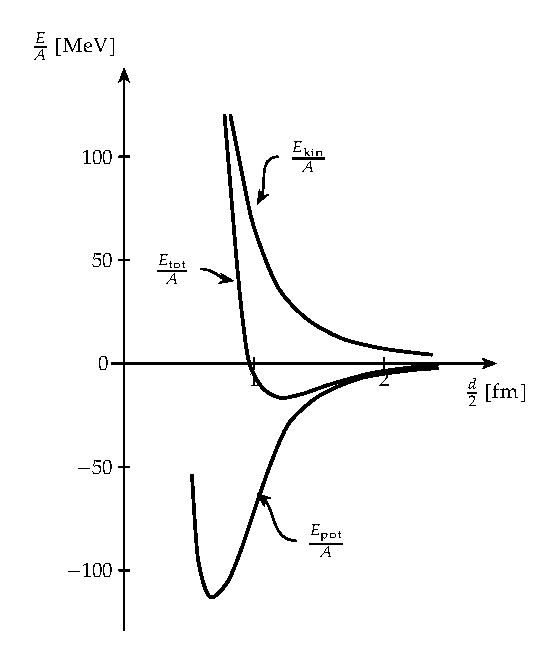
\includegraphics[width=0.45\linewidth]{pictures/1_1}
\par\end{centering}
\centering{}\caption{\label{fig:1_1}核饱和作为动能与势能微小差异效应的定性解释。}
\end{figure}

核力的饱和性质也定性的解释了实验上发现的一些现象（通过电子散射，$\mu$子x-射线等实验发现的），例如原子核内部相对平均的密度和原子核相对确定的表面。现在我们可以用一个具有常数密度和确定表面
\begin{comment}
与模糊的表面相对，实际上就是在说密度分布有一个突变。
\end{comment}
的球来描述原子核了，于是半径为：
\[
R=r_{0}A^{1/3}
\]

经验上讲，参数$r_{0}$的值为：
\[
r_{0}=1.2\,\text{fm}
\]

在\ref{fig:1_2}中，我们可以看出比结合能对于质量数$A$依赖的细节。

\begin{figure}[H]
\begin{centering}
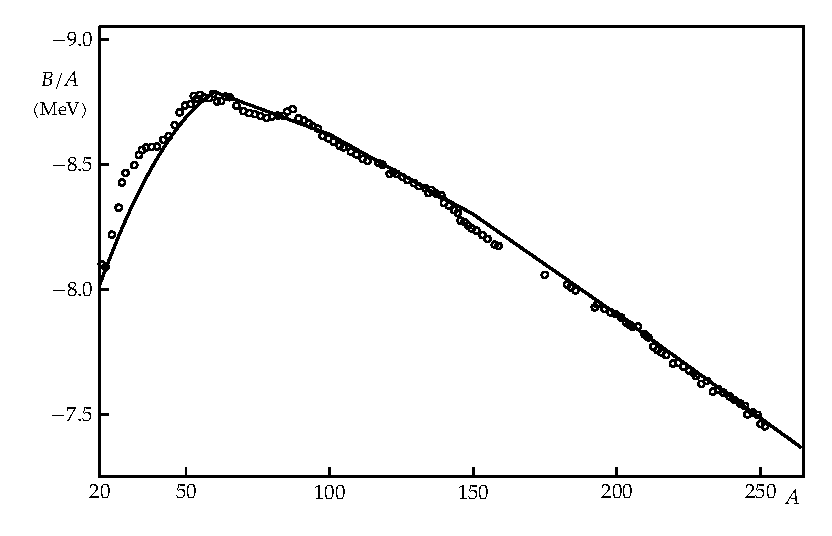
\includegraphics[width=0.68\linewidth]{pictures/1_2}
\par\end{centering}
\centering{}\caption{\label{fig:1_2}实验测得的$\beta$稳定奇$A$核的比结合能和利用类似质量公式计算出的曲线}
\end{figure}

$A=12$以前，比结合能迅速增加直到$B/A\simeq8\,\text{MeV}$，在$A\simeq60$时，比结合能达到最大，稍低于$9\,\text{MeV}$。在此之后，比结合能缓慢下降，直到$A=250$的时候，比结合能降为了大约$7.5\,\text{MeV}$。这是质子的库伦排斥的影响越来越大导致的。

曾经有过很多尝试试图得到$B/A$与$N$、$Z$的函数关系。最著名的公式是Bethe和Weizsci\"acker{[}We
35, BB 36{]}得到的半经验质量公式：
\begin{equation}
B(N,Z)=a_{V}A+a_{S}A^{2/3}+a_{C}\frac{Z^{2}}{A^{1/3}}+a_{I}\frac{(N-Z)^{2}}{A}-\delta(A)\label{eq:semiempirical mass formula}
\end{equation}

拟合得到的合适的参数为{[}MS 66, My 69, MS 69{]}：
\begin{gather*}
a_{V}=-15.68;\quad a_{S}=18.56;\quad a_{C}=0.717;\quad a_{I}=28.1\,\text{MeV}\\
\delta(A)=\begin{cases}
34\cdot A^{-3/4} & \text{偶偶核}\\
0 & \text{奇偶核}\\
-34\cdot A^{-3/4} & \text{奇奇核}
\end{cases}
\end{gather*}

在\ref{fig:1_2}中我们看到，利用这个半经验公式我们得到了非常好的基本符合实验结果的曲线。

接下来我们阐释公式\ref{eq:semiempirical mass formula}的物理意义。第一项通常被称为体积项，因为它正比于$A$，即正比于$R^{3}$。$a_{V}$之所以不等于比结合能$-8.5\,\text{MeV}$，是因为在求比结合能时，需要对很多核做平均，而其它项如$a_{S},a_{C},a_{I}$作平均后是个正的常数。

第二项正比于$A^{2/3}$即$R^{2}$，因此它被称为表面项。它是表面的核子对总结合能的贡献比较小导致的。我们可以从$a_{S}$中得出表面张力系数（定义为单位表面积贡献的能量）：
\[
\sigma=\frac{a_{S}}{4\mathrm{\pi}r^{2}_{0}}=1.03\,\text{MeV\ensuremath{\cdot}\text{fm}}^{-2}
\]

第三项考虑了库伦相互作用。如果我们近似的把原子核看成是电荷均匀分布的球体，那么它就可以计算出来。原子核体系的库仑能正比于质子数的平方，反比于半径。

因为质子会互相排斥，似乎原子核会倾向于有更多的中子，但这是并未考虑泡利不相容原理的结果。事实上，如果一个质子发生$\beta$衰变变成中子，这个中子会成为中子费米面之上的态（见第二章），这从能量的角度上讲是不容易发生的。第四项即考虑了这一平衡，根据费米气体模型，它正比于$(N-Z)^{2}/A$，它会促使质子数和中子数相同，被称为对称能。这一结合能和$N-Z$的二次方关系和实验也符合的非常好。

考虑了这四项之后，和实验结果唯一的不同就是考虑偶偶核，奇偶核和奇奇核时的区别。在第六章我们会看到，这是所谓的对效应导致的。我们在第五项中考虑了这一点。

第十三章我们讨论Thomas-Fermi方法时会再次讨论半经验质量公式。

需要指出的是，半经验质量公式只是整体上很好的拟合了结合能关于$A$的函数，局部上仍会出现较大的偏离。这主要是壳效应导致的，我们在2.9部分会讨论这一点。

\section{形变参数}

到目前为止，我们只研究了液滴模型的静态性质。接下来我们会假设原子核具有一个确定的表面，但却不一定是球面。并且我们会想象它发生动力学形变和表面的振动。

在我们研究这些振动之前，我们必须用一些参数来描述表面。一个可能的方式是用原子核中心到表面的径矢长度来描述：
\begin{equation}
R=R(\theta,\phi)=R_{0}\left(1+\alpha_{00}+\sum^{\infty}_{\lambda=1}\sum^{\lambda}_{\mu=-\lambda}\alpha^{*}_{\lambda\mu}Y_{\lambda\mu}(\theta,\phi)\right)\label{eq:expansion of R}
\end{equation}

这里$R_{0}$是具有相同体积的球面的半径
\begin{comment}
这里的所有$\alpha$都是小参数。
\end{comment}
。这样的表面不是最一般的形式\footnote{例如裂变中裂成两半的核。}，但却是在核结构中非常有用的形式。

参数$\alpha_{00}$描述了核的体积变化。我们知道原子核的不可压缩性非常之强，因此在发生任何形变时，核的体积应当保持不变：
\[
V=\frac{4}{3}\mathrm{\pi}R^{3}_{0}
\]

这定义了参数$\alpha_{00}$，至多到二阶，我们得到\cite{EG70}：
\[
\alpha_{00}=-\frac{1}{4\mathrm{\pi}}\sum_{\lambda\geq1,\mu}\left|\alpha_{\lambda\mu}\right|^{2}
\]

\begin{booknote*}
使用$R(\theta,\phi)$计算核的体积，应当有：
\begin{align*}
V & =\int^{R}_{0}r^{2}\sin\theta\mathrm{d}r\mathrm{d}\theta\mathrm{d}\phi=\frac{1}{3}\int R^{3}\sin\theta\mathrm{d}\theta\mathrm{d}\phi\\
 & =\frac{1}{3}R^{3}_{0}\int\left(1+\alpha_{00}+\sum^{\infty}_{\lambda=1}\sum^{\lambda}_{\mu=-\lambda}\alpha^{*}_{\lambda\mu}Y_{\lambda\mu}(\theta,\phi)\right)^{3}\sin\theta\mathrm{d}\theta\mathrm{d}\phi
\end{align*}

保留到$\alpha$的二阶项，得到：
\begin{align*}
V & =\frac{1}{3}R^{3}_{0}\int1+3\alpha_{00}+3\alpha^{2}_{00}+3(1+2\alpha_{0})\left(\sum^{\infty}_{\lambda=1}\sum^{\lambda}_{\mu=-\lambda}\alpha^{*}_{\lambda\mu}Y_{\lambda\mu}(\theta,\phi)\right)\\
 & +3\left(\sum^{\infty}_{\lambda=1}\sum^{\lambda}_{\mu=-\lambda}\alpha^{*}_{\lambda\mu}Y_{\lambda\mu}(\theta,\phi)\right)^{2}\sin\theta\mathrm{d}\theta\mathrm{d}\phi
\end{align*}

球谐函数的一次项积分应当为零，二次项可以如下得到：由于$R$为实数，因此$R^{2}$可以写为$R^{*}R$，由此可以利用球谐函数的正交性得到结果：
\[
V=\frac{4}{3}\mathrm{\pi}R^{3}_{0}+4\mathrm{\pi}\alpha_{00}(1+\alpha_{00})R^{3}_{0}+\sum_{\lambda\geq1,\mu}\left|\alpha_{\lambda\mu}\right|^{2}R^{3}_{0}
\]

由此我们得到：
\[
4\mathrm{\pi}\alpha_{00}(1+\alpha_{00})R^{3}_{0}+\sum_{\lambda\geq1,\mu}\left|\alpha_{\lambda\mu}\right|^{2}R^{3}_{0}=0
\]
我们考虑如下方程：
\[
x(1+x)+a=0
\]

其中$x$，$a$均是小量，我们可以解得：
\begin{align*}
x=\frac{-1\pm\sqrt{1-4a}}{2}
\end{align*}

保留到一阶，得：
\[
x=-\frac{1}{2}\pm\frac{1}{2}(1-2a)=-a/(a-1)
\]

由于$x$是小量，因此$x=-a$。

回归到上述问题，我们得到：
\[
\alpha_{00}=-\frac{1}{4\mathrm{\pi}}\sum_{\lambda\geq1,\mu}\left|\alpha_{\lambda\mu}\right|^{2}
\]
\end{booknote*}
$\lambda=1$的项主要描述了整个体系的平移（至少对于小形变来说）。当原点取在质心处时，$\alpha_{1\mu}$这三个参数可以唯一确定。此时有：
\[
\int_{V}\boldsymbol{r}\,\mathrm{d}^{3}\boldsymbol{r}=0
\]

\begin{booknote*}
考虑质心发生了移动，$(x,y,z)$变成了$(x+x_{0},y+y_{0},z+z_{0})$，其中$x_{0},y_{0},z_{0}$均为小量。把直角坐标转换成球坐标，保留到一阶得到：
\[
R^{\prime}=\sqrt{(x+x_{0})^{2}+(y+y_{0})^{2}+(z+z_{0})^{2}}\approx R+\frac{xx_{0}+yy_{0}+zz_{0}}{x^{2}+y^{2}+z^{2}}
\]

因此把$R^{\prime}$用$\theta^{\prime},\phi^{\prime}$表示出来，必定有：
\[
R^{\prime}=R+\sin\theta^{\prime}\cos\phi^{\prime}x_{0}+\sin\theta^{\prime}\sin\phi^{\prime}y_{0}+\cos\theta^{\prime}z_{0}
\]

根据球谐函数的表达式，一阶项可以写成$Y_{1,-1}$，$Y_{1,0}$，$Y_{1,1}$的线性和。

我们由此证明了$\lambda=1$的项描述了整个体系的平移。
\end{booknote*}
如果展开式\ref{eq:expansion of R}仅包含$\lambda$的偶数值，则该条件自动满足
\begin{comment}
我不知道他为什么要强调这一点。
\end{comment}
。在其他情形下，$\alpha_{1\mu}$则从$\alpha_{\lambda\mu}\,(\lambda>2)$的二阶项开始
\begin{comment}
我看不懂它在说什么。
\end{comment}
。因此，由于我们在后续讨论中将限制于小形变情形，我们将同时略去$\alpha_{00}$与$\alpha_{1\mu}$
\begin{comment}
为什么可以忽略$\alpha_{00}$？我认为是不能省的，因此后面的推导没有省略，并且得到了正确的结果。
\end{comment}
。

看一看展开式\ref{eq:expansion of R}中最低阶的多级形变是有益的，如\ref{fig:1_3}。$\lambda=2$的对应的形变看起来像椭球形变。然而，需要注意的是这仅仅精确到了小参数的一阶。一个真正的椭球的表达式中，$\lambda>2$的项也都是存在的。

\begin{figure}[H]
\begin{centering}
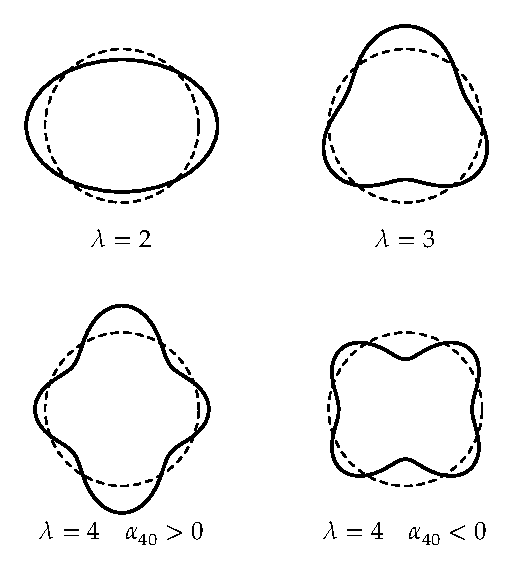
\includegraphics[width=0.48\linewidth]{pictures/1_3}
\par\end{centering}
\centering{}\caption{\label{fig:1_3}多级形变}
\end{figure}

此外，径矢长度$R$在反演变换和转动变换下应当是不变的
\begin{comment}
形式应当是不变的，变化的只是参数的值。根据球谐函数的完备性，我觉得这并不构成所谓的“限制”，只是我们推导出了坐标系在相应变换下新参数和旧参数的关系。
\end{comment}
，这对$\alpha_{\lambda\mu}$构成了限制。为此，$\alpha_{\lambda\mu}$在反演变换下必须乘上$(-)^{\lambda}$，并且在转动变换下必须像一个球谐函数一样变换。即如果转动了Euler角$\Omega=(\alpha,\beta,\gamma)$的话，应当有：
\begin{align*}
(Y_{\lambda\mu})_{\text{new}} & =\sum_{\mu^{\prime}}D^{\lambda}_{\mu^{\prime}\mu}(\Omega)(Y_{\lambda\mu^{\prime}})_{\text{old}}\\
a_{\lambda\mu} & =\sum_{\mu^{\prime}}D^{\lambda}_{\mu^{\prime}\mu}(\Omega)\alpha_{\lambda\mu^{\prime}}
\end{align*}

这里$D^{\lambda}_{\mu^{\prime}\mu}(\Omega)$是转动的Wigner函数，$a_{\lambda\mu}$是转动后参考系中的形变参数。
\begin{booknote*}
变换参考系后的径矢长度$R^{\prime}$用新参考系中的坐标$\theta^{\prime}$，$\phi^{\prime}$表示为：
\[
R^{\prime}(\theta^{\prime},\phi^{\prime})=R_{0}\left(1+\alpha_{00}+\sum^{\infty}_{\lambda=2}\sum_{\mu}a^{*}_{\lambda\mu}Y_{\lambda\mu}(\theta^{\prime},\phi^{\prime})\right)
\]

利用：
\[
Y_{\lambda\mu}(\theta^{\prime},\phi^{\prime})=\sum_{\mu^{\prime}}D^{\lambda}_{\mu^{\prime}\mu}(\Omega)Y_{\lambda\mu^{\prime}}(\theta,\phi)
\]

得到：
\[
R^{\prime}(\theta^{\prime},\phi^{\prime})=R_{0}\left(1+\alpha_{00}+\sum^{\infty}_{\lambda=2}\sum_{\mu\mu^{\prime}}a^{*}_{\lambda\mu}D^{\lambda}_{\mu^{\prime}\mu}(\Omega)Y_{\lambda\mu^{\prime}}(\theta,\phi)\right)
\]

因此要求：
\[
\sum_{\mu}a^{*}_{\lambda\mu}D^{\lambda}_{\mu^{\prime}\mu}(\Omega)=\alpha^{*}_{\lambda\mu^{\prime}}
\]

利用$D^{\lambda}_{\mu^{\prime}\mu}(\Omega)=D^{\lambda*}_{\mu\mu^{\prime}}(\Omega^{-1})$，得到：
\[
\sum_{\mu}a_{\lambda\mu}D^{\lambda}_{\mu\mu^{\prime}}(\Omega^{-1})=\alpha_{\lambda\mu^{\prime}}
\]

此即：
\[
a_{\lambda\mu}=\sum_{\mu^{\prime}}D^{\lambda}_{\mu^{\prime}\mu}(\Omega)\alpha_{\lambda\mu^{\prime}}
\]

由此得到：
\[
R^{\prime}(\theta^{\prime},\phi^{\prime})=R_{0}\left(1+\alpha_{00}+\sum^{\infty}_{\lambda=2}\sum_{\mu^{\prime}}\alpha^{*}_{\lambda\mu^{\prime}}Y_{\lambda\mu^{\prime}}(\theta,\phi)\right)=R(\theta,\phi)
\]

由推导中也看出了一开始引入的$\alpha^{*}$中star的作用。
\end{booknote*}
为了确保\ref{eq:expansion of R}中的径矢长度$R$是实的，我们必须利用性质$Y^{*}_{\lambda\mu}=(-)^{\mu}Y_{\lambda,-\mu}$得到：
\[
\alpha^{*}_{\lambda\mu}=(-)^{\mu}\alpha_{\lambda,-\mu}
\]

之后可以证明，这恰恰是$\alpha_{\lambda\mu}$在时间反演下的行为。
\begin{booknote*}
利用上述性质，应当有：
\begin{align*}
\alpha^{*}_{\lambda\mu}Y_{\lambda\mu}+\alpha^{*}_{\lambda,-\mu}Y_{\lambda,-\mu} & =\alpha^{*}_{\lambda\mu}Y_{\lambda\mu}+\alpha^{*}_{\lambda,-\mu}(-)^{\mu}Y^{*}_{\lambda\mu}
\end{align*}

为了使它们组合出常数，两项应当互为共轭，得到：
\[
\alpha^{*}_{\lambda\mu}=(-)^{\mu}\alpha_{\lambda,-\mu}
\]
\end{booknote*}
在讨论普适的表面多级振动之前，我们需要提及两种特殊的情况：
\begin{enumerate}
\item 第一种是轴对称的形变。如果选取$z$轴为对称轴，我们会发现$\alpha_{\lambda\mu}$只有$\mu=0$的情况下才不为零。$\alpha_{\lambda0}$通常称作$\beta_{\lambda}$。
\item 在偶极形变（$\lambda=2$）的情况下，我们有五个$\alpha_{\lambda\mu}$参数。它们并没有都描述了液滴的形状。事实上，其中有三个描述了液滴的取向，和三个Euler角有关。通过一个合适的转动，我们可以把参考系转动到三个轴1，2，3表征的体坐标系，这三个轴和液滴的质量分布的主轴是对应的。转动之后，五个参数$\alpha_{2\mu}$变为了两个独立变量$a_{20}$和$a_{22}=a_{2,-2}$（$a_{21}=a_{2,-1}=0$），这两个变量和三个Euler角一起，完整的描述了这个系统。为了方便，我们引入Hill-Wheeler坐标$\beta,\gamma$，他们和$a_{20}$，$a_{22}$的关系为：
\begin{align*}
a_{20} & =\beta\cdot\cos\gamma\\
a_{22} & =\frac{1}{\sqrt{2}}\cdot\beta\cdot\sin\gamma
\end{align*}

由此我们得到：
\[
\sum_{\mu}\left|\alpha_{2\mu}\right|^{2}=a^{2}_{20}+2a^{2}_{22}=\beta^{2}
\]

以及：
\[
R(\theta,\phi)=R_{0}\left\{ 1+\beta\sqrt{\frac{5}{16\mathrm{\pi}}}[\cos\gamma(3\cos^{2}\theta-1)+\sqrt{3}\sin\gamma\sin^{2}\theta\cos2\phi]\right\} 
\]

\end{enumerate}
在\ref{fig:1_4}中，我们在极坐标$\beta$，$\gamma$中表示了偶极形变的形状。我们可以看出：
\begin{enumerate}
\item $\gamma$的值为$0^{\circ}$，$120^{\circ}$，$240^{\circ}$时，为以3，1，2轴为对称轴的长椭球。
\item $\gamma$的值为$180^{\circ}$，$300^{\circ}$，$60^{\circ}$时为对应的扁椭球。
\item 其他情形对应三轴形变（triaxial shapes）
\begin{comment}
按照我画的图看，意思应该是不是柱对称的。
\end{comment}
。
\item 存在离散对称性，也就是说，我们可以随意交换三个轴而不改变形状。这意味着点群$D_{2}$下的不变性
\begin{comment}
提这个有意义吗？——看到点群就烦的译者。
\end{comment}
。因此，$0<\gamma<60^{\circ}$可以描述所有偶极形变，其它形状可以通过交换轴得到。
\end{enumerate}
\begin{figure}[H]
\begin{centering}
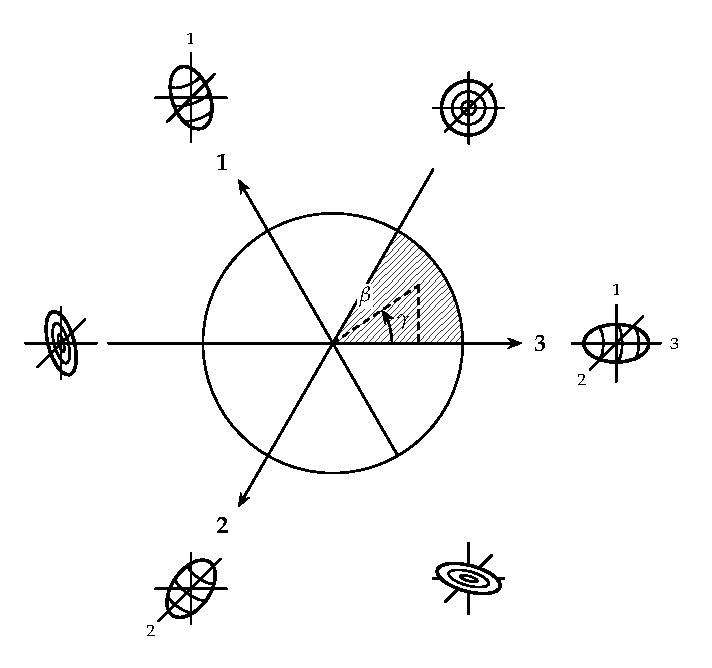
\includegraphics[width=0.52\linewidth]{pictures/1_4}
\par\end{centering}
\centering{}\caption{\label{fig:1_4}Hill-Wheeler坐标下的原子核形状}
\end{figure}

\begin{enumerate}
\item 可以计算出$\beta$和$\gamma$引起的椭球半轴变化量：
\begin{align*}
\delta R_{1} & =R(\frac{\mathrm{\pi}}{2},0)-R_{0}=R_{0}\sqrt{\frac{5}{4\mathrm{\pi}}}\beta\cos\left(\gamma-\frac{2\mathrm{\pi}}{3}\right)\\
\delta R_{2} & =R(\frac{\mathrm{\pi}}{2},\frac{\mathrm{\pi}}{2})-R_{0}=R_{0}\sqrt{\frac{5}{4\mathrm{\pi}}}\beta\cos\left(\gamma+\frac{2\mathrm{\pi}}{3}\right)\\
\delta R_{3} & =R(0,0)-R_{0}=R_{0}\sqrt{\frac{5}{4\mathrm{\pi}}}\beta\cos\gamma
\end{align*}

即：
\[
\delta R_{\kappa}=R_{0}\sqrt{\frac{5}{4\mathrm{\pi}}}\beta\cos\left(\gamma-\frac{2\mathrm{\pi}}{3}\kappa\right),\quad\kappa=1,2,3
\]

我们必须强调，$\beta$和$\gamma$仅在小参数的情况下描述了椭球形变。
\end{enumerate}

\section{球形的表面振动}

第一种类型的激发是动力学的形状或表面振动。此时的动力学变量是描述表面的参数，例如\ref{eq:expansion of R}中的$\alpha_{\lambda\mu}(\lambda\geq2)$。它们被认为是时间的函数：$\alpha_{\lambda\mu}(t)$。我们可以期待，低能激发实际上是$\alpha_{\lambda\mu}=0$（对应球面）附近的一些小振动，描述这一过程的Hamilton量具有谐振子的形式：
\begin{equation}
H_{\text{coll}}=T+V=\frac{1}{2}\sum_{\lambda\mu}\left(B_{\lambda}\left|\dot{\alpha}_{\lambda\mu}\right|^{2}+C_{\lambda}\left|\alpha_{\lambda\mu}\right|^{2}\right)\label{eq:Hamiltonian of vibrating sphere}
\end{equation}

这里惯性系数$B_{\lambda}$和刚度系数$C_{\lambda}$是实参数。这实际上是由转动不变和时间反演不变\footnote{关于时间反演，Messiah\cite{Me61}中有更多细节。在无自旋系统中，同这里一样，时间反演与复共轭相联系。}所确定的唯一可能的二次形式。

利用正则量子化，我们得到量子化后的形式：
\[
\hat{H}_{\text{coll}}=\sum_{\lambda\mu}\hbar\Omega_{\lambda}\left(B^{\dagger}_{\lambda\mu}B_{\lambda\mu}+\frac{1}{2}\right)
\]

这里频率为：
\[
\Omega_{\lambda}=\left(\frac{C_{\lambda}}{B_{\lambda}}\right)^{\frac{1}{2}}
\]

算符$B_{\lambda\mu}$满足Bose对易关系：
\[
[B_{\lambda\mu},B_{\lambda^{\prime}\mu^{\prime}}]=0;\quad[B_{\lambda\mu},B^{\dagger}_{\lambda^{\prime}\mu^{\prime}}]=\delta_{\lambda\lambda^{\prime}}\delta_{\mu\mu^{\prime}}
\]

并且存在一个Bose真空$|0\rangle$使得$B_{\lambda\mu}|0\rangle=0$。Bose算符$B_{\lambda\mu}$和坐标算符$\hat{\alpha}_{\lambda\mu}$和相应的动量算符$\hat{\pi}_{\lambda\mu}$的关系如下：
\begin{align*}
\hat{\alpha}_{\lambda\mu} & =\left(\frac{\hbar}{2B_{\lambda}\Omega_{\lambda}}\right)^{\frac{1}{2}}[B^{\dagger}_{\lambda\mu}+(-)^{\mu}B_{\lambda,-\mu}]\\
\hat{\pi}_{\lambda\mu} & =\mathrm{i}\left(\frac{\hbar}{2}B_{\lambda}\Omega_{\lambda}\right)^{\frac{1}{2}}[(-)^{\mu}B^{\dagger}_{\lambda,-\mu}-B_{\lambda\mu}]
\end{align*}

\begin{booknote*}
根据Hamilton量写出动量：
\begin{align*}
\pi_{\lambda\mu} & =\frac{\partial H_{\text{coll}}}{\partial\dot{\alpha}_{\lambda\mu}}=\frac{1}{2}\sum_{\lambda^{\prime}\mu^{\prime}}B_{\lambda^{\prime}}\frac{\partial}{\partial\dot{\alpha}_{\lambda\mu}}\dot{\alpha}^{*}_{\lambda^{\prime}\mu^{\prime}}\dot{\alpha}_{\lambda^{\prime}\mu^{\prime}}\\
 & =\frac{1}{2}\sum_{\lambda^{\prime}\mu^{\prime}}B_{\lambda^{\prime}}\frac{\partial}{\partial\dot{\alpha}_{\lambda\mu}}(-)^{\mu^{\prime}}\dot{\alpha}_{\lambda^{\prime},-\mu^{\prime}}\dot{\alpha}_{\lambda^{\prime}\mu^{\prime}}\\
 & =B_{\lambda}\dot{\alpha}^{*}_{\lambda\mu}
\end{align*}

于是Hamilton量变为：
\[
H_{\text{coll}}=\frac{1}{2}\sum_{\lambda\mu}\left(\frac{1}{B_{\lambda}}\left|\pi_{\lambda\mu}\right|^{2}+C_{\lambda}\left|\alpha_{\lambda\mu}\right|^{2}\right)
\]

根据正则量子化步骤，引入Bose对易关系：
\[
[\hat{\alpha}_{\lambda\mu},\hat{\pi}_{\lambda^{\prime}\mu^{\prime}}]=\mathrm{i}\hbar\delta_{\lambda\lambda^{\prime}}\delta_{\mu\mu^{\prime}}
\]

并按照前面的定义引入$B_{\lambda\mu}$和$B^{\dagger}_{\lambda\mu}$，经验证可以满足产生湮灭算符的对应关系。与此同时，Hamilton量变为期望的谐振子形式。
\end{booknote*}
从上面的讨论中，我们得到对每一个$\lambda$，都有一个相应的表面振动谐振子谱与之对应，正如\ref{fig:1_5}。

\begin{figure}[H]
\begin{centering}
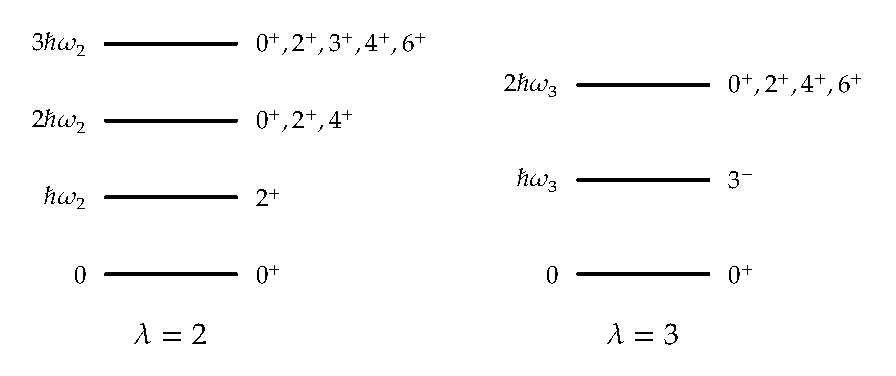
\includegraphics[width=0.55\linewidth]{pictures/1_5}
\par\end{centering}
\centering{}\caption{\label{fig:1_5}四极（$\lambda=2$）和八极（$\lambda=3$）表面振动的简谐能谱}
\end{figure}

根据$\alpha_{\lambda\mu}$和$B^{\dagger}_{\lambda\mu}$在坐标系转动下都如同球张量一样变换，我们可以得到$B^{\dagger}_{\lambda\mu}$与角动量算符的对易关系，并发现单玻色子态$|\lambda\mu\rangle=B^{\dagger}_{\lambda\mu}|0\rangle$有角动量$I=\lambda$，$z$-分量$M=\mu$，宇称$(-)^{\lambda}$。
\begin{booknote*}
坐标变换下：
\[
\hat{a}_{\lambda\mu}=\sum_{\mu^{\prime}}D^{\lambda}_{\mu^{\prime}\mu}(\Omega)\hat{\alpha}_{\lambda\mu^{\prime}}
\]

由此$\hat{\pi}_{\lambda\mu}$在坐标变换下：
\begin{align*}
\hat{p}_{\lambda\mu} & =B_{\lambda}\dot{\hat{\alpha}}^{*}_{\lambda\mu}=B_{\lambda}\sum_{\mu^{\prime}}D^{\lambda*}_{\mu^{\prime}\mu}(\Omega)\dot{\hat{\alpha}}^{*}_{\lambda\mu^{\prime}}\\
 & =\sum_{\mu^{\prime}}D^{\lambda*}_{\mu^{\prime}\mu}(\Omega)\hat{\pi}_{\lambda\mu^{\prime}}
\end{align*}

可知$\hat{p}^{\dagger}_{\lambda\mu}=\sum_{\mu^{\prime}}D^{\lambda}_{\mu^{\prime}\mu}(\Omega)\hat{\mathrm{\pi}}_{\lambda\mu^{\prime}}$，与$\hat{\alpha}_{\lambda\mu}$的变换相同。再根据：
\[
B^{\dagger}_{\lambda\mu}=\frac{1}{2}\left[\left(\frac{2}{\hbar}B_{\lambda}\Omega_{\lambda}\right)^{\frac{1}{2}}\hat{\alpha}_{\lambda\mu}+\mathrm{i}\left(\frac{2}{\hbar B_{\lambda}\Omega_{\lambda}}\right)^{\frac{1}{2}}\hat{\mathrm{\pi}}^{\dagger}_{\lambda\mu}\right]
\]

可知$B^{\dagger}_{\lambda\mu}$同$\alpha_{\lambda\mu}$变换也相同。之后的结论参考角动量与球张量。
\end{booknote*}
为了构建多玻色子态，我们必须利用角动量耦合的规则，并且考虑置换对称性
\begin{comment}
为何要考虑？
\end{comment}
。例如，考虑两个四极玻色子（$\lambda=2$）的叠加，三种可能的组合为$I^{\pi}=0^{+},2^{+},4^{+}$。
\[
|IM\rangle=\frac{1}{\sqrt{2}}\sum_{\mu_{1}\mu_{2}}C^{22I}_{\mu_{1}\mu_{2}M}B^{\dagger}_{2\mu_{1}}B^{\dagger}_{2\mu_{2}}|0\rangle
\]

$I=1,3$的态都会消失，因为Clebsch-Gordon系数\footnote{这里我们利用$C^{j_{1}j_{2}j_{3}}_{m_{1}m_{2}m_{3}}$来表示$\langle j_{1}m_{1}j_{2}m_{2}|j_{1}j_{2}j_{3}m_{2}\rangle$。}的在$\mu_{1}$和$\mu_{2}$交换时的性质：
\[
C^{22I}_{\mu_{1}\mu_{2}M}=(-)^{I}C^{22I}_{\mu_{2}\mu_{1}M}
\]

事实上，许多球形核的谱中有一个低能的$2^{+}$态。大约在两倍的激发能
\begin{comment}
第一激发态的能量。
\end{comment}
处，还有所谓的两玻色子三重态（$0^{+}$，$2^{+}$，$4^{+}$），然而，这三个态的能谱通常分开一点点。

常数$B_{\lambda}$和$C_{\lambda}$可以在流体图像中计算出来；它们取决于与表面振动相关的流动。因此，有必要假设液滴内流体运动的性质。
\begin{comment}
此时，我们需要再次讨论核液体这一概念的含义。在第十三章，我们将会仔细研究这一点并且发现核实际上是费米液体而不是普通的液体，这一点非常重要。（我觉得这是不需要说的话，但是是书上有的，我把它放在了脚注里。
\end{comment}
我们可以做的最简单的假设是流体是无旋的，即$\nabla\times\boldsymbol{v}(\boldsymbol{r})=0$，这里$\boldsymbol{v}$是速度场。我们在第十三章中还会研究这一假定，但是现在先让我们接受它：
\[
\boldsymbol{v}(t)=-\nabla\Phi(\boldsymbol{r})
\]

下一个假设是不可压缩性，这对于原子核来说是十分合理的。这意味着原子核密度是个常数（$\dot{\rho}=0$），根据连续性方程，我们可以得到：
\[
\nabla\cdot\boldsymbol{v}=0
\]

由此，得到：
\[
\nabla^{2}\Phi=0
\]

上述方程在原点处不发散的最一般的解是：
\[
\Phi(\boldsymbol{r})=\sum_{\lambda\mu}d^{*}_{\lambda\mu}r^{\lambda}Y_{\lambda\mu}(\theta,\phi)
\]

对于小形变，精确到一阶，边界条件可以为：
\[
v_{r}=-\frac{\partial}{\partial r}\Phi=\dot{R}\quad\text{at}\quad r=R_{0}
\]

由此，代入\ref{eq:expansion of R}即可得到系数$d_{\lambda\mu}$和$\alpha_{\lambda\mu}$的关系：
\[
d_{\lambda\mu}=-\frac{1}{\lambda}R^{2-\lambda}_{0}\dot{\alpha}_{\lambda\mu}
\]

\begin{booknote*}
边界条件为：
\[
-\sum_{\lambda\mu}d^{*}_{\lambda\mu}\lambda R^{\lambda-1}_{0}Y_{\lambda\mu}(\theta,\phi)=R_{0}\left(\sum_{\lambda\mu}\dot{\alpha}^{*}_{\lambda\mu}Y_{\lambda\mu}(\theta,\phi)\right)
\]

根据球谐函数正交性可得：
\[
d^{*}_{\lambda\mu}=-\frac{1}{\lambda}R^{2-\lambda}_{0}\dot{\alpha}^{*}_{\lambda\mu}
\]
\end{booknote*}
表面振动的动能为：
\[
T=\frac{m}{2}\rho\int_{V}v^{2}(\boldsymbol{r})\,\mathrm{d}^{3}\boldsymbol{r}=\frac{m}{2}\rho\int_{V}\left|\nabla\Phi\right|^{2}\,\mathrm{d}^{3}\boldsymbol{r}=\frac{m}{2}\rho\oint_{S}\Phi^{*}\nabla\Phi\cdot\mathrm{d}\boldsymbol{S}
\]

这里$\rho$是质量为$m$的核子密度，是一个常数。利用球谐函数的梯度公式
\begin{comment}
狗屁，哪里用到了。
\end{comment}
，我们得到小形变近似下的动能为：
\begin{equation}
T=\frac{R^{5}_{0}m\rho}{2}\sum_{\lambda\mu}\frac{\left|\dot{\alpha}_{\lambda\mu}\right|^{2}}{\lambda}\label{eq:kinetic energy of little alpha}
\end{equation}

\begin{booknote*}
利由于梯度要与$\mathrm{d}\boldsymbol{S}$相乘，因此只需要计算$r$分量，用球坐标梯度公式得：
\begin{align*}
\nabla r^{\lambda}Y_{\lambda\mu}(\theta,\phi) & =\lambda r^{\lambda-1}Y_{\lambda\mu}(\theta,\phi)\hat{\boldsymbol{e}}_{r}
\end{align*}

由此推得动能为：
\begin{align*}
T & =\frac{m\rho}{2}\oint_{S}\sum_{\lambda\mu}d_{\lambda\mu}r^{\lambda}Y^{*}_{\lambda\mu}(\theta,\phi)\nabla\left(\sum_{\lambda^{\prime}\mu^{\prime}}d^{*}_{\lambda^{\prime}\mu^{\prime}}r^{\lambda^{\prime}}Y_{\lambda^{\prime}\mu^{\prime}}(\theta,\phi)\right)\cdot\mathrm{d}\boldsymbol{S}\\
 & =\frac{m\rho}{2}\sum_{\lambda\mu}\sum_{\lambda^{\prime}\mu^{\prime}}d_{\lambda\mu}d^{*}_{\lambda^{\prime}\mu^{\prime}}\lambda^{\prime}R^{\lambda+\lambda^{\prime}-1}_{0}\oint_{S}Y^{*}_{\lambda\mu}(\theta,\phi)Y_{\lambda^{\prime}\mu^{\prime}}(\theta,\phi)\,\mathrm{d}S\\
 & =\frac{m\rho}{2}\sum_{\lambda\mu}\left|d_{\lambda\mu}\right|^{2}\lambda R^{2\lambda+1}_{0}\\
 & =\frac{R^{5}_{0}m\rho}{2}\sum_{\lambda\mu}\frac{\left|\dot{\alpha}_{\lambda\mu}\right|^{2}}{\lambda}
\end{align*}
\end{booknote*}
与\ref{eq:Hamiltonian of vibrating sphere}对比，得：
\[
B_{\lambda}=\frac{\rho mR^{5}_{0}}{\lambda}=\frac{3}{4\mathrm{\pi}\lambda}A\cdot mR^{2}_{0}
\]

对于球形表面的振动而言，质量参数并不是$\mu$的函数，然而对于形变的液滴而言，这并不正确。

如果我们忽略对称能和对能的改变的话，$\alpha_{\lambda\mu}$所表征的液滴的表面形变的势能可以从Bethe-Weizs\"acker公式\ref{eq:semiempirical mass formula}的系数中得到。

由于我们假设了不可压缩性，因此体积项是与形变无关的。然而这只对普通液体正确，事实上，在第十三章中我们可以看到，对量子液体而言体积项会有一个微小的改变。当然在通常的处理中，体积项并不需要考虑，因此形变能只有两项，分别是表面能和库仑能。在第十三章我们会讨论更多细节，并得到这仅仅对于单极和偶极形变是足够的。

形变能被定义为形变液滴和球形液滴的能量差：
\[
V(\alpha)=E_{S}(\alpha)-E_{S}(0)+E_{C}(\alpha)-E_{C}(0)
\]

表面能可以由表面积和表面张力系数$\sigma$相乘得到。类似\ref{eq:kinetic energy of little alpha}的推导
\begin{comment}
相似你个大头鬼。
\end{comment}
，我们可以得到至多到$\alpha_{\lambda\mu}$二阶的表面能：
\[
E_{S}(\alpha)=\sigma\oint_{S}\mathrm{d}S=E_{S}(0)+\frac{1}{2}\sum_{\lambda\mu}(\lambda-1)(\lambda+2)R^{2}_{0}\sigma\left|\alpha_{\lambda\mu}\right|^{2}
\]

\begin{booknote*}
利用梯度求出垂直于$R(\theta,\phi)$的矢量：
\begin{align*}
\nabla R(\theta,\phi) & =\frac{1}{r}\frac{\partial}{\partial\theta}R(\theta,\phi)\hat{\boldsymbol{e}}_{\theta}+\frac{1}{r\sin\theta}\frac{\partial}{\partial\phi}R(\theta,\phi)\hat{\boldsymbol{e}}_{\phi}\\
\nabla(r-R(\theta,\phi)) & =\hat{\boldsymbol{e}}_{r}-\nabla R(\theta,\phi)
\end{align*}

这个矢量的模为：
\[
\left|\hat{\boldsymbol{e}}_{r}-\nabla R\right|=\sqrt{1+(\nabla R)^{2}}
\]

$R(\theta,\phi)$面元与球面元的夹角等于该矢量和$\hat{\boldsymbol{e}}_{r}$的夹角：
\[
\cos\alpha=\frac{(\hat{\boldsymbol{e}}_{r}-\nabla R)\cdot\hat{\boldsymbol{e}}_{r}}{\left|\hat{\boldsymbol{e}}_{r}-\nabla R\right|}=\frac{1}{\sqrt{1+(\nabla R)^{2}}}
\]
由此$R(\theta,\phi)$面元为：
\[
\frac{R^{2}\mathrm{d}\Omega}{\cos\alpha}=R^{2}\sqrt{1+(\nabla R)^{2}}\,\mathrm{d}\Omega
\]

由此可以得到表面能为：
\begin{align*}
E_{S}(\alpha) & =\sigma\int R^{2}\sqrt{1+(\nabla R)^{2}}\,\mathrm{d}\Omega
\end{align*}

可以发现，$\nabla R\sim\alpha$，保留到二阶，可以得到：
\begin{align*}
E_{S}(\alpha) & =\sigma\int R^{2}[1+\frac{1}{2}(\nabla R)^{2}]\,\mathrm{d}\Omega\\
 & =\sigma\int R^{2}\,\mathrm{d}\Omega+\frac{\sigma}{2}\int R^{2}(\nabla R)^{2}\,\mathrm{d}\Omega
\end{align*}

其中用到了$R\sim1+O(\alpha)$。现在我们分别计算这两项，保留到二阶，注意，$\alpha_{00}$本身就是二阶的，于是第一项容易计算为：
\begin{align*}
\sigma\int R^{2}\,\mathrm{d}\Omega & =\sigma R^{2}_{0}\int\left(1+\alpha_{00}+\sum_{\lambda\mu}\alpha^{*}_{\lambda\mu}Y_{\lambda\mu}(\Omega)\right)^{2}\,\mathrm{d}\Omega\\
 & =\sigma R^{2}_{0}\int\left[1+2\alpha_{00}+\left(\sum_{\lambda\mu}\alpha^{*}_{\lambda\mu}Y_{\lambda\mu}(\Omega)\right)^{2}\right]\,\mathrm{d}\Omega\\
 & =E_{S}(0)+2\sigma R^{2}_{0}\cdot4\mathrm{\pi}\alpha_{00}+\sigma R^{2}_{0}\sum_{\lambda\mu}\left|\alpha_{\lambda\mu}\right|^{2}\\
 & =E_{S}(0)-\sigma R^{2}_{0}\sum_{\lambda\mu}\left|\alpha_{\lambda\mu}\right|^{2}
\end{align*}

这里利用了$4\mathrm{\pi}\alpha_{00}=-\sum_{\mu\nu}\left|\alpha_{\lambda\mu}\right|^{2}$。

第二项为：
\begin{align*}
\frac{\sigma}{2}\int R^{2}(\nabla R)^{2}\,\mathrm{d}\Omega & =\frac{\sigma R^{2}_{0}}{2}\int R^{2}(\sum_{\lambda\mu}\alpha_{\lambda\mu}\nabla Y^{*}_{\lambda\mu})\cdot(\sum_{\lambda^{\prime}\mu^{\prime}}\alpha^{*}_{\lambda^{\prime}\mu^{\prime}}\nabla Y_{\lambda^{\prime}\mu^{\prime}})\,\mathrm{d}\Omega\\
 & =\frac{\sigma R^{2}_{0}}{2}\sum_{\lambda\mu}\sum_{\lambda^{\prime}\mu^{\prime}}\alpha_{\lambda\mu}\alpha^{*}_{\lambda^{\prime}\mu^{\prime}}\int R^{2}\nabla Y^{*}_{\lambda\mu}\cdot\nabla Y_{\lambda^{\prime}\mu^{\prime}}\,\mathrm{d}\Omega
\end{align*}

为了进一步计算，我们需要知道，$R\nabla Y_{\lambda\mu}$被称为矢量球谐函数$\boldsymbol{Y}_{\lambda\mu}$
\begin{comment}
这实际上是三种矢量球谐函数中的一种，这里前面的$R$是为了消去梯度中的$1/R$，至于为什么梯度中是$R$而不是小$r$，是因为我们求梯度时的坐标为$(R,\theta,\phi)$。
\end{comment}
，矢量球谐函数具有性质：
\[
\int\boldsymbol{Y}^{*}_{\lambda\mu}\boldsymbol{Y}_{\lambda^{\prime}\mu^{\prime}}\,\mathrm{d}\Omega=\lambda(\lambda+1)\delta_{\lambda\lambda^{\prime}}\delta_{\mu\mu^{\prime}}
\]

由此，我们得到第二项为：
\[
\frac{\sigma}{2}\int R^{2}(\nabla R)^{2}\,\mathrm{d}\Omega=\frac{\sigma R^{2}_{0}}{2}\sum_{\lambda\mu}\lambda(\lambda+1)\left|\alpha_{\lambda\mu}\right|^{2}
\]

两项相加，得：
\[
E_{S}(\alpha)=E_{S}(0)+\frac{\sigma R^{2}_{0}}{2}\sum_{\lambda\mu}(\lambda-1)(\lambda+2)\left|\alpha_{\lambda\mu}\right|^{2}
\]
\end{booknote*}
库仑能$E_{C}$可以由体积元之间的相互作用求和得到
\begin{comment}
Peter Ring也会写错这么简单的公式啊，这里实际上应该是：
\[
E_{C}(\alpha)=\frac{1}{2}\int\int\frac{\rho(\boldsymbol{r}_{1})\rho(\boldsymbol{r}_{2})}{\left|\boldsymbol{r}_{1}-\boldsymbol{r}_{2}\right|}\mathrm{d}^{3}\boldsymbol{r}_{1}\mathrm{d}^{3}\boldsymbol{r}_{2}=\frac{1}{2}\frac{(Ze)^{2}}{V^{2}}\int\int_{V}\frac{\mathrm{d}^{3}\boldsymbol{r}_{1}\mathrm{d}^{3}\boldsymbol{r}_{2}}{\left|\boldsymbol{r}_{1}-\boldsymbol{r}_{2}\right|}
\]

其中$V=4\mathrm{\pi}R^{3}_{0}/3$。
\end{comment}
：
\[
E_{C}(\alpha)=(Ze)^{2}\int\int_{V}\frac{\mathrm{d}^{3}\boldsymbol{r}_{1}\mathrm{d}^{3}\boldsymbol{r}_{2}}{\left|\boldsymbol{r}_{1}-\boldsymbol{r}_{2}\right|}=E_{C}(0)-\frac{1}{2}\sum_{\lambda\mu}\frac{3(\lambda-1)(Ze)^{2}}{2\mathrm{\pi}(2\lambda+1)R_{0}}\left|\alpha_{\lambda\mu}\right|^{2}
\]

\begin{booknote*}
定义电荷密度$\rho=\theta(R-r)$，$\rho_{0}=\theta(R_{0}-r)$。将其在$R_{0}$附近展开：
\begin{align*}
\rho & =\rho_{0}+(R-R_{0})\delta(r-R_{0})-\frac{1}{2}(R-R_{0})^{2}\delta^{\prime}(r-R_{0})+\dots\\
 & \equiv\rho_{0}+\delta\rho
\end{align*}

由于$R-R_{0}$是一阶的，因此我们只需要保留$\delta^{\prime}$项。库伦能：
\begin{align*}
E_{C}(\alpha) & =\frac{1}{2}\frac{(Ze)^{2}}{V^{2}}\int\int\frac{\rho(\boldsymbol{r}_{1})\rho(\boldsymbol{r}_{2})}{\left|\boldsymbol{r}_{1}-\boldsymbol{r}_{2}\right|}\,\mathrm{d}^{3}\boldsymbol{r}_{1}\mathrm{d}^{3}\boldsymbol{r}_{2}\\
 & =\frac{1}{2}\frac{(Ze)^{2}}{V^{2}}\int\int\frac{\rho_{0}\rho_{0}+2\rho_{0}\delta\rho+(\delta\rho)^{2}}{\left|\boldsymbol{r}_{1}-\boldsymbol{r}_{2}\right|}\,\mathrm{d}^{3}\boldsymbol{r}_{1}\mathrm{d}^{3}\boldsymbol{r}_{2}
\end{align*}

分子上的第一部分计算出来为$E_{C}(0)$。下面计算第二部分，之后为了方便忽略前面$(Ze)^{2}/2V^{2}$的系数：
\begin{align*}
\int\int\frac{2\rho_{0}(\boldsymbol{r}_{1})\delta\rho(\boldsymbol{r}_{2})}{\left|\boldsymbol{r}_{1}-\boldsymbol{r}_{2}\right|}\,\mathrm{d}^{3}\boldsymbol{r}_{1}\mathrm{d}^{3}\boldsymbol{r}_{2}
\end{align*}

利用球谐函数展开：
\[
\frac{1}{\left|\boldsymbol{r}_{1}-\boldsymbol{r}_{2}\right|}=\sum_{\lambda\mu}\frac{4\mathrm{\pi}}{2\lambda+1}\frac{r^{\lambda}_{<}}{r^{\lambda+1}_{>}}Y^{*}_{\lambda\mu}(\Omega_{1})Y_{\lambda\mu}(\Omega_{2})
\]

其中$r_{<}$表示$r_{1}$和$r_{2}$中小的那一个，$r_{>}$表示$r_{1}$和$r_{2}$中大的那一个。我们把展开式代入，得：
\[
8\mathrm{\pi}\sum_{\lambda\mu}\frac{1}{2\lambda+1}\int\int\rho_{0}(\boldsymbol{r}_{1})\delta\rho(\boldsymbol{r}_{2})\frac{r^{\lambda}_{<}}{r^{\lambda+1}_{>}}Y^{*}_{\lambda\mu}(\Omega_{1})Y_{\lambda\mu}(\Omega_{2})\,\mathrm{d}^{3}\boldsymbol{r}_{1}\mathrm{d}^{3}\boldsymbol{r}_{2}
\]

由于$\rho_{0}(\boldsymbol{r}_{1})$中不含角度，可以先对$\Omega_{1}$积分，由于$Y_{00}=1/\sqrt{4\mathrm{\pi}}$，我们有：
\[
\int\mathrm{d}\Omega_{1}\,Y^{*}_{\lambda\mu}(\Omega_{1})=\sqrt{4\mathrm{\pi}}\delta_{\lambda0}\delta_{\mu0}
\]

于是积分被简化为：
\[
8\mathrm{\pi}\int\mathrm{d}\Omega_{2}\int^{R_{0}}_{0}r^{2}_{1}\mathrm{d}r_{1}\int r^{2}_{2}\mathrm{d}r_{2}\delta\rho(\boldsymbol{r}_{2})\frac{1}{r_{>}}
\]

代入$\delta\rho(\boldsymbol{r}_{2})$，积分化为两项，第一项为：
\[
8\mathrm{\pi}\int\mathrm{d}\Omega_{2}\int^{R_{0}}_{0}r^{2}_{1}\mathrm{d}r_{1}\int r_{2}\mathrm{d}r_{2}(R(\Omega_{2})-R_{0})\delta(r_{2}-R_{0})
\]

容易计算得到：
\begin{align*}
 & 8\mathrm{\pi}\int\mathrm{d}\Omega_{2}\int^{R_{0}}_{0}r^{2}_{1}\mathrm{d}r_{1}\int r_{2}\mathrm{d}r_{2}(R(\Omega_{2})-R_{0})\delta(r_{2}-R_{0})\\
= & \frac{8\mathrm{\pi}}{3}\int\mathrm{d}\Omega_{2}R^{4}_{0}(R(\Omega_{2})-R_{0})\\
= & \frac{8\mathrm{\pi}}{3}R^{5}_{0}\cdot4\mathrm{\pi}\alpha_{00}\\
= & -\frac{8\mathrm{\pi}}{3}R^{5}_{0}\sum_{\lambda\mu}\left|\alpha_{\lambda\mu}\right|^{2}
\end{align*}
第二项为：
\begin{align*}
-4\mathrm{\pi}\int\mathrm{d}\Omega_{2}\int^{R_{0}}_{0}r^{2}_{1}\mathrm{d}r_{1}\int r^{2}_{2}\mathrm{d}r_{2}(R(\Omega_{2})-R_{0})^{2}\delta^{\prime}(r_{2}-R_{0})\frac{1}{r_{<}}
\end{align*}

容易计算得到：
\begin{align*}
 & -4\mathrm{\pi}\int\mathrm{d}\Omega_{2}\int^{R_{0}}_{0}r^{2}_{1}\mathrm{d}r_{1}\int r_{2}\mathrm{d}r_{2}(R(\Omega_{2})-R_{0})^{2}\delta^{\prime}(r_{2}-R_{0})\\
= & 4\mathrm{\pi}\int\mathrm{d}\Omega_{2}\int^{R_{0}}_{0}r^{2}_{1}\mathrm{d}r_{1}(R(\Omega_{2})-R_{0})^{2}\\
= & \frac{4\mathrm{\pi}}{3}\int\mathrm{d}\Omega_{2}R^{3}_{0}(R(\Omega_{2})-R_{0})^{2}\\
= & \frac{4\mathrm{\pi}}{3}R^{5}_{0}\int\mathrm{d}\Omega_{2}(\sum_{\lambda\mu}\alpha^{*}_{\lambda\mu}Y_{\lambda\mu}(\Omega_{2}))\\
= & \frac{4\mathrm{\pi}}{3}R^{5}_{0}\sum_{\lambda\mu}\left|\alpha_{\lambda\mu}\right|^{2}
\end{align*}

两项相加得第二部分为：
\[
-\frac{4\mathrm{\pi}}{3}R^{5}_{0}\sum_{\lambda\mu}\left|\alpha_{\lambda\mu}\right|^{2}
\]

接下来计算第三部分：
\[
\int\int\frac{\delta\rho(\boldsymbol{r}_{1})\delta\rho(\boldsymbol{r}_{2})}{\left|\boldsymbol{r}_{1}-\boldsymbol{r}_{2}\right|}\,\mathrm{d}^{3}\boldsymbol{r}_{1}\mathrm{d}^{3}\boldsymbol{r}_{2}
\]

利用球谐函数展开得到：
\[
\sum_{\lambda\mu}\frac{4\mathrm{\pi}}{2\lambda+1}\int\int\delta\rho(\boldsymbol{r}_{1})\delta\rho(\boldsymbol{r}_{2})\frac{r^{\lambda}_{<}}{r^{\lambda+1}_{>}}Y^{*}_{\lambda\mu}(\Omega_{1})Y_{\lambda\mu}(\Omega_{2})\,\mathrm{d}^{3}\boldsymbol{r}_{1}\mathrm{d}^{3}\boldsymbol{r}_{2}
\]

展开$\delta\rho(\boldsymbol{r}_{1})$和$\delta\rho(\boldsymbol{r}_{2})$后保留到二阶项后只有一项，为两个$\delta$函数的乘积，消掉$\delta$函数后得到：
\[
\sum_{\lambda\mu}\frac{4\mathrm{\pi}}{2\lambda+1}\int\mathrm{d}\Omega_{1}\int\mathrm{d}\Omega_{2}R^{3}_{0}(R(\Omega_{1})-R_{0})(R(\Omega_{2})-R_{0})Y^{*}_{\lambda\mu}(\Omega_{1})Y_{\lambda\mu}(\Omega_{2})
\]

这里必定有$r_{1}=r_{2}=R_{0}$，因此$r_{<}$和$r_{>}$均为$R_{0}$。上式中分别对$\Omega_{1}$和$\Omega_{2}$积分，得到：

\begin{align*}
4\mathrm{\pi} & R^{5}_{0}\sum_{\lambda\mu}\frac{1}{2\lambda+1}\left|\alpha_{\lambda\mu}\right|^{2}
\end{align*}

第二部分和第三部分相加，得到：
\[
-4\mathrm{\pi}R^{5}_{0}\sum_{\lambda\mu}\frac{2(\lambda-1)}{3(2\lambda+1)}\left|\alpha_{\lambda\mu}\right|^{2}
\]

乘上前面的系数$(Ze)^{2}/2V^{2}$得到：
\[
E(\alpha)-E(0)=-\frac{1}{2}\sum_{\lambda\mu}\frac{3(\lambda-1)(Ze)^{2}}{2\mathrm{\pi}(2\lambda+1)R_{0}}\left|\alpha_{\lambda\mu}\right|^{2}
\]
\end{booknote*}
我们由此得到刚度系数（$\lambda\geq2$）：
\[
C_{\lambda}=(\lambda-1)(\lambda+2)R^{2}_{0}\sigma-\frac{3(\lambda-1)}{2\mathrm{\pi}(2\lambda+1)}\frac{(Ze)^{2}}{R_{0}}
\]

原则上，我们现在可以计算出原子核的能谱、惯性系数$B_{\lambda}$和刚度系数$C_{\lambda}$。然而，复现出能谱并不是检验一个原子核模型最好的方式。一个量子态可以被一个波函数表征，而电磁矩和跃迁概率强烈依赖于波函数，因此电磁矩和跃迁概率实际上能更好的检验我们的模型
\begin{comment}
这个论述不是很有说服力啊。
\end{comment}
。因此，在进一步计算之前，我们先讨论一下这些物理量。

附录B展示了如何计算电磁矩。需要知道的是电磁多极算符。

长波极限下，电多极算符可以如下计算：
\[
\hat{Q}_{\lambda\mu}=e\int_{V}\rho_{p}(\boldsymbol{r})r^{\lambda}Y_{\lambda\mu}(\theta,\phi)\,\mathrm{d}^{3}\boldsymbol{r}
\]

我们可以用$\alpha_{\lambda\mu}$表示出来，让密度为常数，考虑\ref{eq:expansion of R}所定义的形状，得到：
\[
\hat{Q}_{\lambda\mu}=\rho_{p}e\int\mathrm{d}\Omega\,Y_{\lambda\mu}(\Omega)\frac{1}{\lambda+3}R^{\lambda+3}(\Omega)
\]

至多到$\alpha_{\lambda\mu}$的二阶，得到：
\begin{align*}
\hat{Q}_{\lambda\mu} & =\frac{3e}{4\mathrm{\pi}}ZR^{\lambda}_{0}\Bigggl[\hat{\alpha}_{\lambda\mu}+\frac{1}{2}(\lambda+2)\sum_{\lambda_{1}\mu_{1}}\sum_{\lambda_{2}\mu_{2}}\hat{\alpha}_{\lambda_{1}\mu_{1}}\hat{\alpha}_{\lambda_{2}\mu_{2}}(-)^{\mu}\\
 & \sqrt{\frac{(2\lambda_{1}+1)(2\lambda_{2}+1)(2\lambda+1)}{4\mathrm{\pi}}}\begin{pmatrix}\lambda_{1} & \lambda_{2} & \lambda\\
0 & 0 & 0
\end{pmatrix}\begin{pmatrix}\lambda_{1} & \lambda_{2} & \lambda\\
-\mu_{1} & -\mu_{2} & \mu
\end{pmatrix}\Bigggr]
\end{align*}

\begin{booknote*}
需要用到公式：
\begin{align*}
\int Y_{\lambda_{1}\mu_{1}}(\Omega)Y_{\lambda_{2}\mu_{2}}(\Omega)Y_{\lambda\mu}(\Omega)\,\mathrm{d}\Omega & =\sqrt{\frac{(2\lambda_{1}+1)(2\lambda_{2}+1)(2\lambda+1)}{4\mathrm{\pi}}}\begin{pmatrix}\lambda_{1} & \lambda_{2} & \lambda\\
0 & 0 & 0
\end{pmatrix}\begin{pmatrix}\lambda_{1} & \lambda_{2} & \lambda\\
\mu_{1} & \mu_{2} & \mu
\end{pmatrix}
\end{align*}

电多极算符为：
\[
\hat{Q}_{\lambda\mu}=\rho_{p}eR^{\lambda+3}_{0}\int\mathrm{d}\Omega\,Y_{\lambda\mu}(\Omega)\frac{1}{\lambda+3}\left(1+\alpha_{00}+\sum_{\lambda\mu}\alpha^{*}_{\lambda\mu}Y_{\lambda\mu}(\Omega)\right)^{\lambda+3}
\]

我们只考虑$\lambda>0$的情况，因此对球谐函数的一阶项积分为零，展开到二阶，得：
\[
\hat{Q}_{\lambda\mu}=\rho_{p}eR^{\lambda+3}_{0}\int\mathrm{d}\Omega\,Y_{\lambda\mu}(\Omega)\left(\sum_{\lambda\mu}\alpha^{*}_{\lambda\mu}Y_{\lambda\mu}(\Omega)+\frac{\lambda+2}{2}\left(\sum_{\lambda\mu}\alpha^{*}_{\lambda\mu}Y_{\lambda\mu}(\Omega)\right)^{2}\right)
\]

为了方便对$R$取共轭，再利用$Y_{\lambda\mu}=(-)^{\mu}Y^{*}_{\lambda,-\mu}$，得：
\[
\hat{Q}_{\lambda\mu}=\rho_{p}eR^{\lambda+3}_{0}\int\mathrm{d}\Omega\,Y_{\lambda\mu}(\Omega)\left(\sum_{\lambda\mu}\alpha_{\lambda\mu}Y^{*}_{\lambda\mu}(\Omega)+\frac{\lambda+2}{2}\left(\sum_{\lambda\mu}\alpha_{\lambda\mu}(-)^{\mu}Y_{\lambda,-\mu}(\Omega)\right)^{2}\right)
\]

第一项可以计算出来为：
\[
\rho_{p}eR^{\lambda+3}_{0}\alpha_{\lambda\mu}
\]

第二项需要写为：
\[
\frac{\lambda+2}{2}\rho_{p}eR^{\lambda+3}_{0}\sum_{\lambda_{1}\mu_{1}}\sum_{\lambda_{2}\mu_{2}}\alpha_{\lambda_{1}\mu_{1}}\alpha_{\lambda_{2}\mu_{2}}(-)^{\mu_{1}+\mu_{2}}\int\mathrm{d}\Omega\,Y_{\lambda\mu}(\Omega)Y_{\lambda_{1},-\mu_{1}}(\Omega)Y_{\lambda_{2},-\mu_{2}}(\Omega)
\]

然后利用公式，再利用3j符号的性质知$\mu-\mu_{1}-\mu_{2}=0$，得第二项为：
\begin{align*}
 & \rho_{p}eR^{\lambda+3}_{0}\frac{\lambda+2}{2}\sum_{\lambda_{1}\mu_{1}}\sum_{\lambda_{2}\mu_{2}}\alpha_{\lambda_{1}\mu_{1}}\alpha_{\lambda_{2}\mu_{2}}(-)^{\mu}\\
\times & \sqrt{\frac{(2\lambda_{1}+1)(2\lambda_{2}+1)(2\lambda+1)}{4\mathrm{\pi}}}\begin{pmatrix}\lambda_{1} & \lambda_{2} & \lambda\\
0 & 0 & 0
\end{pmatrix}\begin{pmatrix}\lambda_{1} & \lambda_{2} & \lambda\\
-\mu_{1} & -\mu_{2} & \mu
\end{pmatrix}
\end{align*}

第一项第二项相加，再利用$\rho_{p}=3Z/(4\mathrm{\pi}R^{3}_{0})$，即得：
\begin{align*}
\hat{Q}_{\lambda\mu}= & \frac{3e}{4\mathrm{\pi}}ZR^{\lambda}_{0}\Bigggl[\alpha_{\lambda\mu}+\frac{\lambda+2}{2}\sum_{\lambda_{1}\mu_{1}}\sum_{\lambda_{2}\mu_{2}}\alpha_{\lambda_{1}\mu_{1}}\alpha_{\lambda_{2}\mu_{2}}(-)^{\mu}\\
\times & \sqrt{\frac{(2\lambda_{1}+1)(2\lambda_{2}+1)(2\lambda+1)}{4\mathrm{\pi}}}\begin{pmatrix}\lambda_{1} & \lambda_{2} & \lambda\\
0 & 0 & 0
\end{pmatrix}\begin{pmatrix}\lambda_{1} & \lambda_{2} & \lambda\\
-\mu_{1} & -\mu_{2} & \mu
\end{pmatrix}\Bigggr]
\end{align*}
\end{booknote*}
磁多极算符可以如下给出：
\[
\hat{M}_{\lambda\mu}=\frac{1}{c(\lambda+1)}\int_{V}(\boldsymbol{r}\times\boldsymbol{j}(\boldsymbol{r}))(\nabla\boldsymbol{r}^{\lambda}Y_{\lambda\mu})\mathrm{d}^{3}\boldsymbol{r}
\]

如同我们之前考虑质量参数
\begin{comment}
我认为是惯性系数和刚度系数，但原文如此。
\end{comment}
，我们可以再次使用无旋假定来确定流密度$\boldsymbol{j}$，从而把$\hat{M}_{\lambda\mu}$用$\alpha_{\lambda\mu}$和$\dot{\alpha}_{\lambda\mu}$表示出来{[}Da
68, Chap.6{]}。然而，在这里，我们只考虑$\hat{M}_{1}$
\begin{comment}
原文写的是$\hat{\boldsymbol{M}}1$，但是我认为这太丑了。
\end{comment}
算符，它是一个矢量的形式：
\[
\hat{\boldsymbol{M}}_{1}=\sqrt{\frac{3}{4\mathrm{\pi}}}\hat{\boldsymbol{\mu}}
\]

由于我们的系统中没有自旋，我们得到磁偶极矩为：
\[
\hat{\boldsymbol{\mu}}=\frac{1}{2c}\int_{V}(\boldsymbol{r}\times\boldsymbol{j})\,\mathrm{d}^{3}\boldsymbol{r}=\frac{Z}{A}\frac{e}{2mc}\int_{V}(\boldsymbol{r}\times m\boldsymbol{v})\,\mathrm{d}^{3}\boldsymbol{r}=\frac{Z}{A}\frac{e\hbar}{2mc}\hat{\boldsymbol{I}}=g_{R}\hat{\boldsymbol{I}}\mu_{N}
\]

这里$g_{R}$为转子旋磁比
\begin{comment}
$\mu_{N}$是核玻尔磁子，在Gauss单位制下有这个光速$c$。值得注意的是，$\boldsymbol{j}$是$Zev/A$，有一说一我不是很知道这是为什么，可能得好好看看附录B。
\end{comment}
：
\[
g_{R}=\frac{Z}{A}
\]

寿命和转移概率的计算需要关于BE$\lambda$-和BM$\lambda$-的知识，它们被定义为：
\[
B(\left\{ \begin{array}{c}
E\\
M
\end{array}\right\} \lambda,I_{i}\rightarrow I_{f})=\frac{1}{2I_{i}+1}|\langle I_{f}||\left\{ \begin{array}{c}
\hat{Q}_{\lambda}\\
\hat{M}_{\lambda}
\end{array}\right\} ||I_{i}\rangle|^{2}
\]

由于$M1$算符 (1.36) 守恒角动量，因此在该模型中$M1$跃迁是禁戒的。最重要的跃迁是$E2$跃迁。

作为一个例子，我们计算从单玻色子态$B^{\dagger}_{2\mu}|0\rangle$到基态$|0\rangle$的$BE2$跃迁值。利用算符$B_{2\mu}$和$B^{\dagger}_{2\mu}$来表示$\hat{\alpha}_{2\mu}$
(1.21)，并利用波函数 (1.22)，我们在$\alpha_{2\mu}$的一阶近似下得到
\begin{equation}
B(E2,2^{+}_{1}\rightarrow0^{+})=\left(\frac{3}{4\mathrm{\pi}}ZeR^{2}_{0}\right)^{2}\frac{\hbar}{2B_{2}\Omega_{2}}.\label{eq:1.39}
\end{equation}

在将本模型的这些理论结果与实验数据进行比较之前，我们必须讨论原子核激发能谱中的哪些能级适合作为此类表面振动的候选态。我们在下文中将讨论局限于$2^{+}$态。对于其他角动量，可应用类似的考量。

\ref{fig:1_6}示意性地展示了$2^{+}$能谱的结构。它们由离散部分和带有共振态的连续谱组成。在离散能级中，通常有一个能量极低的$2^{+}$能级。除了少数例外，它在每个核中都是最低激发态，且如\ref{fig:1_6}所示，它具有很大的$BE2$值，即向基态具有很高的跃迁概率（见附录
B）。对于球形核，测得的$BE2$值通常比纯单粒子跃迁的预期值大 10 到 20 倍 {[}Weisskopf 单位，见式 (B.85){]}。

\begin{figure}[H]
\begin{centering}
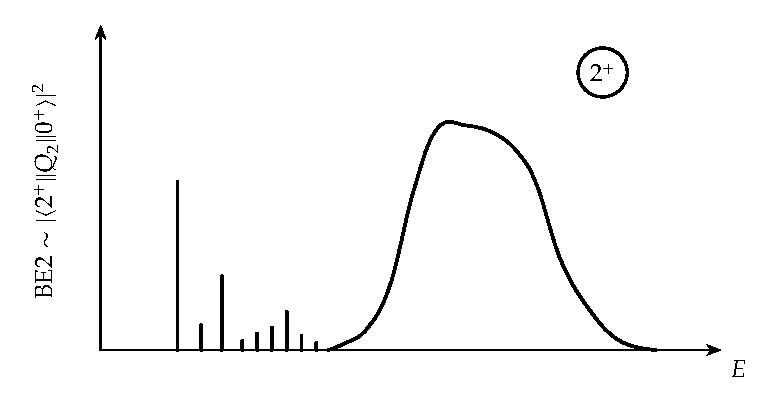
\includegraphics[width=0.75\linewidth]{pictures/1_6}
\par\end{centering}
\centering{}\caption{\label{fig:1_6}原子核中$2^{+}$能谱的示意图。纵坐标给出离散能级的$BE2$值以及共振区中的$BE2$强度密度。这些量表征向基态跃迁的概率。单位是任意的。}
\end{figure}

因此，低激发$2^{+}$态具有集体性质，即由许多粒子协同贡献，且常常被解释为表面四极振动。\ref{fig:1_7}给出了偶偶核中最低$2^{+}$态的能量$E_{2^{+}}$。可以观察到显著的壳效应（见第
2 章）。基于无旋流假设的液滴模型 {[}式 (1.19)、(1.30) 与 (1.34){]} 仅能给出平均趋势，其绝对值相差约
5 倍。

在实验上发现，第一$2^{+}$态的$BE2$值与其能量$E_{2^{+}_{1}}=\hbar\Omega_{2}$之间存在强烈的关联
\cite{Gr62}：
\begin{equation}
E_{2^{+}_{1}}B(E2,2^{+}\rightarrow0^{+})\simeq(25\pm8)\frac{Z^{2}}{A}\,[\text{MeV}\cdot e^{2}\cdot\text{fm}^{4}].\label{eq:1.40}
\end{equation}
这一经验关系在整个核素图的所有原子核中均成立。式 (1.39) 表现出相同的能量依赖性，但其对质量数$A$的依赖关系有所不同。低激发$2^{+}$态中显著的壳效应表明，它们不可能仅仅是纯粹的四极表面振荡，并且还存在具有这种集体振动性质的其他状态。由式
(1.22)、(1.21) 和 (1.35) 可见，四极表面振动在$\alpha$的线性阶下可表示为：
\begin{equation}
|2\mu)=B^{\dagger}_{2\mu}|0\rangle\propto\hat{\alpha}_{2\mu}|0\rangle\propto\hat{Q}_{2\mu}|0\rangle.\label{eq:1.41}
\end{equation}
因此，任意态$|\nu\rangle$与四极表面振动态的重叠正比于其$BE2$值：
\begin{equation}
|\langle\nu|2\mu\rangle|^{2}\propto|\langle\nu|\hat{Q}_{2\mu}|0\rangle|^{2}\propto B(E2,\nu\rightarrow0),\label{eq:1.42}
\end{equation}
而该态能被解释为这种振动的概率，由其耗尽求和规则的百分比给出：
\begin{equation}
S^{0}_{2\mu}=\sum_{\nu\neq0}|\langle\nu|\hat{Q}_{2\mu}|0\rangle|^{2}.\label{eq:1.43}
\end{equation}
只有当某个态在很大程度上耗尽了此求和规则时，将其称为四极表面振动才有明确的物理意义。

\begin{figure}[H]
\begin{centering}
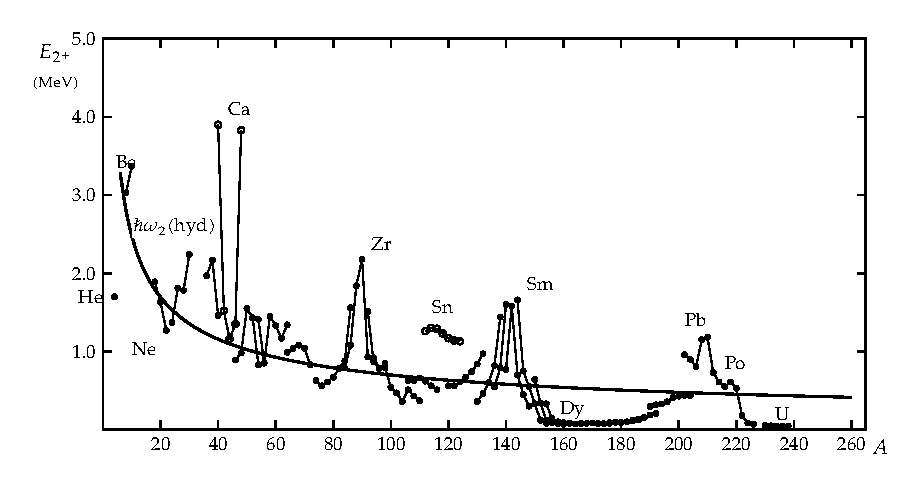
\includegraphics[width=0.85\linewidth]{pictures/1_7}
\par\end{centering}
\centering{}\caption{\label{fig:1_7}偶偶核中第一$2^{+}$态的能量。中子或质子为闭壳的核用空心圆圈标记（引自 \cite{NN65}）。}
\end{figure}

在 8.7 节中，我们将详细讨论求和规则及其计算方法。显而易见，在我们当前研究的模型中，态$\hat{Q}_{\lambda\mu}|0\rangle$是系统的本征态，因此该态完全耗尽了求和规则，因为所有其他态都与它正交。

在实验上发现，低激发$2^{+}$态通常仅耗尽求和规则的约 $10\%\sim20\%$。其主要部分被连续谱中的共振态所耗尽 {[}参见\ref{fig:1_6}{]}，即所谓的巨共振（giant
resonances）。

实验上已经观测到了具有不同自旋$I$的巨共振。最著名的便是巨偶极共振（$1^{-}$），三十多年来已广为人知，其能量位于（参见\ref{fig:1_8}，更详细讨论见第
13 章）：
\begin{equation}
\Omega^{\text{GR}}_{1}\simeq77\cdot A^{-1/3+-1/6}\,[\text{MeV}].\label{eq:1.44}
\end{equation}
正如我们将在第 8 章和第 13 章中看到的，它对应于中子球与质子球彼此相对的相对振动，无法在当前的简单模型中加以描述。

在近十年中，人们观测到了更多的巨共振。最重要的例子是同位旋标量巨四极共振。它所处的能量约为（参见\ref{fig:1_8}）：
\begin{equation}
\Omega^{\text{GR}}_{2^{+}}\simeq62\cdot A^{-1/3}\,[\text{MeV}],\label{eq:1.45}
\end{equation}
并且在多数情形下耗尽了$S_{2^{+}}$求和规则的大部分。

因此，将此共振解释为迄今所讨论的四极表面振动模似乎更为合理。然而，目前这种形式的液滴模型无法给出正确的质量数$A$依赖性。由式 (1.19)、(1.30)
和 (1.34) 可得
\[
\Omega_{2}\propto A^{-1/2},
\]
这与实验值 (1.45) 并不一致。在第 13 章中我们将看到，出现该偏差的原因在于：势能系数$C_{\lambda}$对应于液滴的总结合能
{[}(1.31)、(1.34){]}。然而，这一总结合能是内秉动能与势能之和。在式 (1.34) 中忽略了内秉动能（至少对小形变而言）对形变的依赖性。这可以简单理解为核子长平均自由程与不确定性原理的共同效应：不确定性原理指出，在椭球形状中，核子沿短轴方向的动量高于沿长轴方向的动量。然而，椭球形的动量分布比球形动量分布产生更大的动能。由于所有粒子均受到影响，这是一种体积效应，通常压倒了式
(1.34) 中给出的表面依赖性。在第 13 章中，我们将对这一点展开详细讨论。

\begin{figure}[H]
\begin{centering}
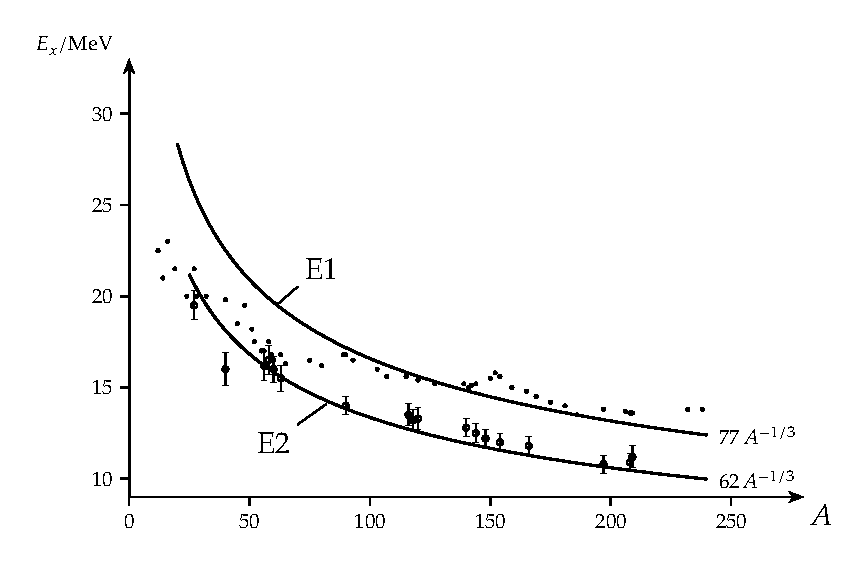
\includegraphics[width=0.75\linewidth]{pictures/1_8}
\par\end{centering}
\centering{}\caption{\label{fig:1_8}巨偶极共振与同位旋标量巨四极共振能量随质量数的变化关系 \cite{Wa73}。}
\end{figure}

尽管存在这些不足，但迄今为止所介绍的玻色子模型多年来仍得到了广泛应用，并在解释核谱的许多特征方面被证明相当成功 \cite{EG70}。其原因在于：许多低激发核态具有相当强的集体性质，可以很好地近似表示为玻色子。参数$B_{\lambda}$和$C_{\lambda}$在液滴模型中或许未能得到很好的给出，但正如我们将在第
8 章和第 9 章中所展示的，存在基于费米子的微观理论能够对$B_{\lambda}$和$C_{\lambda}$进行更为可靠的计算；因此，我们更应当将$B_{\lambda}$和$C_{\lambda}$视作开放的待定可调参数，而非由液滴模型所唯一决定。

微观理论还将表明，简谐近似 (1.17) 仅在极小振动的极限下具有非常粗略的有效性。对于具有较大振幅的集体运动，人们必须考虑非简谐项，例如
\[
\alpha^{4},\,\alpha^{2}\cdot\dot{\alpha}^{2},\,\dot{\alpha}^{4},\,\dots
\]
同样地，相应的参数既可以通过拟合实验来确定，也可以由微观多体理论计算得出（参见第 9 章）。

\section{形变的转动和振动\label{sec:=005F62=0053D8=007684=008F6C=0052A8=00548C=00632F=0052A8}\label{sec:1.5_=008F6C=0052A8=005E26}}

\subsection{Bohr Hamilton量\label{subsec:Bohr-Hamilton=0091CF}}

纯液滴模型仅在球形表面时具有稳定平衡。正如我们稍后将看到的（第 2.8 节），量子力学效应——即壳效应——可能导致集体 Hamilton
量中的势能$V(\boldsymbol{\alpha})$在有限非零值$\boldsymbol{\alpha}=\boldsymbol{\alpha}_{0}$处出现极小值。在此类情形下，原子核在基态即可具有稳定的形变。

在这种情况下，原子核可以展现出转动运动，该转动在实验室参考系中可由含时的表面参数$\alpha_{\lambda\mu}$来描述。我们将这些转动称为集体转动。绕对称轴的这种转动是不可能的，因为在我们的变量$\alpha_{\lambda\mu}$中，无法将转动后的系统与原始系统区分开来。

在量子力学描述中，具有对称轴（例如$z$轴）的系统由角动量算符$J_{z}$的本征波函数所描述，绕该对称轴的任何转动仅产生一个相位因子。因此，转动系统具有与基态相同的波函数和相同的能量。

这并不意味着系统中不存在其他可被激发并沿平行于对称轴方向携带角动量的自由度（例如单粒子自由度）。然而，这样一种“转动”我们并不称之为集体转动。

由于在几乎所有原子核中，四极自由度都起着根本性的作用，我们在下文中将把讨论局限于$\lambda=2$的情形。

假定原子核具有稳定的基态形变，最好将其变换到由质量分布主轴所定义的体固参考系中（如 1.3 节所讨论）。

完成该变换后，我们拥有五个动力学变量$\Omega$、$\beta$、$\gamma$\footnote{遗憾的是，Euler 角集合$\Omega=(\alpha,\beta,\gamma)$中也包含了字母$\beta$和$\gamma$。然而，我们不想改变这一通用命名习惯
\cite{Ed57}，因此尽可能采用缩写记号$\Omega$。}，用以代替原先的五个变量$\alpha_{2\mu}\,(\mu=-2,-1,0,+1,+2)$。我们再次从 Hamilton 量
(1.17) 出发，其中仅势能项发生改变，它现在的形式为：
\begin{equation}
V(\beta,\gamma)=\frac{1}{2}C_{20}(a_{20}(\beta,\gamma)-a^{0}_{20})^{2}+C_{22}(a_{22}(\beta,\gamma)-a^{0}_{22})^{2}.\label{eq:1.46}
\end{equation}
这对应于形变极小值$\beta_{0},\gamma_{0}$邻域内的二次近似。其物理图像是：原子核在其基态下具有这一形变，而激发态则是围绕此平衡形变的转动与小振动。

势能面的微观计算表明，对于某些特定的原子核，势能$V$在有限值$\beta_{0}\simeq0.2\sim0.3$以及$\gamma_{0}=0$处具有非常明显的极小值。因此，这些轴对称形状是最重要的情形，我们讨论的大部分内容都将针对它们展开。

下一步是将式 (1.17) 中的动能项变换到体固参考系。应用式 (1.11)，我们必须对变量$a_{20}$、$a_{22}$和$\Omega$对时间求导。由于该推导过程相当繁琐，且本章的目的并非包罗万象，我们仅给出所谓的
Bohr Hamilton 量 \cite{Bo52} 的结果（有关推导细节，参见例如 \cite[第 I 卷第 5 章]{EG70}）：
\begin{equation}
T=T_{\text{rot}}+\frac{1}{2}B_{2}(\dot{\beta}^{2}+\beta^{2}\dot{\gamma}^{2}),\label{eq:1.47}
\end{equation}
其中
\begin{equation}
T_{\text{rot}}=\frac{1}{2}\sum^{3}_{\kappa=1}\mathcal{J}_{\kappa}\omega^{2}_{\kappa},
\end{equation}
这里$\omega_{\kappa}$为绕体固$\kappa$轴的转动角速度，而$\mathcal{J}_{\kappa}$是由下式给出的$\beta$和$\gamma$的函数：
\begin{equation}
\mathcal{J}_{\kappa}=4B_{2}\beta^{2}\sin^{2}\left(\gamma-\frac{2\mathrm{\pi}}{3}\kappa\right),\quad\kappa=1,2,3.\label{eq:1.48}
\end{equation}
在我们固定形变$\beta,\gamma$的情形下，$T_{\text{rot}}$即为转动惯量为$\mathcal{J}_{\kappa}$的转子的动能。一旦我们允许$\beta$和$\gamma$发生变化，转动和振动自由度就会通过转动惯量对形变的依赖性耦合在一起。在这种情况下，我们不再拥有一个纯粹的转子。事实上我们看到，在$\beta_{0}=0$的情况下，该系统可以变换回具有谐振子谱的简谐振子
(1.17)。

然而，即使在具有较大刚度参数$C$和有限$\beta_{0}$的强形变情形下（此时常数近似$\beta=\beta_{0}$是相当好的近似），$\mathcal{J}_{\kappa}$也并不是刚体转子的转动惯量。利用式
(1.30)，我们由式 (1.48) 得到所谓的无旋流转动惯量：
\[
\mathcal{J}^{\text{irr}}_{\kappa}=\frac{3}{2\mathrm{\pi}}mAR^{2}_{0}\beta^{2}\sin^{2}\left(\gamma-\frac{2\mathrm{\pi}}{3}\kappa\right),\quad\kappa=1,2,3.
\]
它与具有相同形变的刚体转动惯量
\begin{equation}
\mathcal{J}^{\text{rig}}_{\kappa}=\frac{2}{5}mAR^{2}_{0}\left(1-\sqrt{\frac{5}{4\mathrm{\pi}}}\beta\cos\left(\gamma-\frac{2\mathrm{\pi}}{3}\kappa\right)\right)\label{eq:1.49}
\end{equation}
在以下几个方面存在显著差异：
\begin{enumerate}
\item 在$\gamma$依赖性方面（\ref{fig:1_9}），$\mathcal{J}^{\text{irr}}$在绕对称轴时严格为零。
\item $\mathcal{J}^{\text{irr}}$对形变具有强烈的依赖性（$\sim\beta^{2}$），而$\mathcal{J}^{\text{rig}}$随$\beta$的变化要弱得多（其主要部分是刚体球的转动惯量）。
\item 实验测得的转动惯量$\mathcal{J}^{\text{exp}}$可由转动带第一$2^{+}$态的能量求得 {[}参见式 (1.64){]}。即有$\mathcal{J}^{\text{exp}}=3/E_{2^{+}}$$[\text{MeV}^{-1}]$。结合经验规则
(1.40) 以及关于$BE2$值的公式 (1.74)，我们得到形变参数$\beta$与转动惯量之间的关联：
\begin{align}
\mathcal{J}^{\text{exp}} & =\frac{27}{80\mathrm{\pi}^{2}r^{4}_{0}}\frac{A^{4/3}\cdot\beta^{2}\cdot Z^{2}e^{2}}{E_{2^{+}}\cdot BE2}\approx\frac{27(1.2)^{4}\cdot\beta^{2}A^{7/3}}{80\mathrm{\pi}^{2}\cdot25}\nonumber \\
 & \approx\frac{\beta^{2}A^{7/3}}{400}\,[\text{MeV}^{-1}].\label{eq:1.50}
\end{align}
\end{enumerate}
在强形变核（$\beta\sim0.2\sim0.4$）的情形下，$\mathcal{J}^{\text{irr}}$通常比实验值小
2 到 3 倍。另一方面，$\mathcal{J}^{\text{rig}}$的值又比实验值大约 2 倍：
\begin{equation}
\mathcal{J}^{\text{irr}}<\mathcal{J}^{\text{exp}}<\mathcal{J}^{\text{rig}}.\label{eq:1.51}
\end{equation}
这表明原子核内部的流动结构绝非无旋流。另一方面，它也并非刚体转子。

接下来的步骤是对经典 Hamilton 量 (1.47) 进行量子化。众所周知，在一般情况下，经典 Hamilton 量的量子化并不存在唯一的法则
\cite{Me61}。这种不确定性源自不可对易算符排序的自由度\footnote{有关量子化问题的讨论与文献列表见 \cite{MD73}。}。通常人们采用
Pauli 法则 \cite{Pa33}，即在曲线坐标系中计算 Laplace 算符。若经典动能具有如下形式：
\begin{equation}
T=\frac{1}{2}\sum_{ij}g_{ij}(\boldsymbol{\xi})\dot{\xi}_{i}\dot{\xi}_{j},\label{eq:1.52}
\end{equation}

\begin{figure}[H]
\begin{centering}
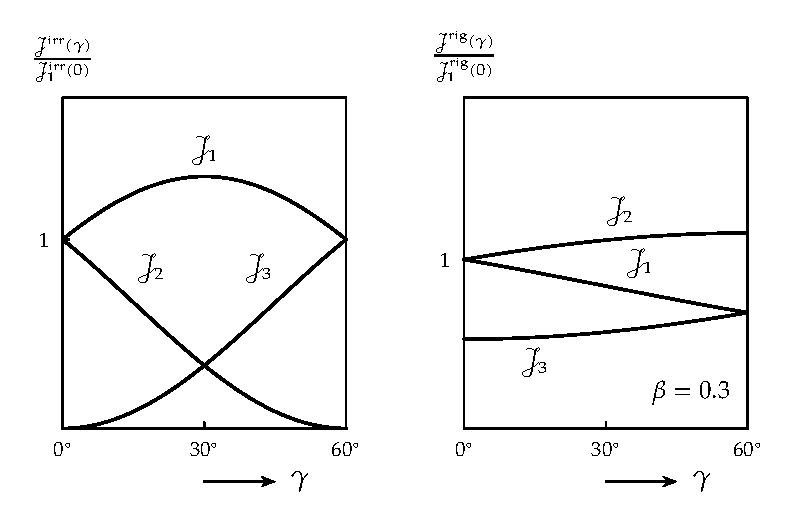
\includegraphics[width=0.75\linewidth]{pictures/1_9}
\par\end{centering}
\centering{}\caption{\label{fig:1_9}在固定的$\beta$值下，无旋流转动惯量（$\mathcal{J}^{\text{irr}}_{\kappa}$）与刚体转动惯量（$\mathcal{J}^{\text{rig}}_{\kappa}$）对$\gamma$的依赖关系。}
\end{figure}

则相应的量子化形式为\footnote{为了看清 Hamilton 量 (1.53) 是厄米的，必须计入体积元$\sqrt{g}\,\mathrm{d}\xi_{1}\dots\mathrm{d}\xi_{f}$。}：
\begin{equation}
\hat{H}_{\text{kin}}=-\frac{\hbar^{2}}{2}\sum_{ij}g^{-1/2}\frac{\partial}{\partial\xi_{i}}g^{1/2}(g^{-1})_{ij}\frac{\partial}{\partial\xi_{j}},\label{eq:1.53}
\end{equation}
其中$g$为矩阵$g_{ij}$的行列式，而$g^{-1}$为其逆矩阵。

将此法则应用于 Bohr Hamilton 量 (1.46) 和 (1.47)，我们得到：
\begin{align}
\hat{H}_{\text{coll}} & =-\frac{\hbar^{2}}{2B_{2}}\left[\beta^{-4}\frac{\partial}{\partial\beta}\left(\beta^{4}\frac{\partial}{\partial\beta}\right)+\frac{1}{\beta^{2}\sin3\gamma}\frac{\partial}{\partial\gamma}\left(\sin3\gamma\frac{\partial}{\partial\gamma}\right)\right]\nonumber \\
 & \quad+\hat{T}_{\text{rot}}+V(\beta,\gamma),\label{eq:1.54}
\end{align}
其中转动能为
\begin{equation}
\hat{T}_{\text{rot}}=\frac{\hat{I}^{2}_{1}}{2\mathcal{J}_{1}}+\frac{\hat{I}^{2}_{2}}{2\mathcal{J}_{2}}+\frac{\hat{I}^{2}_{3}}{2\mathcal{J}_{3}}.\label{eq:1.55}
\end{equation}
算符$\hat{I}_{\kappa}$为用 Euler 角表示的总角动量$\hat{\boldsymbol{I}}$在体固坐标轴上的投影（细节参见附录
A）。\ref{fig:1_10}展示了总角动量及其分量$\hat{I}_{z}=M$与$\hat{I}_{3}=K$。算符$\hat{\boldsymbol{I}}^{2}$、$\hat{I}_{z}$、$\hat{I}_{3}$的共同本征函数由下式给出：
\begin{equation}
|IMK\rangle=\sqrt{\frac{2I+1}{8\mathrm{\pi}^{2}}}D^{I*}_{MK}(\Omega).\label{eq:1.56}
\end{equation}
由于$H_{\text{coll}}$、$\hat{\boldsymbol{I}}^{2}$与$\hat{I}_{z}$彼此对易，集体
Hamilton 量的本征函数具有一般形式：
\[
|\Psi^{I}_{M}\rangle=\sum_{K}g_{K}(\beta,\gamma)|IMK\rangle.
\]

\begin{figure}[H]
\begin{centering}
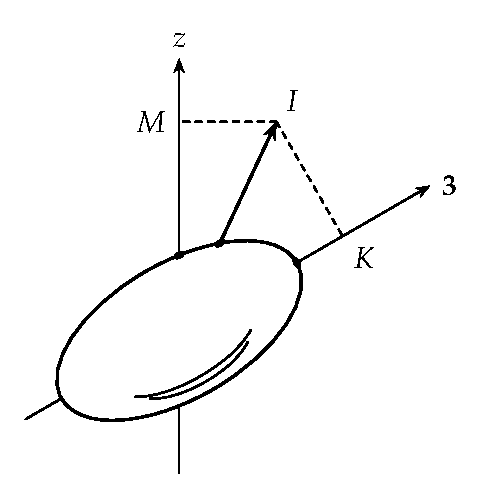
\includegraphics[width=0.75\linewidth]{pictures/1_10}
\par\end{centering}
\centering{}\caption{\label{fig:1_10}总角动量$I$与其在实验室$z$轴上的投影$M$以及在体固 3 轴上的投影$K$之间的关系。}
\end{figure}

三轴转子具有特定的离散对称性。$\hat{H}_{\text{coll}}$在点群$D_{2}$变换下保持不变 \cite{Bo52}。因此，可以根据该群的不可约表示对本征态进行分类，并由此推导出发射谱的若干性质
\cite{Da68}。

一个例子是绕 1 轴转动$180^{\circ}$的操作：
\begin{equation}
\mathscr{R}_{1}=\mathrm{e}^{\mathrm{i}\mathrm{\pi}\hat{I}_{1}},\label{eq:1.57}
\end{equation}
这等价于对 2, 3 平面的反射与宇称变换的复合。它与$\hat{H}_{\text{coll}}$对易，我们要求本征函数具有本征值$+1$\footnote{正如我们将在式 (11.123) 中看到的，系统的微观内秉波函数是该操作本征值为$+1$的本征态（亦参见 \cite{Bo76b}）。}：
\begin{equation}
\mathscr{R}_{1}|\Psi^{I}_{M}\rangle=|\Psi^{I}_{M}\rangle.\label{eq:1.58}
\end{equation}
利用附录 A 中的关系式 (A.24)，我们发现这仅在满足下述条件时才可能成立：
\begin{equation}
g_{K}(\beta,\gamma)=(-)^{I}g_{-K}(\beta,\gamma).\label{eq:1.59}
\end{equation}
同理，若我们要求对如下转动的对称性：
\begin{equation}
\mathscr{R}_{2}=\mathrm{e}^{\mathrm{i}\mathrm{\pi}\hat{I}_{2}},\label{eq:1.60}
\end{equation}
则得到
\begin{equation}
g_{K}(\beta,\gamma)=(-)^{I+K}g_{-K}(\beta,\gamma).\label{eq:1.61}
\end{equation}


\subsection{轴对称情形\label{subsec:=008F74=005BF9=0079F0=0060C5=005F62}}

Hamilton 量$\hat{H}_{\text{coll}}$ (1.54) 仍然非常一般。我们在此将限制于势能面在轴对称形变$\beta=\beta_{0}$和$\gamma=0$处具有非常显著极小值的情形。我们预期核表面会出现转动和小振动。将式
(1.55) 中的$T_{\text{rot}}-\hat{I}^{2}_{3}/2\mathcal{J}_{3}$围绕点$\beta=\beta_{0},\gamma=0$展开，在零阶近似下我们得到转动惯量为$\mathcal{J}_{0}=\mathcal{J}_{1}(\beta_{0},0)=\mathcal{J}_{2}(\beta_{0},0)$的轴对称转子的
Hamilton 量：
\begin{equation}
T^{\prime}_{\text{rot}}=\frac{\hat{\boldsymbol{I}}^{2}-\hat{I}^{2}_{3}}{2\mathcal{J}_{0}}.\label{eq:1.62}
\end{equation}
一阶项正比于偏离量$(\beta-\beta_{0})$与$\gamma$。它们使转动与振动自由度相混合（转动-振动耦合项），在此处予以略去。在$H_{\text{coll}}$中仍然耦合转动与振动的唯一项是$\hat{I}^{2}_{3}/2\mathcal{J}_{3}$。由于$\mathcal{J}_{3}$在$\gamma=0$时为零，该项不能被展开。然而（如同$T^{\prime}_{\text{rot}}$），它与$\hat{I}_{3}$对易，因此$K$是一个好量子数。

我们现在必须区分两种情形：

\paragraph*{(i) $K=0$ 带（$I_{3}=0$）。}

在这种情况下，转动与振动运动解耦。波函数具有如下形式：
\begin{equation}
|\Psi^{I}_{M0}\rangle=g_{0}(\beta,\gamma)|IM0\rangle.\label{eq:1.63}
\end{equation}
它们是 Hamilton 量 (1.54) 转动部分的本征函数。$\mathscr{R}_{1}$对称性 (1.59) 要求自旋序为$I=0,2,4,\dots$。对$H_{\text{coll}}$振动部分的详细研究
\cite[第 I 卷第 6 章]{EG70} 表明，在变量$a_{20}$和$a_{22}$ (1.13)
下处理更为简便。在第一步中，人们略去势能$V(a_{20},a_{22})$中将这两个自由度耦合起来的交叉项。在此情形下，沿坐标$a_{20}$的运动（通常称为$\beta$振动）与沿坐标$a_{22}$的运动（通常称为$\gamma$振动）解耦。绕
3 轴的轴对称性在$\beta$振动（量子数为$n_{\beta}$）下得以保持，但在$\gamma$振动（量子数为$n_{\gamma}$）下被破坏。\ref{fig:1_11}定性地展示了这两种运动形式。

叠加在每个振动态$(n_{\beta},n_{\gamma})$之上的是一个转动带。其能谱由下式给出（参见 \cite[第 I 卷第 6 章]{EG70}）：
\begin{equation}
E_{n_{\beta}n_{\gamma}}(I)=E_{n_{\beta}n_{\gamma}}(0)+\frac{\hbar^{2}}{2\mathcal{J}_{0}}I(I+1),\label{eq:1.64}
\end{equation}
其带头能量为：
\begin{equation}
E_{n_{\beta}n_{\gamma}}(0)=\hbar\omega_{\beta}\left(n_{\beta}+\frac{1}{2}\right)+\hbar\omega_{\gamma}(2n_{\gamma}+1),\quad n_{\beta}=0,1,2,\dots,\quad n_{\gamma}=0,1,2,\dots,\label{eq:1.65}
\end{equation}
其中$\omega_{\beta}$和$\omega_{\gamma}$分别为$\beta$振动和$\gamma$振动的频率：
\[
\omega_{\beta}=(C_{20}/B_{2})^{1/2},\quad\omega_{\gamma}=(C_{22}/B_{2})^{1/2}.
\]
事实上，在许多偶偶核中都观测到了这样的能带，特别是基态带（$n_{\beta}=n_{\gamma}=0$）与“$\beta$带”（$n_{\beta}=1,n_{\gamma}=0$）。然而，正如我们前面所讨论的，流体动力学模型给出的常数$\mathcal{J}_{0}$以及$\omega_{\beta},\omega_{\gamma}$与实验数据并不相符。

\paragraph*{(ii) $K\protect\neq0$ 带。}

结合$\mathscr{R}_{1}$对称性 {[}式 (1.58){]}，我们看到此时波函数具有如下形式：
\begin{equation}
|\Psi^{I}_{MK}\rangle=g_{K}(\beta,\gamma)\frac{1}{\sqrt{2}}\left(|IMK\rangle+(-)^{I}|IM-K\rangle\right).\label{eq:1.66}
\end{equation}
$\mathscr{R}_{1}$与$\mathscr{R}_{2}$对称性（式 (1.59) 和 (1.61)）给出了选择定则：$K$必须为偶数。因此，这样的$K\neq0$带具有自旋序列$I=|K|,|K|+1,|K|+2,\dots$。沿$a_{20}$的运动（$\beta$振动）同样可以与其余部分分离。然而，项$\hat{I}^{2}_{3}/2\mathcal{J}_{3}=K^{2}/16B_{2}a^{2}_{22}$将$\gamma$振动与绕
3 轴的转动耦合在一起。如果我们认识到$\gamma$振动可以表示为三轴核绕 3 轴以相反$K$值进行的两次转动的叠加，就很容易理解这一事实
\cite[第 656 页]{BM75}。

由此得到如下能谱 \cite[第 I 卷第 6 章]{EG70}：
\begin{equation}
E_{K,n_{\beta},n_{\gamma}}(I)=E_{K,n_{\beta},n_{\gamma}}(0)+\frac{\hbar^{2}}{2\mathcal{J}_{0}}(I(I+1)-K^{2}),\label{eq:1.67}
\end{equation}

\begin{figure}[H]
\begin{centering}
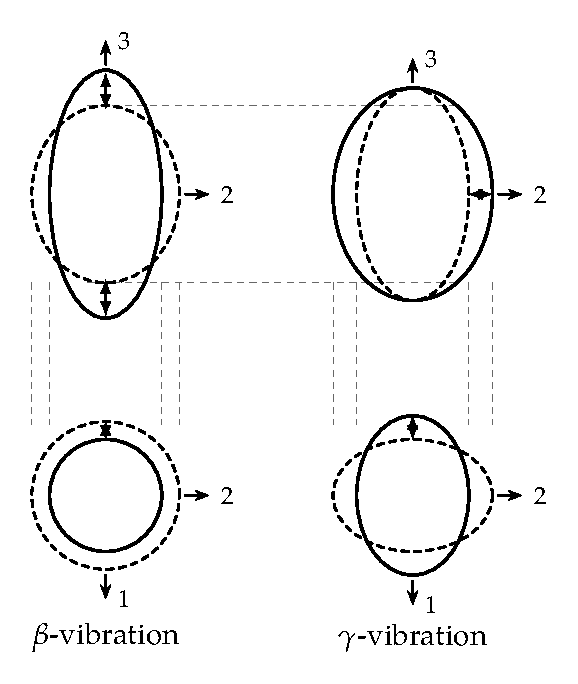
\includegraphics[width=0.75\linewidth]{pictures/1_11}
\par\end{centering}
\centering{}\caption{\label{fig:1_11}通过沿 (1, 3) 与 (1, 2) 平面剖切示意性表示的$\beta$振动与$\gamma$振动。}
\end{figure}

其带头能量为：
\begin{equation}
E_{K,n_{\beta},n_{\gamma}}(0)=\hbar\omega_{\beta}\left(n_{\beta}+\frac{1}{2}\right)+\hbar\omega_{\gamma}\left(2n_{\gamma}+1+\frac{|K|}{2}\right).\label{eq:1.68}
\end{equation}
事实上，这类能带也已被观测到，特别是在许多形变核中具有量子数$K=2,n_{\beta}=0,n_{\gamma}=0$的所谓“$\gamma$带”。虽然该$\gamma$带的振动量子数为$n_{\gamma}=0$，但在此情形下绝不能套用无振动的经典图像。因为经典无振动图像对应于$\gamma=0$，从而意味着$\mathcal{J}_{3}=0$，这将禁戒$K\neq0$的转动。正是量子力学在$\gamma$方向上的零点振动才使得这种激发成为可能。

\ref{fig:1_12}给出了形变核与球形核中集体（$\lambda=2$）激发的定性结构。

球形核具有简谐谱。在形变核中，我们观察到建立在基态、$\beta$振动态（$K=0,n_{\beta}=1,n_{\gamma}=0$）以及$\gamma$振动态（$K=2,n_{\beta}=0,n_{\gamma}=0$）之上的若干转动带。然而，这些纯粹的情形在自然界中并未严格实现。事实上，我们已经在球形核中观察到了双玻色子三重态（$0^{+},2^{+},4^{+}$）的劈裂，并在形变核中观察到了对$I(I+1)$规律的偏离。在两个极限之间还存在着大范围的过渡核。从一种同位素到另一种同位素，人们有时可以观察到从振动谱到转动谱的平滑过渡（例如在
Os 区核中 \cite{SDG76}）。这在\ref{fig:1_12}中用虚线示意给出。

\begin{figure}[H]
\begin{centering}
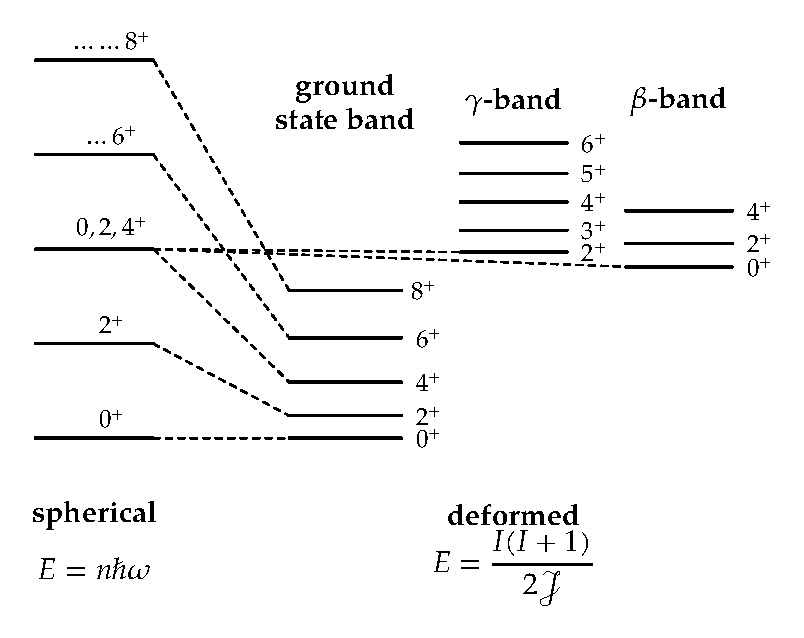
\includegraphics[width=0.75\linewidth]{pictures/1_12}
\par\end{centering}
\centering{}\caption{\label{fig:1_12}球形核与形变核能级方案的示意图（引自 \cite{SDG76}）。}
\end{figure}

为了从理论上描述对$I(I+1)$规律的偏离，人们考虑了$\hat{H}_{\text{coll}}$中的转动-振动耦合项，这些项是通过将$\mathcal{J}_{\kappa}$按偏离量$(\beta-\beta_{0})$和$\gamma$的幂次展开而得到的
\cite{FG62,FG64,FGS65,FGS66,ABP68}。这种转动-振动相互作用引起能带转动惯量的变化，对应于原子核形状在转动影响下的形变拉伸（stretching
effect）。然而，在这一能区内还存在着原子核截然不同的其他激发，例如双准粒子态和配对振动（参见第 8 章），它们对转动带的影响要强得多，而这些在带有表面振动的简单液滴模型中并未加以考虑。

在结束本节之前，我们简要讨论如何计算电磁极矩和跃迁概率。在式 (1.35) 和 (1.36) 中，我们利用坐标$\alpha_{\lambda\mu}$定义了电多极矩和磁偶极矩算符。它们显然是在实验室坐标系中写出的。在形变核中，在内秉参考系中计算极矩通常极为方便。为了得到实验室参考系中的极矩——即实验测得的值——必须应用球张量的变换关系
(1.11)：
\begin{equation}
\hat{Q}^{\text{intr}}_{\lambda\mu}=\sum_{\mu^{\prime}}D^{\lambda}_{\mu^{\prime}\mu}\hat{Q}^{\text{lab}}_{\lambda\mu^{\prime}}.\label{eq:1.69}
\end{equation}
由于$Q^{\text{intr}}$不依赖于 Euler 角，根据 \cite[式 4.6.2 和 5.4.1]{Ed57}，我们得到在基底$|IMK\rangle$下的约化矩阵元：
\begin{equation}
\langle I_{1}K_{1}||\hat{Q}^{\text{lab}}_{\lambda}||I_{2}K_{2}\rangle=\sum_{\mu^{\prime}}Q^{\text{intr}}_{\lambda\mu^{\prime}}(-)^{I_{1}-K_{1}}((2I_{1}+1)(2I_{2}+1))^{1/2}\begin{pmatrix}I_{1} & \lambda & I_{2}\\
-K_{1} & \mu^{\prime} & K_{2}
\end{pmatrix}.\label{eq:1.70}
\end{equation}
我们现在限制于纯$K$带，且仅计算带内$E2$跃迁（$n_{\gamma_{1}}=n_{\gamma_{2}},n_{\beta_{1}}=n_{\beta_{2}}$）。对于约化矩阵元，我们求得：
\begin{equation}
\langle n_{\beta}n_{\gamma}I_{1}K||\hat{Q}^{\text{lab}}_{2}||n_{\beta}n_{\gamma}I_{2}K\rangle=\sqrt{\frac{5}{16\mathrm{\pi}}}Q_{0}(n_{\beta},n_{\gamma})\sqrt{(2I_{1}+1)(2I_{2}+1)}(-)^{I_{1}-K}\begin{pmatrix}I_{1} & 2 & I_{2}\\
-K & 0 & K
\end{pmatrix},\label{eq:1.71}
\end{equation}
其中$Q_{0}(n_{\beta},n_{\gamma})$为该能带的内秉四极矩。在固定$\beta$值且$\gamma=0$的基态带中，由式
(1.13) 和 (1.35) 可得：
\begin{equation}
Q_{0}=\sqrt{\frac{16\mathrm{\pi}}{5}}\frac{3}{4\mathrm{\pi}}Ze\cdot R^{2}_{0}\cdot\beta.\label{eq:1.72}
\end{equation}
由式 (B.73) 与 (1.71)，我们例如可以求得转动带中所谓的跨跃（stretched）$BE2$值：
\begin{equation}
B(E2,I+2\rightarrow I)=Q^{2}_{0}\frac{5}{16\mathrm{\pi}}|C^{I+2\,2\,I}_{K\,0\,K}|^{2},\label{eq:1.73}
\end{equation}
对于$K=0$带，该式给出：
\begin{equation}
B(E2,I+2\rightarrow I)=Q^{2}_{0}\frac{5}{16\mathrm{\pi}}\frac{3}{2}\frac{(I+1)(I+2)}{(2I+3)(2I+5)}.\label{eq:1.74}
\end{equation}
对于光谱学四极矩$Q=\sqrt{16\mathrm{\pi}/5}\langle IIK|\hat{Q}^{\text{lab}}_{20}|IIK\rangle$
{[}式 (B.32){]}，我们得到：
\begin{equation}
Q=Q_{0}\frac{3K^{2}-I(I+1)}{(2I+3)(I+1)}.\label{eq:1.75}
\end{equation}
商值$Q:Q_{0}$即为态$M=I$中$D^{2}_{00}=P_{2}(\cos\beta)$的期望值。这意味着人们无法直接测量内秉四极矩$Q_{0}$，而只能测得在转动运动上平均的值。事实上，$Q_{0}$并非一个严格的物理可观测量。它的定义依赖于随原子核共同运动的体固坐标系的引入，具有模型依赖的性质。对于带头通常有$I=K$。这意味着具有$I=0$的基态的光谱学四极矩$Q$为零，我们只能对激发态获得关于$Q_{0}$的信息（例如通过
Coulomb 激发中的重取向效应（reorientation effect）\cite{BE68}，它给出了$Q_{0}$的符号与绝对值）。确定$Q_{0}$绝对值的另一种方法是测量带内跃迁的$B(E2)$值
(1.73)。近年直至高自旋态的测量表明 \cite{WCL76,HJE78}，在许多形变核中，即使能谱显示出对$I(I+1)$特性的偏离，$Q_{0}$的值在这些带内仍保持相当稳定。这提示我们，这些偏离并非由形变的改变（拉伸效应）所主导。

\subsection{非对称转子\label{subsec:=00975E=005BF9=0079F0=008F6C=005B50}}

迄今所讨论的转动-振动相互作用模型均建立在对称转子的基础之上。Davydov 等人利用纯三轴转子的图像进行了进一步尝试，以解释对$I(I+1)$规律的偏离以及许多核中低激发的第二个$2^{+}$态
\cite{DF58,DR59,Da59,Da65b}。作为第一步，他们不考虑振动激发，而仅对转动能 (1.55) 进行对角化。利用转动惯量
(1.48)，该算符正比于$\beta^{-2}$，并且可以针对任意$\gamma$值进行对角化。常数因子随后可通过拟合第一$2^{+}$态来调节。利用对称性$\mathscr{R}_{1}$与$\mathscr{R}_{2}$（式
(1.59) 和 (1.61)），波函数具有如下形式：
\begin{equation}
|\Psi^{I}_{M}\rangle=\sum_{K=0,2,\dots}g_{K}\left\{ |IMK\rangle+(-)^{I}|IM-K\rangle\right\} .\label{eq:1.76}
\end{equation}
\ref{fig:1_13}给出了相应的能量本征值。在$\gamma=0^{\circ}$和$\gamma=60^{\circ}$时，人们得到标准的$I(I+1)$能谱。即使在较强的三轴形变下，对该形式的偏离也微乎其微。然而，额外的$2^{+},3^{+},4^{+}$能级在能量上下降。具有低激发的第二个$2^{+}$态是该结构的显著特征。虽然利用这样一个模型可以相当合理地复现某些元素周期表区域（例如
Os 同位素）的实验数据，但人们仍对它提出了强烈的异议：
\begin{enumerate}
\item 它无法描述$\beta$振动。若要描述$\beta$振动，必须引入额外的振动自由度 \cite{DC60}。
\item 能够确立稳定$\gamma$形变的显著能面极小值迄今尚未被发现。对此类过渡核的微观计算通常显示沿$\gamma$方向只有非常浅的平坦能谷
\cite{KB68,ASS69,GPA72,GG78}\footnote{Wilets 和 Jean \cite{WJ56} 提出了一个完全对$\gamma$软（$\gamma$-soft）的模型，即在式
(1.46) 中设$C_{22}=0$。}。
\end{enumerate}
近年来，稳定的$\gamma$形变重新引起了人们的浓厚兴趣，因为：
\begin{enumerate}
\item 奇$A$过渡核中的实验数据可以通过单粒子耦合于非对称转子的模型得到极好的复现（参见第 5 章以及 \cite{MSD74,Me75,TF75}）。
\item 针对极高自旋态的理论计算表明（参见 1.7 节及 \cite{ALL76}），原子核在特定自旋区域内可能变为三轴形变。
\end{enumerate}
通过假定极大三轴度（$\gamma=30^{\circ}$），人们可以对三轴核的能级结构给出一个粗略的估计。在这种情形下，$\mathcal{J}_{2}=\mathcal{J}_{3}=\frac{1}{4}\mathcal{J}_{1}=\frac{1}{4}\mathcal{J}_{0}$（$\mathcal{J}_{0}$为在$\gamma=0$处的转动惯量），并且（在动能中）我们具有关于
1 轴的对称性。角动量$\boldsymbol{I}$在此轴上的投影$\alpha$是一个好量子数，由此求得：
\begin{equation}
E_{\alpha}(I)=\frac{3\hbar^{2}}{8\mathcal{J}_{0}}(4I(I+1)-3\alpha^{2}).\label{eq:1.77}
\end{equation}

\begin{figure}[H]
\begin{centering}
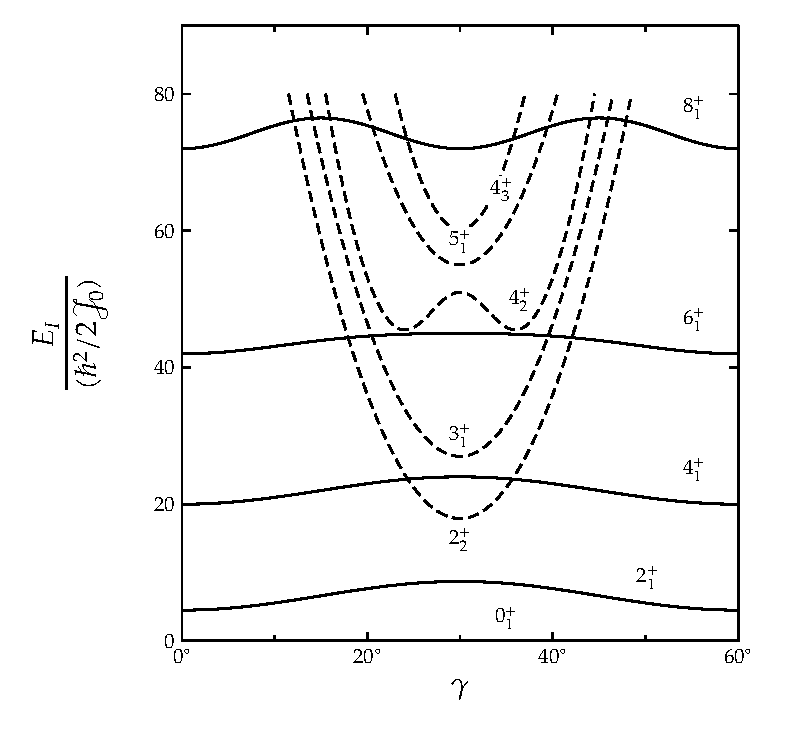
\includegraphics[width=0.75\linewidth]{pictures/1_13}
\par\end{centering}
\centering{}\caption{\label{fig:1_13}具有流体动力学转动惯量的形变非对称转子的能量本征值（引自 \cite{Me75}）。}
\end{figure}

$\mathscr{R}_{1}$与$\mathscr{R}_{2}$对称性要求$I$和$\alpha$均为偶数。对于每个$I$，具有最低能量的能级（即所谓的“yrast”能级）对应于$\alpha=I$。能量次低的能带对应于$\alpha=I-2$，继而是$\alpha=I-4$，依此类推。因此，我们得到了一系列由“摆动”（wobbling）量子数$n=I-\alpha$所表征的能带
\cite{BM75}。可以计算出，具有相同$n$的态之间由很大的$E2$跃迁概率所联接。我们由式 (1.77) 得到它们的能谱：
\begin{equation}
E_{n}(I)=\frac{3\hbar^{2}}{8\mathcal{J}_{0}}(I(I+4)+3n(2I-n)).\label{eq:1.78}
\end{equation}
然而必须牢记，能谱的结构（\ref{fig:1_13}）极度敏感地依赖于转动惯量对$\gamma$的依赖关系。在该图中采用的是流体动力学值。若采用刚体值，能谱的面貌无疑将大为改观。

\section{核裂变\label{sec:=006838=0088C2=0053D8}}

到目前为止，我们在液滴模型中仅研究了围绕平衡形状的小振动。在核裂变被发现后不久，人们便尝试运用核液滴的概念来理解这一现象 \cite{MF39,Fr39,BW39}。

事实上，一个均匀带电的经典液滴，仅在 Coulomb 能不超过某一临界值时才对裂变是稳定的（且保持球形）。Coulomb 排斥倾向于使液滴发生形变，从而使粒子平均而言相距更远。相反，表面能正比于液滴的表面积，倾向于使其保持球形。因此，这两种效应（各自的绝对量级均达数百个
MeV）之间的微妙平衡过程，依据经典计算决定了是否会发生裂变。当然，对于涉及大形变的裂变过程，人们必须超越前几节所讨论的简谐近似 \cite{BW39}。

描述裂变过程的第一步 \cite{HW53} 是选取一组适当的形变参数，我们记作$\boldsymbol{\alpha}$。它必须足够普遍，以能够描述可能出现的所有形变。例如，Cohen
和 Swiatecki \cite{CS62,CS63} 在计算如下形式的对称形状时，考虑了多达 18 阶的多极展开：
\begin{equation}
R=R_{0}\left(1+\sum^{18}_{l=1}\alpha_{l}P_{l}(\cos\theta)\right).\label{eq:1.79}
\end{equation}
这使得人们能够描述非常普遍的几何形状。另一方面，如果人们定性地了解液滴在裂变过程中的演化行为，就会希望引入尽可能少的参数。由于人们还希望描述已分离的碎片，因此参数集
(1.79) 显然不是最合适的。为了对裂变过程进行现实的描述，至少需要三个参数 \cite{NS65,Ni72}：
\begin{enumerate}
\item 参数$c$：在裂变过程开始时在某种意义上描述长半轴的长度，并平滑过渡为已分离碎片之间的间距（伸长坐标，elongation coordinate）；
\item 参数$h$：表征正在形成的碎片之间颈部的厚度（颈部坐标，neck coordinate）；
\item 非对称参数$\alpha_{s}$：度量分离碎片质量分布偏离对称性的程度（在非对称裂变情形下）（碎裂坐标，fragmentation
coordinate）。
\end{enumerate}
\ref{fig:1_14}给出了这种参数化方案的一个实例 \cite{BDJ72}。

\begin{figure}[H]
\begin{centering}
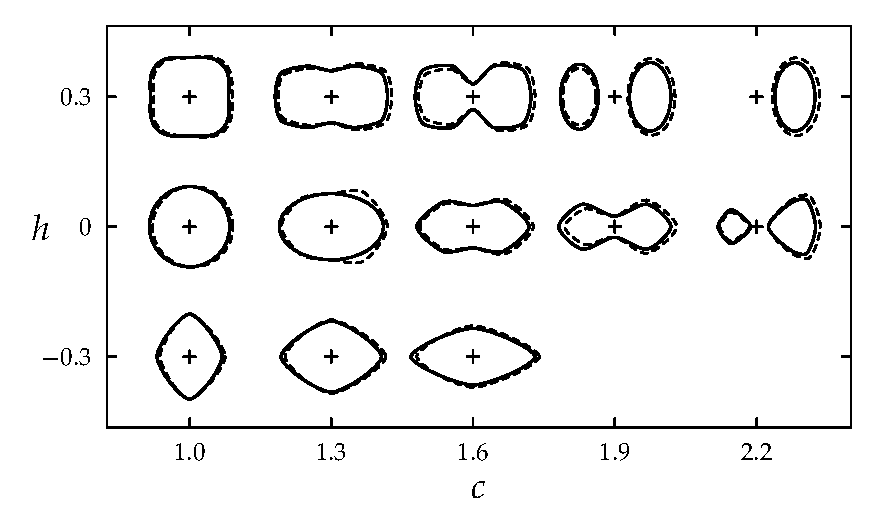
\includegraphics[width=0.85\linewidth]{pictures/1_14}
\par\end{centering}
\centering{}\caption{\label{fig:1_14}在一组适宜的参数化方案$\{c,h\}$下的若干原子核形状。实线表示对称形状；虚线具有非零的非对称参数$\alpha_{s}$（引自
\cite{BDJ72}）。}
\end{figure}

下一步必须计算参数$\boldsymbol{\alpha}$下的 Hamilton 量。首先是势能项$V(\boldsymbol{\alpha})$。人们通常以相应球体的表面能\footnote{如我们前面所讨论的，势能可以具有对应于内秉动能的体积依赖性。然而，对于裂变过程所涉及的大形变，动力学效应对$V(\boldsymbol{\alpha})$可能产生重要影响：通常假定自发裂变过程非常缓慢，以至于核子有充裕的时间调整其动量分布，从而在每个形变下使总能量最小。该动量分布自然是球对称的动量分布。（有关此点的更详细讨论见第
13 章。）}为单位来度量它，得到：
\begin{equation}
V(\boldsymbol{\alpha})=(B_{s}(\boldsymbol{\alpha})-1)+2x(B_{C}(\boldsymbol{\alpha})-1),\label{eq:1.80}
\end{equation}
其中$B_{s}$和$B_{C}$分别为表面能 {[}以$E_{s}(0)$为单位{]} 与 Coulomb 能 {[}以$E_{C}(0)=\frac{3}{5}(eZ)^{2}/R_{0}$为单位{]}。它们的计算类似于式
(1.32) 和 (1.33)。然而，此时人们不能再假定小形变，而必须显式完成各重积分。$B_{s}$和$B_{C}$仅取决于几何形状。表征特定原子核的唯一参数是所谓的可裂变度参数（fissibility
parameter）$x$。我们求得：
\begin{equation}
x=\frac{E_{C}(0)}{2E_{s}(0)}=\frac{Z^{2}/A}{(Z^{2}/A)_{\text{crit}}},\label{eq:1.81}
\end{equation}
其中
\begin{equation}
\left(\frac{Z^{2}}{A}\right)_{\text{crit}}=\frac{40\mathrm{\pi}}{3}\frac{r^{3}_{0}\sigma}{e^{2}}\approx50.\label{eq:1.82}
\end{equation}
Cohen 与 Swiatecki 的计算 \cite{CS62,CS63} 表明，使原子核发生形变最容易的途径是四极形变，且核液滴总体上要么保持球形，要么发生裂变。因此，在零形变处，我们就可以依据势能面$V(\boldsymbol{\alpha})$在原点处沿四极方向的曲率是正还是负，来判定裂变是否发生。然而，这正是我们在考虑
Bohr Hamilton 量 {[}式 (1.17){]} 直至二次项时所已经计算过的。确实，我们看到刚度系数$C_{2}$ {[}式
(1.34){]} 由形变能的表面部分与 Coulomb 部分之差给出，且当满足下式时$C_{2}$开始变为负值 \cite{Wi64}：
\begin{equation}
\frac{Z^{2}}{A}=\left(\frac{Z^{2}}{A}\right)_{\text{crit}}\quad\text{或}\quad x=1.\label{eq:1.83}
\end{equation}
这意味着经典液滴在$Z^{2}/A\lesssim50$或$x<1$时保持稳定且呈球形。对于$x>1$，它立即发生裂变。这一结论可以通过向水银滴上不断增加电荷的实验得到验证。

对于$^{238}\text{U}$，质量公式 (1.4) 给出的 Coulomb 能约为$E_{C}(0)\approx830\,\text{MeV}$，表面能约为$E_{s}(0)\approx520\,\text{MeV}$；因此我们求得可裂变度参数为$x\simeq0.8$，这是该质量区（$230<A<240$）的典型数值。因此，经典液滴模型无法描述自发裂变。实验中观测到的自发裂变完全归因于量子力学的隧穿效应。

液滴的势能面 (1.80) 通常具有非常复杂的结构。对于$x<1$，我们预期存在一个对应于球体的极小值，而在大间距处存在对应于不同碎裂通道的出射能谷
\cite{NS65,Ni69,MN76}。

例如，若仅考虑对称裂变，针对两个参数$c$和$h$，我们得到如\ref{fig:1_15}所示的能量面。可以看到，它形成了一个定义明确的鞍点（saddle）。在鞍点外侧，形变能急剧下降。

\begin{figure}[H]
\begin{centering}
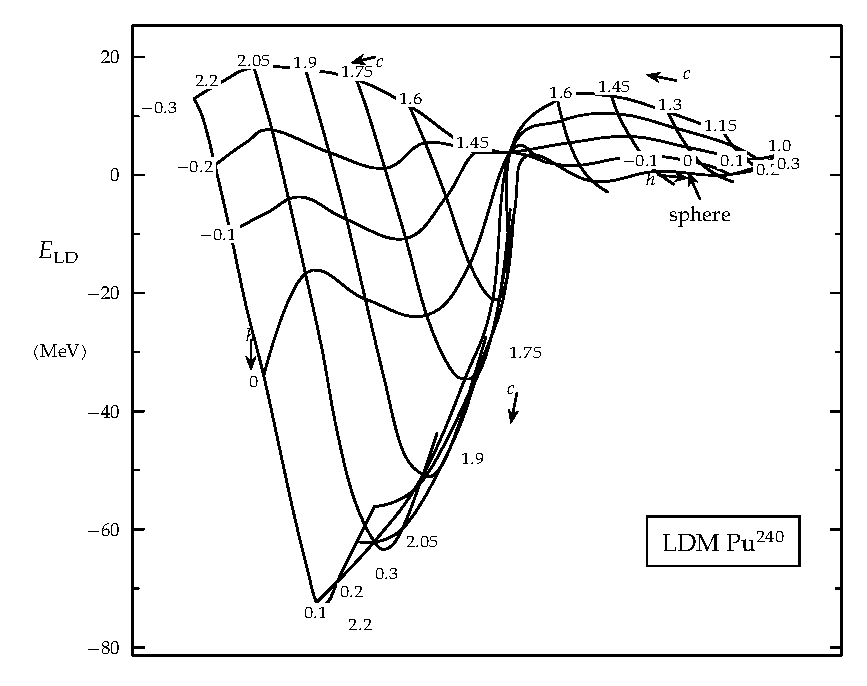
\includegraphics[width=0.85\linewidth]{pictures/1_15}
\par\end{centering}
\centering{}\caption{\label{fig:1_15}$^{240}\text{Pu}$ 液滴模型能量面的透视图。$h$ 描述伸长自由度，$c$
描述颈缩自由度（引自 \cite{BDJ72}）。}
\end{figure}

Cohen 和 Swiatecki \cite{CS63} 利用拟设 (1.79) 计算了许多$x$值下的鞍点形状，其中一部分展示在\ref{fig:1_16}中。

这些鞍点形状的物理含义是：对于给定的$x$，粗略地说，如果使液滴的伸长量比鞍点稍微再大一点，它就不可避免地滑向裂变；反之，若使其伸长量稍微缩短一点，它就会回弹回球形形状。沿着最陡下降线越过鞍点，裂变谷的“谷底”定义了一条一维路径。沿着这条路径的弧长通常称为裂变坐标$s$。\ref{fig:1_17}示意性地展示了沿该坐标的势能分布。

\begin{figure}[H]
\begin{centering}
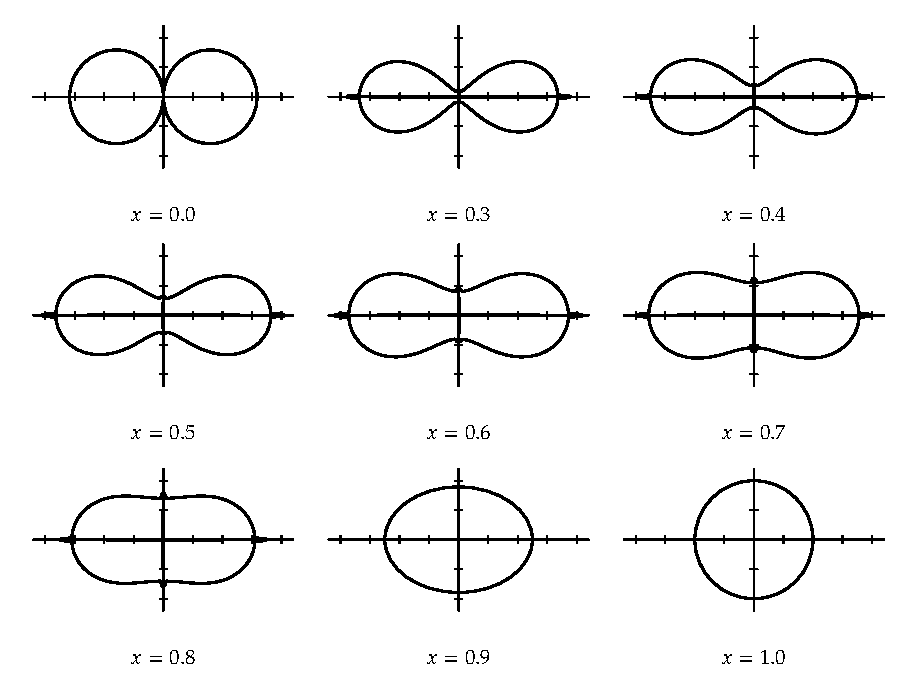
\includegraphics[width=0.85\linewidth]{pictures/1_16}
\par\end{centering}
\centering{}\caption{\label{fig:1_16}可裂变度参数$x$取不同值时的鞍点形状（引自 \cite{CS63}）。}
\end{figure}

裂变势垒高度$E_{B}$通常只有几个 MeV，例如 $5\sim7\,\text{MeV}$。（这应当与数千 MeV 的总结合能相对比）。在相距很远的外侧区域，曲线的下降斜率纯粹源于两个小液滴之间的
Coulomb 排斥，因而对于大$Z$核下降得十分陡峭。

\begin{figure}[H]
\begin{centering}
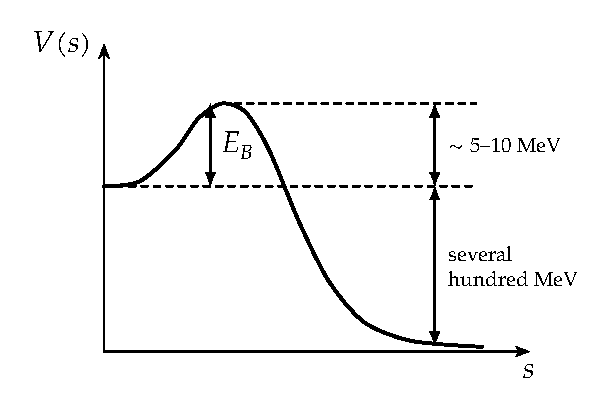
\includegraphics[width=0.75\linewidth]{pictures/1_17}
\par\end{centering}
\centering{}\caption{\label{fig:1_17}液滴裂变势垒的示意图。}
\end{figure}

在裂变的动力学描述中，下一步将是计算动能（即质量参数，它们无疑依赖于形变 \cite{HD71,Gr71}）。既然流体动力学模型在处理小振动时未能给出令人满意的质量参数，我们自然无法指望它在此处能有良好表现。我们将在
12.3.7 节中看到通常如何计算这些物理量。

最终的步骤将是合理的量子化以及对所得 Schrödinger 方程的求解。详细讨论这些问题远远超出了本章的范围。我们在此仅指出，通常由一维势垒穿透的
WKB 公式来计算自发裂变的寿命 \cite{Wi64}。该公式的核心输入要素正是势能$V(s)$的形状，如\ref{fig:1_17}所示。

遗憾的是，液滴模型无论如何都无法定量地描述核裂变，其主要缺陷之一在于：液滴总是裂变为两个质量相等的碎片，而实验中原子核却极频繁地裂变为质量不等的两块碎片（非对称裂变）。裂变势垒是一个由两个巨大数字相减所得的微小数值，这一事实表明核裂变是一个极其微妙的过程，我们很容易理解，单粒子运动中的量子效应（如壳效应，见
2.9 节）会对它产生决定性的深刻影响。

\section{转动液滴的稳定性\label{sec:=008F6C=0052A8=006DB2=006EF4=007684=007A33=005B9A=006027}}

我们在 1.5 节中已经看到，在液滴围绕球形表面的振动中存在着类似于转动的运动。然而，为了将转动从振动中解耦出来，我们要求存在稳定的有限形变，而这只能由量子力学的壳效应来解释。事实上，实验中观测到的转动谱充分证实了这一假定的合理性。

重离子碰撞实验使得向原子核注入极大的角动量（高达 $80\sim100\,\hbar$）成为可能。在如此高的激发下，人们预期微观量子效应不再起支配作用，于是人们自然要追问：具有如此高旋转角速度的经典液滴将如何表现？

因此，在本节中我们仅关注一个纯粹的经典问题：一个具有清晰表面、带有电荷且具有一定表面能的不可压缩液滴，在绕空间固定轴转动时将具有怎样的物理行为。我们对表面振动不感兴趣，而是寻求该系统的稳定平衡形状。

我们再次需要对液滴内部的流动结构作出假定，在此我们将假定为刚体转动；即转动惯量由下式给出：
\begin{equation}
\mathcal{J}=\mathcal{J}^{\text{rig}}=\int_{V}r^{2}_{\perp}\rho_{0}\,\mathrm{d}^{3}\boldsymbol{r},\label{eq:1.84}
\end{equation}
其中$r_{\perp}$是体积元$\mathrm{d}^{3}\boldsymbol{r}$距转动轴的垂直距离。正如我们将在
3.4 节中看到的，该假定非常合理，因为人们预期在高角动量极限下原子核的转动惯量将趋近于刚体转动惯量值。

这一问题与天体物理中著名的自引力不可压缩均匀旋转质量体问题非常相似。在天体问题中，吸引力是万有引力，它与 Coulomb 力具有完全相同的数学结构（但符号相反），且表面力被忽略不计。从
Newton 开始，这一问题就被许多著名数学家广泛研究（历史评述见 \cite[第 1 章]{Ch69}）。

所得结果之一是：没有表面张力的自引力液滴在转动角速度$\omega\rightarrow0$时呈球形。当$\omega>0$时，它首先呈现严格的以转动轴为对称轴的扁椭球形状（Maclaurin
形状）。随着$\omega$的增大，它变得越来越扁，直到某一临界角速度$\omega_{I}$。对于大于$\omega_{I}$的$\omega$值，出现了一种新型的稳定形状\footnote{这对应于一个二级相变 \cite{BR76}。}——三轴椭球（Jacobi
形状）——此时液滴绕其最短的主轴转动。该点$\omega_{I}$称为分叉点（bifurcation point），因为当$\omega>\omega_{I}$时，Maclaurin
形状虽然仍是定态极值解，但在某些自由度上已不再是能量极小值 \cite{Ro67}。人们称之为长期不稳定（secularly unstable）。然而，在没有摩擦力的均匀转动系统（陀螺系统）中，它们仍能表现出稳定的运动（普通稳定性，ordinary
stability）\cite{Ly58}。沿着 Jacobi 形状向更高的$\omega$值追踪，将到达进一步的分叉点，演化出新的平衡形状，直至最终液滴破裂瓦解。

Cohen、Plasil 与 Swiatecki \cite{CPS74} 研究了转动核液滴的稳定性问题。他们寻找能量面的驻点解：
\begin{align}
E(\boldsymbol{\alpha}) & =E_{s}(\boldsymbol{\alpha})+E_{C}(\boldsymbol{\alpha})+E_{R}(\boldsymbol{\alpha})\nonumber \\
 & =E_{s}(0)(B_{s}(\boldsymbol{\alpha})+2x\cdot B_{C}(\boldsymbol{\alpha})+yB_{R}(\boldsymbol{\alpha})).\label{eq:1.85}
\end{align}
除了表面能（$E_{s}$）与 Coulomb 能（$E_{C}$）之外 {[}参见式 (1.32) 等{]}，我们现在还计入了在给定角动量$I$下的转动能：
\begin{equation}
E_{R}(\boldsymbol{\alpha})=\frac{\hbar^{2}I^{2}}{2\mathcal{J}(\boldsymbol{\alpha})}=yE_{s}(0)B_{R}(\boldsymbol{\alpha}).\label{eq:1.86}
\end{equation}
零形变下的转动惯量由式 (1.84) 给出：$\mathcal{J}(0)=\frac{2}{5}MR^{2}_{0}$。除了度量
Coulomb 能与表面能相对比例的可裂变度参数$x$之外，现在还出现了新的旋转参数：
\begin{equation}
y=\frac{E_{R}(0)}{E_{s}(0)}=\frac{5}{16\mathrm{\pi}}\frac{\hbar^{2}I^{2}}{\sigma mr^{4}_{0}}\frac{1}{A^{7/3}}\approx2I^{2}A^{-7/3},\label{eq:1.87}
\end{equation}
它度量了转动能与表面能的相对大小。参数$x$和$y$完全由原子核本身的内秉属性以及所感兴趣的角动量决定；其余的计算纯粹是几何学问题。

这些研究 \cite{CPS74} 的结论是：原子核的表现与自引力液滴极为相似。在低角动量（低$y$值）下，原子核呈现绕转动轴轴对称的扁平形状。它们被称为
Hiskes 形状，与严格的扁椭球（Maclaurin 形状）十分相似。它们在达到临界值$y_{I}$（对应于 Jacobi 点）之前保持稳定。$y_{I}$的数值依赖于$x$。对于极重核$x>0.81$，当$y>y_{I}$时系统直接发生裂变。对于其余的原子核，则演化出一种新型的稳定形状。这些形状被称为
Beringer-Knox 形状 \cite{BK61}，与 Jacobi 形状相似。在极高角动量下，这些形状绕垂直于原对称轴的轴变得近乎轴对称，并最终对裂变变得不稳定（$y_{II}$）。

上述计算涉及大量的形变参数。如果将形状限制为严格的三轴椭球，其半轴$a_{1},a_{2},a_{3}$可由两个参数$\beta$和$\gamma$所表征\footnote{我们此前在描述核表面的微小四极形变时已经使用了 Hill-Wheeler 坐标$\beta$与$\gamma$ {[}式 (1.13){]}。在此我们通过半轴将核表面定义为严格的椭球。这正是
Hill 和 Wheeler \cite{HW53} 的原始定义。它仅在小$\beta$值极限下才与式 (1.7) 一致。}：
\begin{equation}
a_{\kappa}=R_{0}\exp\left\{ \sqrt{\frac{5}{4\mathrm{\pi}}}\beta\cos\left(\gamma-\frac{2\mathrm{\pi}}{3}\kappa\right)\right\} \quad(\kappa=1,2,3).\label{eq:1.88}
\end{equation}
该定义保证了体积的守恒性。

\begin{figure}[H]
\begin{centering}
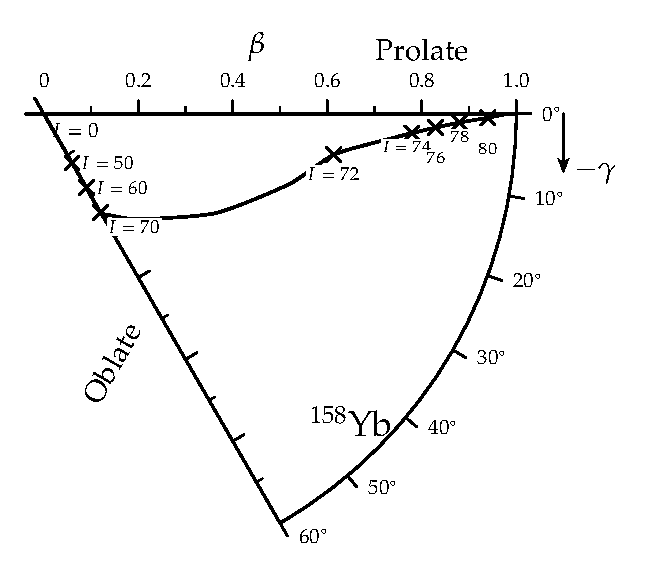
\includegraphics[width=0.75\linewidth]{pictures/1_18}
\par\end{centering}
\centering{}\caption{\label{fig:1_18}作为角动量$I$函数的转动液滴平衡形状（以$\beta$和$\gamma$表示）。由于 1
轴为转动轴，与通常三个轴完全等价的情形相反，此处需要负的$\gamma$值。核素$^{158}\text{Yb}$的参数值为$x=0.618$（引自
\cite{ALL76}）。}
\end{figure}

计算这些椭球的刚体转动惯量、表面能与 Coulomb 能\footnote{参见例如 \cite{Ca61,CM63}。}作为$\beta$和$\gamma$的函数相对较为简便，并可进而寻找对应于每个$I$值的能量面极小值。将这些稳定平衡形状连接起来，便在$\beta$-$\gamma$平面上得到一条轨迹，如\ref{fig:1_18}所示。

对于每个给定的$I$，我们都拥有一张能量曲面并研究其局域极小值。正如在$I=0$的情形下一样（1.6 节），除了极小值之外，还存在着一个带有鞍点的裂变能谷。由于离心力的作用，势垒高度随着角动量的增加而减小；当势垒彻底消失时，该形状族对裂变变得完全不稳定。作为一个例子，我们考虑原子核$^{127}\text{La}$
\cite{CPS74}。在零角动量$I=0$时，其液滴模型裂变势垒高达$40.0\,\text{MeV}$。其 Jacobi
点（$y_{I}$）对应于$I=67.8\,\hbar$。在此角动量下，其激发能达到$44.31\,\text{MeV}$ {[}$E_{s}(0)=49.5\,\text{MeV}${]}，而裂变势垒高度骤降至仅剩$7.8\,\text{MeV}$。

从这一考量中可以清晰地看出：任何原子核都无法承受超过某一极限角动量的旋转，否则它将对裂变发生失稳。在\ref{fig:1_19}中，展示了处于$\beta$稳定线
{[}由$N=A/2+0.2\cdot A^{2}/(200+A)$所近似{]} 上的原子核裂变势垒完全消失时的角动量$I_{II}$随质量数$A$的变化关系。轻核由于自身尺寸过小而无法承载过多的角动量单位；重核由于
Coulomb 能的排斥而稳定性降低；位于$A\simeq130$附近的原子核可以达到最高的旋转角动量（约$100\,\hbar$）。重离子碰撞实验
\cite{BES76} 的结果与液滴模型给出的这些极限值表现出良好的一致性。

\begin{figure}[H]
\begin{centering}
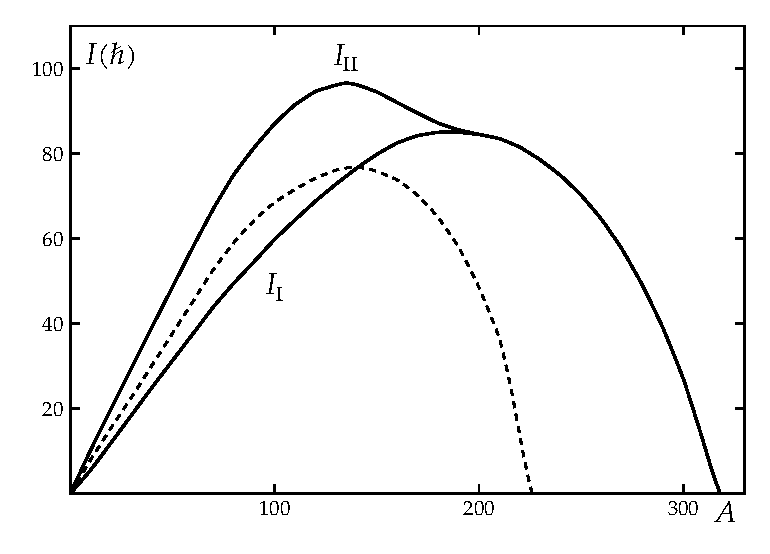
\includegraphics[width=0.75\linewidth]{pictures/1_19}
\par\end{centering}
\centering{}\caption{\label{fig:1_19}处于$\beta$稳定线上的质量数为$A$的原子核所能承受的最大角动量$I_{II}$以及临界角动量$I_{I}$（Jacobi
分叉点）。虚线对应于裂变势垒高度为$8\,\text{MeV}$的曲线，这一势垒高度保证了对裂变具有合理的寿命（引自 \cite{CPS74}）。}
\end{figure}




\chapter{壳模型\label{chap:=0058F3=006A21=00578B}}

\section{引言与普遍考虑\label{sec:=005F15=008A00=004E0E=00666E=00904D=008003=008651}}

在上一章中我们探讨了原子核的宏观整体性质，即全核或绝大部分核子协同参与的静态或动态集体行为。在这一章中，我们将讨论原子核完全不同的另一个重要物理层面：大量实验事实表明，核内的核子在很大程度上可以被视为在几乎未受扰动的单粒子轨道上独立运动的粒子。

正如我们在第 1 章开头指出的，独立粒子图像之所以在原子核这样强相互作用体系中成立，主要归因于 Pauli 不相容原理和量子力学测不准原理的深刻制约。现代核物理已经确立，现实核子-核子力在芯部（$c\simeq0.4\,\text{fm}$）处具有极强的硬芯排斥
\cite{Vi78}。因此，密堆积体积 $V_{c}$ 与原子核实际体积 $V$ 之比仅为 \cite{BM69}：

\begin{equation}
\frac{V_{c}}{V}=\left(\frac{c}{2r_{0}}\right)^{3}\simeq\frac{1}{100}\label{eq:packing_fraction}
\end{equation}

这意味着平均而言核子之间的距离相对较远，核子通常仅“感受”到核力吸引长程尾部。短程强排斥所诱发的剧烈硬碰撞由于 Pauli 原理对末态相空间的强烈冻结而极其罕见。由核散射实验估计的核内核子平均自由程至少与原子核自身线度相当
\cite{BM69,KK68}，这为核内独立粒子运动提供了最初步的坚实实验支撑。既然核子近似独立运动，这些单粒子运动必然受控于由所有其他核子共同产生的平均单体势阱中。

\section{壳效应的实验证据\label{sec:=0058F3=006548=005E94=007684=005B9E=009A8C=008BC1=00636E}}

核平均势的存在直接导致了类似于原子物理中电子壳层的特征能级聚集现象。实验上发现的核物理幻数（Magic numbers）：

\[
2,\;8,\;20,\;28,\;50,\;82,\;126
\]

构成了建立核壳模型最强有力的实验基石。在这些中子数或质子数处，原子核表现出异常强大的结合与极高的稳定性：
\begin{itemize}
\item 单粒子分离能：将最弱束缚核子从核中移走所需的能量定义为分离能 $S_{n}$ 或 $S_{p}$。图 2.1 表明，通常核的分离能约为
8 MeV，但在幻数处出现极为陡峭的骤降，双满壳核的分离能显著偏高，这一突变特征与原子稀有气体的电离能跃变完全类似；
\end{itemize}
\begin{figure}[H]
\begin{centering}
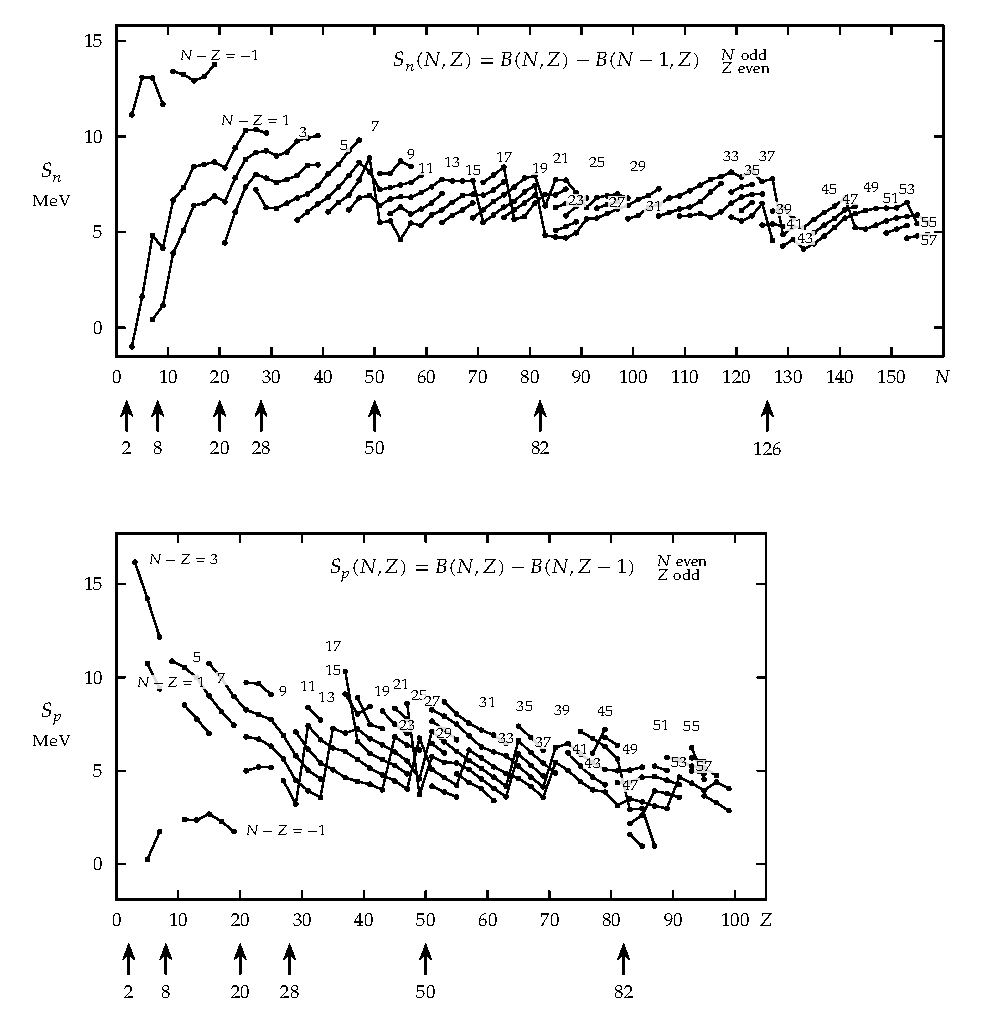
\includegraphics[width=0.75\textwidth]{pictures/2_1}
\par\end{centering}
\caption{\label{fig:2_1}图 2.1 中子与质子分离能分别作为中子数和质子数的函数（引自 {[}Ir 72{]}）。}
\end{figure}

\begin{itemize}
\item 质量与结合能偏差：实验核质量对 Bethe-Weizsäcker 半经验平滑质量公式的偏离（图 2.2）在幻数处呈现出极其显著的深下凹尖峰，表明幻数核具有异常强大的额外束缚能；
\end{itemize}
\begin{figure}[H]
\begin{centering}
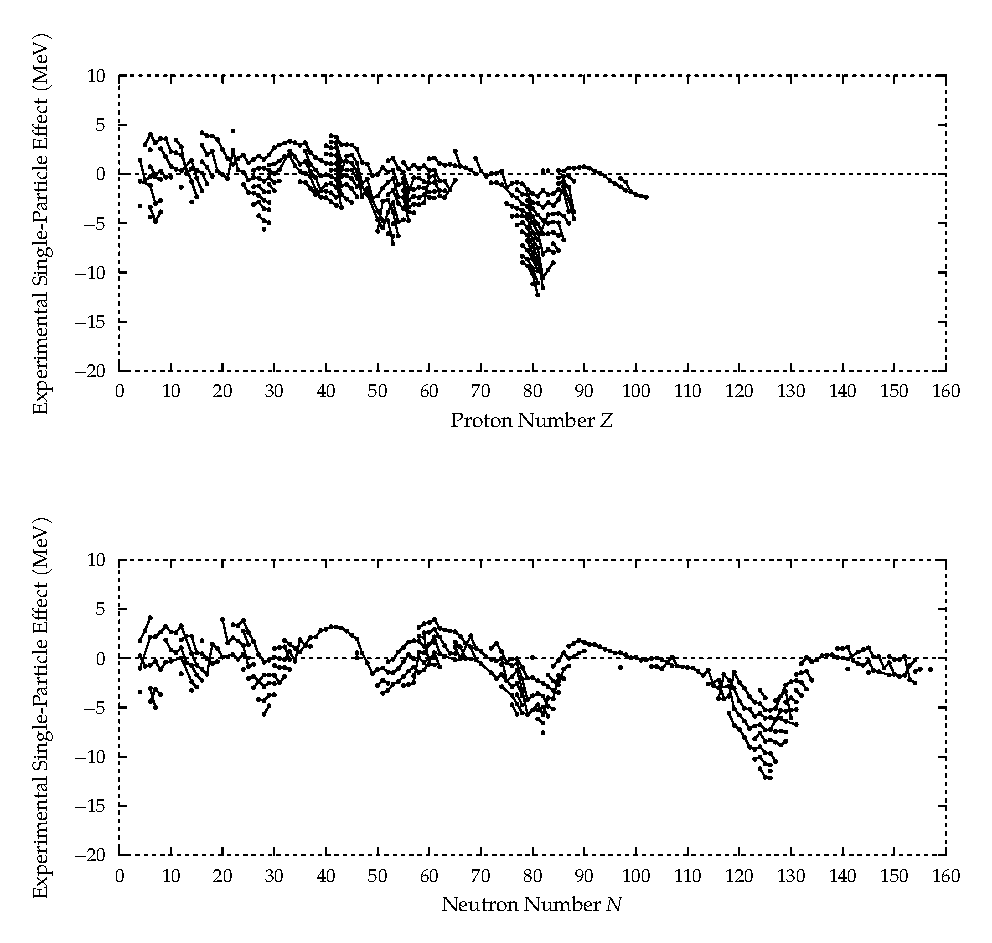
\includegraphics[width=0.75\textwidth]{pictures/2_2}
\par\end{centering}
\caption{\label{fig:2_2}图 2.2 实验核质量对平均平滑值的偏离作为中子数和质子数的函数（引自 {[}MS 66{]}）。}
\end{figure}

\begin{itemize}
\item 第一激发态能量与集体性：偶偶核的第一激发态 $2^{+}$ 能量在幻数闭壳处急剧升高（图 1.7），表明闭壳核对外场扰动具有极高的刚性，难以发生集体激发。
\end{itemize}

\section{原子核的平均势\label{sec:=00539F=005B50=006838=007684=005E73=005747=0052BF}}

在原子中，电子围绕带正电的原子核运动，天然存在一个外部提供的中心 Coulomb 场。而原子核内不存在任何外部中心场，其平均单体势阱是所有核子通过双体相互作用自洽形成的。在中心区域，核子受力均匀对称，净受力为零：

\begin{equation}
\left(\frac{\partial V}{\partial r}\right)_{r=0}=0\label{eq:pot_center_slope}
\end{equation}

随着离开核中心向核表面（$r=R_{0}$）过渡，束缚势阱逐渐变浅，$(\partial V/\partial r)_{r<R_{0}}>0$；在核外因强相互作用为短程力而迅速趋于零：$V(r)\to0$（$r\gg R_{0}$）。能够优美满足这些物理边界条件并与核电荷分布高度一致的唯象势是
Woods-Saxon 势 \cite{WS54}：

\begin{equation}
V_{\text{WS}}(r)=-V_{0}\left[1+\exp\left(\frac{r-R_{0}}{a}\right)\right]^{-1}\label{eq:woods_saxon_spherical}
\end{equation}

\begin{figure}[H]
\begin{centering}
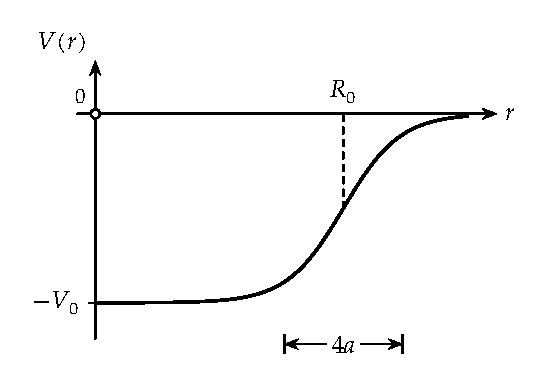
\includegraphics[width=0.75\textwidth]{pictures/2_3}
\par\end{centering}
\caption{\label{fig:2_3}图 2.3 Woods-Saxon 势的形式。}
\end{figure}

典型参数为势阱深度 $V_{0}\simeq50\,\text{MeV}$，核半径 $R_{0}=r_{0}A^{1/3}$（$r_{0}\simeq1.25\,\text{fm}$），表面弥散厚度参数
$a\simeq0.65\,\text{fm}$。为了解析讨论，物理上常采用两种极端势阱近似：
\begin{enumerate}
\item 各向同性谐振子势：$V(r)=-V_{0}+\frac{1}{2}m\omega^{2}_{0}r^{2}$；
\item 球方势阱：当 $r\leqslant R_{0}$ 时 $V(r)=-V_{0}$，当 $r>R_{0}$ 时 $V(r)=0$（或考虑无穷深球方势阱）。
\end{enumerate}
对于三维球形谐振子，能级为等间距能级：

\begin{equation}
\varepsilon_{N}=\hbar\omega_{0}\left(N+\frac{3}{2}\right)-V_{0},\quad N=2(n-1)+l\label{eq:ho_spectrum_spherical}
\end{equation}

其中主量子数 $N=0,1,2,\dots$，径向量子数 $n=1,2,\dots$，轨道角动量 $l=0,1,\dots,N$
与 $N$ 具有相同的奇偶性（同一振子壳层只包含相同宇称态）。考虑自旋后，每个主振子壳层的简并度为：

\begin{equation}
D(N)=(N+1)(N+2)\label{eq:ho_degeneracy}
\end{equation}

谐振子频率 $\hbar\omega_{0}$ 可由核电荷均方半径与核饱和密度确定 \cite{Mo57}：

\begin{equation}
\hbar\omega_{0}\simeq\frac{5}{4}\left(\frac{3}{2}\right)^{1/3}\frac{\hbar^{2}}{mr^{2}_{0}}A^{-1/3}\simeq41\cdot A^{-1/3}\,\text{[MeV]}\label{eq:period_of_shell}
\end{equation}

振子特征长度为 $b=\sqrt{\hbar/(m\omega_{0})}\simeq1.01\cdot A^{1/6}\,\text{[fm]}$。谐振子势填满主壳层的累积核子数为：2,
8, 20, 40, 70, 112, 168。在更真实的方势阱或 Woods-Saxon 势中，由于势阱边界比谐振子势更陡峭，高
$l$ 轨道的能量显著降低，从而消除了谐振子势中的偶然简并，给出能级序列：$1s,1p,1d,2s,1f,2p,1g,\dots$，对应的壳闭合幻数为
2, 8, 20, 34, 40, 58, 92, 138。显然，无论是谐振子势还是球方势阱，都只能解释前三个幻数（2, 8, 20），而完全无法给出重核区正确的实验幻数
28, 50, 82, 126。

\begin{figure}[H]
\begin{centering}
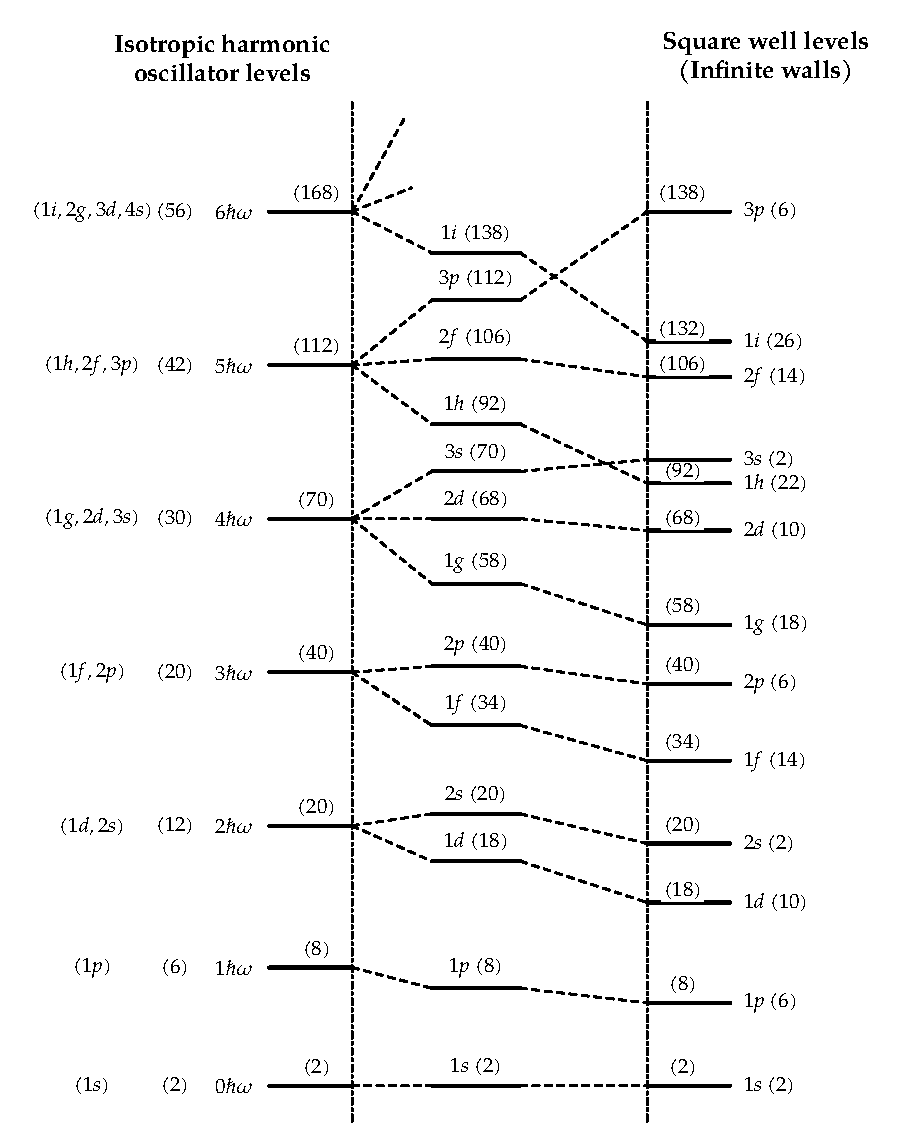
\includegraphics[width=0.75\textwidth]{pictures/2_4}
\par\end{centering}
\caption{\label{fig:2_4}图 2.4 各向同性谐振子（左）与无限深球方势阱（右）的单粒子能级方案（引自 {[}MJ 55{]}）。}
\end{figure}


\section{自旋-轨道耦合\label{sec:=0081EA=0065CB-=008F68=009053=008026=005408}}

1949 年，Mayer \cite{Ma49} 与 Haxel、Jensen、Suess \cite{HJS49} 独立提出，解决这一重大难题的关键在于核单粒子势中存在强大的自旋-轨道相互作用：

\begin{equation}
V_{ls}(\boldsymbol{r})=V_{ls}(r)\boldsymbol{l}\cdot\boldsymbol{s}=\kappa\frac{1}{r}\frac{\mathrm{d}V(r)}{\mathrm{d}r}\,\boldsymbol{l}\cdot\boldsymbol{s}\label{eq:spin_orbit_potential}
\end{equation}

与原子中由相对论 Thomas 进动引起的微弱自旋-轨道耦合不同，核物理中的自旋-轨道力强度不仅比原子大近 30 倍，而且符号相反（$\kappa<0$）。核子的总单粒子角动量为
$\boldsymbol{j}=\boldsymbol{l}+\boldsymbol{s}$，由 $\boldsymbol{l}\cdot\boldsymbol{s}=\frac{1}{2}(\boldsymbol{j}^{2}-\boldsymbol{l}^{2}-\boldsymbol{s}^{2})$
可得算符本征值为：

\begin{equation}
\langle\boldsymbol{l}\cdot\boldsymbol{s}\rangle=\begin{cases}
\frac{1}{2}l, & \text{对于 }j=l+\frac{1}{2}\\
-\frac{1}{2}(l+1), & \text{对于 }j=l-\frac{1}{2}
\end{cases}\label{eq:ls_eigenvalues}
\end{equation}

由此导致的同一 $l$ 轨道的能级分裂量为：

\begin{equation}
\Delta\varepsilon_{ls}=\varepsilon_{j=l-1/2}-\varepsilon_{j=l+1/2}=\left(l+\frac{1}{2}\right)\langle V_{ls}\rangle\label{eq:ls_splitting}
\end{equation}

由于 $V_{ls}(r)$ 为强吸引作用，平行耦合的轨道（$j=l+1/2$）能量大幅度下移，而反平行轨道（$j=l-1/2$）能量上移。分裂量正比于
$2l+1$，随轨道角动量 $l$ 急剧增大！在每个主要高能壳层中，具有最高角动量的支能级：
\begin{itemize}
\item $1f_{7/2}$（来自 $N=3$ 壳）被强力压低，在 20 之后容纳 8 个核子，形成幻数 $\mathbf{28}$；
\item $1g_{9/2}$（来自 $N=4$ 壳）侵入下一壳层，在 40 之后容纳 10 个核子，形成幻数 $\mathbf{50}$；
\item $1h_{11/2}$（来自 $N=5$ 壳）侵入形成幻数 $\mathbf{82}$；
\item $1i_{13/2}$（来自 $N=6$ 壳）侵入形成幻数 $\mathbf{126}$。
\end{itemize}
这些被强自旋-轨道耦合压入低主振子壳层的高角动量轨道被称为侵入态（Intruder states）。它们与其所在壳层中的其他轨道具有相反的宇称，因而在单核子衰变中受到宇称选择定则的强力保护。由此，包含强自旋-轨道相互作用的球形单粒子壳模型彻底、自然地解释了全核素区的全部幻数（图
2.5）！

\begin{figure}[H]
\begin{centering}
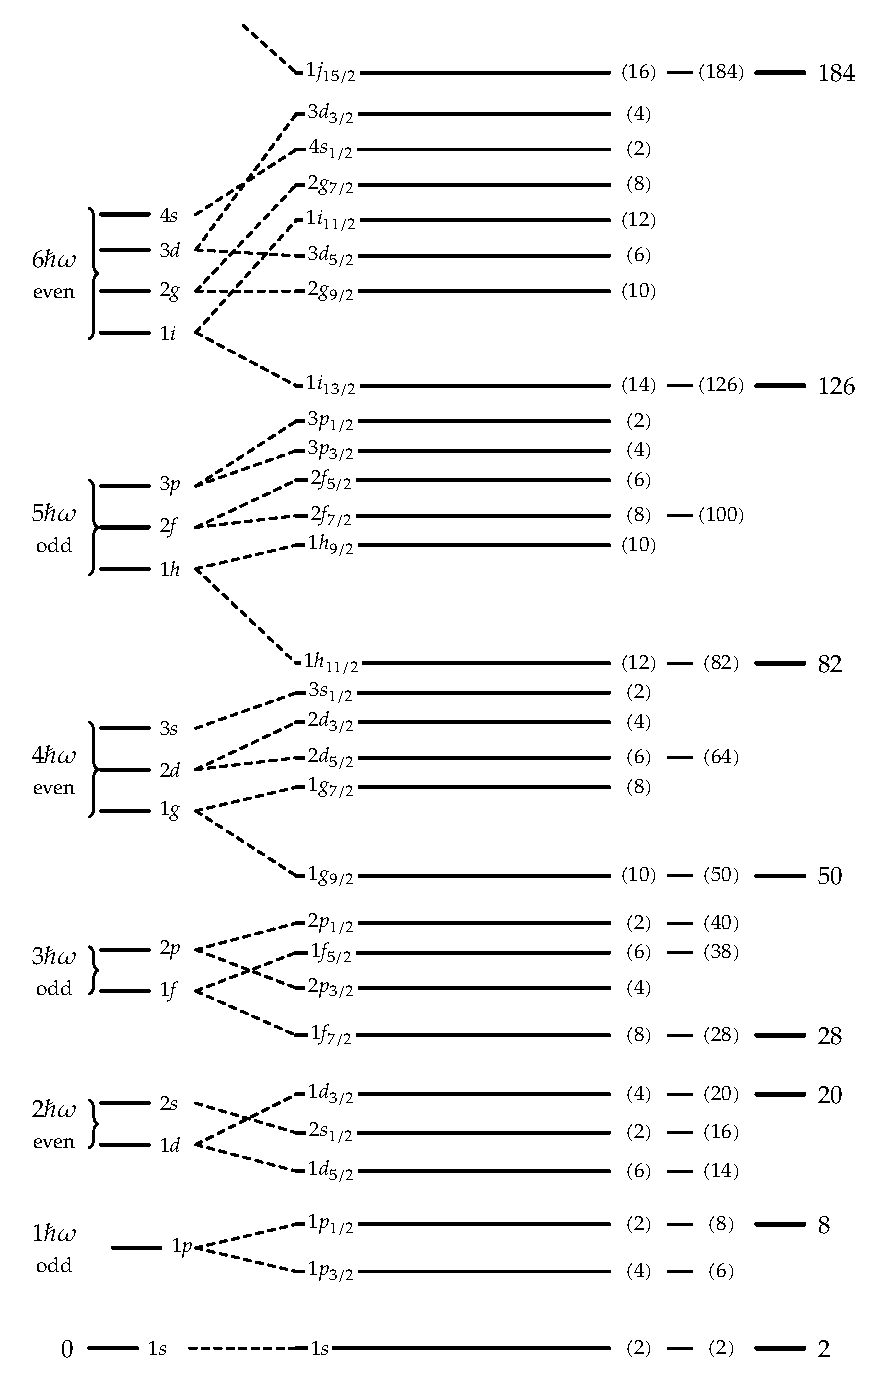
\includegraphics[width=0.75\textwidth]{pictures/2_5}
\par\end{centering}
\caption{\label{fig:2_5}图 2.5 包含自旋-轨道耦合项的壳模型核能级示意图（引自 {[}MJ 55{]}）。}
\end{figure}


\section{多体问题的壳模型方法\label{sec:=00591A=004F53=0095EE=009898=007684=0058F3=006A21=00578B=0065B9=006CD5}}

严格的原子核微观理论建立在非相对论量子多体问题之上，其总微观 Hamilton 量包含核子动能与两体相互作用：

\begin{equation}
H=\sum^{A}_{i=1}t_{i}+\frac{1}{2}\sum^{A}_{i\neq j}v(i,j)\label{eq:full_microscopic_H}
\end{equation}

其中 $i=(\boldsymbol{r}_{i},\boldsymbol{s}_{i},\boldsymbol{t}_{i})$
表示单个核子的全部空间、自旋与同位旋坐标。壳模型方法的核心思想是在总 Hamilton 量中引入一个平均单粒子势场 $U(i)$，并将全
Hamilton 量精确分解为无相互作用的独立粒子单体 Hamilton 量 $H_{0}$ 与剩余相互作用（Residual interaction）$V_{\text{res}}$：

\begin{equation}
H=H_{0}+V_{\text{res}}\label{eq:H_split_H0_Vres}
\end{equation}

其中：

\begin{align}
H_{0} & =\sum^{A}_{i=1}h(i)=\sum^{A}_{i=1}\left[t_{i}+U(i)\right]\nonumber \\
V_{\text{res}} & =\frac{1}{2}\sum^{A}_{i\neq j}v(i,j)-\sum^{A}_{i=1}U(i)\label{eq:V_residual_def}
\end{align}

求解单粒子薛定谔方程：

\begin{equation}
h(i)\phi_{k}(i)=\varepsilon_{k}\phi_{k}(i)\label{eq:single_particle_schrodinger}
\end{equation}

本征态 $\phi_{k}$ 构成二次量子化表象（附录 C）的正交归一基底。设 $a^{\dagger}_{k}$ 与 $a_{k}$
分别为轨道 $k$ 上的费米子产生与湮灭算符，则独立粒子 Hamilton 量可写为：

\begin{equation}
H_{0}=\sum_{k}\varepsilon_{k}a^{\dagger}_{k}a_{k}\label{eq:H0_second_quantized}
\end{equation}

对于双满壳闭壳核，核子从最低轨道一直填到 Fermi 能级 $\varepsilon_{F}$，体系基态由单一 Slater 行列式给出：

\begin{equation}
|\Phi_{0}\rangle=\prod_{i\leqslant\varepsilon_{F}}a^{\dagger}_{i}|-\rangle\label{eq:slater_ground_state}
\end{equation}

\begin{figure}[H]
\begin{centering}
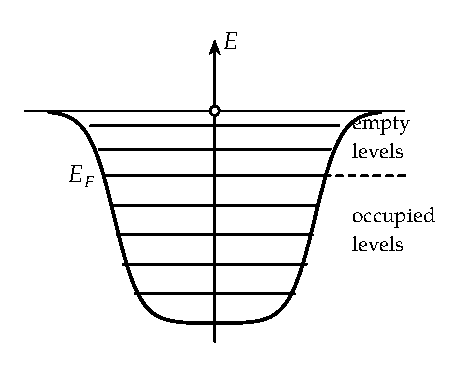
\includegraphics[width=0.75\textwidth]{pictures/2_6}
\par\end{centering}
\caption{\label{fig:2_6}图 2.6 壳模型势阱与费米能级示意图。}
\end{figure}

对于中子过剩核，由于质子感受到额外的 Coulomb 排斥能，其势能曲面整体上移；同时核对称能使质子感受到的核势部分比中子势更深，从而使中子与质子的
Fermi 面得以保持平衡（图 2.7）。

\begin{figure}[H]
\begin{centering}
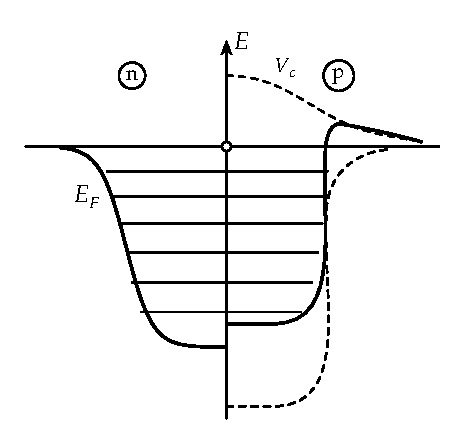
\includegraphics[width=0.75\textwidth]{pictures/2_7}
\par\end{centering}
\caption{\label{fig:2_7}图 2.7 中子过剩核中中子与质子壳模型势的比较（虚线对应更深的质子核势部分）。}
\end{figure}

在 Fermi 气体图像下，体系最简单的激发态是将 Fermi 海中的一个核子 $i$（$\varepsilon_{i}\leqslant\varepsilon_{F}$）激发到空轨道
$m$（$\varepsilon_{m}>\varepsilon_{F}$）上，形成粒子-空穴激发态（$1p-1h$ 态）：

\begin{equation}
|\Phi_{mi}\rangle=a^{\dagger}_{m}a_{i}|\Phi_{0}\rangle,\quad\Delta E_{mi}=\varepsilon_{m}-\varepsilon_{i}\label{eq:ph_excitation}
\end{equation}

\begin{figure}[H]
\begin{centering}
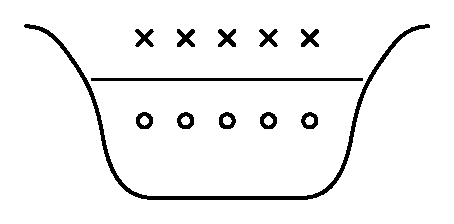
\includegraphics[width=0.75\textwidth]{pictures/2_8}
\par\end{centering}
\caption{\label{fig:2_8}图 2.8 典型的五粒子（叉号）五空穴（空心圆）激发态示意图。}
\end{figure}

极其便利的工具是定义准粒子（Quasiparticles）：

\begin{equation}
\alpha^{\dagger}_{m}=a^{\dagger}_{m}\;(\varepsilon_{m}>\varepsilon_{F}),\quad\alpha^{\dagger}_{i}=a_{i}\;(\varepsilon_{i}\leqslant\varepsilon_{F})\label{eq:quasiparticle_particle_hole}
\end{equation}

使得基态成为准粒子真空态：$\alpha_{k}|\Phi_{0}\rangle=0$。真实的核基态由于剩余相互作用 $V_{\text{res}}$
的存在，包含着虚粒子-空穴激发的相关混杂：

\begin{equation}
|\Psi\rangle=c_{0}|\Phi_{0}\rangle+\sum_{mi}c_{mi}a^{\dagger}_{m}a_{i}|\Phi_{0}\rangle+\frac{1}{4}\sum_{mnij}c_{mnij}a^{\dagger}_{m}a^{\dagger}_{n}a_{j}a_{i}|\Phi_{0}\rangle+\dots\label{eq:ground_state_correlation_expansion}
\end{equation}

在良好的平均场势阱下，展开系数满足 $c_{0}\approx1$，高阶关联较小。如何在微观上自洽决定最优平均势 $U(i)$
使得剩余相互作用最小，正是第 5 章 Hartree-Fock 理论的核心议题。

\section{对称性\label{sec:=005BF9=0079F0=006027}}

\subsection{平移对称性}

真实的原子核 Hamilton 量在全空间中具有严格的平移不变性。然而在唯象壳模型中，为了定义单粒子势场，我们人为地将平均势的中心固定在空间原点，这必然破坏了平移对称性。这种对称性破缺带来的最直接后果是：体系的激发能谱中混入了多余的自由度，产生所谓的赝态或赝模（Spurious
states / Spurious modes）。

由于一个包含 $A$ 个核子的体系只有 $3A-3$ 个内秉自由度，壳模型的 $3A$ 个坐标中包含了核质心整体在势阱中的振荡运动。在谐振子势中，总
Hamilton 量可以精确分离为质心部分与相对运动部分：

\begin{equation}
H=H_{\text{c.m.}}+H_{\text{rel}}=\left(\frac{\boldsymbol{P}^{2}}{2mA}+\frac{1}{2}mA\omega^{2}_{0}\boldsymbol{R}^{2}\right)+H_{\text{rel}}\label{eq:trans_cm_separation}
\end{equation}

其中 $\boldsymbol{R}=\frac{1}{A}\sum_{i}\boldsymbol{r}_{i}$，$\boldsymbol{P}=\sum_{i}\boldsymbol{p}_{i}$。因此质心零点能为
$\frac{3}{2}\hbar\omega_{0}$。为了消除赝质心动能带来的误差，通常从总能量中减去质心动能期望值 $\langle\boldsymbol{P}^{2}\rangle/(2mA)$；在第
11 章中我们将系统讨论通过投影算符方法严格消除平移赝态的微观理论。

\subsection{转动对称性与组态混合}

球形壳模型 Hamilton 量 $H_{0}$（包含自旋-轨道耦合项）与总角动量算符 $\boldsymbol{J}^{2}$
及 $J_{z}$ 对易：

\begin{equation}
\boldsymbol{J}=\sum^{A}_{i=1}\boldsymbol{j}_{i},\quad J_{z}=\sum^{A}_{i=1}j_{zi}\label{eq:total_J_def}
\end{equation}

对于双满壳闭壳核，所有单粒子态全部被填满，基态唯一的总角动量本征值严格为 $I=0^{+}$，该结论已被所有双幻核无一例外地实验证实。当闭壳核外只有一个核子（或缺少一个核子形成的单空穴态）时，核基态总角动量自然等于该价核子的单粒子角动量
$I=j$。

当闭壳核外存在两个以上价核子时，同一 $j$ 壳层内不同磁量子数 $m$ 的状态是完全简并的。例如对于同种价核子组态 $(j)^{2}$，根据角动量耦合理论与
Clebsch-Gordan 系数：

\begin{equation}
|IM\rangle=\frac{1}{\sqrt{2}}\sum_{m_{1}m_{2}}C^{IM}_{jm_{1}jm_{2}}|m_{1}m_{2}\rangle\label{eq:cg_two_particle_coupling}
\end{equation}

由于核子是全同费米子，双粒子态满足反对称性 $|m_{2}m_{1}\rangle=-|m_{1}m_{2}\rangle$，结合
Clebsch-Gordan 系数的对称性性质 $C^{IM}_{jm_{2}jm_{1}}=(-1)^{2j-I}C^{IM}_{jm_{1}jm_{2}}$，得到波函数具有因子
$1-(-1)^{2j-I}=1+(-1)^{I}$（因为对半整数 $j$，$2j$ 为奇数）。因此非零的物理态要求总角动量必须为偶数：

\begin{equation}
I=0,2,4,\dots,2j-1\label{eq:even_I_allowed}
\end{equation}

例如对于 $j=3/2$，允许的总角动量仅为 $I=0,2$。为了在这些简并态中确定基态能量并解除简并，必须引入剩余相互作用 $V_{\text{res}}$（式
(2.35)）并在模型组态空间中进行对角化。在真实的核中，配对相互作用使得 $I=0$ 态的能量显著降低，从而在理论上保证了所有偶偶核基态自旋恒为
$0^{+}$。

对于远离闭壳的核，单组态壳模型常常失效，必须考虑组态混合（Configuration mixing）：即真实的核本征态是不同粒子-空穴组态和不同单粒子轨道
Slater 行列式的相干叠加：

\begin{equation}
|\Psi_{I}\rangle=\sum_{\alpha}c_{\alpha}|\Phi_{\alpha}(I)\rangle\label{eq:config_mixing_wavefunction}
\end{equation}

组态混合不仅解除了开壳层能级的简并，而且是微观核结构中产生集体相干性与核形变的核心机制。

\subsection{同位旋}

核力强烈的电荷无关性（Charge independence，见第 4 章）表明，除微弱的电磁相互作用外，质子和中子在强核力作用下表现出高度的一致性。Heisenberg
\cite{He32} 与 Wigner \cite{Wi37} 由此引入了同位旋（Isotopic spin / Isospin）概念，将质子与中子视为同一种粒子——核子（Nucleon）的两个不同内秉荷电状态。

单个核子的同位旋算符由 Pauli 矩阵表示：$\boldsymbol{t}=\frac{1}{2}\boldsymbol{\tau}$，其基矢为：

\begin{equation}
|p\rangle=\begin{pmatrix}1\\
0
\end{pmatrix},\quad|n\rangle=\begin{pmatrix}0\\
1
\end{pmatrix}\label{eq:isospin_spinors}
\end{equation}

在核物理的传统约定中，$t_{3}$ 的本征值为：

\begin{equation}
t_{3}|n\rangle=\frac{1}{2}|n\rangle,\quad t_{3}|p\rangle=-\frac{1}{2}|p\rangle\label{eq:isospin_t3_eigenvals}
\end{equation}

升降算符 $t_{\pm}=t_{1}\pm\mathrm{i}t_{2}$ 实现质子与中子状态的相互跃迁：$t_{-}|n\rangle=|p\rangle$，$t_{+}|p\rangle=|n\rangle$。对于包含
$A$ 个核子的体系，总同位旋矢量算符定义为：

\begin{equation}
\boldsymbol{T}=\sum^{A}_{i=1}\boldsymbol{t}_{i},\quad T_{3}=\sum^{A}_{i=1}t_{3i}=\frac{1}{2}(N-Z)\label{eq:total_isospin_def}
\end{equation}

若忽略 Coulomb 力，总 Hamilton 量与 $\boldsymbol{T}^{2}$ 和 $T_{3}$ 对易，体系的每个定态都具有良好的总同位旋量子数
$T$（满足 $T\geqslant|T_{3}|$）。例如对于质量数 $A=10$ 的同量异位素三胞胎 $\ce{^{10}Be}$（$T_{3}=1$）、$\ce{^{10}B}$（$T_{3}=0$）与
$\ce{^{10}C}$（$T_{3}=-1$），存在严格对应的同位旋三重态（$T=1$，图 2.9）；此外 $\ce{^{10}B}$
独有 $T=0$ 的单态。

\begin{figure}[H]
\begin{centering}
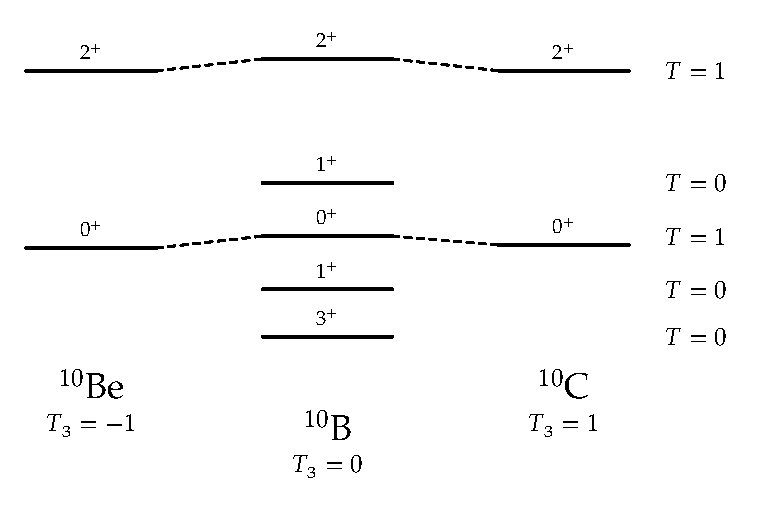
\includegraphics[width=0.75\textwidth]{pictures/2_9}
\par\end{centering}
\caption{\label{fig:2_9}图 2.9 同量异位素激发谱中的同位旋三重态与单态（引自 {[}MJ 55{]}）。}
\end{figure}

由同位旋上升算符 $T_{+}$ 作用在满壳组态上为零可知，所有占据质子能级同时被中子占据的壳模型态必有 $T=T_{3}=(N-Z)/2$，基态组态如图
2.10 所示。

\begin{figure}[H]
\begin{centering}
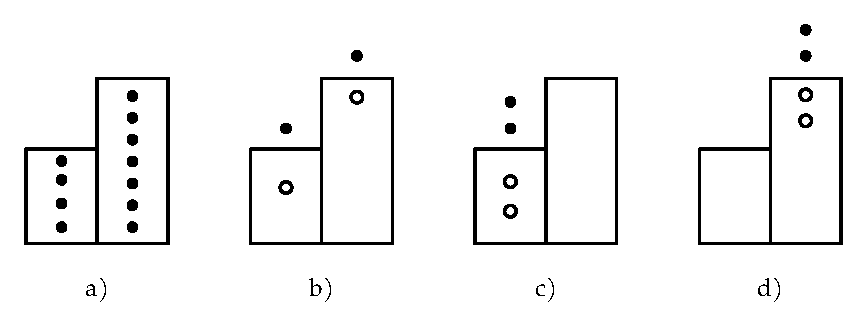
\includegraphics[width=0.75\textwidth]{pictures/2_10}
\par\end{centering}
\caption{\label{fig:2_10}图 2.10 壳模型组态与同位旋示意图。}
\end{figure}

在重核中，虽然质子间巨大的 Coulomb 排斥能破坏了严格的同位旋守恒，但由于大量过剩中子形成了强同位旋矢量单粒子势垒（Symmetry
potential），阻碍了不同同位旋组态的混杂，使得重核低激发态仍然保持着高度纯净的同位旋，并在核反应中观察到了极其清晰锐利的同位旋类似态（Isobaric
Analogue States, IAS）。

\section{与实验对比\label{sec:=004E0E=005B9E=009A8C=005BF9=006BD4}}

\subsection{单粒子（空穴）态的实验证据}

单粒子壳模型最直接的实验检验是在双闭壳核附近的单核子转移反应与敲出反应：
\begin{itemize}
\item 条带反应与单核子拾取：如 $(d,p)$、$(p,d)$、$(d,t)$ 反应，通过测量转移出射粒子的角分布和截面，能够直接提取残核能级的轨道角动量
$l$ 与光谱学因子（Spectroscopic factor）$S_{j}$；
\end{itemize}
\begin{figure}[H]
\begin{centering}
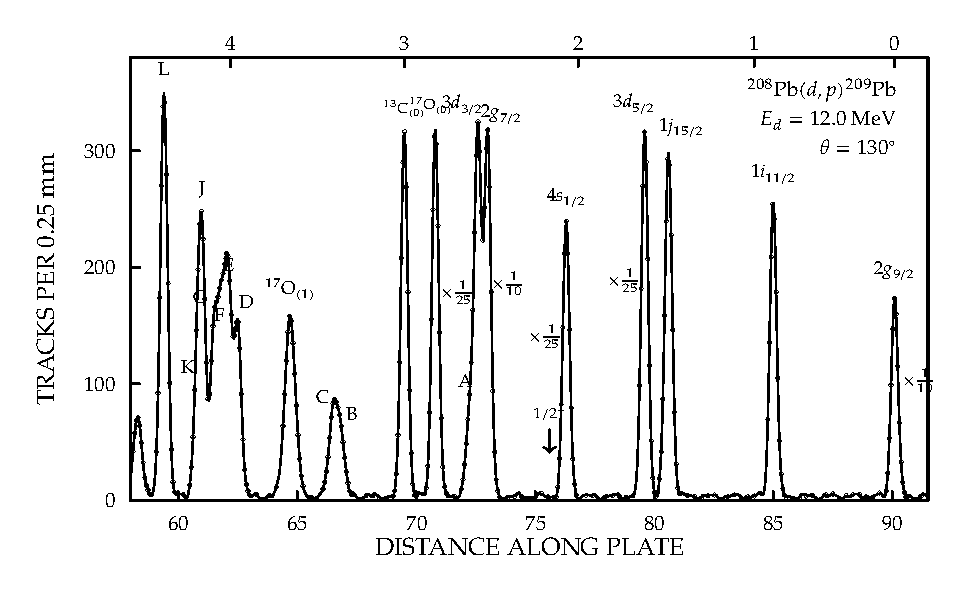
\includegraphics[width=0.75\textwidth]{pictures/2_14}
\par\end{centering}
\caption{\label{fig:2_14}图 2.14 来自 \$\textasciicircum\{208\}}
\end{figure}

\begin{itemize}
\item 准自由散射敲出反应：高能 $(p,2p)$ 与 $(e,e'p)$ 反应能够直接测量原子核深层束缚轨道的单粒子能谱和动量分布（图
2.11 与图 2.13）。
\end{itemize}
\begin{figure}[H]
\begin{centering}
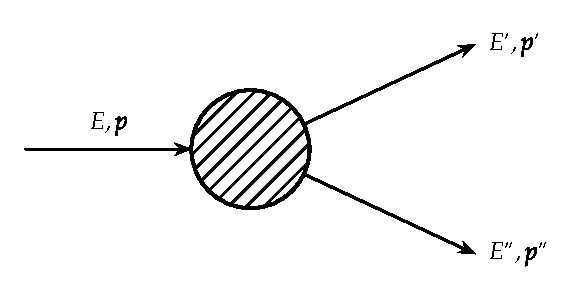
\includegraphics[width=0.75\textwidth]{pictures/2_11}
\par\end{centering}
\caption{\label{fig:2_11}图 2.11 准自由敲出反应 \$(p,2p)\$ 的示意图。}
\end{figure}

在壳模型图像下，被打出核子的束缚能由能量守恒给出：$E_{B}=E-E'-E''$（图 2.12）。

\begin{figure}[H]
\begin{centering}
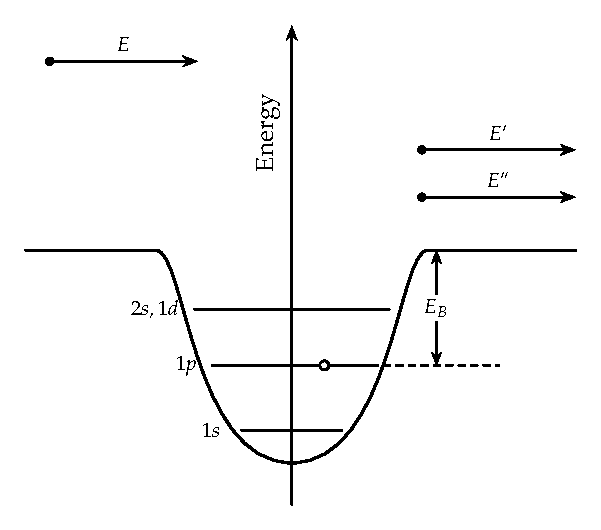
\includegraphics[width=0.75\textwidth]{pictures/2_12}
\par\end{centering}
\caption{\label{fig:2_12}图 2.12 壳模型框架下的 \$(p,2p)\$ 反应过程示意图。}
\end{figure}

\begin{figure}[H]
\begin{centering}
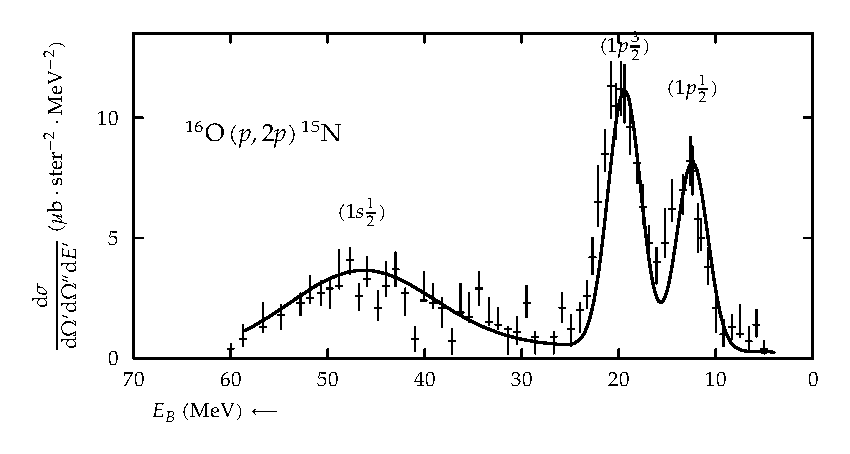
\includegraphics[width=0.75\textwidth]{pictures/2_13}
\par\end{centering}
\caption{\label{fig:2_13}图 2.13 实验测量的 \$\textasciicircum\{16\}}
\end{figure}

图 2.15 给出了双幻核 $\ce{^{208}Pb}$ 邻近奇核（$\ce{^{209}Pb},\ce{^{207}Pb},\ce{^{209}Bi},\ce{^{207}Tl}$）测得的单粒子与单空穴能级同理论
Woods-Saxon 势计算值的对比。实验结果不仅证实了高 $j$ 侵入轨道的存在，而且光谱学因子 $S_{j}\approx1$，说明双闭壳核附近的低激发态确实具有极其纯粹的单粒子特征。远离闭壳时，单粒子强度发生明显的碎裂（Fragmentation），表明单粒子自由度与集体振动（声子）之间存在强烈的粒子-振动耦合（Particle-vibration
coupling）。

\begin{figure}[H]
\begin{centering}
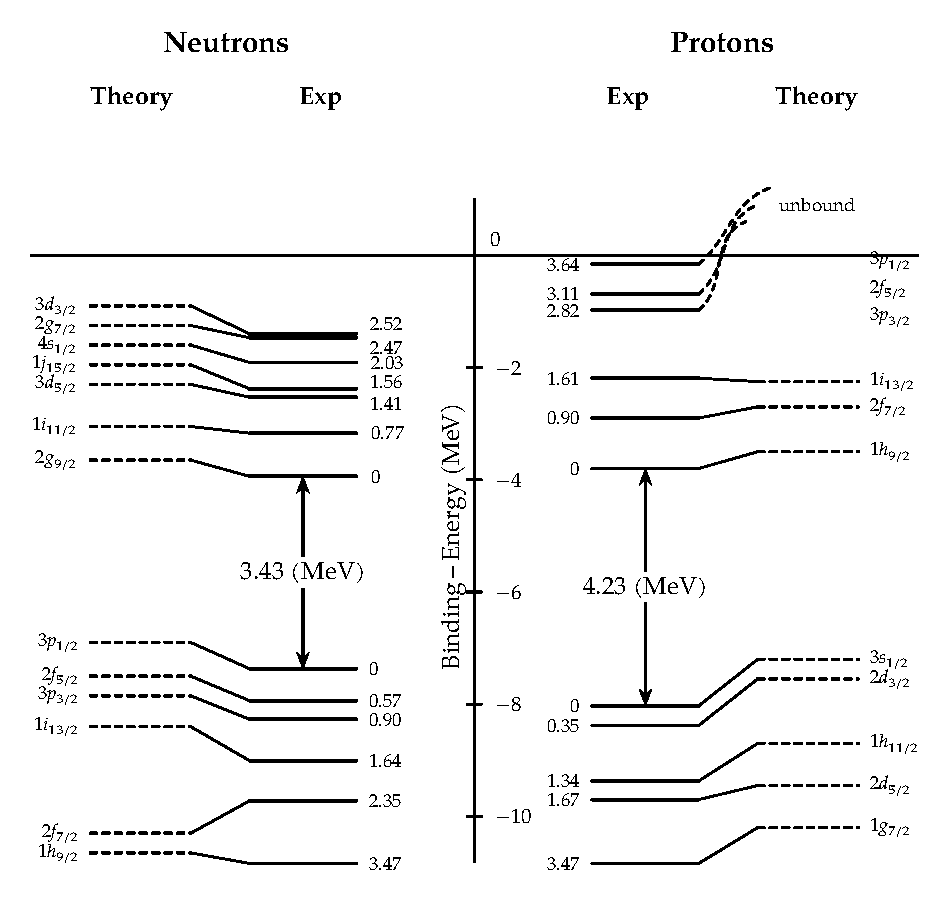
\includegraphics[width=0.75\textwidth]{pictures/2_15}
\par\end{centering}
\caption{\label{fig:2_15}图 2.15 \$\textasciicircum\{208\}}
\end{figure}


\subsection{电磁极矩与跃迁}

单核子电磁极矩与跃迁几率提供了检验核波函数细节的极其敏感的工具（详见附录 B）。

磁偶极矩算符由轨道磁矩与内秉自旋磁矩组成：

\begin{equation}
\boldsymbol{\mu}=\sum^{A}_{i=1}\left(g_{li}\boldsymbol{l}_{i}+g_{si}\boldsymbol{s}_{i}\right)\mu_{N}\label{eq:mag_moment_operator}
\end{equation}

对于单个闭壳外奇核子，在角动量为 $j$ 的状态下计算得到的磁矩被称为 Schmidt 极限（Schmidt limits / Schmidt
lines）\cite{Sc37}：

\begin{align}
\mu & =\left[g_{l}\left(j-\frac{1}{2}\right)+\frac{1}{2}g_{s}\right]\mu_{N},\quad\text{对于 }j=l+\frac{1}{2}\nonumber \\
\mu & =\frac{j}{j+1}\left[g_{l}\left(j+\frac{3}{2}\right)-\frac{1}{2}g_{s}\right]\mu_{N},\quad\text{对于 }j=l-\frac{1}{2}\label{eq:schmidt_limits}
\end{align}

实验测量的磁矩普遍分布在两条 Schmidt 线之间（图 2.17），系统性地小于单粒子预言值（淬灭效应，Quenching）。这一偏差主要源于残余相互作用引起的核芯极化（Core
polarization，即价核子激发闭壳核芯形成粒子-空穴对）以及核子间介子交换流（Meson exchange currents）的贡献。

\begin{figure}[H]
\begin{centering}
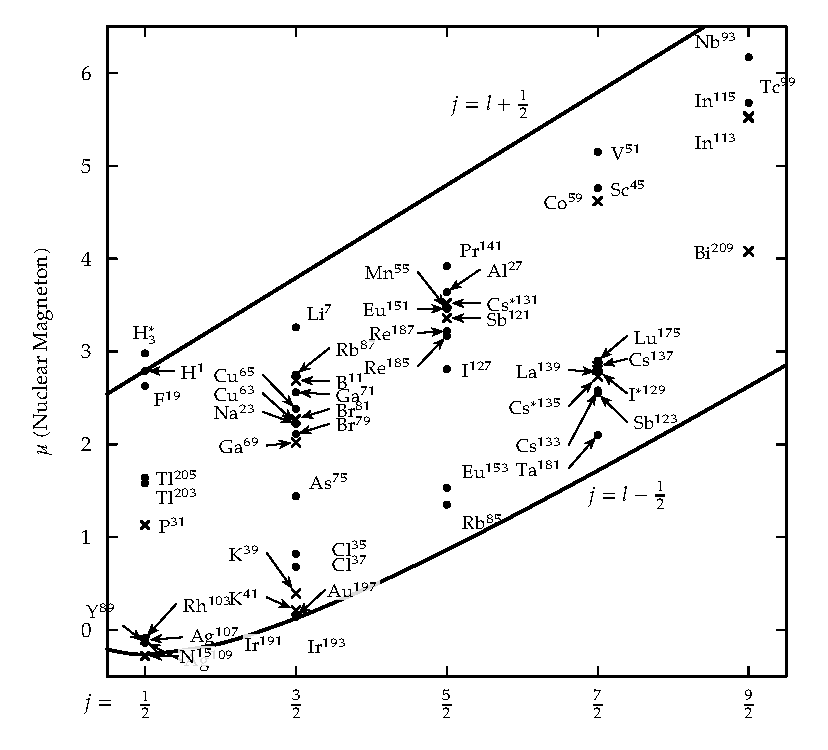
\includegraphics[width=0.75\textwidth]{pictures/2_16}
\par\end{centering}
\caption{\label{fig:2_16}图 2.16 奇 \$Z\$ 核磁矩作为角动量的函数（Schmidt 线，引自 {[}MJ 55{]}）。}
\end{figure}

\begin{figure}[H]
\begin{centering}
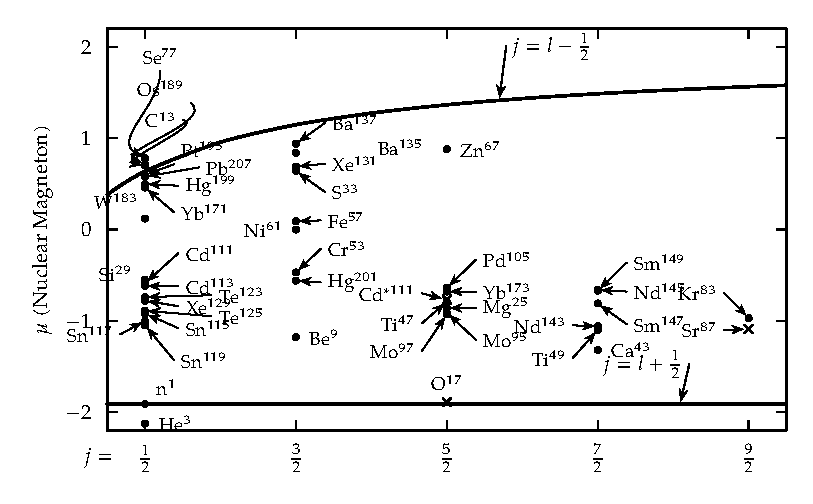
\includegraphics[width=0.75\textwidth]{pictures/2_17}
\par\end{centering}
\caption{\label{fig:2_17}图 2.17 奇 \$N\$ 核磁矩作为角动量的函数（Schmidt 线，引自 {[}MJ 55{]}）。}
\end{figure}

单粒子电四极矩定义为：

\begin{equation}
Q_{\text{s.p.}}=-e_{i}\frac{2j-1}{2(j+1)}\langle r^{2}\rangle\label{eq:single_particle_quadrupole}
\end{equation}

按单纯壳模型，中子不带电（$e_{n}=0$），其实验四极矩应严格为零；而奇质子核的四极矩应由其价质子产生。然而实验测量发现：
\begin{itemize}
\item 奇中子核呈现出明显的非零电四极矩；
\item 奇质子核的实验四极矩比单粒子理论值大近两倍。
\end{itemize}
这一显著效应可以通过引入有效电荷（Effective charge）$e_{\text{eff}}$ 来解释：

\begin{equation}
e_{\text{eff}}=e_{i}+\delta e\label{eq:effective_charge_def}
\end{equation}

其中极化电荷 $\delta e$ 反映了价核子通过两体相互作用将带电核芯极化、激发出虚四极巨共振集体模的效应。在近闭壳核中，典型的极化电荷实验值为：

\begin{equation}
\delta e_{p}\simeq0.5e,\quad\delta e_{n}\simeq0.5e\label{eq:polarization_charge_values}
\end{equation}

由此中子的有效电荷为 $e_{\text{eff}}(n)\simeq0.5e$，质子的有效电荷为 $e_{\text{eff}}(p)\simeq1.5e$。利用这些有效电荷，能够极好地统一解释近闭壳核的静电四极矩以及单粒子电多极跃迁率（以
Weisskopf 单粒子单位 W.u. 衡量）。此外，由于自旋和宇称选择定则的限制，某些高自旋单粒子态只能通过极高多极度的电磁辐射退激发，因而具有极长的寿命，在核素图中形成了著名的“同质异能岛”（Islands
of isomers）。

而在远离闭壳的稀土区和锕系区，实验测量的电四极矩比单粒子预言值大一至两个数量级，且普遍为正值（长椭球形变），清楚表明核芯本身发生了显著的整体稳定形变（图
2.18）。

\begin{figure}[H]
\begin{centering}
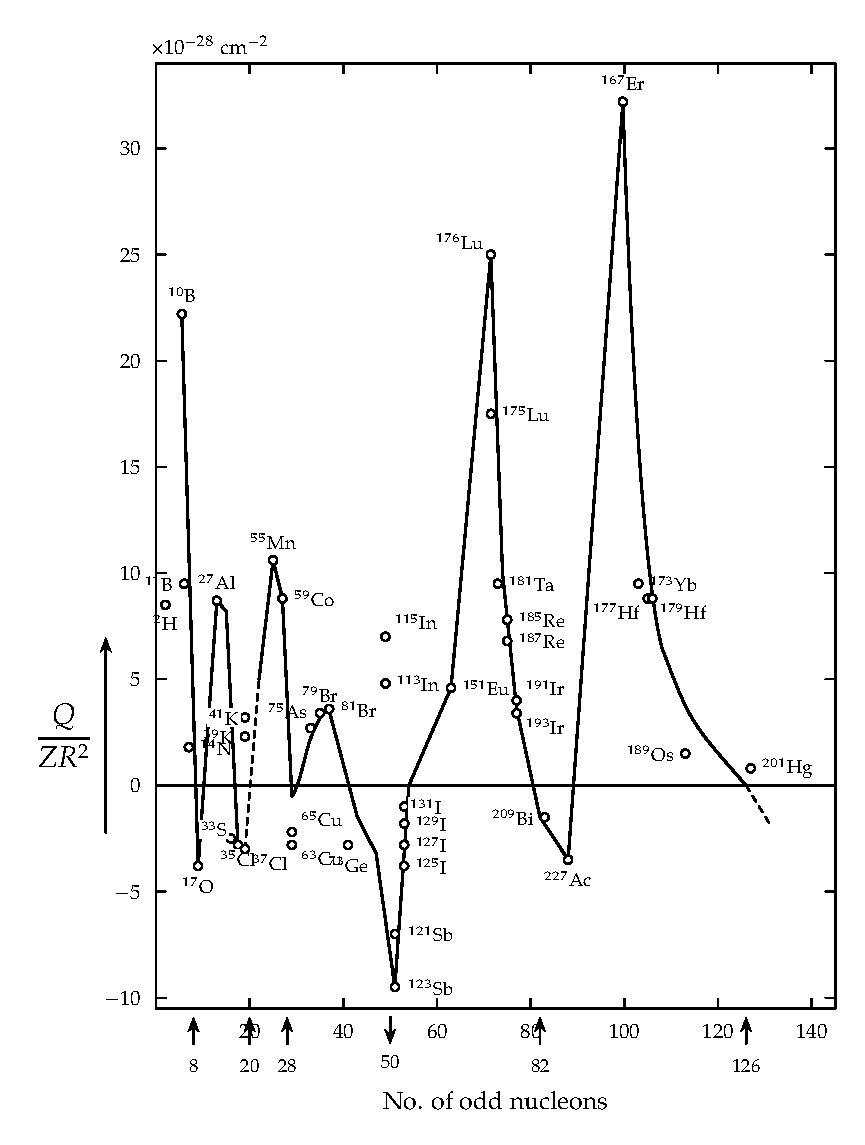
\includegraphics[width=0.75\textwidth]{pictures/2_18}
\par\end{centering}
\caption{\label{fig:2_18}图 2.18 奇 \$A\$ 核电四极矩随奇核子数的变化曲线。箭头标出了满壳位置（引自 {[}Se
64{]}）。}
\end{figure}


\section{形变壳模型\label{sec:=005F62=0053D8=0058F3=006A21=00578B}}

\subsection{实验证据}

在平均势中核子近似独立的运动是壳模型及所有有限核微观理论的基石。在最简单的形式下，该平均势阱被假定为球对称的。这对于闭壳或近闭壳核是高度精确的；然而，当远离闭壳核时，实验观测到了强烈的偏离：
\begin{itemize}
\item 巨大的电四极矩：在稀土区（$150<A<190$）与锕系区（$A>220$），测量到的核基态内秉电四极矩 $Q_{0}$ 比单个未配对核子预期的单粒子值大一到两个数量级（可达数个靶恩，$10^{-24}\,\text{cm}^{2}$）。这意味着有数十个核子协同参与了非球形的形变。
\item 典型的转动能谱：这些核的激发谱呈现出极为规则的转动带序列，其激发能量严格遵循 $E_{I}=\frac{\hbar^{2}}{2\mathcal{J}}I(I+1)$
规律（偶偶核为 $0^{+},2^{+},4^{+},6^{+},\dots$），伴随着极强增强的集体 $E2$ 跃迁（见第 1、3
章）。
\end{itemize}
这些无可辩驳的实验事实清楚地表明，对于开壳层核，原子核的基态自身发生了空间转动对称性的自发破缺，平均场势阱不再保持球形，而形成了固定的空间取向形变。

\subsection{一般的形变势}

描述非球形核表面的普遍方法是将核半径按球谐函数展开：

\begin{equation}
R(\theta,\phi)=R_{0}\left[1+\sum^{\infty}_{\lambda=0}\sum^{\lambda}_{\mu=-\lambda}\alpha^{*}_{\lambda\mu}Y_{\lambda\mu}(\theta,\phi)\right]\label{eq:deformed_surface_expansion}
\end{equation}

其中 $\lambda=1$ 对应质心平移（不改变内秉形状），最重要的多极形变为四极形变 $\lambda=2$。在内秉体固坐标系下，五重分量可由
Hill-Wheeler 形状坐标 $\beta,\gamma$ 参数化（见 1.2 节）：

\begin{align}
a_{20} & =\beta\cos\gamma\nonumber \\
a_{22}=a_{2,-2} & =\frac{1}{\sqrt{2}}\beta\sin\gamma\label{eq:hill_wheeler_beta_gamma}
\end{align}

对于轴对称椭球（$\gamma=0^{\circ}$ 对应长椭球，$\gamma=60^{\circ}$ 对应扁椭球），形变 Woods-Saxon
势具有形式：

\begin{equation}
V(r,\theta,\phi)=-V_{0}\left[1+\exp\left(\frac{r-R(\theta,\phi)}{a(\theta,\phi)}\right)\right]^{-1}\label{eq:deformed_WS_pot}
\end{equation}


\subsection{各向异性谐振子}

若假定形变核的密度为椭球分布，则在谐振子近似下最方便的平均势是各向异性谐振子 Hamilton 量：

\begin{equation}
h_{0}=-\frac{\hbar^{2}}{2m}\nabla^{2}+\frac{m}{2}\left(\omega^{2}_{x}x^{2}+\omega^{2}_{y}y^{2}+\omega^{2}_{z}z^{2}\right)\label{eq:aniso_ho_h0}
\end{equation}

由椭球等势面要求，振荡频率反比于半轴长：$\omega_{\nu}=\omega_{0}\frac{R_{0}}{a_{\nu}}$（$\nu=x,y,z$）。不可压缩流体的体积守恒条件要求：

\begin{equation}
\omega_{x}\omega_{y}\omega_{z}=\text{常数}=\omega^{3}_{0}\label{eq:aniso_ho_vol_conserv}
\end{equation}

本征值为三方向谐振子能量之和：

\begin{equation}
\varepsilon_{0}(n_{x},n_{y},n_{z})=\hbar\omega_{x}\left(n_{x}+\frac{1}{2}\right)+\hbar\omega_{y}\left(n_{y}+\frac{1}{2}\right)+\hbar\omega_{z}\left(n_{z}+\frac{1}{2}\right)\label{eq:aniso_ho_eigenval}
\end{equation}

在轴对称情形下，取 $z$ 轴为对称轴，引入无量纲形变参数 $\delta$：

\begin{align}
\omega^{2}_{\perp}=\omega^{2}_{x}=\omega^{2}_{y} & =\omega^{2}_{0}(\delta)\left(1+\frac{2}{3}\delta\right)\nonumber \\
\omega^{2}_{z} & =\omega^{2}_{0}(\delta)\left(1-\frac{4}{3}\delta\right)\label{eq:aniso_ho_omega_delta}
\end{align}

由体积守恒条件 \ref{eq:aniso_ho_vol_conserv}，展开到 $\delta$ 的二阶可得：

\begin{equation}
\omega_{0}(\delta)=\omega_{0}\left(1+\frac{2}{9}\delta^{2}\right)\label{eq:omega_delta_order2}
\end{equation}

引入形变依赖的特征振子长度 $b(\delta)=\sqrt{\hbar/(m\omega_{0}(\delta))}$ 及无量纲坐标
$\boldsymbol{r}'=\boldsymbol{r}/b(\delta)$，Hamilton 量可表示为球形谐振子加上四极形变扰动项：

\begin{equation}
h_{0}(\delta)=\hbar\omega_{0}(\delta)\left(-\frac{1}{2}\nabla'^{2}+\frac{1}{2}r'^{2}-\frac{1}{3}\sqrt{\frac{16\pi}{5}}\,\delta\,r'^{2}Y_{20}(\theta',\phi')\right)\label{eq:dimensionless_aniso_ho}
\end{equation}

\begin{figure}[H]
\begin{centering}
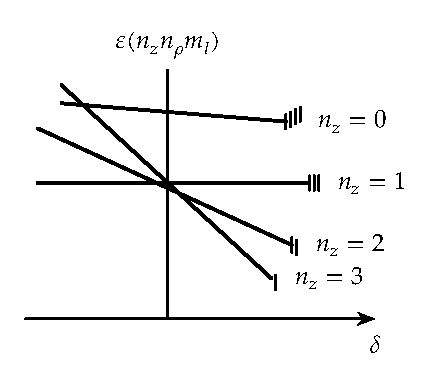
\includegraphics[width=0.75\textwidth]{pictures/2_19}
\par\end{centering}
\caption{\label{fig:2_19}图 2.19 各向异性谐振子能级作为形变参数 \$}
\end{figure}


\subsection{Nilsson Hamilton量}

单纯的形变谐振子势无法给出正确的自旋-轨道劈裂以及重核内部平坦底部的势阱特征。为了在形变核中再现真实的单粒子能谱，Nilsson \cite{Ni55}
在形变谐振子基底上引入了自旋-轨道耦合项与角动量修正项：

\begin{equation}
h=h_{0}(\delta)-\kappa\hbar\omega_{0}\left[2\boldsymbol{l}\cdot\boldsymbol{s}+\mu\left(\boldsymbol{l}^{2}-\langle\boldsymbol{l}^{2}\rangle_{N}\right)\right]\label{eq:nilsson_hamiltonian}
\end{equation}

其中 $\kappa$ 决定了自旋-轨道相互作用的强度，$\mu$ 调节高 $l$ 轨道的相对能量（模拟势阱底部的平坦化），常数
$\langle\boldsymbol{l}^{2}\rangle_{N}=\frac{1}{2}N(N+3)$ 保证各主振子壳层能量重心不发生整体漂移。

\begin{figure}[H]
\begin{centering}
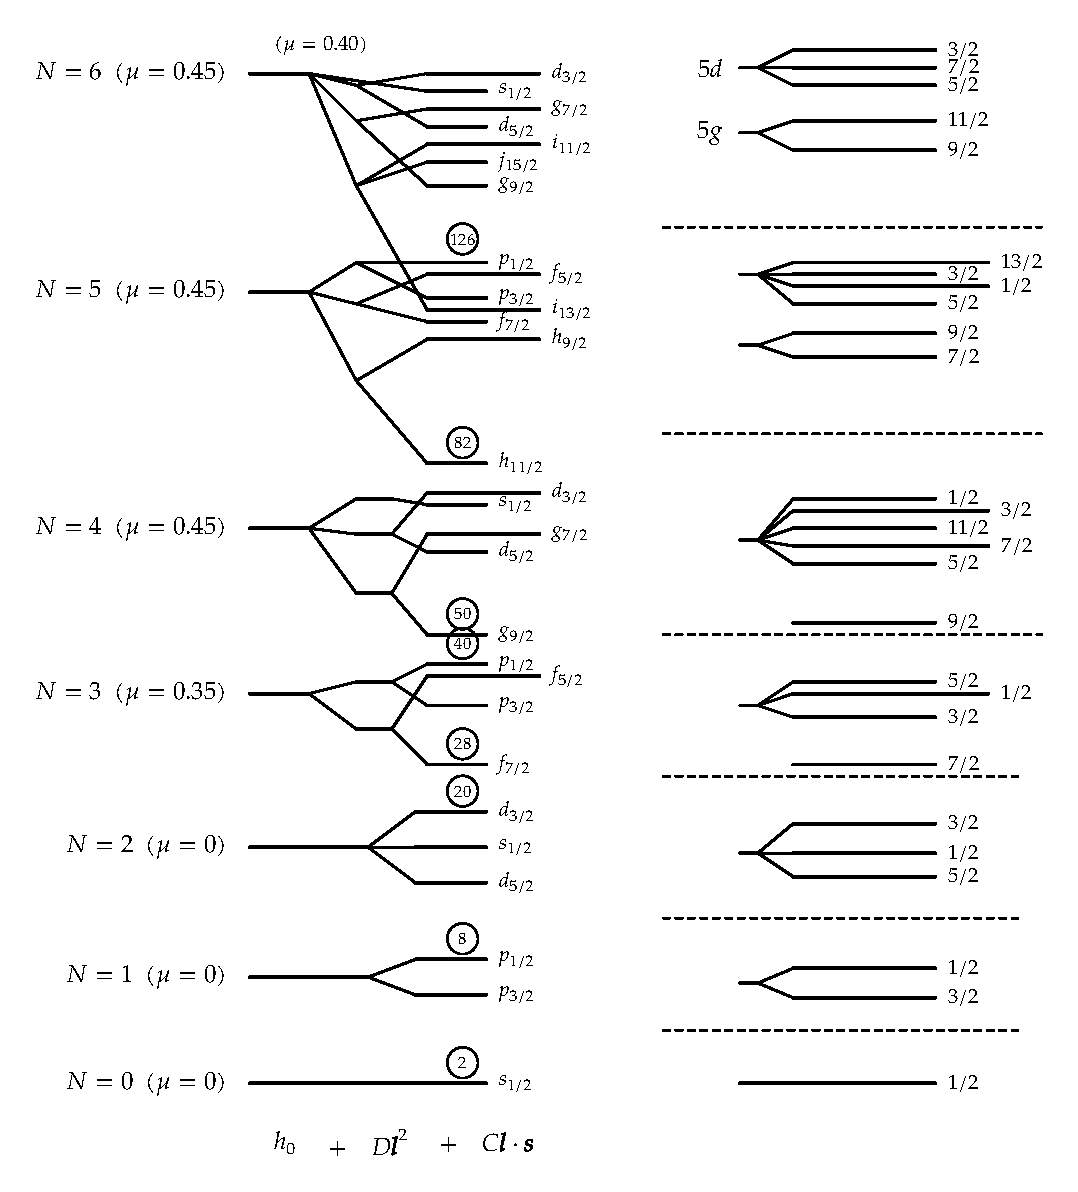
\includegraphics[width=0.75\textwidth]{pictures/2_20}
\par\end{centering}
\caption{\label{fig:2_20}图 2.20 借助 \$}
\end{figure}

由于形变势破坏了全空间转动球对称性，总角动量 $j$ 不再是好量子数。但对于轴对称核，绕对称轴（$z$ 轴）的转动不变性与空间宇称仍然保持守恒。因此总角动量在
$z$ 轴上的投影 $\Omega$ 与空间宇称 $\pi=(-1)^{N}$ 是严格的好量子数：

\begin{equation}
\Omega=j_{z}=l_{z}+s_{z}=\Lambda+\Sigma\label{eq:nilsson_omega_def}
\end{equation}

在大形变极限下，单粒子能级可以用柱坐标下的渐近基量子数 $|Nn_{z}\Lambda\Omega\rangle$（通常简写为渐近标记
$[Nn_{z}\Lambda\Omega]$）标记，其中：
\begin{itemize}
\item $N$：主谐振子量子数；
\item $n_{z}$：沿对称轴方向的振动激发量子数（$n_{z}$ 越大，轨道波函数沿 $z$ 轴越延展，长椭球形变时能量随 $\delta$
下降越快）；
\item $\Lambda$：轨道角动量在 $z$ 轴上的投影（$\Lambda=N-n_{z},N-n_{z}-2,\dots$）；
\item $\Omega=\Lambda\pm1/2$：总角动量在 $z$ 轴上的投影。
\end{itemize}
根据量子力学的不交叉定则（No-crossing rule），具有相同对称性量子数（相同 $\Omega$ 与相同宇称 $\pi$）的能级随形变变化时不会真正相交，而是发生强烈的组态混杂并彼此排斥；只有具有不同
$\Omega$ 或不同宇称的能级才能自由相交。图 2.21 展示了著名的 Nilsson 能级图。

\begin{figure}[H]
\begin{centering}
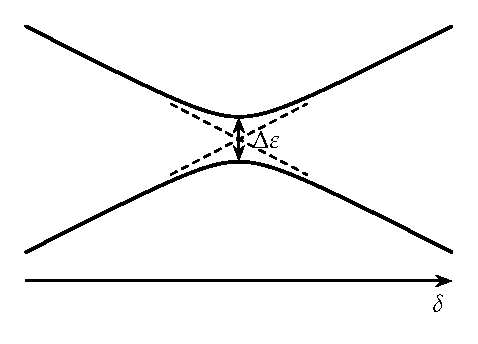
\includegraphics[width=0.75\textwidth]{pictures/2_22}
\par\end{centering}
\caption{\label{fig:2_22}图 2.22 具有相同对称性的两个能级的不相交定则（Neumann-Wigner 定则）。}
\end{figure}

\begin{figure}[H]
\begin{centering}
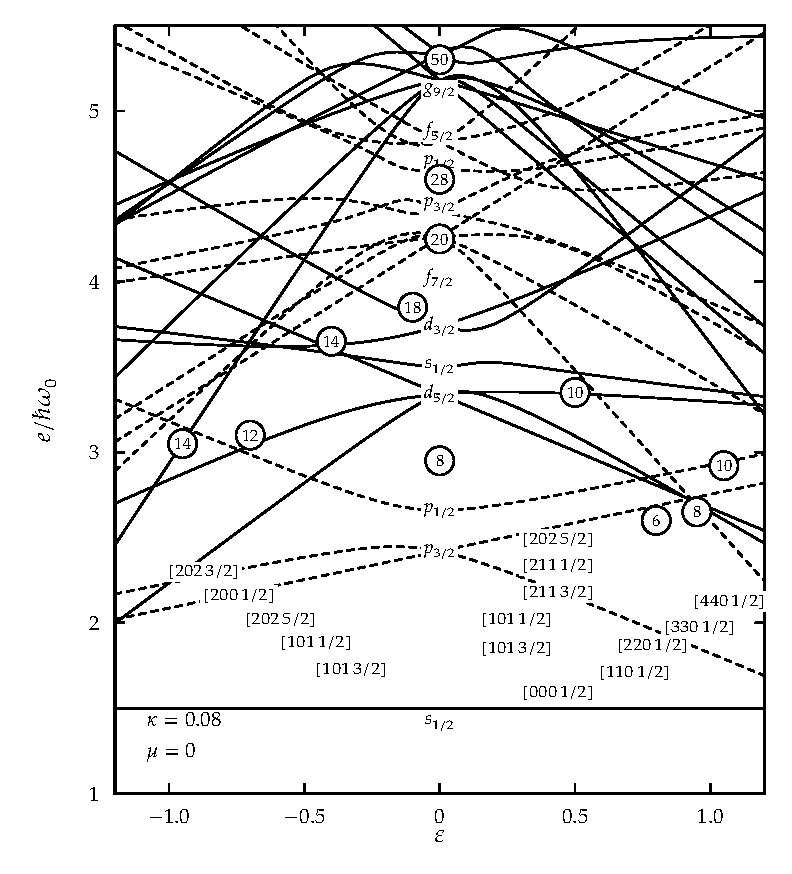
\includegraphics[width=0.75\textwidth]{pictures/2_21a}
\par\end{centering}
\caption{\label{fig:2_21a}图 2.21a 轻核区的 Nilsson 模型单粒子能级图。}
\end{figure}

\begin{figure}[H]
\begin{centering}
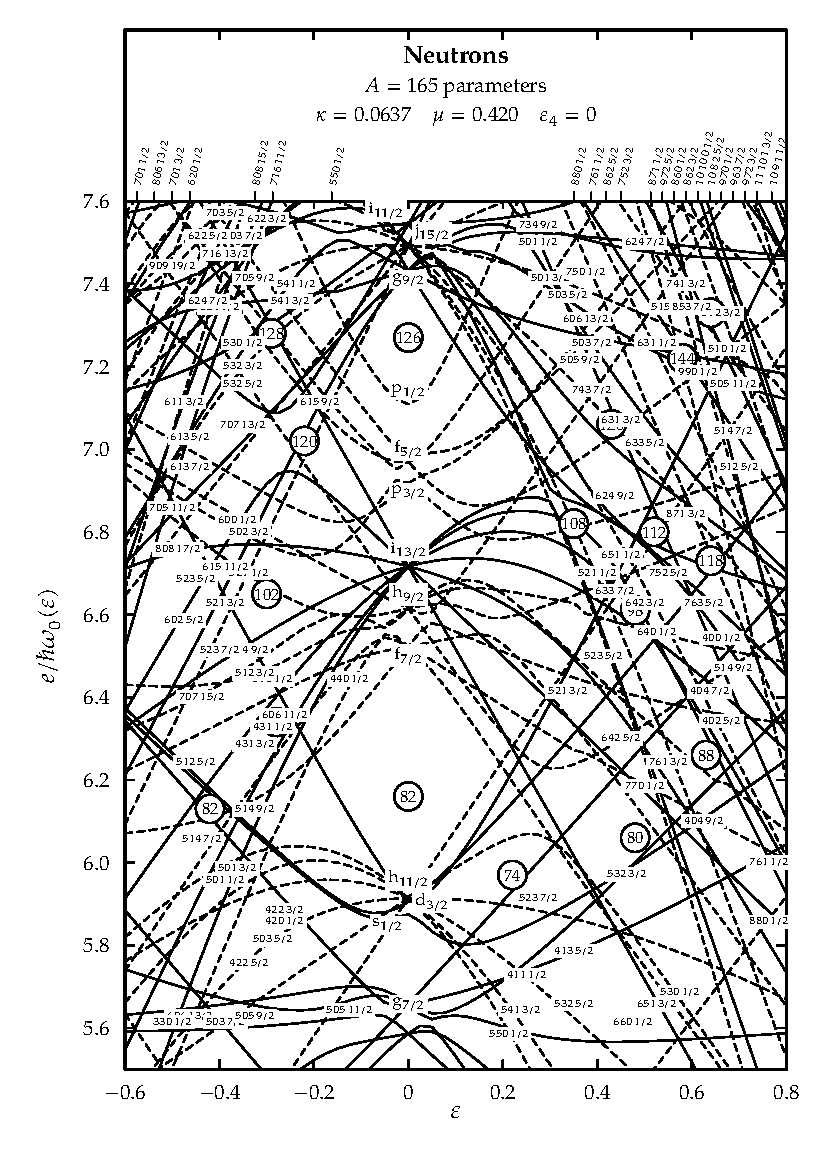
\includegraphics[width=0.75\textwidth]{pictures/2_21b}
\par\end{centering}
\caption{\label{fig:2_21b}图 2.21b 重核区中子的 Nilsson 模型单粒子能级图。}
\end{figure}

\begin{figure}[H]
\begin{centering}
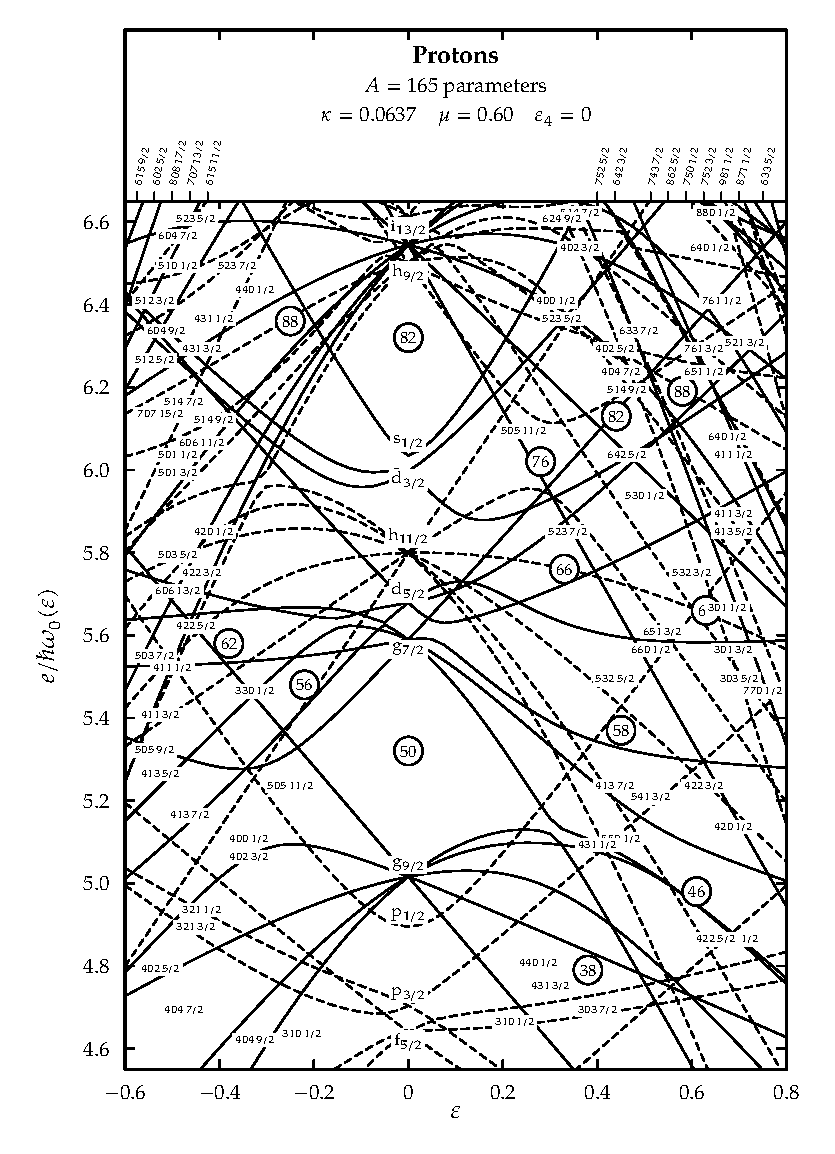
\includegraphics[width=0.75\textwidth]{pictures/2_21c}
\par\end{centering}
\caption{\label{fig:2_21c}图 2.21c 重核区质子的 Nilsson 模型单粒子能级图。}
\end{figure}


\subsection{奇核基态的量子数}

根据时间反演对称性（Kramers 简并），每个形变能级 $\pm\Omega$ 严格二重简并。因此在形变核基态中，所有成对的质子或中子分别以时间反演共轭的方式配对填入
Nilsson 轨道，其总角动量在对称轴上的投影和为零。

对于奇 $A$ 核，最后一个未配对核子占据最高的 Nilsson 能级，因此形变核基态的自旋与宇称完全由该孤立单粒子的 Nilsson
态决定：

\begin{equation}
I=\Omega,\quad\pi=(-1)^{N}\label{eq:nilsson_odd_ground_spin}
\end{equation}

这一简单的定则在稀土区和锕系区的数百个形变奇核中获得了令人惊叹的成功，绝大多数实验测得的基态自旋和宇称均与 Nilsson 能级序列的理论预言完全一致。

\begin{figure}[H]
\begin{centering}
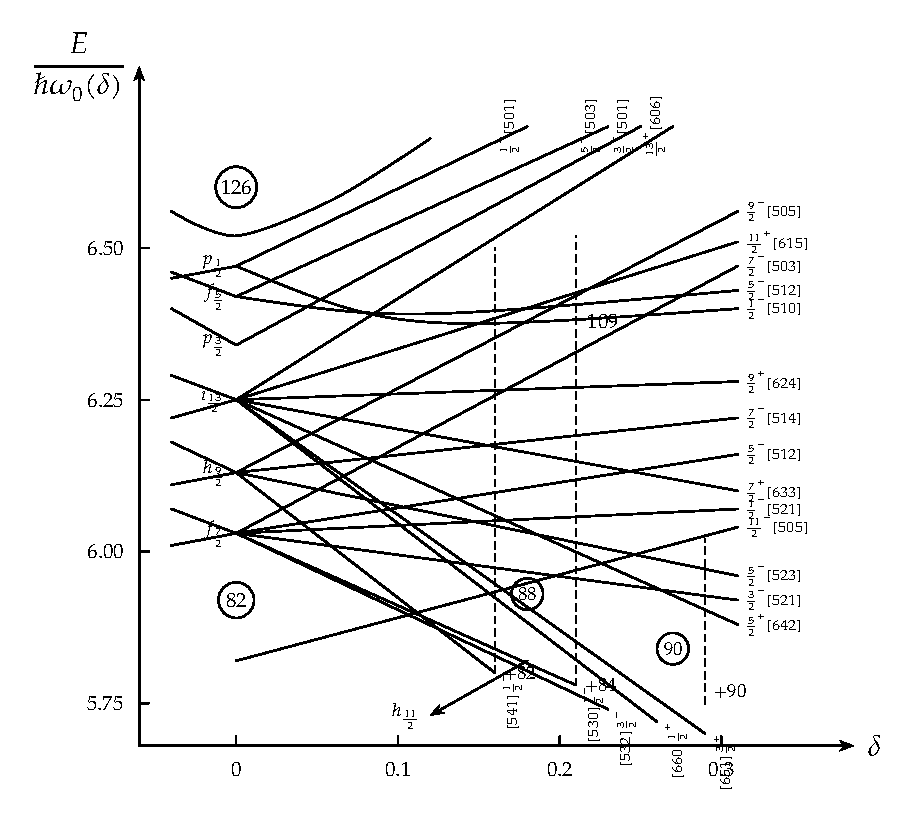
\includegraphics[width=0.75\textwidth]{pictures/2_23}
\par\end{centering}
\caption{\label{fig:2_23}图 2.23 确定奇 \$A\$ 核 \$\textasciicircum\{183\}}
\end{figure}


\subsection{形变能的计算与双中心壳模型}

利用 Nilsson 势最直接的尝试是计算单粒子能量之和随形变参数 $\delta$ 的依赖关系：

\begin{equation}
E_{\text{s.p.}}(\delta)=\sum^{A}_{i=1}\varepsilon_{i}(\delta)\label{eq:sum_single_particle_energy}
\end{equation}

由此寻找能量极小点 $\delta_{\text{eq}}$。虽然这一简单方法对于预测稀土区核的基态平衡形变获得了定性甚至半定量的合理结果（图
2.24），但若将其用于全核素区或大形变行为，就会暴露严重的内在缺陷：

\begin{figure}[H]
\begin{centering}
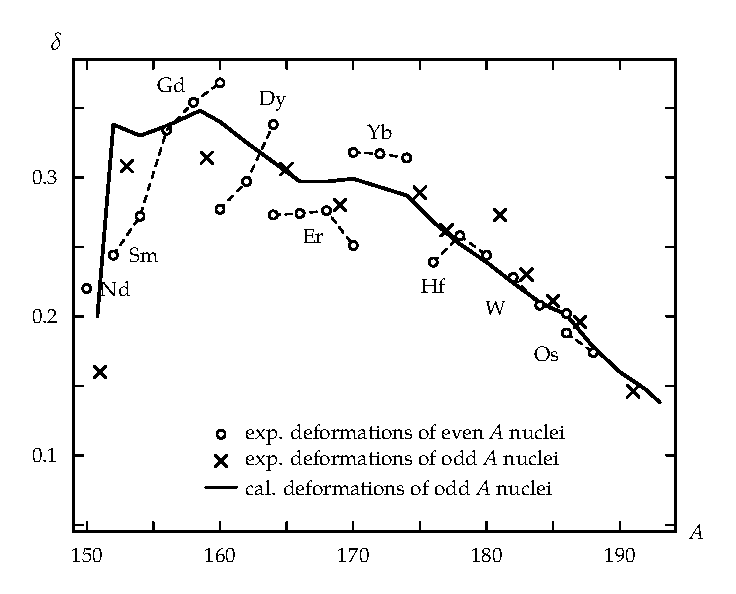
\includegraphics[width=0.75\textwidth]{pictures/2_24}
\par\end{centering}
\caption{\label{fig:2_24}图 2.24 理论计算与实验测定的平衡形变参数比较（引自 {[}MN 55{]}）。}
\end{figure}

\begin{itemize}
\item 能量过度束缚且绝对结合能完全失真：单粒子能量之和 $\sum\varepsilon_{i}$ 重复计算了双体相互作用能（见第 5
章式 (5.28)），导致平均势的体积饱和行为失真；
\item 在大形变与核裂变区域发散：当原子核拉长至发生颈缩、甚至断裂为两个分离的核碎片时，基于单一中心展开的 Nilsson 势完全失去了物理意义。
\end{itemize}
为了描述大形变动力学、重离子聚变与核裂变（Fission）过程，必须构建具有正确渐近极限的形变势模型，其中最重要的代表是双中心壳模型（Two-Center
Shell Model, TCSM）\cite{DR66,HMG69,ADD70,GMG71,MG72}：

双中心模型将平均谐振子势推广为包含两个空间分离中心（位于 $z=\pm z_{0}$）的势阱：

\begin{equation}
V_{\text{TCSM}}(\boldsymbol{r})=\frac{1}{2}m\omega^{2}_{z}(|z|-z_{0})^{2}+\frac{1}{2}m\omega^{2}_{\perp}(x^{2}+y^{2})\label{eq:tcsm_potential}
\end{equation}

当双中心间距 $z_{0}\to0$ 时，势阱平滑过渡为单体复合核的各向异性谐振子势；当 $z_{0}\to\infty$ 时，势阱渐近分解为两个完全独立的单核碎片势。通过在此类具有颈缩参数的双中心势中加入自旋-轨道耦合与形变修正，能够严谨地计算裂变通道上的微观单粒子轨道演化（图
2.25）。类似的大形变势阱还包括折积 Yukawa 势（Folded Yukawa Potential \cite{BFN72,MN73}）和广义形变
Woods-Saxon 势 \cite{BDJ72,Pa73}。

然而，要从这些微观单粒子能级中准确提取真实的形变势能曲面和裂变势垒，必须摒弃粗糙的单粒子能简单求和，而采用宏观-微观结合的 Strutinsky
壳修正方法，这正是下一节的核心主题。

此外在大形变下，微观单粒子壳修正与宏观液滴势垒的叠加，导致能量随形变出现第二极小，完美解释了裂变同质异能现象（图 2.26）。

\begin{figure}[H]
\begin{centering}
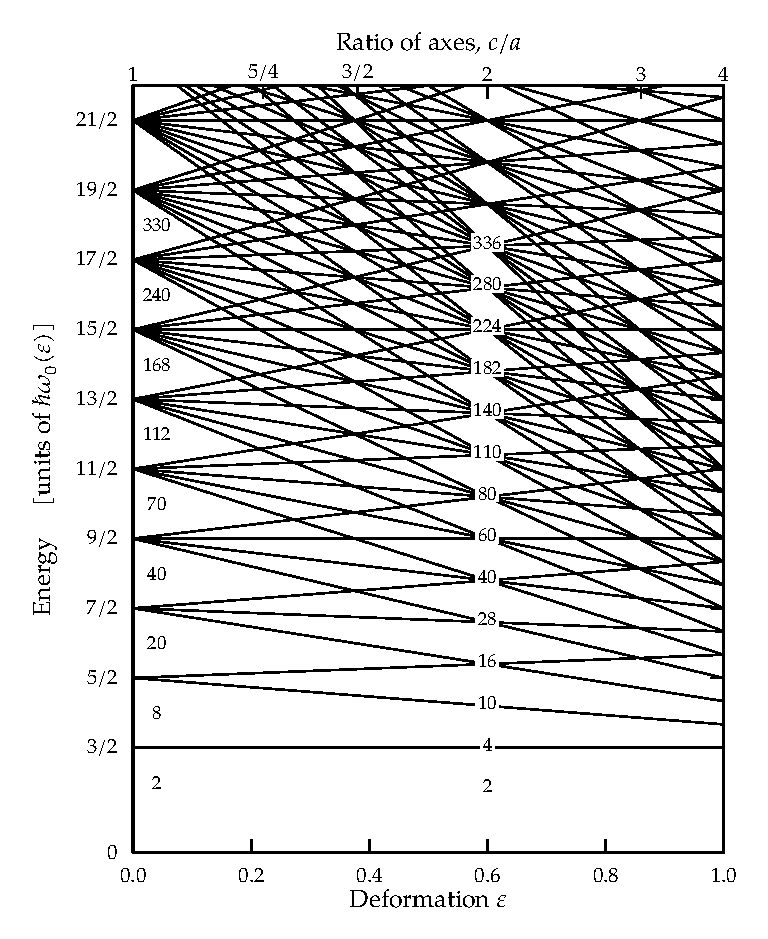
\includegraphics[width=0.75\textwidth]{pictures/2_25}
\par\end{centering}
\caption{\label{fig:2_25}图 2.25 长椭球形变谐振子势中的单粒子能级随形变 \$}
\end{figure}

\begin{figure}[H]
\begin{centering}
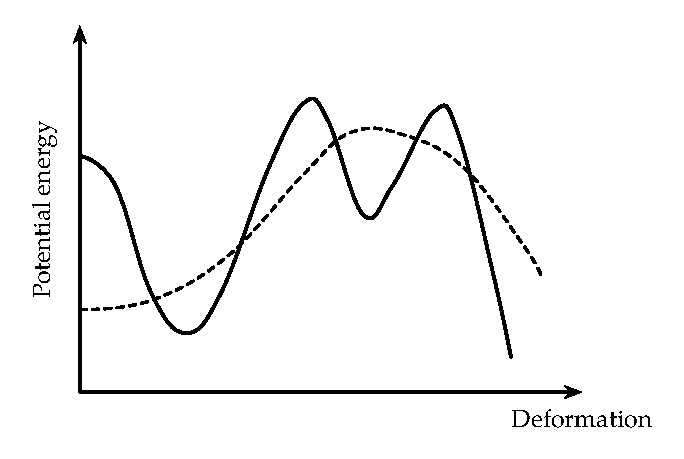
\includegraphics[width=0.75\textwidth]{pictures/2_26}
\par\end{centering}
\caption{\label{fig:2_26}图 2.26 具有第二极小的原子核能量随形变变化的示意图。虚线对应纯液滴模型势垒。}
\end{figure}


\section{液滴模型的壳修正与 Strutinsky 方法\label{sec:=006DB2=006EF4=006A21=00578B=007684=0058F3=004FEE=006B63}}

\subsection{引言}

在第 1 章中我们看到，液滴模型能够极好地再现结合能的平均行为。然而，在幻数附近结合能存在明显的偏离（见图 2.2），这一事实清楚地表明了单粒子壳效应的存在。另一方面，虽然唯象壳模型能够成功解释基态自旋、宇称以及低激发谱的单粒子性质，但如果仅仅将独立单粒子能级之和作为核的总结合能，在定量上却无法给出正确的核物质饱和性质与绝对结合能（如
2.8.6 节所述）。

为了克服这一困难，Strutinsky \cite{St67,St68} 提出了一个非常富有成果的微观-宏观结合方法（宏观-微观方法）。其基本物理图像是：总结合能可以分解为一个平滑变化的大体部分（即宏观液滴模型能量）加上一个由单粒子能级非均匀分布引起的微小涨落修正部分（即微观壳修正能）：

\[
E=E_{\text{LDM}}+E_{\text{osc}}
\]

这种分解基于如下事实：结合能的平均行为主要由平滑的平均能级密度决定，而液滴模型已经通过唯象参数的拟合极好地包含了这部分宏观体积和表面能量；唯象壳模型中不准确的正是其平滑宏观部分，但它却相当精确地给出了
Fermi 能量附近的能级成团结构（即壳效应）。因此，我们只需利用壳模型计算振荡修正量 $E_{\text{osc}}$，并将其加到宏观的液滴模型能量
$E_{\text{LDM}}$ 之上。

\subsection{Strutinsky 平均方法的基本思想}

\begin{figure}[H]
\begin{centering}
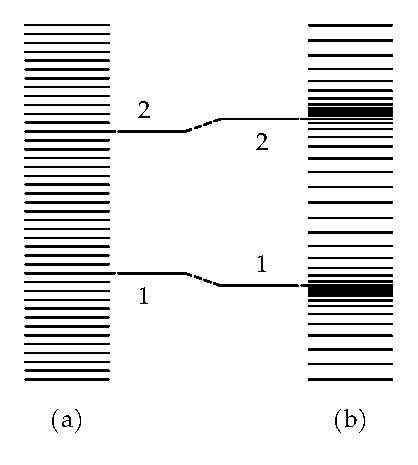
\includegraphics[width=0.75\textwidth]{pictures/2_27}
\par\end{centering}
\caption{\label{fig:2_27}图 2.27 等间距能级密度与示意壳模型聚束能级密度的比较。}
\end{figure}

为了在数学上严谨地定义振荡能量 $E_{\text{osc}}$，首先需要将壳模型的单粒子能级密度 $g(\varepsilon)=\sum_{i}\delta(\varepsilon-\varepsilon_{i})$
分解为平滑部分 $\tilde{g}(\varepsilon)$ 与振荡涨落部分 $\delta g(\varepsilon)$：

\begin{equation}
g(\varepsilon)=\tilde{g}(\varepsilon)+\delta g(\varepsilon)\label{eq:strut_g_decomp}
\end{equation}

由平滑能级密度 $\tilde{g}(\varepsilon)$，可以通过核子数守恒条件唯一定义平滑的化学势（即平均 Fermi
能）$\tilde{\lambda}$：

\begin{equation}
A=\int^{\tilde{\lambda}}_{-\infty}\tilde{g}(\varepsilon)\,\mathrm{d}\varepsilon\label{eq:strut_lambda_tilde}
\end{equation}

由此可得壳模型的平滑能量贡献：

\begin{equation}
\tilde{E}_{\text{sh}}=\int^{\tilde{\lambda}}_{-\infty}\varepsilon\,\tilde{g}(\varepsilon)\,\mathrm{d}\varepsilon\label{eq:strut_E_smooth}
\end{equation}

而单纯单粒子壳模型给出的基态能量为：

\begin{equation}
E_{\text{sh}}=\sum^{A}_{i=1}\varepsilon_{i}\label{eq:strut_E_sh}
\end{equation}

因此，由于壳层非均匀聚集导致的能量涨落（壳修正能）即为二者之差：

\begin{equation}
E_{\text{osc}}=E_{\text{sh}}-\tilde{E}_{\text{sh}}\label{eq:strut_E_osc_def}
\end{equation}

由此体系的总能量表示为：

\begin{equation}
E=E_{\text{LDM}}+E_{\text{sh}}-\tilde{E}_{\text{sh}}\label{eq:strut_total_E}
\end{equation}

在液滴模型中，稳定的平衡核形状总是球对称的。但由于额外的壳修正项 $E_{\text{osc}}$ 随形变剧烈振荡，在核素表的许多区域（如稀土区与锕系区），Strutinsky
平均能量式 \ref{eq:strut_total_E} 的能量极小值将落在非零的形变处，从而自然地解释了原子核的自发四极形变。

\subsection{平均能级密度的确定}

现在我们探讨如何从给定的离散单粒子能级谱 $g(\varepsilon)=\sum_{i}\delta(\varepsilon-\varepsilon_{i})$
中，以严格的数学方式提取其平滑部分 $\tilde{g}(\varepsilon)$。困难在于三维势阱中的能级密度随能量呈现非线性增长，且聚集成间距约为
$\hbar\omega_{0}$ 的壳层。通常的想法是将能级密度与一个平滑函数 $f(x)$ 进行折积：

\begin{equation}
\tilde{g}(\varepsilon)=\frac{1}{\gamma}\int^{+\infty}_{-\infty}g(\varepsilon')f\left(\frac{\varepsilon'-\varepsilon}{\gamma}\right)\,\mathrm{d}\varepsilon'\label{eq:strut_folding}
\end{equation}

\begin{figure}[H]
\begin{centering}
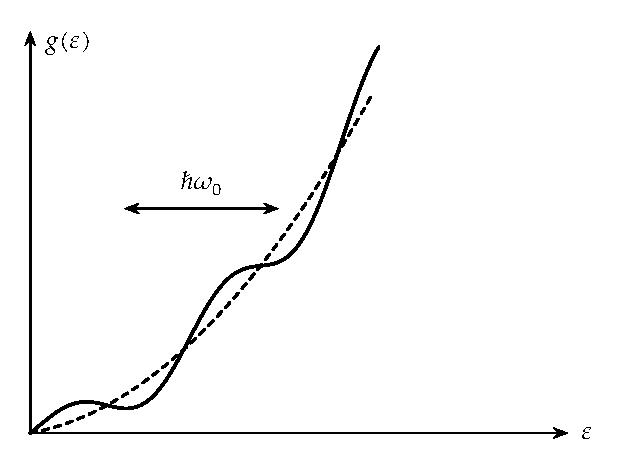
\includegraphics[width=0.75\textwidth]{pictures/2_28}
\par\end{centering}
\caption{\label{fig:2_28}图 2.28 三维无限深势阱中能级密度的示意图（展示离散尖峰能级密度与平滑平均能级密度）。}
\end{figure}

其中 $\gamma$ 为平滑宽度，其大小取为主壳层间隔量级（$\gamma\simeq\hbar\omega_{0}$）。然而单纯取
$f$ 为纯 Gauss 函数并不充分，因为合理的平滑程序必须满足自洽重平均不变性：若对已经平滑的能级密度 $\tilde{g}$
再次施行相同的平滑操作，其结果应保持不变：

\begin{equation}
\tilde{g}(\varepsilon)=\frac{1}{\gamma}\int^{+\infty}_{-\infty}\tilde{g}(\varepsilon')f\left(\frac{\varepsilon'-\varepsilon}{\gamma}\right)\,\mathrm{d}\varepsilon'\label{eq:strut_self_consistent}
\end{equation}

当 $f$ 为纯 Gauss 函数而 $\tilde{g}$ 包含多项式曲率时，式 \ref{eq:strut_self_consistent}
并不严格成立。由于积分的主要贡献来自于 $\varepsilon'=\varepsilon$ 的近邻区域，我们假定平滑密度 $\tilde{g}(\varepsilon')$
在局域上可以被一个 $2M$ 阶的多项式很好地逼近（通常取 $2M=2,4,6$）。此时若将平滑函数取为多项式与加权因子的乘积：

\begin{equation}
f(x)=P(x)w(x)\label{eq:strut_f_pw}
\end{equation}

其中 $P(x)$ 为 $2M$ 阶偶多项式（曲率修正多项式），$w(x)$ 为 Gauss 加权函数：

\begin{equation}
w(x)=\frac{1}{\sqrt{\pi}}e^{-x^{2}}\label{eq:strut_gauss_w}
\end{equation}

通过正交多项式理论 \cite{AS65}，$P(x)$ 可以由 Hermite 多项式精确构建：

\begin{equation}
P(x)=\sum^{M}_{n=0}\frac{(-1)^{n}}{2^{2n}n!}H_{2n}(x)=L^{1/2}_{M}(x^{2})\label{eq:strut_laguerre}
\end{equation}

这里 $L^{1/2}_{M}(x^{2})$ 是伴随 Laguerre 多项式。展开为幂级数形式：

\begin{equation}
L^{1/2}_{M}(x^{2})=\sum^{M}_{n=0}a_{2n}x^{2n}\label{eq:strut_laguerre_poly}
\end{equation}

在实际计算中常用的前四阶系数如表 2.5 所示。

\begin{table}[htbp]
\caption{\label{tab:laguerre_coefficients}前四个 Laguerre 多项式系数}

\centering{}%
\begin{tabular}{ccccc}
\hline 
$M$ & $a_{0}$ & $a_{2}$ & $a_{4}$ & $a_{6}$\tabularnewline
\hline 
0 & 1 & — & — & —\tabularnewline
1 & 3/2 & -1 & — & —\tabularnewline
2 & 15/8 & -5/2 & 1/2 & —\tabularnewline
3 & 35/16 & -35/8 & 7/4 & -1/6\tabularnewline
\hline 
\end{tabular}
\end{table}

接下来需要确定平滑参数 $\gamma$ 与曲率阶数 $M$ 的具体取值。物理上有意义的平均方法必须要求最终计算出的物理量在很大程度上独立于平滑参数的选择。这意味着对于固定的
$M$，平均能量 $\tilde{E}_{\text{sh}}$ 随 $\gamma$ 的变化必须存在一个平坦的“坪区”（Plateau），在该区域内严格满足坪区条件
\cite{BP73}：

\begin{equation}
\frac{\partial\tilde{E}_{\text{sh}}}{\partial\gamma}=0\label{eq:strut_plateau}
\end{equation}

由于真实核能级总是以大约 $\hbar\omega_{0}$ 的间距成团，只要取 $\gamma\simeq(1.0\sim1.5)\hbar\omega_{0}$
且 $M\geqslant2$，在绝大多数核物理问题中均能观察到极为宽阔稳定的能量坪区。第 13 章将进一步证明，Strutinsky
平滑方法在深层次上与半经典 Thomas-Fermi 近似完全等价。

\begin{figure}[H]
\begin{centering}
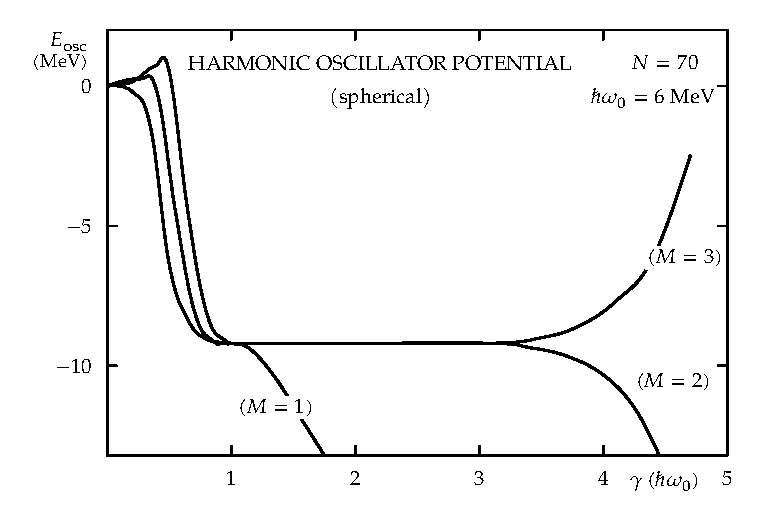
\includegraphics[width=0.75\textwidth]{pictures/2_30}
\par\end{centering}
\caption{\label{fig:2_30}图 2.30 谐振子势的壳修正能作为平滑宽度 \$}
\end{figure}


\subsection{Strutinsky 壳修正能的计算}

利用确定的平滑函数 $f(x)$，由离散谱 $g(\varepsilon)=\sum_{i}\delta(\varepsilon-\varepsilon_{i})$
得到的平滑能级密度为：

\begin{equation}
\tilde{g}(\varepsilon)=\sum_{i}\frac{1}{\gamma}f\left(\frac{\varepsilon-\varepsilon_{i}}{\gamma}\right)\label{eq:strut_g_smooth_sum}
\end{equation}

将其代入粒子数积分，可引入广义占据数 $\tilde{n}_{i}$：

\begin{equation}
A=\sum_{i}\tilde{n}_{i}=\sum_{i}\int^{t_{i}}_{-\infty}f(x)\,\mathrm{d}x,\quad t_{i}=\frac{\tilde{\lambda}-\varepsilon_{i}}{\gamma}\label{eq:strut_n_tilde}
\end{equation}

由此平滑能量可写为：

\begin{equation}
\tilde{E}_{\text{sh}}=\sum_{i}\varepsilon_{i}\tilde{n}_{i}+F\label{eq:strut_E_smooth_F}
\end{equation}

其中残余项 $F$ 为：

\begin{equation}
F=\sum_{i}\int^{\tilde{\lambda}}_{-\infty}(\varepsilon-\varepsilon_{i})\frac{1}{\gamma}f\left(\frac{\varepsilon-\varepsilon_{i}}{\gamma}\right)\,\mathrm{d}\varepsilon=\gamma\sum_{i}\int^{t_{i}}_{-\infty}xf(x)\,\mathrm{d}x\label{eq:strut_F_def}
\end{equation}

对平滑能量对 $\gamma$ 求导可得：

\begin{equation}
\frac{\partial\tilde{E}_{\text{sh}}}{\partial\gamma}=\frac{1}{\gamma}F+\tilde{\lambda}\frac{\partial}{\partial\gamma}\sum_{i}\tilde{n}_{i}=\frac{1}{\gamma}F+\tilde{\lambda}\frac{\partial A}{\partial\gamma}=\frac{1}{\gamma}F\label{eq:strut_dE_dgamma}
\end{equation}

由于核子数 $A$ 严格守恒（$\partial A/\partial\gamma=0$），坪区条件 $\partial\tilde{E}_{\text{sh}}/\partial\gamma=0$
恰好等价于 $F=0$！定义纯壳模型的阶梯占据数：

\begin{equation}
n_{i}=\begin{cases}
1, & \varepsilon_{i}\leqslant\varepsilon_{F}\\
0, & \varepsilon_{i}>\varepsilon_{F}
\end{cases}\label{eq:strut_step_n}
\end{equation}

则总壳修正能 $E_{\text{osc}}$ 可以极为优美简洁地表示为占据数偏差 $\delta n_{i}=n_{i}-\tilde{n}_{i}$
的单粒子能级加权和：

\begin{equation}
E_{\text{osc}}=\sum_{i}\varepsilon_{i}(n_{i}-\tilde{n}_{i})=\sum_{i}\varepsilon_{i}\delta n_{i}\label{eq:strut_E_osc_final}
\end{equation}

\begin{figure}[H]
\begin{centering}
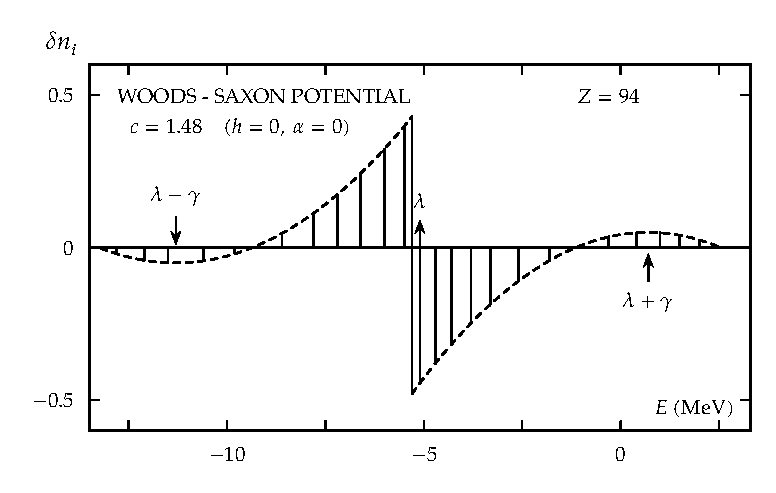
\includegraphics[width=0.75\textwidth]{pictures/2_29}
\par\end{centering}
\caption{\label{fig:2_29}图 2.29 采用 Strutinsky 平均方法对 Woods-Saxon 势计算得到的占有数偏差
\$}
\end{figure}

由占据数偏差量 $\delta n_{i}$，还可以直接计算坐标表象中的微观单体密度壳修正 \cite{Di71}：

\begin{equation}
\delta\rho_{\text{osc}}(\boldsymbol{r},\boldsymbol{r}')=\sum_{i}\phi_{i}(\boldsymbol{r})\phi^{*}_{i}(\boldsymbol{r}')\delta n_{i}\label{eq:strut_delta_rho}
\end{equation}

对于重核，核子对关联（见第 6、7 章）也扮演着重要角色。在 BCS 理论下，对能 $P$ 同样与 Fermi 面附近的能级密度紧密相关。由于宏观液滴能量已拟合了平均质量，其本身已包含了对能的平滑宏观部分
$\tilde{P}_{\text{BCS}}$，因此只需额外加上对能的振荡修正 $P_{\text{osc}}=P_{\text{BCS}}-\tilde{P}_{\text{BCS}}$。最终核体系的总形变能量由下式给出：

\begin{equation}
E=E_{\text{LDM}}+E_{\text{sh}}-\tilde{E}_{\text{sh}}+P_{\text{BCS}}-\tilde{P}_{\text{BCS}}\label{eq:strut_total_E_pairing}
\end{equation}


\subsection{壳修正与 Hartree-Fock 方法}

在第 5 章中我们将详细探讨如何从微观现实核力通过 Hartree-Fock（HF）方法自洽求解微观平均场。在此我们简要说明：Strutinsky
壳修正方法并非唯象拼凑，而是具有坚实的微观理论基础。

在 HF 理论中，基态总能量以表象无关的方式表示为：

\begin{equation}
E^{\text{HF}}_{0}=\mathrm{Tr}(t\rho)+\frac{1}{2}\mathrm{Tr}_{1}\mathrm{Tr}_{1}\rho\bar{v}\rho\label{eq:strut_E_HF}
\end{equation}

其中 $\rho$ 为自洽单粒子密度矩阵，$h^{\text{HF}}=t+\mathrm{Tr}_{1}\bar{v}\rho$
为单粒子 HF Hamilton 量。将自洽密度分解为平滑部分与振荡部分：

\begin{equation}
\rho=\tilde{\rho}+\delta\rho\label{eq:strut_rho_decomp}
\end{equation}

代入能量表达式并按 $\delta\rho$ 的阶数展开：

\begin{equation}
E^{\text{HF}}_{0}=\tilde{E}+\mathrm{Tr}(\tilde{h}^{\text{HF}}\delta\rho)+\mathcal{O}((\delta\rho)^{2})\label{eq:strut_energy_theorem}
\end{equation}

其中 $\tilde{E}=\mathrm{Tr}(t\tilde{\rho})+\frac{1}{2}\mathrm{Tr}_{1}\mathrm{Tr}_{1}\tilde{\rho}\bar{v}\tilde{\rho}$
正好对应于宏观液滴能量，而 $\tilde{h}^{\text{HF}}=t+\mathrm{Tr}_{1}\bar{v}\tilde{\rho}$
为由平滑密度生成的平均单体 Hamilton 量。注意到一阶变分项 $\mathrm{Tr}(\tilde{h}^{\text{HF}}\delta\rho)$
正好对应于式 \ref{eq:strut_E_osc_final} 的单粒子能谱求和修正！式 \ref{eq:strut_energy_theorem}
被称为 Strutinsky 能量定理（Strutinsky Energy Theorem）\cite{St68,St74}：它证明了在
$\delta\rho$ 的一阶精度下，微观自洽多体理论的所有壳效应均完全包含在平均势单粒子能级的求和之中，而二阶修正项 $\mathcal{O}((\delta\rho)^{2})$
极小（经数值计算验证通常小于 1 MeV \cite{BKS72,BQ75a}）。

\begin{figure}[H]
\begin{centering}
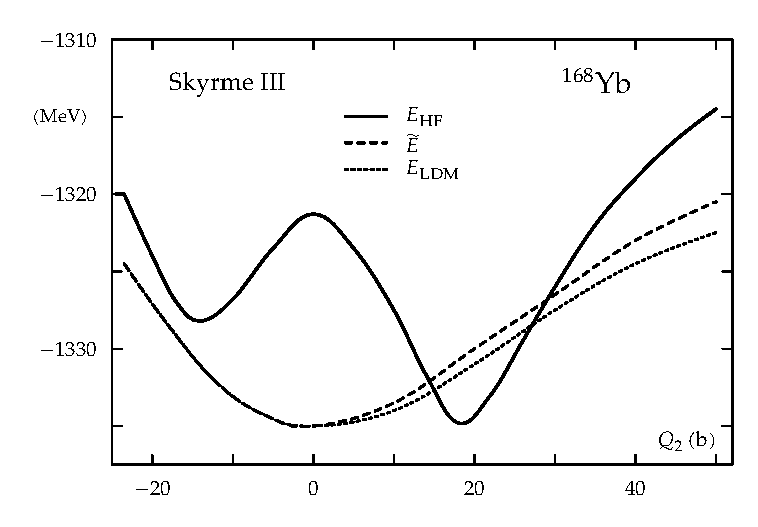
\includegraphics[width=0.75\textwidth]{pictures/2_31}
\par\end{centering}
\caption{\label{fig:2_31}图 2.31 采用 Skyrme III 力计算的 \$\textasciicircum\{168\}}
\end{figure}


\subsection{若干应用}

Strutinsky 壳修正理论在核物理中取得了巨大的成功：
\begin{enumerate}
\item 核质量与结合能：结合液滴模型与 Nilsson 势壳修正，极为成功地再现了全核素区核质量系统学（图 2.32 \cite{NTT69}），尤其精准再现了双幻核
$\ce{^{208}Pb}$ 附近的结合能剧烈振荡结构。
\end{enumerate}
\begin{figure}[H]
\begin{centering}
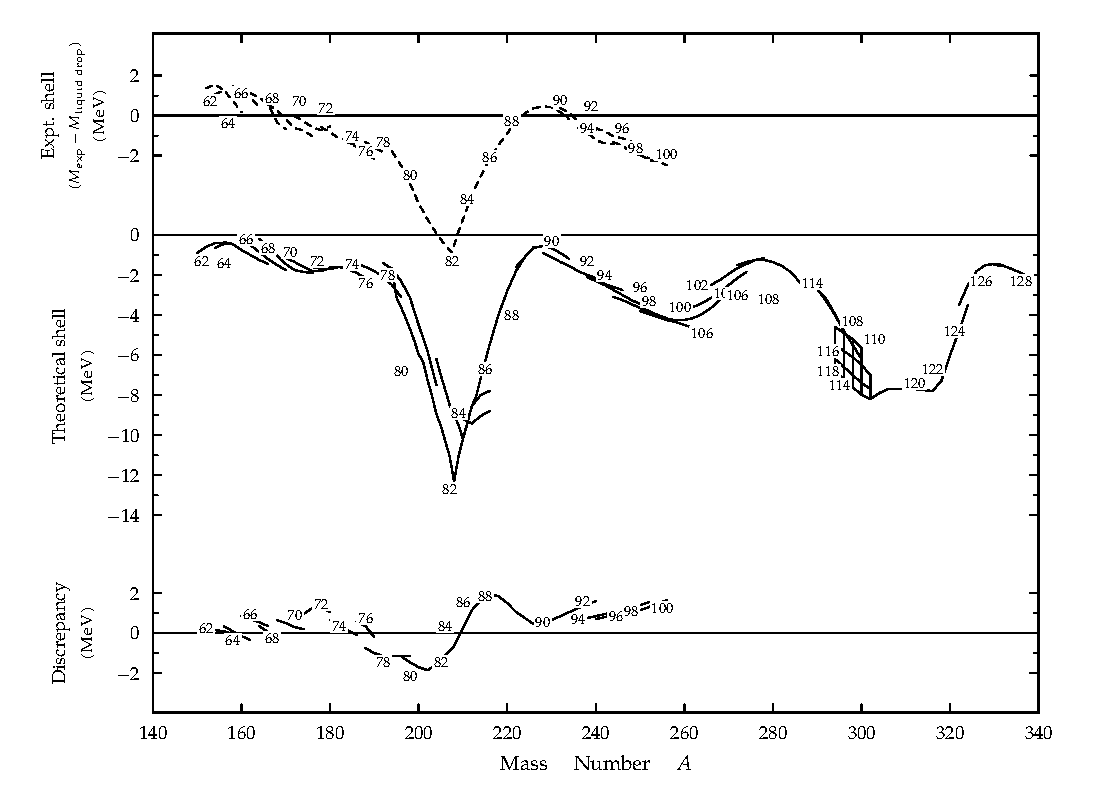
\includegraphics[width=0.75\textwidth]{pictures/2_32}
\par\end{centering}
\caption{\label{fig:2_32}图 2.32 理论计算的质量修正与全核素区实验值的比较（引自 {[}NTT 69{]}）。}
\end{figure}

\begin{enumerate}
\item 多维形变能曲面与双峰裂变势垒：不仅考虑四极形变，还将八极形变、十六极形变等纳入考虑，构建多维形变能曲面。在锕系核中成功预言了双峰裂变势垒（Double-humped
fission barrier），并解释了处于第二极小势阱中的形变同质异能态（裂变同质异能素，fission isomers）。
\item 裂变半衰期与超重核稳定性：通过在多维势能曲面上寻找跨越最低势垒的动力学路径，定量计算重核与超重核的自发裂变寿命，奠定了现代超重核稳定岛（Island
of Stability）预言的理论基石 \cite{Ni72,NN74,BN77}。
\end{enumerate}




\chapter{转动与单粒子运动}

\section{引言}

在实验的水平上，原子核内部的相关机制显示出了极大的复杂性。即使是为了研究原子核最基本的性质，我们也不得不在本书的前两章介绍了两种几乎截然不同的方法：一方面，液滴模型描述了包含许多核子的体系的集体行为，例如振动和转动；另一方面，壳模型将每个核子视作独立的粒子，从而加深了我们对单粒子激发的认识。然而，这两个模型在研究中是受限的，因为自然界中不存在严格满足这样模型的体系。真实的系统总是对模型存在偏离，因此我们不得不考察这些极端模型之间的转变关系。

为了获得对于原子核内部结构的更深刻认识，原则上来说我们需要求解原子核多体问题，并且研究在极限情况下的解对应的物理图像；以及判断何时我们需要提出新的模型来得到对原子核体系的简介描述。在这本书接下来的章节中，我们会从更加微观的角度来研究这些微观方法，并且复现这些唯象模型的结果。尽管这些模型能够帮助我们厘清一些原理性的问题，由于它们通常包含了难以处理的数值计算量，因此在快速定量地解释实验现象上它们并不是十分有效。

因此，在这一章沿着唯象道路的继续探索以及努力将单粒子模型和集体模型结合起来描述更复杂的谱看起来是有价值的。在上一章中我们看到，这样的结合对于描述结合能和形变这样的宏观性质是非常有效的——在那种情形下，我们需要处理能级密度的涨落，而不需要在细节上考虑每一种运动自由度。现在我们想要得到独立的各自由度的能谱，因此我们需要尝试将单粒子模型和集体模型结合起来。例如，我们可以将一个或几个粒子与一个集体的转子或者振子耦合起来。这种所谓的“\emph{统一模型}”是由Bohr和Mottelson
\cite{Bo52,BM53}引入的，并已经在许多教科书（例如，可以在{[}Da 68, EG 70, Ro 70, SF 74,
BM 75{]}中找到）中得到了详细的介绍。对于集体振动的情形，我们将推导出对应的Hamilton量，并在第9章中讨论一个单粒子与一个振子耦合的模型。对于转动的情形，从第一性原理出发的推导目前还没有完成。人们已经有了一些在微观层面上描述转动的模型（见第11章），然而它们被证明是极为复杂的。只有在大形变的极限下我们才可能得到一个简单的转动模型——推转模型。

在过去几年中，实验家们花费了大量的努力来研究转动，并且观察到了大量多种多样的新现象。由于这些实验现象可以在相当大的范围内被单粒子模型和集体模型的相互影响来描述，我们认为在这一章中介绍这两种唯象的理论模型是有必要的，这使我们可以处理相关的问题。

在3.2节中我们给出了对于转动原子核一般性质的研究。在3.3节中我们介绍了统一模型中的转动部分，即所谓的粒子加转子模型（particle-plus-rotor
model, PRM），在3.4节中我们给出了微观的推转模型。

然而我们需要强调的是，在这一章中我们并没有对原子核的转动进行完全的描述，以对关联形式存在的剩余相互作用在这个问题中也扮演了重要的角色。这些内容将在第7章处理。

\section{概览}

\subsection{高自旋态的实验观察}

一些新的实验技术，如重离子熔合反应\cite{MG63,SLD65}，重弹核的Coulomb激发\cite{HZ53,AW66,AW74,WCL76}，和介子俘获反应\cite{EAD75}已经能够激发出大角动量的核子态，并使其足够在核结构中引发显著的变化（相关综述可见\cite{JS73,St76,LR78}）。这类反应中最重要的是（$H1,xn$）类型的，即用携带大轨道角动量的重离子（例如Ne，Ar等）来轰击靶。在熔合之后，复合系统会蒸发出一些中子，并停留在高自旋的高激发态上（这取决于弹核及其入射能量，通常可以达到100$\hbar$）。这个高激发的末态核接下来将会以级联$\text{\ensuremath{\gamma}}$-衰变的方式来退激发。最快的跃迁方式是\emph{统计E1跃迁}。这种跃迁会带走大量的能量，但不会带走很多角动量。在下面的能量-角动量关系（图3.1）中，这些统计性的级联跃迁对应着几乎垂直的线，它们终止在所谓的晕转\footnote{瑞典语单词晕转（yrast）的本意为“最快的旋转”\cite{Gr67}。通常，人们也会用“yrare”来描述在给定$I$值下能量第二低的态。}线上，这条线给出了给定的角动量下最低能量的态（或者，在给定能量下角动量最高的态）。接下来的级联跃迁过程将在这条线上进行——对于形变核，这些跃迁是\emph{集体E2跃迁}（$\text{\ensuremath{\Delta}I=2}$），最终会落入我们已熟知的基态转动带上（见1.5节）。

\begin{figure}[H]
\centering{}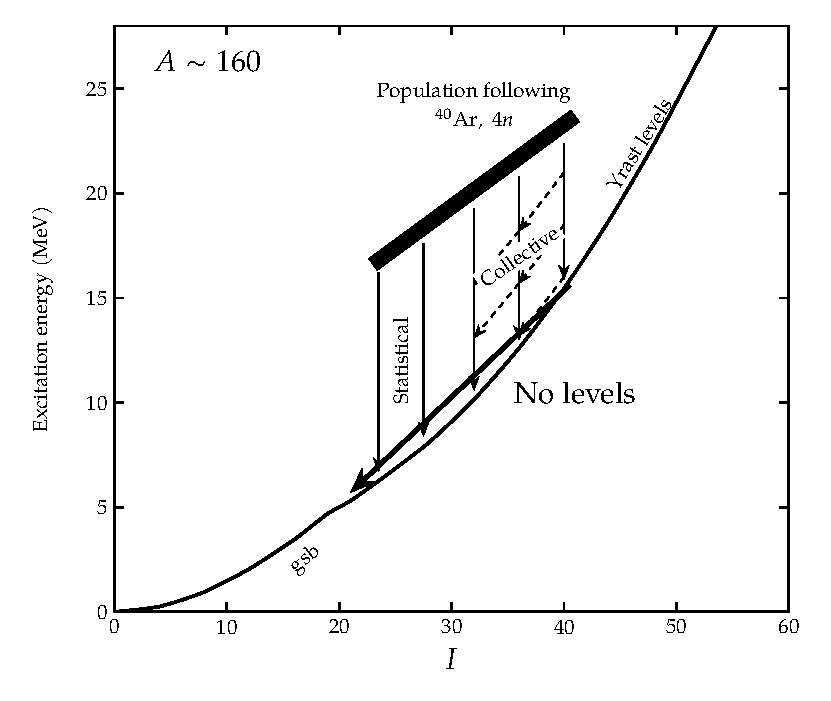
\includegraphics[width=0.7\linewidth]{pictures/3_1}{\small\caption{\label{fig:3.1}{\small 反应($\ce{^{40}Ar},4n$)的激发能-角动量函数关系。在四中子蒸发后，原子核以统计E1和集体E2方式发生$\gamma$级联跃迁，直至晕转线上，而后沿着晕转线发生一系列的E2跃迁。晕转带的强度是逐渐增加的，因为它包含了所有统计跃迁的贡献(\textquotedblleft 边带馈入\textquotedblright )。图片来自文献\cite{SBD77}。}}
} 
\end{figure}

迄今为止，只有这些过程中最后的部分可以被确定为一些分立的线（见3.5节）。通过这种方式所观察到的最大角动量落在$30\hbar$到$40\text{\ensuremath{\hbar}}$之间。目前的测量认为这级联过程的剩余部分是$\gamma$连续的，我们只能从这些实验数据中得到间接的结论{[}GG
67, BSC 75, SBC 76, Di 76, HLM 78, ABH 78, WF 78b{]}。然而，有证据显示沿着平行于晕转线发生的集体跃迁也有着重要的作用；并且在能量高于晕转线几个MeV的地方，集体效应和统计效应存在着竞争{[}SBD
77{]}。

\subsection{晕转带的结构}

在1.7节我们说过一个绕其扁椭球形的对称轴作低角频率转动（Hiskes机制，见图3.2a）下的\emph{经典液滴}\cite{CPS74}。只有在很高的角速度下，原子核会发生相变，并转而由Beringer-Knox机制描述。这种情形下它会发生接近于长椭球形的三轴形变，使得转动轴垂直于其近似的对称轴（见图3.2b）。对于更高的转动频率下，原子核最终会发生衰变（见图3.2c）。

\begin{figure}[H]
\begin{centering}
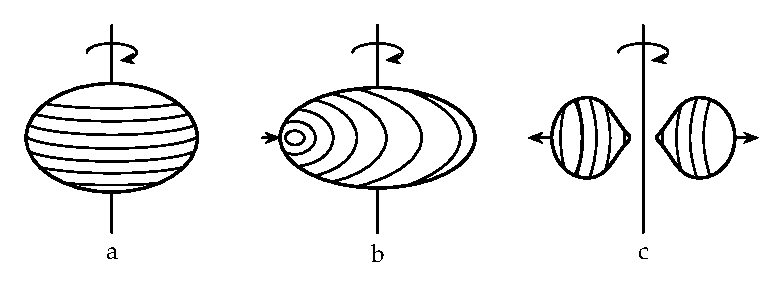
\includegraphics[scale=0.2]{pictures/3_2} 
\par\end{centering}
\caption{\label{fig:3.2}{\small 一个经典液滴在逐渐增长的角速度下的行为}}
\end{figure}

然而，\emph{真实核子}是一个量子力学系统，它表现出壳效应（见2.9节），这使得在元素周期表的某些区域的原子核存在着稳定的基态形变。晕转带对应着每个角动量值的最低能量态；在基态上几十个MeV的激发能全部是转动能量，并且是这些能量产生了角动量。因此，在这条线下的能级密度是很低的，要比在对应能量下$I=0$的能态密度低得多。这个概念类似于基态，然而我们会发现一些对其的典型的偏离。由于核子在晕转区是冷的，我们可以期待其是高度有序的。壳效应起到了重要的作用。

在高角动量下，由壳效应引发的长椭球形变与经典液滴的扁椭球形变具有相同的数量级（见1.7节）。因此当我们研究核子形状与角动量的关系时，我们可以期待在宏观的离心效应与微观的壳结构之间存在的复杂的相互作用。

首先让我们来研究变形良好的重核（例如在稀土区域的元素）的情形。由于壳效应，它们在基态存在着长椭球形的轴对称四极形变。在对应的变形势下，能级由具有相反的单粒子角动量（$\pm\Omega$）的两个核子成对地占领。在第6章我们会看到，就如我们所假设的那样，成对的两个核子不会独立运动，而是由一种配对力耦合在一起——即所谓的自旋为0的Cooper对系统。也就是说，这些形变核会表现出\emph{超流行为}，它们的基态能量也会因此降低几个MeV。

在角动量逐渐增大时，根据晕转带显示出的不同结构，我们可以区分原子核形变的不同机制\cite{BM74}： 
\begin{enumerate}
\item[(a)] 对于较低的角动量量子数$I=0,2,4...$，晕转带与\emph{基态转动带}重合，这在1.5节中已经有过讨论。此时转动是集体的，也就是说转动角速度是与对称轴垂直的（见图3.3a，图中我们已经画出了方向沿着对称轴的Cooper对）。

\begin{figure}[H]
\begin{centering}
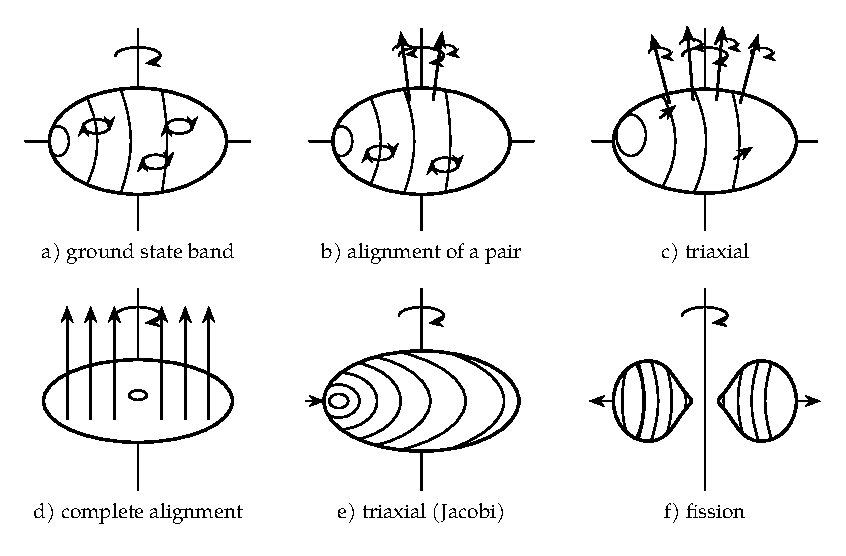
\includegraphics[scale=0.25]{pictures/3_3}\caption{\label{fig:3.3}沿着晕转线形变核的可能结构}
\par\end{centering}
\end{figure}

此时核子处于一个缓慢转动的势场当中（更详细的讨论见3.4节）。对于角动量相反的一对粒子，Coriolis力作用在它们的旋转上，并趋向于让它们的方向与转动轴方向相同，也就是说，Cooper对有被拆开的趋向（\emph{Coriolis拆对效应}；Coriolis
anti-pairing effect, CAP）。然而，在低角动量的情形下，Coriolis力很弱而不足以拆对，原子核将或多或少的与基态时具有相同的结构。

然而我们需要强调的是，在微观图像下，总角动量是由单个核子的角量子数产生的。在集体转动下，这是通过将所有的粒子略微拉向旋转轴方向来实现的。对于每一对粒子而言，这种效应是很小的；粒子对的自旋依然几乎是与势能的对称轴反平行的。当这些小的贡献被累积起来时，我们得到了总角动量$I=2,4...$
\item[(b)] 在角动量逐渐变得越来越大的时候，Coriolis力将变得越来越强，直到大到某一个确定的值时，它将能够拆对。因此在某一个角动量值$I_{c}$时我们可以期待，所有的粒子对都将被拆掉。对关联的消失意味着我们可以观察到一种\emph{相变}，即从超流相向一般相的转变。这种效应在1960年由Mottelson和Valatin所预言\cite{MV60}。
然而更细致的研究表明，Coriolis力的大小是正比于我们所考虑核子的单粒子轨道角动量$j$大小的。在2.8节中我们已经看到，在Fermi面附近的核子分属于不同$j-$值的子壳，而我们期望具有较大$j-$值的那些核子将率先被拉向转动轴的方向。通常，在这样的考虑下，拥有高自旋和相反宇称的能级将在自旋宇称的作用下向下移动，例如稀土元素区的$i_{13/2}$壳层（Stephens-Simon
效应\cite{SS72a}）。

在晕转带的第二种机制之中（见图3.3b），我们可以期待一对或几对已拆对粒子的\emph{顺排过程}，而原子核的其他部分与此同时几乎是不变的。在此之后，晕转带将不再与基态带重合，而是代表着在一个旋转核外存在两个顺排了的粒子体系的能带。两个$i_{13/2}$态的粒子总计能够为转动提供12个单位的角动量。这样的顺排现象的出现是由于，作为集体角速度的函数，角动量$I$的增长是十分迅速的；这会引起能谱上的一些反常效应，例如“回弯现象”（见下）。
\item[(c)] 在平均场的意义上，每一个顺排过程都与集体性质的特定改变联系在一起：被拆的对不再对对关联产生贡献；由于阻塞效应（见6.3.4节），这些关联在若干个顺排过程之后将会完全消失。与旋转轴顺排的粒子的密度分布是一个以旋转轴为对称轴的扁椭球。在与长椭球形的核心结合之后，我们得到了一个三轴形变的混合体。

在晕转带的第三种机制之中（见图3.3c），角动量的大致范围在$30\text{\ensuremath{\lesssim I\lesssim50}}$，我们可以期待Coriolis力与离心力的作用强度能够与壳效应比拟，因此将导致原子核的\emph{三轴形变}。这样的一个没有对称轴的系统要比一个轴对称转子（见1.5.3节）拥有更多的集体态：我们期望存在着平行于晕转带的一系列转动态存在，它们对应着\emph{摆动运动}。
\item[(d)] 如果大多数的核子都与转动轴的方向平行顺排，我们最终得到了一个轴对称的扁椭球。原子核的波函数关于这个轴是转动对称的。转动不再是集体的了；取而代之的是，总角动量是由在变形势阱中不同粒子的重新占据所组成的。

这种运动形式被称为\emph{“单粒子”转动}。在晕转带的这个区域，态的能量是由单粒子能量和转动的扁椭球势阱决定的。相邻态的能量差异会发生统计上的变化。只有在平均意义上，它们符合刚性转子能量的$I(I+1)$定律（见3.4.6节）。从一个态到相邻态的跃迁对应着一次重新占据，并且这矩阵元应该对应着单粒子的值，也就是说这跃迁概率将大幅减少。

由于在晕转带的这个区域能级的统计性特征，我们同时可以期待“高自旋同素异能态”的存在，即所谓的晕阱 \cite{BM74}，这最终会导致延迟衰变的出现，并使我们对整条晕转带级联衰变的观察落在离散的线段上，而不是一个均匀的统计跃迁的背景。
\item[(e)] 在很大角动量的情形下，我们最终期待只有宏观性质是重要的，也就是说，核子应该重复发生扁椭球-三轴-长椭球的形变过程，直至它发生裂变。
\end{enumerate}
迄今为止，只有机制(a)和(b)的离散能级已被观察到；对于剩余区域的很大一部分机制尚处于猜测之中。我们将会在3.4.5节中看到人们曾用以得到这些理论预言的模型。事实上，在计算中我们可以得到上面所讨论的所有机制。

然而，似乎并不是所有原子核都会经历上述的所有阶段。特别是对于小形变或球形核的情况，它们是从机制(d)开始的——也就是说，在发生三轴形变和裂变之前的一个绕着对称轴旋转的扁椭球。另一方面，对于许多大形变的核，在顺排过程中产生的变化不足以补偿其原本长椭球形变所产生的壳效应。在裂变之前它们仅仅会发生三轴形变（见图3.3c与3.3d），而不是扁椭球。在实验上，人们只观测到了作为高自旋同素异能态（晕阱）的小形变原子核，这似乎是与我们的理论符合的。

除了晕转带之外，人们在低自旋和\emph{中自旋区域}观测到了许多其他的转动带。它们的存在基于更加复杂的机制，例如准粒子激发或者是振动态。

在这些机制当中，依赖于$j$壳层轨道的规模，人们可以设想出各种各样的顺排过程。例如在一个奇A核中，在$i_{13/2}$壳上一个奇中子的顺排对应着所谓的\emph{解耦带}。另一个例子是奇奇核中的转动带，此时$i_{13/2}$壳中只有一个中子发生顺排，而质子与对称轴的方向保持一致。这样的带具有一种\emph{半解耦}的结构
\cite{NVR75}。

在3.3节中讨论的粒子加转子模型提供了一种描述这些过程的唯象方法。在那一节中我们将在更细节的程度上讨论以上这些类型的例子。

\subsection{晕转带的唯象描述}

多年来，一些唯象模型被提出来描述转动带的性质和特征。在低自旋区域（见图3.3a），能谱通常符合精确的$I(I+1)$定律；但是对于较大的$I$值，能谱可能发生对这一定律或多或少的偏离\footnote{对于这些数据的一个整合，见 \cite{SHJ73,SSM75}。}。为了描述其与理想的转动谱的偏离，我们通常采取如下的参数化方法：

\begin{equation}
E(I)=A\cdot I\cdot(I+1)+B\cdot(I(I+1))^{2}+C\cdot(I(I+1))^{3}+...
\end{equation}

在很多情况下，这一展开方式的收敛性被证明是相当差的，而一个对\emph{角频率}$\omega$作展开的方法是更合适的。

原则上讲，$\omega$不是一个可以直接测量的量，然而我们可以将其半经典地定义成为

\begin{equation}
\omega=\frac{\text{\ensuremath{\mathrm{d}}}E}{\mathrm{d}J},\text{其中}J=\sqrt{I(I+1)}
\end{equation}

现在将微商用有限差分代替\footnote{这种处理方法不是我们独有的，不同的人会采用不同的处理方法（见\cite{JS74,So73,LR78}）。}，我们可以得到一个“实验”值，\emph{角速度}\footnote{在本章中我们总是使用$\hbar=1$的单位制。}的定义为

\begin{equation}
\omega_{\text{exp}}\simeq\frac{\Delta E}{\Delta\sqrt{I(I+1)}}\bigg|_{I,I-2}\simeq\frac{E(I)-E(I-2)}{\sqrt{I(I+1)}-\sqrt{(I-2)(I-1)}}
\end{equation}

\emph{转动惯量}定义为

\begin{equation}
\mathcal{\mathcal{J}}=\frac{J}{\omega}=\frac{1}{2}\left(\frac{\mathrm{d}E}{\mathrm{d}J^{2}}\right)^{-1}\simeq\frac{2I-1}{\Delta E_{I,I-2}}
\end{equation}

通过这些定义，我们可以计算出晕转带上每一个能级的$\text{\ensuremath{\omega}}$和$\mathcal{J}$的值。
\begin{booknote*}
此时

\[
\mathcal{J}=\frac{J}{\omega}=J\frac{\mathrm{d}J}{\mathrm{d}E}=\frac{1}{2}\left(\frac{\mathrm{d}E}{\mathrm{d}J^{2}}\right)^{-1}
\]
\end{booknote*}
Harris \cite{Ha65a} 提出了如下对能谱的参数化方法：

\begin{equation}
E(I)=\alpha\omega^{2}+\beta\omega^{4}+\gamma\omega^{6}+...
\end{equation}

由于在反向的角速度下，能量$E$不会发生改变，$\omega$的奇数次项不会出现。由于$\omega$是$I$的函数，我们可以选择如(3.3)式中的实验值作为其定义，或者我们也可以定义一个类似上式的转动惯量的展开式，从

\begin{equation}
\frac{\mathrm{d}E}{\mathrm{d}\omega}=\frac{\mathrm{d}E}{\mathrm{d}J}\frac{\mathrm{d}J}{\mathrm{d}\omega}=\omega\frac{\mathrm{d}J}{\mathrm{d}\omega}
\end{equation}

我们可以得到

\[
J(J+1)=\sqrt{I(I+1)}=2\alpha\omega+\frac{4}{3}\beta\omega^{3}+\frac{6}{5}\gamma\omega^{5}+...
\]

当然，这个展开式只有在$J$不是$\omega$的多值函数时才是有效的，也就是说，不在回弯的区域（见3.2.4节）。

另一个被广泛采用来描述转动甚至是过渡性原子核的模型是\emph{可变转动惯量}（variable moment of inertia，VMI）模型
\cite{MSB69,SDG76}。转动惯量$\mathcal{J}$被认为是一个变量，并且有一个内禀的能量$V$依赖于它：

\begin{equation}
E(I,\mathcal{J})=\frac{1}{2\mathcal{J}}I(I+1)+V(\mathcal{J})
\end{equation}

根据变分原理（在5.2中有相关的讨论），对于固定的$I$值，$\mathcal{J}$的取值应该使总能量处于极小值点。这决定了$\mathcal{J}(I)$函数关系。假设我们已知$V(\mathcal{J})$，那么$\mathcal{J}(I)$显然由下式给出

\[
\frac{\mathrm{d}E}{\mathrm{d}\mathcal{J}}\bigg|_{I}=-\frac{1}{\mathcal{J}}\frac{I(I+1)}{2\mathcal{J}}+\frac{\mathrm{d}V}{\mathrm{d}\mathcal{J}}=0
\]

通常我们可以取$V=\frac{1}{2}C(\mathcal{J}-\mathcal{J}_{0})^{2}$，其中$\mathcal{J}_{0}$是在$I=0$处$\mathcal{J}$的取值。系数$C$和$\mathcal{J}_{0}$是从实验能谱$E(I)$拟合得到的。根据关系$J=\omega\cdot\mathcal{J}$，这个模型和Harris模型直至$\omega^{4}$阶是一致的，但(3.7)式的假设显然是更一般的
\cite{DB73,SDG76}。

\subsection{回弯现象}

在10到20个单位角动量的区域，人们在许多核子的晕转带上发现了反常的现象，这现象可以被$\mathcal{J}-\omega^{2}$函数关系图直观地表示出来。在VMI模型的最低阶中（$\mathcal{J}=\mathcal{J}_{0}+b\omega^{2}+...$），这图形应当是一条直线，其对于一个常数的偏离可以作为$I\cdot(I+1)$定律有效性的衡量。图3.4给出了这种曲线的两个例子，由Jülich合作组测得
\cite{LR78}。

\begin{figure}[H]
\centering{}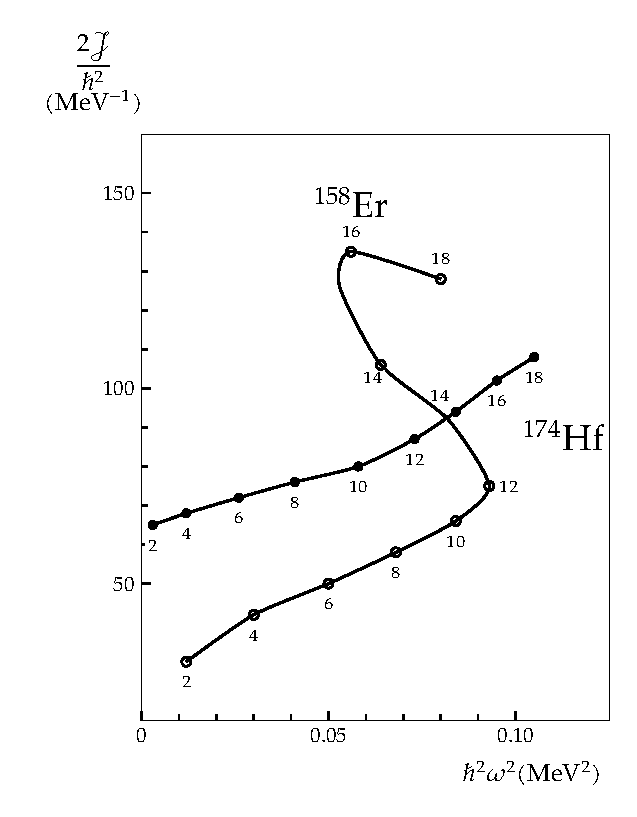
\includegraphics[scale=0.6]{pictures/3_4}\caption{\label{fig:3.4}$^{158}$Er和$^{174}$Hf核的转动惯量-角动量平方的函数图}
\end{figure}

在低自旋的区域我们发现这图形确实是一条直线。对于核$^{174}$Hf，函数对直线的偏离是光滑的。然而对于核$^{158}$Er，在某个特定的$I$值处转动惯量出现了一个都陡峭的上升，甚至使得曲线回弯了（“回弯”现象
\cite{JRH72}）。这在实验上意味着，本应该随着$I$线性增长的跃迁能量$\Delta E_{I,I-2}$

\begin{equation}
\Delta E_{I,I-2}=\frac{1}{2\mathcal{J}}(4I-2)
\end{equation}

不再增大，而是在某一个$I$值开始减小。图3.5给出了与图3.4一致的实验结果。

\begin{figure}[H]
\centering{}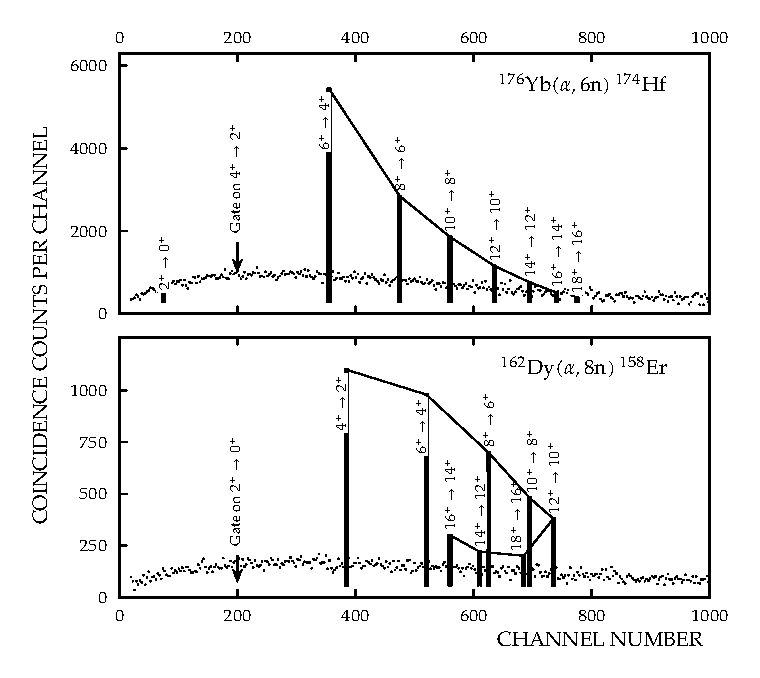
\includegraphics[scale=0.6]{pictures/3_5}\caption{\label{fig:3.5}核反应$^{176}$Yb($\text{\ensuremath{\alpha,6n}}$)$^{174}$Hf和$^{162}$Dy($\text{\ensuremath{\alpha,8n}}$)$^{158}$Er。后一个反应在$I$为$10^{+}-14^{+}$的区域内显示出了名为回弯的反常。为了显示出这种现象，我们用直线将逐渐降低的峰值连接在了一起。}
\end{figure}

这样的现象很容易被两个能带发生交叉的效应所重现（某些情形下我们甚至能够在实验上观测到第二条能带，见图7.6和 \cite{KSM78}）。为了理解这一点，让我们假设两条代表不同转动惯量的曲线在$E-I$图上是两条抛物线。当$\mathcal{J}_{2}>\mathcal{J}_{1}$时，这两条曲线在$I$的某一特定区域会发生交叉。由于剩余相互作用，这样的交叉是不会发生的（不交叉规则，见2.8.4节），因此我们可以得到二阶导数是负的区域，即

\begin{equation}
0>\frac{\mathrm{d}^{2}E}{\mathrm{d}J^{2}}=\frac{\mathrm{d}\omega}{\mathrm{d}J}
\end{equation}

这意味着，随着$\omega$的减小$\mathcal{J}$将变大，同时这两条带的性质将发生交换。事实上，从带混合的观点出发的计算很容易就能解释这样的回弯现象——这样的计算需要包含很少的几个参数，其中一个是两条带之间的相互作用$V$。对于$V$很小的情形，我们会发现一个突兀的转变点，进而发生回弯的现象；而对于$V$较大的情形，转变区域将变得很宽，我们不会再看到回弯现象的出现
\cite{MR72,GG74b}。

\begin{figure}[H]
\centering{}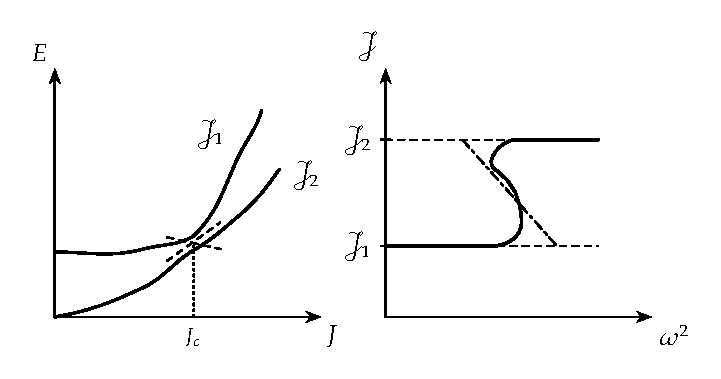
\includegraphics[scale=0.8]{pictures/3_6}\caption{\label{fig:3.6}不同转动惯量曲线$\mathcal{J}_{1}$和$\mathcal{J}_{2}$相互作用的示意图，以及与之对应的回弯现象（取自
\cite{LR78}）}
\end{figure}

另一方面我们很清楚的是，在$\mathcal{J}-\omega^{2}$图形上出现这个奇怪的回弯行为的根源是，我们是在晕转带的一个临界区域探讨问题——我们在背后物理机制不同的两条带之间进行了转换。如果我们只研究基态带的情况，那么对于大$I$值下将不再有晕转带，我们将会得到一条非常平滑的转动惯量关于角速度的曲线（见图3.6中的虚线）。人们经常沿着晕转带研究的原因是其上面的态在实验上是最容易得到的
\begin{comment}
这个问题类似于能级的交叉。对于同一个核，其不同转动机制下的转动惯量曲线很可能存在交叉点，因此使得能量最低的曲线上不止有一种转动惯量的贡献，这种问题似乎可以用最近新出现的本征值延拓方法进行研究——然而对于原本应该交叉之处不交叉的原因，也就是两个“能级”之间的相互作用，暂未有更深层次的理解。此外，能级交叉的现象和相变可能存在着关系。我的理解似乎与下面给出的第一种理论模型相符。
\end{comment}
。

在所有的这些思考之中，我们应该时刻谨记唯象模型只能告诉我们这些能谱的特征，但并不能告诉我们它们背后的物理机制。例如，对于以上讨论的回弯机制，我们可以研究第二条带出现的物理本质。人们已经提出了三种理论解释
\begin{comment}
这三种似乎并非是互斥的；第三种理论解释玄之又玄，我无法理解它描述了怎样的一个物理图像。
\end{comment}
：
\begin{enumerate}
\item 在第二条转动惯量带上，原子核发生了与另一条带不同的形变，例如三轴形变。这意味着回弯现象是由形变的突然改变引起的 \cite{Th73,SV73}。
\item 与基带不同，第二条能带上的状态并不是超流的。这意味着回弯现象是由于从超流体向常规流体相变引发的（Mottelson-Valatin
效应 \cite{MV60}）。
\item 第二条带是由两个绕转动轴转动顺排的准粒子组成的带（见 3.3 节）。此时回弯将对应于一对核子的突然顺排（如 Stephens 和 Simon
所提出 \cite{SS72a}）。
\end{enumerate}
包含所有这些自由度的理论研究（见 7.7 节）的一般结果显示，对于良好形变的核（经典的转子）
\begin{comment}
这里原文直译为“好形变的核”，笔者认为指的应该是形变较为稳定的核。
\end{comment}
，对关联的减少只有在低自旋区会使得转动惯量发生缓慢的增加；但像是回弯一类的突变现象，则是由于一对高 $j$ 轨道核子的顺排而出现的。这种对于回弯现象的解释也有着许多实验上的支持
\cite{GSD73,RSS74,WBB75,SLM76,St76}。

在稀土元素区，$i_{13/2}$ 的中子扮演着重要的角色。然而实验上 \cite{LAD77,BBB79a} 在自旋为 $26\sim30\,\hbar$
\begin{comment}
原文如此，令人怀疑角动量的单位。
\end{comment}
的区域发现了第二个反常现象存在的证据，即所谓的\emph{二次回弯}。这一现象被解释为一对 $h_{11/2}$ 质子的顺排 \cite{FP78}。其他高
$j$ 轨道的核子可能在周期表其他区域的元素中扮演着类似的角色。
\begin{comment}
终此一节，我们在研究唯象模型的解释时将“alignment”译为对齐，在含义上指的是一对核子自旋轴变为了平行方向；然而此译法似不常用。
\end{comment}


\section{粒子加转子模型}

为了描述粒子运动和集体转动之间的相互关系，Bohr 和 Mottelson \cite{BM53} 提出了一个模型：考虑若干近似独立地运动于核心形变势阱中的价粒子，并将它们与一个代表其余粒子的集体转子相耦合。划分价粒子和核心的方式并不总是唯一的。然而一种合理的方式是，在奇
$A$ 核中将未成对的核子视为价核子，而留下一个偶偶核心。我们也可以将粒子-空穴激发的粒子和空穴视为价粒子
\begin{comment}
这里类似壳模型，只不过处理的Hamilton量不太一样。
\end{comment}
。更一般地来讲，我们可以将 Hamilton 量分为两部分：内禀部分 $H_{\text{intr}}$，其在微观层面上描述价粒子或
Fermi 面附近的一整组核子；以及一个用来描述惰性核心的唯象部分 $H_{\text{coll}}$：

\begin{equation}
H=H_{\text{intr}}+H_{\text{coll}}\label{eq:3.10}
\end{equation}

\emph{内禀部分}具有如下形式：

\begin{equation}
H_{\text{intr}}=\sum_{k}\epsilon_{k}a^{\dagger}_{k}a_{k}+\frac{1}{4}\sum_{klmn}\bar{v}_{klmn}a^{\dagger}_{k}a^{\dagger}_{l}a_{n}a_{m}\label{eq:3.11}
\end{equation}

此处 $\epsilon_{k}$ 是形变势中的单粒子能量（例如 Nilsson 能量），而 $\bar{v}$ 是价粒子间的相互作用——在很多情况下这是可以被忽略的。\footnote{我们将在第6章中看到，对关联在形变核中起着重要作用，因此我们应当讨论准粒子而非粒子。这仅给下面给出的公式带来简单的占据因子，出于完整性考虑我们有时会给出这些因子。如欲深入理解，读者可参阅第6章。}

\textit{集体的部分}描述了惰性核心的转动：

\begin{equation}
H_{\text{coll}}=\frac{R^{2}_{1}}{2\mathcal{J}_{1}}+\frac{R^{2}_{2}}{2\mathcal{J}_{2}}+\frac{R^{2}_{3}}{2\mathcal{J}_{3}}\label{eq:3.12}
\end{equation}
其中 $R_{i}$ 是核心集体角动量在体固坐标系中的分量。它与价粒子的角动量 $\boldsymbol{j}$（即各单粒子角动量之和）共同构成了总角动量
$\boldsymbol{I}$（参见附录 A）：

\begin{equation}
\boldsymbol{I}=\boldsymbol{R}+\boldsymbol{j}\label{eq:3.13}
\end{equation}
消去 $\boldsymbol{R}$ 后，$H_{\text{coll}}$ 可以分解为三部分：

\begin{equation}
H_{\text{coll}}=H_{\text{rot}}+H_{\text{rec}}+H_{\text{cor}}\label{eq:3.14}
\end{equation}
其中

\begin{equation}
H_{\text{rot}}=\frac{I^{2}_{1}}{2\mathcal{J}_{1}}+\frac{I^{2}_{2}}{2\mathcal{J}_{2}}+\frac{I^{2}_{3}}{2\mathcal{J}_{3}}\label{eq:3.15}
\end{equation}
是转子的纯转动算符{[}式 (1.55){]}，它仅作用于转子的自由度，即 Euler 角。项

\begin{equation}
H_{\text{rec}}=\sum^{3}_{i=1}\frac{j^{2}_{i}}{2\mathcal{J}_{i}}\label{eq:3.16}
\end{equation}
通常被称为\emph{反冲项}（recoil term）。它代表转子的反冲能量。该算符仅作用于价粒子的坐标空间。对于多个价粒子的情形，它包含两体相互作用。

最后，Coriolis 相互作用

\begin{equation}
H_{\text{cor}}=-\sum^{3}_{i=1}\frac{I_{i}j_{i}}{\mathcal{J}_{i}}\label{eq:3.17}
\end{equation}
将价粒子的自由度与转子的自由度耦合在一起。这种纯粹的运动学耦合是该模型中唯一的耦合作用。

应当注意到，实验室坐标系中的总角动量算符 $I_{x},I_{y},I_{z}$ 与 Hamilton 量 \ref{eq:3.10}
对易。尽管在内禀参考系中转动对称性受到了破坏（例如在 Nilsson Hamilton 量中），但该模型对于全系统仍然保持角动量守恒，这是因为算符
$I_{x},I_{y},I_{z}$ 仅作用于 Euler 角，并与内禀分量 $I_{1},I_{2},I_{3}$ 对易（参见附录
A）。然而必须强调的是，这种转动不变性仅仅是通过引入唯象的核心才得以实现的。如果人们希望微观地处理所有粒子（即核心消失的极限），Euler
角就成了冗余变量（参见 11.3 节）。

系统的波函数可以写为

\begin{equation}
|\Psi^{I}_{M}\rangle=\sum_{K}\Phi_{K}|IMK\rangle\label{eq:3.18}
\end{equation}
其中 $\Phi_{K}$ 依赖于价粒子的坐标，而 $|IMK\rangle$ 依赖于 Euler 角，并在式 (A.21) 中定义。在最简单的特定情形下，体系仅包含一个价粒子与一个轴对称转子。利用该模型，人们极其精确地重现了奇
$A$ 核的大量实验能谱；从这一角度来看，它无疑是核物理中最有力的模型之一。然而，迄今为止该模型仍缺乏严密的微观推导。这样一个推导应当从多体
Hamilton 量 (2.19) 出发，将 $3A$ 个粒子坐标以适宜的方式变换为 $3A-3$ 个内部坐标以及描述集体运动的
3 个 Euler 角。与该变换相对应，Hamilton 量应分解为内部部分与集体部分，正如\ref{eq:3.10} 所示。最终，人们希望利用形变壳模型来描述内部运动。

人们在这一方向上做出了许多尝试，我们在 11.3 节中对此给出了简要讨论，但直到目前该问题仍未得到彻底解决。对于良好形变核的情形，该模型可以由以下论据提供支持：
\begin{enumerate}
\item[(i)] 微观 Hartree-Fock 计算在轴对称形变处展现出非常显著的能量极小值，这证实了转动核心概念的合理性。
\item[(ii)] 该模型在一定程度上等价于 cranking 模型（参见 3.4 节），后者至少在强轴对称形变极限下具有微观基础。
\item[(iii)] Villars 和 Cooper \cite{VC70} 证明，在引入冗余坐标后，可以得到类似于\ref{eq:3.10} 形式的
Hamilton 量，不过带有额外的耦合项。在强形变极限并引入进一步假设的前提下，他们得到了正确的转动惯量表达式。
\end{enumerate}
然而，粒子加转子模型也被非常成功地应用于小形变区以及过渡核中。目前尚不清楚这一成功如何从微观上予以解释。

\subsection{轴对称情形}

假设转子以 3 轴为对称轴，即 $\mathcal{J}_{1}=\mathcal{J}_{2}=\mathcal{J}$，此时不可能存在绕该轴的集体转动，因而
$\boldsymbol{R}$ 的 3 分量必须为零（参见 1.5 节）。由\ref{eq:3.13} 立即得到，总角动量 $\boldsymbol{I}$
的 3 分量 $K$ 必定等于 $\boldsymbol{j}$ 的 3 分量 $\Omega$：

\begin{equation}
K=\Omega\label{eq:3.19}
\end{equation}
对于 Hamilton 量 \ref{eq:3.10}、\ref{eq:3.14} 中的各项，在此情形下我们得到：

\begin{equation}
H_{\text{intr}}=\sum_{i,\Omega}\epsilon^{i}_{\Omega}a^{\dagger}_{i\Omega}a_{i\Omega}\label{eq:3.20}
\end{equation}

\begin{equation}
H_{\text{rot}}=\frac{\boldsymbol{I}^{2}-I^{2}_{3}}{2\mathcal{J}}\label{eq:3.21}
\end{equation}

\begin{equation}
H_{\text{rec}}=\frac{1}{2\mathcal{J}}\left(j^{2}_{1}+j^{2}_{2}\right)\label{eq:3.22}
\end{equation}

\begin{equation}
H_{\text{cor}}=-\frac{1}{\mathcal{J}}\left(I_{1}j_{1}+I_{2}j_{2}\right)=-\frac{1}{2\mathcal{J}}\left(I_{+}j_{-}+I_{-}j_{+}\right)\label{eq:3.23}
\end{equation}
在\ref{eq:3.20} 中我们忽略了剩余相互作用。轴对称势阱中的单粒子能级由量子数 $k=(i,\Omega)$ 标记，对应的本征函数记为
$\Phi^{i}_{K}$。

反冲项仅作用于内禀坐标。它经常被忽略，因为内禀单粒子能量 $\epsilon^{i}_{\Omega}$ 通常是根据实验数据进行拟合调节的。在接下来的讨论中我们遵循这一论据，暂且略去
$H_{\text{rec}}$。直到 3.3.2.1 节我们才会重新讨论它。Hamilton 量 \ref{eq:3.20}–\ref{eq:3.23}
具有\ref{eq:3.18} 类型的本征函数，这可以通过对 Hamilton 量 \ref{eq:3.10} 进行数值对角化求得。然而，\ref{eq:3.20}–\ref{eq:3.23}
中各项的重要性取决于具体的物理情境。因此，考察以下三种极限是非常有益的；在这些极限中某一项占据主导地位，从而使问题能够解析求解（综述参见
\cite{St75a}）：

在\emph{强耦合极限}下，奇粒子绝热地跟随偶偶核心的转动。当与形变的耦合远强于 Coriolis 相互作用对单粒子运动的微扰时，该极限得以实现。

在\emph{弱耦合极限}下（对应于极小的形变），奇粒子基本上运动于球形壳模型能级上，仅受到微弱的扰动（例如来自四极振动的扰动，参见第
8 章）。

在\emph{解耦极限}下，Coriolis 力非常强烈，以至于与核心形变的耦合可以忽略。此时总角动量与单粒子角动量彼此平行。

\subsubsection{强耦合极限（形变顺排）}

当 Coriolis 相互作用矩阵元与形变壳模型中不同 $\Omega$ 值的单粒子能量能级分裂相比非常微小时，强耦合极限得以实现。我们预期在以下情况下满足该条件：
\begin{enumerate}
\item[(i)] 大形变 $\beta$ 的情形，因为 Nilsson Hamilton 量中的能级分裂正比于 $\beta$，而根据简易经验规则{[}式
(1.50){]}，转动常数 $\hbar^{2}/(2\mathcal{J})\propto\beta^{-2}$；
\item[(ii)] Coriolis 矩阵元很小的微扰情形。正如我们在\ref{eq:3.33} 中将看到的，它们正比于 $[I(I+1)-K(K+1)]^{1/2}[j(j+1)-\Omega(\Omega+1)]^{1/2}$，这意味着在低自旋
$I$ 或处于小粒子角动量 $j$ 轨道的核子情况下该矩阵元很小。对于大的 $j$ 值，只有在很大的 $\Omega$ 值下它们才可以被忽略。
\end{enumerate}
这一极限被称为强耦合或\emph{形变顺排}（deformation aligned）极限，因为在这种情况下 $K$ 是一个好量子数。价粒子的角动量
$\boldsymbol{j}$ 强烈耦合到核心的运动上。在半经典图像中，$\boldsymbol{j}$ 绕 3 轴进动，如\ref{fig:3.7}a
的耦合方案所示。由于 $H_{\text{cor}}$ 是 Hamilton 量中耦合粒子与转子自由度的唯一项，在这一极限下本征函数是函数
$\Phi_{K}$（$H_{\text{intr}}$ 的本征函数，例如单粒子 Nilsson 函数）与对称转子本征函数 $|IMK\rangle$
的直积（参见附录 A）。

\begin{figure}[H]
\begin{centering}
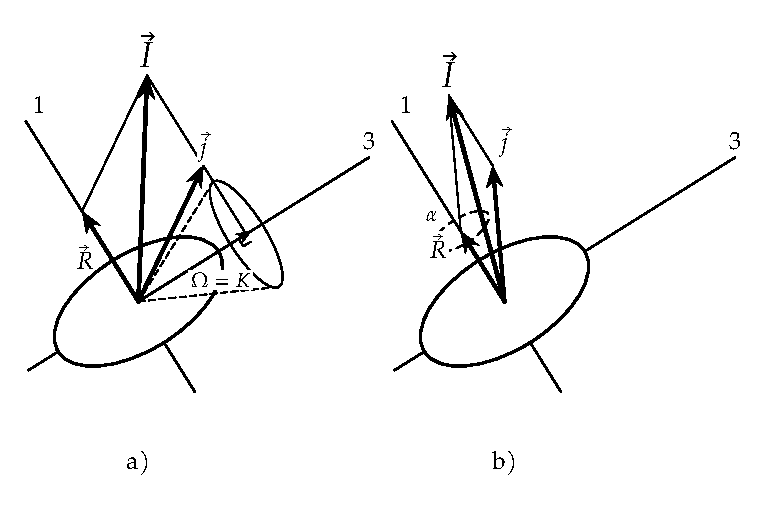
\includegraphics[width=0.7\textwidth]{pictures/3_7}
\par\end{centering}
\caption{\label{fig:3.7}粒子加转子模型中的耦合方案：(a) 强耦合；(b) 转动顺排。}
\end{figure}

我们在 1.5.1 节中已经看到，Hamilton 量 \ref{eq:3.10} 具有额外的对称性 $\mathcal{R}_{1}$，它描述了核心绕体固坐标系
1 轴转动 $180^{\circ}$ 的操作：

\begin{equation}
\mathcal{R}_{1}=\mathrm{e}^{\mathrm{i}\pi R_{1}}=\mathrm{e}^{\mathrm{i}\pi I_{1}}\mathrm{e}^{-\mathrm{i}\pi j_{1}}\label{eq:3.24}
\end{equation}
因此我们必须对波函数 \ref{eq:3.18} 进行对称化，结合式 (A.24) 得到如下本征函数集合 \cite{Ke56}：

\begin{equation}
|\Psi^{I}_{MK}\rangle=\frac{1}{\sqrt{2(1+\delta_{K0})}}\left\{ \Phi^{i}_{K}|IMK\rangle+(-)^{I}\mathrm{e}^{-\mathrm{i}\pi j_{1}}\Phi^{i}_{K}|IM-K\rangle\right\} \label{eq:3.25}
\end{equation}
如果我们已知 $\Phi^{i}_{K}$ 在 $\boldsymbol{j}^{2}$ 本征态上的展开：

\begin{equation}
|\Phi^{i}_{K=\Omega}\rangle=\sum_{nj}C^{i}_{nj}|nj\Omega\rangle\label{eq:3.26}
\end{equation}
我们便发现

\begin{equation}
\mathrm{e}^{-\mathrm{i}\pi j_{1}}|\Phi^{i}_{K=\Omega}\rangle=\sum_{nj}C^{i}_{nj}(-)^{-j}|nj-\Omega\rangle\label{eq:3.27}
\end{equation}
与\ref{eq:3.25} 相对应的能谱由下式给出：

\begin{equation}
E^{i}_{K}(I)=\epsilon^{i}_{K}+\frac{1}{2\mathcal{J}}\left(I(I+1)-K^{2}\right)\label{eq:3.28}
\end{equation}
{[}在\ref{eq:3.28} 中，通常用准粒子能量 $E^{i}_{K}$ 代替 $\epsilon^{i}_{K}$，其定义见式
(6.72){]}。这是转动带的能谱。最低可能的自旋为 $I_{0}=K$。带头能量 $E^{i}_{K}(I_{0})$ 并不严格等于
$\epsilon^{i}_{K}$，而是有微小的位移，尤其是当我们计入反冲项与剩余相互作用时。该能谱具有能级间距 $\Delta I=1$，其转动惯量即为转子的转动惯量。

在这一强耦合极限下，我们完全忽略了 Coriolis 相互作用。若至少在一阶微扰论下计入它，我们仅在 $K=1/2$ 的能带中获得修正：

\begin{equation}
E^{i}_{K=1/2}(I)=\epsilon^{i}_{K=1/2}+\frac{1}{2\mathcal{J}}\left\{ I(I+1)-\frac{1}{4}+a^{i}\left(I+\frac{1}{2}\right)(-)^{I+1/2}\right\} \label{eq:3.29}
\end{equation}
其中所谓的\emph{解耦因子}（decoupling factor）由下式给出：

\begin{equation}
a^{i}=\mathrm{i}\langle\Phi^{i}_{1/2}|j_{+}\mathrm{e}^{-\mathrm{i}\pi j_{1}}|\Phi^{i}_{1/2}\rangle\label{eq:3.30}
\end{equation}
或者若 $\Phi^{i}_{K}$ 具有\ref{eq:3.26} 的形式：

\begin{equation}
a^{i}=-\sum_{nj}|C^{i}_{nj}|^{2}(-)^{j+1/2}\left(j+\frac{1}{2}\right)\label{eq:3.31}
\end{equation}
这意味着，例如对于正的解耦因子（主要成分具有半整数 $j+\frac{1}{2}$ 为奇数），具有 $I+\frac{1}{2}$
为奇数的能级（$I=\frac{1}{2},\frac{5}{2},\frac{9}{2},\dots$）向下移动。这极好地解释了许多核中
$K=1/2$ 能带出现的相当严重的交错扭曲现象 \cite{ABH56}；事实上在这些核中，具有 $\Delta I=2$
的两条分支带（$I+\frac{1}{2}$ 的偶数与奇数值）彼此相对位移。导致这种解耦的原因来自波函数关于 $\mathcal{R}_{1}$
对称化的\ref{eq:3.25}，它通过 Coriolis 矩阵元混合了 $K=1/2$ 与 $K=-1/2$ 的态。解耦因子
$a^{i}$ 的强度取决于对单粒子波函数 $\Phi^{i}_{1/2}$ 有贡献的 $j$ 分量。如果涉及具有大单粒子角动量的能级，解耦因子将非常巨大。然而在这些情况下微扰论不再成立，Coriolis
算符的其他矩阵元也会参与进来。因此，强耦合极限不再能实现，我们必须考虑不同的极限情形。

\subsubsection{弱耦合极限（无顺排）}

如前所述，当 Coriolis 矩阵元在属于不同 $K$ 值的单粒子能级之间引起强混合时，强耦合近似便失效了。因此让我们更详细地研究
Coriolis 矩阵元：

\begin{equation}
\langle\Psi^{I}_{MK+1}|H_{\text{cor}}|\Psi^{I}_{MK}\rangle=-\frac{1}{\mathcal{J}}\sqrt{I(I+1)-K(K+1)}\,\langle\Phi_{\Omega+1}|j_{x}|\Phi_{\Omega}\rangle\label{eq:3.32}
\end{equation}
若 $\Phi_{\Omega}$ 具有\ref{eq:3.26} 所示的形式，我们得到

\begin{equation}
\langle\Psi^{I}_{MK+1}|H_{\text{cor}}|\Psi^{I}_{MK}\rangle=-\frac{1}{2\mathcal{J}}\sum_{nj}|C_{nj}|^{2}\sqrt{I(I+1)-K(K+1)}\sqrt{j(j+1)-\Omega(\Omega+1)}\label{eq:3.33}
\end{equation}
我们看到，当 $I/K$ 与 $j/\Omega$ 很大时，这些矩阵元非常大。也就是说，当涉及具有大 $j$ 与小 $\Omega$
值的能级时便属于此情形。处于这些能级中的粒子具有高角动量，其密度分布紧贴 3 轴。因此显而易见，核心垂直于该轴的转动会对这些粒子的运动产生巨大的影响。

一个著名的例子是中子 $1i_{13/2}$ 能级，在轻稀土核（如 Dy 和 Er）中它位于 Fermi 面附近。人们可以估计在
$\Omega=1/2$ 情形下 Coriolis 矩阵元约为 $0.1\times I\,\text{MeV}$，与 $H_{\text{intr}}$
的能级间距相比这实际上是相当大的。由于这些具有高 $j$ 值的能级被壳模型的自旋-轨道耦合项（参见 2.4 节）极大地向下压入具有不同主量子数
$N$ 的壳层中，这些能级具有相当纯的组态，即 $C_{nj}\simeq1$（闯入态，intruder state）。因此在接下来的讨论中，仅考虑这样一个单独的
$j$ 壳层就足够了。$1i_{13/2}$ 壳层并不是唯一的特例。每个主壳层中具有最大 $j$ 值的能级能量都被急剧拉低，并在许多转动能谱中扮演着极其重要的角色。

Vogel \cite{Vo70} 提出了一个极限（通常称为\emph{弱耦合}或\emph{无顺排}极限），其中 $H_{\text{intr}}$
的 $K$ 分裂被完全忽略。（当然，这只有在极小形变下才是有效的近似。）此时 $\boldsymbol{j}^{2}$ 与 $\boldsymbol{R}^{2}$
均与 $H_{\text{intr}}$ 对易，我们可以构造 $\boldsymbol{R}^{2}$ 与 $R_{3}$ 的共同本征函数（后者的本征值自然为零）。适当的角动量耦合给出\footnote{由于我们将角动量 $\boldsymbol{j}$ 与 $-\boldsymbol{I}$ 耦合为 $\boldsymbol{R}=\boldsymbol{I}-\boldsymbol{j}$，我们必须采用反相位的耦合规则，参见附录
A。}：

\begin{equation}
|\Psi^{IR}_{M}\rangle=\sum_{K}(-)^{j-K}C^{I\quad j\quad R}_{K\ -K\ 0}\Phi_{K}|IMK\rangle\label{eq:3.34}
\end{equation}
这些波函数对角化了 $\boldsymbol{R}^{2}$，对应的能谱形式为

\begin{equation}
E(I)=E_{\text{intr}}+\frac{1}{2\mathcal{J}}R(R+1)\label{eq:3.35}
\end{equation}
满足

\begin{equation}
|j-R|\leqslant I\leqslant j+R;\quad R=0,2,4,\dots\quad(\mathcal{R}_{1}\ \text{对称性})\label{eq:3.36}
\end{equation}
这意味着对于转子的每一个转动量子数 $R$，$\boldsymbol{j}$ 可以有 $2j+1$ 种不同的空间取向而不改变系统的能量（零耦合）。这
$2j+1$ 个能级的分裂可以在一阶微扰论下予以考虑（我们采用 Nilsson 项 $\sim\beta r^{2}Y_{20}$
作为微扰）：

\begin{equation}
E(I)=E_{0}+\frac{1}{2\mathcal{J}}R(R+1)-\beta\hbar\omega_{0}\langle\Psi^{IR}_{M}|r^{2}Y_{20}|\Psi^{IR}_{M}\rangle\label{eq:3.37}
\end{equation}
对应于 $\boldsymbol{j}$ 的每一种取向，都存在核心的一整条具有 $\Delta R=2$ 的转动带。在给定的能量下（即给定的
$R$），具有最高 $I$ 值的能级 $I=R+j$ 对应于晕能级（yrast levels）。这些能级之间由强 $E2$
跃迁相连接 \cite{Re75a}，并在实验上最容易被观测到。它们被称为\emph{优选态}（favored states）\footnote{具有较低顺排程度的能级（例如 $I=j+R-1$）被称为非优选态（unfavored states）。}
\cite{St75a}，其能量由下式给出：

\begin{equation}
E(I)=E_{\text{intr}}+\frac{1}{2\mathcal{J}}(I-j)(I-j+1)\label{eq:3.38}
\end{equation}
这意味着这些态位于一条在 $I=j$ 处具有极小值的抛物线上，这在实验上得到了广泛的证实，\ref{fig:3.8} 给出了一个典型范例。

\begin{figure}[H]
\begin{centering}
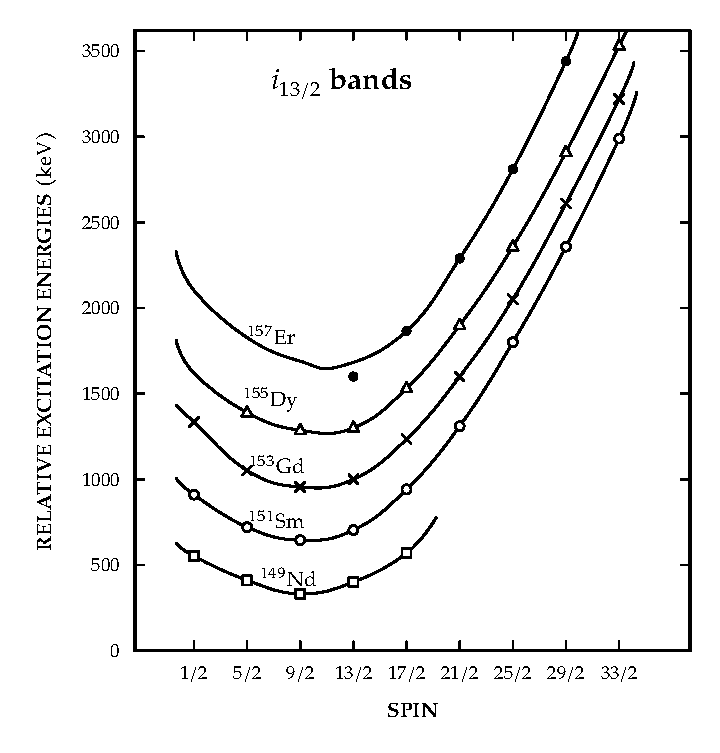
\includegraphics[width=0.75\textwidth]{pictures/3_8}
\par\end{centering}
\caption{\label{fig:3.8}某些 $N=89$ 核中 $1i_{13/2}$ 带的相对激发能随自旋的变化关系。（实验观测到的能带成员在绘制时将
$13/2^{+}$ 态等间距平移（300 keV）。引自 \cite{LR76}。）}
\end{figure}

在这条抛物线的右支上，$\boldsymbol{j}$ 与 $\boldsymbol{R}$ 相互顺排（$\boldsymbol{j}\parallel\boldsymbol{R}$）：

\[
I=j+R=j,j+2,j+4,\dots
\]
而在抛物线的左支上，$\boldsymbol{j}$ 与 $\boldsymbol{R}$ 反向顺排（$\boldsymbol{j}\parallel-\boldsymbol{R}$）；核心的转动方向与
$\boldsymbol{j}$ 相反\footnote{原则上也存在具有 $R>j$ 的反向顺排态 \cite{PO78}。}：

\[
I=j-R=j-2,j-4,\dots,\frac{1}{2}\left(\text{或 }0\right)
\]
作为一条经验规则，弱耦合极限严格来说仅在非常小的形变 $|\beta A^{1/3}|<4$ 下才成立。然而我们将在下一小节看到，即使在更强的形变下（此时忽略
$H_{\text{intr}}$ 的 $\Omega$ 依赖性已不再合理），满足 $\boldsymbol{I}\parallel\boldsymbol{j}$
的态在能量上仍然是极其有利的。因此，在所谓转动顺排耦合方案中，\ref{eq:3.38} 对于更大形变核中的许多能级同样适用（例如参见\ref{fig:3.8}）。

\subsubsection{解耦极限（转动顺排）}

在处于中等形变的情形下，Hamilton 量内禀部分的能级分裂不再能够被忽略。此时外层大 $j$ 粒子的取向不再独立于核心的运动。Stephens
等人 \cite{SDN73} 认识到，若外层粒子沿着长椭球核的转动轴顺排，则单粒子密度分布（主要集中在垂直于 $\boldsymbol{j}$
的平面内）与核心之间的最大重叠要求便能够得到满足（参见 2.8.4 节）。

在数学上，我们可以在单一 $j$ 壳层模型中理解这一点（$C_{nj}\simeq1$，例如在 $1i_{13/2}$ 情形下）。忽略
$\boldsymbol{l}^{2}$ 与 $\boldsymbol{l}\cdot\boldsymbol{s}$ 项，Nilsson
能量简单地由对角矩阵元给出：

\begin{align}
\epsilon_{\Omega} & =\epsilon_{0}-\beta\hbar\omega_{0}\langle nlj\Omega|r^{2}Y_{20}|nlj\Omega\rangle\nonumber \\
 & =\epsilon_{0}+\beta k\frac{3\Omega^{2}-j(j+1)}{4j(j+1)}=\epsilon_{0}-\frac{1}{4}\beta k+C\Omega^{2}\label{eq:3.39}
\end{align}
其中 $k$ 与 $C$ 均不依赖于 $\Omega$。同样，反冲项 \ref{eq:3.22} 可以作为对角矩阵元计算，给出

\begin{equation}
H_{\text{rec}}=\frac{1}{2\mathcal{J}}\left(j(j+1)-\Omega^{2}\right)\label{eq:3.40}
\end{equation}
因此，在此近似下 Hamilton 量 \ref{eq:3.10} 具有形式：

\begin{equation}
H=\epsilon_{0}-\frac{1}{4}\beta k+\frac{1}{2\mathcal{J}}\left(I(I+1)+j(j+1)\right)+\left(C-\frac{1}{2\mathcal{J}}\right)\Omega^{2}+H_{\text{cor}}\label{eq:3.41}
\end{equation}
在特定的形变区域，当 $C\simeq1/(2\mathcal{J})$ 时，来自 Hamilton 量内禀部分与转动部分的 $\Omega$
依赖性恰好相互抵消！事实证明，这一相消对于相当宽广的中等形变区域都适用。遗憾的是，求解\ref{eq:3.41} 所需的 $H_{\text{cor}}$
的本征函数在一般情形下无法解析给出。因此我们在此给出定性的讨论。将 Coriolis 项写作\footnote{$\boldsymbol{I}_{\perp}$ 与 $\boldsymbol{j}_{\perp}$ 分别是 $\boldsymbol{I}$
与 $\boldsymbol{j}$ 垂直于对称轴的分量。}：

\begin{equation}
H_{\text{cor}}=-\frac{1}{\mathcal{J}}\boldsymbol{I}_{\perp}\cdot\boldsymbol{j}_{\perp}\label{eq:3.42}
\end{equation}
我们看到，对于满足 $\langle\boldsymbol{I}\rangle\parallel\langle\boldsymbol{j}\rangle$
的波函数，它的期望值最低。由于 $\boldsymbol{R}$ 垂直于 3 轴，对于单粒子角动量沿垂直于对称轴的转动轴顺排的波函数，我们获得最低的本征值。为此，我们选取
1 轴，并相应地通过将 $j_{3}$ 的本征函数 $|\Phi^{j}_{K}\rangle$ 绕 2 轴旋转 $90^{\circ}$，构造具有本征值
$\alpha$ 的 $j_{1}$ 的本征函数 $|\tilde{\Phi}_{\alpha}\rangle$：

\begin{equation}
|\tilde{\Phi}_{\alpha}\rangle=\sum_{K}d^{j}_{K\alpha}\left(-\frac{\pi}{2}\right)|\Phi^{j}_{K}\rangle\label{eq:3.43}
\end{equation}
其中 $d^{j}_{K\alpha}$ 是该转动的 Wigner 函数 \cite{Ed57}。

然而对于总波函数而言，构造使 $\alpha$ 成为好量子数的态并不那么容易。尝试波函数

\begin{equation}
|\Psi^{I\ j}_{M\ \alpha}\rangle=\sum_{K}d^{j}_{K\alpha}\left(-\frac{\pi}{2}\right)\Phi^{j}_{K}|IMK\rangle\label{eq:3.44}
\end{equation}
至少在 $I\gg K$ 时是 $H_{\text{cor}}$ 的本征函数。由

\begin{equation}
I_{-}|IMK\rangle=\sqrt{I(I+1)-K(K+1)}|IMK+1\rangle\simeq I|IMK+1\rangle\label{eq:3.45}
\end{equation}
我们随即容易得到

\begin{equation}
H_{\text{cor}}|\Psi^{I\ j}_{M\ \alpha}\rangle=-\frac{1}{\mathcal{J}}I\alpha|\Psi^{I\ j}_{M\ \alpha}\rangle\quad(I\gg K)\label{eq:3.46}
\end{equation}
这表明 $\alpha$ 即为 $\boldsymbol{j}$ 在 $\boldsymbol{I}$ 上的投影。

由式 (A.24) 以及 \cite[式 (4.2.4)]{Ed57}，我们得到

\begin{equation}
\mathcal{R}_{1}|\Psi^{I\ j}_{M\ \alpha}\rangle=(-)^{I-\alpha}|\Psi^{I\ j}_{M\ \alpha}\rangle\label{eq:3.47}
\end{equation}
这意味着为了满足对称性条件 $\mathcal{R}_{1}=1$，$I-\alpha$ 必须为偶数。

在 $C\simeq1/(2\mathcal{J})$ 的情形下，对于 Hamilton 量 \ref{eq:3.41} 的能谱我们发现：

\begin{align}
E(I,\alpha) & =\text{const.}+\frac{1}{2\mathcal{J}}\left(I(I+1)+j(j+1)-2I\alpha\right)\nonumber \\
 & =\text{const.}+\frac{1}{2\mathcal{J}}(I-\alpha)(I-\alpha+1)\label{eq:3.48}\\
 & =\text{const.}+\frac{1}{2\mathcal{J}}R(R+1)\label{eq:3.49}
\end{align}
其中根据对称性条件 \ref{eq:3.47}，$R=I-\alpha=0,2,4,\dots$ 必须为偶数。

因此，能量最低的态是那些具有最大顺排的态（$\alpha=j$，优选态）。这完全对应于价核子的自旋取向垂直于 3 轴、而核心完全解耦并以
$R=I-\alpha$ 转动的物理图像；它给出了间距为 $\Delta I=2$ 的能谱，但在其他方面与邻近偶偶核的转动谱完全等价。例如在弱形变核中已经观测到了这类能带（参见\ref{fig:3.8}
与\ref{fig:3.9}）。

\begin{figure}[H]
\begin{centering}
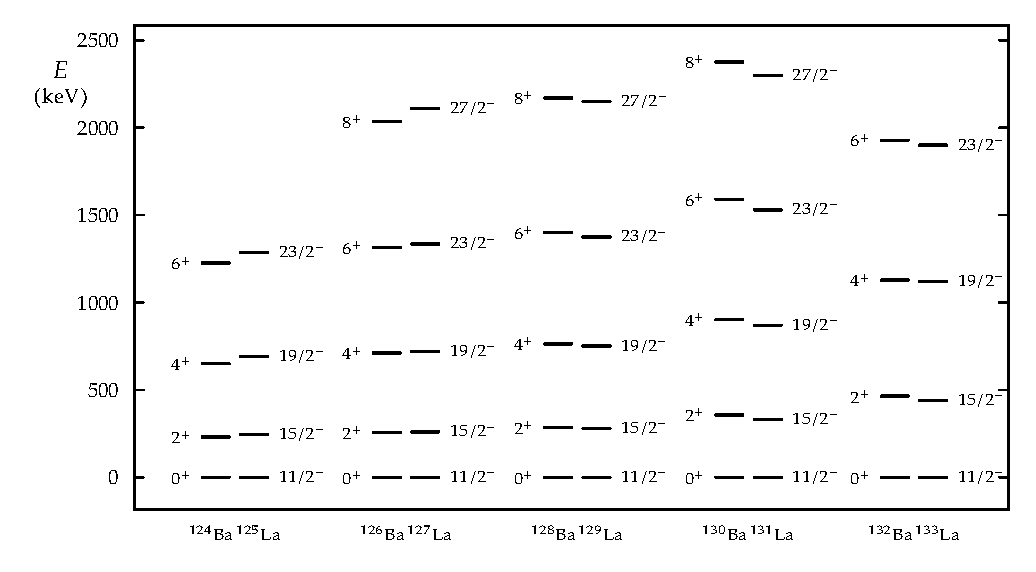
\includegraphics[width=0.75\textwidth]{pictures/3_9}
\par\end{centering}
\caption{\label{fig:3.9}某些 Ba 同位素中的基带能级与邻近 La 核中负宇称带能级的比较。在大多数情况下，La 的 $11/2^{-}$
能级并非基态，其能量已从该核展示的所有能级中扣除。（引自 \cite{St75a}。）}
\end{figure}

顺排程度较低的态（非优选态）具有 $\alpha=j-1$。它们通常位于更高的能量处，因而在 $(\text{HI},xn)$
重离子反应中不会被布居。

\ref{fig:3.10} 给出了轴对称粒子加转子模型中一个位于 $1h_{11/2}$ 壳层的价核子本征值随形变 $\beta$
变化的精确解。对于极小的 $\beta$ 值，呈现出若干近简并多重态的弱耦合方案。在扁椭球一侧（$\beta<0$），强耦合方案得以实现。在此情形下，Nilsson
方案（参见图 2.21）中能量最低的能级是 $\Omega=11/2$ 能级。它的 Coriolis 矩阵元非常微小，因而观测到具有
$\Delta I=1$ 的强耦合带。在长椭球一侧情况则完全相反：能量最低的能级具有 $\Omega=1/2$ 以及巨大的 Coriolis
矩阵元。此时晕带（具有最高 $I$ 值的能级）由具有 $\Delta I=2$ 的解耦带 $I=11/2,15/2,19/2,\dots$
构成，其能级间距与转子的能级间距大致相同（正如在 $\beta=0$ 处所见）。我们还看到，对于这些完全顺排的晕能级，转动顺排耦合方案在相当宽广的中等
$\beta$ 值范围（$0.13\lesssim\beta\lesssim0.23$）内都实现得非常好。只有在极大形变下才会出现显著偏离。

\begin{figure}[H]
\begin{centering}
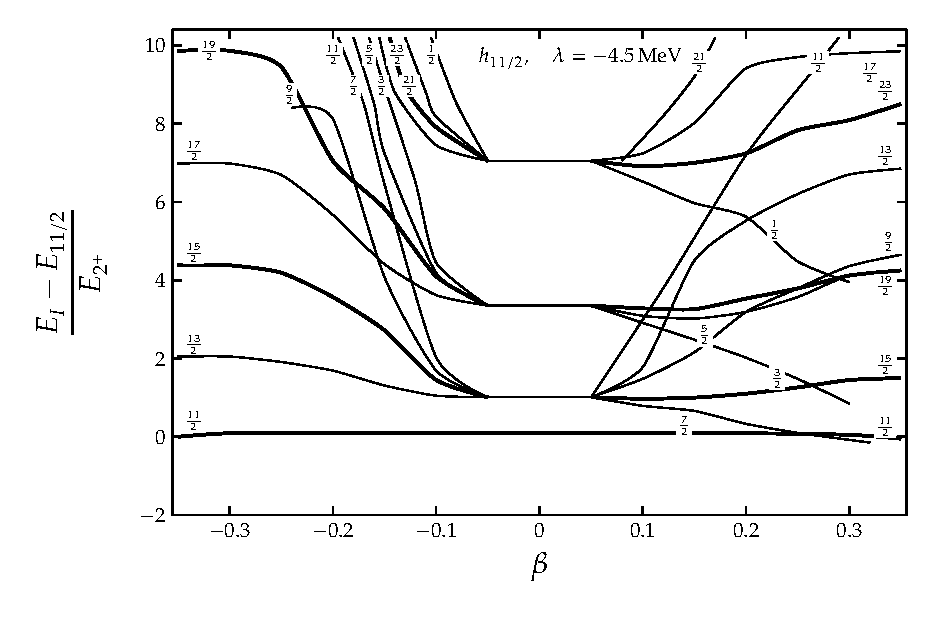
\includegraphics[width=0.75\textwidth]{pictures/3_10}
\par\end{centering}
\caption{\label{fig:3.10}轴对称粒子加转子模型中一个粒子处于 $1h_{11/2}$ 壳层的本征值随形变 $\beta$
的变化关系。图中绘制的是相对于 $I=11/2$ 能级的激发能。Fermi 面 $\lambda$ 位于整个 $1h_{11/2}$
轨道之下。（引自 \cite{St75a}。）}
\end{figure}

当然，能带的结构也依赖于 Fermi 面的位置。在此我们讨论的是壳层中仅有一个粒子的最简单情形。完全类似的情况是高 $j$ 壳层中仅有一个空穴。此时情况颠倒过来：在长椭球一侧是具有大
$\Omega$ 值的能级——即观测到强耦合方案；而在扁椭球一侧是具有小 $\Omega$ 值的能级，表现为解耦方案。

这些思考表明，基于此类高 $j$ 能级建立的转动带结构，为在过渡区通过实验区分长椭球形变与扁椭球形变提供了极其优秀的工具。

总结本小节的结果，我们可以得出：
\begin{enumerate}
\item[(i)] 在很多情况下，Coriolis 相互作用可以忽略。此时价核子绕核心的对称轴转动，并随核心改变其取向（强耦合，$\Delta I=1$）。
\item[(ii)] 在小形变且 Coriolis 相互作用强烈的情形下，价核子取向其角动量，或多或少独立于核心的取向。核心以 $\Delta I=2$
转动（弱耦合）。
\item[(iii)] 对于中等形变，由于相消效应的发生，转动顺排得以出现。价粒子使其角动量平行于集体角动量顺排（垂直于核心的对称轴），能谱再次呈现 $\Delta I=2$。
\end{enumerate}

\subsection{粒子加转子模型的若干应用}

将少数几个价粒子耦合到对称转子上的模型，已被用于极其广泛的情形来拟合实验转动带。总的来说它获得了极大的成功。在此我们不想详细讨论已被使用的众多不同版本，仅探讨几个具有代表性的典型例子。

\subsubsection{良好形变奇 A 核中的强混合带}

形变区奇 $A$ 核的能谱展现出许多清晰揭示强耦合图像的转动带。只有当粒子位于具有高 $j$ 值的单粒子壳层中（例如 Er 同位素区的
$1i_{13/2}$ 壳层）时，人们才会观测到严重畸变的能带\footnote{关于这些畸变带与邻近偶偶核回弯行为的比较，参见 \cite{SKS74}。}。在低
$I$ 值处，它们起初表现为 $\Delta I=1$ 的强耦合带，但很快就能观测到交错扭曲现象：满足 $I+1/2$ 为偶数的能级相对于
$I+1/2$ 为奇数的能级发生越来越大的位移，以致于最终分裂为两条各自具有 $\Delta I=2$ 的独立能带（参见\ref{fig:3.11}
中的正宇称带以及 \cite{BDL75}）。

\begin{figure}[H]
\begin{centering}
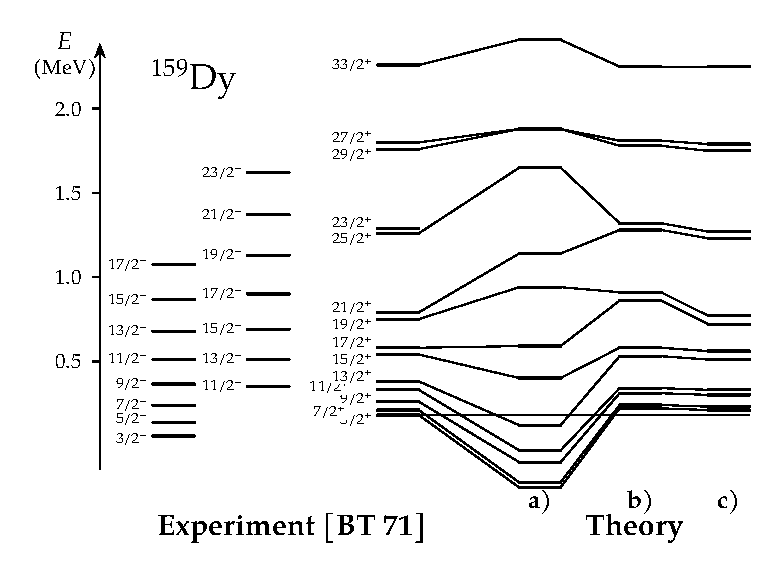
\includegraphics[width=0.75\textwidth]{pictures/3_11}
\par\end{centering}
\caption{\label{fig:3.11}$^{159}\text{Dy}$ 核中的三条转动带。$3/2^{-}$ 与 $11/2^{-}$
带是强耦合的（$\Delta I=1$）。带头为 $I=5/2$ 的正宇称带受到强烈微扰，如正文中所讨论。将其与三种理论计算进行了比较：(a)
无衰减 $\rho$ 的粒子加转子拟合；(b) 引入衰减因子 $\rho=0.5$ 的粒子加转子拟合；(c) 根据式 (3.56)
自洽确定的衰减。（引自 \cite{Ri77}。）}
\end{figure}

为了描述这些能带，人们通常在强耦合基 \ref{eq:3.25} 下对角化 Hamilton 量 \ref{eq:3.10}。单（准）粒子能量取自
Nilsson 模型，而形变 $\beta$（以及配对能隙 $\Delta$，参见第 6 章）等参数则用于拟合能谱。计算表明，只有引入一个削弱
Coriolis 相互作用的额外参数 $\rho$——即\emph{衰减因子}（attenuation factor），也就是用
$\rho\cdot H_{\text{cor}}$ 代替 $H_{\text{cor}}$ \cite{HRH70,LRB72,HK77}，才能够重现实验能谱。原始的
Coriolis 力被证实过于强烈，必须乘以因子 $\rho\sim0.4-0.8$ 予以缩减。通过这种唯象的衰减并合理选取模型的其他参数，我们能够成功重现这些畸变带，并发现对于低
$I$ 值（即较弱的 Coriolis 相互作用），体系处于 $\Delta I=1$ 的强耦合极限；然而对于更高的 $I$
值，Coriolis 力变得更强，并将具有高 $j$ 值的奇粒子平行于转动轴顺排。对于 $I\gtrsim j$ 的 $I$
值，体系具有转动顺排运动，即强烈的 $K$ 混合，能带分裂为 $(I-j)$ 为偶数时具有最大顺排 $\alpha=j$ 的优选态，以及
$(I-j)$ 为奇数时顺排较小的非优选态（$\alpha=j-1$）。对于由 $R=I-\alpha$ 给出的相同的核心角动量
$R$ 值，这两条带几乎是简并的（参见\ref{fig:3.11}）。

人们做出了若干尝试，在线性响应理论框架下将衰减因子解释为一种有效电荷 \cite{BPC72,HK75}。事实证明，这一问题与反冲项
\ref{eq:3.22} 的妥善处理紧密相关。认为反冲项已在拟合带头能量时被计入的观点并不成立，因为在单粒子情形下反冲项正比于
$\boldsymbol{j}^{2}-K^{2}$，具有强烈的 $K$ 依赖性并移动各带头的位置 \cite{ORG75}。

为了定性理解反冲项的作用，我们限制在仅有一个粒子的情形，并将粒子加转子 Hamilton 量 {[}\ref{eq:3.20} 等{]}
改写为如下形式 \cite{Kr79}：

\begin{equation}
H=H_{\text{intr}}+\frac{1}{2\mathcal{J}}\left(I(I+1)-\boldsymbol{j}^{2}\right)+H_{\text{cor}}'\label{eq:3.50}
\end{equation}
其中新的 Coriolis 项为

\begin{equation}
H_{\text{cor}}'=-\frac{1}{\mathcal{J}}(\boldsymbol{I}-\boldsymbol{j})\cdot\boldsymbol{j}_{\perp}=-\frac{1}{\mathcal{J}}\boldsymbol{R}\cdot\boldsymbol{j}=-\boldsymbol{\omega}\cdot\boldsymbol{j}\label{eq:3.51}
\end{equation}
其中集体角速度由下式给出：

\begin{equation}
\boldsymbol{\omega}=-\boldsymbol{R}/\mathcal{J}\label{eq:3.52}
\end{equation}
\ref{eq:3.51} 中的 Coriolis 项 $H_{\text{cor}}'$ 相比于 $H_{\text{cor}}$
{[}\ref{eq:3.23}{]} 发生了衰减。为了看清这一点，我们进入奇粒子几乎完全顺排于集体转动 $\boldsymbol{R}$
的极限情形。此时我们有

\begin{equation}
\boldsymbol{R}\simeq\boldsymbol{I}_{\perp}\left(1-\frac{\alpha}{I}\right)\label{eq:3.53}
\end{equation}
并发现 $H_{\text{cor}}'$ 在这种情形下正比于 $H_{\text{cor}}$：

\begin{equation}
H_{\text{cor}}'=\left(1-\frac{\alpha}{I}\right)H_{\text{cor}}=\rho\cdot H_{\text{cor}}\label{eq:3.54}
\end{equation}
带有一个依赖于 $I$ 的衰减因子：

\begin{equation}
\rho=1-\frac{\alpha}{I}\label{eq:3.55}
\end{equation}
只有在极高的 $I$ 值下衰减才会消失。

到目前为止，关于反冲项影响的讨论仅局限于该算符的纯单粒子部分。实际上，它还包含一个两体相互作用项 $\boldsymbol{j}_{ik}\cdot\boldsymbol{j}_{lm}a^{\dagger}_{i}a^{\dagger}_{l}a_{m}a_{k}$，它产生了与核心粒子的相互作用。我们可以在平均场近似下处理该项
\cite{Ri77}，最终得到一个自洽衰减因子：

\begin{equation}
\rho=1-\frac{\langle j_{1}\rangle}{\sqrt{I(I+1)-\langle j^{2}_{3}\rangle}}\label{eq:3.56}
\end{equation}
在完全顺排的极限下，它过渡到\ref{eq:3.55} 的形式。我们还可以证明，这种近似等价于 cranking 模型（参见 3.4
节）。在自洽 cranking 模型框架下对奇 $A$ 核转动带的微观处理中（参见 7.7 节），Coriolis 相互作用的衰减被自动包含进来了
\cite{RMB74,RM74}。

\subsubsection{偶偶核中的回弯现象}

回弯现象（参见 3.2.4 节）已被 Stephens 和 Simon \cite{SS72a} 解释为 $1i_{13/2}$
壳层中两个中子的顺排。如果这两个中子不是绕 3 轴旋转，而是沿原子核的转动轴顺排，这便增加了额外的 $13/2+11/2=12$
个单位的角动量。因此，原子核可以通过添加单粒子角动量来降低其集体转动，同时增加其总角动量。

为了在数学上描述这一物理构想，Stephens 和 Simon 对角化了 Hamilton 量 \ref{eq:3.10}（包含
Coriolis 项的衰减），所选取的基底为未受微扰核心的 Slater 行列式

\[
|\Phi_{0}\rangle=|IMK=0\rangle
\]
以及两准粒子激发态（参见第 7 章）：

\begin{equation}
|\Phi_{K}\rangle=\beta^{\dagger}_{K_{1}}\beta^{\dagger}_{K_{2}}|IMK=K_{1}+K_{2}\rangle\label{eq:3.57}
\end{equation}
其中 $\beta^{\dagger}_{K}$ 是 $1i_{13/2}$ 壳层中处于 $\Omega=K$ 态的准粒子产生算符。

对于低 $I$ 值，晕态主要由纯转子的零准粒子态 $|\Phi_{0}\rangle$ 给出。激发带是两准粒子带。对于更高的 $I$
值，粒子将其角动量沿转动轴顺排，其中一个顺排至 $\alpha=j=13/2$，第二个顺排至 $\alpha=j-1=11/2$。这样我们发现态
$\Phi_{0}$ 与 $\Phi_{K}$（$K=0,1,\dots$）发生混合，并在完全顺排的极限下达到如下形式的两准粒子态{[}参见\ref{eq:3.44}{]}：

\begin{equation}
|\Phi\rangle_{\text{al}}=\sum_{K_{1}K_{2}}d^{j}_{K_{1}j}\left(-\frac{\pi}{2}\right)d^{j}_{K_{2}j-1}\left(-\frac{\pi}{2}\right)\beta^{\dagger}_{K_{1}}\beta^{\dagger}_{K_{2}}|IMK_{1}+K_{2}\rangle\label{eq:3.58}
\end{equation}
它可以示意性地写作 $\tilde{\beta}^{\dagger}_{j}\tilde{\beta}^{\dagger}_{j-1}|\Phi_{0}\rangle$，其中
$\tilde{\beta}^{\dagger}_{\alpha}$ 是沿 1 轴量子化的准粒子算符。

Stephens 和 Simon \cite{SS72a} 利用这一方法相当好地重现了实验上的回弯能谱。然而，由于他们未曾计入由
Coriolis 反配对效应引起的对关联的渐进变化，他们无法获得低自旋值下对 $I(I+1)$ 定律的偏离。

尽管该模型适当地描述了两个顺排粒子的重要效应，但它无法使我们断定是否存在任何其他机制可能成为观测到的回弯现象的起源。为了判决它究竟是由形状变化、向正常流体态的相变还是顺排过程所引起的，人们必须开展计入所有这些自由度的微观计算。此类研究已经展开（参见
7.7 节）。它们表明两个粒子的转动顺排是最主要的效应。在所有含有高 $j$ 壳层的核中都可以发现这一过程。至于它们是否产生回弯，最终取决于相互作用矩阵元的强度（能级交叉处两能带之间的相互作用）：只有在弱矩阵元的情形下，我们才会观测到突变跃迁，即回弯现象\footnote{Bengtsson 等人 \cite{BHM78} 发现该相互作用作为化学势 $\lambda$ 的函数呈现振荡行为。对该事实的解释参见
\cite{FPS80} 及其所列参考文献。}。

\subsection{三轴粒子加转子模型}

我们在 1.5.3 节中已经看到，Davydov 等人 \cite{DF58} 利用三轴转子来解释某些过渡核中低激发的 $2^{+}$
态。通过将一个外层粒子耦合到三轴转子上，该模型也可以推广到奇 $A$ 核 \cite{Pa61,HS62,PR62,PS65,MSD74,Me75,FT75,TF75,Le76,DF77,LLR78}。它已被应用于外层粒子处于高
$j$ 壳层的情形，并在描述许多过渡核的能级与衰变纲图方面显示出极强的威力\footnote{关于三轴转子模型向多粒子组态的推广，参见 \cite{TNV77,YTF77,TYF77,YTF78}。}。然而目前尚缺乏微观基础。利用微观理论计算这些质量区域的静态能量势能面，并未展现出三轴形变处存在深极小值来为此简易物理图像提供依据。事实上，还存在基于振动图像的其他模型
\cite{AP76,PVD77,YNN76}，它们同样能够重现这些能谱。目前尚不清楚过渡核的这两种物理图像之间是否存在内在联系。

在接下来的讨论中，我们限制在一个高 $j$ 壳层（例如 $1h_{11/2}$）中的单个外层粒子耦合到三轴转子的情形。在此情形下，Hamilton
量具有如下形式 \cite{MSD74}：

\begin{equation}
h=\sum^{3}_{i=1}\frac{R^{2}_{i}}{2\mathcal{J}_{i}}+h_{0}+kr^{2}\beta\left\{ \cos\gamma\,Y_{20}+\sin\gamma\,\frac{1}{\sqrt{2}}\left(Y_{22}+Y_{2-2}\right)\right\} \label{eq:3.59}
\end{equation}
转动惯量 $\mathcal{J}_{i}$ 对 $\beta,\gamma$ 的依赖关系取自无旋流模型{[}式 (1.48){]}，仅对其整体常数进行调节。常数
$k$ 由 Nilsson 方案中 $j$ 壳层的分裂给出。$h_{0}$ 是球形谐振子 Hamilton 量。通常也计入具有常能隙
$\Delta$ 的单粒子配对场。

\ref{fig:3.12} 给出了在典型形变 $\beta=54A^{-2/3}$ 下，Hamilton 量 \ref{eq:3.59}
的能谱作为 $\gamma$ 的函数。在长椭球一侧（$\gamma=0^{\circ}$）和扁椭球一侧（$\gamma=60^{\circ}$），我们再次看到与\ref{fig:3.10}
中相同的能谱。然而，这两个极限现在是通过 $(\beta,\gamma)$ 平面内一条保持形变 $\beta$ 恒定的圆弧（图
1.4）相连接的。我们不再穿过 $\beta=0$ 处的弱耦合极限。在这两端，能谱对三轴参数 $\gamma$ 的依赖性并不十分剧烈。从强耦合方案到解耦方案的实质性转变发生在
$\gamma=30^{\circ}$ 附近的相对狭窄的 $\gamma$ 区域内。在弱形变过渡核中有许多能谱能够通过 $20^{\circ}$
到 $40^{\circ}$ 之间的 $\gamma$ 值极好地重现。通过在可变转动惯量（VMI）模型类型的计算中计入转动惯量的变化，这种一致性还可以得到进一步改善
\cite{FT75}。

\begin{figure}[H]
\begin{centering}
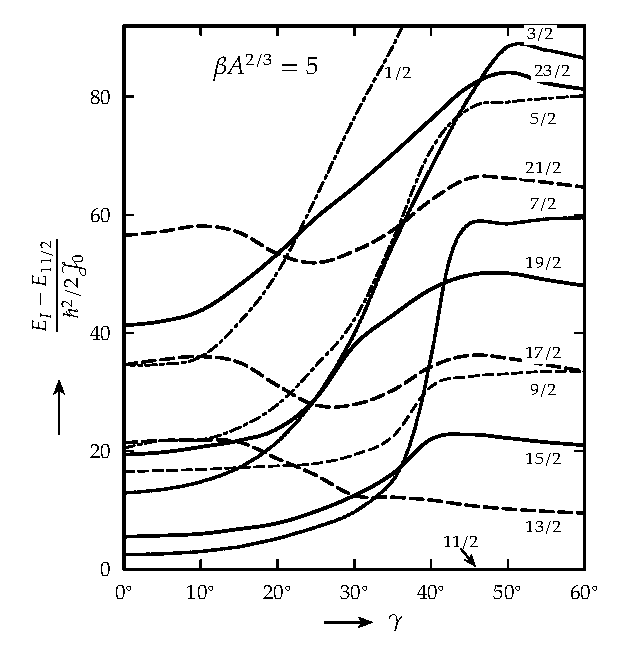
\includegraphics[width=0.75\textwidth]{pictures/3_12}
\par\end{centering}
\caption{\label{fig:3.12}一个 $j=11/2$ 粒子与非对称转子耦合的能谱，展示所有 $I\leqslant23/2$
的晕能级作为 $\gamma$ 的函数。（引自 \cite{MSD74}。）}
\end{figure}

一个奇高 $j$ 粒子与旋转三轴核心耦合系统的动力学行为由三种物理效应决定（参见 \cite{Me75}）：
\begin{enumerate}
\item[(i)] 核心倾向于绕具有最大转动惯量的轴旋转，以极小化转动能。
\item[(ii)] 在形变势阱中运动的粒子倾向于与核心取得最大的质量重叠，因为在此情形下其势能最小。
\item[(iii)] Coriolis 相互作用力图使粒子的角动量 $\boldsymbol{j}$ 与核心的角动量 $\boldsymbol{R}$
彼此顺排。
\end{enumerate}
对于高 $j$ 值，只要我们在 $j$ 壳层中仅有一个粒子，顺排效应便占据主导地位。由于顺排粒子的密度分布是以 $\boldsymbol{j}$
为对称轴的扁椭球，若核心为扁椭球（$\gamma=60^{\circ}$），对应于以 2 轴为对称轴，则条件 (ii) 得到最佳满足。然而在此情形下
$\mathcal{J}_{2}=0$，条件 (i) 受到了破坏。因此 $\boldsymbol{R}$ 将垂直于 2 轴，我们不再具有顺排。在三轴情形下，$\mathcal{J}_{2}$
不再为零，条件 (i)、(ii) 与 (iii) 可以全部同时得到满足。此时出现 $\boldsymbol{j}$ 与 $\boldsymbol{I}$
沿着 2 轴的顺排。事实上计算表明，奇粒子倾向于沿核心的 2 轴顺排。该轴起到近似对称轴的作用，其含义在于近似量子数 $K$ 与
$\Omega$（分别代表 $\boldsymbol{I}$ 与 $\boldsymbol{j}$ 在 2 轴上的投影）对于能级分类是有意义的。其结果是产生具有三轴转子特征的全新能级方案。

正如 Stephens 的转动顺排耦合方案那样，晕能级由 $\Omega=j$ 以及 $K=j,j+2,j+4$ 给出。对于这些能级，$\boldsymbol{I}$、$\boldsymbol{j}$、$\boldsymbol{R}$
以及 2 轴彼此平行。它们位于具有 $\Delta I=2$ 的通常抛物线上（参见\ref{fig:3.13}）。在轴对称情形下，顺排的方向在
1-2 平面内是任意的（通常选取 1 轴）；与之相反，非对称情形没有这种对称性，顺排明显青睐于 2 轴。这导致的推论是，在每一个晕能级上都存在自旋次序为
$\Delta I=1$ 的转动带。事实上，实验上已经观测到了这类能级 \cite{ABR75}。

\begin{figure}[H]
\begin{centering}
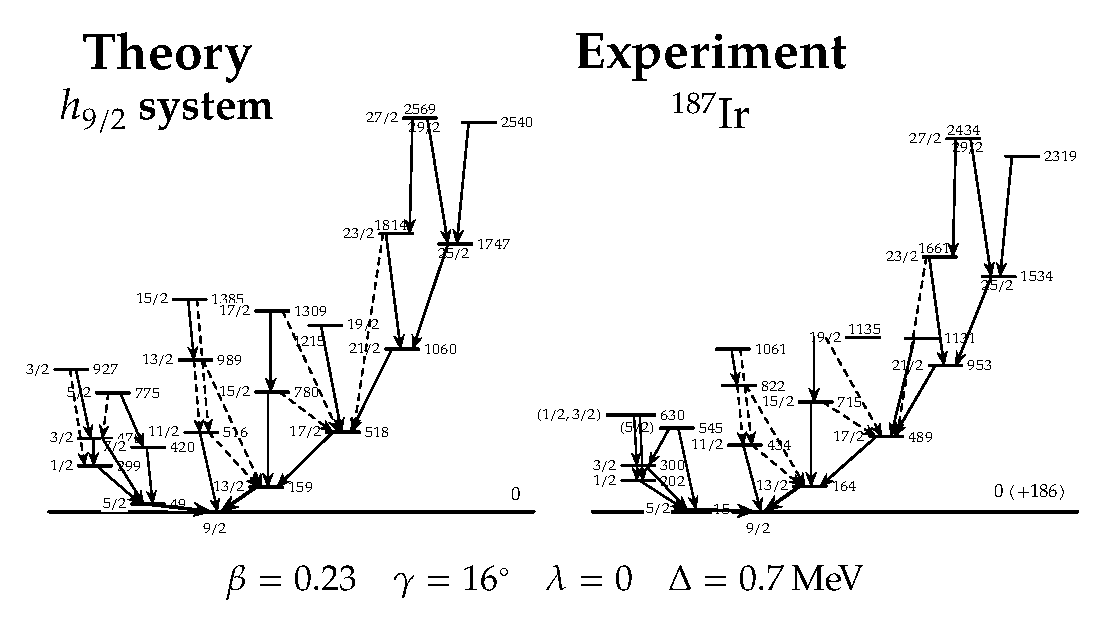
\includegraphics[width=0.75\textwidth]{pictures/3_13}
\par\end{centering}
\caption{\label{fig:3.13}$^{187}\text{Ir}$ 中负宇称态的 $1h_{9/2}$ 家族。（引自 \cite{Me75}。）}
\end{figure}


\subsection{电磁性质}

根据将系统划分为价粒子与核心的做法，电磁多极算符也相应地包含两部分贡献：

\begin{equation}
Q_{\lambda\mu}=Q^{(c)}_{\lambda\mu}+Q^{(p)}_{\lambda\mu}\label{eq:3.60}
\end{equation}
核心部分由式 (1.35) 给出，而 $Q^{(p)}$ 在式 (B.23)、(B.24) 中定义，其中对 $i$ 的求和仅限于价粒子的数目。

在接下来的讨论中，我们将限制在没有对关联的轴对称情形。随后将这些公式推广到更复杂的情形是相对简单的。

转子的磁偶极矩由式 (1.36) 给出为 $\boldsymbol{\mu}=g_{R}\mu_{N}\boldsymbol{R}$。因此对于
$M1$ 算符我们获得：

\begin{equation}
\boldsymbol{M}_{1}=\sqrt{\frac{3}{4\pi}}\mu_{N}g_{R}(\boldsymbol{I}-\boldsymbol{j})+\boldsymbol{M}^{(p)}_{1}\label{eq:3.61}
\end{equation}
磁偶极矩在式 (B.31) 中定义。利用\ref{eq:3.25} 的波函数并应用投影定理 (2.66)，对于 $K\neq1/2$
我们得到：

\begin{equation}
\mu=\sqrt{\frac{4\pi}{3}}\langle\Psi^{I}_{IK}|M_{1z}|\Psi^{I}_{IK}\rangle=\mu_{N}\left\{ g_{R}\frac{I(I+1)-K^{2}}{I+1}+g_{K}\frac{K^{2}}{I+1}\right\} \label{eq:3.62}
\end{equation}
其中我们以如下方式引入了回旋磁比 $g_{K}$：

\begin{align}
g_{K}\cdot K & =\frac{1}{\mu_{N}}\sqrt{\frac{4\pi}{3}}\langle\Phi_{K}|M^{(p)}_{13}|\Phi_{K}\rangle\nonumber \\
 & =\langle\Phi_{K}|g_{s}s_{3}+g_{l}l_{3}|\Phi_{K}\rangle\nonumber \\
 & =g_{l}K+(g_{s}-g_{l})\langle\Phi_{K}|s_{3}|\Phi_{K}\rangle\label{eq:3.63}
\end{align}
矩阵元 $\langle\Phi_{K}|s_{3}|\Phi_{K}\rangle$ 可以利用 Nilsson 波函数算出。对于
$K=1/2$，磁矩获得一个包含\ref{eq:3.30} 中解耦因子 $a$ 的额外贡献。

利用\ref{eq:3.62} 获得的磁矩已在广泛的原子核范围进行了计算 \cite[第 653 页]{MN59,NN65}，人们发现与实验数据的一致性通常质子优于中子。详细的研究表明，人们同样需要对
$g_{s}$ 引入极化电荷：$g^{\text{eff}}_{s}\simeq0.7g^{\text{free}}_{s}$（参见
\cite[第 302 页起]{BM75}）。

类似地，我们可以计算 $M1$ 跃迁的约化矩阵元。算符 $\boldsymbol{I}$ 不引起任何跃迁。对于其余部分我们利用式
(1.70)，对于 $K\neq1/2$ 且 $I_{i}\neq I_{f}$ 得到：

\begin{equation}
B(M1,I_{i}\to I_{f})=\frac{1}{2I_{i}+1}|\langle\Psi^{I_{f}}_{K}\|\boldsymbol{M}_{1}\|\Psi^{I_{i}}_{K}\rangle|^{2}=\frac{3}{4\pi}\mu^{2}_{N}(g_{K}-g_{R})^{2}K^{2}|C^{I_{i}\ 1\ I_{f}}_{K\ 0\ K}|^{2}\label{eq:3.64}
\end{equation}
这些 $M1$ 跃迁仅可能存在于奇 $A$ 核的转动带中。计算结果与实验符合得相当好 \cite{SBP67}。

再次利用式 (1.70)，我们还可以导出电四极跃迁的 $B(E2)$ 值。对于相同 $K$ 值的态之间的跃迁，由于核心具有巨大的
$Q_{0}$ 值，核心贡献远大于粒子贡献。因此粒子贡献可以忽略，我们得到：

\begin{equation}
B(E2,I_{i}\to I_{f})=Q^{2}_{0}\frac{5}{16\pi}|C^{I_{i}\ 2\ I_{f}}_{K\ 0\ K}|^{2}\label{eq:3.65}
\end{equation}
该方程用于确定出现在 $Q_{0}$ 中的形变实验值。在 2.8.6 节中我们看到它们与理论确定的形变相符合。因此，粒子加转子模型对于具有相同
$K$ 值的跃迁给出了适宜的 $E2$ 跃迁几率。

对于具有不同 $K$ 值的跃迁，集体部分消失。此类跃迁实际上非常微弱（$K$ 禁戒，$K$-forbidden），因为单粒子部分仅包含内禀系中
$r^{2}Y_{20}$ 的单粒子矩阵元。我们在 2.7.2 节中已经看到，它们与集体跃迁值相比是极其微小的。另一方面，纯单粒子模型无法解释球形核中的有效电荷（参见
2.7.2 节）。同样的困难在此再次出现。关于详细讨论，请参阅 Löbner 和 Malmskog 的论文 \cite{LM66}，其中包含了大量实验数据以及改进简易
Nilsson 估计的可能途径。

最后我们必须提及，上述考虑仅适用于纯 $K$ 带。对于 $K$ 混合带中的跃迁几率与电磁矩（例如转动顺排带或非对称转子中的能带），我们必须计入混合系数。

\section{Cranking 模型\protect\footnote{在本章中，我们仅讨论用于转动的 cranking 理论。然而，正如在 12.3.7 节中所讨论的，我们也可以将类似理论应用于一般的集体运动。}}

我们在上一节中已经看到，形变势阱中的粒子运动如何能够与刚性转子的概念联系起来。该模型在描述转动核乃至过渡核的能级结构方面取得了巨大的成功。然而，它并不存在直接了当的微观推导；特别是在该模型中人们无法微观计算惯性参数。

另一方面，几乎所有关于原子核转动的完全微观的理论，都以某种方式基于或关联于由 Inglis \cite{In54,In56} 以半经典方式引入的\emph{推引模型}（cranking
model）。正如我们在 11.4 节中将要看到的，至少在强形变且 $K$ 掺杂不太强烈（$K\ll I$）的极限下，它可以完全从量子力学推导出来。

Cranking 模型具有以下显著优点：
\begin{enumerate}
\item[(i)] 原则上，它提供了旋转原子核的完全微观描述。该模型没有引入冗余变量，因此我们能够在模型内部微观地计算转动惯性参数，并深入洞悉转动运动的动力学本质。
\item[(ii)] 它将集体角动量描述为各单粒子角动量之和。因此，集体转动、单粒子转动以及它们之间的所有过渡（例如解耦过程），都在相同的基准上得到了统一的处理。
\item[(iii)] 对于非常高的角动量，经典论据完全适用，该模型是完全正确的（即使在这一极限下量子力学推导不再有效 \cite{BMR70}）。
\end{enumerate}
该模型的局限性在于：
\begin{enumerate}
\item[(i)] 正如我们将看到的，它本质上是一个非线性理论。只有在小角动量极限下，人们才能利用微扰论将其线性化（得到转动惯量的 cranking
公式）。在一般情形下计算因此变得复杂，特别是在具有多个解的情况下。
\item[(ii)] 由此得到的波函数不是角动量算符的本征态。因此，先验地如何计算例如电磁跃迁几率并不清晰。事实上，我们在 11.4 节中将看到，cranking
模型的波函数在某种意义上仅是内部波函数，必须使用投影技术才能获得实验室坐标系中的波函数。
\end{enumerate}
在下文中，我们将给出通常的半经典推导（例如参见 \cite{Vi57b,So73}），并结合纯单粒子 Hamilton 量讨论 cranking
模型。随后几节中的许多论据，也可以直接推广到一般的两体 Hamilton 量中（参见 7.7 节）。

\subsection{Cranking 模型的半经典推导}

Cranking 模型的基本思想基于如下经典假设：如果引入一个以恒定角速度 $\boldsymbol{\omega}$ 绕空间固定轴转动的参考系，若角频率选取适当，核子在转动参考系中的运动将相当简单；特别是，核子可以被视为独立粒子，运动于一个随坐标系共同转动的平均势阱之中。

在 11.4 节中，我们将看到如何利用投影技术从量子力学推导出这一物理图像的结论。然而目前，出于其直观性，我们仍希望保留经典描述。同时，我们暂不考虑任何剩余相互作用。因此，我们假设一个具有固定形状、在空间中转动的单粒子势
$V$，相应地我们必须考虑含时的单粒子 Hamilton 量：

\begin{equation}
h(t)=\frac{\boldsymbol{p}^{2}}{2m}+V(\boldsymbol{r},t)\label{eq:3.66}
\end{equation}
以及对应的 Schrödinger 方程：

\begin{equation}
h(t)\psi(t)=\mathrm{i}\hbar\frac{\partial}{\partial t}\psi(t)\label{eq:3.67}
\end{equation}
引入相对于转动轴 $\boldsymbol{\omega}$ 的球坐标 $r,\theta,\varphi$，我们可以将 $V(t)$
的时间依赖性表示为如下形式。若 $V(\boldsymbol{r},0)$ 是 $t=0$ 时的势，则在时刻 $t$ 有：

\begin{equation}
V(\boldsymbol{r},t)=V(r,\theta,\varphi-\omega t,0)\label{eq:3.68}
\end{equation}
我们再次认识到，$V$ 仅当它依赖于 $\varphi$ 时才显含时间。换言之，$V$ 不应当绕转动轴具有轴对称性，因为对于量子力学系统，绕对称轴不可能存在集体转动（参见
1.5.1 节）。由于\ref{eq:3.68} 中 $V(t)$ 具有非常简明的时间依赖性，存在一个消除此时间依赖性的幺正变换：

\begin{equation}
U=\mathrm{e}^{\mathrm{i}\boldsymbol{\omega}\cdot\boldsymbol{l}t/\hbar}\label{eq:3.69}
\end{equation}
其中 $\boldsymbol{\omega}\cdot\boldsymbol{l}=(\hbar/\mathrm{i})\omega\,\partial/\partial\varphi$。$U$
产生了绕转动轴 $\boldsymbol{\omega}$ 转动角度 $\omega t$ 的操作。

我们发现含时算符满足

\begin{equation}
Uh(t)U^{-1}=h(0)\label{eq:3.70}
\end{equation}
并定义变换后的波函数：

\begin{equation}
\tilde{\psi}=U\psi\label{eq:3.71}
\end{equation}
满足

\begin{equation}
\mathrm{i}\hbar\dot{\tilde{\psi}}=\mathrm{i}\hbar U\dot{\psi}+\mathrm{i}\hbar\dot{U}\psi=(h(0)-\boldsymbol{\omega}\cdot\boldsymbol{l})\tilde{\psi}\label{eq:3.72}
\end{equation}
\ref{eq:3.72} 是一个含有显含时间无关的有效 Hamilton 量 $h_{\omega}$ 的含时 Schrödinger
方程。因此它可以按标准方法化为一个本征值问题求解：

\begin{equation}
h_{\omega}\tilde{\psi}=(h(0)-\boldsymbol{\omega}\cdot\boldsymbol{l})\tilde{\psi}=\epsilon_{\omega}'\tilde{\psi}\label{eq:3.73}
\end{equation}
其中 $\epsilon_{\omega}'$ 是有效 Hamilton 量的本征值（又称 Routhian 本征值）。为了获得原始
Hamilton 量的能量，我们必须计算：

\begin{equation}
E_{k}=\langle\psi|h(t)|\psi\rangle=\langle\tilde{\psi}|h(0)|\tilde{\psi}\rangle=\epsilon_{k}'+\boldsymbol{\omega}\cdot\langle\tilde{\psi}|\boldsymbol{l}|\tilde{\psi}\rangle\label{eq:3.74}
\end{equation}
项 $\boldsymbol{\omega}\cdot\boldsymbol{l}$ 通常被称为 Coriolis 项。

我们现在求解了转动势中的含时 Schrödinger 方程，并发现我们必须对角化一个显含时间无关的有效 Hamilton 量。我们想强调的是，我们并非先验地推导从转动坐标系所看到的
Hamilton 量，因为我们仅变换了坐标而未变换动量。事实上，在纯平动运动的情形下，我们会得到类似的结果{[}$h_{v}=h(0)-\boldsymbol{v}\cdot\boldsymbol{p}${]}，但由
Galilei 不变性我们要求从运动参考系看到的 Hamilton 量与静止参考系相同。尽管如此，事实表明在转动的特殊情况下，\ref{eq:3.73}
中的 $h_{\omega}$ 与转动系统中所看到的 Hamilton 量是完全恒等的 \cite[第 69 页]{Va56,Br64}。从项
$\boldsymbol{\omega}\cdot\boldsymbol{l}$ 中，我们可以同时导出 Coriolis 力与离心力。

对于具有自旋的系统，产生转动的算符为 $\boldsymbol{j}=\boldsymbol{l}+\boldsymbol{s}$。转动轴的取向通常选取为平行于
$x$ 轴，因为人们理解转动轴垂直于对称轴（在 $\omega=0$ 时对称轴为 $z$ 轴）。对于更高的角动量，人们也研究非对称单粒子势。尽管如此，我们仍要求
$\boldsymbol{\omega}$ 平行于势的一个主轴。因此，cranking 模型的多体 Hamilton 量由下式给出（其中
$J_{x}=\sum^{A}_{i=1}j^{(i)}_{x}$）：

\begin{equation}
H_{\omega}=H-\omega J_{x}=\sum^{A}_{i=1}h^{(i)}_{\omega}\label{eq:3.75}
\end{equation}
其中 $H$ 是形变单粒子 Hamilton 量之和。

在 cranking 模型中，我们现在必须对角化 $H_{\omega}$，所得的基态波函数 $\Phi_{\omega}$ 是一个
Slater 行列式。正如在普通壳模型（$\omega=0$）中一样，出现了一个问题：应当如何填充分配单粒子势中的能级，以获得任意给定角动量下的最低能量状态（晕能级）？这一问题的答案（在
11.4 节中给出）是，我们必须极小化能量 $E'=\langle\Phi|H-\omega J_{x}|\Phi\rangle$，也就是说，我们必须在转动参考系中按通常的方式从低到高填充有效能级。

对于实验室坐标系中的能量，由\ref{eq:3.74} 我们得到：

\begin{equation}
E(\omega)=\langle\Phi_{\omega}|H|\Phi_{\omega}\rangle=\langle\Phi_{\omega}|H_{\omega}|\Phi_{\omega}\rangle+\omega\langle\Phi_{\omega}|J_{x}|\Phi_{\omega}\rangle\label{eq:3.76}
\end{equation}
由于 $E(\omega)$ 不能依赖于 $\omega$ 的符号，人们发现：

\begin{equation}
E(\omega)=E(0)+\frac{1}{2}\mathcal{J}_{1}\omega^{2}+\dots\label{eq:3.77}
\end{equation}
并且，由于在 $\omega=0$ 时 $\langle\Phi_{0}|J_{x}|\Phi_{0}\rangle=0$，

\begin{equation}
J(\omega)=\langle\Phi_{\omega}|J_{x}|\Phi_{\omega}\rangle=\mathcal{J}_{2}\omega+\dots\label{eq:3.78}
\end{equation}
利用 $E'(\omega)$ 是 $H_{\omega}$ 的最低本征值这一事实，我们可以证明常数 $\mathcal{J}_{1}$
与 $\mathcal{J}_{2}$ 是相等的 \cite{Sch61}：

\begin{equation}
\mathcal{J}_{1}=\mathcal{J}_{2}\label{eq:3.79}
\end{equation}
根据 Ritz 变分原理，我们获得 $\Phi_{\omega}$ 作为如下方程的解：

\begin{equation}
\delta\langle\Phi|H-\omega J_{x}|\Phi\rangle=0\label{eq:3.80}
\end{equation}
其中 $|\Phi\rangle$ 是所有可能 Slater 行列式集合中的任意一员。如果我们将 $|\Phi\rangle$
限制在子集 $\{\Phi_{\omega'}\}$ 中（其中 $\Phi_{\omega'}$ 是 $H-\omega'J_{x}$
的本征函数，$\omega'$ 遍历所有实数），该条件同样满足。于是由\ref{eq:3.80} 得到：

\begin{equation}
\left.\frac{\mathrm{d}}{\mathrm{d}\omega'}\langle\Phi_{\omega'}|H|\Phi_{\omega'}\rangle\right|_{\omega'=\omega}-\omega\left.\frac{\mathrm{d}}{\mathrm{d}\omega'}\langle\Phi_{\omega'}|J_{x}|\Phi_{\omega'}\rangle\right|_{\omega'=\omega}=0\label{eq:3.81}
\end{equation}
或者

\[
\mathcal{J}_{1}=\left.\frac{1}{\omega}\frac{\mathrm{d}}{\mathrm{d}\omega}E(\omega)\right|_{\omega=0}=\left.\frac{\mathrm{d}}{\mathrm{d}\omega}J(\omega)\right|_{\omega=0}=\mathcal{J}_{2}
\]
由\ref{eq:3.80} 我们还可以导出正则关系：

\begin{equation}
\omega=\frac{\mathrm{d}E}{\mathrm{d}J}\label{eq:3.82}
\end{equation}
为了与实验进行比较，我们必须确定角速度的值。Inglis \cite{In54} 建议至少在半经典意义上通过要求

\begin{equation}
J=\langle\Phi_{\omega}|J_{x}|\Phi_{\omega}\rangle=\sqrt{I(I+1)}\label{eq:3.83}
\end{equation}
来包含零点量子涨落。在一阶近似下我们得到

\begin{equation}
\omega=\frac{\sqrt{I(I+1)}}{\mathcal{J}_{1}}\label{eq:3.84}
\end{equation}
并由\ref{eq:3.77} 得到：

\begin{equation}
E(I)=E(0)+\frac{1}{2\mathcal{J}_{1}}I(I+1)\label{eq:3.85}
\end{equation}
对于更高的 $\omega$ 值，将出现对该 $I(I+1)$ 定律的偏离。一般而言，转动惯量定义为

\begin{equation}
\mathcal{J}=\frac{J}{\omega}\label{eq:3.86}
\end{equation}
到目前为止，我们仅研究了完全独立的粒子运动，这里的含义是我们甚至忽略了转动对平均场本身的反作用影响。在 7.7 节中我们将展示如何将该效应自洽地予以考虑。

\subsection{Cranking 公式}

在纯 $I(I+1)$ 能谱的情形下，我们只需计算一个常数，即转动惯量。它已经被 $2^{+}$ 态所完全确定，因此对于如此小的
$I$ 值应用微扰论显得十分有意义。

我们从形变势阱中被填充至 Fermi 面的未微扰系统出发。Fermi 面以下的能级被称为空穴态（指标 $i,l,\dots$）；Fermi
面以上的能级被称为粒子态（指标 $m,m',\dots$）。壳模型基底由基态 $|\Phi_{0}\rangle$、粒子-空穴态（ph
态）$|mi\rangle=a^{\dagger}_{m}a_{i}|\Phi_{0}\rangle$、2p-2h 态等构成。微扰
$\omega J_{x}$ 是一个单体算符，因此一次只能激发一个 ph 对。因此，对于一阶微扰波函数我们得到：

\begin{equation}
|\Phi\rangle=|\Phi_{0}\rangle+\omega\sum_{mi}\frac{\langle mi|J_{x}|\Phi_{0}\rangle}{\epsilon_{m}-\epsilon_{i}}a^{\dagger}_{m}a_{i}|\Phi_{0}\rangle\label{eq:3.87}
\end{equation}
其中 $\epsilon_{i}$ 与 $\epsilon_{m}$ 是 Hamilton 量 $H$ 的单粒子能量。至 $\omega$
的一阶，$J_{x}$ 的期望值为

\begin{equation}
J=\langle\Phi|J_{x}|\Phi\rangle=2\omega\sum_{mi}\frac{|\langle mi|J_{x}|\Phi_{0}\rangle|^{2}}{\epsilon_{m}-\epsilon_{i}}\label{eq:3.88}
\end{equation}
结合\ref{eq:3.78}，这给出了转动惯量\footnote{在分子物理学中，Wick \cite{Wi48} 曾推导出类似的公式。}：

\begin{equation}
\mathcal{J}_{\text{Inglis}}=2\sum_{mi}\frac{|\langle mi|J_{x}|\Phi_{0}\rangle|^{2}}{\epsilon_{m}-\epsilon_{i}}\label{eq:3.89}
\end{equation}
这就是著名的 Inglis 转动惯量公式 \cite{In54,BM55}。

由该公式算出的转动惯量通常非常接近刚体转动惯量的值{[}式 (1.49){]}。事实上，我们在 3.4.3 节中将看到，在纯各向异性谐振子势的情形下这甚至是一个严格的结果。Lüders
\cite{Lu60} 证明，对于任何独立粒子模型在大粒子数极限下均成立此结论（亦参见 \cite{AB59,Ro59,SB64,Da75,KG78}）。

我们可以定性地理解这一结果：只要我们认识到形变静态势中基态的速度分布几乎是各向同性的（参见 13.3 节），并且在转动系统中这一事实并未因
Coriolis 力或离心力而改变（参见 \cite{BJ76b}）。此时在内禀系中没有净流动，而在实验室参考系中我们观测到刚体转动的速度分布。

正如我们在 1.5.1 节中所见，实验上的转动惯量比它们的刚体值小 2 到 3 倍。Bohr 和 Mottelson \cite{BM55,Mo56}
早就指出，剩余两体相互作用会大幅降低这些数值。在这方面最重要的影响是对关联型的相互作用。由于在单粒子描述中它们可以在 BCS 形式体系内非常方便地予以包含（参见第
6 章），我们在此给出所谓的 Belyaev 公式 \cite{Be59,Be61} 的推导，它是包含了对关联的 Inglis \ref{eq:3.89}
的推广。（不熟悉该体系的读者请参阅第 6 章。）

在这种情形下，$|\text{BCS}\rangle$ 代表 BCS 基态 (6.31)，激发态由两准粒子态 $\alpha^{\dagger}_{k}\alpha^{\dagger}_{k'}|\text{BCS}\rangle$、四准粒子态等给出。与\ref{eq:3.87}
完全类似地，我们得到受微扰的波函数：

\begin{equation}
|\Phi\rangle=|\text{BCS}\rangle+\omega\sum_{k<k'}\frac{\langle\text{BCS}|J_{x}|kk'\rangle}{E_{k}+E_{k'}}\alpha^{\dagger}_{k}\alpha^{\dagger}_{k'}|\text{BCS}\rangle\label{eq:3.90}
\end{equation}
其中 $E_{k}+E_{k'}$ 是准粒子对 $k,k'$ 的激发能量。准粒子能量由下式给出：

\begin{equation}
E_{k}=\sqrt{(\epsilon_{k}-\lambda)^{2}+\Delta^{2}}\label{eq:3.91}
\end{equation}
仿照\ref{eq:3.88} 与 \ref{eq:3.89}，我们求得转动惯量：

\begin{equation}
\mathcal{J}_{\text{Belyaev}}=2\sum_{k<k'}\frac{|\langle\text{BCS}|J_{x}|kk'\rangle|^{2}}{E_{k}+E_{k'}}\label{eq:3.92}
\end{equation}
由式 (E.16)，我们求得 $J_{x}$ 的两准粒子矩阵元，并最终得到：

\begin{equation}
\mathcal{J}_{\text{Belyaev}}=2\sum_{k,k'>0}\frac{|\langle k|j_{x}|k'\rangle|^{2}}{E_{k}+E_{k'}}\left(u_{k}v_{k'}-u_{k'}v_{k}\right)^{2}\label{eq:3.93}
\end{equation}
与\ref{eq:3.89} 相比，该转动惯量公式确实给出了大幅降低的值。导致这一降低的有两个效应：
\begin{enumerate}
\item[(i)] 能量分母远大于\ref{eq:3.89} 中的粒子-空穴能量。参数 $\Delta$ {[}\ref{eq:3.91}{]}
对 Fermi 面附近的关键能级产生了至少 $2\Delta\sim2\,\text{MeV}$ 的能隙；
\item[(ii)] 因子 $(u_{k}v_{k'}-u_{k'}v_{k})^{2}$ 通常明显小于 1。
\end{enumerate}
BCS 理论中转动惯量相比于刚体值的降低，对应于原子核转动时部分核子的“超流滑移”（superfluid slippage）\cite{Mi59,Mi60}。

针对真实原子核的大规模数值计算 \cite{GR60b,NP61,MT75} 显示出与实验值极其显著的符合。正如我们在下一小节中将看到的，将
Inglis 或 Belyaev 公式应用于自洽波函数（即在对应于能量极小值的形变下计算出的波函数）是至关重要的。在大多数此类计算中，这是通过在实验观测到的形变下使用
Nilsson 波函数与能量、并采用实验确定的配对能隙 $\Delta$ 来实现的（亦参见 \cite{MN59}）。

这些计算给出的转动惯量大致落在（过小的）无旋流值与（过大的）刚体值之间，其巨大的成功给予我们极大的信心：将转动核视为形变超流多体系统的物理图像是完全正确的。

当然，我们还可以研究剩余相互作用对转动惯量的进一步影响。这可以在线性响应理论框架下进行（参见 8.5.3 节与 \cite{MSV72}）。在此类理论中，由
Coriolis 算符 $J_{x}$ 代表的外场可以激发核心的虚振动，这些振动反过来对转动惯量产生影响。存在两类此类振动：表面振荡（ph
振动，对应于拉伸效应），以及对关联中的振荡（pp 振动，参见 8.3.5 节）。此类计算的综合结果是，这两种效应大致相互抵消，我们得到的转动惯量数值（\ref{fig:3.14}）与
BCS 理论给出的结果基本相同。

\begin{figure}[H]
\begin{centering}
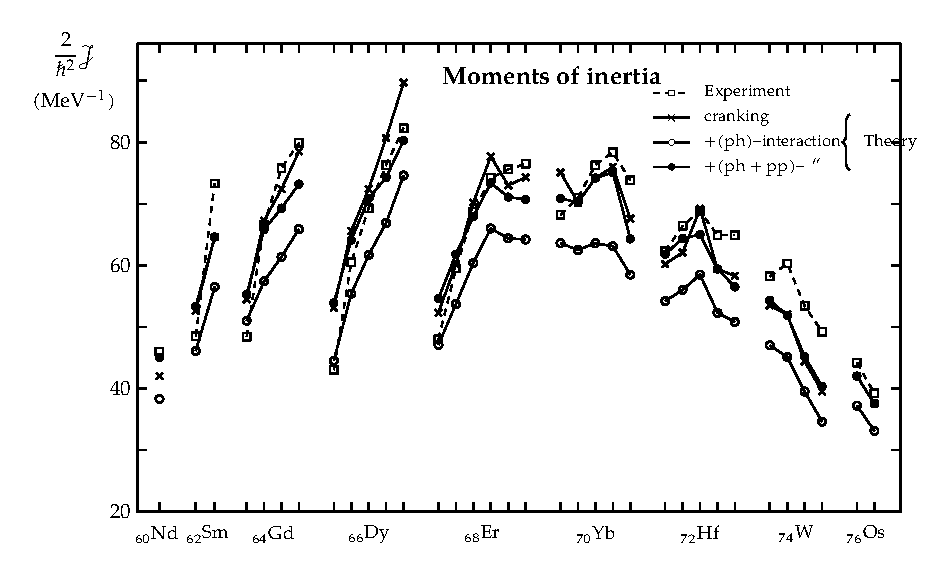
\includegraphics[width=0.75\textwidth]{pictures/3_14}
\par\end{centering}
\caption{\label{fig:3.14}稀土核中的转动惯量。方块表示实验值 \cite{NP61}；十字是由 Belyaev 公式 (3.93)
算得的结果。空心圆圈仅计入了拉伸效应（ph 相互作用）；除此之外，实心圆圈还计入了反配对效应（pp 相互作用）。（引自 \cite{MSV72}。）}
\end{figure}

我们现在已经讨论了应用微扰论计算 $J_{x}$ 的期望值（即转动惯量）。以类似的方式，我们还可以计算旋转核的其他性质，例如回旋磁比
$g_{R}$ 或第一 $2^{+}$ 态的磁矩。由于磁矩 $\mu$ 定义为 $M_{1z}$ 在态 $|I,M=I\rangle$
中的期望值{[}式 (B.31){]}，而 cranking 模型的波函数不是角动量的本征态，此时如何计算 $\mu$ 尚不明确。在
11.4 节中我们将看到必须应用投影技术。在最低阶近似下，我们获得一个非常简单的结果，它在 cranking 模型的半经典图像中极易理解：

\begin{equation}
\mu=\langle\Phi_{\omega}|M_{x}|\Phi_{\omega}\rangle\label{eq:3.94}
\end{equation}
因此我们可以通过下式定义回旋磁比 (1.37)：

\begin{equation}
\mu=g_{R}J=g_{R}\langle\Phi_{\omega}|J_{x}|\Phi_{\omega}\rangle\label{eq:3.95}
\end{equation}
由\ref{eq:3.90}，在一阶微扰论下我们得到：

\begin{equation}
g_{R}=\frac{1}{\mathcal{J}}\sum_{k,k'>0}\frac{\langle k|j_{x}|k'\rangle\langle k'|M_{x}|k\rangle+\text{c.c.}}{E_{k}+E_{k'}}\left(u_{k}v_{k'}-u_{k'}v_{k}\right)^{2}\label{eq:3.96}
\end{equation}
利用这些公式计算出的数值小于液滴模型的值 $g_{R}=Z/A$ {[}式 (1.37){]}，并与实验数据符合得相当好 \cite{MSV72}。

正如我们在 3.2 节中所见，当我们走向更高的角动量时，将出现对 $I(I+1)$ 定律的偏离。为了计算与这些偏离相联系的 $B$
与 $C$ 系数{[}式 (3.1){]}，人们使用了更高阶的微扰论，并计入了剩余相互作用的效应 \cite{Ma65,Ma67a,MR70}，其中最重要的效应是所谓的
Coriolis 反配对（CAP）效应，我们将在 7.7 节中对此进行讨论。正如我们将看到的，只有在自旋极高（$I>30$ 或 40）的态上，人们才能预期对关联彻底消失。

\subsection{转动各向异性谐振子}

我们在 2.8.3 节中已经看到，各向异性谐振子可以解析求解，并且它至少为形变核提供了一个定性模型。事实表明，它在转动参考系中同样可以解析求解（参见
\cite{Va56,Ze75,RBK75,GMZ78}），因为 $l_{x}=yp_{z}-zp_{y}$ 在坐标 $x,y,z$
和动量 $p_{x},p_{y},p_{z}$ 中是一个二次型。

我们可以暂且忽略自旋，因为势阱不依赖于自旋（Coriolis 算符中的项 $-\omega s_{x}$ 可以在自旋空间中独立对角化，仅产生一个对角贡献）。此时
Hamilton 量具有形式：

\begin{equation}
h_{\omega}=-\frac{\hbar^{2}}{2m}\nabla^{2}+\frac{1}{2}m\left(\omega^{2}_{x}x^{2}+\omega^{2}_{y}y^{2}+\omega^{2}_{z}z^{2}\right)-\omega\left(yp_{z}-zp_{y}\right)\label{eq:3.97}
\end{equation}
我们引入 $x,y,z$ 方向谐振子玻色子的产生和湮灭算符 $a_{x},a_{y},a_{z}$：

\begin{align}
x & =\left(\frac{\hbar}{2m\omega_{x}}\right)^{1/2}\left(a_{x}+a^{\dagger}_{x}\right),\quad p_{x}=\frac{\hbar}{\mathrm{i}}\left(\frac{m\omega_{x}}{2\hbar}\right)^{1/2}\left(a_{x}-a^{\dagger}_{x}\right)\nonumber \\
y & =\left(\frac{\hbar}{2m\omega_{y}}\right)^{1/2}\left(a_{y}+a^{\dagger}_{y}\right),\quad p_{y}=\frac{\hbar}{\mathrm{i}}\left(\frac{m\omega_{y}}{2\hbar}\right)^{1/2}\left(a_{y}-a^{\dagger}_{y}\right)\label{eq:3.98}\\
z & =\left(\frac{\hbar}{2m\omega_{z}}\right)^{1/2}\left(a_{z}+a^{\dagger}_{z}\right),\quad p_{z}=\frac{\hbar}{\mathrm{i}}\left(\frac{m\omega_{z}}{2\hbar}\right)^{1/2}\left(a_{z}-a^{\dagger}_{z}\right)\nonumber 
\end{align}
利用这些算符，$h_{\omega}$ 具有形式：

\begin{align}
h_{\omega} & =\hbar\omega_{x}\left(a^{\dagger}_{x}a_{x}+\frac{1}{2}\right)+\hbar\omega_{y}\left(a^{\dagger}_{y}a_{y}+\frac{1}{2}\right)+\hbar\omega_{z}\left(a^{\dagger}_{z}a_{z}+\frac{1}{2}\right)\nonumber \\
 & \quad+\frac{\hbar\omega}{2\sqrt{\omega_{y}\omega_{z}}}\left\{ (\omega_{y}-\omega_{z})\left(a^{\dagger}_{y}a^{\dagger}_{z}+a_{y}a_{z}\right)+(\omega_{y}+\omega_{z})\left(a^{\dagger}_{y}a_{z}+a^{\dagger}_{z}a_{y}\right)\right\} \label{eq:3.99}
\end{align}
\ref{eq:3.99} 中的 Coriolis 算符包含两部分贡献。第一部分产生或湮灭两个振子量子；因此它将主量子数为 $N$
与 $N\mp2$ 的壳层耦合起来\footnote{在微小形变极限下（$\omega_{y}\to\omega_{z}$）该项消失，因此常常被忽略 \cite{ALL76}。}。第二部分保持量子总数守恒，但将振子量子从
$y$ 方向转移到 $z$ 方向，反之亦然。

\subsubsection{Inglis 公式}

首先我们想在微扰论中处理 Coriolis 项。在 Inglis \ref{eq:3.89} 中，$\Delta N=\pm2$
部分具有能量分母 $\pm\hbar(\omega_{y}+\omega_{z})$，而 $\Delta N=0$ 部分具有分母
$\pm\hbar(\omega_{y}-\omega_{z})$。算符 $a,a^{\dagger}$ 的矩阵元由式 (C.12f)
给出：

\[
\langle n-1|a|n\rangle=\sqrt{n},\quad\langle n+1|a^{\dagger}|n\rangle=\sqrt{n+1}
\]
由\ref{eq:3.89} 我们得到：

\begin{equation}
\mathcal{J}_{\text{Inglis}}=\frac{\hbar}{2\omega_{y}\omega_{z}}\left\{ \frac{(\omega_{y}-\omega_{z})^{2}}{\omega_{y}+\omega_{z}}(N_{y}+N_{z})+\frac{(\omega_{y}+\omega_{z})^{2}}{\omega_{y}-\omega_{z}}(N_{z}-N_{y})\right\} \label{eq:3.100}
\end{equation}
其中

\begin{equation}
N_{x,y,z}=\sum^{A}_{i=1}\left(n_{x,y,z}+\frac{1}{2}\right)_{i}\label{eq:3.101}
\end{equation}
满足关系：

\begin{equation}
\bar{x}^{2}=\frac{1}{A}\sum^{A}_{i=1}\langle x^{2}\rangle_{i}=\frac{1}{A}\frac{\hbar}{m\omega_{x}}\sum^{A}_{i=1}\left(n_{x}+\frac{1}{2}\right)_{i}=\frac{\hbar}{Am\omega_{x}}N_{x}\label{eq:3.102}
\end{equation}
对于接下来的讨论极为重要的是\emph{自洽性条件} \cite{BM75}：即由 $\omega_{x},\omega_{y},\omega_{z}$
决定的势阱形状必须与由 $\bar{x}^{2},\bar{y}^{2},\bar{z}^{2}$ 给出的密度分布具有相同的形状：

\begin{equation}
\bar{x}^{2}:\bar{y}^{2}:\bar{z}^{2}=\frac{1}{\omega^{2}_{x}}:\frac{1}{\omega^{2}_{y}}:\frac{1}{\omega^{2}_{z}}\label{eq:3.103}
\end{equation}
结合\ref{eq:3.102}，我们求得：

\begin{equation}
\omega_{x}N_{x}=\omega_{y}N_{y}=\omega_{z}N_{z}=C\label{eq:3.104}
\end{equation}
利用这一自洽条件，我们可以改写\ref{eq:3.100}：

\begin{align}
\mathcal{J}_{\text{Inglis}} & =\frac{\hbar}{\omega_{y}\omega_{z}}\frac{\omega^{2}_{y}+\omega^{2}_{z}}{\omega^{2}_{y}-\omega^{2}_{z}}(N_{z}\omega_{z}-N_{y}\omega_{y})\nonumber \\
 & =\frac{\hbar}{\omega_{y}\omega_{z}}(N_{y}\omega_{z}+N_{z}\omega_{y})\label{eq:3.105}
\end{align}
由此获得的转动惯量数值与刚体转动惯量完全相同！由\ref{eq:3.102} 我们得到：

\begin{equation}
\mathcal{J}_{\text{rig}}=mA\left(\bar{y}^{2}+\bar{z}^{2}\right)=\mathcal{J}_{\text{Inglis}}\label{eq:3.106}
\end{equation}
我们想再次强调，自洽性条件 \ref{eq:3.104} 对于获得这一结论是至关重要的。如果我们用相同数量的振子量子填充 $y$
与 $z$ 方向（$N_{y}=N_{z}$），我们将从\ref{eq:3.100} 与 \ref{eq:3.102} 得到数值：

\begin{equation}
\mathcal{J}=\hbar\frac{(N_{y}/\omega_{y}-N_{z}/\omega_{z})^{2}}{N_{y}/\omega_{y}+N_{z}/\omega_{z}}\frac{(\omega_{y}-\omega_{z})^{2}}{\omega_{y}+\omega_{z}}=Am\frac{(\bar{y}^{2}-\bar{z}^{2})^{2}}{\bar{y}^{2}+\bar{z}^{2}}\label{eq:3.107}
\end{equation}
它正比于无旋流转动惯量的值 \cite{BM75}。

\subsubsection{精确解}

在下一步中，我们超越微扰论，精确对角化单粒子 Hamilton 量 \ref{eq:3.99}\footnote{关于在该转动振子基底中矩阵元的计算，参见 \cite{LR77}。}。它在玻色子算符
$a,a^{\dagger}$ 中是一个二次型，因此可以按照人们对角化 RPA 型二次型的相同方法（参见第 8 章）进行对角化 \cite{RBK75}。

为了对角化单粒子 Hamilton 量，我们在动量 $p_{y},p_{z}$ 与坐标 $y,z$ 之间引入一个正则变换 \cite{Va56}：

\begin{align}
Q_{2} & =a_{2}(y+Bp_{z}),\quad P_{2}=a^{-1}_{2}(1-\delta B)^{-1}(p_{y}+\delta z)\nonumber \\
Q_{3} & =a_{3}(z+Bp_{y}),\quad P_{3}=a^{-1}_{3}(1-\delta B)^{-1}(p_{z}+\delta y)\label{eq:3.108}
\end{align}
这保证了新算符 $Q_{i},P_{i}$ 满足动量与坐标的正则对易关系。常数 $B$ 与 $\delta$ 由要求 Hamilton
量 \ref{eq:3.97} 在新表象中不含交叉项 $P_{2}Q_{3}$ 或 $P_{3}Q_{2}$ 来确定。常数 $a_{2}$
与 $a_{3}$ 规范化新坐标，使得质量参数仍然为 $m$。在新变量下，Hamilton 量具有形式 \cite{Va56}：

\begin{equation}
h_{\omega}=\left(-\frac{\hbar^{2}}{2m}\nabla^{2}_{x}+\frac{1}{2}m\omega^{2}_{x}x^{2}\right)+\left(-\frac{\hbar^{2}}{2m}\nabla^{2}_{2}+\frac{1}{2}m\Omega^{2}_{2}Q^{2}_{2}\right)+\left(-\frac{\hbar^{2}}{2m}\nabla^{2}_{3}+\frac{1}{2}m\Omega^{2}_{3}Q^{2}_{3}\right)\label{eq:3.109}
\end{equation}
坐标 $x,Q_{2},Q_{3}$ 是该问题的正规坐标，本征频率 $\Omega_{i}$ 由下式给出：

\begin{equation}
\Omega^{2}_{2,3}=\bar{\omega}^{2}+\omega^{2}\pm\sqrt{4\bar{\omega}^{2}\omega^{2}+\omega^{4}_{-}}\label{eq:3.110}
\end{equation}
其中

\begin{equation}
\bar{\omega}^{2}=\frac{1}{2}\left(\omega^{2}_{y}+\omega^{2}_{z}\right),\quad\omega^{2}_{-}=\frac{1}{2}\left(\omega^{2}_{y}-\omega^{2}_{z}\right)\label{eq:3.111}
\end{equation}
类比于\ref{eq:3.98}，我们现在可以定义转动玻色子算符 $B_{i},B^{\dagger}_{i}$：

\begin{align}
B^{\dagger}_{2} & =(2\hbar m\Omega_{2})^{-1/2}(P_{2}+\mathrm{i}m\Omega_{2}Q_{2})\nonumber \\
B^{\dagger}_{3} & =-\mathrm{i}(2\hbar m\Omega_{3})^{-1/2}(P_{3}+\mathrm{i}m\Omega_{3}Q_{3})\label{eq:3.112}
\end{align}
并求得 Hamilton 量：

\begin{equation}
H_{\omega}=\hbar\omega_{x}\left(a^{\dagger}_{x}a_{x}+\frac{1}{2}\right)+\hbar\Omega_{2}\left(B^{\dagger}_{2}B_{2}+\frac{1}{2}\right)+\hbar\Omega_{3}\left(B^{\dagger}_{3}B_{3}+\frac{1}{2}\right)\label{eq:3.113}
\end{equation}
相应的本征态

\begin{equation}
|n_{x}n_{2}n_{3}\rangle\propto\left(a^{\dagger}_{x}\right)^{n_{x}}\left(B^{\dagger}_{2}\right)^{n_{2}}\left(B^{\dagger}_{3}\right)^{n_{3}}|0\rangle\label{eq:3.114}
\end{equation}
由转动玻色子的量子数表征。其单粒子能量为

\begin{equation}
\epsilon_{n_{x}n_{2}n_{3}}=\hbar\omega_{x}\left(n_{x}+\frac{1}{2}\right)+\hbar\Omega_{2}\left(n_{2}+\frac{1}{2}\right)+\hbar\Omega_{3}\left(n_{3}+\frac{1}{2}\right)\label{eq:3.115}
\end{equation}
再次假设 Slater 行列式 $|\Phi\rangle$ 中具有固定的占据，即类比于\ref{eq:3.101} 为转动玻色子定义一组确定的常数
$N_{x},N_{2},N_{3}$，我们求得转动参考系中的总能量：

\begin{equation}
E'(\omega)=\langle H_{\omega}\rangle=N_{x}\hbar\omega_{x}+N_{2}\hbar\Omega_{2}+N_{3}\hbar\Omega_{3}\label{eq:3.116}
\end{equation}
铭记 $\langle H_{\omega}\rangle$ 关于本征函数的变分是平稳的，我们可以计算角动量的期望值 \cite{RBK75}：

\begin{equation}
\langle l_{x}\rangle=-\frac{\partial}{\partial\omega}\langle H_{\omega}\rangle=-\frac{\partial E'}{\partial\omega}=\frac{2\omega}{\Omega^{2}_{2}-\Omega^{2}_{3}}\left\{ \left(\Omega^{2}_{2}-\omega^{2}_{z}\right)\frac{N_{2}\hbar}{\Omega_{2}}+\left(\omega^{2}_{z}-\Omega^{2}_{3}\right)\frac{N_{3}\hbar}{\Omega_{3}}\right\} \label{eq:3.117}
\end{equation}
以及形状参数 $\bar{x}^{2},\bar{y}^{2},\bar{z}^{2}$：

\begin{equation}
\bar{x}^{2}=\langle x^{2}\rangle=\frac{1}{m\omega_{x}}\frac{\partial H_{\omega}}{\partial\omega_{x}}=\frac{1}{m\omega_{x}}\frac{\partial E'}{\partial\omega_{x}}=\dots\label{eq:3.118}
\end{equation}
等。转动惯量由下式给出：

\begin{equation}
\mathcal{J}=\frac{\langle l_{x}\rangle}{\omega}=m\left(\bar{y}^{2}+\bar{z}^{2}\right)+\frac{\hbar}{\Omega^{2}_{2}-\Omega^{2}_{3}}\left(N_{3}\Omega_{3}-N_{2}\Omega_{2}\right)\label{eq:3.119}
\end{equation}
然而，为了最终构造多体 Slater 行列式，我们必须确定占据数 $N_{x},N_{2},N_{3}$。

在非转动情形下，数值 $N_{x},N_{y},N_{z}$ 由自洽性条件 \ref{eq:3.104} 确定。该条件可以由不同的论据导出，在
$\omega=0$ 时这些论据均给出相同的结果。对于 $\omega\neq0$ 这一情况不再成立，人们提出了若干方法：
\begin{enumerate}
\item[(i)] 在体积恒定（$\omega_{x}\omega_{y}\omega_{z}=\text{const.}$）以及固定角动量 $\langle l_{x}\rangle$
的约束下，对于固定的占据数，将\ref{eq:3.116} 中的期望值 $E'(\omega)$ 作为形变参数 $\omega_{x},\omega_{y},\omega_{z}$
以及频率 $\omega$ 的函数进行极小化 \cite{St78,TA79}。
\item[(ii)] 要求转动参考系中的速度分布为各向同性 \cite{RBK75}。这对于重核是合理的，因为在重核中存在大量能级交叉，且人们总是填充势阱中能量最低的能级（参见
13.3 节）。此时我们得到修正的自洽性条件：
\end{enumerate}
\begin{equation}
N_{x}\omega_{x}=N_{2}\Omega_{2}=N_{3}\Omega_{3}\label{eq:3.120}
\end{equation}
可以证明，在这一条件下，如果计入离心势 $\frac{1}{2}m(\boldsymbol{\omega}\times\boldsymbol{r})^{2}$，质量分布的形状（由
$\bar{x}^{2},\bar{y}^{2},\bar{z}^{2}$ 给出）正比于势阱的形状。

由\ref{eq:3.119} 我们看到，自洽性条件 \ref{eq:3.120} 在真实形变下给出了刚体转动惯量的值\footnote{最近证明 \cite{FR76b}，限制在谐振子势中并置于恒定磁场下的电子，绕磁场构成的轴作均匀刚体转动；这是此处所讨论的转动惯量刚体值的完全类似效应。}（该形变对于大的
$I$ 值可能发生改变）。

\subsection{转动 Nilsson 能级方案}

对于真实的重核，纯谐振子势仅具有有限的意义，因为它没有包含由 $\boldsymbol{l}\cdot\boldsymbol{s}$
项引起的高 $j$ 壳层轨道的剧烈能量移动。正如我们在 3.3 节中所见，它们在解释所有重核的转动谱中扮演着极其关键的角色。

因此人们对 Nilsson 模型进行了推广，在单粒子 Hamilton 量 (2.89) 中添加了一个 Coriolis 项 $-\omega j_{x}$
\cite{ALL76,RNS78}：

\begin{equation}
h(\omega)=h-\omega j_{x}\label{eq:3.121}
\end{equation}
\ref{fig:3.15} 展示了由此求得的某些单粒子能级作为 $\omega$ 的函数的定性行为。它展现出如下特征：
\begin{enumerate}
\item[(i)] 在 $\omega=0$ 处是通常的 Nilsson 能级。它们关于时间反演对称性（$\pm\Omega$）具有二重简并。对于
$\omega\neq0$，该对称性被 Coriolis 项所破缺，能级分裂为两条独立的单能级。
\item[(ii)] 推引 Nilsson Hamilton 量关于绕 $x$ 轴旋转 $180^{\circ}$ 的操作仍然是不变的，即这两个能级属于算符

\begin{equation}
\mathcal{R}_{x}=\mathrm{e}^{\mathrm{i}\pi j_{x}}\label{eq:3.122}
\end{equation}
具有本征值 $r_{x}=\pm\mathrm{i}$（“\emph{标识}”或“\emph{符号}”，signature \cite{Bo76a,Bo76b}）的本征态。
\item[(iii)] 某些能级随着 $\omega$ 的增加表现出极其强烈的能级分裂。它们属于具有大 $j$ 与小 $\Omega$ 值的轨道（例如
$1i_{13/2}$、$[660\ 1/2]$、$[651\ 3/2]$、$[642\ 5/2]$）。它们显示出强烈的 $\Omega$
混合并沿 $x$ 轴顺排（解耦带）。
\item[(iv)] 然而对于偶偶核在中等角速度下，应当计入如 3.2.2 节和 7.7 节中所讨论的对关联。它们抵制转动顺排，并试图保持粒子成对地占据各轨道。在对回弯效应的完全微观描述中，必须自洽地计入对关联（参见
7.7 节）。
\item[(v)] 对于高角频率，顺排效应将来自更高主壳层的能级大幅向下压入 Fermi 面的邻近区域。
\item[(vi)] 最终，在高角动量下会发展出带有全新幻数的新壳层闭合，这可能对裂变过程的势能面产生重要影响（参见 3.4.5 节）。
\end{enumerate}
\begin{figure}[H]
\begin{centering}
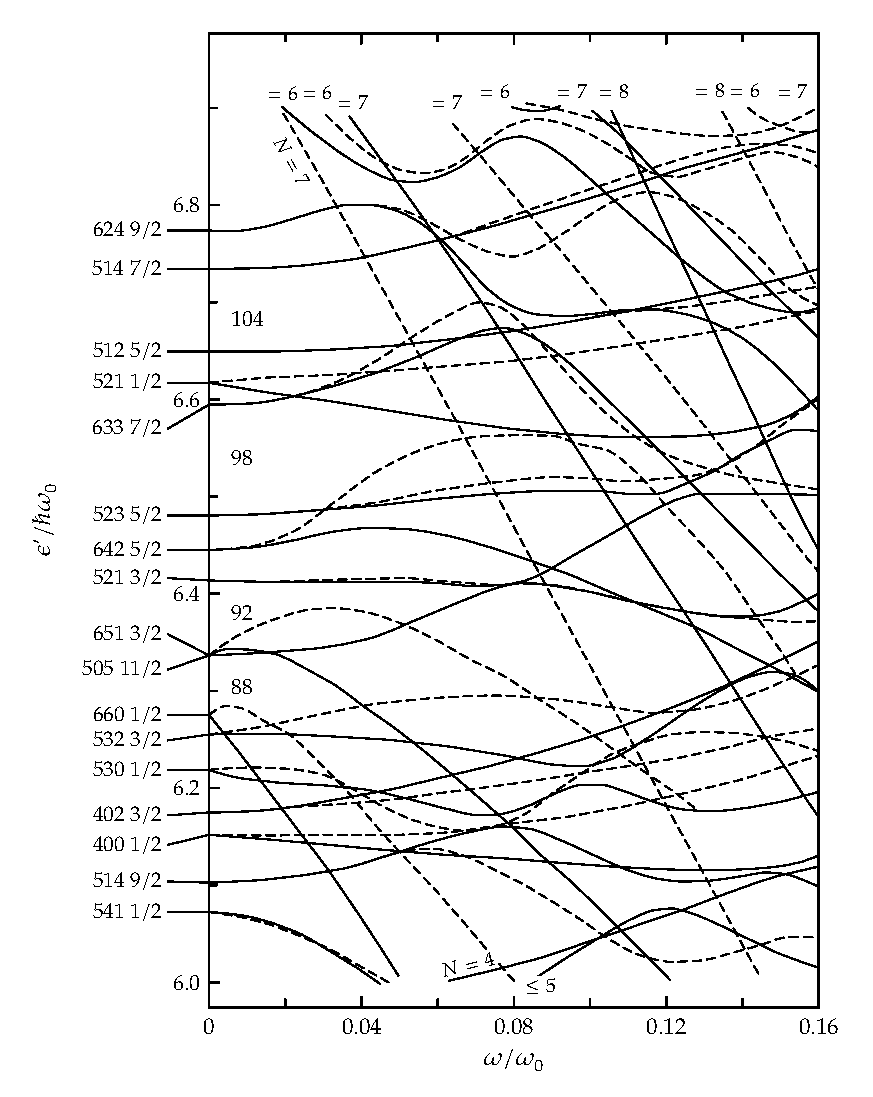
\includegraphics[width=0.75\textwidth]{pictures/3_15}
\par\end{centering}
\caption{\label{fig:3.15}在推引 Nilsson 势中单粒子能级作为 $\omega/\omega_{0}$ 的函数的定性行为。（引自
\cite{RNS78}。）}
\end{figure}


\subsection{高角动量下的形变势能面}

正如我们在 2.9 节中已经讨论过的，纯 Nilsson 模型既不能用于计算总能量，也不能用于计算大形变下的势能面形状，因为在该模型中能量的平均部分没有得到适宜的重现。因此，我们在此模型中仅计算形变能量的振荡部分（壳修正），并将光滑部分替换为相同形变下的液滴能量。

以同样的方式，我们可以计算在固定角动量 $I$ 下能量曲面作为形变的函数。对于椭球形状{[}由参数 $\beta$ 与 $\gamma$
表征，式 (1.88){]}，总能量由下式给出：

\begin{equation}
E(\beta,\gamma,I)=E_{\text{LDM}}(\beta,\gamma,I)+E_{\text{sh}}(\beta,\gamma,I)-\tilde{E}_{\text{sh}}(\beta,\gamma,I)\label{eq:3.123}
\end{equation}
此处 $E_{\text{LDM}}$ 是具有刚体转动惯量 $\mathcal{J}_{\text{rig}}(\beta,\gamma)$
的转动椭球的形变能，因为人们假定在高角动量下对关联可以忽略\footnote{事实上，级联 $\gamma$ 射线的重数测量表明，原子核在高自旋值下确实达到了刚体转动惯量 \cite{SBC76}。}。$E_{\text{sh}}$
是壳模型能量，通过对单粒子能量求和得到。$\tilde{E}_{\text{sh}}$ 是其平均部分，通过适宜的平滑程序算出（参见
2.9 节）。

存在两种途径从转动参考系中形变单粒子势的对角化导出这些物理量：或者在恒定频率 $\omega$ 下开展工作 \cite{NPF76}，或者在恒定角动量
$I$ 下开展工作 \cite{ALL76}。如果使用形变 Woods-Saxon 势（其平均转动惯量非常接近刚体值\footnote{Nilsson 势 (2.89) 中的 $\boldsymbol{l}^{2}$ 项是非局域的并对有效质量产生贡献。它给出的平均转动惯量比刚体值大约大
30–40\% \cite{Ty70,Ty71,BR71b,Je73}。人们曾采用定标程序来补偿这一效应 \cite{NTP77}。} \cite{BJ76b,NTP77}），这两种方法的结果完全一致。

若干研究小组沿着这一思路在周期表的许多区域展开了深入调查 \cite{BLL75,NP75,NPF76,ALL76,FDG76,NTP77}。在定性上他们发现了极为类似的结果：
\begin{enumerate}
\item[(i)] 对于稀土区开端的球形或弱形变核，其行为类似于经典液滴（图 1.18）：直到角动量 $I=50-70\,\hbar$，它们保持为扁椭球并绕对称轴旋转。在这一区域，转动是非集体的，人们预期出现晕阱（参见
3.4.7 节）。对于更高的 $I$ 值，它们迅速转变为三轴和长椭球形变（Jacobi 形状，参见 1.7 节）。这一转变对应于角动量的急剧剧增（“巨回弯”，giant
backbending），如\ref{fig:3.16} 所示。最终原子核发生裂变。
\item[(ii)] 稀土区中部的原子核在低 $I$ 值下从长椭球形状出发，并绕垂直于对称轴的轴旋转。随着转动的加剧，Coriolis 力使粒子顺排并驱动原子核走向非对称形状（三轴形变）。在许多计算中，人们甚至在
$I\sim50-70\,\hbar$ 处发现了向扁椭球形状的转变\footnote{在基于 Woods-Saxon 势的计算中 \cite{NTP77}，原子核不会达到如此极端的三轴形变，并且在尚未达到扁椭球形状之前就已经发生裂变。}，如\ref{fig:3.17}
所示。在极高角动量下，原子核再次变为三轴形变，并最终发生裂变。
\end{enumerate}
\begin{figure}[H]
\begin{centering}
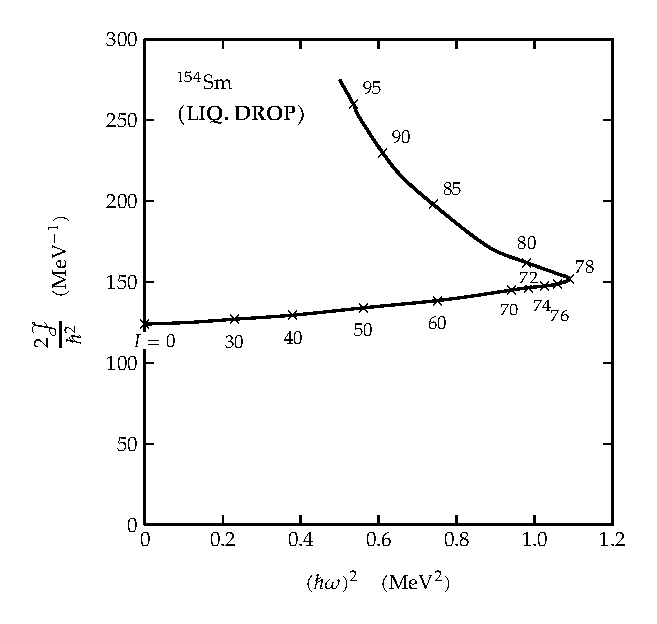
\includegraphics[width=0.75\textwidth]{pictures/3_16}
\par\end{centering}
\caption{\label{fig:3.16}根据转动液滴模型绘制的 $^{154}\text{Sm}$ 晕谱的回弯图。（引自 \cite{ALL76}。）}
\end{figure}

\begin{figure}[H]
\begin{centering}
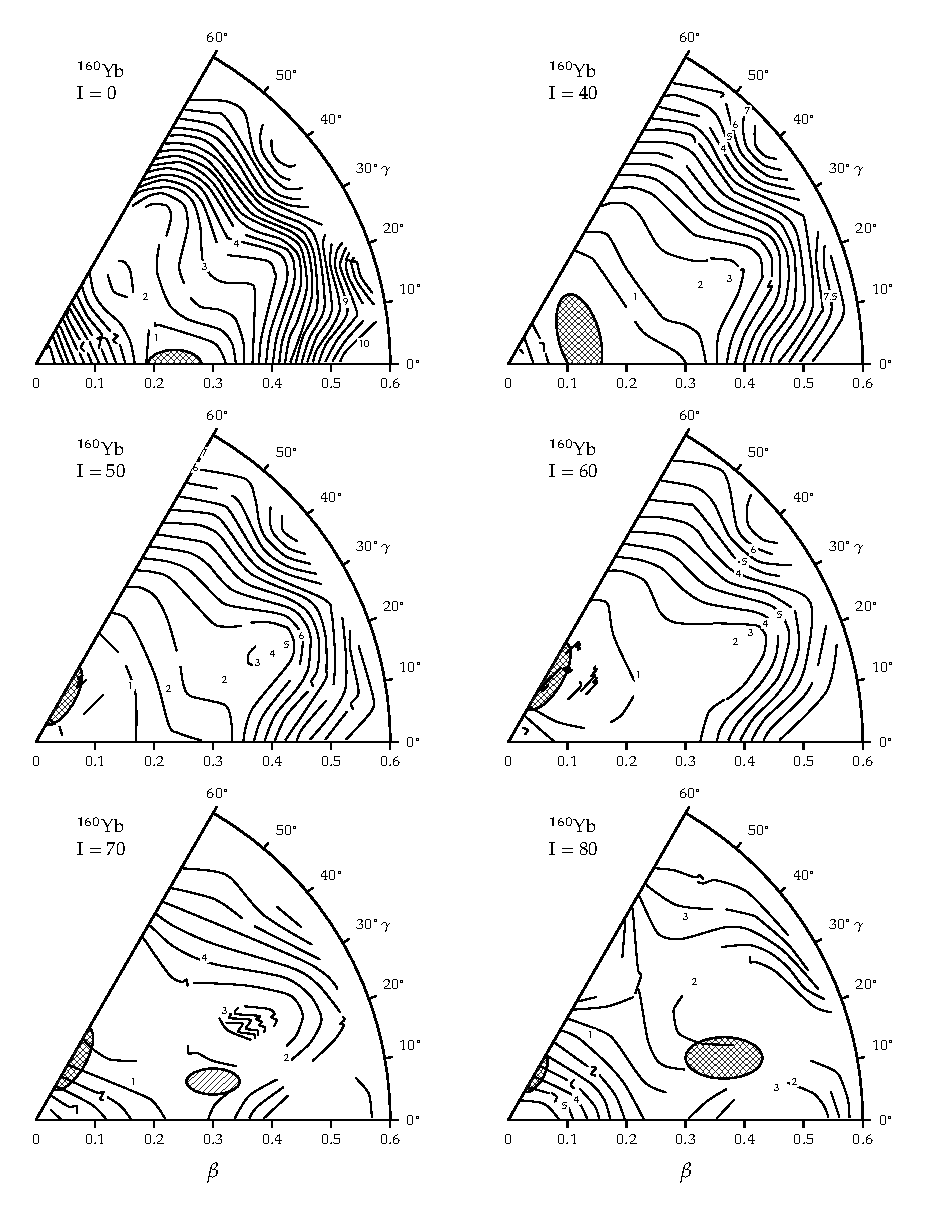
\includegraphics[width=0.75\textwidth]{pictures/3_17}
\par\end{centering}
\caption{\label{fig:3.17}计入壳修正后 $^{160}\text{Yb}$ 在 $(\beta,\gamma)$ 平面内的势能面随角动量的变化关系。（引自
\cite{ALL76}。请注意这些作者将 Hill-Wheeler 坐标 $\gamma$ 替换为 $-\gamma$。）}
\end{figure}

我们想在总结本小节时指出，此类计算仅能给出核多体系统在如此高角动量下行为的定性印象。只有对于极低激发能以及具有深势阱极小值的势能面，我们才能预期原子核具有确定的形变。一般而言，原子核将围绕这些极小值进行量子力学零点涨落，这应当由动力学理论予以描述（例如参见第
10 章）。

\subsection{绕对称轴的转动}

正如我们在前面几小节中所见，在元素周期表中存在一些区域，其中的原子核呈现绕对称轴“转动”。这尤其发生在每个主壳层的开端与末端。在每个壳层的开端，只有少数几个粒子位于或多或少为球形的核心之外。为了产生巨大的角动量，它们必须全部沿转动轴（$x$
轴）顺排；也就是说从经典角度来看，这些粒子必须在赤道平面内绕核运行，从而产生扁椭球的密度分布\footnote{在主壳层末端，类似的论据可以应用于空穴。此时我们最终得到绕长椭球密度分布对称轴的转动。在壳层中部存在许多形成长椭球形变的价粒子，通过少数几次顺排过程就极易产生大角动量，而不会对形变造成太剧烈的改变。}。

这种组态显然不是集体转动，因为其中仅涉及少数几个粒子。每一个单粒子波函数都是 $j_{x}$ 具有本征值 $\alpha_{i}$
的本征函数。总角动量沿对称轴方向的分量由下式给出：

\begin{equation}
\langle I_{x}\rangle=\sum^{A}_{i=1}\alpha_{i}\label{eq:3.124}
\end{equation}
为了增加角动量，我们必须改变形变势中的占据方式，将粒子从具有较低（例如负）$\alpha$ 值的能级提升到具有较高（正）$\alpha$
值的能级中。

在形式上，这同样可以通过绕对称轴的推引程序来实现。由于算符 $j_{x}$ 与 $h$ 对易，我们得到“转动参考系”中的单粒子能量：

\begin{equation}
\epsilon_{i}'=\epsilon_{i}-\omega\alpha_{i}\label{eq:3.125}
\end{equation}
其中 $\epsilon_{i}$ 是 $h$ 在非转动参考系中的本征值。作为 $\omega$ 的函数，它们是一组直线（\ref{fig:3.18}a），其斜率由下式给出：

\begin{equation}
\frac{\mathrm{d}\epsilon_{i}'}{\mathrm{d}\omega}=-\alpha_{i}\label{eq:3.126}
\end{equation}
在转动参考系中极小化能量的条件

\begin{equation}
E'=\sum^{A}_{i=1}(\epsilon_{i}-\omega\alpha_{i})\label{eq:3.127}
\end{equation}
保证了人们总是填充最低的能级 $\epsilon_{i}'$。随着频率 $\omega$ 的增加，我们因此获得了阶梯状递增的角动量（\ref{fig:3.18}b）。两阶之间的距离以及台阶的高度由能级
$\epsilon_{i}$ 之间的间距以及角动量数值 $\alpha_{i}$ 决定。因此，角动量随频率 $\omega$
的增加具有统计性的特征。转动惯量 $\mathcal{J}$ 仅在平均意义上被定义（\ref{fig:3.18}b 中的虚线）。

为了对该转动惯量的大小做出估计 \cite{Bo76b}，我们认识到\ref{fig:3.18}a 中的每一条线都具有斜率 $-\alpha_{i}$（取决于
$\alpha$ 的符号而上升或下降）。在 $\omega=0$ 处，能级 $\pm\alpha_{i}$ 全部成对占据，所得的总角动量为零。对于有限的
$\omega$，其中某些具有负 $\alpha$ 值的能级不再被占据，而其他具有正 $\alpha$ 值的下行能级则被重新占据。对于固定的
$\alpha$ 值（例如 $\alpha=1/2$），新占据能级的数目在平均意义上为 $\omega\alpha g(\alpha)$，其中
$g(\alpha)$ 是量子数为 $\alpha$ 的能级密度。因此在平均意义上我们获得角动量：

\begin{equation}
\langle I_{x}\rangle_{\text{av}}=\sum_{i}\alpha_{i}=\int\alpha\cdot\omega\alpha g(\alpha)\,\mathrm{d}\alpha=\omega\sum_{\alpha}\alpha^{2}g(\alpha)\label{eq:3.128}
\end{equation}
以及平均转动惯量：

\begin{equation}
\mathcal{J}_{\text{av}}=\sum_{\alpha}\alpha^{2}g(\alpha)\label{eq:3.129}
\end{equation}
在 Thomas-Fermi 近似下对该量的求值恰好给出刚体转动惯量的值。因此，绕对称轴的转动在整体上表现出与集体转动极其相似的宏观行为，尽管其微观内部结构截然不同。

\begin{figure}[H]
\begin{centering}
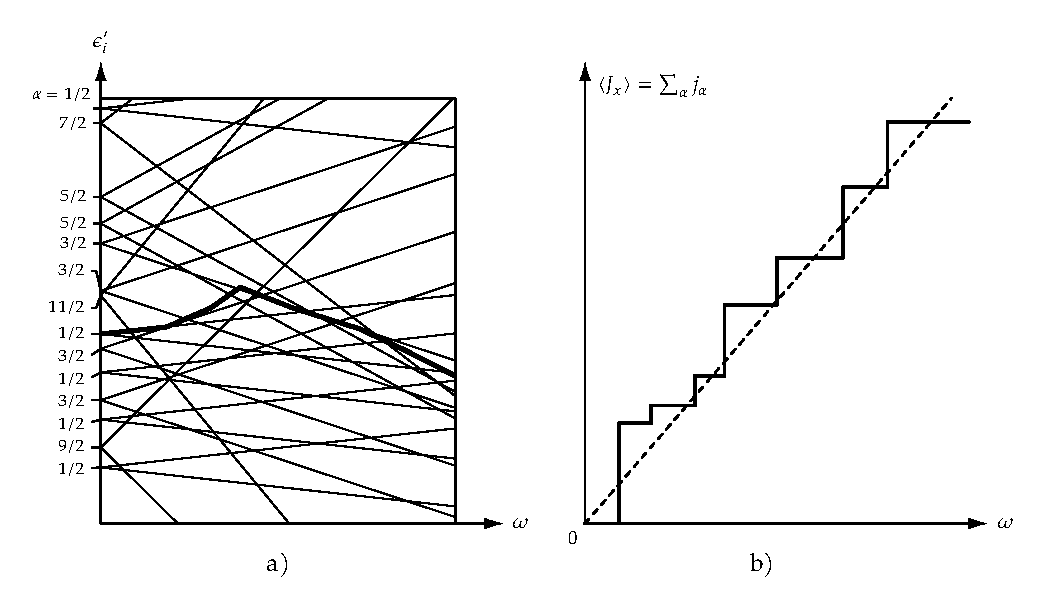
\includegraphics[width=0.75\textwidth]{pictures/3_18}
\par\end{centering}
\caption{\label{fig:3.18}(a) 式 (3.125) 中的本征值 $\epsilon_{i}'$ 作为推引频率的函数的示意图。(b)
随着 $\omega$ 的增加并通过总是占据 (a) 中的最低能级所获得的角动量 $\langle I_{x}\rangle$。}
\end{figure}


\subsection{晕阱}

由于在绕对称轴转动的情形下能级间距具有统计特征，人们预期存在\emph{晕阱}（yrast traps，即高自旋同核异能态）。它们被定义为不能发生快速
$\gamma$ 跃迁的晕态，由 Bohr 和 Mottelson \cite{BM74} 首次预测。

在转动势阱中始终从底部开始填充能级，随着角速度的增加，我们最终会获得角动量跨越若干个单位的跃变（参见\ref{fig:3.18}b）。这在非转动扁椭球形变
Nilsson 势阱的本征值 $\epsilon_{i}$ 作为沿对称轴角动量分量 $\alpha$ 的函数的表示中可以最直观地看清（\ref{fig:3.19}）。对于小形变，我们具有相当纯的
$j$ 组态。处于同一 $j$ 壳层能级的本征值 $\epsilon_{i}$ 近似落在抛物线上{[}参见\ref{eq:3.39}，我们只需将
$\Omega$ 替换为 $\alpha${]}。在扁椭球形变下（$\beta<0$），具有最高 $\alpha$ 值的态（即最大顺排的态）能量最低，因为它们在赤道面内的扁椭球密度分布与核心的扁椭球密度具有最大的重叠。

\begin{figure}[H]
\begin{centering}
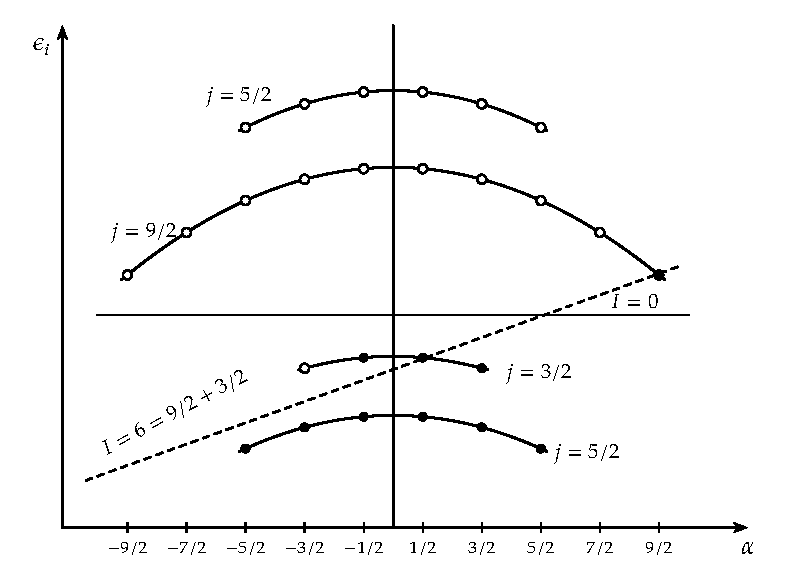
\includegraphics[width=0.75\textwidth]{pictures/3_19}
\par\end{centering}
\caption{\label{fig:3.19}扁椭球形变 Nilsson 势阱中单粒子能量 $\epsilon_{i}$ 作为 $\alpha$（$j_{x}$
的本征值）的函数的示意图，给出了 $I=0$ 处（实线）和 $I=6$ 处（虚线）的 Fermi 面。}
\end{figure}

在 $\omega=0$ 处，Fermi 面是一条水平线，位于其下的所有能级都被占据。在有限的 $\omega$ 值下，根据\ref{eq:3.125}，转动参考系中的
Fermi 面具有斜率 $\omega$。随着 $\omega$ 值的增加，具有负 $\alpha$ 值的能级被腾空，而具有正
$\alpha$ 值的能级被新占据。在\ref{fig:3.19} 中我们展示了发生 6 个单位角动量跃变的情形。晕线上的其余
$I$ 值可以通过构造相对于转动能面的粒子-空穴（ph）组态来获得。这通常伴随着能量的增加。因此，可能会出现晕线不再是 $I$
的单调递增函数的情况，某个具有 $I=I_{0}$ 的能级可能比邻近的 $I=I_{0}-1,I_{0}-2,\dots$ 能级具有更低的能量。此时快速的
$E1,E2,M1$ 或 $M2$ 跃迁（即低多极跃迁；参见附录 B）是不被允许的（所谓\emph{能量自旋阱}，energy
spin traps）。

即使不是这种情况，具有 $I_{0}-1,I_{0}-2$ 的态的内部结构可能与态 $I_{0}$ 的结构截然不同。此时跃迁矩阵元可能非常微小，态
$I_{0}$ 具有极长的寿命（所谓\emph{结构自旋阱}，structure spin traps）。典型的例子是：态 $I_{0}-1$
或 $I_{0}-2$ 只能通过从态 $I_{0}$ 进行 2p-2h 激发才能达到；或者 $\gamma$ 跃迁矩阵元受到单粒子波函数内禀选择定则的阻碍（例如
$l$ 禁戒的 $M1$ 跃迁，参见 2.7.2 节）。

若干研究小组通过在高角动量势能面上寻找绕对称轴转动的范例，并深入研究这些情形下的精细单粒子结构，从理论上探讨了晕阱存在的可能性 \cite{ALL76,CDS77,AK77,DNM77,PFL78,PTF78,AHL78,Ab78,MDN78}。在周期表中已经找到了一些应当预期存在晕阱的区域。它们主要是弱形变核，例如
Te、Ba、Ce、Sm、缺中子稀土同位素以及 Pb 区域的原子核。

在实验方面，人们很早就知道了球形核中具有大角动量和极长寿命的同核异能态。这些态具有相当纯的高 $j$ 壳层组态，对能量更低的其他态不存在低多极的允许
$\gamma$ 跃迁矩阵元。最著名的例子 \cite{PAG62} 是 $^{212}\text{Po}$ 中的 $18^{+}$
同核异能态，其寿命长达 45 秒，由顺排的 $(\pi h^{2}_{9/2})(\nu i_{11/2}g_{9/2})$ 组态构成。

在良好形变核中观测到了另一类高自旋同核异能态，通常称为 $K$-同核异能态，例如 $^{178}\text{Hf}$ 中的 $4\,\text{s}$
和 $31\,\text{y}$ 同核异能态，它们可以解释为 $K^{\pi}=8^{-}$ 和 $K^{\pi}=16^{+}$
的带头，其 $\gamma$ 衰变是 $K$ 禁戒的 \cite{HR68,KL77}。

最后，近年来在轻稀土区发现了由约 20 个相邻原子核组成的长寿命同核异能态“岛” \cite{PBB77}。它们很可能与扁椭球形变和“单粒子”转动相关联
\cite{AHL78}。

邻近 $^{208}\text{Pb}$ 的原子核性质通常是在带有剩余相互作用和适当角动量耦合技术的球形壳模型框架下进行研究的。由于这些组态相当纯净，此类计算能够以非凡的精度解释所测得的激发能
\cite{BBH77}。

在这一物理图像中，顺排的高自旋组态具有如此长寿命的物理原因与我们在绕对称轴转动模型中所解释的完全相同：两个自旋顺排的核子获得能量，是因为对于具有大空间重叠的波函数而言它们的剩余相互作用最大\footnote{该效应被称为 MONA 效应（通过顺排实现核波函数的最大重叠，Maximal Overlap of the Nuclear wave
function by Alignment \cite{FPD76}）。}（参见 4.4.8 节）。因此，这些高自旋能级的能量低于具有较小 $I$ 值的相邻态，快速 $\gamma$ 跃迁受到禁戒。在通过绕对称轴转动的平均场方法对这些核的描述中，相同的效应表现为（正如在\ref{fig:3.18}
中所讨论的）：具有最大 $\alpha$ 值和扁椭球密度分布的顺排能级，因其与扁椭球核心具有巨大的空间重叠，在能量上被大幅向下拉低。

这两种方法——基于角动量耦合技术的球形基底壳模型计算，以及略微形变势阱中的 cranking 计算——无疑是很难进行直接比较的。只要人们能够假定球形核心是惰性的，球形壳模型无疑要优秀得多（尽管它需要付出更多的计算努力），否则人们就必须考虑多粒子-多空穴组态。因此它仅限于幻数核的极其紧邻的区域。在另一方面，cranking
模型通过形变势阱来处理剩余相互作用，因而在广泛的原子核中极易处理。然而它仅允许给出非常定性的预言，因为它破坏了角动量守恒，并且仅在具有垂直于对称轴转动的良好形变核区域才具有微观推导基础（参见
11.4 节）。



\chapter{核力\label{chap:=006838=00529B}}

\section{引言}

到目前为止，我们只定性地考虑了核子间的作用力。我们用它们的某些性质——如短程性和饱和性——来解释液滴模型中的体积项和表面项。我们还假定它们给出了一个平均单粒子势。通过调整一些参数，我们能够复现大量的实验数据，这些唯象模型的成功使我们有信心进一步从更微观的角度研究核多体问题。另外，我们也希望应用现代多体理论的技术。

所有这些考虑的出发点显然是核子之间的两体相互作用。在这个概念中有三个基本假设：
\begin{enumerate}
\item 介子的动力学自由度可以忽略不计，原子核可以描述为$A$核子系统，其相互作用可以用势表示。
\item 相对论效应可以忽略不计。
\item 只有两体力是重要的。
\end{enumerate}
即使有了这些相当极端的假设，当我们试图按照我们讨论过的方式继续下去时，我们也会立即遇到两个困难：

第一，不存在从第一性原理导出核力的方法。虽然这在夸克和胶子规范场的现代理论中原则上是可能的，但在这方面的尝试还只是在起步阶段\cite{De78}。另一方面，从相互作用介子和核子的有效拉格朗日量出发的理论最近被证明是相当成功的（参见，例如，{[}CLL
73，LLR 75，DSB 77，Vi 78，Ho 80{]}）。这种核力的基本成分是$\pi$-核子耦合常数，这是从实验中得知的。当核子间距大于$0.8\,\text{fm}$时，这种核力没有自由参数，而从$0$到$0.8\,\text{fm}$的部分则由一个每个同位旋自由度上包含六个参数的唯象势表示，它最终很好地拟合了所测得的核子-核子相移。

迄今为止使用的核力几乎完全是唯象的（除了由单$\pi$介子交换产生的 Yukawa 势外；见下文），并包含多达约$50$个参数。这些核力很好的复现了实验上测得的相移。在这些核力的基础上，我们将在第4.2.2节非常简要地讨论如何应用多体理论的方法以定量的方式导出前面几章讨论的唯象性质。

然而，原子核理论中还有第二个困难。那就是从数值的观点来看，这些裸核力的行为非常病态。它们在短程内表现出很强的排斥行为（排斥芯）从而不能直接用一些多体方法来处理。例如，对于微扰论来说，这相互作用太强了，而对于自洽场方法（第五章）来说，排斥芯几乎是不可能处理的。事实上，核内的核子感受不到裸的核力，因为它们是在许多其他核子存在的情况下相互作用的，这允许我们引入所谓的有效核子-核子相互作用。这种相互作用表现得相当好，并允许我们应用通常的多体方法，如Hartree-Fock理论（第5章）。人们已经做了大量的工作，从裸核子-核子相互作用力导出这种有效相互作用。在4.3节我们讨论了为实现这一目标所采用的基本思想。迄今为止，人们对这些有效核力的性质和结构已经有了大量的了解。然而，为了定量地再现实验数据，人们仍然需要唯象的调整这些参数，从这个角度来看，这一理论还不是很令人满意。

在大多数所谓的原子核微观描述中，人们使用唯象的有效核力，这些有效核力是基于这些考虑而构建的，但仍然有一些可调节的用来适应实验数据的参数。

在这一章我们并不想尝试去推导裸核力\cite{BJ76a}。在第二节我们将会讨论裸核力有的一些对称性，这使得我们可以推导一些结论。第三节我们简要介绍了有效相互作用的微观描述，讨论了它们的性质和应用领域。第四节介绍了一些用于描述一个给定平均势中运动核子间的剩余相互作用的唯象势。

需要强调的是，在这一章中我们只讨论核力，而库仑力必须单独讨论。当需要与实验数据进行比较时，必须首先减去库仑效应。

\section{裸核力\label{sec:=0088F8=006838=00529B}}

\subsection{两体力的一般性质}

量子力学中最一般的两体相互作用$V$可以由其夹在两粒子态（坐标表象下是$|\boldsymbol{r}_{1},s_{1},t_{1};\boldsymbol{r}_{2},s_{2},t_{2}\rangle$，这里$s_{i}=\pm\frac{1}{2}$是自旋，$t_{i}=\pm\frac{1}{2}$是同位旋）间得到的矩阵元完全确定：
\[
\langle\boldsymbol{r}^{\prime}_{1}s^{\prime}_{1}t^{\prime}_{1}\boldsymbol{r}^{\prime}_{2}s^{\prime}_{2}t^{\prime}_{2}|V|\boldsymbol{r}_{1}s_{1}t_{1}\boldsymbol{r}_{2}s_{2}t_{2}\rangle
\]

两粒子态$|\boldsymbol{r}_{1},s_{1},t_{1};\boldsymbol{r}_{2},s_{2},t_{2}\rangle$的空间是空间波函数$|\boldsymbol{r}_{1}\rangle$和$|\boldsymbol{r}_{2}\rangle$，自旋和同位旋态矢$|s_{1}\rangle,|s_{2}\rangle$和$|t_{1},t_{2}\rangle$的直积。由于自旋空间的任意算符都可以表示为Pauli矩阵$\sigma_{1}$，$\sigma_{2}$，$\sigma_{3}$和单位矩阵$\sigma_{0}$的线性组合
\begin{comment}
这一结论依赖于厄米性，而本书中后面又把厄米性当做单独的对称性，是一种逻辑混乱。
\end{comment}
，因此最一般的形式是：
\begin{equation}
V=\sum^{3}_{i,j=0}V_{ij}\sigma^{(1)}_{i}\sigma^{(2)}_{j}\label{eq:general V in spin space}
\end{equation}

类似地，$V_{ij}$也这么依赖于同位旋算符$\boldsymbol{\tau}^{(1)}$和$\boldsymbol{\tau}^{(2)}$。除了这一同位旋依赖性，坐标空间的$V_{ij}$是积分算符：
\begin{equation}
V|\boldsymbol{r}_{1}\boldsymbol{r}_{2}\rangle=\int V(\boldsymbol{r}^{\prime}_{1},\boldsymbol{r}^{\prime}_{2},\boldsymbol{r}_{1},\boldsymbol{r}_{2})|\boldsymbol{r}^{\prime}_{1}\boldsymbol{r}^{\prime}_{2}\rangle\,\mathrm{d}^{3}\boldsymbol{r}^{\prime}_{1}\mathrm{d}^{3}\boldsymbol{r}^{\prime}_{2}\label{eq:V in coordinate space}
\end{equation}

特殊情况下，$V(\boldsymbol{r}^{\prime}_{1},\boldsymbol{r}^{\prime}_{2},\boldsymbol{r}_{1},\boldsymbol{r}_{2})$具有如下形式：
\[
V(\boldsymbol{r}_{1},\boldsymbol{r}_{2},\boldsymbol{r}^{\prime}_{1},\boldsymbol{r}^{\prime}_{2})=\delta(\boldsymbol{r}_{1}-\boldsymbol{r}^{\prime}_{1})\delta(\boldsymbol{r}_{2}-\boldsymbol{r}^{\prime}_{2})V(\boldsymbol{r}_{1},\boldsymbol{r}_{2})
\]

这时$V$被称为局域势，我们有：
\[
V|\boldsymbol{r}_{1}\boldsymbol{r}_{2}\rangle=V(\boldsymbol{r}_{1},\boldsymbol{r}_{2})|\boldsymbol{r}_{1}\boldsymbol{r}_{2}\rangle
\]

在这种情况下，两粒子相互作用仅仅依赖于$\boldsymbol{r}_{1}$和$\boldsymbol{r}_{2}$（当然也依赖于自旋和同位旋）。它并不依赖于如粒子的速度这样的量。

我们需要说明，一般来讲，非局域的势是速度依赖的。我们把$|\boldsymbol{r}^{\prime}_{1}\boldsymbol{r}^{\prime}_{2}\rangle$展开\footnote{这里$:\mathrel{}:$是正规序，意思是说$\partial/\partial\boldsymbol{r}_{i}$不作用到指数展开项的$\boldsymbol{r}_{i}$上。}：

\begin{align*}
|\boldsymbol{r}^{\prime}_{1},\boldsymbol{r}^{\prime}_{2}\rangle & =|\boldsymbol{r}_{1}\boldsymbol{r}_{2}\rangle+(\boldsymbol{r}^{\prime}_{1}-\boldsymbol{r}_{1})\frac{\partial}{\partial\boldsymbol{r}_{1}}|\boldsymbol{r}_{1}\boldsymbol{r}_{2}\rangle+(\boldsymbol{r}^{\prime}_{2}-\boldsymbol{r}_{2})\frac{\partial}{\partial\boldsymbol{r}_{2}}|\boldsymbol{r}_{1}\boldsymbol{r}_{2}\rangle+\dots\\
 & =:\mathrel{\exp\left((\boldsymbol{r}^{\prime}_{1}-\boldsymbol{r}_{1})\frac{\partial}{\partial\boldsymbol{r}_{1}}+(\boldsymbol{r}^{\prime}_{2}-\boldsymbol{r}_{2})\frac{\partial}{\partial\boldsymbol{r}_{2}}\right)}:|\boldsymbol{r}_{1}\boldsymbol{r}_{2}\rangle
\end{align*}

由\ref{eq:V in coordinate space}可以得到：
\begin{align*}
V|\boldsymbol{r}_{1}\boldsymbol{r}_{2}\rangle & =\int V(\boldsymbol{r}^{\prime}_{1},\boldsymbol{r}^{\prime}_{2},\boldsymbol{r}_{1},\boldsymbol{r}_{2})\exp\left(\frac{\mathrm{i}}{\hbar}(\boldsymbol{r}^{\prime}_{1}-\boldsymbol{r}_{1})\boldsymbol{p}_{1}+\frac{\mathrm{i}}{\hbar}(\boldsymbol{r}^{\prime}_{2}-\boldsymbol{r}_{2})\boldsymbol{p}_{2}\right)|\boldsymbol{r}_{1}\boldsymbol{r}_{2}\rangle\,\mathrm{d}^{3}\boldsymbol{r}^{\prime}_{1}\mathrm{d}^{3}\boldsymbol{r}^{\prime}_{2}\\
 & =\tilde{V}(\boldsymbol{r}_{1},\boldsymbol{p}_{1},\boldsymbol{r}_{2},\boldsymbol{p}_{2})|\boldsymbol{r}_{1}\boldsymbol{r}_{2}\rangle
\end{align*}

这意味着最一般的势可以用\ref{eq:general V in spin space}表示，里面的$V_{ij}$在坐标空间中具有上式的形式（为了简化我们忽略了同位旋依赖性）。

接下来我们讨论核力$V(1,2)=V(\boldsymbol{r}_{1},\boldsymbol{p}_{1},\boldsymbol{\sigma}^{(1)},\boldsymbol{\tau}^{(1)},\boldsymbol{r}_{2},\boldsymbol{p}_{2},\boldsymbol{\sigma}^{(2)},\boldsymbol{\tau}^{(2)})$的对称性。通过给定一系列的对称性，这一普适的函数形式会被限制。

这里我们给定了八种对称性：
\begin{enumerate}
\item 厄米性
\item 置换对称性
\[
V(1,2)=V(2,1)
\]

这一性质和两粒子波函数的对称性相关。由于核子是费米子，它们具有反对称性。例如，如果我们写出一个坐标空间，自旋空间和同位旋空间的直积波函数：
\[
\langle\boldsymbol{r}_{1}s_{1}t_{1},\boldsymbol{r}_{2}s_{2}t_{2}|12\rangle=\varphi(\boldsymbol{r}_{1},\boldsymbol{r}_{2})\chi(s_{1},s_{2})\zeta(t_{1},t_{2})
\]

我们有四种符合泡利原理的组合，它们可以通过坐标空间和自旋部分的对称性来标记\ref{tab:=004E24=007C92=005B50=006001=005BF9=0079F0=006027=007684=005206=007C7B}，在每种情况下，同位旋分量都是通过总波函数的反对称性来确定的。
\begin{table}[H]
\begin{centering}
\caption{\label{tab:=004E24=007C92=005B50=006001=005BF9=0079F0=006027=007684=005206=007C7B}两粒子态对称性的分类}
\par\end{centering}
\centering{}%
\begin{tabular}{|c|c|c|c|}
\hline 
$\varphi$ & $\chi$ & 缩写 & $\zeta$\tabularnewline
\hline 
\hline 
偶 & 单态 & es & $+$\tabularnewline
\hline 
偶 & 三重态 & et & $-$\tabularnewline
\hline 
奇 & 单态 & os & $-$\tabularnewline
\hline 
奇 & 三重态 & ot & $+$\tabularnewline
\hline 
\end{tabular}
\end{table}

\item 平移不变性。核力只依赖于相对坐标：
\[
V(1,2)=V(\boldsymbol{r},\boldsymbol{p}_{1},\boldsymbol{\sigma}^{(1)},\boldsymbol{\tau}^{(1)},\boldsymbol{p}_{2},\boldsymbol{\sigma}^{(2)},\boldsymbol{\tau}^{(2)})
\]
\item 伽利略不变性。核力在惯性参考系之间的变换下不变，即只依赖于相对动量$\boldsymbol{p}=\frac{1}{2}(\boldsymbol{p}_{1}-\boldsymbol{p}_{2})$：
\[
V(1,2)=V(\boldsymbol{r},\boldsymbol{p},\boldsymbol{\sigma}^{(1)},\boldsymbol{\tau}^{(1)},\boldsymbol{\sigma}^{(2)},\boldsymbol{\tau}^{(2)})
\]
\item 空间反演不变性。和弱相互作用不同，强相互作用是宇称守恒的：
\[
V(\boldsymbol{r},\boldsymbol{p},\boldsymbol{\sigma}^{(1)},\boldsymbol{\tau}^{(1)},\boldsymbol{\sigma}^{(2)},\boldsymbol{\tau}^{(2)})=V(-\boldsymbol{r},-\boldsymbol{p},\boldsymbol{\sigma}^{(1)},\boldsymbol{\tau}^{(1)},\boldsymbol{\sigma}^{(2)},\boldsymbol{\tau}^{(2)})
\]
\item 时间反演不变性。它保证了运动方程不依赖于时间演化的方向（细节参考\cite{Me61}）。
\[
V(\boldsymbol{r},\boldsymbol{p},\boldsymbol{\sigma}^{(1)},\boldsymbol{\tau}^{(1)},\boldsymbol{\sigma}^{(2)},\boldsymbol{\tau}^{(2)})=V(\boldsymbol{r},-\boldsymbol{p},-\boldsymbol{\sigma}^{(1)},\boldsymbol{\tau}^{(1)},-\boldsymbol{\sigma}^{(2)},\boldsymbol{\tau}^{(2)})
\]
\item 空间转动不变性。三维空间转动不仅仅作用在$\boldsymbol{r}$和$\boldsymbol{p}$上，也作用在自旋矩阵$\boldsymbol{\sigma}=2\cdot\boldsymbol{s}$上。算符$V$在自旋空间必须具有\ref{eq:general V in spin space}的形式。它必须在空间转动下是标量，这意味着$V_{00}$必须是个标量。我们从$\boldsymbol{r}$和$\boldsymbol{p}$可以构建三个独立的标量$r^{2}$，$p^{2}$和$\boldsymbol{r}\cdot\boldsymbol{p}+\boldsymbol{p}\cdot\boldsymbol{r}$。由于时间反演不变性，后一个表达式只能以二次的形式出现。因此一种更方便的方法是把$(\boldsymbol{r}\cdot\boldsymbol{p}+\boldsymbol{p}\cdot\boldsymbol{r})^{2}$用$r^{2}$，$p^{2}$和$L^{2}=(\boldsymbol{r}\times\boldsymbol{p})^{2}$表示出来。$V_{00}$可以写成$r^{2}$，$p^{2}$和$L^{2}$的函数。由于置换对称性和空间反演不变性我们发现：
\[
V(\boldsymbol{r},\boldsymbol{p},\boldsymbol{\sigma}^{(1)},\boldsymbol{\sigma}^{(2)})=V(\boldsymbol{r},\boldsymbol{p},\boldsymbol{\sigma}^{(2)},\boldsymbol{\sigma}^{(1)})
\]

因此\ref{eq:general V in spin space}中的线性项只依赖于：
\[
\boldsymbol{S}=\frac{1}{2}(\boldsymbol{\sigma}^{(1)}+\boldsymbol{\sigma}^{(2)})
\]

为了形成一个标量，$\boldsymbol{S}$必须和一个矢量相乘，此外还要考虑空间反演不变性，只有$\boldsymbol{L}$满足这一要求：
\[
\boldsymbol{L}\cdot\boldsymbol{S}=\frac{1}{2}\boldsymbol{L}\cdot(\boldsymbol{\sigma}^{(1)}+\boldsymbol{\sigma}^{(2)})
\]

\ref{eq:general V in spin space}中的二次项形成了一个张量，。它可以分解成一个标量$\boldsymbol{\sigma}^{(1)}\cdot\boldsymbol{\sigma}^{(2)}$，一个矢量$\boldsymbol{\sigma}^{(1)}\times\boldsymbol{\sigma}^{(2)}$，一个无迹对称张量$(\sigma^{(1)}_{i}\sigma^{(2)}_{k}+\sigma^{(1)}_{k}\sigma^{(2)}_{i})(1-\frac{1}{3}\delta_{ik})$。根据Okubo和Marshak\cite{OM58}的研究，$\boldsymbol{\sigma}^{(1)}\times\boldsymbol{\sigma}^{(2)}$不能出现，所有可能的组合是：
\[
\boldsymbol{\sigma}^{(1)}\cdot\boldsymbol{\sigma}^{(2)},(\boldsymbol{r}\cdot\boldsymbol{\sigma}^{(1)})(\boldsymbol{r}\cdot\boldsymbol{\sigma}^{(2)}),(\boldsymbol{p}\cdot\boldsymbol{\sigma}^{(1)})(\boldsymbol{p}\cdot\boldsymbol{\sigma}^{(2)}),(\boldsymbol{L}\cdot\boldsymbol{\sigma}^{(2)})(\boldsymbol{L}\cdot\boldsymbol{\sigma}^{(2)})+(\boldsymbol{L}\cdot\boldsymbol{\sigma}^{(2)})(\boldsymbol{L}\cdot\boldsymbol{\sigma}^{(1)})
\]

所有这些项都可以与$r^{2}$，$p^{2}$和$L^{2}$的任意函数相乘。
\item 同位旋空间的转动不变性。在同位旋的框架下，质子和中子被视为一种可以形成同位旋$\frac{1}{2}$双重态的基本粒子。转动群的二维表示即可刻画它们所有的变换性质。同位旋空间的转动（只要它们不是沿着第三个轴
\begin{comment}
这句话是什么意思？
\end{comment}
）产生了质子中子的混合态。核力的转动不变性因此意味着电荷无关性，也就是质子质子相互作用和中子中子相互作用相同。这可以从核子核子散射实验和镜像核（例如$\text{He}^{3}$和$\text{H}^{3}$）的性质得出。数学上讲，这意味着核力$V(1,2)$和总同位旋算符$\boldsymbol{T}=\boldsymbol{t}_{1}+\boldsymbol{t}_{2}$交换。因此本征态可以通过$T^{2}$，$T_{3}$对应的本征值为$T=0$，$T_{3}=0$和$T=1$，$T_{3}=-1,0,+1$的态（同位旋单重态和三重态）构造出来。电荷无关性意味着$T^{2}$与核力算符对易。因此，$T=1$态的相互作用（pp，nn或者对称的pn态）必须是一样的。然而，$T=0$的态可能是不同的。

同位旋矩阵$\boldsymbol{\tau}=(\tau_{1},\tau_{2},\tau_{3})$的形式和通常的自旋矩阵相同。由于同位旋空间没有其它矢量，因此仅有的同位旋转动不变的粒子1和2的组合是：
\[
V_{0}+V_{\tau}\boldsymbol{\tau}^{(1)}\cdot\boldsymbol{\tau}^{(2)}
\]

正如我们已经讨论的$V_{0}$和$V_{\tau}$依赖于剩余的坐标例如$\boldsymbol{r}$，$\boldsymbol{p}$，$\boldsymbol{\sigma}_{1}$，$\boldsymbol{\sigma}_{2}$。
\end{enumerate}
不是所有对称性允许的组合都被用来描述核力，我们这里只涉及一些重要的项：
\begin{enumerate}
\item 局域的，即不依赖于速度的势中，中心力是最重要的。它仅仅依赖于核子间的距离$r$：
\begin{equation}
V_{\text{C}}(1,2)=V_{0}(r)+V_{\sigma}(r)\boldsymbol{\sigma}^{(1)}\cdot\boldsymbol{\sigma}^{(2)}+V_{\tau}(r)\boldsymbol{\tau}^{(1)}\cdot\boldsymbol{\tau}^{(2)}+V_{\sigma\tau}(r)(\boldsymbol{\sigma}^{(1)}\cdot\boldsymbol{\sigma}^{(2)})(\boldsymbol{\tau}^{(1)}\cdot\boldsymbol{\tau}^{(2)})\label{eq:center force}
\end{equation}
\item 剩余的局域势是张量力：
\[
V_{T}(1,2)=[V_{T_{0}}(r)+V_{T}(r)\boldsymbol{\tau}^{(1)}\cdot\boldsymbol{\tau}^{(2)}]\boldsymbol{S}_{12}
\]

这里：
\[
S_{12}=\frac{3}{r^{2}}(\boldsymbol{\sigma}^{(1)}\cdot\boldsymbol{r})(\boldsymbol{\sigma}^{(2)}\cdot\boldsymbol{r})-\boldsymbol{\sigma}^{(1)}\cdot\boldsymbol{\sigma}^{(2)}
\]

$-\boldsymbol{\sigma}^{(1)}\cdot\boldsymbol{\sigma}^{(2)}$这一项添加是为了保证$V_{T}(1,2)$对所有的方向积分为零：
\[
\int V_{T}(1,2)\,\mathrm{d}\Omega=0\quad\text{这里}\boldsymbol{r}=(r,\Omega)
\]

实验上关于核子核子间张量力存在的证据是氚核的四极矩，这是不能被单纯的中心力解释的。
\item 最重要的非局域势是两体自旋轨道相互作用：
\[
V_{LS}=V_{LS}(r)\boldsymbol{L}\cdot\boldsymbol{S}
\]

正如我们在第五章将会看到的，这样的一个两体自旋轨道耦合项导致了平均单粒子势中的单体自旋轨道耦合项，可以被用来解释原子核中的幻数。
\item 有时候我们也用二阶的自旋轨道相互作用：
\[
V_{LL}=V_{LL}(r)\left\{ (\boldsymbol{\sigma}^{(1)}\cdot\boldsymbol{\sigma}^{(2)})L^{2}-\frac{1}{2}\left[(\boldsymbol{\sigma}^{(1)}\cdot\boldsymbol{L})(\boldsymbol{\sigma}^{(2)}\cdot\boldsymbol{L})+(\boldsymbol{\sigma}^{(2)}\cdot\boldsymbol{L})(\boldsymbol{\sigma}^{(1)}\cdot\boldsymbol{L})\right]\right\} 
\]
\end{enumerate}

\subsection{核力的结构}

中心力是核子核子相互作用中最重要的部分。它也可以用一些交换或者投影算符来表示。

下面的算符可以交换波函数中的自旋和同位旋坐标：
\begin{align*}
P^{\sigma} & =\frac{1}{2}(1+\boldsymbol{\sigma}^{(1)}\cdot\boldsymbol{\sigma}^{(2)})\\
P^{\tau} & =\frac{1}{2}(1+\boldsymbol{\tau}^{(1)}\cdot\boldsymbol{\tau}^{(2)})
\end{align*}

我们把$P^{\sigma}$作用到波函数上即可得到：

\[
P^{\sigma}\varphi(\boldsymbol{r}_{1},\boldsymbol{r}_{2})\chi(s_{1},s_{2})\zeta(t_{1},t_{2})=\varphi(\boldsymbol{r}_{1},\boldsymbol{r}_{2})\chi(s_{2},s_{1})\zeta(t_{1},t_{2})
\]

这可以很容易的通过总自旋算符$\boldsymbol{S}$算符理解。$S^{2}$算符的本征态是单态或者三重态：

\[
P^{\sigma}=\frac{1}{2}[1+2(S^{2}-s^{(1)2}-s^{(2)2})]=S(S+1)-1=\begin{cases}
1 & \text{三重态}\\
-1 & \text{单态 }
\end{cases}
\]

我们也可以定义一个算符$P^{r}$交换粒子的空间坐标$\boldsymbol{r}_{1}$和$\boldsymbol{r}_{2}$。

\footnote{这一算符可以在坐标空间用一个非局域的算符表示：
\[
V(\boldsymbol{r})P^{r}\psi(\boldsymbol{r}_{1},\boldsymbol{r}_{2})=\int V(\boldsymbol{r}_{1}-\boldsymbol{r}_{2})\delta(\boldsymbol{r}^{\prime}_{1}-\boldsymbol{r}_{2})\delta(\boldsymbol{r}^{\prime}_{2}-\boldsymbol{r}_{1})\psi(\boldsymbol{r}^{\prime}_{1},\boldsymbol{r}^{\prime}_{2})\,\mathrm{d}^{3}\boldsymbol{r}^{\prime}_{1}\mathrm{d}^{3}\boldsymbol{r}^{\prime}_{2}
\]

在这种意义下Wigner力是局域的。}

\begin{comment}
求求了不要写这么愚蠢的形式，用Dirac符号表示算符不好吗。
\end{comment}
\begin{comment}
什么意义下是局域的？
\end{comment}
由于波函数在置换粒子1和粒子2的所有坐标下反对称，Pauli规则可以写为：

\[
P^{r}P^{\sigma}P^{\tau}=-1
\]

我么因此可以把算符$P^{\tau}$表示成$-P^{r}P^{\sigma}$，同时省去\ref{eq:center force}中的$\boldsymbol{\sigma}^{(1)}\cdot\boldsymbol{\sigma}^{(2)}$和$\boldsymbol{\tau}^{(1)}\cdot\boldsymbol{\tau}^{(2)}$。

最终我们得到：
\[
V_{\text{C}}=V_{\text{W}}(r)+V_{\text{M}}(r)P^{r}+V_{\text{B}}(r)P^{\sigma}+V_{\text{H}}(r)P^{r}P^{\sigma}
\]

有如下关系：

\begin{align*}
V_{\text{W}} & =V_{0}-V_{\sigma}-V_{\tau}+V_{\sigma\tau} &  & (\text{Wigner力})\\
V_{\text{M}} & =-4V_{\sigma\tau} &  & (\text{Majorana力})\\
V_{\text{B}} & =2V_{\sigma}-2V_{\sigma\tau} &  & (\text{Bartlett力})\\
V_{\text{H}} & =-2V_{\tau}+2V_{\sigma\tau} &  & (\text{Heisenberg力})
\end{align*}

这些核力不同组分的命名要追溯到20世纪30年代，当时第一批核模型被提出，核力的饱和性被交换项解释，而无需引入一个强排斥芯（关于这些工作的历史，可以参考\cite{Br65a}）。

第三种表示中心力的方式是利用投影算符：
\begin{align*}
\Pi^{\sigma}_{\text{s}} & =\frac{1}{2}(1-P^{\sigma}) & \Pi^{\sigma}_{\text{t}} & =\frac{1}{2}(1+P^{\sigma})\\
\Pi^{\tau}_{\text{s}} & =\frac{1}{2}(1-P^{\tau}) & \Pi^{\tau}_{\text{t}} & =\frac{1}{2}(1+P^{\tau})\\
\Pi^{r}_{\text{o}} & =\frac{1}{2}(1-P^{r}) & \Pi^{r}_{\text{e}} & =\frac{1}{2}(1+P^{r})
\end{align*}

这些是投影算符（$P^{2}=P$，$P^{\dagger}=P$），分别投影到\ref{tab:=004E24=007C92=005B50=006001=005BF9=0079F0=006027=007684=005206=007C7B}中的两体波函数的单态（s）和三重态（t），或者偶态（e）和奇态（o）。我们可以把交换算符$P^{\sigma}$，$P^{r}$用相应的投影算符展开得到：
\[
V(1,2)=V_{\text{et}}(r)\Pi^{r}_{\text{e}}\Pi^{\sigma}_{\text{t}}+V_{\text{es}}(r)\Pi^{r}_{\text{e}}\Pi^{\sigma}_{\text{s}}+V_{\text{ot}}(r)\Pi^{r}_{\text{o}}\Pi^{\sigma}_{\text{t}}+V_{\text{os}}(r)\Pi^{r}_{\text{o}}\Pi^{\sigma}_{\text{s}}
\]

这个表示在实际应用中非常有用。例如，在质子质子散射实验中，我们只有同位旋三重态（只有es和ot是重要的）。\ref{tab:=004E2D=005FC3=00529B=004E0D=00540C=008868=00793A=004E4B=0095F4=007684=005173=007CFB}展示了这些函数如何用其它表示方式中的系数表示出来
\begin{comment}
这里按照我自己的理解翻译的，此外，表格中的第三列中每个下标都被我删去了一个$0$，我没有看出这个$0$的意义。
\end{comment}
。

\begin{table}[H]
\begin{centering}
\caption{\label{tab:=004E2D=005FC3=00529B=004E0D=00540C=008868=00793A=004E4B=0095F4=007684=005173=007CFB}中心力不同表示之间的关系}
\par\end{centering}
\centering{}%
\begin{tabular}{|c|c|c|c|c|c|}
\hline 
$\boldsymbol{\sigma}^{(1)}\boldsymbol{\sigma}^{(2)}$ & $\boldsymbol{\tau}^{(1)}\boldsymbol{\tau}^{(2)}$ & $V(\boldsymbol{\sigma}^{(1)}\boldsymbol{\sigma}^{(2)},\boldsymbol{\tau}^{(1)}\boldsymbol{\tau}^{(2)})$ & $V(P^{r},P^{\sigma})$ & $V(\Pi^{r},\Pi^{\sigma})$ & $|12\rangle$\tabularnewline
\hline 
\hline 
1 & -3 & $V_{0}+V_{\sigma}-3V_{\tau}-3V_{\sigma\tau}$ & $V_{\text{W}}+V_{\text{M}}+V_{\text{B}}+V_{\text{H}}$ & $V_{\text{et}}$ & $|\text{et}\rangle$\tabularnewline
\hline 
-3 & 1 & $V_{0}-3V_{\sigma}+V_{\tau}-3V_{\sigma\tau}$ & $V_{\text{W}}+V_{\text{M}}-V_{\text{B}}-V_{\text{H}}$ & $V_{\text{es}}$ & $|\text{es}\rangle$\tabularnewline
\hline 
1 & 1 & $V_{0}+V_{\sigma}+V_{\tau}+V_{\sigma\tau}$ & $V_{\text{W}}-V_{\text{M}}+V_{\text{B}}-V_{\text{H}}$ & $V_{\text{ot}}$ & $|\text{ot}\rangle$\tabularnewline
\hline 
-3 & -3 & $V_{0}-3V_{\sigma}-3V_{\tau}+9V_{\sigma\tau}$ & $V_{\text{W}}-V_{\text{M}}-V_{\text{B}}+V_{\text{H}}$ & $V_{\text{os}}$ & $|\text{os}\rangle$ \tabularnewline
\hline 
\end{tabular}
\end{table}

函数$V$的径向依赖无法从对称性得出。1937年，汤川用介子场解释了核力的起源。核子通过交换一个或多个介子相互作用。最简单的形式是单$\pi$介子交换项（OPEP）。它具有
Yukawa 势形式的径向依赖 \cite{Yu35}：
\[
V_{\text{Y}}(r)=\frac{\mathrm{e}^{-\mu r}}{\mu r}
\]

这里$1/\mu=\hbar/m_{\pi}c$是$\pi$介子的康普顿波长。单$\pi$介子交换项的渐进形式由$\pi$介子的性质和它与核子的耦合强度$g^{2}/\hbar c\simeq0.081$唯一确定：
\[
V^{\text{OPEP}}=\frac{g^{2}}{3\hbar c}m_{\pi}c^{2}\frac{\mathrm{e}^{-\mu r}}{\mu r}(\boldsymbol{\tau}^{(1)}\cdot\boldsymbol{\tau}^{(2)})\left\{ \boldsymbol{\sigma}^{(1)}\cdot\boldsymbol{\sigma}^{(2)}+\left[1+3\frac{1}{\mu r}+3\left(\frac{1}{\mu r}\right)^{2}\right]S_{12}\right\} 
\]

核子核子散射数据的相移分析表明单$\pi$介子交换势很好的复现了大轨道量子数即$L\gg6$的情况下的相移\cite{Br67b}。由于这些高分波仅仅只能感受到核力的长程部分（$r\geq2\,\text{fm}$），我们可以假设单$\pi$介子交换势描述了核力的长程部分。对于中程部分，我们必须引入两$\pi$介子交换项和$\rho$介子和$\omega$介子来描述。这些工作已被{[}BJ
76a，CLL 73，LLR 75，DSB 77，Vi 78，Ho 80{]}完成，因此现在只有短程部分仍然需要唯象的假设。每个同位旋态只需要六个参数
\begin{comment}
这句话是和哪句话连在一起的？
\end{comment}
。正如我们在引言中提到的，这种势还没有被广泛使用，因此到目前为止大家一直在使用唯象势
\begin{comment}
时代变了，大人。21世纪这些势早就广为流传了。
\end{comment}
。这些唯象势包含中心力、张量力、自旋轨道耦合项和高阶项，一些径向函数，总共有多达50个参数。这些参数与实验散射相移和氘核数据相拟合。这些势中即有吸引部分也有排斥部分。长程处它们具有单$\pi$介子交换势的形式，而在短程部分它们有一个非常强的排斥芯。因此有些人使用了一个硬核（在$r<r_{c}\simeq0.4\,\text{fm}$处$V(r)=0$），而另一些人使用了只有在$r\rightarrow0$时才趋向于无穷大的排斥芯，这种势被称为软核势。

使用了硬核的现实核力的例子是Hamada Johnston势\cite{HJ62}和Yale势\cite{LHR62}。Tabakin势\cite{Ta64}是一个非局域势，在动量空间是可分离的。

Reid软核势\cite{Re68}也用得非常广泛。它的形式是：

\[
V=V_{C}(\mu r)+V_{T}(\mu r)S_{12}+V_{LS}(\mu r)\boldsymbol{L}\cdot\boldsymbol{S}
\]

$V_{C}(x)$和$V_{LS}(x)$具有简单的形式
\begin{align*}
V_{C}(x) & =\sum^{\infty}_{n=1}a_{n}\frac{\mathrm{e}^{-nx}}{x} & V_{LS} & =\sum^{\infty}_{n=1}c_{n}\frac{\mathrm{e}^{-nx}}{x}
\end{align*}

$V_{T}$为：
\[
V_{T}(x)=\frac{b_{1}}{x}\left[\left(\frac{1}{3}+\frac{1}{x}+\frac{1}{x^{2}}\right)\mathrm{e}^{-x}-\left(\frac{k}{x}+\frac{1}{x^{2}}\right)\mathrm{e}^{-kx}\right]+\sum^{\infty}_{n=2}b_{n}\frac{\mathrm{e}^{-nx}}{x}
\]

这些常数对所有的$T$，$S$和$I\leq2$都是不同的。只有$a_{1}$，$b_{1}$和$c_{1}$用这种方式确定了，我们才能得到长程部分的单$\pi$介子交换势。对于$I>2$的部分，Reid直接使用了单$\pi$介子交换势。

\section{微观有效核力\label{sec:=005FAE=0089C2=006709=006548=006838=00529B}}

正如我们在前一节中看到的，裸核力具有某些在实践中相当难以处理的特征。

例如，裸核力有一个硬核（或者至少是非常排斥的核），它会使原子核多体理论的一些常用概念要么变得极其复杂，要么就是直接无法使用（如Hartree-Fock的情况；见第5章）\footnote{在本节中，我们必须经常见到本书后面才讨论的理论和方法，而通常我们会尽可能避免这种情况。然而，正如读者将注意到的那样，有效相互作用的微观理论并不非常令人满意。因此我们更倾向于在这里对它和唯象力一起给出一个简短的概述，而不是在后面再多写一章（参考附录F）。}。这是因为硬核芯力的情况下一些矩阵元是无穷大的。在这些理论中，一种解决方法是用所谓的有效相互作用代替裸相互作用，它本身是两个核子在核介质中散射过程的无穷求和，而裸相互作用就是这个级数的玻恩项。这一步骤的目的有两个：第一，在重求和时，我们可以解决硬核芯的问题，因为新得到的相互作用在短程性质良好；第二，我们可以证明，在用有效相互作用代替裸相互作用时，我们同时自洽地考虑了比只考虑裸相互作用时更多的多体效应。

这一理论主要的应用领域是：（i）原子核的基态性质，其中必须考虑两个核子在核介质中的散射；（ii）所谓价核子之间的有效相互作用；（iii）“粒子”和“空穴”之间的有效相互作用。还有一些有效的三体力，我们在本节中将忽略不计。

\subsection{Brückner G矩阵和Bethe Goldstone方程\protect\footnote{本节的讨论部分基于Gomes，Walecka和Weisskopf\cite{GWW58}和Fetter与Walecka\cite{FW71}的教材。}}

核物理中最重要的有效相互作用是所谓的Brückner G矩阵{[}Br 55，Da 67和这里面的参考文献{]}。它是两个核子在自由空间的散射矩阵在介质中的推广。

我们从两粒子散射矩阵（$T$-矩阵；见\ref{fig:T=0077E9=009635=007684=008D39=0066FC=0056FE=008868=00793A}）的Lippmann-Schwinger方程出发（Messiah\cite{Me61}第XIX章第14节）：

\begin{equation}
T^{E}_{\boldsymbol{k}_{1}\boldsymbol{k}_{2},\boldsymbol{k}^{\prime}_{1}\boldsymbol{k}^{\prime}_{2}}=\bar{v}_{\boldsymbol{k}_{1}\boldsymbol{k}_{2},\boldsymbol{k}^{\prime}_{1}\boldsymbol{k}^{\prime}_{2}}+\frac{1}{2}\sum_{\boldsymbol{p}_{1}\boldsymbol{p}_{2}}\bar{v}_{\boldsymbol{k}_{1}\boldsymbol{k}_{2},\boldsymbol{p}_{1}\boldsymbol{p}_{2}}\frac{1}{E-p^{2}_{1}/2m-p^{2}_{2}/2m+\mathrm{i}\eta}T^{E}_{\boldsymbol{p}_{1}\boldsymbol{p}_{2},\boldsymbol{k}^{\prime}_{1}\boldsymbol{k}^{\prime}_{2}}\label{eq:Lippmann-Schwinger equation}
\end{equation}

这里$\boldsymbol{k}_{1}$，$\boldsymbol{k}_{2}$和$\boldsymbol{k}^{\prime}_{1}$，$\boldsymbol{k}^{\prime}_{2}$分别是出入粒子的动量，$E$是散射过程的总能量。

\begin{figure}[H]
\begin{centering}
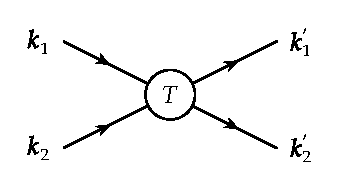
\includegraphics[width=0.45\linewidth]{pictures/4_1}
\par\end{centering}
\caption{\label{fig:T=0077E9=009635=007684=008D39=0066FC=0056FE=008868=00793A}$T$-矩阵的费曼图表示}
 
\end{figure}

可以证明，如果我们考虑两个核子在介质中的散射，定义一个类似于自由粒子散射矩阵的散射矩阵$G^{E}$是有意义的（这是在F.4节中导出的）。对于原子核中的核子，所要做的改变是比较显然的：平面波指标必须改为壳模型指标，方程\ref{eq:Lippmann-Schwinger equation}右侧分母上的单粒子动能必须用相应的壳模型能量来代替，并且中间态的求和范围必须被限制，使得它不包括费米面以下的态。最后一个改动是因为费米面以下的两个核子只能散射到费米面以上的态，因为所有其他能级都被占据
\begin{comment}
由此能量不守恒，所以肯定不行？
\end{comment}
。因此，我们得到下面关于$G$-矩阵的方程，它通常被称为Bethe-Goldstone方程\cite{BG57}（关于它的数学推导，见F.4节）。

\begin{equation}
G^{E}_{ab,cd}=\bar{v}_{ab,cd}+\frac{1}{2}\sum_{m,n>\varepsilon_{\text{F}}}\bar{v}_{ab,mn}\frac{1}{E-\varepsilon_{m}-\varepsilon_{n}+\mathrm{i}\eta}G^{E}_{mn,cd}\label{eq:Bethe-Goldstone equation}
\end{equation}

这里$ab,\dots,mn$是壳模型指标，$\varepsilon_{\text{F}}$是费米能。这个方程用图来表示会比较显然，正如\ref{fig:Bethe-Goldstone=0065B9=007A0B=007684=008D39=0066FC=0056FE=008868=00793A}中那样。连接两个相互作用的两条线代表“传播子''$1/(E-\varepsilon_{n}-\varepsilon_{m})$（在第八章和附录F中会有更详细的关于费曼图的解释）。对于$E<\varepsilon_{\text{F}}$的情况，我们可以忽略\ref{eq:Bethe-Goldstone equation}中分母上的$\mathrm{i}\eta$，在这种情况下$G$-矩阵显然是厄米的，这可以通过迭代利用\ref{eq:Bethe-Goldstone equation}看出。方程\ref{eq:Bethe-Goldstone equation}也可以写成算符形式：

\begin{figure}[H]
\begin{centering}
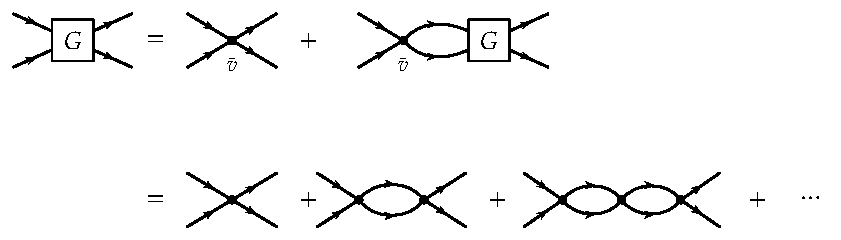
\includegraphics[width=0.7\linewidth]{pictures/4_2}
\par\end{centering}
\caption{\label{fig:Bethe-Goldstone=0065B9=007A0B=007684=008D39=0066FC=0056FE=008868=00793A}Bethe-Goldstone方程的费曼图表示}

\end{figure}

\begin{equation}
G=\bar{v}+\bar{v}\frac{Q_{F}}{E-H_{0}}G\label{eq:operator form Bethe-Goldstone equation}
\end{equation}

这里$H_{0}$是壳模型 Hamilton 量，$Q_{F}$是去掉了所有占据态的投影算符：
\begin{equation}
Q_{F}=\sum_{\begin{subarray}{c}
m<n\\
>\varepsilon_{\text{F}}
\end{subarray}}|mn\rangle\langle mn|\label{eq:project operator}
\end{equation}

我们可以从\ref{eq:operator form Bethe-Goldstone equation}定性地看出当$\bar{v}$无穷大的时候，$G$仍然是有限大的。形式地解\ref{eq:operator form Bethe-Goldstone equation}可以得到：

\[
G=\frac{\bar{v}}{1-\bar{v}Q_{F}/(E-H_{0})}
\]

如果$\bar{v}$是无穷大，$G$仍然是有限大的。这当然是一个粗糙的做法，接下来我们会用一个具体的例子更详细的说明这一点。在此之前，我们必须讨论方程\ref{eq:Bethe-Goldstone equation}的一些性质。尽管\ref{eq:Bethe-Goldstone equation}和\ref{eq:Lippmann-Schwinger equation}形式上很相近，但是还是有一些不同的地方需要注意的，例如类比自由粒子的散射波定义的$E<\varepsilon_{\text{F}}$的的波函数的边界条件{[}Me
61, 第XIX 10章{]}：
\begin{align}
|\psi_{ab}\rangle & \equiv\bar{v}^{-1}G|ab\rangle=\left(1+\frac{Q_{F}}{E-H_{0}}G\right)|ab\rangle\label{eq:G wave function}\\
 & =|ab\rangle+\frac{Q_{F}}{E-H_{0}}\bar{v}|\psi_{ab}\rangle\nonumber 
\end{align}

这里：
\[
\langle\boldsymbol{r}_{1}\boldsymbol{r}_{2}|ab\rangle=\frac{1}{\sqrt{2}}(\varphi_{a}(\boldsymbol{r}_{1})\varphi_{b}(\boldsymbol{r}_{2})-\varphi_{a}(\boldsymbol{r}_{2})\varphi_{b}(\boldsymbol{r}_{1}))
\]

另有：
\[
H_{0}|ab\rangle=(\varepsilon_{a}+\varepsilon_{b})|ab\rangle
\]

方程\ref{eq:G wave function}在形式上类似于散射波的方程。然而，在真正的散射中，式\ref{eq:G wave function}中的第二项给出了波函数的出射部分，因此当两个粒子的相对距离$\left|\boldsymbol{r}_{1}-\boldsymbol{r}_{2}\right|$趋于无穷大时并不为零，但在当前$E<\varepsilon_{F}$的情况下这一项是零。这是因为在真实的散射过程中，方程\ref{eq:Lippmann-Schwinger equation}中的$T$矩阵在得到方程\ref{eq:G wave function}时是“在壳的”，也就是说散射过程前后两个粒子的相对动量的绝对值必须相同，而且$E$必须对应于这个相对动量的值。因此，在真实的散射过程中\ref{eq:G wave function}中的分母可以是零，因此引入了一个奇点。然而这里并不是这样，由于我们假设了$E<\varepsilon_{\text{F}}$，因此方程\ref{eq:G wave function}右边的第二项绝对不可能是“在壳的”，所以它在$\left|\boldsymbol{r}_{1}-\boldsymbol{r}_{2}\right|$很大时变成了零。Day\cite{Da67}的一篇综述里有这些推导，然而，它太长而且也太偏离主题了，不适合在这里讨论。我们因此直接得到：
\[
|\psi^{E}_{ab}\rangle\xrightarrow{\left|\boldsymbol{r}_{1}-\boldsymbol{r}_{2}\right|\rightarrow\infty}|ab\rangle
\]

从方程\ref{eq:G wave function}和\ref{eq:project operator}可以立即得到$a,b<\varepsilon_{\text{F}}$时的归一化条件：
\[
\langle ij|\psi_{ij}\rangle=1\quad i,j<\varepsilon_{F}
\]

把关联对函数$|\psi_{ij}\rangle$用非关联的基展开也是对我们有启发的。从\ref{eq:G wave function}我们可以得到：
\[
|\psi_{ij}\rangle=|ij\rangle+\frac{1}{2}\sum_{mn}C^{ij}_{mn}|mn\rangle
\]

这意味着关联函数不仅包括$|ij\rangle$，也包括费米面以上的成分。可以证明在最重要的应用中$G$矩阵中的$E$都是在费米面以下的。例如，在Brückner-Hartree-Fock理论（第五章）中，我们必须在$i,j<\varepsilon_{\text{F}}$的情况下计算$G^{E=\varepsilon_{i}+\varepsilon_{j}}_{ab,ij}$。我们因此可以在这种情况下用一个简化但精确可解的模型来处理硬核芯，这一模型能展示最重要的特性。

让我们考虑一个非常大的核，它的内部应当和无限大的核也就是核物质非常相似。此外，我们做一个非常粗糙的假设，即相互作用只有一个硬核芯：
\[
\text{当}r\geq c\text{时}V(r)=0\quad\text{且}\quad\text{当}r<c\text{时}V(r)=\infty
\]

此外，我们假设有两个不可分辨粒子，例如一个质子和一个中子，这对于我们要阐释的原理来说以及足够了。现在我们把\ref{eq:G wave function}写成：
\[
(E-H_{0})|\psi_{ab}\rangle=(E-H_{0}+Q_{F}G)|ab\rangle
\]

在我们这种情况（$E=\varepsilon_{i}+\varepsilon_{j}$）下就是：
\begin{equation}
(\varepsilon_{i}+\varepsilon_{j}-H_{0})|\psi_{ij}\rangle=Q_{F}G|ij\rangle=Q_{F}\bar{v}|\psi_{ij}\rangle\label{eq:toy BG equation}
\end{equation}

这里后一个等号我们利用了\ref{eq:G wave function}。上述方程要比一般的Schrödinger方程更难解，因为$Q_{F}$是个非局域的积分算符。这可以在坐标表象下看出：
\[
\langle\boldsymbol{r}_{1}\boldsymbol{r}_{2}|Q_{F}|\boldsymbol{r}^{\prime}_{1}\boldsymbol{r}^{\prime}_{2}\rangle=\sum_{\begin{subarray}{c}
m<n\\
>\varepsilon_{\text{F}}
\end{subarray}}\langle\boldsymbol{r}_{1}\boldsymbol{r}_{2}|mn\rangle\langle mn|\boldsymbol{r}^{\prime}_{1}\boldsymbol{r}^{\prime}_{2}\rangle
\]

在核物质的情况下，方程\ref{eq:toy BG equation}中的单粒子波函数显然是平面波。为了简化，我们也假设单粒子能是纯动能（在介质环境中这并不是一般的情况）。由于平移不变性，核物质质心的移动是平凡的，由此我们得到：
\[
\langle\boldsymbol{r}_{1}\boldsymbol{r}_{2}|\psi_{ij}\rangle\rightarrow\psi_{\boldsymbol{p}_{1}\boldsymbol{p}_{2}}(\boldsymbol{r}_{1}\boldsymbol{r}_{2})=\frac{1}{(2\mathrm{\pi})^{3/2}}\mathrm{e}^{\mathrm{i}\boldsymbol{P}\cdot\boldsymbol{R}}\psi_{\boldsymbol{P}\boldsymbol{p}}(\boldsymbol{r})
\]

这里我们使用了质心系：
\begin{align}
\boldsymbol{P} & =\boldsymbol{p}_{1}+\boldsymbol{p}_{2} & \boldsymbol{p} & =\frac{1}{2}(\boldsymbol{p}_{1}-\boldsymbol{p}_{2})\nonumber \\
\boldsymbol{R} & =\frac{1}{2}(\boldsymbol{r}_{1}+\boldsymbol{r}_{2}) & \boldsymbol{r} & =\boldsymbol{r}_{1}-\boldsymbol{r}_{2}\label{eq:coordinate transformation}
\end{align}

利用所有这些假设，\ref{eq:toy BG equation}变成了：
\begin{align*}
 & \frac{\hbar^{2}}{2m}(p^{2}_{1}+p^{2}_{2}-\nabla^{2}_{1}+\nabla^{2}_{2})\psi_{\boldsymbol{p}_{1}\boldsymbol{p}_{2}}(\boldsymbol{r}_{1}\boldsymbol{r}_{2})\\
= & \frac{1}{(2\mathrm{\pi})^{6}}\int_{p^{\prime}_{1},p^{\prime}_{2}>k_{\text{F}}}\mathrm{d}^{3}\boldsymbol{p}^{\prime}_{1}\mathrm{d}^{3}\boldsymbol{p}^{\prime}_{2}\int\mathrm{d}^{3}\boldsymbol{r}^{\prime}_{1}\mathrm{d}^{3}\boldsymbol{r}^{\prime}_{2}\,\mathrm{e}^{\mathrm{i}(\boldsymbol{p}^{\prime}_{1}\cdot\boldsymbol{r}_{1}+\boldsymbol{p}^{\prime}_{2}\cdot\boldsymbol{r}_{2}-\boldsymbol{p}^{\prime}_{1}\cdot\boldsymbol{r}^{\prime}_{1}-\boldsymbol{p}^{\prime}_{2}\cdot\boldsymbol{r}^{\prime}_{2})}v(\left|\boldsymbol{r}^{\prime}_{1}-\boldsymbol{r}^{\prime}_{2}\right|)\psi_{\boldsymbol{p}_{1}\boldsymbol{p}_{2}}(\boldsymbol{r}^{\prime}_{1}\boldsymbol{r}^{\prime}_{2})
\end{align*}

根据\ref{eq:coordinate transformation}中质心系的变换，我们得到：
\[
\frac{\hbar^{2}}{m}(k^{2}+\nabla^{2}_{\boldsymbol{r}})\mathrm{e}^{\mathrm{i}\boldsymbol{P}\cdot\boldsymbol{R}}\psi_{\boldsymbol{P}\boldsymbol{k}}(\boldsymbol{r})=\frac{1}{(2\mathrm{\pi})^{6}}\int_{\left|\frac{\boldsymbol{P}^{\prime}}{2}\pm\boldsymbol{p}^{\prime}\right|>k_{\text{F}}}\mathrm{d}^{3}\boldsymbol{P}^{\prime}\mathrm{d}^{3}\boldsymbol{p}^{\prime}\mathrm{d}^{3}\boldsymbol{R}^{\prime}\mathrm{d}^{3}\boldsymbol{r}^{\prime}\,\mathrm{e}^{\mathrm{i}[\boldsymbol{P}^{\prime}\cdot(\boldsymbol{R}-\boldsymbol{R}^{\prime})+\boldsymbol{p}^{\prime}\cdot(\boldsymbol{r}-\boldsymbol{r}^{\prime})]}v(r^{\prime})\mathrm{e}^{\mathrm{i}\boldsymbol{P}\cdot\boldsymbol{R}^{\prime}}\psi_{\boldsymbol{P}\boldsymbol{p}}(\boldsymbol{r}^{\prime})
\]

由于$\mathcal{P}^{2}=p^{2}+2pp^{\prime}\cos\theta+p^{\prime2}$，我们看到，即使在限制$p,p^{\prime}>k_{\text{F}}$下，$\mathcal{P}$也可以取从$0$到$\infty$的所有值。对$\boldsymbol{R}^{\prime}$的积分给出$\delta(\boldsymbol{P}-\boldsymbol{\mathcal{P}})$，因此我们也可以执行$\boldsymbol{\mathcal{P}}$积分。由此我们得到以下方程：
\begin{equation}
\frac{\hbar^{2}}{m}\{k^{2}+\Delta_{\boldsymbol{r}}\}\psi_{\boldsymbol{P}\boldsymbol{k}}(\boldsymbol{r})=\frac{1}{(2\mathrm{\pi})^{3}}\int_{\left|\frac{1}{2}\boldsymbol{P}\pm\boldsymbol{p}\right|>k_{\text{F}}}\mathrm{d}^{3}\boldsymbol{p}\,\mathrm{e}^{\mathrm{i}\boldsymbol{p}\cdot\boldsymbol{r}}\int\mathrm{d}^{3}\boldsymbol{r}^{\prime}\,\mathrm{e}^{-\mathrm{i}\boldsymbol{p}\cdot\boldsymbol{r}^{\prime}}v(\boldsymbol{r}^{\prime})\psi_{\boldsymbol{P}\boldsymbol{k}}(\boldsymbol{r}^{\prime})\label{eq:4.56}
\end{equation}

这个方程不仅因为其积分微分结构而比通常的双粒子方程更为复杂，而且还因为波函数对质心动量$\boldsymbol{P}$具有非平凡的依赖性。对于我们的目的而言，将其在$\boldsymbol{P}=0$处求值就足够了。此外，我们可以将\ref{eq:4.56}进行分波展开
\cite[第 X 章第 8 节]{Me61}：
\begin{equation}
\psi_{\boldsymbol{k}}(\boldsymbol{r})=\sum_{lm}\psi_{kl}(r)Y_{lm}(\theta,\varphi)\label{eq:4.57}
\end{equation}

考虑$s$波方程并将\ref{eq:4.56}中的积分拆分为两部分，即$\int^{\infty}_{k_{\text{F}}}=\int^{\infty}_{0}-\int^{k_{\text{F}}}_{0}$，我们得到：
\begin{equation}
\frac{\hbar^{2}}{m}\left(k^{2}+\frac{\partial^{2}}{\partial r^{2}}+\frac{2}{r}\frac{\partial}{\partial r}\right)\psi_{k}(r)=v(r)\psi_{k}(r)-(4\mathrm{\pi})^{2}\int^{k_{\text{F}}}_{0}\frac{\mathrm{d}p\,p^{2}}{(2\mathrm{\pi})^{3}}j_{0}(pr)\int^{\infty}_{0}\mathrm{d}r^{\prime}\,r^{\prime2}j_{0}(pr^{\prime})v(r^{\prime})\psi_{k}(r^{\prime})\label{eq:4.58}
\end{equation}
其中$j_{0}$是最低阶球 Bessel 函数。令$\psi_{k}(r)=(1/r)u_{k}(r)$，我们最终得到：
\begin{equation}
\frac{\hbar^{2}}{m}\left(k^{2}+\frac{\partial^{2}}{\partial r^{2}}\right)u_{k}(r)=v(r)u_{k}(r)-k_{\text{F}}\int^{\infty}_{0}\mathrm{d}r^{\prime}\,\chi(r,r^{\prime})v(r^{\prime})u_{k}(r^{\prime})\label{eq:4.59}
\end{equation}
其中
\begin{equation}
\chi(r,r^{\prime})=\frac{2rr^{\prime}}{\mathrm{\pi}k_{\text{F}}}\int^{k_{\text{F}}}_{0}\mathrm{d}p\,p^{2}j_{0}(pr)j_{0}(pr^{\prime})=\frac{1}{\mathrm{\pi}k_{\text{F}}}\left\{ \frac{\sin k_{\text{F}}(r-r^{\prime})}{r-r^{\prime}}-\frac{\sin k_{\text{F}}(r+r^{\prime})}{r+r^{\prime}}\right\} \label{eq:4.60}
\end{equation}

现在引入以下无量纲量是十分便利的：
\begin{equation}
x=k_{\text{F}}r;\quad x^{\prime}=k_{\text{F}}r^{\prime};\quad K=\frac{k}{k_{\text{F}}};\quad\frac{mv}{k^{2}_{\text{F}}\hbar^{2}}=w\label{eq:4.61}
\end{equation}
这导致
\begin{equation}
\left(\frac{\mathrm{d}^{2}}{\mathrm{d}x^{2}}+K^{2}\right)u_{K}(x)=w(x)u_{K}(x)-\int^{\infty}_{0}\mathrm{d}x^{\prime}\,\chi(x,x^{\prime})w(x^{\prime})u_{K}(x^{\prime})\label{eq:4.62}
\end{equation}

对于有限高度的方势垒，波函数及其一阶导数在势垒边缘处是连续的。我们很容易确信，当势垒高度趋于无穷大时，波函数的一阶导数在边缘处变得不连续，即：
\begin{equation}
u^{\prime}_{K}(c+\epsilon)=A\label{eq:4.63}
\end{equation}
其中$A$是一个常数，$r=c$是硬芯半径，而$\epsilon$是一个无穷小的正量。为了使\ref{eq:4.62}中的$u$产生这种不连续性，乘积$w\cdot u$在$r=c$处必须正比于$\delta$函数。由于对于$r>c$势$w$为零且$u$有限，乘积$w\cdot u$在硬芯半径外部消失。波函数$u$无法穿透到无限硬芯内部（$u\equiv0$）；因为在那里$w=\infty$，乘积$w\cdot u$可以是有限的，记$c^{\prime}=ck_{\text{F}}$，我们可以写出：
\begin{equation}
w(x)u_{K}(x)=A\delta(x-c^{\prime})+l(x)\theta(c^{\prime}-x)\label{eq:4.64}
\end{equation}
函数$l(x)$可以通过要求对于$x<c^{\prime}$，\ref{eq:4.62}的左侧必须为零来确定，因为对于$x<c^{\prime}$有$u\equiv0$。因此由\ref{eq:4.62}结合\ref{eq:4.64}，我们有：
\begin{equation}
l(x)=A\chi(x,c^{\prime})+\int^{c^{\prime}}_{0}\mathrm{d}x^{\prime}\,\chi(x,x^{\prime})l(x^{\prime})\quad(x<c^{\prime})\label{eq:4.65}
\end{equation}
由于硬芯通常相当小（对于$c=0.4\,\text{fm}$在核物质密度下$c^{\prime}=0.57$），我们可以展开\ref{eq:4.65}中的积分核，并从\ref{eq:4.60}得到：
\begin{equation}
\chi(x,x^{\prime})\rightarrow\frac{2xx^{\prime}}{3\mathrm{\pi}}\quad(x<c^{\prime},\;x^{\prime}<c^{\prime})\label{eq:4.66}
\end{equation}
结合\ref{eq:4.66}和\ref{eq:4.65}，我们看到$l(x)$是$c^{\prime2}$量级的，而对$l(x)$的任何积分都将是$c^{\prime3}$量级的。因此在\ref{eq:4.62}中我们可以忽略\ref{eq:4.64}中的第二项，从而得到在$c^{\prime}$的一阶近似下准确的结果：
\begin{align}
\left(\frac{\mathrm{d}^{2}}{\mathrm{d}x^{2}}+K^{2}\right)u_{K}(x) & \simeq A[\delta(x-c^{\prime})-\chi(x,c^{\prime})]+A\chi(x,c^{\prime})\theta(c^{\prime}-x)\nonumber \\
 & =A\frac{2xc^{\prime}}{\mathrm{\pi}}\int^{\infty}_{1}\mathrm{d}p\,p^{2}j_{0}(px)j_{0}(pc^{\prime})+A\chi(x,c^{\prime})\theta(c^{\prime}-x)\nonumber \\
 & =F(x)\label{eq:4.67}
\end{align}
其中我们利用了恒等式：
\begin{equation}
\int^{\infty}_{0}\mathrm{d}p\,p^{2}j_{l}(pr)j_{l}(pr^{\prime})=\frac{\mathrm{\pi}}{2r^{2}}\delta(r-r^{\prime})\label{eq:4.68}
\end{equation}

我们指出，由于\ref{eq:4.67}的右侧仅在$c^{\prime}$的一阶下是精确的，是否保留\ref{eq:4.67}右侧属于二阶项的第二项在某种程度上是任意的。方程\ref{eq:4.67}的通解：
\begin{equation}
u_{K}(x)=\frac{\sin Kx}{K}\int^{x}_{c^{\prime}}\mathrm{d}y\,F(y)\cos Ky-\frac{\cos Kx}{K}\int^{x}_{c^{\prime}}\mathrm{d}y\,F(y)\sin Ky\label{eq:4.69}
\end{equation}
在$x=c^{\prime}$处显然为零。直接代入即可容易地验证方程\ref{eq:4.69}确实是方程\ref{eq:4.67}的解。

解\ref{eq:4.67}与\ref{eq:4.69}中唯一的未知量是常数$A$，我们将通过要求$u_{K}$渐近趋近于未微扰值这一条件\ref{eq:toy BG equation}来确定它。为此，我们首先证明在$x\rightarrow\infty$极限下，\ref{eq:4.69}右侧的第二个积分为零。由于我们在极小$c^{\prime}$的极限下考虑解，我们可以将积分限从$c^{\prime}$到$\infty$取为从$0$到$\infty$，从而有：
\begin{align}
\frac{1}{K}\int^{\infty}_{0}\mathrm{d}y\,F(y)\sin Ky & =\frac{2Ac^{\prime}}{\mathrm{\pi}}\int^{\infty}_{1}\mathrm{d}p\,p^{2}j_{0}(pc^{\prime})\int^{\infty}_{0}\mathrm{d}y\,y^{2}j_{0}(Ky)j_{0}(py)\nonumber \\
 & =\frac{2Ac^{\prime}}{\mathrm{\pi}}\int^{\infty}_{1}\mathrm{d}p\,p^{2}j_{0}(pc^{\prime})\frac{\mathrm{\pi}}{2Kp}\delta(K-p)\nonumber \\
 & =0\label{eq:4.70}
\end{align}
最后的积分之所以消失，是因为$p$在 Fermi 球之外，而$K$在 Fermi 球之内。因此对于$r\rightarrow\infty$，我们发现波函数趋近于未微扰结果（$\psi\rightarrow j_{0}$）当且仅当：
\begin{equation}
\int^{\infty}_{0}\mathrm{d}y\,F(y)\cos Ky=1\label{eq:4.71}
\end{equation}
于是利用\ref{eq:4.67}，我们得到：
\begin{equation}
A=\left\{ \cos Kc^{\prime}-\int^{\infty}_{0}\mathrm{d}y\,\cos(Ky)\chi(y,c^{\prime})\right\} ^{-1}\label{eq:4.72}
\end{equation}
这完成了对硬球势的波函数$u_{K}(x)$的确定。

\begin{figure}[H]
\begin{centering}
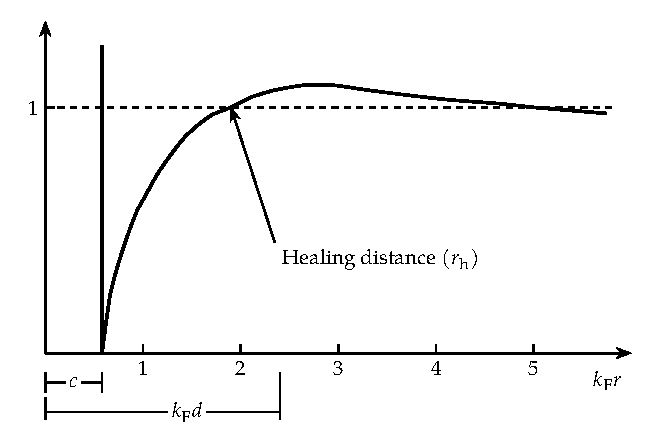
\includegraphics[width=0.65\linewidth]{pictures/4_3}
\par\end{centering}
\caption{\label{fig:4_3}核物质中纯硬芯势的 Bethe–Goldstone 方程的 S 波解。有关图形细节见正文（引自 \cite{FW71}）}
\end{figure}

在图 \ref{fig:4_3} 中，我们展示了对应于$k=0$的解$\psi_{k}(r)$，它揭示了若干有趣的特征。波函数在硬芯内部严格为零。由\ref{eq:4.69}和\ref{eq:4.72}容易看出，它迅速（通过阻尼振荡）趋近于无相互作用核子对的波函数值（对于$k=0$且在所有$r$处该值恒等于
1）。波函数首次达到未微扰值时的$r$值称为\textbf{复原距离}（healing distance）$r_{h}$，因为只有在小于该距离处，硬芯波函数才与未微扰波函数有显著差异。对于我们例子中所选取的数值，复原距离为：
\begin{equation}
k_{\text{F}}r_{h}\simeq1.9\label{eq:4.73}
\end{equation}
（对\ref{eq:4.59}更普遍的研究表明，该值或多或少与$\boldsymbol{P}$和$k$无关 \cite{WG67a}）。值得特别注意的是，这一数值明显小于核物质中的平均粒子间距$d$，后者由表达式$1/d^{3}\equiv N/V=(4\int_{p\le\hbar k_{\text{F}}}\mathrm{d}p\int\mathrm{d}r)/V(2\mathrm{\pi}\hbar)^{3}=2k^{3}_{\text{F}}/(3\mathrm{\pi}^{2})$定义，给出粒子间距为：
\begin{equation}
k_{\text{F}}d=\left(\frac{3\mathrm{\pi}^{2}}{2}\right)^{1/3}=2.46\label{eq:4.74}
\end{equation}

因此平均而言，核子在碰撞之后、下一次碰撞发生之前，就已经恢复为其独立粒子波函数。因此，核波函数的绝大部分由独立粒子波函数构成的行列式组成。这可以视为独立粒子模型合理性的论证——Pauli
原理抑制了散射过程的低动量成分，也就是说，抑制了长程关联。正是由于不相容原理，核子在核内的大多数时间里都表现为独立粒子而运动。Weisskopf
首先指出强相互作用但稀薄的 Fermi 气体中可能发生这种现象 \cite{We50}。

我们已经看到，求解 Bethe–Goldstone 方程\ref{eq:toy BG equation}绝非平凡之事；人们很容易想象，对于波函数不再是平面波且失去平移不变性的有限核，这项任务将变得极其困难。因此目前人们采用了若干近似方案。正如我们在例子中所看到的，正是投影算符$Q_{\text{F}}$使得求解变得十分困难。Moszkowski
与 Scott 的\textbf{分离方法}（separation method）\cite{MS60} 以及 Bethe、Brandow
和 Petschek 的\textbf{参考谱方法}（reference spectrum method）\cite{BBP63}
提出，Pauli 原理应当仅作为微扰来处理。我们不打算深入探讨这些近似方法的细节，读者可参阅 Brown \cite{Br64}、de
Shalit 与 Feshbach \cite{SF74} 的专著以及 Bethe 的综述文章 \cite{Be71}，其中详细阐述了这些方法以及利用谐振子基求解有限核
Bethe–Goldstone 方程等进一步方案。在此我们仅提一下最近在 Brueckner–Hartree–Fock 理论中取得极大成功的另一近似方案（见第
5 章）。这就是 Negele 的\textbf{局域密度近似}（local density approximation, LDA）\cite{Ne70,Ne75}，它最初由
Brueckner、Gammel 和 Weitzner \cite{BGW58} 以及 Brueckner、Lockett 和 Rotenberg
\cite{BLR61} 引入。其基本假设是：有限核中任何局域位置处的$G$矩阵与处于相同密度的无限核物质的$G$矩阵相同，从而在局域上可以像在核物质计算中一样计算$G$矩阵
\cite{Be71,Ne75}。我们将在第 5 章重返这一近似。

\subsection{价核子之间的有效相互作用}

Brueckner $G$矩阵具有重要应用的另一个领域是所谓的\textbf{价核子}之间的有效核力（评述参见 \cite{Ku74b}
及其文献）。作为一个确切的例子，我们考察$^{18}\mathrm{O}$或$^{18}\mathrm{F}$，它们是在双幻核$^{16}\mathrm{O}$芯之上具有两个核子（“价核子”）。在纯壳模型近似中，这两个核子将处于$1d_{5/2}$能级上。我们有望通过使用刚好构成$^{16}\mathrm{O}$芯之上的第一个壳层的$1d_{5/2},2s_{1/2},1d_{3/2}$单粒子态进行组态混合计算，来很好地描述$^{18}\mathrm{O}$的低激发态。此类壳模型计算在第
2 章中已作了一定程度的阐述，并在第 8 章中更详细地处理；例如在第 8 章中我们将证明，这类双价核子体系可以很好地由粒子-粒子 Tamm–Dancoff
久期方程来描述 {[}参见第 8 章式 (8.10){]}：
\begin{equation}
(E^{\text{TD}}_{\rho}-\epsilon_{m}-\epsilon_{n})R^{\rho}_{mn}=\frac{1}{2}\sum_{m^{\prime}n^{\prime}}\bar{v}_{mn,m^{\prime}n^{\prime}}R^{\rho}_{m^{\prime}n^{\prime}}\label{eq:4.75}
\end{equation}
这里的$\epsilon_{m}$是唯象或自洽（见第 5 章）单粒子 Hamilton 量$H_{0}$的单粒子能量，且\ref{eq:4.75}中的所有指标都处于芯的
Fermi 能级以上的\textbf{模型空间}中（在我们的例子中即为$d_{5/2},2s_{1/2},d_{3/2}$态）。对于\ref{eq:4.75}中的双粒子相互作用，我们不能直接采用裸相互作用，因为该力必须模拟并至少近似修正：（a）Fermi
能级以上双粒子组态其余部分的忽略；（b）来自壳模型基更高组态（如$3p-1h,4p-2h$等）的贡献。

下面我们将推导一个精确方程，形式上与\ref{eq:4.75}几乎完全相同，但其中的$\bar{v}$被替换为一个原则上可以从裸相互作用（例如
Hamada–Johnston 势）计算出来的有效（依赖于能量的）相互作用。我们从第 2 章关于壳模型提供一组完全态的结论出发；因此任何精确波函数都可以在该基矢下展开。进行这种展开的一个便捷方法是二次量子化形式，例如$A+2$核子体系态的展开可以写为以下形式（亦见第
8 章；在下文中，指标$m,n,r,p$与$i,j$分别表示处于 Fermi 能级以上和以下的态）：
\begin{align}
|A+2,\tau\rangle & =\sum_{m<n}R^{\tau}_{mn}a^{\dagger}_{m}a^{\dagger}_{n}|\text{HF}\rangle+\sum_{m<n<r,i}R^{\tau}_{mnr,i}a^{\dagger}_{m}a^{\dagger}_{n}a^{\dagger}_{r}a_{i}|\text{HF}\rangle\nonumber \\
 & \quad+\sum_{\begin{subarray}{c}
m<n<r<p\\
i<j
\end{subarray}}R^{\tau}_{mnrp,ij}a^{\dagger}_{m}a^{\dagger}_{n}a^{\dagger}_{r}a^{\dagger}_{p}a_{i}a_{j}|\text{HF}\rangle+\cdots\label{eq:4.76}
\end{align}
此展开中的第一项对应于\ref{eq:4.75}模型空间中保留的态。其它各项则分别代表$3p-1h,4p-2h$等组态。

在第 2 章中我们看到，全部 Slater 行列式的集合同样提供了一组完备态。设精确 Hamilton 量为$H=T+V$，其中$T$为动能，$V$为裸双体相互作用。我们希望对$A+2$粒子体系求解精确
Schrödinger 方程：
\begin{equation}
H|\Psi_{\tau}\rangle=E_{\tau}|\Psi_{\tau}\rangle\label{eq:4.77}
\end{equation}
类似于 Bethe–Goldstone 方程\ref{eq:operator form Bethe-Goldstone equation}，我们将再次利用投影算符来消除未包含在模型空间中的组态。为此我们定义向模型空间（在我们情形中即$2p-0h$态）投影的投影算符$P$：
\begin{equation}
P=\sum_{m<n}a^{\dagger}_{m}a^{\dagger}_{n}|\text{HF}\rangle\langle\text{HF}|a_{n}a_{m}\label{eq:4.78}
\end{equation}
其中指标$m,n$遍历模型空间中包含的所有单粒子态。向 Hilbert 空间的其余部分投影的算符$Q$定义为：
\begin{equation}
Q=1-P\label{eq:4.79}
\end{equation}
利用$P+Q=1$，我们可以将 Schrödinger 方程\ref{eq:4.77}改写为一组耦合方程：
\begin{align}
(E_{\tau}-PHP)P|\Psi_{\tau}\rangle & =PHQ\,Q|\Psi_{\tau}\rangle\label{eq:4.80}\\
(E_{\tau}-QHQ)Q|\Psi_{\tau}\rangle & =QHP\,P|\Psi_{\tau}\rangle\label{eq:4.81}
\end{align}
这就是著名的 Feshbach 投影算符形式 \cite{Fe62}。由于按照假设我们只想计算波函数在模型空间上的投影$P|\Psi_{\tau}\rangle$，我们可以从\ref{eq:4.81}中形式解出$Q|\Psi_{\tau}\rangle$：
\begin{equation}
Q|\Psi_{\tau}\rangle=\frac{1}{E_{\tau}-QHQ}QHP\,P|\Psi_{\tau}\rangle\label{eq:4.82}
\end{equation}
并将此代入\ref{eq:4.80}，从而得到一个完全在模型空间中作用的方程：
\begin{equation}
(PHP+V_{\text{eff}}(E_{\tau}))P|\Psi_{\tau}\rangle=E_{\tau}P|\Psi_{\tau}\rangle\label{eq:4.83}
\end{equation}
其中
\begin{equation}
V_{\text{eff}}(E)=PHQ\frac{1}{E-QHQ}QHP\label{eq:4.84}
\end{equation}

我们看到在方程\ref{eq:4.83}中本征值仍是精确本征值$E_{\tau}$，而波函数只是精确波函数在模型空间上的投影。通过与态$a^{\dagger}_{m}a^{\dagger}_{n}|\text{HF}\rangle$取矩阵元，方程\ref{eq:4.83}可以化为\ref{eq:4.75}的形式。将
Hamilton 量$H$写为$H=H_{0}+V-U$，其中$H_{0}=T+U$为壳模型 Hamilton 量，我们得到：
\begin{equation}
(E_{\tau}-E^{\text{HF}}_{0}-\epsilon_{m}-\epsilon_{n})R^{\tau}_{mn}=\frac{1}{2}\sum_{m^{\prime}n^{\prime}}\langle mn|V_{\text{eff}}(E_{\tau})|m^{\prime}n^{\prime}\rangle R^{\tau}_{m^{\prime}n^{\prime}}\label{eq:4.85}
\end{equation}
其中
\begin{equation}
R^{\tau}_{mn}=\langle\text{HF}|a_{n}a_{m}|\Psi_{\tau}\rangle\label{eq:4.86}
\end{equation}
以及
\begin{equation}
V_{\text{eff}}(E)=P(V-U)P+P(V-U)Q\frac{1}{E-QHQ}Q(V-U)P\label{eq:4.87}
\end{equation}
这里$E^{\text{HF}}_{0}$为芯的 Hartree–Fock 能量，单粒子态选为$H_{0}$的本征态。在推导\ref{eq:4.85}时，我们忽略了$U$的粒子-粒子矩阵元，这在具有较大芯核的情形下是很小的\footnote{$V_{\text{eff}}$的非厄米性质可以通过一种略微不同的定义来避免 {[}参见 Brandow \cite{Br67a}
和 Kuo 等人 \cite{KLR71}{]}。这一引入所谓折叠图（folded diagrams）的形式体系也是不依赖于能量的，但包含了在$G$的高阶项。}。

方程\ref{eq:4.85}具有非线性本征值问题的形式，因为有效相互作用$V_{\text{eff}}$本身依赖于本征值$E_{\tau}$。在实际计算中，通常用平均值$\bar{E}$替代$E_{\tau}$，并将\ref{eq:4.85}作为普通的线性本征值问题求解。投影算符$Q$可以分解为投影到模型空间之外的$2p-0h$态的部分$Q_{2p}$，投影到$3p-1h$态的部分$Q_{3p-1h}$，等等：$Q=Q_{2p}+Q_{3p-1h}+Q_{4p-2h}+\cdots$。如果在\ref{eq:4.87}的投影算符$Q$中只保留$Q_{2p}$并忽略分母中的$U$，则有效相互作用等于将$\epsilon_{\text{F}}$替换为$\epsilon_{\max}$的
Brueckner $G$矩阵\ref{eq:toy BG equation}，即：
\begin{equation}
(V^{(2p)}_{\text{eff}})_{mn,m^{\prime}n^{\prime}}=G^{E^{A+2}_{0}-E^{A}_{0}}_{mn,m^{\prime}n^{\prime}}(\epsilon_{\text{F}}\rightarrow\epsilon_{\max})\label{eq:4.88}
\end{equation}

将精确 Schrödinger 方程改写为\ref{eq:4.85}形式的全部初衷与哲学，均建立在这样一种期望之上：即对于双价核子的物理问题，算符$V_{\text{eff}}$可以通过某种微扰方法在很好近似下计算出来。因此必须假设$V_{\text{eff}}$是良态的，例如它没有强烈的能量依赖性。因此通常忽略\ref{eq:4.88}中$G$的能量依赖，并用下式替代：
\begin{equation}
\Omega_{\tau}\simeq\frac{1}{2}(\epsilon_{m}+\epsilon_{n}+\epsilon_{m^{\prime}}+\epsilon_{n^{\prime}})\label{eq:4.89}
\end{equation}
此外，通常用于求解 Bethe–Goldstone 方程的所有其它近似也不应对结果产生过大影响（参见 \cite{Ma69} 与
\cite{SF74}）。Kuo 与 Brown \cite{KB66} 在谐振子近似下求解了$^{18}\mathrm{O}$和$^{18}\mathrm{F}$的
Bethe–Goldstone 方程，其中裸相互作用采用 Hamada–Johnston 力。随后在\ref{eq:4.85}中利用该力在模型空间中进行对角化，其中单粒子能量取自$^{17}\mathrm{O}$的实验测定值。在图
\ref{fig:4_4} 中，我们给出了这些作者计算的$^{18}\mathrm{O}$低能谱与实验谱的比较；在图 \ref{fig:4_5}
中，我们对$^{210}\mathrm{Pb}$情形展示了同样的结果。后者的计算由 Herling 与 Kuo \cite{HK72}
原则上采用与 Kuo–Brown 相同的方法完成，其模型空间由以下单粒子态构成：

中子：$2g_{9/2},1i_{11/2},1j_{15/2},3d_{5/2},4s_{1/2},2g_{7/2},3d_{3/2}$

质子：$1h_{9/2},2f_{7/2},1i_{13/2},2f_{5/2},3p_{3/2},3p_{1/2}$

\begin{figure}[H]
\begin{centering}
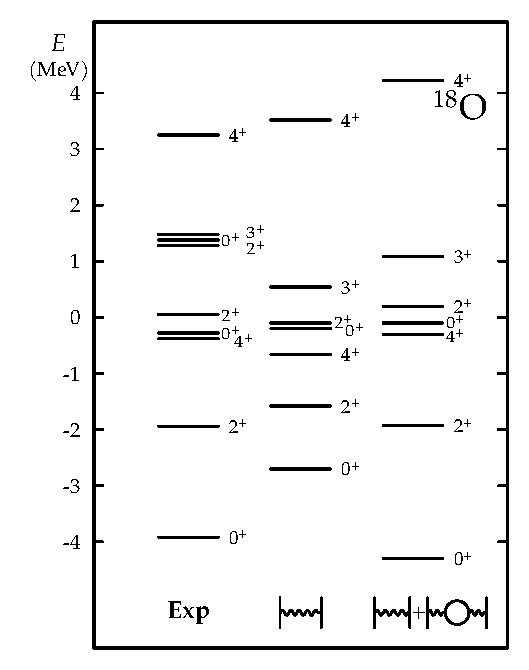
\includegraphics[width=0.5\linewidth]{pictures/4_4}
\par\end{centering}
\caption{\label{fig:4_4}$^{18}\mathrm{O}$的能谱。第一列为实验值；第二列采用纯 $G$ 矩阵计算；第三列同时包含了极化项
(4.90)（引自 \cite{HK72}）}
\end{figure}

\begin{figure}[H]
\begin{centering}
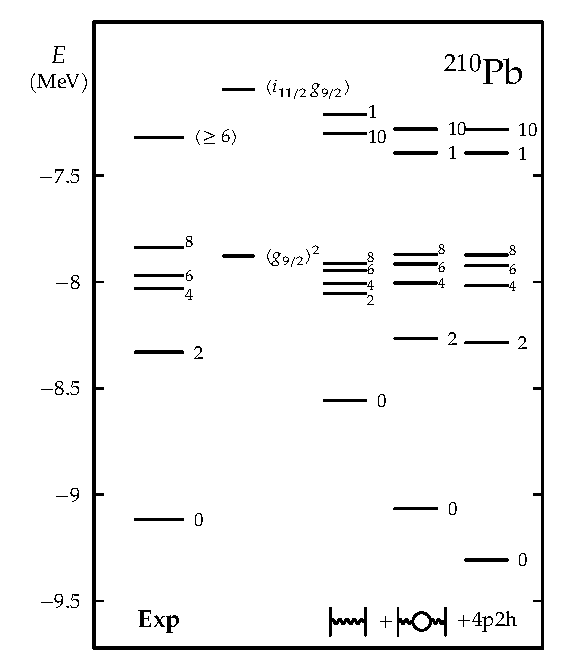
\includegraphics[width=0.55\linewidth]{pictures/4_5}
\par\end{centering}
\caption{\label{fig:4_5}$^{210}\mathrm{Pb}$的能谱。前三列谱的含义与图 \ref{fig:4_4} 相同；在第四列谱中亦考虑了
$4p-2h$ 极化项。图中同时标出了自由双粒子能量（引自 \cite{HK72}）}
\end{figure}

正如从图 \ref{fig:4_4} 和图 \ref{fig:4_5} 中所见，这两项计算与实验的比较并不十分令人满意，其吻合只能被认为是定性的。这种分歧大概并非源于求解
Bethe–Goldstone 方程所引入的各种近似，而是由于忽略了$3p-1h$等其它组态。在上述两项计算中均已表明，至少在微扰论中包含$3p-1h$组态可以极大地改善与实验的一致性。具体步骤是在二阶微扰论中计算\ref{eq:4.83}和\ref{eq:4.85}中来自$Q_{3p-1h}$对$V_{\text{eff}}$的贡献（略去非连通项，见关于折叠图的脚注）。利用我们的定义式，这并不难执行，其结果为：
\begin{equation}
(V^{3p-1h}_{\text{eff}})_{mn,m^{\prime}n^{\prime}}=\left\{ \sum_{pi}\frac{\bar{v}_{mi,m^{\prime}p}\bar{v}_{pn,in^{\prime}}}{\Omega_{\tau}-\epsilon_{m^{\prime}}-\epsilon_{n}-\epsilon_{p}+\epsilon_{i}}-(n^{\prime}\leftrightarrow m^{\prime})\right\} -(m\leftrightarrow n)\label{eq:4.90}
\end{equation}

\begin{figure}[H]
\begin{centering}
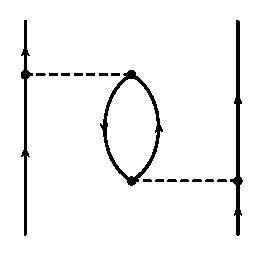
\includegraphics[width=0.28\linewidth]{pictures/4_6}
\par\end{centering}
\caption{\label{fig:4_6}芯极化项的图解表示}
\end{figure}

在这一表达式中，我们忽略了所有使单粒子能量重正化的项，即具有结构$(V_{\text{eff}})_{mn,m^{\prime}n^{\prime}}=A_{mm^{\prime}}B_{nn^{\prime}}-(m^{\prime}\leftrightarrow n^{\prime})$的项，因为通常认为这些项已经包含在具体计算所采用的实验单粒子能中了。通常人们将项\ref{eq:4.90}用图形表示，如图
\ref{fig:4_6} 所示（关于 Feynman 图的更多内容在第 8 章和附录 F 中解释）。然而由于硬芯势的存在，二阶部分不能直接按原样使用。文献
\cite{BK67a} 表明，在$3p-1h$态对$V_{\text{eff}}$的二阶贡献中将裸相互作用替换为其相应的$G$矩阵，正是高阶项的一种自洽重求和。我们在此不详述这些论证，因为它们超出了本书的范围。在图
\ref{fig:4_4} 和图 \ref{fig:4_5} 中也展示了包含这些“重正化”二阶$3p-1h$贡献（即“\textbf{芯极化}”）的结果；可以看出，在两种情形下计算与实验的吻合都近乎完美。如果这就是全部事实，那么结果将是非常令人满意的，因为我们基本上无需引入任何自由参数就解释了这些原子核能谱的低激发部分。

遗憾的是，问题远未彻底解决，因为后续研究表明，包含更高阶项反而会再次使结果恶化。这一效应在图 \ref{fig:4_5} 中清晰体现，其中不仅包含了$3p-1h$项，还包含了$4p-2h$项。Barrett
与 Kirson \cite{BK73} 以及 Kirson 与 Zamick \cite{KZ70} 在这方面进行了更系统但更复杂的深入研究，结果表明不同高阶项的作用导致能谱剧烈涨落，因而无法得出明确结论；特别是，为何二阶$3p-1h$项的引入能与实验达成如此优异的一致性，至今仍未得到彻底阐明。因此人们不得不得出结论：有效相互作用的微观理论仍处于远非令人满意的阶段。

尽管如此，我们仍想回到理论中的两个形式要点。第一点关乎有效相互作用$V^{E}_{\text{eff}}$的能量依赖性。在上述所有计算中，这种能量依赖性或多或少都被忽略了。正如我们已指出的，只要能量依赖性确实很微弱，这种处理当然是成立的。然而实际中$V^{E}_{\text{eff}}$作为$E$的函数可能存在极点，且这些极点可能紧邻甚至落入所关心的低激发态能量区域；例如对于$^{18}\mathrm{O}$即是如此，其中一个集体性的$4p-2h$极点能量降得非常低
\cite{Sch75}。在这种情形下，该极点必须单独处理，因为它在所关心的能量区间内引起了强烈的能量依赖性。这些态在折叠图形式体系中也带来了困难，并被称为\textbf{侵入态}（intruder
states）\cite{SW72,SW73}。在这些情形中，相应有效相互作用按$G$矩阵幂次的微扰展开式极有可能是发散的。人们已经发展了处理这一问题的专门技术
\cite{SW72,SW73,HLR74}。迄今为止我们仅考虑了双核子体系，然而对于多于两个价核子的情形亦可作同样的考量 \cite{Ma69}，尽管我们不打算深入这些细节。

\subsection{粒子-空穴间的有效相互作用}

粒子与空穴间有效相互作用的问题主要出现在闭壳核振动态的研究中（见第 8 章）。然而从微观视角来看，该情形受到的研究远少于价核子之间的相互作用（参见例如
\cite{BK69,KBB70}）。人们可以认为，若能将有效的$ph$力同样用微观$G$矩阵辅以某些高阶修正（如价核子中的极化图）来表示，将是非常理想的。事实上，这一目标确实能够实现。由于在很大程度上，对于$ph$体系被公认为恰当理论的是随机相位近似（RPA，见第
8 章）而非 Tamm–Dancoff 近似（TDA），这使得讨论更为复杂。然而为了不使问题过于繁冗，我们将仅局限于 Tamm–Dancoff
近似情形。

Tamm–Dancoff 方程（见第 8 章）具有以下形式：
\begin{equation}
(E^{\text{TDA}}_{\mu}-\epsilon_{m}+\epsilon_{i})C^{\mu}_{mi}=\sum_{nj}\bar{v}_{mj,in}C^{\mu}_{nj}\label{eq:4.91}
\end{equation}
其中$m,n$（$i,j$）为 Fermi 面以上（以下）的指标。该方程通常在一个模型空间中求解，例如取 Fermi 面之上一壳和之下一壳。类似于双价核子的情形，进入式\ref{eq:4.91}的唯象相互作用必须模拟未包含在模型空间中的$1p-1h$态以及$2p-2h,3p-3h$等态的效应。

一般而言，对于闭壳核我们可以将这种振动态作如下展开（见第 8 章）：
\begin{equation}
|\mu\rangle=\sum_{mi}C^{\mu}_{mi}a^{\dagger}_{m}a_{i}|\text{HF}\rangle+\sum_{\begin{subarray}{c}
m<n\\
i<j
\end{subarray}}C^{\mu}_{mn,ij}a^{\dagger}_{m}a^{\dagger}_{n}a_{i}a_{j}|\text{HF}\rangle+\cdots\label{eq:4.92}
\end{equation}
然而，从式\ref{eq:4.92}出发获得有效相互作用的步骤与价核子情形略有不同。首先我们引入向\textbf{整个}$1p-1h$子空间投影的投影算符$P$：
\begin{align}
P & =\sum_{mi}a^{\dagger}_{m}a_{i}|\text{HF}\rangle\langle\text{HF}|a^{\dagger}_{i}a_{m}\label{eq:4.93}\\
Q & =1-P\nonumber 
\end{align}
其中求和无任何模型空间限制。运用与导出式\ref{eq:4.85}相同的形式体系，我们在$ph$情形下得到：
\begin{equation}
[E_{\mu}-E^{\text{HF}}_{0}-\epsilon_{m}+\epsilon_{i}]C^{\mu}_{mi}=\sum_{nj}\langle mi|V^{E_{\mu}}_{\text{eff}}|nj\rangle C^{\mu}_{nj}\label{eq:4.94}
\end{equation}
其中$V_{\text{eff}}$在形式上由与式\ref{eq:4.83}相同的表达式给出，但投影算符$P$和$Q$改由式\ref{eq:4.93}给出。对$Q$的第一项贡献来自$2p-2h$成分，即来自$Q_{2p-2h}$。计算该项对$V$的二阶微扰贡献，我们得到：
\begin{align}
(V^{(2p-2h)}_{\text{eff}})_{mj,in} & =\sum_{m^{\prime}<n^{\prime}}\bar{v}_{mj,m^{\prime}n^{\prime}}\frac{1}{\Omega_{\mu}+\epsilon_{i}+\epsilon_{j}-\epsilon_{m^{\prime}}-\epsilon_{n^{\prime}}}\bar{v}_{n^{\prime}m^{\prime},in}\nonumber \\
 & \quad-\sum_{i^{\prime}<j^{\prime}}\bar{v}_{j^{\prime}i^{\prime},ni}\frac{1}{\Omega_{\mu}-\epsilon_{m}-\epsilon_{n}+\epsilon_{i^{\prime}}+\epsilon_{j^{\prime}}}\bar{v}_{jm,i^{\prime}j^{\prime}}\nonumber \\
 & \quad-\sum_{n^{\prime}j^{\prime}}\bar{v}_{mj^{\prime},nn^{\prime}}\frac{1}{\Omega_{\mu}-\epsilon_{n}+\epsilon_{i}-\epsilon_{n^{\prime}}+\epsilon_{j^{\prime}}}\bar{v}_{jn^{\prime},ij^{\prime}}\nonumber \\
 & \quad-\sum_{m^{\prime}i^{\prime}}\bar{v}_{ji^{\prime},m^{\prime}i}\frac{1}{\Omega_{\mu}-\epsilon_{m}+\epsilon_{j}-\epsilon_{m^{\prime}}+\epsilon_{i^{\prime}}}\bar{v}_{mm^{\prime},i^{\prime}n}\label{eq:4.95}
\end{align}
其中$\Omega_{\mu}=E^{A}_{\mu}-E^{\text{HF}}_{0}$，且重正化单粒子能的项未包含在内。式\ref{eq:4.95}右端第一项与$V_{\text{eff}}$的一阶项合并，恰好给出$G$矩阵的前两项：
\begin{equation}
G^{\Omega_{\mu}+\epsilon_{i}+\epsilon_{j}}_{mj,in}\label{eq:4.96}
\end{equation}

事实上，我们可以验证，对于$V$的每一阶，在$V_{\text{eff}}$中都存在与式\ref{eq:4.96}相应阶对应的项。因此$V_{\text{eff}}$包含作为第一项的$G$矩阵\ref{eq:4.96}。式\ref{eq:4.95}右端第二项代表空穴-空穴关联，数值计算表明它很小，因而通常可以忽略。第三项和第四项则类似于双价核子情形下的极化图（图
\ref{fig:4_6}）。这些项同样不能直接按原样使用，但我们可以证明，将裸矩阵元替换为其相应的$G$矩阵元是对高阶项的一种自洽重求和。$ph$情形下的极化图如图
\ref{fig:4_7} 所示。在最低阶上我们已经在全$ph$空间中拥有了一个$G$矩阵，这一事实正是$ph$与$pp$情形之间的本质差异。

\begin{figure}[H]
\begin{centering}
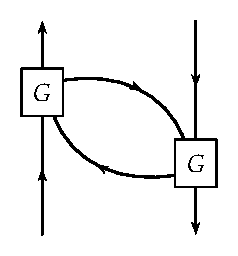
\includegraphics[width=0.28\linewidth]{pictures/4_7}
\par\end{centering}
\caption{\label{fig:4_7}粒子-空穴情形下的极化图}
\end{figure}

认识到这一点后，我们现在可以将方程\ref{eq:4.94}转换为模型$ph$空间中的方程。为此，我们将投影算符$P$拆分为向模型$ph$空间投影的部分$P_{\text{M}}$以及向$ph$空间其余部分投影的部分$P_{\text{R}}$：$P=P_{\text{M}}+P_{\text{R}}$。借助我们已经使用过的
Feshbach 投影算符形式体系 \cite{Fe62} {[}参见式 \ref{eq:4.80} 和 \ref{eq:4.81}{]}，消去方程\ref{eq:4.94}中模型空间之外的成分，即导出一个模型空间中的
TDA 方程。其中出现的有效相互作用可以按$G$矩阵展开到二阶。来自式\ref{eq:4.96}的项示于图 \ref{fig:4_8}，应当注意到对中间态线的求和仅遍历未包含在模型空间中的态。现实的计算
\cite{BK69,KBB70} 表明，包含极化图（图 \ref{fig:4_7}）具有重要效应：不包含它的 RPA 计算（见第
8 章）会给出虚数解，而极化项的贡献使解稳定下来。正如在第 8 章中更详细讨论的，其原因在于 RPA 过高估计了基态关联，必须引入极化项或屏蔽项来降低这些关联。通过这些评述，我们结束对微观有效相互作用的探讨，并在下一节中转向其唯象对应物。

\begin{figure}[H]
\begin{centering}
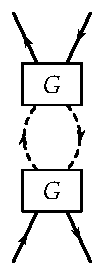
\includegraphics[width=0.28\linewidth]{pictures/4_8}
\par\end{centering}
\caption{\label{fig:4_8}模型 $ph$ 空间中对 $V_{\text{eff}}$ 的二阶贡献。虚线中间态线表示求和仅遍历未包含在模型空间中的态}
\end{figure}


\section{唯象有效相互作用}

\subsection{一般评述}

在第 4.3 节中，我们看到了如何从微观上定义有效核力，以及在实际中计算它们并获得与实验定量吻合的结果是多么困难。因此从核物理发展的早期起，人们就采用了唯象核力，其中包含若干通过拟合实验数据确定的拟合参数（fit
parameters）。在许多情形下，这种做法被证明是极其成功的，仅使用一次性选定并对所有体系通用的少数几个参数，就能解释涵盖甚广的核质量范围内的丰富实验数据。因此，至今仍然缺乏能够令人满意地解释这些唯象核力成功的微观理论，就更显得令人遗憾。

当然，在核物理问题中应用过的唯象相互作用数量极其庞大，每一种相互作用都针对特定问题而使用，其有效性和成功程度大相径庭。给出一个全景图超出了本书的范围，我们将把讨论限制在某些基本性质上，并仅介绍最成功的典型范例。大多数唯象力是专为特定目的构造的，例如用于
Hartree–Fock 计算（见第 5 章），用于计算核自洽场以及核的整体性质（如结合能和饱和密度）；其它相互作用则作为价核子之间或粒子与空穴之间的有效核力（见第
4.3 节）。因此，即使这些不同类型的相互作用在数学结构上看起来非常相似，我们在比较它们时也必须格外审慎。

正如我们在上一节所讨论的，有效相互作用是在特定的壳模型组态空间（即\textbf{模型空间}）中使用的。因此我们必然预期有效相互作用对该空间具有某种依赖性，也就是说，对于不同尺度的模型空间必须选取不同的相互作用。正如我们所见，微观定义的有效相互作用始终是依赖于能量的，而在唯象核力中大部分时间没有显式的能量依赖性，通常将所有这些依赖性归结为一个可变的强度参数就足够了。

显而易见，我们更倾向于将有效相互作用的解析形式选得尽可能简单。例如，人们常常假设有效相互作用遵循与裸核子-核子相互作用相同的\textbf{不变性原理}（见第
4.2 节）。这当然并不总是正确的。例如，我们应当预期描述从裸核子-核子相互作用过渡到有效相互作用的重正化过程依赖于体系的实际密度，也就是说，在体系内部与在表面及外部区域得到的力是不同的。对于在固定势阱中的壳模型计算，我们不应期望剩余相互作用具有平移不变性。

我们知道\textbf{核力的力程}相当短。在第 4.3 节中我们看到，对于有效 $G$ 矩阵的力程而言亦是如此。因此最简单的设想是采用\textbf{零程力}（zero-range
force），其径向依赖由 $\delta$ 函数描述。事实上，这类核力非常有用，因为它们处理极其简便，且能很好地描述许多原子核性质。然而更现实的核力需要具有有限非零的力程
\cite{AS71,Sch72b}。有限力程可以通过\textbf{动量依赖性}来模拟。为了说明这一点，我们将相对距离 $\boldsymbol{r}=\boldsymbol{r}_{1}-\boldsymbol{r}_{2}$
的函数 $V(\boldsymbol{r})$ 变换到动量空间：
\begin{equation}
\langle\boldsymbol{p}|V|\boldsymbol{p}^{\prime}\rangle=\frac{1}{(2\mathrm{\pi}\hbar)^{3}}\int\mathrm{e}^{-\frac{\mathrm{i}}{\hbar}(\boldsymbol{p}-\boldsymbol{p}^{\prime})\cdot\boldsymbol{r}}V(\boldsymbol{r})\,\mathrm{d}^{3}\boldsymbol{r}\label{eq:4.97}
\end{equation}
我们看到 $\delta$ 力在动量空间中是一个常数，而任何力程在动量空间中都表现为 $\boldsymbol{p}$ 依赖性。最简单的转动不变形式为：
\begin{equation}
(2\mathrm{\pi}\hbar)^{3}\langle\boldsymbol{p}|V|\boldsymbol{p}^{\prime}\rangle=V_{0}+V_{1}\boldsymbol{p}^{\prime2}+V_{1}\boldsymbol{p}^{2}+V_{2}\boldsymbol{p}\cdot\boldsymbol{p}^{\prime}\label{eq:4.98}
\end{equation}
在坐标空间中，这对应于动量依赖算符：
\begin{equation}
V(\boldsymbol{r})=V_{0}\delta(\boldsymbol{r})+V_{1}(\hat{\boldsymbol{p}}^{2}\delta(\boldsymbol{r})+\delta(\boldsymbol{r})\hat{\boldsymbol{p}}^{2})+V_{2}\hat{\boldsymbol{p}}\cdot\delta(\boldsymbol{r})\hat{\boldsymbol{p}}\label{eq:4.99}
\end{equation}

有效核力通常依赖于密度 $\rho(\boldsymbol{r})$。例如，如果我们考虑 $G$ 矩阵的表达式 (4.39)，这种\textbf{密度依赖性}便很容易理解：求和的能量范围取决于
Fermi 能，而 Fermi 能本身就是密度的函数。同样容易看出，进入有效相互作用定义的投影算符 $Q$ {[}见式 (4.40)
与 (4.77){]} 可以表示为非局域密度，这是密度依赖性的另一个来源。另一类效果出奇良好的简单形式是\textbf{可分离双体相互作用}，即可以表示为乘积形式（或乘积之和）的核力，其中每个因子仅作用于两个粒子中的一个。

\subsection{简单中心力}

存在大量仅使用中心部分 (4.20) 但径向依赖 $V(r)$ 不同的相互作用。常用的简单势包括例如 Yukawa 势 (4.33)
或：
\begin{align}
V(r) & =-V_{0}\mathrm{e}^{-r^{2}/r^{2}_{0}} & \text{（Gauss 势）}\label{eq:4.100}\\
V(r) & =-V_{0}\frac{\mathrm{e}^{-r/r_{0}}}{1-\mathrm{e}^{-r/r_{0}}} & \text{（Hulthén 势）}\label{eq:4.101}\\
V(r) & =-V_{0}\delta\left(\frac{\boldsymbol{r}}{r_{0}}\right) & \text{（接触势）}\label{eq:4.102}
\end{align}
调节势阱深度 $V_{0}$ 与力程 $r_{0}$ 以拟合实验数据。通常取 $V_{0}\simeq50\,\text{MeV}$
以及 $r_{0}\simeq1\sim2\,\text{fm}$（$\pi$ 介子的 Compton 波长为 $1.4\,\text{fm}$）。

对于式 (4.20) 中依赖于 $r$ 的系数 $V(r)$，通常假定它们具有相同的径向依赖，仅调节其强度与符号以拟合经验数据。在此我们不打算讨论这些混合方案中哪一种是最优的，而仅在表
\ref{tab:=004EA4=006362=006DF7=005408=007CFB=006570} 中给出文献中常用的若干交换混合系数。

\begin{table}[H]
\begin{centering}
\caption{\label{tab:=004EA4=006362=006DF7=005408=007CFB=006570}交换混合系数}
\par\end{centering}
\centering{}%
\begin{tabular}{lcccc}
\hline 
混合类型 & $a_{et}$ & $a_{es}$ & $a_{ot}$ & $a_{os}$\tabularnewline
\hline 
Wigner & 1 & 1 & 1 & 1\tabularnewline
Kurath \cite{Ku56,SW66} & 1 & 0.6 & -0.6 & -1\tabularnewline
Serber \cite{HS57} & 1 & 1 & 0 & 0\tabularnewline
Rosenfeld \cite{EF57} & 1 & 0.6 & -0.34 & -1.78\tabularnewline
Ferrel–Visscher \cite{VF57} & 1 & 0.634 & -0.366 & 0\tabularnewline
Soper \cite{So57} & 1 & 0.46 & 0.14 & -0.4\tabularnewline
Gillet \cite{GGS66} I & 1 & 0.6 & -0.6 & 0.6\tabularnewline
\cite{GGS66} \}II & 1 & 0.4 & -0.2 & 0.2\tabularnewline
\hline 
\end{tabular}
\end{table}


\subsection{Skyrme 相互作用}

这种类型的力最初由 Skyrme \cite{Sk56,Sk59} 提出，用于 Hartree–Fock 计算。为了获得核物质的饱和性质，Skyrme
考虑了一个包含两体力和三体力的有效 Hamilton 量：
\begin{equation}
V=\sum_{i<j}v(i,j)+\sum_{i<j<k}v(i,j,k)\label{eq:4.103}
\end{equation}
三体项取为纯零程形式：
\begin{equation}
v(1,2,3)=t_{3}\delta(\boldsymbol{r}_{1}-\boldsymbol{r}_{2})\delta(\boldsymbol{r}_{2}-\boldsymbol{r}_{3})\label{eq:4.104}
\end{equation}
而两体项是动量空间中的短程展开，其形式类似于式 (4.99)：
\begin{align}
v(1,2) & =t_{0}(1+x_{0}P^{\sigma})\delta(\boldsymbol{r}_{1}-\boldsymbol{r}_{2})+\frac{1}{2}t_{1}[\delta(\boldsymbol{r}_{1}-\boldsymbol{r}_{2})\boldsymbol{k}^{2}+\boldsymbol{k}^{\prime2}\delta(\boldsymbol{r}_{1}-\boldsymbol{r}_{2})]\nonumber \\
 & \quad+t_{2}\boldsymbol{k}^{\prime}\cdot\delta(\boldsymbol{r}_{1}-\boldsymbol{r}_{2})\boldsymbol{k}+\mathrm{i}W_{0}(\boldsymbol{\sigma}_{1}+\boldsymbol{\sigma}_{2})\cdot[\boldsymbol{k}^{\prime}\times\delta(\boldsymbol{r}_{1}-\boldsymbol{r}_{2})\boldsymbol{k}]\label{eq:4.105}
\end{align}
其中动量算符定义为：
\begin{equation}
\boldsymbol{k}=\frac{1}{2\mathrm{i}}(\boldsymbol{\nabla}_{1}-\boldsymbol{\nabla}_{2})\label{eq:4.106}
\end{equation}
它向右侧作用；而
\begin{equation}
\boldsymbol{k}^{\prime}=-\frac{1}{2\mathrm{i}}(\boldsymbol{\nabla}^{\prime}_{1}-\boldsymbol{\nabla}^{\prime}_{2})\label{eq:4.107}
\end{equation}
向左侧作用。相互作用中的六个参数 $t_{0},t_{1},t_{2},t_{3},x_{0},W_{0}$ 必须针对核物质与有限核性质拟合。最后带有
$W_{0}$ 的项表示一个两体自旋-轨道相互作用，正如在第 5 章中将看到的，它在平均场中产生了通常的壳模型单粒子自旋-轨道势。对于自旋饱和的偶偶核，三体项
(4.104) 证明等价于一个密度依赖的双体相互作用\footnote{对于无自旋饱和的体系，这一等价性不再成立。在此类情形下，Skyrme 力中的三体项 (4.107) 是纯局域且排斥的，倾向于自旋平行排列，即核铁磁性。这与观测到的核自旋饱和与配对性质相矛盾。这一困难可以通过采用形如
(4.109) 的密度依赖双体相互作用 \cite{BJS75} 或在三体项中引入非局域性 \cite{ON78} 来避免。}：
\begin{equation}
V_{\rho}(1,2)=\frac{1}{6}t_{3}(1+P^{\sigma})\delta(\boldsymbol{r}_{1}-\boldsymbol{r}_{2})\rho\left(\frac{1}{2}(\boldsymbol{r}_{1}+\boldsymbol{r}_{2})\right)\label{eq:4.109}
\end{equation}

这种密度依赖项也可以看作微观有效相互作用中 $\rho$ 依赖性的唯象表现。这种解释优于认为 Skyrme 力包含三体相互作用的观点，因为我们知道核内的三体相互作用是相当微弱的。过去十多年中，这种力之所以获得如此巨大的重要性，基本上有三个原因：

(i) Vautherin 与 Brink \cite{VB72}（见第 5 章）能够用一套合理的参数复现全元素周期表范围内的结合能，并同时给出正确的核半径。这对于通常不依赖于密度的核力来说此前是无法做到的。

(ii) Negele 与 Vautherin \cite{NV72} 给出了这种核力与前几节所讨论的更基本的 $G$ 矩阵之间的微观联系。

(iii) 该核力的数学形式极其简捷，$\delta$ 函数使各类计算得到了极大的简化。

存在最初由 Moszkowski \cite{Mo70} 提出的类似相互作用，即所谓的\textbf{修正 $\delta$ 相互作用}（modified
$\delta$-interactions, MDI）。它们与 Skyrme 相互作用的区别在于省去了 $t_{2}$ 项和自旋-轨道耦合力，并且具有不同的密度依赖形式（$\sim\rho^{\sigma}$，其中
$\sigma<1$）\footnote{核物质不可压缩性与密度依赖指数 $\sigma$ 之间存在强烈的关联 \cite{CS72}。}。

\subsection{Gogny 相互作用}

尽管 Skyrme 相互作用取得了巨大成功，但人们指出，零程力可能无法模拟现实有效相互作用的长程甚至中程部分。特别是，目前版本的 Skyrme
力无法恰当描述核内的对关联（见第 6 章），因此 Gogny \cite{Go75b} 将 Skyrme 力中的 $t_{0},t_{1},t_{2}$
部分替换为两个带有自旋-同位旋交换混合的 Gauss 函数之和\footnote{Brink 与 Booker \cite{BB67} 最初使用了这一形式；类似密度依赖的有效相互作用在 \cite{Kr70,ZR71,RPS72,LMV73,RBP77}
中亦被广泛采用。}，得到：
\begin{align}
V(1,2) & =\sum^{2}_{i=1}\mathrm{e}^{-(\boldsymbol{r}_{1}-\boldsymbol{r}_{2})^{2}/\mu^{2}_{i}}(W_{i}+B_{i}P^{\sigma}-H_{i}P^{\tau}-M_{i}P^{\sigma}P^{\tau})\nonumber \\
 & \quad+\mathrm{i}W_{0}(\boldsymbol{\sigma}_{1}+\boldsymbol{\sigma}_{2})\cdot[\boldsymbol{k}^{\prime}\times\delta(\boldsymbol{r}_{1}-\boldsymbol{r}_{2})\boldsymbol{k}]\nonumber \\
 & \quad+t_{3}(1+P^{\sigma})\delta(\boldsymbol{r}_{1}-\boldsymbol{r}_{2})\rho^{1/3}\left(\frac{1}{2}(\boldsymbol{r}_{1}+\boldsymbol{r}_{2})\right)\label{eq:4.110}
\end{align}
通过拟合有限核性质和核物质性质确定其参数（见表 \ref{tab:Gogny=00529B=0053C2=006570}）。

\begin{table}[H]
\begin{centering}
\caption{\label{tab:Gogny=00529B=0053C2=006570}Gogny 力参数（D1 参数集）}
\par\end{centering}
\centering{}%
\begin{tabular}{ccccccl}
\hline 
$i$ & $\mu_{i}\,[\text{fm}]$ & $W_{i}$ & $B_{i}$ & $H_{i}$ & $M_{i}\,[\text{MeV}]$ & 其他参数\tabularnewline
\hline 
1 & 0.7 & -402.4 & -100.0 & -496.2 & -23.56 & $W_{0}=+115\,[\text{MeV}\cdot\text{fm}^{5}]$\tabularnewline
2 & 1.2 & -21.30 & -11.77 & 37.27 & -68.81 & $t_{3}=1350\,[\text{MeV}\cdot\text{fm}^{4}]$\tabularnewline
\hline 
\end{tabular}
\end{table}


\subsection{Migdal 力}

这种相互作用由 Migdal \cite{Mi67} 在其有限 Fermi 体系理论中提出。基于 Landau 的 Fermi 液体理论中的相互作用准粒子概念
\cite{La59}，Migdal 引入该相互作用来描述原子核中的集体激发\footnote{详尽展开这一理论将超出本书范围；读者可在第 F.7 节找到某些基本理论成分。}。

从偶偶体系的基态出发，准粒子被定义为相邻奇质量数核中的低激发态。偶偶体系的基态不包含准粒子，而激发态由准粒子占据数 $n_{\lambda}$
来表征。这些占据数发生微小改变 $\delta n_{\lambda}$ 会引起体系总能量 $E_{0}$ 的改变：
\begin{equation}
\delta E_{0}=\sum_{\lambda}\epsilon^{0}_{\lambda}\delta n_{\lambda}+\frac{1}{2}\sum_{\lambda\lambda^{\prime}}F_{\lambda\lambda^{\prime}}\delta n_{\lambda}\delta n_{\lambda^{\prime}}
\end{equation}
其中 $\epsilon^{0}_{\lambda}$ 为在没有任何其它准粒子存在时准粒子 $\lambda$ 的能量，$F_{\lambda\lambda^{\prime}}$
是所谓的准粒子相互作用。Migdal 引入了有效粒子-空穴相互作用 $F^{\omega}$ 以及有效粒子-粒子（或空穴-空穴）相互作用
$F^{\xi}$。在具有平移不变性的无限体系中，准粒子由动量 $\boldsymbol{k}$ 表征，Landau 证明了 $ph$
相互作用 $F(\boldsymbol{k},\boldsymbol{k}^{\prime})$ 由总能量 $E_{0}$ 对准粒子密度
$n(\boldsymbol{k})$ 的二阶导数给出：
\begin{equation}
F^{ph}(\boldsymbol{k},\boldsymbol{k}^{\prime})=\frac{\delta^{2}E_{0}}{\delta n(\boldsymbol{k})\delta n(\boldsymbol{k}^{\prime})}\label{eq:4.111}
\end{equation}
在 Fermi 面上这是一个精确关系。

在有限体系中，准粒子密度 $\bar{\rho}_{\lambda\lambda^{\prime}}$ 不再完全由其对角元（占据数
$n_{\lambda}$）决定，而且还包含了关于单粒子波函数 $\varphi_{\lambda}$ 形式的信息。有效相互作用此时依赖于四个指标，人们建议类比于式
(4.111)，从精确基态能量中导出这一物理量 \cite{Br71}：
\begin{equation}
F^{ph}_{psqr}=\frac{\delta E_{0}}{\delta\bar{\rho}_{qp}\delta\bar{\rho}_{rs}}\label{eq:4.112}
\end{equation}
迄今尚未严格证明这是一个精确关系。然而在截然不同的（近似）理论——小振幅极限下的含时 Hartree–Fock 理论（见第 8.5
节）中，可以导出非常类似的形式：从波函数为 Slater 行列式（即 $\rho^{2}=\rho$，见第 5.3.3 节）且总能量可表示为泛函
$E_{0}[\rho]$ 的假设出发，我们将有效 $ph$ 相互作用获得为 $E_{0}[\rho]$ 对 $\rho$
的二阶泛函导数 {[}式 (8.124){]}，正如在式 (4.112) 中一样。

从上述讨论显而易见，例如 Skyrme 力（第 4.4.3 节）不能直接与 Migdal 力相比，尽管它们在形式上非常相似。然而在近似
$\rho^{2}\simeq\rho$ 下，通过将用 Skyrme 相互作用计算出的基态能量对密度进行两次微商，可以在二者之间建立间接的联系。

与 Skyrme 力类似，Migdal 力是动量空间中的展开。然而与适于 Hartree–Fock 计算的势不同，动量平方项 $p^{2}$
并不起主要作用，因为 Migdal 力无论如何无需保证核物质饱和（它们是专为描述不同物理情景构造的）。在大多数计算中，仅考虑动量空间中的常数项就足够了，这在坐标空间中给出一个纯
$\delta$ 力。另一方面，自旋与同位旋交换混合在此非常重要，它们在粒子-粒子力和粒子-空穴力中是不同的：
\begin{equation}
V(1,2)=V_{0}\delta(\boldsymbol{r}_{1}-\boldsymbol{r}_{2})(f+f^{\prime}\boldsymbol{\tau}^{(1)}\cdot\boldsymbol{\tau}^{(2)}+g\boldsymbol{\sigma}^{(1)}\cdot\boldsymbol{\sigma}^{(2)}+g^{\prime}\boldsymbol{\sigma}^{(1)}\cdot\boldsymbol{\sigma}^{(2)}\boldsymbol{\tau}^{(1)}\cdot\boldsymbol{\tau}^{(2)})\label{eq:4.113}
\end{equation}
$V_{0}$ 是必须针对组态空间调节的强度参数（例如在 $^{208}\mathrm{Pb}$ 区域 $V_{0}=380\,\text{MeV}\cdot\text{fm}^{3}$）。Guman
与 Birbrair \cite{GB65} 提出通过常数 $f,f^{\prime}$ 的线性密度依赖来考虑核内部和外部相互作用强度的差异以及核表面的弥散性：
\begin{equation}
f=f^{\text{ex}}+(f^{\text{in}}-f^{\text{ex}})\rho(r)\label{eq:4.114}
\end{equation}
其中 $\rho(r)$ 具有 Fermi 分布的形式：
\begin{equation}
\rho(r)=\frac{1}{1+\exp[(r-R)/a]}\label{eq:4.115}
\end{equation}
附加参数 $R$ 和 $a$ 分别代表原子核的半径与弥散度。与采用密度依赖相互作用的 Hartree–Fock 计算（见第 5
章）不同，密度 (4.114) 不是自洽调节的。因此 Migdal 力破坏了平移不变性。这当然不是缺点，因为重正化过程与底层的单粒子势紧密相连，而单粒子势同样破坏了平移不变性。事实上，恰当选取有效剩余相互作用应当恢复这一不变性（见
Mikeska 与 Brenig \cite{MB69}）。由这一条件可以推导出参数 $f,f^{\prime},g,g^{\prime}$
之间的额外约束关系 \cite{NW72,NW74}。

Migdal 力已在随机相位近似框架下广泛用于计算原子核的低激发集体振动（见第 8 章）。这类振动产生的有效电荷（见第 9 章）提供了大量的实验数据，用以调节粒子-空穴与粒子-粒子力中的六个参数
$f^{\text{in}},f^{\text{ex}},f^{\prime\text{in}},f^{\prime\text{ex}}$
以及 $g,g^{\prime}$（有关细节参见 \cite{RBS73,BSK73,BER75}）。对于粒子-空穴力，Ring
与 Speth \cite{RS74a} 确定其数值为：
\begin{align}
f^{\text{in}} & =0.0685; & f^{\prime\text{in}} & =0.3315; & f^{\text{ex}} & =-2.165;\nonumber \\
f^{\prime\text{ex}} & =0.465; & g & =0.575; & g^{\prime} & =0.725\label{eq:4.116}
\end{align}
值得注意的是，这是一种未被反对称化的有效 $ph$ 力 \cite{KMS76}。它在原子核外部表现出强烈的吸引，而在原子核内部则接近于零。

\subsection{表面 δ 相互作用（SDI）}

与 Migdal 相互作用类似，表面 $\delta$ 力（Surface-Delta Interaction, SDI）被视为
Fermi 面附近粒子间的有效剩余相互作用。其主要物理思想是：核子在核内部几乎独立运动。事实上，Migdal 的剩余相互作用在核内部确实相当微弱。大部分碰撞发生在核表面，在那里
Pauli 原理失去其重要性，核子感受到强烈的吸引相互作用 \cite{GM65}。力在表面外部的行为再次变得无关紧要，因为那里的波函数具有指数衰减的尾巴，即发现核子的概率迅速趋于零。因此，将整个相互作用限制在核表面上，并定义所谓的\textbf{表面
$\delta$ 相互作用}，是一种十分有意义的物理近似：
\begin{equation}
V(1,2)=-V_{0}\delta(\boldsymbol{r}_{1}-\boldsymbol{r}_{2})\delta(|\boldsymbol{r}_{1}|-R_{0})\label{eq:4.117}
\end{equation}
$V_{0}$ 仍可按通常方式依赖于自旋和同位旋坐标 (4.20)。该力具有非常简单的几何性质。利用 $\delta$ 函数在
Legendre 多项式中的展开：
\begin{equation}
\delta(\boldsymbol{r}_{1}-\boldsymbol{r}_{2})=\frac{\delta(r_{1}-r_{2})}{r_{1}r_{2}}\sum_{l}\frac{2l+1}{4\mathrm{\pi}}P_{l}(\cos\theta_{12})\label{eq:4.118}
\end{equation}
其中 $\theta_{12}$ 为矢量 $\boldsymbol{r}_{1}$ 与 $\boldsymbol{r}_{2}$
之间的夹角，并应用球谐函数的加法定理 \cite[式 4.6.6]{Ed57}，我们得到：
\begin{equation}
V(1,2)=-V_{0}\sum_{lm}\frac{\delta(r_{1}-R_{0})}{r_{1}}Y^{*}_{lm}(\theta_{1},\varphi_{1})\frac{\delta(r_{2}-R_{0})}{r_{2}}Y_{lm}(\theta_{2},\varphi_{2})\label{eq:4.119}
\end{equation}
这是关于可分离项的无穷求和。在球对称基下，耦合到确定角动量的矩阵元变得极其简单，因为在 (4.119) 的求和中只有一项能够幸存下来。该模型力已在诸多计算中得到广泛应用
\cite{KS63,PAM66,FP67,Fa68,VPK69}。它与 Migdal 力一样被用作价核子间的有效核力。然而，将底层的组态空间扩展到多于两个主壳层以上是没有物理意义的，因为在这种情况下我们将遇到具有相同角动量量子数的能级。由于径向积分被波函数在
$r=R_{0}$ 处的值所近似，具有不同径向节点数的波函数之间没有抵消，从而导致这些能级上的粒子感受到非物理的过强相互作用。

\subsection{可分离力与多极展开}

在上一小节中我们看到，表面 $\delta$ 相互作用由于其在壳模型基中的可分离性而变得极其便于处理。如果在二次量子化中相互作用可写为如下形式（符号
$::$ 表示按式 (C.50) 意义下的正规乘积）：
\begin{equation}
V=\,:Q^{\dagger}\cdot Q:\,,\label{eq:4.120}
\end{equation}
其中
\begin{equation}
Q=\sum_{k_{1}k_{2}}q_{k_{1}k_{2}}a^{\dagger}_{k_{1}}a_{k_{2}}\label{eq:4.121}
\end{equation}
为单粒子算符，则我们称核力在\textbf{粒子-空穴方向上可分离}。当其作用于 Slater 行列式时，它产生 $ph$ 对的叠加。如果核力具有形式：
\begin{equation}
V=P^{\dagger}\cdot P\label{eq:4.122}
\end{equation}
其中
\begin{equation}
P^{\dagger}=\frac{1}{2}\sum_{k_{1}k_{2}}p_{k_{1}k_{2}}a^{\dagger}_{k_{1}}a^{\dagger}_{k_{2}}\label{eq:4.123}
\end{equation}
为对产生算符，则称该力在\textbf{粒子-粒子方向上可分离}。当其作用于 Slater 行列式时，产生 $pp$ 对的叠加。像式
(4.120) 和 (4.122) 这样简单的设想似乎很难真实地代表现实核力，然而业已证明，这类示意力在选取适当强度时的矩阵元，与从带有极化项的微观
$G$ 矩阵计算出的矩阵元量级完全一致（见第 4.3 节与附录 F.5）\cite{BK67b}。

在此我们希望进一步研究可分离性问题，并考察不包含自旋与同位旋依赖性的一般唯象有效核力。该核力仅依赖于核子之间的相对距离，因此我们可以按如下方式展开
\cite{La64}：
\begin{equation}
V(|\boldsymbol{r}_{1}-\boldsymbol{r}_{2}|)=\sum_{l}V_{l}(r_{1},r_{2})\sum_{m}Y^{*}_{lm}(\theta_{1},\varphi_{1})Y_{lm}(\theta_{2},\varphi_{2})\label{eq:4.124}
\end{equation}
其中
\begin{equation}
V_{l}(r_{1},r_{2})=2\mathrm{\pi}\int^{1}_{-1}V(|\boldsymbol{r}_{1}-\boldsymbol{r}_{2}|)P_{l}(\cos\theta_{12})\,\mathrm{d}\cos\theta_{12}\label{eq:4.125}
\end{equation}
对于 $\delta$ 力 $V=-V_{0}\delta(\boldsymbol{r})$，我们发现 $V_{l}$ 与 $l$
无关：
\begin{equation}
V_{l}(r_{1},r_{2})=-V_{0}\frac{\delta(r_{1}-r_{2})}{r_{1}r_{2}}\label{eq:4.126}
\end{equation}
在式 (4.124) 中，我们将一般的力写为了无穷项求和，其中每一项在角坐标上都是可分离的。从 $\delta$ 力的情况可以看出，对于短程力我们不能期望这种展开迅速收敛。事实上，如果我们将注意力局限在空间中
$r_{1}\simeq r_{2}\simeq r$ 的较小区域，便可以估计展开式 (4.124) 中每个成分的有效力程。函数
$P_{l}(\cos\theta_{12})$ 的主要贡献仅集中在 $0\le\theta_{12}\lesssim1/l$
的区域（图 \ref{fig:4_9}），也就是说，若势 $V(r_{12})$ 的力程相比于 $r/l$ 很大，则 $V_{l}$
(4.125) 很小；高 $l$ 分量 $V_{l}$ 的强度越大，核力的力程就越短。在零程力（$\delta$ 力）中，所有
$l$ 分量具有相同的相对权重。

\begin{figure}[H]
\begin{centering}
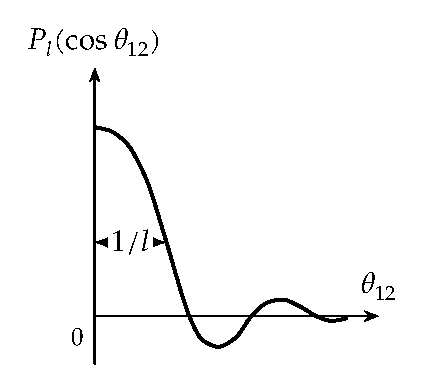
\includegraphics[width=0.42\linewidth]{pictures/4_9}
\par\end{centering}
\caption{\label{fig:4_9}\label{fig:=009636Legendre=00591A=009879=005F0F=005173=004E8E=005939=0089D2=007684=0051FD=006570}$l$
阶 Legendre 多项式作为 $\boldsymbol{r}_{1}$ 和 $\boldsymbol{r}_{2}$ 夹角
$\theta_{12}$ 的函数}
\end{figure}

现在我们回到可分离性问题。由于 $V_{l}(r_{1},r_{2})$ 的径向依赖性，一般的核力 (4.124) 以及 $\delta$
力 (4.126) 并不是可分离的。另一方面，如果假设相互作用具有如 SDI 相互作用 (4.117) 那样在表面尖锐成峰的形式，则由于附加因子
$\delta(r-R_{0})$ 的存在，它便成为可分离项之和：
\begin{equation}
V^{\text{SDI}}_{l}(r_{1},r_{2})=\frac{-V_{0}}{r_{1}}\delta(r_{1}-R_{0})\frac{1}{r_{2}}\delta(r_{2}-R_{0})\label{eq:4.127}
\end{equation}
此类形式的更普遍的可分离设想为：
\begin{equation}
V_{l}(r_{1},r_{2})=f_{l}(r_{1})f_{l}(r_{2})\label{eq:4.128}
\end{equation}
人们通常选取 $f_{l}\sim r^{l}$，并得到\textbf{多极-多极核力}（multipole–multipole
forces）：
\begin{equation}
V=-\frac{1}{2}\sum_{lm}\chi_{l}:Q^{\dagger}_{lm}Q_{lm}:\,=-\frac{1}{2}\sum_{l}\chi_{l}:Q^{\dagger}_{l}\cdot Q_{l}:\label{eq:4.129}
\end{equation}
其中 $\chi_{l}$ 是常数，$Q_{lm}$ 为多极算符：
\begin{equation}
Q_{lm}=\sum_{k_{1}k_{2}}\langle k_{1}|r^{l}Y_{lm}(\theta,\varphi)|k_{2}\rangle a^{\dagger}_{k_{1}}a_{k_{2}}\label{eq:4.130}
\end{equation}
若只考虑具有较小 $l$ 值的成分，我们就获得了\textbf{长程力}。其中最著名的是四极-四极力（quadrupole–quadrupole
force）\cite{El58,KS63}。我们在第 7 章中将看到，它可以用来以自洽的方式描述原子核的四极形变。

我们必须再次强调，这些多极力仅应被视为限制组态空间内价核子之间的有效核力。如果存在许多这样的价核子，我们可以对它们应用 Hartree–Fock
近似\footnote{在此类计算中，HF 势中的交换项 (5.43) 通常因为很小而被忽略 \cite{BK68,Ma74}。}（见第
5 章）。然而，这种针对价核子的多极力 HF 计算绝不能与针对结合能的基础 HF 计算相混淆。

展开式 (4.124) 证明对有效相互作用的\textbf{长程部分}非常有用，因为在此时函数 $V_{l}$ 对较高的 $l$
值变得很小。为了对\textbf{短程部分}获得类似的描述，人们采用另一种不同的展开。我们将把注意力限制在同类核子之间的相互作用（关于质子与中子之间短程关联的处理见第
7.5 节）。我们考察不一定局域的核力的一般表达式 (4.3)：$V(\boldsymbol{r}_{1},\boldsymbol{r}_{2},\boldsymbol{r}^{\prime}_{1},\boldsymbol{r}^{\prime}_{2})$。在局域力的情况下，我们有
$\boldsymbol{r}_{1}=\boldsymbol{r}^{\prime}_{1}$ 以及 $\boldsymbol{r}_{2}=\boldsymbol{r}^{\prime}_{2}$，展开式
(4.124) 是在变量 $\boldsymbol{r}_{1},\boldsymbol{r}_{2}$ 中进行的。现在我们改为要求
$\boldsymbol{r}_{1}=\boldsymbol{r}_{2}$ 以及 $\boldsymbol{r}^{\prime}_{1}=\boldsymbol{r}^{\prime}_{2}$，并在
$\boldsymbol{r}_{1},\boldsymbol{r}^{\prime}_{1}$ 中展开，获得类似于 (4.124)
和 (4.125) 的表达式：
\begin{align}
 & \delta(\boldsymbol{r}_{1}-\boldsymbol{r}_{2})\delta(\boldsymbol{r}^{\prime}_{1}-\boldsymbol{r}^{\prime}_{2})V(\boldsymbol{r}_{1},\boldsymbol{r}^{\prime}_{1})\nonumber \\
= & \,\delta(\boldsymbol{r}_{1}-\boldsymbol{r}_{2})\delta(\boldsymbol{r}^{\prime}_{1}-\boldsymbol{r}^{\prime}_{2})\sum_{lm}V_{l}(r_{1},r^{\prime}_{1})Y_{lm}(\theta_{1},\varphi_{1})Y^{*}_{lm}(\theta^{\prime}_{1},\varphi^{\prime}_{1})\label{eq:4.131}
\end{align}
条件 $\boldsymbol{r}_{1}=\boldsymbol{r}_{2}$ 和 $\boldsymbol{r}^{\prime}_{1}=\boldsymbol{r}^{\prime}_{2}$
已经将我们限制在短程，因为这仅在两个核子处于同一位置时才成立（这并不一定意味着 $\delta$ 力，因为我们允许非局域力）。乍看起来，展开式
(4.131) 对于短程力似乎与式 (4.124) 一样低效。然而，我们必须计算双粒子波函数的矩阵元。正如我们即将证明的，当两个粒子耦合到自旋
$I=l$ 时，(4.131) 中的第 $l$ 项才对矩阵元有贡献。对于单个 $j$ 壳层中的两个粒子而言，例如我们发现当 $I=0$
时它们的波函数具有最大的空间重叠。在此情形下，其波函数的角向部分具有以下形式：
\begin{equation}
\langle\Omega_{1}\Omega_{2}|jjI=0,M=0\rangle\propto\sum^{l}_{m=-l}(-)^{m}Y_{lm}(\Omega_{1})Y_{l,-m}(\Omega_{2})\propto P_{l}(\cos\theta_{12})\label{eq:4.132}
\end{equation}
（由于短程力的性质，我们假设仅自旋单态是重要的）。因此我们发现对于 $I=0$ 相互作用最大，此时角动量 $\boldsymbol{j}_{1}$
与 $\boldsymbol{j}_{2}$ 反平行排列；由此我们可以理解展开式 (4.131) 对于短程相互作用是有重要物理意义的。

同样，如果我们像式 (4.129) 那样将不可分离的径向项替换为可分离设想，即得到：
\begin{equation}
V_{l}(r_{1},r^{\prime}_{1})=-G_{l}r^{l}_{1}r^{\prime l}_{1}\label{eq:4.133}
\end{equation}
由此
\begin{equation}
V=-\sum_{lm}G_{l}P^{\dagger}_{lm}P_{lm}=-\sum_{l}G_{l}P^{\dagger}_{l}\cdot P_{l}\label{eq:4.134}
\end{equation}
其中
\begin{equation}
P^{\dagger}_{lm}=\frac{1}{2}\sum_{k_{1}k_{2}}\langle k_{1}|r^{l}Y_{lm}|\bar{k}_{2}\rangle a^{\dagger}_{k_{1}}a^{\dagger}_{k_{2}}\label{eq:4.135}
\end{equation}
其中 $|\bar{k}\rangle$ 为态 $|k\rangle$ 的时间反演态。在从式 (4.131) 导出式 (4.134)
时，我们必须小心处理自旋坐标 $s$，因为算符 (4.133) 在自旋空间中先验地不是可分离的。然而由于 $\delta$ 力的性质，我们总是有
$s_{1}=-s_{2}$ 以及 $s^{\prime}_{1}=-s^{\prime}_{2}$，这使得推导式 (4.134)
成为可能。

我们现在能够计算单个 $j$ 壳层中 $\delta$ 力的矩阵元，其中单粒子波函数由 $\langle\boldsymbol{r}|nljm\rangle=R_{nl}(r)\langle\Omega|ljm\rangle$
给出。我们构造具有确定角动量 $I,M$ 的对算符 $A^{\dagger}_{IM}$：
\begin{equation}
A^{\dagger}_{IM}=\frac{1}{\sqrt{2}}\sum_{m_{1}m_{2}}C^{j\;\;j\;\;I}_{m_{1}m_{2}M}a^{\dagger}_{jm_{1}}a^{\dagger}_{jm_{2}}\label{eq:4.136}
\end{equation}
并利用式 (4.124) 和 (4.126) 得到：
\begin{equation}
V_{\delta}=-\sum_{I=0,2,\ldots}V_{\delta}(I)\sum_{M}A^{\dagger}_{IM}A_{IM}\label{eq:4.137a}
\end{equation}
其中
\begin{equation}
V_{\delta}(I)=V_{0}\cdot R_{4}\frac{1}{2}\frac{1}{2I+1}|\langle j||Y_{I}||j\rangle|^{2}=\frac{V_{0}}{8\mathrm{\pi}}R_{4}\frac{(2j+1)^{2}}{2I+1}\left|C^{j\;\;\;\;\;j\;\;\;\;\;I}_{1/2\;-1/2\;0}\right|^{2}\label{eq:4.137}
\end{equation}
其中 $R_{4}$ 为径向积分：
\begin{equation}
R_{4}=\int^{\infty}_{0}\mathrm{d}r\,r^{2}R^{4}_{nl}(r)
\end{equation}
从式 (4.137) 可以看出，展开式 (4.131) 中只有第 $l$ 项进入耦合到自旋 $I=l$ 的矩阵元中。在 $\delta$
力的情形下，$V_{\delta}(I)$ 在 $I=0$ 时达到最大值，并随着 $I$ 的增加迅速衰减（表 \ref{tab:Vdelta=0076F8=005BF9=005927=005C0F}）\footnote{在 $I$ 和 $j$ 较大极限下，通过半经典展开可以发现 \cite{MJB75}：$\left|C^{j\;\;\;\;\;j\;\;\;\;\;I}_{1/2\;-1/2\;0}\right|^{2}\simeq\frac{2}{\mathrm{\pi}j}\frac{1}{\sqrt{1-(I/2j)^{2}}}$。}。因此核力
(4.134) 中最重要的部分是 $l=I=0$ 的部分。

\begin{table}[H]
\begin{centering}
\caption{\label{tab:Vdelta=0076F8=005BF9=005927=005C0F}单个 $j$ 壳层中矩阵元 $V_{\delta}(I)$
(4.137) 的相对大小}
\par\end{centering}
\centering{}%
\begin{tabular}{cccccccc}
\hline 
$V_{\delta}(I)/V_{\delta}(0)$ & $I=0$ & 2 & 4 & 6 & 8 & 10 & 12\tabularnewline
\hline 
$j=7/2$ & 1 & 0.238 & 0.117 & 0.058 & — & — & —\tabularnewline
$9/2$ & 1 & 0.242 & 0.126 & 0.075 & 0.040 & — & —\tabularnewline
$11/2$ & 1 & 0.245 & 0.131 & 0.082 & 0.053 & 0.025 & —\tabularnewline
$13/2$ & 1 & 0.246 & 0.133 & 0.087 & 0.060 & 0.038 & 0.019\tabularnewline
\hline 
\end{tabular}
\end{table}

为了避免复杂的公式，人们通常对 Condon–Shortley 相位约定（见 \cite{Ed57}）引入微小修正，即所谓的\textbf{BCS
相位约定}，并对 $m>0$ 定义：
\begin{align}
|nljm\rangle_{\text{BCS}} & =|nljm\rangle_{\text{CS}}\nonumber \\
|nlj-m\rangle_{\text{BCS}} & =(-)^{l+j-m}|nlj-m\rangle_{\text{CS}}\label{eq:BCS phases}
\end{align}
在此约定下，时间反演态 $T|k\rangle$（见式 2.45）对于 $m>0$ 具有极其简单的形式：
\begin{equation}
|\overline{nljm}\rangle=T|nljm\rangle=|nlj-m\rangle;\quad T|nlj-m\rangle=-|nljm\rangle\label{eq:4.139}
\end{equation}
式 (4.134) 的 $l=0$ 部分即为所谓的\textbf{纯配对力}（pure pairing force），它具有以下形式：
\begin{equation}
V^{p}=-G\frac{1}{4}\sum_{\begin{subarray}{c}
kk^{\prime}\\
>0
\end{subarray}}a^{\dagger}_{k^{\prime}}a^{\dagger}_{\bar{k}^{\prime}}a_{\bar{k}}a_{k}\label{eq:pure pairing force}
\end{equation}
其中 $\bar{k}$ 再次为态 $k$ 的时间反演态，求和遍历 $k,k^{\prime}>0$ 的所有取值。该核力在 BCS
形式体系内被广泛用于描述核内的短程关联（见第 6 章）。必须再次指出，它仅适用于受限的组态空间。力常数的值与该空间的大小紧密相关。将这一简单模型力进行推广以包含展开式
(4.131) 中的更高 $l$ 值是容易的，它们被称为\textbf{多极配对力}（multipole pairing forces）。它们在粒子-粒子方向上是可分离的，在配对振动的描述中扮演着重要角色（见第
8 章与 \cite{BB71,BBN74b}）。

通过将四极-四极力与纯配对力相结合，人们获得了用于重核的一个非常简单的模型力——\textbf{配对加四极模型}（pairing-plus-quadrupole
force）\cite{KS60,KS63,BK68}：
\begin{equation}
V^{QP}=-\frac{1}{2}\chi:Q^{\dagger}_{2}\cdot Q_{2}:\,-GP^{\dagger}_{0}\cdot P_{0}\label{eq:4.141}
\end{equation}
它同时考虑了最重要的长程关联与最重要的短程关联，并且处理极其简便（见第 7.4 节）。它基本上包含三个常数：$\chi$ 以及分别针对质子和中子的两个不同配对常数
$G_{p}$ 与 $G_{n}$。它同样只能应用于不大于一个主壳层的组态空间。关于 $\chi$ 和 $G$ 的实际数值参见
\cite{KS60} 或 \cite{BK68}。

\subsection{实验确定的有效相互作用}

由于从裸核子-核子力推导有效相互作用相当繁复，一些作者尝试直接根据实验数据在特定基下确定核子-核子力的矩阵元（综述见 \cite{ST76b}
和 \cite{BPO76}）。

Elliott 等人 \cite{EJM68} 利用核子-核子散射的实验相移，直接在谐振子基下导出了有效相互作用的矩阵元（Sussex
力）。以这种方式，完全避免了硬芯所带来的困难。

较不雄心勃勃但更直接的尝试是根据“简单”原子核的能谱推导特殊的矩阵元。这些核具有充分理由相信其结构仅由少数几个矩阵元决定，这些矩阵元的数目不超过观测到的能级数
\cite{Ta62}。例如我们可以取 $1f_{7/2}$ 壳层核，其中 $f_{7/2}$ 壳层与单粒子谱的其它部分被很好地隔开。人们假设在靠近具有
$N\ge20$ 和 $Z\ge20$ 的双幻芯 $^{40}\mathrm{Ca}$ 的原子核中存在许多纯 $f_{7/2}$
组态。这些能级完全由八个矩阵元 $\langle(f_{7/2})^{2}IT|V|(f_{7/2})^{2}IT\rangle$
决定，其中 $I=0,1,\ldots,7$（对于偶数 $I$ 有 $T=1$；对于奇数 $I$ 有 $T=0$）。McCullen
等人 \cite{MBZ64} 根据 $^{42}\mathrm{Sc}$ 核的能谱确定了这些矩阵元。该核在 $^{40}\mathrm{Ca}$
芯外包含一个中子和一个质子。耦合到总角动量 $I$ 给出相互作用能：
\begin{align}
V(I) & =\langle j_{1}j_{2}I|V|j_{1}j_{2}I\rangle\nonumber \\
 & =B(I,^{42}\mathrm{Sc})-B(I,^{41}\mathrm{Sc})-B(I,^{41}\mathrm{Ca})+B(I,^{40}\mathrm{Ca})\label{eq:4.142}
\end{align}
其中 $B$ 分别为 $^{42}\mathrm{Sc}$ 中自旋为 $I$ 的能级以及其它核基态的实验结合能。利用这些矩阵元，可以相当好地复现具有更多价核子的其它
$f_{7/2}$ 核的许多能级与电磁跃迁性质。然而也遇到了具有更复杂结构（例如 $^{40}\mathrm{Ca}$ 芯中的空穴）的能级，且目前尚不清楚它们在多大程度上与纯
$f_{7/2}$ 组态发生混合。

Schiffer \cite{Sch71b,Sch72b} 以及 Molinari 等人 \cite{MJB75} 对许多这类具有纯组态的简单核进行了更为普遍的研究，其中一个核子处于壳层
$j_{1}$，另一个核子处于壳层 $j_{2}$。角动量的耦合产生自旋满足 $|j_{1}-j_{2}|\le I\le j_{1}+j_{2}$
的多重态。相互作用导致了多重态的能级分裂。为了比较不同的多重态，适宜的做法不是直接绘制 $V(I)$（式 4.137）随 $I$
的变化，而是绘制无量纲比值 $V(I)/\bar{V}$ 作为“重叠角”$\theta_{12}$的函数，其中 $\bar{V}$
是平均双体相互作用能：
\begin{equation}
\bar{V}=\frac{\sum_{I}(2I+1)V(I)}{\sum_{I}(2I+1)}\label{eq:4.143}
\end{equation}
该角度是两价核子经典轨道之间的夹角：
\begin{equation}
\cos\theta_{12}=\frac{\boldsymbol{j}_{1}\cdot\boldsymbol{j}_{2}}{|j_{1}||j_{2}|}=\frac{I(I+1)-j_{1}(j_{1}+1)-j_{2}(j_{2}+1)}{2[j_{1}(j_{1}+1)]^{1/2}[j_{2}(j_{2}+1)]^{1/2}}\label{eq:4.144}
\end{equation}
它度量了两个单粒子波函数的空间重叠。在此类曲线图（图 \ref{fig:4_10}）中，许多不同核的数据点几乎落在同一条曲线上。例如我们给出了两个价核子处于同一轨道时的实验曲线（图
\ref{fig:4_10}a），并将它们与纯 $\delta$ 力的对应理论值（图 \ref{fig:4_10}b）进行比较。对于全同粒子（$T=1$），我们再次发现绝对相互作用矩阵元在
$\theta_{12}=180^{\circ}$ 处最强，即对应于自旋反平行排列（$I=0$），且随着角度减小而迅速下降。对于非全同粒子（$T=0$），相互作用在
$\theta_{12}=0$ 处（即自旋平行排列）同样升高。对于全同粒子，这种构型被 Pauli 原理所禁戒。这体现了短程力要求波函数具有大空间重叠的事实，表明
$\delta$ 型有效相互作用能够定性地再现“实验确定的”矩阵元。然而定量比较 \cite{Sch72b,GSZ74,AEE78}
表明，为了再现奇奇核的性质，还需要引入长程分量。这种长程部分的物理起源目前尚未被完全理解。关于这一观点的深入讨论参见 \cite{Mo76c}。

\begin{figure}[H]
\begin{centering}
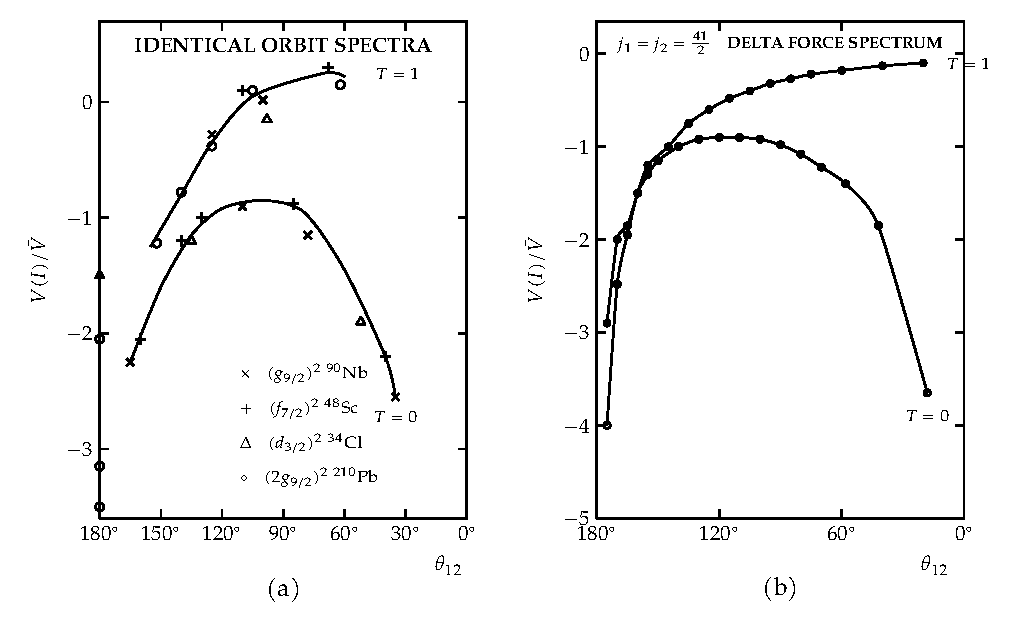
\includegraphics[width=0.78\linewidth]{pictures/4_10}
\par\end{centering}
\caption{\label{fig:4_10}相对相互作用矩阵元 $V(I)/\bar{V}$ 作为重叠角 $\theta_{12}$ 的函数。(a)
四个原子核的实验值；(b) $j_{1}=j_{2}=41/2$ 纯 $\delta$ 力谱（引自 \cite{AS71}）}
\end{figure}


\section{结论}

在本章的第二节中，我们讨论了核子之间的裸相互作用。我们首先限制了它们的解析形式，指出了它们必须服从若干不变性原理。众所周知，核子-核子相互作用的长程部分由单
$\pi$ 介子交换给出；在较短距离下，双 $\pi$ 介子交换以及更重的介子交换开始变得重要。我们没有详述此类研究的最新进展，因为微观裸核子-核子力在核物理中本身构成了一个涉及中能和高能物理的独立学科
\cite{BJ76a}。我们讨论了若干更为传统的唯象设想（通常包含 40 到 50 个拟合参数），它们实现了对核子-核子散射实验数据的完美再现。然而，这种拟合仅向我们提供了关于核力在能壳上（on-shell）行为的信息，而进入多核子体系的离壳（off-shell）部分仍然是不确定的（参见例如
\cite{SS76}）。然而三体计算表明，目前常用的双体相互作用（如 Hamada–Johnston 势或 Reid 软芯势）在离壳行为上彼此差异并不显著。因此我们拥有的唯象裸核子-核子势实际上是相当可靠的。

然而，这些势具有在短距离处强烈排斥的不便特征，因此无法直接应用于核结构计算。多体理论告诉我们应当使用有效力而非裸相互作用，前者实质上是对后者高阶效应的无穷求和。这一步骤不仅以自洽的方式计入了高阶多体效应，而且同时摆脱了硬芯带来的发散困难，因为事实证明有效相互作用是性质优良的。在下一章中我们将看到，有效相互作用概念的应用在计算核基态性质方面取得了相当大的成功，尽管该领域最前沿的纯微观计算（自洽地考虑了三体关联
\cite{KLZ78}）仍未能与实验结合能达成定量的绝对吻合。在所有其它计算中，唯象方法均在某一步骤中被引入。尽管如此，我们可以说该理论对于核基态性质给出了极好的结果。

对于价核子之间有效核力的情形，现状则远没有那么令人满意。例如，在双粒子模型空间内采用唯象双体力进行的壳模型计算能够很好地复现例如 $^{18}\mathrm{O}$
的低激发能谱，我们本可以期望这种成功能够从微观上计算两价核子间有效核力来得到证明。不幸的是，这些尝试仅取得了部分的成功，并表明在相互作用微扰展开的某一阶段与实验达成良好吻合之后，进一步包含更高阶展开项反而会使结果重新恶化。直到目前，在中间阶段达成吻合的原因仍未得到彻底解释。

在这些在数值上极为复杂却仅取得中等成功的微观有效相互作用理论之后，我们在第 4.4 节中转向了唯象有效核力的处理。在那里的情况是相当令人满意的。存在若干唯象设想，它们在解释远多于其拟合参数数量的丰富核实验数据方面取得了极大的成功。其中之一是
Skyrme 力，其在描述核基态性质方面的巨大成功将在下一章中详细讨论。对于核结构计算，我们必须提及非常简捷却高度成功的配对加四极力。在铅同位素区域，准粒子概念似乎工作得非常出色，利用
Migdal 力进行的大量计算所展现的惊人成功充分证明了这一点。像表面 $\delta$ 力这样的简单相互作用，其表现同样出人意料地良好。鉴于它们所取得的巨大成功，从微观视角给出理论解释，显然是一项艰巨却极具挑战性与吸引力的重要任务。



\chapter{Hartree-Fock方法\label{chap:Hartree-Fock=0065B9=006CD5}}

\section{引言}

唯象壳模型的成功说明了核子确实是在一个所有核子形成的平均势中运动的。现在的问题是如何从如下两体相互作用中提取出这么一个单粒子势。

\[
V(1,\dots,A)=\sum^{A}_{i<j=1}V(i,j)\simeq\sum^{A}_{i=1}V(i)
\]

当然，从两体相互作用中提取出的单粒子势和到现在为止我们使用的单粒子势有何异同也是值得探究的。之后我们将会说明，通过把Slater行列式作为变分法的试探波函数，我们可以得到两体相互作用的单粒子势。

在\ref{sec:=0053D8=005206=00539F=007406}中，我们将会讨论普遍的变分原理——在接下来的章节中它势十分重要的。在\ref{sec:Hartree-Fock=0065B9=007A0B=007684=005BFC=0051FA}我们会详细讨论Hartree-Fock方法。在\ref{sec:=004E00=004E2A=0053EF=0089E3=006A21=00578B}我们会对一个非常简单的模型应用Hartree-Fock方法。在\ref{sec:Hartree-Fock=0065B9=006CD5=004E0E=005BF9=0079F0=006027}我们讨论了Hartree-Fock方法和对称性的关系，在\ref{sec:Hartree-Fock=0065B9=006CD5=004E0E=005BC6=005EA6=004F9D=008D56=0076F8=004E92=004F5C=007528}我们提出了密度依赖力的Hartree-Fock理论。

\section{变分原理\label{sec:=0053D8=005206=00539F=007406}}

Schrödinger方程为：
\begin{equation}
H|\Psi\rangle=E|\Psi\rangle\label{eq:schrodinger equation}
\end{equation}

它等价于变分法：
\[
\delta E[\Psi]=0
\]

这里：
\[
E[\Psi]=\frac{\langle\Psi|H|\Psi\rangle}{\langle\Psi|\Psi\rangle}
\]

由此得到：
\begin{equation}
\langle\delta\Psi|H-E|\Psi\rangle+\langle\Psi|H-E|\delta\Psi\rangle=0\label{eq:delta_E}
\end{equation}

由于一般来讲$|\Psi\rangle$是一个复数函数，我们可以对实部和虚部分别变分，这等价于对$|\delta\Psi\rangle$和$\langle\delta\Psi|$独立变分。为了看出这一点，我们利用\ref{eq:delta_E}对任意无穷小变换$|\delta\Psi\rangle$都成立。我们把$|\delta\Psi\rangle$替换为$\mathrm{i}|\delta\Psi\rangle$即可得到：
\[
-\mathrm{i}\langle\delta\Psi|H-E|\Psi\rangle+\mathrm{i}\langle\Psi|H-E|\delta\Psi\rangle
\]

同\ref{eq:delta_E}联立，我们即可发现：
\[
\langle\delta\Psi|H-E|\Psi\rangle=0
\]

当然我们同时还能发现这一方程的共轭。由于$|\delta\Psi\rangle$是任意的，上述方程就等价于本征值问题\ref{eq:schrodinger equation}。

变分法的近似来自于$|\Psi\rangle$被限制在一些简单的试探波函数组成的线性空间上。只要真实波函数没有在这个线性空间里，最小值解就不是真正的本征态，而仅仅是一个近似。变分法非常适合用来找到基态，因为对于任意试探波函数，我们可以有：
\begin{equation}
E[\Psi]\geq E_{0}\label{eq:variational principle for g.s.}
\end{equation}

因此$E_{0}$是变分计算的下确界。为了证明这一点，我们把试探波函数表示成一系列Hamilton量精确解的线性组合：
\[
|\Psi\rangle=\sum^{\infty}_{n=0}a_{n}|\Psi_{n}\rangle
\]

这里：
\[
H|\Psi_{n}\rangle=E_{n}|\Psi_{n}\rangle
\]

这导致：
\[
E[\Psi]=\frac{\sum_{nn^{\prime}}a^{*}_{n}a_{n}E_{n}\delta_{nn^{\prime}}}{\sum_{n}|a_{n}|^{2}}\geq\frac{\sum_{n}|a_{n}|^{2}E_{0}}{\sum_{n}|a_{n}|^{2}}=E_{0}
\]

这就证明了\ref{eq:variational principle for g.s.}。在基态能量非简并的情况下，当且仅当$n\neq0$的系数全部为零时，即$|\Psi\rangle$正比于$|\Psi_{0}\rangle$时，等号成立。如果我们对第一激发态感兴趣，我们就需要在正交于$|\Psi_{0}\rangle$的子空间内变分，也就是对所有$a_{0}=0$的波函数$|\Psi\rangle$变分。在这个子空间中，$|\Psi_{1}\rangle$的能量最小。为了得到$|\Psi_{1}\rangle$，我们要在$\langle\Psi_{1}|\Psi_{0}\rangle=0$的限制条件下变分。原则上我们可以像这样继续计算出整个能谱。

然而实际上，我们并不知道精确的$|\Psi_{0}\rangle$。由于我们是在一个Hilbert空间的子空间上做变分，因此只能得到一个近似的基态$|\Phi_{0}\rangle$。为了计算第一激发态$|\Psi_{1}\rangle$的近似$|\Phi_{1}\rangle$，我们必须在变分时加上$|\Phi_{1}\rangle$与$|\Phi_{0}\rangle$正交的条件：
\[
\langle\Phi_{1}|\Phi_{0}\rangle=0
\]

对于第二激发态，我们必须加上两个条件：
\[
\langle\Phi_{2}|\Phi_{1}\rangle=0\quad\text{和}\quad\langle\Phi_{2}|\Phi_{0}\rangle=0
\]

这些条件通过拉格朗日乘子法处理。可以看出，随着激发态越来越高，这一方法迅速变得非常复杂，因此这一方法主要用于处理基态。当然，有时由于对称性的存在这些条件非常容易满足，例如不同的态具有不同的角动量量子数的时候。我们将在\ref{chap:=0063A8=005E7F=007684=005355=007C92=005B50=006A21=00578B=00FF08HFB=007406=008BBA=00FF09}计算出整个转动谱——转动谱中所有的能级的计算都和基态一样简单。

我们已经证明，对于特定的试探波函数，由之计算出来的基态能量总是大于等于真实的基态能量，并且总是一个极值。除此之外我们还需要确定这个极值是极小值，为此我们需要计算能量泛函的二阶泛函导数，实际计算中就是对特定参数的二阶导。在Hartree-Fock或者Hartree-Fock-Bogoliubov理论\ref{chap:=0063A8=005E7F=007684=005355=007C92=005B50=006A21=00578B=00FF08HFB=007406=008BBA=00FF09}中，我们将要再次提到这一点。

为了确定哪一组试探波函数更好，我们有两个判断标准：
\begin{enumerate}
\item 如果某一组试探波函数是另一组的子集，那么更大的一组更好，因为它一定能得到另一组得到的极小值。
\item 由于精确的能量$E_{0}$是一个下界，我们期望两组试探波函数中得到的能量更低的一组更好。
\end{enumerate}
然而，这两个标准都不是绝对的。事实上可以找到一些违背这两个原则的例子。

最后，我们需要注意，变分原理仅仅对\ref{eq:schrodinger equation}这样的线性的本征值问题成立。在Hamilton量本身依赖于波函数时，我们必须非常小心。

\section{Hartree-Fock方程的导出\label{sec:Hartree-Fock=0065B9=007A0B=007684=005BFC=0051FA}}

\subsection{试探波函数的选取\label{subsec:=008BD5=0063A2=006CE2=0051FD=006570=007684=009009=0053D6}}

考虑到壳模型对原子核的很多性质都给出了定性的解释，我们可以假设存在一个平均单粒子势（Hartree-Fock势）：
\[
H^{\text{HF}}=\sum^{A}_{i=1}h(i)
\]

其能量最低的本征函数是真实基态波函数的一种近似。这一波函数$\Phi(1\dots A)$正如在\ref{chap:=0058F3=006A21=00578B}提到的，是Slater行列式：
\[
|\text{HF}\rangle=|\Phi(1\dots A)\rangle=\prod^{A}_{i=1}a^{\dagger}_{i}|\rangle
\]

这里费米算符$a^{\dagger}_{k}$，$a_{k}$是单粒子波函数$\varphi_{k}$对应的产生湮灭算符，它们本身就是单粒子Hamilton量$h$的本征函数：
\[
h(i)\varphi_{k}(i)=\varepsilon_{k}\varphi_{k}(i),\quad i=(\boldsymbol{r}_{i},s_{i},t_{i})
\]

正如我们在\ref{sec:=00591A=004F53=0095EE=009898=007684=0058F3=006A21=00578B=0065B9=006CD5}中看到的，如果我们让$|\text{HF}\rangle$占据了能量最低的$A$个单粒子能级，我们就可以得到最低的本征能量$H^{\text{HF}}$。接下来，我们用字幕$i,j$（空穴态）来表示$|\text{HF}\rangle$中的占据态，用$m,n$（粒子态）表示未占据态。如果我们没有区分是占据还是非占据，我们用$k,l,p,q$表示。

波函数$\varphi_{k}(\boldsymbol{r},s,t)$是单粒子Hamilton量$h$的本征态$|k\rangle$的坐标表象波函数。一般来讲，我们考虑的是一组任意正交完备的单粒子波函数$\{\chi_{l}\}$（例如球谐振子波函数）构成的组态空间。函数$\varphi_{k}$可以在这组基上展开：
\[
\varphi_{k}=\sum_{l}D_{lk}\chi_{l}
\]

如果我们对每一个波函数$\chi_{l}$都定义一个相应的费米产生湮灭算符$c^{\dagger}_{l}$，$c_{l}$，我们可以简单的把算符$a^{\dagger}_{k}$用$c^{\dagger}_{l}$表示：
\begin{equation}
a^{\dagger}_{k}=\sum_{l}D_{lk}c^{\dagger}_{l}\label{eq:transformation of create operator}
\end{equation}

由于$\{\varphi_{k}\}$和$\{\chi_{l}\}$都是正交完备的，变换矩阵$D$必须是酉的：
\begin{equation}
D^{\dagger}D=DD^{\dagger}=1\label{eq:unitary condition of D}
\end{equation}

这也保证了算符$(a^{\dagger}_{k},a_{k})$和$(c^{\dagger}_{l},c_{l})$都分别遵循费米对易关系。

正如在\ref{sec:Slater=00884C=005217=005F0F=007684=005355=007C92=005B50=005BC6=005EA6=0077E9=009635}中讨论的，Slater行列式$\Phi$和一组单粒子基$\varphi_{k}$之间没有一一对应的关系。任意不混合空穴态和粒子态的酉变换都不改变$\Phi$（至少在不考虑相位的意义上）。

因此，更方便的代表Slater行列式$|\Phi\rangle$的方式是用对应的单粒子密度矩阵：
\[
\rho_{ll^{\prime}}=\langle\Phi|c^{\dagger}_{l^{\prime}}c_{l}|\Phi\rangle
\]

从\ref{eq:transformation of create operator},\ref{eq:unitary condition of D}可以得到：
\[
\rho_{ll^{\prime}}=\sum_{kk^{\prime}}D_{lk}D^{*}_{l^{\prime}k^{\prime}}\langle\Phi|a^{\dagger}_{k^{\prime}}a_{k}|\Phi\rangle=\sum^{A}_{i=1}D_{li}D^{*}_{l^{\prime}i}
\]

这里第二个等号是因为$\rho$在$a^{\dagger}_{k}$，$a_{k}$这组基下是对角的，并且本征值对于空穴态是$1$，对于粒子态是$0$。$\rho$的迹恰好等于粒子数。

正如我们在\ref{sec:Slater=00884C=005217=005F0F=007684=005355=007C92=005B50=005BC6=005EA6=0077E9=009635}看到的，Slater行列式$\Phi$和单粒子密度矩阵$\rho$之间存在一一映射。Slater行列式的单粒子密度矩阵$\rho$可以通过他们的本征值是$0$或$1$来表征，也就是：
\[
\rho^{2}=\rho
\]

因此$\rho$就是单粒子波函数空间中投影到空穴态$\varphi_{i}$张成的子空间的投影算符。

同样的，我们可以定义投影算符$\sigma$：
\[
\sigma=1-\rho
\]

它投影到粒子态$\varphi_{m}$上。

Hartree-Fock方法可以如下定义：我们考虑有$A$个任意的正交单粒子波函数$\varphi_{i}$的Slater行列式组成的试探波函数集合，在这组集合上最小化能量。与之等价的陈述是我们考虑所有单粒子密度矩阵具有性质$\rho^{2}=\rho$和$\mathop{\text{Tr}}\rho=A$的波函数。

我们在接下来的章节中可以看到，这一变分过程能让我们得到单粒子算符$H^{\text{HF}}$
\begin{comment}
不是很确定能不能真得到，原文只说了有可能性。
\end{comment}
。

\subsection{Hartree-Fock能量}

在我们真正做变分以得到HF波函数之前，我们必须计算HF能量：
\[
E^{\text{HF}}=\langle\Phi|H|\Phi\rangle
\]

我们从多体Hamilton量$H$开始，把它用二次量子化的形式表示出来即有\ref{chap:=004E8C=006B21=0091CF=005B50=005316}：
\[
H=\sum_{l_{1}l_{2}}t_{l_{1}l_{2}}c^{\dagger}_{l_{1}}c_{l_{2}}+\frac{1}{4}\sum_{l_{1}l_{2}l_{3}l_{4}}\bar{v}_{l_{1}l_{2},l_{3}l_{4}}c^{\dagger}_{l_{1}}c^{\dagger}_{l_{2}}c_{l_{4}}c_{l_{3}}
\]

这里：
\[
\bar{v}_{l_{1}l_{2},l_{3}l_{4}}=v_{l_{1}l_{2}l_{3}l_{4}}-v_{l_{1}l_{2}l_{4}l_{3}}
\]

利用Wick定理，我们可以把能量表示为单粒子密度矩阵的泛函：
\begin{align}
E^{\text{HF}}[\rho] & =\sum_{l_{1}l_{2}}t_{l_{1}l_{2}}\langle\Phi|c^{\dagger}_{l_{1}}c_{l_{2}}|\Phi\rangle+\frac{1}{4}\sum_{l_{1}l_{2}l_{3}l_{4}}\bar{v}_{l_{1}l_{2}l_{3}l_{4}}\langle\Phi|c^{\dagger}_{l_{1}}c^{\dagger}_{l_{2}}c_{l_{4}}c_{l_{3}}|\Phi\rangle\nonumber \\
 & =\sum_{l_{1}l_{2}}t_{l_{1}l_{2}}\rho_{l_{2}l_{1}}+\frac{1}{2}\sum_{l_{1}l_{2}l_{3}l_{4}}\rho_{l_{3}l_{1}}\bar{v}_{l_{1}l_{2}l_{3}l_{4}}\rho_{l_{4}l_{2}}\label{eq:HF energy}\\
 & =\mathop{\text{Tr}}(t\rho)+\frac{1}{2}\mathop{\text{Tr}}_{1}\mathop{\text{Tr}}_{1}(\rho\bar{v}\rho)\nonumber 
\end{align}

这里$\mathop{\text{Tr}}_{1}\mathop{\text{Tr}}_{1}\dots$是一个偷懒的记号。这一个式子与基的选择无关，因此我们可以取一组HF基$\{\varphi_{k}\}$，此时$\rho$是对角的，对角元是$0$或者$1$，因此HF能量为：
\begin{equation}
E^{\text{HF}}=\sum^{A}_{i=1}t_{ii}+\frac{1}{2}\sum^{A}_{i,j=1}\bar{v}_{ij,ij}\label{eq:HF energy in HF basis}
\end{equation}


\subsection{对能量的变分}

为了确定HF基，我们必须在波函数是直积波函数$|\Phi\rangle$的情况下，或者说在单粒子密度矩阵$\rho$具有性质$\rho^{2}=\rho$的情况下，使能量最小。由于$\rho$的变分$\rho+\delta\rho$必须仍然是一个投影算符，因此我们有：
\[
(\rho+\delta\rho)^{2}=\rho+\delta\rho
\]

展开到$\delta\rho$的线性项，有：
\[
\delta\rho=\rho\,\delta\rho+\delta\rho\,\rho
\]

上式意味着在HF基下粒子粒子（pp）和空穴空穴（hh）矩阵元必须为零，也就是说
\begin{comment}
左乘$\rho$即可得到$\rho\,\delta\rho\,\rho=0$，或者移项得到$\sigma\,\delta\rho=\delta\rho\,\rho$，右乘$\sigma$得到$\sigma\,\delta\rho\,\sigma=0$。
\end{comment}
：
\[
\rho\,\delta\rho\,\rho=\sigma\,\delta\rho\,\sigma=0
\]

在试探波函数为Slater行列式的情况下，为了确保这一点，我们只可以对HF基下的ph和hp矩阵元做变分$\delta\rho_{mi}$和$\delta\rho_{im}$
\begin{comment}
这里非常令人迷惑，实际上，只有在HF基下ph矩阵元和hp矩阵元才是零，其它基下并不如此，但是HF基是我们求解得到的，并不是提前就知晓的，因此我们并不知道HF基下的ph和hp矩阵元到底是什么。所以这里的推导只是形式上的推导，得到的是已知HF基后需要满足的条件。
\end{comment}
。

能量的变分因此为：
\begin{equation}
\delta E=E[\rho+\delta\rho]-E[\rho]=\sum_{kk^{\prime}}h_{kk^{\prime}}\delta\rho_{k^{\prime}k}=\sum_{mi}h_{mi}\delta\rho_{im}+\text{c.c.}\label{eq:variation of energy}
\end{equation}

这里厄米矩阵$h$的定义为：
\[
h_{kk^{\prime}}=\frac{\partial E^{\text{HF}}[\rho]}{\partial\rho_{k^{\prime}k}}
\]

从\ref{eq:HF energy}我们可以得到：
\[
h=t+\Gamma
\]

这里自洽场$\Gamma$为：
\[
\Gamma_{kk^{\prime}}=\sum_{ll^{\prime}}\bar{v}_{kl^{\prime}k^{\prime}l}\rho_{ll^{\prime}}
\]

由于$\delta\rho_{mi}$的任意值都是允许的，我们从\ref{eq:variation of energy}可以看出，变分$\delta E=0$实际上就是说$h$的ph矩阵元必须为零：
\[
h_{mi}=t_{mi}+\sum^{A}_{j=1}\bar{v}_{mjij}=0\quad(i\leq A,m>A)
\]

在HF基下，$\rho$是对角的，此时$h$不会把$\rho$的粒子态和空穴态混合，因此上式等价于：
\[
[h,\rho]=[t+\Gamma[\rho],\rho]=0
\]

\begin{booknote*}
考虑此时具体的矩阵形式，写成分块矩阵即为：
\[
\rho=\begin{bmatrix}1 & 0\\
0 & 0
\end{bmatrix},h=\begin{bmatrix}a & 0\\
0 & b
\end{bmatrix}
\]

此时显然有：
\[
[h,\rho]=\begin{bmatrix}a & 0\\
0 & b
\end{bmatrix}\begin{bmatrix}1 & 0\\
0 & 0
\end{bmatrix}-\begin{bmatrix}1 & 0\\
0 & 0
\end{bmatrix}\begin{bmatrix}a & 0\\
0 & b
\end{bmatrix}=0
\]
\end{booknote*}
这是一个非线性方程，求解十分困难。上式也是在说$h$和$\rho$可以同时对角化。由于对于粒子态之间的酉变换或者空穴态之间的酉变换$\rho$是对角的这一条件仍然能得到满足，因此我们可以利用这一自由度来让$h$也变成对角的。这决定了Hartree-Fock基，并且把上述方程变成了一个本征值问题：
\begin{equation}
h_{kk^{\prime}}=t_{kk^{\prime}}+\sum^{A}_{i=1}\bar{v}_{kik^{\prime}i}=\varepsilon_{k}\delta_{kk^{\prime}}\label{eq:single particle hamiltonian}
\end{equation}

考虑到这一组基是通过变换$D$\ref{eq:transformation of create operator}得到的，我们可以得到Hartree-Fock方程集
\begin{comment}
神他妈Hartree-Fock方程集（the set of Hartree-Fock equations）。不过这里啰哩啰唆的好像读者都不知道什么是本征值问题一样。
\end{comment}
：
\[
\sum_{l^{\prime}}h_{ll^{\prime}}D_{l^{\prime}k}=\sum_{l^{\prime}}\left(t_{ll^{\prime}}+\sum^{A}_{i=1}\sum_{pp^{\prime}}\bar{v}_{lp^{\prime}l^{\prime}p}D_{pi}D^{*}_{p^{\prime}i}\right)D_{l^{\prime}k}=\varepsilon_{k}D_{lk}
\]

这表示一个厄米本征值问题。它是非线性的，因为矩阵$h$依赖于密度矩阵$\rho$，也就是说，这个问题的解。可以从这些方程确定的系数矩阵$D_{lk}$中得到波函数$\varphi_{k}$。

我们因此可以得到一个单粒子Hamilton量：
\begin{align*}
H^{\text{HF}} & =\sum_{kk^{\prime}}h_{kk^{\prime}}a^{\dagger}_{k}a_{k^{\prime}}=\sum_{kk^{\prime}}(t+\Gamma)_{kk^{\prime}}a^{\dagger}_{k}a_{k^{\prime}}\\
 & =\sum_{kk^{\prime}}\left(t_{kk^{\prime}}+\sum^{A}_{j=1}\bar{v}_{kjk^{\prime}j}\right)a^{\dagger}_{k}a_{k^{\prime}}=\sum_{k}\varepsilon_{k}a^{\dagger}_{k}a_{k}
\end{align*}

它拥有\ref{subsec:=008BD5=0063A2=006CE2=0051FD=006570=007684=009009=0053D6}中提到的性质。它对应基态就是Slater行列式$|\text{HF}\rangle$，最底的$A$个能级是占据的，其对应的能量在波函数的变分下是稳定的
\begin{comment}
我估计作者自己都不知道自己在写什么。
\end{comment}
。

单粒子Hamilton量$h$除了动能$t$外，还包含一个自洽场$\Gamma$，它依赖于原子核的密度。它是对所有的两体相互作用平均后的单粒子场。这在坐标空间会更清晰\ref{subsec:=005750=006807=007A7A=0095F4=007684Hartree-Fock=0065B9=007A0B}。HF波函数$|\text{HF}\rangle$的能量期待值可以由\ref{eq:HF energy in HF basis}和\ref{eq:single particle hamiltonian}给出：
\[
E^{\text{HF}}_{0}=\sum^{A}_{i=1}\varepsilon_{i}-\frac{1}{2}\sum^{A}_{ij=1}\bar{v}_{ijij}
\]

因此它并不等于所有单粒子能量之和。

\subsection{坐标空间的Hartree-Fock方程\label{subsec:=005750=006807=007A7A=0095F4=007684Hartree-Fock=0065B9=007A0B}}

为了更好的理解Hartree-Fock方程，我们把它在坐标空间写出来。我们这里假设两体相互作用不依赖于自旋或者同位旋，也就是一个纯的Wigner力\ref{sec:=0088F8=006838=00529B}。我们可以得到：
\[
-\frac{\hbar^{2}}{2m}\nabla^{2}\varphi_{k}(\boldsymbol{r})+\sum^{A}_{j=1}\int\mathrm{d}\boldsymbol{r}^{\prime}\,v(\boldsymbol{r},\boldsymbol{r}^{\prime})\cdot\varphi^{*}_{j}(\boldsymbol{r}^{\prime})\left(\varphi_{j}(\boldsymbol{r}^{\prime})\varphi_{k}(\boldsymbol{r})-\varphi_{j}(\boldsymbol{r})\varphi_{k}(\boldsymbol{r}^{\prime})\right)=\varepsilon_{k}\varphi_{k}(\boldsymbol{r})
\]

定义Hartree势：
\[
\Gamma_{\text{H}}(\boldsymbol{r})=\int\mathrm{d}\boldsymbol{r}^{\prime}\,v(\boldsymbol{r},\boldsymbol{r}^{\prime})\sum^{A}_{j=1}\left|\varphi_{j}(\boldsymbol{r}^{\prime})\right|^{2}=\int\mathrm{d}\boldsymbol{r}^{\prime}\,v(\boldsymbol{r},\boldsymbol{r}^{\prime})\rho(\boldsymbol{r}^{\prime})
\]

和非局域的交换势：
\[
\Gamma_{\text{Ex}}(\boldsymbol{r},\boldsymbol{r}^{\prime})=-v(\boldsymbol{r},\boldsymbol{r}^{\prime})\sum^{A}_{j=1}\varphi^{*}_{j}(\boldsymbol{r}^{\prime})\varphi_{j}(\boldsymbol{r})=-v(\boldsymbol{r},\boldsymbol{r}^{\prime})\rho(\boldsymbol{r},\boldsymbol{r}^{\prime})
\]

我们发现$\varphi_{k}(\boldsymbol{r})$是一个非局域Schr\"odinger方程的解：
\[
\left(-\frac{\hbar^{2}}{2m}\nabla^{2}+\Gamma_{\text{H}}(\boldsymbol{r})\right)\varphi_{k}(\boldsymbol{r})+\int\mathrm{d}\boldsymbol{r}^{\prime}\,\Gamma_{\text{Ex}}(\boldsymbol{r},\boldsymbol{r}^{\prime})\varphi_{k}(\boldsymbol{r},\boldsymbol{r}^{\prime})=\varepsilon_{k}\varphi_{k}(\boldsymbol{r})
\]

上述方程是一个自洽问题，因为势$\Gamma,\Gamma_{\text{H}},\Gamma_{\text{Ex}}$依赖于局域或者非局域的势$\rho(\boldsymbol{r})$和$\rho(\boldsymbol{r},\boldsymbol{r}^{\prime})$。这些方程可以通过迭代求解，迭代第一步可以从一组唯象的壳模型波函数出发，计算$\Gamma_{\text{H}}$和$\Gamma_{\text{Ex}}$，也可以从Thomas-Fermi近似得到的密度出发。从上述表达式，我们可以进一步得到新的单粒子波函数等等。这一步骤持续进行直到收敛，也就是两次迭代间势能不再变化。在这种情况下，$\Gamma$是单个粒子在其它粒子组成的背景下感受到的自洽单粒子平均势。

需要强调的是，从一个局域的两体相互作用出发，我们得到的Fock势$\Gamma_{\text{Ex}}$也是非局域的。这是因为Pauli不相容原理和矩阵元的反对称化。对一个简单的没有反对称化的直积波函数做变分只会得到Hartree势。当然，非局域的两体相互作用会导致Hartree势也是非局域的。另一个角度来说，如果我们使用$\delta$力，那么Fock项也是局域的。

由于更多关于HF理论的框架的讨论会在\ref{chap:=0063A8=005E7F=007684=005355=007C92=005B50=006A21=00578B=00FF08HFB=007406=008BBA=00FF09}中给出，因此我们这里不再深入讨论各种细节。我们仅仅在这里讨论Hartree-Fock方程的稳定线，也就是说，Hartree-Fock方程的解是对应能量的极大值还是极小值。我们也会展示一种叫做梯度法的HF方程求解方式。

为了使读者熟悉这一章中提到的概念，我们现在展示一个简单的模型，它对应的HF方程可以完全解析的求解。

\section{一个可解模型\label{sec:=004E00=004E2A=0053EF=0089E3=006A21=00578B}\label{sec:5.4_Lipkin=006A21=00578B}}

正如我们在上一节所讨论的，所有真实的HF方程求解都是非常复杂的数值问题。为了深入了解这一方法是如何工作的，我们把它应用到一个非常简单的、严格可解的模型中去。这一模型最初由Lipkin、Meshkov和Glick提出\cite{LMG65}，并且已经被广泛用于许多多体理论的检验（正如我们后续所见）。让我们设想一个固定的核芯单粒子势，它由其余核子构成特别稳定的核芯所产生。此时可以近似认为，平均势中仅来自最后一个$j$-壳层中核子的那一部分可以通过自洽方式求解，而忽略核芯与最后一个$j$-壳层的相互影响。当然，在费米面之上仅存在一个具有相同$j$的单粒子能级的设想是不实际的，其目的仅在于将问题图式化。

此外，假定在由核芯固定势产生的基底中，两个壳层内核子的剩余相互作用具有非常特殊的形式：它是单极-单极（monopole-monopole）类型的（见第4章），且本质上仅有一个非零矩阵元（RPA类型的粒子-空穴矩阵元，见第8章）。该模型的Hamilton量具有如下形式：

\begin{equation}
H=\epsilon K_{0}-\frac{1}{2}V\left(K^{2}_{+}+K^{2}_{-}\right)\label{eq:5.45}
\end{equation}
其中

\begin{equation}
K_{0}=\frac{1}{2}\sum^{\Omega}_{m=1}\left(c^{\dagger}_{1m}c_{1m}-c^{\dagger}_{-1m}c_{-1m}\right),\quad K_{+}=\sum^{\Omega}_{m=1}c^{\dagger}_{1m}c_{-1m},\quad K_{-}=\left(K_{+}\right)^{\dagger}\label{eq:5.46}
\end{equation}
这里$\Omega=2j+1$，算符$c^{\dagger}_{1m}$与$c^{\dagger}_{-1m}$分别在上下两个能级上产生一个粒子，而$\epsilon$为两能级之间的能量差（见\ref{fig:5_1}）。算符$K_{0},K_{\pm}$满足角动量的对易关系：

\begin{equation}
\left[K_{+},K_{-}\right]=2K_{0},\quad\left[K_{0},K_{\pm}\right]=\pm K_{\pm}\label{eq:5.47}
\end{equation}

\begin{figure}[H]
\begin{centering}
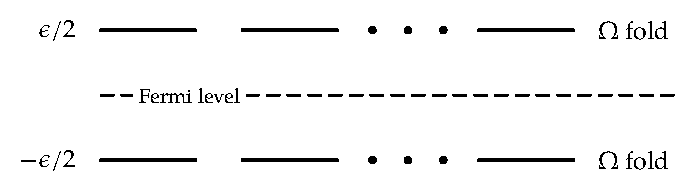
\includegraphics[width=0.75\textwidth]{pictures/5_1}
\par\end{centering}
\caption{\label{fig:5_1}示意模型中的能级结构（两能级相距$\epsilon$，各具$\Omega$重简并，其间为费米面）。}
\end{figure}

然而必须强调的是，算符$K_{0},K_{\pm}$与坐标空间中的转动毫无关系，它们通常被称为准自旋（quasi-spin）算符。为了应用Hartree-Fock方法，我们需要构建一般的Slater行列式$|\Phi\rangle$。Hamilton量\ref{eq:5.45}在费米面下方$\Omega$个能级与费米面上方相应能级之间的置换下保持不变。因此，在下文中我们局限于对这种置换完全对称的解。在这种情况下，仅存在一种激发粒子-空穴对的可能，最一般的Slater行列式$|\Phi\rangle$由复数$z$表征：

\begin{equation}
|\Phi\rangle=\mathcal{N}\exp\left(zK_{+}\right)|\Phi_{0}\rangle=\prod^{\Omega}_{m=1}a^{\dagger}_{0m}|-\rangle\label{eq:5.48}
\end{equation}
其中

\begin{equation}
|\Phi_{0}\rangle=\prod^{\Omega}_{m=1}c^{\dagger}_{-1m}|-\rangle\label{eq:5.49}
\end{equation}
且

\begin{align}
a^{\dagger}_{0m} & =D_{-0}c^{\dagger}_{-1m}+D_{+0}c^{\dagger}_{1m}\label{eq:5.50a}\\
a^{\dagger}_{1m} & =D_{-1}c^{\dagger}_{-1m}+D_{+1}c^{\dagger}_{1m}\label{eq:5.50b}
\end{align}
这里我们将新的上下能级分别记为0和1。借助式\ref{eq:5.50a}与\ref{eq:5.50b}，我们可以用新算符$a_{0m},a_{1m}$表示Hamilton量\ref{eq:5.45}。随后，在$D$归一化条件（$|D_{-0}|^{2}+|D_{+0}|^{2}=1$）下对$\langle\Phi|H|\Phi\rangle$关于$D_{\pm0}$变分，即可导出Lipkin模型中的Hartree-Fock方程：

\begin{equation}
\begin{pmatrix}-\frac{1}{2}\epsilon & -Q\\
-Q^{*} & \frac{1}{2}\epsilon
\end{pmatrix}\begin{pmatrix}D_{-0}\\
D_{+0}
\end{pmatrix}=\epsilon_{0}\begin{pmatrix}D_{-0}\\
D_{+0}
\end{pmatrix}\label{eq:5.51}
\end{equation}
其中

\begin{equation}
\chi=\frac{V(\Omega-1)}{\epsilon},\quad Q=\chi\epsilon D_{+0}D^{*}_{-0}
\end{equation}
这是通常的非线性方程，可通过迭代法求解。新的单粒子能量由下式给出：

\begin{equation}
\epsilon_{0,1}=\mp\frac{1}{2}\epsilon\sqrt{1+\left(\frac{2|Q|}{\epsilon}\right)^{2}}=\mp\frac{1}{2}\epsilon\sqrt{1+\chi^{2}\sin^{2}2\alpha}\label{eq:5.52}
\end{equation}
其中我们令$D_{-0}=\cos\alpha$，$D_{+0}=\sin\alpha\,\mathrm{e}^{-\mathrm{i}\varphi}$。由式\ref{eq:5.51}解出$D_{-0},D_{+0}$并代入$Q$的表达式，在$Q\neq0$的情形下，利用式\ref{eq:5.52}可得关于“形变”势$Q$的如下方程：

\begin{equation}
1=\frac{\chi}{\sqrt{1+\left(\frac{2|Q|}{\epsilon}\right)^{2}}}\label{eq:5.53}
\end{equation}
该方程仅在$\chi\ge1$时具有实数解，对应于下文给出的形变HF解。（式\ref{eq:5.53}与BCS理论的能隙方程极其相似，这绝非偶然，我们在第11.2节与附录F.5中将对此进行更为详尽的讨论。）

在坐标$\alpha,\varphi$下，基态能量表示为

\begin{equation}
E_{\mathrm{HF}}=-\frac{1}{2}\epsilon\Omega\left(\cos2\alpha+\frac{1}{2}\chi\sin^{2}2\alpha\cos2\varphi\right)\label{eq:5.54}
\end{equation}
自洽条件由能量对参数的极值给出：

\begin{align}
\frac{\partial E_{\mathrm{HF}}}{\partial\alpha} & =0=\epsilon\Omega\sin2\alpha\left(1-\chi\cos2\alpha\cos2\varphi\right)\label{eq:5.55}\\
\frac{\partial E_{\mathrm{HF}}}{\partial\varphi} & =0=\frac{1}{2}\epsilon\Omega\chi\sin^{2}2\alpha\sin2\varphi\nonumber 
\end{align}
从式\ref{eq:5.55}可以看出，根据$\chi$大于还是小于1，必须区分两种情况。在后一种情形（$\chi<1$）下，仅有一个解：

\begin{equation}
\varphi_{\mathrm{HF}}=0,\quad\alpha_{\mathrm{HF}}=0\quad(\chi<1)\label{eq:5.56}
\end{equation}
对于$\chi>1$，存在第二个解：

\begin{equation}
\varphi_{\mathrm{HF}}=0,\quad\chi\cos2\alpha_{\mathrm{HF}}=1\quad(\chi>1)\label{eq:5.57}
\end{equation}
可以证明该解对应能量的极小值，而第一个解变为极大值。这可以从该点处能量曲面的曲率看出：

\begin{equation}
\left.\frac{\partial^{2}E_{\mathrm{HF}}}{\partial\alpha^{2}}\right|_{\alpha_{\mathrm{HF}}}=2\epsilon\Omega\left(\chi-\frac{1}{\chi}\right)>0\quad(\chi>1)\label{eq:5.58}
\end{equation}
在\ref{fig:5_2}中，我们给出了$\chi\lessgtr1$时二维能量曲面（式\ref{eq:5.54}）沿$\varphi=0$的剖面线。

\begin{figure}[H]
\begin{centering}
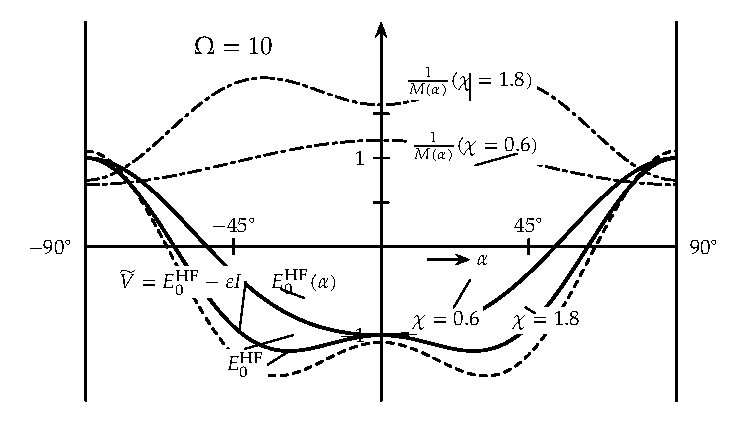
\includegraphics[width=0.75\textwidth]{pictures/5_2}
\par\end{centering}
\caption{\label{fig:5_2}$\chi\lessgtr1$时$E_{\mathrm{HF}}$作为$\alpha$的函数（实线）。其他四条曲线对应于生成坐标法（GCM，见第10.7.5小节）计算的量（引自\cite{Ho73}）。}
\end{figure}

从临界相互作用强度

\begin{equation}
\chi_{c}=\frac{V_{c}(\Omega-1)}{\epsilon}=1\label{eq:5.59}
\end{equation}
开始，位于$\alpha=0,\varphi=0$处的球形解变得不稳定，此时必须采用新的单粒子基底。在\ref{fig:5_3}中，展示了$\chi=6$时方程\ref{eq:5.51}的迭代求解过程。若从初值$\alpha_{1}=80^{\circ},\varphi_{1}=30^{\circ}$出发，后续各步依次为（\ref{fig:5_3}中的实线）：$\alpha_{2}=32.01^{\circ},\varphi_{2}=-30^{\circ}$；$\alpha_{3}=39.75^{\circ},\varphi_{3}=30^{\circ}$；$\alpha_{4}=40.19^{\circ},\varphi_{4}=-30^{\circ}$；……关于变量$\alpha$，解迅速收敛到$\alpha_{\mathrm{HF}}=40.20^{\circ}$（式\ref{eq:5.57}）；但关于变量$\varphi$，迭代解并未收敛，而是在$+30^{\circ}$与$-30^{\circ}$之间来回振荡。然而若改用梯度法（虚线），则可平滑收敛到真正极小解$\alpha_{\mathrm{HF}}=40.20^{\circ},\varphi_{\mathrm{HF}}=0^{\circ}$。在实际微观计算中，有时也会遇到类似情况：在某些自由度上解会来回振荡。

\begin{figure}[H]
\begin{centering}
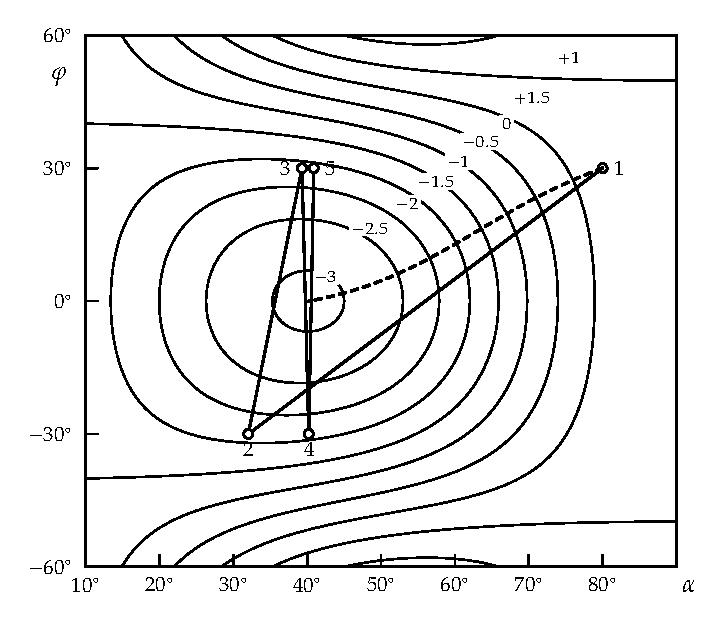
\includegraphics[width=0.75\textwidth]{pictures/5_3}
\par\end{centering}
\caption{\label{fig:5_3}通过迭代对角化（实线）与梯度法（虚线）求解HF方程的数值比较。}
\end{figure}


\section{Hartree-Fock方法与对称性\label{sec:Hartree-Fock=0065B9=006CD5=004E0E=005BF9=0079F0=006027}}

HF方程是非线性的，这意味这自洽势$\Gamma$不仅依赖于Hamilton量，也依赖于解（由密度矩阵$\rho$表示）。因此，这个势和Hamilton量不具有相同的对称性。我们由此可以说这个解的对称性破缺了。平移不变性的破缺我们已经遇到过，不过除此之外还有转动对称性和粒子数对称性（见\ref{chap:=005BF9=005173=008054=004E0E=008D85=006D41=006838}和\ref{chap:=0063A8=005E7F=007684=005355=007C92=005B50=006A21=00578B=00FF08HFB=007406=008BBA=00FF09}）通常人们会把从对称性保持到破缺的过程称为相变。这种对称性破缺的最大有点就是允许我们在简单的单粒子图像下去近似地考虑多体关联。更为细致的讨论将会在\ref{chap:=0063A8=005E7F=007684=005355=007C92=005B50=006A21=00578B=00FF08HFB=007406=008BBA=00FF09}，\ref{chap:=005BF9=0079F0=006027=007684=006062=00590D}和\ref{chap:=0076F4=0079EF=006CE2=0051FD=006570=0076F8=005173=007684=005B9A=007406}中给出，我们这里仅仅做如下论述：假设我们由一个Slater行列式$|\Phi\rangle$，它由形变的单粒子基$\{a^{\dagger}_{k}\}$组成。我们可以通过线性变换用球形基把它表示出来：
\[
a^{\dagger}_{k}=\sum_{q}D_{qk}c^{\dagger}_{q}
\]

我们因此得到了一系列球形基下占据数不同的Slater行列式之和：
\[
a^{\dagger}_{i_{1}}\dots a^{\dagger}_{i_{N}}|-\rangle=\sum_{q_{1}\dots q_{N}}d^{i_{1}\dots i_{N}}_{q_{1}\dots q_{N}}c^{\dagger}_{q_{1}}\dots c^{\dagger}_{q_{N}}|-\rangle
\]

这里系数$d^{i_{1}\dots i_{N}}_{q_{1}\dots q_{N}}$是一系列矩阵$D_{qk}$的乘积。当然，这种符号实际上对应着更一般的拟设，它包含了精确解，当然它绝对不是能用HF波函数描述的
\begin{comment}
原文经典不说人话，我这里翻译的已经尽量是人话了。这里实际上想说这个符号是个张量的符号，这种张量一般不能写成矩阵的张量积。如果这里真的是个一般的张量的话，这种形式的波函数应该可以张成整个空间，所以一定包含精确解。但是这个精确解一般来说写不成HF波函数的形式。
\end{comment}
。不论如何，我们可以看出一组基下的Slater行列式在另一组基下可能十分复杂，是一系列Slater行列式的叠加态。

当然，精确的波函数应当由Hamilton量的对称性，对称性的破缺只是因为我们想尽可能的维持独立粒子的图像。尽管如此，我们之后会尝试恢复破缺掉的对称性。我们将在\ref{chap:=005BF9=0079F0=006027=007684=006062=00590D}讨论这一点。然而，HF理论确实保留了特定的对称性，也就是所谓的自洽对称性。它们依赖于初始的密度$\rho^{(0)}$，以及HF场$\Gamma$：
\begin{equation}
S\Gamma[\rho]S^{\dagger}=\Gamma[S\rho S^{\dagger}]\label{eq:self-consistence sysmmetry}
\end{equation}

\begin{booknote*}
定理：如果 $S$ 是一个对称算符（酉算符或反酉算符），且与Hamilton量对易，那么有 $Sh[\rho]S^{-1}=h[S\rho S^{-1}]$。

证明（酉算符情景）：我们假设算符 $S$ 作用到产生算符上有：

\[
Sa^{\dagger}_{i}S^{-1}=\sum_{ii^{\prime}}S_{ii^{\prime}}a^{\dagger}_{i^{\prime}}
\]

则其作用到湮灭算符上有：

\[
Sa_{i}S^{-1}=\sum_{ii^{\prime}}S^{*}_{ii^{\prime}}a_{i^{\prime}}
\]

我们记其作用到态 $|i\rangle$ 后使其变为 $|\bar{i}\rangle$，根据上面的假设，我们可以把它用原来的基展开，得到：

\[
S|i\rangle=|\bar{i}\rangle=\sum_{i^{\prime}}S_{ii^{\prime}}|i^{\prime}\rangle
\]

单粒子密度矩阵为 $\rho_{ij}=\mathop{\text{Tr}}(\rho a^{\dagger}_{j}a_{i})$，对其做对称操作后记为$\bar{\rho}_{ij}$，即得到：

\[
\begin{aligned}\bar{\rho}_{ij} & =\mathop{\text{Tr}}(S\rho a^{\dagger}_{j}a_{i}S^{-1})\\
 & =\mathop{\text{Tr}}(\rho Sa^{\dagger}_{j}S^{-1}Sa_{i}S^{-1})\\
 & =\sum_{i^{\prime}j^{\prime}}S^{*}_{ii^{\prime}}S_{jj^{\prime}}\mathop{\text{Tr}}(\rho a^{\dagger}_{j^{\prime}}a_{i^{\prime}})\\
 & =\sum_{i^{\prime}j^{\prime}}S^{*}_{ii^{\prime}}S_{jj^{\prime}}\rho_{i^{\prime}j^{\prime}}
\end{aligned}
\]

对 HF Hamilton量做对称操作，即得到：

\[
\begin{aligned}\langle\bar{k}|h|\bar{l}\rangle & =\langle\bar{k}|t|\bar{l}\rangle+\sum_{ij}\langle\bar{k}i|V|\bar{l}j\rangle\rho_{ij}\\
 & =\langle\bar{k}|t|\bar{l}\rangle+\sum_{ij}\sum_{i^{\prime}j^{\prime}}S_{i^{\prime}i}S^{*}_{j^{\prime}j}\langle\bar{k}\bar{i^{\prime}}|V|\bar{l}\bar{j^{\prime}}\rangle\rho_{ij}\\
 & =\langle\bar{k}|t|\bar{l}\rangle+\sum_{ij}\langle\bar{k}\bar{i}|V|\bar{l}\bar{j}\rangle\bar{\rho}_{ij}\\
 & =\langle k|t|l\rangle+\sum_{ij}\langle ki|V|lj\rangle\bar{\rho}_{ij}
\end{aligned}
\]

证毕。这里要用到$\rho_{ij}=\rho_{ji}$。

推论：如果$S$保持单粒子密度矩阵不变，那么其与HFHamilton量$h$对易。（$S$保持单粒子密度矩阵不变等价于$\sum_{i^{\prime}j^{\prime}}S^{*}_{ii^{\prime}}S_{jj^{\prime}}\rho_{i^{\prime}j^{\prime}}=\rho_{ij}$，在零温下这等价于保持占据态不变。）

证明：

由于$S\rho S^{-1}=\rho$，由此$Sh[\rho]S^{-1}=h[S\rho S^{-1}]=h[\rho]$。即$S$与$h$对易。

推论：如果$\rho$在迭代中初始保持了一定的对称性，那么其之后一直保持这种对称性。

满足这一性质的有：偶偶核中的时间反演算符，宇称算符，忽略库伦相互作用时$N=Z$核中的同位旋交换算符，闭壳核（球对称）中的角动量算符，轴对称核中的对称轴方向角动量算符，忽略自旋轨道耦合项时的自旋算符。
\end{booknote*}
这意味着如果初始密度$\rho^{(0)}$具有特定的Hamilton量具有的对称性$S$，那么第一步得到的自洽场$h[\rho^{(0)}]$也如此。而下一步的密度$\rho^{(1)}$是通过对$h[\rho^{(0)}]$
\begin{comment}
原文$h[\rho^{(1)}]$
\end{comment}
对角化得到的，由此它必须具有相同的对称性。由此，在每一步迭代中，对称性$S$都被保留了。

自洽对称性的存在对实际的计算有以下影响\cite{Ri68}：
\begin{enumerate}
\item 如果我们期待最终的解具有特定的对称性，我们可以让初始密度$\rho^{(0)}$具有这个对称性，因此计算只在具有该对称性的基上进行，计算量就减小了。
\item 如果我们从特定对称性出发，我们将只能得到具有对称性的解，即最小能量是在具有这种对称性的波函数上变分得到的。例如，假如极小值是一个形变Slater行列式，但我们从一个球对称的密度矩阵出发，我们将永远也得不到这个解，尽管微小的数值误差可能让最终的解有微小的形变。
\item 如果我们有一个对称性$S$被破缺掉的解：
\[
S\rho S^{\dagger}=\rho_{1}\neq\rho
\]
那么从\ref{eq:self-consistence sysmmetry}可以得到变换后的密度对应的HFHamilton量$h[\rho_{1}]$：
\[
h[\rho_{1}]=S^{\dagger}h[\rho]S
\]
这意味着$\rho_{1}$也是HF方程的解：
\[
[h[\rho_{1}],\rho_{1}]=0
\]
在连续对称性的情况下，例如平移对称性和转动对称性，对一个对称性破缺的解，我们可以找到无数个简并的解。
\end{enumerate}
在下一节，我们将会看到密度依赖的两体相互作用在HF计算中的作用。在这种情况下，核力不一定再具有和裸核力一样的对称性。尽管如此，HF解在对称变换下的通常的性质依然会成立。只要我们要求相互作用满足一个非常宽松的性质：
\[
\hat{S}V[\rho]\hat{S}^{-1}=V[S\rho S^{-1}]
\]

以转动为例，这意味着一个转动过的系统中两体相互作用和用转动过的密度计算出来的相互作用相同。Skyrme力就满足这个条件。

\section{Hartree-Fock方法与密度依赖相互作用\label{sec:Hartree-Fock=0065B9=006CD5=004E0E=005BC6=005EA6=004F9D=008D56=0076F8=004E92=004F5C=007528}}

\subsection{有效相互作用方法\label{subsec:=006709=006548=0076F8=004E92=004F5C=007528=0065B9=006CD5}}

\subsubsection{Brückner-Hartree-Fock\label{subsubsec:Brueckner-Hartree-Fock}}

直接应用前面各节所述的Hartree-Fock方法的一个主要障碍在于，大多数裸核子-核子力都具有无穷大或者至少是非常强烈的排斥芯（参见第4章）。容易验证，对于硬芯势，进入Hartree-Fock势式(5.34)的两体矩阵元全都会发散到无穷大。解决这一困难的途径，是用第4.3.1节中讨论的Brückner$G$矩阵替换式(5.34)中的裸相互作用。事实上，这不仅因为解决了硬芯问题而带来便利，而且还可以证明，它是对整个多体问题中某些特定高阶项的自洽求和重整化（resummation）。由于我们此处手头尚未建立起完备的多体理论数学工具，我们将这一证明留到附录F.4中。

仿照式(5.38)，Brückner-Hartree-Fock（BHF）方程可写为（亦可参阅H. S. Köhler \cite{Ko75}以及W.
Wild \cite{Wi77}关于该主题的综述）：

\begin{equation}
\sum_{l'}\left\{ t_{ll'}+\sum^{A}_{i=1}\sum_{pp'}G^{\epsilon_{k}+\epsilon_{i}}_{lp',l'p}D_{pi}D^{*}_{p'i}\right\} D_{l'k}=\epsilon_{k}D_{lk}\label{eq:bhf_equation}
\end{equation}

这里$G$是由式(4.39)定义的Brückner$G$矩阵，是用某一特定单粒子势的基矢展开表示的。在作为式(5.72)之解的基矢中，相应的基态能量由下式给出：

\begin{align}
E^{\mathrm{BHF}}_{0} & =\sum^{A}_{i=1}t_{ii}+\frac{1}{2}\sum^{A}_{i,j=1}G^{\epsilon_{i}+\epsilon_{j}}_{ij,ij}\label{eq:bhf_e0_t}\\
 & =\sum^{A}_{i=1}\epsilon_{i}-\frac{1}{2}\sum^{A}_{i,j=1}G^{\epsilon_{i}+\epsilon_{j}}_{ij,ij}\label{eq:bhf_e0_eps}
\end{align}

对于基态能量而言，我们似乎只需要\ref{eq:bhf_equation}的空穴解。然而，\ref{eq:bhf_equation}的粒子解通过中间粒子能量$\epsilon_{n},\epsilon_{m}$进入到Bethe-Goldstone方程(4.39)中。因此，Brückner-Hartree-Fock解包含了一个复杂的双重自洽迭代过程。例如，可以通过如下迭代循环来求解：(i)
在初选的一组适宜基矢（例如简谐振子基）中通过式(4.39)计算$G$矩阵；(ii) 在该基矢下将\ref{eq:bhf_equation}对角化一次，得到一组新的基矢；(iii)
在这组新基矢下计算新的$G$矩阵；如此重复，直至达到自洽收敛。

然而，在这一迭代循环中，关于\ref{eq:bhf_equation}中$G$矩阵的能量依赖性会出现某种细微的歧义。由于我们事先并不知道最终的解，因此必须将$G^{\epsilon_{k}+\epsilon_{i}}_{lp',l'p}$的能量依赖性纳入迭代循环中。这样，在迭代的每一步中，我们必须取$\epsilon_{k}$为实际写出\ref{eq:bhf_equation}所在基矢对应的能量，即可以取$\epsilon_{k}$等于$\epsilon_{l}$或$\epsilon_{l'}$。对于$\epsilon_{i}$则不存在歧义，因为在迭代过程中$D_{pi}$被取为对角阵。对于BHF势能矩阵{[}参见式(5.34){]}，通常的约定取法是（参见例如\cite{Ba69a}；当然，最终的结果并不依赖于任何具体的约定）：

\begin{equation}
\Gamma^{\mathrm{BHF}}_{kk'}=\begin{cases}
\frac{1}{2}\sum^{A}_{i=1}\left(G^{\epsilon_{k}+\epsilon_{i}}_{ki,k'i}+G^{\epsilon_{k'}+\epsilon_{i}}_{ki,k'i}\right) & \text{当 }k,k'\leqslant\epsilon_{F},\\
\sum^{A}_{i=1}G^{\epsilon_{k}+\epsilon_{i}}_{ki,k'i} & \text{当 }k\leqslant\epsilon_{F},\,k'>\epsilon_{F},\\
\sum^{A}_{i=1}G^{\epsilon_{k'}+\epsilon_{i}}_{ki,k'i} & \text{当 }k'\leqslant\epsilon_{F},\,k>\epsilon_{F}.
\end{cases}\label{eq:bhf_gamma}
\end{equation}

$\Gamma^{\mathrm{BHF}}$的粒子-粒子矩阵元是一个略有争议的问题。对于给定的$G$矩阵，$\Gamma^{\mathrm{BHF}}$的粒子-粒子矩阵元并不直接影响\ref{eq:bhf_equation}的空穴解；然而，它们确实会影响粒子解，并进而通过双重自洽循环中的式(4.39)，间接地影响空穴解。我们可以证明（参见\cite{Ba69a,Ne70}中的讨论）：如果令$\Gamma^{\mathrm{BHF}}$的粒子-粒子矩阵元等于零，即

\begin{equation}
\Gamma^{\mathrm{BHF}}_{kk'}=0,\quad\text{当 }k,k'>\epsilon_{F},\label{eq:bhf_gamma_pp}
\end{equation}

那么原本在我们最初的\ref{eq:bhf_equation}和式(4.39)表述中所没有的三体关联就得到了有效的求和贡献。

\ref{eq:bhf_equation}不仅因为两体算符更加复杂而有别于通常的HF方程(5.38)，而且还因为$\Gamma^{\mathrm{BHF}}$现在依赖于我们想要计算的本征能量。因此，这是一个非线性问题，其中对应不同能量的解通常不再严格正交（但在球对称情况下，具有不同角动量的解依然是正交的）。然而，对于迭代求解而言，这并没有特别的妨碍\footnote{不过，人们仍然需要确保$\Gamma^{\mathrm{BHF}}$的能量依赖性不要过强，否则独立粒子图像可能不再成立。}。

正如我们在第4.3.1节所讨论的，$G$矩阵对核介质中的两粒子散射过程进行了求和。可以证明，\ref{eq:bhf_e0_eps}包含了此类过程对基态能量的全部贡献\cite{Ma67b}。在\ref{tab:bhf_results_reid}中，我们给出了以Reid软芯势(4.35)作为裸核力时，对$^{16}\mathrm{O}$、$^{40}\mathrm{Ca}$和$^{208}\mathrm{Pb}$进行Brückner-Hartree-Fock计算得到的方均根半径和单核子结合能。

\begin{table}[H]
\begin{centering}
\caption{\label{tab:bhf_results_reid}使用Reid软芯势的BHF计算结果与实验值的比较（来自\cite{DMS73}）}
\par\end{centering}
\centering{}%
\begin{tabular}{|c|c|c|c|}
\hline 
核素 & 物理量 & BHF & 实验值\tabularnewline
\hline 
\hline 
$^{16}\mathrm{O}$ & $-E_{0}/A\ (\mathrm{MeV})$ & 3.91 & 7.98\tabularnewline
 & $\mathrm{rms}\ (\mathrm{fm})$ & 2.50 & 2.73\tabularnewline
\hline 
$^{40}\mathrm{Ca}$ & $-E_{0}/A$ & 3.88 & 8.55\tabularnewline
 & $\mathrm{rms}$ & 3.04 & 3.48\tabularnewline
\hline 
$^{208}\mathrm{Pb}$ & $-E_{0}/A$ & 2.52 & 7.87\tabularnewline
 & $\mathrm{rms}$ & 4.51 & 5.50\tabularnewline
\hline 
\end{tabular}
\end{table}

\ref{tab:bhf_results_reid}中的结果是令人失望的。计算得到的结合能甚至还不到实验值的一半，而方均根半径也有约10\%–20\%的偏差。不过，结合能结果不佳并不十分令人意外，因为它是动能和势能这两个非常大的数值之间相抵消的差值。

然而，面对这一令人不满意的结果，人们必须考虑计入更复杂的过程\footnote{在此背景下，亦可参见超网链（hypernetted chain）形式体系\cite{PB73,FR75,FR76a,LS77,Ri79}。}。在多体阶层结构中，下一层便是三粒子散射项，其重要性应当依赖于系统的密度。正如我们在第4.3节中所看到的，表征两粒子关联力程的愈合距离（healing
distance）明显小于核子间的平均距离。因此，三个粒子同时处于愈合距离范围内的概率应当相当小。然而，这只是一个定性的论证\cite[p. 161]{Be71}。事实上，Kümmel及其合作者已经能够以完全自洽的方式将三体关联纳入基态能量的计算中（参见例如\cite{KLZ75,KLZ78}以及其中引用的文献）。他们还给出了强有力的论据，表明四体关联应当可以忽略。他们的结果非常引人注目，其与实验的符合程度得到了改善，尽管并不是非常剧烈。对于不同的核子-核子势，计算结果在$-E_{0}/A$与方均根半径平面上大致分布在一条光滑曲线上，如\ref{fig:bhf_coester_line}所示。这条曲线被称为Coester线（Coester
line）。Reid软芯势的结果大约位于该曲线最接近实验值的点上。鉴于文献\cite{KLZ75}中关于结果已经收敛的论断，剩余的差异必须归因于相对论效应或介子自由度。

\begin{figure}[H]
\begin{centering}
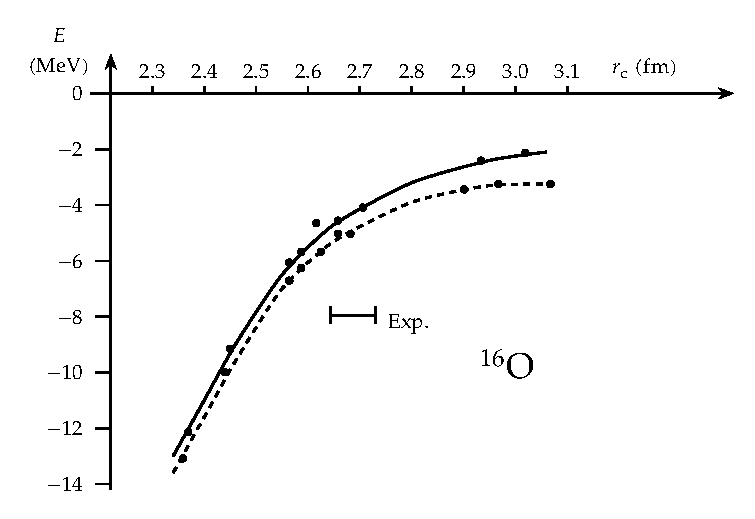
\includegraphics[width=0.75\linewidth]{pictures/5_4}
\par\end{centering}
\centering{}\caption{\label{fig:bhf_coester_line}不同核子-核子势的BHF计算结果（实线上的圆点）与包含三体关联的计算结果（虚线）以及实验值的比较（引自\cite{Wi77}）}
\end{figure}


\subsubsection{局域密度近似和变分原理\label{subsubsec:=005C40=0057DF=005BC6=005EA6=008FD1=004F3C=00548C=0053D8=005206=00539F=007406}}

在第4.3节中，我们看到硬芯势对两核子波函数的影响主要发生在其相对距离从0到约$1\,\mathrm{fm}$的范围内，也就是说，与大约$10\,\mathrm{fm}$的原子核半径相比，仅仅作用在非常短的距离上。这意味着Brückner$G$矩阵仅在相同的$r$值范围内才显著不同于裸相互作用$v(r)$。然而，一般而言，两核子相对坐标$r=|\boldsymbol{r}_{1}-\boldsymbol{r}_{2}|$约$1\,\mathrm{fm}$的变动，意味着质心坐标也有相近尺度的变化。核密度$\rho(\boldsymbol{R})=\rho(\frac{1}{2}(\boldsymbol{r}_{1}+\boldsymbol{r}_{2}))$在这样大小的$\boldsymbol{R}$范围内并不会发生很大改变（至少在核内部是如此）。因此，在每个$\rho(\boldsymbol{R})$值处计算核$G$矩阵时，假设原子核在$\boldsymbol{R}$附近的局域表现得就像是一块密度为$\rho(\boldsymbol{R})$的核物质\footnote{关于核物质理论，参见综述文献\cite{Be71,Sp72,JLM76}。}，这似乎是一个非常合理的假设。事实上，这种论证思路与Thomas-Fermi近似（参见第13章）非常接近。更明确地说，这意味着在利用\ref{eq:bhf_gamma_pp}写出的Bethe-Goldstone方程(4.39)中：

\begin{equation}
G^{W}=\bar{v}+\bar{v}\frac{Q_{F}}{W-Q_{F}\Gamma Q_{F}}G^{W}\label{eq:bg_gw}
\end{equation}

我们将投影算符$Q_{F}$替换为它在密度为$\rho(\boldsymbol{R})$的核物质中的表达式$Q^{\mathrm{NM}}_{F}$。由于$Q_{F}$式(4.41)可以由非局域单粒子密度$\rho(\boldsymbol{r},\boldsymbol{r}')=\sum^{A}_{i=1}\varphi_{i}(\boldsymbol{r})\varphi^{*}_{i}(\boldsymbol{r}')$表示为：

\begin{equation}
\langle\boldsymbol{r}_{1}\boldsymbol{r}_{2}|Q_{F}|\boldsymbol{r}'_{1}\boldsymbol{r}'_{2}\rangle=[\delta(\boldsymbol{r}_{1}-\boldsymbol{r}'_{1})-\rho(\boldsymbol{r}_{1},\boldsymbol{r}'_{1})][\delta(\boldsymbol{r}_{2}-\boldsymbol{r}'_{2})-\rho(\boldsymbol{r}_{2},\boldsymbol{r}'_{2})]\label{eq:qf_matrix_elem}
\end{equation}

这意味着在\ref{eq:qf_matrix_elem}中，$\rho$必须替换为其核物质中的取值{[}参见式(13.20){]}：

\begin{equation}
\rho^{\mathrm{NM}}(\boldsymbol{r},\boldsymbol{r}')=\frac{3}{k_{F}(\boldsymbol{R})s}j_{1}(k_{F}(\boldsymbol{R})s)\rho(\boldsymbol{R})\label{eq:rho_nm}
\end{equation}

其中$\boldsymbol{s}=\boldsymbol{r}-\boldsymbol{r}'$，$\boldsymbol{R}=\frac{1}{2}(\boldsymbol{r}+\boldsymbol{r}')$，$j_{1}$是球Bessel函数。\ref{eq:rho_nm}对$\boldsymbol{R}$的依赖性来源于我们仅在$\boldsymbol{R}$附近将原子核局域地当作核物质处理。$k_{F}$与$\rho$之间的关系一如既往地由下式给出{[}参见式(5.91)、式(13.22)和式(13.23){]}：

\begin{equation}
\rho(\boldsymbol{R})=\frac{2}{3\pi^{2}}k^{3}_{F}(\boldsymbol{R})\label{eq:rho_kf_rel}
\end{equation}

与有限核精确密度矩阵的数值比较表明\cite{Ne75}，在原子核内部，$\rho$的非局域行为能被\ref{eq:rho_nm}极其优良地近似，并且在整个核表面区域也得到了合理的再现。因此我们可以得出结论：此处所描述的对$G$矩阵的局域密度近似是相当成功的。

原则上，以此种方式计算的$G$矩阵依赖于三个变量：$\boldsymbol{r}=\boldsymbol{r}_{1}-\boldsymbol{r}_{2}$、$\boldsymbol{r}'=\boldsymbol{r}'_{1}-\boldsymbol{r}'_{2}$以及$\boldsymbol{R}=\frac{1}{2}(\boldsymbol{r}_{1}+\boldsymbol{r}_{2}-\boldsymbol{r}'_{1}-\boldsymbol{r}'_{2})$，即$G=G_{\boldsymbol{r},\boldsymbol{r}';\boldsymbol{R}}$。然而事实表明，$G$对总动量$\boldsymbol{P}$（与$\boldsymbol{R}$共轭的变量）的依赖性很弱，通常我们将其置为其平均值\cite{BGW58}：

\[
G_{\boldsymbol{r},\boldsymbol{r}';\boldsymbol{P}}\simeq G_{\boldsymbol{r},\boldsymbol{r}';\boldsymbol{P}_{\mathrm{av}}}
\]

Negele \cite{Ne70}进一步简化了$G$的表达式。他将式(5.73)的$G$矩阵中出现的起始能量$W=\epsilon_{i}+\epsilon_{j}$替换为一个平均值，该平均值取为核物质中平均空穴能量的两倍。通过这种方式，我们消除了式(5.72)中单粒子势对态的依赖性，相应的本征函数系构成了一组完备的正交归一基。下一步则是用一个有效局域算符$v^{\mathrm{eff}}(\boldsymbol{r})$来表示$G_{\boldsymbol{r},\boldsymbol{r}'}$（我们略去具体实现的细节，读者可参阅文献\cite{Ne70}\footnote{关于“局域”密度近似的其他应用，参见\cite{Ko65,NV70,CS72,NR72}。}）。此外，该有效相互作用经过唯象的重整化，以给出正确的核物质体积能项{[}参见Bethe-Weizsäcker公式(1.4){]}。从这个意义上说，Negele的“密度依赖HF”（DDHF）方法仍然是一种半唯象的方案。

Negele理论中还有一个至关重要的要素我们此前尚未提及：在\ref{tab:bhf_results_reid}中，我们看到纯粹的BHF计算并不能给出令人满意的结果；因此，必须寻求更好的方法。事实证明，将基态能量(5.73)中的$G$替换为局域密度近似，并像纯HF情况那样{[}式(5.29){]}对单粒子波函数进行能量变分，这一极具直观吸引力的构想带来了极好的计算结果。在这种情况下，Hartree-Fock
Hamilton量变为{[}参见式(5.32){]}：

\begin{equation}
h^{\mathrm{HF}}_{kk'}=\frac{\delta E[\rho]}{\delta\rho_{k'k}}=t_{kk'}+\sum_{qq'}\bar{v}^{\mathrm{eff}}_{kq'k'q}\rho_{qq'}+\left\langle \Phi\left|\frac{\delta v^{\mathrm{eff}}}{\delta\rho_{k'k}}\right|\Phi\right\rangle \label{eq:ddhf_h_var}
\end{equation}

其中$|\Phi\rangle$是与密度$\rho$对应的Slater行列式。对于密度无关的力，式(5.81)直接还原为通常的HF
Hamilton量。然而对于密度依赖的力，我们多出了一个附加项$\delta v^{\mathrm{eff}}/\delta\rho$，通常称之为重排势（rearrangement
potential）或饱和势（saturation potential）。它源自$v^{\mathrm{eff}}(\rho)$中的密度依赖性，并在实际数值计算中起着极其重要的作用。但必须强调的是，刚才所描述的变分方法并不等价于通过试探波函数变分来极小化原始多体Hamilton量(5.25)的期望值。这意味着，至少在原则上，由\ref{eq:ddhf_h_var}计算出的基态能量有可能低于真实的精确能量。该方法的合理性首先建立在其巨大的成功之上；在理论上，我们可以说附加项$\delta v^{\mathrm{eff}}/\delta\rho$在某种程度上计入了三体散射项\cite{Ne75}（在壳模型空间中，$\delta v^{\mathrm{eff}}/\delta\rho$具有六个指标）。在\ref{tab:ddhf_results}中，我们展示了使用DDHF方法相比于BHF所取得的显著改善\cite{Ne70,NV75}。

\begin{table}[H]
\begin{centering}
\caption{\label{tab:ddhf_results}密度依赖Hartree-Fock方法（DDHF）计算的结合能（以MeV为单位）与方均根半径（以fm为单位）}
\par\end{centering}
\centering{}%
\begin{tabular}{|c|c|c|c|c|}
\hline 
核素 & 物理量 & BHF & DDHF & 实验值\tabularnewline
\hline 
\hline 
$^{16}\mathrm{O}$ & $-E_{0}/A$ & 3.91 & 7.59 & 7.98\tabularnewline
 & $\mathrm{rms}$ & 2.50 & 2.75 & 2.73\tabularnewline
\hline 
$^{40}\mathrm{Ca}$ & $-E_{0}/A$ & 3.88 & 7.99 & 8.55\tabularnewline
 & $\mathrm{rms}$ & 3.04 & 3.46 & 3.48\tabularnewline
\hline 
$^{208}\mathrm{Pb}$ & $-E_{0}/A$ & 2.52 & 7.83 & 7.87\tabularnewline
 & $\mathrm{rms}$ & 4.51 & 5.49 & 5.50\tabularnewline
\hline 
\end{tabular}
\end{table}

求解DDHF方程是一项非常复杂的任务，因为交换项(5.43)意味着必须求解一个积分微分方程。然而，核力具有相当短的力程这一事实可以被用来简化问题，从而使得非局域交换项可以围绕其局域值按非局域程度进行展开。这种方法极其自然地为采用唯象Skyrme力的非常成功的HF方案提供了理论辩护，我们将在接下来研究这一方案\cite{Ne75}。

\subsection{Skyrme力的Hartree-Fock计算\label{subsec:Skyrme=00529B=007684Hartree-Fock=008BA1=007B97}}

\subsubsection{一般评述\label{subsubsec:=004E00=00822C=008BC4=008FF0}}

已经有许多不同的核力用于Hartree-Fock方法的计算。对这些核力给出一个综述超出了本书的范围（对于最近的综述，见\cite{QF78}）。他们中的许多——尤其是没有使用密度依赖项的核力——不能同时描述好结合能，半径，以及轻核和重核的正确的单粒子能谱（例如，\cite{Vo65,MB65,BB67,NDK68,PS68,SFW69,SP70}）。

Skyrme力作为一个唯象核力，很好的复现了整个元素周期表的结合能和半径\footnote{有一大批相似的唯象的密度依赖零程\cite{Mo70,LV71,La72,EM72,BJS75,Ko76,LB76,TK76,KKS77,SM78}或者有限程\cite{Kr70,ZR71,RPS72,LMV73,Go75b,RBP77}核力在HF计算中表现出了和Skyrme力相似的性质。}。同由局域密度近似得到的Negele力一样，Skyrme力是密度依赖的，不能在变分原理中简单的直接利用。形式上讲，这一困难可以通过把Skyrme力考虑成三体力来克服。

\subsubsection{利用Skyrme力计算能量\label{subsubsec:=005229=007528Skyrme=00529B=008BA1=007B97=0080FD=0091CF}}

我们从式(4.104)给出的Skyrme力出发，计算相应的Hamilton量在由单粒子波函数$\varphi_{i}(\boldsymbol{r},\sigma,q)$构成的Slater行列式$|\Phi\rangle$下的期望值。这里$\sigma=\pm\frac{1}{2}$是自旋量子数，$q=\pm\frac{1}{2}$是电荷量子数（质子或中子）。我们将波函数写为二分量旋量：

\begin{equation}
\varphi_{i}(\boldsymbol{r},\sigma,q)=\varphi_{i}(\boldsymbol{r},q)\chi_{\sigma_{i}}(\sigma)=\left(\begin{array}{c}
\varphi_{i}(\boldsymbol{r},q,\frac{1}{2})\\
\varphi_{i}(\boldsymbol{r},q,-\frac{1}{2})
\end{array}\right)\label{eq:skyrme_spinor}
\end{equation}

单粒子密度矩阵在坐标表象中具有如下形式{[}参见式(C.16){]}：

\begin{equation}
\rho(\boldsymbol{r}\sigma q,\boldsymbol{r}'\sigma'q')=\langle\Phi|a^{\dagger}_{\boldsymbol{r}'\sigma'q'}a_{\boldsymbol{r}\sigma q}|\Phi\rangle=\delta_{qq'}\rho_{q}(\boldsymbol{r}\sigma,\boldsymbol{r}'\sigma')\label{eq:density_matrix_coord}
\end{equation}

其中质子和中子的密度矩阵互不混合。总密度矩阵由下式给出：

\begin{equation}
\rho(\boldsymbol{r}\sigma,\boldsymbol{r}'\sigma')=\rho_{p}(\boldsymbol{r}\sigma,\boldsymbol{r}'\sigma')+\rho_{n}(\boldsymbol{r}\sigma,\boldsymbol{r}'\sigma')=\sum^{A}_{i=1}\varphi_{i}(\boldsymbol{r},\sigma,q_{i})\varphi^{*}_{i}(\boldsymbol{r}',\sigma',q_{i})\label{eq:total_density_matrix}
\end{equation}

为了计算结合能，我们需要如下局域密度量\cite{VB72}：

(i) 核子密度：

\begin{align}
\rho_{q}(\boldsymbol{r}) & =\sum_{\sigma}\rho_{q}(\boldsymbol{r}\sigma,\boldsymbol{r}\sigma)=\sum^{A}_{i=1}\delta_{q_{i}q}\sum_{\sigma}|\varphi_{i}(\boldsymbol{r},\sigma,q)|^{2}\label{eq:rho_q_def}\\
\rho(\boldsymbol{r}) & =\rho_{p}(\boldsymbol{r})+\rho_{n}(\boldsymbol{r})\label{eq:rho_tot_def}
\end{align}

(ii) 动能密度：

\begin{align}
\tau_{q}(\boldsymbol{r}) & =\sum_{\sigma}\left[\boldsymbol{\nabla}\cdot\boldsymbol{\nabla}'\rho_{q}(\boldsymbol{r}\sigma,\boldsymbol{r}'\sigma)\right]_{\boldsymbol{r}=\boldsymbol{r}'}=\sum^{A}_{i=1}\delta_{q_{i}q}\sum_{\sigma}|\boldsymbol{\nabla}\varphi_{i}(\boldsymbol{r},\sigma,q)|^{2}\label{eq:tau_q_def}\\
\tau(\boldsymbol{r}) & =\tau_{p}(\boldsymbol{r})+\tau_{n}(\boldsymbol{r})\label{eq:tau_tot_def}
\end{align}

(iii) 自旋-轨道（流）密度矢量：

\begin{align}
\boldsymbol{J}_{q}(\boldsymbol{r}) & =(-\mathrm{i})\sum_{\sigma\sigma'}\left[\boldsymbol{\nabla}\rho_{q}(\boldsymbol{r}\sigma,\boldsymbol{r}'\sigma')\times\langle\sigma|\boldsymbol{\sigma}|\sigma'\rangle\right]_{\boldsymbol{r}=\boldsymbol{r}'}\nonumber \\
 & =(-\mathrm{i})\sum^{A}_{i=1}\delta_{q_{i}q}\sum_{\sigma\sigma'}\varphi^{*}_{i}(\boldsymbol{r},\sigma',q)\left[\boldsymbol{\nabla}\varphi_{i}(\boldsymbol{r},\sigma,q)\times\langle\sigma'|\boldsymbol{\sigma}|\sigma\rangle\right]\label{eq:J_q_def}\\
\boldsymbol{J}(\boldsymbol{r}) & =\boldsymbol{J}_{p}(\boldsymbol{r})+\boldsymbol{J}_{n}(\boldsymbol{r})\label{eq:J_tot_def}
\end{align}

利用这些密度量，总能量期望值可以表示为一个能量密度的空间积分：

\begin{equation}
E=\langle\Phi|H|\Phi\rangle=\int\mathcal{H}(\boldsymbol{r})\,\mathrm{d}^{3}r\label{eq:skyrme_E_integral}
\end{equation}

由于Skyrme力的零程特性以及只保留到动量二阶项的动量依赖性，Hamilton能量密度泛函$\mathcal{H}(\boldsymbol{r})$完全是局域的。它由动能项、Skyrme相互作用能密度以及Coulomb能密度三部分构成：

\begin{equation}
\mathcal{H}(\boldsymbol{r})=\frac{\hbar^{2}}{2m}\tau(\boldsymbol{r})+\mathcal{H}_{\mathrm{Skyrme}}(\boldsymbol{r})+\mathcal{H}_{\mathrm{Coul}}(\boldsymbol{r})\label{eq:skyrme_H_density}
\end{equation}

对于时间反演不变的球对称或轴对称偶偶核系统，Skyrme相互作用能密度具有如下优美而紧凑的形式：

\begin{align}
\mathcal{H}_{\mathrm{Skyrme}}(\boldsymbol{r}) & =\frac{1}{2}t_{0}\left[\left(1+\frac{1}{2}x_{0}\right)\rho^{2}-\left(x_{0}+\frac{1}{2}\right)(\rho^{2}_{p}+\rho^{2}_{n})\right]\nonumber \\
 & \quad+\frac{1}{4}\left(t_{1}+t_{2}\right)\rho\tau+\frac{1}{8}\left(t_{2}-t_{1}\right)(\rho_{p}\tau_{p}+\rho_{n}\tau_{n})\nonumber \\
 & \quad+\frac{1}{16}\left(t_{2}-3t_{1}\right)\rho\nabla^{2}\rho+\frac{1}{32}\left(3t_{1}+t_{2}\right)(\rho_{p}\nabla^{2}\rho_{p}+\rho_{n}\nabla^{2}\rho_{n})\nonumber \\
 & \quad+\frac{1}{4}t_{3}\rho_{p}\rho_{n}\rho-\frac{1}{2}W_{0}\left[\rho\boldsymbol{\nabla}\cdot\boldsymbol{J}+\rho_{p}\boldsymbol{\nabla}\cdot\boldsymbol{J}_{p}+\rho_{n}\boldsymbol{\nabla}\cdot\boldsymbol{J}_{n}\right]\nonumber \\
 & \quad+\frac{1}{16}\left(t_{1}-t_{2}\right)\left[\boldsymbol{J}^{2}_{p}+\boldsymbol{J}^{2}_{n}\right]-\frac{1}{32}\left(t_{1}+t_{2}\right)\boldsymbol{J}^{2}\label{eq:H_skyrme_full}
\end{align}

在具有对称核物质密度（$\rho_{n}=\rho_{p}=\frac{1}{2}\rho$）的情况下，自旋-轨道密度相互抵消，\ref{eq:H_skyrme_full}显著简化为仅依赖于标量密度的形式：

\begin{align}
\mathcal{H}_{\mathrm{Skyrme}}(\boldsymbol{r}) & =\frac{3}{8}t_{0}\rho^{2}+\frac{1}{16}t_{3}\rho^{3}+\frac{1}{16}\left(3t_{1}+5t_{2}\right)\rho\tau\nonumber \\
 & \quad+\frac{1}{64}\left(9t_{1}-5t_{2}\right)(\boldsymbol{\nabla}\rho)^{2}\label{eq:H_skyrme_symm}
\end{align}

在导出\ref{eq:H_skyrme_full}时，式(4.104)中的三体力$v^{(3)}_{123}=t_{3}\delta(\boldsymbol{r}_{1}-\boldsymbol{r}_{2})\delta(\boldsymbol{r}_{2}-\boldsymbol{r}_{3})$贡献了正比于$\rho^{3}$的项。值得特别指出的是，对于任何Hartree-Fock
Slater行列式，纯接触三体力$v^{(3)}$的能量期望值严格等价于一个具有如下形式的密度依赖两体有效相互作用：

\begin{equation}
v^{(2)}_{\rho}(\boldsymbol{r}_{1},\boldsymbol{r}_{2})=\frac{1}{6}t_{3}(1+P_{\sigma})\delta(\boldsymbol{r}_{1}-\boldsymbol{r}_{2})\rho\left(\frac{\boldsymbol{r}_{1}+\boldsymbol{r}_{2}}{2}\right)\label{eq:skyrme_density_dep_2body}
\end{equation}

在第5.6.1节中我们看到，当使用密度依赖相互作用时，我们必须先计算能量，然后再对密度进行变分。在这个意义上，Skyrme三体接触力完全等价于两体相互作用式(5.88)。然而，这种等价性仅对具有时间反演对称性的偶偶核严格成立。

为了更深入地理解Skyrme能量密度泛函的物理意义，我们可以考察无限大均匀核物质的特例。在均匀核物质中，密度是恒定的（$\boldsymbol{\nabla}\rho=0$），动能密度由Fermi球积分给出：

\begin{equation}
\tau=\frac{3}{5}k^{2}_{F}\rho=\frac{3}{5}\left(\frac{3\pi^{2}}{2}\right)^{2/3}\rho^{5/3}\label{eq:tau_nuc_matter}
\end{equation}

此时，每个核子的结合能为：

\begin{equation}
\frac{E}{A}=\frac{\mathcal{H}}{\rho}=\frac{3}{5}\frac{\hbar^{2}}{2m}k^{2}_{F}+\frac{3}{8}t_{0}\rho+\frac{1}{16}t_{3}\rho^{2}+\frac{3}{80}\left(3t_{1}+5t_{2}\right)k^{2}_{F}\rho\label{eq:E_over_A_nuc_matter}
\end{equation}

将核子数密度与Fermi动量之间的标准关系代入：

\begin{equation}
\rho=\frac{2}{3\pi^{2}}k^{3}_{F}\label{eq:rho_kf}
\end{equation}

核物质在平衡饱和密度$\rho_{0}$（对应$k_{F0}\simeq1.35\,\mathrm{fm}^{-1}$）处满足饱和条件：即单核子结合能取极小值$E/A=-16.0\,\mathrm{MeV}$，且压强为零：

\begin{equation}
P=\rho^{2}\frac{\partial(E/A)}{\partial\rho}=0\label{eq:saturation_pressure_zero}
\end{equation}

此外，核物质不可压缩模量（incompressibility）定义为能量对密度的二阶导数：

\begin{equation}
K=9\left[\rho^{2}\frac{\partial^{2}(E/A)}{\partial\rho^{2}}\right]_{\rho=\rho_{0}}=k^{2}_{F}\left[\frac{\partial^{2}(E/A)}{\partial k^{2}_{F}}\right]_{k_{F}=k_{F0}}\label{eq:incompressibility_def}
\end{equation}

最后，Coulomb相互作用能包括直接项（Hartree项）和由Slater局域密度近似处理的交换项（Fock项）：

\begin{equation}
\mathcal{H}_{\mathrm{Coul}}(\boldsymbol{r})=\frac{1}{2}e^{2}\rho_{p}(\boldsymbol{r})\int\frac{\rho_{p}(\boldsymbol{r}')}{|\boldsymbol{r}-\boldsymbol{r}'|}\,\mathrm{d}^{3}r'-\frac{3}{4}e^{2}\left(\frac{3}{\pi}\right)^{1/3}\rho^{4/3}_{p}(\boldsymbol{r})\label{eq:H_coulomb}
\end{equation}

\ref{eq:H_coulomb}中的交换能项是局域密度近似下的标准结果\cite{Sl51a}，它极好地近似了有限核中的精确交换项，同时极大地简化了数值计算。

\subsubsection{密度依赖Hartree-Fock方程的导出\label{subsubsec:=005BC6=005EA6=004F9D=008D56Hartree-Fock=0065B9=007A0B=007684=005BFC=0051FA}}

根据第5.6.1节的构想，为了获得Hartree-Fock Hamilton量，我们必须对泛函$E=\int\mathcal{H}(\boldsymbol{r})\,\mathrm{d}^{3}r$在保持单粒子波函数正交归一约束$\int\varphi^{*}_{i}(\boldsymbol{r})\varphi_{j}(\boldsymbol{r})\,\mathrm{d}^{3}r=\delta_{ij}$的条件下进行变分：

\begin{equation}
\frac{\delta}{\delta\varphi^{*}_{i}}\left[E-\sum_{k}\epsilon_{k}\int\sum_{\sigma}|\varphi_{k}(\boldsymbol{r},\sigma)|^{2}\,\mathrm{d}^{3}r\right]=0\label{eq:skyrme_variation}
\end{equation}

能量泛函对单粒子波函数$\varphi^{*}_{i}$的泛函导数可通过对能量密度中出现的各种局域密度量利用链式法则求导求得：

\begin{equation}
\frac{\delta E}{\delta\varphi^{*}_{i}(\boldsymbol{r})}=\left[\frac{\delta\mathcal{H}}{\delta\rho_{q}}\frac{\partial\rho_{q}}{\partial\varphi^{*}_{i}}+\frac{\delta\mathcal{H}}{\delta\tau_{q}}\frac{\partial\tau_{q}}{\partial\varphi^{*}_{i}}+\frac{\delta\mathcal{H}}{\delta\boldsymbol{J}_{q}}\cdot\frac{\partial\boldsymbol{J}_{q}}{\partial\varphi^{*}_{i}}\right]\label{eq:functional_derivative_chain}
\end{equation}

利用分部积分法将作用在变分上的梯度算符转移，最终得到的自洽单粒子Hartree-Fock方程具有如下微分算符形式：

\begin{equation}
\left[-\boldsymbol{\nabla}\cdot\left(\frac{\hbar^{2}}{2m^{*}_{q}(\boldsymbol{r})}\boldsymbol{\nabla}\right)+U_{q}(\boldsymbol{r})+\boldsymbol{W}_{q}(\boldsymbol{r})\cdot\frac{1}{\mathrm{i}}(\boldsymbol{\nabla}\times\boldsymbol{\sigma})\right]\varphi_{i}(\boldsymbol{r},q)=\epsilon_{i}\varphi_{i}(\boldsymbol{r},q)\label{eq:skyrme_hf_pde}
\end{equation}

\ref{eq:skyrme_hf_pde}形式上与带有坐标依赖有效质量的单粒子Schrödinger方程完全相同。其中包含三个自洽势场：

(1) 坐标依赖的位置有效质量（effective mass）：

\begin{equation}
\frac{\hbar^{2}}{2m^{*}_{q}(\boldsymbol{r})}=\frac{\hbar^{2}}{2m}+\frac{1}{4}\left(t_{1}+t_{2}\right)\rho(\boldsymbol{r})+\frac{1}{8}\left(t_{2}-t_{1}\right)\rho_{q}(\boldsymbol{r})\label{eq:effective_mass_def}
\end{equation}

在核内部，有效质量比值通常在$m^{*}/m\simeq0.6\sim0.8$之间；而在原子核外部区域（$\rho\to0$），有效质量自然平滑地趋于裸核子质量$m$。

(2) 局域中心单粒子势：$U_{q}(\boldsymbol{r})$包含了由动能密度、两体与三体Skyrme接触项、重排贡献以及静电Coulomb项共同构成的丰富结构：

\begin{align}
U_{q}(\boldsymbol{r}) & =t_{0}\left[\left(1+\frac{1}{2}x_{0}\right)\rho-\left(x_{0}+\frac{1}{2}\right)\rho_{q}\right]\nonumber \\
 & \quad+\frac{1}{4}t_{3}\left(\rho^{2}-\rho^{2}_{q}\right)+\frac{1}{4}\left(t_{1}+t_{2}\right)\tau+\frac{1}{8}\left(t_{2}-t_{1}\right)\tau_{q}\nonumber \\
 & \quad+\frac{1}{16}\left(t_{2}-3t_{1}\right)\nabla^{2}\rho+\frac{1}{32}\left(3t_{1}+t_{2}\right)\nabla^{2}\rho_{q}\nonumber \\
 & \quad-\frac{1}{2}W_{0}\left(\boldsymbol{\nabla}\cdot\boldsymbol{J}+\boldsymbol{\nabla}\cdot\boldsymbol{J}_{q}\right)+\delta_{qp}V_{\mathrm{Coul}}(\boldsymbol{r})\label{eq:U_q_center_pot}
\end{align}

其中质子的局域Coulomb势为：

\begin{equation}
V_{\mathrm{Coul}}(\boldsymbol{r})=e^{2}\int\frac{\rho_{p}(\boldsymbol{r}')}{|\boldsymbol{r}-\boldsymbol{r}'|}\,\mathrm{d}^{3}r'-e^{2}\left(\frac{3}{\pi}\right)^{1/3}\rho^{1/3}_{p}(\boldsymbol{r})\label{eq:V_coul_direct_exchange}
\end{equation}

(3) 自旋-轨道单粒子势矢量场：由双体自旋-轨道耦合常数$W_{0}$与密度梯度确定：

\begin{equation}
\boldsymbol{W}_{q}(\boldsymbol{r})=\frac{1}{2}W_{0}\left(\boldsymbol{\nabla}\rho+\boldsymbol{\nabla}\rho_{q}\right)+\frac{1}{8}\left(t_{1}-t_{2}\right)\boldsymbol{J}_{q}-\frac{1}{16}\left(t_{1}+t_{2}\right)\boldsymbol{J}\label{eq:W_q_spin_orbit}
\end{equation}

对于球对称核，自旋-轨道相互作用项简化为众所周知的单粒子壳模型形式：

\begin{equation}
\boldsymbol{W}_{q}(\boldsymbol{r})\cdot\frac{1}{\mathrm{i}}(\boldsymbol{\nabla}\times\boldsymbol{\sigma})=\frac{1}{r}W_{q}(r)(\boldsymbol{l}\cdot\boldsymbol{\sigma})\label{eq:spin_orbit_spherical}
\end{equation}

其中势阱主要集中在核表面区域（因为$\mathrm{d}\rho/\mathrm{d}r$在核表面处具有尖锐峰值）。这完美地解释了自旋-轨道势主要为表面效应的物理本性。

\subsubsection{结果的讨论\label{subsubsec:=007ED3=00679C=007684=008BA8=008BBA}}

Vautherin与Brink \cite{VB72}最初针对球形满壳核（例如$^{16}\mathrm{O}$、$^{40}\mathrm{Ca}$、$^{48}\mathrm{Ca}$、$^{90}\mathrm{Zr}$与$^{208}\mathrm{Pb}$）求解了Skyrme-Hartree-Fock方程。求解过程通过在球坐标系下将径向波函数离散化并在坐标格点上进行迭代自洽求解。随后，Skyrme有效相互作用被推广到形变核\cite{FQ73}以及巨共振激发态的随机相位近似（RPA）计算中。

为了拟合Skyrme力的各个参数，通常利用核物质的饱和性质（结合能、饱和密度、对称能与不可压缩系数）以及若干代表性双满壳核的基态结合能和电荷半径。历史上出现过若干经典的参数组合，其中最著名的是Skyrme
II（SII）\cite{VB72}与Skyrme III（SIII）\cite{BFG75}。在表5.3中，我们将不同理论模型计算的结合能和电荷半径与实验值进行了系统对比。

\begin{table}[H]
\begin{centering}
\caption{\label{tab:hf_results_comparison}不同理论方案与微观相互作用计算的双满壳核单核子结合能（以MeV为单位）与电荷半径（以fm为单位）的比较}
\par\end{centering}
\centering{}%
\begin{tabular}{|c|c|c|c|c|c|c|}
\hline 
核素 & 物理量 & 实验值 & Negele \cite{Ne70} & Campi \& Sprung \cite{CS72} & Nemeth等 \cite{NMH73} & Skyrme III \cite{BFG75}\tabularnewline
\hline 
\hline 
$^{16}\mathrm{O}$ & $E$ & -7.98 & -6.75 & -7.68 & -7.98 & -7.96\tabularnewline
 & $r_{c}$ & 2.73 & 2.80 & 2.75 & 2.77 & 2.69\tabularnewline
\hline 
$^{40}\mathrm{Ca}$ & $E$ & -8.55 & -7.49 & -8.33 & -8.47 & -8.54\tabularnewline
 & $r_{c}$ & 3.49 & 3.49 & 3.49 & 3.40 & 3.48\tabularnewline
\hline 
$^{48}\mathrm{Ca}$ & $E$ & -8.67 & -7.48 & -8.40 & -8.55 & -8.71\tabularnewline
 & $r_{c}$ & 3.48 & 3.52 & 3.51 & 3.44 & 3.53\tabularnewline
\hline 
$^{90}\mathrm{Zr}$ & $E$ & -8.71 & -7.85 & -8.63 & -8.70 & -8.71\tabularnewline
 & $r_{c}$ & 4.23 & 4.25 & 4.27 & 4.13 & 4.32\tabularnewline
\hline 
$^{208}\mathrm{Pb}$ & $E$ & -7.87 & -7.53 & -7.87 & -7.87 & -7.87\tabularnewline
 & $r_{c}$ & 5.50 & 5.44 & 5.45 & 5.22 & 5.57\tabularnewline
\hline 
\end{tabular}
\end{table}

从\ref{tab:hf_results_comparison}中可以看出，密度依赖Hartree-Fock理论（无论是微观局域密度近似还是唯象Skyrme力）都以极高的精度重现了从轻核到重核的基态结合能和电荷半径，整体偏差通常在百分之一以内。

值得强调的是总结合能与单粒子能量之和之间的差异。在通常的密度无关两体相互作用下，由式(5.39)可知总能量等于：

\begin{equation}
E=\frac{1}{2}\sum^{A}_{i=1}\left(t_{ii}+\epsilon_{i}\right)\label{eq:E_sum_density_indep}
\end{equation}

然而对于Skyrme力，由于存在密度依赖的三体相互作用，总能量表达式变为：

\begin{equation}
E=\frac{1}{2}\sum^{A}_{i=1}\left(t_{ii}+\epsilon_{i}\right)-\frac{1}{8}t_{3}\int\rho_{p}\rho_{n}\rho\,\mathrm{d}^{3}r\label{eq:E_sum_skyrme_rearrangement}
\end{equation}

正如第5.6.1.2节中所讨论的，\ref{eq:E_sum_density_indep}和\ref{eq:E_sum_skyrme_rearrangement}中的最后一项被称为重排项。对于密度无关的力，该项为零，此时不可能同时准确重现一个原子核的结合能与单粒子能谱。密度依赖相互作用引入的重排效应对于协调核基态饱和与单粒子谱间隙起着决定性的关键作用。

人们还计算了电子散射的角分布，并发现与实验数据符合得很好。这表明理论计算给出了正确的电荷分布。例如在图5.5(a)中，我们展示了$^{208}\mathrm{Pb}$的电荷分布与通过电子散射确定的唯象曲线的对比。\ref{fig:skyrme2_pb208_results}(b)
给出了相应的质子和中子平均势$U_{p}$、$U_{n}$以及有效质量比值$m^{*}/m$。HF电荷密度在原子核内部并非完全平坦恒定，而是显示出起源于壳效应的起伏波动。这些起伏小于在唯象Woods-Saxon势中由壳模型电荷密度所得到的起伏，但仍然大于实验观测到的波纹。相应的自洽平均场也表现出对Woods-Saxon势形状的偏离。对于较轻的原子核，这种偏离更为显著。图5.5(b)还给出了表征Skyrme势非局域性的比值$m^{*}/m$。它由参数组合$3t_{1}+5t_{2}$决定{[}参见\ref{eq:effective_mass_def}{]}。对于Skyrme
II，其非局域性相当显著。

有效质量对单粒子能量$\epsilon_{i}$具有强烈的影响。如果我们假设$A$核与$A-1$核系统的单粒子波函数完全相同，即忽略能级$i$中的空穴对核芯造成的极化效应，那么能级之间的能量差为：

\begin{equation}
E(A)-E_{i}(A-1)=t_{ii}+\sum_{j\leqslant A}\bar{v}^{(2)}_{ij,ij}+\frac{1}{2}\sum_{jk\leqslant A}\bar{v}^{(3)}_{ijk,ijk}\label{eq:koopmans_skyrme}
\end{equation}

对右端的计算表明\cite{VB72}，\ref{eq:koopmans_skyrme}恰好就是单粒子能量$\epsilon_{i}$，即HF
Hamilton量的本征值。因此，在\ref{fig:single_particle_energies_lead}中，我们将铅同位素区域的实验单粒子能级与计算出的单粒子能量$\epsilon_{i}$进行了比较。理论计算基本上得到了正确的单粒子能级次序，尽管定量上不同的参数组展现出了相当不同的能谱。然而必须强调的是，我们并不能先验地期待完全的定量一致，因为尚未计入的核芯极化效应在此发挥着不容忽视的作用\cite{RW73}。

\begin{figure}[H]
\begin{centering}
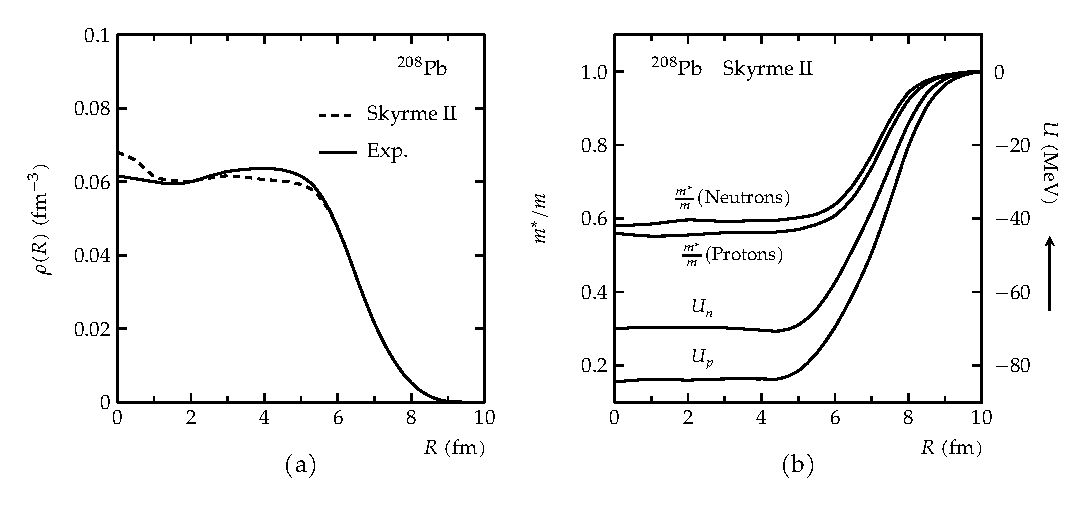
\includegraphics[width=0.85\linewidth]{pictures/5_5}
\par\end{centering}
\centering{}\caption{\label{fig:skyrme2_pb208_results}采用Skyrme II相互作用计算$^{208}\mathrm{Pb}$的Hartree-Fock结果。(a)
电荷分布；(b) 有效质量$m^{*}/m$与HF势$U(r)$（质子单粒子势未包含Coulomb项）（来自\cite{VB72}）}
\end{figure}

\begin{figure}[H]
\begin{centering}
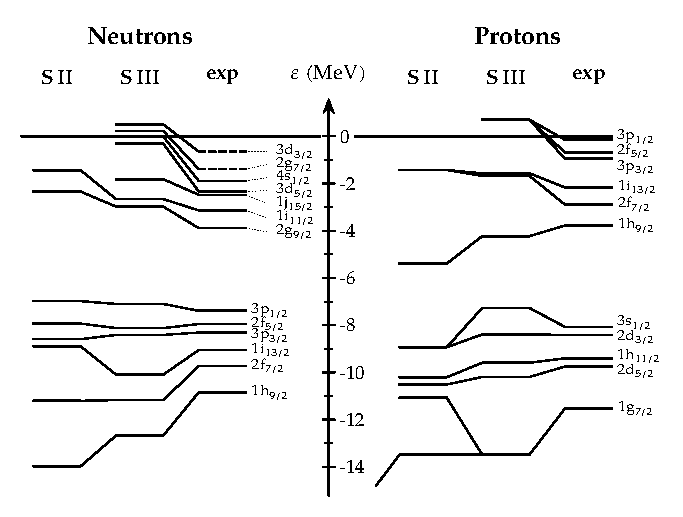
\includegraphics[width=0.8\linewidth]{pictures/5_6}
\par\end{centering}
\centering{}\caption{\label{fig:single_particle_energies_lead}铅核区实验与计算的单粒子能量。计算值由两种不同版本的Skyrme力获得。随着有效质量的增大，我们可以看到能谱的压缩（SII对应$m^{*}/m\simeq0.6$，SIII对应$\simeq0.75$）（来自\cite{BFG75}）}
\end{figure}


\section{结语\label{sec:=007ED3=008BED}}

总结本章的结果，我们可以说，第2章中所讨论的球形壳模型在此找到了微观理论基础。Hartree-Fock方法为从有效核子相互作用出发计算平均势提供了一个强有力的理论工具。为了获得与实验的定量符合，采用密度依赖的有效相互作用变得至关重要。在此框架下，我们能够非常优良地重现球形核的基态性质。在大多数情况下，计算出的单粒子能级展现出了正确的壳层排序；然而，在细节上它们与邻近奇质量核的实验单粒子激发谱之间仍存在一定偏离。

到目前为止，我们仅仅讨论了HF方法在闭壳核中的应用。事实上，只有在这些情况下，自洽平均场才能够保持球对称性。一旦在未填满的$j$壳层中放入一个或若干个粒子（开壳核HF
\cite{Ke63}），我们就必须决定原来简并的磁量子数$m$中哪一个应当被占据，从而导致轻微形变的密度分布（对于较大的$|m|$值，相对于量子化轴呈现扁椭球形变；对于较小的$|m|$值，则呈现长椭球形变）。这种形变密度在迭代的下一步中会产生形变的平均场，进而改变核芯中的单粒子波函数。通过这种方式，我们计入了由外加价粒子与其他核子相互作用所引起的关联效应。我们称这种效应为核芯的极化（polarization
of the core）。

只要我们只有单个或少数几个外加粒子，我们亦可以在球形基底中通过允许粒子-空穴（$ph$）激发的壳模型组态混合计算来处理这一相互作用。在这一图像中，价核子激发了核芯中的虚振动，我们通过粒子-振动耦合技术来处理极化效应（参见第9.3节）。

在许多实际应用中，人们往往通过将外加粒子以相等的概率$v^{2}_{m}=1/(2j+1)$均匀分布在下一个较高$j$壳层的所有$m$量子数上，从而仅以平均化的方式来考虑这种效应。在某种意义上，此时的波函数构成了一个具有球形密度分布的HFB态（参见第7章）。

原则上，只有在最高被占能级与最低未占能级之间存在明显的能隙时，平均场近似才具有充分的理论正当性。如果并非如此（例如次壳层闭合），便极易激发虚$ph$对，我们预期真实的波函数将比单一Slater行列式更加复杂{[}参见式(2.36){]}。基于这些理由，我们预期HF方法对幻数核的基态近似程度要远好于对那些偏离满壳组态若干粒子的核。这些开壳核在HF计算中表现出微小的形变，并在Fermi面附近具有许多几乎简并的能级。

如果我们继续向开壳层中添加粒子，形变就会变得越来越大。在远离满壳的开壳核中，我们会遇到强形变核（参见第3章）。在这里，HF极小值对应于一个具有显著形变的单一Slater行列式。由于平均势现在强烈地偏离球对称性，球形对称群的不可约表示（例如角动量$J$）不再是好量子数。波函数破坏了转动对称性。我们将在第3章和第11章中看到，这反映了体系自发对称性破缺（spontaneous
symmetry breaking）的物理机制。为了将计算出的形变态与真实的实验室系核态建立联系，必须通过恢复对称性（例如角动量投影）来恢复原本的转动不变性（参见第11章）。

在球形幻数核与强形变核之间，存在着一大类软核（soft nuclei）或过渡核（transitional nuclei）。在这些原子核中，势能面随形变的变化极为平缓，平均场近似无法给出清晰的能量极小值。此时，核体系呈现出剧烈的形变振荡和复杂的集体激发，必须借助生成坐标法（GCM，第10章）或玻色展开方法（第9章）等超越平均场的动力学方法进行处理。

形变Hartree-Fock理论在定量描述重质量稀土区和锕系核的转动带、内禀四极矩、六角形变以及裂变位垒方面取得了巨大成功。通过引入适当的外场下拉伸约束（constrained
HF），人们能够完整地绘制出核裂变位垒曲线\cite{FQ73,FQS73}。

总之，Hartree-Fock方法不仅构成了现代微观核结构理论的基石，而且为后续各章讨论的配对关联（BCS与HFB理论，第6、7章）、简谐微振动（RPA理论，第8章）、大振幅集体运动（GCM理论，第10章）以及对称性恢复（第11章）提供了最根本的自洽平均场出发点。



\chapter{对关联与超流核\label{chap:=005BF9=005173=008054=004E0E=008D85=006D41=006838}}

\section{简介和实验基础}

在第五章我们研究了描述核的基态的波函数。认为基态是直积波函数
\begin{comment}
Slater行列式。
\end{comment}
并且使能量最低，我们就得到了Hartree-Fock方法。正如我们所见，相关方程的解把一组单粒子基转换成了一组更好的单粒子基。变分原理等价于是说要求在基态和最低的激发态-单粒子空穴态之间的矩阵元为零。因此，正如我们在第四章所讨论的，Hartree-Fock方法部分地把相互作用的单粒子-空穴部分也就是说力的长程部分考虑了进去。在我们转而讨论关联导致的激发时，我们需要考虑导致了粒子粒子关联的力的短程部分（见第四章）。我们将会证明，可以通过形式上和单粒子空穴部分的力非常像的方法做到这一点，只需引入“准粒子”构成的广义的直积波函数。

当然我们通常必须同时考虑长程和短程关联，这是在下章的Hartree-Fock-Bogoliubov理论的框架下完成。我们姑且仅仅考虑纯粹的短程（粒子粒子或者对）关联，仅仅如此就能让我们理解Hartree-Fock图像最难以描述的效应。

现在我们总结一下与对关联相关的最重要的实验现象：
\begin{itemize}
\item 能隙。奇核和偶核在形变核的谱上有非常明显的区别。偶偶核只有少数可达$1.5\,\text{MeV}$的（集体）能级。它们可以被很好地描述为转动和振动能带。然而奇偶核非常不一样，它们在相同的能区有许多集体和单粒子态。\ref{fig:=00540C=004F4D=007D20=007684=0080FD=008C31}展示了一些锡同位素的能谱作为例子。
\end{itemize}
\begin{figure}[H]
\begin{centering}
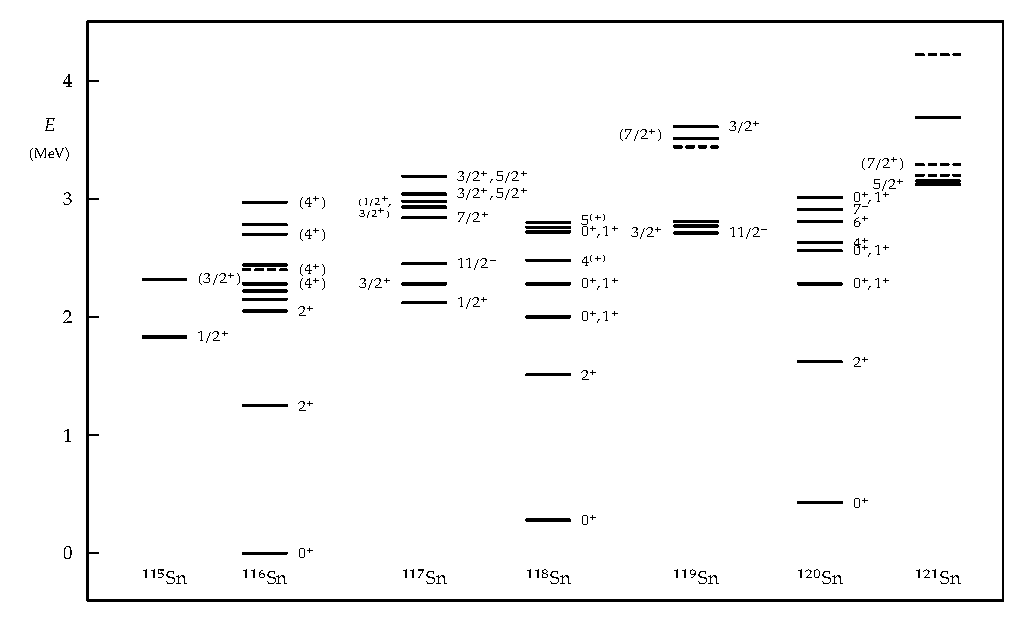
\includegraphics[width=0.65\linewidth]{pictures/6_1}
\par\end{centering}
\centering{}\caption{\label{fig:=00540C=004F4D=007D20=007684=0080FD=008C31}$\ce{_{50}Sn}$同位素的能谱}
\end{figure}

\begin{itemize}
\item 能级密度。如果我们假设在给定$j$下的壳中只有少量核子，由于角动量耦合有各种可能，而耦合得到的态能量都一样，因此是强简并的。单位能量态的数目可以很容易的估计，然而我们发现，在低激发能区域，我们估计的能级密度是实验值的接近两倍。
\item 奇偶效应。一个奇偶核的总结合能比相邻（算术意义上）的两个偶偶核的小。因此我们可以有关于临近核的质量的如下关系：
\[
M_{(A\text{ odd})}>\frac{M_{A-1}+M_{A+1}}{2}
\]

这被称为奇偶效应。
\item 形变原子核的惯性矩可以从旋转带的能级结构中测得。基于单粒子模型推导的结果和实验值差了一个两倍的因子。如果对效应被考虑近来，理论和实验可以很好的符合。
\item 形变。在壳模型里，如果我们对不同的核质量数计算核子密度分布，我们会发现，球对称形状的闭壳核逐渐变成了有大形变的半满壳核。核子数和闭壳核差距不大的核至少在基态的时候都是球形的。逐渐往壳层里填核子，会有一个区域，原子核有非常剧烈的形变，并且在半满的时候达到极大。
\item 低能$2^{+}$态。我们发现在偶数核
\begin{comment}
怀疑是偶偶核。
\end{comment}
里，在闭壳核附近，总是有一个角动量为$2$、宇称为正的能级。这些能级既不可以被解释为旋转能级，也不能被解释为单粒子激发能级。事实上，它们是振动的特征，这和对关联有很强的关系
\end{itemize}
为了理解所有这些现象，我们必须考虑核力短程部分引起的关联。正如在第二章提到的，偶偶核拥有自旋为零的基态，并且奇偶核的自旋可以由奇数核子的角动量确定。这些观察启示Go\"ppert
Mayer\cite{Ma50}做了一些初步的计算，计算显示，对于短程吸引的两体力来说，在一个给定$j$的壳层中，两个核子能量角度上讲更倾向于形成$I=0$的对而不是别的组合。如果忽略自旋，并且考虑$|lm\rangle$态和$|l,-m\rangle$的密度分布，这就可以很容易的理解，正如在\ref{fig:=007ED9=005B9A=0078C1=0091CF=005B50=006570=004E0B=007684=006838=005B50=005BC6=005EA6=005206=005E03}（或者是4.4.7中的讨论）中系统展示的那样。对于这些密度分布，很明显是在两个核子有着相同$|m|$的时候，它们密度的空间分布交叠达到最大。对于一个短程力来说，两个核子$\left|m\right|$相同但符号相反的时候能量是最低的
\begin{comment}
这似乎不是很容易精确证明？
\end{comment}
（它们方向相同的时候明显不符合Pauli不相容原理，在第三章中角动量
\begin{comment}
不知道是啥
\end{comment}
）。这里，符号相反意味着耦合后$I=0$。不考虑前面的系数，核子对的耦合成$I=0$，$M=0$角向部分为：

\begin{figure}[H]
\begin{centering}
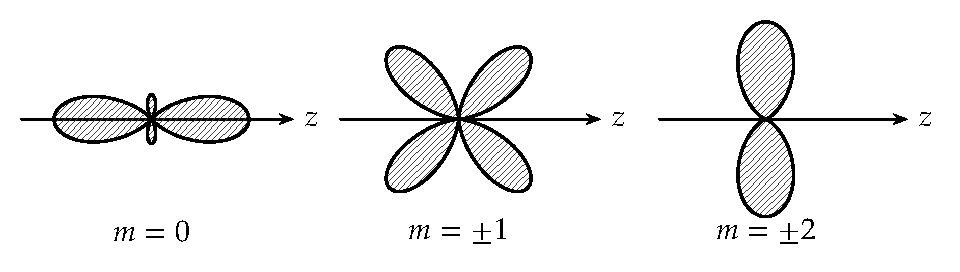
\includegraphics[width=0.6\linewidth]{pictures/6_2}
\par\end{centering}
\centering{}\caption{\label{fig:=007ED9=005B9A=0078C1=0091CF=005B50=006570=004E0B=007684=006838=005B50=005BC6=005EA6=005206=005E03}给定磁量子数下的核子密度分布}
\end{figure}

\begin{align}
\langle\theta_{1}\varphi_{1},\theta_{2}\varphi_{2}|nljjI=0,M=0\rangle & \propto\sum^{l}_{m=-l}(-1)^{m}Y_{lm}(\theta_{1},\varphi_{1})Y_{l,-m}(\theta_{2},\varphi_{2})\label{eq:angular part of pair}\\
 & =\frac{2l+1}{4\mathrm{\pi}}P_{l}(\cos\theta_{12})\nonumber 
\end{align}

这里$\theta_{12}$是两个核子的夹角。
\begin{comment}
这里有点没搞清楚是怎么来的。
\end{comment}
从上式可以看出，核子对的波函数只依赖于相对角度$\theta_{12}$。因此对于一个固定的$\theta_{12}$，核子对的波函数是一个核周围的均匀分布。由于两个核子的径向函数是相同的，通常不能得知关于核子对在空间中的位置更详细的信息，径向依赖性很大程度上是核子波函数的节点结构问题
\begin{comment}
这一句话是什么意思？
\end{comment}
。正如我们在\ref{fig:=009636Legendre=00591A=009879=005F0F=005173=004E8E=005939=0089D2=007684=0051FD=006570}中所看到的，$P_{l}(\cos\theta_{12})$在$\theta_{12}$处有一个宽度为$1/l$的峰。因此，两个核子有在角度上靠近的趋势。由于核力的短程性，这对于空间分布交叠取最大值是必须的。另一方面，因为不确定性原理的限制，两个核子也不能靠的太近。\footnote{可以非常简单的确定，如果$\psi(\boldsymbol{r}_{1},\boldsymbol{r}_{2})\sim\delta(\boldsymbol{r}_{1}-\boldsymbol{r}_{2})$，那么动量将会趋向于无穷大。}我们因此可以说，由于相互作用的短程性，两个核子想靠的尽可能的近，然而动能又想使核子分开，两者之间有一个妥协。

如果$j$壳层有不止一对核子， 泡利原理会稍微阻碍（$I=0$）电子对的形成，因为一些成对所需的$m$态已经被另一对核子占据。这种对的相互作用产生了某些特殊的性质，我们将在后面研究，但这并不破坏$j$壳层的处于的成对态的性质。此外，一些跃迁概率这样的典型性质与我们在给定的$j$壳层中拥有的对的数目成正比。如果我们考虑粒子和空穴之间的对称性，即既考虑粒子-粒子对也考虑空穴-空穴对，那么半满壳层是集体性最大的情况
\begin{comment}
这里集体性最大是什么意思？
\end{comment}
，而闭壳核则不可能形成对。
\begin{comment}
为什么？
\end{comment}

对于闭壳核之外的核，能量最低的态应当是所有核子都成对的态（除了奇偶核情况下的最后一个核子
\begin{comment}
奇奇核呢？
\end{comment}
）。为了激发偶偶核，我们必须打破一个对，然而对于奇偶核则只需要把单独的那个核子放到一个很低的能级上。由于对的结合能是$1-2\,\text{MeV}$，因此偶偶核和奇偶核第一激发态和基态的能量差就可以被定性的解释了。

其它上面提到的现象也可以利用对模型理解。由于偶偶核能谱底部能隙的存在，能级密度和实验符合的好多了，奇偶效应由此也非常显而易见。正如我们\ref{eq:angular part of pair}中看到的，$I=0$的对更倾向于球形（即没有方位偏好）。因此，由于对效应阻碍了形变，闭壳核附近的核也是球形的。而在远离闭壳核时则不是球形。事实上，更为精确的描述非常依赖于对力相对于长程（p-h）力的强度。尽管如此，从球形核到形变核的这一突变已经是可以理解的了。

与之紧密相关的还有开壳偶偶核能谱底部$2^{+}$态的存在。因为回复力，也即对效应和形变效应的差，非常小，闭壳核附近的球形核可以很容易激发出一个在它们平衡位形附近的形状振动。因此这些核会形变成一个椭球并且在球形附近以一个很低的频率振动（振动能级$2^{+}$）。

对相互作用的对角化并不能解释为像Hartree-Fock势那样的形式的平均静态能量的贡献。它是一种全新的效应，导致了所谓的对势。这一现象和金属中的超导现象类似。这就是Bohr，Mottelson和Pines\cite{BMP58}和Belyaev\cite{Be59}成功把Barden,
Cooper和Schrieffer{[}BCS 57{]}关于超导的理论应用于原子核的原因。

\section{辛弱数模型\label{sec:6.2_Seniority=0065B9=006848}}

正如我们在引言中说的，对关联是由于核子核子相互作用中的短程部分，并且这个相互作用对$I=0$的对最有效。在4.4.7节我们研究了一下这个问题；为了更进一步的研究对现象，我们考虑\ref{eq:pure pairing force}中的模型力，并考虑$N$个处在$2j+1$重简并的$j$壳的粒子，通过这个模型力相互作用。如果我们令$j$壳的能量为零，相应的
Hamilton 量应该具有这种形式\footnote{注意到接下来我们使用了BCS相位\ref{eq:BCS phases}。}：
\begin{equation}
H=-G\sum_{m,m^{\prime}>0}a^{\dagger}_{m^{\prime}}a^{\dagger}_{-m^{\prime}}a_{-m}a_{m}=-GS_{+}S_{-}\label{eq:Seniority Hamiltonian}
\end{equation}

这里：
\begin{equation}
S_{+}=\sum_{m>0}a^{\dagger}_{m}a^{\dagger}_{-m};\quad S_{-}=(S_{+})^{\dagger}\label{eq:quasi spin ladder operator}
\end{equation}

我们引入这两个算符，是因为它们可以被认为是假想的角动量的升降算符，我们称之为准自旋（就如同第五章中Lipkin模型中的情况）。它和真正的自旋没有任何关系，但是引入它对\ref{eq:Seniority Hamiltonian}的求解很有帮助\cite{Ke61}。同样是为了方便求解，我们继续对每个态$m(m>0)$都引入三个量：
\begin{align*}
s^{(m)}_{+} & =a^{\dagger}_{m}a^{\dagger}_{-m}\\
s^{(m)}_{-} & =a_{-m}a_{m}\\
s^{(m)}_{0} & =\frac{1}{2}(a^{\dagger}_{m}a_{m}+a^{\dagger}_{-m}a_{-m}-1)
\end{align*}

理由算符$a_{m}$和$a^{\dagger}_{m}$的对易关系，我们可以推导出相应的对易关系：
\begin{align*}
[s^{(m)}_{+},s^{(m)}_{-}] & =2s^{(m)}_{0}\\{}
[s^{(m)}_{0},s^{(m)}_{+}] & =s^{(m)}_{+}\\{}
[s^{(m)}_{0},s^{(m)}_{-}] & =-s^{(m)}_{-}
\end{align*}

因此我们发现$s^{(m)}_{+},s^{(m)}_{-},s^{(m)}_{0}$有着和角动量算符相同的对易关系。$s^{(m)}_{+}$和$s^{(m)}_{-}$是和$j_{+}$与$j_{-}$类比的升降算符。而$s^{(m)}_{0}$是和$j_{0}$类比的$z$方向的角动量算符。我们因此可以看出我们为什么称$\boldsymbol{s}^{(m)}$为$m$能级的准自旋算符了。

从$s^{(m)}_{0}$的定义中我们还可以发现它的本征值是$\pm\frac{1}{2}$，和$(m,-m)$是否是占据的有关。因此$\boldsymbol{s}^{(m)}$在$m$能级
\begin{comment}
原书为$j$-level。
\end{comment}
有零个或两个粒子的时候准自旋为$\frac{1}{2}$。如果只有一个粒子，那么$\boldsymbol{s}^{(m)}$的所有分量都为零，因此$\boldsymbol{s}^{(m)}$准自旋为零。

总准自旋算符$\boldsymbol{S}$定义为：
\begin{equation}
\boldsymbol{S}=\sum_{m>0}\boldsymbol{s}^{(m)}\label{eq:total quasi spin operator}
\end{equation}

这当然也是一个角动量算符，由此对 Hamilton 量\ref{eq:Seniority Hamiltonian}可以方便地写为：
\[
H=-G(\boldsymbol{S}\cdot\boldsymbol{S}-S^{2}_{0}+S_{0})
\]

我们又注意到：
\begin{equation}
S_{0}=\frac{1}{2}\sum_{m>0}(a^{\dagger}_{m}a_{m}+a^{\dagger}_{-m}a_{-m}-1)=\frac{1}{2}(\hat{N}-\Omega)\label{eq:S0}
\end{equation}

这里$\Omega=j+\frac{1}{2}$，是该壳层可能存在的对的数目
\begin{comment}
原书仅为“对的数目”。
\end{comment}
。因此$S_{0}$的本征值是整数或者半整数。进一步，根据角动量代数的性质我们可以得到：
\[
S\geq\left|S_{0}\right|=\frac{1}{2}\left|N-\Omega\right|
\]

根据\ref{eq:total quasi spin operator}，$S$的最大值是$S=\Omega/2$，因此我们可以看出$S$可以取$\Omega/2,\Omega/2-1,\Omega/2-2,\dots,\left|\Omega/2-N/2\right|$中的所有值。于是一个态可以用$S$和$S_{0}$标记，能量本征值因此为：
\[
E(S)=-G[S(S+1)-\frac{1}{4}(N-\Omega)^{2}+\frac{1}{2}(N-\Omega)]
\]

为了替代准自旋$S$，我们也可以引入一个量子数——辛弱数$s$\cite{Ra43}。它由下式给出：
\[
S=\frac{1}{2}(\Omega-s)
\]

这里：
\begin{align*}
s & =0,2,4,\dots,N\quad\text{如果}N\text{是偶数}\\
s & =1,3,5,\dots,N\quad\text{如果}N\text{是奇数}
\end{align*}

总能量关于辛弱数的关系可以如下给出：
\begin{align}
E(N,s) & =-\frac{G}{4}(N-s)(2\Omega-s-N+2)\nonumber \\
 & =-\frac{G}{4}(s^{2}-2s(\Omega+1)+2N(\Omega+1)-N^{2})\label{eq:E to seniority}
\end{align}

这一力的典型特点是能量的表达式中只有辛弱数量子数，而对其它所有量子数（除了$N$）都是简并的。此外，尽管能量的值强烈依赖于粒子数，谱并不如此。由于相邻能级的总准自旋差$1$，因此能量差为：
\begin{equation}
E(S-1)-E(S)=2GS\label{eq:energy difference to S}
\end{equation}

给定$N$，结合能随$S$增大而增加，因此基态就是所有的准自旋同向的情况，也就是说$S=\frac{1}{2}\Omega$或者$s=0$的情况。对于一个偶数粒子数的系统，第一个激发态的$s=2$，从\ref{eq:E to seniority}或\ref{eq:energy difference to S}我们可以得到：
\begin{equation}
E(N,s=2)-E(N,s=0)=G\Omega\label{eq:energy gap}
\end{equation}

因此激发能与$j$壳的粒子数无关。

如果我们在$j$壳只有两个粒子，辛弱数可以取$s=0,2$。两个全同核子可以耦合成$I=0,2,4,\dots,2j-1$。而只有$I=0$的态被影响了——它的能量被对相互作用降低了。其它的态都没有被影响，因此是简并的。因此我们看到基态（$s=0$）有$I=0$而激发态（$s=2$）有$I=2,4,6,\dots$，这意味着在基态，两个核子“成对”了，而在激发态发生了“拆对”。在\ref{fig:(a)=007EAF=005BF9=00529B=007684=004E24=007C92=005B50=008C31=003002(b)210Po=007684=0080FD=008C31}中展示了这一事实，同时为了比较，我们也展示了$\ce{^{210}Po}$（$1h9/2$壳中有两个中子）的低激发谱。一般的，基态结合能关于$N$的函数可以写成：
\begin{equation}
E(N,s=N)-E(N,s=0)=-E(N,s=0)=G\Omega\frac{N}{2}\left(1-\frac{N-2}{2\Omega}\right)\label{eq:E to N}
\end{equation}

\begin{figure}[H]
\begin{centering}
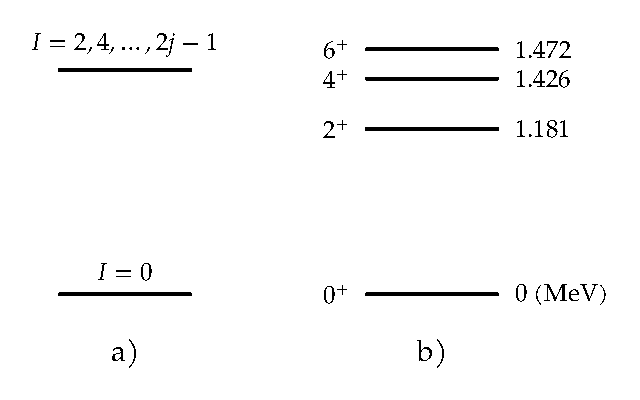
\includegraphics[width=0.65\linewidth]{pictures/6_3}
\par\end{centering}
\centering{}\caption{\label{fig:(a)=007EAF=005BF9=00529B=007684=004E24=007C92=005B50=008C31=003002(b)210Po=007684=0080FD=008C31}(a)纯对力的两粒子谱。(b)$\ce{^{210}Po}$（$1h9/2$壳中的2$p$）的能谱}
\end{figure}

可以看出，当粒子数远小于壳的简并度的时候，结合能随对的数目（$n=N/2$）是线性增长的，也就是说总能量就是一个对的结合能乘上对的数目。如果我们画出基态能量关于$n$的函数，我们将会得到一个谐振子谱\ref{fig:=005BF9=00632F=0052A8=007684=008C10=00632F=005B50=008C31}。这就是对振动谱，在诸如铅附近的区域被发现，我们将会在8.3.5广泛的讨论这一点。所有的\ref{fig:=005BF9=00632F=0052A8=007684=008C10=00632F=005B50=008C31}中的态都是准自旋最大的态（$s=0$），也就是基态，我们称之为$s=0$带。当然，这意味着也有$s=2$带等等。可以得到，两粒子在同一个带的不同态之间跃迁比在不同带间更容易
\begin{comment}
可能在后面有？
\end{comment}
。如果对的数目增加，由于Pauli不相容原理，$I=0$对的互相干扰会变得重要，因此谱\ref{eq:E to N}不再是谐振子的。

\begin{figure}[H]
\begin{centering}
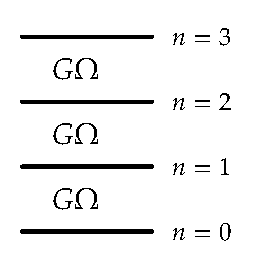
\includegraphics[width=0.4\linewidth]{pictures/6_4}
\par\end{centering}
\centering{}\caption{\label{fig:=005BF9=00632F=0052A8=007684=008C10=00632F=005B50=008C31}对振动的谐振子谱}
\end{figure}

我们可以看出，第一激发态的激发能和一个对的结合能相同，因此我们也可以说在第一激发态（$s=2$）两个核子拆对了。（不可能通过使对激发到能量更高的态上来得到第一激发态，因为我们的模型中只有一个能级。）推而广之，我们可以说辛弱数$s$的态有$s$个未成对的粒子（不论$s$是奇的还是偶的）。

显然，基态一定是非简并的，因为只有一种方式使得$\Omega$个$\frac{1}{2}$准自旋耦合成$S=\Omega/2$总准自旋。而要耦合出$s=2$的态却有$\Omega-1$种方式：
\[
t_{2}=\Omega-1=\begin{pmatrix}\Omega\\
1
\end{pmatrix}-\begin{pmatrix}\Omega\\
0
\end{pmatrix}
\]

考虑一个例子会更方便理解，例如$\Omega=4$。$s=2$的态可以表示为$\overset{1}{\rightarrow}\overset{2}{\rightarrow}\overset{3}{\rightarrow}\overset{a}{\leftarrow}$。有$4-1=3$种可能性把$a$和其它准自旋组合在一起，分别是$a1,a2,a3$。

可以确定，对任意偶数$s$，简并度可以由下式给出\cite{BS68a}：
\[
t_{s}=\begin{pmatrix}\Omega\\
s/2
\end{pmatrix}-\begin{pmatrix}\Omega\\
s/2-1
\end{pmatrix},\quad s\leq N
\]

辛弱数 Hamilton 量\ref{eq:Seniority Hamiltonian}对应的波函数也可以通过准自旋得到。对于$N=0$（空壳）和$N=2\Omega$（满壳），准自旋的第三分量分别全为$-\frac{1}{2}$或$\frac{1}{2}$。因此，真空态是$S=\frac{1}{2}\Omega,S_{0}=-\frac{1}{2}\Omega$的态：
\[
|\rangle=|\frac{1}{2}\Omega,-\frac{1}{2}\Omega\rangle
\]

满壳是$S=\frac{1}{2}\Omega,S_{0}=\frac{1}{2}\Omega$的态$|\Omega/2,\Omega/2\rangle$。如果我们用$|SS_{0}\rangle$表示任意一个准自旋态（这里$S_{0}=\frac{1}{2}(N-\Omega)$），不同偶数$N$的基态（$S=\Omega/2$）可以写为：
\begin{equation}
|\frac{1}{2}\Omega,S_{0}\rangle=|\frac{1}{2}\Omega,\frac{N-\Omega}{2}\rangle\propto S^{N/2}_{+}|\rangle\label{eq:ground state of seniority model}
\end{equation}

$S_{+}$的每次作用使得粒子数提高$2$。基态是$S^{2}$和$S_{0}$和$H$的本征态， 并且仅仅是$n=N/2$个对态的乘积。因此，我们可以说基态是对凝聚。

对于奇粒子系统，最后总有一个粒子无法成对，所以有一个准自旋必须为零。由此$S$可能的最大值将是$\frac{1}{2}(\Omega-1)$，基态为：
\[
|\frac{\Omega-1}{2},S_{0}\rangle\propto S^{\frac{1}{2}(N-1)}_{+}a^{\dagger}_{m}|\rangle
\]

由于$m$可以取$2\Omega$个不同的值$-j\leq m\leq j$，奇$N$粒子系统的基态因此是$2\Omega$简并的（与偶核的非简并相反）。这可以解释为什么奇核的基态附近能级密度很大，而偶核基态总是存在一个能隙。

正如我们已经看到的那样，辛弱数为2的态（$S=\frac{1}{2}\Omega-1$）是偶粒子的第一激发态。它们也可以用准自旋算符构建。

我们首先考虑$N=2$的情况，利用以下算符构建具有好的角动量量子数的态：
\[
A^{\dagger}_{IM}=\frac{1}{\sqrt{2}}\sum_{m_{1}m_{2}}C^{jjI}_{m_{1}m_{1}M}a^{\dagger}_{m_{1}}a^{\dagger}_{m_{2}}
\]

将其作用到真空态即可：
\begin{equation}
|IM\rangle=A^{\dagger}_{IM}|\rangle\label{eq:|IM>}
\end{equation}

由于$A^{\dagger}_{00}\propto S_{+}$（我们利用BCS相，\ref{eq:BCS phases}）,它们是准自旋算符的本征态，对$I=0$，有$S=\Omega/2$，对$I\neq0$，则有$S=\frac{1}{2}\Omega-1$。为了看出这一点，我们计算：
\[
S^{2}|IM\rangle=[S^{2},A^{\dagger}_{IM}]|\rangle+\frac{1}{2}\Omega\left(\frac{1}{2}\Omega+1\right)|IM\rangle
\]

右边第一项为：
\begin{align*}
[S^{2},A^{\dagger}_{IM}]|\rangle & =[S_{+}S_{-},A^{\dagger}_{IM}]|\rangle+[S^{2}_{0}-S_{0},A^{\dagger}_{IM}]|\rangle\\
 & =S_{+}[S_{-},A^{\dagger}_{IM}]|\rangle+[S^{2}_{0}-S_{0},A^{\dagger}_{IM}]|\rangle
\end{align*}

由于$S_{-}$正比于$A_{00}$，可以从Clebsch-Gordon系数的正交关系\cite{Ed57}中得到，对于$I\neq0$：
\[
[S_{-},A^{\dagger}_{IM}]|\rangle=0
\]

利用\ref{eq:S0}，我们最终得到对于$I\neq0$的情况来说：
\begin{align*}
S^{2}|IM\rangle & =-\Omega|IM\rangle+\frac{\Omega}{2}\left(\frac{\Omega}{2}+1\right)|IM\rangle\\
 & =\left(\frac{\Omega}{2}-1\right)\frac{\Omega}{2}|IM\rangle
\end{align*}

因此，两粒子态$|IM\rangle$在$I\neq0$的情况下是$S^{2}$的本征值为$S=\Omega/2-1$（或$s=2$）的本征态，也就是说，这两个粒子在$I\neq0$的情况下是不成对的。

由于算符$S_{+}$不改变$S$，只增加两个粒子，因此很容易构建偶$N$粒子系统（$N>2$）的第一激发态：
\[
|\frac{1}{2}\Omega-1,S_{0}\rangle\propto S^{\frac{1}{2}(N-2)}_{+}A^{\dagger}_{IM}|\rangle
\]

由于$S_{+}$是二阶球张量，因此这些$I\neq0$的态的角动量量子数为$I,M$，辛弱数为$2\text{。}$

当然，这些态是Hamilton 量\ref{eq:Seniority Hamiltonian}的本征能量为\ref{eq:E to seniority}的本征态。我们可以看出能量不依赖于$I,M$。正如我们之前说明的，更高的激发态是由未成对的粒子数标记的，也就是辛弱数$s$。这样的态可以通过算符$A^{\dagger}_{IM}$的相乘很容易的得到，但是样构造的态与低激发态的正交性，以及角动量守恒的特性并不显然。

许多情况下，我们并不需要精确构造波函数（例如，许多矩阵元可以通过角动量耦合的技巧得到。），这也是准自旋这套框架的优点。

举个例子，我们尝试计算四极算符的矩阵元：
\begin{align*}
Q_{20} & =\sum^{n}_{m=-j}q_{m}a^{\dagger}_{m}a_{m}=\sum_{m>0}q_{m}s^{(m)}_{0}\\
q_{m} & =\langle jm|r^{2}Y_{20}|jm\rangle
\end{align*}

由上式我们可以看出$Q_{20}$在准自旋空间是一个矢量
\begin{comment}
什么意思？
\end{comment}
。这一事实意味着四极算符的矩阵元关于对$S_{0}=\frac{1}{2}(N-\Omega)$的依赖（也就是对粒子数的依赖）可以由Wigner-Eckart定理\cite{Ed57}给出：
\[
\langle SS_{0}|Q_{20}|S^{\prime}S_{0}\rangle=(-)^{S-S_{0}}\begin{pmatrix}S & 1 & S^{\prime}\\
-S_{0} & 0 & S_{0}
\end{pmatrix}\langle S||Q_{2}||S^{\prime}\rangle
\]

由于四极跃迁是从辛弱数$s=0$的基态到$s=2$的激发态（由上式的选择定则给出），我们得到四极跃迁概率：
\begin{align*}
\left|\langle s=2|Q_{20}|s=0\rangle\right|^{2} & \propto\begin{pmatrix}\Omega/2 & 1 & \Omega/2-1\\
-S_{0} & 0 & S_{0}
\end{pmatrix}^{2}\propto\left(\frac{\Omega}{2}-S_{0}\right)\left(\frac{\Omega}{2}+S_{0}\right)=\frac{N}{2}\left(\Omega-\frac{N}{2}\right)
\end{align*}

从上式我们可以看出在引言中提到的跃迁概率的集体效应：它正比于核子对数$N/2$和空穴对数$(\Omega-N/2)$的乘积。因此，由于前面提到的基态的对的凝聚，集体效应在闭壳层的中间最为显著。实验上也发现闭壳层中间的核四极跃迁概率显著比壳模型计算的结果要高，我们与之符合的很好。

这一节我们提出的模型实际上非常简单，实际上情况当然要复杂的多。例如，我们必须考虑更多的能级和更现实的核力。尽管如此，我们想强调的是辛弱数模型的许多特点在更实际的情况下也是存在的，此外，这一模型在数学和物理上的简明性也比更为抽象的准粒子框架更好的反映了实际情况。准粒子框架正是我们下一节要介绍的，我们通常用它来处理更为复杂的情形。

\section{BCS模型}

\subsection{波函数}

辛弱数模型不紧急可以用在$j^{N}$组态。如果存在一些闭壳核芯上一些接近简并的$j$-壳，这一模型也可以推广\cite{Ta71,Ta76,LA74,Lo75}。然而，在远离闭壳核的情况下，原子核形变很大，能级也不再是均匀分布，辛弱数模型就完全失效了。

然而，辛弱数模型的结果告诉我们原子核中的对关联在开壳中是十分重要的，有理由相信远离闭壳核的时候这依然是正确的。接下来我们提出一个方法，这一方法既可以处理原子核中所有的核子，也可以简单的推广到不同类型的相互作用的情况。这一方法不能提供一个本征值问题的精确解，但是它像Hartree-Fock一样可以从变分原理得到。因此，对基态波函数做一个正确的拟设是很重要的。类比Bardeen，Cooper和Schrieffer\cite{BCS57}在超导问题中给出的基态，我们试着把偶偶核的基态表示成：
\begin{equation}
|\text{BCS}\rangle=\prod_{k>0}(u_{k}+v_{k}a^{\dagger}_{k}a^{\dagger}_{\bar{k}})|\rangle\label{eq:BCS wave function}
\end{equation}

这里$u_{k}$和$v_{k}$是变分参数。这里的乘积取遍了一半的组态空间，用$k>0$表示。对每一个大于零的$k$态，都有一个共轭态$\bar{k}<0$，并且$\{k,\bar{k}\}$生成了整个单粒子态空间。

$v^{2}_{k}$和$u^{2}_{k}$代表了一个对$(k,\bar{k})$占据或不占据的概率，它们是令能量期望值最小得到的。它们不是独立的，上述态归一化的要求给出：
\begin{equation}
|u_{k}|^{2}+|v_{k}|^{2}=1\label{eq:normalization of BCS}
\end{equation}

\begin{booknote*}
归一化使得：
\begin{align*}
\langle\text{BCS}|\text{BCS}\rangle & =\langle|\prod_{i>0}(u^{*}_{i}+v^{*}_{i}a_{\bar{i}}a_{i})\prod_{i^{\prime}>0}(u_{i^{\prime}}+v_{i^{\prime}}a^{\dagger}_{i^{\prime}}a^{\dagger}_{\bar{j}})|\rangle\\
 & =\prod_{i>0}(|u_{i}|^{2}+|v_{i}|^{2})=1
\end{align*}

因此一个可选的方案就是令$|u_{i}|^{2}+|v_{i}|^{2}=1$。
\end{booknote*}
由于BCS波函数只是在差一个相因子的情况下确定的，因此总是可以取系数$u_{k}$是正实数。原则上$v_{k}$的相位必须通过令能量期望值最小得到。然而后面（6.3.4节）我们将会证明，只要对相互作用给出一些合理的限定，$v_{k}$就会是正实数。拟设中只用到了$u_{k}$和$v_{k}$在$k>0$时候的值。下面我们将会看到对$\bar{k}<0$的情况定义$u_{\bar{k}}:=u_{k}$和$v_{\bar{k}}:=-v_{k}$将会是比较方便的。

在许多情况下，特别是Hamilton 量在时间反演下不变的时候，时间反演态就是共轭态\cite[第XV章]{Me61}:
\[
|\bar{k}\rangle=\mathsf{T}|k\rangle
\]

在球谐函数基的情况下（利用\ref{eq:BCS phases}中的BCS相）：
\begin{equation}
|k\rangle=|nljm\rangle,\quad|\bar{k}\rangle=|nlj,-m\rangle,\quad m>0\label{eq:conj state}
\end{equation}

当然，接下来的公式对Hamilton 量没有时间反演对称性的情况也成立（第7.7节）。

目前为止，这一变分假设看起来还十分任意。下一章我们将会看到它来自于对Hartree-Fock的拟设做一点点改动。可以看出，这里粒子也是成对出现的，就像辛弱数模型中的基态\ref{eq:ground state of seniority model}一样。不同的是$|\text{BCS}\rangle$是一系列不同对数的态的叠加，因此，粒子数不再守恒。这在核物理里面是一个很大的缺点。

这一乘积可以写成：
\begin{equation}
|\text{BCS}\rangle\propto|\rangle+\sum_{k>0}\frac{v_{k}}{u_{k}}a^{\dagger}_{k}a^{\dagger}_{\bar{k}}|\rangle+\frac{1}{2}\sum_{kk^{\prime}>0}\frac{v_{k}v_{k^{\prime}}}{u_{k}u_{k^{\prime}}}a^{\dagger}_{k}a^{\dagger}_{\bar{k}}a^{\dagger}_{k^{\prime}}a^{\dagger}_{\bar{k^{\prime}}}|\rangle+\dots\label{eq:BCS wave function sum form}
\end{equation}

在固体物理中，$N\simeq10^{23}$，粒子数守恒的违背对物理量没有任何影响。然而在原子核里面，粒子数守恒的违背很多情况下都给出了很大的误差。人们必须用一些更高级的方法来解决这些问题（PBCS，FBCS，第11.4.3节）。

为了展示\ref{eq:BCS wave function}这一拟设的灵活性，我们把它重写一下，把它用广义对产生算符
\[
A^{\dagger}=\sum_{k>0}\frac{v_{k}}{u_{k}}a^{\dagger}_{k}a^{\dagger}_{\bar{k}}
\]
表示出来：
\[
|\text{BCS}\rangle\propto\exp\left(A^{\dagger}\right)|\rangle=\sum^{\infty}_{n=0}(A^{\dagger})^{n}|\rangle
\]

粒子数为$N$的分量就是$(A^{\dagger})^{N/2}$。这实际上对应辛弱数$s=0$的基态；事实上，这个态就是辛弱数模型的精确的基态，因为这种情况下所有的$v_{k}$和$u_{k}$都是相同的
\begin{comment}
没懂，希望后面能懂。
\end{comment}
，我们在下面将会看到这个。在这种意义下，BCS拟设包含了$s=0$，全是独立的对的态，也就是说，这个态上发生了对的凝聚（类似玻色子的性质，参见第九章），所有的对都处在$I=0,T=1$的态上。在无限大系统中，这会导致对的Bose-Einstein凝聚（超导）。而在像原子核这样的有限大系统中，并不存在真正的相变。尽管如此，实际情况可能和相变非常类似，并且在任何情况下，这将是一个好的近似。

\subsection{BCS方程\label{subsec:BCS=0065B9=007A0B}}

我们假设一个多体系统可以由如下Hamilton 量描述：
\begin{equation}
H=\sum_{k_{1}k_{2}}t_{k_{1}k_{2}}a^{\dagger}_{k_{1}}a_{k_{2}}+\frac{1}{4}\sum_{k_{1}k_{2}k_{3}k_{4}}\bar{v}_{k_{1}k_{2}k_{3}k_{4}}a^{\dagger}_{k_{1}}a^{\dagger}_{k_{2}}a_{k_{4}}a_{k_{3}}\label{eq:general hamiltonian}
\end{equation}

试探波函数的参数$u$和$v$可以由对能量的变分得到。尽管如此，这个变分要受到粒子数期望值为$N$的限制：
\begin{equation}
\langle\text{BCS}|\hat{N}|\text{BCS}\rangle=2\sum_{k>0}v^{2}_{k}=N\label{eq:particle number expectation}
\end{equation}

这可以通过在Hamilton 量中加入$-\lambda\hat{N}$项来解决，得到新Hamilton 量：
\[
H^{\prime}=H-\lambda\hat{N}
\]

拉格朗日乘子可以通过\ref{eq:particle number expectation}得到。它被称为化学势或者费米能，因为它代表了粒子数改变时能量$E=\langle\text{BCS}|H|\text{BCS}\rangle$的变化值：
\[
\lambda=\frac{\mathrm{d}E}{\mathrm{d}N}
\]

为了得到这个式子，我们利用$H^{\prime}$的期望值是任意BCS波函数的变分的最小值这一点。一个特殊的情况是改变参数$\lambda$，因此，我们得到：
\[
\frac{\mathrm{d}}{\mathrm{d}\lambda^{\prime}}\left(\langle\text{BCS}(\lambda^{\prime})|H|\text{BCS}(\lambda^{\prime})\rangle-\lambda\langle\text{BCS}(\lambda^{\prime})|\hat{N}|\text{BCS}(\lambda^{\prime})\rangle\right)_{\lambda=\lambda^{\prime}}=0
\]

也就是：
\[
\frac{\mathrm{d}E}{\mathrm{d}\lambda}=\lambda\frac{\mathrm{d}N}{\mathrm{d}\lambda}
\]

接下来我们用的一直都是$H^{\prime}$而不是$H$。因此我们要记得，为了计算真实的能量，最后还要加上$\lambda N$。

另外一个有趣的量是粒子数不确定度：
\begin{equation}
(\Delta N)^{2}:=\langle\text{BCS}|\hat{N}^{2}|\text{BCS}\rangle-N^{2}=4\sum_{k>0}u^{2}_{k}v^{2}_{k}\label{eq:uncertainty of particle number}
\end{equation}

这点我们待会儿也会讨论。

从\ref{eq:BCS wave function}和\ref{eq:general hamiltonian}中可以得到$H^{\prime}$的期望值：
\[
\langle\text{BCS}|H^{\prime}|\text{BCS}\rangle=\sum_{k}\left[(t_{kk}-\lambda)v^{2}_{k}+\frac{1}{2}\sum_{k^{\prime}}\bar{v}_{kk^{\prime}kk^{\prime}}v^{2}_{k}v^{2}_{k^{\prime}}\right]+\sum_{kk^{\prime}>0}\bar{v}_{k\bar{k}k^{\prime}\bar{k^{\prime}}}u_{k}v_{k}u_{k^{\prime}}v_{k^{\prime}}
\]

\begin{booknote*}
这里的计算如果直接暴力计算会相当复杂且易错，一个简明的推导是利用推广的Wick定理。它告诉我们产生湮灭算符的线性组合成的新算符依然满足Wick定理。

利用BCS变换（这会在下一章提到）把产生湮灭算符视作准粒子产生湮灭算符的线性组合，我们可以得到：
\begin{align*}
\langle a^{\dagger}_{k}a_{l}\rangle & =v^{2}_{k}\delta_{kl}\\
\langle a_{k}a^{\dagger}_{l}\rangle & =u^{2}_{k}\delta_{kl}\\
\langle a_{k}a_{l}\rangle & =-u_{k}v_{k}\delta_{k\bar{l}}\\
\langle a^{\dagger}_{k}a^{\dagger}_{l}\rangle & =u_{k}v_{k}\delta_{k\bar{l}}
\end{align*}

这里我们利用$\langle a^{\dagger}_{k}a_{l}\rangle=\langle\text{BCS}|a^{\dagger}_{k}a_{l}|\text{BCS}\rangle$表示算符$a^{\dagger}_{k}$和$a_{l}$的缩并。由此，无需利用Wick定理我们就可以得到单体部分为：
\[
\sum_{k_{1}k_{2}}(t_{k_{1}k_{2}}-\lambda\delta_{k_{1}k_{2}})\langle a^{\dagger}_{k_{1}}a_{k_{2}}\rangle=\sum_{k}(t_{kk}-\lambda)v^{2}_{k}
\]

而两体部分为 ：
\begin{align*}
\frac{1}{4}\sum_{k_{1}k_{2}k_{3}k_{4}}\bar{v}_{k_{1}k_{2}k_{3}k_{4}}\langle a^{\dagger}_{k_{1}}a^{\dagger}_{k_{2}}a_{k_{4}}a_{k_{3}}\rangle & =\frac{1}{4}\sum_{k_{1}k_{2}k_{3}k_{4}}\bar{v}_{k_{1}k_{2}k_{3}k_{4}}\left(\langle a^{\dagger}_{k_{1}}a_{k_{3}}\rangle\langle a^{\dagger}_{k_{2}}a_{k_{4}}\rangle-\langle a^{\dagger}_{k_{1}}a_{k_{4}}\rangle\langle a^{\dagger}_{k_{2}}a_{k_{3}}\rangle+\langle a^{\dagger}_{k_{1}}a^{\dagger}_{k_{2}}\rangle\langle a_{k_{4}}a_{k_{3}}\rangle\right)\\
 & =\frac{1}{4}\sum_{k_{1}k_{2}k_{3}k_{4}}\bar{v}_{k_{1}k_{2}k_{3}k_{4}}\left[v^{2}_{k_{1}}v^{2}_{k_{2}}(\delta_{k_{1}k_{3}}\delta_{k_{2}k_{4}}-\delta_{k_{1}k_{4}}\delta_{k_{2}k_{3}})+u_{k_{1}}v_{k_{1}}u_{k_{3}}v_{k_{3}}\delta_{k_{1}\bar{k}_{2}}\delta_{k_{3}\bar{k}_{4}}\right]\\
 & =\frac{1}{2}\sum_{kk^{\prime}}\bar{v}_{kk^{\prime}kk^{\prime}}v^{2}_{k}v^{2}_{k^{\prime}}+\frac{1}{4}\sum_{kk^{\prime}}\bar{v}_{k\bar{k}k^{\prime}\bar{k^{\prime}}}u_{k}v_{k}u_{k^{\prime}}v_{k^{\prime}}\\
 & =\frac{1}{2}\sum_{kk^{\prime}}\bar{v}_{kk^{\prime}kk^{\prime}}v^{2}_{k}v^{2}_{k^{\prime}}+\sum_{kk^{\prime}>0}\bar{v}_{k\bar{k}k^{\prime}\bar{k^{\prime}}}u_{k}v_{k}u_{k^{\prime}}v_{k^{\prime}}
\end{align*}

这样我们就得到了上面的期望值。
\end{booknote*}
由于BCS波函数可以完全被参数$v_{k}$确定，因此变分$\delta\langle\text{BCS}|H^{\prime}|\text{BCS}\rangle=0$将得到：
\[
\left(\frac{\partial}{\partial v_{k}}+\frac{\partial u_{k}}{\partial v_{k}}\frac{\partial}{\partial u_{k}}\right)\langle\text{BCS}|H^{\prime}|\text{BCS}\rangle=0
\]

\begin{booknote*}
根据$u^{2}_{i}+v^{2}_{i}=1$，得到$u_{i}\mathrm{d}u_{i}+v_{i}\mathrm{d}v_{i}=0$。由此：
\[
\frac{\mathrm{d}}{\mathrm{d}v_{i}}=\frac{\partial}{\partial v_{i}}+\frac{\partial u_{i}}{\partial v_{i}}\frac{\partial}{\partial u_{i}}=\frac{\partial}{\partial v_{i}}-\frac{v_{i}}{u_{i}}\frac{\partial}{\partial u_{i}}
\]
\end{booknote*}
微分后，我们最终得到了BCS方程：
\begin{equation}
2\tilde{\varepsilon}_{k}u_{k}v_{k}+\Delta_{k}(v^{2}_{k}-u^{2}_{k})=0\quad k>0\label{BCS equation}
\end{equation}

其中：
\begin{equation}
\tilde{\varepsilon}_{k}=\frac{1}{2}\left[t_{kk}+t_{\bar{k}\bar{k}}+\sum_{k^{\prime}}(\bar{v}_{kk^{\prime}kk^{\prime}}+\bar{v}_{\bar{k}k^{\prime}\bar{k}k^{\prime}})v^{2}_{k^{\prime}}\right]-\lambda\label{eq:tilde epsilon}
\end{equation}

能隙参数为：
\begin{equation}
\Delta_{k}=-\sum_{k^{\prime}>0}\bar{v}_{k\bar{k}k^{\prime}\bar{k^{\prime}}}u_{k^{\prime}}v_{k^{\prime}}\label{eq:Delta}
\end{equation}

对于确定的$\tilde{\varepsilon}_{k}$和$\Delta_{k}$，从\ref{eq:normalization of BCS}和\ref{BCS equation}中我们可以得到两个关于$u^{2}_{k}$和$v^{2}_{k}$的二次方程，相应的，它们有解：
\begin{align*}
v^{2}_{k} & =\frac{1}{2}\left(1\pm\frac{\tilde{\varepsilon}_{k}}{\sqrt{\tilde{\varepsilon}^{2}_{k}+\Delta^{2}_{k}}}\right)\\
u^{2}_{k} & =\frac{1}{2}\left(1\pm\frac{\tilde{\varepsilon}_{k}}{\sqrt{\tilde{\varepsilon}^{2}_{k}+\Delta^{2}_{k}}}\right)
\end{align*}

在没有相互作用的时候，$\Delta=0$，此时对于占据态（$\tilde{\varepsilon}<0$）应当有$v^{2}_{k}=1,u^{2}_{k}=0$。因此唯一可能的解是：
\begin{align}
v^{2}_{k} & =\frac{1}{2}\left(1-\frac{\tilde{\varepsilon}_{k}}{\sqrt{\tilde{\varepsilon}^{2}_{k}+\Delta^{2}_{k}}}\right)\label{eq:formal solution of BCS eq}\\
u^{2}_{k} & =\frac{1}{2}\left(1+\frac{\tilde{\varepsilon}_{k}}{\sqrt{\tilde{\varepsilon}^{2}_{k}+\Delta^{2}_{k}}}\right)\nonumber 
\end{align}
 

因此从变分原理我们得到了\ref{eq:tilde epsilon}、\ref{eq:Delta}和\ref{eq:formal solution of BCS eq}。还有粒子数条件$2\sum_{k>0}v^{2}_{k}=N$。

利用它们就可以计算出BCS参数$u_{k}$和$v_{k}$。一般来讲，这些方程是非线性的，一般用迭代的方式求解。

为了讨论这些方程的性质，我们把\ref{eq:formal solution of BCS eq}代入到\ref{eq:Delta}中，得到所谓的能隙方程：
\begin{equation}
\Delta_{k}=-\frac{1}{2}\sum_{k^{\prime}>0}\bar{v}_{k\bar{k}k^{\prime}\bar{k^{\prime}}}\frac{\Delta_{k^{\prime}}}{\sqrt{\tilde{\varepsilon}^{2}_{k^{\prime}}+\Delta^{2}_{k^{\prime}}}}\label{eq:gap equation}
\end{equation}


\subsection{纯对力的情况}

正如我们在\ref{subsec:BCS=0065B9=007A0B}中看到的，纯对力是一个描述原子核对性质的简洁有力的模型。因此它被广泛的用于原子核的BCS描述。接下来，我们给出理论这一特殊情况的最重要的推导。

Hamilton 量具有形式：
\[
H=\sum_{k>0}\varepsilon_{k}(a^{\dagger}_{k}a_{k}+a^{\dagger}_{\bar{k}}a_{\bar{k}})-G\sum_{kk^{\prime}>0}a^{\dagger}_{k}a^{\dagger}_{\bar{k}}a_{\bar{k^{\prime}}}a_{k^{\prime}}
\]

$H^{\prime}=H-\lambda\hat{N}$的期待值是：
\begin{equation}
\langle\text{BCS}|H^{\prime}|\text{BCS}\rangle=2\sum_{k>0}\left(\tilde{\varepsilon}_{k}v^{2}_{k}+\frac{1}{2}Gv^{4}_{k}\right)-\frac{\Delta^{2}}{G}\label{eq:pure pair force energy expectation}
\end{equation}

在这种情况下，对参数$\Delta$不依赖于$k$：
\begin{equation}
\Delta=G\sum_{k>0}u_{k}v_{k}\label{eq:Delta G}
\end{equation}

$\tilde{\varepsilon}_{k}$可以如下给出：
\begin{equation}
\tilde{\varepsilon}_{k}=\varepsilon_{k}-\lambda-Gv^{2}_{k}\label{eq:tilde epsilon G}
\end{equation}

\ref{eq:pure pair force energy expectation}中的$Gv^{4}_{k}$项和上式中的$Gv^{2}_{k}$项经常被忽略，因为它们并不重要，而且只会影响单粒子能。事实上，单粒子能更多地受粒子-空穴关联影响\footnote{这是为何？}，而这显然没有在这个模型中考虑。在这种情况下，我们有：
\begin{equation}
\left.\begin{matrix}u^{2}_{k}\\
v^{2}_{k}
\end{matrix}\right\} =\frac{1}{2}\left[1\pm\frac{\varepsilon_{k}-\lambda}{\sqrt{(\varepsilon_{k}-\lambda)^{2}+\Delta^{2}}}\right]\label{eq:formal solution of BCS equation G}
\end{equation}

这里$v^{2}_{k}=\langle\text{BCS}|a^{\dagger}_{k}a_{k}|\text{BCS}\rangle$是不同单粒子态的占据几率。

从上式中我们仍然可以看出，在$G\rightarrow0$时，也就是$\Delta\rightarrow0$时，对于占据态有$v^{2}_{k}=1$，而非占据态有$v^{2}_{k}=0$。在这种情况下，$v^{2}_{k}$是一个阶跃函数\ref{fig:=0065E0=0076F8=004E92=004F5C=007528=00548C=006709=0076F8=004E92=004F5C=007528=0065F6=007684=005360=00636E=006982=007387}，而在有相互作用$\Delta\neq0$的情况下，阶跃函数被抹平了。由于相互作用，粒子从费米面下被散射到费米面之上。这导致费米面以下的态是部分缺失的，而费米面以上的态是部分填充的\ref{fig:=0065E0=0076F8=004E92=004F5C=007528=00548C=006709=0076F8=004E92=004F5C=007528=0065F6=007684=005360=00636E=006982=007387}。能隙方程\ref{eq:gap equation}具有简单的形式：

\begin{figure}[H]
\begin{centering}
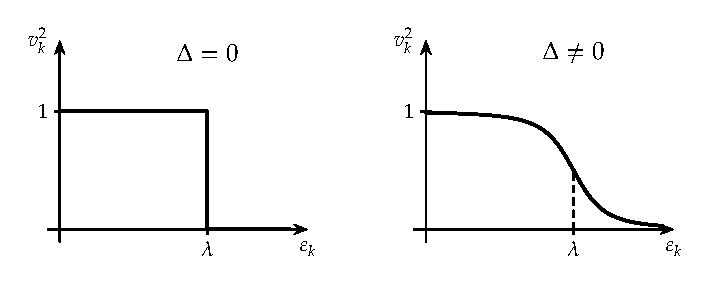
\includegraphics[width=0.7\linewidth]{pictures/6_5}
\par\end{centering}
\centering{}\caption{\label{fig:=0065E0=0076F8=004E92=004F5C=007528=00548C=006709=0076F8=004E92=004F5C=007528=0065F6=007684=005360=00636E=006982=007387}无相互作用$\Delta=0$和有相互作用$\Delta\protect\neq0$时的占据概率}
\end{figure}

\[
\Delta=\frac{G}{2}\sum_{k>0}\frac{\Delta}{\sqrt{(\varepsilon_{k}-\lambda)^{2}+\Delta^{2}}}
\]

在单$j$壳的特殊情况下，所有的$\varepsilon_{k}$都是相等的。从\ref{eq:formal solution of BCS equation G}\ref{eq:tilde epsilon G}和\ref{eq:formal solution of BCS eq}甚至是保留$Gv^{2}_{k}$的情况我们都可以看出，所有的$v^{2}_{k}$都是相等的。从粒子数守恒的条件\ref{eq:particle number expectation}，我们可以得到：
\begin{equation}
v_{k}=\sqrt{\frac{N}{2\Omega}},\quad u_{k}=\sqrt{1-\frac{N}{2\Omega}}\label{eq:v and u G}
\end{equation}

相应的能量（$\varepsilon_{k}=0$）为：
\[
E^{(N)}_{\text{BCS}}=-\frac{1}{2}GN\Omega\left(1-\frac{N}{2\Omega}+\frac{N}{2\Omega^{2}}\right)
\]

这一表达式和精确的结果\ref{eq:E to N}相比，对于大$N$的情况，至少对$1/\Omega$阶的情况是正确的。因此，我们可以说BCS拟设是一个好的近似，非常适合用来处理原子核对关联。

粒子数的不确定度\ref{eq:uncertainty of particle number}也可以从\ref{eq:v and u G}中得到：
\[
\frac{\Delta N}{N}=\frac{1}{\sqrt{N}}\sqrt{2-\frac{N}{\Omega}}
\]

这一模型的能隙可以由\ref{eq:Delta G}和\ref{eq:v and u G}给出：
\[
\Delta=G\sqrt{\frac{N}{2}\left(\Omega-\frac{N}{2}\right)}
\]

因此能隙关于壳中的粒子数是抛物线型的依赖，当壳是空的或者满的的时候，能隙均为零。对于$N=\Omega$，也就是半满壳，我们发现：
\[
2\Delta=G\Omega
\]

我们接下来会看到\ref{subsec:Bogoliubov=0051C6=007C92=005B50=002014=002014=006FC0=0053D1=006001=00548C=00963B=00585E}，$2\Delta$不是偶然的等于第一激发态的能量\ref{eq:energy gap}，随之$\Delta$被称作能隙的原因也会更清晰。

\subsection{Bogoliubov准粒子——激发态和阻塞\label{subsec:Bogoliubov=0051C6=007C92=005B50=002014=002014=006FC0=0053D1=006001=00548C=00963B=00585E}}

把基态写成\ref{eq:BCS wave function}或者\ref{eq:BCS wave function sum form}的形式，除了有和辛弱数模型的精确基态（对的凝聚态）十分相似，因此包含了对关联这一好处之外，还有一个好处就是$|\text{BCS}\rangle$态也可以写成一种新型费米子即Bogoliubov准粒子的直积态。多体物理中的准粒子的概念将会在\ref{chap:=0063A8=005E7F=007684=005355=007C92=005B50=006A21=00578B=00FF08HFB=007406=008BBA=00FF09}中讨论。事实上，可以容易的验证：
\[
|\text{BCS}\rangle\propto\prod_{k}\alpha_{k}|\rangle
\]

这里：
\begin{align}
\alpha^{\dagger}_{k} & =u_{k}a^{\dagger}_{k}-v_{k}a_{\bar{k}}\nonumber \\
\alpha^{\dagger}_{\bar{k}} & =u_{k}a^{\dagger}_{\bar{k}}+v_{k}a_{k}\label{eq:quasi particle operator}
\end{align}

它们满足费米子对易关系：
\[
\{\alpha_{k},\alpha_{k^{\prime}}\}=0;\quad\{\alpha_{k},\alpha^{\dagger}_{k^{\prime}}\}=\delta_{kk^{\prime}}
\]

这里我们通常使用\ref{eq:conj state}和通常的相位约定：
\[
u_{\bar{k}}=u_{k}>0;\quad v_{\bar{k}}=-v_{k}<0;\quad k>0
\]

上式\ref{eq:quasi particle operator}中的拟设和Lipkin模型中的HF-准粒子拟设\ref{eq:Lipkin model operator}非常接近。因此我们可以用相同的技巧来得到解。在Lipkin模型中，我们可以得到实系数（$\varphi=0$）给出了最低能量。在这里，只要$\bar{v}_{k\bar{k}k^{\prime}\bar{k}^{\prime}}<0$，就会出现同样的情况，而这时非常合理的，因此我们只需要使用实系数$u_{k}$和$v_{k}$。

从\ref{eq:quasi particle operator}和\ref{eq:formal solution of BCS eq}我们可以看到，准粒子既有裸粒子的性质，也有裸空穴的性质：在费米面之上（$v^{2}_{k}$很小），它几乎是粒子，而在费米面之下（$u^{2}_{k}$很小），它有几乎是空穴。

从方程\ref{eq:quasi particle operator}可以看出，通过利用线性Bogoliubov变换这个有用的技巧，我们把基态从成对的相互作用粒子表示成了无相互作用准粒子气体。这在很多情况下是非常有用的。而我们必须为之付出的代价则是粒子数不再守恒了——因为我们混合了产生算符和湮灭算符。如果我们假设不仅仅是基态可以由准粒子直积态表示，激发态也可以，那么无相互作用准粒子气体的Hamilton
量$H_{\text{qp}}$则可以表示为：
\[
H_{\text{qp}}=\langle\text{BCS}|H^{\prime}|\text{BCS}\rangle+\sum_{k}E_{k}\alpha^{\dagger}_{k}\alpha_{k}
\]

这里常数$\langle H^{\prime}\rangle$充分考虑了以下事实：
\[
\alpha_{k}|\text{BCS}\rangle=0,\quad\text{对所有的}k
\]

因此，$H_{\text{qp}}$有着正确的基态能量期待值。准粒子能量$E_{k}$是真实粒子相关概念的推广（具体的计算参考\ref{chap:=0063A8=005E7F=007684=005355=007C92=005B50=006A21=00578B=00FF08HFB=007406=008BBA=00FF09}）。
\begin{align*}
E_{k} & =\langle\text{BCS}|\alpha_{k}H^{\prime}\alpha^{\prime}_{k}|\text{BCS}\rangle-\langle\text{BCS}|H^{\prime}|\text{BCS}\rangle\\
 & =\sqrt{\tilde{\varepsilon}^{2}_{k}+\Delta^{2}_{k}}
\end{align*}
 单准粒子态为：
\begin{align*}
\alpha^{\dagger}_{k_{1}}|\text{BCS}\rangle & =a^{\dagger}_{k_{1}}\prod_{k\neq k_{1}}(u_{k}+v_{k}a^{\dagger}_{k}a^{\dagger}_{\bar{k}})|\rangle\\
\alpha^{\dagger}_{\bar{k}_{1}}|\text{BCS}\rangle & =a^{\dagger}_{\bar{k}_{1}}\prod_{k\neq k_{1}}(u_{k}+v_{k}a^{\dagger}_{k}a^{\dagger}_{\bar{k}})|\rangle
\end{align*}

这些态显然有能量为$\langle H^{\prime}\rangle+E_{k}$。它们是具有奇数粒子数的一系列态的叠加，描述了奇核。根据量子数$k_{1}$，这一态既可能是基态，也可能是激发态\footnote{什么意思？可能是奇核的基态或者偶核的激发态？}。

两粒子准粒子态：
\begin{align*}
\alpha^{\dagger}_{k_{1}}\alpha^{\dagger}_{k_{2}}|\text{BCS}\rangle & =a^{\dagger}_{k_{1}}a^{\dagger}_{k_{2}}\prod_{k\neq k_{1},k_{2}}(u_{k}+v_{k}a^{\dagger}_{k}a^{\dagger}_{\bar{k}})|\rangle,\quad k_{2}\neq\bar{k}_{1}\\
\alpha^{\dagger}_{k_{1}}\alpha^{\dagger}_{\bar{k}_{1}}|\text{BCS}\rangle & =(-v_{k_{1}}+u_{k_{1}}a^{\dagger}_{k_{1}}a^{\dagger}_{\bar{k}_{1}})\prod_{k\neq k_{1}}(u_{k}+v_{k}a^{\dagger}_{k}a^{\dagger}_{\bar{k}})|\rangle,\quad k_{2}=\bar{k}_{1}
\end{align*}

它们具有能量$\langle H^{\prime}\rangle+E_{k_{1}}+E_{k_{2}}$。它们描述了偶核的激发态。在这种情况下，有一个对被拆开了，激发能为：
\[
E_{k_{1}}+E_{k_{2}}\ge2\Delta
\]

偶核的第一激发态的能量因此一定比基态能量高出$2\Delta$以上。

在只有一个$j$-壳的情况下，激发能为：
\[
E_{k}+E_{k^{\prime}}=2\sqrt{\tilde{\varepsilon}^{2}+\Delta^{2}}
\]

考虑纯对力的情况，再令$\varepsilon_{k}=0$
\begin{comment}
令$\varepsilon_{k}=0$相当于辛弱数模型。
\end{comment}
，得到：

\[
\tilde{\varepsilon}=G\frac{\Omega-N}{2}
\]

\begin{booknote*}
利用$v^{2}_{k}$的表达式\ref{eq:formal solution of BCS equation G}，得到：
\[
\lambda^{2}=\frac{(2v^{2}_{k}-1)^{2}\Delta^{2}}{1-(2v^{2}_{k}-1)^{2}}
\]

再代入上一节得到的$v^{2}_{k}$和$\Delta$的表达式，得到：
\[
\lambda^{2}=\frac{G^{2}}{4}(N-\Omega)^{2}
\]

由于此时$\tilde{\varepsilon}=-\lambda$，而$\tilde{\varepsilon}$一定为正，所以得到$\tilde{\varepsilon}=G\frac{\Omega-N}{2}$。
\end{booknote*}
从而得出：

\[
E_{k}+E_{k^{\prime}}=G\cdot\Omega
\]

和辛弱数模型得到的结果\ref{eq:energy gap}相符
\begin{comment}
但这是省略了$Gv^{2}_{k}$和$Gv^{4}_{k}$得到的结果。
\end{comment}
。此外由准粒子能$\tilde{\varepsilon}$的表达式我们还可以发现，只有半满壳的时候，激发能才为$2\Delta$。

在基态奇粒子数的系统里，激发态为$\alpha^{\dagger}_{k}|\text{BCS}\rangle$，基态为$\alpha_{k_{0}}|\text{BCS}\rangle$，如果$\tilde{\varepsilon}_{k_{0}}\simeq0$，则激发能为：
\[
E_{k}-E_{k_{0}}=\sqrt{\tilde{\varepsilon}^{2}_{k}+\Delta^{2}}-\Delta
\]

如果$\tilde{\varepsilon}_{k}\ll\Delta$，上式基本为零，我们因此发现在这些奇粒子数系统中能级密度非常大。

我们也可以用如下的方式解释奇偶质量效应：对于任意的$N$，基态能量$E^{\text{GS}}_{N}$可以如下给出：
\[
E^{\text{GS}}_{N+2}=E^{\text{GS}}_{N}+2\lambda;\quad E^{\text{GS}}_{N+1}=E^{\text{GS}}_{N}+\lambda+E_{k_{0}}
\]

因此奇偶质量差为：
\[
\frac{1}{2}[E^{\text{GS}}_{N+2}-E^{\text{GS}}_{N+1}-(E^{\text{GS}}_{N+1}-E^{\text{GS}}_{N})]=-E_{k_{0}}\simeq-\Delta
\]

上式经常用来从实验上测得的结合能确定能隙。现在已经发现，平均来讲能隙和核子数的关系为$\Delta=12\cdot A^{-1/2}$\cite{NA62,ZGS67}，如\ref{fig:=008D28=005B50=0080FD=009699=00968F=008D28=005B50=006570=007684=0053D8=005316(=00005BBM-69=00005D)}。

\begin{figure}[H]
\begin{centering}
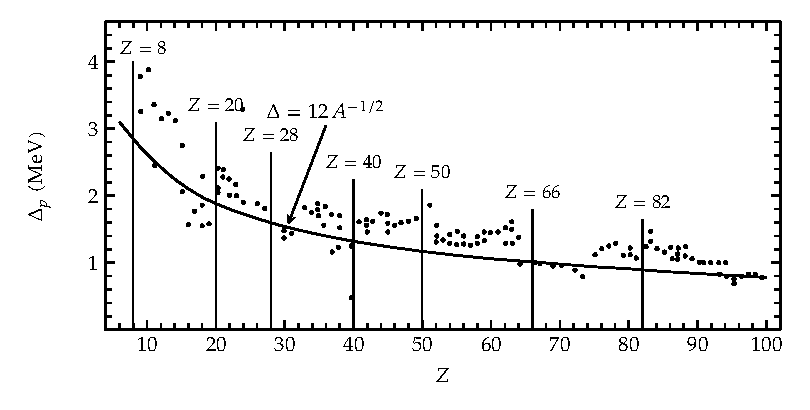
\includegraphics[width=0.6\linewidth]{pictures/6_6}
\par\end{centering}
\centering{}\caption{\label{fig:=008D28=005B50=0080FD=009699=00968F=008D28=005B50=006570=007684=0053D8=005316(=00005BBM-69=00005D)}质子能隙随质子数的变化(\cite{BM69})}
\end{figure}

上述讨论使我们对超流核中许多态的结构获得了定性的理解。然而，在更深入的细致研究中，还有几个重要的要点必须予以考虑：

\textbf{(i) 化学势}（The Chemical Potential）。正如在式\ref{eq:particle number expectation}中所见，化学势$\lambda$的确定是为了使
BCS 基态中的平均粒子数具有正确的数值。利用同一个$\lambda$，对于单准粒子态$|k\rangle=\alpha^{\dagger}_{k}|\text{BCS}\rangle$，我们发现
\begin{equation}
\langle k|\hat{N}|k\rangle=N+u^{2}_{k}-v^{2}_{k}\label{eq:average_particle_number_quasi}
\end{equation}
只有对于远离 Fermi 面的能级$k$，上式才等于$N\pm1$。对于 Fermi 面附近的能级，平均粒子数是不正确的。由于能量对平均粒子数具有强烈的依赖性，因此应当针对奇核中的不同能级以及偶核中的激发能级重新调整化学势$\lambda$。只要我们尚未进行这种重新调整，就应当在计算激发能时使用算符$H^{\prime}=H-\lambda\hat{N}$而不是$H$（正如我们目前所做的那样）。例如，如果我们对式\ref{eq:average_particle_number_quasi}中态$|k\rangle$不正确的粒子数进行修正，就可以看出这一点：
\begin{align*}
E^{k}_{N+1} & =\langle k|H|k\rangle+\frac{\mathrm{d}E}{\mathrm{d}N}(N+1-\langle k|\hat{N}|k\rangle)\\
 & =\langle k|H-\lambda\hat{N}|k\rangle+\lambda(N+1)\\
 & =E^{\text{GS}}_{N}+\lambda+E_{k}
\end{align*}

\textbf{(ii) 阻塞效应}（The Blocking Effect）。BCS 基态的占据概率$v^{2}_{k}${[}式\ref{eq:formal solution of BCS eq}{]}
是由变分原理决定的。奇核系统的基态由如下波函数描述：
\begin{equation}
\alpha^{\dagger}_{k_{1}}|\text{BCS}\rangle=a^{\dagger}_{k_{1}}\prod_{k\neq k_{1}}(u_{k}+v_{k}a^{\dagger}_{k}a^{\dagger}_{\bar{k}})|-\rangle\label{eq:blocked_wavefunction}
\end{equation}
未配对的粒子处在能级$k_{1}$上并将该能级“阻塞”。Pauli 原理阻止了该能级参与由对关联引起的核子散射过程。能级$k_{1}$始终保持被占据，而能级$\bar{k}_{1}$则始终保持为空。只有对于$k\neq k_{1}$，我们才有$v^{2}_{k}=v^{2}_{\bar{k}}$（\ref{fig:=0072B6=006001k1=007684=00963B=00585E}）。将受阻塞的波函数\ref{eq:blocked_wavefunction}作为试探波函数用于变分原理，我们得到与之前相同的关于$v^{2}_{k}$的方程。唯一的区别在于，在能隙的计算中有一个能级被“阻塞”：
\begin{equation}
\Delta=G\sum_{k\neq k_{1}}u_{k}v_{k}\label{eq:blocked_gap}
\end{equation}
能级$k_{1}$必须从求和中排除，因为它无法对配对能量做出贡献。化学势由下式决定：
\begin{equation}
N=1+2\sum_{k\neq k_{1}}v^{2}_{k}\label{eq:blocked_particle_number}
\end{equation}
对于存在更多阻塞能级的情况（例如双准粒子态），完全类似的方程同样成立。

\begin{figure}[H]
\begin{centering}
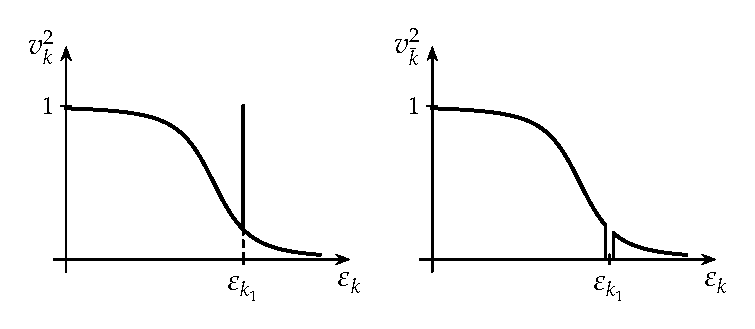
\includegraphics[width=0.85\linewidth]{pictures/6_7}
\par\end{centering}
\centering{}\caption{\label{fig:=0072B6=006001k1=007684=00963B=00585E}状态$k_{1}$的阻塞}
\end{figure}

$\Delta$以及$u_{k}$与$v_{k}$的这种改变称为阻塞效应。这些阻塞关联是$\Omega^{-1}$量级的，通常可以忽略。然而，正如
Soloviev \cite{So61,Wa62b} 以及 Nilsson 和 Prior \cite{NP61} 所指出的，在某些情况下这一修正可能相当大。这在形变核中尤为突出，因为在形变核的能谱中尽管可能有
20 个能级，但对式\ref{eq:gap equation}的求和有显著贡献的仅有 4 或 5 个能级。显然，在这样的情形下阻塞其中一两个能级会产生巨大的影响，以至于人们不能简单地将激发能等同于准粒子能量，而必须计算激发态的总能量并减去真空态能量。对于双准粒子态，修正后的能量（$\simeq1.4\,\text{MeV}$）总是小于准粒子能量（$\simeq1.7\,\text{MeV}$），但远大于自由粒子能量（$\simeq0.15\,\text{MeV}$）。在这种修正理论中产生的一个问题是，$v_{k}$在基态和激发态中可能存在显著差异，导致这些态不再自动正交，尽管有时不同的量子数（如自旋或宇称）能够保证正交性。特别是，在这些情况下自旋为$0^{+}$的双准粒子态与基态并不正交。

\subsection{能隙方程的讨论\label{subsec:=0080FD=009699=0065B9=007A0B=007684=008BA8=008BBA}}

在所有实际应用中，BCS 方程都必须借助计算机进行数值求解，于是就产生了一个问题：在计算中应当包含多少个能级？也就是说，我们必须探究哪些状态对能隙方程\ref{eq:gap equation}中出现的求和贡献最大。为此，让我们首先考虑靠近
Fermi 能级的某个状态的能隙$\Delta_{k}$。在这种情况下，求和的主要贡献来自 Fermi 能级附近的状态。其原因在于：(i)
在此情形下，表达式$\Delta_{k^{\prime}}/(\tilde{\varepsilon}^{2}_{k^{\prime}}+\Delta^{2}_{k^{\prime}})^{1/2}\simeq1$（因为$\tilde{\varepsilon}_{k^{\prime}}\simeq0$）；(ii)
当$k^{\prime}\simeq k$时（波函数具有强重叠），矩阵元$\bar{v}_{k\bar{k}k^{\prime}\bar{k}^{\prime}}$比其他矩阵元更大。

反之，若$k$远离 Fermi 面，则式\ref{eq:gap equation}求和中的所有项都很小。对于$k^{\prime}\simeq k$，波函数的重叠虽然仍然很大，但由于$\tilde{\varepsilon}^{2}_{k}\gg\Delta^{2}_{k}$，因子$\Delta_{k^{\prime}}/(\tilde{\varepsilon}^{2}_{k^{\prime}}+\Delta^{2}_{k^{\prime}})^{1/2}$此时变得很小。而对于
Fermi 面上的状态$k^{\prime}$，情况恰好相反，因为那里的矩阵元非常小（$k$与$k^{\prime}$通常属于不同的主量子数）。

因此，配对力的效应局限于 Fermi 面的邻域，也就是说，仅在这一邻域内$\Delta_{k}$才显著不为零。现在我们便能理解，为什么在
Fermi 面邻域取常数配对力而在其余区域矩阵元取为零是一个合理的近似。另一方面，如果我们在整个组态空间中都取常数矩阵元，则能隙将会发散。

对于球形或仅弱形变的原子核，单粒子能级呈现出显著的壳层结构。能隙方程求和中的主要贡献来自于同一壳层内的跃迁。因此，我们或多或少可以分别独立处理各个壳层。由上述讨论，我们预期对于内壳层有$\Delta_{k}\simeq0$。因此，配对力仅在部分填充的壳层中有效，该壳层通常称为$\Lambda$壳层（$\Lambda$-shell）。这便回到了辛弱数模型。对于强形变核，壳层结构已被完全抹平，尽管如此，求和依然仅仅遍及
Fermi 面邻近的一组能级，这组能级同样称为$\Lambda$壳层。

配对效应局限于 Fermi 能级附近，这也是中子与质子可以分别独立处理的原因（至少对于重核而言）。对于$A\sim150$的原子核，过剩中子数为$(N-Z)\geqslant20$。因此，靠近
Fermi 能级的中子与质子能级之间的重叠，与纯质子或纯中子能级之间的重叠相比非常小。因此，忽略中子-质子配对，总波函数可以表示为质子部分与中子部分的直积：
\begin{equation}
|\text{BCS}\rangle=\prod_{k_{1}>0}\left(u^{(p)}_{k_{1}}+v^{(p)}_{k_{1}}a^{(p)\dagger}_{k_{1}}a^{(p)\dagger}_{\bar{k}_{1}}\right)\prod_{k_{2}>0}\left(u^{(n)}_{k_{2}}+v^{(n)}_{k_{2}}a^{(n)\dagger}_{k_{2}}a^{(n)\dagger}_{\bar{k}_{2}}\right)|-\rangle\label{eq:bcs_proton_neutron}
\end{equation}

尽管引入了这些简化假设，BCS 方程通常仍只能通过数值计算求解。为了定性地研究核子对之间相互作用的影响，我们将自身限制于$\Lambda$壳层内的纯配对力\ref{eq:pure pair force energy expectation}。在接下来的讨论中，我们因而忽略其他壳层。此时能隙方程具有如下形式：
\begin{equation}
\Delta=\frac{1}{2}G\sum^{\Lambda}_{k>0}\frac{\Delta}{\sqrt{\tilde{\varepsilon}^{2}_{k}+\Delta^{2}}}\label{eq:gap_equation_lambda_shell}
\end{equation}
其中求和仅遍历$\Lambda$壳层。方程\ref{eq:gap_equation_lambda_shell}总是存在平凡解$\Delta=0$，即$u_{k}\cdot v_{k}=0$；在不存在配对力或配对力足够弱时，这是唯一的解。然而，当满足条件
\begin{equation}
\frac{1}{2}G\sum^{\Lambda}_{k>0}\frac{1}{|\tilde{\varepsilon}_{k}|}>1\label{eq:nontrivial_gap_condition}
\end{equation}
时，存在第二个非平庸解$\Delta>0$。只要配对力足够强，或者$\Lambda$壳层足够大，这种情况总会发生。然而，这一突变的相变是粒子数不守恒（粒子数破缺）的结果，在更扩展的理论
\cite{MPR65} 中它在某种程度上会被抹平平滑化。对于无限大系统，粒子数破缺是可以忽略的，此时相变总是尖锐突变的。

另一方面，式\ref{eq:gap_equation_lambda_shell}也可用于确定配对力的强度$G$，因为正如我们之前所述，$\Delta$可以从奇偶效应经验地确定。然而，它仍然依赖于“截断”（cutoff）$\Lambda$。

\subsection{能隙方程的示意解\label{subsec:=0080FD=009699=0065B9=007A0B=007684=00793A=00610F=0089E3}}

获得能隙方程的解析解是非常富有启发性的 \cite{Be59}。这只能在一个非常简化的示意模型中实现。我们设想一个具有良好形变的原子核，其能级密度近似均匀，且平均能级间距$\Delta\varepsilon$远小于$\Delta$（对于稀土区的形变核，$\Delta\simeq1\,\text{MeV}$，而$\Delta\varepsilon\simeq0.1\text{--}0.2\,\text{MeV}$）。于是我们可以近似地将式\ref{eq:gap_equation_lambda_shell}中的求和替换为在$\Lambda$壳层上的积分：$\varepsilon^{\prime}<\varepsilon<\varepsilon^{\prime\prime}$；令$a=\varepsilon^{\prime}-\lambda$，$b=\varepsilon^{\prime\prime}-\lambda$，有
\begin{equation}
1=\frac{1}{2}G\int^{b}_{a}\frac{1}{\sqrt{\varepsilon^{2}+\Delta^{2}}}\rho(\varepsilon)\,\mathrm{d}\varepsilon\label{eq:schematic_gap_integral}
\end{equation}
其中$\rho(\varepsilon)$为能级密度。我们进一步假设$\rho(\varepsilon)$在$\Lambda$壳层内近似为常数（$\rho\simeq\bar{\rho}$）。引入无量纲量
\begin{equation}
\eta=\frac{1}{\bar{\rho}G}\label{eq:eta_definition}
\end{equation}
积分后可得
\begin{equation}
2\eta=\operatorname{arsinh}\frac{b}{\Delta}-\operatorname{arsinh}\frac{a}{\Delta}\label{eq:arsinh_relation}
\end{equation}
解出$\Delta$可得
\begin{equation}
\Delta=\frac{1}{\sinh2\eta}\sqrt{b^{2}+a^{2}-2ab\cosh2\eta}\label{eq:delta_schematic_solution}
\end{equation}
BCS 模型中的平均粒子数由式\ref{eq:particle number expectation}给出，并由此确定化学势$\lambda$。$\Lambda$壳层内的粒子数由下式给出（我们再次将式\ref{eq:particle number expectation}中的求和替换为积分）：
\begin{equation}
N=2\int^{b}_{a}\frac{1}{2}\left(1-\frac{\varepsilon}{\sqrt{\varepsilon^{2}+\Delta^{2}}}\right)\bar{\rho}\,\mathrm{d}\varepsilon\label{eq:particle_number_schematic}
\end{equation}
$\Lambda$壳层内的能级数由下式给出：
\begin{equation}
\Omega=\bar{\rho}(b-a)\label{eq:omega_levels}
\end{equation}
引入占据因子
\begin{equation}
\chi_{N}=1-\frac{N}{\Omega}\label{eq:chi_n_definition}
\end{equation}
利用式\ref{eq:delta_schematic_solution}，经过冗长但直接的计算，可得
\begin{equation}
\lambda=\frac{\varepsilon^{\prime}+\varepsilon^{\prime\prime}}{2}-\frac{\varepsilon^{\prime\prime}-\varepsilon^{\prime}}{2}\chi_{N}\operatorname{ctgh}\eta\label{eq:lambda_schematic}
\end{equation}
将式\ref{eq:lambda_schematic}代入式\ref{eq:delta_schematic_solution}，得到：
\begin{equation}
\Delta=\frac{\varepsilon^{\prime\prime}-\varepsilon^{\prime}}{2\sinh\eta}\sqrt{1-\chi^{2}_{N}}\label{eq:delta_chi_n}
\end{equation}
在弱耦合极限下，即对于$G\cdot\bar{\rho}\ll1$，我们发现：
\begin{equation}
\Delta\propto\mathrm{e}^{-(1/\bar{\rho}G)}\label{eq:delta_exponential_weak}
\end{equation}
因此，从式\ref{eq:delta_exponential_weak}可以得到一个重要结论：能隙不能按相互作用强度的幂级数展开。

式\ref{eq:delta_chi_n}是在$\Delta$不小于能级间距的条件下导出的，即
\begin{equation}
\Delta\cdot\bar{\rho}>1\label{eq:delta_rho_condition}
\end{equation}
或者
\begin{equation}
\frac{1}{2\sinh\eta}\sqrt{N(2\Omega-N)}>1\label{eq:delta_rho_condition_explicit}
\end{equation}
对于$\eta\ll1$（强配对关联），该不等式总是满足的。对于$\eta\gg1$，式\ref{eq:delta_rho_condition_explicit}仅在$N(2\Omega-N)$的值足够大时才成立。

BCS 理论中的基态能量由式\ref{eq:pure pair force energy expectation}给出。它对$H^{\prime}$的基态期望值的贡献为
\begin{equation}
\langle\text{BCS}|H^{\prime}|\text{BCS}\rangle=2\int^{b}_{a}\frac{1}{2}\left(1-\frac{\varepsilon}{\sqrt{\varepsilon^{2}+\Delta^{2}}}\right)\varepsilon\bar{\rho}\,\mathrm{d}\varepsilon-\frac{\Delta^{2}}{G}\label{eq:h_prime_expectation}
\end{equation}
由于$H^{\prime}$与$H$相差$\lambda\cdot N$，利用式\ref{eq:lambda_schematic}并完成式\ref{eq:h_prime_expectation}中的积分，我们得到基态能量：
\begin{equation}
E_{\text{BCS}}=\langle\text{BCS}|H|\text{BCS}\rangle=\frac{1}{2}(\varepsilon^{\prime\prime}+\varepsilon^{\prime})N-\frac{1}{4}\Omega(\varepsilon^{\prime\prime}-\varepsilon^{\prime})(1-\chi^{2}_{N})\operatorname{ctgh}\eta\label{eq:e_bcs_energy}
\end{equation}
我们关注的是基态能量中单纯来自配对力的那一部分。为此，我们首先计算$G=0$时的能量，这对应于极限$\eta\to\infty$：
\begin{equation}
E^{0}=\frac{1}{2}(\varepsilon^{\prime}+\varepsilon^{\prime\prime})\cdot N-\frac{1}{4}\Omega(\varepsilon^{\prime\prime}-\varepsilon^{\prime})(1-\chi^{2}_{N})\label{eq:e_zero_energy}
\end{equation}
因此，配对力对基态能量的贡献$E^{P}$由下式给出：
\begin{equation}
E^{P}=E_{\text{BCS}}-E^{0}\label{eq:e_p_definition}
\end{equation}
在半满壳层（即$N=\Omega$）的情形下，利用式\ref{eq:e_bcs_energy}、式\ref{eq:e_zero_energy}、式\ref{eq:omega_levels}和式\ref{eq:delta_chi_n}，可得
\begin{equation}
E^{P}=-\frac{1}{4}\Omega(\varepsilon^{\prime\prime}-\varepsilon^{\prime})(1-\chi^{2}_{N})(\operatorname{ctgh}\eta-1)=-\frac{1}{2}\Delta^{2}\bar{\rho}(1-\mathrm{e}^{-2\eta})\label{eq:e_p_half_filled}
\end{equation}
这就是中子或质子的配对能（pairing energy）。对于重核，可以从奇偶效应估计$G$和$\Delta$。Nilsson
和 Prior \cite{NP61} 发现，对于质子$G_{p}\simeq17/A\,\text{MeV}$，对于中子$G_{n}\simeq25/A\,\text{MeV}$。能隙$\Delta$约为$1\,\text{MeV}$。假设特征能级密度为$1/\bar{\rho}\simeq0.5\,\text{MeV}$，可得$\eta\simeq A/100$。在此情形下，我们可以忽略式\ref{eq:e_p_half_filled}中的$\mathrm{e}^{-2\eta}$项，从而得到总配对能（质子和中子的配对能大致相同）：
\begin{equation}
E^{P}_{\text{total}}=E^{P}_{(p)}+E^{P}_{(n)}\simeq-\bar{\rho}\Delta^{2}\simeq-2\,[\text{MeV}]\label{eq:e_total_pairing}
\end{equation}
因此，与总结合能相比，总配对能极其微小。这是各类关联能的普遍特征，然而，这绝不意味着它们在解释许多物理问题时不能发挥决定性的作用。

正如我们所见，BCS 波函数所代表的态并不是粒子数算符的本征态。整个理论仅在$|\text{BCS}\rangle$很好地定域于实际粒子数附近时才有效。为了获得一个估计，我们计算粒子数的均方偏差\ref{eq:uncertainty of particle number}：
\begin{equation}
(\Delta N)^{2}=\sum_{k>0}\frac{\Delta^{2}_{k}}{\tilde{\varepsilon}^{2}_{k}+\Delta^{2}_{k}}\label{eq:delta_n_squared_definition}
\end{equation}
在示意模型中，由此可得
\begin{equation}
(\Delta N)^{2}=\bar{\rho}\Delta\left(\arctan\frac{b}{\Delta}-\arctan\frac{a}{\Delta}\right)\label{eq:delta_n_squared_schematic}
\end{equation}
在弱配对关联或低能级密度的极限下，我们得到
\begin{equation}
(\Delta N)^{2}=\bar{\rho}\cdot\Delta\cdot\pi\label{eq:delta_n_weak_pairing}
\end{equation}
这一近似对于强形变核大体上是满足的。取$\bar{\rho}$和$G$的典型特征值，我们得到$\eta\simeq4,\dots,5$，平均偏差为$\Delta N\simeq\sqrt{6}$。

在强配对的另一极限下（$\eta\ll1$），我们仅保留式\ref{eq:delta_n_squared_schematic}关于$\eta$的领头项：
\begin{equation}
(\Delta N)^{2}=\Omega(1-\chi^{2}_{N})=2N\left(1-\frac{N}{2\Omega}\right)\label{eq:delta_n_strong_pairing}
\end{equation}
因此，对于半满壳层（$N=\Omega$），可得$\Delta N=\sqrt{N}$；而对于仅有一对核子（$N=2$），我们得到$\Delta N\simeq2$。$\eta\ll1$的半满壳层的一个典型例子是$^{202}\text{Pb}$。其
BCS 波函数包含大量的$^{204}\text{Pb}$和$^{200}\text{Pb}$，以及$^{206}\text{Pb}$和$^{198}\text{Pb}$。然而我们必须记住，对于所有这些核，Fermi
面$\lambda$和能隙$\Delta$几乎完全相同，因此粒子数的不确定性并不像表面上看起来那么严重。

正如我们所看到的，非常简单的 BCS 模型使我们能够解释核子短程关联所引起的原子核的许多特征。我们仅分别独立处理了中子和质子的配对，忽略了中子-质子相互作用。对于重核，这是合理的，因为质子和中子波函数通常属于不同的主量子数，配对矩阵元很小。然而对于轻核（$s\text{--}d$壳层！），这不再成立，我们还必须计入中子-质子配对。在非常简要地提及其中某些计算之前，我们希望从更一般的
Hartree-Fock-Bogoliubov 理论重新审视 Hartree-Fock 理论、形变以及配对，正如我们将看到的，该理论涵盖了我们迄今所讨论的所有模型。



\chapter{推广的单粒子模型（HFB理论）\label{chap:=0063A8=005E7F=007684=005355=007C92=005B50=006A21=00578B=00FF08HFB=007406=008BBA=00FF09}}

\section{导论}

正如我们在前两章所看到的，原子核的许多性质，都可以通过独立粒子模型描述，该模型中引入了一个强烈依赖于物质分布的平均场，独立的核子在其中运动。我们发现，在半满壳中粒子之间有额外的关联。而在BCS模型中我们学会了利用推广的单粒子图像来处理这些关联，只需引入准粒子和一种新的场——对场。

Hartree-Fock-Bogoliubov（HFB）理论推广并统一了这两种方法。在这个理论中我们寻找由独立运动的准粒子组成的最一般的乘积波函数。准粒子的波函数通过变分原理确定，并且在静态的单粒子图像的前提下考虑了尽可能多的关联。事实证明，在这个近似中，Hamilton
量简化为两个平均势，即我们已经从 Hartree-Fock 理论中知道的自洽场$\Gamma$，以及从 BCS 理论中知道的对场$\Delta$。自洽场$\Gamma$包含所有最终导致形变基态（相变）的长程ph关联。另一方面，$\Delta$包含了所有可能导致相变和超流态的短程对关联。HFB理论现在统一了这两种描述，并处理了它们的相互依存关系。因此，它有能力同时处理平均场近似下的所有可能的相变。

由于HFB理论是Hartree-Fock理论和BCS理论的结合，因此许多相关问题在前面的章节中已经讨论过。因此，我们可以用相当形式化的方式推导出本章开头出现的必要公式。在第
7.2 节中，我们介绍了一个一般的准粒子图像。所研究的核波函数被定义为合适的准粒子算子的真空，并讨论了其形式性质。在这种情况下，我们在附录
E中证明了许多公式和一些重要的定理。在7.3 节中，我们推导出了确定波函数的 HFB 方程，并提出了几种求解它们的方法。在第 7.4
节中我们介绍了对-四极模型
\begin{comment}
pairing-plus-quadrupole model不知道叫什么名字。
\end{comment}
作为示例，该模型显示了实际计算的许多重要特征。最后几节讨论了该理论的几个应用，一个是形变核基态性质的约束Hartree-Fock理论（CHF）计算，用于研究裂变背景下的能量面，另外一个是自洽Cranking（SCC）模型下转动谱的计算。

\section{推广的Bogoliubov变换}

\subsection{准粒子算符}

任何准粒子概念的基本思想都是将原子核的基态表示为准粒子真空，准粒子由相邻原子核的低能激发态定义。这正是Landau和Migdal {[}La
59，Mi 67{]}的概念，他们根据多体系统的精确本征态来定义真空和准粒子。因此，费米液体的这个理论原则上是一个精确的理论；然而，它的一个重要缺点是这些Landau-Migdal准粒子与系统的“裸”粒子（由一些基本的算符$c^{\dagger}_{l}$，$c_{l}$给出，例如，可能是平面波态或谐振子态）之间没有简单的数学关系。

在本章中，我们使用了所谓的Bogoliubov准粒子{[}Bo 58，Bo 59a+b，BS 59，Va 61{]}，它与裸粒子具有线性关系。它们很容易处理，但相应的真空和单粒子态现在只是多体
Hamilton 量的精确本征态的近似。

我们已经在BCS模型中定义了一种非常特殊类型的准粒子（方程6.67）。在对关联消失的极限下（$u_{k},v_{k}=0$）中，它们要么是粒子（$\varepsilon_{k}>\varepsilon_{\text{F}}$）要么是空穴（$\varepsilon_{k}\leq\varepsilon_{\text{F}}$）。这些BCS准粒子的自然拓展是由从裸粒子算符$c^{\dagger}_{l}$，$c_{l}$到准粒子算符$\beta^{\dagger}_{k}$，$\beta_{k}$的最一般线性变换给出的：
\[
\beta^{\dagger}_{k}=\sum_{l}U_{lk}c^{\dagger}_{l}+V_{lk}c_{l}
\]

指标$k$和$l$取遍整个组态空间（$k=1,\dots,M$）。方程的厄米共轭给出算符$\beta_{k}$。我们因此得到了一个从$2M$维空间上的算符$(c_{1}\dots c_{M},c^{\dagger}_{1}\dots c^{\dagger}_{M})$到算符$(\beta_{1}\dots\beta_{M},\beta^{\dagger}_{1}\dots\beta^{\dagger}_{M})$的变换（方程（7.2）中矩阵的定义似乎有些不寻常;然而，它与定义（7.1）一致，并且使得我们可以在下面使用矩阵乘法规则。）：
\[
\begin{bmatrix}\beta\\
\beta^{\dagger}
\end{bmatrix}=\begin{bmatrix}U^{\dagger} & V^{\dagger}\\
V^{\mathrm{T}} & U^{\mathrm{T}}
\end{bmatrix}\begin{bmatrix}c\\
c^{\dagger}
\end{bmatrix}=\mathcal{W}^{\dagger}\begin{bmatrix}c\\
c^{\dagger}
\end{bmatrix}
\]

这一变换由矩阵$\mathcal{W}$表征：
\[
\mathcal{W}=\begin{bmatrix}U & V^{*}\\
V & U^{*}
\end{bmatrix}
\]

现在系数$U$和$V$并不完全是任意的，因为新算符$\beta_{k}$，$\beta^{\dagger}_{k}$需要满足和之前相同的费米对易关系。这使得矩阵$\mathcal{W}$必须是酉矩阵。
\[
\mathcal{W}^{\dagger}\mathcal{W}=1\quad\text{和}\quad\mathcal{W}\mathcal{W}^{\dagger}=1
\]

或者可以写为：
\begin{align}
U^{\dagger}U+V^{\dagger}V & =1\label{eq:orthogonality of UV}\\
UU^{\dagger}+V^{*}V^{\mathrm{T}} & =1\nonumber \\
U^{\mathrm{T}}V+V^{\mathrm{T}}U & =0\nonumber \\
UV^{\dagger}+V^{*}U^{\mathrm{T}} & =0\nonumber 
\end{align}

这使得我们可以写出逆变换：
\[
c^{\dagger}_{l}=\sum_{k}U^{*}_{lk}\beta^{\dagger}_{k}+V_{lk}\beta_{k}
\]

Bloch和Messiah有一个著名的定理{[}Zu 62，BM 62{]}，它指出，形式的（7.3）的酉矩阵总是可以分解为三个非常特殊形式的矩阵：
\begin{equation}
\mathcal{W}=\begin{bmatrix}D & 0\\
0 & D^{*}
\end{bmatrix}\begin{bmatrix}\bar{U} & \bar{V}\\
\bar{V} & \bar{U}
\end{bmatrix}\begin{bmatrix}C & 0\\
0 & C^{*}
\end{bmatrix}\label{eq:decomposition of W}
\end{equation}

或者写为：
\begin{align*}
U & =D\bar{U}C\\
V & =D^{*}\bar{V}C
\end{align*}

这里$D$和$C$是酉矩阵，$\bar{U}$和$\bar{V}$是具有如下形式的实矩阵：

\begin{align}
\bar{U} & =\left[\begin{array}{rrrrrrr}
\ddots\\
 & 0 &  &  &  & 0\\
 &  & \begin{array}{cc}
\text{\makebox[0pt]{\ensuremath{u_{1}}}} & 0\\
0 & \text{\makebox[0pt]{\ensuremath{u_{1}}}}
\end{array}\\
 &  &  & \ddots\\
 &  &  &  & \begin{array}{cc}
\text{\makebox[0pt]{\ensuremath{u_{n}}}} & 0\\
0 & \text{\makebox[0pt]{\ensuremath{u_{n}}}}
\end{array}\\
 & 0 &  &  &  & 1\\
 &  &  &  &  &  & \ddots
\end{array}\right]\label{eq:form of UV}\\
\bar{V} & =\left[\begin{array}{rrrrrrr}
\ddots\\
 & 1 &  &  &  & 0\\
 &  & \begin{array}{cc}
0 & \text{\makebox[0pt]{\ensuremath{v_{1}}}}\\
\text{\makebox[0pt]{\ensuremath{-v_{1}}}} & 0
\end{array}\\
 &  &  & \ddots\\
 &  &  &  & \begin{array}{cc}
0 & \text{\makebox[0pt]{\ensuremath{v_{n}}}}\\
\text{\makebox[0pt]{\ensuremath{-v_{n}}}} & 0
\end{array}\\
 & 0 &  &  &  & 0\\
 &  &  &  &  &  & \ddots
\end{array}\right]\nonumber 
\end{align}

\begin{booknote*}
然而使用下面这种形式的矩阵会使得证明更加简单，也没有本质区别：

\[
\bar{V}=\left[\begin{array}{rrrrrrrr}
\ddots\\
 & 0 & \makebox[0pt]{\ensuremath{1}} &  &  &  & 0\\
 & \makebox[0pt]{\ensuremath{-1}} & \text{0}\\
 &  &  & \begin{array}{cc}
0 & \text{\makebox[0pt]{\ensuremath{v_{1}}}}\\
\text{\makebox[0pt]{\ensuremath{-v_{1}}}} & 0
\end{array}\\
 &  &  &  & \ddots\\
 &  &  &  &  & \begin{array}{cc}
0 & \text{\makebox[0pt]{\ensuremath{v_{n}}}}\\
\text{\makebox[0pt]{\ensuremath{-v_{n}}}} & 0
\end{array}\\
 & 0 &  &  &  &  & 0\\
 &  &  &  &  &  &  & \ddots
\end{array}\right]
\]
\end{booknote*}
这个定理的证明在附录E.1中给出。这个定理意味着这个变换可以分解成三个部分：
\begin{align*}
\begin{array}{ccc}
\left.\begin{array}{cc}
c & \rightarrow a\\
c^{\dagger} & \rightarrow a^{\dagger}
\end{array}\right\}  & \longrightarrow & \left\{ \begin{array}{cc}
\alpha & \rightarrow\beta\\
\alpha^{\dagger} & \rightarrow\beta^{\dagger}
\end{array}\right.\\
D & \bar{U},\bar{V} & C
\end{array}
\end{align*}

\begin{enumerate}
\item 一个粒子算符$c^{\dagger}$内部的酉变换，跟HF的情形一样：
\[
a^{\dagger}_{k}=\sum_{l}D_{lk}c^{\dagger}_{l}
\]

它定义了一组新的基，叫正则基（叫这个名字是因为反对称对张量$\kappa$在这组基下是正则形式。），在附录E中有更详细的解释。它很方便使用，因为在这组基下密度矩阵$\rho$是对角的。
\item 一个特殊的Bogoliubov变换，
\begin{align}
\alpha^{\dagger}_{p} & =u_{p}a^{\dagger}_{p}-v_{p}a_{\bar{p}}\nonumber \\
\alpha^{\dagger}_{\bar{p}} & =u_{p}a^{\dagger}_{\bar{p}}+v_{p}a_{p}\label{eq:special Bogoliuboc transformation 1}
\end{align}

这里$(p,\bar{p})$定义为\ref{eq:form of UV}中的（$2\times2$）矩阵和阻塞能级，即被完全占据（$v_{i}=1,u_{i}=0$）或者完全未占据（$v_{m}=0,u_{m}=1$）的态：
\begin{align}
\alpha^{\dagger}_{i} & =a_{i},\quad\alpha^{\dagger}_{m}=a^{\dagger}_{m}\nonumber \\
\alpha_{i} & =a^{\dagger}_{i},\quad\alpha_{m}=a_{m}\label{eq:special Bogoliubov transformation 2}
\end{align}

\ref{eq:special Bogoliuboc transformation 1}和BCS变换相关。正交性关系保证了实占据数$v_{p}$和$u_{p}$是归一化的。
\item 一个准粒子算符$\alpha^{\dagger}_{k}$内部的酉变换：
\[
\beta^{\dagger}_{k}=\sum_{k^{\prime}}C_{k^{\prime}k}\alpha^{\dagger}_{k^{\prime}}
\]
\end{enumerate}
从这个定理可以看出，一个推广的Bogoliubov变换不过是在一组合适的基——由变换矩阵$D$定义的正则基，上的BCS变换。特别地
\begin{comment}
In particular，这里是什么意思？
\end{comment}
，\ref{eq:decomposition of W}中的分解确定了完全占据能级（$i$）、完全未占据能级（$m$）以及具有正则共轭
\begin{comment}
正则共轭？标准共轭？
\end{comment}
态$p$和$\bar{p}$的对能级（$p$）。在许多有时间反演对称性的问题中，我们可以选择时间反演算符为正则共轭。然而，也有一些情况（例如旋转坐标系中的HFB理论）我们不知道正则共轭是什么。这时我们就需要首先确定整个HFB变换，然后再应用Bloch-Messiah定理计算正则基。我们将在7.2.2节看到，这个分解是如何被应用到实际情况的，这会帮助我们更深刻的理解波函数的物理内涵。

\subsection{准粒子真空态}

上一节中的准粒子算符至今为止还是高度数学化的。为了从得到这一变换中的物理信息，我们必须计算一个波函数。正如上面讨论的，多体系统的基态$|\Phi\rangle$应该可以表示为准粒子真空：
\begin{equation}
\beta_{k}|\Phi\rangle=0\quad\text{对所有}k=1,\dots,M\label{eq:def of quasi-particle vacuum}
\end{equation}

满足这一系列条件的波函数被称为HFB波函数。

在我们更详细的研究这个波函数的结构之前，我们首先想知道这个定义是不是存在且唯一的：很容易能构建一个满足上式的波函数，只需要在裸真空$|0\rangle$上乘上一系列的湮灭算符$\beta_{k}$：
\begin{equation}
|\Phi\rangle=\prod_{k}\beta_{k}|0\rangle\label{eq:def of HFB wave function}
\end{equation}

如果$k$取遍所有的$k=1,\dots,M$值，那么条件\ref{eq:def of quasi-particle vacuum}当然能被满足。然而在许多情况下我们只是得到了零。例如在$HF$态上，这个乘积事实上只能包含所有的空穴态的湮灭算符
\[
|\Phi_{\text{HF}}\rangle=\prod_{i}\alpha_{i}|0\rangle=\prod_{i}a^{\dagger}_{i}|0\rangle
\]

任意粒子态的湮灭算符$\alpha_{m}=a_{m}$都会让$|\Phi\rangle$变为零。因此在定义\ref{eq:def of HFB wave function}中我们把求和范围取成所有不会使得$|\Phi\rangle$为零的准粒子湮灭算符，这使得任何湮灭算符作用到上面都为零
\begin{comment}
意译，意译。
\end{comment}
。这一范围视具体物理情形而定。我们后面将会看到它实际上由\ref{eq:blocking structure}确定。如果湮灭算符数目是偶数，那么波函数$|\Phi\rangle$描述了偶核（正如我们将看到的，可以是基态或激发态
\begin{comment}
接下来才知道你在这里讲干什么！
\end{comment}
），如果湮灭算符数目是奇数，那么波函数$|\Phi\rangle$描述了奇核。从这个定义中，我们永远可以构造出一个波函数$|\Phi\rangle$来满足\ref{eq:def of quasi-particle vacuum}。由于基矢$c^{\dagger}_{l_{1}},\dots,c^{\dagger}_{l_{N}}(N=0,\dots,M)$和$\beta^{\dagger}_{k_{1}},\dots,\beta^{\dagger}_{k_{N}}(N=0,\dots,M)$都是多体Hilbert空间的完备正交基，由此从$\beta_{k}(k=1,\dots,M)$得到的$|\Phi\rangle$的定义一定是唯一的。

但是反过来是不正确的：$|\Phi\rangle$并不能唯一的确定准粒子算符$\beta_{k}$。任何这些算符自身的变换（例如$C$-变换）都会保持准粒子真空不变。这也意味着，我们可以用正则基下的准粒子算符$\alpha_{k}$来定义$|\Phi\rangle$。因此，$|\Phi\rangle$由正则基下的单粒子算符$a_{k}$和占据概率$v^{2}_{k}$完全确定。

特别的，我们现在可以用\ref{eq:def of HFB wave function}来构建更精确的$|\Phi\rangle$的形式。显然我们需要省略掉\ref{eq:special Bogoliubov transformation 2}中的所有未占据态的算符$\alpha$.在进行了正确的归一化后，我们发现：
\begin{equation}
|\Phi\rangle=\mathcal{N}\prod_{k}\alpha_{k}|0\rangle=\prod_{i}a^{\dagger}_{i}\prod_{p}(u_{p}+v_{p}a^{\dagger}_{p}a^{\dagger}_{\bar{p}})|0\rangle\label{eq:blocking structure}
\end{equation}

根据定义，这里$u_{p}$不为零。根据占据态是奇还是偶，波函数$|\Phi\rangle$是奇态或偶态的叠加。我们称这一量子数为粒子数宇称
\begin{comment}
我自己翻译的。
\end{comment}
 \cite{BMR73}。显然，奇粒子数宇称的波函数$|\Phi\rangle$只能描述奇核，反之亦然。

我们通常假定$|\Phi\rangle$描述了偶$A$核的基态，但是我们在推导中并没有用到这一点。我们现在看到，根据决定了波函数的Bogoliubov变换中的系数$U$和$V$的不同，我们可以得到奇的或者偶的粒子数宇称。这些系数由能量期待值的变分得到，并且在7.3.1中我们将由此推出HFB方程。这一组方程是非线性的，有很多个解。通常，最低能量的解的系数$U$和$V$使得相应的真空描述了偶核的基态，也就是说，在正则基中，态\ref{eq:blocking structure}可以表示为
BCS 态 (6.31)
\begin{comment}
这句话极其费解。姑且先这么写下来吧。
\end{comment}
。然而有时候我们想要描述奇核的基态。这种时候我们就需要注意使用保证波函数$|\Phi_{1}\rangle$具有奇粒子数宇称的系数$U$和$V$。也就是说，$|\Phi_{1}\rangle$可以写成一个基于正确选择的有偶粒子数宇称的基态$|\Phi_{0}\rangle$的单准粒子态。

实践中，这非常容易做到{[}BMR 73, Ma 75a{]}。我们从一个具有偶粒子数宇称的完全成对的真空$|\Phi_{0}\rangle=\beta_{1}\beta_{2}\dots\beta_{M}|0\rangle$开始。单准粒子态
\[
|\Phi_{1}\rangle=\beta^{\dagger}_{1}|\Phi_{0}\rangle
\]
是算符$(\tilde{\beta}_{1},\tilde{\beta}_{2},\dots,\tilde{\beta}_{M})$的真空态，这里：
\[
\tilde{\beta}_{1}=\beta^{\dagger}_{1},\tilde{\beta}_{2}=\beta_{1},\dots,\tilde{\beta}_{M}=\beta_{M}
\]

准粒子产生算符$\beta^{\dagger}_{1}$和相应的湮灭算符$\beta_{1}$的交换意味着$U$和$V$中相应的列发生了交换：
\begin{equation}
(U_{l1},V_{l1})\leftrightarrow(V^{*}_{l1},U^{*}_{l1})\label{eq:change columns of U V}
\end{equation}

因此，仅仅是做了这样一个替换，我们就改变了相应的真空的粒子数宇称并且得到了一个单准粒子态。这一操作可以继续下去，只需简单交换HFB系数中相应的列我们就可以从全成对的基态得到各个多准粒子态。利用这个技巧，我们可以用正确定义的新准粒子算符来表示相应于HFB真空的准粒子激发态。

当然，在\ref{eq:change columns of U V}的替换中，变换矩阵$C$，$\bar{U}$，$\bar{V}$和$D$也要改变。特别的，$|\Phi_{1}\rangle$的正则基和$|\Phi_{0}\rangle$一般是不同的。只有当$C$矩阵为1时（例如$|\Phi_{1}\rangle=\alpha_{1}|\Phi_{0}\rangle$）两个波函数的正则基相同。

\subsection{密度矩阵和对张量}

正如我们在上一节看到的，一般的Bogoliubov变换，或者说系数$U_{lk}$和$V_{lk}$是不能被HFB波函数唯一确定的，有一个$C$变换矩阵的自由度。

现在定义两个量，它们不含多余的信息，并且能够完全唯一确定波函数$|\Phi\rangle$。它们被称为正常密度和反常密度
\begin{comment}
不清楚怎么翻译。
\end{comment}
（或者密度矩阵和对张量），它们的分量由下式给出：

\begin{equation}
\rho_{ll^{\prime}}=\langle\Phi|c^{\dagger}_{l^{\prime}}c_{l}|\Phi\rangle,\quad\kappa_{ll^{\prime}}=\langle\Phi|c_{l^{\prime}}c_{l}|\Phi\rangle\label{eq:=005355=007C92=005B50=005BC6=005EA6=0077E9=009635}
\end{equation}

或者用矩阵符号：
\[
\rho=V^{*}V^{\mathrm{T}},\quad\kappa=V^{*}U^{\mathrm{T}}=-UV^{\dagger}
\]

\begin{booknote*}
直接计算证明即可，首先计算密度矩阵：
\begin{align*}
\langle\Phi|c^{\dagger}_{l^{\prime}}c_{l}|\Phi\rangle & =\sum_{kk^{\prime}}D_{lk}D^{*}_{l^{\prime}k^{\prime}}\langle\Phi|a^{\dagger}_{k^{\prime}}a_{k}|\Phi\rangle\\
 & =\sum_{pp^{\prime}}D_{lp}D^{*}_{l^{\prime}p^{\prime}}v^{2}_{p}\delta_{pp^{\prime}}+\sum_{ii^{\prime}}D_{li}D^{*}_{l^{\prime}i^{\prime}}\delta_{ii^{\prime}}\\
 & =D\bar{V}\bar{V}^{\mathrm{T}}D^{\dagger}=V^{*}V^{\mathrm{T}}
\end{align*}

然后计算对张量：
\begin{align*}
\langle\Phi|c_{l^{\prime}}c_{l}|\Phi\rangle & =\sum_{kk^{\prime}}D_{lk}D_{l^{\prime}k^{\prime}}\langle\Phi|a_{k^{\prime}}a_{k}|\Phi\rangle\\
 & =\sum_{p}D_{lp}D_{l^{\prime}\bar{p}}v_{p}u_{p}-D_{l\bar{p}}D_{l^{\prime}p}v_{p}u_{p}\\
 & =D\bar{V}\bar{U}D^{\mathrm{T}}=V^{*}U^{\mathrm{T}}
\end{align*}
\end{booknote*}
$\rho$是厄米的（$\rho^{\dagger}=\rho$），$\kappa$是反对称的（$\kappa^{\mathrm{T}}=-\kappa$）。

利用Bloch-Messiah定理的分解和酉矩阵$C$的性质，我们发现
\begin{comment}
我这里改了一下，我觉得原书可能不太对。另外上面的计算应该已经用到了这个性质，这应该出现在上面的式子之前。
\end{comment}
：
\begin{equation}
\rho=D\bar{V}\bar{V}^{\mathrm{T}}D^{\dagger},\quad\kappa=D\bar{V}\bar{U}D^{\mathrm{T}}\label{eq:rho kappa under BM decomposition}
\end{equation}

这意味着$\rho$在正则基下是对角的。$\rho$的本征值是占据数$v^{2}_{k}$，本征矢是变换成正则基时的系数$D_{lk}$\footnote{方程\ref{eq:rho kappa under BM decomposition}说明$\rho$在酉变换下像线性算符，$\kappa$像反线性算符。HFB理论和反线性算符的关系参考{[}HV
68, VH 70{]}。}。于此同时，$\kappa$是正则形式的，它可以分解为$(2\times2)$的矩阵：
\[
\begin{bmatrix}0 & u_{k}v_{k}\\
-u_{k}v_{k} & 0
\end{bmatrix}
\]

$\rho$和$\kappa$由两个重要的关系：
\[
\rho^{2}-\rho=-\kappa\kappa^{\dagger},\quad\rho\kappa=\kappa\rho^{*}
\]

定义一个$2M$-维的广义密度矩阵是有用的{[}Sch 61, Va 61{]}
\[
\mathcal{R}=\begin{bmatrix}\langle\Phi|c^{\dagger}_{l^{\prime}}c_{l}|\Phi\rangle & \langle\Phi|c_{l^{\prime}}c_{l}|\Phi\rangle\\
\langle\Phi|c^{\dagger}_{l^{\prime}}c^{\dagger}_{l}|\Phi\rangle & \langle\Phi|c_{l^{\prime}}c^{\dagger}_{l}|\Phi\rangle
\end{bmatrix}=\begin{bmatrix}\rho & \kappa\\
-\kappa^{*} & 1-\rho^{*}
\end{bmatrix}
\]

它是厄米且幂等的：
\[
\mathcal{R}^{2}=\mathcal{R}
\]

它的本征值是零的本征矢是准粒子产生算符的HFB系数$\left[\begin{smallmatrix}U\\
V
\end{smallmatrix}\right]$，本征值为$1$的本征矢是准粒子湮灭算符系数$\left[\begin{smallmatrix}V^{*}\\
U^{*}
\end{smallmatrix}\right]$：
\[
\mathcal{W}^{\dagger}\mathcal{R}\mathcal{W}=\begin{bmatrix}\langle\Phi|\beta^{\dagger}_{k^{\prime}}\beta_{k}|\Phi\rangle & \langle\Phi|\beta_{l^{\prime}}\beta_{l}|\Phi\rangle\\
\langle\Phi|\beta^{\dagger}_{k^{\prime}}\beta^{\dagger}_{k}|\Phi\rangle & \langle\Phi|\beta_{l^{\prime}}\beta^{\dagger}_{l}|\Phi\rangle
\end{bmatrix}=\begin{bmatrix}0 & 0\\
0 & 1
\end{bmatrix}
\]

本征矢只能在在相应的本征空间上差一个酉变换的程度上确定下来，也就是说，差一个$C$-变换。这说明$\rho$和$\kappa$唯一的确定了$|\Phi\rangle$。

在接下来的章节我们将会看到，通过将原来的$\rho$替换为$\mathcal{R}$，最初在HF纯Slater行列式中发展的许多理论可以直接推广到HFB有对关联的情况。

\section{Hartree-Fock-Bogoliubov方程}

\subsection{HFB方程的导出}

目前为止我们仅仅已经研究了HFB变换的形式结构和相应的真空态$|\Phi\rangle$。在这一节我们推导关于系数$U_{lk}$和$V_{lk}$满足的方程，这些系数定义了准粒子和波函数$|\Phi\rangle$。

我们假定$|\Phi\rangle$是 Hamilton 量精确基态的近似，Hamilton 量为：

\[
H=\sum_{l_{1}l_{2}}t_{l_{1}l_{2}}c^{\dagger}_{l_{1}}c_{l_{2}}+\frac{1}{4}\sum_{l_{1}l_{2}l_{3}l_{4}}\bar{v}_{l_{1}l_{2}l_{3}l_{4}}c^{\dagger}_{l_{1}}c^{\dagger}_{l_{2}}c_{l_{4}}c_{l_{3}}
\]

利用Ritz变分法（第5.2节）。在我们这种情况，在我们这里，试探波函数是所有HFB型推广的直积波函数的集合。

在BCS模型中，波函数违反了粒子数守恒（第6.3节）。这里也一样，所以我们必须对粒子数$N$施加限制，对$H^{\prime}=H-\lambda N$变分。为了简化记号，我们接下来忽略$H^{\prime}$上的撇，现在让我们研究下限制条件下的变分。

从变分原理开始：
\[
\delta\frac{\langle\Phi|H|\Phi\rangle}{\langle\Phi|\Phi\rangle}=0
\]

我们必须研究$|\Phi\rangle$邻域内的所有变化$|\delta\Phi\rangle$。由于我们只考虑HFB型的波函数，我么可以利用Thouless的定理（附录E）并把函数$|\Phi^{\prime}\rangle=|\Phi\rangle+|\delta\Phi\rangle$表示成：
\[
|\Phi^{\prime}\rangle=\exp\left(\sum_{k<k^{\prime}}Z_{kk^{\prime}}\beta^{\dagger}_{k}\beta^{\dagger}_{k^{\prime}}\right)|\Phi\rangle
\]

系数$U_{lk}$和$V_{lk}$满足\ref{eq:orthogonality of UV}中的关系，并不是独立的，但$Z_{kk^{\prime}}(k<k^{\prime})$是独立的。真实的解对应$Z_{kk^{\prime}}=0$。对无穷小变分，我们可以展开到二阶。利用
Hamilton 量的准粒子表示：
\[
H=H^{0}+\sum_{k_{1}k_{2}}H^{11}_{k_{1}k_{2}}\beta^{\dagger}_{k_{1}}\beta_{k_{2}}+\sum_{k_{1}<k_{2}}(H^{20}_{k_{1}k_{2}}\beta^{\dagger}_{k_{1}}\beta^{\dagger}_{k_{2}}+\text{h.c.})+H_{\text{int}}
\]

我们得到：
\begin{equation}
\frac{\langle\Phi^{\prime}|H|\Phi^{\prime}\rangle}{\langle\Phi^{\prime}|\Phi^{\prime}\rangle}=H^{0}+\begin{bmatrix}H^{20*} & H^{20}\end{bmatrix}\begin{bmatrix}Z\\
Z^{*}
\end{bmatrix}+\frac{1}{2}\begin{bmatrix}Z^{*} & Z\end{bmatrix}\begin{bmatrix}A & B\\
B^{*} & A^{*}
\end{bmatrix}\begin{bmatrix}Z\\
Z^{*}
\end{bmatrix}\label{eq:HFB hamiltion expectation}
\end{equation}

这里矢量和矩阵的指标取遍所有的对$k<k^{\prime}$并且：
\begin{align*}
H^{0} & =\langle\Phi|H|\Phi\rangle\\
H^{20}_{kk^{\prime}} & =\langle\Phi|[\beta_{k^{\prime}}\beta_{k},H]|\Phi\rangle\\
A_{kk^{\prime}ll^{\prime}} & =\langle\Phi|[\beta_{k^{\prime}}\beta_{k},[H,\beta^{\dagger}_{l}\beta^{\dagger}_{l^{\prime}}]]|\Phi\rangle\\
B_{kk^{\prime}ll^{\prime}} & =-\langle\Phi|[\beta_{k^{\prime}}\beta_{k},[H,\beta_{l^{\prime}}\beta_{l}]]|\Phi\rangle
\end{align*}

\begin{booknote*}
首先验证或者计算上面的四个等式，第一个非常简单，直接验证第二个：
\begin{align*}
\langle\Phi|[\beta_{k^{\prime}}\beta_{k},H]|\Phi\rangle & =\sum_{k_{1}<k_{2}}H^{20}_{k_{1}k_{2}}\langle\Phi|[\beta_{k^{\prime}}\beta_{k},\beta^{\dagger}_{k_{1}}\beta^{\dagger}_{k_{2}}]|\Phi\rangle\\
 & =\sum_{k_{1}<k_{2}}H^{20}_{k_{1}k_{2}}\langle\Phi|\beta_{k^{\prime}}\beta_{k}\beta^{\dagger}_{k_{1}}\beta^{\dagger}_{k_{2}}|\Phi\rangle\\
 & =H^{20}_{kk^{\prime}}
\end{align*}

计算第三个等式中$A_{kk^{\prime}ll^{\prime}}$的值：

\begin{align*}
\langle\Phi|[\beta_{k^{\prime}}\beta_{k},[H,\beta^{\dagger}_{l}\beta^{\dagger}_{l^{\prime}}]]|\Phi\rangle & =\frac{1}{4}\sum_{k_{1}k_{2}k_{3}k_{4}}H^{22}_{k_{1}k_{2}k_{3}k_{4}}\langle\Phi|[\beta_{k^{\prime}}\beta_{k},[\beta^{\dagger}_{k_{1}}\beta^{\dagger}_{k_{2}}\beta_{k_{4}}\beta_{k_{3}},\beta^{\dagger}_{l}\beta^{\dagger}_{l^{\prime}}]]|\Phi\rangle\\
 & =\frac{1}{4}\sum_{k_{1}k_{2}k_{3}k_{4}}H^{22}_{k_{1}k_{2}k_{3}k_{4}}\langle\Phi|\beta_{k^{\prime}}\beta_{k}\beta^{\dagger}_{k_{1}}\beta^{\dagger}_{k_{2}}\beta_{k_{4}}\beta_{k_{3}}\beta^{\dagger}_{l}\beta^{\dagger}_{l^{\prime}}|\Phi\rangle\\
 & =H^{22}_{kk^{\prime}ll^{\prime}}=A_{kk^{\prime}ll^{\prime}}
\end{align*}

计算第四个等式中$B_{kk^{\prime}ll^{\prime}}$的值：

\begin{align*}
-\langle\Phi|[\beta_{k^{\prime}}\beta_{k},[H,\beta_{l^{\prime}}\beta_{l}]]|\Phi\rangle & =-\sum_{k_{1}k_{2}k_{3}k_{4}}H^{40}_{k_{1}k_{2}k_{3}k_{4}}\langle\Phi|[\beta_{k^{\prime}}\beta_{k},[\beta^{\dagger}_{k_{1}}\beta^{\dagger}_{k_{2}}\beta^{\dagger}_{k_{3}}\beta^{\dagger}_{k_{4}},\beta_{l^{\prime}}\beta_{l}]]|\Phi\rangle\\
 & =\sum_{k_{1}k_{2}k_{3}k_{4}}H^{40}_{k_{1}k_{2}k_{3}k_{4}}\langle\Phi|\beta_{k^{\prime}}\beta_{k}\beta_{l^{\prime}}\beta_{l}\beta^{\dagger}_{k_{1}}\beta^{\dagger}_{k_{2}}\beta^{\dagger}_{k_{3}}\beta^{\dagger}_{k_{4}}|\Phi\rangle\\
 & =24H^{40}_{kk^{\prime}ll^{\prime}}=B_{kk^{\prime}ll^{\prime}}
\end{align*}

现在计算分子：

\begin{align*}
\langle\Phi^{\prime}|H|\Phi^{\prime}\rangle & =\langle\Phi|\mathrm{e}^{\hat{Z}^{\dagger}}H\mathrm{e}^{\hat{Z}}|\Phi\rangle\\
 & =\langle\Phi|(1+\hat{Z}^{\dagger}+\frac{1}{2}\hat{Z}^{\dagger2})H(1+\hat{Z}+\frac{1}{2}\hat{Z}^{2})|\Phi\rangle\\
 & =\langle\Phi|H+\hat{Z}^{\dagger}H+H\hat{Z}+\hat{Z}^{\dagger}H\hat{Z}+\frac{1}{2}\hat{Z}^{\dagger2}H+\frac{1}{2}H\hat{Z}^{2}|\Phi\rangle
\end{align*}

线性项为：

\begin{align*}
\langle\Phi|\hat{Z}^{\dagger}H|\Phi\rangle & =\frac{1}{4}\sum_{k_{1}k_{2}}\sum_{kk^{\prime}}H^{20}_{k_{1}k_{2}}Z^{*}_{kk^{\prime}}\langle\Phi|\beta_{k}\beta_{k^{\prime}}\beta^{\dagger}_{k_{1}}\beta^{\dagger}_{k_{2}}|\Phi\rangle\\
 & =\sum_{k<k^{\prime}}H^{20}_{k^{\prime}k}Z^{*}_{kk^{\prime}}\\
\langle\Phi|H\hat{Z}|\Phi\rangle & =\frac{1}{4}\sum_{k_{1}k_{2}}\sum_{kk^{\prime}}H^{20}_{k_{1}k_{2}}Z_{kk^{\prime}}\langle\Phi|\beta_{k_{1}}\beta_{k_{2}}\beta^{\dagger}_{k}\beta^{\dagger}_{k^{\prime}}|\Phi\rangle\\
 & =\sum_{k<k^{\prime}}H^{20*}_{k^{\prime}k}Z_{kk^{\prime}}
\end{align*}

二次项为：

\begin{align*}
\langle\Phi|H\hat{Z}^{2}|\Phi\rangle & =\frac{1}{4}\sum_{k_{1}k_{2}k_{3}k_{4}}\sum_{kk^{\prime}}\sum_{ll^{\prime}}H^{40*}_{k_{1}k_{2}k_{3}k_{4}}Z_{kk^{\prime}}Z_{ll^{\prime}}\langle\Phi|\beta_{k_{1}}\beta_{k_{2}}\beta_{k_{3}}\beta_{k_{4}}\beta^{\dagger}_{k}\beta^{\dagger}_{k^{\prime}}\beta^{\dagger}_{l}\beta^{\dagger}_{l^{\prime}}|\Phi\rangle\\
 & =6\sum_{kk^{\prime}ll^{\prime}}H^{40*}_{kk^{\prime}ll^{\prime}}Z_{kk^{\prime}}Z_{ll^{\prime}}=\sum_{k<k^{\prime}}\sum_{l<l^{\prime}}B^{*}_{kk^{\prime}ll^{\prime}}Z_{kk^{\prime}}Z_{ll^{\prime}}\\
\langle\Phi|\hat{Z}^{\dagger2}H|\Phi\rangle & =\frac{1}{4}\sum_{k_{1}k_{2}k_{3}k_{4}}\sum_{kk^{\prime}}\sum_{ll^{\prime}}H^{40}_{k_{1}k_{2}k_{3}k_{4}}Z^{*}_{k^{\prime}k}Z^{*}_{l^{\prime}l}\langle\Phi|\beta_{k}\beta_{k^{\prime}}\beta_{l}\beta_{l^{\prime}}\beta^{\dagger}_{k_{1}}\beta^{\dagger}_{k_{2}}\beta^{\dagger}_{k_{3}}\beta^{\dagger}_{k_{4}}|\Phi\rangle\\
 & =6\sum_{kk^{\prime}ll^{\prime}}H^{40}_{kk^{\prime}ll^{\prime}}Z^{*}_{kk^{\prime}}Z^{*}_{ll^{\prime}}=\sum_{k<k^{\prime}}\sum_{l<l^{\prime}}B_{kk^{\prime}ll^{\prime}}Z^{*}_{kk^{\prime}}Z^{*}_{ll^{\prime}}\\
\langle\Phi|\hat{Z}^{\dagger}H\hat{Z}|\Phi\rangle & =\frac{1}{16}\sum_{k_{1}k_{2}k_{3}k_{4}}\sum_{kk^{\prime}}\sum_{ll^{\prime}}H^{22}_{k_{1}k_{2}k_{3}k_{4}}Z^{*}_{k^{\prime}k}Z_{ll^{\prime}}\langle\Phi|\beta_{k^{\prime}}\beta_{k}\beta^{\dagger}_{k_{1}}\beta^{\dagger}_{k_{2}}\beta_{k_{4}}\beta_{k_{3}}\beta^{\dagger}_{l}\beta^{\dagger}_{l^{\prime}}|\Phi\rangle\\
 & =\frac{1}{4}\sum_{kk^{\prime}ll^{\prime}}H^{22}_{kk^{\prime}ll^{\prime}}Z^{*}_{k^{\prime}k}Z_{ll^{\prime}}=\sum_{k<k^{\prime}}\sum_{l<l^{\prime}}A_{kk^{\prime}ll^{\prime}}Z^{*}_{k^{\prime}k}Z_{ll^{\prime}}
\end{align*}

用$\sum_{k<k^{\prime}}$代替通常的指标求和中的$\sum_{i}$，即可写成
\begin{comment}
并没有分母的事儿。
\end{comment}
：
\[
\frac{\langle\Phi^{\prime}|H|\Phi^{\prime}\rangle}{\langle\Phi^{\prime}|\Phi^{\prime}\rangle}=H^{0}+\begin{bmatrix}H^{20*} & H^{20}\end{bmatrix}\begin{bmatrix}Z\\
Z^{*}
\end{bmatrix}+\frac{1}{2}\begin{bmatrix}Z^{*} & Z\end{bmatrix}\begin{bmatrix}A & B\\
B^{*} & A^{*}
\end{bmatrix}\begin{bmatrix}Z\\
Z^{*}
\end{bmatrix}
\]
\end{booknote*}
方程\ref{eq:HFB hamiltion expectation}给出了$|\Phi\rangle$邻域内的多维能量曲面的二次近似。相对于$Z^{*}_{kk^{\prime}}$的变分给出\cite{Be59}：

\begin{equation}
\frac{\partial}{\partial Z^{*}_{kk^{\prime}}}\left.\frac{\langle\Phi^{\prime}|H|\Phi^{\prime}\rangle}{\langle\Phi^{\prime}|\Phi^{\prime}\rangle}\right|_{Z=0}=H^{20}_{kk^{\prime}}=0\label{eq:HFB variation}
\end{equation}

这意味着在稳定点附近线性项为零。为了验证这是极小值点还是鞍点，我们必须检查二次项。矩阵：
\[
\mathscr{S}=\begin{bmatrix}A & B\\
B^{*} & A^{*}
\end{bmatrix}
\]

被称为稳定性矩阵（或曲率张量）。如果是极小值点，这个矩阵必须是正定的。

一个准粒子内部的$C$-变换并不影响变分方程。因此$H^{20}$只是确定了Bloch-Messiah的前两个变换。第三个变换可以用来对角化$H^{11}$。于是和\ref{eq:HFB variation}一起，相当于对角化如下的矩阵：
\[
\begin{bmatrix}H^{11} & H^{20}\\
-H^{20*} & -H^{11*}
\end{bmatrix}=\begin{bmatrix}\langle\Phi|\{[\beta_{k},H],\beta^{\dagger}_{k^{\prime}}\}|\Phi\rangle & \langle\Phi|\{[\beta_{k},H],\beta_{k^{\prime}}\}|\Phi\rangle\\
\langle\Phi|\{\beta^{\dagger}_{k},H\},\beta^{\dagger}_{k^{\prime}}|\Phi\rangle & \langle\Phi|\{[\beta^{\dagger}_{k},H],\beta_{k^{\prime}}\}|\Phi\rangle
\end{bmatrix}
\]

在$c_{l}$和$c^{\dagger}_{l}$算符为基时，矩阵有如下形式：
\[
\mathcal{H}=\mathcal{W}\begin{bmatrix}H^{11} & H^{20}\\
-H^{20*} & -H^{11*}
\end{bmatrix}\mathcal{W}^{\dagger}=\begin{bmatrix}h & \Delta\\
-\Delta^{*} & -h^{*}
\end{bmatrix}
\]

这里：
\begin{align*}
h_{ll^{\prime}} & =\langle\Phi|\{[c_{l},H],c^{\dagger}_{l^{\prime}}\}|\Phi\rangle\\
\Delta_{ll^{\prime}} & =\langle\Phi|\{[c_{l},H],c_{l^{\prime}}\}|\Phi\rangle
\end{align*}

利用Wick定理（附录C.4），我们可以得到\footnote{化学势$\lambda$由粒子数$\mathop{\text{Tr}}\rho=N$确定。}：
\begin{align}
h & =\varepsilon+\Gamma-\lambda\nonumber \\
\Gamma_{ll^{\prime}} & =\sum_{qq^{\prime}}\bar{v}_{lq^{\prime}l^{\prime}q}\rho_{qq^{\prime}}\label{eq:=005355=007C92=005B50Hamilton=0091CF=004E0E=005BF9=005BC6=005EA6}\\
\Delta_{ll^{\prime}} & =\frac{1}{2}\sum_{qq^{\prime}}\bar{v}_{ll^{\prime}qq^{\prime}}\kappa_{qq^{\prime}}\nonumber 
\end{align}

我们因此把问题转化成了矩阵$\mathcal{H}$的对角化问题，也就是HFB方程：
\begin{equation}
\begin{bmatrix}h & \Delta\\
-\Delta^{*} & -h^{*}
\end{bmatrix}\begin{bmatrix}U_{k}\\
V_{k}
\end{bmatrix}=\begin{bmatrix}U_{k}\\
V_{k}
\end{bmatrix}\cdot E_{k}\label{eq:HFB equation}
\end{equation}

这里$U_{k}$和$V_{k}$的列决定了准粒子算符$\beta^{\dagger}_{k}$。在准粒子算符$\beta_{k}$相应的基下，$\mathcal{H}$和$\mathcal{R}$都是对角的。因此我们得到\ref{eq:HFB variation}的一个等价形式\cite{BS59}：
\[
[\mathcal{H},\mathcal{R}]=0
\]

这和HF方程的（5.36）形式是一致的。

Hamilton 量现在具有形式：
\[
H=H^{0}+\sum_{k}E_{k}\beta^{\dagger}_{k}\beta_{k}+H_{\text{int}}
\]

这里$H_{\text{int}}$包含了$H^{40},H^{31},H^{22}$项。它们在HFB方法中被扔掉了。这种情况下，$H$是对角的。它的本征态也是准粒子真空$|\Phi\rangle$，单准粒子态$|\Phi_{k}\rangle=\beta^{\dagger}_{k}|\Phi\rangle$具有能量$E_{k}$，二准粒子态及其它粒子态也类似。$|\Phi\rangle$的激发态具有偶数准粒子数。有奇数准粒子的态描述了相邻的核（$A\pm1$）。

然而这些关于激发态的考虑仅仅是初步的。事实上，单准粒子态并不能自洽的确定，我们在下一节会研究如何改进这一点。

在我们讨论HFB的性质之前，让我们给出另一种更简单一些的推导，它反映了这个理论一些有趣的地方。

利用Wick定理（附录C.4），我们把 Hamilton 量根据基态$|\Phi\rangle$的正规序展开。然后可以得到单粒子算符：
\begin{align*}
c^{\dagger}_{l}c_{l^{\prime}} & =\langle\Phi|c^{\dagger}_{l}c_{l^{\prime}}|\Phi\rangle+:\mathrel{c^{\dagger}_{l}c_{l^{\prime}}}:\\
 & =\rho_{l^{\prime}l}+:\mathrel{c^{\dagger}_{l}c_{l^{\prime}}}:
\end{align*}

两体算符
\begin{comment}
原书这里有一点指标错误。
\end{comment}
：
\begin{align*}
c^{\dagger}_{l_{1}}c^{\dagger}_{l_{2}}c_{l_{4}}c_{l_{3}} & =\rho_{l_{3}l_{1}}\rho_{l_{4}l_{2}}-\rho_{l_{3}l_{2}}\rho_{l_{4}l_{1}}+\kappa^{*}_{l_{1}l_{2}}\kappa_{l_{3}l_{4}}\\
 & +\rho_{l_{3}l_{1}}:\mathrel{c^{\dagger}_{l_{2}}c_{l_{4}}}:+\rho_{l_{4}l_{2}}:\mathrel{c^{\dagger}_{l_{1}}c_{l_{3}}}:-(l_{3}\leftrightarrow l_{4})\\
 & +\kappa^{*}_{l_{1}l_{2}}:\mathrel{c_{l_{4}}c_{l_{3}}}:+\kappa_{l_{3}l_{4}}:\mathrel{c^{\dagger}_{l_{1}}c^{\dagger}_{l_{2}}}:\\
 & +:\mathrel{c^{\dagger}_{l_{1}}c^{\dagger}_{l_{2}}c_{l_{4}}c_{l_{3}}}:
\end{align*}

利用$\Gamma$和$\Delta$的定义，我们立刻得到：
\[
H=H^{0}+\frac{1}{2}:\mathrel{\begin{bmatrix}c^{\dagger} & c\end{bmatrix}\begin{bmatrix}h & \Delta\\
-\Delta^{*} & -h^{*}
\end{bmatrix}\begin{bmatrix}c\\
c^{\dagger}
\end{bmatrix}}:+\frac{1}{4}\sum_{l_{1}l_{2}l_{3}l_{4}}\bar{v}_{l_{1}l_{2}l_{3}l_{4}}:\mathrel{c^{\dagger}_{l_{1}}c^{\dagger}_{l_{2}}c_{l_{4}}c_{l_{3}}}:
\]

最后一项仅仅包含四准粒子算符的积。它和$H^{40},H^{31}$和$H^{22}$有关。在推广的单粒子模型里，准粒子之间的相互作用被忽略了。剩余的$c$和$c^{\dagger}$的二次项可以用广义Bogoliubov变换严格对角化。
于是我们又一次得到了HFB方程。 

\subsection{HFB方程的性质}

HFB方程\ref{eq:HFB equation}是一组2M维的非线性方程。它们几乎和HF方程有一样的性质，所以第五章中涉及的许多点因此对HFB方程来说仍然是正确的。特别的，我们也能利用对$\rho$和$\kappa$的变分得到密度依赖核力的HFB方程（7.5节）。

然而，也有一些地方是和HF理论不一样的，我们接下来将会讨论。

这些方程中含有一个化学势$\lambda$，必须通过粒子数守恒的条件来确定。因此，我们必须限制HFB方程，这么做的方法参照第（7.3.3）和（7.6）节。

另外，HFB方程中含有两个势$\Gamma$和$\Delta$。$\Gamma$和HF势相关，描述了核的形状（球形或者形变），而$\Delta$决定了对关联。和BCS理论不同的是，$\Delta$不再是由一个数$\Delta_{k}$给出，而是一个混合了不同能级的矩阵。由于我们已经看到HFB波函数$|\Phi\rangle$在正则基下有BCS波函数的形式，研究这组基下的HFB方程也是有趣的。因此我们用矩阵$\bar{U}$和$\bar{V}$来得到有对关联的情况的正则基下$H^{20}_{k\bar{k}}$的对角矩阵元（对实矩阵元$\Delta_{k\bar{k}}$
\begin{comment}
$\Delta_{k\bar{k}}=\frac{1}{2}\sum_{pq}\bar{v}_{lmpq}\kappa_{pq}$，在正则基下$\kappa$是实的，$\bar{v}$一般也是实的（没有自旋轨道耦合项即是实的）。
\end{comment}
）：在正则基下$\kappa$是实的，$\bar{v}$一般也是实的（没有自旋轨道耦合项即是实的））：
\[
u_{k}v_{k}(h_{kk}+h_{\bar{k}\bar{k}})+\Delta_{k\bar{k}}(u^{2}_{k}-v^{2}_{k})=0
\]

它有一个和（6.52）类似的解：
\[
\begin{bmatrix}u^{2}_{k}\\
v^{2}_{k}
\end{bmatrix}=\frac{1}{2}\left(1\pm\frac{\frac{1}{2}(h_{kk}+h_{\bar{k}\bar{k}})}{\sqrt{\frac{1}{4}(h_{kk}+h_{\bar{k}\bar{k}})^{2}+\Delta^{2}_{k\bar{k}}}}\right)
\]

我们可以看出，决定了占据数的量是正则基下的矩阵对角元$h_{kk}$，$h_{\bar{k}\bar{k}}$和$\Delta_{k\bar{k}}$。然而这并不意味着其它矩阵元都为零，并且我们还需要一个非平凡的$C$-变换来对角化$H^{11}$。

存在一种特殊情况，此时$H^{11}$在正则基下直接就是对角的。正如我们从关于$H^{20}$的式 (E.22) 中所看到的，这发生在时间反演对称的情况下，只要在正则基下$\Delta$唯一的非零矩阵元是$\Delta_{k\bar{k}}$。在这些情况下，在正则基下$h$的非对角矩阵元也为零，从而对于准粒子能量我们得到：
\begin{equation}
E_{k}=\sqrt{h^{2}_{kk}+\Delta^{2}_{k\bar{k}}}.\label{eq:=0051C6=007C92=005B50=0080FD=0091CF_=005BF9=0089D2}
\end{equation}

例如，这发生在所有具有时间反演不变性且采用单极对力来计算配对场$\Delta$的情形中（参见第 7.4 节）。在这些情况下，全部的
HFB 方程 (7.42) 可以通过求解 HF 方程 (5.39) 来解决，其中包括适当的占据因子$v^{2}_{k}$，而这些占据因子本身在迭代的每一步中都由
BCS 方程确定。然而在一般情况下并非如此：Bloch-Messiah 定理（第 7.2.1 节）并不意味着 HFB 可以被耦合的
HF-BCS 方程所取代\cite{Go79}。

我们要强调的是，在推导 HFB 方程时，我们仅仅利用了函数$|\Phi\rangle$的一般乘积结构以及平稳性条件 (7.31)。解究竟对应于多维能量面中的绝对极小值（参见第
7.3.3 节），还是仅对应于局部极小值，抑或只是一个鞍点，取决于我们如何求解这些方程，特别是取决于迭代求解的初始条件。例如，如果我们在第
5.5 节的意义下使用自洽对称性，我们将永远无法得到破坏这种对称性的可能绝对极小值。在这种情况下，HFB 方程的解将是一个局部极小值或鞍点。

这一事实经常被用来近似体系基态波函数以外的其它函数。如果存在对称性算符（例如角动量或$K$量子数），多体 Hamilton 量$H$可以在该对称性的各个本征空间中分别对角化，我们可以在每种情况下应用
HFB 近似。在这些情况下，在每个子空间中分别求解 HFB 方程为我们提供了具有相应对称性的最低本征态的近似。

一个例子是粒子数宇称（参见第 7.2.2 节）。如果我们以使$|\Phi\rangle$在每一步都具有奇粒子数宇称的方式运行迭代，我们将得到奇质量核波函数的近似。这对应于奇质量核
HFB 方程的自洽解\cite{RBM70,RMB74}。它特别包含了阻塞效应（参见第 6.3.4 节）以及由于奇粒子引起的平均势的改变（极化效应）。在实际中如何实现此类计算将在本节稍后讨论。

另一个例子是轴对称偶体系中的双准粒子态。如果这样一个态的$K$值不为零，它自动与$K=0$的基态正交。为了计算$K=0$的双准粒子态，我们必须认识到这些态对应于基态能量面上的不同驻点。它们可以通过在波函数与基态波函数正交的约束下进行变分来求得\cite{MSR76,EMR80a}。只有当它们位于具有近似正交波函数且充分分离的谷底极小值处时，我们才可以忽略这一约束。

我们看到，HFB 方程 (7.42) 原则上可以用于对$H$的所有波函数具有广义乘积结构的本征态进行自洽近似。

在通过方程 (7.42) 的迭代对角化进行实际求解时，我们会遇到这样的问题：方程是$2M$维的，并且具有$2M$个本征值和本征矢量。为了构造一组准粒子算符$\{\beta^{\dagger}_{1}\dots\beta^{\dagger}_{M}\}$，以及为了在式
(7.23) 中计算$\rho$和$\kappa$，我们必须从中选择$M$个。然而容易看出，对于具有本征值$E_{k}$的每个本征矢量$(V_{k},U_{k})$，都对应着一个具有本征值$-E_{k}$的本征矢量$(V^{*}_{k},U^{*}_{k})$。我们在第
7.2.2 节中看到，交换这两个本征矢量对应于将算符$\beta^{\dagger}_{k}$替换为$\beta_{k}$，反之亦然。禁止同时选取$E_{k}$和$-E_{k}$（否则不可能满足算符$\beta,\beta^{\dagger}$的
Fermi 对易关系）。因此，对于每个$k$（$k=1\dots M$），我们必须决定是选取具有本征矢量$(U_{k},V_{k})$的本征值$E_{k}$，还是选取具有本征矢量$(V^{*}_{k},U^{*}_{k})$的$-E_{k}$。

在纯 HF 情况下，这种选择对应于在计算密度矩阵$\rho$时保持能级被占据或为空的自由度。当然，在这样的计算中，通常根据能级能量进行填充以获得最低总能量。这对应于体系所有激发能量均为正的情况。

以同样的方式，在偶粒子数的 HFB 情况下，我们通常选择$M$个正本征值$E_{k}$。此时体系的激发态（其最低者为双准粒子态）具有正能量。通过这种选择，在迭代的每一步中，我们通常会找到一个完全配对的态，它对应于能量面中最深的极小值。

如果我们想要求解奇核的 HFB 方程，我们可以从相邻偶体系的解和一个纯准粒子态开始作为迭代的输入。正如我们在第 7.2.2 节中已经看到的，通过将本征矢量之一$(U_{k},V_{k})$与$(V^{*}_{k},U^{*}_{k})$对调，这样一个态可以被解释为一组新准粒子算符$\tilde{\beta}$的“真空”{[}参见式
(7.20){]}。因此，在奇体系 HFB 方程每次对角化后的求解中，我们必须选择负能量$-E_{k}$之一以及相应的本征矢量$(V^{*}_{k},U^{*}_{k})$以获得被阻塞的
HFB 函数。我们选取$k$的哪个值取决于我们想要描述的准粒子态。它们代表能量面中的不同局部极小值。通过这样的对换，我们因此从一个谷跳到了另一个谷。

当这些谷不再良好分离时（例如偶核中的带交叉现象），可能会发生某个准粒子能量变得非常小甚至为负的情况（参见图 7.8d）。在这些情况下，我们甚至必须对偶体系采用负的准粒子能量。我们不被允许只选择正的能量，因为后者将对应于跳入具有奇粒子数宇称的不同谷中。因此，我们必须在迭代的每一步中考察体系的阻塞结构\cite{BMR73}。在下一小节中，我们将研究一种避免此类问题的方法。

\subsection{梯度法\label{subsec:=0068AF=005EA6=006CD5}}

HFB 方程 (7.42) 通常通过迭代对角化来求解。在上一小节中，我们讨论了这种方法中可能出现的问题。该过程通常相当耗时，并且收敛性并不总是有保证（参见例如第
5.4 节），而在存在一个或多个附加条件的情况下，它会变得特别复杂。

下面我们将介绍求解 HF 或 HFB 方程的梯度法\cite{MSR76,EMR80a}。它基于我们对多维能量面的局部极小值感兴趣这一事实\footnote{亦参见 \cite{Mc56,Mc60,BTR77}。}。从对应于该能量面上一点的任意初始波函数$|\Phi_{0}\rangle$出发，该方法寻找最速下降方向，并在迭代步中沿着该方向前进，直到达到极小值。

因此，我们所需要的是能量面的合适且唯一的参数化，至少在点$|\Phi_{0}\rangle$的邻域内。我们使用 Thouless
定理（参见附录 E.3），该定理表明，与$|\Phi_{0}\rangle$不正交的每个 HFB 类型的波函数都可以表示为：

\begin{equation}
|\Phi(Z)\rangle\propto\exp\left(\sum_{k<k'}Z_{kk'}\beta^{\dagger}_{k}\beta^{\dagger}_{k'}\right)|\Phi_{0}\rangle,\label{eq:thouless_representation_hfb}
\end{equation}

其中算符$\beta_{k}$湮灭$|\Phi_{0}\rangle$，并且在$M(M-1)/2$个参数$Z_{kk'}$（$k<k'$）与
HFB 函数$|\Phi(Z)\rangle$之间存在一一对应关系。正如附录 E.3 中所讨论的，与$|\Phi_{0}\rangle$正交的函数$|\Phi\rangle$在某种意义上具有矩阵$Z$发散的准粒子激发结构。因此，它们在能量面上距离$|\Phi_{0}\rangle$“非常遥远”，无法使用有限的$Z$达到。因此，在这种方法中，不可能一步跳跃到与$|\Phi_{0}\rangle$正交的态上，而在对角化方法中有时会发生这种情况。尽管如此，仍有可能在几个步骤中达到所有
HFB 波函数，因为在迭代的每一点都可以再次应用 Thouless 定理。这对应于在每一步中对能量面进行新的参数化。

从$|\Phi_{0}\rangle$出发（例如由 HFB 系数$U_{0},V_{0}$给出），我们第一步走向对应于参数$Z_{1}$的函数$|\Phi_{1}\rangle$，该参数沿最速下降方向选取，即平行于能量的梯度{[}参见式
(7.36){]}：

\begin{equation}
Z_{1kk'}=-\eta\left.\frac{\partial}{\partial Z^{*}_{kk'}}E(Z)\right|_{Z=0}=-\eta H^{20}_{kk'}.\label{eq:gradient_step_z1}
\end{equation}

参数$\eta$决定了步长的大小。它在开始时有些任意，并在接下来的迭代中根据能量$E(Z_{i})$的实际值予以减小或增大。为了得到对应于函数$|\Phi_{1}\rangle=|\Phi(Z_{1})\rangle$的新系数$U_{1},V_{1}$，我们利用式
(E.30) 并计算：

\begin{align}
U_{1} & =U_{0}+V^{*}_{0}Z^{\dagger}_{1},\nonumber \\
V_{1} & =V_{0}+U^{*}_{0}Z^{\dagger}_{1}.\label{eq:u1_v1_thouless}
\end{align}

对于$Z_{1kk'}$的一般值，系数$U_{1}$和$V_{1}$对应于湮灭$|\Phi(Z_{1})\rangle$但不满足
Fermi 对易关系的准粒子算符$\gamma_{k}$：

\begin{equation}
\{\gamma_{k},\gamma_{k'}\}=0;\qquad\{\gamma_{k},\gamma^{\dagger}_{k'}\}=\delta_{kk'}-(Z_{1}Z^{\dagger}_{1})_{kk'}.\label{eq:gamma_anticommutation}
\end{equation}

因此，我们必须在迭代的每一步中通过$C$-变换 (7.14) 对矢量$\begin{pmatrix}U_{1}\\
V_{1}
\end{pmatrix}$进行正交归一化。

这一过程持续进行，直到实现收敛，即直到梯度$H^{20}$恒等于零，这对应于条件 (7.36)。

在必须满足附加条件（例如粒子数条件$\langle\hat{N}\rangle=N$）的情况下，该方法极其有用。从具有任意粒子数$N_{0}$的$|\Phi_{0}\rangle$出发，我们不单独沿着梯度$H^{20}$的方向前进，而是掺入粒子数梯度的贡献$N^{20}$：

\begin{equation}
Z_{1}=-\eta(H^{20}-\lambda N^{20}).\label{eq:gradient_with_particle_constraint}
\end{equation}

参数$\lambda$的确定方式应使$\Phi(Z_{1})$在$Z_{1}$的线性阶内具有正确的粒子数$N$。这给出：

\begin{equation}
N-N_{0}=\sum_{k<k'}Z^{*}_{1kk'}N^{20}_{kk'}+\text{c.c.}=Z_{1}\cdot N^{20}=-\eta(H^{20}\cdot N^{20}-\lambda N^{20}\cdot N^{20})\label{eq:particle_number_linear_order}
\end{equation}

或

\begin{equation}
\lambda=\frac{H^{20}\cdot N^{20}}{N^{20}\cdot N^{20}}+\frac{N-N_{0}}{\eta\cdot N^{20}\cdot N^{20}},\label{eq:lambda_determination}
\end{equation}

其中$Z\cdot N$表示矢量$(Z,Z^{*})$与$(N,N^{*})$的标量积。在$|\Phi_{0}\rangle$已经具有正确粒子数$N$的情况下，我们得到：

\begin{equation}
Z_{1}=-\eta\left(H^{20}-\frac{H^{20}\cdot N^{20}}{N^{20}\cdot N^{20}}N^{20}\right),\label{eq:projected_gradient}
\end{equation}

也就是说，我们选取投影到与$N$的梯度正交的超曲面上的梯度方向，这意味着它具有恒定的粒子数。如果实现收敛，我们像在带有 Lagrange
参数$\lambda$的变分中一样发现：

\begin{equation}
(H-\lambda N)^{20}=0.\label{eq:h_lambda_n_20_zero}
\end{equation}

将该方法推广到多个附加条件是很容易的。

在梯度法中在能量面上选取的路径可能与对角化方法的路径大不相同。图 5.3 给出了一个例子。

\section{对-四极模型\label{sec:=00914D=005BF9=0052A0=0056DB=006781=006A21=00578B}}

在推导 HFB 方程 (7.42) 时，我们从 Hamilton 量 (7.30) 出发，得到了两个势$\Gamma$和$\Delta${[}式
(7.41){]}。这两个势都是从同一个核相互作用$v(1,2)$计算出来的。我们在第 5 章中看到，裸核子-核子力不能用于计算
HF 势$\Gamma$。Brueckner 形式理论（第 4 章）表明，我们必须应用有效相互作用，即对部分高阶过程进行求和的$G$-矩阵。显然，类似的论证对配对场也成立。Green
函数技术（参见附录 F）同样允许推导 HFB 方程\cite{Go58,AGD63,Mi67}，由此我们看到用于计算自洽场$\Gamma$和配对场$\Delta$的有效相互作用可能不同。因此，在唯象模型中对这两个势采用不同的有效力似乎是有意义的。

对-四极模型（pairing-plus-quadrupole model）最初由 Bohr 和 Mottelson 提出，后来被 Kisslinger
和 Sorensen \cite{KS60}、Baranger 和 Kumar \cite{BK65,BK68} 以及许多其他作者广泛使用（综述参见
\cite{BS69}）。它在核多体体系的任何平均场理论中区分了三种重要效应：

(i) 粒子之间的相互作用作为第一步近似可以通过在空间中定域并破缺平移不变性的平均球形单粒子势来求和。

(ii) 在开壳核中，存在两类额外的关联：长程$ph$-关联可以通过平均场的形变来考虑。在此时转动对称性丧失。

(iii) 短程$pp$-关联通过破坏粒子数对称性的自洽对势$\Delta$来处理。

这三种效应在对-四极模型中以最简单的方式包含在内。平均球形势由带有$\boldsymbol{l}\cdot\boldsymbol{s}$和$\boldsymbol{l}^{2}$项的球形谐振子势来近似，即在零形变下的
Nilsson 势（第 2 章），并具有相应的单粒子能量$\epsilon_{k}$。只有每个宇称的主壳层内的核子感受到剩余相互作用。剩余相互作用有两个部分，一部分对$\Gamma$有贡献（在此仅仅是超出已包含在单粒子能量$\epsilon_{k}$中的球形部分的场），第二部分对$\Delta$有贡献。

相互作用的两部分都被选为在相应指标上可分离的形式。由于最重要的形变是四极性质的，并且最重要的对关联是$I=0$对的关联，此类最简单的
Hamilton 量具有如下形式（亦参见第 4.4.7 节）：

\begin{equation}
H=\sum_{k}\epsilon_{k}c^{\dagger}_{k}c_{k}-\frac{1}{2}\chi\sum^{2}_{\mu=-2}:Q^{\dagger}_{\mu}Q_{\mu}:-GP^{\dagger}P,\label{eq:hamiltonian_ppq}
\end{equation}

其中四极算符为：

\begin{equation}
Q_{\mu}=\sum_{kk'}\langle k|r^{2}Y_{2\mu}|k'\rangle c^{\dagger}_{k}c_{k'},\label{eq:quadrupole_operator_ppq}
\end{equation}

Cooper 对的产生算符为：

\begin{equation}
P^{\dagger}=\sum_{k>0}c^{\dagger}_{k}c^{\dagger}_{\bar{k}}.\label{eq:cooper_pair_creation_ppq}
\end{equation}

这里$\bar{k}$是$k$的时间反演态。采用了 BCS 相位{[}参见式 (4.138){]}。力常数$\chi$和$G$的实际数值取决于所考虑的组态空间（参见例如
\cite{BK68}），并由实验数据拟合调节。

在下文中，我们（根据模型的定义）忽略$Q^{\dagger}\cdot Q$的单粒子部分、对力对势$\Gamma$的贡献，以及$QQ$-力对势$\Delta$和$\Gamma$中
Fock 项的贡献。后几项通常相当小。从式 (7.41) 和 (7.48)，我们随后获得具有如下形式的 HFB 单粒子 Hamilton
量：

\begin{equation}
H_{\text{HFB}}=\sum_{k}\epsilon_{k}c^{\dagger}_{k}c_{k}-\frac{1}{2}\sum^{2}_{\mu=-2}q_{\mu}(Q^{\dagger}_{\mu}+Q_{\mu})-p_{0}(P^{\dagger}+P),\label{eq:hfb_hamiltonian_ppq}
\end{equation}

其中

\begin{equation}
q_{\mu}=\chi\langle\Phi|Q_{\mu}|\Phi\rangle\qquad\text{以及}\qquad p_{0}=G\langle\Phi|P|\Phi\rangle,\label{eq:q_mu_p0_def}
\end{equation}

这里我们假定了参数$q_{\mu}$和$p_{0}$是实的。HFB Hamilton 量算符是一个破坏粒子数和转动对称性的单粒子算符。在固定的“形变”参数$q_{\mu}$和$p_{0}$下，它类似于
Nilsson Hamilton 量。然而在式 (7.65) 中，$q_{\mu}$和$p_{0}$依赖于解$|\Phi\rangle$，即依赖于$\rho$和$\kappa$。它们必须通过迭代来确定，或者在可分离力的情况下等价地——通过对能量$E(q_{\mu},p_{0})$关于这些参数求极小值来确定。

选取密度分布的主轴作为我们坐标系的主轴（这意味着$q_{1}=q_{-1}=0$且$q_{2}=q_{-2}$），并在关于绕$x$轴转动$180^{\circ}$对称化的基中工作（\cite{RBM70,Go74}；亦参见式
(1.57)），是十分便利的：

\begin{equation}
|k\rangle=\frac{1}{\sqrt{2}}(|nljm\rangle-\mathrm{i}\mathrm{e}^{\mathrm{i}\pi j_{x}}|nljm\rangle);\qquad|\bar{k}\rangle=T|k\rangle.\label{eq:symmetrized_basis_ppq}
\end{equation}

假设$R_{x}=\mathrm{e}^{\mathrm{i}\pi J_{x}}$为第 5.5 节意义下的自洽对称性，并按$(k_{1},k_{2},\dots,\bar{k}_{1},\bar{k}_{2},\dots)$的顺序排列能级，我们一般发现密度$\rho$、$\kappa$以及势$\Gamma$、$\Delta$具有如下形式：

\begin{equation}
\rho=\begin{pmatrix}\rho_{1} & 0\\
0 & \rho_{2}
\end{pmatrix},\quad\kappa=\begin{pmatrix}0 & \kappa_{2}\\
\kappa_{1} & 0
\end{pmatrix},\quad\Gamma=\begin{pmatrix}\Gamma_{1} & 0\\
0 & \Gamma_{2}
\end{pmatrix},\quad\Delta=\begin{pmatrix}0 & \Delta_{2}\\
\Delta_{1} & 0
\end{pmatrix},\label{eq:block_form_ppq}
\end{equation}

其中$\rho^{\dagger}_{i}=\rho_{i}$，$\Gamma^{\dagger}_{i}=\Gamma_{i}$；$\kappa_{2}=-\kappa^{\mathrm{T}}_{1}$，以及$\Delta_{2}=-\Delta^{\mathrm{T}}_{1}$。$\rho$的对角化给出
Bloch-Messiah 定理 (7.7) 的第一个变换：

\begin{equation}
D=\begin{pmatrix}D_{1} & 0\\
0 & D_{2}
\end{pmatrix}.\label{eq:d_first_bm_transformation}
\end{equation}

Hamilton 量 (7.61) 具有时间反演不变性，这蕴含：

\begin{align}
\rho_{2} & =\rho^{*}_{1}; & \kappa^{\dagger}_{1} & =\kappa_{1}; & \Gamma_{2} & =\Gamma^{*}_{1};\nonumber \\
D_{2} & =D^{*}_{1}; & \Delta^{\dagger}_{1} & =\Delta_{1}.\label{eq:time_reversal_relations_ppq}
\end{align}

对于纯配对力，由于$\Delta_{1}=p_{0}\cdot1$是单位矩阵的倍数，我们在正则基下发现$\Delta\to D^{\dagger}\Delta D^{*}$或$\Delta_{1}\to D^{\mathrm{T}}_{2}\Delta_{1}D^{*}_{1}=p_{0}\cdot1$，也就是说，$\Delta$在第一个
Bloch-Messiah 变换下是不变的。

为了确定变换$D$，因此只需对角化自洽场：

\begin{equation}
h=\epsilon-\lambda+\Gamma=\epsilon-\lambda-q_{0}Q_{0}-q_{2}(Q_{2}+Q_{-2}).\label{eq:h_field_ppq}
\end{equation}

对于固定的形变参数$q_{0},q_{2}$，这正是 Nilsson Hamilton 量 (2.89)。因此，在这种情况下，正则基就是具有本征值$\tilde{\epsilon}_{k}$的
Nilsson 基。在此基下，HFB 方程 (7.42) 分裂为$(2\times2)$矩阵：

\begin{equation}
\begin{pmatrix}\tilde{\epsilon}_{k} & \Delta\\
-\Delta & -\tilde{\epsilon}_{k}
\end{pmatrix}\begin{pmatrix}u_{k}\\
v_{k}
\end{pmatrix}=\begin{pmatrix}u_{k}\\
v_{k}
\end{pmatrix}E_{k}\label{eq:hfb_2x2_ppq}
\end{equation}

其能隙参数$\Delta=p_{0}${[}式 (7.65){]}，具有 BCS 解 (6.59)。

综上所述，对-四极模型中 HFB 方程的完全解对应于带有可变形变参数$q_{0}$和$q_{2}$的 Nilsson 对角化、随后的常能隙参数$\Delta=p_{0}$的
BCS 计算，以及总能量关于参数$q_{0},q_{2}$和$\Delta$的极小化：

\begin{equation}
E(q_{0},q_{2},\Delta)=\langle\Phi|H|\Phi\rangle=\sum_{k}\tilde{\epsilon}_{k}v^{2}_{k}+\frac{1}{2\chi}(q^{2}_{0}+2q^{2}_{2})-\frac{\Delta^{2}}{G}.\label{eq:energy_ppq_min}
\end{equation}

必须加上$(1/2\chi)\cdot(q^{2}_{0}+2q^{2}_{2})$项，因为在对单粒子能量求和时，我们重复计算了（负的）相互作用能量{[}式
(5.40){]}。

这种相互作用非常优美地解释了具有 BCS 占据几率的 Nilsson 模型，并且通过适当选择常数$G$和$\chi$，人们因而能够重现其所有结果。然而我们必须强调，它只是针对特定现象构造的模型，即四极形变和$I=0$对关联以及这些自由度之间的相互作用。对于这些现象，它包含了更现实方法的所有主要特征。

\section{HFB理论应用于基态\label{sec:HFB=007406=008BBA=005E94=007528=004E8E=0057FA=006001}}

关于轻核已有大量的 HFB 研究（参见例如 \cite{WFS71,BKD73}）。研究中使用了各种各样的相互作用。在许多情况下，必须对角动量和粒子数进行投影（例如
\cite{GGF73} 或 \cite{GGA74}；亦参见第 11 章）。我们在此不详述细节，但在此提及所谓的质子-中子配对（proton-neutron
pairing，综述参见 \cite{Go79}）。

在轻核中，质子和中子占据相同的能级。因此，我们不仅能够构造密度分布具有大空间重叠的$pp$-对和$nn$-对，还可以构造$pn$-对\cite{Go64}。因此我们有两类配对关联：仅针对$pn$-对的$T=0$配对，以及针对$pp$-对、$nn$-对和$pn$-对的$T=1$配对。在重核中，仅有$T=1$配对是重要的。带有一般相互作用力的完全
HFB 方程 (7.42) 同时包含了所有这些类型的配对。然而，这需要复的势$\Gamma$、$\Delta$以及复的 HFB
系数$U$和$V$ \cite{GSB70}。在$N=Z$核中，不仅存在时间反演不变性，还存在电荷共轭不变性。在这种情况下，可以解析地证明\cite{Go72}，对每个粒子都存在三种可能性：质子可以与
(i) 处于时间反演态的同种粒子配对（$p\bar{p}$），(ii) 处于时间反演态的异种粒子配对（$p\bar{n}$），以及
(iii) 处于相同态的异种粒子配对（$pn$）。最后一种可能性并不被 Pauli 原理所排斥；然而，它破坏了轴对称性，因为它混合了具有不同$K$值（$+K$与$-K$）的态。这些不同模式具有三个不同的能隙参数，它们的模方相加等于总能隙的平方。

若干作者使用许多不同类型的力研究了轻核中的不同配对关联\cite{GK65,CCJ65,CCJ66,CG67,GSG68,BGG69,WFS70,WFS71}。这些计算表明，$T=0$配对在确定平衡形状方面具有显著作用。我们发现对于$N=Z$核，$T=0$配对是最重要的。对于小的中子过剩，存在$T=0$和$T=1$配对之间的竞争。对于具有很大中子过剩的重核，由于
Fermi 面处的质子和中子占据不同的壳层，$T=0$配对不再重要，只剩下第 6 章讨论的在$p\bar{p}$和$n\bar{n}$对中的通常$T=1$配对。

为了讨论进一步的应用，我们将把注意力限制在重形变核的几个例子上。根据此类计算中所使用的唯象程度，我们必须区分为以下几种：

\noindent\textbf{(a) 模型空间中的计算}。在这种情况下，人们从有限的组态空间和球形单粒子能量出发。引入产生形变和对关联的唯象剩余相互作用。这样的理论永远无法给出正确的基态能量。

此类模型的最简单形式是第 7.4 节讨论的对-四极模型。通过调节力参数，可以以这种方式重现形变和能隙参数。

在下一步中，Dietrich、Mang 和 Pradal \cite{DMP66} 使用了具有有限力程和自旋-同位旋交换的更现实剩余相互作用。他们应用了两种方法来确定
HFB 波函数$|\Phi\rangle$。在第一种情况下，他们使用了依赖于两个参数$\beta$和$\Delta$的 Nilsson
+ BCS 波函数$|\Phi(\beta,\Delta)\rangle$，并使能量$\langle\Phi(\beta,\Delta)|H|\Phi(\beta,\Delta)\rangle$关于这两个参数达到极小。在图
7.1 中，我们展示了作为$\beta$的函数的“能量面”。我们看到长椭球和扁椭球形变的两个极小值，它们在能量上相当接近。

在第二种情况下，他们求解了完全的 HFB 方程$H^{20}=0$。由于该过程允许更普遍的波函数$|\Phi\rangle$，所得的能量更低（由图
7.1 中的水平线给出）。在两种情况下能量差异都不是很大，并且对波函数的进一步考察表明，完全 HFB 波函数被“Nilsson +
BCS”函数近似得相当好。

虽然第二种方法计算的形变参数很好地反映了趋势，但由于受限的组态空间，它们与实验数据并不完全一致。在考虑了惰性核芯的贡献后，可以发现完全的一致。

\begin{figure}[H]
\begin{centering}
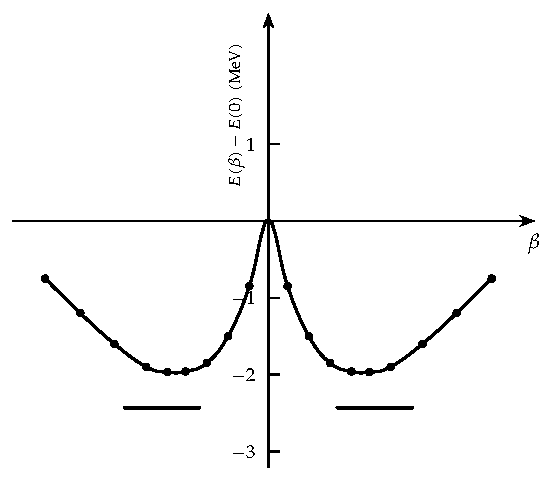
\includegraphics[width=0.6\linewidth]{pictures/7_1}
\par\end{centering}
\centering{}\caption{\label{fig:7_1_Sm152=007ED3=005408=0080FD}作为形变函数的结合能（针对 $\ce{^{152}Sm}$）。极小值之外的横线为自洽计算的解（引自
\cite{DMP66}）。}
\end{figure}

\noindent\textbf{(b) 采用 Skyrme 力的计算}\footnote{利用第 5.6.1.2 节讨论的 Negele 力也进行了类似的计算\cite{NR77}。}。我们在第
5.6.2 节中看到，带有密度依赖 Skyrme 力的 HF 理论能够重现球形核的基态性质。因此它们也被应用于形变情况\cite{Va73}。正如第
7.4 节所讨论的，没有先验的理由对$\Gamma$和$\Delta$的计算采用相同的力。因此，第一步是使用纯配对力 (4.140)
来计算$\Delta$。在时间反演不变的情况下，我们再次发现（如同在对-四极模型中）正则基与$h$为对角矩阵的 HF 基一致。因此，在迭代的每一步中对角化$h$就足够了。与普通
HF 计算唯一的区别在于，在计算密度$\rho,\tau,\boldsymbol{J}$时，我们必须考虑配对能和占据几率$v^{2}_{k}$。代替式
(5.84)，例如我们得到：

\begin{equation}
\rho(\boldsymbol{r})=\sum^{\infty}_{ist}v^{2}_{i}|\varphi_{i}(\boldsymbol{r},s,t)|^{2},\label{eq:skyrme_density_with_pairing}
\end{equation}

其中

\begin{equation}
v^{2}_{i}=\frac{1}{2}\left(1-\frac{\epsilon_{i}-\lambda}{\sqrt{(\epsilon_{i}-\lambda)^{2}+\Delta^{2}}}\right).\label{eq:vi2_skyrme_bcs}
\end{equation}

在此$\lambda$同样由粒子数条件确定。原则上，$\Delta$应当由能隙方程 (6.60) 确定。Vautherin 采取了相反的途径，采用从实验中选取的固定能隙$\Delta$，并利用式
(6.60) 计算了相应的力常数。与球形核 HF 计算的巨大差异在于，在形变核中微分方程 (5.100) 在径向坐标$r$与角度$\theta,\phi$之间不再是可分离的。它现在是一个偏微分方程。Vautherin
通过在各向异性谐振子基中进行对角化求解了该方程。只有矩阵元是在坐标空间中通过高斯积分计算的。轴对称性允许将其分解为具有良好量子数$\Omega$的子空间。尽管如此，这些计算仍然需要巨大的计算工作量\footnote{关于坐标空间中形变 HF 方程的求解，参见 \cite{HN77}。}。

计算结果显示出与实验结合能和半径令人满意的符合。特别地，人们能够重现形变重核测得的四极矩和十六极矩\cite{FQV73}。

\noindent\textbf{(c) 完全 HFB 计算}。正如我们在第 6 章中所见，配对关联不仅取决于有效配对力的性质，还取决于单粒子能级密度。因此，自洽场和配对场由同一种力导出的完全
HFB 计算，仅在 HF 场产生合理的单粒子谱时才具有物理意义。正如第 5 章所讨论的，进行这项任务需要密度依赖的有效力。另一方面，由于现有版本的
Skyrme 力的$\delta$-力性质，它们不适用于完全的 HFB 计算。因此，Gogny \cite{Go73,Go75b,DGG75,DG80}
引入了一种带有有限力程部分的新型密度依赖相互作用（参见第 4.4.4 节）。这种力的高斯形式允许在谐振子基中快速计算矩阵元\cite{Go75a}。

在推导 HFB 方程时，迄今为止我们尚未采用密度依赖力。仿照第 5.6 节，在此时我们必须将能量计算为密度$\rho$和$\kappa$的泛函{[}我们使用式
(E.19) 中定义的约定$\mathrm{Tr}_{1}$和$\mathrm{Tr}_{2}${]}：

\begin{equation}
E'(\rho,\kappa)=\langle\Phi|T+V(\rho)-\lambda\hat{N}|\Phi\rangle=\mathrm{Tr}\,(t-\lambda)\rho+\frac{1}{2}\mathrm{Tr}_{1}\mathrm{Tr}_{1}\rho\bar{v}\rho+\frac{1}{4}\mathrm{Tr}_{2}\mathrm{Tr}_{2}\kappa^{*}\bar{v}\kappa,\label{eq:energy_functional_hfb_density_dep}
\end{equation}

并从变分原理导出 HFB 方程。这通过使用超矩阵$\mathcal{R}$ (7.27) 最容易实现。我们将$(i<k)$的$\rho_{ii},\rho_{ik},\rho^{*}_{ik},\kappa_{ik},\kappa^{*}_{ik}$作为独立变量，并通过
Lagrange 参数矩阵施加关系 (7.28) 作为附加条件（该过程也可以用来推导第 5 章中的普通 HF 方程）：

\begin{equation}
\delta\left(E'(\rho,\kappa)-\mathrm{Tr}(\Lambda(\mathcal{R}^{2}-\mathcal{R}))\right)=0.\label{eq:variational_principle_lagrange_R}
\end{equation}

我们求得：

\begin{equation}
\delta E'=\mathrm{Tr}(\mathcal{H}\cdot\delta\mathcal{R})\label{eq:delta_E_prime}
\end{equation}

其中

\begin{equation}
\delta\mathcal{R}=\begin{pmatrix}\delta\rho & \delta\kappa\\
-\delta\kappa^{*} & -\delta\rho^{*}
\end{pmatrix},\qquad\mathcal{H}=\begin{pmatrix}h & \Delta\\
-\Delta^{*} & -h^{*}
\end{pmatrix}\label{eq:delta_R_supermatrix}
\end{equation}

且

\begin{equation}
h_{ik}=\frac{\delta E'}{\delta\rho_{ki}},\qquad\Delta_{ik}=\frac{\delta E'}{\delta\kappa^{*}_{ik}},\label{eq:hik_deltaik_derivatives}
\end{equation}

在与密度无关力的情况下与式 (7.41) 一致。从式 (7.76) 得到：

\begin{equation}
\mathrm{Tr}((\mathcal{H}-\Lambda\mathcal{R}-\mathcal{R}\Lambda+\Lambda)\delta\mathcal{R})=0.\label{eq:tr_lambda_R}
\end{equation}

由于$\delta\mathcal{R}$是独立变分，这等价于：

\begin{equation}
\mathcal{H}=\Lambda\mathcal{R}+\mathcal{R}\Lambda-\Lambda.\label{eq:H_lambda_R_relation}
\end{equation}

通过条件$\mathcal{R}^{2}=\mathcal{R}$消去$\Lambda$，结果为：

\begin{equation}
[\mathcal{H},\mathcal{R}]=0.\label{eq:H_R_commutator_zero}
\end{equation}

这正是式 (7.43)。它等价于式 (7.36)，并且可以按照求解 HFB 方程 (7.42) 的相同方法求解。然而，在相互作用$v(1,2)$依赖于$\rho$的情况下，我们得到对自洽场$\Gamma$有贡献的额外项。从式
(7.75) 和 (7.79) 可以看出，它们具有如下形式：

\begin{equation}
\frac{1}{4}\frac{\partial}{\partial\rho_{ki}}\mathrm{Tr}_{2}\mathrm{Tr}_{2}(\kappa^{*}\bar{v}[\rho]\kappa).\label{eq:rearrangement_term_pairing}
\end{equation}

通过以合适的方式调节力参数（表 4.4），Gogny 能够重现球形核以及形变核的性质。特别地，他得到了正确的形变与能隙参数（参见表
7.1）。

\begin{table}[H]
\begin{centering}
\caption{\label{tab:7_1_=007ED3=005408=0080FD=007535=008377=0056DB=006781=0077E9=0080FD=009699=006BD4=008F83}结合能
$E$、电荷四极矩 $Q$ 以及质子和中子的能隙参数 $\Delta$ 的实验值与计算值比较（引自 \cite{Go75b}）}
\par\end{centering}
\centering{}%
\begin{tabular}{ccccccccc}
\hline 
核素 & $E_{\text{HFB}}$ {[} & $E_{\text{EXP}}$ {[} & $Q_{\text{HFB}}$ {[} & $Q_{\text{EXP}}$ {[} & $\Delta_{p,\text{HFB}}$ {[} & $\Delta_{p,\text{EXP}}$ {[} & $\Delta_{n,\text{HFB}}$ {[} & $\Delta_{n,\text{EXP}}$ {[}\tabularnewline
\hline 
$\ce{^{150}Sm}$ & 1235.8 & 1239.3 & 383 & 367 & 1.24 & 1.43 & 1.13 & 1.13\tabularnewline
$\ce{^{152}Sm}$ & 1249.0 & 1253.1 & 572 & 590 & 1.14 & 1.08 & 1.09 & 1.24\tabularnewline
$\ce{^{166}Er}$ & 1348.1 & 1351.6 & 770 & 770 & 1.10 & 0.97 & 1.02 & 1.00\tabularnewline
$\ce{^{184}W}$ & 1468.2 & 1472.9 & 631 & 627 & 0.90 & 0.86 & 0.86 & 0.73\tabularnewline
\hline 
\end{tabular}
\end{table}

结合能仍应当针对转动对称性和粒子数破缺所引起的赝贡献进行修正（参见第 11 章）。这些修正可以达到 5 MeV 的数量级\cite{FQV73}。

总结这些结果，我们发现带有密度依赖力的 HFB 理论能够在元素周期表的整个范围内重现球形核与形变核的所有基本基态性质。在下一节中，我们将看到如何将该理论推广到裂变过程能量面的微观计算。

\section{约束Hartree-Fock理论\label{sec:=007EA6=00675FHartree-Fock=007406=008BBA}}

无约束的 HF 和 HFB 计算仅给出能量面上的一个点，即局部极小值。我们通常也对能量面上的其它点感兴趣：我们可以施加某些附加条件，并寻求能量在由它们定义的超曲面上的极小值。有时我们希望将能量面计算为一个（或若干个）集体参数$q$的函数，例如四极或十六极形变。正如我们在第
1 章中所看到的，这是导出集体 Hamilton 量（用于描述集体振动或裂变过程）的第一步。我们将在第 10 章结合生成坐标法更详细地讨论这一点。

在所有这些情况下，我们都对在某个单粒子算符$\hat{Q}$具有固定期望值的约束下使总能量极小化的波函数$|\Phi(q)\rangle$感兴趣：

\begin{equation}
q=\langle\Phi|\hat{Q}|\Phi\rangle.\label{eq:constraint_expectation_q}
\end{equation}

求解该问题的最简单方法是将条件 (7.84) 带有 Lagrange 乘符$\lambda$加到 Hamilton 量$H$中，并求下式的极小值：

\begin{equation}
\langle H'\rangle=\langle H\rangle-\lambda\langle\hat{Q}\rangle.\label{eq:linear_constraint_H_prime}
\end{equation}

在该问题求解之后，$\lambda$由条件 (7.84) 确定。该方法也称为线性约束变分。它对应于考察处于合适地使其发生形变的外场$\hat{Q}$中的多体体系。

该方法已经应用于 BCS 理论（第 6.3.2 节）中，以获得具有粒子数正确期望值的波函数。与式 (6.41) 类似，我们发现 Lagrange
乘符$\lambda$是能量$E=\langle\Phi|H|\Phi\rangle$对$q$的导数：

\begin{equation}
\lambda=\frac{\mathrm{d}E}{\mathrm{d}q}.\label{eq:lambda_dE_dq}
\end{equation}

正如我们从图 7.2 所看到的，线性约束的方法意味着我们必须在点$q=q_{0}$处作能量面$E(q)$的切线，并将该切线作为旋转了角度$\alpha$（其中$\tan\alpha=\lambda$）的新坐标系的$x$轴。新坐标系中的$y$轴对应于$\langle H'\rangle$。对$\langle H'\rangle$进行无约束变分给出了旋转坐标系中能量面的极值。

显然，只要函数$E(q)$具有正的二阶导数，该过程就可以有效工作。在曲线向下凹的情况下——例如在裂变路径上的鞍点附近或在回弯区（图
3.4）——该方法将不再有效。在这些情况下，旋转坐标系中的能量在点$q_{1}$处具有极大值，它永远不会是 HF 方程的稳定解。

\begin{figure}[H]
\begin{centering}
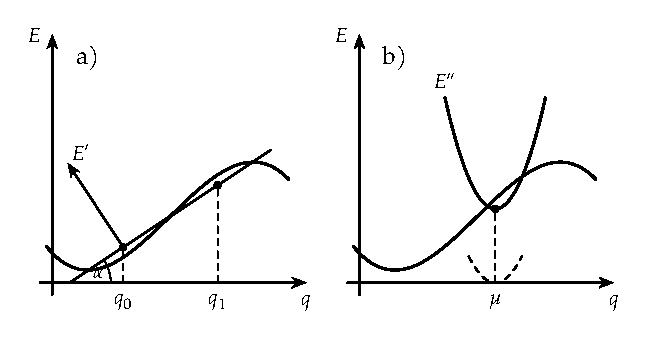
\includegraphics[width=0.7\linewidth]{pictures/7_2}
\par\end{centering}
\centering{}\caption{\label{fig:7_2_=0080FD=0091CF=009762=007EA6=00675F=00793A=00610F=0056FE}示意性能量面，展示了线性约束（a）与二次约束（b）的方法。}
\end{figure}

我们还认识到，在拐点附近总是存在若干个具有平行切线的点（即具有相同的$\lambda$，但具有不同的$q$值），也就是说，$q$不再是
Lagrange 参数的单值函数（参见图 3.6）。

存在若干种避免该问题并寻找能量面上此类点的波函数的方法：

(i) 梯度法（如第 7.3 节所讨论）允许我们沿着垂直于对$\hat{Q}$的梯度的最速下降线前进。因此，对于每个$q$值，我们都能找到相应的能量极小值。

(ii) 二次约束法\cite{GLW70,FQK73}采用对函数

\begin{equation}
E''=\langle H\rangle+\frac{1}{2}C(\langle\hat{Q}\rangle-\mu)^{2}\label{eq:quadratic_constraint_function}
\end{equation}

的无约束变分。如图 7.2b 所示，这里我们在能量面上添加了一条对称轴为$q=\mu$的抛物线。它产生了一个在$\mu$附近具有极值的新曲面$E''$。如果其宽度充分小（$C>|\mathrm{d}^{2}E/\mathrm{d}q^{2}|$），这始终是一个真正的极小值。$E''$的变分给出：

\begin{equation}
\delta\langle H\rangle-C(\mu-\langle\hat{Q}\rangle)\delta\langle\hat{Q}\rangle=0.\label{eq:variation_E_double_prime}
\end{equation}

这意味着二次约束等价于具有$\lambda=C(\mu-\langle\hat{Q}\rangle)$的线性约束。在两种情况下，我们得到相同的能量面。对于作为$\langle\hat{Q}\rangle$的函数的任何约束，这都是正确的。采用二次约束，$\lambda$的有效值在迭代过程中自动改变。

(iii) 第三种方法\cite{BW71}使用线性约束，但在迭代的每一步中改变$\lambda$的值，使得条件 (7.84)
得到满足。该方法应用于带有粒子数约束的 BCS 计算中。然而，它需要在每一步进行额外的迭代。

约束 Hartree-Fock 理论（CHF）已被用于计算原子核在基态附近的能量面\cite{BKS67,CLF73,CS73,FQK73,GG78}以及裂变过程\cite{FQV74,KCS74,BFV74}。

在后一种情况下，通常必须面对应当使用何种约束算符$\hat{Q}$的问题。容易证明，通过使用合适的约束算符$\hat{Q}_{\Phi}$进行
CHF 计算，我们可以找到任何乘积波函数$|\Phi\rangle$。我们只需使用双准粒子部分$Q^{20}$被定义为$H^{20}$的倍数的算符。随后我们得到：

\begin{equation}
H^{20}-\lambda Q^{20}=0,\label{eq:chf_q20_condition}
\end{equation}

也就是说，$|\Phi\rangle$作为相应 CHF 方程的解。当然，这对于计算$|\Phi\rangle$没有太大的实用价值，但它表明存在种类繁多的约束算符，它们产生相同的波函数，仅在它们的$Q^{11}$-矩阵元上有所不同。

\begin{figure}[H]
\begin{centering}
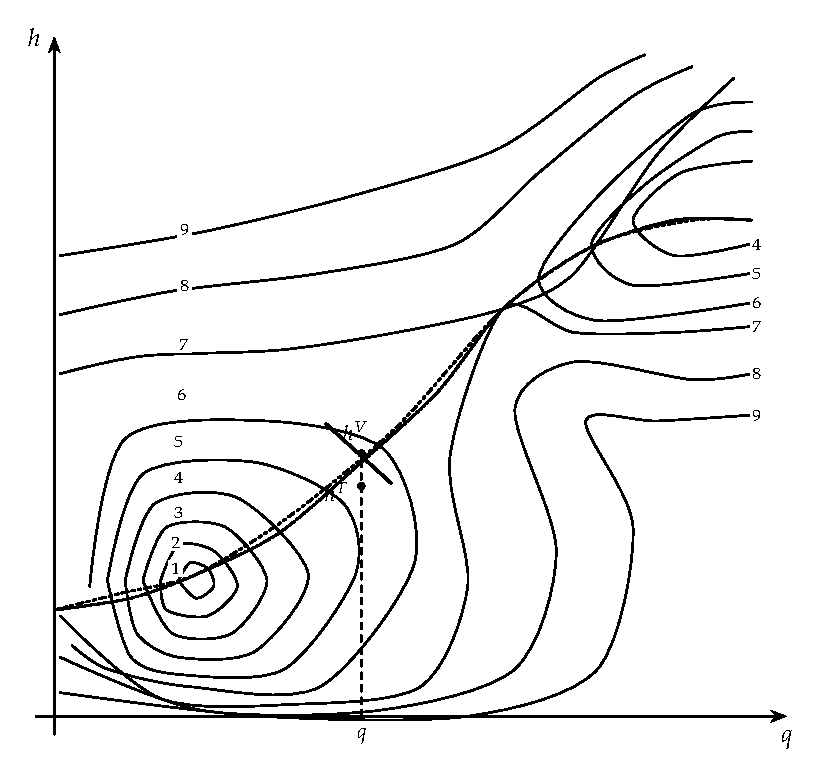
\includegraphics[width=0.65\linewidth]{pictures/7_3}
\par\end{centering}
\centering{}\caption{\label{fig:7_3_qh=0080FD=0091CF=009762=0088C2=0053D8=008C37}$(q,h)$
平面内的能量面示例，表明仅对 $q$ 加约束并不能精确跟踪裂变谷（引自 \cite{FQK73}）。}
\end{figure}

另一方面，对一种形变的约束（例如四极形变$q=\langle\Phi|Q_{20}|\Phi\rangle$）并不意味着另一种形变（例如十六极形变$h=\langle\Phi|Q_{40}|\Phi\rangle$）保持不变。这在图
7.3 中示意性地给出。只要我们对$q$使用约束，我们就沿着线$h^{1}(q)=\langle\Phi(q)|Q_{40}|\Phi(q)\rangle$行进。它连接了每个等势面上的垂直切点，因为对于恒定的$q$，$E$必须对所有其它自由度达到极小，这意味着特别是$\mathrm{d}E/\mathrm{d}h|_{q=\text{const}}=0$。这条线$h^{1}(q)$通常与裂变谷底不同，后者对应于最速下降线$h^{0}(q)$。两条线都穿过能量面的驻点，例如基态极小值或鞍点。如果裂变谷平行于$q$轴，这两条线非常接近；但如果裂变谷平行于$h$轴，它们可能会发生相当剧烈的偏离。尽管如此，与液滴模型和
Strutinsky 式计算（参见第 2.9 节）相比，我们认识到 CHF 计算的巨大优势：在 CHF 计算中，我们只需追踪单参数曲线，就能获得在许多情况下与裂变谷底非常接近的波函数，而在其它方法中我们必须计算多维能量面。

在 CHF 计算中，我们当然应该优化约束算符的选择。在第 10 章中，我们将研究实现这一目标的方法。

\begin{figure}[H]
\begin{centering}
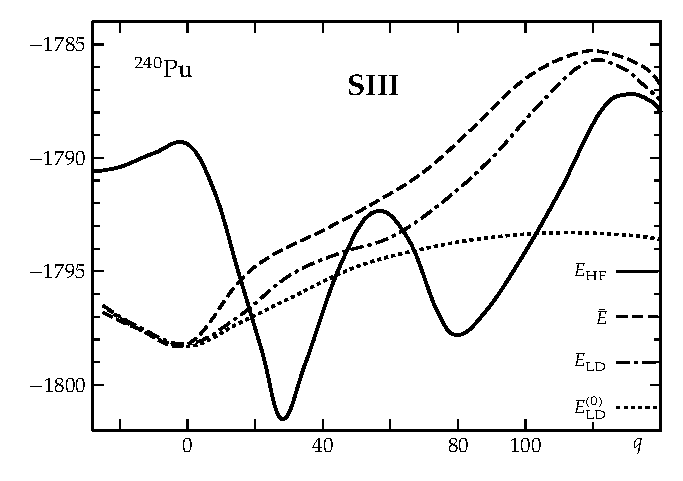
\includegraphics[width=0.65\linewidth]{pictures/7_4}
\par\end{centering}
\centering{}\caption{\label{fig:7_4_Pu240=005F62=0053D8=0080FD=0066F2=007EBF}利用 Skyrme
III 相互作用作为质量四极矩 $q$ 的函数计算出的 $\ce{^{240}Pu}$ 形变能曲线。详细说明见正文（引自 \cite{BQ75a}）。}
\end{figure}

图 7.4 展示了利用带有质量四极矩$q$约束的 Skyrme 力计算得到的原子核$\ce{^{240}Pu}$的形变能（实线\cite{FQV74}）。对关联通过简单的对力来考虑，其常数$G$选为与核表面积成正比。该计算重现了基态极小值和第二极小值。势垒的高度在定量上与实验数据不符，但我们必须记住，在计算中保持了轴对称性和空间反射宇称，而有迹象表明实际的裂变路径在内鞍点破坏了轴对称性，在外界鞍点破坏了空间反射宇称。

为了将这些结果与液滴模型计算进行比较，计算了 Strutinski 平均的 HF 能量（虚线）并显示在图 7.4 中。它显示出微小的起伏波动。然而，这些起伏并不是由壳效应引起的，它们也存在于对应于相同形变$q$和$h$的液滴能量中（点划线），因为该曲线与侧谷相交。裂变谷底的液滴能量（点线）是非常平滑的。

图 7.5 显示了同一原子核在不同形变下的质子密度分布。

\begin{figure}[H]
\begin{centering}
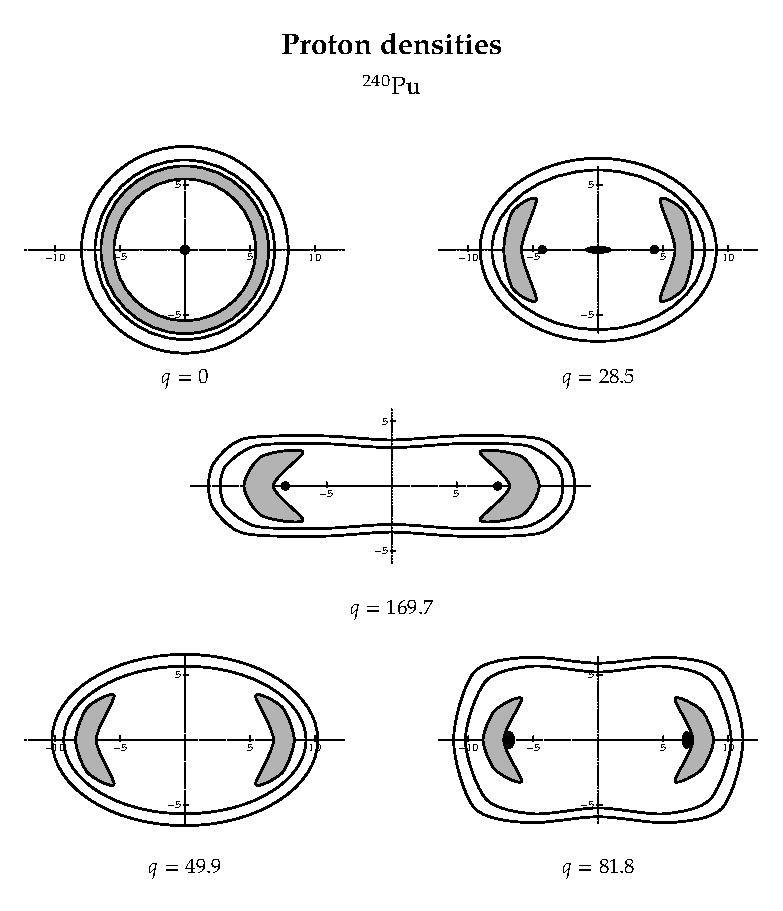
\includegraphics[width=0.7\linewidth]{pictures/7_5}
\par\end{centering}
\centering{}\caption{\label{fig:7_5_Pu240=008D28=005B50=005BC6=005EA6=005206=005E03}$\ce{^{240}Pu}$
在不同形变 $q=\langle Q_{20}\rangle$ 下的质子密度分布（引自 \cite{FQV74}）。}
\end{figure}

若干作者\cite{FS76,BSV76}指出，如果允许波函数$|\Phi\rangle$在空间中扩展得非常远，带有具有无界能谱约束算符（例如当$r\to\infty$时发散的$Q\sim r^{2}Y_{20}$）的此类
CHF 计算可能会给出非常虚假的解。然而，CHF 方法的所有实际应用都是在有限组态空间中进行的，这确保了波函数$|\Phi\rangle$定域在原子核的区域内。

因此，在组态空间的选择上，我们受到来自两方面的限制：为了获得结合能的收敛，通常需要大的组态空间；但另一方面，我们不应该能够表象上述的虚假解。看来迄今为止进行的
CHF 计算都保持在这些限制之内。

保持核波函数定域的另一种可能途径是引入第二个约束\cite{GL77}：

\begin{equation}
\hat{H}'=\hat{H}-\lambda\hat{Q}+\mu\hat{Q}^{2}.\label{eq:second_constraint_operator}
\end{equation}

Lagrange 参数$\mu$将允许我们改变波函数中的$\langle\Delta\hat{Q}^{2}\rangle$涨落。

\section{转动系下的HFB理论\label{sec:=008F6C=0052A8=007CFB=004E0B=007684HFB=007406=008BBA}}

在第 3 章中，我们在纯单粒子壳模型的框架内讨论了 cranking 模型。它为我们提供了微观计算转动惯量的可能性。显而易见如何将该理论推广到自洽多体体系：我们必须在角动量算符$J_{x}$具有确定期望值的附加条件下，对多体
Hamilton 量$H$的期望值进行变分。这给出了方程（亦参见第 11.4 节）：

\begin{equation}
\delta\langle\Phi|H-\omega J_{x}|\Phi\rangle=0.\label{eq:cranking_variation_scc}
\end{equation}

cranking 频率$\omega$依赖于角动量$I$，并由下式确定：

\begin{equation}
\langle\Phi_{\omega}|J_{x}|\Phi_{\omega}\rangle=\sqrt{I(I+1)}.\label{eq:cranking_frequency_condition}
\end{equation}

在第 11 章中我们将看到，该问题的解$|\Phi_{\omega(I)}\rangle$必须被理解为内禀波函数，在实验室坐标系中通过投影到好的角动量上可以从中获得$\boldsymbol{J}^{2}$的本征函数。

在 HFB 理论中，我们将变分函数的集合$|\Phi\rangle$限制为 HFB 类型的广义乘积函数，这样我们便面对一个带有约束的
HFB 问题。类似于单粒子情况下的 cranking 模型，该方法被称为自洽 cranking 模型（self-consistent
cranking model, SCC）。在上一节中，我们已经非常详细地讨论了约束 HF 方法的问题。在回弯区（参见第 3 章以及
\cite{CMR75}），式 (7.91) 的解对应于在恒定$\omega$下能量面上的鞍点。因此，我们必须应用梯度法或二次约束以在回折分支上获得解。

与迄今为止所讨论的 HFB 理论的应用不同，波函数$|\Phi\rangle$的时间反演对称性被算符$\omega J_{x}$破坏。因此，我们无法先验地知道正则基中的共轭态，从而必须在转动系中求解完全的
HFB 问题\cite{RBM70}，即：

\begin{equation}
\begin{pmatrix}h-\omega j_{x} & \Delta\\
-\Delta^{*} & -h^{*}+\omega j^{*}_{x}
\end{pmatrix}\begin{pmatrix}U_{k}\\
V_{k}
\end{pmatrix}=\begin{pmatrix}U_{k}\\
V_{k}
\end{pmatrix}E_{k}.\label{eq:cranking_hfb_equation}
\end{equation}

利用被 cranking Hamilton 量所保持的对称性$\mathrm{e}^{\mathrm{i}\pi j_{x}}$，矩阵$\rho,\kappa,\Gamma$以及$\Delta$具有形式
(7.67)。由于时间反演对称性$T$被破坏，代替式 (7.69)，我们有：

\begin{equation}
\rho_{2}\ne\rho^{*}_{1};\qquad\Gamma_{2}\ne\Gamma^{*}_{1};\qquad D_{2}\ne D^{*}_{1};\qquad\kappa^{\dagger}_{1}\ne\kappa_{1};\qquad\Delta^{\dagger}_{1}\ne\Delta_{1}.\label{eq:time_reversal_broken_relations}
\end{equation}

因此，密度和势具有时间偶部分和时间奇部分，例如：

\begin{equation}
\rho^{(+)}=\rho_{1}+\rho^{*}_{2};\qquad\rho^{(-)}=\rho_{1}-\rho^{*}_{2}.\label{eq:rho_time_even_odd}
\end{equation}

在$\omega=0$时二重简并的准粒子能量$E_{k}$（参见第 2.8 节），在有限的 cranking 频率下发生分裂（图
7.8d），并且不再由公式 (7.51) 给出。然而，根据 Bloch-Messiah 定理 (7.7)，存在一个正则基，可以通过对角化密度$\rho$找到。正如我们从式
(7.50) 可以看出的，在此基下的占据几率$v^{2}_{k}$由下式给出：

\begin{equation}
v^{2}_{k}=\frac{1}{2}\left[1-\frac{\epsilon_{k}-\omega j_{x_{k}}}{\sqrt{(\epsilon_{k}-\omega j_{x_{k}})^{2}+\Delta^{2}_{k\bar{k}}}}\right],\label{eq:vk2_cranking_canonical}
\end{equation}

其中$\epsilon_{k}=\frac{1}{2}(h_{kk}+h_{\bar{k}\bar{k}})$且$j_{x_{k}}=\frac{1}{2}(j_{x_{kk}}+j_{x_{\bar{k}\bar{k}}})$。

这表明在正则基下的对角矩阵元$h_{kk},j_{x_{kk}},h_{\bar{k}\bar{k}},j_{x_{\bar{k}\bar{k}}}$以及$\Delta_{k\bar{k}}$是决定占据几率的关键量。矩阵$h,j_{x}$和$\Delta$本身在此基下通常不是对角的。人们还会注意到，具有较大正矩阵元$j_{x_{k}}$的能级比较大负值的能级具有更大的占据几率。

自洽 cranking 模型对于描述高自旋区发现的异常现象非常有用\footnote{最近，cranking 模型用于描述带交叉的有效性已成为讨论的对象 \cite{Ha76,Ha77,MG78,GSF78b,CDS78}。}，这些现象在第
3 章中曾予以讨论。它足够普遍，能够涵盖种类繁多的物理效应。为了说明这一点，我们将讨论原子核$\ce{^{164}Er}$的某些效应，该核在近几年中在实验上得到了非常深入的研究\cite{LCS76,KSM78}。人们已经发现了延伸至相当高自旋值的若干条转动带（参见图
7.6）。

\begin{figure}[H]
\begin{centering}
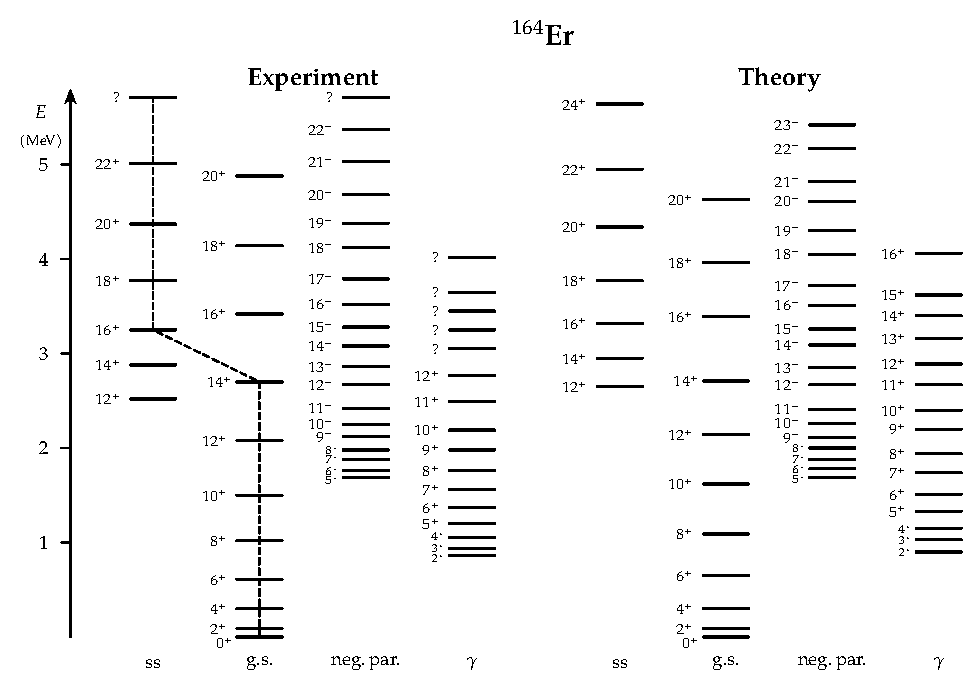
\includegraphics[width=0.7\linewidth]{pictures/7_6}
\par\end{centering}
\centering{}\caption{\label{fig:7_6_Er164=008F6C=0052A8=005E26=0080FD=008C31}$\ce{^{164}Er}$
中的转动带能谱。除基态带（gs）外，还展示了由对准的 $i_{13/2}$ 中子对构成的 Stephens-Simon 带（ss）、负宇称带和
$\gamma$ 带 \cite{KSM78}。Yrast 线（虚线所示）沿着每个 $I$ 值的最低能级。右侧给出了 SCC
方法的理论计算结果 \cite{MSR76,EMR80a,EMR80b}。}
\end{figure}

方程 (7.91) 的变分给出了每个$I$值的最低能量。根据定义，这就是 yrast 线（图 7.6 中的虚线）。正如我们所见，它仅在$I=14$之前跟随基态带。在$I=14$与$I=16$之间，出现了一个带交叉，也就是说，如果我们沿着
yrast 线就会发生回弯（参见图 7.7）。相交叉的带具有带有两个对准的$i_{13/2}$中子的双准粒子带的结构。因此，yrast
线改变了它的性质：它在$I=14$之前跟随基态带，而对于所有$I\geqslant16$的值对应于对准带。在自洽 cranking
模型内沿着 yrast 线的能级计算展现出以下特征：

\begin{figure}[H]
\begin{centering}
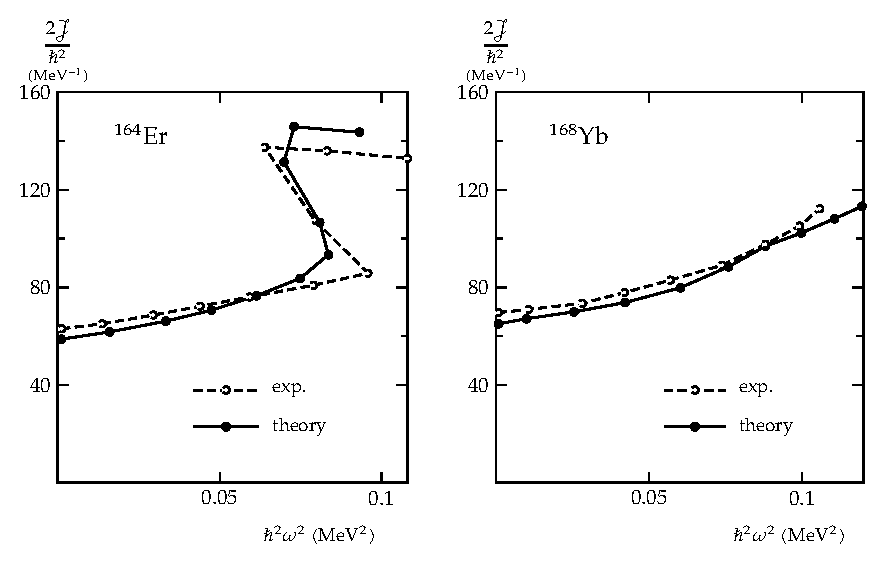
\includegraphics[width=0.7\linewidth]{pictures/7_7}
\par\end{centering}
\centering{}\caption{\label{fig:7_7_Er164_Yb168=0056DE=005F2F=0056FE}原子核 $\ce{^{164}Er}$
和 $\ce{^{168}Yb}$ 的回弯图。虚线代表实验数据，实线为 SCC 理论的计算结果 \cite{MSR76}。转动惯量
$\mathcal{J}$ 和角频率 $\omega$ 的定义见式 (3.3)。}
\end{figure}

\noindent\textbf{(i) 伸展效应（The Stretching Effect）}代表转动过程中核形变可能发生的变化。它由自洽势$\Gamma$所描述，该势依赖于密度，因而依赖于
cranking 频率。图 7.8a 显示了在$\ce{^{164}Er}$的 SCC 计算中发现的有效核形变$\beta$和$\gamma$。在此自旋区域内形变$\beta$的改变相当小。对于许多良好形变的稀土核也是如此。另一方面，$\gamma$-形变增加至$\gamma\sim10^{\circ}$，但这强烈依赖于具体原子核，其它原子核对于$\gamma$-形变可能相当刚硬。

\noindent\textbf{(ii) Coriolis 反配对效应（The Coriolis Antipairing Effect,
CAP）}意味着核内的对关联被 Coriolis 力削弱。在第 6 章中我们看到，对关联主要来源于相反自旋的核子对（Cooper 对），由于它们具有大的空间重叠而感受到强相互作用。由于
Coriolis 力在相反方向作用于两个角动量上（图 7.9），我们应当预期至少会出现部分对准以及相应的配对能$\Delta$随自旋增加而降低。这在计算中得到了证实（图
7.8b），并解释了低自旋值下转动惯量的适度增加。正如磁场中的超导体一样，在某一临界角动量下，我们发现了向正常流体态的相变。这种核
Meissner 效应由 Mottelson 和 Valatin \cite{MV60} 所预言，并在许多计算中（例如 \cite{CV66,RBM70,Wa70a,Ku72,Fr76}）在各不相同的自旋值下被发现。

\begin{figure}[H]
\begin{centering}
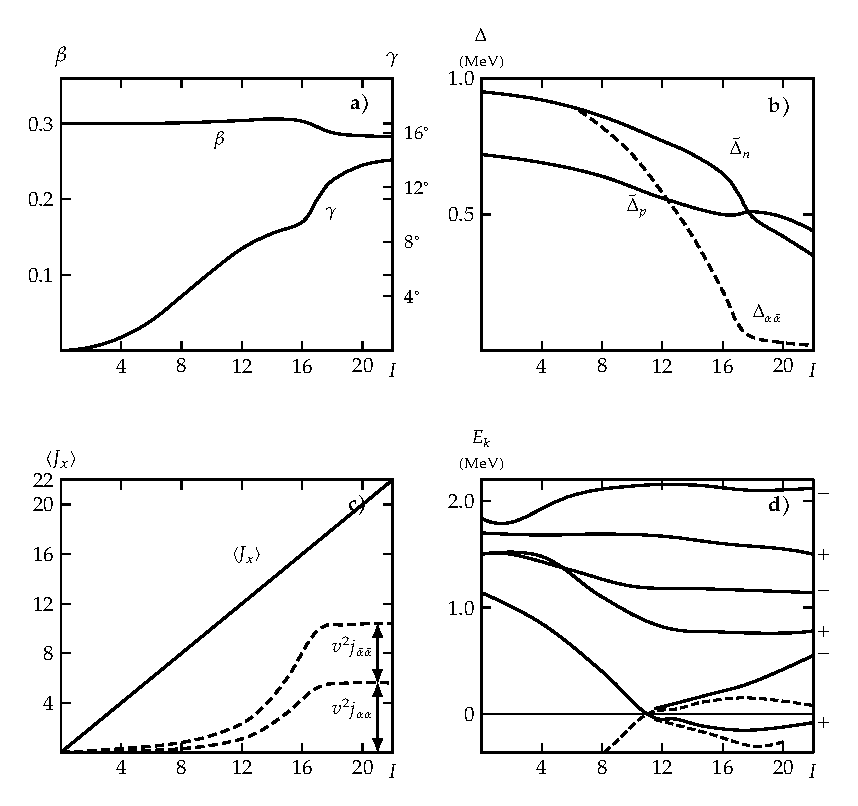
\includegraphics[width=0.7\linewidth]{pictures/7_8}
\par\end{centering}
\centering{}\caption{\label{fig:7_8_Er164=007406=008BBA=0053C2=006570=0053D8=005316}$\ce{^{164}Er}$
计算得到的形变参数（a）、能隙参数（b）、角动量期望值 $J_{x}$（c）以及转动系中的准粒子能量 $E_{k}$（d）随角动量的变化（引自
\cite{MSR76}）。$\beta$ 形变的值归一化为 $I=0$ 时的 0.3。部分（b）显示了质子和中子在正则基下的平均能隙参数
$\tilde{\Delta}_{p}$ 与 $\tilde{\Delta}_{n}$ {[}式 (7.97){]} 以及对准对的能隙参数
$\Delta_{\alpha\bar{\alpha}}$（虚线）。更详细的说明见正文。}
\end{figure}

\begin{figure}[H]
\begin{centering}
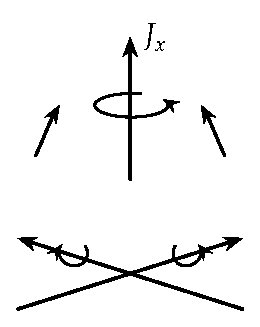
\includegraphics[width=0.45\linewidth]{pictures/7_9}
\par\end{centering}
\centering{}\caption{\label{fig:7_9_CAP=006548=005E94=00793A=00610F=0056FE}Coriolis 反配对效应（CAP）的示意图。}
\end{figure}

回弯现象曾被认为是由这种相变引起的\cite{KS73}。然而，允许一对或几对核子发生解耦过程的更现实计算表明，配对能隙$\Delta$在回弯区域并没有完全消失（图
7.8b，在$I=12$和$I=16$之间）。由于对准过程，它仅仅是减小了。这对应于向具有相应阻塞效应的双准粒子带的转变（参见第
6.3.4 节）。在图 7.8b 中，我们展示了平均能隙：

\begin{equation}
\tilde{\Delta}=\frac{1}{M'}\sum^{M'}_{k>0}\Delta_{k\bar{k}}.\label{eq:average_gap_def}
\end{equation}

（$M'=M/2$是组态空间中$k>0$的能级数。）即使对于在原始基下具有常数配对矩阵元$\Delta$的常数配对力，在正则基下的所有矩阵元$\Delta_{k\bar{k}}$也并不都相等。特别地，对准对的矩阵元$\Delta_{\alpha\bar{\alpha}}$趋向于零（图
7.8b 中的虚线）。这种效应对于仅作用于$I=0$对的纯配对力表现得最为显著（参见第 4.4.7 节）。极高自旋态的现实计算仍有待进行。然而，模型计算和实验数据\cite{BSC75}表明，剩余的对关联仍然存在，有时甚至维持到相当高的自旋值（$I\sim40\text{--}50\hbar$）。

\noindent\textbf{(iii) 对准过程（Alignment Processes）}（Stephens-Simon
效应，\cite{SS72a}；参见第 3.2 节）。由于 HFB 波函数$|\Phi\rangle$是最普遍的单粒子态的乘积（具有相应的占据几率），它们不仅可以代表基态带，还可以代表部分或完全对准的双准粒子带的态。因此，它们是在微观上研究此类解耦过程的合适工具。然而显然，我们必须允许轴对称性的破坏以描述此类对准态，它们是许多不同$\Omega$值的混合（参见第
3.3 节）。这在 cranking 计算中不成问题，因为 Coriolis 项$\omega j_{x}$无论如何都破坏了这种对称性。

对准的程度由两粒子在正则基下的矩阵元$j_{x_{\alpha\alpha}}$和$j_{x_{\bar{\alpha}\bar{\alpha}}}$来量度。图
7.8c 展示了这些数值{[}乘以相应的占据几率 (7.96)，后者事实上非常接近于 1{]}以及$J_{x}$的总期望值。人们注意到，在回弯区，$J_{x}$总增量的大部分以上来自于这一对粒子。其余粒子的贡献减少，这对应于该区域内角频率$\omega$的减小。对于更高的自旋值，对准对的贡献相当稳定在$5.8+4.8\simeq10.6$，而一个完全对准的$i_{13/2}$对将给出$13/2+11/2=12$。

\noindent (iv) 最后，图 7.8d 展示了转动系中的某些准粒子能量 $E_{k}$\}，它们是式 (7.93) 的本征值随角动量的变化。它们不再是二重简并的，而在时间反演不变的情况下是二重简并的。在大角动量下，可能会发生这些能量之一趋于零并变为负值的情况。由于配对势在该区域并未消失，该现象被称为无能隙超导（gapless
superconductivity）\footnote{在金属超导体中也出现类似的现象 \cite{AG61}。}
\cite{GLS67,Gr74,CMR75}。然而，这并不意味着存在更低能量的激发态，因为偶体系中的激发能始终是两个准粒子能量之和。我们看到，对于式
(7.93) 的每个本征值$E_{k}$，我们也有一个本征值$-E_{k}$（虚线）。这些“非物理”本征值之一在回弯区变为正值。然而，我们不被允许选取这个正本征值，因为（正如在第
7.3.2 节中所讨论的）这将对应于向奇粒子数体系波函数的转变。我们还在图 7.8d 中（通过细线）标出了带交叉现象，该现象与回弯区从基态带向双准粒子带的转变相关联。

在稀土区的所有原子核中都发现了类似的特征\footnote{关于 SCC 理论在轻核中的应用，参见 \cite{PM76,NS78,Zi78}。}。然而，在回弯图上存在显著的差异（参见图
7.7），因为此类图对能谱能级间距的微小改变非常敏感。在许多情况下，此类对准过程确实发生而并不伴随回弯现象。正如模型计算\cite{CMR75}所示，是否发生回弯取决于底层的单粒子能级密度以及两个相交叉带之间的剩余相互作用：弱相互作用和低能级密度给出突然对准，因而导致回弯。在其它情况（例如$\ce{^{168}Yb}$）下，我们具有平滑的对准过程而没有回弯（亦参见第
122 页的脚注）。

此类计算最初由慕尼黑小组\cite{BMR73}在有限组态空间中利用对-四极相互作用完成。与此同时，该理论已通过粒子数投影得到了改进\cite{DBM73,FDG76}。正如第
11 章所讨论的，这在对关联经历剧烈改变的区域中似乎是必要的。定量上与实验的符合通过此类计算得到了一定程度的改善，但上面讨论的定性图像没有任何改变。将四极对力包含在内也是如此\cite{WF78a}。

人们还使用了更现实的力，如在有限空间中从 Reid 软芯势导出的$G$-矩阵\cite{GVS76,Go76a}或 Skyrme
类型的相互作用\cite{FMR79}。发现了定性上相似的结果。

在第 7.3.2 节中我们看到，我们不仅可以将 HFB 类型的函数$|\Phi\rangle$用于偶核基态以及沿着 yrast 线的态，还可以用于偶核和奇核中的所有类型的准粒子态。因此，在
SCC 方法中，我们还可以描述奇核中的转动带以及偶核中的一般双准粒子带。特别地，我们可以研究所有类型的对准过程。

第 11 章中对 cranking 模型更基本的推导表明，我们应当使用附加条件：

\begin{equation}
\langle J_{x}\rangle=\sqrt{I(I+1)-\langle J^{2}_{z}\rangle}\label{eq:cranking_condition_exact_projection}
\end{equation}

代替式 (7.92)。对于良好近似下轴对称的偶核基态带，$\langle J^{2}_{z}\rangle$相当小。在这些情况下，式
(7.98) 等价于式 (7.92)。利用这一附加条件计算了奇核中严重受扰动的转动带\cite{RMB74,FDB77}，并发现与实验能谱很好地符合（图
3.11）。特别地，在该模型中无需对 Coriolis 相互作用进行任何衰减因子修正\cite{RM74,Ri77}。

图 7.6 给出了具有负宇称的双准粒子带的例子。在这里一个中子位于$i_{13/2}$壳层，另一个中子位于负宇称壳层。我们再次观察到一个$i_{13/2}$中子的对准过程，这引起该带较低能级具有小的能级间距。由于宇称选择定则，相应的波函数自动与基态正交。这在引起回弯现象的所谓“第二”带的计算中是不同的。它是一个激发带，在回弯点处其特征从对准的双准粒子带转变为基态带。该带具有与
yrast 带相同的对称性。因此，我们必须施加额外的约束，即其波函数与 yrast 带的相应波函数正交\cite{EMR80a}。

图 7.6 还展示了一条$\gamma$-带。正如我们将在下一章看到的，此类集体振动无法由纯乘积波函数来描述。然而，这并不意味着建立在此类振动上的转动带不能用
cranking 模型进行研究。我们只需对$|\Phi\rangle$采用更复杂结构的波函数（例如下一章讨论的 TDA 或 RPA
波函数；\cite{Ho68,CMR75,Ma77a,ERM78,ERM80b}）。

让我们以如下总结性评述结束本章：HFB 理论是一种在推广的静态单粒子图像中包含尽可能多的关联的方法。因此，它定义了两个自洽确定的场{[}即序参量（参见第
11 章）{]}：用于$ph$-关联的平均势$\Gamma$，以及用于$pp$-关联的配对势$\Delta$。在这一理论框架内，我们能够重现球形核与形变核的基态性质。它还可以用于描述具有广义乘积类型波函数的激发态，例如纯准粒子激发或良好形变核中的转动态。在后一种情况下，必须对平均角动量施加约束。然而，我们应该记住，形变波函数必须被理解为内禀波函数，在实验室坐标系中通过投影到角动量本征态上可以从中获得波函数（参见第
11.4 节）。

此外，HFB 理论可用于为处理进一步关联的更复杂方法提供最优基。这将在后续章节中进行。



\chapter{简谐振动\label{chap:=007B80=008C10=00632F=0052A8}}

\section{导论\label{sec:8.1_=005BFC=008BBA}}

在对原子核性质进行微观描述时，到目前为止我们仅仅使用了静态的独立粒子模型。我们已经看到，通过合理地定义粒子或准粒子，并采用有效相互作用，我们能够在此类图像下解释许多原子核基态的基本性质。原子核激发能谱对于理解核结构同样极为重要。如果我们在核壳模型内，或在更为精细的独立粒子模型（例如
Hartree-Fock 或 Hartree-Fock-Bogoliubov）内对这些能谱进行分析，便会发现一系列激发态能够非常令人满意地用诸如粒子-空穴（ph）激发或双准粒子激发来解释。然而，也存在大量激发态，其特征根本无法在壳模型激发的框架内予以重现——尽管通过引入涉及对称性破缺的精巧方法，我们已经能够将核子间的重要关联考虑在内。

例如，若我们将讨论局限于球对称双幻核，如 $^{16}\mathrm{O}$、$^{40}\mathrm{Ca}$ 或 $^{208}\mathrm{Pb}$，则根据核壳模型的简谐振子近似，最低的激发能级应当位于约
$1\hbar\omega_{0}$ 处。对于 $^{16}\mathrm{O}$，实验测得的 $1p$ 壳与 $2s\text{-}1d$
壳之间的壳间距大约为 $11.5\,\text{MeV}$。然而，在 $^{16}\mathrm{O}$ 的能谱中，除其他态之外，我们在
$6.14\,\text{MeV}$ 处观察到一个 $(J^{\pi}=3^{-},\,T=0)$ 态；而在约 $22\,\text{MeV}$
处，观察到一个宽约 $5\,\text{MeV}$ 的共振峰，通常称为巨偶极共振（见\ref{fig:8_1}），其量子数为 $J^{\pi}=1^{-},\,T=1$。

\begin{figure}[H]
\begin{centering}
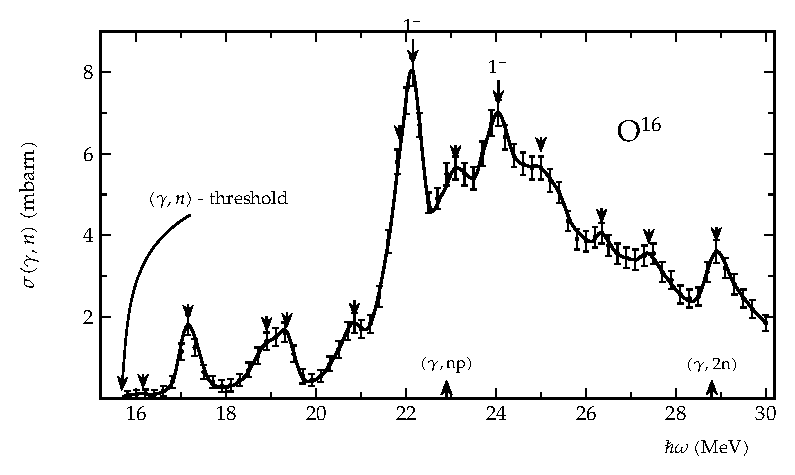
\includegraphics[width=0.8\textwidth]{pictures/8_1}
\par\end{centering}
\caption{\label{fig:8_1}$(\gamma,n)$ 反应截面随 $\gamma$ 能量的变化（引自 \cite{BCH64}）。}
\end{figure}

可以证明（见第 8.3.3 节），该共振主要涉及 $1\hbar\omega$ 激发。因此，纯壳模型同样无法解释巨偶极共振如此之高的能量。

事实表明，只有假定核内大量核子发生了相干协同参与，才能对这些激发做出解释。我们目前对“相干”的理解，还只能借助原子核的经典液滴方法（第
1 章）来表述：人们认为许多核子以类似于核液滴形状振动的方式共同参与运动。在下文中，我们将了解量子力学意义上的相干究竟意味着什么。此外，这类集体激发通常满足以下判据：
\begin{enumerate}
\item 它们的电磁跃迁几率具有集体增强强度，比单粒子跃迁大一到两个数量级（参见第 2.7.2 节）。
\item 它们在元素周期表不同区域各原子核的能谱中展现出极强的规律性。例如，巨偶极共振在整个周期表中均已被观测到，其激发能随质量数缓慢变化［$\propto80A^{-1/3\div-1/6}$，见式
(1.44)］。
\end{enumerate}
球形核以及变形核的能谱中都包含大量满足这些判据的态。我们将把讨论局限于普遍方法上，这些方法在剩余相互作用［式 (2.35)］

\begin{equation}
V_{R}=\frac{1}{4}\sum_{kk',ll'}\bar{v}_{kk'll'}a^{\dagger}_{k}a^{\dagger}_{k'}a_{l'}a_{l}-V_{\text{HF}}\label{eq:tda_residual_interaction}
\end{equation}

的框架下，能够同时解释高激发（通常为共振）以及低激发（通常为束缚态）的集体振动。正如式 (\ref{eq:tda_residual_interaction})
所示，在下文中我们将主要采用 Hartree-Fock 单粒子图像，因为这能使讨论更为简捷。然而必须强调的是，在以下各节中介绍的所有方法，只要采用
HFB 准粒子（参见第 7 章）替代粒子，都可以直接进行推广。在某些特定情况下，我们也会对此做明确展示。

在第 8.2 节中，我们基于无关联的 HF 基态研究 ph 对之间的相互作用（Tamm-Dancoff 近似，TDA）。在第 8.3
节中，介绍不同类型的集体激发。基态关联将在第 8.4 节中于随机相位近似（RPA）框架下加以考虑，并证明 TDA 方法固有的若干困难可以通过这种途径得以解决。在第
8.5 节中，我们将展示如何利用线性响应理论的形式体系推导出相同的方程，以及在处理密度依赖相互作用时会呈现哪些特征。在第 8.6 节中，给出该理论的一些数值应用。求和规则是提取此类共振普适性质、并阐明
RPA-Hamiltonian 量的量子力学本征态与表面振动经典图像之间联系的有力手段，它们将在第 8.7 节中展开讨论。最后，第
8.8 节与第 8.9 节专门讨论 RPA 的特殊推广，如粒子-粒子 RPA 以及准粒子 RPA。

\section{Tamm-Dancoff 方法\label{sec:8.2_Tamm-Dancoff=0065B9=006CD5}\label{sec:8.2_Tamm-Dancoff=008FD1=004F3C}}

\subsection{Tamm-Dancoff 久期方程\label{subsec:8.2.1_Tamm-Dancoff=004E45=00671F=0065B9=007A0B}}

若我们将壳模型势用 $A$ 个核子填充至某个费米能级，如\ref{fig:8_2} 所示，那么所有零、单、双、三、四、$\dots$、$N$
粒子壳模型激发就构成了一组完备的正交基，可用于展开基态 $|0\rangle$ 或激发态 $|\nu\rangle$ 的真实多核子波函数。此时，Schrödinger
方程的精确解可以通过在全壳模型空间中对 $H$ 进行对角化来获得，或者等价地，通过对以下展开系数进行变分来求解。［在下文中，我们约定指标
$m,n$（$i,j$）分别限制在费米面以上（以下）。］

\begin{equation}
|0\rangle=C^{0}_{0}|\text{HF}\rangle+\sum_{mi}C^{0}_{mi}a^{\dagger}_{m}a_{i}|\text{HF}\rangle+\frac{1}{4}\sum_{mnij}C^{0}_{mn,ij}a^{\dagger}_{m}a^{\dagger}_{n}a_{j}a_{i}|\text{HF}\rangle+\cdots\label{eq:tda_expansion_ground}
\end{equation}

\begin{equation}
|\nu\rangle=C^{\nu}_{0}|\text{HF}\rangle+\sum_{mi}C^{\nu}_{mi}a^{\dagger}_{m}a_{i}|\text{HF}\rangle+\frac{1}{4}\sum_{mnij}C^{\nu}_{mn,ij}a^{\dagger}_{m}a^{\dagger}_{n}a_{j}a_{i}|\text{HF}\rangle+\cdots\label{eq:tda_expansion_excited}
\end{equation}

在理想情况下，行列式 $|\text{HF}\rangle$ 应当由填充 Hartree-Fock 势的 $N$ 个最低单粒子能级给出。然而，后者通常用唯象单粒子势来近似。算符
$a^{\dagger}_{m}a_{i}$ 因而湮灭一个费米能级 $\epsilon_{F}$ 之下的粒子（产生一个空穴），并在
$\epsilon_{F}$ 之上产生一个粒子。因此，它被称为粒子-空穴产生算符（\ref{fig:8_2}）。

\begin{figure}[H]
\begin{centering}
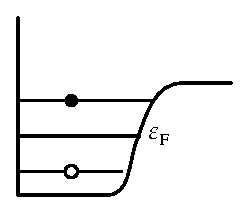
\includegraphics[width=0.5\textwidth]{pictures/8_2}
\par\end{centering}
\caption{\label{fig:8_2}壳模型中的粒子-空穴（ph）激发示意图。}
\end{figure}

在全壳模型空间中精确对角化 $H$ 是一项无法完成的任务。然而，让我们假设在式 (\ref{eq:tda_expansion_excited})
的激发态 $|\nu\rangle$ 展开中，仅保留至 1 粒子-1 空穴（1p-1h）激发是合理的。稍后我们将看到，对于某些类型的状态，这确实是一个极佳的近似。先验地看，也有充分理由说明为何如此：$1\hbar\omega$
粒子-空穴激发子集是能量最低的壳模型组态，因此对于负宇称的低激发态应当极为重要。由电磁场 $F=\sum_{pp'}F_{pp'}a^{\dagger}_{p}a_{p'}$
激发的态的跃迁几率正比于 $|\langle0|F|\nu\rangle|^{2}$，因此这些态被认为具有主导的粒子-空穴贡献。由此我们有理由期望，若在展开式
(\ref{eq:tda_expansion_ground}) 和 (\ref{eq:tda_expansion_excited})
中仅保留以下项：

\begin{equation}
|0\rangle=C^{0}_{0}|\text{HF}\rangle+\sum_{mi}C^{0}_{mi}a^{\dagger}_{m}a_{i}|\text{HF}\rangle\label{eq:tda_ansatz_ground}
\end{equation}

则至少对某一类状态能获得相当不错的近似。由于 $\langle\text{HF}|Ha^{\dagger}_{m}a_{i}|\text{HF}\rangle=0$［式
(5.35)］，我们看到拟设 (\ref{eq:tda_ansatz_ground}) 意味着基态保持为一个行列式，而对于激发态，只需保留

\begin{equation}
|\nu\rangle=\sum_{mi}C^{\nu}_{mi}a^{\dagger}_{m}a_{i}|\text{HF}\rangle\label{eq:tda_ansatz_excited}
\end{equation}

就足够了。这种做法的主要缺点在于：仅在激发态中考虑了关联，而基态保持未关联。稍后我们将看到如何在基态中也建立起关联。

由于 Hamilton 算符与总角动量算符 $\boldsymbol{J}$ 对易，且在很多情况下也与总同位旋算符 $\boldsymbol{T}$
对易，我们理应采用 Clebsch-Gordan 耦合形式的拟设 (\ref{eq:tda_ansatz_excited})［见式
(2.46)］。为了不破坏公式的简明性，除非绝对必要，下文中我们将略去耦合角动量指标。

将式 (\ref{eq:tda_ansatz_excited}) 作为变分拟设，结合

\begin{equation}
\delta\frac{\langle\nu|H|\nu\rangle}{\langle\nu|\nu\rangle}=0\label{eq:tda_variational_principle}
\end{equation}

我们如通常那样得到用于确定本征值和展开系数的久期方程：

\begin{equation}
\sum_{nj}\langle\text{HF}|a^{\dagger}_{i}a_{m}Ha^{\dagger}_{n}a_{j}|\text{HF}\rangle C^{\nu}_{nj}=E_{\nu}C^{\nu}_{mi}\label{eq:tda_secular_matrix}
\end{equation}

利用式 (5.35)，我们可以将式 (\ref{eq:tda_secular_matrix}) 改写为更为便利的形式：

\begin{equation}
\langle\text{HF}|a^{\dagger}_{i}a_{m}[H,a^{\dagger}_{n}a_{j}]|\text{HF}\rangle=(E_{\nu}-E_{\text{HF}})C^{\nu}_{mi}\label{eq:tda_secular_double_commutator}
\end{equation}

式 (\ref{eq:tda_secular_double_commutator}) 中的对易子可利用式 (5.25) 和 (5.26)
容易地求出：

\begin{align}
[H,a^{\dagger}_{n}a_{j}] & =(\epsilon_{n}-\epsilon_{j})a^{\dagger}_{n}a_{j}+\frac{1}{2}\sum_{kl}\left(\bar{v}_{knlj}a^{\dagger}_{n}a^{\dagger}_{k}a_{l}-\bar{v}_{kllj}a^{\dagger}_{k}a^{\dagger}_{l}a_{j}\right)\nonumber \\
 & \quad+\frac{1}{4}\sum_{klm'n'}\bar{v}_{klm'n'}[a^{\dagger}_{k}a^{\dagger}_{l}a_{n'}a_{m'},a^{\dagger}_{n}a_{j}]\label{eq:tda_commutator_h_ph}
\end{align}

利用 Hartree-Fock 单粒子能 $\epsilon$ 的定义式 (5.37) 以及计算场算符基态期望值的规则（附录 C），我们最终得到所谓的
Tamm-Dancoff 方程：

\begin{equation}
(\epsilon_{m}-\epsilon_{i})C^{\nu}_{mi}+\sum_{nj}\bar{v}_{mjin}C^{\nu}_{nj}=E^{\text{TDA}}C^{\nu}_{mi}\label{eq:tda_secular_equation}
\end{equation}

［通过适当选择能量零点，已令 $E_{\text{HF}}=0$，而 $E^{\text{TDA}}$ 是 Tamm-Dancoff
近似（TDA）下 $|\nu\rangle$ 的激发能］。

用图形来表示相互作用的矩阵元通常非常有用：

\begin{equation}
v_{mjin}=\int\mathrm{d}\xi_{1}\mathrm{d}\xi_{2}\phi^{*}_{m}(\xi_{1})\phi^{*}_{j}(\xi_{2})v(\xi_{1},\xi_{2})\phi_{i}(\xi_{1})\phi_{n}(\xi_{2})\label{eq:tda_interaction_integral}
\end{equation}

变量 $\xi$ 象征性地代表全部坐标，且积分包含了对自旋和同位旋的求和。费曼图的绘制规则在许多专著中均有阐述［AGD 63, Ma
67b］；由于我们并不打算将图解法作为一门独立工具来介绍，而仅仅是用作已解析推导内容的直观图示，在此我们不作过多细节铺陈，仅给出绘制约定。波浪线代表
$v$，带箭头的实线代表单粒子波函数（箭头向上代表粒子；箭头向下代表空穴），根据它们的坐标连接到波浪线的相互作用点 1 和 2 上。此外，我们通常约定：在公式
(\ref{eq:tda_interaction_integral}) 中位于相互作用 $v$ 右侧的线指向相互作用点，而左侧的线则背离相互作用点。基于这些约定，$v_{mjin}$
可以用图形展示，如\ref{fig:8_3} 所示。

\begin{figure}[H]
\begin{centering}
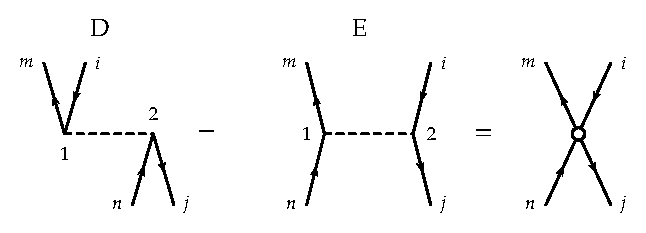
\includegraphics[width=0.75\textwidth]{pictures/8_3}
\par\end{centering}
\caption{\label{fig:8_3}矩阵元 $v_{mjin}$ 与 $v_{mjni}$ 的图形表示。}
\end{figure}

若我们设想垂直于波浪线存在一条时间轴，则在直接项 D 中，一个粒子-空穴对 $nj$ 被湮灭，同时产生了另一个对 $mi$；而在交换项
E 中，粒子-空穴对 $nj$ 散射为一个新的对 $mi$。若将波浪线想象为 $\pi$ 介子，“直接”和“交换”的含义就更加直观了：过程
D 是一个对产生和对湮灭过程（正如电动力学中波浪线代表光子、空穴代表正电子、粒子代表电子那样）；而图 E 则代表在粒子-空穴对之间交换了一个
$\pi$ 介子的过程。通常，直接项与交换项可合并为一个图（Feynman 图），如\ref{fig:8_3} 所示。

\subsection{示意模型\label{subsec:8.2.2_=00793A=00610F=006A21=00578B}\label{subsec:8.2.2_=0096C6=004F53=006027=007684=005224=00636E}}

Tamm-Dancoff 方程的解一般无法在全粒子-空穴空间中求得，因为这是一项极其庞大的数值任务。因此，在大多数情况下仅保留一个“模型空间”，其中包含费米能级
$\epsilon_{F}$ 上下的若干能级。这些计算也常被称为组态混合或壳模型计算。在进入更多细节之前，我们希望在一个极其简明的模型中研究
TDA 方程解的定性特征，在该模型中我们可以得到解析形式的解。

\subsubsection{采用可分离相互作用求解 TDA 方程}

若假定剩余相互作用的矩阵元在粒子-空穴指标上是可分离的（参见第 4.4.7 节及 \cite{BB59,BET61}）：

\begin{equation}
\bar{v}_{mjin}=\chi D_{mi}D^{*}_{nj}\label{eq:tda_separable_force}
\end{equation}

则式 (\ref{eq:tda_secular_equation}) 的求解大为简化。进一步假定 $D_{mi}$ 为某一多极算符（例如四极算符）的矩阵元：

\begin{equation}
D_{mi}=\langle m|r^{2}Y_{2\mu}|i\rangle\label{eq:tda_multipole_element}
\end{equation}

多极阶数自然与粒子-空穴对 $(m,i)$ 耦合到的角动量相一致。矩阵元 (\ref{eq:tda_separable_force})
固然未按严格要求进行反对称化。然而事实证明，交换项很小，将其忽略是一个很好的近似［BK 68, Ma 74］。通常，剩余相互作用对
$T=0$ 态是吸引的（它们的能量被向下推移，例如 $^{16}\mathrm{O}$ 中的 $3^{-},\,T=0$ 态），而对
$T=1$ 态则是排斥的［BB 59］。因此，我们必须选取：

\begin{align}
\chi & <0\quad(\text{对 }T=0),\nonumber \\
\chi & >0\quad(\text{对 }T=1).\label{eq:tda_coupling_sign}
\end{align}

有充分理由表明，相互作用拟设 (\ref{eq:tda_separable_force}) 并不像表面看起来那样简陋，但在此我们不打算深入探讨可分离力的深层物理（见第
4.4.7 节）。相反，我们希望将式 (\ref{eq:tda_separable_force}) 视作一种极为便利的简化，使我们能够探究
TDA 解的定性特征。

基于拟设 (\ref{eq:tda_separable_force})，久期方程 (\ref{eq:tda_secular_equation})
具有如下形式：

\begin{equation}
(E^{\text{TDA}}-\epsilon_{m}+\epsilon_{i})C_{mi}=\chi D_{mi}\sum_{nj}D^{*}_{nj}C_{nj}\label{eq:tda_separable_secular}
\end{equation}

态 $|\nu\rangle$ 当然应当归一化，根据式 (\ref{eq:tda_ansatz_excited})，我们有：

\begin{equation}
\sum_{mi}|C_{mi}|^{2}=1\label{eq:tda_normalization}
\end{equation}

由于 $\sum_{nj}D^{*}_{nj}C_{nj}=\text{const.}$，我们可以从式 (\ref{eq:tda_separable_secular})
中解出展开系数 $C_{mi}$：

\begin{equation}
C_{mi}=N\frac{D_{mi}}{E^{\text{TDA}}-\epsilon_{m}+\epsilon_{i}},\quad N=\left[\sum_{mi}\frac{|D_{mi}|^{2}}{(E^{\text{TDA}}-\epsilon_{m}+\epsilon_{i})^{2}}\right]^{-1/2}\label{eq:tda_separable_coefficients}
\end{equation}

将式 (\ref{eq:tda_separable_secular}) 乘以 $D^{*}_{mi}(E^{\text{TDA}}-\epsilon_{m}+\epsilon_{i})^{-1}$
并对 $m,i$ 求和，便得到决定激发能 $E^{\text{TDA}}$ 的本征值方程：

\begin{equation}
\frac{1}{\chi}=\sum_{mi}\frac{|D_{mi}|^{2}}{E^{\text{TDA}}-\epsilon_{m}+\epsilon_{i}}\label{eq:tda_dispersion_relation}
\end{equation}

我们可以通过绘制右端项随 $E^{\text{TDA}}$ 变化的函数曲线，图形化地求解式 (\ref{eq:tda_dispersion_relation})。由此，本征值就是该函数与水平直线
$1/\chi$ 的交点。所有解都被夹在原始壳模型激发能 $\epsilon_{mi}=\epsilon_{m}-\epsilon_{i}$
之间，唯独有一个解被大幅推高（若 $1/\chi>0$）或大幅拉低（若 $1/\chi<0$）。有限粒子-空穴空间的假设似乎介入了这一论证，但我们必须记住，确定宇称的
ph 壳模型激发聚集为相隔约 $2\hbar\omega_{0}$ 的若干能级簇。因此，\ref{fig:8_4} 仅仅展示了其中一个能级簇。

\begin{figure}[H]
\begin{centering}
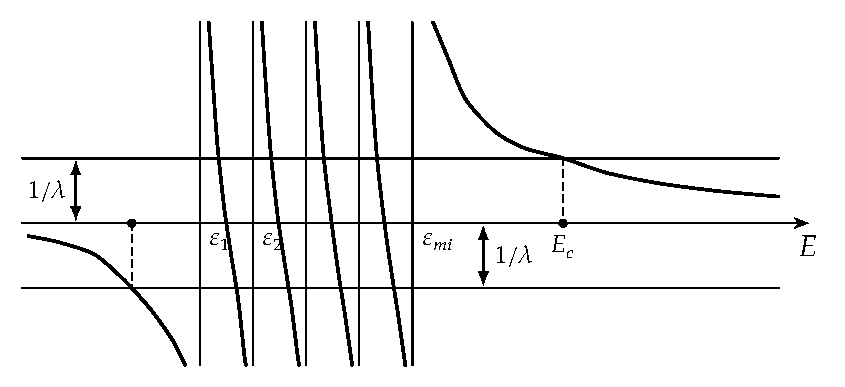
\includegraphics[width=0.75\textwidth]{pictures/8_4}
\par\end{centering}
\caption{\label{fig:8_4}方程 (\ref{eq:tda_dispersion_relation}) 的图解。}
\end{figure}

这一个被显著拉低（$T=0$）或大幅推高（$T=1$）的激发态，是由剩余相互作用的所有矩阵元相干叠加而成的态。这里“相干”的意思是所有矩阵元都以相同的符号做出贡献。这类态的典型例子是在
$^{16}\mathrm{O}$、$^{40}\mathrm{Ca}$ 和 $^{208}\mathrm{Pb}$ 中出现在低激发能处的首个八极态（$T=0$），以及我们稍后将讨论的巨偶极共振（$T=1$）。

\subsubsection{简并情形}

若我们将所有 $\epsilon_{mi}$ 设为相同的值 $\epsilon$，则由式 (\ref{eq:tda_separable_coefficients})
和 (\ref{eq:tda_dispersion_relation}) 容易得出：

\begin{align}
C_{mi} & =\left(\sum_{nj}|D_{nj}|^{2}\right)^{-1/2}D_{mi},\nonumber \\
E^{\text{TDA}} & =\epsilon+\chi\sum_{mi}|D_{mi}|^{2},\label{eq:tda_degenerate_solution}
\end{align}

这意味着集体态被相互作用的所有对角元素之和推高（或拉低）。

这种简并情形可以在例如球形谐振子势（不含自旋-轨道耦合项）中只考虑一个粒子主壳和另一个空穴主壳时实现。在真实原子核中情况不会如此极端，但其本质特征仍很可能得以保持。

对于简并情形，可以通过研究不同激发对总跃迁几率的分配来展现该移动态的集体性。对于集体态，我们有

\begin{equation}
|\text{coll}\rangle=\left(\sum_{mi}|D_{mi}|^{2}\right)^{-1/2}\sum_{mi}D_{mi}a^{\dagger}_{m}a_{i}|\text{HF}\rangle\label{eq:tda_collective_state}
\end{equation}

因此对于跃迁几率，我们得到

\begin{equation}
|\langle\text{coll}|D|0\rangle|^{2}=\left|\left(\sum_{mi}|D_{mi}|^{2}\right)^{-1/2}\sum_{mi}|D_{mi}|^{2}\right|^{2}=\sum_{mi}|D_{mi}|^{2}\label{eq:tda_collective_transition_prob}
\end{equation}

展开系数相干叠加［此处跃迁算符 $D=\sum_{kk'}D_{kk'}a^{\dagger}_{k}a_{k'}$ 应当与可分离相互作用中的算符一致］。

对于所谓的求和规则（参见第 8.7 节），我们得到：

\begin{equation}
\sum_{\nu}|\langle\nu|D|0\rangle|^{2}=\sum_{mi}|\langle mi|D|0\rangle|^{2}=\sum_{mi}|D_{mi}|^{2}\label{eq:tda_sum_rule_exhaustion}
\end{equation}

在此我们将 ph 空间中的完备基 $|\nu\rangle$ 替换为完备基 $|mi\rangle$。对比式 (\ref{eq:tda_collective_transition_prob})
可以看出，总求和规则被集体态完全耗尽。

这意味着在简并情形下，从基态到任何非集体态的跃迁几率均为零。另一方面，到集体态的跃迁几率［式 (\ref{eq:tda_collective_transition_prob})］获得了极大的增强。由此，我们对\ref{fig:8_1}
中所示的强 $1^{-}$ 共振得到了定性解释。

\subsection{粒子-粒子（空穴-空穴）Tamm-Dancoff 方法\label{subsec:8.2.3_=007C92=005B50-=007C92=005B50=00FF08=007A7A=007A74-=007A7A=007A74=00FF09Tamm-Dancoff=0065B9=006CD5}}

正如我们在双幻核情形所看到的，超越 Hartree-Fock 的最简单关联只能通过打破 HF 核心、并将一个核子从费米能级之下提升到其之上来考虑。在远离双幻核时，即通过向下一个开壳填充核子，另一种截然不同的关联就显得至关重要。由于幻核被认为是相当稳定的实体，价核子之间的关联似乎单独决定了关于这些原子核已知的各种实验事实。涵盖从
$^{16}\mathrm{O}$ 到 $^{40}\mathrm{Ca}$ 的 $s\text{-}d$ 壳核也许是此类“开壳”核中研究得最透彻的范例。为了处理这类原子核，人们发展了一整套理论，最广为人知的名称是壳模型组态混合计算。该理论的许多要素可在
de-Shalit 和 Talmi 的专著［ST 63］中找到，而该理论框架下最先进的计算是由 Oak Ridge 组［HMW 71］以及
Whitehead［Wh 72］完成的。在本节中，我们只想讨论这类原子核最简单的情形，即仅偏离闭壳两个粒子，从而填入两个核子或移去两个核子（产生两个空穴）。根据上面的阐述并类比于
ph 情形，我们尝试如下变分拟设（pp-TDA 方法）：

\begin{equation}
|1,A+2\rangle=\sum_{m<n}C^{1}_{mn}a^{\dagger}_{m}a^{\dagger}_{n}|\text{HF}\rangle\label{eq:pptda_ansatz}
\end{equation}

系数 $C_{mn}$ 假定是反对称的，即 $C_{mn}=-C_{nm}$。完全类比于 ph-TDA 情形，我们得到 pp-TDA
久期方程：

\begin{equation}
(E^{\text{TDA}}_{1}-\epsilon_{m}-\epsilon_{n})C^{1}_{mn}=\sum_{m'<n'}\bar{v}_{mnm'n'}C^{1}_{m'n'}\label{eq:pptda_secular_equation}
\end{equation}

这是一个线性 Hermitian 本征值问题。本征矢必须满足归一化与完备性关系（$n<m,\,n'<m'$）：

\begin{equation}
\sum_{m<n}C^{1*}_{mn}C^{1'}_{mn}=\delta_{11'}\label{eq:pptda_orthonormality}
\end{equation}

\begin{equation}
\sum_{1}C^{1}_{mn}C^{1*}_{m'n'}=\delta_{mm'}\delta_{nn'}\label{eq:pptda_closure}
\end{equation}

正如所指出的，原则上求和遍及所有 $>\epsilon_{F}$ 的能级，因此包含了束缚态与连续态。由于这通常会导致矩阵规模超出当今计算机的能力，我们通常在受限子空间中工作，只考虑费米能级之上的一个或两个主壳。为了补偿未包含能级的影响，必须采用适当“重整化”的有效相互作用（参见第
4.3.2 节）。对于 hh-TDA 情形，方程与式 (\ref{eq:pptda_secular_equation}) 完全相同，只需将粒子指标
$(m,n)$ 替换为空穴指标 $(i,j)$，并将单粒子能的符号取反。pp（hh）方程的解可以展现出与 ph 情形相似的特征。例如，我们也可以得到低激发的集体态，通常称为配对振动（参见第
8.3.5 节）。由于定性讨论与 ph 情形非常相似，我们在此不再赘述。（关于铅同位素区域的计算，可参见例如［HK 72, MT 73］及相关文献）。

\section{集体模式的一般考量\label{sec:8.3_=0096C6=004F53=006A21=005F0F=007684=004E00=00822C=008003=0091CF}}

\subsection{量子力学中的振动\label{subsec:8.3.1_=0091CF=005B50=00529B=005B66=004E2D=007684=00632F=0052A8}}

或许现在是暂时中断我们对 TDA 方法多少有些形式化讨论的合适时机，以便更深入地审视集体态的本质。在第 1 章中，我们将这些态描述为液滴的振动。在量子力学语境下，“振动”一词可能会令人困惑，因为我们实际上处理的仅仅是定态。这种定态的密度
$\rho(\boldsymbol{r})$ 是与时间无关的。这里的对应关系大致类似于在量子力学谐振子问题中谈论振荡。为了得到围绕基态密度
$\rho^{(0)}(\boldsymbol{r})$ 振动的含时密度分布 $\rho(\boldsymbol{r},t)$，我们必须研究包含基态
$|0\rangle$ 以及少量激发态 $|\nu\rangle$ 掺杂的波包：

\begin{equation}
|\Psi(t)\rangle=e^{-\mathrm{i}E_{0}t/\hbar}\left(|0\rangle+\sum_{\nu}c_{\nu}e^{-\mathrm{i}\Omega_{\nu}t}|\nu\rangle\right)\label{eq:coll_wavepacket}
\end{equation}

式中 $\hbar\Omega_{\nu}=E_{\nu}-E_{0}$。在系数 $c_{\nu}$ 的一阶近似下，相应的密度为（参见附录
D）：

\begin{align}
\rho(\boldsymbol{r},t) & =\langle\Psi(t)|\sum_{i}\delta(\boldsymbol{r}-\boldsymbol{r}_{i})|\Psi(t)\rangle\nonumber \\
 & =\rho^{(0)}(\boldsymbol{r})+\delta\rho(\boldsymbol{r},t)\label{eq:coll_density_expansion}
\end{align}

其中

\begin{equation}
\delta\rho(\boldsymbol{r},t)=\sum_{\nu}\left(c_{\nu}e^{-\mathrm{i}\Omega_{\nu}t}\rho^{(\nu)}(\boldsymbol{r})+c^{*}_{\nu}e^{\mathrm{i}\Omega_{\nu}t}\rho^{(\nu)*}(\boldsymbol{r})\right)\label{eq:coll_density_variation}
\end{equation}

对该密度进行 Fourier 分析，便可给出不同激发态的贡献：

\begin{equation}
\rho^{(\nu)}(\boldsymbol{r})=\langle0|\sum_{i}\delta(\boldsymbol{r}-\boldsymbol{r}_{i})|\nu\rangle\label{eq:coll_transition_density}
\end{equation}

这些物理量被称为跃迁密度（transition densities）。

一般而言，我们不仅期望如式 (\ref{eq:coll_density_expansion}) 所示在密度的局域部分出现振荡，而且期望在非局域部分也发生振荡，也就是说，我们对跃迁密度矩阵感兴趣。正如附录
D 中所讨论的，在壳模型基下，它具有如下形式：

\begin{equation}
\rho^{(\nu)}_{kk'}=\langle0|a^{\dagger}_{k'}a_{k}|\nu\rangle\label{eq:coll_transition_density_matrix}
\end{equation}

在 TDA 方法中，这些矩阵元由式 (\ref{eq:tda_ansatz_excited}) 中的系数 $C^{\nu}_{mi}$
给出，即在 TDA 中有：

\begin{equation}
\rho^{(\nu)*}_{mi}=C^{\nu}_{mi}\label{eq:coll_tda_density_matrix}
\end{equation}

根据其各种自由度，原子核可以呈现出许多不同类型的运动模式：原子核可以发生形变、平移或压缩；质子与中子的密度可以同相位或反相位振动；在自旋和同位旋自由度上也可以发生振动；我们还有配对模式以及许多其他模式，在下文中我们只能讨论其中若干最基本的模式。

\subsection{集体模式的分类\label{subsec:8.3.2_=0096C6=004F53=006A21=005F0F=007684=005206=007C7B}}

由于本章讨论的是简谐振动，在下文中我们将更详细地探究其定性性质。为了看清其基本结构，我们将讨论局限于球对称闭壳核，最合适的研究范例是
$^{208}\mathrm{Pb}$。然而，这些考量同样适用于元素周期表中的其他区域。事实上，正如我们在导论中所见，许多此类集体激发展现出相当经典的属性，它们平滑地依赖于质量数。

集体粒子-空穴（ph）振动可以通过相应对算符［Mo 76a, b］

\begin{equation}
(a^{\dagger}a)_{J^{\pi}T}\label{eq:coll_pair_operator}
\end{equation}

的性质来表征。Hamiltonian 量具有若干精确对称性，例如转动不变性、宇称守恒以及电荷守恒，对应着量子数 $J$、$\pi$
和 $T_{z}$。此外，对于轻核和重核，我们还拥有（正如第 2.6.3 节中所讨论的）带有量子数 $T$ 的近似同位旋对称性。由于我们从处于基态（$J^{\pi}=0^{+}$）的球形闭壳核出发，激发的角动量与宇称完全由耦合对
$(a^{\dagger}a)_{J^{\pi}}$ 的相应量子数所决定。对于轻核（$N=Z$，基态 $T=0$），同位旋的情况亦是如此。对于重核，基态的同位旋为
$T_{0}=(N-Z)/2$，它必须与 ph 对的同位旋耦合成总同位旋 $T=T_{0}$ 或 $T=T_{0}+1$\footnote{$T=T_{0}-1$ 仅在质子粒子-中子空穴激发中才可能出现，对应于相邻奇奇核中的状态。}。我们通常根据
ph 对 $a^{\dagger}a$ 的同位旋变化 $\Delta T$ 对激发进行分类。因此，我们有 $\Delta T=0$
或 $\Delta T=1$ 激发；并且 $\Delta T=1$ 的激发并不必然意味着 $T=T_{0}+1$。

除了这些给出例如角分布信息的关于对称性的一般考量之外，我们还希望根据 ph 对

\begin{equation}
a^{\dagger}(\boldsymbol{r},s,\tau)a(\boldsymbol{r}',s',\tau')\label{eq:coll_general_ph_density}
\end{equation}

中的不同自由度，对集体运动进行更为精确的分类：

(a) 首先，存在原子核局域密度 $\rho(\boldsymbol{r})$ 在空间中的振动。由于此类振动的角度依赖性已完全由角动量决定，我们只需考虑不同的径向形状。在此语境下最简单的例子是具有清晰表面的球体表面振动，我们在第
1.4 节中对此进行了非常详尽的讨论。由式 (1.7) 可以发现，对于这种具有清晰表面的表面振动，跃迁密度 (\ref{eq:coll_transition_density})
给出为：

\begin{equation}
\rho^{(\nu)}(\boldsymbol{r})=\begin{cases}
\rho_{0}, & r\text{ 介于 }R_{0}\text{ 与 }R(\theta,\phi)\text{ 之间},\\
0, & \text{其他区域},
\end{cases}\label{eq:coll_sharp_surface_transition_density}
\end{equation}

即核内部的密度保持恒定，整个跃迁全部集中在表面区域。我们也可以设想 $\rho^{(\nu)}(\boldsymbol{r})$
具有其他径向依赖形式，其中内部密度也发生改变。这类激发被称为呼吸模（breathing modes）。

(b) 另一种截然不同的运动类型同样仅涉及空间自由度，即跃迁密度矩阵非局域部分 $\rho^{(\nu)}(\boldsymbol{r},\boldsymbol{r}')$
的振动。一个典型的例子是原子核扭曲模（twist mode），其中原子核的局域密度保持不变，仅仅内禀速度分布发生振荡（参见［HE 77］）。

(c) 同位旋是一个额外的自由度。在此我们必须区分同一原子核内的激发（$\Delta T_{z}=0$）与同位旋翻转过程（$\Delta T_{z}=-1$），后者属于电荷为
$Z+1$、中子数为 $N-1$ 的相邻原子核。在第一种情况下，ph 对可以耦合为 $\Delta T=0$ 或 $\Delta T=1$。因此，对于迄今讨论的所有模式我们都有两种选择：质子与中子同相位振动（$\Delta T=0$，同位旋标量模），或质子与中子反相位振动（$\Delta T=1$，同位旋矢量模）。在固定空间点
$\boldsymbol{r}$ 处，我们最终会观察到电荷分布的振荡，这对应于核内的极化波。$\Delta T_{z}=-1$
的振动情形是类似共振（模拟共振），将在第 8.3.4 节中展开讨论。

(d) 最后，我们还拥有自旋自由度。相应的振动产生自旋波。

迄今给出的不同模式的分类，在很大程度上基于坐标空间中的考量，并强调了其经典方面。然而在真实的有限核中，这些模式并未得到完全纯粹的实现。总是或多或少存在非集体态的剧烈掺杂。因此，采用基于最简形式壳模型——简谐振子——的截然不同的分类方法通常极其有用。

\ref{fig:8_5} 示意性地展示了闭壳核（如 $^{208}\mathrm{Pb}$）的壳层结构。我们具有正负宇称交替的壳层，彼此之间相隔约
$1\hbar\omega_{0}$ 的能量距离。对于闭壳核，费米面恰好位于两个壳层之间，因此我们发现负宇称的 $1\hbar\omega_{0}$
激发 ph 对，正宇称的 $2\hbar\omega_{0}$ 激发，负宇称的 $3\hbar\omega_{0}$ 激发等等。对于处于闭壳之间的原子核，我们此外还在壳层内部拥有
$0\hbar\omega_{0}$ 激发。

\begin{figure}[H]
\begin{centering}
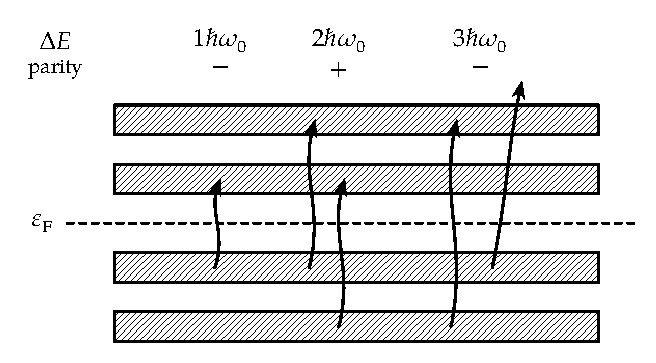
\includegraphics[width=0.75\textwidth]{pictures/8_5}
\par\end{centering}
\caption{\label{fig:8_5}闭壳核中壳层结构与可能出现的 1p-1h 激发示意图。}
\end{figure}

在真实原子核中，简并的振子壳层发生分裂，少数具有“错误”宇称的能级由于自旋-轨道耦合项 $\boldsymbol{l}\cdot\boldsymbol{s}$
的作用向下移入较低的壳层中。这也导致了闭壳核（如 $^{208}\mathrm{Pb}$）中出现正宇称的 $1\hbar\omega_{0}$
激发。但该图像的基本特征在真实情形下依然成立。

虽然在集体激发中存在众多 ph 对的叠加，且由于关联效应产生如第 8.2.2.2 节所讨论的剧烈能量移动，但这种粗粒度结构在很大程度上仍得以保留\footnote{类比于第 8.2.2.2 节，在包含若干简并能级簇的示意模型中同样可以在解析上证明这一点。}。例如对于
$J^{\pi}=3^{-}$，我们发现一个主要由 $1\hbar\omega_{0}$ 激发组成的强集体态，以及另一个主要由
$3\hbar\omega_{0}$ 激发构成的集体态［MNS 76, St 79］。

显而易见，这种壳层结构对低激发集体态的激发能（示意性地显示于图 1.6 中）有着巨大的影响，因为它们紧密依赖于最低 ph 对的粒子-空穴能量。事实上，在这里我们观察到了剧烈的壳效应（见图
1.7）。对于高激发态——巨共振——情况不再如此。两个主壳之间的能量距离在整个周期表上只是平滑地变化［$\hbar\omega_{0}\propto A^{-1/3}$；见式
(2.12)］。因此，我们预期巨共振的共振能量同样表现出平滑的 $A$ 依赖关系。

\subsection{若干集体 ph 振动的讨论\label{subsec:8.3.3_=0082E5=005E72=0096C6=004F53ph=00632F=0052A8=007684=008BA8=008BBA}}

在某种意义上，最平凡的集体运动是由线动量 $\boldsymbol{P}$ 生成的整个原子核的平移运动。由于 $\boldsymbol{P}$
与两体 Hamiltonian 量 $H$ 对易，精确基态 $|0\rangle$ 必定是 $\boldsymbol{P}$
的本征函数。然而，若我们对基态采用破坏了这一对称性的近似态 $|0\rangle_{\text{app}}$，则 $\boldsymbol{P}|0\rangle_{\text{app}}$
就是新的状态。它们看起来类似于集体激发。我们称它们为赝态（spurious states），因为它们并不对应于真实的物理激发。在角动量耦合方案下，它们的量子数为
$J^{\pi}=1^{-},\,T=0$（$\boldsymbol{P}$ 是与同位旋无关的矢量算符）。它们对应于整个原子核的质心平移。由于这种运动不存在恢复力，它们的激发能量理论上应当严格为零：

\begin{equation}
E(1^{-},T=0)-E_{0}=0\label{eq:coll_spurious_energy_zero}
\end{equation}

然而，这取决于具体的理论近似。例如在 TDA 中，$\boldsymbol{P}|\text{HF}\rangle$ 是粒子-空穴态的叠加，通常并不是
TDA 方程 (\ref{eq:tda_secular_equation}) 的本征态。相反，它是所有 TDA 本征态的混合物，这些本征态在
1p-1h 空间中构成完备组。由于其能量仍然接近 $E_{0}$［式 (\ref{eq:coll_spurious_energy_zero})］，它在低激发
TDA 态中占有很大成分。这意味着 TDA 的某些低激发解将严重受到赝态成分的污染。在第 8.4.7 节中我们将看到，RPA 能够优雅地消除这一缺陷。

另一类极为重要的 $1^{-}$ 模式是同位旋矢量偶极振动（$T=1$）。在此模式中，质子与中子相互逆向振动，形成了经典的巨偶极共振（GDR）。在形变核中，我们观察到两种偶极振动，分别平行于对称轴与垂直于对称轴。这种能量的分裂使得人们能够通过实验测定形变参数［Da
58, Ok 58, BBC 71］。

巨偶极共振可以通过例如 $\gamma$ 辐射的光吸收来激发。在附录 B.7 中，我们推导了能量为 $E$ 的光子激发末态 $|\nu\rangle$
的截面：

\begin{equation}
\sigma_{\nu}(E)=\frac{4\pi^{2}e^{2}}{\hbar c}(E_{\nu}-E_{0})|\langle\nu|D|0\rangle|^{2}\delta(E-(E_{\nu}-E_{0}))\label{eq:coll_photo_cross_section_nu}
\end{equation}

式中 $D$ 为沿 $z$ 方向的 E1 辐射偶极算符［式 (B.88)］：

\begin{equation}
D=\frac{NZ}{A}\left(\frac{1}{Z}\sum^{Z}_{p=1}z_{p}-\frac{1}{N}\sum^{N}_{n=1}z_{n}\right)\label{eq:coll_dipole_operator_relative}
\end{equation}

它正比于质子质心与中子质心之间距离的 $z$ 分量。

偶极吸收的总截面 $\sigma_{\text{total}}$ 可通过将式 (\ref{eq:coll_photo_cross_section_nu})
对所有末态 $|\nu\rangle$ 求和并对能量积分得到：

\begin{equation}
\int\sigma_{\gamma}(E)\,\mathrm{d}E=\frac{4\pi^{2}e^{2}}{\hbar c}S_{1}(D)\label{eq:coll_integrated_cross_section}
\end{equation}

它正比于能量加权偶极求和规则（参见第 8.7 节）：

\begin{equation}
S_{1}(D)=\sum_{\nu}(E_{\nu}-E_{0})|\langle\nu|D|0\rangle|^{2}\label{eq:coll_energy_weighted_sum_rule_def}
\end{equation}

且可以写为闭合形式：

\begin{equation}
S_{1}(D)=\frac{1}{2}\langle0|[D,[H,D]]|0\rangle\label{eq:coll_double_commutator_dipole}
\end{equation}

式中 $H$ 为精确两体 Hamiltonian 量，$|0\rangle$ 为精确基态。假定两体相互作用势不具速度依赖性且不包含交换混合（Wigner
力），类比于式 (8.158)，我们很容易求出：

\begin{equation}
\langle0|[D,[H,D]]|0\rangle=\frac{\hbar^{2}}{m}\frac{NZ}{A}\label{eq:coll_tr_sum_rule_eval}
\end{equation}

因此对于偶极求和，我们得到了著名的 Thomas-Reiche-Kuhn（TRK）求和规则：

\begin{equation}
\int\sigma_{\gamma}(E)\,\mathrm{d}E=\frac{2\pi^{2}e^{2}\hbar}{mc}\frac{NZ}{A}\approx0.06\frac{NZ}{A}\,[\text{MeV}\cdot\text{barn}]\label{eq:coll_trk_sum_rule}
\end{equation}

若两体相互作用包含交换混合（参见例如 Brenig［Br 65b］）以及张量力［WKB 73］，该值还会增大 40\%–80\%，从而能够非常准确地重现实验上能量积分总截面的量级。在
$^{16}\mathrm{O}$ 中，偶极求和规则大约只有 3\% 分布在 $20\,\text{MeV}$ 以下的低激发 $1^{-}$
态（它们几乎是纯壳模型 ph 共振）中，而巨共振主峰则集中了约 50\%，清晰地反映了其集体特征。求和规则的其余部分分布在 $30\,\text{MeV}$
以上［ABC 63, FH 62a, b, Ha 65b, BS 64, ADW 78］。对于重核，巨偶极共振甚至能耗尽高达 100\%
的求和规则。实验表明，偶极求和规则 (\ref{eq:coll_trk_sum_rule}) 的绝大部分被巨偶极共振所耗尽，这意味着该共振态与如下态：

\begin{equation}
|D\rangle=D|0\rangle\label{eq:coll_goldhaber_teller_state}
\end{equation}

具有巨大的重叠，该态被称为 Goldhaber-Teller 态［GT 48］（参见第 13.3.3 节）。

态 $|D\rangle$ 的量子数与巨共振 $J^{\pi}=1^{-}$ 相同。在同位旋方面，我们需要区分两种情形：

(a) 对于轻的 $N=Z$ 核，Coulomb 力可以忽略。基态 $|0\rangle$ 的同位旋为 $T=0$。从式 (B.88)
可以看出算符 $D$ 是同位旋空间中的矢量，角动量耦合规则表明 $D|0\rangle$ 具有 $T=1$。

(b) 对于重核，同位旋同样是守恒的。基态具有 $T_{0}=(N-Z)/2$。利用第 2.6.3 节中的类似论证，我们可以证明
$T_{+}|D\rangle=0$，从而确信偶极态 $|D\rangle$ 具有相同的同位旋 $T_{0}$。但这并不意味着原子核的激发能谱中不存在
$T=T_{0}+1$ 的其他 $1^{-}$ 态，只是我们无法通过偶极 $\gamma$ 射线将它们激发出来。

算符 $D$ 的结构表明，巨偶极共振主要由 $1\hbar\omega_{0}$ 激发组成。由于剩余相互作用的排斥性质，它被推移至更高的能量处。

除了这一广为人知的偶极态之外，近年来人们还发现了许多其他更高多极阶数的巨共振。巨四极共振尤其在整个元素周期表上得到了确立，其能量略低于巨偶极共振［PW
71, FT 72, LB 72, HGA 74, Sa 74, KWB 75, YMR 76, Be 76］：

\begin{equation}
E_{2^{+}}\approx60\sim65A^{-1/3}\,[\text{MeV}]\label{eq:coll_gqr_energy}
\end{equation}

这对应于同位旋标量巨四极共振（$T=0$），主要由 $2\hbar\omega_{0}$ 激发构成，由于吸引相互作用而被拉低。能量更高的同位旋矢量四极共振（$T=1$）位于约
$130A^{-1/3}\,\text{MeV}$ 处。此外，巨单极共振（呼吸模，$J^{\pi}=0^{+},\,T=0$）位于约
$80A^{-1/3}\,\text{MeV}$ 处，提供了直接提取核物质不可压缩模量 $K$ 的珍贵实验信息。磁共振（由涉及自旋与轨道角动量的算符激发，$J^{\pi}=1^{+},2^{-},\dots$）以及
Gamow-Teller 激发同样构成了巨共振谱的重要组成部分。在\ref{fig:8_6} 中，我们展示了基于微观 RPA 波函数计算得到的
$^{208}\mathrm{Pb}$ 在巨共振能区的非弹性电子散射谱 $(e,e')$。可以清楚地看到，总散射谱是由多种截然不同的共振结构复杂叠加而成的。

\begin{figure}[H]
\begin{centering}
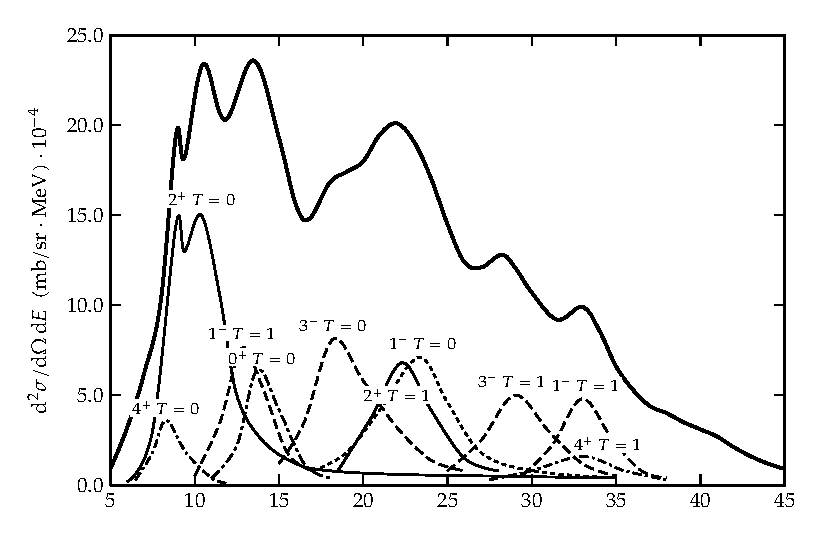
\includegraphics[width=0.8\textwidth]{pictures/8_6}
\par\end{centering}
\caption{\label{fig:8_6}基于微观 RPA 波函数计算得到的 $^{208}\mathrm{Pb}$ 在 $75^{\circ}$
散射角下 $90\,\text{MeV}$ 电子散射 $(e,e')$ 谱。图中的数字标明了相应截面贡献的角动量、宇称与同位旋。}
\end{figure}


\subsection{类似共振\label{subsec:8.3.4_=007C7B=004F3C=005171=00632F}}

重核（$N>Z$）的核反应（例如 $^{208}\mathrm{Pb}(p,n)^{208}\mathrm{Bi}$）表现出强烈的集体共振，由于我们即将阐述的原因，它们被称为类似态（analog
states）\footnote{相关文献可参见例如［AHK 72］。}。

为了解释这些态的结构，我们利用重核波函数在极佳近似下是同位旋算符 $\boldsymbol{T}^{2}$ 本征态的事实（参见第
2.6.3 节）。基态与低激发态具有量子数 $T=T_{z}=(N-Z)/2$。从能量为 $E_{n}$ 的态 $|I,T,T_{z}=T\rangle$
出发，我们可以通过施加同位旋降算符 $T_{-}$ 来定义其类似态：

\begin{equation}
T_{-}|I,T,T_{z}=T\rangle=\sqrt{2T}|I,T,T_{z}=T-1\rangle\label{eq:coll_analog_state_def}
\end{equation}

它属于“子核”（$N-1,Z+1$），且仍然是 $H$ 的本征态，能量为：

\begin{equation}
E_{A}=E_{n}+\Delta_{C}\label{eq:coll_analog_energy}
\end{equation}

为了理解这一点，我们将精确 Hamiltonian 量 $H$ 分解为与 $T_{-}$ 对易的强核力部分 $H_{\text{nucl}}$
以及 Coulomb 相互作用 $V_{c}$：

\begin{equation}
HT_{-}=(H_{\text{nucl}}+V_{c})T_{-}=T_{-}H+[V_{c},T_{-}]\label{eq:coll_ht_minus_commutator}
\end{equation}

对易子 $[V_{c},T_{-}]$ 具有如下形式：

\begin{equation}
[V_{c},T_{-}]=\sum^{A}_{i=1}v_{c}(i)t_{-}(i)\label{eq:coll_vc_tminus_commutator}
\end{equation}

式中平均 Coulomb 势为：

\begin{equation}
v_{c}(i)=\sum_{j\ne i}\frac{e^{2}}{|\boldsymbol{r}_{i}-\boldsymbol{r}_{j}|}\left(\frac{1}{2}-t_{z}(j)\right)\label{eq:coll_average_coulomb_potential}
\end{equation}

假定该单粒子势在核内部具有约 $\Delta_{C}$ 的常数值（参见图 2.7），我们便得到：母核（$N,Z$）的每个本征态
$|n\rangle$ 都在子核（$N-1,Z+1$）中对应着一个类似态 $T_{-}|n\rangle$：

\begin{equation}
HT_{-}|n\rangle=E_{n}T_{-}|n\rangle+[H,T_{-}]|n\rangle\approx(E_{n}+\Delta_{C})T_{-}|n\rangle\label{eq:coll_analog_schrodinger}
\end{equation}

这意味着在子核中存在一系列能级序列，其能级间距与母核本身的低激发能级完全相同，其同位旋为：

\begin{equation}
T=\frac{N-Z}{2}=\frac{(N-Z-2)}{2}+1\label{eq:coll_analog_isospin_plus_one}
\end{equation}

这比子核基态的同位旋大一个单位（\ref{fig:8_7}）。

\begin{figure}[H]
\begin{centering}
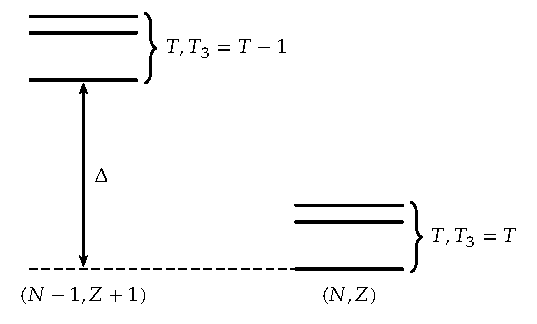
\includegraphics[width=0.5\textwidth]{pictures/8_7}
\par\end{centering}
\caption{\label{fig:8_7}类似态能谱示意图。}
\end{figure}

为了进一步了解类似共振的结构，我们暂时忽略在描述母核（$N,Z$）基态时所使用的剩余相互作用。后者由纯壳模型描述给出，如\ref{fig:8_8}
所示。

\begin{figure}[H]
\begin{centering}
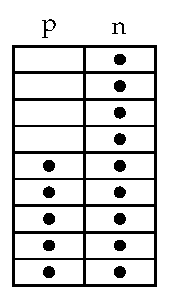
\includegraphics[width=0.25\textwidth]{pictures/8_8}
\par\end{centering}
\caption{\label{fig:8_8}纯壳模型行列式波函数的示意图。}
\end{figure}

我们假设占据相同量子数（除 $t_{z}$ 外）态的质子与中子构成一个惰性核心，并耦合为 $T=0$。在下文中我们将忽略该惰性核心，因此母核的基态由过剩中子描述。利用
$T_{-}=\sum_{i}t_{-}(i)$，我们得到子核的类似态：

\begin{equation}
|I,T,T_{z}=T-1\rangle=\frac{1}{\sqrt{2T}}T_{-}|I,T,T_{z}=T\rangle=\frac{1}{\sqrt{2T}}\sum_{k}a^{\dagger}_{pk}a_{nk}|0\rangle\label{eq:coll_analog_state_ph_expansion}
\end{equation}

式 (\ref{eq:coll_analog_state_ph_expansion}) 中的类似态是某些特定电荷交换粒子-空穴态的相干叠加，这些态是通过将母核基态中的中子逐个替换为处于相应单粒子态的质子而形成的。

当然，还存在与类似态 $|I,T,T_{z}=T-1\rangle$ 正交的其他态 $|A\rangle$，算符 $T_{+}$
将它们完全湮灭，因此它们必须具有同位旋 $T-1$，即子核基态的同位旋。在没有剩余相互作用时，它们与类似态简并并具有相同的自旋与宇称。在实验上，类似态表现为高能量处的极其尖锐的共振峰［AW
61］。它们的宽度之所以如此之小，是因为同位旋选择定则禁止其迅速衰变到构成连续谱背景的其他态中。

\subsection{对振动\label{subsec:8.3.5_=005BF9=00632F=0052A8}}

粒子-粒子相互作用不仅能将核子束缚在一起，还能在核反应中诱发出显著的集体效应。例如在 $^{208}\mathrm{Pb}(p,t)^{206}\mathrm{Pb}$
拾取反应或 $^{208}\mathrm{Pb}(t,p)^{210}\mathrm{Pb}$ 剥离反应截面中［Gl 65］，实验观测到
$^{206}\mathrm{Pb}$ 的 $0^{+}$ 基态的布居几率比 $^{206}\mathrm{Pb}$ 的其他
$0^{+}$ 态大整整一个数量级，这清楚地表明了 $C^{0^{+}}_{ij}$ 振幅的相干贡献以及该状态的强烈集体性。$^{210}\mathrm{Pb}$
的情形与此完全类似。处于 $0^{+}$ 态的两个粒子之间的这种强束缚实体源于相互作用的短程吸引部分，在第 6 章的开头已经对此进行了讨论。两个核子构成了如此稳定的配对实体，以至于它们可以像独立粒子一样（由于其整数自旋，其行为非常类似于玻色子）被成对地加到原子核（如
$^{208}\mathrm{Pb}$）中，或从中移除。因此，其能谱应当近似呈现出简谐振子的阶梯结构，而在铅同位素中实验观测确实如此（\ref{fig:8_9}）［BM
75］。这种谐振谱被称为“配对振动谱”（pairing vibrations）。

\begin{figure}[H]
\begin{centering}
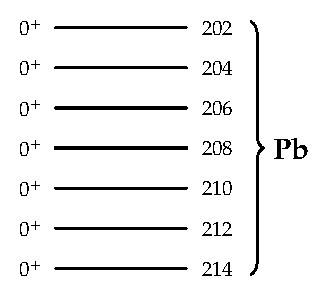
\includegraphics[width=0.4\textwidth]{pictures/8_9}
\par\end{centering}
\caption{\label{fig:8_9}偶数铅同位素基态能量的示意图。}
\end{figure}

我们同样可以在这些核中产生激发的 $0^{+}$ 对振动态。例如，从 $^{208}\mathrm{Pb}$ 中移除一个 $0^{+}$
配对声子使我们到达 $^{206}\mathrm{Pb}$；同时，加上一个从 $^{208}\mathrm{Pb}$ 到 $^{210}\mathrm{Pb}$
基态的声子，这显然在 $^{208}\mathrm{Pb}$ 中产生了一个能量约为 $2\hbar\Omega$ 的激发态。事实上，在
$^{210}\mathrm{Pb}(p,t)^{208}\mathrm{Pb}$ 和 $^{206}\mathrm{Pb}(t,p)^{208}\mathrm{Pb}$
反应中被强烈激发的这样一个态是众所周知的，它位于 $^{208}\mathrm{Pb}$ 的 $4.9\,\text{MeV}$
处。

粒子-粒子关联能够导致集体核运动模式（现通常称为对振动）这一事实，最早由 H. Schmidt［Sch 64a, b］和 Bohr［Bo
64］认识到，并在后来由 Bès 和 Broglia［BB 66］进行了极为详尽的研究（综述可参见［BHR 73］及相关文献）。

这是一个普遍的概念，它将配对关联置于与空间形变完全平等的地位上来描述。从球形闭壳核出发，我们可以激发与基态角动量不同的四极振动，也可以激发属于不同粒子数核的配对振动。由此类振动所诱发的基态关联（参见第
8.4.6 节），在第一种情况下给出了虚四极形变，在第二种情况下则给出了集体 2p-2h 态的虚激发。当我们远离闭壳层时，原子核变软，即关联增强。最终，我们经历相变：由
ph 关联诱发进入形变态；或者由 pp 关联诱发进入超流态。在超流核中，我们知道存在围绕稳定能隙参数的配对振动，正如变形核中存在围绕平衡形变的表面振动一样。

\section{含基态关联的粒子-空穴理论（RPA）\label{sec:8.4_=00542B=0057FA=006001=005173=008054=007684=007C92=005B50-=007A7A=007A74=007406=008BBA=00FF08RPA=00FF09}}

我们近似拟设 (\ref{eq:tda_ansatz_excited}) 的一个特征在于：我们能够在激发态中构建关联；然而在 TDA
方法中，基态却保持未关联。基态中对剩余相互作用 $V_{R}$ 的完全忽略无疑会影响计算结果。为了消除 TDA 方法的这一缺陷，人们可能会考虑在式
(\ref{eq:tda_expansion_ground}) 中同时保留 $(2p\text{-}2h)$ 分量。但这是不可行的，因为相应的矩阵维度将变得极其庞大。一条出路是对
TDA 方法进行推广：不再采用 HF 基态，而是采用一个对某一特定类别的关联进行了求和的基态。尽管对问题的讨论与 TDA 方法大致相同，但为了这种理论上的精细化，我们必须付出一定的代价：我们的新方程将不再直接遵循变分原理，因此原则上可能会出现虚数解。

我们将在与 TDA 方法紧密类比的基础上，采用一种不同的技术来推导这些新方程［随机相位近似（RPA）］\footnote{关于 RPA 历史文献与综述，参见例如［Boh 53, BP 53, Saw 57, Wo 58, Bro 64, Ro 70］。}，该技术将非常自然地引出通向
RPA 所需的推广。

\subsection{RPA 方程的推导\label{subsec:8.4.1_RPA=0065B9=007A0B=007684=0063A8=005BFC}}

为了更好地理解随机相位近似所做的工作，我们从 Hamilton 算符 $H$ 的一组精确本征态出发：

\begin{equation}
H|\nu\rangle=E_{\nu}|\nu\rangle,\quad H|0\rangle=E_{0}|0\rangle\label{eq:rpa_exact_eigenstates}
\end{equation}

总可以定义算符 $Q^{\dagger}_{\nu}$ 与 $Q_{\nu}$，使得：

\begin{equation}
|\nu\rangle=Q^{\dagger}_{\nu}|0\rangle\quad\text{且}\quad Q_{\nu}|0\rangle=0\label{eq:rpa_phonon_operators_def}
\end{equation}

例如，可选取 $Q^{\dagger}_{\nu}=|\nu\rangle\langle0|$。由 Schrödinger 方程
(\ref{eq:rpa_exact_eigenstates}) 可以得出运动方程：

\begin{equation}
[H,Q^{\dagger}_{\nu}]|0\rangle=(E_{\nu}-E_{0})Q^{\dagger}_{\nu}|0\rangle\label{eq:rpa_equation_of_motion}
\end{equation}

从左侧乘以形式为 $\langle0|\delta Q$ 的任意态，我们得到\footnote{这里 $\delta Q$ 由算符 $a^{\dagger}_{k}a_{l}$ 与系数 $C_{kl}$ 线性组合给出。}：

\begin{equation}
\langle0|[\delta Q,[H,Q^{\dagger}_{\nu}]]|0\rangle=\hbar\Omega_{\nu}\langle0|[\delta Q,Q^{\dagger}_{\nu}]|0\rangle\label{eq:rpa_double_commutator_eom}
\end{equation}

我们之所以能够使用对易子，是因为 $\langle0|Q^{\dagger}_{\nu}=\langle0|HQ^{\dagger}_{\nu}=0$。到目前为止的所有推导都是精确的；且由于
$\delta Q|0\rangle$ 的变分遍历整个 Hilbert 空间，式 (\ref{eq:rpa_double_commutator_eom})
等价于完整的 Schrödinger 方程 (\ref{eq:rpa_exact_eigenstates})。首先，我们通过用 HF
态 $|\text{HF}\rangle$ 近似精确基态 $|0\rangle$，并用集体 ph 算符近似算符 $Q^{\dagger}_{\nu}$：

\begin{equation}
Q^{\dagger}_{\nu}=\sum_{mi}C^{\nu}_{mi}a^{\dagger}_{m}a_{i}\label{eq:rpa_tda_limit_operator}
\end{equation}

来重新推导 TDA 方程 (\ref{eq:tda_secular_equation})。通过这种近似，我们将讨论局限于 1p-1h
激发空间，即设 $\delta Q|0\rangle=\sum_{mi}a^{\dagger}_{m}a_{i}|\text{HF}\rangle\delta C_{mi}$，并从式
(\ref{eq:rpa_double_commutator_eom}) 得到：

\begin{equation}
\sum_{nj}\langle\text{HF}|[a^{\dagger}_{i}a_{m},[H,a^{\dagger}_{n}a_{j}]]|\text{HF}\rangle C^{\nu}_{nj}=E^{\text{TDA}}_{\nu}C^{\nu}_{mi}\label{eq:rpa_rederive_tda}
\end{equation}

式中 $E^{\text{TDA}}_{\nu}$ 为 TDA 近似下的激发能量。这正是我们早先推导出的 TDA 方程 (\ref{eq:tda_secular_equation})。在这次推导中，我们并未借助于变分原理。然而，上述步骤的优势在于它可以直接推广。

完全没有任何理由阻止我们在式 (\ref{eq:rpa_tda_limit_operator}) 中采用更一般的振动产生算符，而正如我们即将看到的，这也意味着引入更一般的基态。若我们设想基态包含式
(\ref{eq:tda_expansion_ground}) 所示的 $2p\text{-}2h$ 关联，那么我们不仅能够产生一个
ph 对，而且能够销毁一个 ph 对。因此，式 (\ref{eq:rpa_tda_limit_operator}) 最自然的推广为：

\begin{equation}
Q^{\dagger}_{\nu}=\sum_{mi}\left(X^{\nu}_{mi}a^{\dagger}_{m}a_{i}-Y^{\nu}_{mi}a^{\dagger}_{i}a_{m}\right)\label{eq:rpa_creation_operator}
\end{equation}

其中负号是为了计算便利而选取的。RPA 基态 $|\text{RPA}\rangle$ 类比于式 (\ref{eq:rpa_phonon_operators_def})
定义为：

\begin{equation}
Q_{\nu}|\text{RPA}\rangle=0\label{eq:rpa_vacuum_condition}
\end{equation}

稍后我们将根据此条件导出基态的显式表达式。现在我们拥有两个矩阵 $X^{\nu}_{mi}$ 和 $Y^{\nu}_{mi}$，而非仅仅一个矩阵
$C^{\nu}_{mi}$。我们同样有两种变分 $\delta Q|0\rangle$，即 $a^{\dagger}_{m}a_{i}|0\rangle$
与 $a^{\dagger}_{i}a_{m}|0\rangle$。因此，从式 (\ref{eq:rpa_double_commutator_eom})
我们得到两组方程：

\begin{align}
\langle\text{RPA}|[a^{\dagger}_{i}a_{m},[H,Q^{\dagger}_{\nu}]]|\text{RPA}\rangle & =\hbar\Omega_{\nu}\langle\text{RPA}|[a^{\dagger}_{i}a_{m},Q^{\dagger}_{\nu}]|\text{RPA}\rangle,\nonumber \\
\langle\text{RPA}|[a^{\dagger}_{m}a_{i},[H,Q^{\dagger}_{\nu}]]|\text{RPA}\rangle & =\hbar\Omega_{\nu}\langle\text{RPA}|[a^{\dagger}_{m}a_{i},Q^{\dagger}_{\nu}]|\text{RPA}\rangle\label{eq:rpa_general_eom_pair}
\end{align}

式中 $\hbar\Omega_{\nu}$ 为态 $|\nu\rangle$ 的激发能。这些方程仅包含四个费米子算符的期望值，由于我们目前尚不知道基态
$|\text{RPA}\rangle$，计算它们仍然极其复杂。

我们满足于通常被称为“准玻色子近似”（quasi-boson approximation）的近似方法［BET 61, Br 64］。假定关联基态与
HF 基态相差不甚剧烈，我们可以在 HF 近似下计算所有期望值，例如：

\begin{equation}
\langle\text{HF}|[a^{\dagger}_{i}a_{m},a^{\dagger}_{n}a_{j}]|\text{HF}\rangle=\delta_{ij}\delta_{mn}\label{eq:rpa_quasiboson_commutation}
\end{equation}

“准玻色子”近似的名称源于这样一个事实：若 ph 产生与湮灭算符严格服从玻色子场算符的对易关系，则式 (\ref{eq:rpa_quasiboson_commutation})
将是一条精确等式。然而，式 (\ref{eq:rpa_quasiboson_commutation}) 破坏了 Pauli 原理，因为我们忽略了来自对易子的非对角项。这种近似的优良程度只能通过实际计算来检验（亦见第
9 章）。

在准玻色子近似下，振幅 $X^{\nu}_{mi}$ 与 $Y^{\nu}_{mi}$ 具有非常直接的物理意义：它们的模平方分别给出了在激发态
$|\nu\rangle$ 中找到态 $a^{\dagger}_{m}a_{i}|0\rangle$ 与 $a^{\dagger}_{i}a_{m}|0\rangle$
的几率，也就是式 (\ref{eq:coll_transition_density_matrix}) 中跃迁密度 $\rho^{(\nu)}$
的 ph 与 hp 矩阵元：

\begin{equation}
X^{\nu}_{mi}=\langle0|a^{\dagger}_{i}a_{m}|\nu\rangle=\rho^{(\nu)*}_{mi},\quad Y^{\nu}_{mi}=\langle0|a^{\dagger}_{m}a_{i}|\nu\rangle=\rho^{(\nu)*}_{im}\label{eq:rpa_xy_amplitudes_density}
\end{equation}

方程组 (\ref{eq:rpa_general_eom_pair}) 现可写为极其紧凑的矩阵形式：

\begin{equation}
\begin{pmatrix}A & B\\
B^{*} & A^{*}
\end{pmatrix}\begin{pmatrix}X^{\nu}\\
Y^{\nu}
\end{pmatrix}=\hbar\Omega_{\nu}\begin{pmatrix}1 & 0\\
0 & -1
\end{pmatrix}\begin{pmatrix}X^{\nu}\\
Y^{\nu}
\end{pmatrix}\label{eq:rpa_matrix_equation}
\end{equation}

其中 $(X^{\nu})_{mi}=X^{\nu}_{mi}$，$(Y^{\nu})_{mi}=Y^{\nu}_{mi}$，且：

\begin{align}
A_{minj} & =\langle\text{HF}|[a^{\dagger}_{i}a_{m},[H,a^{\dagger}_{n}a_{j}]]|\text{HF}\rangle=(\epsilon_{m}-\epsilon_{i})\delta_{mn}\delta_{ij}+\bar{v}_{mjin},\nonumber \\
B_{minj} & =-\langle\text{HF}|[a^{\dagger}_{i}a_{m},[H,a^{\dagger}_{j}a_{n}]]|\text{HF}\rangle=\bar{v}_{mnij}\label{eq:rpa_ab_matrices_def}
\end{align}

矩阵 $A$ 是 Hermitian 矩阵，矩阵 $B$ 是对称矩阵。

方程 (\ref{eq:rpa_matrix_equation}) 连同 (\ref{eq:rpa_ab_matrices_def})
被称为 RPA 方程。若令所有 $Y^{\nu}_{mi}=0$，我们即回到 TDA 方程。因此，$Y^{\nu}_{mi}$
是基态关联强弱的度量。

\begin{figure}[H]
\begin{centering}
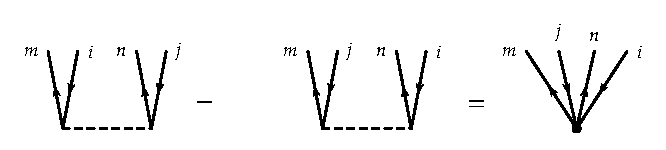
\includegraphics[width=0.75\textwidth]{pictures/8_10}
\par\end{centering}
\caption{\label{fig:8_10}方程 (\ref{eq:rpa_ab_matrices_def}) 中矩阵 $B$ 元素的图形表示。}
\end{figure}

正如观察式 (\ref{eq:rpa_ab_matrices_def}) 中的矩阵 $B$ 所见，除图 8.3 中的图形外，RPA
还包含了\ref{fig:8_10} 中所示的图形，它们具有虚 $2p\text{-}2h$ 激发的物理意义。

\subsection{RPA 的稳定性\label{subsec:8.4.2_RPA=007684=007A33=005B9A=006027}}

矩阵

\begin{equation}
\mathcal{S}=\begin{pmatrix}A & B\\
B^{*} & A^{*}
\end{pmatrix}\label{eq:rpa_stability_matrix_def}
\end{equation}

恰好是在式 (7.37) 中推导出的 HF 理论稳定性矩阵。它是一个 Hermitian 矩阵，其实数本征值表征了 HF 解的物理性质。若
$\mathcal{S}$ 是正定的，则它对应于能量曲面上的极小值点。在这种情况下，我们可以计算矩阵 $\mathcal{S}$
的平方根，并将本征值问题 (\ref{eq:rpa_matrix_equation}) 变换为更对称的形式：

\begin{equation}
\mathcal{S}^{1/2}\eta\mathcal{S}^{1/2}\left(\mathcal{S}^{1/2}\begin{pmatrix}X^{\nu}\\
Y^{\nu}
\end{pmatrix}\right)=\hbar\Omega_{\nu}\left(\mathcal{S}^{1/2}\begin{pmatrix}X^{\nu}\\
Y^{\nu}
\end{pmatrix}\right)\label{eq:rpa_s_half_hermitian}
\end{equation}

其中

\begin{equation}
\eta=\begin{pmatrix}1 & 0\\
0 & -1
\end{pmatrix}\label{eq:rpa_eta_metric_def}
\end{equation}

这是一个仅具有实数本征值的 Hermitian 本征值问题。换言之，若 HF 解对应于能量曲面上的极小值而非鞍点或极大值，则相应的
RPA 方程仅具有实数激发频率［Th 61a］。反之则未必成立。在下文中，我们将假定仅存在实数频率。

\subsection{归一化与完备性关系\label{subsec:8.4.3_=005F52=004E00=005316=004E0E=005B8C=005907=006027=005173=007CFB}}

由于 RPA 矩阵不是 Hermitian 矩阵，其本征矢在通常意义下并不正交。激发态 $|\nu\rangle=Q^{\dagger}_{\nu}|\text{RPA}\rangle$
相互正交的条件给出了正交性关系：

\begin{equation}
\langle\nu|\nu'\rangle=\langle\text{RPA}|[Q_{\nu},Q^{\dagger}_{\nu'}]|\text{RPA}\rangle=\sum_{mi}\left(X^{\nu*}_{mi}X^{\nu'}_{mi}-Y^{\nu*}_{mi}Y^{\nu'}_{mi}\right)=\delta_{\nu\nu'}\label{eq:rpa_orthonormality_condition}
\end{equation}

事实上，我们可以证明 $\nu\ne\nu'$ 的 RPA 方程的解严格满足这一关系。对于 $\nu=\nu'$，若其范数为正，这为我们提供了归一化矢量
$(X^{\nu},Y^{\nu})$ 的准则［Th 61a］。

引入如下矩阵十分便利：

\begin{equation}
\mathcal{X}=\begin{pmatrix}X & Y^{*}\\
Y & X^{*}
\end{pmatrix},\quad\Omega=\begin{pmatrix}\Omega_{\nu} & 0\\
0 & -\Omega_{\nu}
\end{pmatrix}\label{eq:rpa_big_x_matrix_def}
\end{equation}

此时，RPA 方程具有如下紧凑形式：

\begin{equation}
\mathcal{S}\mathcal{X}=\eta\mathcal{X}\hbar\Omega\label{eq:rpa_compact_matrix_form}
\end{equation}

简单的矩阵代数运算表明：

\begin{equation}
[\Omega,\mathcal{X}^{\dagger}\eta\mathcal{X}]=0\label{eq:rpa_commutator_omega_x}
\end{equation}

即 $\Omega$ 与 $\mathcal{X}^{\dagger}\eta\mathcal{X}$ 对易，因此 $\mathcal{X}^{\dagger}\eta\mathcal{X}$
与 $\Omega$ 同时对角化。由于矢量的归一化尚未确定，我们选取：

\begin{equation}
\mathcal{X}^{\dagger}\eta\mathcal{X}=\eta\label{eq:rpa_orthonormality_matrix_form}
\end{equation}

这正是正交归一化条件 (\ref{eq:rpa_orthonormality_condition})。完备性条件则通过将式 (\ref{eq:rpa_orthonormality_matrix_form})
两边乘以 $\eta$ 得到，表明 $\eta\mathcal{X}^{\dagger}$ 是 $\mathcal{X}$ 的逆矩阵：

\begin{equation}
\mathcal{X}\eta\mathcal{X}^{\dagger}=\eta\label{eq:rpa_completeness_matrix_form}
\end{equation}

显式写出即为：

\begin{align}
\sum_{\nu}\left(X^{\nu}_{mi}X^{\nu*}_{nj}-Y^{\nu*}_{mi}Y^{\nu}_{nj}\right) & =\delta_{mn}\delta_{ij},\nonumber \\
\sum_{\nu}\left(X^{\nu}_{mi}Y^{\nu*}_{nj}-Y^{\nu*}_{mi}X^{\nu}_{nj}\right) & =0\label{eq:rpa_closure_explicit}
\end{align}


\subsection{RPA 方程的数值求解\label{subsec:8.4.4_RPA=0065B9=007A0B=007684=006570=00503C=006C42=0089E3}}

在许多实际问题中，RPA 矩阵 $A$ 和 $B$ 均为实数。对于实频率 $\Omega_{\nu}$，求解问题可以简化为对角化一个维度仅为原维度一半的实对称矩阵。

我们定义矢量：

\begin{equation}
P^{\nu}=\frac{\mathrm{i}}{\sqrt{2}}(X^{\nu}+Y^{\nu}),\quad Q^{\nu}=\frac{1}{\sqrt{2}}(X^{\nu}-Y^{\nu})\label{eq:rpa_pq_vectors_def}
\end{equation}

由式 (\ref{eq:rpa_matrix_equation}) 容易推得：

\begin{align}
\mathrm{i}(A-B)Q^{\nu} & =\hbar\Omega_{\nu}P^{\nu},\nonumber \\
-\mathrm{i}(A+B)P^{\nu} & =\hbar\Omega_{\nu}Q^{\nu}\label{eq:rpa_pq_decoupled_system}
\end{align}

从而：

\begin{equation}
(A+B)(A-B)Q^{\nu}=\hbar^{2}\Omega^{2}_{\nu}Q^{\nu}\label{eq:rpa_squared_frequency_problem}
\end{equation}

伴随着稳定性矩阵 $\mathcal{S}$ 的正定性，矩阵 $(A\pm B)$ 同样正定。我们可以利用 Cholesky 分解将
$A-B$ 分解为下三角矩阵及其转置的乘积：

\begin{equation}
A-B=LL^{T}\label{eq:rpa_cholesky_decomposition}
\end{equation}

进而将求解转化为实对称本征值问题：

\begin{equation}
L^{T}(A+B)LR^{\nu}=\hbar^{2}\Omega^{2}_{\nu}R^{\nu}\label{eq:rpa_symmetric_eigenproblem}
\end{equation}

求出本征值 $\hbar\Omega_{\nu}$ 与正交归一本征矢 $R^{\nu}$ 后，便可恢复出正确归一化的 RPA 振幅
$X^{\nu}$ 和 $Y^{\nu}$。

\subsection{玻色子算符表象\label{subsec:8.4.5_=0073BB=008272=005B50=007B97=007B26=008868=008C61}}

在推导 RPA 方程 (\ref{eq:rpa_matrix_equation}) 时，我们采用了准玻色子近似 (\ref{eq:rpa_quasiboson_commutation})，即用玻色子算符
$B_{mi}$ 替代 ph 算符 $a^{\dagger}_{m}a_{i}$：

\begin{equation}
a^{\dagger}_{m}a_{i}\to B^{\dagger}_{mi},\quad a^{\dagger}_{i}a_{m}\to B_{mi}\label{eq:rpa_boson_mapping}
\end{equation}

它们满足严格的玻色子对易关系：

\begin{equation}
[B_{mi},B^{\dagger}_{nj}]=\delta_{mn}\delta_{ij},\quad[B_{mi},B_{nj}]=0\label{eq:rpa_boson_commutation_exact}
\end{equation}

在此表象下，保留至简谐阶次的玻色子 Hamiltonian 量为：

\begin{equation}
H_{B}=E_{\text{HF}}-\frac{1}{2}\operatorname{Tr}A+\frac{1}{2}\begin{pmatrix}B^{\dagger} & B\end{pmatrix}\begin{pmatrix}A & B\\
B^{*} & A^{*}
\end{pmatrix}\begin{pmatrix}B\\
B^{\dagger}
\end{pmatrix}\label{eq:rpa_boson_hamiltonian}
\end{equation}

通过引入玻色子 Bogoliubov 变换：

\begin{equation}
O^{\dagger}_{\nu}=\sum_{mi}\left(X^{\nu}_{mi}B^{\dagger}_{mi}-Y^{\nu}_{mi}B_{mi}\right)\label{eq:rpa_boson_bogoliubov}
\end{equation}

Hamiltonian 量 (\ref{eq:rpa_boson_hamiltonian}) 可被完全对角化为独立简谐振子的集合：

\begin{equation}
H_{B}=E_{\text{RPA}}+\sum_{\nu>0}\hbar\Omega_{\nu}O^{\dagger}_{\nu}O_{\nu}\label{eq:rpa_diagonal_boson_h}
\end{equation}

式中 RPA 基态能为：

\begin{equation}
E_{\text{RPA}}=E_{\text{HF}}-\sum_{\nu>0}\hbar\Omega_{\nu}\operatorname{Tr}(Y^{\nu\dagger}Y^{\nu})=E_{\text{HF}}-\frac{1}{2}\sum_{\nu>0}\left(E^{\text{TDA}}_{\nu}-\hbar\Omega_{\nu}\right)\label{eq:rpa_ground_energy_lowering}
\end{equation}

这表明由于基态关联的存在，RPA 基态能相对于 Hartree-Fock 基态能有所降低，其降低量恰好等于 RPA 与 TDA 各激发能之差总和的一半。

\subsection{RPA 基态的构造\label{subsec:8.4.6_RPA=0057FA=006001=007684=006784=009020}}

RPA 基态最初由式 (\ref{eq:rpa_vacuum_condition}) 定义为算符 $Q_{\nu}$ 的真空。在准玻色子近似下，它等价于玻色子算符
$O_{\nu}$ 的真空 $|\text{RPA}\rangle$：

\begin{equation}
O_{\nu}|\text{RPA}\rangle=0\label{eq:rpa_boson_vacuum_condition}
\end{equation}

类比于第 7 章利用准粒子 Thouless 定理构造真空的做法，我们可以通过 Thouless 定理［Th 60］从玻色子 $B_{mi}$
的真空 $|\text{HF}\rangle$ 显式构造出 RPA 基态：

\begin{equation}
|\text{RPA}\rangle=N_{0}\exp\left(\frac{1}{2}\sum_{minj}Z_{minj}B^{\dagger}_{mi}B^{\dagger}_{nj}\right)|\text{HF}\rangle\label{eq:rpa_thouless_ground_state}
\end{equation}

其中 $N_{0}$ 为归一化系数，且：

\begin{equation}
Z=Y^{*}X^{*-1}\label{eq:rpa_thouless_z_matrix}
\end{equation}

式 (\ref{eq:rpa_thouless_ground_state}) 表明，RPA 基态波函数包含了 $2p\text{-}2h,4p\text{-}4h,\dots$
等任意偶数粒子-空穴对的相干关联。

\subsection{不变性与赝解\label{subsec:8.4.7_=004E0D=0053D8=006027=004E0E=008D5D=0089E3}}

在下文中，我们假设精确的两体 Hamiltonian 量 $H$ 在由 Hermitian 单体算符 $P$ 所生成的连续对称操作下是不变的（例如全核质心平移的情况）；并进一步假定
HF 解破坏了该对称性。这特别意味着 HF 单粒子密度 $\rho^{(0)}$ 与 $P$ 不对易：

\begin{equation}
[\rho^{(0)},P]\ne0\label{eq:rpa_broken_symmetry_condition}
\end{equation}

由于 $\rho^{(0)}$ 在 HF 基下是对角的（对粒子能级为 0，对空穴能级为 1），这表明并非所有 ph 矩阵元 $P_{mi}$
都为零。由于精确 Hamiltonian 量与 $P$ 对易：

\begin{equation}
[H,P]=0\label{eq:rpa_exact_commutation_hp}
\end{equation}

因此 $P$ 是 RPA 方程的一个精确但属于赝模的解：

\begin{equation}
\begin{pmatrix}A & B\\
B^{*} & A^{*}
\end{pmatrix}\begin{pmatrix}P\\
-P^{*}
\end{pmatrix}=0\label{eq:rpa_spurious_zero_mode}
\end{equation}

式中 $P$ 为粒子-空穴空间中的矢量 $P_{mi}$。相应的态为：

\begin{equation}
P|\text{HF}\rangle=\sum_{mi}\left(P_{mi}a^{\dagger}_{m}a_{i}+P^{*}_{mi}a^{\dagger}_{i}a_{m}\right)|\text{HF}\rangle\label{eq:rpa_spurious_state_vector}
\end{equation}

我们认识到，RPA 方程 (\ref{eq:rpa_matrix_equation}) 仅在 HF 解确实破缺了该对称性时才具有此类解；否则矩阵元
$P_{mi}$ 恒等于零。

因此我们看到：只要我们在 RPA 中进行精确计算并采用自洽的单粒子能与波函数，对应于 HF 态中破缺对称性的赝激发（例如原子核作为整体的平移运动）就会完全自动解耦分离出来。它们与所有其他物理激发严格正交，且其激发能严格位于零能量处。这是
RPA 相比于 TDA 的重大优势所在，在 TDA 中赝解与真实物理态会发生严重的非物理混合。

为了求解与该零模共轭的正规坐标 $Q_{0}$，我们根据 Thouless 和 Valatin［TV 62］的方法建立非齐次方程组：

\begin{equation}
\begin{pmatrix}A & B\\
B^{*} & A^{*}
\end{pmatrix}\begin{pmatrix}Q_{0}\\
Q^{*}_{0}
\end{pmatrix}=\frac{\hbar}{\mathrm{i}M_{0}}\begin{pmatrix}P_{0}\\
-P^{*}_{0}
\end{pmatrix}\label{eq:rpa_thouless_valatin_eq}
\end{equation}

结合对易关系 $[Q_{0},P_{0}]=\mathrm{i}\hbar$，便可确定惯量参数 $M_{0}$。此时玻色子 Hamiltonian
量在零模与内禀振动之间完全解耦：

\begin{equation}
H_{B}=E_{\text{RPA}}+\frac{1}{2M_{0}}P^{2}_{0}+\sum_{\nu>0}\hbar\Omega_{\nu}O^{\dagger}_{\nu}O_{\nu}\label{eq:rpa_hamiltonian_with_zero_mode}
\end{equation}

对于平移运动，$M_{0}$ 恰为总核质量 $Am$；对于转动运动，$M_{0}$ 恰为著名的 Thouless-Valatin
转动惯量 $\mathcal{J}_{\text{TV}}$。

\section{线性响应理论\label{sec:8.5_=007EBF=006027=0054CD=005E94=007406=008BBA}}

在计算核系统的集体激发时，迄今为止我们均采用了定态 Schrödinger 方程 (\ref{eq:rpa_exact_eigenstates})，并尝试至少在某种近似下对角化
Hamiltonian 量。

现在我们将从一个截然不同的出发点展开研究。我们考查外加含时外场：

\begin{equation}
F(t)=Fe^{-\mathrm{i}\omega t}+F^{\dagger}e^{\mathrm{i}\omega t}\label{eq:linresp_external_field}
\end{equation}

对核系统的影响。我们假设 $F$ 是单体算符，且外场足够微弱，即它仅引起核密度的微小改变，使我们能够在满意的精度下在线性阶次内进行处理。

正如我们将看到的，核密度将随着该外场发生振荡；且每当外场频率 $\omega$ 接近系统的某一激发能量时，就会产生共振。通过这种途径：
\begin{enumerate}
\item 我们能够获取关于系统激发态的信息。特别地，我们找到了决定振幅 $\langle0|a^{\dagger}_{i}a_{m}|\nu\rangle$
的方程，它精确地对应于 RPA 方程。
\item 我们能够计算系统对外场的响应，即其密度、能量等物理量的动态改变。
\item 我们找到了一种为密度依赖相互作用推导 RPA 方程的普适方法。
\end{enumerate}

\subsection{线性响应方程的推导\label{subsec:8.5.1_=007EBF=006027=0054CD=005E94=0065B9=007A0B=007684=0063A8=005BFC}}

处于外加含时场中的核系统的波函数 $|\Phi(t)\rangle$ 不再是定态。它是一个波包，其单体密度：

\begin{equation}
\rho_{kk'}(t)=\langle\Phi(t)|a^{\dagger}_{k'}a_{k}|\Phi(t)\rangle\label{eq:linresp_density_matrix_def}
\end{equation}

此时显式地依赖于时间。我们希望在以下近似下显式计算该密度：
\begin{enumerate}
\item 我们假设在任何时刻 $\rho(t)$ 均对应于一个 Slater 行列式\footnote{即 $\rho^{2}=\rho$。在此意义下，以下对 RPA 的推导表明它正是独立粒子图像的含时推广（参见第 12 章）。}。此时
$\rho$ 服从如下运动方程：
\end{enumerate}
\begin{equation}
\mathrm{i}\hbar\dot{\rho}=[h[\rho]+f(t),\rho]\label{eq:linresp_tdhf_eom}
\end{equation}

这正是时间相关 Hartree-Fock（TDHF）方程。它将在第 12.2 节中详细推导。在此 $h[\rho]$ 是式 (5.33)
定义的单粒子 Hartree-Fock 场，而 $f(t)$ 是式 (\ref{eq:linresp_external_field})
的含时外场。
\begin{enumerate}
\item 我们假设外场 $f(t)$ 是微弱的，即它仅引起围绕定常密度 $\rho^{(0)}$ 的小振幅振荡，而 $\rho^{(0)}$
本身是定态 Hartree-Fock 方程 $[h[\rho^{(0)}],\rho^{(0)}]=0$ 的自洽解。因此，密度具有如下形式：
\end{enumerate}
\begin{equation}
\rho(t)=\rho^{(0)}+\delta\rho(t)\label{eq:linresp_density_split}
\end{equation}

其中

\begin{equation}
\delta\rho(t)=\rho^{(1)}e^{-\mathrm{i}\omega t}+\rho^{(1)\dagger}e^{\mathrm{i}\omega t}\label{eq:linresp_deltarho_fourier}
\end{equation}

线性地依赖于外场 $f$。在下文中，我们在使 $\rho^{(0)}$ 与 $h[\rho^{(0)}]$ 同时对角化的基矢——即自洽
HF 单粒子基——下开展讨论：

\begin{align}
\rho^{(0)}_{kk'} & =\delta_{kk'}\times\begin{cases}
1, & \text{对空穴能级},\\
0, & \text{对粒子能级},
\end{cases}\label{eq:linresp_rho0_diagonal}\\
(h_{0})_{kk'} & =(h[\rho^{(0)}])_{kk'}=\delta_{kk'}\epsilon_{k}\label{eq:linresp_h0_diagonal}
\end{align}

将式 (\ref{eq:linresp_density_split}) 代入 TDHF 方程 (\ref{eq:linresp_tdhf_eom})
并展开至外场 $f$ 的一阶线性项，得到：

\begin{equation}
\mathrm{i}\hbar\delta\dot{\rho}=[h_{0},\delta\rho]+\left[\frac{\delta h}{\delta\rho}\cdot\delta\rho,\rho^{(0)}\right]+[f(t),\rho^{(0)}]\label{eq:linresp_linearized_eom}
\end{equation}

式中 $\frac{\delta h}{\delta\rho}\cdot\delta\rho$ 是对下式的简写：

\begin{equation}
\left(\frac{\delta h}{\delta\rho}\cdot\delta\rho\right)_{kk'}=\sum_{ll'}\frac{\delta h_{kk'}}{\delta\rho_{ll'}}\delta\rho_{ll'}\label{eq:linresp_deltah_chain}
\end{equation}

利用 Slater 行列式条件 $\rho^{2}=\rho$ 导出的关系 $\rho^{(0)}\delta\rho+\delta\rho\rho^{(0)}=\delta\rho$，可以证明
$\delta\rho$ 仅具有粒子-空穴（ph）与空穴-粒子（hp）矩阵元。将式 (\ref{eq:linresp_linearized_eom})
投影到 ph 与 hp 基上，便得到线性响应方程组：

\begin{equation}
\begin{pmatrix}A-\hbar\omega & B\\
B^{*} & A^{*}+\hbar\omega
\end{pmatrix}\begin{pmatrix}\rho^{(1)}_{mi}\\
\rho^{(1)}_{im}
\end{pmatrix}=-\begin{pmatrix}f_{mi}\\
f_{im}
\end{pmatrix}\label{eq:linresp_matrix_system}
\end{equation}

式中矩阵 $A$ 与 $B$ 定义为：

\begin{align}
A_{minj} & =(\epsilon_{m}-\epsilon_{i})\delta_{mn}\delta_{ij}+\frac{\delta h_{mi}}{\delta\rho_{nj}},\nonumber \\
B_{minj} & =\frac{\delta h_{mi}}{\delta\rho_{jn}}\label{eq:linresp_ab_functional_derivative}
\end{align}

对于密度无关的两体相互作用，式 (\ref{eq:linresp_ab_functional_derivative}) 精确地退化为我们在第
8.4.1 节式 (\ref{eq:rpa_ab_matrices_def}) 中定义的矩阵元。然而，式 (\ref{eq:linresp_ab_functional_derivative})
的深远意义在于它同样适用于任何密度依赖的有效力（例如 Skyrme 力或 Gogny 力），此时剩余相互作用由能量泛函对密度的二阶泛函微商给出。

将式 (\ref{eq:linresp_matrix_system}) 形式求逆，可将系统的动态响应写为响应函数（极化传播子）$R(\omega)$
的作用：

\begin{equation}
\rho^{(1)}_{pq}=\sum_{p'q'}R_{pq,p'q'}(\omega)f_{p'q'}\label{eq:linresp_response_function_action}
\end{equation}

在零外场（$f=0$）下，式 (\ref{eq:linresp_matrix_system}) 的齐次方程恰好对应于响应函数 $R(\omega)$
的极点条件 $\omega=\Omega_{\nu}$：

\begin{equation}
\begin{pmatrix}A & B\\
B^{*} & A^{*}
\end{pmatrix}\begin{pmatrix}X^{\nu}\\
Y^{\nu}
\end{pmatrix}=\hbar\Omega_{\nu}\begin{pmatrix}1 & 0\\
0 & -1
\end{pmatrix}\begin{pmatrix}X^{\nu}\\
Y^{\nu}
\end{pmatrix}\label{eq:linresp_rpa_eigen_recovered}
\end{equation}

这正是 RPA 方程！它证明了：RPA 近似本质上就是含时平均场理论的小振幅极限。

借助 RPA 的完整本征解集，响应函数 $R(\omega)$ 可显式写为其谱表象（Lehmann 表象）：

\begin{equation}
R_{pq,p'q'}(\omega)=\sum_{\nu>0}\left[\frac{\rho^{(\nu)}_{pq}\rho^{(\nu)*}_{p'q'}}{\hbar(\omega-\Omega_{\nu}+\mathrm{i}\eta)}-\frac{\rho^{(\nu)*}_{qp}\rho^{(\nu)}_{q'p'}}{\hbar(\omega+\Omega_{\nu}+\mathrm{i}\eta)}\right]\label{eq:linresp_spectral_representation}
\end{equation}

它服从著名的 Bethe-Salpeter 方程：

\begin{equation}
R(\omega)=R^{0}(\omega)+R^{0}(\omega)\bar{v}R(\omega)\label{eq:linresp_bethe_salpeter}
\end{equation}

式中 $R^{0}(\omega)$ 为无剩余相互作用时的自由响应函数（独立粒子响应函数）。

\subsection{激发几率的计算与示意模型\label{subsec:8.5.2_=006FC0=0053D1=0051E0=007387=007684=008BA1=007B97=004E0E=00793A=00610F=006A21=00578B}}

在示意模型中，剩余相互作用采用可分离形式 $\bar{v}_{mjin}=\chi D_{mi}D^{*}_{nj}$［式 (\ref{eq:tda_separable_force})］，此时由式
(\ref{eq:linresp_bethe_salpeter}) 容易导出如下色散关系：

\begin{equation}
\frac{1}{\chi}=R^{0}_{D}(\Omega_{\nu})=\sum_{mi}|D_{mi}|^{2}\frac{2\epsilon_{mi}}{\hbar^{2}\Omega^{2}_{\nu}-\epsilon^{2}_{mi}}\label{eq:linresp_schematic_dispersion}
\end{equation}

\begin{figure}[H]
\begin{centering}
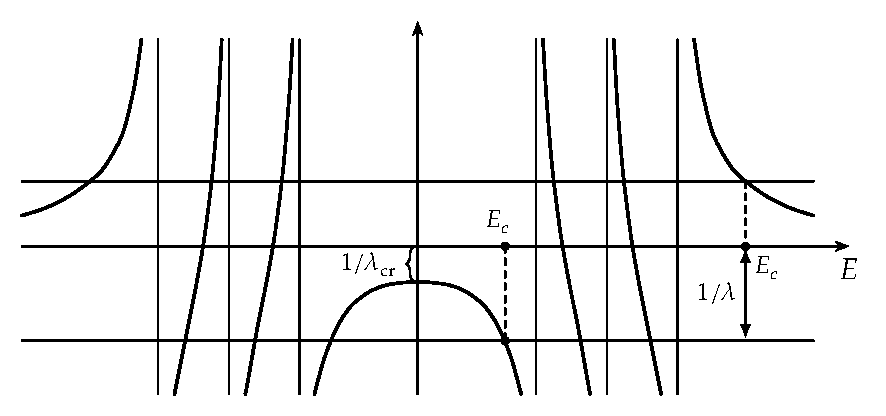
\includegraphics[width=0.75\textwidth]{pictures/8_11}
\par\end{centering}
\caption{\label{fig:8_11}色散关系 (\ref{eq:linresp_schematic_dispersion}) 的图解。}
\end{figure}

方程 (\ref{eq:linresp_schematic_dispersion}) 可以通过与 TDA 情形相同的方式在图形上求解。对比\ref{fig:8_11}
与图 8.4，我们可以注意到源于 RPA 基态关联的两个质的差异：
\begin{enumerate}
\item 当剩余相互作用强于某一临界值（即 $\chi<\chi_{\text{crit}}$）时，低激发集体态的能量变为纯虚数，标志着球形基态对形变破缺发生失稳。
\item 对于可比的相互作用强度 $\chi$，$T=0$ 的 RPA 集体态比对应的 TDA 态被向下拉得更低。
\end{enumerate}
在简并情形（所有 $\epsilon_{mi}=\epsilon$）下，集体态能量显式给出为：

\begin{equation}
E^{2}_{\text{coll}}=\hbar^{2}\Omega^{2}_{\text{coll}}=\epsilon^{2}+2\epsilon\chi\sum_{mi}|D_{mi}|^{2}\label{eq:linresp_degenerate_energy_squared}
\end{equation}

临界耦合强度为：

\begin{equation}
\chi_{\text{crit}}=-\frac{\epsilon}{2\sum_{mi}|D_{mi}|^{2}}\label{eq:linresp_critical_coupling}
\end{equation}

这正是球形 HF 解不再对应能量极小值的点，系统在此处发生从球形相到形变相的相变。在 TDA 中，相应的相变直到 $2\chi_{\text{crit}}$
处才发生。

计算响应函数 $R_{D}(\omega)$ 在极点 $\omega=\Omega_{\nu}$ 处的留数，给出到集体态的跃迁几率：

\begin{equation}
|\langle\nu|D|0\rangle|^{2}=\frac{\epsilon}{E_{\text{coll}}}\sum_{mi}|D_{mi}|^{2}\label{eq:linresp_enhanced_transition_prob}
\end{equation}

可以看到，对于低激发集体态，跃迁几率相比于 TDA 结果 (\ref{eq:tda_collective_transition_prob})
进一步放大了 $\epsilon/E_{\text{coll}}$ 倍。对于低激发的集体八极和四极态，该增强因子可高达 2 左右。

\subsection{静态极化率与转动惯量\label{subsec:8.5.3_=009759=006001=006781=005316=007387=004E0E=008F6C=0052A8=0060EF=0091CF}}

我们可以应用线性响应理论计算核系统在静态外场 $-\lambda F$ 下的能量改变与形变。这相当于在线性响应理论中求解受约束 Hartree-Fock（CHF）方程：

\begin{equation}
\delta\langle\Phi|H-\lambda F|\Phi\rangle=0\label{eq:linresp_chf_equation}
\end{equation}

由式 (\ref{eq:linresp_matrix_system})，零频极限下的密度改变量为：

\begin{equation}
\rho^{(1)}=\lambda\mathcal{S}^{-1}f\label{eq:linresp_static_density_response}
\end{equation}

静态极化率 $\alpha$ 定义为算符 $F$ 的期望值变化：

\begin{equation}
\delta\langle F\rangle=\operatorname{Tr}(F\delta\rho)=\alpha\lambda\label{eq:linresp_polarizability_def}
\end{equation}

体系能量的相应改变为：

\begin{equation}
\delta E=-\frac{1}{2}\alpha\lambda^{2}\label{eq:linresp_energy_second_order}
\end{equation}

由能量曲面在极小值点 $\lambda=0$ 处的曲率，我们得到静态极化率：

\begin{equation}
\alpha=\frac{\mathrm{d}^{2}E}{\mathrm{d}\lambda^{2}}=f^{\dagger}\mathcal{S}^{-1}f=2\sum_{\nu>0}\frac{|\langle\nu|F|0\rangle|^{2}}{\hbar\Omega_{\nu}}\label{eq:linresp_polarizability_sum_rule}
\end{equation}

这表明静态极化率与反能量加权求和规则 $S_{-1}$ 紧密联系在一起。

将上述形式体系应用于自洽推转模型（cranking model，参见第 7.7 节），外加约束场为推转算符 $\omega J_{x}$。线性响应方程即给出著名的
Thouless-Valatin 方程：

\begin{equation}
\mathcal{S}\delta\rho^{(1)}=\omega J_{x}\label{eq:linresp_tv_cranking_eq}
\end{equation}

进而给出完整的 Thouless-Valatin 自洽微观转动惯量：

\begin{equation}
\mathcal{J}_{\text{TV}}=\frac{\mathrm{d}^{2}E}{\mathrm{d}\omega^{2}}=2\sum_{\nu>0}\frac{|\langle\nu|J_{x}|0\rangle|^{2}}{\hbar\Omega_{\nu}}\label{eq:linresp_thouless_valatin_inertia}
\end{equation}


\subsection{连续谱中的 RPA 方程\label{subsec:8.5.4_=008FDE=007EED=008C31=004E2D=007684RPA=0065B9=007A0B}}

在实际的原子核巨共振激发中，单粒子能量通常高于粒子分离阈，核子可以发射到连续谱中。因此，真实问题并非离散的束缚态本征值问题，而是具有连续能量本征值的散射与共振问题。物理上关心的核心量是跃迁强度函数：

\begin{equation}
S_{F}(\omega)=\sum_{\nu>0}|\langle\nu|F|0\rangle|^{2}\delta(\hbar\omega-\hbar\Omega_{\nu})=-\frac{1}{\pi}\operatorname{Im}R_{F}(\omega)\label{eq:linresp_strength_function_im_r}
\end{equation}

巨共振在连续谱中的物理宽度源于两个截然不同的物理机制：
\begin{enumerate}
\item 衰变宽度（出射宽度，decay width $\Gamma^{\uparrow}$）：波函数中的单粒子分量处于 HF 势的连续散射态上，核子可以直接隧穿逸出衰变为自由粒子和
$A-1$ 核的空穴态。
\item 展宽宽度（扩散宽度，spreading width $\Gamma^{\downarrow}$）：ph 激发组态与更为复杂的 $2p\text{-}2h$
及更高级复合核组态相耦合，使跃迁强度弥散在密集的背景态之中。
\end{enumerate}
对于具有零力程相互作用（例如 Skyrme 力）的核系统，Bertsch、Tsai、Shlomo、Liu 等人［Be 73, SB
75, BT 75, LG 76b］发展了在坐标空间中求解 Bethe-Salpeter 方程的强大技术。引入单粒子 Green 函数：

\begin{equation}
G(\boldsymbol{r},\boldsymbol{r}',\omega)=\langle\boldsymbol{r}|\frac{1}{\hbar\omega-h_{0}+\mathrm{i}\eta}|\boldsymbol{r}'\rangle=-\frac{2m}{\hbar^{2}}\sum_{ljm}\frac{v_{lj}(r_{<})w_{lj}(r_{>})}{W(v,w)}Y_{ljm}(\hat{\boldsymbol{r}})Y^{*}_{ljm}(\hat{\boldsymbol{r}}')\label{eq:linresp_single_particle_green}
\end{equation}

其中 $v(r)$ 与 $w(r)$ 分别为在原点正则与在无穷远满足出射波边界条件的两个线性无关单粒子解，$W(v,w)$ 为其
Wronskian 决定式。无相互作用响应函数 $R^{0}(\boldsymbol{r},\boldsymbol{r}',\omega)$
即可闭合表达为束缚空穴波函数与该 Green 函数的折积：

\begin{equation}
R^{0}(\boldsymbol{r},\boldsymbol{r}',\omega)=\sum_{i}\left[\phi^{*}_{i}(\boldsymbol{r})\phi_{i}(\boldsymbol{r}')G(\boldsymbol{r},\boldsymbol{r}',\epsilon_{i}+\hbar\omega)+\phi_{i}(\boldsymbol{r})\phi^{*}_{i}(\boldsymbol{r}')G(\boldsymbol{r}',\boldsymbol{r},\epsilon_{i}-\hbar\omega)\right]\label{eq:linresp_r0_coordinate_space}
\end{equation}

在此基础上，全响应函数满足坐标空间一维积分方程：

\begin{equation}
R(\boldsymbol{r},\boldsymbol{r}',\omega)=R^{0}(\boldsymbol{r},\boldsymbol{r}',\omega)+V_{0}\int\mathrm{d}^{3}r''R^{0}(\boldsymbol{r},\boldsymbol{r}'',\omega)R(\boldsymbol{r}'',\boldsymbol{r}',\omega)\label{eq:linresp_coordinate_bethe_salpeter}
\end{equation}

利用球谐函数展开将角向坐标积出后，式 (\ref{eq:linresp_coordinate_bethe_salpeter}) 化为径向坐标网格点上的非齐次代数线性方程组，其数值求解极为高效，且严格精确地包含了连续谱边界条件。

\section{应用及与实验的比较\label{sec:8.6_=005E94=007528=0053CA=004E0E=005B9E=009A8C=007684=006BD4=008F83}}

\subsection{唯象基下的粒子-空穴计算\label{subsec:8.6.1_=00552F=008C61=0057FA=004E0B=007684=007C92=005B50-=007A7A=007A74=008BA1=007B97}}

早在 1957 年，Elliott 和 Flowers［EF 57］就针对双幻核 $^{16}\mathrm{O}$ 的负宇称态进行了开创性的
TDA 计算。他们采用了谐振子基，组态空间包含用于 $1^{-}$ 通道的 5 个 ph 态以及用于 $3^{-}$ 通道的 3
个 ph 态。采用带有 Rosenfeld 交换混合的 Yukawa 相互作用［EF 57, 表 4.3］，他们发现在约 $7\,\text{MeV}$
处存在一个高度集体的 $3^{-},\,T=0$ 态，以及在 $22.6\,\text{MeV}$ 和 $25.2\,\text{MeV}$
处的两个集体 $1^{-},\,T=1$ 态。在该组态空间中，八极态耗尽了 68\% 的 $S_{0}$ 求和规则，两个偶极态耗尽了
97\% 的求和规则。这在定性上与示意模型（第 8.2.2 节）的结果完全一致。跃迁强度主要集中在从无微扰单粒子能量（约 $11.5\,\text{MeV}$）显著移开的一个能级上。

Gillet 等人［Gi 64, GV 64, GS 64, GGS 66］通过在闭壳核 $^{12}\mathrm{C}$、$^{16}\mathrm{O}$、$^{40}\mathrm{Ca}$
和 $^{208}\mathrm{Pb}$ 中对比 TDA 与 RPA 计算，系统研究了基态关联的影响。他们发现，对于 $T=1$
能级，RPA 的结果与 TDA 相比变化不大；然而低激发的 $T=0$ 态在 RPA 中得到了好得多的重现。特别是 RPA 的激发几率显著大于
TDA 的值。

Ring 和 Speth［RS 74a］应用了由 Migdal［Mi 67］发展的有限费米系统理论。该理论从截然不同的视角出发，用短程且依赖于密度的重整化有效相互作用［式
(4.113)］来描述准粒子与准空穴之间的相互作用，并以计算集体态的 RPA 方程告终。在铅同位素区域［RS 73, RS 74a］，他们采用
Woods-Saxon 基展开、包含费米面上下各两个主壳的大组态空间，计算了 $^{208}\mathrm{Pb}$ 的低激发态能谱与跃迁几率，列于表
8.1 中。

\begin{table}[H]
\caption{\label{tab:8_1}基于 Migdal 力在 RPA 理论下计算得到的 $^{208}\mathrm{Pb}$ 低激发集体态的能量与激发几率［RS
74a］。}

\centering{}%
\begin{tabular}{cccccc}
\hline 
$I^{\pi}$ & \multicolumn{2}{c}{$E(I)\,[\text{MeV}]$} & \multicolumn{2}{c}{$B(E/M)I$} & 单位\tabularnewline
\hline 
 & 理论 & 实验 & 理论 & 实验 & \tabularnewline
\hline 
$3^{-}$ & 2.63 & 2.61 & 546 & $(540\pm30)\times10^{3}$ & $e^{2}\,\text{fm}^{6}$\tabularnewline
$5^{-}$ & 3.39 & 3.19 & 285 & $(462\pm55)\times10^{6}$ & $e^{2}\,\text{fm}^{10}$\tabularnewline
$5^{-}$ & 3.82 & 3.71 & 301 & $330\times10^{6}$ & $e^{2}\,\text{fm}^{10}$\tabularnewline
$2^{+}$ & 4.49 & 4.07 & 3070 & 2965 & $e^{2}\,\text{fm}^{4}$\tabularnewline
$4^{+}$ & 4.69 & 4.32 & 757 & $1287\times10^{4}$ & $e^{2}\,\text{fm}^{8}$\tabularnewline
$6^{+}$ & 4.77 & 4.42 & 210 & $230\times10^{8}$ & $e^{2}\,\text{fm}^{12}$\tabularnewline
$1^{+}$ & 7.50 & 7.56 & 568 & 5.9 & $\mu^{2}_{N}$\tabularnewline
$1^{+}$ & 8.30 & 7.99 & 11.00 & 10.0 & $\mu^{2}_{N}$\tabularnewline
$2^{-}$ & 7.51 & — & $11.00\times10^{3}$ & — & $\mu^{2}_{N}\,\text{fm}^{2}$\tabularnewline
\hline 
\end{tabular}
\end{table}

\begin{figure}[H]
\begin{centering}
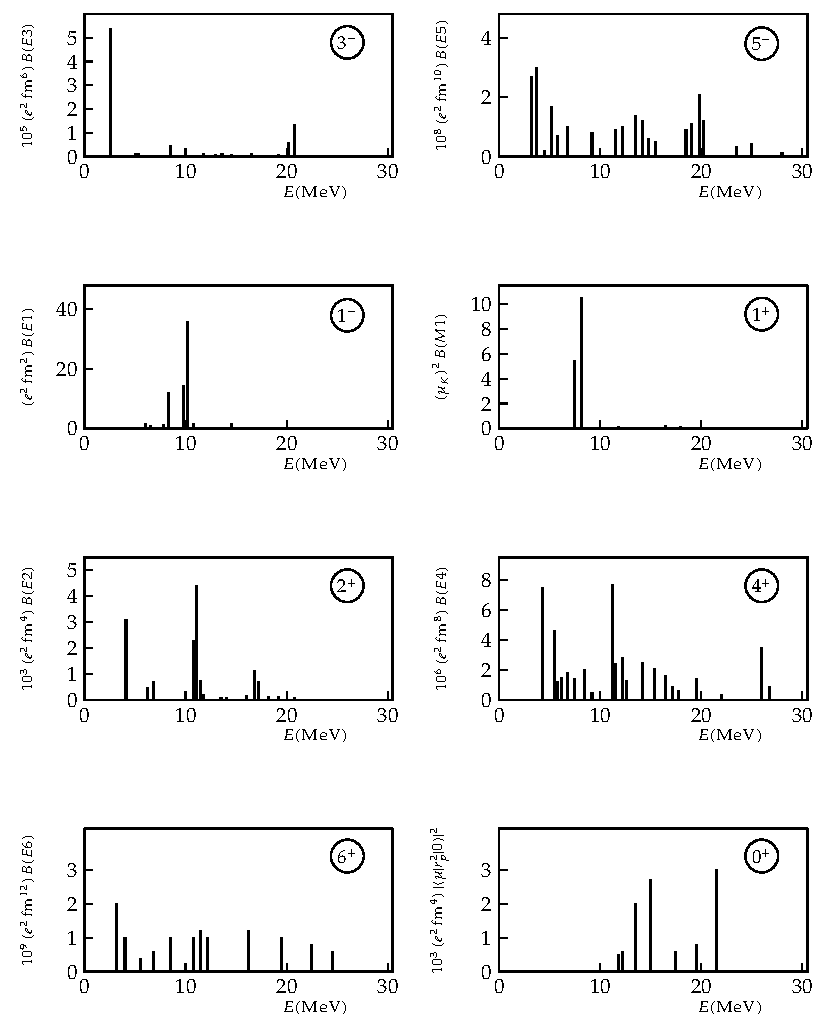
\includegraphics[width=0.8\textwidth]{pictures/8_12}
\par\end{centering}
\caption{\label{fig:8_12}$^{208}\mathrm{Pb}$ 中多极跃迁强度的分布（引自 \cite{RS74a}）。}
\end{figure}

\ref{fig:8_12} 展示了强度的分布情况。特别是，它不仅展示了低激发的 $3^{-},2^{+},4^{+},6^{+}$
集体态，还展示了巨共振，如 $1^{-}$（其能量略微偏低）、$2^{+}$（分裂为 $T=0$ 部分和 $T=1$ 部分）、位于约
$14\,\text{MeV}$ 处的呼吸模（$0^{+}$）以及更高极次的共振。

\subsection{自洽基下的粒子-空穴计算\label{subsec:8.6.2_=0081EA=006D3D=0057FA=004E0B=007684=007C92=005B50-=007A7A=007A74=008BA1=007B97}}

正如我们在第 5 章所见，采用唯象密度依赖有效力（如 Skyrme 力）的 Hartree-Fock 理论能够极好地重现基态性质。在自洽基下，RPA
的剩余相互作用由总能量泛函对密度的二阶泛函微商给出。近年来，Bertsch 等人［BT 75, LB 76, BGG 76, KKS
77］将该自洽理念应用于连续谱 RPA 计算中。

\begin{figure}[H]
\begin{centering}
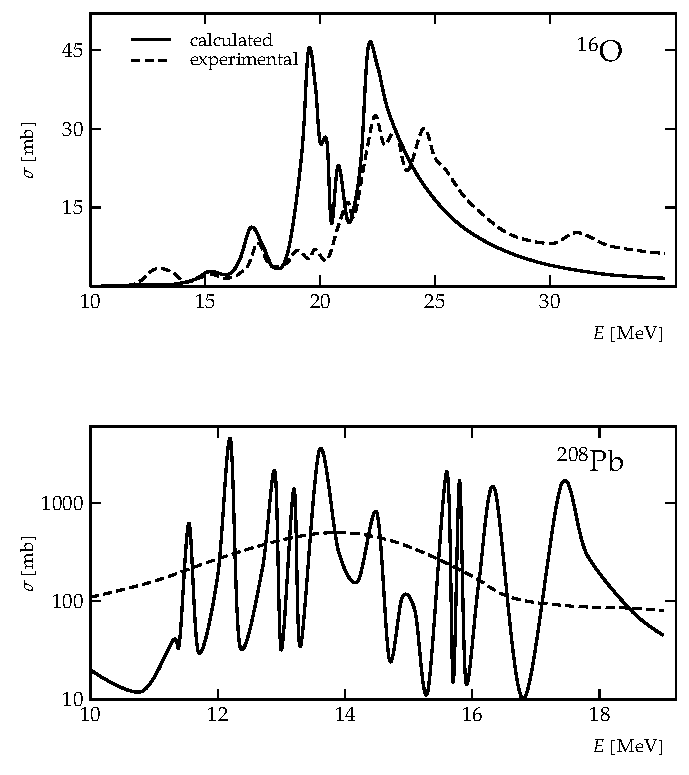
\includegraphics[width=0.8\textwidth]{pictures/8_13}
\par\end{centering}
\caption{\label{fig:8_13}基于连续谱 RPA 计算得到的 $^{16}\mathrm{O}$ 与 $^{208}\mathrm{Pb}$
巨偶极共振光吸收截面。虚线对应于实验值（引自 \cite{LG76b}）。}
\end{figure}

在\ref{fig:8_13} 中，我们看到连续谱 RPA 能够直接计算出巨偶极共振的线宽与出射谱。然而，理论曲线在 $^{208}\mathrm{Pb}$
中呈现出许多尖锐的共振峰，这是由于目前的 RPA 计算仅包含了出射宽度 $\Gamma^{\uparrow}$，未包含源于与 $2p\text{-}2h$
等复杂组态耦合引起的扩散宽度 $\Gamma^{\downarrow}$。

\section{求和规则\label{sec:8.7_=006C42=00548C=0089C4=005219}}

\subsection{强度函数的能量加权矩\label{subsec:8.7.1_=005F3A=005EA6=0051FD=006570=007684=0080FD=0091CF=0052A0=006743=0077E9}}

对于厄米单体算符 $F=\sum_{p}f(\boldsymbol{r}_{p})$，求和规则定义为强度分布的 $k$ 阶矩：

\begin{equation}
S_{k}(F)=\sum_{\nu>0}(E_{\nu}-E_{0})^{k}|\langle\nu|F|0\rangle|^{2}\label{eq:sumrule_moment_def}
\end{equation}

利用完备性关系，可写为：

\begin{equation}
S_{k}=\langle0|F(H-E_{0})^{k}F|0\rangle\label{eq:sumrule_operator_moment}
\end{equation}

根据 Lane 等人［MBF 76, BML 76, BLM 79］的研究，可以定义表征强度分布的特征能量：

\begin{equation}
\bar{E}_{k}=\sqrt{\frac{S_{k}}{S_{k-2}}}\label{eq:sumrule_average_energy_def}
\end{equation}

由 Schwarz 不等式 $S_{k+2}S_{k}\ge S^{2}_{k+1}$，可以导出 $\bar{E}_{3}\ge\bar{E}_{1}$，并且围绕平均能量的均方涨落满足：

\begin{equation}
\sigma^{2}=\bar{E}^{2}-\bar{E}^{2}_{1}\le\frac{1}{4}\left(\bar{E}^{2}_{3}-\bar{E}^{2}_{1}\right)\label{eq:sumrule_energy_dispersion_bound}
\end{equation}


\subsection{$S_{1}$ 求和规则与 RPA 方法\label{subsec:8.7.2_S1=006C42=00548C=0089C4=005219=004E0ERPA=0065B9=006CD5}}

最重要的求和规则是能量加权求和规则（EWSR）$S_{1}$。它可以精确表达为双对易子的基态期望值：

\begin{equation}
S_{1}(F)=\frac{1}{2}\langle0|[F,[H,F]]|0\rangle\label{eq:sumrule_double_commutator_exact}
\end{equation}

Thouless［Th 61a］证明了一条极为优美的定理：若左端项采用 RPA 激发能量与跃迁振幅计算，而右端项在自洽 Hartree-Fock
基态下求值，则等式 (\ref{eq:sumrule_double_commutator_exact}) 严格成立：

\begin{equation}
\sum_{\nu>0}\hbar\Omega_{\nu}|\langle\nu|F|0\rangle_{\text{RPA}}|^{2}=\frac{1}{2}\langle\text{HF}|[F,[H,F]]|\text{HF}\rangle\label{eq:sumrule_thouless_theorem_rpa}
\end{equation}


\subsection{求和规则 $S_{1},S_{-1},S_{3}$ 的求值\label{subsec:8.7.3_=006C42=00548C=0089C4=005219=007684=006C42=00503C}}

对于坐标空间中的局域单体算符 $F(\boldsymbol{r})$，它与速度无关的两体势严格对易，动能项对双对易子的贡献为：

\begin{equation}
[F,[H,F]]=\frac{\hbar^{2}}{m}\sum^{A}_{i=1}|\boldsymbol{\nabla}F(\boldsymbol{r}_{i})|^{2}\label{eq:sumrule_kinetic_double_commutator}
\end{equation}

因此 $S_{1}$ 求和规则由基态核密度直接给出：

\begin{equation}
S_{1}(F)=\frac{\hbar^{2}}{2m}\int|\boldsymbol{\nabla}F(\boldsymbol{r})|^{2}\rho_{0}(\boldsymbol{r})\,\mathrm{d}^{3}r\label{eq:sumrule_s1_density_integral}
\end{equation}

对于多极算符 $F_{LM}=r^{L}Y_{LM}$（$L\ge1$），式 (\ref{eq:sumrule_s1_density_integral})
给出：

\begin{equation}
S_{1}(r^{L}Y_{L0})=\frac{\hbar^{2}}{8\pi m}L(2L+1)A\langle r^{2L-2}\rangle\label{eq:sumrule_multipole_ewsr}
\end{equation}

对于单极算符 $F_{0}=\sum_{i}r^{2}_{i}$，我们得到：

\begin{equation}
S_{1}(r^{2})=\frac{2\hbar^{2}}{m}A\langle r^{2}\rangle\label{eq:sumrule_monopole_ewsr}
\end{equation}

反能量加权求和规则 $S_{-1}$ 与静态极化率直接相连：

\begin{equation}
S_{-1}(F)=\frac{1}{2}\alpha\label{eq:sumrule_sminus1_polarizability}
\end{equation}

而三次能量加权矩 $S_{3}$ 则与流体动力学动能模量及核物质不可压缩性紧密关联［BLM 79］。

\subsection{求和规则与极化率\label{subsec:8.7.4_=006C42=00548C=0089C4=005219=004E0E=006781=005316=007387}}

利用介于 $S_{1}$ 与 $S_{-1}$ 之间的比值，可以定义约束能量（constrained energy）：

\begin{equation}
E_{\text{constr}}=\sqrt{\frac{S_{1}}{S_{-1}}}=\sqrt{\frac{2S_{1}}{\alpha}}\label{eq:sumrule_constrained_energy}
\end{equation}

在宏观液滴模型或流体动力学模型中，它恰好对应于唯象谐振子的频率 $\hbar\omega=\sqrt{C/B}$，其中恢复力常数
$C=1/\alpha$，质量参数 $B=\hbar^{2}/(2S_{1})$。

\subsection{跃迁流与跃迁密度的计算\label{subsec:8.7.5_=008DC3=008FC1=006D41=004E0E=008DC3=008FC1=005BC6=005EA6=007684=008BA1=007B97}}

在单个集体态耗尽了绝大部分求和规则的情形下，局部求和规则可以直接导出该集体模式的跃迁密度与跃迁流。对于 $L>0$ 的表面多极振动，得到
Bohr-Tassie 模型［Bo 52, Ta 56a］的无旋不可压缩流体跃迁密度：

\begin{equation}
\rho^{(\nu)}(\boldsymbol{r})\propto r^{L-1}\frac{\mathrm{d}\rho_{0}(r)}{\mathrm{d}r}Y_{LM}(\hat{\boldsymbol{r}})\label{eq:sumrule_tassie_transition_density}
\end{equation}

而对于 $L=0$ 的呼吸模，得到 Werntz-Überall 模型［WU 66］的可压缩流体跃迁密度：

\begin{equation}
\rho^{(\nu)}(\boldsymbol{r})\propto\left(3\rho_{0}(r)+r\frac{\mathrm{d}\rho_{0}(r)}{\mathrm{d}r}\right)\label{eq:sumrule_breathing_transition_density}
\end{equation}

\begin{figure}[H]
\begin{centering}
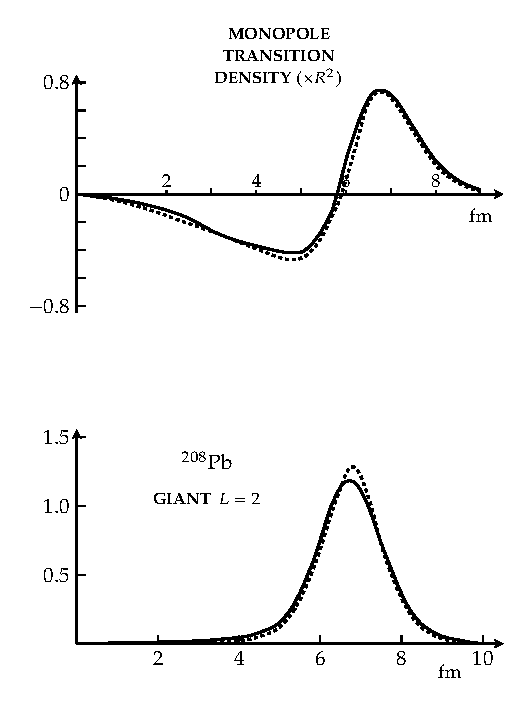
\includegraphics[width=0.8\textwidth]{pictures/8_14}
\par\end{centering}
\caption{\label{fig:8_14}$^{208}\mathrm{Pb}$ 中的同位旋标量单极与四极跃迁密度（引自 \cite{BT75}）。虚线为简单流体动力学公式，实线为连续谱
RPA 计算结果。}
\end{figure}

\ref{fig:8_14} 表明流体动力学公式（虚线）与自洽连续谱 RPA 计算（实线）展现出惊人的吻合，这无可辩驳地证实了巨共振在本质上对应着经典核液滴的表面振动与体压缩振动。

一个典型的例子是 $^{208}\mathrm{Pb}$ 中的低激发集体 $3^{-}$ 态。\ref{fig:8_15} 展示了其实验与理论的径向跃迁密度
$\rho^{0}(r)$。实验测量值与 Bohr-Tassie 模型的宏观预测存在相当剧烈的偏离。而通过求解包含密度依赖有效力的微观
RPA 方程所得到的理论曲线，与实验数据达成了极其优良的吻合。对于高激发的 $3^{-}$ 巨八极共振，其与 Bohr-Tassie
模型的吻合则再次恢复良好［St 79］。

\begin{figure}[H]
\begin{centering}
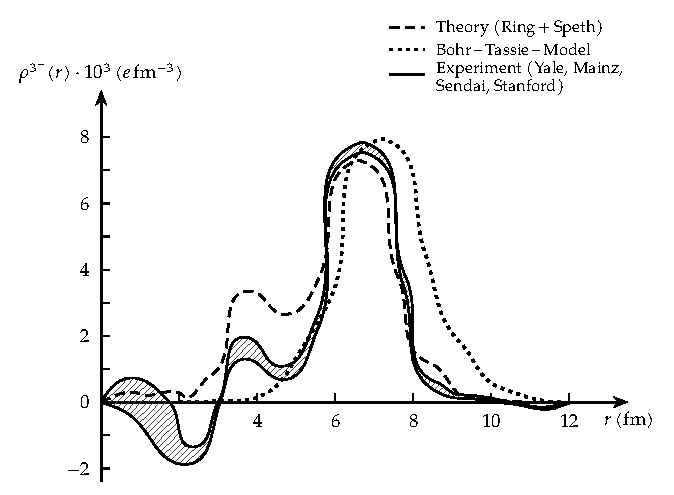
\includegraphics[width=0.7\textwidth]{pictures/8_15}
\par\end{centering}
\caption{\label{fig:8_15}$^{208}\mathrm{Pb}$ 最低 $3^{-}$ 态的理论与实验径向跃迁密度。实线标示了实验误差范围［RFM
74］，虚线［TW 73］基于采用 Migdal 力的 RPA 计算，点线对应于 Bohr-Tassie 模型（引自 \cite{St79}）。}
\end{figure}


\section{粒子-粒子 RPA\label{sec:8.8_=007C92=005B50-=007C92=005B50_RPA}}

\subsection{形式理论\label{subsec:8.8.1_=005F62=005F0F=007406=008BBA}}

正如在 Tamm-Dancoff 方法中我们区分粒子-空穴与粒子-粒子 TDA（第 8.2.3 节）一样，对应于 ph RPA，我们同样拥有粒子-粒子（pp）RPA。对于
$A+2$ 系统的本征态 $|\tau\rangle$，类比于 ph 拟设 (\ref{eq:rpa_creation_operator})，我们有：

\begin{equation}
|A+2,\tau\rangle=R^{\dagger}_{\tau}|A,0\rangle\label{eq:pprpa_state_ansatz}
\end{equation}

属于 $A$ 体系的基态由下式定义：

\begin{equation}
R_{\tau}|A,0\rangle=0\label{eq:pprpa_vacuum_def}
\end{equation}

在与式 (\ref{eq:rpa_xy_amplitudes_density}) 相同的准玻色子近似下，我们得到：

\begin{align}
X^{\tau}_{mn} & =\langle A,0|a_{n}a_{m}|A+2,\tau\rangle,\nonumber \\
Y^{\tau}_{ij} & =\langle A,0|a_{j}a_{i}|A+2,\tau\rangle\label{eq:pprpa_amplitudes_def}
\end{align}

利用 $R^{\dagger}_{\tau}$ 的运动方程，完全类比于 ph 情形（第 8.4.1 节），我们导出 $A+2$
核系统相对于 $A$ 核基态的激发能 $\hbar\Omega_{\tau}=E^{A+2}_{\tau}-E^{A}_{0}$
所满足的方程［FIS 64, Sch 64b, MLE 67, Ro 68a, b, RP 69］：

\begin{equation}
(\hbar\Omega_{\tau}-\epsilon_{m}-\epsilon_{n})X^{\tau}_{mn}=\sum_{m'<n'}\bar{v}_{mnm'n'}X^{\tau}_{m'n'}+\sum_{i'<j'}\bar{v}_{mni'j'}Y^{\tau}_{i'j'}\label{eq:pprpa_plus2_eq}
\end{equation}

对于 $A-2$ 粒子系统，我们同样得到完全对应的方程：

\begin{equation}
(\hbar\Omega_{\lambda}+\epsilon_{i}+\epsilon_{j})Y^{\lambda}_{ij}=-\sum_{i'<j'}\bar{v}_{iji'j'}Y^{\lambda}_{i'j'}-\sum_{m'<n'}\bar{v}_{ijm'n'}X^{\lambda}_{m'n'}\label{eq:pprpa_minus2_eq}
\end{equation}

式中 $\hbar\Omega_{\lambda}=E^{A}_{0}-E^{A-2}_{\lambda}$。由此，我们可以将方程
(\ref{eq:pprpa_plus2_eq}) 与 (\ref{eq:pprpa_minus2_eq}) 合并为一个类似于
ph 形式的紧凑矩阵方程：

\begin{equation}
\begin{pmatrix}A & B\\
B^{\dagger} & C
\end{pmatrix}\begin{pmatrix}X^{\tau}\\
Y^{\tau}
\end{pmatrix}=\hbar\Omega_{\tau}\begin{pmatrix}1 & 0\\
0 & -1
\end{pmatrix}\begin{pmatrix}X^{\tau}\\
Y^{\tau}
\end{pmatrix}\label{eq:pprpa_matrix_eq}
\end{equation}

式中（$m<n,\,m'<n',\,i<j,\,i'<j'$）：

\begin{align}
A_{mnm'n'} & =(\epsilon_{m}+\epsilon_{n})\delta_{mm'}\delta_{nn'}+\bar{v}_{mnm'n'},\nonumber \\
C_{iji'j'} & =-(\epsilon_{i}+\epsilon_{j})\delta_{ii'}\delta_{jj'}-\bar{v}_{iji'j'},\nonumber \\
B_{mnij} & =\bar{v}_{mnij}\label{eq:pprpa_matrix_blocks}
\end{align}

需要指出的是，Hermitian 矩阵 $A$ 与 $C$ 通常具有不同的维度，矩阵 $B$ 因而是一个长方阵。方程 (\ref{eq:pprpa_matrix_eq})
同时给出了 $A+2$ 与 $A-2$ 系统的本征态，这与 ph 情形不同（在 ph 情形中所有解属于相同粒子数的系统）。然而，这并不意味着
pp RPA 破坏了粒子数守恒（如 BCS 模型所做的那样），拟设 (\ref{eq:pprpa_state_ansatz}) 严格保持粒子数。在实践中，我们可以根据波函数的振幅特征识别出属于
$A+2$ 体系的解：它们具有很大的 pp 分量 $X_{mn}$ 与极小的 hh 分量 $Y_{ij}$，能量位于 $\epsilon_{m}+\epsilon_{n}$
能区。

pp-RPA 本征矢满足如下归一化与完备性关系：

\begin{equation}
\sum_{m<n}X^{\tau*}_{mn}X^{\tau'}_{mn}-\sum_{i<j}Y^{\tau*}_{ij}Y^{\tau'}_{ij}=\delta_{\tau\tau'}\label{eq:pprpa_orthonormality}
\end{equation}

\begin{equation}
\sum_{\tau}\left(X^{\tau}_{mn}X^{\tau*}_{m'n'}-Y^{\tau}_{mn}Y^{\tau*}_{m'n'}\right)=\delta_{mm'}\delta_{nn'}\label{eq:pprpa_closure}
\end{equation}


\subsection{对振动诱发的基态关联\label{subsec:8.8.2_=005BF9=00632F=0052A8=008BF1=0053D1=007684=0057FA=006001=005173=008054}}

利用 Thouless 定理，pp RPA 基态同样可表示为指数形式：

\begin{equation}
|\text{RPA}\rangle=N_{0}\exp\left(\sum_{m<n,\,i<j}Z_{mnij}A^{\dagger}_{mn}A_{ij}\right)|\text{HF}\rangle\label{eq:pprpa_ground_state_correlated}
\end{equation}

式中 $A^{\dagger}_{mn}=a^{\dagger}_{m}a^{\dagger}_{n}$，$A_{ij}=a_{j}a_{i}$，且
$Z=Y^{*}X^{*-1}$。展开式 (\ref{eq:pprpa_ground_state_correlated}) 可以看出，关联基态除
$|\text{HF}\rangle$ 外还包含了带有成对玻色子的虚激发，由于 pp 玻色子数目严格等于 hh 玻色子数目，粒子数是严格守恒的。

对于纯配对力 $-G$，式 (\ref{eq:pprpa_matrix_eq}) 导出如下色散关系：

\begin{equation}
\frac{2}{G}=\sum_{n}\frac{2j_{n}+1}{2\epsilon_{n}-\hbar\Omega}+\sum_{i}\frac{2j_{i}+1}{2|\epsilon_{i}|+\hbar\Omega}\label{eq:pprpa_pairing_dispersion}
\end{equation}

当配对力常数 $G$ 增大至临界值：

\begin{equation}
G_{\text{crit}}=\frac{2}{\sum_{n}\frac{2j_{n}+1}{2\epsilon_{n}}+\sum_{i}\frac{2j_{i}+1}{2|\epsilon_{i}|}}\label{eq:pprpa_gcrit_def}
\end{equation}

时，最低集体对振动的激发能 $\hbar\Omega\to0$，标志着正常核系统发生向超流态（BCS 凝聚）的相变。在 $G>G_{\text{crit}}$
时，BCS 能隙方程具有非零解 $\Delta>0$，此时必须采用准粒子表象。

\section{准粒子 RPA（QRPA）\label{sec:8.9_=0051C6=007C92=005B50RPA=00FF08QRPA=00FF09}}

在远离闭壳层时，配对关联极其重要，使得配对场对单粒子运动的反馈不再能够忽略。我们在第 6 章和第 7 章已经看到，在这些情形下，采用
BCS 或 HFB 基态是恰当的。由于它也是一个广义行列式波函数，我们可以完全类比于正常系统构造 TDA 和 RPA 理论［Ba 60a］。由此将显现出：粒子-空穴
RPA 与粒子-粒子 RPA 可以被统一包容于一个紧凑的准粒子 RPA（QRPA）方程之中［So 71］。

为了推导这些方程，我们从准粒子表象下的 Hamiltonian 量［式 (E.18)］出发：

\begin{equation}
H=H^{0}+H^{11}+H^{20}+H^{40}+H^{31}+H^{22}\label{eq:qrpa_h_quasiparticle_decomp}
\end{equation}

准粒子声子算符定义为：

\begin{equation}
Q^{\dagger}_{\nu}=\sum_{k<k'}\left(X^{\nu}_{kk'}\alpha^{\dagger}_{k}\alpha^{\dagger}_{k'}-Y^{\nu}_{kk'}\alpha_{k'}\alpha_{k}\right)\label{eq:qrpa_phonon_creation_def}
\end{equation}

类比于第 8.4.1 节的推导，我们得到准粒子 RPA 方程，其矩阵形式与式 (\ref{eq:rpa_matrix_equation})
完全一致：

\begin{equation}
\begin{pmatrix}A & B\\
B^{*} & A^{*}
\end{pmatrix}\begin{pmatrix}X^{\nu}\\
Y^{\nu}
\end{pmatrix}=\hbar\Omega_{\nu}\begin{pmatrix}1 & 0\\
0 & -1
\end{pmatrix}\begin{pmatrix}X^{\nu}\\
Y^{\nu}
\end{pmatrix}\label{eq:qrpa_matrix_equation}
\end{equation}

唯独此时矩阵指标遍历组态空间中的所有准粒子对 $(k<k')$。矩阵 $A$ 和 $B$ 给定为（$k<k',\,l<l'$）：

\begin{align}
A_{kk'll'} & =\langle\text{HFB}|[\alpha_{k'}\alpha_{k},[H,\alpha^{\dagger}_{l}\alpha^{\dagger}_{l'}]]|\text{HFB}\rangle=(E_{k}+E_{k'})\delta_{kl}\delta_{k'l'}+H^{22}_{kk'll'},\nonumber \\
B_{kk'll'} & =-\langle\text{HFB}|[\alpha_{k'}\alpha_{k},[H,\alpha_{l'}\alpha_{l}]]|\text{HFB}\rangle=H^{40}_{kk'll'}\label{eq:qrpa_ab_matrices_def}
\end{align}

它们共同构成了 HFB 理论的稳定性矩阵［式 (7.37)］。在时间反演不变的规范基下，矩阵元可以利用 Bogoliubov 变换的
$u,v$ 系数显式计算：

\begin{align}
A_{kk'll'} & =(E_{k}+E_{k'})\delta_{kl}\delta_{k'l'}+\bar{v}_{kl'k'l}(u_{k}v_{k'}u_{l}v_{l'}+v_{k}u_{k'}v_{l}u_{l'})+\cdots,\nonumber \\
B_{kk'll'} & =\bar{v}_{kk'll'}(u_{k}u_{k'}v_{l}v_{l'}+v_{k}v_{k'}u_{l}u_{l'})+\cdots\label{eq:qrpa_uv_coefficients_explicit}
\end{align}

在 Hartree-Fock 极限下（所有 $u=0,1$），QRPA 方程自动退化并解耦为通常的粒子-空穴 RPA 方程与粒子-粒子
RPA 方程。

准粒子 RPA 方程已广泛应用于结合可分离相互作用（如配对加四极模型、表面 $\delta$ 相互作用）的研究中。它不仅能够成功描述球形超导核中的低激发集体振动，而且能够成功应用于形变稀土核和锕系核中
$\beta$ 振动、$\gamma$ 振动、八极振动以及配对振动的微观描述；同时通过结合推转自洽模型，亦能很好地描述伴随其上的转动带结构与形变核中的巨共振现象。



\chapter{玻色展开方法\label{chap:=0073BB=008272=005C55=005F00=0065B9=006CD5}}

\section{引言\label{sec:9.1_=005F15=008A00}}

在上一章中，我们在简谐近似下研究了原子核的集体振动。简谐振动的显著特征是具有等间距的能谱。如图 1.5 所示，在四极振动情形下，我们预期在激发能量为
$2\hbar\omega$ 处存在一个三度简并的三重态（$0^{+}$、$2^{+}$、$4^{+}$），而在三倍能量 $3\hbar\omega$
处存在一个由五重能级（$0^{+}$、$2^{+}$、$3^{+}$、$4^{+}$、$6^{+}$）组成的多重态。在实际核谱中，许多近球形核的低激发态确实相当清晰地展现出这种多声子结构。然而，若仔细考查细节，人们总会发现实际能谱或多或少、乃至剧烈地偏离这种纯简谐图像，例如高阶多重态的能级发生劈裂，以及多重态能量重心的整体移动。

导致这些非谐效应（anharmonicities）的原因主要来自两种效应：
\begin{enumerate}
\item 集体费米子对算符\footnote{为了简便起见，在本章引言中我们使用粒子-空穴（ph）表象。在此表象中，算符 $a^{\dagger}_{m}$ 产生一个粒子，而
$a_{i}$ 产生一个空穴（参见第 8 章）。如果考虑超流核，则应相应地引入准粒子（见第 7 章）。}
\begin{equation}
b^{\dagger}=\sum_{mi}C_{mi}a^{\dagger}_{m}a_{i}\label{eq:9.1}
\end{equation}
并不是严格意义上的理想玻色子。当我们为了描述双声子态而两次作用该产生算符时，所得到的并不是两个彼此解耦的理想玻色子，因为 Pauli
原理排除了任何可能使相同能级被一个以上粒子（或空穴）所占据的组态。我们将这类源于反对称性基底与态空间限制的效应称为\textbf{运动学效应}（kinematic
effects），它们在后文各节中将与所采用的展开基底密切相关。
\item 精确的多体 Hamiltonian 不仅包含在 TDA 近似（或 RPA 方法）中被对角化的玻色子二次项，而且还包含更高阶的非线性项。这些高阶相互作用项在纯简谐近似下被忽略掉了，它们不仅在不同的集体振动模式之间引入了非谐耦合，而且还提供了集体模式与非集体态（例如近乎纯粹的双准粒子态）之间的耦合通道。我们将这类由体系多体相互作用性质决定的效应称为\textbf{动力学效应}（dynamic
effects）。
\end{enumerate}
如果我们从具有相当纯粹简谐振动谱的双幻核出发，逐步向核中添加越来越多的价核子，就会观察到越来越强烈的非谐效应。体系随之进入过渡区核（transitional
nuclei），在这一区域中，能谱的纯振动特征逐渐瓦解，转动能带结构开始孕育并发展起来。最终，当离开闭壳层足够远时，体系演化为具有良好变形特征的稳定形变核，并呈现出优美的纯转动带谱。

借助本章所讨论的方法，我们原则上有能力微观地描述这种非谐性演化，乃至描述向形变核的相变过渡。这些方法的核心基本思想，在于将原始的费米子
Hamiltonian 严格或近似地用纯玻色子产生和湮灭算符 $B^{\dagger}_{\mu}$、$B_{\mu}$ 来表达，并在相应的玻色子态空间中对其进行对角化。在数学上，这对应于将多费米子态的
Fock 空间映射到一个理想玻色子态空间中。这将在 \ref{sec:9.2_=005076=005076=006838=004E2D=007684=0073BB=008272=005B50=008868=008C61}
中予以详尽阐述。

采用这种玻色子表象的显著优势在于：高度集体的激发模式——例如四极集体振动模式——能够用形式上极为简单的波函数来近似表示，即单玻色子态
$B^{\dagger}_{\mu}|0)$。正如我们在上一章中所见，对于这类集体态，Hamiltonian 的二次玻色子近似已经相当优良。因此我们完全有理由期望，Hamiltonian
在玻色子表象中的高阶展开项将会迅速衰减。在 \ref{sec:9.2_=005076=005076=006838=004E2D=007684=0073BB=008272=005B50=008868=008C61}
中我们将看到，对于集体激发模式而言事实确乎如此：通常只需计及四阶或六阶玻色子展开项就足以给出极高的计算精度。

另一方面，描述非集体激发模式所必需的纯粒子-空穴算符 $a^{\dagger}_{m}a_{i}$ 在玻色子空间中则具有相当繁复的展开结构。因此，各种玻色展开方法的核心主旨，在于将我们自身严格限制在少数几个集体玻色子所张成的有限子空间（即全
Hilbert 空间的集体子空间）之内，并在此集体子空间中对有效 Hamiltonian 进行对角化。只要精确多体 Hamiltonian
的低激发本征态大体落在此子空间内，亦即只要我们能够合理地忽略它们与 Hilbert 空间中其余非集体态之间的耦合，便能够以极为简练的物理图象和数学形式实现对这些态的描述。

当然，这一假设绝不可能对所有的核态或所有的原子核都严格成立。在许多实际核物理问题中，我们必须显式地计及集体模式与非集体的少数准粒子态之间的动力学耦合。对于奇质量核（奇
A 核）系统而言，情形尤为如此。因此，在 \ref{sec:9.3_=005947A=006838=004E0E=007C92=005B50-=00632F=0052A8=008026=005408}
中，我们将专门讨论处理集体模式（在玻色子图象下描述）与单粒子自由度之间相互耦合的技术。这类模型中最具代表性且最简明优美的范例，当属由
Bohr 和 Mottelson 所建立的粒子-振动耦合（particle vibration coupling, PVC）模型。

\section{偶偶核中的玻色子表象\label{sec:9.2_=005076=005076=006838=004E2D=007684=0073BB=008272=005B50=008868=008C61}}

\subsection{角动量算符的玻色子表象\label{subsec:9.2.1_=0089D2=0052A8=0091CF=007B97=007B26=007684=0073BB=008272=005B50=008868=008C61}}

用玻色子算符来表示费米子体系的问题已经在物理学的众多分支领域中得到了广泛而深入的研究（文献综述参见 \cite{Ga78}）。由于这类表象方法通常具有高度抽象的数学形式，因此在本节中，我们首先从几个简明的物理例子出发，它们已经能够充分展示此类方法的基本特征与核心概念。

角动量算符本身就可以用玻色子来精确表示。在铁磁体自旋波理论中，人们已经发展出了数种此类技巧，并且事实证明，其中的一部分方法能够自然地推广到一般的多费米子体系。

我们首先考虑角动量算符 $J_{\pm}=J_{x}\pm\mathrm{i}J_{y}$ 与 $J_{z}$ 所构成的 Lie
代数，它们满足群 $SU(2)$ 的对易关系：
\begin{equation}
[J_{+},J_{-}]=2J_{z},\qquad[J_{z},J_{\pm}]=\pm J_{\pm}.\label{eq:9.2}
\end{equation}
相应的 Hilbert 空间由 $J^{2}$ 与 $J_{z}$ 的共同本征矢 $|IM\rangle$ 所张成。现在我们将这一
Hilbert 空间映射到一个由玻色子真空\footnote{在下文中，我们一律用尖括号 $|\;\rangle$ 表示原始的角动量态与费米子态，而用圆括号 $|\;)$ 表示玻色子空间中的态矢。}$|0)$
以及满足下列代数关系的玻色子产生和湮灭算符 $B^{\dagger},B$ 所定义的玻色子空间：
\begin{equation}
[B,B^{\dagger}]=1,\qquad B|0)=0.\label{eq:9.3}
\end{equation}
实现这种映射（即将算符 $J_{i}$ 用玻色子算符 $B,B^{\dagger}$ 来表达）的方式有多种：
\begin{enumerate}
\item \textbf{Holstein-Primakoff 表象} \cite{HP40}：将讨论限制在由固定角动量量子数 $I$ 所表征的子空间中，我们可以按如下方式映射算符
$J_{\pm}$ 与 $J_{z}$：
\begin{align}
J_{+}\to(J_{+})_{B} & =\sqrt{2I}B^{\dagger}\sqrt{1-\frac{1}{2I}B^{\dagger}B},\nonumber \\
J_{-}\to(J_{-})_{B} & =\left[(J_{+})_{B}\right]^{\dagger}=\sqrt{2I}\sqrt{1-\frac{1}{2I}B^{\dagger}B}\,B,\label{eq:9.4}\\
J_{z}\to(J_{z})_{B} & =-I+B^{\dagger}B.\nonumber 
\end{align}
这里的平方根符号形式上代表其相应的 Taylor 级数展开。容易直接验证，玻色子空间中的算符 $(J_{\pm})_{B}$ 与
$(J_{z})_{B}$ 严格满足角动量代数 \ref{eq:9.2}。

全玻色子空间由 $n$-玻色子态所张成：
\begin{equation}
|n)=\frac{1}{\sqrt{n!}}(B^{\dagger})^{n}|0),\qquad n=0,1,2,\ldots\label{eq:9.5}
\end{equation}
与具有有限维数 $2I+1$ 的角动量子空间不同，玻色子空间的维数是无限的（$n\to\infty$）。另一方面，由于 $B^{\dagger}B$
计算玻色子的数目 $n$，式 \ref{eq:9.4} 中的平方根在全玻色子空间中并非处处有定义。因此我们必须施加条件：
\begin{equation}
n\le2I.\label{eq:9.6}
\end{equation}
在无穷维玻色子空间中，最多仅包含 $2I$ 个玻色子的子空间被称为\textbf{物理子空间}（physical subspace）。它由
$2I+1$ 个基矢
\begin{equation}
|0),\;B^{\dagger}|0),\;\ldots,\;(B^{\dagger})^{2I}|0)\label{eq:9.7}
\end{equation}
所张成，因而与原始角动量空间具有完全相同的维数。映射 \ref{eq:9.4} 在由 $I$ 表征的角动量空间与物理子空间之间建立了一一对应关系。由于该映射严格保持了对易关系不变，因此在哪个空间中进行实际计算纯粹取决于计算上的便利性。体系所有具有物理重要性的性质在该映射下均保持不变。

这正是所有玻色子表象方法的核心思想。在此我们已经清楚地看到，要使这一概念成立，必须满足两项基本要素：
\begin{enumerate}
\item 必须确保计算中的代数规则——即底层的算符代数——在映射过程中严格守恒。
\item 只允许在物理子空间内开展计算，即在我们的例子中，所有态矢量都必须属于算符 $J^{2}$ 对应于本征值 $I(I+1)$ 的本征子空间。一般而言，这一事实可以表述为：人们只能使用那些属于底层对称性群的
Casimir 算符的本征态的矢量 \cite{Ya74}。
\end{enumerate}
作为具体示例，我们可以将角动量本征态用玻色子态显式表示为：
\begin{equation}
|IM\rangle\to|IM)=\left[(I+M)!\right]^{-1/2}(B^{\dagger})^{I+M}|0).\label{eq:9.8}
\end{equation}
在实际应用中，我们必须对式 \ref{eq:9.4} 采用 Taylor 展开。当玻色子数目相对于 $2I$ 而言很小时，展开收敛极快。此类玻色子表象的一个不可避免的缺点在于：原则上需要无穷多阶展开项才能严格满足对易代数
\ref{eq:9.2}。然而，还存在着其他途径来避开这一困难：
\item \textbf{Dyson 表象} \cite{Dy56}：Dyson 提出了如下映射形式：
\begin{align}
J_{+}\to(J_{+})_{B} & =\sqrt{2I}B^{\dagger}\left(1-\frac{1}{2I}B^{\dagger}B\right),\nonumber \\
J_{-}\to(J_{-})_{B} & =\sqrt{2I}B,\label{eq:9.9}\\
J_{z}\to(J_{z})_{B} & =-I+B^{\dagger}B.\nonumber 
\end{align}
这种表象形式极为简练，其展开在有限阶截断，但它破坏了 Hermite 性，因为 $(J_{+})^{\dagger}_{B}$ 不等于
$(J_{-})_{B}$，从而导致非 Hermite 的有效 Hamiltonian。然而正如我们在后文各节中所见，它具有独特的显著优势，并且同样能够成功应用于核多体问题。
\item \textbf{Schwinger 表象} \cite{Sch65}：Schwinger 引入了一种不仅有限截断、而且完全保持 Hermite
性的角动量算符玻色子表象。他引入了两种独立的玻色子算符 $A$ 与 $B$：
\begin{equation}
[A,A^{\dagger}]=1,\qquad[B,B^{\dagger}]=1,\qquad[A,B]=[A,B^{\dagger}]=0,\label{eq:9.10}
\end{equation}
它们作用在二维谐振子态空间中：
\begin{equation}
|n_{A},n_{B})=\frac{1}{\sqrt{n_{A}!n_{B}!}}(A^{\dagger})^{n_{A}}(B^{\dagger})^{n_{B}}|0,0).\label{eq:9.11}
\end{equation}
Schwinger 表象的具体定义为：
\begin{align}
J_{+}\to(J_{+})_{B} & =B^{\dagger}A,\nonumber \\
J_{-}\to(J_{-})_{B} & =(J_{+})^{\dagger}_{B}=A^{\dagger}B,\label{eq:9.12}\\
J_{z}\to(J_{z})_{B} & =\frac{1}{2}(B^{\dagger}B-A^{\dagger}A).\nonumber 
\end{align}
角动量算符的共同本征态在此表象下可以写成：
\begin{equation}
|IM)=\left[(I-M)!(I+M)!\right]^{-1/2}(B^{\dagger})^{I+M}(A^{\dagger})^{I-M}|0,0).\label{eq:9.13}
\end{equation}
在此表象中，总玻色子数算符
\begin{equation}
N=B^{\dagger}B+A^{\dagger}A=2I\label{eq:9.14}
\end{equation}
正比于总角动量量子数 $I$。因此，任何转动不变的 Hamiltonian 都必须严格守恒该总玻色子数。这与 Holstein-Primakoff
表象形成了鲜明对比，后者会产生破坏玻色子数守恒的项。另一方面，可以证明在两种表象之间存在着近乎单一的么正变换 \cite{BM78}。
\end{enumerate}
当 Hamiltonian 可以用自旋或准自旋算符表示时（例如 Lipkin 模型，参见 \ref{sec:5.4_Lipkin=006A21=00578B}；或
Seniority 模型，参见 \ref{sec:6.2_Seniority=0065B9=006848}），角动量算符的玻色子表象便能直接派上用场。在这些情形中，我们能够立即得到
Hamiltonian 的玻色子表象。正因如此，这些模型被广泛用于深入研究各种玻色子表象的性质 \cite{PKD68,BS68b,KI69}，我们将在后文各节中重访其中的一些模型。

角动量算符的玻色子表象也已被应用于转子模型中（参见 \ref{sec:1.5_=008F6C=0052A8=005E26}）。Marshalek
\cite{Ma75b} 引入了式 \ref{eq:9.4} 的推广形式，其中包含对应于通常由 Euler 角所描述的三个转动自由度的三个玻色子。Yamamura
等人 \cite{YSI78,IY78} 则采用了 Schwinger 表象的推广。这些方法在大角动量极限下最为有效，此时体系基本表现为绕某一固定轴的经典转动。在玻色子图象下，偏离该定轴转动的微小偏离可被描述为转动轴的微小摆动，即所谓摇摆玻色子（wobbling
bosons）\cite{BM75,Ma79}。

\subsection{玻色展开的概念\label{subsec:9.2.2_=0073BB=008272=005C55=005F00=007684=006982=005FF5}}

在上一小节中，我们讨论了角动量算符玻色子表象的若干经典范例。这些方法均可自然推广至多费米子体系。我们首先将讨论局限在具有偶数核子数的体系中；奇数体系将在
\ref{sec:9.3_=005947A=006838=004E0E=007C92=005B50-=00632F=0052A8=008026=005408}
中予以专门处理。

所有这些方法都始于一个包含态矢与算符的多费米子 Hilbert 空间 $\mathcal{H}_{F}$。在二次量子化表述中，该空间完全由费米子真空
$|0\rangle$ 以及一组费米子产生算符 $\alpha^{\dagger}_{k}$ 所确定。在下文中，我们始终在准粒子图象下工作，即算符
$\alpha^{\dagger}_{k}$ 是第 7 章意义下的 Bogoliubov 准粒子算符；Hartree-Fock（HF）准粒子仅仅是其在无配对关联时的特例。

由于玻色子具有整数自旋，我们更倾向于采用费米子对算符：
\begin{equation}
\alpha^{\dagger}_{k}\alpha^{\dagger}_{l},\qquad\alpha_{l}\alpha_{k},\qquad\alpha^{\dagger}_{k}\alpha_{l}.\label{eq:9.15}
\end{equation}
事实上，偶数体系中的所有波函数和物理算符均可完全用这些费米子对以及相应的准粒子真空 $|0\rangle$ 来描述\footnote{若从对应于奇数系统的真空 $|0\rangle$ 出发，原则上也同样能够描述奇数系统（参见 \ref{sec:9.3_=005947A=006838=004E0E=007C92=005B50-=00632F=0052A8=008026=005408}）。}。

现在，将该费米子空间映射到另一个不同的 Hilbert 空间——即玻色子空间 $\mathcal{H}_{B}$：
\begin{equation}
\mathcal{H}_{F}\to\mathcal{H}_{B}.\label{eq:9.16}
\end{equation}
玻色子空间 $\mathcal{H}_{B}$ 由玻色子真空 $|0)$ 以及玻色子产生和湮灭算符 $B^{\dagger}_{\mu},B_{\mu}$
所定义\footnote{在非集体情形下，玻色子指标 $\mu$ 对应于一个费米子对 $(k,l)$。}：
\begin{equation}
B_{\mu}|0)=0,\qquad[B_{\mu},B^{\dagger}_{\nu}]=\delta_{\mu\nu},\qquad[B_{\mu},B_{\nu}]=0.\label{eq:9.17}
\end{equation}
正如角动量情形（\ref{subsec:9.2.1_=0089D2=0052A8=0091CF=007B97=007B26=007684=0073BB=008272=005B50=008868=008C61}）一样，通常玻色子空间
$\mathcal{H}_{B}$ 远大于费米子空间 $\mathcal{H}_{F}$。因此，映射 \ref{eq:9.16}
仅在玻色子空间的某一确定子空间 $\mathcal{H}_{\text{phys}}$ 内才是单射且单值的：
\[
\mathcal{H}_{F}\to\mathcal{H}_{\text{phys}}\subset\mathcal{H}_{B}.
\]
显式引入这一映射\footnote{除了此处所讨论的两种主要概念外，还存在着其他映射方式，例如 \ref{subsec:9.2.5_Dyson=0073BB=008272=005C55=005F00}
中所讨论的 Dyson 映射。}的基本方案主要有两种：
\begin{enumerate}
\item \textbf{Belyaev 与 Zelevinski 方案} \cite{BZ62}：主张以保持算符对易关系的方式来映射物理算符。通常，所有重要的物理算符均可由一组基础算符构成，这些基础算符的对易子构成一个封闭的
Lie 代数。式 \ref{eq:9.15} 的算符集合便是一个典型示例；另一个例子是 Lipkin 模型（\ref{sec:5.4_Lipkin=006A21=00578B}）中的准自旋算符
$K_{\pm},K_{0}$。因此，只需将这些基础算符映射到玻色子空间中的算符上，使得原先的代数关系得以严格保持即可。\footnote{原则上，人们也可以要求保留反对易关系 \cite{Am65,DK75}。然而，由于反对易子在玻色子表象中通常很难精确处理，因此在实际中该方案很少被采用。}所有其他物理算符均可表达为这些基础算符的多项式，而在玻色子空间中的对应像，只需将多项式中的基础算符替换为其相应的玻色子像即可。

为了获得态矢量的映射，人们只需在玻色子真空 $|0)$ 与费米子准粒子真空 $|0\rangle$ 之间建立对应关系。所有激发态均可通过基础算符的相继作用而获得。显然，通过这种方式生成的态矢并不能张满整个玻色子空间，而仅仅张成了物理子空间。正如引言所指出的，物理子空间是相应对易代数的
Casimir 算符的本征子空间。当对易代数仅在近似意义下被满足时，便可能混入非物理的赝态组分。为了排除这些伪成分，人们至少必须确保计算始终局限在
Casimir 算符的本征子空间之内 \cite{Ya74}。
\item \textbf{Marumori 方案} \cite{MYT64a,MYT64b}：主张直接建立 Hilbert 空间 $\mathcal{H}_{F}$
与 $\mathcal{H}_{B}$ 中态矢量的映射，并据此定义算符的映射，使得所有的矩阵元严格保持不变。在实际操作中，人们从玻色子物理子空间的一组正交归一基底出发：
\[
(n|n')=\delta_{nn'},\qquad\sum_{n}|n)(n|=1_{\text{phys}},
\]
并将它们一一映射到费米子空间中相应的归一化态 $|n\rangle$ 上。

于是，费米子空间中任意算符 $O_{F}$ 在玻色子空间中的对应像由下式给出：
\begin{equation}
O_{F}\to O_{B}=\sum_{nn'}\langle n|O_{F}|n'\rangle|n)(n'|.\label{eq:9.18}
\end{equation}
显而易见，该定义直接保证了算符矩阵元的守恒。然而，按照这一处方将费米子态 $|n\rangle$ 映射到玻色子态的过程并非自然唯一。在
\ref{subsec:9.2.6_=006570=005B66=0080CC=00666F} 中，我们将详细探讨如何通过严格限制在物理子空间内以唯一确定的方式实现这一映射。
\end{enumerate}
上述两种映射算符（Belyaev-Zelevinski）或映射态矢量（Marumori）的概念在文献中已经得到了多种不同方式的应用。在深入讨论具体方法之前，我们必须强调：在所有的实际核物理应用中，我们都不可避免地需要采用或大或小程度的激进近似，这些近似只有在特定的物理情形下才具有正当性。例如，将式
\ref{eq:9.4} 截断为仅包含有限项的 Taylor 级数展开，只有在角动量 $I$ 很大时才具有良好意义，即 $J_{+}$
本身已经展现出非常明确的玻色子特征的情形。因此，极其关键的一点是：在第一级近似下被映射到玻色子上的基础费米子算符，必须经过物理上极为审慎的选择，以确保展开具有迅速的收敛性。在纯数学上，人们完全可以从纯双准粒子算符
$\alpha^{\dagger}_{k}\alpha^{\dagger}_{l}$ 出发（参见 \ref{subsec:9.2.6_=006570=005B66=0080CC=00666F}）。然而，由于单个纯费米子对对玻色子对易关系的满足程度极差，相应的玻色展开收敛极为缓慢，在实际应用中几乎没有实用价值。

因此，只有当我们从费米子对的特定线性叠加出发时，玻色子表象才真正具有实际意义：
\begin{equation}
b^{\dagger}_{\mu}=\frac{1}{2}\sum_{kl}C^{\mu}_{kl}\alpha^{\dagger}_{k}\alpha^{\dagger}_{l},\label{eq:9.19}
\end{equation}
在后文中我们将其称为\textbf{集体费米子对算符}（collective fermion pair operators）。\footnote{有关“集体”概念的详细讨论，请参见 \ref{subsec:8.2.2_=0096C6=004F53=006027=007684=005224=00636E}。}展开系数
$C^{\mu}_{kl}=-C^{\mu}_{lk}$ 可以从 TDA 计算中获得（参见 \ref{sec:8.2_Tamm-Dancoff=008FD1=004F3C}），或者也可以采用特定对称性类型的算符，例如五个四极算符：
\begin{equation}
b^{\dagger}_{M}=\frac{1}{\sqrt{2}}\sum_{jj'mm'}C^{2M}_{jmj'm'}\alpha^{\dagger}_{jm}\alpha^{\dagger}_{j'm'}\qquad(M=-2,\ldots,+2).\label{eq:9.20}
\end{equation}
由于其优良的群论性质，它们在处理上十分简便，并在文献中得到了极其广泛的应用。然而我们必须清醒地认识到：一旦我们将给定的算符 $b^{\dagger}_{\mu}$
的数目限制为少数几个，式 \ref{eq:9.19} 的算符集合在双准粒子空间中就不再构成完备系，从而无法描述那些未被计及的状态。例如，在纯四极玻色子张成的子空间中，无论如何也不可能逼近一个纯粹的双准粒子非集体态。

迄今为止，我们都将多费米子系统的低激发集体运动视为近似玻色子，并据此构建了基于相应理想玻色子的微观理论。另一种需要处理准玻色子的体系是粒子对体系。正如我们在
\ref{subsec:9.2.7_=0057FA=004E8Epp-=0073BB=008272=005B50=007684=0065B9=006CD5}
中所见，此类方法与 Schwinger 表象的思想密切相连 {[}参见式 \ref{eq:9.12}{]}。其突出优点在于粒子数守恒等内禀对称性从一开始就得到了严格保障，但缺点在于我们必须用许多玻色子从裸真空中构建系统的基态，这在一般情形下可能是一项极为繁重的任务。

在阐明了这些总纲性概念之后，在接下来的各小节中，我们将立足于基于集体粒子-空穴（或双准粒子）态的玻色子，更加详细地讨论用于描述多费米子系统的几种主要微观方法。

\subsection{Belyaev-Zelevinski 玻色展开\label{subsec:9.2.3_Belyaev-Zelevinski=0073BB=008272=005C55=005F00}}

我们首先从多费米子空间的准粒子表象出发。该表象建立在广义 Slater 行列式 $|0\rangle$ 之上，该态充当准粒子湮灭算符
$(\alpha_{1},\ldots,\alpha_{2M})$ 的真空态。体系的微观多体 Hamiltonian 具有如下标准形式\footnote{由于假定基态 $|0\rangle$ 是变分原理（式 7.31）的自洽解，因此 $H^{20}$ 不出现。然而这一事实对于后文讨论并不构成实质性限制。}（式
E.18）：
\begin{equation}
H=H_{0}+H^{11}+H^{22}+H^{31}+H^{40}.\label{eq:9.21}
\end{equation}
在偶数体系中，只需考虑费米子对算符\footnote{在下文中，我们一律用小写拉丁字母表示费米子对算符，用大写拉丁字母表示玻色子算符。在非集体情形下标采用双粒子对指标 $(k,l)$，在集体情形下标则采用希腊字母
$\mu,\nu,\ldots$。}：
\begin{equation}
b^{\dagger}_{kl}=\alpha^{\dagger}_{k}\alpha^{\dagger}_{l}=-b^{\dagger}_{lk},\qquad b_{kl}=\alpha_{l}\alpha_{k},\qquad a_{kl}=\alpha^{\dagger}_{l}\alpha_{k}.\label{eq:9.22}
\end{equation}
这些对算符构成一个封闭的 Lie 代数（隶属于正交群 $SO(2M)$）：
\begin{align}
[b_{kl},b_{k'l'}] & =0,\label{eq:9.23a}\\{}
[b_{kl},b^{\dagger}_{k'l'}] & =\delta_{kk'}\delta_{ll'}+\delta_{kl'}a_{lk'}+\delta_{lk'}a_{kl'}-(k\leftrightarrow l),\label{eq:9.23b}\\{}
[b_{kl},a_{k'l'}] & =\delta_{ll'}b_{kk'}-(k\leftrightarrow l),\label{eq:9.23c}\\{}
[a_{kl},a_{k'l'}] & =\delta_{kl'}a_{k'l}-\delta_{lk'}a_{kl'}.\label{eq:9.23d}
\end{align}
原则上，非集体费米子对算符可以直接用相应的玻色子来表示，我们在 \ref{subsec:9.2.6_=006570=005B66=0080CC=00666F}
中将详细展示这一点。然而正如前文所述，为了满足所有的实际计算要求，我们必须采用集体玻色子。因此，我们从集体费米子对算符出发：
\begin{align}
b^{\dagger}_{\mu} & :=\sum_{k<l}C^{\mu}_{kl}\alpha^{\dagger}_{k}\alpha^{\dagger}_{l},\label{eq:9.24}\\
a_{\mu\nu} & :=\sum_{klr}C^{\mu*}_{kl}C^{\nu}_{lr}a_{kr}=a^{\dagger}_{\nu\mu}.\label{eq:9.25}
\end{align}
展开系数 $C^{\mu}_{kl}=-C^{\mu}_{lk}$ 表征了用于构建表象的玻色子物理特性。我们假定它们满足正交归一与完备性关系（式
8.26）：
\begin{equation}
\sum_{k<l}C^{\mu*}_{kl}C^{\mu'}_{kl}=\delta_{\mu\mu'},\qquad\sum_{\mu}C^{\mu}_{kl}C^{\mu*}_{k'l'}=\delta_{kk'}\delta_{ll'}-(k\leftrightarrow l).\label{eq:9.26}
\end{equation}
只要我们计及所有的 $\mu$ 值，式 \ref{eq:9.24} 就代表费米子对空间中的一个么正变换。但在实际应用中，我们往往只保留一个或少数几个玻色子，这意味着在使用完备性关系
\ref{eq:9.26} 时必须格外审慎。

现在，我们可以利用式 \ref{eq:9.24} 导出集体费米子对算符 \ref{eq:9.24} 与 \ref{eq:9.25}
的对易代数：
\begin{align}
[b_{\mu},b_{\mu'}] & =[b^{\dagger}_{\mu},b^{\dagger}_{\mu'}]=0,\label{eq:9.27a}\\{}
[b_{\mu},b^{\dagger}_{\mu'}] & =\delta_{\mu\mu'}-a_{\mu\mu'},\label{eq:9.27b}\\{}
[b_{\mu},a_{\mu'\nu'}] & =\sum_{\rho}\Gamma^{\mu\nu'}_{\mu'\rho}b_{\rho},\label{eq:9.27c}\\{}
[b^{\dagger}_{\mu},a_{\mu'\nu'}] & =-\sum_{\rho}\Gamma^{\mu'\rho}_{\nu'\mu}b^{\dagger}_{\rho},\label{eq:9.27d}\\{}
[a_{\mu\nu},a_{\mu'\nu'}] & =\frac{1}{M-2}\sum_{\rho\sigma}\left(\Gamma^{\mu'\mu\sigma}_{\nu'\nu\rho}-\Gamma^{\mu\mu'\sigma}_{\nu'\nu\rho}\right)a_{\rho\sigma},\label{eq:9.27e}
\end{align}
其中 $M$ 是单粒子位形空间的维数（该因子在最终公式中会完全消去，因此无需担忧无穷维空间的问题）。结构常数 $\Gamma^{\mu\nu}_{\mu'\nu'}$、$\Gamma^{\mu\nu\rho}_{\mu'\nu'\rho'}$
以及后文所需的其他物理量定义为：
\begin{align}
\Gamma^{\mu\nu}_{\mu'\nu'} & =\sum_{klpq}C^{\mu*}_{kl}C^{\nu'}_{lp}C^{\nu*}_{pq}C^{\mu'}_{qk},\label{eq:9.28a}\\
\Gamma^{\mu\nu\rho}_{\mu'\nu'\rho'} & =\sum_{klpqrs}C^{\mu*}_{kl}C^{\nu'}_{lp}C^{\nu*}_{pq}C^{\rho'}_{qr}C^{\rho*}_{rs}C^{\mu'}_{sk},\label{eq:9.28b}\\
\Gamma^{\mu\nu\rho\sigma}_{\mu'\nu'\rho'\sigma'} & =\ldots\nonumber \\
\Gamma^{\mu k}_{\mu'k'} & =\sum_{l}C^{\mu}_{kl}C^{\mu'*}_{k'l}.\label{eq:9.29}
\end{align}
图 9.1 直观地给出了式 \ref{eq:9.28a} 的图形表示。这些 $\Gamma$ 量与费米子对算符 $b_{\mu}$
并非真实玻色子这一事实密切相关；它们通过计及交换修正而精确体现了 Pauli 原理。利用式 \ref{eq:9.26}，我们可以证明许多有用的求和关系，例如：
\begin{align}
\sum_{\tau}\Gamma^{\tau\mu\mu'\ldots}_{\tau\nu'\ldots} & =-(M-1)\Gamma^{\mu\mu'\ldots}_{\nu'\ldots},\qquad\Gamma^{\mu}_{\nu}=-2\delta_{\mu\nu},\nonumber \\
\sum_{\tau}\Gamma^{\mu\nu}_{\mu'\tau}\Gamma^{\tau\rho}_{\nu'\rho'} & =-\Gamma^{\mu\nu\rho}_{\mu'\nu'\rho'}-\Gamma^{\mu\nu\rho}_{\mu'\rho'\nu'},\label{eq:9.30}\\
\sum_{\sigma\rho}\Gamma^{\mu\sigma}_{\nu\rho}\Gamma^{\rho\lambda}_{\sigma\tau} & =(M-2)\Gamma^{\mu\lambda}_{\nu\tau}+4\delta_{\mu\nu}\delta_{\lambda\tau},\nonumber \\
\sum_{\sigma\rho}\Gamma^{\rho l}_{\sigma k}\Gamma^{\sigma p}_{\rho q} & =(M-2)\delta_{pk}\delta_{ql}+\delta_{pq}\delta_{kl}.\nonumber 
\end{align}
为了推导式 \ref{eq:9.27a}，我们需要式 \ref{eq:9.25} 的逆关系，其形式为：
\begin{equation}
a_{kl}=\frac{1}{M-2}\left\{ \sum_{\mu\nu}\Gamma^{\nu k}_{\mu l}a_{\mu\nu}-\delta_{kl}\frac{1}{M-1}\sum_{\mu}a_{\mu\mu}\right\} ,\label{eq:9.31}
\end{equation}
将其代入式 \ref{eq:9.25} 即可直接验证。

\begin{figure}[H]
\begin{centering}
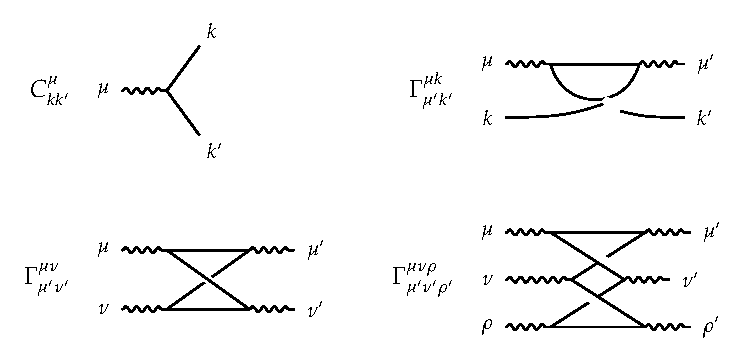
\includegraphics[width=0.8\textwidth]{pictures/9_1}
\par\end{centering}
\caption{\label{fig:9.1}物理量 $C$ 与 $\Gamma$ 的图形表示（此类图线并非附录 F 意义下的 Feynman
图）。}
\end{figure}

我们同样可以将多体 Hamiltonian（式 E.18）用集体费米子对算符 $b_{\mu}$ 与 $a_{\mu\nu}$
显式表示出来：
\begin{align}
H^{11} & =\sum_{\mu\nu}E_{\mu\nu}a_{\mu\nu},\nonumber \\
H^{22} & =\sum_{\mu\nu}V^{22}_{\mu\nu}b^{\dagger}_{\mu}b_{\nu},\label{eq:9.32}\\
H^{31} & =\sum_{\mu\nu\rho}V^{31}_{\mu\nu\rho}b^{\dagger}_{\mu}a_{\nu\rho}+\text{h.c.},\nonumber \\
H^{40} & =\sum_{\mu\nu}V^{40}_{\mu\nu}b^{\dagger}_{\mu}b^{\dagger}_{\nu}+\text{h.c.},\nonumber 
\end{align}
其中的展开矩阵元为：
\begin{align}
E_{\mu\nu} & =\frac{1}{M-2}\sum_{k}\left(\Gamma^{\nu k}_{\mu k}-\frac{1}{M-1}\delta_{\mu\nu}\right)E_{k},\nonumber \\
V^{22}_{\mu\nu} & =\frac{1}{4}\sum_{klpq}H^{22}_{klpq}C^{\mu*}_{kl}C^{\nu}_{pq},\label{eq:9.33}\\
V^{31}_{\mu\nu\rho} & =\frac{1}{M-2}\sum_{klpq}H^{31}_{klpq}C^{\mu*}_{kl}\left(\Gamma^{\rho q}_{\nu p}-\frac{1}{M-1}\delta_{\rho\nu}\delta_{pq}\right),\nonumber \\
V^{40}_{\mu\nu} & =\sum_{klpq}H^{40}_{klpq}C^{\mu*}_{kl}C^{\nu*}_{pq}.\nonumber 
\end{align}
一个具有特殊重要性的物理实例是 \textbf{Lipkin 模型}（参见 \ref{sec:5.4_Lipkin=006A21=00578B}），后文中我们还将对此进行详尽探讨。在此，我们在准粒子表象下应用该模型：算符
$\alpha^{\dagger}_{m}=c^{\dagger}_{m}$（以及 $\beta^{\dagger}_{m}=c_{-m}$）分别对应于在上能级中产生一个粒子（以及在下能级中产生一个空穴）。在
Hartree-Fock 基态 $|0\rangle$ 中，下能级（包含 $\Omega$ 个单粒子态）被完全填满：
\begin{equation}
\alpha_{m}|0\rangle=\beta_{m}|0\rangle=0.\label{eq:9.34}
\end{equation}
Hamiltonian 与准自旋算符 $\boldsymbol{K}^{2}$（式 5.47）严格对易。只要我们将讨论限制在具有本征值
$K=\Omega/2$ 的子空间中，就只有单一的集体费米子对算符（式 9.24）：
\begin{equation}
b^{\dagger}=\frac{1}{\sqrt{\Omega}}K_{+}=\frac{1}{\sqrt{\Omega}}\sum_{m}\alpha^{\dagger}_{m}\beta^{\dagger}_{m},\label{eq:9.35}
\end{equation}
其粒子-空穴振幅为 $C_{mm'}=(1/\sqrt{\Omega})\delta_{mm'}$（$m>0$）。算符 \ref{eq:9.25}
与 $K_{0}$ 紧密相连：
\begin{equation}
a=\frac{1}{\Omega}\sum_{m}\left(\alpha^{\dagger}_{m}\alpha_{m}+\beta^{\dagger}_{m}\beta_{m}\right)=1+\frac{2}{\Omega}K_{0}.\label{eq:9.36}
\end{equation}
单粒子态总数为 $M=2\Omega$，相应的 $\Gamma$ 量（式 9.28a, b）由下式给出：
\begin{equation}
\Gamma^{(2)}=+\frac{2}{\Omega},\qquad\Gamma^{(3)}=-\frac{2}{\Omega^{2}},\qquad\Gamma^{(4)}=+\frac{2}{\Omega^{3}},\quad\ldots\label{eq:9.37}
\end{equation}
此时，对易代数 \ref{eq:9.27a} 精确对应于角动量代数。以 $b$ 与 $a$ 表达的模型 Hamiltonian（式
5.45）形式为：
\begin{equation}
H=-\frac{\epsilon}{2}\Omega+\frac{\epsilon}{2}\Omega a-\frac{V}{2}\Omega(b^{\dagger}b^{\dagger}+bb).\label{eq:9.38}
\end{equation}
根据 \ref{subsec:9.2.2_=0073BB=008272=005C55=005F00=007684=006982=005FF5}
的讨论，我们本可以直接写出算符 $a$ 与 $b$ 的玻色展开；然而，我们首先希望更深入地研究一般多体情形。

依照 Belyaev 和 Zelevinski 针对一般多体情形的处理方案 \cite{BZ62}，我们首先引入一组纯理想玻色子算符：
\begin{equation}
[B_{\mu},B^{\dagger}_{\mu'}]=\delta_{\mu\mu'},\qquad[B_{\mu},B_{\mu'}]=0,\label{eq:9.39}
\end{equation}
并将费米子对算符 $b^{\dagger}_{\mu}$ 和 $a_{\mu\nu}$ 在玻色子空间中的对应像按如下方式展开\footnote{下列展开拟设显然并非唯一，但假定费米子对算符 $b^{\dagger}_{\mu}$ 的作用使玻色子数增加 1，而 $a_{\mu\nu}$
的作用不改变玻色子数，是极其合理且符合物理直觉的。}：
\begin{align}
(b^{\dagger}_{\mu})_{B} & =\sum_{\rho}x^{(1)}_{\mu\rho}B^{\dagger}_{\rho}+\sum_{\rho\nu\lambda}x^{(3)}_{\mu\nu\rho\lambda}B^{\dagger}_{\nu}B^{\dagger}_{\rho}B_{\lambda}+\cdots,\label{eq:9.40a}\\
(a_{\mu\nu})_{B} & =y^{(0)}+\sum_{\rho\lambda}y^{(2)}_{\mu\nu\rho\lambda}B^{\dagger}_{\rho}B_{\lambda}+\cdots.\label{eq:9.40b}
\end{align}
展开系数 $x^{(i)}$ 和 $y^{(i)}$ 由严格满足对易关系 \ref{eq:9.27a} 的条件唯一确定。在文献中，为了实现这一目标发展出了两种主要方法：

\subsubsection{微扰玻色展开\label{subsubsec:9.2.3.1_=005FAE=006270=0073BB=008272=005C55=005F00}}

微扰玻色展开方法建立在存在“小参数”的基础之上，对易子代数逐阶得到满足。该方法最早由 Belyaev 和 Zelevinski 提出
\cite{BZ62}，其后 Marshalek 详细研究了其数学与物理特性 \cite{Ma71,MH72,Ma74}。在那些工作中，作者们主要关注耦合到良好角动量的费米子对算符。在那种情形下，“小参数”为：
\begin{equation}
\epsilon=\frac{1}{2\bar{j}+1},\label{eq:9.41}
\end{equation}
其中 $\bar{j}$ 是 Fermi 面附近各单粒子能级的平均角动量。在实际原子核中，这一参数通常并不非常小。然而，若像式 \ref{eq:9.24}
那样处理集体费米子对，该方法的表现将大大改善。正如我们将看到的，此时的“小参数”正是式 \ref{eq:9.28a} 中的物理量
$\Gamma^{\mu\rho}_{\nu\sigma}$。如果用于展开的玻色子确实具有高度的集体性——即如果展开系数 $C^{\mu}_{kl}$
包含大量量级微小的分量——则 $\Gamma^{(2)}$ 的数值就会变得极小。Lipkin 模型便是一个典型范例 {[}参见式
\ref{eq:9.37}{]}，在那里我们有 $\Gamma^{(2)}\propto\epsilon=1/\Omega$。在这些情形下，式
\ref{eq:9.28b} 中的高阶顶点 $\Gamma^{(3)},\Gamma^{(4)}$ 均为 $\epsilon^{2},\epsilon^{3},\ldots$
的更高阶小量。

对易代数 \ref{eq:9.27a} 的满足分两步实现。首先，通过直接应用关系式 \ref{eq:9.29} 或 \ref{eq:9.30}，我们可以证明子代数
\ref{eq:9.27e} 仅通过对式 \ref{eq:9.40b} 进行有限阶展开即可精确满足：
\begin{equation}
(a_{\mu\nu})_{B}=\sum_{\rho\sigma}\Gamma^{\mu\rho}_{\nu\sigma}B^{\dagger}_{\rho}B_{\sigma},\label{eq:9.42}
\end{equation}
即 $y^{(2)}_{\mu\nu\rho\lambda}=\Gamma^{\mu\rho}_{\nu\lambda}$，而所有其他高阶系数
$y^{(n)}$ 均严格恒等于零。在下一步中，我们尝试在 $\Gamma$ 的每一微扰阶数下满足式 \ref{eq:9.27b}。零阶给出
$x^{(1)}_{\mu\rho}=\delta_{\mu\rho}$；一阶由 $x^{(3)}_{\mu\nu\rho\sigma}=-\frac{1}{4}\Gamma^{\nu\rho}_{\mu\sigma}$
满足，依此类推。经过相当冗长但直接的推导（该结果在 \ref{subsec:9.2.6_=006570=005B66=0080CC=00666F}
中可以用极其简捷的方法获得），我们最终得到无限阶微扰级数展开：
\begin{equation}
(b^{\dagger}_{\mu})_{B}=B^{\dagger}_{\mu}-\frac{1}{4}\sum_{\rho\sigma\nu}\Gamma^{\nu\rho}_{\mu\sigma}B^{\dagger}_{\nu}B^{\dagger}_{\rho}B_{\sigma}+\frac{1}{16}\sum_{\substack{\nu\rho_{1}\sigma_{1}\\
\rho_{2}\sigma_{2}
}
}\Gamma^{\nu\rho_{2}\rho_{1}}_{\mu\sigma_{1}\sigma_{2}}B^{\dagger}_{\nu}B^{\dagger}_{\rho_{1}}B_{\sigma_{1}}B^{\dagger}_{\rho_{2}}B_{\sigma_{2}}+\cdots,\label{eq:9.43}
\end{equation}
它属于式 \ref{eq:9.40a} 的形式，其系数为：
\begin{equation}
x^{(2n+1)}_{\mu\nu\rho_{1}\sigma_{1}\rho_{2}\sigma_{2}\cdots\rho_{n}\sigma_{n}}=-\frac{1}{2}\binom{1/2}{n}\Gamma^{\nu\rho_{n}\rho_{1}\rho_{2}\cdots}_{\mu\sigma_{1}\sigma_{2}\cdots\sigma_{n}}.\label{eq:9.44}
\end{equation}
我们还可以验证，该表达式在每一阶上都严格满足式 \ref{eq:9.27c} 与 \ref{eq:9.27d} 的对易关系。以此方式获得的玻色展开式相对于玻色子真空而言并非正规序（normal
order）。

在推导这些表达式的过程中，我们在许多地方使用了系数 $C^{\mu}_{kl}$ 的完备性关系 \ref{eq:9.26} 以及形如式
\ref{eq:9.30} 的求和恒等式。这意味着原则上我们必须包含所有 $\mu$ 指标及其对应的 TDA 方程（式 8.10）的解。然而在这些解中，包含了大量非集体的玻色子，对于它们而言高阶项
$\Gamma^{(n)}$ 绝不会迅速衰减。因此，只有当我们自身局限在少数几个集体玻色子（由它们所张成的空间称为\textbf{集体子空间}）之内，并且系数
$\Gamma$ 具有不将这些集体玻色子与 Hilbert 空间其余部分显著混合的特性时，整个展开才具有物理意义。例如在 Lipkin
模型中 {[}参见式 \ref{eq:9.37}{]}，$SU(2)$ 对称性保证了集体子空间的完全解耦。但在一般核多体系统中，要想找到这样一个理想解耦的集体子空间并非易事。

另一方面，要求 $\Gamma$ 不引入集体子空间与其余空间的耦合仅仅是一项\textbf{运动学条件}，它只取决于底层玻色子基底的性质。单凭这一条件尚不足以保证玻色展开的物理合理性。正如引言所指出的，只有当体系的
Hamiltonian 在集体子空间与其余 Hilbert 空间之间不产生剧烈耦合时，限制在集体子空间才是合理的，亦即集体子空间必须在良好近似下包含体系的真实物理本征态。由于这一条件直接取决于
Hamiltonian 的结构，因此被称为\textbf{动力学条件}。

基于群论对称性原因，这两项条件有时能够同时得到满足。Lipkin 模型再次为此提供了范例，在其中我们可以严格限制在具有准自旋 $\Omega/2$
的集体子空间中。此时我们只有单一的玻色子 $B$，由式 \ref{eq:9.35} 与 \ref{eq:9.42} 可得：
\begin{align}
a & =\frac{2}{\Omega}B^{\dagger}B,\nonumber \\
b^{\dagger} & =B^{\dagger}-\frac{1}{2\Omega}B^{\dagger}B^{\dagger}B-\frac{1}{8\Omega^{2}}B^{\dagger}B^{\dagger}BB^{\dagger}B-\cdots,\label{eq:9.45}
\end{align}
该级数可以精确求和为：
\begin{equation}
b^{\dagger}=B^{\dagger}\sqrt{1-\frac{1}{\Omega}B^{\dagger}B}.\label{eq:9.46}
\end{equation}
这与准自旋算符 $K_{\pm},K_{0}$ 的 Holstein-Primakoff 表象（式 9.4）完全一致。因此，Belyaev-Zelevinski
的微扰玻色展开通常也被称为 Holstein-Primakoff 展开。若我们将 Hamiltonian（式 9.38）展开至 $1/\Omega$
阶，并在正规序下排列，便得到：
\begin{equation}
H_{B}=-\frac{\epsilon}{2}\Omega+\epsilon B^{\dagger}B-V\frac{\Omega}{2}\left[\left(1-\frac{1}{2\Omega}\right)B^{\dagger}B^{\dagger}-\frac{1}{\Omega}B^{\dagger}B^{\dagger}B^{\dagger}B+\text{h.c.}\right].\label{eq:9.47}
\end{equation}
微扰玻色展开的一大显著优势在于：在最低级近似下，它严格对应于第 8.4 节中的 RPA 近似。为了看清这一点，我们采用非集体玻色子算符，并在式
\ref{eq:9.43} 中截断至第一项，即：
\[
(\alpha^{\dagger}_{k}\alpha^{\dagger}_{l})_{B}=B^{\dagger}_{kl},\qquad(\alpha^{\dagger}_{k}\alpha_{l})_{B}=\sum_{p}B^{\dagger}_{kp}B_{lp}.
\]
将这些表达式代入多体 Hamiltonian（式 E.18），并仅保留至多包含 $B^{\dagger}B,B^{\dagger}B^{\dagger},BB$
的二次项，我们便精确重现了准粒子表象（式 8.200）下的 RPA Hamiltonian（式 8.90）：
\begin{align}
H=E_{\text{HF}} & +\sum_{\substack{k<l\\
k'<l'
}
}\left\{ (E_{k}+E_{l})\delta_{kk'}\delta_{ll'}+H^{22}_{klk'l'}\right\} B^{\dagger}_{kl}B_{k'l'}\nonumber \\
 & +4\sum_{\substack{k<l\\
k'<l'
}
}\left\{ H^{40}_{klk'l'}B^{\dagger}_{kl}B^{\dagger}_{k'l'}+\text{h.c.}\right\} .\label{eq:9.48}
\end{align}
借此，我们还能以一种极为简明的方式理解为何 RPA 方法能够严格保持体系的对称性 \cite{Ma74}。由于玻色展开（式 9.43）的构建保证了在每一微扰阶数下分别独立满足对易关系，因此对于满足
\begin{equation}
[A,B]=C\label{eq:9.49}
\end{equation}
的任意两个物理算符 $A,B$，我们均有：
\begin{equation}
[A^{(n)},B^{(1)}]+[A^{(n-1)},B^{(2)}]+\cdots+[A^{(1)},B^{(n)}]=C^{(n-1)},\label{eq:9.50}
\end{equation}
其中 $A^{(n)},B^{(n)},C^{(n)}$ 分别是算符 $A,B,C$ 的玻色子部分中包含 $n$ 个 $B$
或 $B^{\dagger}$ 算符的 $n$ 阶展开项。对于与 $H$ 对易的对称性算符 $P$，从式 \ref{eq:9.50}
在 $n=2$ 时\footnote{项 $H^{(1)}$ 对应于式 7.36 中的 $H^{20}$，已被假定为零。}可得：
\begin{equation}
[H^{(2)},P^{(1)}]=0,\label{eq:9.51}
\end{equation}
这正是零频模式 $P^{(1)}$ 所满足的 RPA 方程（式 8.104）。这一论证可以平庸地推广到玻色展开的高阶项。然而，该优势在实际中的实用性受到如下事实的限制：它只有在对易代数得到精确满足时才严格成立；在更高阶展开中，我们通常需要引入截断至少数集体玻色子等激进近似，这往往会破坏对称性的严格守恒。

在数学结构上，玻色子的 RPA Hamiltonian（式 9.48）与费米子的一般单粒子 Hamiltonian（式 7.59）具有完全相同的形式。二者均可通过
Bogoliubov 变换对角化 {[}式 7.1 与式 8.91；另见附录 E.5{]}，分别导出 HFB 方程（式 7.42）与
RPA 方程（式 8.70）。唯一的区别在于 HFB 方程是非线性的，包含了费米子四阶项（即两体相互作用）的一部分贡献。在式 \ref{eq:9.48}
中推进到玻色展开的高阶项时，我们可以仿照式 7.57 的步骤，将所要计及的所有高阶算符项相对于新的玻色子真空进行正规序重排。所有的二次项
$B^{\dagger}B,B^{\dagger}B^{\dagger},BB$ 均可化为依赖于玻色子密度的单玻色场形式（式 8.90）。这样我们就得到了\textbf{自洽随机相位近似}（self-consistent
random phase approximation, SCRPA）\cite{SE73,Ma76a}。

\begin{figure}[H]
\begin{centering}
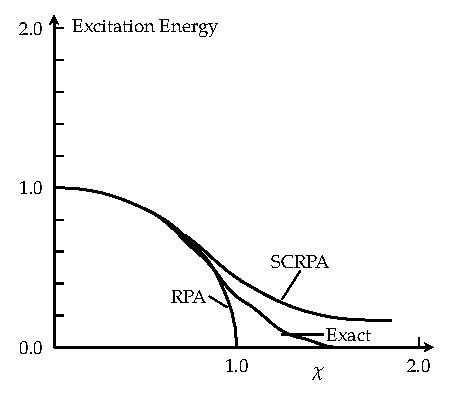
\includegraphics[width=0.7\textwidth]{pictures/9_2}
\par\end{centering}
\caption{\label{fig:9.2}自洽 RPA（SCRPA）与常规 RPA 以及 Lipkin 模型的精确解随相互作用强度参数 $\chi$
的变化对比（引自 \cite{SE73}）。}
\end{figure}

图 9.2 展示了该方法在 Lipkin 模型中的求解结果。我们可以极其清晰地看到，常规 RPA 在相变点区域的崩溃灾难（如 8.8.2
节所述）是如何通过计及玻色展开中的高阶项而得以完全避免的。当粒子数极其巨大时，SCRPA 与 RPA 逐渐趋于重合，这表明在宏观极限下可以出现严格的尖锐相变，而在有限核体系中，量子涨落总会在一定程度上将相变边界平滑地抹开（参见第
11 章）。

\subsubsection{限制在少数集体玻色子情形\label{subsubsec:9.2.3.2_=009650=005236=005728=005C11=006570=0096C6=004F53=0073BB=008272=005B50=0060C5=005F62}}

在某些具体核体系中，存在着充分的物理理由将动力学自由度限制在少数几个关键集体玻色子（如四极振动与配对振动）之内。此时，无限级数展开（式
9.43）通常不再能精确满足对易代数。追随 Sørensen 的构想 \cite{So67}，我们仍然可以采用截断至固定玻色子算符数目的拟设（式
9.40），并将展开参数 $x^{(1)},x^{(3)},\ldots,x^{(2n+1)}$ 以及 $y^{(0)},y^{(2)},\ldots,y^{(2n)}$
视为待定未知数。将该拟设直接代入对易代数中，通过计算对易子并令同类算符的展开系数彼此相等，我们便可获得一组关于系数 $x^{(i)}$
与 $y^{(i)}$ 的代数方程组（通常为非线性方程组）。例如在仅包含单一玻色子的情况下：
\begin{align}
1-y^{(0)} & =|x^{(1)}|^{2},\nonumber \\
-y^{(2)} & =2\left(|x^{(3)}|^{2}+x^{*}_{1}x_{3}+x^{*}_{3}x_{1}\right),\label{eq:9.52}\\
 & \;\;\vdots\nonumber 
\end{align}
求解这些方程组是完全可行的，Sørensen 将其计算推进至第四阶 \cite{So67,So68a,So68b,So69,So70,So71,So73}，而
Kishimoto 和 Tamura 则进一步在 Hamiltonian 中推进至第六阶 \cite{KT72,KT76}（另见
\cite{SP77b}）。然而，在方程组中常数参数 $y^{(0)}$ 始终是一个自由选取的开参数。改变该参数相当于在玻色子空间内部执行一次么正变换
\cite{So68b}。它对展开的收敛特性具有显著影响，并在文献中被以不同方式加以利用。

这种类型的玻色展开在本质上不再属于严格的微扰展开，因为当在拟设中计入更高阶项时，原有特定阶数上的系数数值也会随之发生修正。在此意义上，它能够更好地自适应于所考察的特定集体玻色子。至于
Hamiltonian 不应将集体子空间与 Hilbert 空间其余部分强烈耦合的动力学判据，在此类考量中依然必须得到严格遵守。

\subsection{Marumori 玻色展开\label{subsec:9.2.4_Marumori=0073BB=008272=005C55=005F00}}

Marumori 等人 \cite{MYT64a,MYT64b} 提出了一种从费米子空间到玻色子物理子空间态矢量的一一对应映射方法。该步骤最初是针对非集体玻色子给出的，我们将在
\ref{subsec:9.2.6_=006570=005B66=0080CC=00666F} 中对相关数学细节进行简要评述。由于在非集体情形下收敛性极差，Holzwarth
等人 \cite{LH75} 在实际计算中发展了一种采用少数集体玻色子的修正方案。该方法也已被成功应用于严格可解模型中 \cite{PKD68,KI69}。

从式 \ref{eq:9.24} 形式的集体费米子对算符 $b^{\dagger}_{\mu}$ 出发，我们引入归一化的 $2n$-费米子态：
\begin{equation}
|n\rangle=\mathscr{N}_{F}(n)|\mu_{1}\cdots\mu_{n}\rangle=\mathscr{N}_{F}(n)b^{\dagger}_{\mu_{1}}\cdots b^{\dagger}_{\mu_{n}}|0\rangle,\label{eq:9.53}
\end{equation}
其中 $\mathscr{N}_{F}(n)$ 是归一化常数。一般而言，这些态并不是彼此正交的。然而，只要仅计及少数几个集体算符且数目
$n$ 不是过大（即粒子总数不超过相应费米子空间的容纳限度），我们假定它们是线性独立的。其重叠范数矩阵 $N_{nn'}$ 定义为：
\begin{equation}
N_{nn'}=\langle\mu_{1}\cdots\mu_{n}|\mu'_{1}\cdots\mu'_{n'}\rangle.\label{eq:9.54}
\end{equation}
它与式 \ref{eq:9.28a} 中的量 $\Gamma$ 密切相关：
\begin{align}
N_{11}:\quad\langle\mu|\mu'\rangle & =\delta_{\mu\mu'},\nonumber \\
N_{22}:\quad\langle\mu\nu|\mu'\nu'\rangle & =\delta_{\mu\mu'}\delta_{\nu\nu'}+(\mu\leftrightarrow\nu)-\Gamma^{\mu\nu}_{\mu'\nu'},\label{eq:9.55}\\
N_{33}:\quad\langle\mu\nu\rho|\mu'\nu'\rho'\rangle & =\delta_{\mu\mu'}\delta_{\nu\nu'}\delta_{\rho\rho'}-\delta_{\rho\rho'}\Gamma^{\mu\nu}_{\mu'\nu'}-\Gamma^{\mu\nu\rho}_{\mu'\nu'\rho'}+(\text{若干对换项}).\nonumber 
\end{align}
对角矩阵元决定了归一化因子；例如对于双声子态的归一化因子，我们有：
\begin{equation}
\mathscr{N}_{F}(2)=\left(1+\delta_{\mu\nu}-\Gamma^{\mu\nu}_{\mu\nu}\right)^{-1/2}.\label{eq:9.56}
\end{equation}
Marumori 现在引入由归一化正交基底所张成的玻色子空间：
\begin{equation}
|n)=\mathscr{N}_{B}(n)|\mu_{1}\cdots\mu_{n})=\mathscr{N}_{B}(n)B^{\dagger}_{\mu_{1}}\cdots B^{\dagger}_{\mu_{n}}|0).\label{eq:9.57}
\end{equation}
其中 $\mathscr{N}_{B}$ 是形如 $(n_{1}!n_{2}!\cdots)^{-1/2}$ 的平庸组合因子（参见附录
C.19）。算符
\begin{equation}
U=\sum_{nn'}|n)N^{-1/2}_{nn'}\langle n'|\cdot\mathscr{N}^{-1}_{F}(n')\label{eq:9.58}
\end{equation}
将费米子空间映射到该玻色子空间中。在许多实际应用中（参见 \ref{subsec:9.2.8_=005E94=007528}），重叠矩阵
$N$ 是对角化的，否则算符 $N^{-1/2}$ 的作用即代表正交化过程。因此我们局限于此情形，并将物理算符变换到玻色子空间中：
\begin{equation}
H_{B}=UHU^{\dagger}=\sum_{nn'}\langle n|H|n'\rangle|n)(n'|.\label{eq:9.59}
\end{equation}
玻色子空间中的算符 $|n)(n'|$ 可以通过作用在玻色子真空上的投影算符来表达\footnote{双冒号 ${:}\cdots{:}$ 表示算符的正规乘积。式 \ref{eq:9.60} 的关系在单玻色子情形下极易直接证明：$B|0)(0|=B(1-B^{\dagger}B+\frac{1}{2}B^{\dagger}B^{\dagger}BB-\cdots)=B-B+B^{\dagger}BB-B^{\dagger}BB+\cdots=0$。}：
\begin{equation}
|0)(0|={:}\exp\left(-\sum_{\mu}B^{\dagger}_{\mu}B_{\mu}\right){:}=1_{B}-\sum_{\mu}B^{\dagger}_{\mu}B_{\mu}+\frac{1}{2!}\sum_{\mu\nu}B^{\dagger}_{\mu}B^{\dagger}_{\nu}B_{\mu}B_{\nu}-\cdots\label{eq:9.60}
\end{equation}
用显然的简记符号可以写为：
\begin{equation}
|n)(n'|=\mathscr{N}_{B}(n)\mathscr{N}_{B}(n')(B^{\dagger})^{n}\left(1-\cdots B^{\dagger}B+\cdots B^{\dagger}B^{\dagger}BB-\cdots\right)(B)^{n'}.\label{eq:9.61}
\end{equation}
如果 $|n\rangle$ 仅代表少数几个集体激发态，则 Hamiltonian（式 9.59）仅对应于多体 Hamiltonian
的集体部分，其本征态仅在全 Hamiltonian 不将集体子空间与 Hilbert 空间其余部分强烈耦合时才具有确定的物理意义。因此，合适玻色子的选择高度依赖于敏锐的物理直觉。

在式 \ref{eq:9.59} 中，集体 Hamiltonian 被表示为玻色子算符的正规序幂级数。它包含了多体 Hamiltonian
在集体子空间中的费米子矩阵元以及玻色子真空投影算符的展开式（式 9.60）。正如我们将看到的，在求和式 \ref{eq:9.59}
中通常仅需计及较小的 $n$ 和 $n'$ 值即可给出优良近似：$n+n'\le n_{\text{max}}$。因此，在实际应用中我们仅需要低阶的费米子矩阵元
$\langle n|H|n'\rangle$。这正是玻色子理论的核心实用优势。它们是在集体费米子对基底中、利用 Hamiltonian
的表象式 \ref{eq:9.32} 计算出来的。例如考虑矩阵元 $\langle n+2|H|n\rangle$，我们有：
\begin{equation}
\langle\mu_{1}\cdots\mu_{n+2}|H|\nu_{1}\cdots\nu_{n}\rangle=\sum_{\rho\sigma}V^{40}_{\rho\sigma}\langle\mu_{1}\cdots\mu_{n+2}|\rho\sigma\nu_{1}\cdots\nu_{n}\rangle.\label{eq:9.62}
\end{equation}
在假定 Hamiltonian 不散射出集体空间的条件下，对 $\rho$ 和 $\sigma$ 的求和被严格限制在少数几个集体指标之内，从而将问题归结为计算范数矩阵元（式
9.54）。这在实际计算中是一项相当繁复的工作，因为它们通过式 \ref{eq:9.28a} 中的 $\Gamma$ 量全面计入了
Pauli 原理的修正。

在此步骤中，人们通常采用一个额外的实用近似：若右侧对 $\rho$ 的求和仅遍历集体子空间中的态，则对易关系 \ref{eq:9.27c}
已经在集体空间内部得到了充分满足。这意味着双重对易子
\begin{equation}
\left[b_{\mu},[b_{\mu'},b^{\dagger}_{\nu'}]\right]=-\sum_{\rho}\Gamma^{\mu'\mu}_{\nu'\rho}b_{\rho}\label{eq:9.63}
\end{equation}
不会散射出集体空间之外；这一近似我们在 Belyaev-Zelevinski 理论中已经使用过。

利用式 \ref{eq:9.27b} 与 \ref{eq:9.27c}，我们随后可以导出范数矩阵元的递推关系 \cite{HJJ76,IST77,SP78}：
\begin{align}
\langle\mu_{1}\cdots\mu_{n}|\nu_{1}\cdots\nu_{n}\rangle & =\delta_{\mu_{1}\nu_{1}}\langle\mu_{2}\cdots\mu_{n}|\nu_{2}\cdots\nu_{n}\rangle\nonumber \\
 & \quad+\sum(\mu_{1}\text{ 与所有 }\mu_{2}\cdots\mu_{n}\text{ 对换})\nonumber \\
 & \quad-\sum_{\lambda}\Gamma^{\mu_{1}\mu_{2}}_{\nu_{1}\lambda}\langle\lambda\mu_{3}\cdots\mu_{n}|\nu_{2}\cdots\nu_{n}\rangle\nonumber \\
 & \quad-\sum\left[\mu_{1}\mu_{2}\text{ 与 }(\mu_{1}\cdots\mu_{n})\text{ 中的所有指标对对换}\right].\label{eq:9.64}
\end{align}
从双声子范数（式 9.55）出发，我们因而能够用 $\Gamma^{(2)}$ 表达所有的高阶范数矩阵元。Holzwarth 等人
\cite{HJJ76} 在实际过渡核中检验了该近似的可靠性，发现它与严格的范数矩阵元极其吻合。

我们将在 \ref{subsec:9.2.6_=006570=005B66=0080CC=00666F} 中看到，量 $\langle\mu_{1}\cdots\mu_{n}|\nu_{1}\cdots\nu_{n}\rangle$
正比于投影算符 $\hat{P}$ 在物理子空间中的矩阵元（参见式 9.99）。它们确切地反映了集体双准粒子算符 $b^{\dagger}_{\mu}$
并非真正玻色子这一事实。由这些算符张成的费米子空间是有限维的，而由相应玻色子算符张成的玻色子空间则是无限维的。因此，我们发现费米子范数与玻色子范数的商：
\begin{equation}
\nu(n)=\frac{\langle\mu_{1}\cdots\mu_{n}|\mu_{1}\cdots\mu_{n}\rangle}{(\mu_{1}\cdots\mu_{n}|\mu_{1}\cdots\mu_{n})}\label{eq:9.65}
\end{equation}
对于较大的 $n$ 值迅速跌落至极小。这意味着有效的费米子空间由于 Pauli 原理的压低而被急剧截断。特别地，我们发现耦合不同玻色子数状态的
Hamiltonian 矩阵元 $\langle n+2|H|n\rangle$ 随着 $n$ 的增大而迅速衰减。结果，我们完全可以将式
\ref{eq:9.59} 中的求和截断在很低的 $n$ 和 $n'$ 上。在很多实际问题中 \cite{HJJ76,SP77c}，将
Hamiltonian 的 Marumori 展开保留至四阶或六阶就已经是一种极高精度的优良近似。

总结上述结果，集体 Marumori 展开的有效性建立在两项先决条件之上：
\begin{enumerate}
\item \textbf{运动学条件}（纯粹与集体算符 $b^{\dagger}_{\mu}$ 及 $\Gamma$ 有关）：费米子范数矩阵元必须随着
$n$ 的增加而剧烈下降，从而使高阶项被 Pauli 原理有效截断；
\item \textbf{动力学条件}（与多体 Hamiltonian $H$ 的微观性质有关）：所选取的矢量 $|\mu_{1}\cdots\mu_{n}\rangle$
所张成的集体子空间必须与体系的真实本征子空间高度吻合，即 $H$ 与 Hilbert 空间其余部分的耦合必须极其微弱。
\end{enumerate}
第一项条件表面上似乎与微扰玻色展开中要求高度集体玻色子与微小 $\Gamma$ 值的条件（参见 \ref{subsubsec:9.2.3.1_=005FAE=006270=0073BB=008272=005C55=005F00}）相矛盾。对于微小的
$\Gamma$ 值，有效的费米子空间实际上相当庞大。事实上，第一项条件对于少数纯双准粒子算符而言满足得最好，因为此时有效费米子空间极小。然而在这种极端情况下，第二项动力学条件却几乎无法满足。只有对于真正的集体玻色子，相应的费米子空间才足够丰富，从而允许我们找到体系精确本征态能够被充分逼近的物理情形。事实证明，在这些情况下
Pauli 原理的压低效应依然足够强大，足以保证级数展开的迅速收敛 \cite{HJJ76}。

作为具体示范，我们再次考察 \ref{sec:5.4_Lipkin=006A21=00578B} 中的 Lipkin 模型（详细讨论参见
\cite{PKD68}）。根据式 \ref{eq:9.37} 与 \ref{eq:9.64}，我们得到范数的递推关系：
\begin{equation}
\langle(b)^{n}(b^{\dagger})^{n}\rangle=\langle(b)^{n-1}(b^{\dagger})^{n-1}\rangle\left[n-\frac{n}{2}(n-1)\frac{2}{\Omega}\right],\label{eq:9.66}
\end{equation}
该式在 Lipkin 模型中是严格成立的。对于归一化因子，它给出：
\begin{equation}
\mathscr{N}_{F}(n)=\sqrt{\frac{(\Omega-n)!}{\Omega!n!}\Omega^{n}},\qquad\mathscr{N}_{B}=\frac{1}{\sqrt{n!}}.\label{eq:9.67}
\end{equation}
根据式 \ref{eq:9.59}，保留至四玻色子项的 Hamiltonian（式 9.38）具有如下形式：
\begin{align}
H_{B}=-\frac{\epsilon}{2}\Omega+\epsilon B^{\dagger}B & -V\frac{\Omega}{2}\left[\sqrt{1-\frac{1}{\Omega}}B^{\dagger}B^{\dagger}\right.\nonumber \\
 & \quad\left.-\left(\sqrt{1-\frac{1}{\Omega}}-\sqrt{\left(1-\frac{1}{\Omega}\right)\left(1-\frac{2}{\Omega}\right)}\right)B^{\dagger}B^{\dagger}B^{\dagger}B+\text{h.c.}\right].\label{eq:9.68}
\end{align}
我们看到，Marumori 表象并不对应于 $1/\Omega$ 的渐近展开。每一个展开系数都内含了 $1/\Omega$ 的所有阶贡献。若将这些平方根按
$1/\Omega$ 展开到某一固定阶数，就能完全恢复出与 Belyaev-Zelevinski 展开等价的各项（式 9.47）。反之，通过对
Belyaev-Zelevinski 展开的所有阶项进行正规序重排，并对属于固定玻色子数目的算符系数进行全面求和，也能够精确导出 Marumori
Hamiltonian，因为两种展开在无穷阶意义下是严格等价的（参见 \ref{subsec:9.2.6_=006570=005B66=0080CC=00666F}）。Marumori
展开的不可替代的优势在于：它在每一个有限阶数 $n$ 上都严格计入了 Pauli 原理。

事实上，将 Marumori 算符在至多包含 $N_{\text{max}}$ 个玻色子的截断玻色子空间中对角化，精确等价于将费米子
Hamiltonian 在由费米子态 $|n\rangle$（$n\le N_{\text{max}}$）所张成的子空间中对角化。在后一种做法中，我们必须显式计算费米子矩阵元
$\langle n|H|n'\rangle$。从式 \ref{eq:9.59} 可以看出，这些量正是 Marumori 算符在玻色子空间中的矩阵元
$(n|H_{B}|n')$。转录到玻色子图象的优越性在于：在上述物理条件下，对 $n$ 的求和可以安全地限制在一个很小的上限
$n_{\text{max}}$ 上。这意味着高阶矩阵元 $(n|H_{B}|n')$ 可以完全用仅包含低阶费米子矩阵元的求和式表达出来。

若我们计入所有的费米子对 $b^{\dagger}_{\mu}$（包括所有的非集体对），Marumori 方法就精确对应于在 $2N_{\text{max}}$-准粒子空间中的壳模型组态相互作用计算。因此在最低阶近似下，我们得到的不是
RPA，而是 TDA 近似。

\subsection{Dyson 玻色展开\label{subsec:9.2.5_Dyson=0073BB=008272=005C55=005F00}}

迄今为止所讨论的玻色子表象都是无穷阶级数展开，它们仅在某些特定物理条件（例如底层费米子对具有极高集体性）下才具有良好的收敛性。在某些情况下——尤其是紧邻闭壳层的核体系中——我们必须显式计及其他集体性较弱的双费米子对及其与集体子空间的相互混合。在这些情形下，我们必须允许引入多种具有不同集体性程度的玻色子。尽管如此，人们依然希望至少对于核体系的低激发态，展开能够关于不同类型玻色子的数目
$m$ 迅速收敛。

这代表了一种截然不同的收敛类型（即图 9.3 中的垂直方向）。借助 Dyson 的玻色子表象，人们能够系统地研究这一问题，因为该方法最终给出一个严格有限阶截断的玻色子
Hamiltonian。图 9.3 同时也标明了迄今为止文献中所探讨的几类典型物理情形。在软核的过渡区中，人们检验了包含少数几个集体玻色子的水平方向收敛性
\cite{HJJ76}；而在幻核 $^{208}\text{Pb}$ 的邻域中，人们则检验了针对许多不同类型玻色子（但每次仅激发少数几个声子）的垂直方向收敛性
\cite{IRS80}。

一般而言，体系很可能在某些状态下既需要激发许多不同类型的玻色子，又需要激发同一类型的多个声子；这一极端复杂的区域在图 9.3 中用问号标出，至今仍是理论处理上的前沿挑战。

\begin{figure}[H]
\begin{centering}
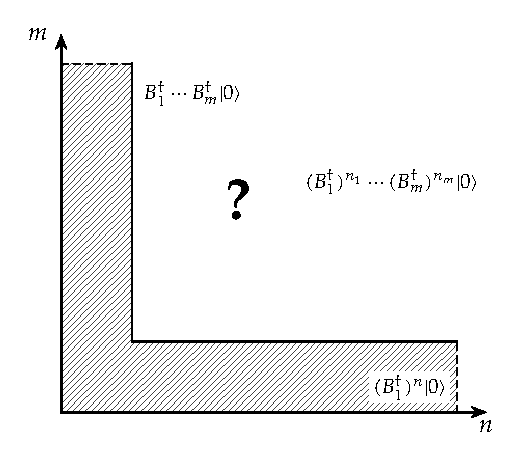
\includegraphics[width=0.7\textwidth]{pictures/9_3}
\par\end{centering}
\caption{\label{fig:9.3}玻色展开中所面临的两种收敛类型的示意图。$m$ 给出了不同玻色子类型的数目 $B^{\dagger}_{1}\cdots B^{\dagger}_{m}$，而
$n$ 给出了同一类型玻色子的激发数目 $(B^{\dagger}_{1})^{n}$。}
\end{figure}

Dyson 表象建立在如下数学事实之上：通过引入非厄米映射，对易子代数 \ref{eq:9.27a} 可以通过如下严格有限的变换精确满足\footnote{该表象的早期版本形式，另见 \cite{Am67}。}
\cite{RS77a}：
\begin{align}
b^{\dagger}_{\mu}\to\tilde{B}^{\dagger}_{\mu} & =B^{\dagger}_{\mu}-\frac{1}{2}\sum_{\nu\rho\sigma}\Gamma^{\nu\rho}_{\mu\sigma}B^{\dagger}_{\nu}B^{\dagger}_{\rho}B_{\sigma},\label{eq:9.69a}\\
b_{\mu}\to B_{\mu},\label{eq:9.69b}\\
a_{\mu\nu}\to\sum_{\rho\sigma}\Gamma^{\mu\rho}_{\nu\sigma}B^{\dagger}_{\rho}B_{\sigma}.\label{eq:9.69c}
\end{align}
这是角动量代数的 Dyson 表象（式 9.9）向多体问题的直接推广。通过将费米子真空 $|0\rangle$ 映射为玻色子真空
$|0)$，我们便得到了 Hilbert 空间中态矢量的相应表示。

利用式 \ref{eq:9.32} 与 \ref{eq:9.69a} 的严格有限表达式，我们导出了一个有限截断的玻色子 Hamiltonian，它最高仅包含算符
$B$ 与 $B^{\dagger}$ 的六阶项。算符 $H^{11}$ 与 $H^{22}$ 保持玻色子数守恒。假定展开系数
$C^{\mu}_{kl}$ 由 TDA 方程（式 8.10）所确定，经过直接推导可得：
\begin{equation}
V^{22}_{\mu\nu}=\delta_{\mu\nu}\Omega_{\mu}-\sum_{k}\Gamma^{\mu k}_{\nu k}E_{k},\label{eq:9.70}
\end{equation}
以及
\begin{equation}
H^{11}+H^{22}=\sum_{\mu}\Omega_{\mu}B^{\dagger}_{\mu}B_{\mu}+\frac{1}{4}\sum_{\mu\nu\rho\sigma}W_{\mu\nu\rho\sigma}B^{\dagger}_{\mu}B^{\dagger}_{\nu}B_{\rho}B_{\sigma},\label{eq:9.71}
\end{equation}
其中的相互作用矩阵元为：
\begin{equation}
W_{\mu\nu\rho\sigma}=\sum_{klpq}C^{\mu*}_{kl}C^{\nu*}_{pq}C^{\rho}_{kp}C^{\sigma}_{lq}(E_{k}+E_{l}+E_{p}+E_{q}-\Omega_{\rho}-\Omega_{\sigma}).\label{eq:9.72}
\end{equation}
Hamiltonian 中的其余项破坏玻色子数守恒，其显式形式可在文献 \cite{RS77a} 中找到。

Dyson 表象的一个显著缺点在于它破坏了 Hermite 性，这从式 \ref{eq:9.71} 中的有效相互作用 $W$ 便可清晰看出。态矢与左矢在玻色子空间中的对应像为：
\[
|\mu_{1}\cdots\mu_{n}\rangle\to\tilde{B}^{\dagger}_{\mu_{1}}\cdots\tilde{B}^{\dagger}_{\mu_{n}}|0),\qquad\langle\mu_{1}\cdots\mu_{n}|\to(0|B_{\mu_{n}}\cdots B_{\mu_{1}},
\]
它们彼此之间不再构成正交基底。与式 \ref{eq:9.54} 类似，重叠范数矩阵 $N$ 为：
\begin{equation}
N(\mu_{1}\cdots\mu_{n},\mu'_{1}\cdots\mu'_{n})=(0|B_{\mu_{1}}\cdots B_{\mu_{n}}\tilde{B}^{\dagger}_{\mu'_{1}}\cdots\tilde{B}^{\dagger}_{\mu'_{n}}|0).\label{eq:9.73}
\end{equation}
由于现代科学计算中存在针对大型非 Hermite 矩阵的高效对角化算法，因此这在实用中并不是致命障碍 \cite{RS74b,SWR76,Sch76}。我们将在
\ref{subsec:9.2.6_=006570=005B66=0080CC=00666F} 与 \ref{subsec:9.3.6_=004E2D=007B49=008026=005408=004E0EDyson=0073BB=008272=005C55=005F00}
中探讨其更深层次的数学细节。

如果能够合理忽略具有不同玻色子数目的子空间之间的相互耦合，该方法就会变得异常简捷。在那些情形下，有效 Hamiltonian 仅由
$H^{11}+H^{22}$ 所完全表征，并能够完全用 TDA 振幅 $C^{\mu}_{kl}$、TDA 本征激发能 $\Omega_{\mu}$
以及单准粒子能量 $E_{k}$ 显式解析表达。

\subsection{数学背景\label{subsec:9.2.6_=006570=005B66=0080CC=00666F}}

在本小节中，我们将系统探讨迄今为止所处理的各种玻色子表象的深层数学性质，从而厘清不同理论方法之间的内在数学联系。对于不深究这些高度专门化数学推导的读者，可以略过本节。受篇幅所限，我们无法在此给出所有漫长繁复的推导细节，相关步骤请读者参阅原始文献。

为了透彻理解玻色子表象的数学架构，使用“非集体”玻色子 $B_{kl}=-B_{lk}$ 是极其方便的。它们的指标精确对应于费米子对（式
9.22），并服从标准玻色子对易关系：
\begin{equation}
[B_{kl},B_{k'l'}]=0,\qquad[B_{kl},B^{\dagger}_{k'l'}]=\delta_{kk'}\delta_{ll'}-(k\leftrightarrow l).\label{eq:9.74}
\end{equation}
从多费米子空间的一组完备正交基底
\begin{equation}
|n\rangle=|k_{1}l_{1}\cdots k_{n}l_{n}\rangle=\alpha^{\dagger}_{k_{1}}\alpha^{\dagger}_{l_{1}}\cdots\alpha^{\dagger}_{k_{n}}\alpha^{\dagger}_{l_{n}}|0\rangle\label{eq:9.75}
\end{equation}
出发，我们可以在玻色子空间中定义相应的正交态矢集合 \cite{MYT64a}：
\begin{equation}
|n)=\frac{1}{\sqrt{(2n-1)!!}}\sum_{P}(-)^{P}B^{\dagger}_{k_{1}l_{1}}\cdots B^{\dagger}_{k_{n}l_{n}}|0),\label{eq:9.76}
\end{equation}
其中 $P$ 遍历指标 $k_{1}\ldots l_{n}$ 的所有能够给出新玻色子组合 $B^{\dagger}_{k_{1}l_{1}}\cdots B^{\dagger}_{k_{n}l_{n}}$
的置换（即 $B^{\dagger}_{12}B^{\dagger}_{34}$ 与 $B^{\dagger}_{34}B^{\dagger}_{21}$
仅被计入一次）；总项数为 $(2n)!/(n!2^{n})=(2n-1)!!$ 项。

式 \ref{eq:9.76} 中的态矢 $|n)$ 张成了玻色子空间的一个线性子空间，即所谓的\textbf{物理子空间}。正如我们将证明的，在这一子空间与原费米子空间之间存在着严格的一一对应关系。玻色子空间的其余部分则包含了形如
$B^{\dagger}_{k_{1}l_{1}}\cdots B^{\dagger}_{k_{n}l_{n}}|0)$ 但在指标
$k_{1}\ldots l_{n}$ 上未完全反对称化的状态，它们实质上破坏了 Pauli 原理。含有此类成分的状态会对物理算符的期望值产生虚假的赝态贡献。

Janssen 等人 \cite{JDF71} 证明，式 \ref{eq:9.76} 中的基态矢还可以写为如下优美形式：
\begin{align}
|n) & =\frac{1}{\sqrt{(2n-1)!!}}\langle0|\exp\left\{ \frac{1}{2}\sum_{kl}B^{\dagger}_{kl}\alpha_{l}\alpha_{k}\right\} \alpha^{\dagger}_{k_{1}}\alpha^{\dagger}_{l_{1}}\cdots\alpha^{\dagger}_{k_{n}}\alpha^{\dagger}_{l_{n}}|0\rangle|0)\label{eq:9.77}\\
 & =\frac{1}{\sqrt{(2n-1)!!}}\tilde{B}^{\dagger}_{k_{1}l_{1}}\cdots\tilde{B}^{\dagger}_{k_{n}l_{n}}|0),\label{eq:9.78}
\end{align}
其中引入了非集体 Dyson 算符（式 9.69a）：
\begin{equation}
\tilde{B}^{\dagger}_{kl}=B^{\dagger}_{kl}-\sum_{pq}B^{\dagger}_{kp}B^{\dagger}_{lq}B_{pq}.\label{eq:9.79}
\end{equation}
作为示例，双玻色子基态显式为：
\begin{equation}
|2)=\frac{1}{\sqrt{3}}\tilde{B}^{\dagger}_{k_{1}l_{1}}\tilde{B}^{\dagger}_{k_{2}l_{2}}|0)=\frac{1}{\sqrt{3}}\left(B^{\dagger}_{k_{1}l_{1}}B^{\dagger}_{k_{2}l_{2}}-B^{\dagger}_{k_{1}k_{2}}B^{\dagger}_{l_{1}l_{2}}+B^{\dagger}_{l_{1}k_{2}}B^{\dagger}_{k_{1}l_{2}}\right)|0).\label{eq:9.80}
\end{equation}
投向物理子空间的投影算符 $\hat{P}$ 具有如下显式表达：
\begin{equation}
\hat{P}=\sum_{n}|n)(n|=\sum^{\infty}_{n=0}\frac{1}{(2n)!(2n-1)!!}\sum_{\substack{k_{1}\cdots k_{n}\\
l_{1}\cdots l_{n}
}
}\tilde{B}^{\dagger}_{k_{1}l_{1}}\cdots\tilde{B}^{\dagger}_{k_{n}l_{n}}|0)(0|\tilde{B}_{k_{n}l_{n}}\cdots\tilde{B}_{k_{1}l_{1}}.\label{eq:9.81}
\end{equation}
经过直接应用关系式
\begin{align}
\sum_{\substack{k_{1}\cdots k_{n}\\
l_{1}\cdots l_{n}
}
}\tilde{B}^{\dagger}_{k_{1}l_{1}}\cdots\tilde{B}^{\dagger}_{k_{n}l_{n}}|0)(0|\tilde{B}_{k_{n}l_{n}}\cdots\tilde{B}_{k_{1}l_{1}} & =(2n-1)!!\sum_{\substack{k_{1}\cdots k_{n}\\
l_{1}\cdots l_{n}
}
}\tilde{B}^{\dagger}_{k_{1}l_{1}}\cdots\tilde{B}^{\dagger}_{k_{n}l_{n}}|0)(0|B_{k_{n}l_{n}}\cdots B_{k_{1}l_{1}}\label{eq:9.82}
\end{align}
与
\begin{align}
(0|\tilde{B}_{p_{n}q_{n}}\cdots\tilde{B}_{p_{1}q_{1}}\tilde{B}^{\dagger}_{k_{1}l_{1}}\cdots\tilde{B}^{\dagger}_{k_{n}l_{n}}|0) & =(2n-1)!!(0|B_{p_{n}q_{n}}\cdots B_{p_{1}q_{1}}\tilde{B}^{\dagger}_{k_{1}l_{1}}\cdots\tilde{B}^{\dagger}_{k_{n}l_{n}}|0),\label{eq:9.83}
\end{align}
并定义算符
\begin{equation}
(B^{\dagger}B)_{kl}=\sum_{q}B^{\dagger}_{ql}B_{qk},\qquad\hat{N}=\frac{1}{2}\sum_{kl}B^{\dagger}_{kl}B_{kl},\label{eq:9.84}
\end{equation}
我们可以证明投影算符具有下列核心代数性质：
\begin{align}
[\hat{P},\tilde{B}^{\dagger}_{kl}] & =0,\qquad\hat{P}B_{kl}\hat{P}=B_{kl}\hat{P},\qquad[\hat{P},(B^{\dagger}B)_{kl}]=0,\label{eq:9.85}\\
\tilde{B}^{\dagger}_{kl}\hat{P} & =\hat{P}B^{\dagger}_{kl}(1+2\hat{N}),\qquad2\hat{P}B^{\dagger}_{kl}\hat{N}=-\hat{P}\left(B^{\dagger}\cdot(B^{\dagger}B)\right)_{kl}.\label{eq:9.86}
\end{align}
将费米子空间映射到玻色子物理子空间的方法有多种可能。Usui \cite{Us60} 引入了变换算符：
\begin{equation}
\bar{U}=\langle0|\exp\left\{ \frac{1}{2}\sum_{kl}B^{\dagger}_{kl}\alpha_{l}\alpha_{k}\right\} |0).\label{eq:9.87}
\end{equation}
在费米子空间中插入完备系（式 9.75）并利用式 \ref{eq:9.77}，该算符可写作：
\begin{equation}
\bar{U}=\sum_{n}\sqrt{(2n-1)!!}\,|n)(n|.\label{eq:9.88}
\end{equation}
它显然不是么正算符。因此，我们必须定义其共轭映射算符：
\begin{equation}
\tilde{U}=\sum_{n}\frac{1}{\sqrt{(2n-1)!!}}\,|n\rangle(n|=\bar{U}^{\dagger}\left((2\hat{N}-1)!!\right)^{-1},\label{eq:9.89}
\end{equation}
其中 $\hat{N}$ 是玻色子数算符（式 9.84）。若 $1_{F}$ 是费米子空间的单位算符，则有：
\begin{equation}
\tilde{U}\bar{U}=1_{F},\qquad\bar{U}\tilde{U}=\hat{P}.\label{eq:9.90}
\end{equation}
费米子对算符（式 9.22）在这一变换下的映射行为如下：
\begin{align}
b^{\dagger}_{kl} & \to\bar{U}\alpha^{\dagger}_{k}\alpha^{\dagger}_{l}\tilde{U}=\tilde{B}^{\dagger}_{kl}\cdot\hat{P},\nonumber \\
b_{kl} & \to\bar{U}\alpha_{l}\alpha_{k}\tilde{U}=B_{kl}\cdot\hat{P},\label{eq:9.91}\\
a_{kl} & \to\bar{U}\alpha^{\dagger}_{l}\alpha_{k}\tilde{U}=(B^{\dagger}B)_{kl}\cdot\hat{P}.\nonumber 
\end{align}
该变换显然精确对应于 \ref{subsec:9.2.5_Dyson=0073BB=008272=005C55=005F00} 中所讨论的
Dyson 表象。相应的玻色子有效 Hamiltonian 具有如下形式：
\begin{equation}
\bar{U}H\tilde{U}=H_{B}\cdot\hat{P},\label{eq:9.92}
\end{equation}
其中
\begin{align}
H_{B} & =\sum_{k}E_{k}(B^{\dagger}B)_{kk}+\sum_{klpq}\left(H^{40}_{klpq}\tilde{B}^{\dagger}_{kl}\tilde{B}^{\dagger}_{pq}+H^{40*}_{klpq}B_{kl}B_{pq}\right)\nonumber \\
 & \quad+\sum_{klpq}\left(H^{31}_{klpq}\tilde{B}^{\dagger}_{kl}(B^{\dagger}B)_{qp}+H^{31*}_{klpq}(B^{\dagger}B)_{pq}B_{kl}\right)\nonumber \\
 & \quad+\frac{1}{4}\sum_{klpq}H^{22}_{klpq}\tilde{B}^{\dagger}_{kl}B_{pq}.\label{eq:9.93}
\end{align}
只要我们将波函数严格局限在物理子空间内，就可以安全地省去投影算符 $\hat{P}$，并直接求解 Schrödinger 方程：
\begin{equation}
H_{B}|\Psi)=E|\Psi).\label{eq:9.94}
\end{equation}
然而我们必须警惕：方程中不可避免地存在着源于破坏 Pauli 原理的非物理赝解（spurious solutions）$|\Psi_{s})$。由于
$\hat{P}$ 与 $H_{B}$ 并不对易，这些赝态解可能具有物理子空间的分量，即 $\hat{P}|\Psi_{s})\ne0$。为了识别它们，必须检验判据
$(1-\hat{P})|\Psi_{s})\ne0$。在通过限制集体玻色子数目来对本征值问题进行近似求解时，赝解可能会与真实物理态相互混杂。为此，将
Hamiltonian 进行如下分解通常极具启发意义：
\begin{equation}
H_{B}=H^{0}_{B}+V_{B},\label{eq:9.95}
\end{equation}
其中 $H^{0}_{B}=\sum_{k}E_{k}(B^{\dagger}B)_{kk}$。由式 \ref{eq:9.85}
可知，$H^{0}_{B}$ 与 $\hat{P}$ 严格对易。因此，方程 \ref{eq:9.94} 的物理真解也必定满足方程：
\begin{equation}
\left(H^{0}_{B}+\hat{P}V_{B}\right)|\Psi)=E|\Psi).\label{eq:9.96}
\end{equation}
将任意本征解分解为物理部分与赝态部分：$|\Psi)=\hat{P}|\Psi)+(1-\hat{P})|\Psi)$，我们看到其赝态部分必然是
$H^{0}_{B}$ 对应于本征值 $E$ 的本征矢量：
\begin{equation}
H^{0}_{B}(1-\hat{P})|\Psi)=E(1-\hat{P})|\Psi),\label{eq:9.97}
\end{equation}
即式 \ref{eq:9.96} 的所有非物理赝解均精确拥有 $H^{0}_{B}$ 的本征值：
\begin{equation}
E_{k_{1}}+E_{l_{1}}+E_{k_{2}}+E_{l_{2}}+\cdots\label{eq:9.98}
\end{equation}
由于 $H^{0}_{B}$ 最低阶的赝本征函数是形如 $B^{\dagger}_{12}B^{\dagger}_{12}|0)$
的双玻色子态，因此式 \ref{eq:9.96} 的最低赝解位于自由四准粒子能量处。这通常远高于所感兴趣的低激发集体谱区，因而式
\ref{eq:9.96} 的近似求解不会导致物理态与非物理态之间的严重混杂。

在实际应用中，从集体玻色子出发是极为明智的。Hamiltonian $H_{B}$ 的集体形式已经在 \ref{subsec:9.2.5_Dyson=0073BB=008272=005C55=005F00}
中推导出来。为了应用式 \ref{eq:9.96}，我们仅需要投影算符 $\hat{P}$ 的矩阵元。由式 \ref{eq:9.81}
可知，它们直接由范数矩阵元（式 9.54 或 9.73）给出：
\begin{align}
(\mu_{1}\cdots\mu_{n}|\hat{P}|\mu'_{1}\cdots\mu'_{n}) & =(0|B_{\mu_{1}}\cdots B_{\mu_{n}}\hat{P}B^{\dagger}_{\mu'_{1}}\cdots B^{\dagger}_{\mu'_{n}}|0)\nonumber \\
 & =\frac{1}{(2n-1)!!}\langle\mu_{1}\cdots\mu_{n}|\mu'_{1}\cdots\mu'_{n}\rangle.\label{eq:9.99}
\end{align}
一旦获得了式 \ref{eq:9.94} 或 \ref{eq:9.96} 的物理本征解，我们便可以通过将跃迁算符 $Q$ 变换到玻色子空间来计算其跃迁矩阵元：
\begin{equation}
\bar{U}Q\tilde{U}=Q_{B}\cdot\hat{P},\label{eq:9.100}
\end{equation}
并进而得出：
\begin{align}
\langle\Psi|Q|\Psi\rangle & =\langle\Psi|\tilde{U}\bar{U}Q\tilde{U}\bar{U}|\Psi\rangle=(\Psi|Q_{B}\hat{P}|\Psi)\nonumber \\
 & =(\Psi|Q_{B}|\Psi).\label{eq:9.101}
\end{align}
这雄辩地表明：只要确信波函数 $|\Psi)$ 不含赝态成分，我们就能完全在玻色子空间内部完成所有感兴趣物理量的计算，而根本无需重新变换回费米子空间。在实用中，这可以通过将范数矩阵（式
9.99）对角化并严格限制在具有非零本征值的子空间中来实现。

Marumori 通过引入严格的么正映射来规避非 Hermite 算符：
\begin{equation}
U=\sum_{n}|n)(n|=\left((2\hat{N}-1)!!\right)^{-1/2}\bar{U},\label{eq:9.102}
\end{equation}
并利用式 \ref{eq:9.91} 与 \ref{eq:9.86} 导出：
\begin{align}
b^{\dagger}_{kl} & \to U\alpha^{\dagger}_{k}\alpha^{\dagger}_{l}U^{\dagger}=\tilde{B}^{\dagger}_{kl}(1+2\hat{N})^{-1/2}\hat{P}=\hat{P}\left(B^{\dagger}\sqrt{1-B^{\dagger}B}\right)_{kl}\hat{P},\nonumber \\
b_{kl} & \to U\alpha_{l}\alpha_{k}U^{\dagger}=(1+2\hat{N})^{-1/2}\tilde{B}_{kl}\hat{P}=\hat{P}\left(\sqrt{1-B^{\dagger}B}\cdot B\right)_{kl}\hat{P},\label{eq:9.103}\\
a_{kl} & \to U\alpha^{\dagger}_{l}\alpha_{k}U^{\dagger}=\hat{P}(B^{\dagger}B)_{kl}\hat{P}.\nonumber 
\end{align}
在所有实际应用中，式 \ref{eq:9.102} 中的平方根都必须用 Taylor 级数替代。因此，即使限制在物理子空间内，Marumori
理论最终也会产生无穷级数展开。平方根展开的系数为 $(-)^{n}\binom{1/2}{n}$。因此，式 \ref{eq:9.103}
精确对应于式 \ref{eq:9.43} 中的微扰玻色展开。若推进至无穷阶，它与 Marumori 方法完全等价。后者是在正规序重排后获得的。截断在有限阶时，两种方法之间则存在细微差别
{[}例如在 Lipkin 模型中对比式 9.47 与式 9.68{]}。

我们还清楚地看到：在非集体玻色子情形下，$\sqrt{1-B^{\dagger}B}$ 的形式级数展开并不收敛 \cite{Ok74}。只有通过引入集体玻色子并对相应子空间进行适当的动力学解耦，才能实现
\ref{subsec:9.2.4_Marumori=0073BB=008272=005C55=005F00} 中所论述的快速收敛。

\subsection{基于 pp-玻色子的方法\label{subsec:9.2.7_=0057FA=004E8Epp-=0073BB=008272=005B50=007684=0065B9=006CD5}}

迄今为止，我们所讨论的各种方法都建立在 Fermi 面附近的玻色子基础之上。这些玻色子在良好近似下由粒子-空穴（ph）对或双准粒子对所给出。其自然的直接后果是，在所有这些方法中玻色子数都是不守恒的。相应的有效
Hamiltonian 包含了诸如 $B^{\dagger}B^{\dagger},B^{\dagger}B^{\dagger}B$
等破坏玻色子数守恒的非对角项。

现在我们从一种完全不同的进路出发，即从裸真空 $|-\rangle$（在实际计算中也可以是完全惰性的双闭壳核芯）出发，逐步添加耦合为近似玻色子的双粒子对。单
$j$-壳层中的 Cooper 对\footnote{这与我们用大写字母表示玻色子的惯例有所不同；式 9.104 中的 $S_{+}$ 与式 9.105 中的 $D^{\dagger}_{\mu}$
代表纯粹的集体费米子对。而另一方面，式 9.119 中的算符 $s^{\dagger}$ 和 $d^{\dagger}$ 则是纯粹的理想玻色子。}（式 6.3）便是一个典型例子：
\begin{equation}
S_{+}\propto\sum_{m}C^{00}_{jmj-m}a^{\dagger}_{jm}a^{\dagger}_{j-m},\label{eq:9.104}
\end{equation}
或者四极粒子对：
\begin{equation}
D^{\dagger}_{\mu}\propto\sum_{mm'}C^{2\mu}_{jmjm'}a^{\dagger}_{jm}a^{\dagger}_{jm'}.\label{eq:9.105}
\end{equation}
在 Seniority 方案（\ref{sec:6.2_Seniority=0065B9=006848}）中，我们可以将基态表示为
Cooper 对的乘积（式 6.19）：
\[
|0\rangle\propto(S_{+})^{N/2}|-\rangle,
\]
并通过将一个 $S_{+}$ 算符替换为 $D^{\dagger}_{\mu}$（式 6.27）来构建某些特定的激发态：
\begin{equation}
|2\mu\rangle\propto(S_{+})^{N/2-1}D^{\dagger}_{\mu}|-\rangle.\label{eq:9.106}
\end{equation}
在一般情况下，我们可以从集体双粒子对出发：
\begin{equation}
b^{\dagger}_{\tau}=\frac{1}{2}\sum_{kl}C^{\tau}_{kl}a^{\dagger}_{k}a^{\dagger}_{l},\label{eq:9.107}
\end{equation}
并应用前述各小节所讨论的方法之一来构建玻色子表象。由于体系的真实核子数是严格守恒的，因此在表象中现在仅出现保持玻色子数守恒的项。例如在
Dyson 方法中，我们得到一个有限截断的四阶玻色子 Hamiltonian {[}参见式 \ref{eq:9.71}{]}：
\begin{equation}
H_{B}=\sum_{\tau}\Omega_{\tau}B^{\dagger}_{\tau}B_{\tau}+\frac{1}{4}\sum_{\tau_{1}\tau_{2}\tau_{3}\tau_{4}}W_{\tau_{1}\tau_{2}\tau_{3}\tau_{4}}B^{\dagger}_{\tau_{1}}B^{\dagger}_{\tau_{2}}B_{\tau_{3}}B_{\tau_{4}}.\label{eq:9.108}
\end{equation}
这里的展开系数 $C^{\tau}_{kl}$ 现在是粒子-粒子（pp）TDA 振幅，而 $\Omega_{\tau}$ 则由相应的本征能量给出。在其他表象方法中，我们也会得到类似的
Hamiltonian（可能是无穷阶且保持 Hermite 性，但同样守恒玻色子数）。

该方法的局限性在于：在微观层面上，它仅能应用于具有极少数玻色子的情况，例如紧邻具有完全惰性核芯的幻核。对于远离幻数闭壳层的原子核，我们需要大量的
pp-玻色子，而这些玻色子相应的 $C^{\tau}_{kl}$ 系数原本是在完全惰性核芯的基底上确定的。对于包含大量价核子的体系，这一基底未必依然优良，正如我们在考虑用
$^{16}\text{O}$ 惰性核芯来描述 $^{208}\text{Pb}$ 邻近核这一极端例子时所能轻易想象的那样。因此，对于远离闭壳层的核，若将振幅严格局限在惰性核芯基底上，pp-玻色子描述可能不再有效。然而，我们可以尝试将振幅
$C^{\tau}_{kl}$ 视为可调节参数，并通过例如变分计算来加以确定。

另一方面，由大量玻色子构成的复杂组态通常只能借助群论方法来系统处理。迄今为止，人们主要探讨了唯象模型。在这些模型中，最著名的是 Arima
和 Iachello 的相互作用玻色子模型（$SU(6)$ 模型）\cite{AI75a,AI75b}。它包含两类玻色子：对应于式
\ref{eq:9.104} 中的 Cooper 对的 $s$ 玻色子，以及对应于式 \ref{eq:9.105} 中五个四极对的五个
$d$ 玻色子。该体系的 Hermite 的有效 Hamiltonian 仅包含至多四阶的玻色子数守恒项 {[}参见式 \ref{eq:9.119}{]}：
\[
s^{\dagger}s,\quad d^{\dagger}d,\quad d^{\dagger}d^{\dagger}dd,\quad s^{\dagger}s^{\dagger}ss,\quad d^{\dagger}d^{\dagger}ss,\quad d^{\dagger}d^{\dagger}ds+\text{h.c.}
\]
若忽略描述玻色子间相互作用的四阶项，我们便拥有一个由 $A/2$ 个 $s$ 玻色子的直积所构成的无微扰基态，以及若干 $s$
玻色子被 $d$ 玻色子取代的激发态。最初，该模型纯粹是建立在唯象基础之上引入的。然而对于具有配对加四极相互作用（式 4.141）的单
$j$-壳层，通过将 pp-费米子对映射到合适的玻色子表象上，该模型同样可以从微观角度获得坚实的理论证明 \cite{AOI77}。我们将在下一小节中详细讨论该模型的若干经典应用。

pp-玻色子的另一个典型范例是 \textbf{Schwinger 表象} \cite{BM78}。在单粒子基底中工作，其中 $a^{\dagger}_{m}$
与 $a^{\dagger}_{i}$ 分别在 Fermi 面的上方与下方产生粒子，我们可以引入两类玻色子：对应于产生粒子-空穴型
pp 对 $a^{\dagger}_{m}a^{\dagger}_{i}$（一个在 Fermi 面上，一个在 Fermi 面下）的
$B$ 玻色子 $B^{\dagger}_{mi}$；以及对应于产生全占据型 pp 对 $a^{\dagger}_{i}a^{\dagger}_{j}$（两个粒子均在
Fermi 面以下）的 $A$ 玻色子 $A^{\dagger}_{ij}$。这两类玻色子均为服从标准玻色对易关系的理想玻色子：
\begin{equation}
[B_{mi},B^{\dagger}_{m'i'}]=\delta_{mm'}\delta_{ii'},\qquad[A_{ij},A^{\dagger}_{i'j'}]=\delta_{ii'}\delta_{jj'}-\delta_{ij'}\delta_{ji'}.\label{eq:9.109}
\end{equation}
为了描述偶数体系，我们仅需要单体密度算符 $a^{\dagger}_{k}a_{l}$。它们按如下规则映射：
\begin{align}
a^{\dagger}_{m'}a_{m} & \to(a^{\dagger}_{m'}a_{m})_{B}=\sum_{i}B^{\dagger}_{m'i}B_{mi},\nonumber \\
a^{\dagger}_{i'}a_{i} & \to(a^{\dagger}_{i'}a_{i})_{B}=\sum_{j}A^{\dagger}_{ij}A_{i'j},\label{eq:9.110}\\
a^{\dagger}_{m}a_{i} & \to(a^{\dagger}_{m}a_{i})_{B}=\sum_{j}B^{\dagger}_{mj}A_{ij},\nonumber \\
a^{\dagger}_{i}a_{m} & \to(a^{\dagger}_{i}a_{m})_{B}=(a^{\dagger}_{m}a_{i})^{\dagger}_{B}.\nonumber 
\end{align}
该映射严格保持了密度算符 $a^{\dagger}_{k}a_{l}$ 的对易关系以及 Hermite 性，并且在玻色子空间中给出了严格有限的表达式。从对应于费米子裸真空的玻色子真空
$|-\rangle$ 出发：
\begin{equation}
A_{ij}|-\rangle=B_{mi}|-\rangle=0,\label{eq:9.111}
\end{equation}
我们可以通过如下条件在玻色子空间中构建 Hartree-Fock 基态 $|\Phi_{0})$：
\begin{equation}
(a^{\dagger}_{m}a_{m})_{B}|\Phi_{0})=0,\qquad[\delta_{ii'}-(a^{\dagger}_{i}a_{i})_{B}]|\Phi_{0})=0.\label{eq:9.112}
\end{equation}
这些条件由如下行列式态矢严格满足：
\begin{equation}
|\Phi_{0})=\frac{1}{\sqrt{N!}}\det A^{\dagger}|-\rangle=\frac{1}{\sqrt{N!}}\left|\begin{matrix}A^{\dagger}_{11} & \cdots & A^{\dagger}_{N1}\\
\vdots &  & \vdots\\
A^{\dagger}_{1N} & \cdots & A^{\dagger}_{NN}
\end{matrix}\right||-\rangle.\label{eq:9.113}
\end{equation}
激发的 ph 态可以通过相继作用算符 $(a^{\dagger}_{m}a_{i})_{B}$ 来构建。由式 \ref{eq:9.110}
可以看出，此类操作的效果正是将行列式 \ref{eq:9.113} 中的第 $i$ 列算符 $A^{\dagger}_{j}$
替换为 $B^{\dagger}_{mj}$ 列。

这一玻色子表象是角动量情形下 Schwinger 表象（式 9.11）的直接多体推广。与此类表象相伴随的内在问题是：我们引入了过多的玻色子算符。态
$|\Phi_{0})$ 以及由此构建的多粒子-多空穴态张成了玻色子物理子空间的一组基底。可以证明，算符
\begin{equation}
L_{ii'}=\sum_{j}A^{\dagger}_{ji}A_{ji'}+\sum_{m}B^{\dagger}_{mi}B_{mi'}=(A^{\dagger}A+B^{\dagger}B)_{ii'}\label{eq:9.114}
\end{equation}
当 $i\ne i'$ 时湮灭所有这些基态，而在 $i=i'$ 时使它们保持不变；换言之，在物理子空间中我们必须严格服从约束条件：
\begin{equation}
L_{ii'}=(A^{\dagger}A+B^{\dagger}B)_{ii'}=\delta_{ii'}.\label{eq:9.115}
\end{equation}
这精确对应于角动量情形下的约束式 \ref{eq:9.14}。同时引入玻色子算符 $A$ 与 $B$ 使得玻色子空间急剧扩张，结果导致出现一整类破坏约束条件
\ref{eq:9.115} 的全新非物理赝解。

原则上，我们可以利用约束条件 \ref{eq:9.115} 来完全消去算符 $A_{ij},A^{\dagger}_{ij}$。在形式上这可以通过记作
\begin{equation}
A\sim\sqrt{1-B^{\dagger}B}\label{eq:9.116}
\end{equation}
来完成。将该表达式代入式 \ref{eq:9.110}，我们在物理子空间中便重新回到了 Holstein-Primakoff 表达式（式
9.4）。详尽的数学分析表明，消去过程 \ref{eq:9.116} 精确对应于玻色子空间内部的一个正则变换 \cite{BM78}。

以完全类似的方式，我们也可以在 Arima 和 Iachello 的 $SU(6)$ 模型中消去 $s$ 玻色子。此时我们便得到了该模型的
Holstein-Primakoff 表象，它仅包含具有式 \ref{eq:9.116} 类型平方根因子的 $d$ 玻色子。以此种形式表述的
$SU(6)$ 模型最早由 Janssen 等人进行了深入探讨 \cite{JJD74}。

迄今为止，我们仅在粒子表象中探讨了 Schwinger 玻色子。在文献中，人们也曾尝试过在准粒子表象的基础上引入一般的 Schwinger
表象 \cite{YN76,MNY77,FYN77,Fu77}。

\subsection{应用\label{subsec:9.2.8_=005E94=007528}}

许多研究组已经将玻色展开方法成功应用于过渡区核的微观与唯象描述中，涵盖了从弱非谐振子、经由强非谐过渡，直至良好形变核中的纯转动极限。从本质上讲，我们必须区分两类主要工作：一类是\textbf{唯象方法}，它们直接参数化具有简明群论结构的玻色子有效
Hamiltonian；另一类则是\textbf{微观方法}，其中玻色子有效 Hamiltonian 中的全部参数均从底层微观费米子多体
Hamiltonian 中严格推导得出。

\subsubsection{唯象模型与相互作用玻色子模型\label{subsubsec:9.2.8.1_=00552F=008C61=006A21=00578B=004E0E=0076F8=004E92=004F5C=007528=0073BB=008272=005B50=006A21=00578B}}

我们可以直接用唯象玻色子算符来表达 Hamiltonian，而无需在细节上指定其深层微观费米子结构。取决于所包含的不同玻色子的类型数目以及展开截断的阶数，它包含若干待定参数
$h_{lm}$。一个典型范例是由保留至四阶的四极玻色子 $d^{\dagger}_{\mu}$ 所构成的体系（在此上下文中，“四极”一词仅仅意味着这些算符是
2 阶球面张量算符，并不指定相应费米子算符的径向波函数依赖性）：
\begin{align}
H=h_{00} & +h_{11}[d^{\dagger}d]_{0}+h_{20}[d^{\dagger}d^{\dagger}]_{0}+h_{30}[[d^{\dagger}d^{\dagger}]_{2}d^{\dagger}]_{0}+h_{21}[[d^{\dagger}d^{\dagger}]_{2}d]_{0}\nonumber \\
 & +h_{40}[d^{\dagger}d^{\dagger}]_{0}[d^{\dagger}d^{\dagger}]_{0}+h_{31}[d^{\dagger}d^{\dagger}]_{0}[d^{\dagger}d]_{0}\nonumber \\
 & +\sum_{L=0,2,4}h^{L}_{22}[[d^{\dagger}d^{\dagger}]_{L}[dd]_{L}]_{0}.\label{eq:9.117}
\end{align}
方括号表示角动量的张量耦合。将此类算符对角化是一项高度非平庸的数学任务。人们通常计算其在多玻色子基底之间的矩阵元，并求解相应的久期矩阵。然而，只有借助底层
Hamiltonian 的深层群论对称性，才能将该矩阵的维数控制在可处理的限度之内。例如，四极玻色子服从 $SU(5)$ 群对称性，这在文献中已经得到了极其详尽的研究
\cite{WHG66,KPW68,WP68,KT71}。

唯象 Hamiltonian（式 9.117）的对角化给出了一组依赖于常数 $h_{lm}$ 的能谱。在计算电磁跃迁几率时，我们还需要包含额外参数的跃迁算符的玻色子表象。将所有这些参数与实验能级及跃迁数据进行拟合，便能严格检验所观测到的物理现象是否确实能够由相应的玻色子机制所主导。如果拟合成功，我们便能获得关于有效相互作用的大量关键物理信息。但另一方面，由于缺乏直接的微观微商支撑，我们必须保持高度审慎，因为如果自由参数足够多，有时完全不同的物理机制也可能给出看似相近的拟合效果。

此类唯象模型的最简单版本仅使用五个四极玻色子以及一个关于玻色子数对角的四阶耦合项。在这些简化情形下，人们能够相当满意地拟合不同四极多重态中具有最高角动量的能级分支
\cite{BTK65,DDK70,HR74,IA74}。为了精确描述多重态的其余低自旋能级成员，则必须采用形如式 \ref{eq:9.117}
的更加一般的拟设 \cite{KS62,GG71,HL72a}。

从玻色子产生和湮灭算符 $B,B^{\dagger}$ 出发，我们可以定义相应的广义坐标 $Q$ 与广义动量 $P$ {[}参见式
8.95{]}，并将 Hamiltonian 形式上分解为动能项与势能项：
\begin{equation}
H(P,Q)=\frac{1}{2M}P^{2}+V(Q).\label{eq:9.118}
\end{equation}
要求“质量参数”既不依赖于 $P$ 也不依赖于 $Q$，会在玻色子 Hamiltonian 的各项参数之间导出简明的代数关系 \cite{Ho71a}。在四极模型中，内禀坐标系下的势能取决于原子核的变形参数
{[}参见式 1.13{]}。图 9.4 展示了 $^{76}\text{Se}$ 核中作为 $\beta$ 函数的势能曲线以及相应的计算能谱。该玻色子
Hamiltonian 的各项参数是通过拟合四个唯象参数而确定的。

\begin{figure}[H]
\begin{centering}
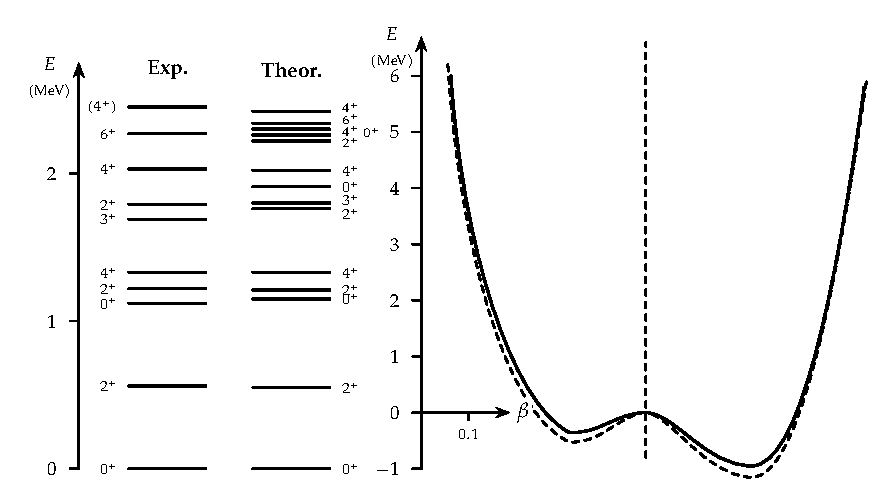
\includegraphics[width=0.75\textwidth]{pictures/9_4}
\par\end{centering}
\caption{\label{fig:9.4}$^{76}\text{Se}$ 的实验能级与唯象玻色子 Hamiltonian 本征值的对比。实线表示本征
$\beta\text{-}\gamma$ 坐标系在 $\gamma=0^{\circ}$ 时的势能曲线；虚线给出了源自微观自洽计算的势能曲线（引自
\cite{LH75}）。}
\end{figure}

通过在 Hamiltonian 中恰当选择参数，人们还能够平滑地描述从球形振动谱、经由中等非谐性、直至具有清晰转动能带结构的能谱相变演化
\cite{Ho70,GMG69,GMG70,DB70,GG71,Ho71a}。一旦有效势能 $V(Q)$ 具有极其深邃且明确的非零形变极小值，转动能带结构便会自然涌现（参见图
9.5）。然而在那些强烈形变的情形下，为了达到计算收敛，必须引入极其庞大数目的玻色子（多达 30 个声子）。除了高阶玻色子分量所带来的巨大数值计算开销之外，在物理层面上也难免令人产生深刻疑虑，因为如此庞大的声子数目极度强烈地违背了
Pauli 原理，而唯象 Hamiltonian 是否真正恰当地体现了这一基本量子禁戒在微观上是不清楚的。

多年来，核物理学界发展出了大量基于唯象群论技术的代数模型，它们的对角化借助成熟的李代数表示理论得到了极大的简化（参见例如 \cite{HNL70,DDK70,VNR75,RD76,RGB77}）。其中最著名、影响最深远的当属相互作用玻色子模型（Interacting
Boson Model, IBM，亦称 $SU(6)$ 模型），它最早由 Janssen 等人提出 \cite{JJD74}，随后由
Arima 和 Iachello 进行了极其系统深入的奠基性研究 \cite{AI75a,AI75b}。它的六个基本构件是五个具有角动量
2 的四极玻色子 $d^{\dagger}_{\mu}$（$\mu=-2,\ldots,+2$）和一个具有单态标量对称性的配对玻色子
$s^{\dagger}$。该模型保持总玻色子数严格守恒，属于 \ref{subsec:9.2.7_=0057FA=004E8Epp-=0073BB=008272=005B50=007684=0065B9=006CD5}
中所讨论的 Schwinger 类型的 pp-玻色子表象。其具有 Hermite 性的有效 Hamiltonian 形式如下：
\begin{align}
H=\epsilon_{s}s^{\dagger}s & +\epsilon_{d}[d^{\dagger}d]_{0}+\sum_{L=0,2,4}c_{L}[[d^{\dagger}d^{\dagger}]_{L}[dd]_{L}]_{0}+u_{0}s^{\dagger}s^{\dagger}ss\nonumber \\
 & +\left\{ v_{2}[[d^{\dagger}d^{\dagger}]_{2}[ds]_{2}]_{0}+v_{0}[d^{\dagger}d^{\dagger}]_{0}ss+u_{2}[[d^{\dagger}s^{\dagger}]_{2}[ds]_{2}]_{0}+\text{h.c.}\right\} .\label{eq:9.119}
\end{align}
它包含八个自由唯象参数 $\epsilon=\epsilon_{d}-\epsilon_{s},c_{0},c_{2},c_{4},u_{0},u_{2},v_{0},v_{2}$，这些参数通常由实验数据拟合确定。此外，我们还需要两个额外的耦合常数来定义电四极跃迁算符：
\begin{equation}
T_{2\mu}=q_{0}\left([d^{\dagger}s]_{2\mu}+\text{h.c.}\right)+q_{1}[d^{\dagger}d]_{2\mu}.\label{eq:9.120}
\end{equation}
在相互作用完全消失的平庸极限下（$c_{L}=v_{L}=u_{L}=0$），体系的基态纯粹由 $s$ 玻色子的凝聚所构成：
\[
|0)=\frac{1}{\sqrt{n!}}(s^{\dagger})^{n}|-\rangle,
\]
其中 $|-\rangle$ 代表裸真空，$2n$ 是核子总数。通过相继将一个或若干个 $s$ 玻色子替换为 $d$ 玻色子，我们在同一原子核中获得具有确定激发能量
$\epsilon=\epsilon_{d}-\epsilon_{s}$ 的四极集体激发态：
\[
|\mu)=\frac{1}{\sqrt{(n-1)!}}d^{\dagger}_{\mu}(s^{\dagger})^{n-1}|-\rangle.
\]
因此，其无微扰能谱展现为如图 1.5 所示的纯粹简谐四极多重态谱。继续添加更多的 $s$ 玻色子，我们便能如 Seniority
模型（参见 \ref{sec:8.2_Tamm-Dancoff=008FD1=004F3C}）所讨论的那样，自然跨越并描述具有核子数
$2n+2,2n+4,\ldots$ 的邻近偶偶核的能谱。

玻色子之间的相互作用项在体系中诱导了丰富的多体关联。此时必须在包含 $n_{s}$ 个 $s$ 玻色子与 $n_{d}=n-n_{s}$
个 $d$ 玻色子的多玻色子基底 $|n_{s},n_{d},\alpha)$ 中对角化 Hamiltonian（式 9.119）（$\alpha$
包含唯一确定该态所需的所有其余量子数）。利用群论张量代数方法，相关矩阵元的计算得到了极大的简化。

总玻色子数守恒关系式
\[
n=\hat{n}_{s}+\hat{n}_{d}=s^{\dagger}s+\sum_{\mu}d^{\dagger}_{\mu}d_{\mu}
\]
可被直接用于完全消去算符 $s$ 与 $s^{\dagger}$。对于固定的核子总数 $n$，基底态矢量完全由 $d$ 玻色子的量子数所表征，只要我们将湮灭算符
$s$ 形式替换为
\begin{equation}
s\to\sqrt{n-\sum_{\mu}d^{\dagger}_{\mu}d_{\mu}},\label{eq:9.121}
\end{equation}
便能严格保证 Hamiltonian 矩阵元的守恒。例如我们有：
\begin{align*}
s|n_{s}=n-n_{d},n_{d},\alpha) & =\sqrt{n_{s}}|n-n_{d}-1,n_{d},\alpha)\\
 & =\sqrt{n-\sum_{\mu}d^{\dagger}_{\mu}d_{\mu}}\,|n-n_{d}-1,n_{d},\alpha).
\end{align*}
将这一代换法则应用于算符（式 9.119），我们最终获得了一个仅包含四极玻色子 $d^{\dagger}_{\mu}$ 的有效 Hamiltonian。然而，它不再保持玻色子数守恒，并且通过对式
\ref{eq:9.121} 中的平方根进行 Taylor 展开，我们会得到包含无穷阶 $d^{\dagger}d\cdots$
的幂级数。这正是 $SU(6)$ 模型的 Holstein-Primakoff 版本 \cite{JJD74}。因此，引入 $s$
玻色子是一种极其精妙的代数工具，它通过将 Pauli 原理引入的非线性平方根因子代数化，巧妙地构建出了严格有限阶截断的代数玻色子表象。我们必须澄清的是：对于固定的粒子数而言，$s$
玻色子并没有引入任何新的物理自由度，它仅仅是用来构建无微扰基态的辅助算符；该模型并不包含 8.3.5 节所讨论的 $2p\text{-}2h$
类型的 $0^{+}$ 配对振动。另一方面，$s$ 玻色子的引入允许人们在一个统一的代数框架下系统处理相邻的 $A+2,A+4,\ldots$
原子核基态与激发态。

取决于模型参数的具体取值，相互作用玻色子模型拥有若干重要的动力学对称性极限，它们对应于 $SU(6)$ 的不同子群链分解 \cite{CCF79}，并且在很多情况下能够给出优美的解析严格解。这些代数对称极限在实际原子核的集体激发分类中扮演着极其关键的角色：
\begin{enumerate}
\item \textbf{Seniority 极限（$SU(2)$ 对称性）}：当 $c_{L}=v_{L}=0,u_{2}=0$（即完全切断与
$d$ 玻色子的耦合）时，我们精确重现了 \ref{sec:6.2_Seniority=0065B9=006848} 中所讨论的单
$j$-壳层的 Seniority 方案：
\[
H=\epsilon_{s}s^{\dagger}s+u_{0}s^{\dagger}s^{\dagger}ss=-GS_{+}S_{-},
\]
相应的准自旋算符为：
\[
S_{+}=\sqrt{\Omega}s^{\dagger}\sqrt{1-\frac{s^{\dagger}s}{\Omega}},
\]
且参数对应关系为 $u_{0}=-G,\epsilon_{s}=G\cdot\Omega$。
\item \textbf{振动极限（$SU(5)$ 对称性）} \cite{AI76}：在弱相互作用极限下（$u_{L}=0;v_{L},c_{L}\ll\epsilon_{d}-\epsilon_{s}$），体系展现出
$SU(5)$ 振动动力学对称性。此时 $s$ 玻色子不发挥动态作用，在极限情况下我们仅有相互作用四极玻色子（参见 \cite{BTK65,DDK70,IA74}）：
\begin{equation}
H=\sum_{\mu}\epsilon_{d}d^{\dagger}_{\mu}d_{\mu}+\sum_{L=0,2,4}c_{L}[[d^{\dagger}d^{\dagger}]_{L}[dd]_{L}]_{0}.\label{eq:9.122}
\end{equation}
其所有本征能级和跃迁几率均能以严格解析闭合形式显式给出。
\item \textbf{转动极限（$SU(3)$ 对称性）} \cite{AI78a}：若模型的各项参数之间满足特定比值关系，Hamiltonian（式
9.119）可以被改写为角动量与四极张量算符标量积的形式：
\begin{equation}
H=\epsilon\sum_{\mu}d^{\dagger}_{\mu}d_{\mu}-\kappa'[\boldsymbol{L}\cdot\boldsymbol{L}]_{0}-\kappa[\boldsymbol{Q}\cdot\boldsymbol{Q}]_{0},\label{eq:9.123}
\end{equation}
其中包含常数 $\epsilon,\kappa,\kappa'$，三个角动量算符分量
\[
L_{\mu}=\sqrt{10}[d^{\dagger}d]_{1\mu},
\]
以及五个内禀四极算符
\[
Q_{\mu}=d^{\dagger}_{\mu}s+s^{\dagger}d_{\mu}-\frac{\sqrt{7}}{2}[d^{\dagger}d]_{2\mu}.
\]
当 $\epsilon=\kappa'=0$ 时，我们得到了建立在 $SU(3)$ 李代数之上的纯转动极限。这是费米子体系中著名的
Elliott 模型 \cite{El58} 的玻色子推广，其优良群论性质在文献中被广泛探讨 \cite{Ha68,Ve68,JDJ75}。该极限精确再现了轴对称刚性转子的能谱规律（伴随简并的
$2^{+}_{\beta}$ 与 $2^{+}_{\gamma}$ 能级）：
\[
E(\lambda,\mu,K,L,M)=\frac{3}{4}(\kappa-\kappa')L(L+1)-\kappa\left[\lambda^{2}+\mu^{2}+\lambda\mu+3(\lambda+\mu)\right],
\]
其中 $(\lambda,\mu,K,L,M)$ 是 $SU(3)$ 群的一整套特征量子数。
\item \textbf{$\gamma$-非稳定软振子极限（$O(6)$ 对称性）} \cite{AI78b,CC78,CBP78}：在各大主壳层即将填满的末端，$SU(6)$
的另一个重要子群 $O(6)$ 在原子核低激发能谱的分类中发挥了举足轻重的作用。在此极限下，全部能级本征值同样能够以简洁的代数形式给出。在特定的物理极限下，其数学解与著名的完全
$\gamma$-软形变谐振子模型——即 Wilets-Jean 模型 \cite{WJ56,Me78}——完全重合。
\end{enumerate}
由于 $SU(6)$ 相互作用玻色子模型有机地熔铸了如此多深刻的微观集体物理效应，且拥有多达 11 个可调的有效相互作用参数，因此在拟合球形核、弱形变过渡核乃至强形变核的大量实验能谱与电磁跃迁时均取得了无可争辩的巨大成功
\cite{Ia77,AOI78,Ia78}。在单 $j$-壳层配对加四极相互作用框架下，人们也已经给出了该模型坚实的微观理论论证
\cite{OAI78}。然而，一个包含完整单核子自由度及其微观耦合的完备微观推导，至今仍然是核理论中极具挑战性的前沿课题。

\subsubsection{微观计算\label{subsubsec:9.2.8.2_=005FAE=0089C2=008BA1=007B97}}

尽管唯象玻色子模型在拟合实验能谱和电磁跃迁几率方面取得了令人瞩目的辉煌成功，但只要缺乏直接的微观微商，我们就永远无法在逻辑上排除如下担忧：这些模型是否仅仅是通过对若干自由参数的人工精细微调，从而在数学上“模拟”了某些与真正玻色子动力学毫不相干的其他微观物理机制。因此，在核多体玻色理论的构建中，最为根本的基石在于严格证明：进入玻色子有效
Hamiltonian 的全部展开参数，在原则上都可以从微观的多体相互作用 Hamiltonian 中自洽推导出来。

Lee 和 Holzwarth \cite{LH75} 率先将基于集体玻色子的 Marumori 方法（\ref{subsec:9.2.4_Marumori=0073BB=008272=005C55=005F00}）应用于具有相当纯粹四极结构的非谐核体系中。他们将表面
$\delta$ 相互作用（式 4.117）的微观多体 Hamiltonian 在角动量为 2 的 TDA 集体玻色子基底上展开至第四阶，发现计算得到的有效展开系数
$h_{lm}$（式 9.117）与实验拟合所得参数展现出了令人信服的高度一致性 \cite{HL72a}。图 9.4 中的虚线直观地展示了以此方式微观计算出的玻色子有效势能曲线
$V(Q)$。

B. Sørensen 广泛采用了 \ref{subsubsec:9.2.3.2_=009650=005236=005728=005C11=006570=0096C6=004F53=0073BB=008272=005B50=0060C5=005F62}
中所论述的 Belyaev-Zelevinski 截断代数方法。在系列经典文献中 \cite{So67,So68a,So68b,So69,So70}，他系统探讨了闭壳附近的配对振动模式以及过渡区原子核中的四极振动模式。他采用经过轻微唯象修正的配对加四极相互作用（式
4.141），将微观多体 Hamiltonian 推进至四阶展开，不仅在半定量层面上成功再现了这些原子核的核心物理特征，而且揭示了其微观演化规律。然而，在集体模式与非集体的双准粒子单粒子态之间的动力学耦合变得不可忽略的情形下，该方法遇到了一定困难。

更为完备与深刻的微观微商计算由 Kishimoto 和 Tamura 彻底完成 \cite{KT72,KT76}。除了标准的单极配对加四极相互作用之外，他们还在微观相互作用中显式引入了四极配对力（式
4.134），并在 $I=2$ 的集体玻色子分支上将微观 Hamiltonian 系统展开至第六阶。他们的深入研究揭示：在许多过渡核中，集体分支与非集体分支之间的耦合至关重要。为了微观处理这种混合，他们引入了
Feshbach 投影算符形式体系 \cite{Fe58,Fe62}，从而在集体子空间中导出了包含能量依赖性的重整化有效相互作用参数
$\tilde{h}_{lm}$。这些极其艰深复杂的微观自洽计算不仅在近球形振动核中，而且在复杂的过渡核乃至具有良好转动特征的强形变核中，均展现出了与实验能谱及跃迁几率异乎寻常的绝佳吻合。图
9.5 展示了稀土区钐（Sm）同位素链从球形向稳定形变过渡的相变过程的经典微观计算成果，表 9.1 则列出了相应的电四极跃迁及光谱四极矩的对比数据。

\begin{figure}[H]
\begin{centering}
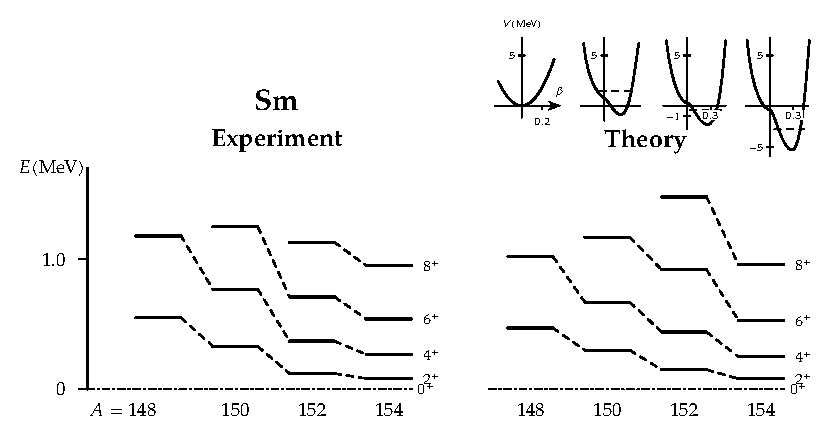
\includegraphics[width=0.85\textwidth]{pictures/9_5}
\par\end{centering}
\caption{\label{fig:9.5}钐（Sm）同位素核中从球形到形变的相变。能谱结构从纯振动态逐渐转变为规则的转动态。图中上方还给出了玻色子
Hamiltonian 随形变参数 $\beta$ 变化的相应微观有效势能曲线（引自 \cite{KT76}）。}
\end{figure}

\begin{table}[H]
\caption{\label{tab:9.1}利用微观玻色展开方法计算的第一激发 $2^{+}$ 态的光谱四极矩与 $B(E2)$ 跃迁值，并与实验测量数据进行对比（引自
\cite{TK73}）。}

\centering{}%
\begin{tabular}{|c|c|c|c|c|}
\hline 
 & \multicolumn{2}{c|}{$Q_{2^{+}}$ {[}$e\cdot\text{b}${]}} & \multicolumn{2}{c|}{$B(E2;2^{+}\to0^{+})$ {[}$e^{2}\cdot\text{b}^{2}${]}}\tabularnewline
\hline 
 & 实验值 & 理论值 & 实验值 & 理论值\tabularnewline
\hline 
$^{148}\text{Sm}$ & $-0.97\pm0.27$ & $-0.91$ & $0.141\pm0.005$ & $0.152$\tabularnewline
$^{150}\text{Sm}$ & $-1.31\pm0.19$ & $-1.17$ & $0.274\pm0.006$ & $0.270$\tabularnewline
$^{152}\text{Sm}$ & $-1.73\pm0.20$ & $-1.72$ & $0.666\pm0.014$ & $0.697$\tabularnewline
$^{154}\text{Sm}$ & $-1.91$ & $-1.91$ & $0.922\pm0.040$ & $0.884$\tabularnewline
\hline 
\end{tabular}
\end{table}


\section{奇 A 核与粒子-振动耦合\label{sec:9.3_=005947A=006838=004E0E=007C92=005B50-=00632F=0052A8=008026=005408}}

前文各节主要局限于由偶数个费米子所构成的原子核体系。显而易见，具有奇数质量数（奇 A）的原子核体系同样普遍存在着丰富的集体激发态。在核物理发展史上，最著名的代表性范例当属
$^{209}\text{Bi}$ 的微观七重态（septuplet）：在该核中，处于 $1h_{9/2}$ 单质子轨道上的奇价质子与双闭壳核芯
$^{208}\text{Pb}$ 在 $2.61\text{ MeV}$ 处的 $3^{-}$ 八极集体振动声子发生耦合。由于该奇质子对核芯集体振动仅产生极其微弱的微扰，从而在
$2.61\text{ MeV}$ 激发能附近诱导产生了一个能级劈裂极小（仅约数百 $\text{keV}$）的七重能级组态（角动量分别为
$3/2^{+},5/2^{+},7/2^{+},9/2^{+},11/2^{+},13/2^{+},15/2^{+}$；参见图
9.6）。在理论上，此类状态通常在粒子-振动耦合（particle vibration coupling, PVC，或 VPC）模型框架下处理
\cite{BM75}。事实表明，该模型在微观本质上与奇核系统的玻色展开方法紧密相连。

\begin{figure}[H]
\begin{centering}
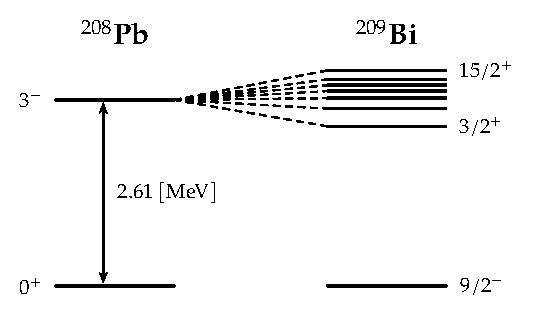
\includegraphics[width=0.7\textwidth]{pictures/9_6}
\par\end{centering}
\caption{\label{fig:9.6}$^{208}\text{Pb}$ 与 $^{209}\text{Bi}$ 实验激发能谱的示意性对比。}
\end{figure}


\subsection{奇 A 系统的玻色展开\label{subsec:9.3.1_=005947A=007CFB=007EDF=007684=0073BB=008272=005C55=005F00}}

前一节所考察的所有各类玻色子表象理论，均可系统推广至奇质量核体系 \cite{Ya65,DJ73,Ma73,Ma74,Pr74,RS77a,BM78}。由于其基本指导原则与偶偶核情形并无本质差异，在此我们仅简要勾勒
Belyaev-Zelevinski 方法与 Dyson 方法的核心框架。

在 Belyaev-Zelevinski 方法中，除了双费米子对算符 $b^{\dagger}_{\mu},a_{\mu\nu}$
{[}式 9.24 与式 9.25{]} 之外，我们现在还必须显式计入单费米子算符 $\alpha^{\dagger}_{k}$，并将所有这些算符统一映射到一个扩充的乘积空间中，即通常的
$B^{\dagger}_{\mu}$ 玻色子空间与由一个同玻色子完全对易的\textbf{理想费米子}（ideal fermion）$\beta^{\dagger}_{k}$
所张成的空间的直积：
\begin{equation}
[B_{\mu},\beta^{\dagger}_{k}]=[B^{\dagger}_{\mu},\beta^{\dagger}_{k}]=0.\label{eq:9.124}
\end{equation}
由于在同一时刻至多只允许存在一个理想费米子，因此算符 $\beta_{k}$ 满足代数关系 \cite{Ok74}：
\begin{equation}
\beta_{k}\beta_{l}=\beta^{\dagger}_{k}\beta^{\dagger}_{l}=0,\qquad\beta_{k}\beta^{\dagger}_{l}=\delta_{kl}.\label{eq:9.125}
\end{equation}
该扩充乘积空间中的真空投影算符由下式给出：
\begin{equation}
|0)(0|={:}\exp\left(-\sum_{\mu}B^{\dagger}_{\mu}B_{\mu}\right){:}\left(1-\sum_{k}\beta^{\dagger}_{k}\beta_{k}\right),\label{eq:9.126}
\end{equation}
这再次确切意味着：
\begin{equation}
B_{\mu}|0)=\beta_{k}|0)=0.\label{eq:9.127}
\end{equation}
于是，直积空间中的一组标准正交基底为：
\begin{equation}
|k,N)=\mathscr{N}_{B}\cdot\beta^{\dagger}_{k}B^{\dagger}_{\mu_{1}}\cdots B^{\dagger}_{\mu_{N}}|0),\qquad N=0,1,\ldots\label{eq:9.128}
\end{equation}
除了算符 $b^{\dagger}_{\mu}$ 与 $a_{\mu\nu}$ 的对易代数（式 9.27）之外，我们现在还必须考虑单费米子算符之间以及单费米子与对算符之间的反对易和对易关系：
\begin{align}
\{\alpha_{k},\alpha_{l}\} & =\{\alpha^{\dagger}_{k},\alpha^{\dagger}_{l}\}=0,\qquad\{\alpha_{k},\alpha^{\dagger}_{l}\}=\delta_{kl},\nonumber \\{}
[\alpha_{k},b_{\mu}] & =0,\qquad[\alpha_{k},b^{\dagger}_{\mu}]=\sum_{l}C^{\mu}_{kl}\alpha^{\dagger}_{l},\label{eq:9.129}\\{}
[\alpha_{k},a_{\mu\nu}] & =\sum_{l}\Gamma^{\mu k}_{\nu l}\alpha_{l},\nonumber 
\end{align}
其中 $\Gamma^{\mu k}_{\nu l}$ 由式 \ref{eq:9.29} 所定义。

现在我们仿照 \ref{subsubsec:9.2.3.1_=005FAE=006270=0073BB=008272=005C55=005F00}
的思路，对各物理算符在玻色子空间中的像做出如下展开拟设（选取该特定拟设形式的深入讨论参见 \cite{Ma74}）；在此我们只需指出，这些展开在微扰意义下逐阶精确满足上述对易规则\footnote{在非集体情形下，类似于式 9.103，我们可以对 $(b^{\dagger}_{kl})_{B}$ 与 $(\alpha^{\dagger}_{k})_{B}$
的无穷级数进行显式封闭求和：
\begin{align*}
(a_{kl})_{B} & =\sum_{r}B^{\dagger}_{lr}B_{kr}+\beta^{\dagger}_{l}\beta_{k},\\
(b^{\dagger}_{kl})_{B} & =\left(B^{\dagger}\sqrt{1-B^{\dagger}B}\right)_{kl}+\sum_{pq}\left[\left(\sqrt{1-B^{\dagger}B}\right)_{pq}B^{\dagger}_{kl}\right]\beta^{\dagger}_{p}\beta_{q},\\
(\alpha^{\dagger}_{k})_{B} & =\sum_{l}\left(\sqrt{1-B^{\dagger}B}\right)_{lk}\beta^{\dagger}_{l}+B^{\dagger}_{kl}\beta_{l}.
\end{align*}
}：
\begin{align}
(a_{\mu\nu})_{B} & =\sum_{\rho\sigma}\Gamma^{\mu\rho}_{\nu\sigma}B^{\dagger}_{\rho}B_{\sigma}+\sum_{kl}\Gamma^{\mu k}_{\nu l}\beta^{\dagger}_{k}\beta_{l},\nonumber \\
(b^{\dagger}_{\mu})_{B} & =B^{\dagger}_{\mu}-\frac{1}{4}\sum_{\nu\rho\sigma}\Gamma^{\nu\rho}_{\mu\sigma}B^{\dagger}_{\nu}B^{\dagger}_{\rho}B_{\sigma}+\cdots-\frac{1}{2}\sum_{\nu kl}\Gamma^{\nu k}_{\mu l}B^{\dagger}_{\nu}\beta^{\dagger}_{k}\beta_{l}+\cdots,\label{eq:9.130}\\
(\alpha^{\dagger}_{k})_{B} & =\beta^{\dagger}_{k}-\frac{1}{2}\sum_{\rho\sigma l}\Gamma^{\rho l}_{\sigma k}B^{\dagger}_{\rho}B_{\sigma}\beta^{\dagger}_{l}+\cdots+\sum_{\rho l}C^{\rho}_{kl}B^{\dagger}_{\rho}\beta_{l}.\nonumber 
\end{align}
借助这些算符展开式，我们便能直接构建出多体微观 Hamiltonian（式 9.32）在直积空间中的玻色子-费米子对应像。

\subsection{粒子-振动耦合（Bohr）Hamiltonian 的推导\label{subsec:9.3.2_=007C92=005B50-=00632F=0052A8=008026=005408Hamiltonian=007684=0063A8=005BFC}}

将式 \ref{eq:9.130} 代入 Hamiltonian（式 9.32 与 9.33）中，如果我们暂时忽略基态关联（即假定
$H^{40}=0$\footnote{由于忽略了 $H^{40}$，形如 $B^{\dagger}B^{\dagger}$ 与 $BB$ 的项暂时缺失。通过变换到
RPA 玻色子（参见附录 E.5），$B_{\mu}=\sum_{mi\rho}C^{\mu*}_{mi}(X^{\rho}_{mi}Q_{\rho}+Y^{\rho*}_{mi}Q^{\dagger}_{\rho})$，我们完全可以将它们自然计入。}），则在关于 $\Gamma$ 的一阶近似下可得：
\begin{align}
H & =\sum_{\mu}\Omega_{\mu}B^{\dagger}_{\mu}B_{\mu}+\sum_{k}E_{k}\beta^{\dagger}_{k}\beta_{k}+\cdots+H_{\text{coupl}},\nonumber \\
H_{\text{coupl}} & =\sum_{\mu,k,l}\frac{1}{2}\left(\gamma^{\mu}_{kl}B^{\dagger}_{\mu}\beta^{\dagger}_{k}\beta_{l}+\text{h.c.}\right)\label{eq:9.131}\\
 & \quad-\frac{1}{2}\sum_{\substack{\mu\nu\lambda\\
kl
}
}V^{22}_{\mu\nu}\left(\Gamma^{\lambda l*}_{\nu k}B^{\dagger}_{\mu}B_{\lambda}+\Gamma^{\lambda k}_{\mu l}B^{\dagger}_{\lambda}B_{\nu}\right)\beta^{\dagger}_{k}\beta_{l},\nonumber 
\end{align}
其中微观单粒子-振动耦合顶点定义为：
\begin{equation}
\gamma^{\mu}_{kl}=2\sum_{rs}H^{31}_{rskl}C^{\mu*}_{rs},\label{eq:9.132}
\end{equation}
这里的 $C^{\mu}_{rs}$ 是 TDA 振幅，$\Omega_{\mu}$ 是相应的本征能量。在式 \ref{eq:9.131}
中，我们略去了包含两个 $\Gamma$ 的 $B^{\dagger}B$ 项，因为它们通常远小于仅含单一 $\Gamma$
的主导项。耦合 Hamiltonian $H_{\text{coupl}}$ 中的第一项在核物理文献中被称为 \textbf{Bohr
耦合 Hamiltonian} \cite{BM75}，因为它最初是在唯象液滴模型中被推导出来的（参见 \ref{subsec:9.3.4_=007C92=005B50-=00632F=0052A8=008026=005408=009876=0070B9=007684=006027=008D28}）。而
$H_{\text{coupl}}$ 中的第二项则源自玻色展开的系统性微观推导，正如我们后文将阐明的，它在微观上精确起到了修正 Pauli
原理的作用。

对于具有时间反演不变性的多体系统，矩阵元 $H^{31}_{rskl}$ 可以在正则单粒子基底（参见第 7 章）中根据式 E.25
显式计算得出：
\begin{align}
H^{31}_{rskl}=\frac{1}{3}\cdot\frac{1}{4} & \left\{ -\bar{v}_{r\bar{k}\bar{s}l}\left(\eta^{+}_{rs}\xi^{+}_{kl}+\eta^{-}_{rs}\xi^{-}_{kl}\right)\right.\nonumber \\
 & \quad+\bar{v}_{sk\bar{r}l}\left(\eta^{+}_{rs}\xi^{+}_{kl}-\eta^{-}_{rs}\xi^{-}_{kl}\right)\label{eq:9.133}\\
 & \quad\left.+\bar{v}_{r\bar{s}\bar{k}l}\left(\xi^{+}_{rs}\eta^{+}_{kl}-\xi^{-}_{rs}\eta^{-}_{kl}\right)\right\} ,\nonumber 
\end{align}
其中占据因子 $\xi,\eta$ 的定义见式 8.202。

在下文中，我们将更加深入地考察不存在超流配对关联的核系统。此时，准粒子算符 $\beta^{\dagger}_{k}$ 必须替换为真实的单粒子产生算符
$c^{\dagger}_{m}$ 或单空穴产生算符 $c_{i}$（我们用指标 $m,n$ 表示粒子态，用 $i,j$ 表示空穴态；参见第
2 章）。准粒子能量相应地被单粒子能量 $\epsilon_{m}$ 或空穴能量 $-\epsilon_{i}$ 所替代（能量零点取为
$\epsilon_{F}=0$）。由于在一般的准粒子形式体系中我们既可以表示粒子-空穴振动（指标 $\nu,\nu',\ldots$），也可以表示粒子-粒子（或空穴-空穴）振动（指标
$\tau,\tau',\ldots$），因此我们自然获得两类耦合顶点。忽略配对关联，当我们考虑一个粒子耦合到一个 $1p\text{-}1h$
激发态时（注意到原始振幅 $C^{\mu}_{rs}$ 是反对称的），$H_{\text{coupl}}$ 的第一项显式写为：
\begin{align}
H_{\text{coupl}} & =\frac{1}{3}\sum_{\nu}\sum_{mn}\sum_{m'i'}C^{\nu*}_{m'i'}\bar{v}_{m'mi'n}B^{\dagger}_{\nu}c^{\dagger}_{m}c_{n}+\text{h.c.}\nonumber \\
 & \quad-\frac{1}{3}\cdot\frac{1}{2}\sum_{\tau}\sum_{jn}\sum_{m'n'}C^{\tau*}_{m'n'}\bar{v}_{m'n'jn}B^{\dagger}_{\tau}c_{j}c_{n}+\text{h.c.}\label{eq:9.134}
\end{align}
因子 $1/3$ 的出现，本质上是因为我们的“费米子-玻色子”乘积基底比原始费米子基底整整放大了三倍——它包含了将粒子耦合到 ph
振动的两种独立可能方式，以及将空穴耦合到 pp 振动的一种可能方式（另见后文）。利用图线规则（第 8 章与附录 F），我们可以将两个耦合顶点
$\gamma^{\nu}_{mn}$ 与 $\gamma^{\tau}_{jn}$ 形象地用图 9.7 表示出来。

\begin{figure}[H]
\begin{centering}
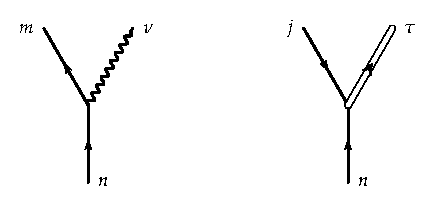
\includegraphics[width=0.65\textwidth]{pictures/9_7}
\par\end{centering}
\caption{\label{fig:9.7}单粒子耦合到单粒子加 ph 振动的相互作用顶点，以及单粒子耦合到单空穴加 pp 振动的相互作用顶点。}
\end{figure}

为了使讨论更加集中明晰，我们暂时忽略激发 pp 振动的可能性，即式 \ref{eq:9.134} 中的第二项自动掉落。在此物理假设下，式
\ref{eq:9.134} 中的加权因子 $1/3$ 相应地变为 $1/2$，即\footnote{我们在此处所使用的相互作用在形式上是原始的裸两体相互作用，正如迄今为止所有玻色展开理论一样。然而可以证明（参见附录 F），顶点（式
9.135）中的裸相互作用可以被不一定严格反对称的有效粒子-空穴相互作用所替代。}：
\begin{equation}
H_{\text{coupl}}=\frac{1}{2}\sum_{\nu}\left(\gamma^{\nu}_{mn}B^{\dagger}_{\nu}c^{\dagger}_{m}c_{n}+\text{h.c.}\right),\label{eq:9.135}
\end{equation}
其中 $\gamma^{\nu}_{kl}=\sum_{mi}C^{\nu*}_{m'i'}\bar{v}_{m'ki'l}$。

为了处理奇核的集体振动激发，我们形式上必须在多声子-单粒子基底（式 9.128）中对角化总 Hamiltonian（式 9.131）。在实际操作中，通常只需计及一个核心声子（如四极声子或八极声子）。偶偶核底层振子的非谐性越显著，在
Hamiltonian 的对角化中所需的多声子基底组态就越庞大。这一路线在 Alaga 及其合作者所发展的唯象模型中得到了长期的贯彻与应用
\cite{Al67,APS75}。正如我们在偶偶核中所看到的，玻色子描述对于转动核同样行之有效。因此，Hamiltonian（式
9.131）在原则上有能力系统描述当一个奇价粒子耦合到变形转子时所引发的所有微观物理效应，例如转动顺排（rotational alignment）或非轴对称三轴形变特征
\cite{AP76,PVD77}。然而在实际应用中，该 Hamiltonian 主要是针对近简谐振动核开展研究的，我们接下来就转向微扰论讨论。

\subsection{粒子-振动耦合（微扰论）\label{subsec:9.3.3_=007C92=005B50-=00632F=0052A8=008026=005408=00FF08=005FAE=006270=008BBA=00FF09}}

Hamiltonian（式 9.131）极适用于处理奇核中的集体振动。在最简单的情形下，我们将相邻的偶偶核视为纯简谐振子，此时体系的第一个集体激发态便是单粒子-振动声子耦合态。此外，在很多实际核中，粒子-振动耦合（PVC）非常微弱，使得
$H_{\text{coupl}}$ 完全可以在定态微扰论的框架下处理（即弱耦合情形）。

若我们要计算单粒子-振动状态由于耦合项所导致的能量位移，二阶微扰展开给出：
\begin{align}
\Delta E & =\Delta E_{1}+\Delta E_{2}\nonumber \\
 & =(p\mu|H_{\text{coupl}}|p\mu)+\sum_{\substack{kN\\
\ne p\mu
}
}\frac{(p\mu|H_{\text{coupl}}|kN)(kN|H_{\text{coupl}}|p\mu)}{E_{p\mu}-E_{kN}},\label{eq:9.136}
\end{align}
其中 $|p\mu)=\beta^{\dagger}_{p}B^{\dagger}_{\mu}|0)$ 代表未受微扰的单粒子加单声子组态，中间态
$|kN)$ 定义见式 \ref{eq:9.128}。在一阶微扰中，只有 $H_{\text{coupl}}$ 的第二项产生非零贡献，由式
\ref{eq:9.33}、\ref{eq:9.26} 与 \ref{eq:9.131} 可得：
\begin{align}
(p\mu|H_{\text{coupl}}|p\mu) & =-\frac{1}{2}\sum_{\nu}\left(V^{22}_{\mu\nu}\Gamma^{\mu p}_{\nu p}+\text{c.c.}\right)\nonumber \\
 & =-\frac{1}{4}\sum_{klq}\left(H^{22}_{klpq}C^{\mu*}_{kl}C^{\mu}_{pq}+\text{c.c.}\right).\label{eq:9.137}
\end{align}
在文献中，另一种与当前讨论密切相关的方法是 Bohr 与 Mottelson 提出的\textbf{核场论}（Nuclear Field
Theory, NFT）\cite{Mo67,BM75}，随后由 Broglia 等人进行了极其详尽的发展和系统应用 \cite{BBB77}。为了便于将本章表述与
NFT 进行精确比对，我们引入一条规则：每当 TDA 振幅（如式 9.137 中的 $C^{\mu}_{pq}$）的两个指标不汇合到同一个矩阵元且未被同时求和时，我们就必须利用
TDA 方程（式 8.10），从而使这类振幅变换为两个指标均作用在同一个 $\bar{v}$ 上并被闭合求和的形式。将此规则应用于一阶表达式（式
9.137）并在 HF 极限下将其严格局限于 ph 振动，我们得到：
\begin{equation}
\Delta E_{1}=-\sum_{i}\frac{|\gamma^{\mu}_{ip}|^{2}}{\Omega_{\mu}-\epsilon_{p}+\epsilon_{i}}.\label{eq:9.138}
\end{equation}
在二阶微扰中，只有 $H_{\text{coupl}}$ 的第一项做出贡献。它来源于包含零个玻色子（$N=0$）与两个玻色子（$N=2$）的中间态
$|kN)$。在 HF 极限下，该二阶项显式为\footnote{严格执行微扰论（式 9.136）对各项所给出的权重因子，与我们在此写出的形式略有不同（例如式 9.139 中的第一项原本会带有一个
$1/2$ 因子）。然而极为精妙的一点是：在对角化式 9.131 中的第二项时（即将其微扰级数求和至无穷阶），会产生与式 9.139
完全相同结构的额外修正项，将它们合并后恰好消去了 $1/2$ 因子。这一加权因子的微观来源在历史上曾引发了长期的争论 \cite{JDK69,El70}。简明准则是：在进行完全对角化时必须严格保留因子
$1/2$；而在仅执行最低阶微扰论时，该因子应当被吸收。}：
\begin{equation}
\Delta E_{2}=\sum_{n}\frac{|\gamma^{\mu}_{pn}|^{2}}{\Omega_{\mu}+\epsilon_{p}-\epsilon_{n}}+\sum_{n}\frac{|\gamma^{\mu}_{np}|^{2}}{\epsilon_{p}-\epsilon_{n}-\Omega_{\mu}}.\label{eq:9.139}
\end{equation}
根据图线规则，$\Delta E_{2}$ 的第一项和第二项分别对应于图 9.8 中的图 (a) 与图 (b)，而 $\Delta E_{1}$
则对应于图 (c)。图 9.8(d) 所示的微观过程显式涉及 $H^{40}$ 的两体矩阵元，如果我们一开始就在式 \ref{eq:9.131}
中保留 $H^{40}$ 并变换到 RPA 玻色子，就会自然导出该贡献。略去微小的 RPA 反向振幅，其解析表达式为：
\begin{equation}
\sum_{i}\frac{|\gamma^{\mu}_{pi}|^{2}}{\Omega_{\mu}+\epsilon_{p}-\epsilon_{i}}.\label{eq:9.140}
\end{equation}

\begin{figure}[H]
\begin{centering}
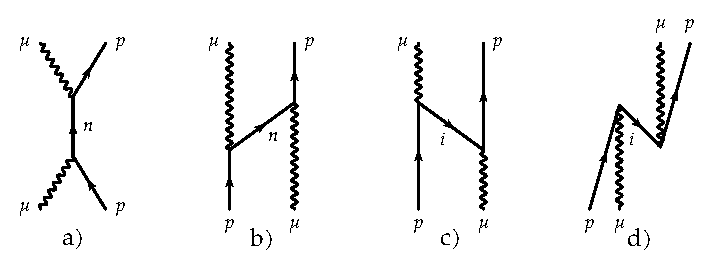
\includegraphics[width=0.75\textwidth]{pictures/9_8}
\par\end{centering}
\caption{\label{fig:9.8}代表单粒子-ph 振动耦合二阶能量贡献的四种可能微观图线。}
\end{figure}

图 9.8 中四种微观过程的物理图像极其清晰直观：
\begin{enumerate}
\item 图 (a)：集体振动声子与入射粒子融合成一个中间单粒子态，随后该中间态再次裂变发射出一个单粒子与一个集体振动声子；
\item 图 (b)：在粒子与集体振动共同传播的过程中，粒子自身虚拟激发一个声子并散射到另一个中间单粒子态上，随后该中间粒子吸收最初入射的振动声子；
\item 图 (c)：入射的集体振动声子虚拟解离为一个粒子-空穴对，其中的空穴随后与最初入射的价粒子复合湮灭，而剩余的激发粒子则重新退激构成出射的振动声子。这在本质上代表了空穴从一个粒子伙伴到另一个粒子的量子交换，因此确切体现了
Pauli 原理的禁戒修正。我们清楚地看到，该项正是源于 $H_{\text{coupl}}$ 中的高阶玻色子修正项；
\item 图 (d)：该过程在拓扑上与图 (a) 完全类似，唯一的关键区别在于中间传播的单粒子态被单空穴态所取代。正如前文所述，该过程直接源于多体系统基态中的两体量子关联。
\end{enumerate}
在文献中，Kisslinger 和 Sorensen \cite{KS63} 等人率先计入了图 (a) 与 (b) 的贡献；而空穴耦合同样具有决定性重要地位这一事实，则由
Hafele 首次明确指出 \cite{Ha67}。Mottelson 系统深入地评述了所有这些微观图线在 $^{209}\text{Bi}$
中单粒子与 $3^{-}$ 声子耦合中的相对重要性 \cite{Mo67}。

\subsection{粒子-振动耦合顶点的性质\label{subsec:9.3.4_=007C92=005B50-=00632F=0052A8=008026=005408=009876=0070B9=007684=006027=008D28}}

在继续深入讨论之前，我们首先详细探讨作为图 9.8 所示全部四个微观物理过程核心构件的耦合顶点 $\gamma^{\mu}_{kl}$（式
9.135）。为此，我们将该顶点变换到连续坐标空间 $\boldsymbol{r}$-表象中：
\begin{align}
\gamma^{\mu}_{kl} & =\int\mathrm{d}^{3}r_{1}\,\mathrm{d}^{3}r_{2}\,\phi_{k}(\boldsymbol{r}_{1})\gamma^{\mu}(\boldsymbol{r}_{1},\boldsymbol{r}_{2})\phi^{*}_{l}(\boldsymbol{r}_{2}),\label{eq:9.141}\\
\gamma^{\mu}(\boldsymbol{r}_{2},\boldsymbol{r}_{4}) & =\sum_{mi}\int\mathrm{d}^{3}r_{1}\,\mathrm{d}^{3}r_{3}\,\bar{v}(\boldsymbol{r}_{1},\boldsymbol{r}_{2},\boldsymbol{r}_{3},\boldsymbol{r}_{4})\phi^{*}_{m}(\boldsymbol{r}_{1})C^{\mu*}_{mi}\phi_{i}(\boldsymbol{r}_{3}).\nonumber 
\end{align}
为了进行定性阐明，我们近似将直接相互作用项视为纯 Wigner 类型的 $\delta$ 力（参见第 4 章）并忽略交换项，从而得到局域顶点形式：
\begin{equation}
\gamma^{\mu}(\boldsymbol{r}_{1},\boldsymbol{r}_{2})=\delta(\boldsymbol{r}_{1}-\boldsymbol{r}_{2})\gamma^{\mu}(\boldsymbol{r}_{1}),\qquad\gamma^{\mu}(\boldsymbol{r})\propto\delta\rho^{\mu}(\boldsymbol{r}),\label{eq:9.142}
\end{equation}
其中 $\delta\rho^{\mu}(\boldsymbol{r})$ 正是 8.3.1 节所详尽讨论的跃迁密度\footnote{在当前的定性讨论中，我们忽略了 RPA 与 TDA 激发振幅之间的细微差异。}。根据能量加权求和规则（参见
8.7.5 节）以及半经典流体模型考量 {[}参见 Tassie 模型，式 8.175{]}，跃迁密度可以用球对称基态密度 $\rho_{0}(r)$
的微商显式表达为：
\begin{equation}
\delta\rho^{\lambda}\propto\lambda r^{\lambda-1}Y_{\lambda0}\cdot\frac{\mathrm{d}\rho_{0}}{\mathrm{d}r}\qquad(\lambda\ne0).\label{eq:9.143}
\end{equation}
因此我们清楚地看到：粒子-振动耦合主要发生在原子核的核表面区域。

考察其与唯象液滴模型（参见 \cite{BM75} 以及第 1 章）之间的内在亲缘关系是极其富有启发的：正如在该模型中通常所假定的那样，对于固定的径向坐标
$r$，微小表面变形下的平均场核势阱 $V(\boldsymbol{r})$ 的等势面由式 1.7 给出 \cite{Ha74a}：
\begin{equation}
r_{\Omega}=r\left(1+\sum_{\lambda\mu}\alpha^{*}_{\lambda\mu}Y_{\lambda\mu}(\Omega)\right).\label{eq:9.144}
\end{equation}
这精确等价于等势面方程：
\begin{equation}
V(r_{\Omega},\Omega)=V_{0}(r),\label{eq:9.145}
\end{equation}
其中 $V_{0}(r)$ 是未形变的球对称中心势。因此对于任意实际坐标 $r_{\Omega}$，我们只需通过坐标尺度缩放即可表示实际势阱：
\begin{equation}
V(r_{\Omega},\Omega)=V_{0}\left[\frac{r_{\Omega}}{1+\sum_{\lambda\mu}\alpha^{*}_{\lambda\mu}Y_{\lambda\mu}(\Omega)}\right].\label{eq:9.146}
\end{equation}
对于微小的表面振动变形，我们展开至形变参数 $\alpha_{\lambda\mu}$ 的一阶（将 $r_{\Omega}$ 记回
$r$）：
\begin{equation}
V(r,\Omega)=V_{0}(r)-r\frac{\mathrm{d}V_{0}(r)}{\mathrm{d}r}\sum_{\lambda\mu}\alpha^{*}_{\lambda\mu}Y_{\lambda\mu}(\Omega)+O(\alpha^{2}).\label{eq:9.147}
\end{equation}
因此，粒子与核表面形变之间的耦合作用项具有如下标准形式：
\begin{equation}
H_{\text{coupl}}=-k(r)\sum_{\lambda\mu}\alpha^{*}_{\lambda\mu}Y_{\lambda\mu}(\Omega),\label{eq:9.148}
\end{equation}
其形状因子为：
\begin{equation}
k(r)=r\frac{\mathrm{d}V_{0}}{\mathrm{d}r}.\label{eq:9.149}
\end{equation}
按照液滴模型的处方对表面振动模式进行二次量子化（第 1 章），我们就精确重现了与微观 $H_{\text{coupl}}$（式 9.135）完全一致的算符形式。在核势阱大体跟随核子密度的合理假定下，Tassie
模型（参见 13.3.3 节）与液滴模型对四极模式给出了形式完全相同的形状因子 $k(r)$（仅差一个常数因子），而在高阶多极模式下两者的径向幂次略有不同。多年来，这类唯象粒子-振动耦合顶点被极其广泛地应用于描述单核子与核芯
$2^{+}$ 或 $3^{-}$ 表面振动的耦合问题中（参见 Arima 和 Hamamoto 的权威综述 \cite{AH71b}、Hamamoto
的综述 \cite{Ha74a} 及其所引文献，以及 Alaga、Paar 和 Sips 编辑的振动核国际专题会议文集 \cite{APS75}）。

\section{\label{sec:9.3.5}有效电荷}

在本节中，我们将玻色展开方法应用于奇核系统，以深入研究所谓的“有效电荷”（effective charge）概念。为此，我们从 Hamiltonian
式 (\ref{eq:9.131}) 与式 (\ref{eq:9.135}) 出发，通过向 RPA 玻色子作正则变换（在微扰展开的最低阶上这一步并不困难），可以得到如下表达式：

\begin{equation}
H=E_{\text{RPA}}+\sum_{k}\epsilon_{k}c^{\dagger}_{k}c_{k}+\sum_{\mu}\Omega_{\mu}O^{\dagger}_{\mu}O_{\mu}+\sum_{\mu kl}\left(\gamma^{\mu}_{kl}O^{\dagger}_{\mu}c^{\dagger}_{k}c_{l}+\text{h.c.}\right),\label{eq:9.150}
\end{equation}
其中微观粒子-振动耦合顶点为：
\begin{equation}
\gamma^{\mu}_{kl}=\sum_{mi}\left(X^{\mu}_{mi}\bar{v}_{mkil}+Y^{\mu}_{mi}\bar{v}_{ikml}\right).\label{eq:9.151}
\end{equation}
（此处我们略去了 $\frac{1}{2}$ 因子，因为我们将应用最低阶微扰论；参见第 386 页脚注的讨论）。在有一阶微扰论中，奇核系统的本征波函数可表示为：
\begin{equation}
|\tilde{k})=c^{\dagger}_{k}|0)+\sum_{\mu l}\frac{\gamma^{\mu}_{lk}}{\epsilon_{k}-\epsilon_{l}-\Omega_{\mu}}O^{\dagger}_{\mu}c^{\dagger}_{l}|0).\label{eq:9.152}
\end{equation}
我们感兴趣的是这种“粒子-声子”修正对于电磁多极算符 $T$ 的矩阵元所带来的贡献。为此，我们首先必须利用式 (E.11) 将 $T$
变换到玻色表象式 (\ref{eq:9.130}) 中：
\begin{equation}
T=T^{0}+\sum_{mn}T_{mn}c^{\dagger}_{m}c_{n}-\sum_{ij}T_{ij}c_{j}c^{\dagger}_{i}+\sum_{mi}\left(T_{mi}c^{\dagger}_{m}c_{i}+\text{h.c.}\right),\label{eq:9.153}
\end{equation}
在一阶近似下，我们得到\footnote{在下文中，我们假定偶核核芯的基态期望值 $T^{0}$ 恒等于零。}：
\begin{equation}
T_{B}=\sum_{mn}T_{mn}c^{\dagger}_{m}c_{n}-\sum_{ij}T_{ij}c_{j}c^{\dagger}_{i}+\sum_{\mu}\left(T^{\mu}O^{\dagger}_{\mu}+\text{h.c.}\right),\label{eq:9.154}
\end{equation}
其中声子跃迁矩阵元为：
\begin{equation}
T^{\mu}=\sum_{mi}\left(T_{mi}X^{\mu*}_{mi}+T_{im}Y^{\mu*}_{mi}\right).\label{eq:9.155}
\end{equation}
现在我们可以计算有效矩阵元，其定义为：
\begin{align}
T^{\text{eff}}_{kl} & =(\tilde{k}|T_{B}|\tilde{l})\nonumber \\
 & =T_{kl}+\sum_{\mu}\left(\frac{\gamma^{\mu}_{kl}T^{\mu*}}{\epsilon_{l}-\epsilon_{k}-\Omega_{\mu}}+\frac{\gamma^{\mu*}_{lk}T^{\mu}}{\epsilon_{k}-\epsilon_{l}-\Omega_{\mu}}\right).\label{eq:9.156}
\end{align}

\begin{figure}[H]
\begin{centering}
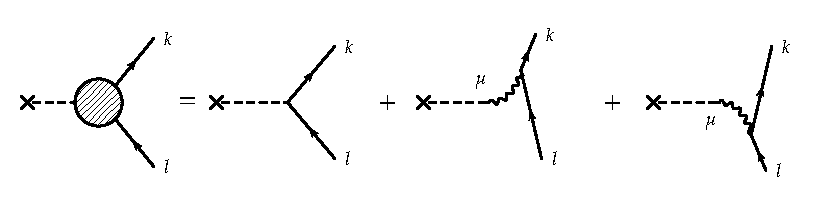
\includegraphics[width=0.7\textwidth]{pictures/9_9}
\par\end{centering}
\caption{\label{fig:9.9}有效电荷的费曼图图形表示。外场激发了核芯的虚振动声子，进而与外加价核子发生相互作用。}
\end{figure}

由式 (\ref{eq:9.156}) 可以看出，粒子-振动耦合将裸矩阵元 $T_{kl}$ 重整化为有效矩阵元 $T^{\text{eff}}_{kl}$。其微观物理根源在于：外场可以激发偶核核芯的虚振动（声子激发），并通过核力与外部价核子发生强烈的动力学相互作用。若该振动模式具有高度的集体性，它将使得矩阵元数值发生极为显著的改变。有效矩阵元的微观机制在\ref{fig:9.9}中给出了直观的费曼图表示。

体现这一动力学过程重要性的典型范例是闭壳核邻近单粒子态的有效电荷。在 2.7.2 节中我们已经看到，为了复现实验测得的质子与中子电多极矩和跃迁几率，必须引入有效电荷（通常取
$e^{\text{eff}}_{\text{p}}\approx2$，$e^{\text{eff}}_{\text{n}}\approx1$）。其物理原因正是\ref{fig:9.9}所示的核芯虚声子激发极化效应。我们的有效矩阵元式
(\ref{eq:9.156}) 可以进一步改写为：
\begin{equation}
T^{\text{eff}}_{kl}=T_{kl}+\sum_{mn}e^{\text{pol}}_{klmn}T_{mn},\label{eq:9.157}
\end{equation}
其中极化电荷 $e^{\text{pol}}=e^{\text{pol}}(\epsilon_{k}-\epsilon_{l})$
此时是一个依赖于单粒子能量差 $\epsilon_{k}-\epsilon_{l}$ 的动力学算符。将这一动力学算符用一个常数替代，便对应于唯象的有效电荷概念：
\begin{equation}
e^{\text{eff}}=1+e^{\text{pol}}.\label{eq:9.158}
\end{equation}
例如，在计算四极矩的有效电荷时，我们必须对偶核核芯的所有集体 $2^{+}$ 态的贡献进行求和。特别地，这意味着必须将巨四极共振（GQR，参见第
8 章）的激发全面计入。这类微观计算已在例如 Pb 同位素区开展 \cite{RBS73}，所得理论预言与实验结果高度符合。

有效矩阵元的定量计算需要预先求解 RPA 振幅 $X^{\mu}_{mi}$、$Y^{\mu}_{mi}$ 及其本征能量 $\Omega_{\mu}$。利用
RPA 方程（式 8.131），我们可以直接推导出关于 $T^{\text{eff}}$ 的闭合积分方程（亦可参见 Migdal
的工作 \cite{Mi67}）：
\begin{equation}
T^{\text{eff}}_{kl}(\omega)=T_{kl}+\sum_{pq}\bar{v}_{kqlp}\frac{n_{q}-n_{p}}{\omega-\epsilon_{p}+\epsilon_{q}}T^{\text{eff}}_{pq}(\omega).\label{eq:9.159}
\end{equation}
该方程直观地揭示了介质中的粒子-空穴极化传播子如何将外场有效驱动力重整化。

\section{\label{sec:9.3.6}\label{subsec:9.3.6_=004E2D=007B49=008026=005408=004E0EDyson=0073BB=008272=005C55=005F00}中间耦合与
Dyson 玻色展开}

前述各节中所阐述的粒子-振动耦合微扰处理方案，显然只有在极端弱耦合极限下才是严格有效的；在该极限下，$H_{\text{coupl}}$
的非对角矩阵元相比于对角能量项必须极其微小。然而事实表明，即便在被视作弱耦合原型的典型范例——$^{209}\text{Bi}$
的七重态（septuplet，详见下文讨论）中，这一条件也未能完全得到满足。为了克服微扰论的局限性，我们固然可以在未微扰基底（$H_{\text{coupl}}=0$）中对全
Hamiltonian 式 (\ref{eq:9.130}) 与式 (\ref{eq:9.131}) 进行严格对角化，但与此同时，我们必须将
Hamiltonian 的玻色展开式 (\ref{eq:9.131}) 推进到更高阶次，以确保达到所谓的水平收敛（horizontal
convergence，参见\ref{fig:9.3}）。然而迄今为止，这一完整方案在实践中极少被完全实现，主要应用于奇核系统的实际理论往往是另一类玻色理论——核场论（Nuclear
Field Theory, NFT；例如参见 \cite{Re75b,BBB77} 及其所引文献）。NFT 是一种高度非线性的代数理论，但已有严格证明表明
\cite{IRS79}，存在一种精巧的数学对应关系，可将非线性的 NFT 精确归结为线性的 Dyson 玻色展开（DBE），而
DBE 理论本身也已被成功应用于处理许多真实的复杂原子核系统 \cite{DJ73,RS74b,SWR76,IRS80}。鉴于线性代数方程在计算与概念处理上通常远比非线性理论简便，我们在本节中将专门阐述
DBE 方法。这使得我们能够大范围沿用在偶核系统中所建立的形式体系。正如偶核情形一样，奇核系统的 DBE 展开同样具有严格截断的有限阶代数结构。

对于集体玻色子，费米子对算符在奇核系统中的 DBE 映射形式为（非集体版本可参见 \cite{DJ73}）：
\begin{align}
(b^{\dagger}_{\mu})_{B} & =B^{\dagger}_{\mu}-\frac{1}{2}\sum_{\nu\rho\sigma}\Gamma^{\nu\rho}_{\mu\sigma}B^{\dagger}_{\nu}B^{\dagger}_{\rho}B_{\sigma}-\sum_{kl\nu}\Gamma^{\nu k}_{\mu l}B^{\dagger}_{\nu}\beta^{\dagger}_{k}\beta_{l},\nonumber \\
(b_{\mu})_{B} & =B_{\mu},\label{eq:9.160}\\
(a_{\mu\nu})_{B} & =\sum_{\rho\sigma}\Gamma^{\mu\rho}_{\nu\sigma}B^{\dagger}_{\rho}B_{\sigma}+\sum_{kl}\Gamma^{\mu k}_{\nu l}\beta^{\dagger}_{k}\beta_{l}.\nonumber 
\end{align}
将这些代数映射代入准粒子 Hamiltonian 式 (\ref{eq:9.32}) 中，并在如下由单准粒子与单声子构成的截断基底空间中进行对角化：
\begin{equation}
|A+1,\nu)=\sum_{p}C^{(\nu)}_{p}\beta^{\dagger}_{p}|0)+\sum_{p\mu}C^{(\nu)}_{p\mu}\beta^{\dagger}_{p}B^{\dagger}_{\mu}|0),\label{eq:9.161}
\end{equation}
即可直接导出如下久期矩阵方程：
\begin{equation}
\sum_{p'\mu'}\begin{pmatrix}\delta_{pp'}E_{p} & \frac{1}{2}\gamma^{\mu'*}_{p'p}\\
\frac{1}{2}\gamma^{\mu}_{pp'} & (\Omega_{\mu}+E_{p})\delta_{pp'}\delta_{\mu\mu'}+B_{p\mu p'\mu'}
\end{pmatrix}\begin{pmatrix}C^{(\nu)}_{p'}\\
C^{(\nu)}_{p'\mu'}
\end{pmatrix}=\omega^{(\nu)}\begin{pmatrix}C^{(\nu)}_{p}\\
C^{(\nu)}_{p\mu}
\end{pmatrix},\label{eq:9.162}
\end{equation}
其中 $\gamma^{\mu}_{p'p}$ 定义于式 (\ref{eq:9.132})，而诱导对角修正矩阵 $B$ 具有显式结构：
\begin{equation}
B_{p\mu p'\mu'}=-\sum_{l}(\Omega_{\mu'}-E_{l}-E_{p})C^{\mu}_{p'l}C^{\mu'*}_{pl}.\label{eq:9.163}
\end{equation}
在建立式 (\ref{eq:9.162}) 时，我们利用了准粒子 TDA 方程 {[}式 (8.10) 与式 (9.70){]}。矩阵元
(\ref{eq:9.162}) 的求值十分直接，仅有对 $H^{11}$ {[}见式 (9.32){]} 的处理较为繁琐。在无配对关联的极限下，对
$\mu'$ 的求和自然同时涵盖了 $ph$ 与 $pp$ 振动模式。这一代数对应关系可借助式 (9.133)、(8.201)
与 (8.202) 轻松推导。显而易见，与偶核情形完全相同，式 (\ref{eq:9.162}) 中的本征矩阵是非厄米的。

为了深入剖析修正矩阵 $B$ 的微观物理涵义，我们转到无超流关联的 HF 极限，在此极限下可以明确区分 $ph$ 与 $pp$
振动激发。此时我们清晰地看到，矩阵 $B$ 不仅能够耦合 $p\text{-}ph$ 与 $h\text{-}pp$ 组态，还同时在
$p\text{-}ph$ 组态彼此之间产生耦合。对照\ref{fig:9.8}(c) 所示的自能交换图，后一种耦合精确执行了对
Pauli 原理的动力学修正。由于显而易见的原因，$h\text{-}pp$ 与 $h\text{-}pp$ 组态之间不存在 Pauli
原理的重叠干涉，因此相应的矩阵元 $B_{h\text{-}pp,h\text{-}pp}$ 自然恒等于零。展开系数 $C^{(\nu)}_{p\mu}$
的物理涵义非常明确：它作为谱因子（spectroscopic factor），刻画了集体激发态在多大程度上由奇核准粒子的非关联运动与偶核核芯的集体声子振动耦合而成。这里的准粒子既可以是价粒子，也可以是空穴。例如，$^{209}\text{Bi}$
七重态的本征系数 $C^{(\nu)}_{p\mu}$ 直观揭示了该态究竟有多少成分是由单粒子与 $^{208}\text{Pb}$
的 $ph$ 振动耦合而成，又有多少成分是由空穴与 $^{210}\text{Pb}$、$^{210}\text{Po}$ 及
$^{210}\text{Bi}$ 的 $pp$ 振动耦合而成。必须指出的是，式 (\ref{eq:9.162}) 对应于一个非正交基底空间，因此这些系数仅代表相对几率幅。

矩阵方程 (\ref{eq:9.162}) 的代数维度显然远大于原始费米子物理空间的维度；但由于玻色子具有极强的集体性，我们完全有理由对基底空间进行大幅度截断。由于基底的过完备性，式
(\ref{eq:9.162}) 的解集不可避免地混杂着非物理的赝态（spurious solutions）。然而与偶核情形完全类似
{[}参见式 (9.98){]}，这些赝态全部落在自由三准粒子未微扰能量的极高位置处，因而远高于我们所关心的低能集体振动能级。因此，对于基底截断已经实现垂直收敛（vertical
convergence，见\ref{fig:9.3}）的系统，赝态绝不会造成任何实际困扰。在此情形下，所有感兴趣的低能本征值均为严格实数，矩阵的非厄米性亦不构成障碍。而对于核芯集体性并不十分显著、赝态与物理态可能相互交织的情形，一种极佳的处方是对范数度规矩阵进行对角化，通过剔除其零本征值（或实际计算中小于某一阈值
$\epsilon$ 的小本征值），将方程 (\ref{eq:9.162}) 严格变换为一个正交归一的厄米本征问题 \cite{IRS80,BSL79}。通过对剩余的对角范数矩阵求平方根并求逆，即可完成基底的正交归一化。该过程的具体数学细节将在
10.2 节中深入阐述。厄米化后的问题维度绝不会超过原始费米子空间的真实维度，从而彻底在数学上排除了任何赝态的侵入。正交归一化基底在精确计算电磁跃迁几率时亦展现出突出的代数优势。

为了深入领会上述物理与代数机制，考察一个虽然带有学术假定但完全可严格解析求解的三粒子模型是极具启发性的：在忽略配对关联且在闭壳核外存在三个价核子的情形下，式
(\ref{eq:9.162}) 中的粒子-振动耦合顶点 $\gamma$ 严格为零，我们得到如下简化的本征矩阵方程（其中 $p,m,n$
代表单粒子态，$\tau,\tau'$ 代表 $pp$ 振动模式）：
\begin{equation}
\sum_{\tau'p'}B_{p\tau p'\tau'}C^{(\nu)}_{p'\tau'}=\left(\omega^{(\nu)}-\Omega_{\tau}-\epsilon_{p}\right)C^{(\nu)}_{p\tau},\label{eq:9.164}
\end{equation}
其中相互作用核为：
\begin{equation}
B_{p\tau p'\tau'}=\sum_{n}C^{\tau*}_{p'n}(\Omega_{\tau'}-\epsilon_{n}-\epsilon_{p})C^{\tau'}_{np},\label{eq:9.165}
\end{equation}
这里的 $C^{\tau}_{mn}$ 与 $\Omega_{\tau}$ 是标准 $pp$-TDA 方程的本征解。

\begin{figure}[H]
\begin{centering}
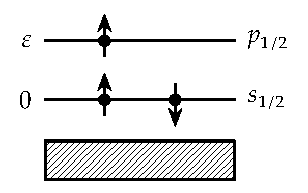
\includegraphics[width=0.4\textwidth]{pictures/9_10}
\par\end{centering}
\caption{\label{fig:9.10}解析可解模型的三个价核子能级组态示意图。}
\end{figure}

作为具体模型，我们考虑处于 $s_{1/2}$ 与 $p_{1/2}$ 能级中的三个价核子系统（如\ref{fig:9.10}所示）。在全部组态中，具有负宇称且自旋向上的物理纯费米子态仅有一个：
\[
|\alpha\rangle=a^{\dagger}_{s\frac{1}{2}}a^{\dagger}_{s-\frac{1}{2}}a^{\dagger}_{p\frac{1}{2}}|D\rangle.
\]
该纯物理态相对于核芯 $|D\rangle$ 的能量期望值可以直接计算求得：
\begin{align*}
\langle\alpha|H|\alpha\rangle-\langle D|H|D\rangle & =\epsilon+v_{s\frac{1}{2}s-\frac{1}{2},s\frac{1}{2}s-\frac{1}{2}}+v_{s\frac{1}{2}p\frac{1}{2},s\frac{1}{2}p\frac{1}{2}}+v_{s-\frac{1}{2}p\frac{1}{2},s-\frac{1}{2}p\frac{1}{2}}\\
 & =\epsilon+G+F+H.
\end{align*}
接下来我们需要计算两体激发态；假定双粒子剩余相互作用仅有对角矩阵元非零，我们可解出如下五个相关的两体 $\tau$ 模式：
\begin{align*}
C^{\tau_{1}}_{s\frac{1}{2}p\frac{1}{2}} & =1,\quad\Omega_{\tau_{1}}=\epsilon+F;\\
C^{\tau_{2}}_{s-\frac{1}{2}p\frac{1}{2}} & =1,\quad\Omega_{\tau_{2}}=\epsilon+H;\\
C^{\tau_{3}}_{s\frac{1}{2}s-\frac{1}{2}} & =1,\quad\Omega_{\tau_{3}}=G;\\
C^{\tau_{4}}_{s\frac{1}{2}p-\frac{1}{2}} & =1,\quad\Omega_{\tau_{4}}=\epsilon+v_{s\frac{1}{2}p-\frac{1}{2},s\frac{1}{2}p-\frac{1}{2}}:=\epsilon+I;\\
C^{\tau_{5}}_{p\frac{1}{2}p-\frac{1}{2}} & =1,\quad\Omega_{\tau_{5}}=2\epsilon+v_{p\frac{1}{2}p-\frac{1}{2},p\frac{1}{2}p-\frac{1}{2}}:=2\epsilon+J.
\end{align*}
对应的五种粒子-玻色子 $p\tau$ 组态展示于\ref{fig:9.11}中。

\begin{figure}[H]
\begin{centering}
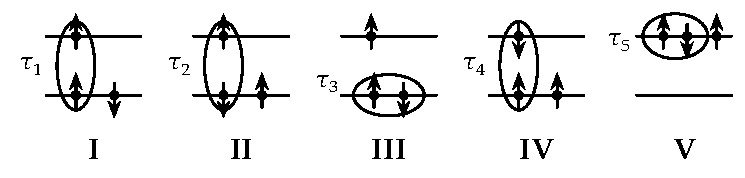
\includegraphics[width=0.7\textwidth]{pictures/9_11}
\par\end{centering}
\caption{\label{fig:9.11}三粒子模型中的五种可能的粒子-玻色子组态示意图（标号分别为 I、II、III、IV、V）。}
\end{figure}

由\ref{fig:9.11}可以极其清晰地看到：由于在构造基底态时忽略了 Pauli 原理，基底维度从物理上的 1 维急剧膨胀为
5 维，即此时的玻色空间是严重过完备的。现在我们来具体计算式 (\ref{eq:9.165}) 的相互作用矩阵（将不同的 $p\tau$
组态简记为 I、II、III、IV、V）：
\begin{align*}
B_{\text{I I}} & =\sum_{n}C^{\tau_{1}}_{s-\frac{1}{2}n}(\epsilon+F-\epsilon_{n}-0)C^{\tau_{1}}_{ns-\frac{1}{2}}=0,\\
B_{\text{I II}} & =\sum_{n}C^{\tau_{1}}_{s-\frac{1}{2}n}(\epsilon+H-\epsilon_{n}-0)C^{\tau_{2}}_{ns-\frac{1}{2}}=-H,\\
B_{\text{I III}} & =-G,\\
B_{\text{I IV}} & =B_{\text{I V}}=0.
\end{align*}
对全矩阵的全部元素依此类推，我们最终得到本征方程 (\ref{eq:9.164}) 的如下久期行列式：
\[
\begin{vmatrix}\epsilon+F-\omega^{(\alpha)} & -H & -G & 0 & 0\\
-F & \epsilon+H-\omega^{(\alpha)} & G & 0 & 0\\
-F & H & \epsilon+G-\omega^{(\alpha)} & 0 & 0\\
0 & 0 & 0 & \epsilon-\omega^{(\alpha)} & 0\\
0 & 0 & 0 & 0 & 2\epsilon-\omega^{(\alpha)}
\end{vmatrix}=0.
\]
显而易见，该矩阵是非厄米的。直接求出行列式的特征多项式根，可得到其全部本征值为：
\[
\omega^{(1)}=\omega^{(2)}=\omega^{(3)}=\epsilon;\quad\omega^{(4)}=2\epsilon;\quad\omega^{(5)}=\epsilon+F+G+H.
\]
我们由此惊奇而漂亮地发现：本征谱精确地重现了真物理态的能量 $\epsilon+F+G+H$，而伴随产生的四个多余本征态全部是不具相互作用的未微扰纯单粒子（或空穴）能量！这与我们在偶核
DBE 理论中推得的结论完全契合：过完备基底引入的全部非物理赝态严格定域于未微扰单粒子能量处。尽管本模型具有教学演示的理想简化性质，但在偶核核芯存在极强集体激发态的实际原子核中，通过截断后所需对角化的有效玻色矩阵规模将远远小于全费米子多体组态空间。

\begin{figure}[H]
\begin{centering}
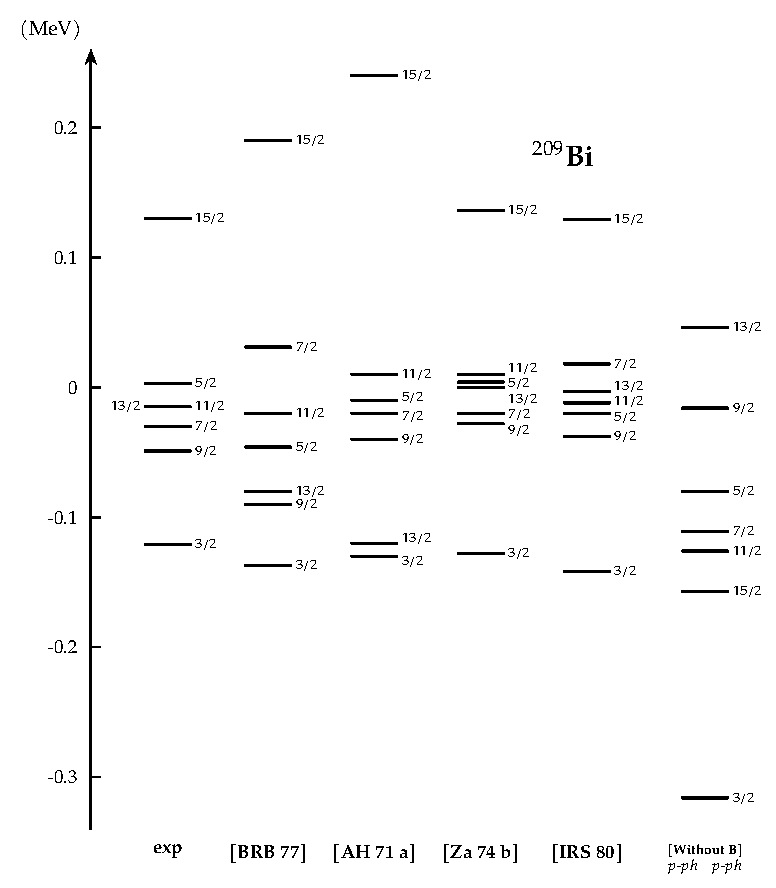
\includegraphics[width=0.75\textwidth]{pictures/9_12}
\par\end{centering}
\caption{\label{fig:9.12}$^{209}\text{Bi}$ 中粒子-振动耦合态（七重态）的能谱：展示了实验测量能级以及不同理论作者给出的计算结果。在最后一列中，人为略去了式
(9.162) 中的 $B_{p\text{-}ph,p\text{-}ph}$ 矩阵元，以直观彰显 Pauli 原理的剧烈重整化效应。零能量基准线取为
$^{208}\text{Pb}$ 中 $3^{-}$ 态的激发能（2.614 MeV）。}
\end{figure}

作为具体物理应用，\ref{fig:9.12}展示了利用 DBE 求解式 (\ref{eq:9.162}) 并逐步扩展基底维度直至垂直收敛所计算的
$^{209}\text{Bi}$ 七重态（septuplet）能谱。图中同时列出了利用核场论（NFT）\cite{BBB77}
以及其他学者采用不同微观方法 \cite{AH71a,Za74b} 所得的理论结果与实验数据的系统比对。在\ref{tab:9.2}中，我们给出了若干主要波函数分量
$C^{(\nu)}_{p\mu}$（谱因子），以清晰展示其相对重要性。\ref{fig:9.12}无可辩驳地证明了严谨计入 Pauli
原理修正的关键性：若人为关闭式 (\ref{eq:9.162}) 中的 $B_{p\text{-}ph,p\text{-}ph}$
矩阵元（即图中最右侧一列），计算出的能级裂距将产生完全背离实验的严重畸变。理论与实验之间尚存的微小偏差主要归因于两点：第一，$2p\text{-}1h$
组态是构筑七重态的主导成分，计算中处理了其与 $1p$ 空间的弱耦合，但忽略了与 $3p\text{-}2h$ 复杂组态的耦合；出于对称性考虑，高阶组态理应被完整计入，然而这在数值计算实践中极其繁复；第二，基底截断和相互作用参数的选取仍存在微小唯象调整空间。

\begin{table}[H]
\caption{\label{tab:9.2}$^{209}\text{Bi}$ 七重态中若干粒子-振动耦合态的波函数结构（以谱因子 $C_{p\mu}$
给出）。主导成分 $\pi h_{9/2}\otimes{}^{208}\text{Pb}(3^{-})$ 归一化为 1.0（引自
\cite{IRS80}）。}

\centering{}%
\begin{tabular}{lccc}
\toprule 
$p\quad\mu$ & $3/2$ & $5/2$ & $7/2$\tabularnewline
\midrule
纯单粒子态 & 0.005 & 0.001 & 0.026\tabularnewline
$\pi h_{9/2}\otimes{}^{208}\text{Pb}(3^{-})$ & 1.0 & 1.0 & 1.0\tabularnewline
$\pi h_{9/2}\otimes{}^{208}\text{Pb}(6^{+}_{1})$ & $-0.385$ & 0.266 & $-0.233$\tabularnewline
$\nu g_{9/2}\otimes{}^{208}\text{Bi}(6^{+}_{2})$ & $-0.406$ & 0.356 & $-0.320$\tabularnewline
$\nu i_{11/2}\otimes{}^{208}\text{Bi}(6^{+}_{1})$ & 0.100 & $-0.155$ & 0.211\tabularnewline
$\nu i_{11/2}\otimes{}^{208}\text{Bi}(7^{+}_{1})$ & $-0.318$ & 0.282 & $-0.232$\tabularnewline
$(\pi d_{3/2})^{-1}\otimes{}^{210}\text{Po}(0^{+})$ & 0.326 & — & —\tabularnewline
$(\pi d_{3/2})^{-1}\otimes{}^{210}\text{Po}(2^{+})$ & 0.233 & 0.231 & 0.095\tabularnewline
$(\pi d_{3/2})^{-1}\otimes{}^{210}\text{Po}(4^{+})$ & — & 0.200 & 0.282\tabularnewline
$(\nu p_{3/2})^{-1}\otimes{}^{210}\text{Bi}(1^{-})$ & 0.286 & $-0.128$ & —\tabularnewline
$(\nu p_{3/2})^{-1}\otimes{}^{210}\text{Bi}(2^{-})$ & 0.225 & 0.205 & 0.090\tabularnewline
$(\nu p_{3/2})^{-1}\otimes{}^{210}\text{Bi}(3^{-})$ & 0.151 & 0.234 & 0.191\tabularnewline
$(\nu p_{3/2})^{-1}\otimes{}^{210}\text{Bi}(4^{-})$ & — & $-0.181$ & $-0.255$\tabularnewline
$(\nu p_{3/2})^{-1}\otimes{}^{210}\text{Bi}(5^{-})$ & — & — & $-0.235$\tabularnewline
\bottomrule
\end{tabular}
\end{table}


\section{\label{sec:9.3.7}其它粒子-振动耦合计算}

正如我们在本节伊始所指出的，在核物理中存在许多不同类型的弱耦合理论应用，我们在此无法一一详尽展开。例如，对于必须计入超流对关联的球形开壳核系统，我们尚未讨论各类准粒子-声子耦合理论
\cite{KS63,DJ73}。在这一方向上最为精深且先进的微观理论之一——虽然其庞大的代数体系已经超出了本书的范围——是由 Marumori
及其合作者所创立的理论体系 \cite{KMM72,KMM75a,KMM75b}。

\begin{figure}[H]
\begin{centering}
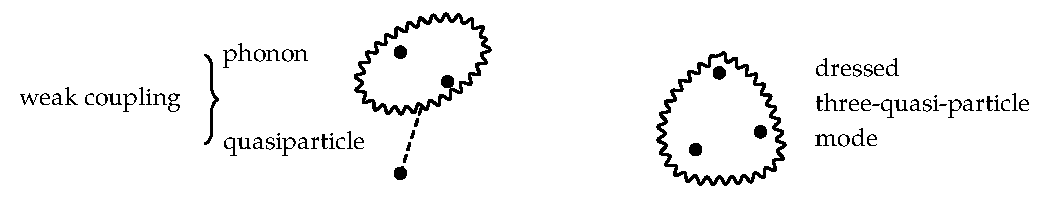
\includegraphics[width=0.7\textwidth]{pictures/9_13}
\par\end{centering}
\caption{\label{fig:9.13}准粒子-声子（弱耦合）与缀饰三准粒子模式（强耦合）的示意图表示。}
\end{figure}

该理论不仅能够描述弱耦合情形，而且能够极其精确地刻画三个准粒子发生强烈纠缠与多体重整化的强耦合情形（缀饰三准粒子模式，dressed
three-quasiparticle mode，见\ref{fig:9.13}；当然 DBE 同样具备这种能力）；更重要的是，它系统计入了基态关联（ground
state correlations），并且严格排除了由于 BCS 理论破坏粒子数守恒所引入的非物理赝成分。

\begin{figure}[H]
\begin{centering}
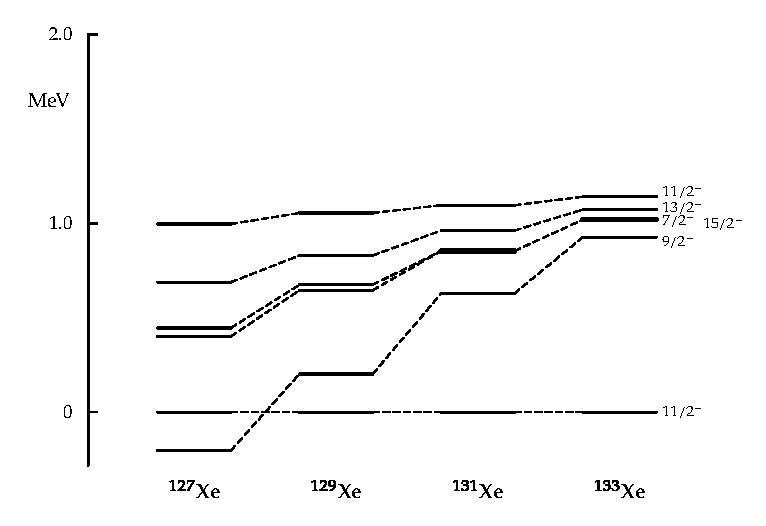
\includegraphics[width=0.7\textwidth]{pictures/9_14}
\par\end{centering}
\caption{\label{fig:9.14}一系列 Xe 同位素中粒子-振动耦合态的能量系统学演化（引自 \cite{KMM75a}）。}
\end{figure}

展现该理论威力的一个极佳应用范例，是一系列 Xe 与 Te 同位素中奇中子 $h_{11/2}$ 态与核芯 $2^{+}$ 声子态的耦合问题，其展现了从弱耦合向强耦合平滑过渡的清晰物理图像（见\ref{fig:9.14}）。在
Xe 同位素链中，从 $^{133}\text{Xe}$ 走向 $^{127}\text{Xe}$——亦即朝向 $h_{11/2}$
壳层中央演化时，我们观察到多重态的能级劈裂急剧增大；对于 $^{127}\text{Xe}$，能级劈裂已经如此剧烈，以至于多重态中能量最低的分支——即
$9/2^{-}$ 态（强烈关联的缀饰三准粒子态）——其能量甚至反常地低于奇中子本身的未微扰单粒子 $11/2^{-}$ 态！这类能级在核物理中通常被称为“反常耦合态”（abnormal
coupling states）。其物理起源归结为两种协同效应：
\begin{enumerate}
\item 几何代数效应：在单粒子角动量 $j$ 与 $2^{+}$ 声子的角动量耦合中，$j-1$ 态在几何对称性上始终是该多重态中能量最低的成员（参见
\cite{KMM75a}）；
\item 动力学关联效应：随着原子核越来越接近壳层中部，基态（BCS）配对关联急剧增强。可以严格证明，此时\ref{fig:9.8}(c)
所代表的对易自能修正图变得极其巨大且占据主导地位。
\end{enumerate}
在 Te 同位素链中，这种耦合强度相对较弱，因而在实验上并未发生反常耦合反转现象。理论所给出的能级系统学演化趋势与实验测量得到了非常完美的符合。

\section{\label{sec:9.3.8}偶偶系统中的弱耦合}

在原子核理论中，还广泛存在着许多其他类型的弱耦合物理图像。弱耦合决非仅仅局限于奇 $A$ 核系统——在偶偶核中同样存在显著的弱耦合现象。例如，$^{208}\text{Pb}$
中的双 $3^{-}$ 声子四重态（$3^{-}\otimes3^{-}\to0^{+},2^{+},4^{+},6^{+}$；迄今实验上仅确证了
$0^{+}$ 与 $2^{+}$ 两个能级）极有可能属于典型的弱耦合类型 \cite{BBN74a,Sch76}。从理论观点来看，最好能采用一种能够同时统一描述弱耦合、中间耦合乃至强耦合情境的理论形式体系；正如前文所展示的，对于双幻核或邻近幻核的体系，Dyson
玻色展开（DBE）正是这样一种理想的微观形式体系。

在处理单声子与双声子态的动力学耦合时，偶核系统的波函数可表达为如下形式：
\begin{equation}
|\tilde{\nu})=\sum_{\mu}C^{(\nu)}_{\mu}\tilde{B}^{\dagger}_{\mu}|0)+\sum_{\mu_{1}\mu_{2}}C^{(\nu)}_{\mu_{1}\mu_{2}}\tilde{B}^{\dagger}_{\mu_{1}}\tilde{B}^{\dagger}_{\mu_{2}}|0),\label{eq:9.166}
\end{equation}
其中指标 $\mu$ 的求和自然同时包括 $ph$ 与 $pp$ 振动模式。相应的 DBE 矩阵具有如下结构：
\begin{equation}
\begin{pmatrix}\Omega_{\mu}\delta_{\mu\mu'} & -\frac{1}{2}\sum_{kl}\gamma^{\mu_{1}'}_{kl}\Gamma^{\mu_{2}'k}_{\mu'l}-(\mu_{1}'\leftrightarrow\mu_{2}')\\
-\frac{1}{2}\sum_{kl}\gamma^{\mu_{1}}_{kl}\Gamma^{\mu_{2}k}_{\mu'l}-(\mu_{1}\leftrightarrow\mu_{2}) & (\Omega_{\mu_{1}}+\Omega_{\mu_{2}})\delta_{\mu_{1}\mu_{1}'}\delta_{\mu_{2}\mu_{2}'}+W_{\mu_{1}\mu_{2}\mu_{1}'\mu_{2}'}
\end{pmatrix},\label{eq:9.167}
\end{equation}
其中顶点 $\gamma^{\mu}_{kl}$ 见式 (\ref{eq:9.132})，结构常数 $\Gamma^{\nu k}_{\mu l}$
见式 (\ref{eq:9.29})，而四声子相互作用矩阵元 $W_{\mu_{1}\mu_{2}\mu_{1}'\mu_{2}'}$
定义于式 (\ref{eq:9.72})。该矩阵方程已被用于数值求解 $^{208}\text{Pb}$ 中的 $3^{-}\otimes3^{-}$
四重态 \cite{Sch76}。计算表明，仅需包含大约 10–20 个组态即可在垂直方向上迅速实现数值收敛（见\ref{fig:9.3}），所求得的四重态能级劈裂仅在
100 keV 左右，这定量证实了该态高度接近弱耦合图景。

对于超流核系统，由于粒子数守恒的破缺，必须建立更为精细的完备理论。这一工作已由 Marumori 研究组彻底完成 \cite{IMS76}。利用这种理论，物理学家成功解释了某些
Ge 同位素中第二个 $0^{+}$ 态能量异常低沉的物理之谜：它被证实是由对振动（pairing vibration）与 $(2^{+}\otimes2^{+})$
四重态中的 $0^{+}$ 成员之间极强的非谐相互干涉所引发的。Ge 同位素对对振动表现得如此“软”（soft），其深层原因可以从单粒子能级密度中得到理解：在这些核中，Fermi
面下方的能级密度极低（仅有 $j=1/2$ 态），而在 Fermi 面的正上方紧邻着极高的单粒子能级密度（$j=9/2$ 态）。正如我们在第
6 章和第 7 章中所深入讨论的，高能级密度极其有利于对关联的发展，核子因此具有强烈的动力学倾向去充分占据 Fermi 面上方宽广的相空间。这使得这些核在对激发模式上表现出高度非线性的强非谐性。

上述物理讨论总结了我们对原子核中非谐效应的全面研究。在这一研究进程中我们清晰地看到，玻色描述方法对于刻画偶核与奇核系统的集体与非谐现象都是极为有力和适用的。然而，为了在实际数值应用的各个层面全面确立和检验该微观方法的优越性，仍需在未来开展更加广泛深入的数值计算与实验检验。



\chapter{生成坐标法\label{chap:=00751F=006210=005750=006807=006CD5}}

\section{引言}

迄今为止，对集体运动的微观描述都是建立在选取尽可能多包含关联的广义直积态的基础之上的。以此图像为出发点，通过引入类玻色子激发进一步考虑了更多的关联。原则上，在玻色子图像中能够获得精确的本征态，但在实际计算中我们必须受限于有限数目的玻色子。其结果是，我们能够很好地描述在形变方面较为“刚性”的原子核中的简谐振动，以及过渡区核中的非简谐效应。然而，对于那些极其软、几乎处于塌缩边缘的原子核（即处于相变附近），有限阶的玻色展开技术可能不再足够。我们至少必须进行直至无穷阶的部分求和。显而易见，例如在涉及真正大振幅集体运动（large
amplitude collective motions, LACM）的核裂变过程中，正是这种必须超越迄今所考虑理论的新框架的候选对象。为了处理这些情况，物理学界实质上提出了两种主要理论：生成坐标法（Generator
Coordinate Method, GCM）与时间相关 Hartree-Fock 理论（Time-Dependent Hartree-Fock,
TDHF）。在本章中，我们将讨论 GCM。它是一种完全微观的量子力学方法，通过构建许多不同直积波函数的线性叠加而形成；在某种意义上，它是分子物理学中原子轨道线性组合（linear
combination of atomic orbital, LCAO）方法推广到具有连续标记基函数情形时的对应理论 \cite{MEL76}。该方法可用于处理诸多不同问题，例如多体理论中对称性的恰当处理（投影方法，第
11 章）、轻核散射（共振群方法，resonating group method \cite{HW53,Bi77}），以及核结构中大振幅集体激发（裂变、巨共振、形状与对振动）。

在第 10.2 节中，我们将介绍 GCM 的基本概念，并在第 10.3 节将其应用于 Lipkin 模型。GCM 与玻色展开之间的密切关系将在第
10.4 节中讨论。简谐振子是一个极具启发性的示例（第 10.5 节）。复生成坐标将在第 10.6 节中讨论。将 GCM 应用于集体运动理论的重要原因之一在于，我们能够以完全微观量子力学的方式导出一个集体
Hamiltonian，从而为第 1 章介绍的唯象集体模型建立微观联系（第 10.7 节）。在第 10.8 节中，我们将介绍一种能够确定最优生成函数的方法。GCM
的若干具体物理应用将在第 10.9 节中进行讨论。

\section{基本概念}

\subsection{波函数的 GCM 拟设}

生成坐标法由对试探波函数的一个极其普适的拟设构成。它是所谓的``生成函数（generating functions）''$|\Phi(a)\rangle$的连续叠加，这些生成函数由无限多个实参数或复参数$\{a\}=a_{1},a_{2},\dots,a_{n}$（即所谓的``生成坐标''，generator
coordinates）所标记；正如多体 Hilbert 空间中的真实波函数一样，它们也依赖于微观核子的坐标：

\begin{equation}
|\Psi\rangle=\int\mathrm{d}a\,f(a)|\Phi(a)\rangle.\label{eq:gcm_ansatz}
\end{equation}

该积分是一个多维积分，遍历参数$a$的所有实部和虚部。``生成坐标''这一名称在某种程度上带有误导性，因为在严格意义上，各个$a$并不是通常空间中的粒子力学坐标。GCM
并没有向多体系统引入任何多余的冗余坐标（redundant coordinates）。它们仅仅充当展开式\ref{eq:gcm_ansatz}中的一种连续求和指标。函数$f(a)$起着权重的作用，因而被称为``权重函数（weight
function）''，尽管正如我们将看到的，在严格的数学意义上它并不是系统的物理波函数。

生成函数集合$|\Phi(a)\rangle$——以及式\ref{eq:gcm_ansatz}中的积分限——可以按照我们的意愿任意选取。取决于函数$|\Phi(a)\rangle$的本质以及参数$a_{i}$的数目，拟设\ref{eq:gcm_ansatz}最终完全有可能包含
Schrödinger 方程的精确解。在很多实际情况下，我们采用直积波函数$|\Phi(a)\rangle$。一个典型的例子是具有形变参数$\beta$的势阱中的
Nilsson 波函数（见第 2 章）。在这一情形下，形变$\beta$即作为生成坐标。

另一个例子是最一般的 HFB 型直积波函数$|\Phi(z^{*})\rangle$\footnote{为方便起见，在此处我们采用$z^{*}$代替$z${[}参见式\ref{eq:coherent_state_gcm_ansatz}{]}。}，它们与某个基准态$|\Phi_{0}\rangle$不正交。根据
Thouless 定理（第 E.3 节），这类波函数由下式给出：

\begin{equation}
|\Phi(z^{*})\rangle=\mathscr{N}_{0}\exp\left(\frac{1}{2}\sum_{kk'}z_{kk'}\alpha^{\dagger}_{k}\alpha^{\dagger}_{k'}\right)|\Phi_{0}\rangle,\quad\langle\Phi_{0}|\Phi_{0}\rangle=1,\label{eq:thouless_theorem_generating_function}
\end{equation}

其中$z_{kk'}$（$k<k'$）为复数：

\begin{equation}
z_{kk'}=x_{kk'}+\mathrm{i}y_{kk'},\quad\int\mathrm{d}z=\int^{+\infty}_{-\infty}\prod_{k<k'}\mathrm{d}x_{kk'}\,\mathrm{d}y_{kk'}.\label{eq:complex_parameter_measure}
\end{equation}

在第 10.4 节中我们将看到，多体 Hamiltonian $H$ 的精确本征函数可以用式\ref{eq:thouless_theorem_generating_function}类型的生成函数精确表达。然而，在此情形下生成坐标$z_{kk'}$的数目极其巨大。对于实际的物理应用，我们必须尽可能减少它们的数目；这就需要深刻的物理直觉来选取一组生成函数$|\Phi(a)\rangle$，它既要足够普适以准确描述物理图景，又要足够简洁以便能够通过后续方法进行求解。因此一般而言，使用选定的一组生成函数，我们通过形如\ref{eq:gcm_ansatz}的拟设通常只能描述
Hamiltonian $H$ 的某特定类别的本征态。

\subsection{权重函数 f(a) 的确定}

假定拟设\ref{eq:gcm_ansatz}中的权重函数$f(a)$是变量$a$的良态函数（通常为平方可积函数），使得我们能够施行以下数学运算。为了确定函数$f(a)$，我们使用变分原理：

\begin{equation}
\delta\frac{\langle\Psi|H|\Psi\rangle}{\langle\Psi|\Psi\rangle}=0.\label{eq:gcm_variational_principle}
\end{equation}

对$f(a)$进行变分，可得积分方程：

\begin{equation}
\int\mathrm{d}a'\,\langle\Phi(a)|H|\Phi(a')\rangle f(a')=E\int\mathrm{d}a'\,\langle\Phi(a)|\Phi(a')\rangle f(a').\label{eq:hill_wheeler_equation}
\end{equation}

这一方程就是著名的 Hill-Wheeler 方程（HW 方程）\cite{HW53}。它可以形式地写为：

\begin{equation}
\mathscr{H}f=E\mathscr{N}f,\label{eq:hw_formal_matrix_equation}
\end{equation}

其中积分核为重叠函数（overlap functions）：

\begin{align}
\mathscr{H}(a,a') & =\langle\Phi(a)|H|\Phi(a')\rangle,\nonumber \\
\mathscr{N}(a,a') & =\langle\Phi(a)|\Phi(a')\rangle.\label{eq:overlap_functions_kernels}
\end{align}

在形式上，这与在非正交``基底''$|\Phi(a)\rangle$中对角化 Hamiltonian 非常相似 \cite{Wo70}。如果参数$a$（在下文中我们将主要限制在单个实参数的情形）仅取有限个离散值$a_{1},\dots,a_{M}$，则这显然是成立的。在那种情况下，存在有限个函数$|\Phi_{i}\rangle=|\Phi(a_{i})\rangle$，它们一般线性相关且并不完备。事实上，Hill-Wheeler
方程\ref{eq:hill_wheeler_equation}在数值上通常就是通过离散化来求解的。此时我们立即获得形如式\ref{eq:hw_formal_matrix_equation}的矩阵方程。然而，在连续参数$a$的一般情形下，正如我们将在下文所见，必须十分谨慎。

式\ref{eq:hw_formal_matrix_equation}的形式解是显而易见的：我们可以尝试对算符$\mathscr{N}$求逆，并对角化算符$\mathscr{N}^{-1}\mathscr{H}$。但这将给出一个非厄米本征值问题，且仅当算符$\mathscr{N}$完全没有零本征值时才可行。然而在实际中零本征值极其普遍，因为集合$|\Phi(a)\rangle$通常是线性相关的。因此，我们通过对集合$|\Phi(a)\rangle$进行正交化来解决这一问题。为此有数种可供选择的方法。最为人熟知的是
Gram-Schmidt 正交化步骤，它对应于将矩阵$\mathscr{N}$分解为两个三角矩阵（参见第 8.4.4 节）。另一种同样适用于连续变量情形的方法是对称正交化（symmetric
orthogonalization）。它对应于对角化厄米算符$\mathscr{N}$：

\begin{equation}
\int\mathrm{d}a'\,\mathscr{N}(a,a')u_{k}(a')=n_{k}u_{k}(a).\label{eq:norm_kernel_eigenvalue_problem}
\end{equation}

在下文中，我们假设本征谱$n_{k}$（$k=1,2,\dots$）是离散的\footnote{当$\mathscr{N}$属于 Hilbert-Schmidt 型（即厄米且具有有限迹$\mathrm{Tr}(\mathscr{N}^{\dagger}\mathscr{N})$\cite{RS72}）时确实如此。在许多实际情况下，积分核$\mathscr{N}$与$\mathscr{H}$并不满足此性质{[}例如式\ref{eq:ho_gaussian_generating_function}{]}。然而已有文献证明，通过适当改变参数化方式
\cite{TP78} 或通过给生成态乘以适当的重整化因子$r(a)$\cite{La76}，我们总能达成该性质。此外，在更弱的假定下该理论也可以大体相同的方式展开，此时存在连续谱（\cite{TP78}；并参见第
10.5 节）。}。由于$\mathscr{N}$是范数算符，其本征值恒非负（$n_{k}\ge0$）。

函数$u_{k}(a)$在权重函数$f(a)$的空间中构成一组完全标准正交基：

\begin{equation}
\sum_{k}u_{k}(a)u^{*}_{k}(a')=\delta(a-a');\quad\int\mathrm{d}a\,u^{*}_{k}(a)u_{k'}(a)=\delta_{kk'}.\label{eq:weight_basis_orthonormality}
\end{equation}

该空间中的算符$\mathscr{N}$可以分解为$\mathscr{N}=\mathscr{N}^{1/2}\cdot\mathscr{N}^{1/2}$，其中：

\begin{equation}
\mathscr{N}^{1/2}(a,a')=\sum_{k}u_{k}(a)\sqrt{n_{k}}\,u^{*}_{k}(a'),\label{eq:norm_operator_decomposition}
\end{equation}

从而我们可以在形式上推导出厄米本征值问题：

\begin{equation}
\mathscr{N}^{-1/2}\mathscr{H}\mathscr{N}^{-1/2}g=Eg,\label{eq:hermitian_g_eigenvalue_problem}
\end{equation}

其中：

\begin{equation}
f=\mathscr{N}^{-1/2}g.\label{eq:f_and_g_relation}
\end{equation}

若$\mathscr{N}$存在零本征值（$n_{k}=0$），则算符$\mathscr{N}^{1/2}$的求逆是不可能的。落在相应本征子空间中的权重函数$f^{0}(a)$所产生的多体波函数$|\Psi\rangle$恒等于零：

\begin{equation}
\langle\Psi|\Psi\rangle=\int\mathrm{d}a\,\mathrm{d}a'\,f^{0*}(a)\mathscr{N}(a,a')f^{0}(a')=0.\label{eq:zero_norm_many_body_norm}
\end{equation}

如果存在零本征值，则对应于 HW 态$|\Psi\rangle$的权重函数$f$不是唯一定义的。我们总能够给它加上任意一个函数$f^{0}$而获得完全相同的$|\Psi\rangle$。为了在$|\Psi\rangle$与权重函数$f$之间建立一一对应关系，我们至少应当将$f(a)$限制在那些由对应于$n_{k}\neq0$的函数$u_{k}(a)$线性组合而成的权重函数子空间中。对于这些函数中的每一个，在多体
Hilbert 空间中都存在一个归一化矢量：

\begin{equation}
|k\rangle=\frac{1}{\sqrt{n_{k}}}\int\mathrm{d}a\,u_{k}(a)|\Phi(a)\rangle.\label{eq:natural_states_definition}
\end{equation}

这些矢量被称为``自然态（natural states）''。极易证明它们相互正交。它们张成了一个子 Hilbert 空间$\mathfrak{H}_{C}$，即所谓的``集体子空间（collective
subspace）''。这是包含所有生成态$|\Phi(a)\rangle$的最小 Hilbert 空间。向该子空间的投影算符由下式给出：

\begin{equation}
P_{C}=\sum_{k,n_{k}\neq0}|k\rangle\langle k|.\label{eq:collective_subspace_projection}
\end{equation}

现在，我们不再求解式\ref{eq:hermitian_g_eigenvalue_problem}，而是在集体子空间内对角化有效算符$P_{C}HP_{C}$：

\begin{equation}
\sum_{k',n_{k'}\neq0}\langle k|H|k'\rangle g_{k'}=Eg_{k},\label{eq:collective_hamiltonian_diagonalization}
\end{equation}

其中矩阵元为：

\begin{equation}
(P_{C}HP_{C})_{kk'}=\langle k|H|k'\rangle=\frac{1}{\sqrt{n_{k}n_{k'}}}\int\mathrm{d}a\,\mathrm{d}a'\,u^{*}_{k}(a)\mathscr{H}(a,a')u_{k'}(a').\label{eq:collective_subspace_hamiltonian_matrix}
\end{equation}

本征态由下式给出：

\begin{equation}
|\Psi\rangle=\sum_{k,n_{k}\neq0}g_{k}|k\rangle.\label{eq:eigenstate_in_natural_basis}
\end{equation}

由式\ref{eq:natural_states_definition}，我们得到相应的权重函数：

\begin{equation}
f(a)=\sum_{k,n_{k}\neq0}\frac{g_{k}}{\sqrt{n_{k}}}u_{k}(a).\label{eq:weight_function_natural_expansion}
\end{equation}

如果非零本征值$n_{k}\neq0$只有有限个（或者更准确地说，如果零不是本征值序列$n_{k}$的极限点），则由式\ref{eq:weight_function_natural_expansion}定义的函数$f(a)$总是良定的。然而在连续参数的情形下，往往存在以零为极限点的无穷多个非零本征值$n_{k}$。从式\ref{eq:weight_function_natural_expansion}中容易看出，即使波函数$|\Psi\rangle$具有有限范数（$\sum|g_{k}|^{2}<\infty$），函数$f(a)$依然可能发生发散。这意味着在集体子空间$\mathfrak{H}_{C}$中存在着某些无法用具有良态数学性质函数$f(a)$的
Hill-Wheeler 态\ref{eq:gcm_ansatz}表示的矢量。此时对应的函数$f$具有广义函数（distributions）的性质{[}参见式\ref{eq:ho_weight_function_distribution_series}{]}。显而易见，我们绝不可能通过对积分进行单纯离散化来获得
Hill-Wheeler 方程\ref{eq:hill_wheeler_equation}的此类解\footnote{导致这些问题的深层数学根源在于：由具有良好数学性质的权重函数$f(a)$构成的 Hill-Wheeler 态\ref{eq:gcm_ansatz}所构成的线性空间，通常并不是一个
Hilbert 空间；因为它不具备完备闭合性，即对于每一个收敛的矢量序列$|\Psi_{i}\rangle$，并不必然存在一组收敛的良态权重函数序列$f_{i}(a)$。}。

粗略地说，GCM 拟设\ref{eq:gcm_ansatz}代表了多体波函数$|\Psi\rangle$关于非正交生成函数$|\Phi(a)\rangle$的展开。展开系数由权重函数$f(a)$给出。为了更好地理解该函数的物理意义，引入所谓的``双正交基（biorthogonal
basis）''是有益的 \cite{Wo70}。它由具有如下性质的态矢量$|\tilde{\Phi}(a)\rangle$给出：

\begin{equation}
\langle\tilde{\Phi}(a)|\Phi(a')\rangle=\delta(a-a').\label{eq:biorthogonal_basis_property}
\end{equation}

如果范数算符存在零本征值，我们显然只能要求：

\begin{equation}
\langle\tilde{\Phi}(a)|\Phi(a')\rangle=P_{\perp}(a,a')=\sum_{k,n_{k}\neq0}u_{k}(a)u^{*}_{k}(a'),\label{eq:biorthogonal_projection_property}
\end{equation}

其中$P_{\perp}$是向正交于式\ref{eq:norm_kernel_eigenvalue_problem}中具有本征值$n_{k}=0$的本征矢量$u_{k}(a)$的子空间上的投影算符。我们可以通过在自然态中展开来构造具有此性质的矢量$|\tilde{\Phi}\rangle$：

\begin{equation}
|\tilde{\Phi}(a)\rangle=\sum_{k,n_{k}\neq0}\frac{u^{*}_{k}(a)}{\sqrt{n_{k}}}|k\rangle.\label{eq:biorthogonal_states_natural_expansion}
\end{equation}

然而，如此定义的双正交态$|\tilde{\Phi}(a)\rangle$通常并不属于多体 Hilbert 空间，因为它们的范数并不必然有限。尽管如此，我们现在可以将对应于
Hill-Wheeler 态$|\Psi\rangle$的权重函数$f(a)$表征为：

\begin{equation}
f(a)=\langle\tilde{\Phi}(a)|\Psi\rangle.\label{eq:weight_function_biorthogonal_overlap}
\end{equation}

因此，$f(a)$度量的是波函数$|\Psi\rangle$与双正交基中的态矢量$|\tilde{\Phi}(a)\rangle$之间的重叠。它并不是在波函数$|\Psi\rangle$中找到生成态$|\Phi(a)\rangle$的几率振幅；后者是由$\langle\Phi(a)|\Psi\rangle$给出的。公式\ref{eq:weight_function_biorthogonal_overlap}再次阐明了$f(a)$并不必然是一个良态函数。

到目前为止，我们仅讨论了与 GCM 表象\ref{eq:gcm_ansatz}结构相关的问题。这些性质完全由该拟设所采用的生成函数集$|\Phi(a)\rangle$所决定。与第
9 章类似，我们称它们为``运动学性质（kinematic properties）''，因为它们仅与所采用的基础基底有关。我们尚未探究集合$|\Phi(a)\rangle$是否真正适合用于描述系统的
Hamiltonian 本征态，即$|\Psi\rangle$是否至少能在良好近似下表示为这些函数的线性叠加。换言之，我们尚未考察
GCM 拟设的动力学方面。

只有当 Hamiltonian 在良好近似下与集体投影算符$P_{C}$对易时：

\begin{equation}
[H,P_{C}]\simeq0,\label{eq:hamiltonian_collective_projection_commutation}
\end{equation}

我们才能指望从式\ref{eq:collective_hamiltonian_diagonalization}中求得接近系统精确波函数的多体态$|\Psi\rangle$。在此种情况下，集体子空间包含了$H$的本征态。该条件在多大程度上得到满足，完全取决于集合$|\Phi(a)\rangle$的物理选取。

\subsection{HW 方程的数值解法}

基于上述考虑，我们将极其简要地讨论求解 Hill-Wheeler 方程\ref{eq:hill_wheeler_equation}的数值方法。

（i）最直接的方法是对变量$a$的积分进行离散化。正如我们所看到的，在这种情况下我们最终面对一个矩阵方程。我们首先对角化范数矩阵，得到一组正交的本征矢量。在第二步中，我们限制在具有非零本征值——出于数值稳定性的考虑，更准确地说是大于某个较小正阈值常数$\epsilon$的本征值——的矢量子空间内，然后对角化矩阵\ref{eq:collective_subspace_hamiltonian_matrix}。这给出了能量$E$以及形如式\ref{eq:eigenstate_in_natural_basis}的波函数。原则上，我们也可以根据式\ref{eq:weight_function_natural_expansion}确定权重函数。对于选定的每一种离散化网格，它们都是良定义的。然而，对于原本的连续问题，它们可能会表现出病态行为。在这种情形下，若在离散化中选取越来越多的网格点，我们发现能量$E$与多体波函数$|\Psi\rangle$收敛，但权重函数$f(a)$本身却并不收敛。

范数矩阵的微小本征值与生成函数之间的近似线性相关密切相连。因此，过度增加网格点数目在物理上是没有意义的。通常我们限制网格点数目，以使得相应范数矩阵中不存在小于正阈值$\epsilon$的本征值。

（ii）在某些物理问题中，我们选取的生成函数允许对本征值问题\ref{eq:norm_kernel_eigenvalue_problem}进行解析求解，从而能够施行式\ref{eq:eigenstate_in_natural_basis}形式的自然态展开。此时的近似方法就在于在截断有限个自然态后终止该展开。这再次使我们获得一个有限维的对角化问题\ref{eq:collective_subspace_hamiltonian_matrix}，其中的矩阵元可以解析计算。

在范数$\mathscr{N}(a,a')$仅依赖于坐标差值$(a-a')$的特殊情形下，我们可以立即确定本征函数$u_{k}(a)$。它们直接由平面波给出：

\begin{equation}
u_{k}(a)\propto\mathrm{e}^{-\mathrm{i}ka},\label{eq:translation_invariant_norm_eigenfunction}
\end{equation}

而相应的本征值为：

\begin{equation}
n_{k}=\int\mathrm{d}a\,\mathscr{N}(a,0)\mathrm{e}^{\mathrm{i}ka}.\label{eq:translation_invariant_norm_eigenvalue}
\end{equation}

在此情形下，在自然态中的展开就对应于 Fourier 变换，而将本征值限制在大于$\epsilon$的子空间内，就等价于排除了波函数中具有较高$k$值的超高频傅里叶分量。如果范数重叠$\mathscr{N}$的本征值问题无法解析对角化，但范数非常接近某一个能被解析对角化的算符$\mathscr{N}_{0}$（例如高斯型），则在此类情况下我们可以对$\mathscr{N}_{0}$进行自然态展开，并将差值$\mathscr{N}-\mathscr{N}_{0}$视作微扰来处理
\cite{LL77}。

（iii）第三种近似方法利用了重叠核$\mathscr{N}(a,a')$和$\mathscr{H}(a,a')$的特殊物理性质。它们在$a=a'$附近通常呈现极窄的尖锐峰包。利用这一事实，我们可以将
HW 积分方程\ref{eq:hill_wheeler_equation}转化为二阶微分方程。我们将在第 10.7 节中深入探讨这些方法。

\section{以 Lipkin 模型为例}

为了通过具体实例明确思路，我们将前述讨论应用于广为人知的 Lipkin 模型（参见第 5.4 节）。

在该模型中，由式 (5.48) 我们对于式 (10.2) 有

\begin{equation}
|a\rangle=N_{0}e^{aK_{+}}|\Phi_{0}\rangle,\quad\langle a|a\rangle=1\label{eq:lipkin_generating_state}
\end{equation}

并且利用式 (E.51)，得到归一化与 Hamiltonian 重叠核为

\begin{equation}
\mathscr{N}(a,b)=(1+a^{*}b)^{\Omega}(1+|a|^{2})^{-\Omega/2}(1+|b|^{2})^{-\Omega/2}\label{eq:lipkin_norm_overlap}
\end{equation}

以及

\begin{equation}
\mathscr{H}(a,b)=-\frac{\epsilon\Omega}{2}\left\{ \frac{1-a^{*}b}{1+a^{*}b}+\chi\frac{a^{*2}+b^{2}}{(1+a^{*}b)^{2}}\right\} \mathscr{N}(a,b).\label{eq:lipkin_hamiltonian_overlap}
\end{equation}

将积分方程

\begin{equation}
\int\mathrm{d}(\mathrm{Re}\,a')\,\mathrm{d}(\mathrm{Im}\,a')\,(\mathscr{H}(a,a')-E\mathscr{N}(a,a'))f(a')=0\label{eq:lipkin_integral_eq_complex}
\end{equation}

分解为其实部与虚部，我们得到关于$f(a')$实部与虚部的两个耦合的二维积分方程。正如我们将看到的，该方程包含精确解。即使我们受限于实参数$a=\mathrm{tg}(\varphi/2)$，它甚至也包含精确解。这给出

\begin{equation}
\int^{\pi}_{-\pi}\mathrm{d}\varphi'\,[\mathscr{H}(\varphi,\varphi')-E\mathscr{N}(\varphi,\varphi')]f(\varphi')=0,\label{eq:lipkin_hw_real_param}
\end{equation}

其中变换后的函数我们沿用相同的字母$\mathscr{H},\mathscr{N},f$：

\begin{align}
\mathscr{N}(\varphi,\varphi') & =\left(\cos\left(\frac{\varphi-\varphi'}{2}\right)\right)^{\Omega},\nonumber \\
\mathscr{H}(\varphi,\varphi') & =-\frac{\epsilon\Omega}{2}\left\{ \frac{\cos\Psi}{\cos(\phi/2)}+\frac{1}{2}\chi\left[\frac{1+\sin^{2}\Psi}{\cos^{2}(\phi/2)}-1\right]\right\} \mathscr{N}(\varphi,\varphi'),\label{eq:lipkin_overlaps_phi}
\end{align}

其中

\begin{equation}
\Psi=\frac{1}{2}(\varphi+\varphi');\quad\phi=\varphi-\varphi'.\label{eq:lipkin_psi_phi_def}
\end{equation}

为了在解析上实现归一化重叠核的对角化，我们利用恒等式$\cos(x)=\frac{1}{2}(e^{\mathrm{i}x}+e^{-\mathrm{i}x})$并应用二项式展开：

\begin{align}
\mathscr{N}(\varphi,\varphi') & =\frac{1}{2^{\Omega}}\sum^{\Omega}_{k=0}\begin{pmatrix}\Omega\\
k
\end{pmatrix}e^{-\mathrm{i}k\frac{1}{2}(\varphi-\varphi')}e^{\mathrm{i}(\Omega-k)\frac{1}{2}(\varphi-\varphi')}\nonumber \\
 & =\sum^{\Omega/2}_{k=-\Omega/2}e^{-\mathrm{i}k\varphi}\frac{1}{2^{\Omega}}\begin{pmatrix}\Omega\\
k+\frac{\Omega}{2}
\end{pmatrix}e^{\mathrm{i}k\varphi'}.\label{eq:lipkin_norm_binomial}
\end{align}

从归一化重叠核的上述形式可以清楚地看出，它具有本征函数$(1/\sqrt{2\pi})e^{-\mathrm{i}k\varphi}$，且非零本征值的数目有限：

\begin{equation}
n_{k}=\frac{2\pi}{2^{\Omega}}\begin{pmatrix}\Omega\\
k+\frac{\Omega}{2}
\end{pmatrix},\label{eq:lipkin_norm_eigenvalues}
\end{equation}

且式 (10.16) 是一个有限矩阵方程

\begin{equation}
\sum_{k'}\tilde{H}_{kk'}g_{k'}=Eg_{k},\label{eq:lipkin_finite_matrix_eq}
\end{equation}

其中

\begin{equation}
\tilde{H}_{kk'}=\frac{1}{2\pi}\int^{\pi}_{-\pi}\mathrm{d}\varphi\,\mathrm{d}\varphi'\,\frac{e^{\mathrm{i}k\varphi}}{\sqrt{n_{k}}}\mathscr{H}(\varphi,\varphi')\frac{e^{-\mathrm{i}k'\varphi'}}{\sqrt{n_{k'}}},\label{eq:lipkin_h_tilde_matrix}
\end{equation}

\begin{equation}
g_{k}=\sqrt{\frac{n_{k}}{2\pi}}\int^{\pi}_{-\pi}\mathrm{d}\varphi\,e^{\mathrm{i}k\varphi}f(\varphi).\label{eq:lipkin_gk_def}
\end{equation}

式 (10.36) 维度的有限性清楚地反映了这样一个事实：在包含$\Omega$个粒子的 Lipkin 模型中，从$0p-0h$直至$\Omega p-\Omega h$态，我们最多只能激发$\Omega+1$个不同的$ph$态。由于我们从变分拟设出发得到式
(10.36)，显而易见，Hermite 本征值问题 (10.36) 包含了 Lipkin 模型的精确解。

计算矩阵元 (10.37) 非常容易；因此我们拥有了一种直接精确求解 Lipkin 模型的方法。这向我们表明，至少在该模型中，GCM
方法是非常强大的。然而我们必须强调，该模型的结构极其简单：存在一个与 Hill-Wheeler 表象 (10.1) 所张开的空间相重合的集体子空间。它是有限维的，且由于准自旋对称性，它与
Hilbert 空间的其余部分精确解耦。这是应用该方法的最理想情况：在实际情况下，我们无法先验地知道类似条件是否得到满足。即便在简谐振子的情况下——它虽然仍可解析求解，但具有无限谱——我们也会遇到若干困难（参见第
10.5 节）。

\section{生成坐标法与玻色展开}

在引言中我们曾提到，GCM 原则上是一种能够超越玻色展开技术的方法。然而，在弱非简谐极限下，它应当包含玻色展开理论。我们在本节中将证明情况确实如此［JDF
71, PUF 71］。

我们从式 (10.2) 出发，即采用与$|\Phi_{0}\rangle$不正交的最一般直积波函数作为一组生成函数。Onishi
公式 (E.51) 与准粒子表象 (E.18) 给出了归一化与 Hamiltonian 的重叠积分\footnote{本小节中重叠函数$\mathscr{N}(z,z')$、$\mathscr{H}(z,z')$、$h(z,z')$的定义在$z$取复数值时与式
(10.7) 有所不同。这清楚地表明这些函数实际上依赖于$z$而非$z^{*}$（亦参见第 10.6 节）。}：

\begin{align}
\mathscr{N}(z,z'^{*}) & =\langle\Phi(z^{*})|\Phi(z'^{*})\rangle=\exp\left\{ \frac{1}{2}\mathrm{Tr}\ln(1-zz'^{*})\right\} ,\label{eq:gcm_norm_onishi}\\
\mathscr{H}(z,z'^{*}) & =\langle\Phi(z^{*})|H|\Phi(z'^{*})\rangle=h(z,z'^{*})\cdot\mathscr{N}(z,z'*),\nonumber 
\end{align}

其中

\begin{align}
h(z,z'^{*}) & =\sum_{k}E_{k}\rho_{kk}+3\sum_{klpq}(H^{40}_{klpq}\bar{\kappa}_{kl}\bar{\kappa}_{pq}+H^{40*}_{klpq}\kappa_{kl}\kappa_{pq})\nonumber \\
 & \quad+3\sum_{klpq}(H^{31}_{klpq}\bar{\kappa}_{kl}\rho_{qp}+H^{31*}_{klpq}\rho_{pq}\kappa_{kl})\nonumber \\
 & \quad+\frac{1}{4}\sum_{klpq}(H^{22}_{klpq}\bar{\kappa}_{kl}\kappa_{pq}+2H^{22}_{klpq}\rho_{pk}\rho_{ql})\label{eq:gcm_reduced_hamiltonian}
\end{align}

并且

\begin{equation}
\bar{\kappa}_{kl}\mathscr{N}(z,z'^{*})=\left\{ z\frac{1}{1-z'^{*}z}\right\} _{kl}\mathscr{N}(z,z'^{*})=\langle\Phi(z^{*})|\alpha^{\dagger}_{k}\alpha^{\dagger}_{l}|\Phi(z'^{*})\rangle,\label{eq:gcm_bar_kappa_def}
\end{equation}

\begin{equation}
\kappa_{kl}\mathscr{N}(z,z'^{*})=\left\{ \frac{1}{1-z'^{*}z}z'^{*}\right\} _{kl}\mathscr{N}(z,z'^{*})=\langle\Phi(z^{*})|\alpha_{l}\alpha_{k}|\Phi(z'^{*})\rangle,\label{eq:gcm_kappa_def}
\end{equation}

\begin{equation}
\rho_{kl}\mathscr{N}(z,z'^{*})=-\left\{ z'^{*}z\frac{1}{1-z'^{*}z}\right\} _{kl}\mathscr{N}(z,z'^{*})=\langle\Phi(z^{*})|\alpha^{\dagger}_{l}\alpha_{k}|\Phi(z'^{*})\rangle.\label{eq:gcm_rho_def}
\end{equation}

若我们在第 5.2 节的意义下将$z_{kl}$与$z^{*}_{kl}$（$k<l$）作为独立变量，则得到对易关系（$k<l,\,k'<l'$）

\[
\left[\frac{\partial}{\partial z_{kl}},z_{k'l'}\right]=\delta_{ll'}\delta_{kk'},\quad\left[\frac{\partial}{\partial z_{kl}},z^{*}_{k'l'}\right]=0.
\]

于是量$\rho_{kl},\kappa_{kl},\bar{\kappa}_{kl}$以及由此$h$均可表示为作用在$\mathscr{N}(z,z'^{*})$上的算符：

\begin{align}
\bar{\kappa}_{kl}\mathscr{N}(z,z'^{*}) & =\left(z_{kl}-\sum_{pq}z_{kp}z_{lq}\frac{\partial}{\partial z_{pq}}\right)\mathscr{N}(z,z'^{*})\equiv\hat{\bar{\kappa}}_{kl}\mathscr{N}(z,z'*),\nonumber \\
\kappa_{kl}\mathscr{N}(z,z'^{*}) & =\frac{\partial}{\partial z_{kl}}\mathscr{N}(z,z'^{*})\equiv\hat{\kappa}_{kl}\mathscr{N}(z,z'*),\label{eq:gcm_differential_ops}\\
\rho_{kl}\mathscr{N}(z,z'^{*}) & =\sum_{p}z_{lp}\frac{\partial}{\partial z_{kp}}\equiv\hat{\rho}_{kl}\mathscr{N}(z,z'*).\nonumber 
\end{align}

关系式 (10.44) 通过对归一化重叠核求微商是容易验证的，虽然过程略显繁琐。对于约化 Hamiltonian (10.40)，式
(10.44) 意味着密度算符$\kappa,\bar{\kappa}$与$\rho$可被微分算符所取代。因此采用简写符号，我们有

\begin{equation}
\mathscr{H}(z,z'^{*})=h(z,z'^{*})\mathscr{N}(z,z'^{*})\equiv\tilde{h}\left(z,\frac{\partial}{\partial z}\right)\mathscr{N}(z,z'*).\label{eq:gcm_h_tilde_diff}
\end{equation}

结合式 (10.5) 以及定义

\begin{equation}
g(z)=\int\mathrm{d}z'\,f(z')\mathscr{N}(z,z'*),\label{eq:gcm_gz_def}
\end{equation}

我们得到 Schrödinger 方程

\begin{equation}
\tilde{h}\left(z,\frac{\partial}{\partial z}\right)g(z)=Eg(z).\label{eq:gcm_schrodinger_dyson}
\end{equation}

事实证明，若我们将算符$z_{kl}$与$\partial/\partial z_{kl}$分别等同于玻色算符$B^{\dagger}_{kl},B_{kl}$，则式
(10.47) 中的算符$\tilde{h}$与 Dyson 展开的玻色 Hamiltonian (9.93) 是完全相同的［JDF
71］。相应地，$z$与$\partial/\partial z$即为$B^{\dagger}$与$B$的 Bargmann
表象［Ba 62, JS 64］。在此处，该步骤完全是形式上的。其数学背景将在第 10.6 节中讨论。

由于我们在第 9.2.6 节中已证明在无穷阶下所有玻色展开都是等价的，并且它们可以相互转换，因此 Marumori 和 Belyaev-Zelevinskii
玻色展开亦可用 GCM 导出［Ho 72］便不足为奇了。例如，在 Jancovici 和 Schiff 的一篇早期论文中便是以此种方式推导出
RPA 的［JS 64］\footnote{亦参见［BW 68］。}。

从第 9 章我们知道，可以在玻色子空间内表示 Schrödinger 方程的精确本征函数。因此现在显而易见，拟设 (10.2) 不仅在
Lipkin 模型中（第 10.3 节），而且在一般情况下都包含精确解。然而与 Lipkin 模型不同的是，一般情况下表象 (10.2)
不一定唯一，因为若积分算符$\mathscr{N}(z,z')$具有零本征值，式 (10.47) 就不存在唯一解$f$。事实上，这通常是必然发生的，因为$\mathscr{N}(z,z')$关于自变量$z'_{i_{1}k_{1}},z'_{i_{2}k_{2}}$中的指标$i_{1}k_{1},i_{2}k_{2},\dots$是全反对称的，并把函数$f(z')$的所有对称部分都投影为零。为了获得唯一的描述，我们将因此把自己限制在全反对称的函数$f$上。

要对所有生成坐标$z_{ik}$严格求解 Hill-Wheeler 方程显然是不可能的。在实践中，我们受限于一个或至多几个坐标。确定最佳生成坐标与波函数本身就是一个课题。我们将在第
10.8 节中回到这一问题。

在多数情况下，我们依赖唯象方法来选取少数集体参数$a_{1},a_{2},\dots$作为生成坐标。此时变分波函数集合 (10.1)
仅包含多体 Hilbert 空间的一小部分，但我们希望至少能够描述原子核可能经历的集体模式。显而易见，只有当集体运动与拟设 (10.1)
未考虑的所有其他自由度良好解耦时，这才是可行的。

\section{一维简谐振子}

常用来展示 GCM 中可能出现的问题的一个模型是一维简谐振子。它在集体运动理论中也具有重大意义，因为我们已看到，低能集体激发在简谐近似下可以得到非常好的描述（第
8 章）。假定仅有一个集体自由度，我们有：

\begin{equation}
H=\frac{1}{2M}\hat{P}^{2}+\frac{M\omega^{2}}{2}\hat{Q}^{2}.\label{eq:ho_hamiltonian}
\end{equation}

我们在$q$表象（$\hat{Q}|q\rangle=q|q\rangle$）中采用高斯形式的生成函数：

\begin{equation}
\langle q|\Phi(a)\rangle=(\pi s^{2})^{-1/4}e^{-(q-a)^{2}/2s^{2}}\label{eq:ho_gaussian_generating_function}
\end{equation}

并获得归一化与 Hamiltonian 重叠函数

\begin{equation}
\mathscr{N}(a,a')=e^{-(a-a')^{2}/4s^{2}},\label{eq:ho_norm_overlap}
\end{equation}

\begin{equation}
\mathscr{H}(a,a')=\mathscr{N}(a,a')\left\{ \frac{\hbar^{2}}{2M}\left(\frac{1}{2s^{2}}-\frac{(a-a')^{2}}{4s^{4}}\right)+\frac{M\omega^{2}}{2}\left(\frac{s^{2}}{2}+\frac{(a+a')^{2}}{4}\right)\right\} .\label{eq:ho_hamiltonian_overlap}
\end{equation}

相应 Hill-Wheeler 方程 (10.5) 的解析解是可以给出的［GW 57］。但为了构建集体空间$\mathfrak{H}_{C}$，我们将在下文中应用第
10.2.3 节中描述的方法 (ii)。

归一化重叠核具有高斯形式，且仅依赖于差值$(a-a')$。如第 10.2.3 节中所讨论的，它被具有本征值$n(k)$的函数$u(k,a)$所对角化\footnote{式 (10.50) 中的算符$\mathscr{N}$不是 Hilbert-Schmidt 类型的。因此它没有离散谱。}：

\begin{equation}
u(k,a)=\frac{1}{\sqrt{2\pi}}e^{-\mathrm{i}ka},\quad n(k)=\int^{\infty}_{-\infty}\mathrm{d}a\,e^{\mathrm{i}ka}\mathscr{N}(a,0)=2\sqrt{\pi s^{2}}\,e^{-k^{2}s^{2}},\label{eq:ho_norm_diagonalization}
\end{equation}

其中$k$现在是一个连续指标。正如我们所看到的，对于有限的$k$，该能谱没有零本征值，但当$k\to\infty$时$0$是一个极限点。Hamiltonian
在该基底下的表象为

\begin{equation}
H_{kk'}=\frac{\hbar^{2}k^{2}}{2M}\delta(k-k')-\frac{M\omega^{2}}{2}\delta''(k-k'),\label{eq:ho_hamiltonian_k_space}
\end{equation}

这显然是标准简谐振子的动量空间版本。关键在于，依赖于生成波函数选取的参数$s$已经消失了。这是精确的 Hamiltonian，我们从中获得了所有的精确解。

集体子空间中的 Schrödinger 方程为

\begin{equation}
\frac{\hbar^{2}k^{2}}{2M}g(k)-\frac{M\omega^{2}}{2}\frac{\mathrm{d}^{2}}{\mathrm{d}k^{2}}g(k)=Eg(k).\label{eq:ho_schrodinger_k_space}
\end{equation}

基态的解为

\begin{equation}
g_{0}(k)=\left(\frac{b^{2}}{\pi}\right)^{1/4}e^{-\frac{1}{2}b^{2}k^{2}},\label{eq:ho_ground_state_gk}
\end{equation}

其中

\[
b=\sqrt{\frac{\hbar}{M\omega}}.
\]

相应的权重函数$f_{0}(a)$可由式 (10.19) 和式 (10.52) 导出，或者通过显式求解 HW 方程 (10.6)
得到。对于$b>s$，我们得到：

\begin{equation}
f_{0}(a)=\int\mathrm{d}k\,g_{0}(k)\frac{1}{\sqrt{n(k)}}u(k,a)=\frac{1}{\sqrt{2\pi}}\frac{1}{\sqrt{b^{2}-s^{2}}}\sqrt{\frac{b}{s}}\,e^{-a^{2}/2(b^{2}-s^{2})}.\label{eq:ho_weight_func_f0}
\end{equation}

$Q$空间中的基态波函数$|\Psi_{0}\rangle$随后由下式给出

\begin{equation}
\Psi_{0}(q)=\int\mathrm{d}a\,f_{0}(a)\langle q|\Phi(a)\rangle=(\pi\cdot b^{2})^{-1/4}e^{-q^{2}/2b^{2}}.\label{eq:ho_ground_state_psi0}
\end{equation}

我们由此找到了简谐振子的正确基态波函数。函数$f_{i}$亦可显式构建，给出各激发态。在式 (10.57) 中我们可以看到，权重函数$f_{0}$正好为生成函数$|\Phi(a)\rangle$的宽度$s$增补了生成简谐振子基态宽度$b$所欠缺的部分。然而，这仅当生成函数的宽度小于解的宽度时才有可能，因为通过卷积宽度只能增大。因此式
(10.56) 仅在$b>s$时有效。

相反，若$b<s$，$f_{0}(a)$不再由普通函数给出，而是由为了“锐化”生成函数所必需的广义函数（分布）给出。然而，我们可以通过将式
(10.56) 的被积函数按$(s^{2}-b^{2})$的幂次展开来导出$f_{0}(a)$；于是：

\begin{equation}
f_{0}(a)=\sqrt{\frac{b}{s}}\sum^{\infty}_{n=0}\left(\frac{1}{2}(s^{2}-b^{2})\right)^{n}\frac{(-)^{n}}{n!}\delta^{(2n)}(a)\label{eq:ho_weight_function_distribution_series}
\end{equation}

是$s>b$时 HW 方程的解。显而易见，我们绝不可能通过离散化积分方程来获得该解。

这一例子非常漂亮地展示了：对于$s>b$，不可能用性态良好的权重函数$f_{0}$来表示精确基态。在这种情况下，集体空间$\mathfrak{H}_{C}$是整个
Hilbert 空间。然而我们必须强调，对于宽度$s$的所有取值，采用离散网格点的数值解都能收敛到正确的基态波函数$\Psi_{0}(q)$
(10.57)（这可由一般 Tauberian 定理证明［Wi 33］）。仅有权重函数$f_{0}(a)$仍保持未定义。

避免这种困难还有另一种途径。我们可以利用$f(a)$的解析性态选取复数$a$。例如，对于$s>b$，我们通过沿纯虚数$a$轴（$a=a_{r}+\mathrm{i}a_{i}$）对式
(10.56) 的解析$f(a)$进行积分，即可获得解 (10.57)：

\begin{equation}
\Psi_{0}(q)=\int^{+\infty}_{-\infty}\mathrm{d}a_{i}\,f_{0}(\mathrm{i}a_{i})\langle q|\Phi(\mathrm{i}a_{i})\rangle=(\pi b^{2})^{-1/4}e^{-q^{2}/2b^{2}}.\label{eq:ho_complex_integral_psi0}
\end{equation}

在这里我们仅仅利用了这样一个事实：给出实参数下的生成函数时，我们必然同时拥有其进入复平面的解析延拓。然后我们必须以某种方式形变积分路径，使其进入权重函数$f_{0}(a)$性态良好的区域。然而对于数值解而言，这帮助并不大，因为为了找到“良好”的积分路径，我们必须已经预先知道该解。

解决该问题的一条出路是引入复生成坐标，并在整个复平面上积分。我们将在下一节看到，在高斯重叠核的情况下，这会产生性态极好的权重函数。然而，引入复空间会使问题在数值上变得繁复得多，因为如我们在式
(10.3) 中所见，这意味着引入双参数 GCM。另一方面，在一般情况下，它可能也无助于避免性态不良的权重函数$f$。

\section{复生成坐标}

存在一种基于具有复谱算符的量子力学表述——即所谓的 Bargmann 表象［Ba 62］。相应的基函数在通常意义下不是正交的。因此，相应的
Schrödinger 方程是带有复生成坐标的 Hill-Wheeler 形式 (10.5)。广义上的复生成坐标方法与量子力学的这种表象密切相关，我们将在本节中讨论它的性质。为简便起见，我们将讨论限制在一维情形。

\subsection{Bargmann 空间}

量子力学系统的态$|\Phi\rangle$是抽象 Hilbert 空间中的矢量。为了进行具体的计算，我们需要某种表象，例如坐标空间中的波函数

\begin{equation}
\Phi(q)=\langle q|\Phi\rangle,\label{eq:10.60}
\end{equation}

也就是说，我们采用自伴算符$\hat{Q}$的本征态$|q\rangle$作为基矢。我们也可以采用动量算符$\hat{P}$，从而在
Fourier 空间中得到表象。这些算符的本征值$q$或$p$是实数，因此我们可以使用实坐标$q$或$p$工作。这是此类表象的一个优点。缺点在于本征态$|q\rangle$或$|p\rangle$具有无限的范数。它们只能归一化为$\delta$函数：

\begin{equation}
\langle q|q'\rangle=\delta(q-q');\quad\langle p|p'\rangle=\delta(p-p').\label{eq:10.61}
\end{equation}

Fock［Fo 28］引入了算符

\begin{equation}
O=\sqrt{\frac{M\omega}{2\hbar}}\left(\hat{Q}+\frac{\mathrm{i}}{M\omega}\hat{P}\right);\quad O^{\dagger}=\sqrt{\frac{M\omega}{2\hbar}}\left(\hat{Q}-\frac{\mathrm{i}}{M\omega}\hat{P}\right),\label{eq:10.62}
\end{equation}

来代替$\hat{Q}$和$\hat{P}$，其中常数$\omega$和$M$在此处是任意的。它们满足对易关系

\begin{equation}
[O,O^{\dagger}]=1.\label{eq:10.63}
\end{equation}

Bargmann［Ba 62］利用算符$O$导出了一个新的表象。非 Hermite 算符$O$可以被对角化，并具有所有复数$z$作为其本征值

\begin{equation}
O|z\rangle=z|z\rangle.\label{eq:10.64}
\end{equation}

本征函数被称为相干态［Gl 63］，因为它们在光的相干现象描述中具有极大用处\footnote{关于相干态的一般群论定义，参见［Pe 77］。}。它们可以通过算符$\hat{N}=O^{\dagger}O$（其为振子函数）的本征态$|n\rangle$

\begin{equation}
\hat{N}|n\rangle=n|n\rangle\label{eq:10.65}
\end{equation}

以如下方式表示\footnote{我们对与$[A,B]$对易的算符$A$和$B$使用 Baker-Campbell-Hausdorff 公式［Wi 67］：$e^{A}e^{B}=e^{A+B+\frac{1}{2}[A,B]}$。}：

\begin{equation}
|z\rangle=\sum^{\infty}_{n=0}\frac{z^{n}}{\sqrt{n!}}|n\rangle=e^{zO^{\dagger}}|0\rangle=e^{\frac{1}{2}|z|^{2}}e^{(zO^{\dagger}-z^{*}O)}|0\rangle.\label{eq:10.66}
\end{equation}

$|0\rangle$是简谐振子的基态。由性质$O|n\rangle=\sqrt{n}|n-1\rangle$［参见式 (C.11)］很容易导出这一关系。类似地，我们得到

\begin{equation}
O^{\dagger}|z\rangle=\frac{\mathrm{d}}{\mathrm{d}z}|z\rangle.\label{eq:10.67}
\end{equation}

正交关系 (10.61) 此时具有如下形式：

\begin{equation}
\langle z|z'\rangle=\exp(z^{*}z'):=B(z^{*},z'),\label{eq:10.68}
\end{equation}

这意味着这些态具有有限的范数，但不再在通常意义下正交。然而，可以在复平面中定义一个实正测度$\mathrm{d}\mu(z)$：

\begin{equation}
\mathrm{d}\mu(z)=\frac{1}{\pi}e^{-|z|^{2}}\,\mathrm{d}x\,\mathrm{d}y,\quad\text{其中 }z=x+\mathrm{i}y,\label{eq:10.69}
\end{equation}

它允许我们导出闭合关系

\begin{equation}
1=\sum_{n}|n\rangle\langle n|=\int|z\rangle\,\mathrm{d}\mu(z)\,\langle z|,\label{eq:10.70}
\end{equation}

其中积分遍历整个复平面。式 (10.70) 可以利用极坐标$z=re^{\mathrm{i}\varphi}$结合式 (10.66)
与 (10.69) 加以证明。

与式 (10.60) 类似，该表象中的波函数由下式给出：

\begin{equation}
\psi(z)=\langle z^{*}|\psi\rangle.\label{eq:10.71}
\end{equation}

从式 (10.66) 可以看出，它们依赖于$z$，而不依赖于$z^{*}$。测度 (10.69) 允许我们定义标量积

\begin{equation}
(\psi_{1}|\psi_{2})=\int\mathrm{d}\mu(z)\,\psi^{*}_{1}(z)\psi_{2}(z)=\langle\psi_{1}|\psi_{2}\rangle,\label{eq:10.72}
\end{equation}

这意味着表象 (10.71) 关于测度 (10.69) 是等距的。我们现在还可以利用式 (10.64) 和 (10.72) 导出算符$O,O^{\dagger}$的表象：

\begin{align}
O^{\dagger}\psi(z) & =\langle z^{*}|O^{\dagger}|\psi\rangle=z\langle z^{*}|\psi\rangle=z\psi(z),\nonumber \\
O\psi(z) & =\langle z^{*}|O|\psi\rangle=\frac{\mathrm{d}}{\mathrm{d}z}\langle z^{*}|\psi\rangle=\frac{\mathrm{d}}{\mathrm{d}z}\psi(z),\label{eq:10.73}
\end{align}

或者

\begin{equation}
O^{\dagger}=z,\quad O=\frac{\mathrm{d}}{\mathrm{d}z},\label{eq:10.74}
\end{equation}

这显然满足对易关系 (10.63)\footnote{人们不应因 (10.74) 与 (10.64) 和 (10.67) 不同而感到困惑。原因在于存在$O^{\dagger},O$在不同
Hilbert 空间中起作用的两种不同表象。}。

最后，利用式 (10.70) 容易证明式 (10.68) 中的函数$B(z^{*},z)$在度规 (10.72) 下在 Bargmann
空间中具有类似于通常空间中$\delta$函数的性质，即

\begin{equation}
\psi(z)=\int B(z,z'^{*})\psi(z')\,\mathrm{d}\mu(z').\label{eq:10.75}
\end{equation}

因此，该函数通常被称为 Bargmann 复$\delta$函数。实际上，它是一个整函数，而不是广义函数。

\subsection{Schrödinger 方程}

我们通过左乘$\langle z^{*}|$并插入完备集 (10.70)，获得在 Bargmann 空间中表示的 Schrödinger
方程$H|\psi\rangle=E|\psi\rangle$：

\begin{equation}
\int\mathscr{H}(z,z'^{*})\psi(z')\,\mathrm{d}\mu(z')=E\psi(z),\label{eq:10.76}
\end{equation}

其中

\begin{equation}
\mathscr{H}(z,z'^{*})=\langle z^{*}|H|z'^{*}\rangle\label{eq:10.77}
\end{equation}

是$z,z'^{*}$的函数。它不依赖于$z^{*}$或$z'$。

我们可以用两种方式重写式 (10.76)［UB 68］：

(i) 我们可以利用式 (10.75) 并获得 Hill-Wheeler 形式的方程：

\begin{equation}
\int\left(\mathscr{H}(z,z'^{*})-EB(z,z'^{*})\right)\psi(z')\,\mathrm{d}\mu(z')=0.\label{eq:10.78}
\end{equation}

这对应于 GCM 拟设

\begin{equation}
|\psi\rangle=\int\mathrm{d}\mu(z)\,\psi(z)|z^{*}\rangle,\label{eq:coherent_state_gcm_ansatz}
\end{equation}

其中采用了式 (10.66) 的相干态$|z^{*}\rangle$作为具有复生成坐标$z$的生成函数。这些生成函数的优点在于它们的重叠核$B(z,z'^{*})$对应于
Bargmann 空间中的$\delta$函数。它具有大致的高斯形式：

\begin{equation}
B(z,z'^{*})=e^{zz'^{*}}=e^{\frac{1}{2}z^{2}}e^{\frac{1}{2}z'^{*2}}e^{-\frac{1}{2}(z-z'^{*})^{2}}.\label{eq:10.80}
\end{equation}

(ii) 我们可以引入函数$h(z,z'^{*})$：

\begin{equation}
\mathscr{H}(z,z'^{*})=h(z,z'^{*})B(z,z'^{*}),\label{eq:10.81}
\end{equation}

并利用

\begin{equation}
\frac{\partial}{\partial z}B(z,z'^{*})=z'^{*}B(z,z'^{*})\label{eq:10.82}
\end{equation}

将其转换为微分方程：

\begin{equation}
:h\left(z,\frac{\partial}{\partial z}\right):\psi(z)=E\psi(z).\label{eq:10.83}
\end{equation}

双冒号表示正规序，使得$z$的幂次总是位于$\partial/\partial z$的左侧。如果我们现在利用算符 (10.74)，就可以用玻色子算符表示
Hamiltonian$H$，并获得如第 10.4 节所讨论的“玻色展开”。然而在第 10.4 节中，由于范数 (10.39) 的非高斯形式，我们并没有相干态。尽管如此，这往往可能是一个相当好的近似（参见第
10.7 节）。

由于式 (10.75) 中函数$B(z,z'^{*})$的$\delta$函数性质，式 (10.12) 中的函数$g$此时与权重函数重合，即在此情形下范数重叠核恰好是单位算符。因此，权重函数此时总是性态良好的，这在实生成坐标的情形下并不成立。然而我们必须强调，这仅对具有高斯形式的重叠函数成立。在一般情况下，采用复坐标并不会自动给出性态良好的权重函数。

\subsection{简谐振子中的高斯波包}

简谐振子中的高斯波包与相干态理论密切相关。因此，下面我们讨论它们的一些性质，特别是它们的时间相关性。然而，在生成坐标法的背景下（我们在此仅处理定态问题），我们并不需要以下所有的结果。

式 (10.66) 中的相干态$|z\rangle$由简谐振子 Hamiltonian

\[
H_{0}=\frac{\hat{P}^{2}}{2M}+\frac{M\omega^{2}}{2}\hat{Q}^{2}=\hbar\omega\left(O^{\dagger}O+\frac{1}{2}\right)
\]

的玻色子算符$O^{\dagger}$和$O$表示，其中振子长度为$b=(\hbar/M\omega)^{1/2}$。式 (10.66)
中的态$|z\rangle$未归一化。因此在下文中我们定义归一化态：

\[
|z,0\rangle=e^{-\frac{1}{2}|z|^{2}}|z\rangle=\exp(zO^{\dagger}-z^{*}O)|0\rangle,
\]

其中$|0\rangle$对应于$H_{0}$的基态。幺正算符

\[
\hat{S}^{\dagger}_{z}=\exp(zO^{\dagger}-z^{*}O)
\]

使玻色子算符产生大小为$z$的平移（参见附录 E.5）：

\[
\hat{S}^{\dagger}_{z}O^{\dagger}\hat{S}_{z}=O^{\dagger}-z^{*},\quad\hat{S}^{\dagger}_{z}O\hat{S}_{z}=O-z.
\]

将$z$分解为其实部和虚部：

\[
z=\frac{1}{\sqrt{2}}\frac{1}{b}\left(q_{0}+\mathrm{i}\frac{p_{0}}{M\omega}\right),
\]

我们也可以用算符$\hat{P}$和$\hat{Q}$来表示它：

\[
\hat{S}^{\dagger}_{z}=\exp\left[\frac{\mathrm{i}}{\hbar}(p_{0}\hat{Q}-q_{0}\hat{P})\right]=\exp\left(-\frac{\mathrm{i}}{2\hbar}p_{0}q_{0}\right)\exp\left(\frac{\mathrm{i}}{\hbar}p_{0}\hat{Q}\right)\exp\left(-\frac{\mathrm{i}}{\hbar}q_{0}\hat{P}\right),
\]

这表明它在坐标上产生大小为$q_{0}$的平移，在动量上产生大小为$p_{0}$的平移：

\[
\hat{S}^{\dagger}_{z}\hat{Q}\hat{S}_{z}=\hat{Q}-q_{0},\quad\hat{S}^{\dagger}_{z}\hat{P}\hat{S}_{z}=\hat{P}-p_{0}.
\]

因此，相干态

\begin{equation}
|z,0\rangle=\exp\left[\frac{\mathrm{i}}{\hbar}(p_{0}\hat{Q}-q_{0}\hat{P})\right]|0\rangle\label{eq:10.84}
\end{equation}

无非是平移简谐振子

\begin{equation}
H_{z}=\frac{(\hat{P}-p_{0})^{2}}{2M}+\frac{M\omega^{2}}{2}(\hat{Q}-q_{0})^{2}\label{eq:10.85}
\end{equation}

的基态。它既不是$\hat{P}$也不是$\hat{Q}$的本征态，也不是原始 Hamiltonian$H_{0}$的本征态。对于坐标和动量算符的平均值，我们得到

\[
\langle z,0|\hat{Q}|z,0\rangle=q_{0},\quad\langle z,0|\hat{P}|z,0\rangle=p_{0},
\]

而对于涨落：

\begin{equation}
\langle z,0|\Delta\hat{Q}^{2}|z,0\rangle=\frac{b^{2}}{2},\quad\langle z,0|\Delta\hat{P}^{2}|z,0\rangle=\frac{\hbar^{2}}{2b^{2}}.\label{eq:10.86}
\end{equation}

这表明$|z,0\rangle$使测不准关系最小化：

\[
\langle z,0|\Delta\hat{Q}^{2}|z,0\rangle\langle z,0|\Delta\hat{P}^{2}|z,0\rangle=\frac{\hbar^{2}}{4}.
\]

因此，相干态是所能找到的“最经典”的波函数。

我们可以在坐标空间中用波函数表示态$|z,0\rangle$：

\[
\psi_{0}(x)=\langle x|z,0\rangle=e^{-\frac{1}{2}|z|^{2}}\langle x|e^{zO^{\dagger}}|0\rangle.
\]

利用$O^{\dagger}=O-\mathrm{i}\sqrt{2}b\hat{P}/\hbar$以及$O|0\rangle=0$，我们获得

\[
\psi_{0}(x)=e^{-\frac{1}{2}(|z|^{2}-z^{2})}\langle x-\sqrt{2}bz|0\rangle.
\]

这是一个以$\sqrt{2}bz=q_{0}+\mathrm{i}(p_{0}/M\omega)$为中心的高斯波函数：

\begin{align}
\psi_{0}(x) & =(\sqrt{\pi}b)^{-1/2}e^{-\frac{1}{2}(|z|^{2}-z^{2})}e^{-(x-\sqrt{2}bz)^{2}/2b^{2}}\nonumber \\
 & =(\sqrt{\pi}b)^{-1/2}\exp\left\{ \frac{\mathrm{i}}{\hbar}\left[\frac{p_{0}q_{0}}{2}+p_{0}(x-q_{0})+\mathrm{i}\frac{M\omega}{2}(x-q_{0})^{2}\right]\right\} .\label{eq:10.87}
\end{align}

由于该波函数不是原始 Hamiltonian$H_{0}$的本征函数，相干态$|z,0\rangle$构成一个波包。我们通过下式获得其时间演化：

\[
|z,t,0\rangle=e^{-\frac{\mathrm{i}}{\hbar}H_{0}t}|z,0\rangle=e^{-\frac{\mathrm{i}\omega t}{2}}|ze^{-\mathrm{i}\omega t},0\rangle.
\]

将$ze^{-\mathrm{i}\omega t}$分解为实部和虚部，我们发现

\[
ze^{-\mathrm{i}\omega t}=\frac{1}{\sqrt{2}b}\left(q(t)+\mathrm{i}\frac{p(t)}{M\omega}\right),
\]

其中

\begin{align*}
q(t) & =q_{0}\cos\omega t+\frac{p_{0}}{M\omega}\sin\omega t,\\
p(t) & =p_{0}\cos\omega t-M\omega q_{0}\sin\omega t
\end{align*}

描述了一个具有初始条件$t=0$时为$q_{0},p_{0}$的粒子的经典轨道。为了获得坐标空间中含时间的波函数，我们只需将式
(10.87) 中的$p_{0}$和$q_{0}$替换为$p(t)$和$q(t)$，并添加微不足道的相位$-\omega t/2$：

\[
\psi_{0}(x,t)=(\sqrt{\pi}b)^{-1/2}\exp\left[\frac{\mathrm{i}}{\hbar}(S(x,t)-\epsilon_{0}t)\right],
\]

其中

\begin{equation}
S(x,t)=W(t)+p(t)(x-q(t))+\mathrm{i}\frac{M\omega}{2}(x-q(t))^{2},\label{eq:10.88}
\end{equation}

\[
W(t)=\frac{1}{2}p(t)q(t),\quad\epsilon_{0}=\frac{\hbar\omega}{2}.
\]

它描述了一个高斯波包，其中心$q(t)$像经典粒子一样运动：它以恒定频率$\omega$振荡。波包本身保持其形状且不显示弥散，即它是“相干”运动的。

我们获得了作为平移简谐振子 Hamiltonian 定态基态的时间演化的这种波包。我们还可以通过从平移振子 (10.85) 中的激发态出发，将该波包的内部激发考虑在内：

\[
|z,n\rangle=\hat{S}^{\dagger}_{z}|n\rangle=\frac{1}{\sqrt{n!}}(O^{\dagger}-z^{*})^{n}|z,0\rangle.
\]

同样地，它们的时间依赖性由下式给出：

\[
|z,t,n\rangle=e^{-\frac{\mathrm{i}}{\hbar}H_{0}t}|z,n\rangle=e^{-\frac{\mathrm{i}}{\hbar}\epsilon_{n}t}|ze^{-\mathrm{i}\omega t},n\rangle,
\]

其中$\epsilon_{n}=\hbar\omega(n+\frac{1}{2})$。

对于坐标空间中的相应波函数，冗长的计算给出：

\[
\psi_{n}(x,t)=\langle x|z,t,n\rangle=(2^{n}n!\sqrt{\pi}b)^{-1/2}H_{n}\left(\frac{x-q(t)}{b}\right)\exp\left[\frac{\mathrm{i}}{\hbar}(S(x,t)-\epsilon_{n}t)\right],
\]

其中$H_{n}$是 Hermite 多项式，$S(x,t)$由式 (10.88) 给出。

同样地，这些 Hermite 波包$\psi_{n}(x,t)$沿经典轨道$q(t)$振荡并保持其形状。在每个时刻，它们都构成一个完备的正交集，这对于研究含时间过程可能是一个有效的工具。到目前为止，我们是从平移振子
(10.85) 中的定态波函数出发的，该振子具有与原始 Hamiltonian$H_{0}$相同的频率$\omega$（即相同的振子长度$b$）。我们还可以更进一步，从具有不同频率$\bar{\omega}\neq\omega$以及相应振子长度$\bar{b}$的简谐振子势中的本征态出发：

\[
H_{\bar{z}}=\frac{(\hat{P}-p_{0})^{2}}{2M}+\frac{M\bar{\omega}^{2}}{2}(\hat{Q}-q_{0})^{2}.
\]

其本征态由下式给出：

\[
|\bar{z},n\rangle=\frac{1}{\sqrt{n!}}(\bar{O}^{\dagger}-\bar{z}^{*})^{n}\bar{S}^{\dagger}_{z}|\bar{0}\rangle,
\]

其中

\[
\bar{O}^{\dagger}=\frac{1}{\sqrt{2}}\frac{1}{\bar{b}}\left(\hat{Q}-\frac{\mathrm{i}}{M\bar{\omega}}\hat{P}\right),\quad\text{且 }\bar{O}|\bar{0}\rangle=0.
\]

不加证明地，我们给出含时间波函数的坐标表象（详细内容参见［Bö 76, LR 69］）：

\begin{equation}
\bar{\psi}_{n}(x,t)=\langle x|e^{-\frac{\mathrm{i}}{\hbar}H_{0}t}|\bar{z},n\rangle=(2^{n}n!\sqrt{\pi}\bar{b}(t))^{-1/2}H_{n}\left(\frac{x-q(t)}{\bar{b}(t)}\right)\exp\left[-\frac{1}{2}\frac{(x-q(t))^{2}}{\bar{b}(t)^{2}}+\frac{\mathrm{i}}{\hbar}\phi(x,t)\right],\label{eq:10.89a}
\end{equation}

其中

\begin{align}
\bar{b}(t) & =b(\sigma+\tau\cos2\omega t)^{1/2},\nonumber \\
\phi(x,t) & =W(t)+p(t)(x-q(t))-\frac{M\omega}{2}(x-q(t))^{2}\frac{\tau\sin2\omega t}{\sigma+\tau\cos2\omega t}\nonumber \\
 & \quad-\hbar\left(n+\frac{1}{2}\right)\operatorname{arctg}\left(\frac{\bar{\omega}}{\omega}\operatorname{tg}(\omega t)\right),\label{eq:10.89b}
\end{align}

以及

\begin{equation}
\sigma=\frac{1}{2}\left(\frac{\omega}{\bar{\omega}}+\frac{\bar{\omega}}{\omega}\right),\quad\tau=\frac{1}{2}\left(\frac{\omega}{\bar{\omega}}-\frac{\bar{\omega}}{\omega}\right).\label{eq:10.89c}
\end{equation}


\subsection{双投影}

在第 10.5 节中，我们利用在位形空间中平移了量$a$的生成波函数 (10.49) 处理了简谐振子的情形。除开因子$e^{\frac{1}{2}|z|^{2}}$外，这些是如下形式的相干态：

\[
|z\rangle=e^{\frac{1}{2}|z|^{2}}\exp\left\{ \frac{\mathrm{i}}{\hbar}(\beta\hat{Q}-\alpha\hat{P})\right\} |0\rangle,
\]

\[
\alpha=\sqrt{\frac{2\hbar}{M\omega}}\operatorname{Re}z,\quad\beta=\hbar\sqrt{\frac{2M\omega}{\hbar}}\operatorname{Im}z,
\]

带有实参数$z$：$\alpha=a,\beta=0$。采用$z$的复数值意味着将这些函数解析延拓到复平面中，或者引入第二个生成坐标$\beta\propto\dot{a}$，它描述了动量上的平移。

这种处理——采用不仅依赖于坐标$\alpha$而且依赖于相应动量$\beta$的生成函数$|\Phi(\alpha,\beta)\rangle$——最早是由
Thouless 和 Peierls［PT 62］结合向线动量本征态的投影引入的，因此被称为双投影技术（参见第 11 章）。在振子型生成函数的情况下，该方法是有用的，因为这等价于采用在
Bargmann 空间中性态极好的相干态作为生成函数。即使它们的宽度$s$大于我们希望表示的函数$|\Psi\rangle$的宽度，我们也不会陷入困境（参见第
10.5 节）。

然而，正如我们在第 10.5 节中所见，如果我们以适当的方式构建集体空间$\mathfrak{H}_{C}$，利用单个实生成坐标$a$我们就已经能获得精确波函数。仅在某些情况下权重函数才具有极差的性态。这意味着在简谐振子情形下，由生成函数$|\Phi(a,0)\rangle$张成的集体空间$\mathfrak{H}_{C}$与由函数$|\Phi(a,\beta)\rangle$张成的空间$\mathfrak{H}_{C}$是相同的。坐标$\beta$是冗余的。

一般而言，情况可能并不总是如此。出于物理原因，我们有时可能会试图引入双参数生成坐标。例如，对于四极振荡的情形，人们可能会认为不仅四极矩$\alpha$是一个好的生成坐标，而且其时间微商$\dot{\alpha}$（或相应动量$\beta$）也是，从而形成两个共轭变量的生成坐标集。我们将在第
12 章中看到，在时间相关 Hartree-Fock (TDHF) 理论中，我们总是要处理这样的波函数$|\Phi(\alpha,\beta)\rangle$。然而在
GCM 中，经常发生的情况是生成函数$|\Phi(\alpha,\beta)\rangle$大部分落在由$|\Phi(a,0)\rangle$已经构成的空间中。因此，它们几乎是冗余的。在这些情况下，通过变分原理确定权重函数$f(\alpha,\beta)$会变得非常不灵敏；换句话说，范数重叠核$\mathscr{N}(\alpha\beta,\alpha'\beta')$具有对应于零范数的庞大本征空间。

如果两个参数$(\alpha,\beta)$仅以组合$\alpha+\mathrm{i}\lambda\beta$出现（其中$\lambda$为实常数），则它们肯定是冗余的。由关系

\[
|\Phi(\alpha+\mathrm{i}\lambda\beta)\rangle=\exp\left(\mathrm{i}\lambda\beta\frac{\partial}{\partial\alpha}\right)|\Phi(\alpha,\beta)\rangle
\]

并在 HW 拟设 (10.1) 中随后进行分部积分，我们可以重新定义仅依赖于单个实参数的新权重函数。

函数$|\Phi(\alpha,\beta)\rangle$仅依赖于组合$\alpha+\mathrm{i}\lambda\beta$的充要条件是：

\begin{equation}
\left(\frac{\partial}{\partial\beta}-\mathrm{i}\lambda\frac{\partial}{\partial\alpha}\right)|\Phi(\alpha,\beta)\rangle=0.\label{eq:10.90}
\end{equation}

这一条件意味着局域冗余［Re 76a + b］：通过坐标$\beta$的无穷小变化引起的函数$|\Phi\rangle$的改变，可以用坐标$\alpha$的相应改变来表示。它是冗余的充分条件。

迄今为止，GCM 理论中的双投影方法尚未得到非常详尽的研究。目前尚不清楚是否存在它具有巨大优势的情形。

\section{集体 Hamiltonian 的导出}

\subsection{一般性考虑}

如我们在第 10.2 节所讨论的，直接求解 HW 方程 (10.5) 可能会相当繁复。特别是，在实际情况下几乎不可能以解析形式构建集体
Hamiltonian (10.17)。另一方面，至少对于重核而言，存在若干启发性的近似，它们大致基于将式 (10.5) 转换为一个类似于集体变量$q$中的
Schrödinger 方程的微分方程这一想法［FC 72, HW 72, BB 73, Ho 73, GG 75, Re 76a
+ b］。这些理论也已被用于从微观角度导出集体 Hamiltonian（如第 1 章中所讨论的）。

我们从一组时间反演不变的生成函数$|q\rangle=|\Phi(q)\rangle$出发，其中$q$是一个集体参数；例如，它表征某种形变。下文讨论的方法基于两个事实：

(i) 在许多情况下，除非两个参数$q$和$q'$非常接近，重叠函数$\mathscr{N}(q,q')=\langle q|q'\rangle$都非常小，也就是说，随着距离$|q-q'|$的增加，$\mathscr{N}$是一个迅速衰减的函数。例如在
Lipkin 模型中就是如此，式 (10.32) 中的函数$\mathscr{N}$仅依赖于$\varphi-\varphi'$，且对于大的$\Omega$值（大粒子数）在原点处呈现尖锐的峰。对于在集体参数（例如形变）上彼此不同的两个
Slater 行列式的一般情况，在大粒子数极限下也是如此［HW 74］。这种情况稍后将更详细地讨论（第 10.7.4 节），并将表明在许多情况下$\mathscr{N}$在变量$q-q'$中具有高斯形式。仅有此高斯函数的宽度可能仍依赖于质心坐标$\frac{1}{2}(q+q')$。

(ii) 我们假定重叠函数$\mathscr{N}$和$\mathscr{H}$是良好态的——即多次可微的。这对于许多物理情况似乎是合理的，尤其是当我们要处理集体现象时。然而，当发生能级相交（level
crossing）时，这是不合理的。在那里，如果占据数发生改变，HF Slater 行列式的重叠函数会发生突然跳变［Re 77］。HFB
函数中的占据数$v^{2}_{k}$是弥散的；这给出了函数$\mathscr{N}$和$\mathscr{H}$更平滑但可能迅速的改变。然而，我们必须认识到，在
HFB 情形下我们必须重新调整化学势$\lambda$；这是一个非线性问题并导致额外的困难。可能存在不止一个解，并在它们之间发生突跳。因此在本节中我们将忽略能级相交的问题（亦参见第
12.3.7 节）。

按简化假设逐渐增强的顺序，基本上存在三种不同的方法：对称矩展开（SME）、局域近似（LA）和高斯重叠近似（GOA）。我们将在本节中依次讨论它们。对于
GOA，我们将给出独立的推导。对细节不感兴趣的读者可以跳过接下来的两个小节。

\subsection{对称矩展开 (SME)}

可微性与重叠函数尖锐峰值这两个假定可用于将积分方程 (10.5) 转换为二阶微分方程。原则上，我们在第 10.4 节导出玻色展开时就已经应用了类似的技术。然而，当时那是一种相当形式化的方法，最终得到了关于数百个变量$Z_{ik}$的二阶微分方程。现在我们将自己限制在一个（或少数几个）集体变量$q$上。

利用恒等式

\begin{equation}
|q'\rangle={:}\exp\left[-\frac{\mathrm{i}}{\hbar}(q'-q)P\right]{:}|q\rangle\label{eq:10.91}
\end{equation}

以及\footnote{算符$P$作用在参数$q$上，而不是波函数$|\Phi(q)\rangle$中的粒子坐标$(x)$上。因此在其定义中使用负号是方便的。在纯平移的情况下，其中$q$是新坐标系的原点，我们有$|\Phi(x_{i},q)\rangle=|\Phi(x_{i}-q,0)\rangle$且$\sum(\hbar/\mathrm{i})(\partial/\partial x_{i})|\Phi\rangle=-(\hbar/\mathrm{i})(\partial/\partial q)|\Phi\rangle$。在目前的语境下，负号无关紧要，因为我们将要导出的
Hamiltonian 在$P$中是二次的。}

\begin{equation}
P=-\frac{\hbar}{\mathrm{i}}\frac{\partial}{\partial q},\label{eq:10.92}
\end{equation}

其中双冒号表示正规序，使得$(q'-q)$的幂次总是位于$P$的左侧，我们可以将积分方程 (10.5) 写为（下文中省略正规序冒号）：

\begin{equation}
\int\mathrm{d}q'\,(\mathscr{H}(q,q')-E\mathscr{N}(q,q'))e^{-\frac{\mathrm{i}}{\hbar}(q'-q)P}f(q')=0.\label{eq:10.93}
\end{equation}

由于我们假定范数重叠核是$|q'-q|$的迅速衰减函数，通过观察 Onishi 公式 (10.39)，我们看到 Hamiltonian
重叠核$\mathscr{H}(q,q')$也应该是$|q-q'|$的相当迅速衰减的函数。因此我们允许将指数展开到二阶。我们首先引入变量

\begin{equation}
s=q-q',\label{eq:10.94}
\end{equation}

并从式 (10.5) 获得

\begin{equation}
\int^{+\infty}_{-\infty}\mathrm{d}s\,\langle q|H-E|q-s\rangle e^{\frac{\mathrm{i}}{\hbar}sP}f(q)=0.\label{eq:10.95}
\end{equation}

由于我们将在式 (10.95) 左侧得到的二阶微分算符逐项来看并不是对称算符［BB 73］，因此最好首先对该方程进行对称化［Ho 73］：

\begin{equation}
\int^{+\infty}_{-\infty}\mathrm{d}s\,e^{\frac{\mathrm{i}}{2\hbar}sP}\left\langle q+\frac{s}{2}\middle|H-E\middle|q-\frac{s}{2}\right\rangle e^{\frac{\mathrm{i}}{2\hbar}sP}f(q)=0.\label{eq:10.96}
\end{equation}

（仍然是）精确的方程 (10.96) 现在通过将指数展开到$s$的二阶来进行近似：

\begin{equation}
\left(H_{0}-\frac{1}{2}\overbracket{H_{2}P^{2}}\right)f=E\left(N_{0}-\frac{1}{2}\overbracket{N_{2}P^{2}}\right)f,\label{eq:10.97}
\end{equation}

其中矩定义为

\begin{equation}
\left.\begin{aligned}H_{n}(q)\\
N_{n}(q)
\end{aligned}
\right\} =\frac{1}{\hbar^{n}}\int^{+\infty}_{-\infty}\mathrm{d}s\,s^{n}\left\langle q+\frac{s}{2}\middle|\begin{matrix}H\\
1
\end{matrix}\middle|q-\frac{s}{2}\right\rangle ,\label{eq:10.98}
\end{equation}

算符对称序积的定义为［Re 76b］：

\begin{align}
\overbracket{A(q)P^{2}} & :=\frac{1}{4}(AP^{2}+2PAP+P^{2}A)=\frac{1}{4}[P,[A,P]_{+}]_{+}\nonumber \\
 & =\left.\sum^{\mu}_{n=0}\frac{1}{2^{\mu}}\binom{\mu}{n}P^{n}AP^{\mu-n}\right|_{\mu=2}.\label{eq:10.99}
\end{align}

奇数阶矩恒等于零，$H_{1}=N_{1}=0$，因为我们假定生成态集$\{|\Phi(q)\rangle\}$在时间反演下是不变的，这意味着重叠函数$\mathscr{N}$和$\mathscr{H}$是实数。我们唯一必须知道的量是范数和
Hamiltonian 重叠核的零阶与二阶矩 (10.98)。

式 (10.97) 是关于$f(q)$的 Hermite 二阶微分方程。然而，它仍然不是通常的 Schrödinger 形式。为了得到这样一个方程，我们必须按如下方式分解算符$(N_{0}-\frac{1}{2}\overbracket{N_{2}P^{2}})$：

\begin{equation}
\left(N_{0}-\frac{1}{2}\overbracket{N_{2}P^{2}}\right)=(K^{1/2})^{\dagger}(K^{1/2}).\label{eq:10.100}
\end{equation}

从拟设

\begin{equation}
K^{-1/2}=N^{-1/2}_{0}\left(1+\overbracket{K_{2}(q)P^{2}}+\overbracket{K_{4}(q)P^{4}}+\cdots\right)\label{eq:10.101}
\end{equation}

出发，我们可以代入式 (10.100)，并将各阶结果整理为由式 (10.99) 定义的对称形式。这允许我们确定函数$K_{n}$。我们将看到在大多数情况下我们只需要它们直到$n\le4$。在实践中，计算相当冗长。此外，我们通常忽略对$n\ge2$的导数$(\partial^{n}/\partial q^{n})N_{0}$和$(\partial^{n}/\partial q^{n})N_{2}$，并截止到二阶。这与二次近似
(10.97) 是一致的。

为简便起见，在下文中我们将忽略$N_{0}$和$N_{2}$的所有导数。这在$\mathscr{N}(q,q')$仅依赖于差值$(q-q')$的所有情况下都能实现。在此情形下，直到$P^{2}$阶我们得到：

\begin{equation}
K^{-1/2}=N^{-1/2}_{0}\left(1+\frac{1}{4}\frac{N_{2}}{N_{0}}P^{2}\right).\label{eq:10.102}
\end{equation}

在下一步中，我们必须计算集体 Hamiltonian$K^{-1/2\dagger}(H_{0}-\frac{1}{2}\overbracket{H_{2}P^{2}})K^{-1/2}$。同样地，我们必须将$P^{2}$的所有阶整理为对称形式
(10.99)\footnote{如果我们使用公式［Re 76b］［对任何函数$X(q)$，$X''$表示$(\partial^{2}/\partial q^{2})X$］：$P^{l}XP^{m}P^{n}+P^{n}XP^{m}P^{l}=2XP^{l+m+n}+((n-l)-(m-1))\hbar^{2}X''P^{l+m+n-2}$，这些计算是相当简单的。}。我们通常忽略高于$P^{2}$阶的项以及对$n\ge2$的导数$(\partial^{n}/\partial q^{n})H$。在目前这一点上，这当然没有得到充分的证明。我们应该计算相应的高阶系数并查看它们是否很小。事实上，在
Lipkin 模型的基础上我们可以证明它们是$\mathcal{O}(1/\Omega)$的［Ho 73］，但这可能并不十分显著。

一般而言，我们期望该方法对于具有大振幅但不具有很大速度的运动是合理的。

在这些条件下，我们从式 (10.102) 得到关于函数$g(q)=K^{1/2}f(q)$的如下 Schrödinger 方程：

\begin{equation}
\left(\overbracket{\frac{1}{2M(q)}P^{2}}+V(q)\right)g(q)=Eg(q),\label{eq:10.103}
\end{equation}

其中

\begin{equation}
V(q)=\frac{H_{0}}{N_{0}}-\frac{\hbar^{2}}{8}\frac{N_{2}}{N_{0}}\cdot\frac{H_{0}''}{N_{0}},\quad\text{且}\quad\frac{1}{M(q)}=\frac{H_{0}}{N_{0}}\frac{N_{2}}{N_{0}}-\frac{H_{2}}{N_{0}},\label{eq:10.104}
\end{equation}

其中微商撇号表示对$q$的微分。我们还在$1/M$中忽略了导数$H_{0}'',H_{2}''$，这与$P^{2}$在动量中已经是二阶的事实相一致。

式 (10.103) 连同式 (10.104) 是将式 (10.5) 自洽变换为 Hermite 二阶微分方程的结果。这是一个完全量子力学的方程。由于质量参数$M$依赖于坐标$q$，式
(10.103) 中$P$和$M$的相对次序很重要。在这里我们使用了规定 (10.102)，它是对称展开 (10.97) 的结果。然而我们应当意识到，这并不是唯一的可能性，并且在求逆
(10.101) 之后要求相同的排序似乎有些武断。例如，Flocard 和 Vautherin［FV 74］给出了稍微不同的表述。

在公式 (10.104) 中，我们忽略了$N_{0}$和$N_{2}$的坐标依赖性。这可以被包括进来［Re 76b］，从而得到相同结构但相当冗长的表达式。

在式 (10.103) 中，范数和 Hamilton 重叠核的零阶与二阶矩是未知的。由于这些函数必须在其非定域性的整个范围内已知，我们称之为全域近似。可以立即验证，我们的简谐振子模型（第
10.5 节）被式 (10.103) 精确地再现。然而，这仅在最低阶成立。在展开 (10.97) 中包含更高阶会增加微小修正。事实上，我们必须在矩展开
(10.97) 中取到无限阶才能得到式 (10.56) 的适当权重函数$f$。

由于其全域特性，对于更实际的问题式 (10.103) 仍然相当复杂。因此，我们试图通过引入局域近似进一步降低其复杂性。

\subsection{局域近似 (LA)}

在第 10.7.1 节中，我们提出了 Hamilton 重叠核在$q$依赖性上不应与范数重叠核完全不同的论据（亦参见式 (10.32)）。例如，如果对于范数重叠核来说是这样的话，它也应该是一个迅速衰减的函数。因此，将以下（原则上精确的）展开截断在二阶项似乎是合理的：

\begin{equation}
\mathscr{H}\left(q+\frac{s}{2},q-\frac{s}{2}\right)=\left\{ A(q)+B(q)\frac{\partial^{2}}{\partial s^{2}}+\cdots\right\} \mathscr{N}\left(q+\frac{s}{2},q-\frac{s}{2}\right).\label{eq:10.105}
\end{equation}

由于时间反演不变性，式 (10.105) 中没有奇数阶微商。将该方程的两边按$s$的幂次展开，可得到关于系数$A,B,\dots$的方程组。到二阶，我们获得如下表达式：

\begin{equation}
A(q)=\left.\frac{\mathscr{H}\cdot\mathscr{N}^{\mathrm{iv}}-\mathscr{H}''\cdot\mathscr{N}''}{\mathscr{N}\cdot\mathscr{N}^{\mathrm{iv}}-\mathscr{N}''\cdot\mathscr{N}''}\right|_{s=0},\label{eq:10.106}
\end{equation}

\begin{equation}
B(q)=-\left.\frac{\mathscr{H}\cdot\mathscr{N}''-\mathscr{H}''\cdot\mathscr{N}}{\mathscr{N}\cdot\mathscr{N}^{\mathrm{iv}}-\mathscr{N}''\cdot\mathscr{N}''}\right|_{s=0}.\label{eq:10.107}
\end{equation}

上撇号表示对$s$的微分。利用$\mathscr{N}(q,q)=1$并将带有式 (10.106) 和 (10.107) 的表达式
(10.105) 代入积分 (10.98) 中，我们得到 Hamiltonian 的前两个矩（$\int\mathrm{d}s\,\mathscr{N}''=0$）：

\begin{equation}
H_{0}(q)=N_{0}\cdot A,\label{eq:10.108}
\end{equation}

\begin{equation}
H_{2}(q)=\frac{N_{2}}{N_{0}}\cdot H_{0}+\frac{2}{\hbar^{2}}N_{0}\cdot B.\label{eq:10.109}
\end{equation}

利用$H_{0}$和$H_{2}$的近似表达式 (10.108) 与 (10.109)，我们实现了将对 Hamilton 重叠核所需的信息减少为只需了解其局域值$\mathscr{H}(q,q)$和“微弱非局域”值$\mathscr{H}''|_{s=0}$。相比于我们必须在整个非定域性范围内了解
Hamilton 重叠核的表达式 (10.98)，这自然是一个优势。仅对于范数重叠核，我们仍必须在其整个范围内了解其非定域性，因为它的零阶和二阶矩进入了式
(10.104)。迄今为止发展的理论［Re 76a + b］等价于 Giraud 和 Grammaticos 的理论［GG 74a,
GG 75］。它对简谐振子模型（第 10.5 节）仍然给出精确结果。然而，它是范数重叠核的全域近似。可能在范数重叠核比 Hamilton
重叠核更容易计算的特定情况下，局域近似是有用的；然而，一般而言，这也是一项非常困难的任务。因此在下一小节中，我们将为范数重叠核建立一个近似方案。

\subsection{高斯重叠近似 (GOA)}

为了导出集体 Hamiltonian 参数的简单表达式，高斯重叠近似得到了广泛应用［HW 53, JS 64, Ka 68, Vi
75］：我们假定范数重叠核$\mathscr{N}(a,a')$在质心坐标

\begin{equation}
q=\frac{a+a'}{2},\quad s=(a-a')\label{eq:10.110}
\end{equation}

中具有如下形式：

\begin{equation}
\mathscr{N}(a,a')=\mathscr{N}\left(q+\frac{s}{2},q-\frac{s}{2}\right)=e^{-\frac{1}{2}\gamma(q)s^{2}}.\label{eq:10.111}
\end{equation}

利用算符$P=-(\hbar/\mathrm{i})(\partial/\partial q)$的定义 (10.92)，我们发现（$|q\rangle\equiv|\Phi(q)\rangle$）：

\begin{equation}
\hbar^{2}\gamma(q)=\langle q|P^{2}|q\rangle.\label{eq:10.112}
\end{equation}

由于时间反演不变性，$P$的期望值消失：

\begin{equation}
\langle q|P|q\rangle=0.\label{eq:10.113}
\end{equation}

在应用高斯近似之前，我们首先必须讨论它成立的条件。更精确地说，我们暂且假定$|q\rangle$是一组依赖于集体参数$q$的 Slater
行列式，例如可以通过约束 Hartree-Fock 计算得到（参见第 7.6 节）。

Thouless 定理告诉我们，我们可以将$|q\rangle$邻域内的函数表示为［式 (E.40) 与 (E.26)］：

\begin{equation}
\left|q+\frac{s}{2}\right\rangle =e^{-\frac{\mathrm{i}}{\hbar}s\hat{P}/2}|q\rangle=\mathscr{N}\left(q,q+\frac{s}{2}\right)e^{s\hat{Z}/2\hbar}|q\rangle,\label{eq:10.114}
\end{equation}

其中$\hat{P}$是仅具有$ph$和$hp$矩阵元的 Hermite 算符。它显然是算符$-(\hbar/\mathrm{i})(\partial/\partial q)$在
Hilbert 空间中的表象。算符$\hat{Z}$仅具有$ph$矩阵元。只要$s$很小，我们就可以假定$\hat{P}$和$\hat{Z}$与$s$无关，并由式
(E.48) 发现$\hat{Z}$恰好是$\hat{P}$的$ph$部分。两个算符都依赖于$q$。

利用 Onishi 公式 (E.51)，我们在相差一个相位的意义下发现：

\begin{equation}
\mathscr{N}\left(q+\frac{s}{2},q-\frac{s}{2}\right)=\exp\left\{ \operatorname{Tr}\left(-\operatorname{Artanh}\frac{s^{2}}{2}A\right)\right\} ,\label{eq:10.115}
\end{equation}

其中矩阵$A$由下式给出：

\begin{equation}
A_{ii'}=\sum_{m}\frac{Z^{*}_{im}Z_{mi'}}{\hbar^{2}}.\label{eq:10.116}
\end{equation}

对于小的$s$值，我们可以展开式 (10.115) 的指数并获得高斯重叠\footnote{在$|q\rangle$也具有时间奇分量的情况下，我们获得一个额外的相位［参见式 (11.79)］。}
(10.111)：

\begin{equation}
\mathscr{N}\left(q+\frac{s}{2},q-\frac{s}{2}\right)=\exp\left(-\frac{1}{2}\gamma(q)s^{2}\right),\label{eq:10.117}
\end{equation}

其中

\begin{equation}
\gamma(q)=\operatorname{Tr}A=\sum_{mi}|P_{mi}|^{2}/\hbar^{2}=\frac{1}{\hbar^{2}}\left(\langle q|\hat{P}^{2}|q\rangle-\langle q|\hat{P}|q\rangle^{2}\right).\label{eq:10.118}
\end{equation}

我们看到在该近似中关键的参数是算符$\hat{P}$在 Slater 行列式$|q\rangle$中的涨落。如果它与$\hbar/s$相比很大，我们就可以忽略式
(10.117) 中的更高阶项，并最终得到高斯形状。对于一般的集体算符$\hat{P}$，$\gamma$大致随粒子数增加。因此，对于重核系统，高斯重叠方案是合理的。

函数$\gamma(q)$确定了沿路径$|q\rangle$的某种度规。引入绝对坐标$\alpha$的标度变换以使范数具有恒定宽度$\gamma_{0}$证明是方便的。这通过如下变换实现：

\begin{equation}
\gamma_{0}(\mathrm{d}\alpha)^{2}=\gamma(a)(\mathrm{d}a)^{2},\quad\alpha=\int^{a}\sqrt{\gamma(a')/\gamma_{0}}\,\mathrm{d}a'.\label{eq:10.119}
\end{equation}

在一阶近似下，我们在式 (10.117) 的指数中得到：

\[
\gamma\left(\frac{a+a'}{2}\right)(a-a')^{2}=\gamma_{0}(\alpha-\alpha')^{2}.
\]

在下文中我们假定采用这一绝对坐标进行工作。

在高斯重叠的情形下，在坐标$q$中导出运动方程相当简单［Vi 75, GG 75, Ka 73, OU 75］，因为我们现在可以解析计算式
(10.10) 中的$\mathscr{N}^{1/2}$。容易证明$\mathscr{N}(a,a')$可以写为

\[
\mathscr{N}(a,a')=\int\mathrm{d}q\,\sqrt{\gamma_{0}}\,\mathscr{N}^{1/2}(a,q)\mathscr{N}^{1/2}(q,a'),
\]

其中

\begin{equation}
\mathscr{N}^{1/2}(a,q)=\left(\frac{2}{\pi}\right)^{1/4}\exp\left(-\gamma_{0}(a-q)^{2}\right).\label{eq:10.120}
\end{equation}

GCM 函数

\begin{equation}
|\Psi\rangle=\int\mathrm{d}a\,f(a)|a\rangle\label{eq:10.121}
\end{equation}

的 Hamiltonian$H$的期望值随后由下式给出：

\begin{align}
\langle\Psi|H|\Psi\rangle & =\int\mathrm{d}a\,\mathrm{d}a'\,f^{*}(a)\mathscr{N}(a,a')h(a,a')f(a')\nonumber \\
 & =\int\mathrm{d}a\,\mathrm{d}a'\,f^{*}(a)\int\mathrm{d}q\,\sqrt{\gamma_{0}}\,\mathscr{N}^{1/2}(a,q)h(a,a')\mathscr{N}^{1/2}(q,a')f(a').\label{eq:10.122}
\end{align}

在下一步中，我们用微分算符——即不再依赖于$a$和$a'$的集体 Hamiltonian——替换$h(a,a')$：

\begin{equation}
h(a,a')\mathrel{\hat{=}}\mathscr{H}_{\mathrm{coll}}\left(q,\frac{\partial}{\partial q}\right).\label{eq:10.123}
\end{equation}

为了实现这一点，我们利用$\mathscr{N}^{1/2}(a,q)$在$a=q$处呈现尖锐峰值的事实，并在点$a=a'=q$处将$h(a,a')$展开到差值$(a-q)$和$(a'-q)$的二阶。在此我们再次利用$h(a,a')$是性态良好的光滑函数这一性质：

\begin{align}
h(a,a') & =h+h_{x}(a-q)+h_{y}(a'-q)\nonumber \\
 & \quad+\frac{1}{2}\left(h_{xx}(a-q)^{2}+2h_{xy}(a-q)(a'-q)+h_{yy}(a'-q)^{2}\right),\label{eq:10.124}
\end{align}

其中

\begin{align}
h & =h(q,q)=\langle q|H|q\rangle,\quad h_{x}=\left.\frac{\partial}{\partial a}h(a,a')\right|_{a=a'=q},\quad h_{y}=\left.\frac{\partial}{\partial a'}h(a,a')\right|_{a=a'=q},\nonumber \\
h_{xx} & =\left.\frac{\partial^{2}}{\partial a^{2}}h(a,a')\right|_{a=a'=q},\quad h_{xy}=\left.\frac{\partial^{2}}{\partial a\,\partial a'}h(a,a')\right|_{a=a'=q},\quad h_{yy}=\cdots.\label{eq:10.125}
\end{align}

由于时间反演不变性，线性导数对最终结果没有贡献。为了看到这一点并获得二阶导数的简单表达式，我们将全 Hamilton 重叠核写为［参见式
(10.91)］：

\begin{equation}
\mathscr{H}(a,a')=\left\langle q\middle|e^{\frac{\mathrm{i}}{\hbar}(a-q)\hat{P}}He^{-\frac{\mathrm{i}}{\hbar}(a'-q)\hat{P}}\middle|q\right\rangle ,\label{eq:10.126}
\end{equation}

并得到［带有关于$\mathscr{N}(a,a')$的类似表达式］（$\mathscr{N}(a,a)=1$）：

\begin{equation}
\left.\frac{\partial}{\partial a}h(a,a')\right|_{a=a'=q}=\left.\frac{\partial}{\partial a}\left(\frac{\mathscr{H}(a,a')}{\mathscr{N}(a,a')}\right)\right|_{a=a'=q}=\frac{\mathrm{i}}{\hbar}\langle q|\hat{P}H|q\rangle=0\label{eq:10.127}
\end{equation}

以及

\[
h_{x}-h_{y}=\frac{\mathrm{i}}{\hbar}\langle q|\hat{P}H+H\hat{P}|q\rangle=0.
\]

以同样的方式，我们发现

\begin{equation}
h_{xx}=\frac{1}{\hbar^{2}}\langle q|\hat{P}^{2}H|q\rangle_{L}:=-\frac{1}{\hbar^{2}}\left(\langle q|\hat{P}^{2}H|q\rangle-\langle q|H|q\rangle\langle q|\hat{P}^{2}|q\rangle\right),\quad h_{xx}=h_{yy},\label{eq:10.128}
\end{equation}

等等。在当前背景下的下标$L$（联络，linked）\footnote{关于联络矩阵元的一般定义，参见例如［VS 71］。}意味着我们必须减去范数的相应矩阵元与$H$的期望值的乘积。对于$h_{xy}$和$h_{yy}$可以导出类似的表达式。特别地，我们得到

\begin{equation}
\frac{1}{4}(h_{xx}-2h_{xy}+h_{yy}):=\frac{-1}{\hbar^{2}}\langle q|\overbracket{\hat{P}^{2}H}|q\rangle_{L}=\frac{-1}{4\hbar^{2}}\langle q|[\hat{P},[H,\hat{P}]_{+}]_{+}|q\rangle_{L}.\label{eq:10.129}
\end{equation}

我们现在回到式 (10.122) 并代入式 (10.124)。由于函数$\mathscr{N}^{1/2}(a,q)$具有高斯形式
(10.120)，我们可以将各项$(a-q)\cdots$表示为

\begin{equation}
(a-q)\mathscr{N}^{1/2}=\frac{1}{2\gamma_{0}}\frac{\partial}{\partial q}\mathscr{N}^{1/2};\quad(a-q)^{2}\mathscr{N}^{1/2}=\left(\frac{1}{4\gamma^{2}_{0}}\frac{\partial^{2}}{\partial q^{2}}+\frac{1}{2\gamma_{0}}\right)\mathscr{N}^{1/2}.\label{eq:10.130}
\end{equation}

分部积分后，我们返回到一般坐标 (10.119)，如果我们忽略$h$的高于二阶的导数，则获得（我们必须认识到，尽管式 (10.127)
为零，项$\partial/\partial q\,h_{x}=h_{xx}+h_{xy}$仍有贡献）：

\begin{equation}
\langle\Psi|H|\Psi\rangle=\int\sqrt{\gamma}\,\mathrm{d}q\,g^{*}(q)\mathscr{H}_{\mathrm{coll}}\left(q,\frac{\partial}{\partial q}\right)g(q),\label{eq:10.131}
\end{equation}

其中

\begin{equation}
g(q)=\int\mathscr{N}^{1/2}(q,a)f(a)\,\mathrm{d}a.\label{eq:10.132}
\end{equation}

集体 Hamiltonian 由下式给出：

\begin{equation}
\mathscr{H}_{\mathrm{coll}}=-\frac{1}{\sqrt{\gamma}}\frac{\partial}{\partial q}\sqrt{\gamma}\frac{\hbar^{2}}{2M(q)}\frac{\partial}{\partial q}+V(q),\label{eq:10.133}
\end{equation}

其中惯性参数为

\begin{equation}
\frac{1}{M(q)}=\frac{-1}{2\gamma^{2}}(h_{xx}-h_{xy})=\frac{\langle q|[\hat{P},[H,\hat{P}]_{+}]_{+}|q\rangle_{L}}{4\langle q|\hat{P}^{2}|q\rangle^{2}},\label{eq:10.134}
\end{equation}

势能为

\begin{equation}
V(q)=\tilde{V}(q)-\epsilon_{0}(q),\quad\tilde{V}(q)=\langle q|H|q\rangle,\label{eq:10.135}
\end{equation}

\begin{equation}
\epsilon_{0}(q)=\frac{h_{xy}}{2\gamma}=\frac{\langle q|\hat{P}^{2}|q\rangle}{2M(q)}+\frac{\hbar^{2}}{8\langle q|\hat{P}^{2}|q\rangle}\frac{\partial^{2}}{\partial q^{2}}\tilde{V}(q),\label{eq:10.136}
\end{equation}

\[
\hbar^{2}\frac{\partial^{2}}{\partial q^{2}}\tilde{V}(q)=-\langle q|[\hat{P},[\hat{P},H]_{-}]_{-}|q\rangle.
\]

我们最终得到了变量$q$中的集体 Hamiltonian。它的势能$V(q)$不仅仅是 Hamiltonian 的静态期望值，而且对值$\epsilon_{0}(q)$进行了修正，该值被称为零点能［Re
75c, 78］；因为在$V(q)$极小值附近的形式为 (10.84) 的振荡波包$|q\rangle$恰好具有该能量（在这种情况下$\hbar^{2}/\langle q|\hat{P}^{2}|q\rangle=4\langle q|\hat{Q}^{2}|q\rangle$）。式
(10.133)–(10.136) 对于第 10.5 节的简谐振子模型同样是精确的。如果我们将条件限定于高斯范数，它们也严格等价于式
(10.103)–(10.109)\footnote{为了验证这一点，我们必须认识到$(\hbar^{2}/2\langle\hat{P}^{2}\rangle)\partial^{2}/\partial q^{2}\mathscr{H}''|_{s=0}\simeq-(1/2)\partial^{2}/\partial q^{2}\mathscr{H}|_{s=0}$。}。

如果我们用式 (10.133) 求解在势$\tilde{V}(q)$中振荡的运动方程，我们会得到一个具有比势$\tilde{V}$中的
HF 极小值更高的零点能的基态。计算［Go 77］表明，势$V=\tilde{V}-\epsilon_{0}$具有一个恰好位于 HF
值之下的基态（参见图 12.6）。

式 (10.134) 中的惯性参数$M$是依赖于坐标的。由于我们将在第 11.4 节中看到的原因，它通常被称为 Yoccoz 惯性。在纯平移的情况下，它不是原子核的裸质量。原始版本的
GCM 理论不能给出正确的质量，这是其一个很大的理论缺陷。然而，这并不意味着该理论的结果必然很差。

为了获得正确的质量，人们做出了若干改进理论的尝试。Peierls 和 Thouless［PT 62］提出使用带有两个生成坐标（一个坐标$q$和一个动量$p$）的
GCM。正如第 11.4 节所讨论的，该步骤在平移情形下给出 Galilei 不变波函数和正确的质量。

另一方面，使用两个生成坐标是相当繁琐的\footnote{在当前背景下，亦参见［HW 72, 74, GG 79］。}。因此
Holzwarth 和 Villars［Vi 75］提议按如下方式推广 GCM 拟设：

\[
|\Psi\rangle=\int\mathrm{d}q\,e^{\hat{S}(q)\frac{\partial}{\partial q}}|\Phi(q)\rangle f(q),
\]

其中$\partial/\partial q$仅作用在权重函数$f(q)$上，而单粒子算符$\hat{S}(q)$作用在波函数上。通过对算符$\hat{S}$的适当选择，我们以此方式仅使用一个生成坐标就能获得正确的质量参数。

\subsection{Lipkin 模型}

为了给出该理论的一个示范性例子，我们再次采用 Lipkin 模型（第 10.3 节）。对于大粒子数$\Omega$，范数重叠函数
(10.32) 的行为类似于高斯函数。取$\varphi=\varphi-\varphi',\Psi=\frac{1}{2}(\varphi+\varphi')$，我们得到

\begin{equation}
\mathscr{N}(\varphi)=\exp\left(-\frac{1}{8}\Omega\varphi^{2}\right)+\mathcal{O}\left(\frac{1}{\Omega}\right),\label{eq:10.137}
\end{equation}

以及

\begin{equation}
\mathscr{H}\left(\Psi+\frac{1}{2}\varphi,\Psi-\frac{1}{2}\varphi\right)=\left\{ \mathscr{H}(\Psi,\Psi)+\frac{\Omega}{4}B(\Psi)+B(\Psi)\frac{\partial^{2}}{\partial\varphi^{2}}\right\} \mathscr{N}(\varphi),\label{eq:10.138}
\end{equation}

其中

\begin{equation}
B(\Psi)=-\frac{\epsilon}{\Omega}\left(\cos\Psi+\chi(1+\sin^{2}\Psi)\right).\label{eq:10.139}
\end{equation}

由式 (10.104) 和 (10.108) 或式 (10.134) 和 (10.135)，我们得到质量

\begin{equation}
\frac{1}{M(\Psi)}=\frac{2\epsilon}{\Omega}\left(\cos\Psi+\chi(1+\sin^{2}\Psi)\right),\label{eq:10.140}
\end{equation}

势能为

\begin{equation}
V(\Psi)=-\frac{1}{2}\epsilon\Omega\left(\cos\Psi+\frac{1}{2}\chi\sin^{2}\Psi\right)-\frac{\epsilon}{4}(2\cos\Psi+3\chi\sin^{2}\Psi)+\mathcal{O}\left(\frac{1}{\Omega}\right).\label{eq:10.141}
\end{equation}

这两个量作为$\alpha=\Psi/2$的函数显示在图 5.2 中。虚线给出势$V$，点划线给出逆质量参数$1/M$。

利用这些势对前两个激发态求解集体方程的解在图 10.1 中给出，并与精确解进行了比较。

\begin{figure}[htbp]
\begin{centering}
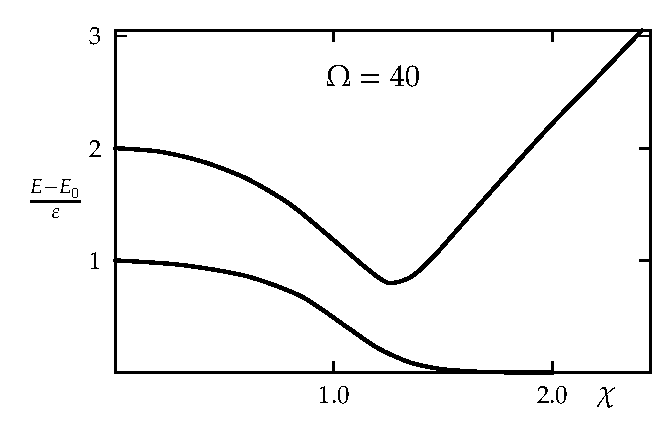
\includegraphics[width=0.75\textwidth]{pictures/10_1}
\par\end{centering}
\caption{\label{fig:10.1}$\Omega=40$ 时第一和第二激发态的激发能量。（引自［Ho 73］。）}
\end{figure}

近似解与精确解无法区分。这并不十分令人惊讶，因为我们知道 GCM 能够产生精确结果（第 10.4 节），并且在该模型中对称动量展开和高斯重叠方法中忽略的项是$\mathcal{O}(1/\Omega)$的。

\subsection{多维情形}

为简便起见，到目前为止我们仅处理了一个生成坐标。在若干坐标$\boldsymbol{a}=(a_{1},\dots,a_{f})$的一般情况下，Kamlah［Ka
73］以及 Onishi 等人［OU 75］对范数重叠核采用了通用高斯拟设：

\begin{equation}
\mathscr{N}(\boldsymbol{a},\boldsymbol{a}')=\mathscr{N}\left(\boldsymbol{q}+\frac{\boldsymbol{s}}{2},\boldsymbol{q}-\frac{\boldsymbol{s}}{2}\right)=\exp\left(-\frac{1}{2}s^{2}(\boldsymbol{q},\boldsymbol{s})\right),\label{eq:10.142}
\end{equation}

其中$\boldsymbol{q}=\frac{1}{2}(\boldsymbol{a}+\boldsymbol{a}'),\boldsymbol{s}=\boldsymbol{a}-\boldsymbol{a}'$，且

\begin{equation}
s^{2}=\gamma_{ij}(\boldsymbol{q})s^{i}s^{j}\label{eq:10.143}
\end{equation}

是由坐标$\boldsymbol{a}$表征的弯曲空间中的测地距离平方。应用 Riemann 空间理论，人们可以如第 10.7.4
节那样推进，并最终得到集体 Hamiltonian：

\begin{equation}
\mathscr{H}_{\mathrm{coll}}=-\frac{1}{\sqrt{\gamma}}\frac{\partial}{\partial q^{i}}\sqrt{\gamma}\left(\frac{\hbar^{2}}{2M}\right)^{ij}\frac{\partial}{\partial q^{j}}+\tilde{V}(\boldsymbol{q}),\label{eq:10.144}
\end{equation}

其中$\gamma(\boldsymbol{q})$是由拟设 (10.143) 定义的度规张量$\gamma_{ik}$的行列式。惯性张量和势具有与式
(10.134) 等类似的形式：

\begin{align}
\left(\frac{\hbar^{2}}{2M(\boldsymbol{q})}\right)_{ij} & =\left.-\frac{1}{4}\left(\frac{\Delta}{\Delta q^{i}}\frac{\Delta}{\Delta q^{j}}h(\boldsymbol{q},\boldsymbol{q}')-\frac{\Delta}{\Delta q^{i}}\frac{\Delta}{\Delta q'^{j}}h(\boldsymbol{q},\boldsymbol{q}')\right)\right|_{\boldsymbol{q}=\boldsymbol{q}'},\nonumber \\
V(\boldsymbol{q}) & =\tilde{V}(\boldsymbol{q})-\epsilon_{0}(\boldsymbol{q});\quad\tilde{V}(\boldsymbol{q})=\langle\boldsymbol{q}|H|\boldsymbol{q}\rangle,\nonumber \\
\epsilon_{0}(\boldsymbol{q}) & =\gamma_{ij}\left(\frac{\hbar^{2}}{2M}\right)^{ij}+\frac{1}{8}\gamma^{ij}\frac{\Delta}{\Delta q^{i}}\frac{\Delta}{\Delta q^{j}}\tilde{V}(\boldsymbol{q}),\label{eq:10.145}
\end{align}

其中$\Delta/\Delta q^{i}$是张量场的协变微商，例如在［LL 59, 卷 II, 第 10 章］中所定义的。动能算符类似于我们从
Pauli 量子化中得到的算符［式 (1.53)］。然而在后一种情况下，惯性张量与度规张量是相同的。现在我们必须区分完全由运动学性质（即由$\mathscr{N}$）决定的度规，与由$\mathscr{H}$的动力学行为给出的惯性。

\section{集体坐标的选取}

在第 10.4 节中我们看到，如果我们选取足够多的生成坐标，拟设 (10.2) 原则上包含了多体问题的精确解答。不幸的是，这是一个大到无法精确处理的问题，在实践中我们每次仅限于处理一个或也许少数几个生成坐标。因此，选取适当的生成坐标——即最合适的集合$|q\rangle=|\Phi(q)\rangle$——是非常重要的。在下文中，我们再次将自己限制在具有时间偶函数$|q\rangle$的实坐标$q$上。

生成函数集$|\Phi(q)\rangle$代表了多维能量曲面

\[
E[\Phi]=\langle\Phi|H|\Phi\rangle
\]

中的一条路径。为了确定这条路径，我们再次应用变分原理，并要求态

\begin{equation}
|\Psi\rangle=\int f(q)|\Phi(q)\rangle\,\mathrm{d}q\label{eq:10.146}
\end{equation}

中的能量期望值不仅关于权重函数$f$的变分是平稳的，而且关于路径$|\Phi(q)\rangle$也是平稳的。这种双重变分方法给出了我们一组耦合方程［HY
74, Vi 75］：

\begin{align}
\int\mathrm{d}q'\,\langle\Phi(q)|H-E|\Phi(q')\rangle f(q') & =0,\label{eq:10.147a}\\
\int\mathrm{d}q\,\mathrm{d}q'\,f^{*}(q)\langle\delta\Phi(q)|H-E|\Phi(q')\rangle f(q') & =0,\label{eq:10.147b}
\end{align}

它们原则上必须通过迭代来求解。

在点$q$处，变分$|\delta\Phi\rangle$并非完全任意。我们只能允许与路径本身正交的改变$|\delta\Phi\rangle_{\perp}$。平行于路径的变分可以被吸收到权重函数的变分中。

由于$|\delta\Phi\rangle_{\perp}$的长度是任意的，式 (10.147b) 可以写为

\begin{equation}
\int\mathrm{d}q'\,\prescript{}{\perp}{\langle}\delta\Phi(q)|H-E|\Phi(q')\rangle f(q')=0.\label{eq:10.148}
\end{equation}

在下一步中，我们做两个基本假定：

(i) 我们再次利用重叠函数$\langle\Phi(q)|\cdots|\Phi(q')\rangle$在$q=q'$处呈现尖锐峰值的事实，使得对于固定的$q$，仅有某个$q'$区域对积分
(10.148) 有贡献。

(ii) 我们假定在这一$q'$区域内，路径弯曲得不太强烈，使得$|\delta\Phi(q)\rangle$在这整个区域内都与路径正交。

在这些条件下，第二个方程 (10.147b) 与第一个方程 (10.147a) 解耦，并且对于不改变$|\Phi\rangle$范数的变分$|\delta\Phi\rangle_{\perp}$［Vi
75］，我们发现：

\begin{equation}
\prescript{}{\perp}{\langle}\delta\Phi|H|\Phi\rangle=0.\label{eq:10.149}
\end{equation}

变分$|\delta\Phi\rangle_{\perp}$受限于与路径正交。平行于路径的变分由下式给出：

\begin{equation}
|\delta\Phi\rangle_{\parallel}=|\Phi(q+\delta q)\rangle-|\Phi(q)\rangle=-\delta q\frac{\mathrm{i}}{\hbar}\hat{P}|\Phi(q)\rangle.\label{eq:10.150}
\end{equation}

算符$\hat{P}$是多体 Hilbert 空间中$-(\hbar/\mathrm{i})\partial/\partial q$的表象。它作用在$|\Phi\rangle$中的粒子坐标上，而不作用在参数$q$上。与路径正交的变分现在具有如下形式：

\begin{equation}
|\delta\Phi\rangle_{\perp}=|\delta\Phi\rangle-\hat{P}|\Phi\rangle\frac{\langle\Phi|\hat{P}|\delta\Phi\rangle}{\langle\Phi|\hat{P}^{2}|\Phi\rangle},\label{eq:10.151}
\end{equation}

其中$|\delta\Phi\rangle$是无限制的变分。势能$V(q)=\langle\Phi(q)|H|\Phi(q)\rangle$平行于路径的变分由下式给出：

\begin{equation}
\frac{\mathrm{d}V}{\mathrm{d}q}=+\frac{\mathrm{i}}{\hbar}\langle\Phi|[\hat{P},H]|\Phi\rangle,\label{eq:10.152}
\end{equation}

而与路径正交的变分必须消失：

\begin{equation}
\prescript{}{\perp}{\langle}\delta\Phi|H|\Phi\rangle=\left\langle \delta\Phi\middle|H-\frac{\hbar}{2\mathrm{i}}\frac{\mathrm{d}V}{\mathrm{d}q}\frac{\hat{P}}{\langle\Phi|\hat{P}^{2}|\Phi\rangle}\middle|\Phi\right\rangle =0.\label{eq:10.153}
\end{equation}

在导出该方程时，我们使用了式 (10.152) 以及$|\Phi\rangle$为时间偶的事实。问题 (10.153) 是一个有约束的变分原理，但约束算符不是
Hermite 的；因此我们将自己限制在$\hat{P}$可以被分解的情形：

\begin{equation}
\hat{P}=\mathrm{i}(A^{\dagger}-A),\quad\text{其中 }A|\Phi\rangle=0.\label{eq:10.154}
\end{equation}

例子是 Slater 行列式$|\Phi(q)\rangle$，此时我们有$A^{\dagger}=(1/\mathrm{i})\sum_{mi}P_{mi}a^{\dagger}_{m}a_{i}$；或者是
RPA 波函数，其中$A^{\dagger}$是玻色子的产生算符（亦参见［ABC 77b］）。

在此类情况下，我们可以定义一个 Hermite 约束算符：

\begin{equation}
\hat{Q}=\frac{\hbar}{2\langle\Phi|\hat{P}^{2}|\Phi\rangle}(A^{\dagger}+A),\label{eq:10.155}
\end{equation}

并由式 (10.152) 和 (10.153) 得到

\begin{equation}
\left\langle \delta\Phi\middle|H-\frac{\mathrm{d}V}{\mathrm{d}q}\cdot\hat{Q}\middle|\Phi\right\rangle =0,\label{eq:10.156}
\end{equation}

这给出了我们最优路径。它以如下方式确定：能量曲面关于垂直于路径的所有变分都具有极小值。这意味着，例如，它沿着裂变谷的底部行进（参见第
7.6 节）。式 (10.156) 是一个带约束的变分问题。约束算符$\hat{Q}$不是强加给系统的，而是由系统本身自洽决定的。它不会将系统推入非物理区域，而是像
d'Alembert 意义下的惯性力一样起作用［Vi 77］。

$|\Phi(q)\rangle$的实际计算需要双重迭代：从约束算符的某个初始值$\hat{Q}_{0}$开始，我们必须通过约束
HF 计算来确定$|\Phi_{0}(q)\rangle$。在第二步中，我们必须在每个点$q$处计算算符$\hat{P}$。例如，这可以通过在线性响应理论中求解式
(8.106) 来完成［参见式 (8.136) 和 (12.120)］。由算符$\hat{P}$可以确定新的约束$\hat{Q}$。这必须持续进行直到实现收敛。

最后，我们必须针对已确定的生成函数$|\Phi(q)\rangle$求解 Hill-Wheeler 方程 (10.5)。

这种双重迭代自然是极其耗时的，在 GCM 中自洽约束的规定迄今仅在三能级 Lipkin 模型［HY 74］以及$s-d$壳［PL
77］中进行了检验，并取得了相当有希望的结果。对于更重的核，第 7 章中描述的梯度方法可以简化该问题。

\section{GCM 在束缚态中的应用}

在过去几年中，GCM 已被应用于核结构的许多问题，例如巨共振、形状振动和对振动，以及核裂变和重离子碰撞（参见第 12 章）。方程 (10.5)
通常通过离散化求解。在许多情况下，只要在数值上消除范数的零本征值，极少数的网格点就已足够。在下文中我们仅讨论少数几个例子。

\subsection{巨共振}

轻核中的呼吸模和四极振荡已使用变形振子函数的 Slater 行列式$\Phi_{JM,P}(b,\beta)$进行了研究，这些基矢被投影到好角动量$J,M$和线动量$P=0$；它们依赖于振子长度$b=(b^{2}_{x}b_{z})^{1/3}$和形变$\beta=b_{x}/b_{z}$［CBA
73, AC 75］。对于$\beta=1$，参数$b$描述了径向坐标的标度变换，因此对应于呼吸模。（Ferrell 和 Visscher
在早期的一篇论文中就已使用过它［FV 56］）。坐标$\beta$描述了四极振荡。Hill-Wheeler 方程 (10.5) 采用
Brink 和 Boeker 相互作用［BB 67］通过离散化（多达 50 个网格点）求解。每个$J$值的最低本征态给出了基态转动带。它与投影
HF 波函数非常吻合。激发态是振动。人们在能谱以及跃迁矩中发现了非简谐性，以及不同模式之间的耦合。

Faessler 等人［KRG 76］以约束 HF 波函数$\Phi(r_{p},r_{n})$作为生成态，研究了满壳核$^{16}\mathrm{O}$、$^{40}\mathrm{Ca}$、$^{90}\mathrm{Zr}$和$^{208}\mathrm{Pb}$中的单极模式。坐标$r_{p},r_{n}$是质子和中子的均方根半径，约束算符（参见第
7 章）由下式给出：

\[
r^{2}\left(1+\exp\left(\frac{r-R}{a}\right)\right)^{-1}.
\]

Fermi 分布确保了约束算符是有界的，相应的 HF Hamiltonian 具有分立本征态。与连续谱的耦合被忽略。相互作用是 Skyrme
类型的修正$\delta$相互作用，在此情况下重叠积分$\mathscr{H}$可以以简单的方式计算。通过约束 HF 计算，标度规定可以得到检验，并发现它是完全合理的。方程
(10.5) 再次通过离散化求解。GCM 的基态能量与 HF 能量非常吻合。激发态是呼吸模。表 10.1 给出了一些结果。

\begin{table}[htbp]
\caption{\label{tab:10.1}呼吸模的 GCM 计算结果：激发能量$E$、约化跃迁几率、能量加权求和规则 (8.154) 的份额$S$、质子和中子跃迁振幅$A_{p}$与$A_{n}$、同位旋期望值$\langle T^{2}\rangle$以及质子和中子半径$r_{p}$与$r_{n}$。（引自［KRG
76］。）}

\centering{}%
\begin{tabular}{ccccccccc}
\toprule 
核素 & $E\,(\mathrm{MeV})$ & $B(E0)\,(\mathrm{fm}^{4})$ & $S$ & $A_{p}\,(\mathrm{fm}^{2})$ & $A_{n}\,(\mathrm{fm}^{2})$ & $\langle T^{2}\rangle$ & $r_{p}\,(\mathrm{fm})$ & $r_{n}\,(\mathrm{fm})$\tabularnewline
\midrule
$^{16}\mathrm{O}$ & 0 &  &  &  &  & 0.00 & 2.70 & 2.67\tabularnewline
 & 23.96 & 106 & 0.56 & 10.3 & 9.7 & 0.00 & 2.91 & 2.86\tabularnewline
$^{40}\mathrm{Ca}$ & 0 &  &  &  &  & 0.02 & 3.41 & 3.36\tabularnewline
 & 20.73 & 502 & 0.55 & 22.4 & 20.4 & 0.14 & 3.50 & 3.44\tabularnewline
$^{90}\mathrm{Zr}$ & 0 &  &  &  &  & 30.12 & 4.22 & 4.30\tabularnewline
 & 17.46 & 1530 & 0.45 & 39.1 & 49.8 & 30.12 & 4.25 & 4.33\tabularnewline
$^{208}\mathrm{Pb}$ & 0 &  &  &  &  & 506.38 & 5.46 & 5.66\tabularnewline
 & 13.32 & 5749 & 0.36 & 75.8 & 127.4 & 506.41 & 5.47 & 5.67\tabularnewline
 & 21.29 & 359 & 0.04 & -19.0 & 130.6 & 506.59 & 5.45 & 5.71\tabularnewline
 & 38.18 & 239 & 0.04 & -15.4 & 26.3 & 506.68 & 5.44 & 5.79\tabularnewline
\bottomrule
\end{tabular}
\end{table}

$^{208}\mathrm{Pb}$中同标呼吸模的能量为 13.32 MeV，与不可压缩性（式 (5.95)）$K\sim200\,\text{MeV}$的液滴模型以及采用
Migdal 力的 RPA 计算［RS 74a］非常吻合。

带有可变振子参数的振子波函数基底中的 Skyrme 相互作用（参见第 4.4.3 节）为$\mathscr{H}$和$\mathscr{N}$提供了相当简单的解析表达式。它们被
Giraud 和 Grammaticos［GG 75］结合矩展开（参见第 10.7 节）用于单极模式的描述。Flocard 和 Vautherin［FV
75, 76］利用振子波函数的 Slater 行列式和 Skyrme 力，通过离散化（多达 143 个网格点）求解了单极、四极和偶极激发的
HW 方程 (10.5)：基态再次与 HF 态非常吻合。图 10.2 显示了$^{16}\mathrm{O}$中基态 ($g_{0}$)
和前两个激发呼吸模 ($g_{1},g_{2}$) 的权重函数$g_{i}$［式 (10.12)］，以及能量重叠核的对角部分（式
(10.135) 中的$\mathscr{H}(r,r)$），它大致对应于集体坐标的势$V(r)$。我们看到函数$g_{i}$在此势中的定性行为类似于振子函数。

\begin{figure}[htbp]
\begin{centering}
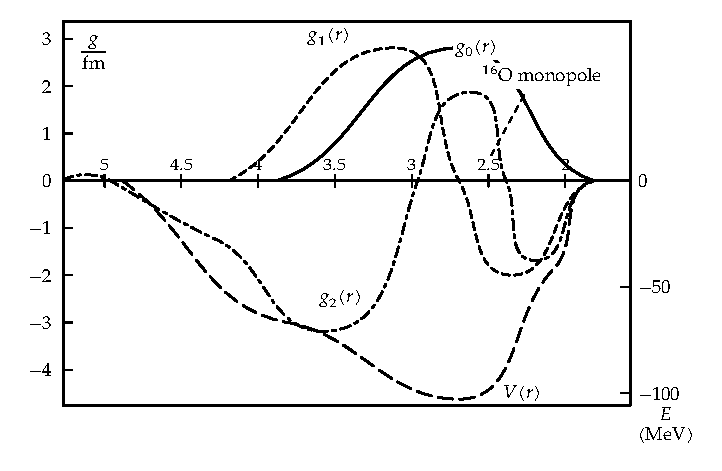
\includegraphics[width=0.75\textwidth]{pictures/10_2}
\par\end{centering}
\caption{\label{fig:10.2}单极振动情形下$^{16}\mathrm{O}$中前三个 GCM 态的权重函数$g_{i}$以及能量重叠核的对角部分$V(r)$。（引自［FV
76］。）}
\end{figure}

随着质量数的增加，函数$g_{0}$的宽度减小。对于重核，它在生成坐标的某个确定值处呈现尖锐的峰值。这意味着 GCM 波函数在很好近似下由带有该参数的
Slater 行列式给出。

GCM 也已被应用于轻核中的低激发形状振动。只要我们将它们限制在仅包含$s\text{-}d$壳的组态空间［GMA 75, MMR
75］，它们就可以与该子空间中 Hamiltonian 的精确对角化［PW 72, Wh 72, SZ 72］进行比较，并且发现许多能级都符合得很好。然而在某些情况下，符合得相当差。这意味着相应的态并不落在由生成函数张成的空间中。纯四极约束［KK
74］的效果此时不如第 10.8 节所讨论的由系统本身决定的约束算符［PL 77］。

\subsection{对振动}

在第 8.8 节中我们看到，在基于正常流体基态的 RPA 对对振动的描述中，对于临界耦合常数$G_{c}$我们发现了相变。在这一区域，RPA
和 BCS 模型都不能很好地工作。GCM 提供了一种克服这一困难的方法。

若干作者［JMR 72, ISY 73］提出使用投影到好粒子数的 BCS 波函数［参见式 (6.31)］（参见第 11.4 节）作为生成态：

\begin{equation}
|\Phi^{N}\rangle=P^{N}\prod_{\alpha,m}\left(u_{\alpha}+v_{\alpha}a^{\dagger}_{\alpha m}a^{\dagger}_{\alpha-m}\right)|-\rangle,\label{eq:10.157}
\end{equation}

其中$P^{N}$是向粒子数$N$的投影算符，而$\alpha=(nlj)$是不同$j$壳的量子数。对于独立参数$p_{\alpha}=u_{\alpha}/v_{\alpha}$，这些态张成了全
Hilbert 空间的高级数等于零（seniority-zero）子空间（参见第 6.2 节和［JMR 69］）。对于仅依赖于一个参数$\Delta$的
BCS 形式 (6.59) 的占据几率$u_{\alpha},v_{\alpha}$，这在很好近似下仍然成立。由于我们期望具有$J^{\pi}=0^{+}$的对振动落在该子空间中（参见第
8.8 节），拟设 (10.157) 对于在 GCM 框架内描述它们特别有用。第二个参数，即化学势$\lambda$，可以通过每个$\Delta$网格点处的
BCS 粒子数方程 (6.53) 来确定，或者可以作为第二个生成坐标使用（Sorensen 等人［SS 72b］）。

该方法对于超导核、非超导核以及过渡区域同样有效。它已被采用纯配对力［SS 72b, FGP 73］应用于简单模型以及 Pb、Ni 和
Sn 区域中的对振动能谱。

图 10.3 显示了$^{208}\mathrm{Pb}$基态以及 4.87 MeV 处所谓的对振动态的 GCM 波函数组分，后者在很大程度上是一个$2p\text{-}2h$态，或者是$^{210}\mathrm{Pb}$中$2p$对振动与$^{206}\mathrm{Pb}$中$2h$对振动的叠加。$0p\text{-}0h$、$2p\text{-}2h$和$4p\text{-}4h$组分作为配对强度$G$的函数给出。给出正确质量差$M(^{206}\mathrm{Pb})+M(^{210}\mathrm{Pb})-2M(^{208}\mathrm{Pb})$的$G$的真实值为$G=0.1166\,\text{MeV}$。在此取值下，基态已经有
10\% 是$2p\text{-}2h$态，而对振动大致有 12\% 的$4p\text{-}4h$掺杂。

\begin{figure}[htbp]
\begin{centering}
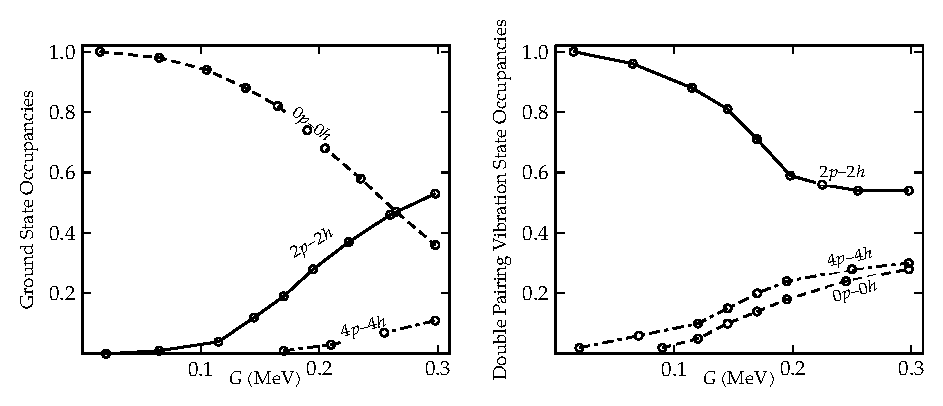
\includegraphics[width=0.85\textwidth]{pictures/10_3}
\par\end{centering}
\caption{\label{fig:10.3}$^{208}\mathrm{Pb}$基态与 4.87 MeV 处对振动态中$0p\text{-}0h$、$2p\text{-}2h$和$4p\text{-}4h$组分百分比随$G$的变化关系。（引自［SS
72b］。）}
\end{figure}

更逼真的核力已被 Faessler 等人［AGM 74］在$p\text{-}f$壳中使用。在此，式 (10.157) 中的 BCS
函数被约束 HFB 函数替换（参见第 7.6 节）。约束算符是可变强度的配对势，生成坐标是由此产生的能量贡献$-\frac{1}{2}\operatorname{Tr}(\kappa^{\dagger}\Delta\kappa)$。生成函数通过向好粒子数和角动量投影从这些
HFB 函数确定。结果与实验能级和转移截面符合良好。

该方法提供了一个研究基态和对振动态中配对关联（通过能隙$\Delta$衡量）对有效配对强度$G_{\mathrm{eff}}$的依赖关系的工具（图
10.4）。在基态强烈配对（大$G_{\mathrm{eff}}$）的情况下，对振动具有微弱的配对关联。例如在稀土核中就是如此。对于基态配对微弱的原子核，如
Ti，情况正好相反（亦参见［Kl 70］）。从第 7.7 节我们知道，Coriolis 反配对效应 (CAP) 随着角动量的增加降低了有效配对强度。这在稀土核的基态中产生降低的配对关联，并在对振动模式中产生增加的配对关联。然而对于较轻的核（如
Ti），这不再成立。

\begin{figure}[htbp]
\begin{centering}
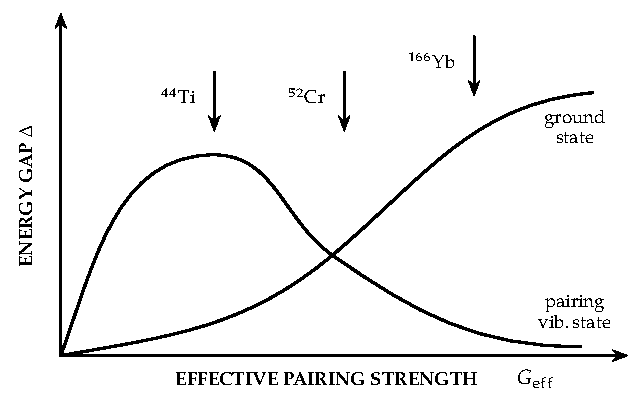
\includegraphics[width=0.75\textwidth]{pictures/10_4}
\par\end{centering}
\caption{\label{fig:10.4}能隙$\Delta$对有效配对强度$G_{\mathrm{eff}}$依赖关系的示意图。箭头指出了若干原子核的位置。（引自［GSF
75］。）}
\end{figure}

最后，如果我们引入更多的生成坐标，如形变参数$\beta$、配对参数$\Delta$等等［MAG 75］，我们可以通过 GCM
描述不同模式之间的各种耦合。我们甚至可以通过做出如下推广拟设来包含单粒子自由度［DMG 76, MGA 77］：

\begin{equation}
|\Psi\rangle=\int\mathrm{d}a\,f(a)|\Phi(a)\rangle+\sum_{i}\int\mathrm{d}a\,f^{i}(a)|\Phi_{i}(a)\rangle,\label{eq:10.158}
\end{equation}

其中$|\Phi(a)\rangle$例如是依赖于某个形变参数$a$的约束 HF 计算的基态，而$|\Phi_{i}(a)\rangle$是相应的$1p\text{-}1h$态，等等。



\chapter{对称性的恢复\label{chap:=005BF9=0079F0=006027=007684=006062=00590D}}

\section{引言}

在研究核相互作用的性质时（第4章），我们表明精确的多体Hamilton量 $H$ 在一些对称操作下是不变的，也就是说，它与相应的对称算符
$S$ 对易：
\[
[H,S]=0\tag{11.1}
\]

因此，我们总能找到同时是 $H$ 和 $S$ 本征函数的波函数。例如，线性动量 $\boldsymbol{P}$ 的三个分量、粒子数
$N$ 以及角动量算符 $\boldsymbol{J}^{2},J_{z}$ 。

我们还看到，这种一般性质在少数粒子的情况下非常有用，通过在对称算符的适当本征空间中工作，可以显著减小相应本征值问题的规模。两体系统中质心坐标的消除或应用于闭壳外少数粒子的角动量耦合技术就是例子。

在多粒子和强关联的一般情况下，对称性的恰当处理是一个严重的问题：一方面，我们想用简单的波函数来描述系统，比如独立运动粒子（或准粒子）的直积态；另一方面，如果我们同时要求恰当的对称行为，这样简单的波函数就无法考虑核子之间的重要关联。例如，唯一的平移不变直积波函数是平面波的乘积。它们肯定无法描述核子之间的强关联，正是这种关联导致它们聚集成一个有限的原子核。

然而在第2章中我们看到，这种关联可以用平均场（壳模型）来描述，并且壳模型波函数的直积态对许多核性质提供了非常合理的描述。然而，这样的波函数破坏了平移对称性。

这是一个普遍的过程\footnote{关于这一点的更详细讨论，见\cite{Li60a}}，在核物理中非常重要，即通过违反对称性的平均场方法来处理关联。这样的描述是否可行以及是否是一个好的近似当然取决于关联的性质。导致稳定形变的长程粒子-空穴关联以及提供超流性质的粒子-粒子关联，在任何情况下都是平均场类型的。在第7章中我们看到，它们可以用HFB理论来处理，这是一种违反角动量和粒子数守恒的平均场方法。结果表明，关联越强，这种近似就越好。类似于固体物理，我们说系统经历了向违反对称性状态的相变，例如向形变状态或超流相的相变。当然，当我们说原子核是局域化的、形变的或具有超流相时，经典和宏观的考虑进入了我们的论证。在本章后面我们将看到，相变的平均场描述在非常大（宏观）的系统中最终会变得精确。这意味着对于某些可测量的量，我们是在违反对称性的平均场方法中计算它们还是在不违反对称性的理论中计算它们可能无关紧要，当然，从量子力学原理上讲，后者是必需的。想象一个具有各种粒子数的量子流体$^{3}\mathrm{He}$的液滴。一旦液滴大到实际上可以“看到”，将液滴（或其平均场）视为局域化的（波包）肯定是一种精确的描述，尽管量子力学对于定态仍然需要平移不变的处理。

原子核当然不是宏观物体，但较重的原子核足够大，以至于对于宏观液滴最终会变得精确的平均场处理，对于某些量已经是非常好的描述。当然，这些量也是宏观定义的量，例如半径、形变\footnote{原子核的形变当然不像在宏观系统中那样是一个直接可测量的量，而只能以一种依赖模型的方式通过“内禀”四极矩相当间接地定义（见1.5节和附录B.2节）；一旦这种关系一劳永逸地建立起来，平均场理论在整个周期表中也能很好地再现原子核的形变。}、
超流电流、基态能量等。然而，那些具有量子性质的量，例如离散能谱和激发态之间的跃迁，将无法用纯平均场方法来描述。

特别地，直积波函数是对精确多体状态的一种非常糟糕的近似。正如我们将看到的，人们曾试图将违反对称性的波函数解释为在随原子核移动的“内禀”坐标系中的一个函数。所有仅依赖于这个内部函数的量最终在平均场方法中能得到很好的重现。

然而，有两个理由让我们寻找超越平均场的方法：
\begin{enumerate}
\item 在核物理学中，我们还对诸如跃迁概率和电磁矩等物理量感兴趣，而这些量绝不能仅从违反对称性的Nilsson波函数计算得出。
\item 原子核是一个有限系统。因此，相变总是会被抹平。我们经常会发现从守恒到弱破缺的逐渐转变，最终对称性会强烈破缺。在弱对称性破缺的情况下，我们必须超越平均场方法并恰当地纳入对称性。
\end{enumerate}
在11.2节中，我们首先希望更详细地讨论平均场方法中的对称性破缺机制。这将使我们更好地理解第5、6和7章中使用的方法。我们在此进行此讨论，是因为在那些章节中我们还没有第9和10章中的技术。

为了恢复在平均场方法中被破坏的对称性，人们尝试明确地转换到一个“内禀”系统。然而，这些尝试往往与基本困难紧密相连。另一方面，这些想法在许多唯象模型中被使用（见1.5节）。因此，我们将在11.3节中简要讨论它们。在从平均场方法获得的波函数基础上发展对称性守恒理论的常用方法是将波函数投影到对称算符的本征空间上。这些将在11.4节中讨论。

我们还将提到RPA近似。它超越了静态平均场方法，包含更高阶的关联，并提供对称性的近似恢复（见8.4.7节以及{[}UW 65, GW
68, MW 69b, MW 70, Bi 76, Ma 77a{]}）。正如我们将在12.3.2节中看到的，我们也可以在含时平均场理论中推导出这种方法，这表明这种更一般的平均场方法已经可以恢复对称性破缺的一些方面。

在本章中，我们主要探讨平移不变性（向局域化核的转变）、粒子数（向超流态的相变）和角动量（向形变态的相变）的对称性破缺。当然，还有其他对称性，如宇称\cite{BSB69}（在π介子凝聚的背景下{[}MKS
74, BF 74, BCD 75, BW 76{]}也会被打破）或同位旋（它只是一种近似对称性\cite{GW68}）。它们可以用非常相似的方式处理。

人们还研究了核物质具有由非平面波HF态描述的周期性长程有序晶体结构的可能性，这种结构违反平移对称性（Overhauser态{[}Ov
60, ALP 77, AAZ 77{]}）。人们发现，对于实际的核力，这样的波函数通常比平面波具有更高的能量。只有在非常低的亚核密度下，
$\alpha$粒子的稳定晶体结构才能形成（另见\cite{BC73}）。

本章讨论的对称性破缺是基于平均场方法的。当然，也有其他对称性破缺理论。它们有时可以用类似的技术来处理。

\section{平均场理论中的对称性破缺\label{sec:=005E73=005747=00573A=007406=008BBA=004E2D=007684=005BF9=0079F0=006027=007834=007F3A}}

正如我们在4.3节和第7章中所看到的，在原子核中存在非常不同的关联：一方面，存在非常短程的Brueckner关联，它与对称性破缺无关。另一方面，存在由ph和pp力引起的长程关联\footnote{然而，我们必须强调，这并不意味着产生这些关联的力的范围很大。}。
如果它们较弱，可以用RPA近似处理，并产生谐波集体振动和相关的基态。如果它们变得更强，我们会发现非谐性和能量大幅降低的模式（软模式）。相应的能量面在一个方向上变得非常平坦，并且在足够强的关联下，会出现突然的对称性破缺最小值。在这种情况下，\ref{chap:=0063A8=005E7F=007684=005355=007C92=005B50=006A21=00578B=00FF08HFB=007406=008BBA=00FF09}中讨论的平均场近似会产生非零的形变势
$\Gamma$ 或配对场 $\Delta$ 作为非线性“能隙方程”的解：

\[
\Gamma_{lm}=\sum_{rs}v^{\text{ph}}_{lsmr}\rho_{rs},\;\Delta_{lm}=\sum_{rs}v^{\text{pp}}_{lmrs}\kappa_{rs}\tag{11.2}
\]

其中$v^{\text{ph}}$和$v^{\text{pp}}$分别是ph和pp通道中的有效力，密度$\rho$和$\kappa${[}\ref{eq:=005355=007C92=005B50=005BC6=005EA6=0077E9=009635}{]}通过HFB方程\ref{eq:HFB equation}的对角化非线性地依赖于$\Gamma$和$\Delta$。

由于密度$\rho$和$\kappa$是用对称性破缺的波函数计算的，它们有一个单极部分$\rho_{0},\kappa_{0}$
、一个四极部分$\rho_{2},\kappa_{2}$等等。它们是通过将指标$r$和$s$耦合到角动量$I=0,2,\ldots$得到的，$\rho_{0}$对应于球形密度分布，并产生势$\Gamma$的球形部分$V_{0}$
。这在所有原子核中都很明显，对应于球形壳模型势。在下面我们将在此基础上进行研究。

取决于相互作用$v^{\text{ph}}$和$v^{\text{pp}}$的强度以及费米面附近的能级密度，“能隙方程”对于四极部分$\Gamma_{2}$
、单极配对场$\Delta_{0}$以及最终对于更高阶项也可能有非零解，这些在原子核中不太重要\footnote{例如，八极形变（$\Gamma_{3}$）或四极配对（$\Delta_{2}$）；另见4.4.7节中的多极展开。}。因此，我们可以将平均场分为三部分，
$V_{0}$ ，$\Gamma_{2}$和 $\Delta_{0}$ 。它们与平移对称性、转动对称性和粒子数的破坏有关。

在4.4.7节中我们看到，我们可以将相互作用 $v^{\text{ph}}$ 和 $v^{\text{pp}}$ 分解为具有不同角动量的分量。根据式（4.124）和（4.131），它们在角度上是可分离的。由于径向依赖性仅在核表面附近出现，我们可以用一个常数很好地近似它，对于$v^{\text{ph}}$的四极部分得到，并且从$v^{\text{pp}}$的单极部分得到著名的配对加四极模型（见7.4节）），我们将在下面关于原子核相变的讨论中使用它。

我们首先研究四极关联。在这种情况下，导致一体方程（11.2）的有效两体Hamilton量可以写成以下形式

\[
H=\sum_{k}\epsilon_{k}c^{\dagger}_{k}c_{k}-\frac{\chi}{2}\sum_{\mu}Q^{\dagger}_{\mu}Q_{\mu};\;\chi>0\tag{11.3}
\]

$c^{\dagger}_{k},c_{k}$ 是球形壳模型基中的粒子算符， $\epsilon_{k}$ 是 $T+V_{0}$
的相应本征值。四极算符$Q_{\mu}$由下式给出

\[
Q_{\mu}=\sum_{k_{1}k_{2}}\langle k_{1}|r^{2}Y_{2\mu}|k_{2}\rangle c^{\dagger}_{k_{1}}c_{k_{2}}\tag{11.4}
\]

“形变”方程（11.2）现在具有式（7.75）的形式，并确定形变参数 $q_{\mu}$ ：

\[
q_{\mu}=\chi\langle\Phi|Q_{\mu}|\Phi\rangle\tag{11.5}
\]

为了避免开壳层中HF的问题，我们进一步假设对于零相互作用 $\left(\chi=0\right)$ ，具有 $\epsilon_{i}\leq\epsilon_{F}$
的球形子壳层 $i$ 被占据，而具有 $\epsilon_{m}>\epsilon_{F}$ 的子壳层 $\epsilon_{m}$
是空的。

对于非零相互作用，系统的行为在很大程度上取决于费米面附近的平均能级间距\footnote{见6.3.5节中关于 $\Delta$ 的类似讨论。}
与强度 $\chi$ 的关系。例如，对于小的能级密度，对于幻核，或者对于 $\chi$ 的小值，我们有球形原子核的情况。“形变”方程（11.5）只有解
$q_{\mu}=0$ 。它对应于能量表面的一个最小值，我们可以在RPA框架{[}式（8.135）{]}中用频率 $\Omega$
计算振动状态：

\[
\frac{1}{\chi}=\sum_{mi}\left|\langle m\|r^{2}Y_{2}\|i\rangle\right|^{2}\frac{2(\epsilon_{m}-\epsilon_{i})}{(\epsilon_{m}-\epsilon_{i})^{2}-(\hbar\Omega)^{2}}\tag{11.6}
\]

随着能级密度的增加（即，如果我们研究远离封闭主壳层的原子核）或对于增加的强度 $\chi$ ，我们会达到一个点，此时RPA能量变为零，这等同于式（11.5）的球形解
${q}_{\mu}=0$ 不再对应于能量表面的最小值（见8.4.3节）。式（11.5）至少存在一个形变解 $\left|\Phi_{0}\right\rangle $
，其具有

\[
\langle\Phi_{0}|Q_{\mu}|\Phi_{0}\rangle\neq0\text{（至少对某个 }\mu\text{）}\tag{11.7}
\]

它违反了转动对称性。例如，我们现在能够通过函数$\left|{\Phi}_{0}\right\rangle $中质量分布的主轴来定义一个内禀坐标系。同时我们看到，现在有一整套HF方程的解$|\Phi\left(\Omega\right)\rangle$
，它们是通过由Euler角$\Omega=\left(\alpha,\beta,\gamma\right)$表征的空间任意转动从$\left|\Phi_{0}\right\rangle $得到的{[}见式（A.4）{]}

\[
\left|{\Phi\left(\Omega\right)}\right\rangle =\widehat{R}\left(\Omega\right)\left|{\Phi}_{0}\right\rangle \tag{11.8}
\]

如图11.1示意性所示。

\begin{figure}[H]
\begin{centering}
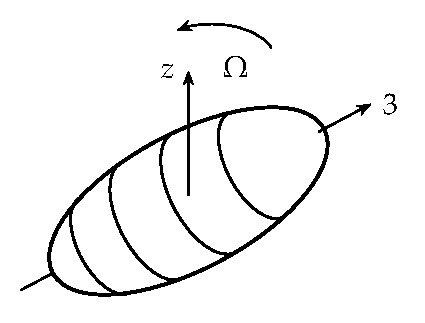
\includegraphics[width=0.48\linewidth]{pictures/11_1}
\par\end{centering}
\centering{}\caption{\label{fig:11_1}平均场方法定义一个内禀坐标系这一事实的示意表示。}
\end{figure}

由于Hamilton量的转动不变性，所有这些解具有相同的能量

\[
\langle\Phi\left(\Omega\right)\left|H\right|\Phi\left(\Omega\right)\rangle=\left\langle {{\Phi}_{0}\left|H\right|{\Phi}_{0}}\right\rangle .\tag{11.9}
\]

特别地，这意味着形变态不对应于最小值，而是对应于能量表面谷底的一个点。在11.4节中我们将看到，这种能量简并可用于构建所有这些波函数
$|\Phi\left(\Omega\right)\rangle$ 的线性叠加，它随后是对称算符 ${\boldsymbol{J}}^{2}$
和 ${J}_{z}$ 的本征函数。

从封闭主壳层附近的球形原子核到主壳层中间的形变原子核的转变通常称为相变。这类似于一个宏观系统，随着关联的增加我们有相同的机制：与对称性破缺相关的软模。然而，固态理论中的通常相变与核物理中的“相变”之间存在两个重要区别：

（i） 在宏观系统中，转变是严格不连续的，即不同的量（序参量）在连续参数的某个值处突然变化。对于有限系统，尖锐的转变被抹平，观察到由形变
${q}_{\mu}$ （或能隙 $\Delta$ ）给出的序参量有或多或少的逐渐变化。如果遵循我们的程序，这个事实有点隐藏起来：如果我们在RPA中围绕球形计算振动，我们发现随着耦合强度
$\chi$ 的增加，一个频率在尖锐的临界值 ${\chi}_{c}$ 处变为零。对于所有值 $\chi>{\chi}_{c}$
，我们找到一个形变解。然而，在有限系统中，两种方法——球形情况下的RPA和形变情况下的形变HF方法——在临界点附近失效，并且没有提供定量描述转变的方法。在一个精确解中，如图11.2示意性所示，我们发现在转变区域振动模的能量急剧降低，并在形变区域转变为
${2}^{+}$ 转动态，该转动态仅在非常大的形变或强关联的极限下变为零。

\begin{figure}[H]
\begin{centering}
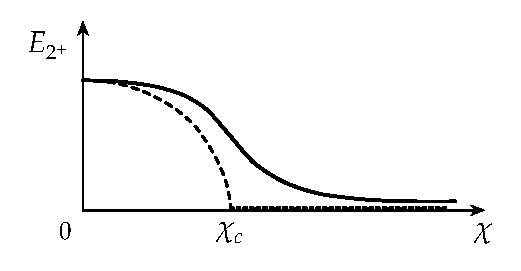
\includegraphics[width=0.5\linewidth]{pictures/11_2}
\par\end{centering}
\centering{}\caption{\label{fig:11_2}最低激发能作为四极耦合强度的函数的示意表示：精确解（实线）以及球形基中的RPA方法（虚线）和形变基中的RPA方法（点线）。在后一种情况下，最低的RPA解是赝态，它对应于转动（见8.4.7节）。}
\end{figure}

（ii） 在宏观情形下，平均场近似能够精确描述许多物理量，但在有限核系统中情况并非如此。正如我们将在11.4.4节中看到的，该近似仅在强对称性破缺的极限情况下才适用。在过渡区域存在许多原子核，静态平均场方法并不适用。从这个角度来看，线性动量、角动量和粒子数的三种对称性破缺非常不同。对于所有中等质量和重核，平均场近似在平移情形下的质量非常好。在转动情形下，它仅对形变良好的区域适用。然而，我们也观察到没有转动对称性破缺的球形核；也存在很大的过渡区域，平均场方法在那里失效。原子核中的BCS关联通常相当弱，因此相应的平均场近似，即BCS理论，往往不足以重现实验数据。因此，我们将在接下来的章节中研究改进平均场近似缺陷的方法。

四极关联强度的一种实验测量方法，因此也是平均场近似有效性的一种指示，由精确波函数 $|\Psi\rangle$ 中四极算符的涨落给出。

\[
\Delta{Q}^{2}=\langle\Psi\left|{Q\cdot Q}\right|\Psi\rangle-\langle\Psi\left|Q\right|\Psi\rangle\cdot\langle\Psi\left|Q\right|\Psi\rangle.\tag{11.10}
\]

（点表示五个四极算符的标量积。）由于在基态中期望值 $\left\langle {\Psi\left|{Q}_{\mu}\right|\Psi}\right\rangle $
在 $I=0$ 时为零，我们发现 $\Delta{Q}^{2}$ 与Hamilton量（11.3）的四极关联能成正比。

\[
\Delta{Q}^{2}=\langle\Psi\left|{\mathop{\sum}\limits_{\mu}Q^{\dagger}_{\mu}{Q}_{\mu}}\right|\Psi\rangle.\tag{11.11}
\]

四极力是吸引性的，因此系统希望在球形单粒子势 ${V}_{0}$ 中尽可能增加 $\Delta{Q}^{2}$ 。

另一方面，在实际原子核中存在关于 $\Delta{Q}^{2}$ 值的直接实验信息，因为它与非能量加权同位旋标量四极和规则成正比{[}见式（1.43）{]}。

\[
\Delta{Q}^{2}=\mathop{\sum}\limits_{\nu}{\left|\left\langle {\Psi}_{\nu}\parallel Q\parallel\Psi\right\rangle \right|}^{2}=5\cdot\mathop{\sum}\limits_{\nu}{BE2}\left({{2}^{+}_{\nu}\rightarrow0}\right).\tag{11.12}
\]

与能量加权和规则{[}式（8.159）{]}不同，能量加权和规则与 $\left\langle {r}^{2}\right\rangle $
成正比且大致为常数，非能量加权和在从球形到形变的转变过程中急剧增加：虽然巨四极共振的贡献大致保持不变，但最低 ${2}^{+}$
态的 ${BE2}$ 值从球形情形下的 $\sim{20}$ 单粒子单位{[}见式（B.85）{]}增加到形变情形下的 $\sim{100}$
，其中最低 ${2}^{+}$ 属于基态转动带。

四极强度在球形情形下集中在巨共振中，在形变情形下增加，然后集中在两个区域，即巨四极共振和集体转动。因此，在经典极限下，对于球形情形只有振动，而在形变情形下既有振动也有转动。

相变的进一步实验证据是“转动”谱的存在。在11.4节中我们将看到，在强对称性破缺的情况下，除了形变基态外，我们还得到一整个激发态带，它们与基态的区别仅在于对称算符
$S$ 的量子数。在那里，激发能与 ${S}^{2}$ 的本征值成正比。最简单的例子是形变核 $\left({\sim I\cdot\left({I+1}\right)/2\mathcal{G}}\right)$
中的转动带（$\sim I(I+1)/2\mathcal{J}$）、配对转动（$\sim(N-N_{0})^{2}/8\mathcal{I}_{N}$
\cite{Sch71a,BB76}）或平移激发（$\sim\boldsymbol{P}^{2}/2M$）。

相变也可以在玻色子图像中进行描述。一方面，我们在图9.5中看到，原则上我们可以通过费米子Hamilton量的玻色子展开来重现从球形到变形形状的转变。这些计算大多是在球形玻色子基中进行的。要在这个基中表示一个形变态需要非常复杂的波函数，因为我们总是在实验室坐标系中工作且不破坏转动对称性。另一方面，我们可以尝试用玻色子在内在坐标系中表示变形波函数：根据
Thouless 定理（E.26），我们可以用以下方式表示一个变形的Slater行列式。

\[
\left|{\Phi}_{0}\right\rangle =\mathcal{R}\exp\left({\mathop{\sum}\limits_{{mi}}{Z}_{mi}c^{\dagger}_{m}{c}_{i}}\right)|0\rangle,\tag{11.13}
\]

其中 $|0\rangle$ 是球形HF解， $\mathcal{R}$ 是归一化常数。在变形良好的情况下，我们有许多非零系数，即集体费米子对算符

\[
B^{\dagger}_{0}=\frac{1}{c}\mathop{\sum}\limits_{{mi}}{Z}_{mi}c^{\dagger}_{m}{c}_{i}\tag{11.14}
\]

其中

\[
{c}^{2}=\mathop{\sum}\limits_{{mi}}{\left|{Z}_{mi}\right|}^{2}
\]

在很好的近似下是一个玻色子（见9.2节），并且形变态

\[
|\Phi)=\mathcal{R}\exp(cB^{\dagger}_{0})|0)
\]

是一个仅包含集体玻色子 $B^{\dagger}_{0}$ 的相干态（见10.6.1节）。因此，我们将其称为玻色子 $B^{\dagger}_{0}$
的凝聚，类似于描述凝聚态物质某些类相变的玻色 - 爱因斯坦凝聚（另见\cite{SP77a}）。

对形变态的这种解释再次展示了平均场近似的经典行为。玻色子 $B^{\dagger}_{0}$ 的结构由变分方程（11.2）的解确定，一般来说它会随变形而变化。然而，我们可以证明，在小变形极限下，它恰好对应于RPA玻色子的
${ph}$ 部分，该部分在转变点处频率趋于零。从这个意义上说，我们可以说在相变过程中一个玻色子能量趋于零并形成凝聚。我们已经在BCS模型中使用了这个图像，在那里我们将BCS基态解释为Cooper对的凝聚。

到目前为止，我们的讨论主要集中在转动对称性的破坏上。接下来我们将表明，相同的考虑也可以应用于与配对关联相关的对称性破坏。这里我们首先研究简单的
辛弱数模型（见6.2节）。单个 $j$ 壳层中的有效Hamilton量由下式给出

\[
H=-G{S}_{+}{S}_{-}=-G\left({\boldsymbol{S}\cdot\boldsymbol{S}-{S}^{2}_{z}+{S}_{z}}\right),\tag{11.15}
\]

其中 ${S}_{i}$ 是在式（6.6）中定义的准自旋算符。它们作用于三维准自旋空间。 ${S}^{2}$ 和 ${S}_{z}$
与Hamilton量对易。因此，我们可以根据它们的辛弱数 $s$ {[}式（6.11）{]}和粒子数 $N$ 对本征态进行分类

\[
s=\Omega-{2S};\;\widehat{N}=2{S}_{z}+\Omega\tag{11.16}
\]

S由 $\Omega$ 个准自旋 ${\boldsymbol{s}}^{\left(m\right)}$ 组成{[}见图11.3和式（6.6）{]}。这个矢量的长度由辛弱数
$s$ 确定，并且我们将以下讨论限制在 $s$ 的一个固定值上。

\begin{figure}[H]
\begin{centering}
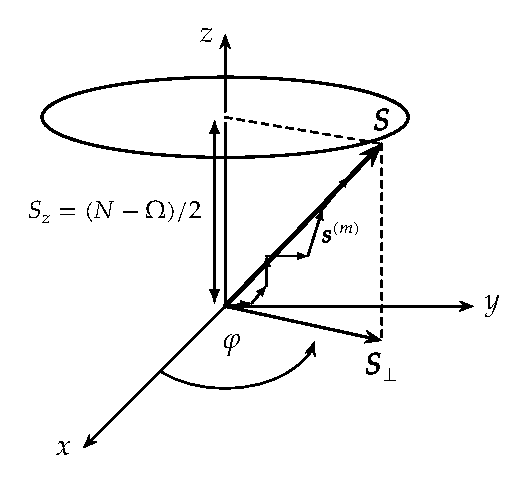
\includegraphics[width=0.46\linewidth]{pictures/11_3}
\par\end{centering}
\centering{}\caption{\label{fig:11_3}准自旋模型的示意图。}
\end{figure}

另一个量子数 ${S}_{z}$ 对应于绕 $z$ 轴的转动对称性。接下来我们将更详细地研究Hamilton量的这种不变性：

\[
\left\lbrack {H,\widehat{N}}\right\rbrack =0\text{ . }\tag{11.17}
\]

粒子数算符 $\widehat{N}$ 与 ${S}_{z}$ 相关（11.16），因此对应于准自旋空间中绕 $z$ 轴转动的无穷小生成元。这样的转动称为规范变换。相应的角度
$\varphi$ 是规范角。

我们可以用这个规范角表示算符 $\widehat{N}$

\[
\frac{\widehat{N}}{2}=-\frac{1}{i}\frac{\partial}{\partial\varphi}+\text{ const. }\tag{11.18}
\]

类似于用Euler角表示角动量算符 $\boldsymbol{J}$ ，如式（A.11）所示。

对于 $N$ 的固定值，即对于Hamilton量（11.15）的所有精确本征态 $|\Psi\rangle$ ，矢量S以频率

\[
\frac{d\varphi}{dt}=2\frac{dE}{dN}={2\lambda},\tag{11.19}
\]

绕对称轴进动，其中 $\lambda$ 是化学势{[}式（6.41）{]}。我们将这种运动称为配对转动。对于不同的粒子数，我们得到一个转动带（见图11.4）。

\begin{figure}[H]
\begin{centering}
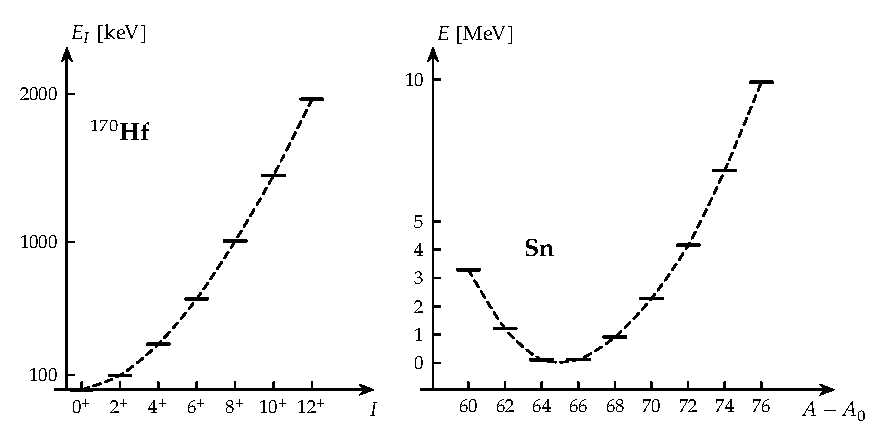
\includegraphics[width=0.62\linewidth]{pictures/11_4}
\par\end{centering}
\centering{}\caption{\label{fig:11_4}一个实验性的转动谱 $\left({^{170}\mathrm{{Hf}}}\right)$，其中激发能级对应于具有不同
$I$ 值的态，以及一个配对转动谱（Sn），其中“激发”能级对应于具有不同 $A$ 值的态（即相邻核中的基态）。（源自\cite{BB76}。）}
\end{figure}

${S}_{x}$ 和 ${S}_{y}$ 的期望值为零，

\[
\langle\Psi\left|{S}_{+}\right|\Psi\rangle=0,\tag{11.20}
\]

与上述讨论的情况中具有 $I=0$ 的精确基态的四极矩的方式相同。

$\boldsymbol{S}$ 在 $x,y$ 平面上投影的长度由下式给出

\[
{S}^{2}_{\bot}=\left\langle {\Psi\left|{{S}_{+}{S}_{-}}\right|\Psi}\right\rangle \tag{11.21}
\]

并且与关联能成正比。由于现在没有“球形”单粒子部分，系统在其基态总是倾向于 ${S}_{\bot}$ 的尽可能大的值，其中所有准自旋
${\boldsymbol{s}}^{\left(m\right)}$ 都是对齐的。因此，在这个模型中，对于所有力常数的值，我们都有一个“变形”态。对于大的
$S$ 值，即对于大的 $\Omega$ 值和 $N\ll\Omega$ ，我们因此可以预期通过打破规范对称性来获得精确波函数的良好近似。违反对称性的内态
$|\Phi\rangle$ 是一个BCS波函数。它由一个固定角度 $\varphi$ 表征。

\[
|\Phi(\varphi)\rangle=\mathop{\prod}\limits_{m>0}\left(u+ve^{\mathrm{i}\varphi}c^{\dagger}_{m}c^{\dagger}_{-m}\right)|-\rangle=e^{\mathrm{i}\varphi\widehat{N}/2}|\Phi(0)\rangle.\tag{11.22}
\]

通常的假设（6.31）对应于 $\varphi=0$ ，也就是说，我们以经典方式固定了角度。同样，所有态 $|\Phi\left(\varphi\right)\rangle$
在能量上是简并的。对称性破缺由能隙参数 $\Delta$ 来度量，它在转动情况下对应于变形方程（11.20）

\[
\Delta=G\left\langle {\Phi\left(0\right)\left|{S}_{+}\right|\Phi\left(0\right)}\right\rangle =G\mathop{\sum}\limits_{{m>0}}{uv}=G\cdot{\Omega uv}.\tag{11.23}
\]

系数 $u,v$ 由变分原理确定，这产生了通常的能隙方程{[}（6.60）和（6.65）{]}

\[
u=v=\frac{1}{\sqrt{2}}\tag{11.24}
\]

因此，BCS态也可以在准玻色子近似中由具有准玻色子 ${S}_{+}$ 的相干态来表示

\[
|\mathrm{BCS})=\mathcal{N}\exp(S_{+})|-)\text{ . }\tag{11.25}
\]

它违反了粒子数，但它具有适当粒子数 $N$ 的分量对应于系统的精确本征态（6.19）。对于大粒子数，相对涨落 ${\Delta N}/N$
（6.63）为零。因此，在这种情况下，平均场近似非常好。

在BCS理论更实际的应用中，除了单粒子部分外，我们还有纯配对力的模型

\[
H=\mathop{\sum}\limits_{k}{\epsilon}_{k}c^{\dagger}_{k}{c}_{k}-G\cdot P^{\dagger}P,\tag{11.26}
\]

\[
P^{\dagger}=\mathop{\sum}\limits_{{k>0}}c^{\dagger}_{k}c^{\dagger}_{k}
\]

现在不再可能有精确的解析解{[}KLM 61，RS 64，Ri 66{]}。它可以借助计算机求解，解表明BCS方法仍然是一个合理的近似，特别是如果我们只使用具有适当粒子数的分量（见第11.4节）。粒子数
$\widehat{N}$ 与Hamilton量对易；然而，相应的规范对称性被BCS近似打破，我们发现了一个相变。在所有细节上，该模型的工作方式与四极矩情况（11.3）完全类似。唯一的区别是我们现在必须对粒子数施加一个约束（通过在Hamilton量中添加一项
$-\lambda\widehat{N}$ ），因为我们对 $\widehat{N}$ 期望值为零的态不感兴趣。在转动对称性的情况下，我们有时也想要
${J}_{x}$ 期望值不为零的波函数。然后我们得到了转动模型（见第3.4节）。

为了展示从球形到变形的转变与从正常到超流系统的转变之间的紧密类比，我们给出以下相互对应的量的列表{[}Sch 71a，BHR 73{]}。

球形基中的模型Hamilton量是

\[
{H}_{Q}=\epsilon-\frac{\chi}{2}Q\cdot Q,\;{H}_{p}=\epsilon-GP^{\dagger}P.
\]

对于小耦合强度，基态是不相关联的球形壳模型态 $|0\rangle$ 。在RPA中考虑的剩余相互作用产生集体振动，即

四极振动 配对振动在

具有 $I=2$ 的核 质量为 $A\pm2$ 的核中。

它们增强了

BE2 值（在单对转移截面中

粒子单位）（以 ${2p}$ 单位）

${BE}\left({{2}^{+}\rightarrow{0}^{+}}\right)\simeq{20}{B}_{sp}\;\sigma\left({\text{ g.s. }\left({A-2}\right)\rightarrow\text{ g.s. }\left(A\right)}\right)\simeq{10}{\sigma}_{sp}.$

随着耦合强度增加，最低的RPA频率变为零。从这一点起存在一个

变形超流体

能量表面的最小值。它由基于球形（正常流体）基态 $|0\rangle$ 的直积波函数描述

\[
|\Phi\rangle=\mathop{\prod}\limits_{k}{\alpha}_{k}|0\rangle
\]

与准粒子算符

\[
\alpha^{\dagger}_{m}=\mathop{\sum}\limits_{k}{D}_{km}c^{\dagger}_{k},
\]

\[
\alpha^{\dagger}_{i}=\mathop{\sum}\limits_{k}{D}^{*}_{ki}{c}_{k},\;\alpha^{\dagger}_{i}={v}_{i}{c}_{i}+{u}_{i}c^{\dagger}_{i}.
\]

系数 ${D}_{kl}$ 和 ${u}_{k},{v}_{k}$ 由单粒子算符的对角化确定

\[
\epsilon-q\left({Q+Q^{\dagger}}\right),
\]

单粒子场的强度是序参量。它由“变形方程”和能隙方程自洽确定

\[
q=\chi\langle\Phi\left|Q\right|\Phi\rangle,\;\Delta=G\langle\Phi\left|P\right|\Phi\rangle.
\]

在准玻色子近似中，波函数 $|\Phi)$ 可写为相干态（玻色凝聚）

\[
|\Phi)\propto\exp(cB^{\dagger}_{0})|0),\quad|\Phi)\propto\exp(cA^{\dagger}_{0})|0),
\]

与玻色子

\[
B^{\dagger}_{0}=\frac{1}{c}\mathop{\sum}\limits_{{mi}}{Z}_{mi}c^{\dagger}_{m}{c}_{i},\;A^{\dagger}_{0}=\frac{1}{c}\mathop{\sum}\limits_{m}\frac{{v}_{m}}{{u}_{m}}c^{\dagger}_{m}c^{\dagger}_{m}+\frac{1}{c}\mathop{\sum}\limits_{i}\frac{{u}_{i}}{{v}_{i}}{c}_{i}{c}^{-}_{i}.
\]

平均场近似破坏了对称性。

\[
\left\lbrack {H,\widehat{J}}\right\rbrack =0,
\]

\[
\left\lbrack {H,\widehat{N}}\right\rbrack =0.
\]

其解 $|\Phi\rangle$ 表征了由坐标空间中的角度 $\Omega=\left({\alpha,\beta,\gamma}\right)$
以及准自旋空间中的角度 $\varphi$ 给出的一种取向。这些解对于转动是简并的

\[
R\left(\Omega\right)={e}^{{\mathrm{i}\alpha}{\widehat{J}}_{x}}{e}^{{\mathrm{i}\beta}{\widehat{J}}_{y}}{e}^{{\mathrm{i}\gamma}{\widehat{J}}_{z}},
\]

\[
G\left(\varphi\right)={e}^{{\mathrm{i}\varphi}\widehat{N}/2}.
\]

在形变状态下，我们在激发谱中有

$\beta,\gamma$ 振动 配对振动（含时形变）（含时能隙 $\Delta$ ）以及（作为无规位相近似法中的零频模式，见图11.4）

转动（具有 $I\neq0$ 的态） 配对转动（原子核中的基态）

\[
A\pm2,A\pm4,\ldots)\text{ . }
\]

基态“转动”带成员之间的跃迁与形变参数 $\left({q\text{ or }\Delta}\right)$ 的平方成正比。典型值为

\[
B\left({{E2},{2}^{+}\rightarrow{0}^{+}}\right)\simeq{100}{B}_{sp},\;\sigma\left({\text{ g.s. }\left({A-2}\right)\rightarrow\text{ g.s. }\left(A\right)}\right)\simeq{50}{\sigma}_{2p},
\]

\[
B\left({{E2},{2}^{\prime+}\rightarrow{0}^{+}}\right)\simeq3{B}_{sp},\;\sigma\left({\text{ g.s. }\left({A-2}\right)\rightarrow\text{ p. v. }\left(A\right)}\right)\simeq1{\sigma}_{2p}.
\]

转动可以（见11.4节）通过转动模型用经典方法处理：

\[
H-\omega{\widehat{J}}_{x},\;H-\lambda\widehat{N};
\]

或者通过投影用量子力学方法处理

\[
{P}^{I}_{MK}\propto\int{D}^{I*}_{MK}\left(\Omega\right)R\left(\Omega\right){\,\mathrm{d}\Omega},\;{P}^{N}\propto\int{e}^{-i\left({\varphi/2}\right)N}G\left(\varphi\right){d\varphi}.
\]

此列表总结了我们关于平均场理论中的对称性及其破缺的一般讨论，并且很明显，对于与对称性破缺相关的所有类型的相变，例如π介子凝聚，都可以列出类似的列表。我们现在将转向允许恢复破缺对称性的方法。

\section{向内禀系的变换\label{sec:=005411=005185=007980=007CFB=007684=0053D8=006362}}

\subsection{一般概念}

多体波函数中的对称性破缺与集体运动密切相关。为了更详细地解释这一事实，我们再次以转动对称性为例。一个形变波函数 $|\Phi\rangle$
在空间中定义了一个固定的取向，例如由质量分布的主轴来表征。所有仅在取向上与 $|\Phi\rangle$ 不同、但具有相同内禀结构并给出相同能量期望值的波函数
$|\Phi(\Omega)\rangle$ 都位于能量曲面的谷底。因此在经典图像中，我们有一种运动，如果它足够慢，就会靠近这个谷底。它对应于一种近似保持内禀结构的转动运动。如果形变很大，有许多粒子参与这种运动，我们就称其为集体运动。（关于这些准经典讨论的进一步内容，另见12.3节。）

在量子力学中，态 $|\Phi\left(\Omega\right)\rangle$ 跨越多体希尔伯特空间的一个子空间，即生成坐标方法（见第10章）意义下的集体子空间。如果这个子空间足够大——也就是说，正如我们将在11.4节中看到的，如果重叠
$\langle\Phi\left(\Omega\right)|\Phi\left({\Omega}^{\prime}\right)\rangle$
在 $\Omega={\Omega}^{\prime}$ 处强烈峰值化，这在强形变情况下会发生——它不仅大致包含基态，还包含具有相同内部结构且呈现转动谱的低激发态。

由于在这样一个波函数中的内禀结构在集体运动中大致保持，许多作者试图通过从 ${3A}$ 粒子坐标 ${\boldsymbol{r}}_{i}$
到集体坐标 ${q}_{1},\ldots,{q}_{f}$ 和内禀坐标 ${\xi}_{1}\ldots{\xi}_{{3A}-f}$
的适当坐标变换来分离内禀自由度和集体自由度{[}Vi 57a和b，Vi 58，SG 68，FKS 7{]}。

\[
\left({{\boldsymbol{r}}_{1},\ldots,{\boldsymbol{r}}_{A}}\right)\rightarrow\left({{q}_{1},\ldots,{q}_{f},{\xi}_{1},\ldots,{\xi}_{{3A}-f}}\right).\tag{11.27}
\]

集体坐标通常由基础对称性很好地定义为对称群生成元的正则共轭变量。在平移的情况下，有质心坐标；在转动的情况下，有一组角度作为Euler角；在超流体系中，它是规范角
$\varphi$ 。

内禀变量 $\xi$ 的定义是一个严重的问题。它仅在两个粒子的平移情况下很简单，此时它是相对坐标 $r={r}_{1}-{r}_{2}$
。在几个粒子的情况下，例如我们可以引入雅可比坐标，但在平移情况下的这个过程以及在转动情况下的类似过程在我们的多粒子系统中会变得极其复杂。然而，正如我们将在一些例子中看到的，我们有时可以在不明确指定内禀坐标的情况下推导出集体变量中的Hamilton量结构。

这些理论的主要思想是将核Hamilton量分解为以下三个部分

\[
H={H}_{\text{ coll }}\left(q\right)+{H}_{\text{ intr }}\left(\xi\right)+{H}_{\text{ coupl }}\left({q,\xi}\right),\tag{11.28}
\]

其中 ${H}_{\text{ coll }}$ 描述集体运动， ${H}_{\text{ intr }}$ 描述内禀运动。耦合项
${H}_{\text{ coupl }}$ ，希望它会很小或具有简单的结构。核平移的情况就是这个概念能很好发挥作用的一个例子。由于伽利略不变性，
${H}_{\text{ coupl }}$ 恒等于零。

如果我们可以忽略 ${H}_{\text{ coupl }}$ ，我们会发现总系统的本征函数是集体波函数 ${\chi}_{c}\left(q\right)$
和内禀波函数 ${\varphi}_{n}\left(\xi\right)$ 的乘积

\[
{\Psi}^{c}_{n}={\chi}_{c}\left(q\right)\cdot{\varphi}_{n}\left(\xi\right)\tag{11.29}
\]

并且能量具有以下形式

\[
{E}^{c}_{n}={E}_{c}+{E}_{n}.\tag{11.30}
\]

对于每个内禀态 ${\varphi}_{n}$ ，存在一个用指标 $c$ 标记的集体能带。

在这个过程的实际应用中，我们总是面临两个问题：

（i） 分解式（11.28）不是唯一的。它取决于内禀坐标的实际选择。显然，耦合项的大小敏感地依赖于这个选择。因此，有时会使用最小耦合变分原理来确定内禀系统{[}Co
56, BM 58, RV 69, Ru 73{]}。

（ii） 内禀Hamilton量 ${H}_{\text{ intr }}\left(\xi\right)$ 不依赖于 $A$
个粒子的 ${3A}$ 坐标，而仅依赖于 ${3A}-f$ 个变量 $\xi$ 。它们中没有一个能与粒子位置坐标等同。如果我们想在独立粒子图像中描述内禀运动，这就特别麻烦。在平移的情况下我们就已经有这个问题了。

因此，一系列作者使用了冗余变量的概念{[}LST 55, Li 55, Ta 56b, Na 57, Li 58, VC 70{]}。这里试图将正则变换方法的优点与处理
${3A}$ 个粒子坐标以描述内禀运动的优点结合起来。这是通过将 $A$ 体希尔伯特空间在粒子坐标 ${\boldsymbol{r}}_{1},\ldots,{\boldsymbol{r}}_{A}$
（物理子空间）中嵌入到一个维度为 ${3A}+f$ 的更大空间中来实现的，其中 $f$ 是集体变量的数量。我们用坐标 ${g}_{1},\ldots,{g}_{f}$
来表征这些额外的非物理自由度。然后物理子空间由以下条件表征

\[
{g}_{1}={g}_{2}=\cdots={g}_{f}=0.\tag{11.31}
\]

物理算符，即仅依赖于坐标 ${\boldsymbol{r}}_{1},\ldots,{\boldsymbol{r}}_{A}$ 的算符，例如Hamilton量，具有以下形式的本征函数

\[
{\Psi}_{mn}\left({g,\boldsymbol{r}}\right)={h}_{m}\left(g\right){\varphi}_{n}\left(\boldsymbol{r}\right),\tag{11.32}
\]

其中 ${h}_{m}\left(g\right)$ 是冗余坐标中的任意一组正交归一函数。因此，每个本征值 ${E}_{n}$
在扩大的空间中高度简并，但相应的本征函数在物理子空间（11.31）中是相同的\footnote{关于用冗余变量进行计算的更多细节，在量子力学情形下由 Lipkin 等人给出 \cite{LST55}，而对于经典理论由 Watanabe
给出 \cite{Wa56}。}。我们现在能够将冗余实验室系统中的坐标 ${g}_{1}\ldots{g}_{f},{\boldsymbol{r}}_{1}\ldots{\boldsymbol{r}}_{A}$
变换为具有集体坐标 ${q}_{1},\ldots,{q}_{f}$ 和粒子坐标 ${\boldsymbol{x}}_{1},\ldots,{\boldsymbol{x}}_{A}$
的冗余内禀系统中的坐标：

\[
{\boldsymbol{r}}_{i}={\boldsymbol{r}}_{i}\left({{q}_{1},\ldots,{q}_{f},{\boldsymbol{x}}_{1},\ldots,{\boldsymbol{x}}_{A}}\right),\;i=1,\ldots,A
\]

\[
{g}_{i}={g}_{i}\left({{q}_{1},\ldots,{q}_{f},{\boldsymbol{x}}_{1},\ldots,{\boldsymbol{x}}_{A}}\right),\;i=1,\ldots,f.\tag{11.33}
\]

通过这种方式，我们得到一个关于变量 $\boldsymbol{q}$ 和 $\boldsymbol{x}$ 的Hamilton量，其形式为

\[
H={H}_{\text{ coll }}\left(\boldsymbol{q}\right)+{H}_{\text{ intr }}\left(\boldsymbol{x}\right)+{H}_{\text{ coupl }}\left({\boldsymbol{q},\boldsymbol{x}}\right).\tag{11.34}
\]

在下一步中，我们对 ${H}_{\text{ intr }}$ 的对角化应用常规的近似技术。然而，问题仍然存在，即我们是否能找到一个合适的变换（11.33），使得耦合项很小，以及我们是否能以适当的方式分离通过这种近似得到的赝态的混合。在我们在平移和转动的背景下讨论这些技术之前，我们想提及类似的方法也已应用于更一般的集体运动，如表面振动，这些运动与对称性破缺无关{[}BP
53, Sü 54, MYT 55, To 55, MY 55, Co 55, MT 56, HM 57, Vi 57b{]}，但对于这些运动，人们也有兴趣推导集体Hamilton量。

\subsection{平移运动}

在下面我们将更详细地研究平移运动。这个简单的情形已经展示了许多问题。在核物理中，它与非常强的对称性破缺相关联。它是集体运动与内禀自由度完全解耦的唯一情形。其原因是伽利略不变性。

在这种情形下，内禀系统由质心参考系给出，集体坐标是

\[
\boldsymbol{R}=\frac{1}{A}\mathop{\sum}\limits_{i}{\boldsymbol{r}}_{i}\tag{11.35}
\]

在第一步中，我们不使用冗余坐标。在不指定内禀坐标 ${\xi}_{l}$ 的情况下，我们从（11.27）式得到导数

\[
\frac{\partial}{\partial{\boldsymbol{r}}_{i}}=\frac{1}{A}\frac{\partial}{\partial\boldsymbol{R}}+\mathop{\sum}\limits_{l}\frac{\partial{\xi}_{l}}{\partial{\boldsymbol{r}}_{i}}\frac{\partial}{\partial{\xi}_{l}}.\tag{11.36}
\]

由于内禀坐标 ${\xi}_{l}$ 仅依赖于差值 ${\boldsymbol{r}}_{i}-{\boldsymbol{r}}_{j}$
，我们得到 $\mathop{\sum}\limits_{i}\left({\partial/\partial{\boldsymbol{r}}_{i}}\right){\xi}_{l}=0$
并发现集体运动完全解耦

\[
H=-\frac{{\hbar}^{2}}{2m}\mathop{\sum}\limits_{i}{\left(\frac{\partial}{\partial{\boldsymbol{r}}_{i}}\right)}^{2}+V=\frac{1}{2Am}{\boldsymbol{P}}^{2}+\mathop{\sum}\limits_{{l{l}^{\prime}}}{D}_{l{l}^{\prime}}\left(\xi\right){\pi}_{l}{\pi}_{{l}^{\prime}}+V\left(\xi\right),\tag{11.37}
\]

质心动量为 $\boldsymbol{P}=\left({\hbar/i}\right)\partial/\partial\boldsymbol{R}$
，内禀动量为 ${\pi}_{l}=\left({\hbar/i}\right)\;\partial/\partial{\xi}_{l}$
，以及内禀惯性函数

\[
{D}_{l{l}^{\prime}}\left(\xi\right)=\mathop{\sum}\limits_{i}\frac{\partial{\xi}_{l}}{\partial{\boldsymbol{r}}_{i}}\cdot\frac{\partial{\xi}_{{l}^{\prime}}}{\partial{\boldsymbol{r}}_{i}}.\tag{11.38}
\]

如在上一节中所讨论的，我们不能用壳模型Hamilton量来近似（11.37）式的内禀部分。因此，我们现在应用冗余坐标方法。在这种情形下，坐标
${\boldsymbol{x}}_{i}$ 是质心参考系中的粒子坐标，对于变换（11.33）我们得到

\[
\boldsymbol{r}_{i}=\boldsymbol{x}_{i}+\boldsymbol{R},\quad\boldsymbol{x}_{i}=\boldsymbol{r}_{i}-\frac{1}{A}\sum_{j}\boldsymbol{r}_{j}+\boldsymbol{g},
\]

\[
\boldsymbol{g}=\frac{1}{A}\sum_{j}\boldsymbol{x}_{j},\quad\boldsymbol{R}=\frac{1}{A}\sum_{j}\boldsymbol{r}_{j}-\boldsymbol{g}.\tag{11.39}
\]

物理子空间由 $g=0$ 表征。对于动量，我们找到变换

\[
\frac{\hbar}{i}\frac{\partial}{\partial{\boldsymbol{r}}_{i}}=\frac{1}{A}\boldsymbol{P}+{\boldsymbol{p}}_{i}-\frac{1}{A}\mathop{\sum}\limits_{j}{\boldsymbol{p}}_{j},\tag{11.40}
\]

其中

\[
{\boldsymbol{p}}_{i}=\frac{\hbar}{i}\frac{\partial}{\partial{\boldsymbol{x}}_{i}},\;\boldsymbol{P}=\frac{\hbar}{i}\frac{\partial}{\partial\boldsymbol{R}}.
\]

在坐标 $\boldsymbol{x},\boldsymbol{R}$ 下的Hamilton量具有形式

\[
H=\frac{1}{2Am}{\boldsymbol{P}}^{2}+\mathop{\sum}\limits_{i}\frac{{\boldsymbol{p}}^{2}_{i}}{2m}+V\left({{\boldsymbol{x}}_{i}-{\boldsymbol{x}}_{j}}\right)-\frac{1}{2Am}{\left(\mathop{\sum}\limits_{i}{\boldsymbol{p}}_{i}\right)}^{2}.\tag{11.41}
\]

我们再次得到完全解耦。集体Hamilton量 $\left({1/{2Am}}\right){\boldsymbol{P}}^{2}$
具有平面波作为本征函数。对于每个内禀本征态，存在一个对应于平移运动的连续谱。由于我们只对内禀激发感兴趣，只研究 ${H}_{\text{ intr }}$
就足够了：

\[
{H}_{\text{ intr }}=\mathop{\sum}\limits_{i}\frac{{\boldsymbol{p}}^{2}_{i}}{2m}+V-\frac{1}{2Am}{\left(\mathop{\sum}\limits_{i}{\boldsymbol{p}}_{i}\right)}^{2}.\tag{11.42}
\]

它看起来与坐标 ${\boldsymbol{r}}_{i}$ 下的原始Hamilton量 $H$ 非常相似。只是有时被称为“反冲项”的
$\left({1/{2Am}}\right)\mathop{\sum}\limits_{{\mathrm{i}j}}{\boldsymbol{p}}_{i}{\boldsymbol{p}}_{j}$
项被减去了。我们现在能够用常规技术处理这个内禀Hamilton量。我们不必担心平移不变性，因为我们处于内禀系统中。例如，使用 Hartree-Fock
方法，我们会得到一个局域化的势和局域化的波函数。我们只需要考虑两件事：

（i） 我们必须从常规Hamilton量中减去包含两体相互作用的 $\left({1/{2Am}}\right)\mathop{\sum}\limits_{{\mathrm{i}j}}{\boldsymbol{p}}_{i}{\boldsymbol{p}}_{j}$
项。这在HF计算中经常做。在纯唯象壳模型中，我们有时至少从最终能量中减去这个算符的期望值。它是赝质心运动的动能。\footnote{如果我们在实验室系统（坐标 $\boldsymbol{r}_{i}$ ）中使用 Hamilton 量，并在 RPA 方法的框架内处理基态关联
{[}见式（8.111）{]}，会自动得到相同的项。它是与平移相关的零频率模对基态关联能的贡献。RPA 是一种对称性守恒理论，因此在这里没有必要引入冗余坐标。在其他对称性守恒理论中，如投影技术
{[}见第 11.4.4 节{]}，我们也会得到相同的项。}

（ii）我们必须意识到，由于我们使用了冗余坐标，在我们的本征函数中存在赝解。在我们精确求解质心框架下的问题的情况下，它们不会与物理解混合，并且可以通过特殊技术分离出来。然而，在近似解的情况下，它们可能会与物理解混合，有时很难确定哪些态是物理的，哪些不是。

为了更好地理解这些非物理解的结构，我们使用纯简谐相互作用\cite{GS57}

\[
V=\frac{k}{2}\mathop{\sum}\limits_{{i<j}}{\left({\boldsymbol{r}}_{i}-{\boldsymbol{r}}_{j}\right)}^{2}.\tag{11.43}
\]

在这种情况下我们可以写成

\[
{H}_{\text{ intr }}={H}_{0}+{H}_{1},\tag{11.44}
\]

其中

\[
{H}_{0}=\mathop{\sum}\limits_{i}\left({\frac{{\boldsymbol{p}}^{2}_{i}}{2m}+\frac{Ak}{2}{\boldsymbol{x}}^{2}_{i}}\right)\tag{11.45}
\]

以及

\[
{H}_{1}=-\frac{1}{2Am}{\left(\sum_{i}\boldsymbol{p}_{i}\right)}^{2}-\frac{A^{2}k}{2}{\left(\frac{1}{A}\sum_{i}\boldsymbol{x}_{i}\right)}^{2}.\tag{11.46}
\]

${H}_{0}$ 是一个单粒子简谐振子势，其本征函数为相应的Slater行列式。由于 ${H}_{1}$ 与 ${H}_{0}$
对易，它可以同时对角化，并且 ${H}_{\text{ intr }}$ 的精确解正是针对质心运动修正后的壳模型波函数。另一方面，
${H}_{1}$ 描述了在具有单个粒子频率 $\omega={\left(Ak/m\right)}^{1/2}$ 的简谐振子势中内禀坐标的质心
$\boldsymbol{g}=\left({1/A}\right)\mathop{\sum}\limits_{i}{\boldsymbol{x}}_{i}$
的一个振子。这种运动显然是虚假的（赝运动），因为在物理空间中我们有条件 $g=0$ 。赝解对应于壳模型势中原子核整体的振荡。

在基于简谐振子基的壳模型计算中，可以通过群论方法{[}BR 37, ES 55, UT 58, Kr 60, Ve 60, KM 66,
AMK 69, Mo 69, He 71, Sch 77b{]}将它们分离。由于质心问题在轻核中特别重要，并且另一方面，简谐振子势对于周期表中该区域的自洽场是一个合理的近似，所以这个基在许多实际应用中是首选的。

在一般情况下，问题非常复杂。通常很难精确分离赝分量。人们尝试通过在Hamilton量中添加一个算符 $S\left(g\right)$
来近似去除赝分量，该算符在物理空间 $\left({g=0}\right)$ 中为零，而在 $g\neq0$ 中很大且为正。它将赝本征态移到高能级，使得即使只是近似计算，它们也不会与低能态混合{[}Pa
67, SG 68, FKS 72{]}。

在重核中，在所有赝质心运动仅产生 $1/A$ 量级效应的情况下，可以忽略它。例如，我们计算一个在幻核构型之外有一个奇核子的原子核（例如，
${\mathrm{{Pb}}}^{209}$ 或 ${\mathrm{{Bi}}}^{209}$ ）的磁矩的轨道部分。第 $i$
个粒子相对于整个系统质心的轨道角动量由下式给出

\[
{\boldsymbol{l}}_{i}={\boldsymbol{x}}_{i}\times{\boldsymbol{p}}_{i}=\left({{\boldsymbol{x}}^{\prime}_{i}-\frac{1}{A}{\boldsymbol{x}}^{\prime}_{0}}\right)\times\left({{\boldsymbol{p}}^{\prime}_{i}-\frac{1}{A}{\boldsymbol{p}}^{\prime}_{0}}\right),\tag{11.47}
\]

其中 ${x}^{\prime}_{i},{p}^{\prime}_{i}$ 是幻核芯质心系统中粒子的坐标。下标0表征奇粒子。只有质子对磁矩的轨道部分有贡献。如果
$p$ 表征芯中的质子，我们得到

\[
\frac{\mu}{{\mu}_{k}}=\mathop{\sum}\limits_{p}{\mathrm{I}}_{p}+{g}_{l}\cdot{\mathrm{I}}_{0}
\]

\[
=\mathop{\sum}\limits_{p}{I}^{\prime}_{p}-\frac{1}{A}\left({\mathop{\sum}\limits_{p}{x}^{\prime}_{p}}\right)\times{p}^{\prime}_{0}-\frac{1}{A}{x}^{\prime}_{0}\times\left({\mathop{\sum}\limits_{p}{p}^{\prime}_{p}}\right)+\left({\frac{Z}{{A}^{2}}+{g}_{l}\left({1-\frac{2}{A}}\right)}\right){I}^{\prime}_{0}.\tag{11.48}
\]

根据奇粒子是质子还是中子， ${g}_{l}$ 分别为1或0。在一个中心与幻核芯质心重合的壳模型方法中，所有质子都处于闭壳层，式（11.48）中的前三项为零，我们得到一个针对质心运动
${\widetilde{g}}_{l}$ 修正后的 $g$ 因子：

\[
{\widetilde{g}}_{l}={g}_{l}\left({1-\frac{2}{A}}\right)+\frac{Z}{{A}^{2}}.\tag{11.49}
\]

这是一个 $1/A$ 效应。

\subsection{转动运动}

转动情形在形式上与平移情形有许多相似之处；然而，也存在一些基本差异：

（i） 在转动情形中不存在与伽利略不变性相对应的情况。因此，我们不能先验地期望集体运动和内禀运动之间解耦。我们只能希望耦合项至少对于不太大的角动量变得很小。它们有多大取决于内禀系统的选择。

（ii） 不存在明确界定的质心角。内禀系统最自然的选择似乎由质量分布的主轴提供。然而，结果表明系统围绕这些轴的赝运动会在内禀自由度和集体自由度之间产生非常大的耦合项
\cite{VC70}。

（iii） 基础对称群，即转动群，不再是阿贝尔群。虽然前两个困难在平面内的一维转动中就已经遇到了\footnote{BCS 波函数中规范对称性的破缺将对应于这样的一维转动。}，但我们在处理非对易算符时还有额外的困难。这需要一些涉及角动量代数的冗长计算，我们在此不想深入探讨。读者可参考相关文献获取所有细节
{[}LST 55, Na 57, Vi 57a, b{]}。我们仅给出主要结果。

作为集体坐标，选择了将实验室坐标系与体固定系统相连的Euler角 $\Omega=\left({\alpha,\beta,\gamma}\right)$
，其精确的定义仍未确定。在第一步中，我们再次可以尝试使用 $3\mathrm{\;A}-3$ 个内禀坐标 $\xi$ 。在这种情况下，Villars
{[}Vi 57a, b{]} 导出了Hamilton量的以下一般结构

\[
H=\frac{1}{2}\mathop{\sum}\limits^{3}_{{{\mathrm{i}k}=1}}{\left({\mathcal{I}}^{-1}\left(\xi\right)\right)}_{\mathrm{i}k}{\widehat{I}}_{i}\cdot{\widehat{I}}_{k}+\mathop{\sum}\limits^{3}_{{i=1}}{B}_{i}\left(\xi\right){\widehat{I}}_{i}+{H}_{\text{ intr }}\left(\xi\right).\tag{11.50}
\]

算符 ${\widehat{I}}_{i}$ 是角动量算符 $\boldsymbol{I}$ 相对于由Euler角表示的内禀轴
$i=\left({1,2,3}\right)$ 的分量 {[}见式 （A.14）{]}。Hamilton量的其余部分，特别是惯性张量
${\mathfrak{g}}_{\mathrm{i}k}$ 和量 ${B}_{i}$ ，仅取决于内禀坐标 $\xi$ 。它们提供了集体运动和内禀运动之间的耦合。

如果我们通过质量分布的主轴确定体固定系统，我们会发现张量 ${\mathfrak{g}}_{\mathrm{i}k}$ 是对角的，并且转动惯量由从无旋液滴运动导出的流体动力学值
（1.48） 给出。它们与实验证据有很大差异。因此，耦合项 ${B}_{i}$ 必须非常大。

我们也可以给出Hamilton量 （11.50） 的本征函数的一般结构。由于它是转动不变的，并且由于Wigner函数 ${D}^{1*}_{MK}\left(\Omega\right)$
在变量 $\Omega$ 中提供了一个完备系，我们得到式 （11.50） 的本征函数为：

\[
{\Psi}^{IM}\left({\Omega,\xi}\right)=\mathop{\sum}\limits_{K}{D}^{{I}^{*}}_{MK}\left(\Omega\right)\cdot{g}_{K}\left(\xi\right).\tag{11.51}
\]

与平移情形一样，坐标 $\xi$ 在实际应用中不是很有用。因此，几位作者使用了冗余坐标的概念。我们再次面临体固定坐标系的恰当选择问题。如果我们选择质量分布的主轴，我们又会得到流体转动惯量和大的耦合项。已经有几次尝试通过酉变换或内禀系统的恰当选择来消除它们
{[}Co 56, HM 57, BM 58, VC 70, Ru 73{]}。然而，一般来说，这样我们最终会得到非常复杂的方程。只有通过或多或少的严格近似才能求解它们。这类最详尽的研究是由Villars和Cooper
\cite{VC70} 进行的。他们得到了流体转动惯量的重整化，并最终得到了Thouless - Valatin值 {[}式 （8.113）{]}。

总结所有这些研究，我们可以说，向内禀系统的变换以及以此方式构建集体Hamilton量会遇到尚未完全解决的严重问题。只有在平移情形下，才能实现集体自由度和内禀自由度的完全分离，并且在简谐振子基的情况下，可以通过群论方法消除赝态效应。

然而，鉴于Bohr和Mottelson的转子模型取得了巨大成功（见第1章和第3章），我们应该预期，在转动情形下，至少也有可能实现集体运动和内禀运动的近似解耦。关键问题在于转动惯量的确定。与平动情形不同，在平动情形中总质量与剩余相互作用无关，而转动运动的惯性参数会受到关联的影响。这是一种动力学效应，很难通过纯粹的坐标变换来考虑。

处理对称性破缺的一种更为通用的方法是生成坐标法。在许多情况下，这些技术对应于向对称算符的相应本征空间的投影。我们将在下一节讨论这些投影方法。

\section{投影方法\label{sec:=006295=005F71=0065B9=006CD5}}

\subsection{投影算符}

投影技术是第10章中讨论的生成坐标法（GCM）的一种特殊情形。该方法的基本概念是在由一组依赖于一个或几个连续参数 $\Omega$
的生成函数 $|\Phi\left(\Omega\right)\rangle$ 所张成的子空间中，对完整的多体Hamilton量
$H$ 进行对角化。这个空间称为“集体子空间”。

我们现在有一个由与Hamilton量对易的对称算符 ${S}_{i}$ 生成的对称群，以及一个对称性破缺波函数\footnote{在下面的讨论中，我们始终考虑直积波函数，尽管该方法可以推广到其他类型的对称性破缺函数。}$|\Phi\rangle$。将该群的所有元素
$R(\Omega)$ 作用到 $|\Phi\rangle$ 上 ，我们得到一组连续的生成函数

\[
|\Phi(\Omega)\rangle=R(\Omega)|\Phi\rangle,\tag{11.52}
\]

其中 $\Omega$ 遍历群的整个参数空间。

所有波函数 $|\Phi\left(\Omega\right)\rangle$ 具有相同的能量期望值。因此，Peierls和Yoccoz\cite{PY57}提议在GCM技术中使用它们作为生成函数，即对系统的波函数
$|\Psi\rangle$ 提出以下拟设\footnote{关于基于 GCM 拟设的投影方法的综述，另见 \cite{Wo75}；关于更一般投影算符的综述，见 \cite{Ma70}。}：

\[
|\Psi\rangle=\int{\,\mathrm{d}\Omega f(\Omega)}|\Phi(\Omega)\rangle.\tag{11.53}
\]

能量相对于权重函数 $f\left(\Omega\right)$ 的变化对应于 $H$ 在由函数 $|\Phi\left(\Omega\right)\rangle$
所张成的空间中的对角化（见第10.2节）。这个子空间在对称群的元素作用下是不变的\cite{Ze67}：

\[
R\left(\Omega\right)|\Psi\rangle=\int d{\Omega}^{\prime}f\left({-\Omega+{\Omega}^{\prime}}\right)|\Phi(\Omega')\rangle,\tag{11.54}
\]
\footnote{请注意，对于非阿贝尔群，$-\Omega+\Omega'$ 取决于排序，并且表示与变换 $R^{-1}(\Omega)R(\Omega')$
对应的参数集。}

这意味着投影到这个子空间上的投影算符 ${P}_{\Phi}$ 与对称操作 $R\left(\Omega\right)$ 对易。因此我们看到，我们可以找到
${P}_{\Phi}H{P}_{\Phi}$ 和对称算符的同时本征函数。换句话说，存在一个使能量最小化并使 $|\Psi\rangle$
具有适当对称性的函数 $f\left(\Omega\right)$ 。

为了找到这样一个函数，我们在以变量 $\Omega$ 表示的对称算符的一组完备本征函数中展开 $f\left(\Omega\right)$
。对于所有阿贝尔群，这对应于Fourier分解。例如，我们考虑与粒子数破缺相关的规范群的情形（见第11.2节）。它有一个群参数 $\varphi$
，对称算符 $\widehat{N}/2$ 具有表示 $i\partial/\partial\varphi$ 。它的本征函数是指数函数

\[
f\left(\varphi\right)=\mathop{\sum}\limits_{n}\frac{1}{2\pi}{e}^{-{\mathrm{i}n\varphi}}\cdot{g}_{n}\tag{11.55}
\]

由于 $\varphi$ 中的周期性， $n$ 为整数。由式（11.53）和（11.55）我们得到

\[
|\Psi\rangle=\mathop{\sum}\limits_{n}{g}_{n}{\widehat{P}}^{2n}|\Phi\rangle,\tag{11.56}
\]

其中

\[
{\widehat{P}}^{A}=\frac{1}{2\pi}{\int}^{2\pi}_{0}{e}^{{\mathrm{i}\varphi}\left({\widehat{N}-A}\right)}{d\varphi}.\tag{11.57}
\]

算符 ${\widehat{P}}^{A}$ 在数学意义上是一个投影算符 $\left({{\widehat{P}}^{2}=\widehat{P},\widehat{P}^{\dagger}=\widehat{P}}\right)$
，它投影到具有粒子数的子空间上

A. 为了说明这一点，我们用单位算符从左和从右乘以 ${\widehat{P}}^{A}$ ，单位算符由具有粒子数 $N$ 的一组完备正交波函数
$|{N\alpha}\rangle$ 表示：

\[
{\widehat{P}}^{A}=\mathop{\sum}\limits_{{{N\alpha},{N}^{\prime}{\alpha}^{\prime}}}\left|{{N\alpha}\rangle\left\langle {{N\alpha}\left|{\frac{1}{2\pi}{\int}^{2\pi}_{0}{e}^{{\mathrm{i}\varphi}\left({\widehat{N}-A}\right)}}\right|{N}^{\prime}{\alpha}^{\prime}}\right\rangle \left\langle {{N}^{\prime}{\alpha}^{\prime}}\right.}\right|
\]

\[
=\mathop{\sum}\limits_{N\alpha,N^{\prime}\alpha^{\prime}}|N\alpha\rangle\langle N\alpha\mid N^{\prime}\alpha^{\prime}\rangle\langle N^{\prime}\alpha^{\prime}|\cdot\delta_{NA}=\mathop{\sum}\limits_{\alpha}|A\alpha\rangle\langle A\alpha|.\tag{11.58}
\]

由于我们只对具有适当粒子数 $A$ 的波函数 $|\Psi\rangle$ 感兴趣，我们得到

\[
{g}_{n}=0\text{ for }{2n}\neq A\text{ . }
\]

${g}_{A/2}$ 是一个归一化常数。

同样，在平移的情况下，我们得到一个投影算符，投影到具有本征值 $\boldsymbol{p}$ 的线性动量算符 $\boldsymbol{P}$
的本征态上：

\[
{\widehat{P}}^{\boldsymbol{p}}=\frac{1}{{\left(2\pi\hbar\right)}^{3}}{\int}^{+\infty}_{-\infty}{e}^{\left({\mathrm{i}/\hbar}\right)\boldsymbol{q}\left({\boldsymbol{P}-\boldsymbol{p}}\right)}{d}^{3}q=\delta\left({\boldsymbol{P}-\boldsymbol{p}}\right)\tag{11.59}
\]

以及

\[
{\widehat{P}}^{\boldsymbol{p}}\Phi\left({{\boldsymbol{r}}_{1},\ldots,{\boldsymbol{r}}_{A}}\right)=\int{d}^{3}q{e}^{i\boldsymbol{{pq}}/\hbar}\Phi\left({{\boldsymbol{r}}_{1}-\boldsymbol{q},\ldots,{\boldsymbol{r}}_{A}-\boldsymbol{q}}\right).
\]

因此，对于阿贝尔对称群，权重函数 $f$ 完全由纯运动学确定。

对于非阿贝尔群则不同。在这里，我们最终不会得到数学意义上的投影算符——尽管在这种情况下我们也使用“投影技术”这个术语。权重函数 $f$
并不完全由对称性确定。最重要的例子是三维转动的情况。由于这个对称群涉及许多细节，并且我们不想在这里打断投影技术的一般讨论，我们将在第11.4.6节中回到三维转动。

\subsection{变分前后的投影}

到目前为止，我们还没有指定违反对称性的内部波函数 $|\Phi\rangle$ 。原则上，有两种方法来确定这个函数

（i） 投影前变分 （VBP） \cite{PY57}。在这种情况下，例如，我们按照第7章中描述的方法进行，通过变分原理确定最优直积波函数
$|\Phi\rangle$

\[
\delta\frac{\langle\Phi\left|H\right|\Phi\rangle}{\langle\Phi\mid\Phi\rangle}=0;\tag{11.60}
\]

这个方程的一个“变形”解 $|\Phi\rangle$ 是相应对称算符本征态的叠加，例如角动量\footnote{由于在本节中我们仅对不同的投影技术进行非常定性的讨论，这里我们仅以角动量 $\hat{\boldsymbol{J}}$ 为例，而不深入转动群的细节。在以下内容中，$\hat{\boldsymbol{J}}$
可以被任何其他对称算符替代。} $\hat{\boldsymbol{J}}$ 的本征态：应用投影算符 ${\widehat{P}}^{I}$ ，我们得到一个波函数

\[
\left|{\Psi}^{I}\right\rangle ={\widehat{P}}^{I}|\Phi\rangle,\tag{11.61}
\]

它只包含具有角动量 $I$ 的分量。它不再是一个直积波函数，而是如第5.5节所讨论的Slater行列式的复杂叠加。就此而言，它比函数
$|\Phi\rangle$ 包含更多的关联。正如我们将在第11.4.4节中看到的，因此它具有更低的能量期望值，并且它肯定是系统精确波函数的更好近似。

该方法相当简单，因为如果我们对不同的 $I$ 值应用投影算符 ${\widehat{P}}^{I}$ ，基于内禀波函数 $|\Phi\rangle$
就能得到整个转动带。变分方程（11.60）只需求解一次。然而，这种方法确实违反了变分原理，因为我们没有对投影函数 $\left|{\Psi}^{I}\right\rangle $
进行变分，并且它不允许转动带内自洽内场的变化。因此，我们可以按以下方式改进该方法。

（ii） 投影后变分 （VAP）：{[}Ze 65, RY 66, Yo 66{]}。这里我们使用恰当的变分原理

\[
\delta\frac{\left\langle {\Psi}^{I}\left|H\right|{\Psi}^{I}\right\rangle }{\left\langle {\Psi}^{I}\mid{\Psi}^{I}\right\rangle }=\delta\frac{\left\langle \Phi\left|{\widehat{P}}^{I}H{\widehat{P}}^{I}\right|\Phi\right\rangle }{\left\langle \Phi\left|{\widehat{P}}^{I}{\widehat{P}}^{I}\right|\Phi\right\rangle }=0,\tag{11.62}
\]

这意味着我们必须在直积波函数 $|\Phi\rangle$ 的集合内使投影能量 ${\widehat{P}}^{I}H{\widehat{P}}^{I}$
的期望值最小化。

原则上，该方法对应于双变分GCM技术 {[}见式（10.147）{]}，其中我们使用假设

\[
|\Psi\rangle=\int{\,\mathrm{d}\Omega f(\Omega)R(\Omega)}|\Phi\rangle\tag{11.63}
\]

并相对于权重函数 $f$ 和生成函数 $|\Phi\rangle$ 对能量进行变分。由于函数 $f$ 或多或少由对称性决定，所以只留下对
$|\Phi\rangle$ 的变分。

这种方法肯定比投影前变分更好，但也复杂得多。我们必须对 $I$ 的每个值再次重复变分，并且算符 ${\widehat{P}}^{I}H{\widehat{P}}^{I}$
是一个多体算符。

只有在BCS模型（第6章）中粒子数不守恒的情况下，这两种方法才被精确地实施。我们将在 11.4.3 节更详细地讨论这些计算。

在BCS情形下，我们只需相对于占据概率 ${v}^{2}_{k}$ 进行变分。在一般情形下，我们还必须对单粒子波函数 ${\varphi}_{k}$
进行变分，此时VAP方法变得极其复杂。原则上，我们可以（类似于7.3.1节）在最一般的情形下写出投影HFB方程 {[}Ze 65,
On 68, SG 79{]}，但详细来说它们对应于一个尚未求解的多变量积分方程矩阵。

因此，在所有实际应用中，人们都或多或少地使用了相当极端的近似。有两种方法可以近似求解方程（11.62）：

（i） 我们使用精确的投影算符，并极大地限制试探函数 $|\Phi\rangle$ 的集合，只允许极少数重要的自由度。例如，我们可以使用仅依赖于一些形变参数的一组波函数
$|\Phi\left({\beta,\gamma}\right)\rangle$ ，这些参数我们从相应的Nilsson势的对角化中获得。然后对于
$\left({\beta,\gamma}\right)$ 平面上的每个点，我们必须计算投影能量并在这个曲面上寻找最小值。这种方法与图7.1中用于确定未投影的HF解的技术完全类似。它已被应用于高自旋区域的计算中，在那里粒子数投影很重要
{[}DBM 73, FLW 73, FDG 76{]}。

（ii） 我们可以对波函数 $|\Phi\rangle$ 使用相当一般的假设，例如大形变和重叠核近似为Gauss形状 {[}见式（11.79）{]}，以近似投影能量而不指定
$|\Phi\rangle$ 的详细结构。这些技术对应于GCM方法中的动量展开（见10.7节）。我们将在11.4.4节讨论它们。

这里我们只想预先提及最重要的结果 {[}Ka 68, BMR 70, VS 71, Co 72{]}：在强形变极限下，我们发现转动模型波函数
$\left|{\Phi}_{\omega}\right\rangle $ （见7.7节）是方程（11.62）的一个近似解。这个波函数被定义为约束变分原理的一个解

\[
\delta\frac{\left\langle \Phi\left|H-\omega{\widehat{J}}_{x}\right|\Phi\right\rangle }{\langle\Phi\mid\Phi\rangle}=0,\;\left\langle {\Phi\left|{\widehat{J}}_{x}\right|\Phi}\right\rangle =\sqrt{I\left({I+1}\right)},\tag{11.64}
\]

并且 $\omega$ 是以这样一种方式确定的，即平均而言对称性得以守恒。因此，对于每个 $I$ 值，我们必须使用不同的内秉波函数。\footnote{在 BCS 情形下，这个结果相当平凡，因为无论如何我们针对每个 $N$ 值都调整了化学势。这是必要的，因为平均而言不守恒对称性的
VBP 最简单版本将是一个非常糟糕的近似。其原因在于 BCS 波函数并非“强烈形变”，因为 BCS 关联在原子核中通常相当弱。投影方法之后的一阶变分，如从具有适当粒子数的
BCS 函数（PBCS）变分后投影所给出的，因此可以通过投影后完全变分（FBCS）来改进。}

\subsection{粒子数投影}

BCS波函数中粒子数的破坏是一个可以通过投影技术处理的对称性破缺的极好例子\footnote{Lipkin 和 Nogami \cite{Li60b,No64b,NZ64,SR78} 也提出了一种通过对 $\hat{N}$
和 $\hat{N}^{2}$ 的两个约束来处理粒子数破缺的截然不同的方法。参数 $\lambda_{1}$ 和 $\lambda_{2}$
由条件 $\langle\hat{N}\rangle=N_{0}$ 和在粒子数算符展开中消除相应涨落来确定（另见 \cite{Pr65,Sa67}）。}。多年来，在这个领域已经发展出了大量方法{[}Ba 60b, KLM 61, DMP 64, MPR 65, La 65, MRR
66, Ri 66, DK 66, IO 67, Fo 70, So 72, FHM 73, GGF 73, MMW 73, DMR
75, MR 77{]}。作为一个例子，我们展示Dietrich、Mang和Pradal \cite{DMP64}提出的留数方法。它从投影算符（11.57）开始。引入一个复变量
$z={e}^{\mathrm{i}\varphi}$ ，我们可以将其写成复平面上的一个积分，

\[
{\widehat{P}}^{A}=\frac{1}{2\pi\mathrm{i}}\oint\frac{{z}^{\widehat{N}}}{{z}^{A+1}}{\,\mathrm{d}z}.\tag{11.65}
\]

当应用于形式为（6.31）的BCS波函数 $|\Phi\rangle$ 时，我们得到

\[
|\Psi^{A}\rangle={\widehat{P}}^{A-2p}|\Phi\rangle=\frac{1}{2\pi\mathrm{i}}\oint\frac{\,\mathrm{d}\zeta}{\zeta^{p+1}}\mathop{\prod}\limits_{k>0}\left(u_{k}+v_{k}\zeta a^{\dagger}_{k}a^{\dagger}_{\bar{k}}\right)|-\rangle,\tag{11.66}
\]

其中我们用 $\zeta={z}^{2}$ 替换了 $z$ ，并利用了算符对 $a^{\dagger}_{k}a^{\dagger}_{\bar{k}}$
使粒子数增加两个的事实。 $p=A/2$ 是对的数量。（11.66）中的被积函数是 $\zeta$ 的洛朗级数。积分仅仅选取了
${\zeta}^{-1}$ 的分量，即具有 $p$ 对的分量。

利用算符 ${a}_{k},a^{\dagger}_{k}$ 的费米对易关系，我们可以通过留数来表示任意矩阵元

\[
{R}^{m}_{\nu}\left({{k}_{1},\ldots,{k}_{m}}\right)=\frac{1}{2\pi\mathrm{i}}\oint\frac{\,\mathrm{d}z}{{z}^{\left({p-\nu}\right)+1}}\mathop{\prod}\limits_{\substack{{k\neq{k}_{1},\ldots,{k}_{m}}\\
{>0}
}
}\left({{u}^{2}_{k}+z{v}^{2}_{k}}\right).\tag{11.67}
\]

$R\left(\ldots\right)$ 的自变量中列出的态要从积分下的乘积中排除。作为简单例子，我们得到范数

\[
\left\langle {{\Psi}^{A}\mid{\Psi}^{A}}\right\rangle ={R}^{0}_{0}=\frac{1}{2\pi\mathrm{i}}\oint\frac{\,\mathrm{d}z}{{z}^{p+1}}\mathop{\prod}\limits_{{k>0}}\left({{u}^{2}_{k}+z{v}^{2}_{k}}\right)\tag{11.68}
\]

以及波函数 $\left|{\Psi}^{A}\right\rangle $ 中能级 $k$ 的占据概率

\[
\frac{\left\langle {\Psi}^{A}\left|a^{\dagger}_{k}{a}_{k}\right|{\Psi}^{A}\right\rangle }{\left\langle {\Psi}^{A}\mid{\Psi}^{A}\right\rangle }={v}^{2}_{k}\cdot\frac{{R}^{1}_{1}\left(k\right)}{{R}^{0}_{0}},\tag{11.69}
\]

这表明在投影BCS理论中，数字 ${v}^{2}_{k}$ 不再具有占据概率的意义。它们仅仅是变分参数。

留数 ${R}^{m}_{\nu}$ 可以通过递归关系以一种相当简单的方式来计算

\[
{R}^{m}_{\nu}\left({{k}_{1},\ldots,{k}_{m}}\right)={u}^{2}_{k}{R}^{m+1}_{\nu}\left({{k}_{1},\ldots,{k}_{m},k}\right)+{v}^{2}_{k}{R}^{m+1}_{\nu+1}\left({{k}_{1},\ldots,{k}_{m},k}\right).\tag{11.70}
\]

能量的投影期望值具有如下形式\footnote{在以下内容中，我们仅对 $P^{N}$ 投影写出所有公式，因为它们形式特别简单；相应地，它们也适用于角动量投影。式（11.71）中具有负
$k$ 值的残数应设为与具有相同正指标的残数相等；对于相等的指标，还必须使用规则 $R^{2}_{1}(kk)=R^{1}_{1}(k)$。}

\[
{E}^{A}_{\text{ proj }}=\frac{\left\langle {\Psi}^{A}\left|H\right|{\Psi}^{A}\right\rangle }{\left\langle {\Psi}^{A}\mid{\Psi}^{A}\right\rangle }
\]

\[
={R}^{{0}^{-1}}_{0}\cdot\left\{ {\mathop{\sum}\limits_{{k\geq0}}{\epsilon}_{k}{v}^{2}_{k}{R}^{1}_{1}\left(k\right)+\frac{1}{2}\mathop{\sum}\limits_{{k{k}^{\prime}\geq0}}{\widetilde{v}}_{k{k}^{\prime}k{k}^{\prime}}{v}^{2}_{k}{v}^{2}_{{k}^{\prime}}{R}^{2}_{2}\left({k,{k}^{\prime}}\right)}\right.
\]

\[
\left.{+\mathop{\sum}\limits_{{k,{k}^{\prime}>0}}{\bar{v}}_{k\bar{k}{k}^{\prime}\overline{{k}^{\prime}}}{u}_{k}{v}_{k}{u}_{{k}^{\prime}}{v}_{{k}^{\prime}}{R}^{2}_{1}\left({k,{k}^{\prime}}\right)}\right\} .\tag{11.71}
\]

我们看到这种形式体系中投影能量的表达式（11.71）与BCS能量的类似公式（6.45）非常相似。同样地，我们可以用粒子数投影的BCS函数来计算任意算符的期望值（通常这种方法称为PBCS理论）。

更复杂一点的是FBCS理论，即粒子数投影后的变分。在这种情况下，我们必须相对于参数 ${v}^{2}_{k}$ 对投影能量进行变分。以与我们推导BCS方程（6.48）相同的方式进行，我们得到一组所谓的FBCS方程\cite{DMP64}。它们具有与普通BCS方程相似的结构，并且其求解没有进一步的困难。

表11.1展示了锕系区域偶偶核系统价核子的总能量。正如所预期的，投影能量总是低几百keV。主要部分已经来自于通过PBCS程序消除BCS波函数中的赝分量。FBCS方法中的变分导致了额外的降低。

细节在很大程度上取决于费米面附近的能级密度。一般来说，随着配对关联的减弱（即随着能级密度的降低，这在表11.1中随着质子数增加而发生），我们观察到PBCS方法的误差增加。换句话说，对于具有强对称性破缺的大关联，通过平均对称性守恒得到的平均场解（在我们的情况下是简单的BCS波函数）已经提供了投影变分问题解的良好近似。

\begin{table}[H]
\begin{centering}
\caption{\label{tab:11_1}用不同的BCS技术计算的锕系区域偶质子系统价核子的总能量（$Z=76$核心外25个轨道）。（来自\cite{MPR65}。）}
\par\end{centering}
\centering{}%
\begin{tabular}{|c|c|c|c|}
\hline 
Z & $-{E}_{\mathrm{{FBCS}}}\left\lbrack \mathrm{{MeV}}\right\rbrack $ & ${E}_{\mathrm{{BCS}}}-{E}_{\mathrm{{FBCS}}}\left\lbrack \mathrm{{keV}}\right\rbrack $ & ${E}_{\mathrm{{PBCS}}}-{E}_{\mathrm{{FBCS}}}\left\lbrack \mathrm{{keV}}\right\rbrack $\tabularnewline
\hline 
88 & 91.433 & 264 & 2\tabularnewline
\hline 
90 & 106.005 & 330 & 28\tabularnewline
\hline 
92 & 120.340 & 400 & 36\tabularnewline
\hline 
94 & 134.312 & 427 & 51\tabularnewline
\hline 
96 & 147.956 & 553 & 72\tabularnewline
\hline 
98 & 160.829 & 494 & 84\tabularnewline
\hline 
100 & 173.210 & 496 & 77\tabularnewline
\hline 
\end{tabular}
\end{table}

对于小关联，平均场方法无法给出令人满意的内禀波函数。

特别地，我们知道在临界能级密度以下（这等同于临界力强度 ${G}_{c}$ ），能隙方程（6.60）仅有能隙为零的平凡解。在FBCS方法中情况则并非如此。它还可以解释相当弱的配对关联。作为这些关联的一种度量，在投影理论中我们不能再使用参数
$\Delta$ ，因为它描述的是一种“形变”，而这种形变在对称守恒波函数中会消失。相反，例如我们可以使用函数

\[
{D}^{2}=\mathop{\sum}\limits_{{k,{k}^{\prime}>0}}\left\langle {a^{\dagger}_{k}a^{\dagger}_{k}{a}_{{k}^{\prime}}{a}_{{k}^{\prime}}}\right\rangle ,\tag{11.72}
\]

它测量波函数中Cooper对的数量。 $D$ 在BCS理论中与 $\Delta/\sqrt{G}$ 在主导阶上一致。在投影理论中，它由以下给出

\[
{D}^{2}=\mathop{\sum}\limits_{{k{k}^{\prime}>0}}{R}^{2}_{1}\left({k,{k}^{\prime}}\right)\frac{{u}_{k}{v}_{k}{u}_{{k}^{\prime}}{v}_{{k}^{\prime}}}{{R}^{0}_{0}}.\tag{11.73}
\]

图11.5展示了该量随耦合强度 $G$ 的定性行为。在BCS和PBCS情形中，对于 $G<{G}_{c}$ ，配对关联消失。特别是BCS解，在
$G={G}_{c}$ 处显示出一个相当尖锐的尖点。然而，这种尖锐的“相变”在有限系统中被抹平。它在FBCS模型中消失，并且我们发现配对关联随着
$G$ 逐渐减弱。因此，在所有弱配对关联的情形下，我们应该超越PBCS理论。一个例子是在高自旋区域的计算，在那里我们预期通过转动系统中的解耦机制或Mottelson-Valatin效应，配对场会急剧减小（见第7.7节）。

\begin{figure}[H]
\begin{centering}
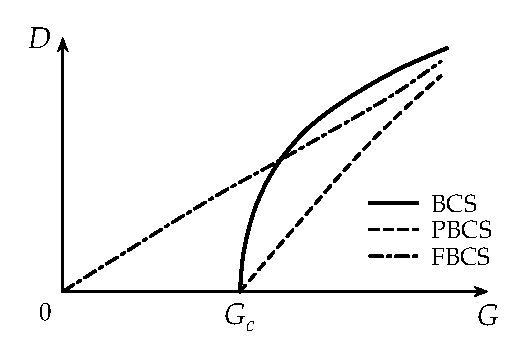
\includegraphics[width=0.55\linewidth]{pictures/11_5}
\par\end{centering}
\centering{}\caption{\label{fig:11_5}BCS（实线）、PBCS（虚线）和FBCS（点虚线）方法中配对关联作为耦合强度 $G$ 的函数（定性）。}
\end{figure}

正如我们在7.7节中所看到的，在这些情况下，我们需要完整的HFB理论，也就是说，我们还必须相对于单粒子波函数 ${\varphi}_{k}$
进行变分。变分后的粒子数投影HFB理论可以通过到目前为止讨论的方法相当简单地得到。由于规范基中的一般HFB波函数（见7.2节）具有BCS函数的结构，我们只需转换到规范基并以相同的方式获得投影矩阵元。

一种避免这些变换的近似方法是基于Fomenko的想法，即将式（11.66）中的积分替换为单位圆上 $L$ 个点 ${\zeta}_{l}=\exp\left({{2\pi il}/L}\right)$
的求和{[}Fo 70, So 72{]}。然后，近似投影算子具有以下形式

\[
{\widehat{P}}^{A}_{L}=\frac{1}{L}\mathop{\sum}\limits^{L}_{{l=1}}{\left({\zeta}_{l}\right)}^{\left({\widehat{N}-A}\right)/2}.\tag{11.74}
\]

很容易看出，除非 $m=0,\pm L,\pm2L,\ldots$，否则 $\widehat{P}^{A+2m}\cdot\widehat{P}^{A}_{L}|\mathrm{BCS}\rangle$
为零。这意味着波函数 $\widehat{P}^{A}_{L}|\mathrm{BCS}\rangle$ 仅包含粒子数 $A,A\pm2L,A\pm4L,\ldots$
的分量。例如，近似投影算符 ${\widehat{P}}^{A}_{2}$ 已经消除了具有 $A\pm2,A\pm6,A\pm{10},\ldots$
的分量。投影后的波函数 $\left({A={2p}}\right)$

\[
{\widehat{P}}^{2p}_{L}|\mathrm{BCS}\rangle=\frac{1}{L}\mathop{\sum}\limits^{L}_{l=1}\zeta^{-p}_{l}\mathop{\prod}\limits_{k>0}\left(u_{k}+v_{k}\zeta_{l}a^{\dagger}_{k}a^{\dagger}_{\bar{k}}\right)|-\rangle\tag{11.75}
\]

是 $L$ 个BCS波函数在规范空间中转动角度 ${\varphi}_{l}={2\pi l}/L$ 后的线性组合；也就是说，
${v}_{k}$ 被替换为 ${e}^{i{\varphi}_{l}}\cdot{v}_{k}$ 。同样， ${\widehat{P}}^{A}_{L}$
将由系数 $\left({{U}_{k{k}^{\prime}},{V}_{k{k}^{\prime}}}\right)$ 给出的HFB函数
$|\Phi\rangle$ 变换为具有系数 $\left({{U}_{k{k}^{\prime}},{\zeta}_{l}{V}_{k{k}^{\prime}}}\right)$
的HFB函数 $\left|{\Phi}_{l}\right\rangle \left({l=1,\ldots,L}\right)$
的线性组合。不需要转换到规范基。

由于BCS波函数仅在少数粒子数上弥散，对于 $L$ 的小值，我们已经得到了近乎精确的投影。

到目前为止，尚未进行粒子数投影后变分的完整HFB理论。无论如何，它比FBCS要复杂得多。在所有实际计算中，使用了依赖于有限数量参数的函数
$|\Phi\left({\beta,\gamma,\Delta}\right)\rangle$ 来最小化投影能量。

\subsection{大形变情况下的近似投影}

Kamlah \cite{Ka68}针对转动群的情况给出了一种在强对称性破缺情况下近似投影的非常通用的方法（另见\cite{Ku72}）。由于转动群表现出许多复杂的特殊特征，并且由于该方法也适用于其他情况，例如粒子数{[}DMR
75, Ma 75a{]}，我们将在此仅针对围绕固定轴的一维转动情况进行介绍。它将由算符 $\widehat{\boldsymbol{J}}$
和角度 $\alpha$ 描述。

投影到 $\widehat{\boldsymbol{J}}$ 的本征函数上的投影算符具有形式（11.57）

\[
{\widehat{P}}^{I}=\frac{1}{2\pi}{\int}^{2\pi}_{0}{e}^{{\mathrm{i}\alpha}\left({\widehat{j}-I}\right)}{\,\mathrm{d}\alpha}\tag{11.76}
\]

对于投影能量，我们得到

\[
{E}^{I}_{\text{ proj }}=\frac{\left\langle \Phi\left|H{\widehat{P}}^{I}\right|\Phi\right\rangle }{\left\langle \Phi\left|{\widehat{P}}^{I}\right|\Phi\right\rangle }=\frac{\int{\,\mathrm{d}\alpha h}\left(\alpha\right){e}^{-{\mathrm{i}I\alpha}}}{\int{\,\mathrm{d}\alpha n}\left(\alpha\right){e}^{-{\mathrm{i}I\alpha}}}\tag{11.77}
\]

带有重叠积分

\[
\left\{ \begin{matrix}h\left(\alpha\right)\\
n\left(\alpha\right)
\end{matrix}\right\} =\langle\Phi\left|{\left\{ \begin{matrix}H\\
1
\end{matrix}\right\} {e}^{{\mathrm{i}\alpha}\widehat{J}}}\right|\Phi\rangle.\tag{11.78}
\]

在粒子数多且变形大的情况下，我们期望函数 $n\left(\alpha\right)$ 和 $h\left(\alpha\right)$
在 $\alpha=0$ 处尖锐地峰值化，而在其他地方消失，使得商 $h\left(\alpha\right)/n\left(\alpha\right)$
是一个相当平滑的函数。这是多体波函数的一个普遍性质（在第10.7节中进行了详细讨论）。遵循第10.7.4节的论证，我们得到\footnote{在以下内容中，我们使用符号 $|\rangle$ 表示归一化的内禀函数 $|\Phi\rangle$。}

\[
n(\alpha)\simeq\exp\left(\mathrm{i}\langle\hat{\boldsymbol{J}}\rangle\cdot\boldsymbol{\alpha}-\frac{1}{2}\langle\Delta\hat{\boldsymbol{J}}^{2}\rangle\alpha^{2}\right),\tag{11.79}
\]

其中

\[
\Delta\widehat{J}=\widehat{J}-\langle\widehat{J}\rangle,
\]

现在唯一的区别是我们也允许波函数中有时间奇数分量，这不会给出纯Gauss分布，而是在式（11.79） $\left({\langle\widehat{J}\rangle\neq0}\right)$
中有一个附加相位。Kamlah的想法是现在使用算符

\[
\widehat{I}\mathrel{\text{ := }}-\langle\widehat{J}\rangle+\frac{1}{i}\frac{\partial}{\partial\alpha},
\]

它是参数 $\alpha$\footnote{对于三维转动的情形，我们因此使用 Euler 角中的角动量表示（见附录 A）来代替 $(1/\mathrm{i})\partial/\partial\alpha$。}
空间中对称算符的一种表示，并以下列方式展开Hamilton重叠函数 $h\left(\alpha\right)$ 。

\[
h\left(\alpha\right)=\mathop{\sum}\limits^{M}_{{n=0}}{h}_{n}{\widehat{I}}^{n}n\left(\alpha\right).\tag{11.80}
\]

从数学上讲，这本质上对应于Fourier变换函数 $h\left(\alpha\right)/n\left(\alpha\right)$
的Taylor展开。由于我们只需要在 $\alpha=0$ 附近的 $h\left(\alpha\right)$ ，如果适当调整，我们已经可以希望用几个非零常数
${h}_{0},{h}_{1},\ldots,{h}_{M}$ 对这个函数得到一个非常好的近似。数字 $M$ 当然取决于重叠（11.79）的宽度，即取决于对称算符
$\widehat{J}$ 在波函数 $|\Phi\rangle$ 中的涨落 $\left\langle {\Delta{\widehat{J}}^{2}}\right\rangle $
。对称性破缺越大，对于低 $M$ 值，近似就越好。

展开式（11.80）不是微扰展开，即系数 ${h}_{n}$ 不是一个接一个地逐步确定，使得系数 ${h}_{0}$ 从 $M$
到 $M+1$ 不会改变，而是对于每个 $M$ 值，整个集合 ${h}_{0},\ldots,{h}_{M}$ 会一次性计算出来：用
$1,\widehat{I},{\widehat{I}}^{2},\ldots,{\widehat{I}}^{M}$ 作用于式（11.80），在极限
$\alpha\rightarrow0$ 下，我们得到关于未知数 ${h}_{0},\ldots,{h}_{M}$ 的如下非齐次方程组：

\[
\left\langle {H{\left(\Delta\widehat{J}\right)}^{m}}\right\rangle =\mathop{\sum}\limits^{M}_{{n=0}}{h}_{n}\left\langle {\left(\Delta\widehat{J}\right)}^{m+n}\right\rangle .\tag{11.81}
\]

这些方程的解为我们给出了投影能量的一个表达式。由（11.77）和（11.80），我们得到

\[
{E}^{I}_{\text{ proj }}=\mathop{\sum}\limits^{M}_{{n=0}}{h}_{n}\cdot{\left(I-\langle\widehat{J}\rangle\right)}^{n}.\tag{11.82}
\]

最简单的情况是 $M=1$ 。在这里我们发现

\[
{h}_{0}=\langle H\rangle,\;{h}_{1}=\frac{\langle{H\Delta}\widehat{J}\rangle}{\left\langle \Delta{\widehat{J}}^{2}\right\rangle },\tag{11.83}
\]

和

\[
{E}^{I}_{\text{ proj }}=\left\langle {\Phi\left|{H-{h}_{1}\widehat{J}}\right|\Phi}\right\rangle +{h}_{1}\cdot I.\tag{11.84}
\]

在投影方法之后的一种变分方法中，我们得到变分方程

\[
\frac{\delta}{\delta\Phi}\langle\Phi\left|H\right|\Phi\rangle-{h}_{1}\frac{\delta}{\delta\Phi}\langle\Phi\left|\widehat{J}\right|\Phi\rangle+\left({I-\langle\widehat{J}\rangle}\right)\frac{\delta{h}_{1}}{\delta\Phi}=0.\tag{11.85}
\]

它由推转方程的一个解来满足\footnote{在某些情况下，该解并非对应于极小值，而是对应于平坦的极大值。然而，二阶项（$M=2$）保证了该极大值变为极小值 \cite{BMR70}（另见第
11.4.6 节）。}：

\[
\frac{\delta}{\delta\Phi}\langle\Phi|H|\Phi\rangle-\omega\frac{\delta}{\delta\Phi}\langle\Phi|\hat{J}|\Phi\rangle=0,\tag{11.86}
\]

和

\[
\langle\widehat{J}\rangle=I
\]

如果条件 ${h}_{1}=\omega$ 得到满足。为了证明情况总是如此，我们利用这样一个事实，即对于直积波函数集合中的任意变分
$|{\delta\Phi}\rangle$ ，式（11.86）都必须成立。其中一种变分由 $|\delta\Phi\rangle\propto\Delta\widehat{J}|\Phi\rangle=\widehat{J}^{20}|\Phi\rangle$（在第7章准粒子表象的意义下）给出。因此，我们得到

\[
\langle\Delta\widehat{J}H\rangle-\omega\left\langle {\left(\Delta\widehat{J}\right)}^{2}\right\rangle =0,
\]

这表明式（11.83）中的 $\omega={h}_{1}$ 。

我们现在已经证明了一个显著的结果，即在强对称性破缺的情况下，当 $M=1$ 在展开式（11.80）中是一个足够好的近似时，保持平均对称性的转动模型波函数是投影后变分方程的一个解。这个结果并不详细依赖于重叠函数的结构。只需要它们在原点附近有尖锐的峰值这一事实。

到目前为止，我们仅在一维转动的情况下证明了这一点，但结果（正如我们将在第11.4.4节中看到的）只需稍作修改，也可应用于三维情况。

在这种近似下，投影能量由 ${h}_{0}$ 给出，且等于未投影能量。这证明了转动谱的自洽转动模型计算是合理的（见第 7.7 节）。特别地，对于自洽转动惯量，我们发现

\[
{g}^{-1}_{\mathrm{{sc}}}=\frac{\omega}{\langle\widehat{J}\rangle}=\frac{\langle{H\Delta}\widehat{J}\rangle}{\left\langle {\Delta{\widehat{J}}^{2}}\right\rangle \langle\widehat{J}\rangle}.\tag{11.87}
\]

如8.5.4节所讨论的，在 $\omega=0$ 点它与Thouless和Valatin的点相同。

然而，这个简单的结果仅适用于能量期望值。如果我们想要计算矩和跃迁概率，就必须从内禀转动函数进行显式投影（见第11.4.6.4节）。

在展开式（11.80）中对 $M=1$ 的限制不够好的情况下，我们必须采用更高的 $M$ 值。对于 $M=2$，我们忽略\footnote{$\langle\Delta\hat{J}^{3}\rangle$ 测量了 $|\Phi\rangle$ 中 $I$ 分布的不对称性。在
Gauss 模重叠的情况下，它精确为零。} $\langle\Delta\hat{J}^{3}\rangle$，并得到

\[
{h}_{0}=\langle H\rangle-\frac{\left\langle \Delta{\widehat{J}}^{2}\right\rangle }{2{\mathcal{G}}_{Y}},\;{h}_{1}=\frac{\left\langle H\Delta\widehat{J}\right\rangle }{\left\langle \Delta{\widehat{J}}^{2}\right\rangle }=\frac{\left\langle \widehat{J}\right\rangle }{{\mathcal{G}}_{\mathrm{{sc}}}},\;{h}_{2}=\frac{1}{2{\mathcal{G}}_{Y}},\tag{11.88}
\]

其中

\[
\frac{1}{2{g}_{Y}}=\frac{\left\langle {{H\Delta}{\widehat{J}}^{2}}\right\rangle -\langle H\rangle\left\langle {\Delta{\widehat{J}}^{2}}\right\rangle }{\left\langle {\Delta{\widehat{J}}^{4}}\right\rangle -{\left\langle \Delta{\widehat{J}}^{2}\right\rangle }^{2}}.\tag{11.89}
\]

在Gauss范数（11.79）的情况下，我们有 $\left\langle {\Delta{\widehat{J}}^{4}}\right\rangle =3{\left\langle \Delta{\widehat{J}}^{2}\right\rangle }^{2}$
并发现

\[
{g}^{-1}_{Y}=\frac{\left\langle \left(H-\langle H\rangle\right)\Delta{\widehat{J}}^{2}\right\rangle }{{\left\langle \Delta{\widehat{J}}^{2}\right\rangle }^{2}}.\tag{11.90}
\]

投影后的能量现在具有以下形式：

\[
{E}^{I}_{\text{ proj }}=\langle H\rangle-\frac{\left\langle \Delta{\widehat{J}}^{2}\right\rangle }{2{g}_{Y}}+\frac{\left\langle \widehat{J}\right\rangle }{{g}_{\mathrm{{sc}}}}\left({I-\langle\widehat{J}\rangle}\right)+\frac{1}{2{g}_{Y}}{\left(I-\langle\widehat{J}\rangle\right)}^{2}.\tag{11.91}
\]

让我们首先研究投影前的变分方法，这最初是由Peierls和Yoccoz{[}PY 57, Yo 57{]}提出的。这里，波函数 $|\Phi\rangle$
是通过在无约束条件下最小化 $H$ 得到的。因此，它是时间反演不变的，并且期望值 $\langle\widehat{J}\rangle$
和 $\langle H\widehat{J}\rangle$ 为零。然后，能谱具有以下形式

\[
{E}^{I}_{\text{ proj }}=\left\langle {H-\frac{{\widehat{J}}^{2}}{2{g}_{Y}}}\right\rangle +\frac{{I}^{2}}{2{g}_{Y}}.\tag{11.92}
\]

它是一个一维转子的能谱，其转动惯量为Yoccoz值 $\mathcal{J}_{Y}$ （见第11.4.5节）\footnote{Verhaar \cite{Ve63,Ve64} 也针对偶核和奇核中 $K=0$ 和 $K\neq0$ 带的三维转动详细研究了该方法。因此人们可以推导出式（3.1）中
$B$ 和 $C$ 系数以及退耦参数（3.31）的微观表达式。}。带首能量是通过从 HF 能量 $\langle H\rangle$ 中减去对称破缺波函数中的赝转动能量得到的\footnote{关于此贡献的计算，见 \cite{ZN77,VLS79,ER80}。}。这使得基态能量大幅降低。在形变良好的原子核中，这个项的量级为4
- 6 MeV。我们已经在几个例子中遇到过这个项，例如，在冗余坐标方法（见第11.3.2节）以及RPA方法中对对称破缺处理（第8.4.8节）。

进行投影后的变分，我们必须相对于 $|\Phi\rangle$ 最小化式（11.91）的右侧。在赝能量 $\left\langle {\Delta{\widehat{J}}^{2}}\right\rangle /2{\mathcal{J}}_{Y}$
不太依赖于 $|\Phi\rangle$ 的情况下，我们再次发现转动模型是一个解。稀土区域形变良好的原子核的模型计算\cite{BMR70}表明，这个项确实对能量曲面给出了相当平坦的贡献。

坎拉展开式（11.80）的收敛性取决于重叠函数在原点处的峰值尖锐程度。它由宽度 $\left\langle {\Delta{\widehat{J}}^{2}}\right\rangle $
衡量，也就是由对称算符的涨落衡量。如果这个涨落很大，展开式收敛很快。我们称这种情况为大形变极限，并且我们想要强调这个极限不一定与相应平均场中的大形变参数相关。在粒子数很大的情况下，即使形变参数很小，涨落
$\left\langle {\Delta{\widehat{J}}^{2}}\right\rangle $ 也可能有很大的值。实际上，基态下“形变良好”的重核形状与球体并没有太大差别（例如，见图7.5）。然而，由于粒子数很大，重叠函数在原点处强烈峰值化，这表明向形变平均场的相变假设是合理的。

\subsection{惯性参数}

在所有与连续对称性破缺相关的集体运动中，势能 $\langle H\rangle$ （11.9） 不依赖于集体坐标。因此，不存在恢复力，并且在大多数转动类型的情况下，我们总是得到大振幅的运动。因此，集体Hamilton量的关键参数是惯性参数。

有一种情况我们可以先验地知道这个参数：由于伽利略不变性，平移的集体惯性必须等于系统的总质量 ${Am}$ 。因此，这种情况为迄今为止在处理对称性破缺时使用的不同近似方案提供了一个非常好的检验。

我们从投影后变分法开始{[}Ze 65, Vi 66, RY 66{]}。方程（11.62）定义了具有动量p的波函数的本征解：

\[
\langle{\delta\Phi}\left|{\left({H-{E}^{\boldsymbol{p}}}\right){\widehat{P}}^{\boldsymbol{p}}}\right|\Phi\rangle=0.\tag{11.93}
\]

从实验室系统变换到以速度 $\boldsymbol{v}=\boldsymbol{p}/{2Am}$ 运动的系统，我们发现（ $\boldsymbol{R}$
是质心坐标）：

\[
|\Phi\rangle={e}^{(\mathrm{i}/\hbar)\boldsymbol{p}\cdot\boldsymbol{R}}|{\Phi}^{\prime}\rangle\tag{11.94}
\]

和

\[
\left\langle {\delta{\Phi}^{\prime}\left|{{e}^{-\left({\mathrm{i}/\hbar}\right)\boldsymbol{p}\boldsymbol{R}}\left({H-{E}^{\boldsymbol{p}}}\right){\widehat{P}}^{\boldsymbol{p}}{e}^{\left({\mathrm{i}/\hbar}\right)\boldsymbol{p}\boldsymbol{R}}}\right|{\Phi}^{\prime}}\right\rangle =0.\tag{11.95}
\]

使用投影仪 ${\widehat{P}}^{\mathrm{p}}$ 的定义（11.59），我们得到变换

\[
{e}^{-\left({\mathrm{i}/\hbar}\right)\boldsymbol{p}\boldsymbol{R}}{\widehat{P}}^{\boldsymbol{p}}{e}^{\left({\mathrm{i}/\hbar}\right)\boldsymbol{p}\boldsymbol{R}}={\widehat{P}}^{\boldsymbol{0}}.\tag{11.96}
\]

对于局部两体相互作用，我们得到

\[
{e}^{-\left({\mathrm{i}/\hbar}\right)\boldsymbol{p}\boldsymbol{R}}H{e}^{\left({\mathrm{i}/\hbar}\right)\boldsymbol{p}\boldsymbol{R}}=H+\frac{\boldsymbol{{pP}}}{Am}+\frac{{\boldsymbol{p}}^{2}}{2Am}.\tag{11.97}
\]

由于 ${\widehat{P}}^{0}$ 投影到质心动量 $\boldsymbol{P}$ 的本征值为零的态上，式（11.95）具有如下形式

\[
\left\langle {\delta{\Phi}^{\prime}\left|{\left({H-{E}^{\mathrm{p}}+\frac{{\boldsymbol{p}}^{2}}{2Am}}\right){\widehat{P}}^{0}}\right|{\Phi}^{\prime}}\right\rangle =0.\tag{11.98}
\]

它对应于动量和能量 ${E}^{0}$ 消失时的变分问题。因此，具有动量 $\boldsymbol{p}$ 的系统的能量由下式给出

\[
{E}^{\mathrm{p}}={E}^{0}+\frac{{\boldsymbol{p}}^{2}}{2Am},\tag{11.99}
\]

这表明我们在变分后使用投影方法获得了正确的总质量。如果我们通过自洽转动模型\cite{Gr60}（在平移的情况下，我们通常说“推”模型）来近似变分后的投影，这个性质是守恒的：

\[
\langle{\delta\Phi}\left|{H-\boldsymbol{v}\boldsymbol{P}}\right|\Phi\rangle=0.\tag{11.100}
\]

通过这种方式得到的Thouless和Valatin的惯性参数（8.113）就是总质量。原则上，我们在8.4.7节中已经证明了这一点，但如果我们使用允许的变分，很容易再次验证它

\[
|\delta\Phi\rangle\propto\boldsymbol{R}|\Phi\rangle.\tag{11.101}
\]

用式（11.100）的复共轭减去它本身，我们得到

\[
\langle\Phi\left|{\left\lbrack {H,\boldsymbol{R}}\right\rbrack -\boldsymbol{v}\cdot\left\lbrack {\boldsymbol{P},\boldsymbol{R}}\right\rbrack }\right|\Phi\rangle=0.\tag{11.102}
\]

在仅包含局部两体相互作用的 $H$ 情况下，我们得到

\[
\boldsymbol{v}=\frac{\langle\Phi\left|\boldsymbol{P}\right|\Phi\rangle}{Am},\tag{11.103}
\]

这表明，由 $\boldsymbol{P}$ 的期望值与速度 $\boldsymbol{v}$ 的比值给出的惯性参数再次是总质量。

如果我们将Hamilton量 $H$ 中的两体相互作用替换为单体势（在这种情况下变分原理等同于精确对角化），那么我们也可以从变分方程（11.93）推导出简单的Inglis公式{[}见式（3.89）{]}作为惯性参数。这向我们表明，对于局部单体势，例如对于
Woods-Saxon 势阱，Inglis 公式也给出了精确的总质量\footnote{这与 Thouless-Valatin 质量（8.113）由于剩余相互作用而与 Inglis 公式不同的事实并不矛盾，因为对于产生局域
HF 场的所有力，剩余相互作用对质量没有影响（式（12.81）中的时间奇部分 $\Gamma_{1}$ 消失）。} \cite{Vi63}。

投影前变分法的一个缺点是它违反了伽利略不变性，该方法得出了Yoccoz\footnote{内禀波函数 $|\Phi\rangle$ 是转动带所有成员 $\Psi^{I}$ 的叠加这一思想也被 Skyrme \cite{Sk57}
使用过：假设内禀 Hamilton 量 $H'=H-\boldsymbol{J}^{2}/2\mathcal{J}$ 具有一个本征态，该本征态不是
$\boldsymbol{J}^{2}$ 的本征态，我们可以证明 \cite{Li60a} $H$ 具有以 $\mathcal{J}$
为转动惯量的转动能谱。为了确定 $\mathcal{J}$ 的最优值，Skyrme 针对参数 $\mathcal{J}$ 最小化期望值
$\langle(H'-\langle H'\rangle)^{2}\rangle$，并找到如下解：
\[
\frac{1}{2\mathcal{J}_{\text{Skyrme}}}=\frac{\langle(H-\langle H\rangle)\boldsymbol{J}^{2}\rangle}{\langle\boldsymbol{J}^{4}\rangle-\langle\boldsymbol{J}^{2}\rangle^{2}}.
\]
对于时间偶波函数，此表达式与式（11.89）完全相同，因此与 $\mathcal{J}_{Y}$ 紧密相关（另见 \cite{Wo75}）。} 的惯性（11.90）。它不能产生精确的质量。从方程（11.90）和（10.134）中，我们用8.4.7节的符号表示法得到惯性（另见\cite{FW70}）：

\[
{g}^{-1}_{Y}=\frac{1}{4{\left\langle \Delta{P}^{2}\right\rangle }^{2}}{\left\langle {\left\lbrack P,{\left\lbrack H,P\right\rbrack }_{+}\right\rbrack }_{+}\right\rangle }_{L}=\frac{\left({{P}^{*}P}\right)\left(\begin{matrix}A & B\\
{B}^{*} & {A}^{*}
\end{matrix}\right)\left(\begin{matrix}P\\
{P}^{*}
\end{matrix}\right)}{{\left(2\mathop{\sum}\limits_{{mi}}{\left|{P}_{mi}\right|}^{2}\right)}^{2}},\tag{11.104}
\]

其中，如果使用自洽基 $\left({{H}^{20}=0}\right)$ ，则 $P$ 是矢量 $\boldsymbol{P}$
的一个分量的 ${ph}$ 部分。在残余相互作用消失的极限情况下，它等于

\[
{\mathcal{I}}_{Y}\left({V=0}\right)=\frac{2{\left(\mathop{\sum}\limits_{{mi}}{\left|{P}_{mi}\right|}^{2}\right)}^{2}}{\mathop{\sum}\limits_{{mi}}{\left|{P}_{mi}\right|}^{2}\left({{\epsilon}_{m}-{\epsilon}_{i}}\right)}.\tag{11.105}
\]

它显然与 Thouless - Valatin 惯性（8.108）不同，

\[
{g}^{-1}_{\mathrm{{TV}}}=\frac{1}{{\hbar}^{2}}\left\langle {\left\lbrack R,{\left\lbrack H,R\right\rbrack }_{-}\right\rbrack }_{-}\right\rangle =\frac{2}{{\hbar}^{2}}{S}_{1}\left(R\right)
\]

or

\[
{g}_{\mathrm{{TV}}}=\frac{1}{2}\left({{P}^{*}P}\right){\left(\begin{array}{ll}
A & B\\
{B}^{*} & {A}^{*}
\end{array}\right)}^{-1}\left(\begin{array}{l}
P\\
{P}^{*}
\end{array}\right)\tag{11.106}
\]

在相互作用消失的极限情况下，它会过渡到 Inglis 公式（3.89），

\[
\mathcal{J}^{-1}_{\text{TV}}(V=0)=2\sum_{mi}\frac{|P_{mi}|^{2}}{\epsilon_{m}-\epsilon_{i}}.\tag{11.107}
\]

这种差异实际上有多大以及有多重要，尚未得到充分研究。它肯定取决于相互作用和单粒子能量 ${\epsilon}_{k}$ 。对于所有具有恒定能级间距
$\epsilon={\epsilon}_{m}-{\epsilon}_{i}$ 的模型，这两个值是相同的。在第 10.7 节中我们看到，如果我们使用具有坐标依赖生成函数的简单
GCM 方法，对于各种集体运动我们都有 Yoccoz 惯性（11.104）。只有在我们允许本征函数 $|\Phi\rangle$
也具有依赖于动量的时间奇数分量的理论中，我们最终才能得到正确的质量。在含时 Hartree - Fock 方法（见第 12 章）和投影后变分方法中就是这种情况。

为了在 GCM 方法中也得到正确的质量，Thouless 和 Peierls \cite{PT62} 提议不仅叠加不同位置的波函数
{[}见式（11.59）{]}，

\[
|\Phi(\boldsymbol{q})\rangle={e}^{(\mathrm{i}/\hbar)\boldsymbol{q}\cdot\boldsymbol{P}}|\Phi\rangle,\tag{11.108}
\]

而且叠加不同速度的波函数，

\[
|\Phi(\boldsymbol{q},\boldsymbol{v})\rangle=e^{-(\mathrm{i}/\hbar)M\boldsymbol{v}\cdot\boldsymbol{R}}|\Phi(\boldsymbol{q})\rangle.\tag{11.109}
\]

这产生了一种双投影方法，其中权重函数 $f\left({\boldsymbol{q},\boldsymbol{v}}\right)$
的速度依赖性必须通过变分来确定。我们可以证明以这种方式得到的波函数不违反伽利略不变性。然而，该方法本身相当复杂，到目前为止尚未得到广泛应用
\cite{Ba69b}。在实际计算中，通常更喜欢投影后变分方法（见第 11.4.2 节）。

到目前为止，我们只处理了平移的情况。在第 10.7 节中讨论的转动或其他集体运动的情况下，情况更为复杂。精确的转动惯量事先并不知道。我们只能类比平移的情况进行论证。数值计算至少表明，在转动情况下，通过
Thouless 和 Valatin 方法得到的转动惯量，在适当处理配对关联的情况下，与实验数据吻合得很好（见图 3.14）。

\subsection{角动量投影}

\subsubsection{类投影算符的推导}

转动群通常由三个 Euler 角\footnote{也使用过其他表示，例如对于参数为 $\varphi_{x},\varphi_{y},\varphi_{z}$ 的一般转动使用 $R=\exp(\mathrm{i}\boldsymbol{\varphi}\cdot\hat{\boldsymbol{J}})$
\cite{KO77}。} $\Omega=\left({\alpha,\beta,\gamma}\right)$ 参数化，一般转动由式（A.4）给出。我们必须回到波函数
$|\Psi\rangle$ 的假设式（11.53）。如同式（11.55），我们将权重函数 $f\left(\Omega\right)$
展开为相应对称算符的一组完备本征函数：用Euler角表示的角动量。如附录A中所讨论的，这样一组函数由Wigner函数 ${D}^{{I}^{*}}_{MK}\left(\Omega\right)$
给出。因此我们得到假设式

\[
f\left(\Omega\right)=\frac{{2I}+1}{8{\pi}^{2}}\mathop{\sum}\limits_{{IMK}}{g}_{IMK}{D}^{{I}^{*}}_{MK}\left(\Omega\right)\tag{11.110}
\]

以及

\[
|\Psi\rangle=\mathop{\sum}\limits_{IMK}g_{IMK}\widehat{P}^{I}_{MK}|\Phi\rangle.\tag{11.111}
\]

算符{[}RW 54, PY 57, Vi 66{]}

\[
{\widehat{P}}^{I}_{MK}=\frac{{2I}+1}{8{\pi}^{2}}\int{D}^{{I}^{*}}_{MK}\left(\Omega\right)R\left(\Omega\right){\,\mathrm{d}\Omega}\tag{11.112}
\]

\[
R\left(\Omega\right)={e}^{{\mathrm{i}\alpha}{\widehat{J}}_{z}}{e}^{{\mathrm{i}\beta}{\widehat{J}}_{y}}{e}^{{\mathrm{i}\gamma}{\widehat{J}}_{z}}
\]

可以类似于式（11.58）那样书写{[}LB 68, Co 71{]}

\[
\widehat{P}^{I}_{MK}=\mathop{\sum}\limits_{\alpha}|IM\alpha\rangle\langle IK\alpha|,\tag{11.113}
\]

其中 $|{IM\alpha}\rangle$ 是希尔伯特空间中的一组完备正交归一化函数集， $\alpha$ 除了转动量子数
$I$ 和 $M$ 之外还表征所有量子数。

从式（11.113）我们看到 ${\widehat{P}}^{I}_{MK}$ 在数学意义上不是投影算符。我们只有以下关系

\[
{\widehat{P}}^{I}_{MK}{\widehat{P}}^{{I}^{\prime}}_{{M}^{\prime}{K}^{\prime}}={\delta}_{I{I}^{\prime}}{\delta}_{{M}^{\prime}K}{\widehat{P}}^{I}_{M{K}^{\prime}};\;\left({\widehat{P}}^{I}_{MK}\right)^{\dagger}={\widehat{P}}^{I}_{KM}.\tag{11.114}
\]

为了展示它们如何相对于具有量子数 $K$ 的算符 ${\widehat{J}}_{z}$ 的本征态作用于“内秉”\footnote{实际上，在 GCM 方法中我们既不引入内秉参考系也不引入冗余坐标。“内秉”波函数 $|\Phi\rangle$ 与实验室参考系中的函数
$|\Psi\rangle$ 之间的联系不是由坐标变换给出，而是由 GCM 假设式（11.111）给出。}违反对称性的波函数$|\Phi\rangle$，我们将 $|\Phi\rangle$ 分解为：

\[
|\Phi\rangle=\mathop{\sum}\limits_{K'}|\Phi_{K'}\rangle;\quad\widehat{J}_{z}|\Phi_{K}\rangle=K|\Phi_{K}\rangle.\tag{11.115}
\]

${\widehat{P}}^{I}_{MK}$ 将分量 $\left|{\Phi}_{K}\right\rangle $ 变换为具有量子数
$I$ 和 $M$ 的 ${\widehat{\boldsymbol{J}}}^{2}$ 和 ${\widehat{J}}_{z}$
的本征函数，并使所有其他具有 ${K}^{\prime}\neq K$ 的分量湮灭。

原则上，构造到量子数 $I,M$ 上的精确数学投影算符非常简单。它由\footnote{这个算符已由 Löwdin \cite{Lo64} 以如下方式表示：
\[
\hat{P}^{I}_{MM}=\prod_{L\neq I}\frac{\hat{\boldsymbol{J}}^{2}-L(L+1)}{I(I+1)-L(L+1)}\prod_{K\neq M}\frac{\hat{J}_{z}-K}{M-K}.
\]
在这个算符的实际应用中，我们最终得到一组代数方程（另见 \cite{KL64,Ke66,Ul71,Ul72,MKL71,MM76}），并且不必对
Euler 角进行积分。}给出

\[
\widehat{P}^{I}_{MM}=\mathop{\sum}\limits_{\alpha}|IM\alpha\rangle\langle IM\alpha|.\tag{11.116}
\]

然而，从式（11.115）我们看到这个算符相当不物理。例如，作用于具有 $K=0$ 的轴对称Nilsson函数上，我们只会得到具有
$M=0$ 的波函数 $\left|{\Psi}^{IM}\right\rangle $ ，这显然违反了转动对称性。

因此我们必须使用一般拟设\footnote{正如我们从式（11.120）中看到的，系数 $g_{K}$ 当然也依赖于 $I$。然而，我们省略了指标 $I$。}

\[
|\Psi^{IM}\rangle=\mathop{\sum}\limits_{K}g_{K}\widehat{P}^{I}_{MK}|\Phi\rangle=\mathop{\sum}\limits_{K}g_{K}\frac{2I+1}{8\pi^{2}}\int\,\mathrm{d}\Omega\,D^{I*}_{MK}(\Omega)R(\Omega)|\Phi\rangle.\tag{11.117}
\]

在波函数 $|\Phi\rangle$ 具有轴对称性的情况下，只有 $K$ 值 ${K}_{0}$ 对总和（11.117）有贡献，并且系数
${g}_{{K}_{0}}$ 由归一化给出。然而，一般来说，我们必须相对于系数 ${g}_{K}$ 使Hamilton量最小化。能量由下式给出

\[
{E}^{I}_{\text{ proj }}=\frac{\left\langle {\Psi}^{IM}\left|H\right|{\Psi}^{IM}\right\rangle }{\left\langle {\Psi}^{IM}\mid{\Psi}^{IM}\right\rangle }=\frac{\mathop{\sum}\limits_{{K{K}^{\prime}}}{g}^{*}_{K}{g}_{{K}^{\prime}}{h}^{I}_{K{K}^{\prime}}}{\mathop{\sum}\limits_{{K{K}^{\prime}}}{g}^{*}_{K}{g}_{{K}^{\prime}}{n}^{I}_{K{K}^{\prime}}},\tag{11.118}
\]

以及核

\[
h^{I}_{KK'}=\langle\Phi|H\hat{P}^{I}_{KK'}|\Phi\rangle,
\]

\[
n^{I}_{KK'}=\langle\Phi|\hat{P}^{I}_{KK'}|\Phi\rangle.\tag{11.119}
\]

系数 ${g}_{K}$ 是广义特征值问题的解

\[
\mathop{\sum}\limits_{{K}^{\prime}}{h}^{I}_{K{K}^{\prime}}{g}_{{K}^{\prime}}={E}^{I}\mathop{\sum}\limits_{{K}^{\prime}}{n}^{I}_{K{K}^{\prime}}{g}_{{K}^{\prime}}.\tag{11.120}
\]

它对应于Hamilton量 $H$ 在由非正交系统 ${\widehat{P}}^{I}_{MK}|\Phi\rangle$ 所张成空间中的对角化。

在第10.7节中，我们看到了如何进行操作以便最终得到一个厄米特特征值问题。我们必须要么将集合 ${\widehat{P}}^{I}_{MK}|\Phi\rangle$
正交化，要么计算矩阵 ${n}^{I}_{K{K}^{\prime}}$ 的平方根。在重叠函数 $\langle\Phi\left|{R\left(\Omega\right)}\right|\Phi\rangle$
为Gauss形式的情况下，也就是说，对于一个强变形波函数（见第11.4.4节），我们可以解析地做到这一点。由于我们面临的是一个三维问题，最终会得到一个像式（10.145）那样的集体Hamilton量。Une等人\cite{UIO76}已经表明，它具有转子Hamilton量（1.55）的精确形式，其转动惯量由Yoccoz公式\footnote{另见 \cite{ABC77a}。}
给出（见第11.4.5节）。

如果我们定义极其变形的多体波函数\footnote{这些函数对应于式（10.20）及后续讨论的双正交基。}
$|\Omega\rangle$ ，它在方向 $\Omega$ 上像针一样指向，那么与集体转子模型的紧密类比就很容易可视化。它们在
$\Omega$ 空间中几乎是局域化的。这些函数与波函数 $\left|{\Psi}^{IM}\right\rangle $ （11.117）之间的重叠

\[
\langle\Omega|{\Psi}^{IM}\rangle\propto\mathop{\sum}\limits_{K}\;{g}_{K}\int d{\Omega}^{\prime}\;{D}^{{I}^{*}}_{MK}\left({\Omega}^{\prime}\right)\langle\Omega|R\left({\Omega}^{\prime}\right)|\Phi\rangle,\tag{11.121}
\]

测量在角度 $\Omega$ 处找到系统的概率幅。在波函数 $|\Phi\rangle$ 充分变形且在 $\Omega=0$
处达到峰值的极限情况下，重叠 $\left\langle {\Omega\left|{R\left({\Omega}^{\prime}\right)}\right|\Phi}\right\rangle $
在 $\Omega$ 空间中的行为类似于 $\delta$ 函数 $\delta\left({\Omega-{\Omega}^{\prime}}\right)$
，并且我们得到{[}Ze 67, FJM 71{]}

\[
\langle\Omega|\Psi^{IM}\rangle\propto\sum_{K}g_{K}D^{I*}_{MK}(\Omega)\tag{11.122}
\]
\footnote{【译者注】也使用过其他表示，例如 $R=\mathrm{e}^{-\mathrm{i}\alpha J_{z}}\mathrm{e}^{-\mathrm{i}\beta J_{y}}\mathrm{e}^{-\mathrm{i}\gamma J_{z}}$
；此时 $D$ 函数与 Edmonds \cite{Ed57} 的相符合。我们在这里使用的定义（11.118）与 Rose \cite{Ro57}
的相符合。}

这正是一个转子的波函数（见第1.5.1节）。在这种近似下，变形函数 $|\Phi\rangle$ 在空间中像转子一样运动。然而，我们必须强调，我们没有使用冗余变量。Euler角
$\Omega$ 仅仅是用作生成坐标的参数。

与转子的对称行为类似，在群 ${D}_{2}$ 的某些操作下{[}例如，式（1.57）及后续中的 ${\Re}_{1}$ 或 ${\Re}_{2}$
{]}会导致展开系数 ${g}^{\left(\text{ rotor }\right)}_{K}$ 之间的关系，现在如果我们的内部波函数具有这些对称性，我们就可以为系数
${g}_{K}$ 推导相应的关系。

作为一个例子，我们使用 ${180}^{\circ}$ 绕 $x$ 轴的转动。我们假设\footnote{这一假设与我们方法的转动不变性是相容的，因为内部波函数 $|\Phi\rangle$ 绕 Euler 角 $\Omega$ 的转动可以表示为系数
$g_{K}$ 的变换，正如我们从关系式
\[
\hat{P}^{I}_{MK}R(\Omega)=\sum_{K'}D^{I}_{KK'}(\Omega)\hat{P}^{I}_{MK'}\tag{11.123}
\]
中所看到的。只要我们考虑任意系数 $g_{K}$，我们就可以自由选择 $|\Phi\rangle$ 的取向。}内部波函数 $|\Phi\rangle$ 关于此操作是一个本征函数：

\[
{e}^{\mathrm{i}\pi{\widehat{J}}_{x}}|\Phi\rangle={r}_{x}|\Phi\rangle.\tag{11.124}
\]

对于粒子数为偶数的系统，本征值 ${r}_{x}$ 为 $\pm1$ ；对于粒子数为奇数的系统，本征值为 $\pm i$ 。它常被称为signature
\cite{Bo76b}。例如，在变形的Nilsson势阱中，偶偶核的基态总是具有 ${r}_{x}=+1$ ，因为以 $\pm i$
成对占据简并能级会给出最低能量。因此，基态带的 ${r}_{x}=+1$ 条件是变分原理的自然结果。这一事实为转子模型的假设（1.58）提供了微观基础——即变形核相对于操作
${\Re}_{1}$ （1.57）具有本征值 +1。

对称性（11.123）相当普遍，也适用于转动模型波函数。到目前为止，尚未发现它无效的实验证据。因此，我们将在以下内容中使用这种对称性。

如果我们像在式（11.115）中那样，将内部波函数 $|\Phi\rangle$ 分解为具有良好 $K$ 量子数的分量 $\left|{\Phi}_{K}\right\rangle $
，那么从（11.123）可得：

\[
{e}^{{\mathrm{i}\pi}{\widehat{J}}_{x}}\left|{\Phi}_{K}\right\rangle ={r}_{x}\left|{\Phi}_{-K}\right\rangle .\tag{11.125}
\]

从式（11.124）我们可以推断出

\[
{\widehat{P}}^{I}_{MK}{e}^{{\mathrm{i}\pi}{\widehat{J}}_{x}}={\left(-\right)}^{I}{\widehat{P}}^{I}_{MK},\tag{11.126}
\]

这表明态

\[
\widehat{P}^{I}_{MK}|\Phi\rangle=\widehat{P}^{I}_{MK}|\Phi_{K}\rangle\quad\text{以及}\quad\widehat{P}^{I}_{M-K}|\Phi\rangle=\widehat{P}^{I}_{M-K}|\Phi_{-K}\rangle
\]

在希尔伯特空间中对应于同一态。因此，我们可以限制式（11.117）中对 $K\geq0$ 的求和。\footnote{【译者注】正如我们从式（11.120）中看到的，系数 $a_{M}$ 仅由实验室系统中的边界条件决定（例如磁量子数 $M$ 
的指定）。对于孤立核，所有 $M$ 
态简并，我们通常只考虑 $a_{M}=\delta_{MM_{0}}$ 的情形。}

表示

\[
\left|{\Psi}^{IM}\right\rangle =\mathop{\sum}\limits_{{K>0}}\frac{{g}_{K}}{1+{\delta}_{K0}}\left({{\widehat{P}}^{I}_{MK}+{\left(-\right)}^{I}{r}^{-1}_{x}{\widehat{P}}^{I}_{M-K}}\right)|\Phi\rangle\tag{11.127}
\]

清楚地表明，对于奇数 $I$ 值，具有 $K=0$ 和 ${r}_{x}=1$ 的轴对称波函数 $|\Phi\rangle$
投影为零。因此，对于基态带，我们得到自旋序列 $I=0,2,4,\ldots$

在我们只有近似轴对称的情况下，如在转动模型波函数中（见7.7节和11.4.6.3节），剩余的 $K\neq0$ 部分不会投影为零。然而，它们源于两准粒子态和更复杂构型的混合，这些混合处于更高能量，并且仅对本征值问题（11.120）中的高激发能级有贡献，而我们对此并不感兴趣。因此，对于基态带，我们应该施加条件

\[
{r}_{x}={\left(-\right)}^{I}.\tag{11.128}
\]


\subsubsection{双变分法\label{subsec:=0053CC=0053D8=005206=006CD5}}

到目前为止，我们尚未指定确定内禀波函数 $|\Phi\rangle$ 的方法。与11.4.2节中讨论的阿贝尔群的情况一样，我们可以在投影之前或之后进行变分。然而，在没有轴对称的情况下，情况现在更复杂了，因为我们还必须确定系数
${g}_{K}$ 。在VBP方法中，它们必须通过式（11.120）计算。

在VAP方法中，我们现在得到一个类似于系统（10.147） \cite{Ze67}的耦合系统：

\[
\mathop{\sum}\limits_{{K}^{\prime}}{g}_{{K}^{\prime}}\left\langle {\Phi\left|{\left({H-{E}^{I}}\right){\widehat{P}}^{I}_{K{K}^{\prime}}}\right|\Phi}\right\rangle =0
\]

\[
\mathop{\sum}\limits_{{K{K}^{\prime}}}{g}^{*}_{K}{g}_{{K}^{\prime}}\left\langle {{\delta\Phi}\left|{\left({H-{E}^{I}}\right){\widehat{P}}^{I}_{K{K}^{\prime}}}\right|\Phi}\right\rangle =0.\tag{11.129}
\]

第一部分对应于式（11.120）；第二部分是VAP方程（11.62）的推广。原则上，这个系统必须通过迭代求解。

除了系统（11.129）过于复杂以至于无法精确求解这一事实外，在许多情况下它还包含高度的冗余性。为了看到这一点，我们再次使用 $|\Phi\rangle$
分解为各 $K$ 分量的式（11.115）。利用 ${\widehat{P}}^{I}_{MK}$ 使所有 $K\neq{K}^{\prime}$
的 $\left|{\Phi}_{{K}^{\prime}}\right\rangle $ 分量湮灭这一事实，我们得到

\[
\left|{\Psi}^{IM}\right\rangle =\mathop{\sum}\limits_{K}{\widehat{P}}^{I}_{MK}\mathop{\sum}\limits_{{K}^{\prime}}{g}_{{K}^{\prime}}\left|{\Phi}_{{K}^{\prime}}\right\rangle =\mathop{\sum}\limits_{K}{\widehat{P}}^{I}_{MK}|\widetilde{\Phi}\rangle.\tag{11.130}
\]

函数

\[
|\widetilde{\Phi}\rangle=\mathop{\sum}\limits_{K}{g}_{K}|{\Phi}_{K}\rangle\tag{11.131}
\]

一般来说，它将不再是一个直积波函数。然而，在许多情况下，它可以用这种类型的函数来近似\footnote{一个简单的例子是奇核的波函数
\[
|\Phi\rangle=\sum_{K}C_{K}\beta^{\dagger}_{K}|\Phi_{0}\rangle,
\]
其中一个任意强混合的粒子位于具有 $K=0$ 的核心上；另一个例子是仅略微偏离轴对称的波函数 $|\Phi\rangle$。}。在所有这些情况下，如果我们对 $|\Phi\rangle$ 进行一般变化， ${g}_{K}$ 的变化就是多余的。然后我们得到了简单的算符（最初由Kamlah\cite{Ka68}提出）：

\[
{\widehat{P}}^{I}_{M}=\mathop{\sum}\limits_{K}{\widehat{P}}^{I}_{MK}.\tag{11.132}
\]

它具有 ${\widehat{P}}^{2}=\widehat{P}$ 的性质，但不是厄米算符。从函数 $\left|\widetilde{\Phi}\right\rangle $
转动时它不是不变的这个意义上来说，它也违反了转动对称性\cite{So77}。然而，连同 $|\widetilde{\Phi}\rangle$
的完全变化一起，该过程保持转动不变性，因为我们总是能找到 $|\widetilde{\Phi}\rangle$ 处于这样一个取向，使得能量最小。通过对称性论证，由算符
${\widehat{P}}^{I}_{M}$ 确定的量子化轴应该与 $|\widetilde{\Phi}\rangle$ 中质量分布的一个主轴重合。

算符（11.132）消除了波函数 $|\widetilde{\Phi}\rangle$ 中所有不具有该特征的分量

\[
{r}_{x}={\left(-\right)}^{I}.\tag{11.133}
\]

在偶核中，这一事实保证了基态能带中的自旋序列 $I=0,2,4,\ldots$ ，即使它不再是轴对称的。在奇核中，它导致有利能带和不利能带中的
${\Delta I}=2$ 能级序列具有不同的特征（见3.3节）。

\subsubsection{自洽转动模型}

在11.4.4节中，我们提出了一种推导投影能量近似表达式的方法，而没有过多指定内部波函数 $|\Phi\rangle$ 。出于教学目的，在该节中针对一维转子的情况进行了讨论。它也可以应用于三维转动的一般情况{[}Ka
68, BMR 70, Ma 75a{]}。

由于三维情况涉及相当冗长的计算，我们在此仅给出主要结果：在对“内部”波函数 $|\Phi\rangle$ 的以下三个假设下，即：

（i） 强变形 $\left({\left\langle \Phi\right|{\widehat{J}}^{2}_{y}|\Phi\rangle\gg1}\right)$
，

（ii） 确定的特征标（signature）$(e^{\mathrm{i}\pi\widehat{J}_{x}}|\Phi\rangle\propto|\Phi\rangle)$
，

（iii） 对于小的 $I$ 值近似轴对称（即在基态能带 $\left\langle {\Phi\left|{\widehat{J}}^{2}_{z}\right|\Phi}\right\rangle \ll I\left({I+1}\right))$
中），

我们在Kamlah展开式（11.80）中到二阶项得到以下投影能量的表达式\footnote{$\hat{P}^{I}_{M}$ 是式（11.132）中定义的算符，并且波函数 $|\Phi\rangle$ 被替换为一个简单的右矢
$|\rangle$。} \cite{BMR70}：

\[
{E}^{I}_{\text{ proj }}=\frac{\left\langle H{\widehat{P}}^{I}_{M}\right\rangle }{\left\langle {\widehat{P}}^{I}_{M}\right\rangle }=\langle H\rangle-\frac{\left\langle \Delta{\widehat{\boldsymbol{J}}}^{2}\right\rangle }{2{g}_{Y}}+\omega\left({\sqrt{I\left({I+1}\right)-\left\langle {\widehat{J}}^{2}_{z}\right\rangle }-\left\langle {\widehat{J}}_{x}\right\rangle }\right)
\]

\[
+\frac{1}{2{g}_{Y}}{\left(\sqrt{I\left({I+1}\right)-\left\langle {\widehat{J}}^{2}_{z}\right\rangle }-\left\langle {\widehat{J}}_{x}\right\rangle \right)}^{2},\tag{11.134}
\]

其中

\[
\frac{1}{2{g}_{Y}}=\frac{\left\langle \left(H-\langle H\rangle\right)\Delta{\widehat{\boldsymbol{J}}}^{2}\right\rangle }{2\left({{\left\langle \Delta{\widehat{J}}^{2}_{x}\right\rangle }^{2}+{\left\langle {\widehat{J}}^{2}_{y}\right\rangle }^{2}+{\left\langle {\widehat{J}}^{2}_{z}\right\rangle }^{2}}\right)},\;\omega=\frac{\left\langle H\Delta{\widehat{J}}_{x}\right\rangle }{\left\langle \Delta{\widehat{J}}^{2}_{x}\right\rangle }.
\]

这些表达式与式（11.91）非常相似，我们可以得出相同的结论：在能量中消除赝贡献的项 $\left\langle {\Delta{\widehat{\boldsymbol{J}}}^{2}}\right\rangle /2{\mathcal{G}}_{Y}$
在变化中可以忽略的情况下，我们最终得到转动模型

\[
\delta\left\langle {H-\omega{\widehat{J}}_{x}}\right\rangle =0\tag{11.135}
\]

带有辅助条件

\[
\left\langle {\widehat{J}}_{x}\right\rangle =\sqrt{I\left({I+1}\right)-\left\langle {\widehat{J}}^{2}_{z}\right\rangle }.\tag{11.136}
\]

它与通常的约束（7.97）的不同之处在于项 $\left\langle {\widehat{J}}^{2}_{z}\right\rangle $
。在变形良好的核的基态能带中，它不起任何作用：对于小的 $I$ 值，核几乎是具有 $K=0$ 的轴对称的，并且对于大角动量无论如何它都可以忽略。然而，在
$K\neq0$ 能带的转动计算中考虑它是很重要的，特别是在奇 $A$ 核中{[}RMB 74, RM 74{]}。

因此，我们有了对最初由经典论证引入的转动模型（3.4节）的微观推导。转动波函数必须被理解为内部波函数。实验室坐标系中的波函数是通过用算符（11.132）进行角动量投影得到的。这个推导仅基于大粒子数和大形变的假设，这保证了重叠函数
$n\left(\Omega\right)$ 有一个尖锐的峰值。从这个意义上说，它是一个完全量子力学的推导，不依赖于诸如具有 $\left\langle {\Delta{\widehat{\boldsymbol{J}}}^{2}}\right\rangle \ll{I}^{2}$
的大角动量这样的经典论证；相反，该推导基于我们有大的涨落 $\left\langle {\Delta{\widehat{\boldsymbol{J}}}^{2}}\right\rangle \gg1$
（窄重叠）这一事实。这也意味着通过不确定性关系，角度的展宽很小 $\left({\left\langle {\Delta{\Omega}^{2}}\right\rangle \ll1}\right)$
。

在第12章中，我们将用时变波包的形式重新推导这些关系。例如，在平移的情况下，还会发现原子核在空间中相当局域化（$(\langle\Delta\boldsymbol{R}^{2}\rangle)^{1/2}$
远小于核半径，即波包宽度很小）这一物理事实导致动量展宽 $\left\langle {\Delta{\boldsymbol{P}}^{2}}\right\rangle $
很大。因此，自洽转动模型（在这种情况下是推转模型）将被证明是一个很好的近似。

\subsubsection{电磁矩和跃迁概率\label{subsec:=007535=0078C1=0077E9=00548C=008DC3=008FC1=006982=007387}}

在11.4.4节中我们看到，对于计算形变良好的原子核的转动谱，我们不需要显式的角动量投影。转动模型已经提供了一个相当好的近似。对于在转动下不像标量那样变换的算符的矩阵元，情况就不再如此了，例如电磁多极算符
${\widehat{Q}}_{\lambda\mu}$ 。

对于归一化波函数 $\left|{\Psi}^{{I}_{1}{M}_{1}}_{1}\right\rangle $ 和 $\left|{\Psi}^{{I}_{2}{M}_{2}}_{2}\right\rangle $
（类型为（11.117））之间算符 ${\widehat{Q}}_{\lambda\mu}$ 的约化矩阵元，我们得到

\[
\left\langle {{\Psi}^{{I}_{1}}_{1}\begin{Vmatrix}{\widehat{Q}}_{\lambda}\end{Vmatrix}{\Psi}^{{I}_{2}}_{2}}\right\rangle =\mathop{\sum}\limits_{\substack{{{K}_{1}{K}_{2}}\\
{{\bar{K}}_{2}\mu}
}
}{g}^{\left(1\right)*}_{{K}_{1}}{g}^{\left(2\right)}_{{\bar{K}}_{2}}{\left(-\right)}^{{I}_{1}-{K}_{1}}\left(\begin{matrix}{I}_{1} & \lambda & {I}_{2}\\
-{K}_{1} & \mu & {\bar{K}}_{2}
\end{matrix}\right){\left(\left(2{I}_{1}+1\right)\left(2{I}_{2}+1\right)\right)}^{1/2}
\]

\[
\cdot{Q}^{\mathrm{{\mathrm{i}ntr}}}_{\lambda\mu}\left({{K}_{2},{\bar{K}}_{2}}\right)\text{ , }\tag{11.137}
\]

其中

\[
{Q}^{\text{ intr }}_{\lambda\mu}\left({{K}_{2}{\bar{K}}_{2}}\right)={\mathcal{K}}_{1}{\mathcal{K}}_{2}{\left(\left(2{I}_{1}+1\right)\left(2{I}_{2}+1\right)\right)}^{1/2}
\]

\[
\times\frac{1}{8{\pi}^{2}}\int{\,\mathrm{d}\Omega}{D}^{{I}_{3}}_{{\bar{K}}_{2}{K}_{2}}\left(\Omega\right)\left\langle {{\Phi}_{1}\left|{{\widehat{Q}}_{\lambda\mu}R\left(\Omega\right)}\right|{\Phi}_{2}}\right\rangle .\tag{11.138}
\]

因子 ${\mathcal{R}}_{i}$ 是归一化常数（ $i$ 指的是内禀波函数 $\left.\left|{\Phi}_{i}\right\rangle \right)$
）

\[
{\mathcal{R}}^{-2}_{i}=\mathop{\sum}\limits_{{K{K}^{\prime}}}{g}^{*\left(i\right)}_{K}{g}^{\left(i\right)}_{{K}^{\prime}}{n}^{{I}_{i}\left(i\right)}_{K{K}^{\prime}}.\tag{11.139}
\]

为了计算重叠积分 $\left\langle {{\Phi}_{1}\left|{{\widehat{Q}}_{\lambda\mu}R\left(\Omega\right)}\right|{\Phi}_{2}}\right\rangle $
，我们可以再次使用一种类似Kamlah展开式（11.80），并在零阶得到

\[
\left\langle {{\Phi}_{1}\left|{{\widehat{Q}}_{\lambda\mu}R\left(\Omega\right)}\right|{\Phi}_{2}}\right\rangle =\left\langle {{\Phi}_{1}\left|{\widehat{Q}}_{\lambda\mu}\right|{\Phi}_{2}}\right\rangle \left\langle {{\Phi}_{2}\left|{R\left(\Omega\right)}\right|{\Phi}_{2}}\right\rangle .\tag{11.140}
\]

使用这个近似，我们得到

\[
{Q}^{\mathrm{{\mathrm{i}ntr}}}_{\lambda\mu}\left({{K}_{2}{\bar{K}}_{2}}\right)\propto\left\langle {{\Phi}_{1}\left|{\widehat{Q}}_{\lambda\mu}\right|{\Phi}_{2}}\right\rangle \int{\,\mathrm{d}\Omega}{D}^{{I}_{3}}_{{K}_{2}{K}_{2}}\left(\Omega\right){n}_{2}\left(\Omega\right).\tag{11.141}
\]

其余的积分必须明确计算。只有在非常大的形变极限下，我们才得到{[}Vi 66, Ze 67{]}

\[
{Q}^{\text{ intr }}_{\lambda\mu}\left({{K}_{2}{\bar{K}}_{2}}\right)=\left\langle {{\Phi}_{1}\left|{\widehat{Q}}_{\lambda\mu}\right|{\Phi}_{2}}\right\rangle {\delta}_{{K}_{2}{\bar{K}}_{2}}\tag{11.142}
\]

以及

\[
\left\langle {{\Psi}^{{I}_{1}}_{1}\begin{Vmatrix}{\widehat{Q}}_{\lambda}\end{Vmatrix}{\Psi}^{{I}_{2}}_{2}}\right\rangle =\mathop{\sum}\limits_{{{K}_{1}{K}_{2}\mu}}{g}^{\left(1\right)*}_{{K}_{1}}{g}^{\left(2\right)}_{{K}_{2}}{\left(\left(2{I}_{1}+1\right)\left(2{I}_{2}+1\right)\right)}^{1/2}{\left(-\right)}^{{I}_{1}-{K}_{1}}\left(\begin{matrix}{I}_{1} & \lambda & {I}_{2}\\
-{K}_{1} & \mu & {K}_{2}
\end{matrix}\right)
\]

\[
\times\left\langle {{\Phi}_{1}\left|{\widehat{Q}}_{\lambda\mu}\right|{\Phi}_{2}}\right\rangle \tag{11.143}
\]

一个与集体模型中的式（1.70）相对应的结果。唯一的区别是现在内禀多极矩可以从微观上计算。特别地，我们通过重叠积分 $\left\langle {{\Phi}_{1}\left|{\widehat{Q}}_{\lambda\mu}\right|{\Phi}_{2}}\right\rangle $
考虑内禀波函数 $\left|{\Phi}_{1}\right\rangle $ 和 $\left|{\Phi}_{2}\right\rangle $
之间的差异。

在这种首次近似不够好的情况下，我们需要三维情形下范数重叠 $n\left(\Omega\right)$ 的显式表达式。它可以展开为
\cite{IMR79}

\[
n\left(\Omega\right)=\exp\left({\mathop{\sum}\limits_{{{LK}{K}^{\prime}}}{C}^{L}_{K{K}^{\prime}}{D}^{{L}^{*}}_{K{K}^{\prime}}\left(\Omega\right)}\right).\tag{11.144}
\]

Gauss近似对应于对 $L\leq2$ 的一种限制。类似于式（11.79），我们可以通过 $\left\langle {\widehat{J}}_{i}\right\rangle $
和 $\left\langle {{\widehat{J}}_{i}{\widehat{J}}_{k}}\right\rangle $
的期望值来表示系数 ${C}^{L}_{K{K}^{\prime}}$ 。利用关系式（A.17），对于大形变和小的 $K$ 混合情形{[}BMR
70, VS 71{]}，我们得到

\[
n(\Omega)\simeq\exp\left\{ -\frac{\langle\hat{\boldsymbol{J}}^{2}_{y}\rangle}{2}\beta^{2}+(\cos(\alpha+\gamma)-1)\langle\hat{\boldsymbol{J}}^{2}_{z}\rangle+\frac{\mathrm{i}}{2}\langle\hat{\boldsymbol{J}}_{x}\rangle\beta(\sin\alpha-\sin\gamma)\right\} .\tag{11.145}
\]


\subsubsection{精确角动量投影}

使用精确角动量投影波函数进行计算通常需要大量的数值计算。每个算符的期望值——例如Hamilton量——包含一系列三维积分的求和{[}见式（11.118）和（11.119）{]}。被积函数与重叠函数
$\langle\Phi\left|{R\left(\Omega\right)}\right|\Phi\rangle$ 和 $\langle\Phi\left|{{HR}\left(\Omega\right)}\right|\Phi\rangle$
成正比，必须使用Onishi公式（E.49）逐点计算。只有在轴对称内秉波函数（量子数为 $K$ ）的情形下， $\alpha$
和 $\gamma$ 的依赖关系才变得简单，最终得到一个一维积分：

\[
\left\langle {{\Psi}^{IM}\left|H\right|{\Psi}^{IM}}\right\rangle =\frac{\int\,\mathrm{d}\cos\beta{d}^{I}_{KK}\left(\beta\right)\left\langle {\Phi\left|{{e}^{{\mathrm{i}\beta}{\widehat{J}}_{y}}H}\right|\Phi}\right\rangle }{\int\,\mathrm{d}\cos\beta{d}^{I}_{KK}\left(\beta\right)\left\langle {\Phi\left|{e}^{{\mathrm{i}\beta}{\widehat{J}}_{y}}\right|\Phi}\right\rangle }.
\]

以这种形式，变分前后的角动量投影在文献中经常被应用（综述见{[}Ri 68, Ma 70, Wo 75{]}）。许多研究是在 ${1p}$
和 ${2s}-{1d}$ 壳层内进行的，在那里我们有具有转动特征谱的变形核\cite{BBC72}。在元素周期表的这个区域，角动量投影的HF理论可以与精确壳模型计算{[}Re
58, KP 59, Wa 70b, MMW 73{]}进行比较，并且在许多情况下我们发现完全一致。详细地说，投影HF理论在这些轻核中有许多版本的应用。在最简单的情形下，人们常常在变分后（见11.4.2节）从轴对称变形直积态进行投影{[}KL
64, BGR 65, WG 67b, GFW 72{]}。通过使用依赖于几个变量的内秉波函数在变分前进行投影可以得到改进{[}BLD
67, DFG 68, ABC 69, LB 68, 69{]}。有时还必须考虑对关联。这通常在粒子数投影的BCS或HFB理论框架内完成{[}GGF
73, GGA 74{]}。为了处理进一步的关联，一些作者最终还按照第10章的GCM假设叠加了几个角动量投影波函数{[}TG 69,
CP 70, Da 70, Wa 71, MKL 71{]}。

在某些核的 ${2s}-{1d}$ 壳层中，已经发现了三轴HF解。在这种情况下，必须进行完整的三维投影。然而，假设式（11.112）对于实际应用似乎过于复杂。到目前为止，在所有实际计算中都使用了投影算符的其他表示形式{[}Un
63, Sh 65, Ke 66, GS 69, Ra 70, GM 71, CL 73, MWW 74, Wa 74, KD 75,
76{]}，然而，这些似乎仅限于在轻核中的应用。

在重核中，到目前为止仅在轴对称情形下进行了精确角动量投影。然而，在那里，该方法对于变形核的基态性质和基态转动带\footnote{对于具有振动特征的激发态的描述，基于投影双准粒子态的 TDA 方法似乎是一个非常有效的方法 \cite{OS69,Kl70,AG74,HIT79}；另见
\cite{SZ79}。}的低激发成员再次给出了非常有前景的结果{[}OSY 70, AN 71{]}。

我们可以用这样一句话来结束本节：与自洽场方法相关的投影方法似乎是描述集体转动运动的一个非常强大的工具，尽管详细来说它们可能相当复杂。

\subsection{内秉波函数的结构}

到目前为止，我们只研究了如何从内秉波函数 $|\Phi\rangle$ 构造对称性守恒波函数 $\left|{\Psi}^{I}\right\rangle $
的问题。我们也可以问相反的问题：是否有可能将对称性破缺波函数 $|\Phi\rangle$ 表示为函数 $\left|{\Psi}^{I}\right\rangle $
的叠加，以及具有不同 $I$ 值的分量有多大，即计算展宽 $\langle\Delta\boldsymbol{J}^{2}\rangle$\footnote{\cite{AY59} 中已经进行了此类早期研究。}。

在阿贝尔群的情况下，算符 ${P}^{I}\left({11.57}\right)$ 是一个实投影算符。如果 $|{I\alpha}\rangle$
是一个完备正交基，我们发现

\[
|\Phi\rangle=\mathop{\sum}\limits_{{I\alpha}}{C}_{I\alpha}|{I\alpha}\rangle,\tag{11.146}
\]

并且在对称性破缺函数 $|\Phi\rangle$ 中找到具有本征值 $I$ 的分量的概率由下式给出

\[
{W}_{I}=\mathop{\sum}\limits_{\alpha}{\left|{C}_{I\alpha}\right|}^{2}=\left\langle {\Phi\left|{\widehat{P}}^{I}\right|\Phi}\right\rangle =\frac{1}{2\pi}\int{\,\mathrm{d}\alpha}{e}^{-{\mathrm{i}I\alpha}}n\left(\alpha\right),\tag{11.147}
\]

其中 ${W}_{I}$ 是范数重叠 $n\left(\alpha\right)$ 的第 $I$ 个Fourier分量。如果
$\left|{\Psi}^{I}\right\rangle $ 是归一化的，我们可以写成

\[
|\Phi\rangle=\mathop{\sum}\limits_{I}\sqrt{{W}_{I}}|{\Psi}^{I}\rangle.\tag{11.148}
\]

在三维转动的情况下，我们可以再次分解

\[
|\Phi\rangle=\mathop{\sum}\limits_{{IM\alpha}}{C}_{IM\alpha}|{IM\alpha}\rangle.\tag{11.149}
\]

在函数 $\Phi$ 中找到具有本征值 $I\left({I+1}\right)$ 的本征态的概率由{[}GSF 78a, IMR
79{]}给出：

\[
{W}_{I}=\mathop{\sum}\limits_{{\alpha M}}{\left|{C}_{IM\alpha}\right|}^{2}=\mathop{\sum}\limits_{M}\left\langle {\Phi\left|{\widehat{P}}^{I}_{MM}\right|\Phi}\right\rangle =\mathop{\sum}\limits_{M}{n}^{I}_{MM}.\tag{11.150}
\]

图11.6展示了两个BCS波函数分解为具有粒子数本征值 $N$ 的分量。它们在平均值 $\langle N\rangle$ 上有所不同。我们看到粒子数的破缺相当微弱。该分布大致对应于一个
$\Delta{N}^{2}\simeq4-6$ 相对较小的Gauss分布。因此，至少在平均意义上守恒粒子数（“转动”方法）至关重要。因此，Kamlah展开式（11.80）中的一阶近似往往是不够的。在许多情况下，精确投影很重要。

\begin{figure}[H]
\begin{centering}
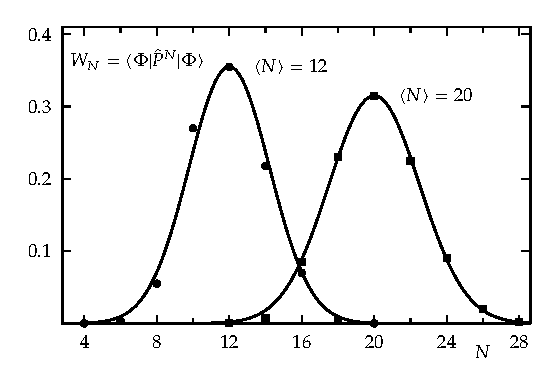
\includegraphics[width=0.6\linewidth]{pictures/11_6}
\par\end{centering}
\centering{}\caption{\label{fig:11_6}稀土区域中实际原子核的BCS基态波函数中具有 $N$ 个粒子、平均数为 $\langle N\rangle={12}$
和 $\langle N\rangle={20}$ 的概率分量。}
\end{figure}

角动量的情况则大不相同。图11.7展示了通过自洽转动模型针对不同 $\left\langle {\widehat{J}}_{x}\right\rangle $
值计算得到的形变良好的原子核 $^{164}\mathrm{{Er}}$ 的内禀波函数中不同角动量的分量 ${W}_{I}$ {[}式（11.150）{]}。现在我们有很强的对称性破缺：
$\left\langle {\Delta{\widehat{\boldsymbol{J}}}^{2}}\right\rangle \simeq{100}$
，这对应于角度上大约 ${10}^{\circ}$ 的展宽，确实是一个相当尖锐的分布。在基态波函数中， $I=0$ 仅由一个相对较小的分量表示。最大值位于
$I\simeq6$ 处。这种意外行为的原因是角动量不是可加量，并且在所考虑的组态空间中，耦合到 $I=6$ 的可能性比耦合到
$I=0$ 的可能性要多得多。由于我们有兴趣以广义直积态的形式考虑尽可能多的关联，我们必须允许存在这样大的赝分量。投影将所有这些分量都设为零。只有在高自旋极限下，分布的最大值才位于
${\widehat{J}}_{x}$ 的平均值处。

\begin{figure}[H]
\begin{centering}
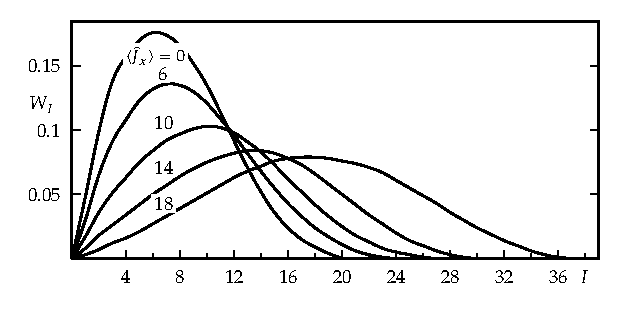
\includegraphics[width=0.62\linewidth]{pictures/11_7}
\par\end{centering}
\centering{}\caption{\label{fig:11_7}对于 $\left\langle {\widehat{J}}_{x}\right\rangle =\sqrt{I\left({I+1}\right)}$
的不同值， $^{164}\mathrm{{Er}}$ 的HFB波函数中具有角动量 $I$ 的概率分量。（源自\cite{IMR79}。）}
\end{figure}




\chapter{时间相关Hartree-Fock方法\label{chap:tdhf}}

\section{引言\label{sec:12.1}}

在描述原子核中涉及大振幅的过程（例如非简谐振动、裂变与聚变过程）的探索中，迄今为止我们仅使用了定态波函数以及 Ritz 变分原理。

另一方面，我们也可以用时间相关的方式来表述这一问题。设在时间 $t=0$ 时以波函数 $|\Psi(0)\rangle$ 出发，它并不是定态多体
Schrödinger 方程的精确解。这样的态代表一个波包（wave packet），其随时间的演化由时间演化算符给出：

\begin{equation}
|\Psi(t)\rangle=\mathrm{e}^{-\mathrm{i}Ht/\hbar}|\Psi(0)\rangle\label{eq:12.1}
\end{equation}

其中 $H$ 为完整的多体 Hamilton 量。时间相关波函数 $|\Psi(t)\rangle$ 中包含的信息在原理上等价于定态
Schrödinger 方程的解，因为对 $|\Psi(t)\rangle$ 进行 Fourier 分析即可给出 $H$ 的能谱及相应的本征态。另一方面，用波包来描述系统更贴近我们的经典直觉。例如在裂变过程中，我们脑海中会浮现出一个在每个时刻都具有确定形变的经典液滴。在微观图景中，这样一个形变态可由形变势阱中的一个
Slater 行列式来表示，它显然不是 $H$ 的本征态，而是\ref{eq:12.1} 意义上的波包。事实上，我们将会看到，在这样一种图景下，在一定的近似下可以导出经典运动方程。

一般拟设\ref{eq:12.1} 对于实际求解而言显然过于复杂。因此，在本章中，我们将分相继的两步作出明确的近似：

(i) 在时间相关 Hartree-Fock（TDHF）理论中，我们以一个 Slater 行列式 $|\Phi(0)\rangle$
出发，并假设它在所有时刻都保持为 Slater 行列式。一般而言，这是一个极强的近似，正如我们将看到的，这在解释计算结果时会带来严重的问题。另一方面，在静态情形中我们已经看到，这一假设的基础在于：由于
Pauli 原理，每个核子并不与其他核子直接发生相互作用，而仅仅与自洽场的势壁相互作用。结合力通过 Brueckner 理论的重整化，以及通过
HFB 理论对配对关联的计入，该近似在整个元素周期表中对基态和单粒子能级都给出了极佳的描述。至少对于单粒子能量远低于 Fermi 能的情况，Pauli
原理在时间相关情形下也应以类似的方式起作用，没有理由认为 HF 近似在动态情形中会失效。存在着广泛的物理现象（例如低激发集体态、核裂变以及中等能量下的重离子碰撞），在这些现象中这种方法都是合理的。因此，我们将在
\ref{sec:12.2} 节中推导作为该理论基础的 TDHF 方程，并讨论它们的性质和所涉及的问题。我们还将介绍若干应用。自然地，计算中使用了密度依赖的相互作用，并且在许多情况下还必须计入配对关联
\cite{Be66,BF76}。由于进行此类计算的方法是显而易见的，我们在此仅针对不含配对关联（$\rho^{2}=\rho$）的纯
Slater 行列式来展示整个理论。

(ii) 在第二步中，我们采用绝热近似（adiabatic approximation），即假定我们系统中的速度很小。将速度展开到二阶便得到了绝热时间相关
Hartree-Fock（ATDHF）理论。它导出的方程在原理上并不比 TDHF 方程更容易求解，但它为理解物理问题提供了极大的洞察力，并允许对所有可用少数集体变量来描述运动的情形导出一个集体
Hamilton 量。这将在 \ref{sec:12.3} 节中予以讨论。

\section{完整的时间相关Hartree-Fock理论\label{sec:12.2}}

\subsection{TDHF方程的推导\label{subsec:12.2.1}}

我们从任意波包 $|\Psi(0)\rangle$ 出发。其精确时间演化由\ref{eq:12.1} 给出，其在时间 $t$
时的单体密度为

\begin{equation}
\rho_{kl}(t)=\langle\Psi(t)|c^{\dagger}_{l}c_{k}|\Psi(t)\rangle\label{eq:12.2}
\end{equation}

为了得到运动方程，我们计算其对时间的一阶导数：

\begin{equation}
\mathrm{i}\hbar\dot{\rho}_{kl}(t)=\langle\Psi(t)|[c^{\dagger}_{l}c_{k},H]|\Psi(t)\rangle\label{eq:12.3}
\end{equation}

对于两体 Hamilton 量 {[}式 $(5.25)${]}，它可以写为

\begin{equation}
\mathrm{i}\hbar\dot{\rho}_{kl}-\sum_{p}(t_{kp}\rho_{pl}-\rho_{kp}t_{pl})=\frac{1}{2}\sum_{prs}(\bar{v}_{kprs}\rho^{(2)}_{rslp}-\bar{v}_{rslp}\rho^{(2)}_{kprs})\label{eq:12.4}
\end{equation}

其中我们引入了两体密度

\begin{equation}
\rho^{(2)}_{klpq}(t)=\langle\Psi(t)|c^{\dagger}_{p}c^{\dagger}_{q}c_{l}c_{k}|\Psi(t)\rangle\label{eq:12.5}
\end{equation}

我们可以用与\ref{eq:12.3} 中处理单体密度相同的方式来推导这一物理量的运动方程。它将两体密度与三体密度联系起来，以此类推（见附录
F）。这一方程组 \cite{BG49} 是精确的，但显然不是闭合的。为了使其闭合，我们必须引入若干近似。\ref{eq:12.4}
的左端描述了系统的自由运动，仅包含动能项；而右端则包含粒子之间的相互作用。这种相互作用可以划分为两部分：一部分是对所有粒子取平均的自洽单体场；另一部分是无法被平均场所计入的两个核子之间的个别碰撞，后者引起了两体关联。

为了实现这种分解，我们通过从 $\rho^{(2)}$ 中扣除无关联对来定义关联函数 $g^{(2)}$：

\begin{equation}
\rho^{(2)}_{klpq}=\rho_{kp}\rho_{lq}-\rho_{kq}\rho_{lp}+g^{(2)}_{klpq}\label{eq:12.6}
\end{equation}

从而代替\ref{eq:12.4}，得到

\begin{equation}
\mathrm{i}\hbar\dot{\rho}_{kl}-[t+\Gamma,\rho]_{kl}=\frac{1}{2}\sum_{prs}(\bar{v}_{kprs}g^{(2)}_{rslp}-\bar{v}_{rslp}g^{(2)}_{kprs})\label{eq:12.7}
\end{equation}

其中密度依赖的 HF 势为

\begin{equation}
\Gamma_{kl}=\sum_{pq}\bar{v}_{kqlp}\rho_{pq}\label{eq:12.8}
\end{equation}

它与静态 HF 理论 {[}式 $(5.34)${]} 中的定义相同。唯一的区别在于它现在包含精确的时间相关密度 $\rho(t)$；因此，自洽场
$\Gamma$ 是时间相关的。

系统中的粒子现在可以经历两种相互作用：与自洽场 $\Gamma$ 的运动势壁发生碰撞，或者与其他粒子发生碰撞。这两种类型都会给系统带来内部激发。因此，我们必须区分由与势壁碰撞所引起的“单体摩擦（one-body
friction）”（见 \cite{MSK77}），以及由\ref{eq:12.7} 右端的两体碰撞所引起的“两体摩擦（two-body
friction）”。

正如我们在引言中所讨论的，在静态情形下，由于 Pauli 原理，两体关联可以忽略。它们可以被归并到 Brueckner 理论中经适当重整化的有效相互作用中。因此我们同样预期，在动态情形下，只要每个粒子的激发能量低于
Fermi 能，$g^{(2)}$ 便可以忽略，两体散射不会起主要作用。在经典极限（$\hbar\to0$）下，这对应于忽略 Boltzmann
方程中的碰撞项，我们将在第 13 章中更详细地讨论这一点。在此情形下，\ref{eq:12.6} 中的两体密度 $\rho^{(2)}$
发生因式分解，可以完全用单体密度 $\rho$ 来表示；于是波函数 $|\Psi(t)\rangle$ 在所有时刻都保持为 Slater
行列式 $|\Phi(t)\rangle$。令 $g^{(2)}=0$，我们最终得到了 TDHF 方程 \cite{Di30}：

\begin{equation}
\mathrm{i}\hbar\dot{\rho}=[h,\rho]\label{eq:12.9}
\end{equation}

其中 $h=t+\Gamma$。这是关于单体密度矩阵 $\rho$ 的非线性矩阵方程，也是关于时间的一阶微分方程。从初始条件 $\rho(0)$
出发，它确定了所有时刻的 $\rho(t)$。\footnote{此方程在核物理中首次由 Ferrell \cite{Fe57} 明确使用。}

在存在外场 $F(t)=\sum_{kl}f_{kl}(t)c^{\dagger}_{k}c_{l}$ 的情况下，对应的 Schrödinger
方程为

\begin{equation}
\mathrm{i}\hbar|\dot{\Psi}(t)\rangle=(H+F(t))|\Psi(t)\rangle\label{eq:12.10}
\end{equation}

即我们必须将\ref{eq:12.3} 中的 Hamilton 量 $H$ 替换为 $H+F(t)$，或者将\ref{eq:12.9}
中的矩阵 $h$ 替换为 $h+f(t)$。这曾被用来推导时间相关外场中的线性响应理论（见 8.5 节）。

在坐标空间中（引入自旋和同位旋变量的方法是显而易见的），对于自旋无关的两体势 $v(\boldsymbol{r},\boldsymbol{r}')$，TDHF
方程 \ref{eq:12.9} 具有如下形式：

\begin{align}
\mathrm{i}\hbar\dot{\rho}(\boldsymbol{r},\boldsymbol{r}',t) & =-\frac{\hbar^{2}}{2m}(\Delta_{\boldsymbol{r}}-\Delta_{\boldsymbol{r}'})\rho(\boldsymbol{r},\boldsymbol{r}',t)+(\Gamma_{H}(\boldsymbol{r})-\Gamma_{H}(\boldsymbol{r}'))\rho(\boldsymbol{r},\boldsymbol{r}',t)\nonumber \\
 & \quad+\int\mathrm{d}^{3}r''\left(\Gamma_{\text{Ex}}(\boldsymbol{r},\boldsymbol{r}'')\rho(\boldsymbol{r}'',\boldsymbol{r}',t)-\Gamma_{\text{Ex}}(\boldsymbol{r}'',\boldsymbol{r}')\rho(\boldsymbol{r},\boldsymbol{r}'',t)\right)\label{eq:12.11}
\end{align}

其中 $\Gamma_{H}$ 和 $\Gamma_{\text{Ex}}$ 的定义见式 $(5.42)$ 及后文。

我们看到，如果我们将 Slater 行列式 $|\Phi(0)\rangle$ 分解为 $A$ 个相互正交的单粒子波函数 $\varphi_{i}(\boldsymbol{r},0)\;(i=1,\dots,A)$，并通过单粒子波函数的
TDHF 方程追踪它们的时间演化：

\begin{equation}
\mathrm{i}\hbar\frac{\partial}{\partial t}\varphi_{i}(\boldsymbol{r},t)=\left(-\frac{\hbar^{2}}{2m}\Delta+\Gamma_{H}(\boldsymbol{r},t)\right)\varphi_{i}(\boldsymbol{r},t)+\int\mathrm{d}^{3}r'\Gamma_{\text{Ex}}(\boldsymbol{r},\boldsymbol{r}',t)\varphi_{i}(\boldsymbol{r}',t)\label{eq:12.12}
\end{equation}

则我们可以得到\ref{eq:12.9} 的一个解 $\rho(t)$。密度 $\rho$ 随后由下式给出：

\begin{equation}
\rho(\boldsymbol{r},\boldsymbol{r}',t)=\sum^{A}_{i=1}\varphi_{i}(\boldsymbol{r},t)\varphi^{*}_{i}(\boldsymbol{r}',t)\label{eq:12.13}
\end{equation}

TDHF 方程的这种形式在实际计算中更易于处理，因为求解依赖于四个坐标 $(\boldsymbol{r},t)$ 的 $A$ 个微分方程，要比求解像\ref{eq:12.11}
那样依赖于七个坐标 $(\boldsymbol{r},\boldsymbol{r}',t)$ 的单个微分方程更为简便。

在讨论 TDHF 方程的性质之前，我们应当指出，它也可以从时间相关变分原理中导出 \cite{KK76}。Lagrange 量定义为

\begin{equation}
\mathcal{L}=\left\langle \Phi(t)\left|\mathrm{i}\hbar\frac{\partial}{\partial t}-H\right|\Phi(t)\right\rangle \label{eq:12.14}
\end{equation}

在 $|\Phi(t)\rangle$ 是单粒子波函数 $\varphi_{1}(\boldsymbol{r},t),\dots,\varphi_{A}(\boldsymbol{r},t)$
的 Slater 行列式\footnote{此变分原理可以被推广。若 $|\Phi\rangle$ 是一个一般的多体波函数，则可以导出精确的 Schrödinger 方程 \cite{KK76}。}的假设下，$\mathcal{L}$
是 $2A$ 个独立场量 $\varphi_{i}(\boldsymbol{r},t)$ 与 $\varphi^{*}_{i}(\boldsymbol{r},t)$
的泛函。将它们视为经典场变量，我们可以在固定的端点 1 和 2 之间定义一个作用量

\begin{equation}
I_{12}=\int^{t_{2}}_{t_{1}}\mathcal{L}[\boldsymbol{\varphi},\boldsymbol{\varphi}^{*}]\,\mathrm{d}t\label{eq:12.15}
\end{equation}

Hamilton 变分原理 \cite{Go59}

\begin{equation}
\delta I_{12}=0\label{eq:12.16}
\end{equation}

对 $\boldsymbol{\varphi}$ 与 $\boldsymbol{\varphi}^{*}$ 进行独立变分，便给出了运动方程
\ref{eq:12.12}。

\subsection{TDHF方程的性质\label{subsec:12.2.2}}

\subsubsection{乘积特性的守恒\label{subsubsec:12.2.2.1}}

在前一节中，我们假设波函数 $|\Phi(t)\rangle$ 在所有时刻都是 Slater 行列式，并在此条件下导出了 TDHF
方程 \ref{eq:12.9}。因此，我们首先必须证明该理论是自洽的，也就是说，如果我们从 Slater 行列式的密度（$\rho^{2}(0)=\rho(0)$）出发，这一性质在所有时刻都是守恒的：

\begin{equation}
\mathrm{i}\hbar\frac{\partial}{\partial t}(\rho^{2}-\rho)=\mathrm{i}\hbar(\dot{\rho}\rho+\rho\dot{\rho}-\dot{\rho})=[h,\rho^{2}-\rho]\label{eq:12.17}
\end{equation}

在第 7 章中，我们详细讨论了当所有 Slater 行列式以适当方式参数化时所得到的能量曲面。因此，TDHF 方程的解 $|\Phi(t)\rangle$
对应于该能量曲面上的一条轨迹。

\subsubsection{正交性的守恒\label{subsubsec:12.2.2.2}}

与刚刚讨论的性质密切相关的事实是：单粒子波函数 $\varphi_{i}(\boldsymbol{r},t)$ 在所有时刻都保持正交：

\begin{equation}
\mathrm{i}\hbar\frac{\partial}{\partial t}\langle\varphi_{i}|\varphi_{k}\rangle=\langle\varphi_{i}|h-h^{\dagger}|\varphi_{k}\rangle=0\label{eq:12.18}
\end{equation}


\subsubsection{对称性算符期望值的守恒\label{subsubsec:12.2.2.3}}

对于任意与时间无关的单粒子算符 $F=\sum f_{lm}c^{\dagger}_{l}c_{m}$，由\ref{eq:12.9}
我们得到在态 $|\Phi(t)\rangle$ 中的期望值满足

\[
\mathrm{i}\hbar\frac{\mathrm{d}}{\mathrm{d}t}\langle F\rangle=\mathrm{i}\hbar\mathrm{Tr}(f\cdot\dot{\rho})=\mathrm{Tr}(f\cdot[h,\rho])
\]

或

\begin{equation}
\mathrm{i}\hbar\frac{\mathrm{d}}{\mathrm{d}t}\langle F\rangle=\langle[F,H]\rangle\label{eq:12.19}
\end{equation}

其中最后一个期望值是利用 Wick 定理（见 C.4 节）计算的。因此，我们发现 Hamilton 量的所有对称性至少在平均意义上都是守恒的。例如：

(i) 粒子数：$(\mathrm{d}/\mathrm{d}t)\langle N\rangle=(\mathrm{d}/\mathrm{d}t)\mathrm{Tr}\rho=0$，式
$(12.20)$；

(ii) 总线动量：$(\mathrm{d}/\mathrm{d}t)\langle\boldsymbol{P}\rangle=0$，式
$(12.21)$；

(iii) 总角动量：$(\mathrm{d}/\mathrm{d}t)\langle\boldsymbol{J}\rangle=0$，式
$(12.22)$。

然而，这并不意味着 $|\Phi\rangle$ 必须是这些对称性算符的本征态。例如，任何定域的密度分布 $\rho(\boldsymbol{r})$
都破坏了平移不变性。我们将在 \ref{subsubsec:12.2.2.5} 节中讨论对称性守恒的问题。

此外，由\ref{eq:12.19}，对于速度无关的相互作用，对于质心 $\boldsymbol{R}=(1/A)\sum\boldsymbol{r}_{i}$
我们得到

\begin{equation}
\frac{\mathrm{d}}{\mathrm{d}t}\langle\boldsymbol{R}\rangle=\frac{1}{Am}\langle\boldsymbol{P}\rangle\label{eq:12.23}
\end{equation}


\subsubsection{能量守恒\label{subsubsec:12.2.2.4}}

能量对时间的全导数可以用密度的变化来表示。由于 $\rho$ 始终保持为 Slater 行列式，在使 $\rho$ 对角化的基底中
$\dot{\rho}$ 仅具有 $ph$ 矩阵元（见 5.3.3 节）：

\begin{equation}
\frac{\mathrm{d}}{\mathrm{d}t}\langle H\rangle=\frac{\mathrm{d}}{\mathrm{d}t}E=\sum_{mi}\left(\frac{\partial E}{\partial\rho_{mi}}\dot{\rho}_{mi}+\frac{\partial E}{\partial\rho_{im}}\dot{\rho}_{im}\right)=\mathrm{Tr}(h\dot{\rho})=\frac{\mathrm{i}}{\hbar}\mathrm{Tr}(h\cdot[\rho,h])=0\label{eq:12.24}
\end{equation}

这意味着能量随时间是守恒的。因此，运动必须在 Slater 行列式的多维能量曲面的等能线上进行。因而，如果我们的初始条件位于某个势谷内，使得能量小于该势谷周围最低的鞍点能量，系统就永远无法离开该势谷。系统将在势谷内的等势线上运行。

在 5.4 节中，我们讨论了 Lipkin 模型中这样一个能量曲面的例子。这里的 HF 能量 $\langle H\rangle$
依赖于两个变量 $\alpha$ 和 $\varphi$。可以将它们变换为一个坐标和正则共轭动量，使得 TDHF 方程成为相应相空间中的经典运动方程
\cite{KLD80}。

\subsubsection{自洽对称性\label{subsubsec:12.2.2.5}}

在 \ref{subsubsec:12.2.2.3} 节中我们看到，精确 Hamilton 量 $H$ 的对称性与相应算符期望值的守恒定律相联系。任何平均场理论的基本特征之一在于波函数和密度可以破坏这些对称性。随着时间的推移，原子核的形变或位置可能会发生剧烈的改变。

然而，正如我们在静态情形中所见到的，可能存在自洽对称性（见 5.5 节）。它们在动态情形中同样会出现：若 $S$ 为一个与 Hamilton
量 $H$ 以及初始密度 $\rho(0)$ 均对易的幺正对称性操作，则 $\rho$ 在所有时刻在该操作下都保持不变。令 $\bar{\rho}=S\rho S^{\dagger}$，我们得到

\begin{equation}
\mathrm{i}\hbar\frac{\partial}{\partial t}(\bar{\rho}-\rho)=[h(\bar{\rho})-h(\rho),\bar{\rho}]+[h(\rho),\bar{\rho}-\rho]\label{eq:12.25}
\end{equation}

即若在时刻 $t$ 对称性是守恒的（$\bar{\rho}=\rho$），则在时刻 $t+\mathrm{d}t$ 它也是守恒的。

这一事实具有数值上的优势，因为可以减小矩阵的维数。然而，在施加对称性时，我们极大地限制了可能的运动，并阻碍了许多关联的发展。即使在对称性破缺对原子核的宏观形状影响不大的情况下，内部的单粒子运动也可能发生剧烈改变，因为自洽对称性限制了每个单独单粒子轨道的自由度。例如在轴对称的情形下，每个核子都必须平行或反平行于对称轴顺排，从而统计涨落受到抑制。换句话说，固定的势壁不会加热系统，为了获得完整的单体耗散（one-body
dissipation），我们必须破缺所有可能的对称性。

若在解 $\rho(t)$ 中破缺了某个连续对称性，正如在静态情形中那样，仅通过施加该对称性操作，我们就能得到无穷多个其他的解。坐标系的平移就是一个例子。

\subsubsection{时间反演不变性\label{subsubsec:12.2.2.6}}

作为 TDHF 方程 \ref{eq:12.9} 动力学解的密度分布 $\rho(t)$ 不是时间反演不变的，其意义在于时间反演算符
\cite[第十五章]{Me61}

\begin{equation}
T=K_{0}\mathrm{e}^{-\mathrm{i}\pi s_{y}}\label{eq:12.26}
\end{equation}

（其中 $K_{0}$ 为复共轭算符）会改变 $\rho$：

\begin{equation}
\rho_{T}(t):=T\rho(t)T^{\dagger}\neq\rho(t)\label{eq:12.27}
\end{equation}

因为 $\rho_{T}=\rho$ 将要求 $\dot{\rho}=0$。另一方面，我们具有微观可逆性（microscopic
reversibility），这意味着 $\rho_{T}(-t)$ 也是 TDHF 方程的一个解。事实上，这一性质常被用来检验求解\ref{eq:12.9}
的计算机程序的精度。然而，这仅仅是微观可逆性，并不意味着系统（在该理论范围内）不能被加热。

\subsection{准静态解\label{subsec:12.2.3}}

\subsubsection{平移\label{subsubsec:12.2.3.1}}

正如我们在上一节中所见，TDHF 方程的动力学解不可能完全是时间偶的。在特殊情况下，我们已经可以通过破坏时间反演对称性的适当变换，从静态
HF 方程的解中求得该方程的动力学解。

此类情形的一个简单例子是变换到以恒定速度 $\boldsymbol{v}$ 运动的参考系的 Galilei 变换。它由算符 $G$
实现（见 \cite[第十五章]{Me61}）：

\begin{equation}
G(\boldsymbol{v},t)=\exp\left(-\frac{\mathrm{i}}{\hbar}\boldsymbol{v}\cdot(mA\boldsymbol{R}-\boldsymbol{P}t)\right)\label{eq:12.28}
\end{equation}

其中 $\boldsymbol{R}=(1/A)\sum\boldsymbol{r}_{i}$ 为质心坐标，$\boldsymbol{P}=\sum\boldsymbol{p}_{i}$
为总动量。与该变换相对应的是单粒子空间中的一个矩阵：$g(\boldsymbol{v},t)=\exp[-(\mathrm{i}/\hbar)\boldsymbol{v}\cdot(m\boldsymbol{r}-\boldsymbol{p}t)]$，它变换密度矩阵：

\begin{equation}
\rho(t)\to\bar{\rho}=g\rho(t)g^{\dagger}\label{eq:12.29}
\end{equation}

$\bar{\rho}$ 满足运动方程

\begin{equation}
0=\mathrm{i}\hbar\dot{\bar{\rho}}=g[h,\rho]g^{\dagger}-g[\boldsymbol{v}\cdot\boldsymbol{p},\rho]g^{\dagger}=[h(\bar{\rho})-\boldsymbol{v}\cdot\boldsymbol{p},\bar{\rho}]\label{eq:12.30}
\end{equation}

利用\ref{eq:12.28} 以及对于速度无关和平移不变相互作用成立的对称性性质 $g\Gamma(\rho)g^{\dagger}=\Gamma(\bar{\rho})$，我们在运动参考系中再次找到了
TDHF 方程：

\begin{equation}
0=\mathrm{i}\hbar\dot{\bar{\rho}}=\left[\frac{1}{2m}(\boldsymbol{p}+m\boldsymbol{v})^{2}+\Gamma(\bar{\rho})-\boldsymbol{v}\cdot(\boldsymbol{p}+m\boldsymbol{v}),\bar{\rho}\right]=[h(\bar{\rho}),\bar{\rho}]\label{eq:12.31}
\end{equation}

由此我们看到，运动参考系中的静态解 $[h(\bar{\rho}),\bar{\rho}]=0$ 变换成了实验室参考系中 TDHF
方程的非平凡动力学解。它具有如下形式：

\begin{equation}
\rho(t)=\mathrm{e}^{(\mathrm{i}/\hbar)m\boldsymbol{v}\cdot\boldsymbol{r}}\left(\mathrm{e}^{-(\mathrm{i}/\hbar)\boldsymbol{v}\cdot\boldsymbol{p}t}\bar{\rho}\mathrm{e}^{(\mathrm{i}/\hbar)\boldsymbol{v}\cdot\boldsymbol{p}t}\right)\mathrm{e}^{-(\mathrm{i}/\hbar)m\boldsymbol{v}\cdot\boldsymbol{r}}\label{eq:12.32}
\end{equation}

这表明定态解 $\bar{\rho}$ 首先经历坐标的时间偶平移量 $-\boldsymbol{v}t$，然后通过动量的时间奇变换获得一个速度。在坐标空间中，我们得到

\begin{equation}
\rho(\boldsymbol{r},\boldsymbol{r}',t)=\mathrm{e}^{(\mathrm{i}/\hbar)m\boldsymbol{v}\cdot(\boldsymbol{r}-\boldsymbol{r}')}\cdot\mathrm{e}^{-\boldsymbol{v}t\cdot(\boldsymbol{\nabla}_{\boldsymbol{r}}+\boldsymbol{\nabla}_{\boldsymbol{r}'})}\bar{\rho}(\boldsymbol{r},\boldsymbol{r}')\label{eq:12.33}
\end{equation}

在时刻 $t=0$ 时，对角密度 $\rho(\boldsymbol{r},\boldsymbol{r},0)$ 与定态值 $\bar{\rho}$
完全相同。集体速度仅通过非对角部分中依赖于 $\boldsymbol{r}$ 的相位因子表现出来。

在 TDHF 理论应用于重离子反应的实际计算中，人们通常采用两个形如\ref{eq:12.33} 且速度分别为 $\boldsymbol{v}_{1}$
和 $\boldsymbol{v}_{2}$、相隔距离足够远而不发生重叠的密度之和作为初始条件。在很好的近似下，它们代表在反应发生之前处于基态的两个运动离子。

\subsubsection{转动\label{subsubsec:12.2.3.2}}

在转动的情形下，我们也希望变换到一个转动参考系，在该参考系中运动可以用静态解来描述。然而与平移不同，转动集体运动是非平凡的。在此种情形下不存在“质心角”，也不存在
Galilei 不变性（见 11.3.3 节）。尽管如此，我们可以执行变换 \ref{eq:12.28} 的第一部分，即将坐标变换到以角速度
$\boldsymbol{\omega}$ 转动的参考系：

\begin{equation}
\tilde{\rho}=\mathrm{e}^{\mathrm{i}\boldsymbol{\omega}\cdot\boldsymbol{j}t}\rho(t)\mathrm{e}^{-\mathrm{i}\boldsymbol{\omega}\cdot\boldsymbol{j}t}\label{eq:12.34}
\end{equation}

类比于\ref{eq:12.30}，我们得到

\begin{equation}
\mathrm{i}\hbar\dot{\tilde{\rho}}=\mathrm{e}^{\mathrm{i}\boldsymbol{\omega}\cdot\boldsymbol{j}t}[t+\Gamma(\rho)-\boldsymbol{\omega}\cdot\boldsymbol{j},\rho]\mathrm{e}^{-\mathrm{i}\boldsymbol{\omega}\cdot\boldsymbol{j}t}=[h(\tilde{\rho})-\boldsymbol{\omega}\cdot\boldsymbol{j},\tilde{\rho}]\label{eq:12.35}
\end{equation}

现在我们得到了自洽 Cranking 模型的定态 HF 问题（见 7.7 节和 11.4.6.3 节）：

\begin{equation}
[h(\tilde{\rho})-\boldsymbol{\omega}\cdot\boldsymbol{j},\tilde{\rho}]=0\label{eq:12.36}
\end{equation}

它给出了一个不具时间依赖性但包含时间奇分量的密度 $\tilde{\rho}$。在此意义上它并不是静态密度。同样，

\begin{equation}
\rho(t)=\mathrm{e}^{-\mathrm{i}\boldsymbol{\omega}\cdot\boldsymbol{j}t}\tilde{\rho}\mathrm{e}^{\mathrm{i}\boldsymbol{\omega}\cdot\boldsymbol{j}t}\label{eq:12.37}
\end{equation}

是 TDHF 方程 \ref{eq:12.9} 的一个非平凡解。

\ref{eq:12.36} 也可以从投影 TDHF 理论以如下方式更根本地导出 \cite{EMR80b}。类比于\ref{eq:12.14}，我们从
Lagrange 量出发：

\[
\mathcal{L}=\left\langle \Phi(t)\left|\hat{P}^{I}\left(\mathrm{i}\hbar\frac{\partial}{\partial t}-H\right)\hat{P}^{I}\right|\Phi(t)\right\rangle 
\]

其中 $\hat{P}^{I}$ 是好角动量投影算符（见 11.4.6 节）。作用量 \ref{eq:12.15} 对时间相关的
Slater 行列式 $|\Phi(t)\rangle$ 的变分便给出了投影 TDHF 方程。在大形变极限下，我们可以使用一阶 Kamlah
展开 {[}式 $(11.80)${]} 并得到\ref{eq:12.35}。其最简单的解由定态问题 \ref{eq:12.36}
给出。

如果相信 Cranking 模型，人们便可通过这种方式看出：投影在时间相关 HF 情形下是一个非常重要的特征。这在其他问题中也变得显而易见，例如在反应截面的计算中，我们必须向各个反应道进行投影（见
\ref{subsec:12.2.4} 节）。

\subsection{TDHF方法的一般讨论\label{subsec:12.2.4}}

乍看起来，TDHF 方法似乎具有极具吸引力的优势。它为原子核中各类集体运动提供了统一的描述：从基态的静态解出发，历经转动与振动激发，直至大振幅集体运动，诸如裂变、聚变、复合核形成以及深部非弹性反应。系统能够在多维能量曲面上自行决定其演化路径，该能量曲面包含了所有可由乘积态表示的构型。特别地，我们无需先验地选取某些集体坐标，也无需迫使系统在非物理的外场中运动。我们无需预先了解系统内部的流动模式，也无需知道惯性参数及其对坐标的依赖关系。

另一方面，这一概念并不仅仅描述集体现象：在所有时刻波函数都保持为 Slater 行列式。它兼顾了单粒子结构的所有方面，并包含了集体运动与单粒子运动之间的完全相互作用。

最后，TDHF 方程的解还包含了摩擦与阻尼效应，只要这些效应是由粒子与时间相关平均场的势壁相互作用所产生的——即所谓的单体摩擦（one-body
friction，见 \cite{BBN78} 及其所列参考文献）。

为了看清在巨共振情形下这种阻尼的来源，我们利用 Thouless 定理 {[}式 $(\text{E}.26)${]}，在 HF
基态 $|\Phi_{0}\rangle$ 的基底中展开 $|\Phi(t)\rangle$：

\begin{align}
|\Phi(t)\rangle & \propto\exp\left(\sum_{mi}z_{mi}(t)a^{\dagger}_{m}a_{i}\right)|\Phi_{0}\rangle\nonumber \\
 & =|\Phi_{0}\rangle+\sum_{mi}z_{mi}(t)a^{\dagger}_{m}a_{i}|\Phi_{0}\rangle+\sum_{mim^{\prime}i^{\prime}}z_{mi}(t)z_{m^{\prime}i^{\prime}}(t)a^{\dagger}_{m}a^{\dagger}_{m^{\prime}}a_{i^{\prime}}a_{i}|\Phi_{0}\rangle+\dots\label{eq:12.38}
\end{align}

我们看到，除了 ph 掺杂（这在第 8 章的 TDA 或 RPA 中已经处理过）之外，TDHF 波函数还包含 2p2h、3p3h 分量等等。为了得到这些掺杂成分随能量变化的强度，我们必须对
$|\Phi(t)\rangle$ 进行 Fourier 变换。

迄今为止，尚不清楚巨共振的扩散宽度\footnote{然而我们应当注意，TDHF 理论包含了正如在 8.5.4 节中所讨论的逃逸宽度（escape width），这意味着粒子实际上正在离开原子核。}中有多少来自此类
2p2h 掺杂（单体摩擦），以及略去\ref{eq:12.7} 中的碰撞项 $I(\rho)$ 或\ref{eq:12.7}
中的 $g^{(2)}$ 项（二体摩擦）在多大程度上是正确的。\ref{eq:12.7} 中 $g^{(2)}$ 项可以忽略的近似，反过来又基于这样一种观点
\cite{KK68}：由于 Pauli 不相容原理，核子的平均自由程与核线度具有相同的数量级。这一假设的有效性在每粒子能量达到
Fermi 能数量级时必然失效，但仍有广泛的现象我们应当能够用 TDHF 方法来描述。

特别地，该理论并不必然受限于绝热假设——即波函数在每一时刻都非常接近相应自洽势阱 $h(t)$ 的基态。对于动态解而言，TDHF
单粒子函数 $\phi_{i}(t)$ {[}\ref{eq:12.12}{]} 与该势阱中的本征函数是不同的：

\begin{equation}
h(t)|\psi_{k}(t)\rangle=\epsilon_{k}(t)|\psi_{k}(t)\rangle\label{eq:12.39}
\end{equation}

这意味着我们并不能通过填满势阱 $h(t)$ 中的最低 $A$ 个能级来获得 TDHF Slater 行列式 $|\Phi(t)\rangle$。密度
$\rho(t)$ 与 $h(t)$ 并不对易，也就是说，$\rho(t)$ 在本征函数 $|\psi_{k}(t)\rangle$
构成的基底中不是对角的，占有几率 $\rho_{k}$（即 $\rho$ 在该基底下的对角元）：

\begin{equation}
\rho_{k}(t)=\langle\psi_{k}(t)|\rho(t)|\psi_{k}(t)\rangle\label{eq:12.40}
\end{equation}

弥散分布在许多能级上，即我们在该基底中得到了一个弥散开的 Fermi 面。另一方面，占有几率的分布也不应过分偏离 Fermi 阶跃函数，即它不应变得完全碎裂，否则不相容原理将不再能够压低二体碰撞。然而，目前对这一问题尚无详细的研究。

尽管 TDHF 方法具有所有这些巨大的优点，但我们必须清醒地认识到该方法存在着某些重要的局限性：

(i) 该理论提供了一种完全微观的描述，它跟踪每个单粒子波函数随时间的变化，因而需要耗费极其巨大的数值计算量。特别地，我们应当牢记：只有当尽可能多的对称性被破缺时，它的全部优势与威力才能展现出来。这种类型的现实计算不仅接近现代计算机算力的极限，而且往往极难从中提取出系统的基本物理特征并借助简明模型加以理解。

(ii) 在某种意义上，该理论表现出经典的确定性行为：我们从一个初始密度 $\rho(t)$ 出发，并在多维能量曲面上跟踪它及其速度
$\dot{\rho}(t)$ 随时间的演化，正如一条经典轨道。仅凭这一事实并不能断言该理论是经典的；精确的量子力学统计算符 $\rho$
服从 von Neumann 方程，其结构与\ref{eq:12.9} 极为相似。与完全量子力学理论的根本差异在于：我们在所有时刻都将波函数限制为
Slater 行列式，从而导出了一个非线性方程。因此我们放弃了态叠加原理，即两个 Slater 行列式的线性组合（一般而言）不再是一个乘积波函数。作为理论非线性的必然结果，我们得到了具有孤子（soliton）特性的解（见
12.2.5 节），即在传播过程中保持形状不变的密度分布 {[}例如见\ref{eq:12.32}{]}，而精确的量子力学密度 $\rho(\boldsymbol{r})=\langle\Psi(t)|\hat{\rho}(\boldsymbol{r})|\Psi(t)\rangle$
必然会表现出通常的量子力学波包弥散。以恒定速度运动的静态密度这一例子 {[}\ref{eq:12.32}{]} 不出现弥散的事实，也可以表述为我们在
TDHF 理论中破坏了平移不变性，即我们处于原子核的内禀参考系中，并将核质心坐标与其动量视为两个可同时测量的（经典）量。这当然与将
Slater 行列式视为精确波函数的近似紧密相关。

(iii) 另一个量子力学效应是穿透势垒的隧道效应。如果我们在能量曲面上有两个分离的局域极小值，并且我们从一个谷中以小于两极小值间最低鞍点的能量出发，由于能量守恒
{[}\ref{eq:12.24}{]}，系统将永远无法到达另一个谷。存在两个不同的谷正是非线性的结果。线性理论永远只有一个极小值，即基态（见
5.2 节）。隧道效应的不可能性在将一般 Slater 行列式集合限制为具有少数集体自由度的乘积波函数 $|\Phi(q)\rangle$
的情形下（见 12.3.3 节，如裂变过程的描述）变得尤为明显。在此类情形中，我们必须要么重新量子化，要么引入乘积态的线性叠加。这把我们带回了生成坐标法（第
10 章）。

在 Slater 行列式空间中的势垒（最终过渡为集体坐标下的势垒），不应与坐标空间中外场 $V(\boldsymbol{r})$
的势垒相混淆。例如，让我们研究一个以确定速度朝向此类外势垒运动的静态解。该系统的波函数 $|\Phi\rangle$ 由单粒子波函数
$\phi_{i}(\boldsymbol{r})$ 的乘积构成。其中每一个波函数都有一个穿透势垒的尾巴。因此一般而言，$|\Phi\rangle$
在该势垒处分裂为两部分：透射部分与反射部分。这两部分各自单独来看都不再是 Slater 行列式，且单粒子波函数 $\phi_{i}$
同时属于这两部分。取决于入射能量，透射与反射部分具有非常不同的大小。\ref{fig:12.1}(a) 给出了在一维计算中的结果，其中一块核物质厚板以每核子能量等于势垒高度的动能向高斯形势垒运动。我们看到整块厚板全部被透射过去。如果没有粒子间通过平均场的相互作用，我们本预期每个单粒子波函数的透射几率仅为
0.5。然而，自洽场与外势垒共同作用，为粒子提供了一个急剧减小的有效势垒。\ref{fig:12.1}(b) 给出了在更高势垒下的同一过程。此时初始厚板分裂为两部分。我们再次观察到，集体穿透几率远高于单个粒子的穿透几率。

\begin{figure}[H]
\begin{centering}
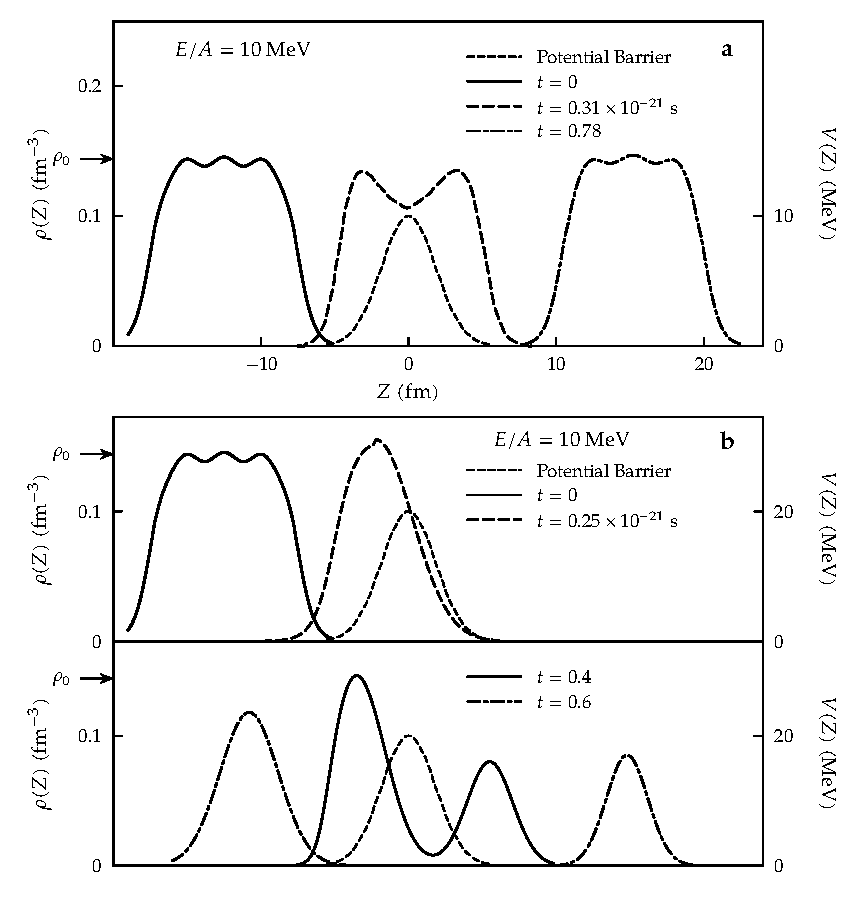
\includegraphics[width=0.85\textwidth]{pictures/12_1}
\par\end{centering}
\caption{\label{fig:12.1}核物质厚板与高度为 10 MeV (a) 和 20 MeV (b) 的高斯势垒的相互作用。（引自
\cite{BKN76}）}
\end{figure}

(iv) 在对波函数 $|\Phi(t)\rangle$ 所包含结果的物理解释中存在着根本性问题。这已经在厚板朝向外势垒运动的例子中显现出来：整块厚板是以某种几率完全穿透，还是在每次碰撞中都碎裂为两个独立的部分，其质量对应于势垒左右两侧积分密度
$|\phi_{i}|^{2}$？在后一种情形下，我们将在每个部分中得到非整数的粒子数，因为正如我们所指出的，散射后的碎片自身不再是
Slater 行列式；从而单粒子波函数同时归属于所有碎片。我们还可以设想这两种可能性的复杂混合。在物理上，我们感兴趣的是 $A_{1}$
个粒子透射而 $A_{2}=A-A_{1}$ 个粒子被反射的几率，即在 $t\to\infty$ 的极限下势垒左侧有 $A_{2}$
个粒子而右侧有 $A_{1}$ 个粒子的几率：

\begin{equation}
P_{A_{1}A_{2}}=\frac{(A_{1}+A_{2})!}{A_{1}!A_{2}!}\int^{\infty}_{0}\mathrm{d}x_{1}\dots\mathrm{d}x_{A_{1}}\int^{0}_{-\infty}\mathrm{d}x_{A_{1}+1}\dots\mathrm{d}x_{A}|\Phi(x_{1}\dots x_{A},t\to\infty)|^{2}\label{eq:12.41}
\end{equation}

这是计算质量分布的一个实用处方，它也已被应用于重离子碰撞的计算中 \cite{Ke76}。

然而在一般情形下，我们希望知道此类反应中不同反应道的 $S$ 矩阵元。能否从 TDHF 计算中获取此类信息是一个悬而未决的问题。原则上，我们可以将
TDHF 方程的波包 $|\Phi(t)\rangle$ 视为精确波包 $|\Psi(t)\rangle$ 的有效近似，从而完全像拥有
$|\Psi(t)\rangle$ 时那样从 $|\Phi(t)\rangle$ 获取 $S$ 矩阵元；例如，我们可以将 $|\Phi\rangle$
投影到模型散射态上。然而，这将意味着计算两个不同多体波函数的重叠，这可能导致极为严重的错误结果，正如下面的考量所示：假设我们计算两个仅有极微小差别的乘积波函数的重叠，其中一个行列式中的所有单粒子波函数与另一个行列式中的波函数处处相差一个微小量
$\epsilon$：

\begin{equation}
(1-\epsilon)^{A}\simeq\mathrm{e}^{-\epsilon A}\label{eq:12.42}
\end{equation}

即对于大粒子数，重叠指数式地微小。如果我们希望计算（例如）静态 HF 波函数与精确波函数的重叠，情况也是如此，其中我们可以假设由于关联效应，每个单粒子轨道以几率
$\epsilon$ 被耗尽（depleted）\cite{Ne77}。尽管 HF 波函数与精确波函数的重叠极小，我们在结合能等方面却依然能获得极佳的结果。这是因为在那里我们只需要计算单体和二体算符的期望值，它至多只涉及两个单粒子波函数。同样的考量在时间相关情形下也成立：从
$|\Phi(t)\rangle$ 计算 $S$ 矩阵元（见上文）意味着在重离子反应情形下我们要计算 $A$ 体算符的期望值（全部
$A$ 个核子的构型均发生了改变），因此这很可能给出相当不可靠的结果。所以在时间相关情形下，我们也必须将自己限制在计算少体算符（诸如粒子数分布、平均能量损失和动量转移）的均值及其涨落上。

与上述问题密切相关的是：从一个 Slater 行列式作为初始条件出发，精确波函数 $|\Psi(t)\rangle$ 在时间演化过程中是否能够保持接近于一个
Slater 行列式。为此，Lichtner 和 Griffin \cite{LG76a} 研究了如下函数的时间相关性：

\begin{equation}
D(t)=\frac{1}{A}\mathrm{Tr}(\rho(t)-\rho^{2}(t))\label{eq:12.43}
\end{equation}

在 $t=0$ 时以 Slater 行列式 $|\Phi_{0}\rangle$ 出发，在短时间内我们发现：

\begin{equation}
D(t)=\left(\frac{t}{\tau}\right)^{2}+\dots\label{eq:12.44}
\end{equation}

其寿命有一个极限：

\begin{equation}
\frac{1}{\tau}\geqslant\frac{2}{\hbar}\sqrt{\frac{1}{A}\left(\langle\Phi_{0}|H^{2}|\Phi_{0}\rangle-\langle\Phi_{0}|H|\Phi_{0}\rangle^{2}\right)}\label{eq:12.45}
\end{equation}

它与函数 $|\Phi_{0}\rangle$ 中每核子的能量弥散成正比。对于真实核，我们发现 $\tau$ 的值在 $10^{-22}$
到 $10^{-21}$ 秒之间。这意味着仅仅在极短的时间之后，波函数 $|\Psi(t)\rangle$ 就已经看起来与 Slater
行列式大相径庭。这再次表明：一旦 $|\Psi(t)\rangle$ 与 $|\Phi(t)\rangle$ 出现微小偏差，重叠
$\langle\Psi(t)|\Phi(t)\rangle$ 就会变得极小；但这并不意味着 $|\Phi(t)\rangle$
不能用于计算少体算符的期望值。

(v) 也许 TDHF 理论中最严重的问题是末态赝相互作用（spurious final state interaction）。在精确计算中，我们将拥有许多不同的出射道，它们在
$t\to\infty$ 时彼此不发生相互作用。在我们厚板朝向势垒运动的例子中，我们可以考虑（例如）穿透一个、两个或三个粒子，而其余粒子被反射。通常，透射系统将具有不同的速度。然而在
TDHF 理论内部，所有反应道都被束缚在势垒右侧的一个共同平均势阱中。为了留在该势阱内，所有反应道都必须持久地交换动量。因此在长时间演化后，我们在不同反应道之间也得到了非物理的赝相互作用。即使我们不计算
$S$ 矩阵元，我们也无法排除这种末态相互作用会对少体算符的平均值产生虚假贡献。类比于静态 HF 问题中的对称性破坏，我们因此应当对各个反应道进行某种投影后变分（见第
11 章）。TDHF 波函数 $|\Phi(t)\rangle$ 必须被理解为一个“内禀”波函数。

事实上，人们可以从精确量子力学传播子的 Feynman 路径积分表象 \cite{FH65} 的鞍点近似中导出 TDHF 方程 \cite{KI77,ER78,NLP79,Re79}，在其中上述问题似乎得到了更为妥善的处理。

\subsection{一个精确可解模型\label{subsec:12.2.5}}

为了研究上述讨论的某些问题，Yoon 和 Negele \cite{YN77} 研究了一个由 $N$ 个玻色子在一维中通过 $\delta$
力相互作用的精确可解模型。\footnote{类似但更为复杂的模型已针对费米子系统被提出 \cite{NW76a,NW78}。}其
Hamilton 量由下式给出：

\begin{equation}
H=-\frac{1}{2}\sum^{N}_{i=1}\frac{\partial^{2}}{\partial x^{2}_{i}}-v\sum^{N}_{i<j=1}\delta(x_{i}-x_{j})\label{eq:12.46}
\end{equation}

该模型对束缚态 \cite{Be31,Mc65} 以及散射态 \cite{Ya67} 都已被精确求解。为了得到所有玻色子在自洽场中占据波函数为
$\phi(x,t)$ 的最低能级的乘积态的时间相关 Hartree 方程，我们使用变分原理\ref{eq:12.16}：

\begin{equation}
\langle\Phi|\mathrm{i}\frac{\partial}{\partial t}-H|\Phi\rangle=N\int\mathrm{d}x\left(\phi^{*}\mathrm{i}\frac{\partial}{\partial t}\phi+\frac{1}{2}\phi^{*}\frac{\partial^{2}}{\partial x^{2}}\phi+\frac{v}{2}(N-1)\phi^{*}\phi^{*}\phi\phi\right)\label{eq:12.47}
\end{equation}

并求得：

\begin{equation}
\mathrm{i}\frac{\partial}{\partial t}\phi+\frac{1}{2}\frac{\partial^{2}}{\partial x^{2}}\phi+v(N-1)\phi^{*}\phi\phi=0\label{eq:12.48}
\end{equation}

其静态解为：

\begin{equation}
\phi_{s}(x)=\frac{\sqrt{(N-1)v}}{2\cosh((N-1)vx/2)}\label{eq:12.49}
\end{equation}

能量为：

\begin{equation}
E_{H}=-\frac{N(N-1)^{2}v^{2}}{24}\label{eq:12.50}
\end{equation}

密度为：

\begin{equation}
\rho_{s}(x)=\frac{N(N-1)v}{4\cosh^{2}((N-1)vx/2)}\label{eq:12.51}
\end{equation}

在 $2N$ 个粒子的动态情形下，\ref{eq:12.48} 具有双孤子解 \cite{ZS72,Do76}（关于孤子的定义与性质，参见综述文章
\cite{SCM73,Ra75}）：

\begin{equation}
\phi(x,t)=\frac{\sqrt{(2N-1)v}}{2}\mathrm{e}^{-(\mathrm{i}/2)(K^{2}-a^{2})t}\frac{\left(\mathrm{e}^{\mathrm{i}Kx}\left\{ \mathrm{e}^{-a(x-Kt)}+\left[K^{2}/(K-\mathrm{i}a)^{2}\right]\mathrm{e}^{-a(3x+Kt)}\right\} \right)+(K\leftrightarrow-K)}{1+2\mathrm{e}^{-2ax}\cosh(2aKt)-2a^{2}\mathrm{e}^{-2ax}\mathrm{Re}\left(\mathrm{e}^{2\mathrm{i}Kx}/(K+\mathrm{i}a)^{2}\right)+\left(K^{4}/(K^{2}+a^{2})^{2}\right)\mathrm{e}^{-4ax}}\label{eq:12.52}
\end{equation}

其中 $4a=(2N-1)v$，且 $K$ 为任意实数。它描述了两个相对动量为 $2K$ 的孤波彼此穿过对方的过程。该波函数是在质心参考系中给出的。为了求出其中一个波包参考系中的密度，我们令
$y=x-Kt$ 并得到：

\begin{equation}
\rho(y,t)=2N\cdot|\phi(y,t)|^{2}\underset{t\to\infty}{=}\frac{N(N-\frac{1}{2})v}{4\cosh^{2}((N-\frac{1}{2})vy/2)}\label{eq:12.53}
\end{equation}

对于大 $N$ 值，它与静态密度\ref{eq:12.51} 相一致。我们还可以证明，两波包相互穿透所产生的时间延迟在大 $N$
极限下与精确的时间延迟相符 \cite{Do76}。另一方面，行列式的寿命\ref{eq:12.45} 对于大 $N$ 趋于零。因此，该模型为我们提供了一个范例：源自平均场理论的结果在大系统极限下可能是精确的，即使其波函数与精确波函数的重叠为零。

\subsection{TDHF理论的应用\label{subsec:12.2.6}}

TDHF 理论最早的应用是在小振幅极限下描述围绕静态解 $\rho_{0}$ 的振动。在第 8 章中我们已经看到，将\ref{eq:12.9}
对 $\delta\rho=\rho-\rho_{0}$ 线性化便导出了随机相位近似（RPA）。

在小速度 $\dot{\rho}$ 但大振幅的极限下，我们得到绝热 TDHF 理论（ATDHF）。这将在 12.3 节中连同其应用一起讨论。因此，我们在本节中将局限于
TDHF 方程 \ref{eq:12.9} 的精确数值解。

TDHF 理论已被应用于精确可解模型中。我们在上一小节给出了这样一个范例。另一个例子是 Lipkin 模型 \cite{Kr77,KLD80}。图
5.3 展示了该模型的能量曲面。TDHF 方程的解即为等能线 \cite{KLD80}。

在所有更为现实的计算中 \cite{BKN76,KDM77,CMM78,BGK78,FKW78}，都采用了 Skyrme 型相互作用力。有限力程修正（$t_{1}p^{2}$）被略去，或者在某些情形下被具有有限力程的
Yukawa 力所取代，该力带有特殊的交换部分，使其仅对自洽势的直接项产生贡献。Coulomb 力中的交换项也被略去。这样，\ref{eq:12.12}
仅为一个微分方程，而不是在一般情形下那样的积分微分方程。

为了进一步简化，我们将讨论限制在一维核物质厚板的情形，此时所有单粒子波函数仅依赖于坐标 $z$：

\begin{equation}
\mathrm{i}\hbar\dot{\phi}_{i}(z,t)=\left(-\frac{\hbar^{2}}{2m}\frac{\partial^{2}}{\partial z^{2}}+\Gamma(z,t)\right)\phi_{i}(z,t)=h(z,t)\phi_{i}(z,t)\label{eq:12.54}
\end{equation}

对坐标 $z$ 进行空间离散化得到一个矩阵方程：

\begin{equation}
\mathrm{i}\hbar\dot{\boldsymbol{\phi}}(t)=h(t)\boldsymbol{\phi}(t)\label{eq:12.55}
\end{equation}

最后，对时间 $t$ 也进行离散化。显而易见的推进方式是：

\begin{equation}
\mathrm{i}\hbar\frac{1}{\Delta t}(\boldsymbol{\phi}^{(n+1)}-\boldsymbol{\phi}^{(n)})=h^{(n)}\boldsymbol{\phi}^{(n)}\label{eq:12.56}
\end{equation}

或：

\begin{equation}
\boldsymbol{\phi}^{(n+1)}=\left(1-\frac{\mathrm{i}}{\hbar}\Delta t\cdot h^{(n)}\right)\boldsymbol{\phi}^{(n)}\label{eq:12.57}
\end{equation}

由于 $(1-(\mathrm{i}/\hbar)\Delta t\cdot h^{(n)})$ 不是幺正的，这会导致数值不稳定性。避免这一问题的方法是用下式代替\ref{eq:12.56}：

\begin{equation}
\mathrm{i}\hbar\frac{1}{\Delta t}(\boldsymbol{\phi}^{(n+1)}-\boldsymbol{\phi}^{(n)})=\frac{1}{2}h^{(n)}(\boldsymbol{\phi}^{(n+1)}+\boldsymbol{\phi}^{(n)})\label{eq:12.58}
\end{equation}

或：

\begin{equation}
\boldsymbol{\phi}^{(n+1)}=\frac{1-\frac{\mathrm{i}}{2\hbar}\Delta t\cdot h^{(n)}}{1+\frac{\mathrm{i}}{2\hbar}\Delta t\cdot h^{(n)}}\boldsymbol{\phi}^{(n)}\label{eq:12.59}
\end{equation}

采用时间演化算符的幺正近似（即所谓的 Crank-Nicholson 算符 \cite{CN47}）。然而该方程涉及矩阵求逆，最近将时间演化算符的
Taylor 级数截断至前几项的方法已被证明具有令人满意的精度 \cite{FKW78}。

相互作用力的力常数通过在静态情形下重现核物质性质来确定。为了研究单个厚板的振荡，初始条件选取为：

\begin{equation}
\phi_{i}(\boldsymbol{r},t=0)=\mathrm{e}^{\mathrm{i}S(\boldsymbol{r})}\phi^{0}_{i}(\boldsymbol{r})\label{eq:12.60}
\end{equation}

其中 $\phi^{0}_{i}$ 为静态单粒子波函数。函数 $S(\boldsymbol{r})$ 决定了 $t=0$ 时的速度分布，该速度分布由流密度
$\boldsymbol{j}(\boldsymbol{r},t)$ 的分布所定义：

\begin{equation}
\boldsymbol{v}(\boldsymbol{r},t)=\frac{\boldsymbol{j}(\boldsymbol{r},t)}{\rho(\boldsymbol{r},t)}=\frac{1}{\rho(\boldsymbol{r},t)}\sum^{A}_{i=1}\frac{\hbar}{2m\mathrm{i}}(\phi^{*}_{i}\boldsymbol{\nabla}\phi_{i}-\phi_{i}\boldsymbol{\nabla}\phi^{*}_{i})\label{eq:12.61}
\end{equation}

或：

\begin{equation}
\boldsymbol{v}(\boldsymbol{r},t=0)=\frac{\hbar}{m}\boldsymbol{\nabla}S(\boldsymbol{r})\label{eq:12.62}
\end{equation}

对于 $S(\boldsymbol{r})=\alpha z^{2}$，我们得到 $v(z)=(2\hbar/m)\alpha z$。在此初始条件下，厚板开始振荡。\ref{fig:12.2}展示了对应于呼吸模的此类振动随不同
$\alpha$ 值的变化情况。即使对于很小的 $\alpha$，这些振荡也是非简谐的，并且似乎并不对应于单一频率。对于较大的
$\alpha$ 值，振荡表现出急剧的涨落。最后，当激发过强时，厚板碎裂为碎片（图中未绘出）。

\begin{figure}[H]
\begin{centering}
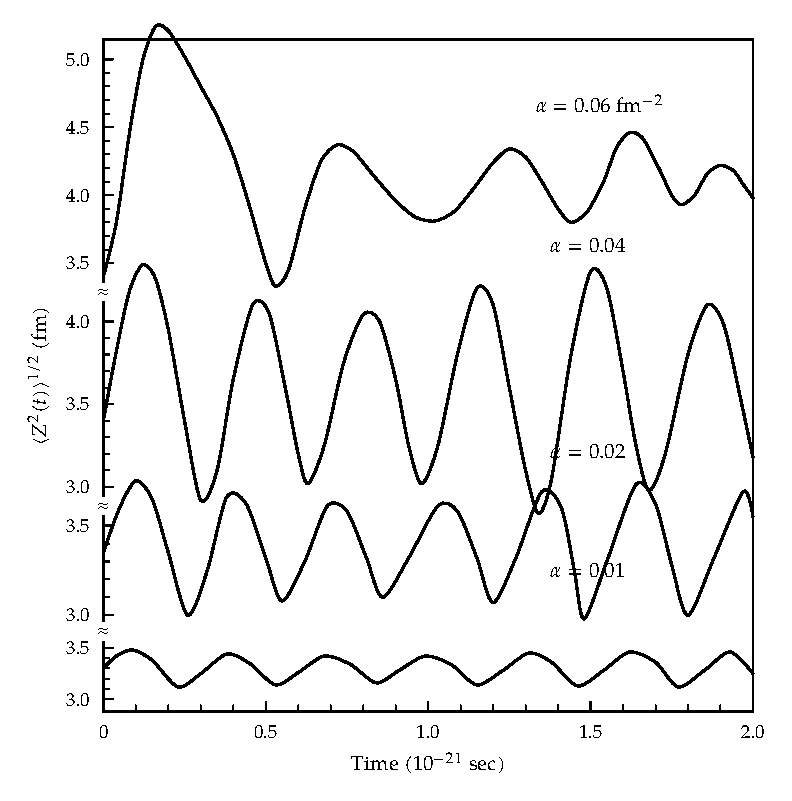
\includegraphics[width=0.8\textwidth]{pictures/12_2}
\par\end{centering}
\caption{\label{fig:12.2}不同初始速度参数 $\alpha$ 下，TDHF 近似中振荡核物质厚板的均方根长度随时间的变化。（引自
\cite{BKN76}）}
\end{figure}

从两个向相反方向运动的自洽厚板出发，我们可以研究碰撞过程。我们发现了丰富多样的现象。取决于入射能量，人们观察到了非弹性散射、复合核形成、共振行为、强阻尼碰撞、转移过程以及碎裂。\ref{fig:12.3}展示了在居中能量下不同时刻的
$\rho(z,t)$。在经历初态聚变后中心密度增加。复合系统开始振荡并在一个周期后发生裂变。

\begin{figure}[H]
\begin{centering}
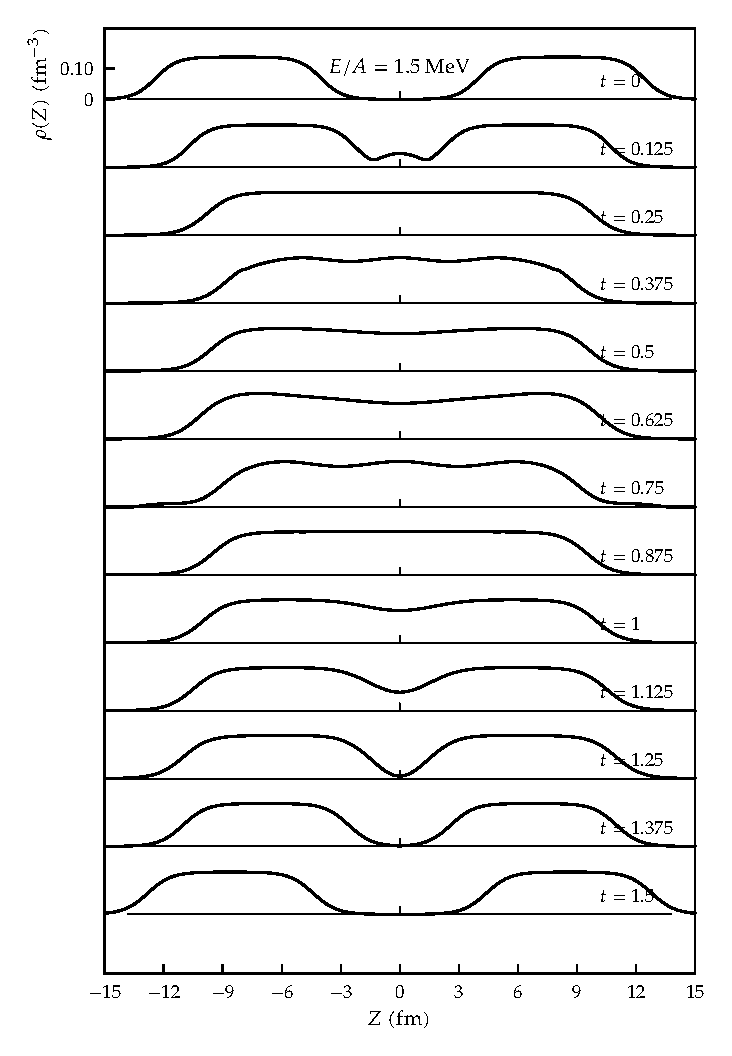
\includegraphics[width=0.75\textwidth]{pictures/12_3}
\par\end{centering}
\caption{\label{fig:12.3}居中能量下两个相同核物质厚板碰撞散射在不同时刻的密度剖面 $\rho(z,t)$。（引自 \cite{BKN76}）}
\end{figure}

在其他能量下则发生聚变。正如我们在\ref{fig:12.4}中所见，我们在低能下总是得到聚变，而在高能下复合系统总是发生破裂；在此二者之间存在一个共振区。具体而言，这极大程度上取决于断裂点处颈部区域内的单粒子运动。如果单粒子效应在关键时刻在该区域产生了耗尽，就会发生断裂；否则系统将反向振荡回来。在一个循环之后，许多能量可能已经耗散至其他自由度中，系统从而结合在一起。这种共振结构在重离子反应的总聚变截面中已在实验上被实际观测到
\cite{SVE76}。

\begin{figure}[H]
\begin{centering}
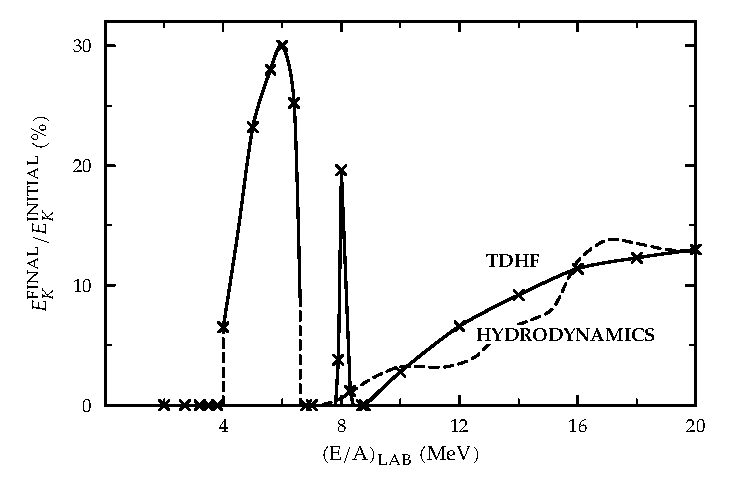
\includegraphics[width=0.8\textwidth]{pictures/12_4}
\par\end{centering}
\caption{\label{fig:12.4}两个核物质厚板碰撞中，末态平动动能与初态平动动能之比随 $E/A$ 的变化。零值表示聚变。（引自
\cite{BKN76}）虚线对应于 13.3.3 节中所讨论的流体力学计算。（引自 \cite{WMW77}）}
\end{figure}

厚板几何模型并不十分贴近现实，因为在 $x$ 和 $y$ 方向上的平移不变性阻止了核物质在碰撞过程中向侧面飞溅，并且高度的对称性削弱了阻尼机制。因此，二维
\cite{Ko76,CM76,MC76}、准三维 \cite{KDM77,MDK77} 以及全三维 \cite{CSM76,CMM78,BGK78,FW78}
计算相继被开展。这些计算需要耗费巨大的数值工作量，并给出了此类重离子散射过程中密度和流分布的清晰图像\footnote{关于重离子碰撞的导论，参见 \cite{NW76b}。}（见\ref{fig:12.5}）。

\begin{figure}[H]
\begin{centering}
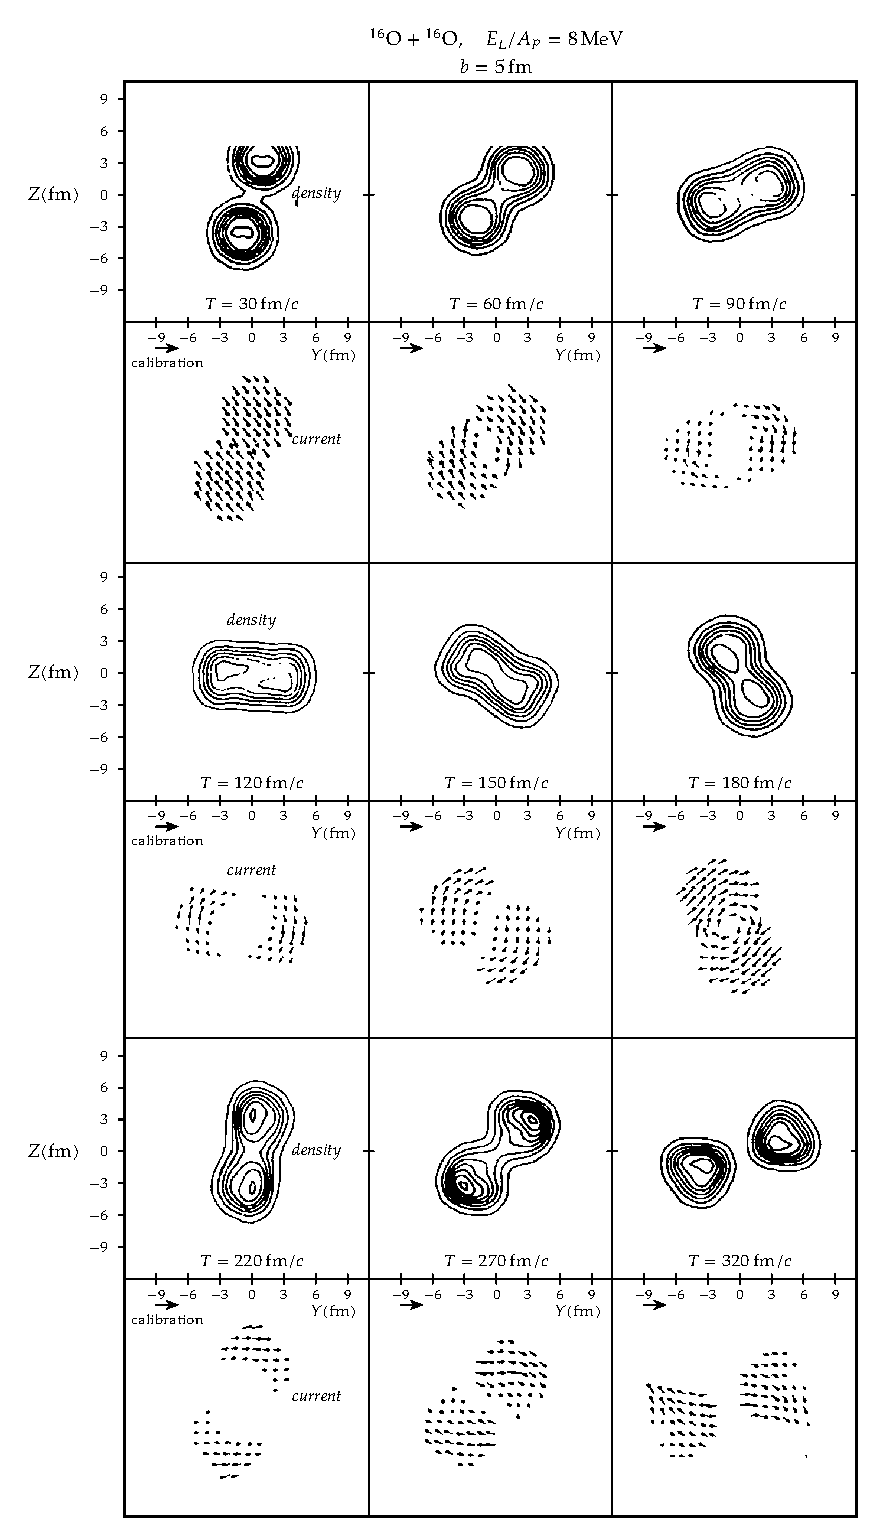
\includegraphics[width=0.85\textwidth]{pictures/12_5}
\par\end{centering}
\caption{\label{fig:12.5}在实验室参考系中，碰撞参数 $b=5\,\mathrm{fm}$ 时不同时刻 $T$ 下 $^{16}\mathrm{O}+{}^{16}\mathrm{O}$
碰撞的密度与速度分布。（引自 \cite{CMM78}）}
\end{figure}

TDHF 计算也被用于描述裂变过程 \cite{NKM78}。从极其接近鞍点处出发，系统演化一直被追踪至断裂为两个分离的碎片。然而在此我们不想进一步深入讨论利用
TDHF 理论所开展的大量数值计算细节。

\section{绝热时间相关Hartree-Fock理论（ATDHF）\label{sec:12.3}}

\subsection{ATDHF方程\label{subsec:12.3.1}}

正如我们在上一节所见，如今在某些情形下完全数值求解完整的 TDHF 方程是可能的。然而，对计算结果的解释却是困难的。因此，在本节中我们将研究一种作了进一步简化近似的理论：除了假定波函数在所有时刻都保持为
Slater 行列式（这构成了 TDHF 方法的特征）之外，我们仅考察缓慢过程并假设运动的速度很小。这一概念由 Belyaev \cite{Be65}
最早提出。其目标并非仅在于以某种近似求解 TDHF 方程 \ref{eq:12.9}，而是从中导出一个用于描述集体运动的 Bohr
型 Hamilton 量。正如我们将在 12.3.5.2 节所讨论的，对于诸如非简谐四极振动和低能重离子碰撞等多种集体运动，这一假设都是合理的；即使对于巨共振，绝热近似也是惊人地好的近似。

绝热近似有多种不同表述方式。最早的版本是由 Baranger 和 Kumar \cite{BK68} 在配对加四极力模型中引入的。后来，Baranger
和 Veneroni \cite{BV78}、Villars \cite{Vi75,Vi77}、Brink 等人 \cite{BEG76}
以及 Goeke 和 Reinhard \cite{GR78,RG78} 研究了更一般的形式体系。在这里，我们主要遵循 Baranger
和 Veneroni \cite{BV78} 的表述，因为在其中该理论的基本结构最为清晰；Villars 的方法将在 12.3.4
节中作更详细的探讨。结果表明，我们可以定义经典的坐标与正则共轭动量，它们服从经典的运动方程。

因此，首要问题在于定义这些坐标与动量。在 TDHF 理论中，一切均由单粒子密度 $\rho(t)$ 决定，而它在时间反演下并不是不变的。由于我们希望拥有时间反演不变的坐标，Baranger
和 Veneroni 提出了密度 $\rho(t)$ 的如下分解：

\begin{equation}
\rho(t)=\mathrm{e}^{\mathrm{i}\chi(t)/\hbar}\rho_{0}(t)\mathrm{e}^{-\mathrm{i}\chi(t)/\hbar}\label{eq:12.63}
\end{equation}

其中 $\rho_{0}$ 和 $\chi$ 都是 Hermitian 且在时间反演下为偶的矩阵，即：

\begin{equation}
\rho^{\dagger}_{0}=\rho_{0},\quad T\rho_{0}T^{-1}=\rho_{0};\qquad\chi^{\dagger}=\chi,\quad T\chi T^{-1}=\chi\label{eq:12.64}
\end{equation}

同样地，$\rho_{0}$ 满足 $\rho^{2}_{0}=\rho_{0}$，$\mathrm{Tr}\rho_{0}=N$，也就是说，它对应于一个
$N$ 维的 Slater 行列式 $|\Phi_{0}\rangle$。在下文中，$\rho_{0}$ 将作为坐标，并且正如我们将看到的，$\chi$
将作为动量。

相比于混合了时间反演偶分量与奇分量的 TDHF 密度 $\rho$，我们对以时间偶的行列式 $\rho_{0}$ 作为坐标要熟悉得多。例如在第
2 章中，我们使用了带有确定形变坐标 $q_{i}$ 的 Nilsson 函数，它们对应于时间偶的密度。对于带有时间偶约束的 CHF
计算（见 7.6 节），情况也是如此。

由 $\rho_{0}(t)$ 是时间偶的性质可得，与密度 $\rho_{0}(t)$ 相联系的总流密度在所有时刻均消失：

\begin{equation}
\boldsymbol{j}_{0}(\boldsymbol{r})=\mathrm{Tr}(\boldsymbol{j}\rho_{0})=0\label{eq:12.65}
\end{equation}

因为一个时间偶算符与一个时间奇算符乘积的迹必定为零，除非它是纯虚数。

因此在下文中，我们将 $\rho_{0}(t)$ 称为静态密度。它不应与与时间无关的密度相混淆，也不应与作为静态 HF 方程 $[h(\rho),\rho]=0$
之解的定态密度相混淆。然而结果表明，$\rho_{0}$ 是带有合适的（时间相关的）时间反演不变约束的静态 HF 方程的解 {[}见\ref{eq:12.120b}{]}。类似地，我们可以将
$\rho_{0}(t)$ 表示为：

\begin{equation}
\rho_{0}(t)=\mathrm{e}^{-\mathrm{i}\phi(t)/\hbar}\tilde{\rho}\mathrm{e}^{\mathrm{i}\phi(t)/\hbar}\label{eq:12.66}
\end{equation}

其中 $\phi(t)$ 是一个 Hermitian 时间奇算符，而 $\tilde{\rho}$ 是未受约束的静态 HF 问题
$[h(\tilde{\rho}),\tilde{\rho}]=0$ 的解。

在平移的情形下 {[}\ref{eq:12.32}{]}，我们已经见过密度 $\rho(t)$ 此类分解的一个范例，其中 $\chi$
为时间偶算符 $m\boldsymbol{v}\cdot\boldsymbol{r}$，而 $\phi$ 为时间奇算符 $t\boldsymbol{v}\cdot\boldsymbol{p}$。在转动的情形下
{[}\ref{eq:12.37}{]}，$(\boldsymbol{\omega}\cdot\boldsymbol{j})t$
是时间奇的，即它对应于算符 $\phi$。密度 $\tilde{\rho}$ 本身包含时间奇分量（见 7.7 节）且与时间无关。由于在此时不存在质心“角度”，在此情形下我们无法给出算符
$\chi$ 的显式表达式。\footnote{例如在 RPA 阶下，它已被计算为 Thouless-Valatin 方程 (8.106) 的解 $\Theta$。}

在下文中，我们将仅使用分解\ref{eq:12.63}。可以证明（见附录 D.2 节），在如下条件下该分解是唯一的：

(i) $\chi$ 的全部本征值 $\chi_{i}$ 满足：

\begin{equation}
-\frac{\pi\hbar}{2}<\chi_{i}\leqslant\frac{\pi\hbar}{2}\label{eq:12.67a}
\end{equation}

(ii) 在 $\rho_{0}$ 呈对角形式的基底中，$\chi$ 的 pp 和 hh 矩阵元消失，即：

\begin{equation}
\chi^{hh}=\rho_{0}\chi\rho_{0}=0;\qquad\chi^{pp}=\sigma_{0}\chi\sigma_{0}=0\label{eq:12.67b}
\end{equation}

这里我们利用了如下事实：在 $\rho_{0}$ 对角化的基底下，$\rho_{0}$ 是空穴态上的投影算符，而 $\sigma_{0}=1-\rho_{0}$
是粒子态上的投影算符。在下文中，我们将始终在该基底中展开。然而应当注意，由于 $\rho_{0}(t)$ 是时间的函数，该基底依赖于时间。

我们可能会问条件 \ref{eq:12.67a} 与 \ref{eq:12.67b} 是否是必要的。事实上并非如此；这仅仅是一个相当自然的选择，\footnote{然而已有研究表明，这一选择与假设 $\chi$ 在坐标空间中局域 \cite{BQ78} 是不相容的；有时局域的 $\chi$
似乎是自然的选择，正像我们在平移情形 {[}式 (12.32){]} 中所见的那样。}因为 pp 和 hh 矩阵元扮演着非常重要的角色。Baranger 和 Veneroni \cite{BV78} 已经证明，具有非零矩阵元
$\chi^{pp}$ 和 $\chi^{hh}$ 的任何其他分解所给出的结果，与我们在下文导出的结果之间的偏差，其阶数在 ATDHF
方法中本来就是被忽略的 $\chi$ 的高阶项。因此采用条件 \ref{eq:12.67a} 与 \ref{eq:12.67b}
与该近似是一致的，我们在下文中将采纳这些条件。

绝热近似现在体现为假设系统的密度 $\rho(t)$ 在所有时刻都接近于密度 $\rho_{0}(t)$，也就是说，我们在所有时刻都拥有一个近乎静态的密度。换言之，这意味着引入时间奇分量的矩阵
$\chi$ 是微小的。对于 TDHF 方程的所有解 $\rho(t)$ 而言这当然并不普遍成立，但我们仅仅对满足这一条件的解感兴趣。因此我们可以将
$\rho(t)$ 展开到 $\chi$ 的二阶：

\begin{equation}
\rho=\mathrm{e}^{\mathrm{i}\chi/\hbar}\rho_{0}\mathrm{e}^{-\mathrm{i}\chi/\hbar}\simeq\rho_{0}+\rho_{1}+\rho_{2}\label{eq:12.68}
\end{equation}

其中：

\begin{equation}
\rho_{1}=\frac{\mathrm{i}}{\hbar}[\chi,\rho_{0}],\qquad\chi=-\mathrm{i}\hbar[\rho_{1},\rho_{0}]\label{eq:12.69}
\end{equation}

\begin{equation}
\rho_{2}=-\frac{1}{2\hbar^{2}}[\chi,[\chi,\rho_{0}]]=\frac{1}{\hbar^{2}}\left(\chi\rho_{0}\chi-\frac{1}{2}(\chi^{2}\rho_{0}+\rho_{0}\chi^{2})\right)\label{eq:12.70}
\end{equation}

式 $(\text{D}.32)$ 表明 $\rho_{1}$ 仅具有 ph 和 hp 矩阵元，而 $\rho_{2}$ 仅具有
pp 和 hh 矩阵元：

\begin{equation}
\rho_{1}=\frac{\mathrm{i}}{\hbar}(\sigma_{0}\chi\rho_{0}-\rho_{0}\chi\sigma_{0})\label{eq:12.71}
\end{equation}

\begin{equation}
\rho_{2}=\frac{1}{\hbar^{2}}\left(\sigma_{0}\chi\rho_{0}\chi\sigma_{0}-\rho_{0}\chi\sigma_{0}\chi\rho_{0}\right)\label{eq:12.72}
\end{equation}

以完全相同的方式，我们可以展开\footnote{缩写符号 $\mathrm{Tr}_{1}$ 的定义见式 (E.19)。}：

\begin{equation}
h(\rho)=t+\mathrm{Tr}_{1}(\bar{v}\rho)=h_{0}+\Gamma_{1}+\Gamma_{2}\label{eq:12.73}
\end{equation}

其中：

\begin{equation}
h_{0}=t+\mathrm{Tr}_{1}(\bar{v}\rho_{0}),\qquad\Gamma_{1}=\mathrm{Tr}_{1}(\bar{v}\rho_{1}),\qquad\Gamma_{2}=\mathrm{Tr}_{1}(\bar{v}\rho_{2})\label{eq:12.74}
\end{equation}

在 $\rho$ 和 $h$ 的展开式中，偶数阶项在时间反演下总是偶的，而奇数阶项在时间反演下总是奇的。

如果我们将展开\ref{eq:12.68} 和 \ref{eq:12.73} 代入 TDHF 方程 \ref{eq:12.9}，我们可以根据它们在时间反演下的行为将其分解，从而得到两个
ATDHF 方程：

\begin{align}
(\mathrm{I})\qquad\mathrm{i}\hbar\dot{\rho}_{0} & =[h_{0},\rho_{1}]+[\Gamma_{1},\rho_{0}]\label{eq:12.75a}\\
(\mathrm{II})\qquad\mathrm{i}\hbar\dot{\rho}_{1} & =[h_{0},\rho_{0}]+[\Gamma_{1},\rho_{1}]+[\Gamma_{2},\rho_{0}]\label{eq:12.75b}
\end{align}

正如我们稍后将看到的，这两个方程仅有 ph 和 hp 部分是重要的。在导出这些方程时，我们忽略了 $\chi$ 的更高阶项。为了能够做到这一点，我们必须知道时间导数
$\dot{\rho}_{0},\dot{\rho}_{1},\dot{\rho}_{2}\dots$ 关于 $\chi$ 的阶数。在
Fourier 分析中，它们带有一个因子 $\omega$，其中 $\omega$ 为相应的频率。现在我们必须区分大振幅运动与小振幅振荡。在大振幅情形下，$\omega$
必须具有 $\chi$ 的数量级且微小；正如我们已经看到的，这意味着 $\dot{\rho}_{i}$ 比 $\rho_{i}$
在 $\chi$ 上高出一阶。在小振幅情形下，$\omega$ 并不必然与 $\chi$ 具有相同阶数，即 $\dot{\rho}_{i}$
与 $\rho_{i}$ 在 $\chi$ 上具有相同阶数。

因此在上述方程 (I) 中，我们略去了所有等于或高于二阶的项；在方程 (II) 中，我们略去了所有等于或高于三阶的项。此外，在方程
(II) 中略去了 $[h_{0},\rho_{2}]$ 项，其原因我们稍后将讨论。

在 $\chi$ 的零阶下，我们得到静态情形：

\begin{equation}
\dot{\rho}_{0}=0,\qquad[h_{0},\rho_{0}]=0\label{eq:12.76}
\end{equation}

因此方程 (I) 和 (II) 始终计入了关于 $\chi$ 的第一个非平凡阶次。特别地，这表明在大振幅情形下（其中 $\dot{\rho}_{1}$
为 $\chi$ 的二阶量），\ref{eq:12.75b} 中的 $[h_{0},\rho_{0}]$ 项也至少为二阶量，尽管
$h_{0}$ 与 $\rho_{0}$ 各自单独来看都是很大的量。这意味着静态 HF 方程 \ref{eq:12.76} 几乎被满足。原子核在所有时刻都几乎处于静态平衡状态，且运动是缓慢的。

正如我们将在 12.3.2 节中详细看到的，我们可以对 ATDHF 方程赋予经典诠释，其中 $\rho_{0}$ 和 $\chi$
是正则共轭的坐标和动量。方程 (I) 给出了速度 $\dot{\rho}_{0}$ 与动量 $\chi$ 之间的线性联系。相应的质量张量取决于坐标
$\rho_{0}$ 并依赖于时间。方程 (II) 在左端具有动量的时间导数。因此右端代表一个力。它依赖于 $[h_{0},\rho_{0}]$
项以及动量 $\chi$ 的二次项。从零速度下的某个初始值 $\rho_{0}$ 出发，$[h_{0},\rho_{0}]$
因此是在初始时刻加速系统的力。由于动量在所有时刻保持微小，$[h_{0},\rho_{0}]$ 在所有时刻的微小性因而是绝热运动存在的一个充要条件。如果在时间偶密度
$\rho_{0}$ 的空间中存在一个 $[h_{0},\rho_{0}]$ 微小的完整区域，那么我们便可以在该区域内找到一条对应于绝热运动的轨迹
$\rho(t)$。

我们仍须说明方程 (I) 和 (II) 应当仅在 ph 和 hp 空间中使用：方程 (I) 的 pp 和 hh 矩阵元至少为 $\chi$
的二阶量。例如，由式 $(\text{D}.32)$ 可知 $\dot{\rho}_{0}$ 仅具有 ph 和 hp 矩阵元，且由\ref{eq:12.71}
可知对 $\rho_{1}$ 也是如此。因此方程 (I) 右端的唯一非零 hh 矩阵元为：

\begin{equation}
\rho_{0}[h_{0},\rho_{1}]\rho_{0}=-\rho_{0}\left([h_{0},\rho_{0}]\rho_{1}+\rho_{1}[h_{0},\rho_{0}]\right)\rho_{0}\label{eq:12.77}
\end{equation}

它至少为二阶量，因为在大振幅情形下 $[h_{0},\rho_{0}]$ 为二阶量，而在小振幅情形下为一阶量。对于方程 (I) 的
pp 矩阵元，结论同样成立。

在方程 (II) 中，我们略去了 $[h_{0},\rho_{2}]$ 项。由\ref{eq:12.72} 可见，$\rho_{2}$
仅具有 hh 和 pp 矩阵元。因此 $[h_{0},\rho_{2}]$ 的 ph 矩阵元仅包含 $h_{0}$ 的 ph 和
hp 矩阵元，它们关于 $\chi$ 至少为一阶量。所以，在方程 (II) 的 hp 和 ph 部分中 $[h_{0},\rho_{2}]$
可以被忽略。在方程 (II) 的 hh 和 pp 部分中我们不能再忽略该项，因为 $h_{0}$ 的 pp 和 hh 矩阵元很大。然而我们可以证明，计入了
$[h_{0},\rho_{2}]$ 项的方程 (II) 的 pp 和 hh 矩阵元恒等于零。这需要较长的推导 \cite{BV78}；在此我们仅给出最重要的步骤。首先我们由\ref{eq:12.72}
表示 $\rho_{2}$；然后利用\ref{eq:12.71} 并得到 $\dot{\rho}_{1}$ 的 hh 矩阵元：

\begin{equation}
\rho_{0}\dot{\rho}_{1}\rho_{0}=-\dot{\rho}_{0}\rho_{1}\rho_{0}+\rho_{0}\rho_{1}\dot{\rho}_{0}\label{eq:12.78}
\end{equation}

最后，代入方程 (I) 对 $\dot{\rho}_{0}$ 的表达式，我们发现方程 (II) 的 pp 和 hh 部分恒消失。

如果我们从某些初始值 $\rho_{0}(0),\rho_{1}(0)$ 或者 $\rho_{0}(0)$ 和 $\dot{\rho}_{0}(0)$
出发，ATDHF 方程组 \ref{eq:12.75a} 与 \ref{eq:12.75b} 允许我们在所有时刻计算 $\rho_{0}(t)$
和 $\rho_{1}(t)$。然而，这一问题的求解至少与精确 TDHF 方程一样困难，在实践中没有人会这样做。绝热理论的主要优势在于：它允许我们导出一个用于描述集体运动的经典
Hamilton 量。

\subsection{集体Hamilton量\label{subsec:12.3.2}}

我们现在能够用变量 $\rho_{0}$ 和 $\rho_{1}$（或 $\rho_{0}$ 和 $\chi$）来表达系统的总能量
$E$。由式 $(5.28)$，我们求得：

\begin{equation}
E=\mathrm{Tr}(t\rho)+\frac{1}{2}\mathrm{Tr}_{1}\mathrm{Tr}_{2}(\rho\bar{v}\rho)=\mathcal{K}+\mathcal{V}\label{eq:12.79}
\end{equation}

其中我们将所有依赖于速度二阶的项归入动能 $\mathcal{K}$ 中，并将所有仅包含静态密度 $\rho_{0}$ 的项归入势能
$\mathcal{V}$ 中。由于 Hamilton 量的时间反演不变性，关于 $\rho_{1}$ 的线性项消失。我们求得
$\mathcal{V}$ 为密度分布 $\rho_{0}$ 的静态 HF 能量：

\begin{equation}
\mathcal{V}=\mathrm{Tr}(t\rho_{0})+\frac{1}{2}\mathrm{Tr}_{1}\mathrm{Tr}_{2}(\rho_{0}\bar{v}\rho_{0})\label{eq:12.80}
\end{equation}

动能具有如下形式：

\begin{equation}
\mathcal{K}=\mathrm{Tr}(h_{0}\rho_{2})+\frac{1}{2}\mathrm{Tr}_{1}\mathrm{Tr}_{2}(\rho_{1}\bar{v}\rho_{1})\label{eq:12.81}
\end{equation}

它二次方地依赖于 $\rho_{1}$（或 $\chi$），并且由于\ref{eq:12.75a}，也二次方地依赖于速度 $\dot{\rho}_{0}$。我们可以用几种方式来书写它。首先，我们采用使得
$h_{0}$ 的 pp 部分与 hh 部分均对角化的基底。这总是可行的，因为 $\rho_{0}$ 在这种变换下保持不变。我们将本征值记为
$\epsilon_{m}$（粒子）和 $\epsilon_{i}$（空穴）。利用\ref{eq:12.69} 以及定义：

\begin{align}
A_{minj} & =(\epsilon_{m}-\epsilon_{i})\delta_{nm}\delta_{ij}+\bar{v}_{mjin}\nonumber \\
B_{minj} & =\bar{v}_{mnij}\label{eq:12.82}
\end{align}

利用 $\chi_{im}=\chi^{*}_{mi}$，我们求得：

\begin{equation}
\mathcal{K}=\frac{1}{2\hbar^{2}}(\chi^{*},\chi)\left(\begin{array}{cc}
A & B\\
B^{*} & A^{*}
\end{array}\right)\left(\begin{array}{c}
\chi\\
\chi^{*}
\end{array}\right)\label{eq:12.83}
\end{equation}

其中在 $(\chi_{mi},\chi^{*}_{mi})$ 中矩阵的指标遍历所有 ph 对 $(mi)$。它看起来与第 8
章中的 RPA 记号非常相似。然而它更为普遍，因为单粒子能量与 $\chi$ 都依赖于时间。

我们也可以在这种记号下书写 ATDHF 方程 (I)：

\begin{equation}
\hbar\left(\begin{array}{c}
\dot{\rho}_{0}\\
-\dot{\rho}^{*}_{0}
\end{array}\right)=\left(\begin{array}{cc}
A & B\\
B^{*} & A^{*}
\end{array}\right)\left(\begin{array}{c}
\chi\\
\chi^{*}
\end{array}\right)\label{eq:12.84}
\end{equation}

它联系了速度与动量，并表明矩阵：

\begin{equation}
\mathfrak{M}=\hbar^{2}\left(\begin{array}{cc}
A & B\\
B^{*} & A^{*}
\end{array}\right)^{-1}\label{eq:12.85}
\end{equation}

代表一个依赖于坐标 $\rho_{0}$ 的质量张量。容易看出，在转动情形下它对应于转动惯量的 Thouless-Valatin
值 $(8.142)$。动能\ref{eq:12.83} 具有形式：

\begin{equation}
\mathcal{K}=\frac{1}{2}(\dot{\rho}^{*}_{0},-\dot{\rho}_{0})\mathfrak{M}\left(\begin{array}{c}
\dot{\rho}_{0}\\
-\dot{\rho}^{*}_{0}
\end{array}\right)\label{eq:12.86}
\end{equation}

我们因此导出了一个经典的 Hamilton 函数，它依赖于坐标 $\rho_{0}$ 并二次方地依赖于动量 $\chi$：

\begin{equation}
\mathcal{H}(\chi,\rho_{0})=\frac{1}{2\hbar^{2}}(\chi^{*},\chi)\mathfrak{M}^{-1}\left(\begin{array}{c}
\chi\\
\chi^{*}
\end{array}\right)+\mathcal{V}(\rho_{0})\label{eq:12.87}
\end{equation}

$\mathcal{V}(\rho_{0})=\langle\Phi|H|\Phi\rangle$ 是完整 Hamilton 量在静态波函数
$|\Phi\rangle$ 下的期望值。动能完全源自波函数的时间奇分量。正如我们从\ref{eq:12.81} 所见，它由两项贡献组成。第一项包含静态势
$h_{0}$，第二项包含由于时间奇密度分量 $\rho_{1}$ 引起的自洽势重整化效应。如果我们略去自洽场的这一重整化效应（例如在唯象势中），质量张量
\ref{eq:12.85} 中的矩阵 $B$ 将消失，我们将获得 Inglis 公式（参见 8.4.7 节）。

为了使形式体系完备，我们必须说明可以从 Hamilton 变分原理得到 ATDHF 方程。对固定的 $\rho_{0}$，我们求得：

\begin{equation}
\frac{\partial\mathcal{H}}{\partial\chi^{*}}=\frac{1}{\hbar^{2}}\mathfrak{M}^{-1}\left(\begin{array}{c}
\chi\\
\chi^{*}
\end{array}\right)=\dot{\rho}_{0}\label{eq:12.88}
\end{equation}

这表明第一个 ATDHF 方程 {[}对应于\ref{eq:12.84}{]} 与 Hamilton 方程 $\dot{q}=\partial\mathcal{H}/\partial p$
完全等价。第二个 ATDHF 方程的推导更为复杂。我们首先计算由改变 $\delta\rho_{0}$ 所引起的 $\rho_{1}$
和 $\rho_{2}$ 的变化。对固定的 $\chi$，由\ref{eq:12.69} 和 \ref{eq:12.70}
可得：

\begin{equation}
\delta\rho_{1}=\frac{\mathrm{i}}{\hbar}[\chi,\delta\rho_{0}],\qquad\delta\rho_{2}=-\frac{1}{2\hbar^{2}}[\chi,[\chi,\delta\rho_{0}]]\label{eq:12.89}
\end{equation}

因此能量 \ref{eq:12.79} 的改变量为：

\begin{equation}
\delta E=\mathrm{Tr}(\Gamma_{2}\delta\rho_{0}+\Gamma_{1}\delta\rho_{1}+h_{0}\delta\rho_{2})+\delta\mathcal{V}\label{eq:12.90}
\end{equation}

由于 $\chi$ 和 $\delta\rho_{0}$ 仅有 ph 和 hp 矩阵元，$h_{0}$ 对这些迹有贡献的唯一矩阵元是
ph 和 hp 矩阵元。正如在上一小节中所讨论的，它们关于 $\chi$ 至少为一阶量。为了保持自洽，我们因此必须略去\ref{eq:12.90}
中的最后一项，并求得第二个 Hamilton 方程：

\begin{equation}
-\dot{\chi}=\frac{\partial\mathcal{H}}{\partial\rho_{0}}=\frac{\partial\mathcal{K}}{\partial\rho_{0}}+\frac{\partial\mathcal{V}}{\partial\rho_{0}}\label{eq:12.91}
\end{equation}

当然，我们只需使用这些方程的 ph 和 hp 矩阵元。结合：

\begin{equation}
\rho_{0}\dot{\rho}_{1}\rho_{0}=-\frac{\mathrm{i}}{\hbar}\dot{\chi}\label{eq:12.92}
\end{equation}

以及静态能量对密度 $\rho_{0}$ 的微商 $\partial\mathcal{V}/\partial\rho_{0}$
给出了 $h_{0}$ 的 ph 矩阵元 {[}见式 $(5.32)${]} 的事实，我们看到\ref{eq:12.91} 精确对应于第二个
ATDHF 方程 \ref{eq:12.75b}。

因此，第二个 ATDHF 方程描述了系统的加速度。除了静态力 $(\partial\mathcal{V}/\partial\rho_{0})$
之外，还存在源于质量张量 \ref{eq:12.85} 对坐标的依赖性的附加项。

利用 Hamilton 形式体系，我们现已建立了与经典系统的完全类比。我们也可以利用 Lagrange 形式体系来完成这一点 \cite{BV78}。

在小振幅极限下，我们可以用一种不同于通常方式（见 8.4 节）的方法导出 RPA。我们假设 $\rho_{0}(t)$ 保持接近于静态
HF 问题 $[h(\tilde{\rho}),\tilde{\rho}]=0$ 的定态解 $\tilde{\rho}$：

\begin{equation}
\rho_{0}(t)=\tilde{\rho}+\xi(t)\label{eq:12.93}
\end{equation}

并将势能 $\mathcal{V}(\rho_{0})$ 在点 $\tilde{\rho}$ 处展开至二阶 {[}见式 $(7.34)${]}：

\begin{equation}
\mathcal{V}(\rho_{0})=\mathcal{V}(\tilde{\rho})+\frac{1}{2}(\xi^{*},\xi)\mathfrak{S}\left(\begin{array}{c}
\xi\\
\xi^{*}
\end{array}\right)\label{eq:12.94}
\end{equation}

利用稳定性矩阵 $\mathfrak{S}$ {[}式 $(7.37)${]}（曲率张量），我们得到能量：

\begin{equation}
\mathcal{H}=\frac{1}{2\hbar^{2}}(\chi^{*},\chi)\mathfrak{M}^{-1}\left(\begin{array}{c}
\chi\\
\chi^{*}
\end{array}\right)+\frac{1}{2}(\xi^{*},\xi)\mathfrak{S}\left(\begin{array}{c}
\xi\\
\xi^{*}
\end{array}\right)\label{eq:12.95}
\end{equation}

这是耦合谐振子的 Hamilton 函数。相应的运动方程由频率为 $\Omega$ 的简谐振动求解，我们最终得到本征值问题 \cite{Go59}：

\begin{equation}
\mathfrak{M}\Omega^{2}\mathfrak{X}=\mathfrak{S}\mathfrak{X}\label{eq:12.96}
\end{equation}

频率 $(\hbar\Omega)$ 是矩阵：

\begin{equation}
\left(\begin{array}{cc}
A & B\\
-B^{*} & -A^{*}
\end{array}\right)=\sigma_{3}\mathfrak{M}^{-1},\qquad\sigma_{3}=\left(\begin{array}{cc}
1 & 0\\
0 & -1
\end{array}\right)\label{eq:12.97}
\end{equation}

的本征值。它们可以通过仅对 $\mathfrak{M}^{-1}\mathfrak{S}$ 进行对角化来求得，这正是 RPA 矩阵。这之所以可能，仅仅是因为质量张量
$\mathfrak{M}$ 的逆矩阵具有与曲率张量 $\mathfrak{S}$ 类似的结构。

\subsection{约化为少数集体坐标\label{subsec:12.3.3}}

我们回到大振幅问题。ATDHF 方程组 \ref{eq:12.75a} 与 \ref{eq:12.75b} 仍包含所有自由度，对于实际应用而言过于普遍。特别地，它并不比完整的
TDHF 方程 \ref{eq:12.9} 更易求解；然而，绝热近似也仅对少数轨道有效。因此，大幅度减少自由度的数目应当是可能的。

选择合适的集体变量当然是一个重大问题。在深入讨论此问题之前，我们首先假设已经实现了这种约化，并拥有一个时间偶的 Slater 行列式族：

\begin{equation}
|\Phi(\boldsymbol{q})\rangle=|\Phi(q_{1}\dots q_{f})\rangle\label{eq:12.98}
\end{equation}

以及相应的密度 $\rho_{0}(\boldsymbol{q})$，它们具有如下性质：ATDHF 问题的解将始终保持在由实参数
$\boldsymbol{q}$ 所表征的该 Slater 行列式子集之内；即存在一条路径 $\boldsymbol{q}(t)$
满足：

\begin{equation}
\rho_{0}(t)=\rho_{0}(\boldsymbol{q}(t))\label{eq:12.99}
\end{equation}

由此我们求得速度：

\begin{equation}
\dot{\rho}_{0}=\sum^{f}_{\mu=1}\dot{q}_{\mu}\frac{\partial\rho_{0}}{\partial q_{\mu}}\label{eq:12.100}
\end{equation}

正如在附录 D.3 节中所展示的，Hermitian 矩阵 $\partial\rho_{0}/\partial q_{\mu}$
在 $\rho_{0}$ 为对角的基底下仅具有 ph 和 hp 矩阵元，且等于厄米单粒子算符 $\hat{\boldsymbol{P}}=(\hat{P}_{1},\dots,\hat{P}_{f})$
的相应矩阵元\footnote{这些矩阵对应于式 (12.32) 中的矩阵 $p$。我们在此使用大写字母 $P$ 以区别于集体动量 $p$ {[}式 (12.104){]}。}。单粒子矩阵
$\boldsymbol{P}$ 具有矩阵元 {[}见式 (D.36) 及以下{]}：

\begin{equation}
\boldsymbol{P}_{mi}=\boldsymbol{P}^{*}_{im}=-\langle m|\frac{\hbar}{\mathrm{i}}\frac{\partial}{\partial\boldsymbol{q}}|i\rangle;\qquad\boldsymbol{P}_{mm^{\prime}}=\boldsymbol{P}_{ii^{\prime}}=0\label{eq:12.101}
\end{equation}

在 $\rho_{0}$ 对角化的基底下。

既然我们现在有了速度 $\dot{\rho}_{0}$ 关于 $\dot{\boldsymbol{q}}$ 的显式表达式，由\ref{eq:12.86}
和 \ref{eq:12.100}，我们得到动能：

\begin{equation}
\mathcal{K}=\frac{1}{2}\sum^{f}_{\mu,\mu^{\prime}=1}M_{\mu\mu^{\prime}}(\boldsymbol{q})\dot{q}_{\mu}\dot{q}_{\mu^{\prime}}\label{eq:12.102}
\end{equation}

以及实的集体质量张量：

\begin{equation}
M_{\mu\mu^{\prime}}(\boldsymbol{q})=\frac{1}{\hbar^{2}}(P^{*}-P)_{\mu}\mathfrak{M}\left(\begin{array}{c}
P\\
-P^{*}
\end{array}\right)_{\mu^{\prime}}\label{eq:12.103}
\end{equation}

我们还可以定义集体动量 $p_{\mu}$，并由\ref{eq:12.84} 和 \ref{eq:12.100} 求得：

\begin{equation}
p_{\mu}=\sum_{\mu^{\prime}}M_{\mu\mu^{\prime}}(\boldsymbol{q})\dot{q}_{\mu^{\prime}}=\mathrm{Tr}\left(\chi\frac{\partial\rho_{0}}{\partial q_{\mu}}\right)=\mathrm{Tr}\left(\chi\frac{\partial}{\partial q_{\mu}}\rho_{0}\right)\label{eq:12.104}
\end{equation}

能量呈现出经典 Hamilton 函数的形式：

\begin{equation}
\mathcal{H}(\boldsymbol{p},\boldsymbol{q})=\frac{1}{2}\sum_{\mu\mu^{\prime}}M^{-1}_{\mu\mu^{\prime}}(\boldsymbol{q})p_{\mu}p_{\mu^{\prime}}+\mathcal{V}(\boldsymbol{q})\label{eq:12.105}
\end{equation}

为了证明我们真正拥有一个正则系统，我们必须验证从函数 \ref{eq:12.105} 导出的 Hamilton 方程。第一个方程由下式直接给出：

\begin{equation}
\frac{\partial\mathcal{H}}{\partial p_{\mu}}=\sum_{\mu^{\prime}}M^{-1}_{\mu\mu^{\prime}}p_{\mu^{\prime}}=\dot{q}_{\mu}\label{eq:12.106}
\end{equation}

在第二个方程的情形下，利用\ref{eq:12.87}、\ref{eq:12.90} 和 \ref{eq:12.104}，并在一种显然的简记符号
\cite{BGV76} 下，我们得到：

\begin{align}
\frac{\partial\mathcal{H}}{\partial q_{\mu}} & =\frac{\partial E}{\partial\rho^{*}_{0}}\frac{\partial\rho_{0}}{\partial q_{\mu}}+\frac{\partial E}{\partial\chi^{*}}\frac{\partial\chi}{\partial q_{\mu}}=-\dot{\chi}\frac{\partial\rho_{0}}{\partial q_{\mu}}+\dot{\rho}_{0}\frac{\partial\chi}{\partial q_{\mu}}\nonumber \\
 & =-\dot{\chi}\frac{\partial\rho_{0}}{\partial q_{\mu}}-\chi\frac{\mathrm{d}}{\mathrm{d}t}\frac{\partial\rho_{0}}{\partial q_{\mu}}+\sum_{\mu^{\prime}}\dot{q}_{\mu^{\prime}}\frac{\partial}{\partial q_{\mu}}\left(\chi\frac{\partial}{\partial q_{\mu^{\prime}}}\rho_{0}\right)\nonumber \\
 & =-\frac{\mathrm{d}}{\mathrm{d}t}\left(\chi\frac{\partial\rho_{0}}{\partial q_{\mu}}\right)+\sum_{\mu^{\prime}}\dot{q}_{\mu^{\prime}}\frac{\partial}{\partial q_{\mu}}p_{\mu^{\prime}}\nonumber \\
 & =-\frac{\mathrm{d}}{\mathrm{d}t}p_{\mu}\label{eq:12.107}
\end{align}

因为 $p_{\mu}$ 和 $q_{\mu}$ 是独立变量 $[(\partial/\partial q_{\mu})p_{\mu^{\prime}}=0]$。

人们还经常引入一组仅具有 ph 和 hp 矩阵元的 Hermitian 算符 $\hat{\boldsymbol{Q}}$，其定义为：

\begin{equation}
\left(\begin{array}{c}
Q\\
Q^{*}
\end{array}\right)_{\mu}=\frac{\hbar}{\mathrm{i}}\sum_{\mu^{\prime}}M^{-1}_{\mu\mu^{\prime}}\left(\begin{array}{cc}
A & -B\\
-B^{*} & A^{*}
\end{array}\right)^{-1}\left(\begin{array}{c}
P\\
-P^{*}
\end{array}\right)_{\mu^{\prime}}\label{eq:12.108}
\end{equation}

它们与算符 $\chi$ 密切相关：

\begin{equation}
\chi=\sum_{\mu}p_{\mu}Q_{\mu}\label{eq:12.109}
\end{equation}

质量张量 \ref{eq:12.103} 也可以表示为：

\begin{equation}
M_{\mu\mu^{\prime}}(\boldsymbol{q})=(Q^{*},Q)_{\mu}\left(\begin{array}{cc}
A & B\\
B^{*} & A^{*}
\end{array}\right)\left(\begin{array}{c}
Q\\
Q^{*}
\end{array}\right)_{\mu^{\prime}}\label{eq:12.110}
\end{equation}

算符 $\hat{\boldsymbol{P}}$ 和 $\hat{\boldsymbol{Q}}$ 服从归一化条件：

\begin{equation}
\langle\Phi_{0}|[\hat{P}_{\mu},\hat{Q}_{\mu^{\prime}}]|\Phi_{0}\rangle=\mathrm{Tr}(\rho_{0}[P_{\mu},Q_{\mu^{\prime}}])=\frac{\hbar}{\mathrm{i}}\delta_{\mu\mu^{\prime}}\label{eq:12.111}
\end{equation}

由于 $\boldsymbol{P}$ 仅具有 ph 和 hp 矩阵元，算符 $\hat{\boldsymbol{P}}$ 由\ref{eq:12.101}
唯一确定。它完全由静态波函数族 $|\Phi_{0}(\boldsymbol{q})\rangle$ 所给出。如果我们已知“动量”
$\boldsymbol{p}$ {[}\ref{eq:12.104}{]} 以及“坐标” $\boldsymbol{q}$，我们便获得时间相关的
Slater 行列式：

\begin{equation}
|\Phi(\boldsymbol{p},\boldsymbol{q})\rangle=\mathrm{e}^{\mathrm{i}\sum_{\mu}p_{\mu}\hat{Q}_{\mu}/\hbar}|\Phi_{0}(\boldsymbol{q})\rangle\label{eq:12.112}
\end{equation}

如果我们将动量 $\boldsymbol{p}$ 视为一个微分算符 $(\hbar/\mathrm{i})\partial/\partial\boldsymbol{q}$，这在某种意义上看起来像一个
Taylor 展开，但事实并非如此，因为 $\hat{\boldsymbol{Q}}$ 依赖于 $\boldsymbol{q}$，且
$\hat{\boldsymbol{Q}}$ 与 $\hat{\boldsymbol{P}}$ 并不对易。只有在微小 $\boldsymbol{p}$
的极限下，由\ref{eq:12.111} 我们才能导出：

\begin{equation}
|\Phi(\boldsymbol{p},\boldsymbol{q})\rangle\simeq\left(1+\sum_{\mu}p_{\mu}\frac{\partial}{\partial p_{\mu}}\right)|\Phi(\boldsymbol{p}=0,\boldsymbol{q})\rangle\label{eq:12.113}
\end{equation}

该理论的一个范例（其中 $\hat{\boldsymbol{P}}$ 和 $\hat{\boldsymbol{Q}}$ 是精确的常数算符）由
Galilei 变换给出 {[}见\ref{eq:12.32}{]}。

\subsection{集体坐标的选取\label{subsec:12.3.4}}

在导出 Hamilton 量 \ref{eq:12.105} 时，我们假设我们已经能够找到一个静态行列式族 $|\Phi_{0}(\boldsymbol{q})\rangle$，具有如下性质：在某些初始条件下
ATDHF 方程 \ref{eq:12.75a} 与 \ref{eq:12.75b} 的解对应于贯穿该子集的一条轨道。在一般情形下，此类子集将仅包含单一的一维轨道。然而在某些情况下，也可以找到高维超曲面，使得
ATDHF 问题 \ref{eq:12.75a} 与 \ref{eq:12.75b} 的解对于许多不同的初始条件均保持在该子集之内。例如，这在转动情形下是显然成立的，此时超曲面由
Euler 角所参数化。

在导出集体 Hamilton 量 \ref{eq:12.105} 时，我们假设我们已经选定了该子集 $\rho_{0}(\boldsymbol{q})$。然后，我们仅使用了第一个
ATDHF 方程 \ref{eq:12.75a} 来计算相应的动量与惯性参数。第二个方程 \ref{eq:12.75b} 仅被用于导出经典运动方程
\ref{eq:12.107}。我们根本没有考察它是否被给定的路径 $\rho_{0}(\boldsymbol{q})$ 所满足。事实上，在一般情形下它并不会被满足。在
12.3.1 节中我们看到，为了满足第二个 ATDHF 方程，我们至少必须要求：

\begin{equation}
[h_{0}(\rho_{0}),\rho_{0}]=\mathcal{O}(\chi^{2})\label{eq:12.114}
\end{equation}

这并不是对所有路径都自动成立的。如果我们在 $\rho_{0}$ 的空间中任意选取一条路径，沿着该路径计算质量参数与势能并求解经典运动方程
\ref{eq:12.106} 和 \ref{eq:12.107}，那么该解一般而言并不构成 ATDHF 方程 \ref{eq:12.75a}
与 \ref{eq:12.75b} 的解。Villars \cite{Vi75,Vi77} 利用第二个方程来确定最优路径 $\rho_{0}(q)$。为简便起见，我们在下文中局限于单一集体坐标
$q$。

正如我们在 12.3.1 节所指出的，该方程仅有 ph 和 hp 部分是有意义的。利用\ref{eq:12.69}，它可以写为：

\begin{equation}
\dot{\chi}=-[h_{0},\rho_{0}]-[\Gamma_{1},\rho_{1}]-[\Gamma_{2},\rho_{0}]\label{eq:12.115}
\end{equation}

由于 $[h_{0},\rho_{0}]$ 具有时间偶性且仅有 ph 和 hp 矩阵元，我们可以将其写为某个时间偶 Hermitian
单粒子算符 $F$ 与 $\rho_{0}$ 的对易子：

\begin{equation}
[h_{0},\rho_{0}]=[F,\rho_{0}]\label{eq:12.116}
\end{equation}

我们假设已知第一个 ATDHF 方程的解 $\chi$ 并使用\ref{eq:12.109}。$\chi$ 的时间导数随后由下式给出：

\begin{equation}
\dot{\chi}=MQ\ddot{q}+\dot{q}^{2}\frac{\mathrm{d}}{\mathrm{d}q}(MQ)\label{eq:12.117}
\end{equation}

结合运动方程 \ref{eq:12.106} 和 \ref{eq:12.107}，我们求得：

\begin{equation}
\ddot{q}=\frac{\mathrm{d}}{\mathrm{d}t}\frac{p}{M}=-\frac{1}{M}\frac{\mathrm{d}\mathcal{V}}{\mathrm{d}q}-\frac{\dot{q}^{2}}{2}\frac{1}{M}\frac{\mathrm{d}M}{\mathrm{d}q}\label{eq:12.118}
\end{equation}

由于 $\Gamma_{2}$ 和 $[\Gamma_{1},\chi]$ 关于 $\dot{q}$ 是二次的，利用\ref{eq:12.116}，对于约束算符
$F$ 我们求得：

\begin{equation}
F=\frac{\mathrm{d}\mathcal{V}}{\mathrm{d}q}\cdot Q+\mathcal{O}(\dot{q}^{2})\label{eq:12.119}
\end{equation}

为了获得自洽的描述，正比于 $\dot{q}^{2}$ 的项必须微小并被略去。我们因此得到从受约束 HF 方程确定路径 $\rho_{0}(q)$
的可能性，其中约束 $Q$ 由\ref{eq:12.108} 给出。该方程中的质量参数 $M(q)$ 例如可由条件 \ref{eq:12.111}
确定。如下一组方程（Villars 方程 \cite{Vi75,Vi77}）在略去 $\dot{q}^{2}$ 阶项的意义下等价于
ATDHF 方程 \ref{eq:12.75a} 与 \ref{eq:12.75b}：

\begin{align}
\left(\begin{array}{cc}
A & -B\\
-B^{*} & A^{*}
\end{array}\right)\left(\begin{array}{c}
Q\\
Q^{*}
\end{array}\right) & =\frac{\hbar}{\mathrm{i}M}\left(\begin{array}{c}
P\\
-P^{*}
\end{array}\right)\label{eq:12.120a}\\
\left[h_{0}-\frac{\mathrm{d}\mathcal{V}}{\mathrm{d}q}Q,\rho_{0}\right] & =0\label{eq:12.120b}\\
\langle\Phi_{0}|[\hat{P},\hat{Q}]|\Phi_{0}\rangle & =\frac{\hbar}{\mathrm{i}}\label{eq:12.120c}
\end{align}

该系统与我们在生成坐标法中通过自洽确定路径所得到的系统极为相似（见 10.8 节）。对于实际应用，我们必须从对\ref{eq:12.120b}
中约束算符的某个初始猜测出发，并计算相应的 $\rho_{0}(q)$。由\ref{eq:12.100}，我们可以在每个点 $q$
处确定相应的算符 $P$，并从\ref{eq:12.120a} 确定一个新的约束算符 $Q$。这一过程必须迭代进行，直至实现收敛。

与此有某种联系的是局域简谐近似（local harmonic approach）\cite{HY74,RB76,Ma77b,ABC77b,MV77}，其中
$P$ 在线性响应近似下由\ref{eq:12.120b} 确定 {[}见式 $(8.137)${]}，略去曲率修正 \cite{RG77}：

\begin{equation}
\left(\begin{array}{cc}
A & -B\\
-B^{*} & A^{*}
\end{array}\right)\left(\begin{array}{c}
P\\
P^{*}
\end{array}\right)=\mathrm{i}\hbar C\left(\begin{array}{c}
Q\\
-Q^{*}
\end{array}\right)\label{eq:12.121}
\end{equation}

其中 $C=(\mathrm{d}^{2}\mathcal{V}/\mathrm{d}q^{2})$，即势能的曲率。然后我们可以定义集体频率
$\Omega(q)$ \cite{RB76}：

\begin{equation}
\Omega(q)=\sqrt{\frac{C(q)}{M(q)}}\label{eq:12.122}
\end{equation}

以及玻色子算符：

\begin{equation}
A^{\dagger}(q)=\sqrt{\frac{M\Omega}{2\hbar}}\left(\hat{Q}-\mathrm{i}\frac{1}{M\Omega}\hat{P}\right)\label{eq:12.123}
\end{equation}

由于\ref{eq:12.120a} 和 \ref{eq:12.121} 精确对应于形式为 $(8.99)$ 的 RPA 方程，算符
$A^{\dagger}$ 可以作为在每个点 $q$ 处进行 RPA 计算（局域 RPA）的解求得。

在此我们不想进一步深入这些及类似方法的细节，这些方法目前仍在积极研究中。总结本小节的结果，我们可以说：存在着在所有 Slater 行列式的广大集合中确定一条最优路径或一个最优超曲面（在我们需要多于一个集体坐标的情形下）的方法。我们从而获得了能量表达\ref{eq:12.105}，即经典的
Hamilton 函数。

\subsection{ATDHF方法的一般讨论\label{subsec:12.3.5}}

\subsubsection{为什么需要重新量子化？}

ATDHF 方法最终导出一个经典的运动方程。系统的激发能和波函数可以通过求解经典运动方程 \ref{eq:12.106} 和 \ref{eq:12.107}
来获得。在量子力学情形下，我们必须首先重新量子化该经典 Hamilton 量（如 1.5 节所讨论的）。这一处方并非像乍看起来那样完全是唯象的，因为可以证明
\cite{MH72,BM78}，通过将精确玻色展开（见第 9 章）中的玻色子算符或相应的动量与坐标算符替换为 $c$ 数，可以得到完整的
TDHF 理论。在这个意义上，TDHF 以及 ATDHF 都是经典理论，因此对其进行重新量子化似乎是自然的。然而，这并不意味着该理论是完全经典的；归根结底，Slater
行列式是一个量子力学波函数。

我们已经在 12.2.4 节中看到，将波函数限制为 Slater 行列式包含着某些经典特征，诸如无弥散的孤子解。如果我们将自己限制在少数几个集体变量
$\boldsymbol{q}$ 上，这些特征甚至更加显著。如果 $\boldsymbol{q}$ 是一个集体变量，两个波函数
$|\Phi(\boldsymbol{q})\rangle$ 和 $|\Phi(\boldsymbol{q}^{\prime})\rangle$
之间的重叠在 $\boldsymbol{q}=\boldsymbol{q}^{\prime}$ 处表现出极为尖锐的极大（见 10.7.4
节），即在很好的近似下我们可以写为：

\begin{equation}
\langle\Phi(\boldsymbol{q})|\Phi(\boldsymbol{q}^{\prime})\rangle\simeq\delta(\boldsymbol{q}-\boldsymbol{q}^{\prime})\label{eq:12.124}
\end{equation}

这表明函数 $|\Phi(\boldsymbol{q})\rangle$ 是在 $q$ 空间中高度局域化的波包。与此同时，我们计算了
$\dot{\boldsymbol{q}}$，这违背了测不准关系，因而是经典近似。在完全的量子力学理论中，我们应当使用许多不同形状
$|\Phi(\boldsymbol{q})\rangle$ 的叠加，正如我们在 GCM 方法（见第 10 章）中所做的那样。

\subsubsection{绝热近似的有效性}

我们现在能够给出绝热近似成立的粗略判据 \cite{BV78}。为此，我们限制讨论单一集体变量 $q$（这事实上并非限制，因为
$q$ 可以是 ATDHF 方程的精确解）。

绝热方法等价于要求任何单粒子波函数中的时间奇分量：

\begin{equation}
\mathrm{e}^{\mathrm{i}\hat{\chi}}|i\rangle\simeq|i\rangle+\mathrm{i}\hat{\chi}|i\rangle\label{eq:12.125}
\end{equation}

应具有很小的模长：

\begin{equation}
|\hat{\chi}|i\rangle|^{2}=\sum_{m}|\langle m|\hat{\chi}|i\rangle|^{2}\ll1\qquad\text{对所有 }i\text{ 成立。}\label{eq:12.125b}
\end{equation}

作为粗略估计，如果我们在\ref{eq:12.83} 中略去剩余相互作用——即如果我们使用集体质量的 Inglis 公式——我们求得参与该运动的动能为：

\begin{equation}
\mathcal{K}=\sum_{mi}\chi^{*}_{mi}(\epsilon_{m}-\epsilon_{i})\chi_{mi}\simeq\Delta\epsilon\sum_{mi}|\chi_{mi}|^{2}\label{eq:12.126}
\end{equation}

其中 $\Delta\epsilon$ 为典型的 ph 能量。如果我们进一步假设时间奇分量的掺杂均匀分布在 $N$ 个占据态上，由\ref{eq:12.126}
我们得到绝热性条件：

\begin{equation}
\mathcal{K}\simeq\Delta\epsilon\cdot N\sum_{m}|\chi_{mi}|^{2}\ll\Delta\epsilon\cdot N\label{eq:12.127}
\end{equation}

这意味着：只要集体动能相比于典型的单粒子激发能量乘以参与集体运动的单粒子态数目而言是微小的，绝热近似就是良好的。我们应当注意，要求微小的量并不是集体能量与单粒子能量之商，而是多出了一个衡量集体性程度的因子
$N$。

这就是为什么我们在 RPA 中对高激发集体态也可以使用绝热假设的原因。只要有许多粒子参与该运动，即使集体频率远远大于单粒子能量，绝热近似也可能非常好。

\subsection{ATDHF方法的应用\label{subsec:12.3.6}}

\subsubsection{Q·Q 力的四极振动}

ATDHF 理论的一个早期版本是 Baranger 和 Kumar 在配对加四极模型（见 7.4 节）中为描述过渡核而提出的 \cite{BK68,Ku74a}。在此情形下，由于力的可分离性，理论变得极其简单。由于该模型包含对关联，Baranger
和 Kumar 求解了绝热时间相关 Hartree-Fock-Bogoliubov（ATDHFB）问题。在本章中，我们将局限于纯 HF
情形，因此在下文中给出略去配对关联的版本。我们还仅考虑纯轴对称形变（$Y=r^{2}Y_{20}$），并正如 7.4 节中所讨论的那样略去交换项。

在此情形下矩阵元 $\bar{v}$ 由下式给出：

\begin{equation}
\bar{v}(1,2)=-\kappa Y(1)\cdot Y(2)\label{eq:12.128}
\end{equation}

其中 $\kappa$ 为力常数。

根据 12.3.3 节，我们从一个静态密度族 $\rho_{0}(q)$ 出发，该密度族例如可以从求解受约束 HF（CHF）问题中获得：

\begin{equation}
[h_{0}(\rho_{0})-qY,\rho_{0}]=0\label{eq:12.129}
\end{equation}

态矢 $|m\rangle,|i\rangle$ 将是 $\rho_{0}$ 以及 $h_{0}$ 的 pp 和 hh 部分的同时本征矢量。我们进而发现\ref{eq:12.74}
中的 $\Gamma_{1}$ 消失：

\begin{equation}
\Gamma_{1}=-\kappa\cdot Y\cdot\mathrm{Tr}(Y\rho_{1})=0\label{eq:12.130}
\end{equation}

因为 $Y$ 是时间偶的，$\rho_{1}$ 是时间奇的，且迹是实数。这带来了巨大的简化，因为在此情形下\ref{eq:12.82}
中的矩阵 $B$ 消失，且 $A$ 变为对角矩阵。

由\ref{eq:12.84}、\ref{eq:12.100} 和 \ref{eq:12.101}，我们可以计算时间奇分量：

\begin{equation}
\chi_{mi}=\hbar^{2}\frac{\langle m|\dot{\rho}_{0}|i\rangle}{\epsilon_{m}-\epsilon_{i}}=\dot{q}\hbar^{2}\frac{\langle m|\partial/\partial q|i\rangle}{\epsilon_{m}-\epsilon_{i}}\label{eq:12.131}
\end{equation}

算符 $\partial/\partial q$ 的矩阵元从\ref{eq:12.129} 的微扰论中获得，这在此情形下等价于线性响应方法：

\begin{equation}
\langle m|\partial/\partial q|i\rangle=\frac{\langle m|Y|i\rangle}{\epsilon_{m}-\epsilon_{i}}\label{eq:12.132}
\end{equation}

这与\ref{eq:12.103} 一起给出了质量参数的 Inglis 公式：

\begin{equation}
M(q)=2\hbar^{2}\sum_{mi}\frac{|\langle m|\partial/\partial q|i\rangle|^{2}}{\epsilon_{m}-\epsilon_{i}}=2\hbar^{2}\sum_{mi}\frac{|\langle m|Y|i\rangle|^{2}}{(\epsilon_{m}-\epsilon_{i})^{3}}\label{eq:12.133}
\end{equation}

因此，从集体 Hamilton 量我们求得：

\begin{equation}
\mathcal{H}=\frac{1}{2}M\dot{q}^{2}+\mathcal{V}(q)\label{eq:12.134}
\end{equation}

其中：

\begin{equation}
\mathcal{V}(q)=\mathrm{Tr}(\epsilon_{0}\rho_{0}(q))-\frac{1}{2}\kappa\mathrm{Tr}(Y\rho_{0}(q))\cdot\mathrm{Tr}(Y\rho_{0}(q))\label{eq:12.135}
\end{equation}

Baranger 和 Kumar \cite{BK68} 导出了相同的集体 Hamilton 量，仅有微小差异。他们采用了配对加四极模型的
Hamilton 量，并通过这种方式导出了依赖于五个四极形变参数 $\alpha_{2\mu}$ 和配对能隙 $\Delta$
的集体 Hamilton 量。由于他们对配对振动不感兴趣，他们将 $\Delta$ 限制为在五个其他坐标的每个值下的静态 BCS
方程的解。

在变换到内禀坐标（正如 1.5 节所讨论的）之后，他们最终得到了经典的 Bohr Hamilton 量 {[}式 $(1.47)${]}：

\begin{equation}
\mathcal{H}=\frac{1}{2}\left(\sum_{i}\mathcal{J}_{i}\omega^{2}_{i}+B_{\beta\beta}\dot{\beta}^{2}+B_{\beta\gamma}\dot{\beta}\dot{\gamma}+B_{\gamma\gamma}\dot{\gamma}^{2}\right)+\mathcal{V}\label{eq:12.136}
\end{equation}

其中七个函数 $\mathcal{J}_{1},\mathcal{J}_{2},\mathcal{J}_{3},B_{\beta\beta},B_{\beta\gamma},B_{\gamma\gamma}$
以及 $\mathcal{V}$ 依赖于变量 $\beta$ 和 $\gamma$。它们是微观计算得到的。惯性参数对应于 Belyaev
公式 (3.93)。该 Hamilton 量已按照 1.5 节所讨论的方式进行了重新量子化。随后数值计算了能级与波函数 \cite{BK67b,BK68}。

在这种方法中，转动与振动之间的耦合以及不同声子态之间的混合被完全计入。以此方式，Baranger 和 Kumar 研究了锇（Os）和钐（Sm）同位素附近的过渡区
\cite{KB68,Ku74a}，并发现与实验数据符合得很好。特别地，他们在 W-Os-Pt 过渡区的低 $A$ 端获得了对转动图景的显著偏离，并在高
$A$ 端获得了对声子模型的巨大偏离。他们的集体波函数往往在所有可能的形状上弥散开来。

迄今为止，仅四极形状被使用。由式 \ref{eq:12.120a} 至 \ref{eq:12.120c} 和 \ref{eq:12.132}，我们看到正如在
12.3.4 节中所讨论的，在该步骤的下一步中使用的约束将为：

\begin{equation}
Q_{mi}=\frac{\hbar^{2}}{M}\frac{\langle m|Y|i\rangle}{(\epsilon_{m}-\epsilon_{i})^{2}}\label{eq:12.137}
\end{equation}

仅当 ph 能量近乎简并时，这实质上对应于原来的约束算符 $Y$。

\subsubsection{进一步的应用}

正如我们在上一小节中所看到的，利用分离力计算极其简单。对于更一般的相互作用力，自洽场具有时间奇分量 $\Gamma_{1}$，且必须对矩阵
$(A-B)$ 求逆。该方法已成功应用于 Lipkin 模型 \cite{MV78}（该模型在 \cite{YKD70} 中被引入）。一般而言，对于大粒子数的情形（即集体性很强的情况），与精确结果的符合极为出色。

利用 Skyrme 力开展了更加贴近现实的计算 \cite{EBG75,GMQ76,GQ80}。这些计算是在坐标空间中直接进行的。由于时间反演对称性在时间相关理论中被破缺，除了式
$(5.84)$ 及以后的密度 $\rho,\tau$ 和 $\boldsymbol{J}$ 之外，我们还需要额外的密度与流。在此形式下，该理论已被应用于以均方根质量半径
$R$ 为集体坐标的 $^{16}\mathrm{O}$ 和 $^{40}\mathrm{Ca}$ 的同位旋标量单极振动中。\ref{fig:12.6}给出了集体质量
$M(R)$、集体势能 $\mathcal{V}_{00}(R)=\mathcal{V}(R)$、CHF 能量以及通过扣除式 $(10.136)$
的零点修正 $\epsilon_{0}$ 后得到的势能 $v(R)$。图中指示了集体本征态的位置。

\begin{figure}[H]
\begin{centering}
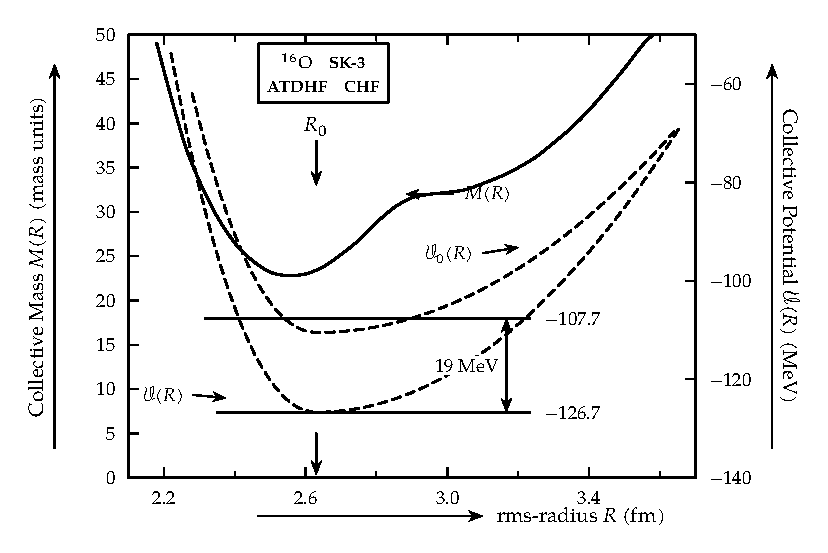
\includegraphics[width=0.75\textwidth]{pictures/12_6}
\par\end{centering}
\caption{\label{fig:12.6}ATDHF 理论中 $^{16}\mathrm{O}$ 同位旋标量单极模的势能面与质量参数。（引自
\cite{Go77}）}
\end{figure}

Giannoni 等人 \cite{GMQ76,GQ80} 计算了轻核同位旋标量四极模的质量参数。他们发现对于有效质量 $m^{*}/m\simeq1$
的 Skyrme 力，ATDHF 质量\ref{eq:12.110} 非常接近简单的 Cranking 质量 {[}见\ref{eq:12.147}{]}。事实上可以证明，\ref{eq:12.75a}
中产生 ATDHF 质量（Thouless-Valatin 质量）与 Cranking 质量（Inglis 公式）之差的项 $\Gamma_{1}$
正比于 $1-m^{*}/m$。

\subsection{绝热微扰论与Cranking公式\label{subsec:12.3.7}}

以微观方式导出集体运动惯性参数的最古老方法是所谓的 Cranking 公式。它最初由 Inglis \cite{In54,In56}
在转动情形下引入，我们在 5.4 节中对此进行了详细讨论。Kerman \cite{Ke61} 针对更一般的集体运动导出了类似的质量参数表达式。我们已在
12.3.2 节中看到，如果在动能\ref{eq:12.81} 中忽略自洽势 \ref{eq:12.74} 的时间奇宇称部分 $\Gamma_{1}$，我们将再次获得该公式。

该公式在过去被极为频繁地使用。因此，我们希望在此给出其在绝热微扰论背景下的通常推导 \cite{Wi55,In56,Be61a,Th61a}。为此，我们假设有一个单参数的
Hamilton 量族 $H(q)$，其中 $q$ 为集体坐标，例如描述核形状的形变参数。如果系统以确定的速度 $\dot{q}$
运动，它将由一个确定的时间函数 $q(t)$ 所表征。然而在实践中并不这样做，我们在推导集体 Hamilton 量时也不需要这种时间依赖关系的显式形式。我们仅仅假设运动是缓慢的。

在每个时刻 $t$，亦即对于每个形变 $q$，我们假设具有 Hamilton 量的本征态 $|k\rangle$，即所谓的绝热基底（adiabatic
basis）\cite{No77}：

\begin{equation}
H|k\rangle=E_{k}|k\rangle\label{eq:12.138}
\end{equation}

本征函数 $|k\rangle$ 以及能量都依赖于参数 $q$，从而依赖于时间 $t$。

Schrödinger 方程的精确解 $|\Psi(t)\rangle$：

\begin{equation}
H(t)|\Psi(t)\rangle=\mathrm{i}\hbar\frac{\partial}{\partial t}|\Psi(t)\rangle\label{eq:12.139}
\end{equation}

现在在该基底中展开：

\begin{equation}
|\Psi(t)\rangle=\sum_{k}a_{k}(t)\mathrm{e}^{\mathrm{i}\phi_{k}(t)}|k(t)\rangle\label{eq:12.140}
\end{equation}

为方便起见，我们在该展开中使用时间相关的相位因子：

\begin{equation}
\phi_{k}(t)=-\frac{1}{\hbar}\int^{t}E_{k}(t^{\prime})\,\mathrm{d}t^{\prime}\label{eq:12.141}
\end{equation}

这本质上处理了绝热态 $|k\rangle$ 的平凡振荡相位。将拟设\ref{eq:12.140} 代入 Schrödinger
方程 \ref{eq:12.139} 并左乘矢量 $\langle l|$，我们得到系数 $a_{k}$ 的一组耦合微分方程：

\begin{equation}
\dot{a}_{l}=-\sum_{k}\langle l|\frac{\partial}{\partial t}|k\rangle\mathrm{e}^{\mathrm{i}\phi_{kl}}a_{k}=-\dot{q}\sum_{k}\langle l|\frac{\partial}{\partial q}|k\rangle\mathrm{e}^{\mathrm{i}\phi_{kl}}a_{k}\label{eq:12.142}
\end{equation}

其中 $\phi_{kl}=\phi_{k}-\phi_{l}$。

该方程仍然是精确的。现在在绝热极限下，即对于小速度 $\dot{q}$ 研究它。我们假设系统在 $t=0$ 时处于绝热基态 $|0\rangle$（其中所有低于
Fermi 面的单粒子能级均被填满），初始条件为：

\begin{equation}
a_{k}(t=0)=\delta_{k0}\label{eq:12.143}
\end{equation}

由于 $a_{k}$ 的时间导数正比于 $\dot{q}$，我们预期在所有时刻，对于 $k\neq0$，$a_{k}(t)$
都很小，而 $a_{0}$ 接近于 1，即系统始终保持接近绝热基态。仅存在对更高态的虚激发，这些激发正比于速度并产生惯性。

在此近似下，对于 $l\neq0$ 我们得到：

\begin{equation}
\dot{a}_{l}=-\dot{q}\langle l|\frac{\partial}{\partial q}|0\rangle\mathrm{e}^{\mathrm{i}\phi_{0l}}\label{eq:12.144}
\end{equation}

在附加假设 $\dot{q}$ 和矩阵元 $\langle l|\partial/\partial q|0\rangle$ 与振荡相位
$\phi_{0l}$ 相比仅具有相对微弱的时间相关性下，我们可以对\ref{eq:12.144} 积分，对于 $l\neq0$
得到：

\begin{equation}
a_{l}=\frac{\mathrm{i}\hbar\dot{q}}{(E_{l}-E_{0})}\langle l|\frac{\partial}{\partial q}|0\rangle\mathrm{e}^{\mathrm{i}\phi_{0l}}\label{eq:12.145}
\end{equation}

由此，我们在有一阶微扰论中计算了波函数\ref{eq:12.140} 中依赖于速度的项，现在能够将总能量表示为“集体坐标” $q$
与相应速度 $\dot{q}$ 的函数：

\begin{equation}
E(q,\dot{q})=\langle\Psi(t)|H|\Psi(t)\rangle=E_{0}+\sum_{k\neq0}(E_{k}-E_{0})|a_{k}|^{2}=\frac{1}{2}M(q)\dot{q}^{2}+\mathcal{V}(q)\label{eq:12.146}
\end{equation}

其中势能为：

\begin{equation}
\mathcal{V}(q)=E_{0}(q)=\langle0|H|0\rangle_{q}\label{eq:12.146b}
\end{equation}

惯性参数即为著名的 Cranking 公式：

\begin{equation}
M(q)=2\hbar^{2}\sum_{k\neq0}\frac{|\langle k|\partial/\partial q|0\rangle|^{2}}{E_{k}-E_{0}}\label{eq:12.147}
\end{equation}

利用多体函数 $|k\rangle$ 为 Hamilton 量 $H(q)$ 的本征函数这一事实，我们可以将该公式略作改写：

\begin{equation}
M(q)=2\hbar^{2}\sum_{k\neq0}\frac{|\langle k|[H,\partial/\partial q]|0\rangle|^{2}}{(E_{k}-E_{0})^{3}}=2\hbar^{2}\sum_{k\neq0}\frac{|\langle k|\partial H/\partial q|0\rangle|^{2}}{(E_{k}-E_{0})^{3}}\label{eq:12.148}
\end{equation}

对于简化的 Nilsson Hamilton 量 $H=H_{0}-q\cdot Q$，我们从而得到：

\begin{equation}
M(q)=2\hbar^{2}\sum_{k\neq0}\frac{|\langle k|Q|0\rangle|^{2}}{(E_{k}-E_{0})^{3}}\label{eq:12.149}
\end{equation}

这一推导基于这样一个假设：绝热基底的状态不会随时间急剧变化。在单粒子能级在 Fermi 面处发生交叉的情形下，这一假设显然崩溃了。此时单粒子态从空态变为占有态，或者反之，且相应的两准粒子态的能量差
$E_{k}-E_{0}$ 趋于零。\ref{eq:12.147} 的分母趋于零，使得矩阵元 $\langle k|\partial/\partial q|0\rangle$
产生极大的峰值，从而 Cranking 公式的推导不再具有合理性。

事实上，当系统跨越这样一个交叉点运动时，可能会发生它不再保持在绝热基态中的情况。这在两个能级 $\epsilon_{1}$ 和 $\epsilon_{2}$
的孤立交叉点处最容易研究，设相互作用矩阵元为 $V_{12}$（两能级之间最接近的距离为 $2V_{12}$）。在此情形下，\ref{eq:12.142}
约化为两个耦合微分方程构成的系统。对于恒定速度 $\dot{q}$ 以及能级 $\epsilon_{1,2}$ 对 $q$ 的线性依赖，该问题可以解析求解。对于系统在赝交叉处跃迁到上层能级的几率
$P=|a_{2}(\infty)|^{2}$，我们得到 Landau-Zener 公式 \cite{La32,Ze32}：

\begin{equation}
P=\exp\left(-\frac{2\pi V^{2}_{12}}{\hbar|\dot{q}||(\mathrm{d}/\mathrm{d}q)(\epsilon_{1}-\epsilon_{2})|}\right)\label{eq:12.150}
\end{equation}

当速度增加时，该几率变大；同样地，当两能级斜率差增加时几率也变大，因为在这些情形下交换两能级性质的相互作用区域相当短暂。在该模型精确公式\ref{eq:12.150}
中，我们发现函数 $P$ 对小速度 $\dot{q}$ 表现出非解析行为 \cite{Sch77a}。通过将\ref{eq:12.142}
按 $\dot{q}$ 展开来求解（其最低阶给出了 Cranking 公式\ref{eq:12.147}），因此可能对应于一种渐近展开。

迄今为止，在何种情况下绝热近似崩溃在某种程度上仍是一个悬而未决的问题。如果使用严格的自洽计算（如 12.3.4 节所讨论的那样），该图景与在固定唯象势阱中的计算大不相同。由于在自洽场中对单粒子能级交叉的避免，绝热条件通常能够得到更好的满足。另一方面，在重离子反应中，速度通常很大，必须考虑越过能级交叉的跃迁。



\chapter{核物理中的半经典方法\label{chap:=006838=007269=007406=004E2D=007684=00534A=007ECF=005178=0065B9=006CD5}}

\section{引言\label{sec:13.1_=005F15=008A00}}

正如我们所见，用于处理原子核多体问题的诸多方法与形式理论是极为强大的，使我们能够解释海量的实验事实。然而在处理实际物理情形的具体数值计算中，贯彻如
Hartree-Fock、RPA 或时间相关 Hartree-Fock（TDHF）等微观形式理论往往需要付出极其庞大的计算工作量。因此，获得诸如原子核基态能量、密度以及巨共振频率等物理量的定性正确但简便快速的半经典估计，是非常切合实际需要的。

能够提供此类估计的方法在原子物理学中早已广为人知，在那里的自洽 Thomas-Fermi 理论给出了令人惊叹的优良结果 \cite{Go48}。而在理论核物理中，Thomas-Fermi
理论 \cite{SB63,Be71,MS69} 曾有很长一段时间未得到充分利用，因为正如我们将看到的，其原始形式极不适合直接处理包含极短程两体核力的多体系统。然而，近些年来
Thomas-Fermi 理论取得了若干重要进展 \cite{Ki67,BR71b,Gr72,BB72,BB74,BZ73,BJC76,BCK76,GS77,CJB77,DBS78}，使其在核物理中的广泛应用成为可能，这便是著名的扩展
Thomas-Fermi 理论（Extended Thomas-Fermi, ETF）。结果表明，相应的半经典表达式在“平均”意义上代表了各个物理量，即平滑掉了微观量子起伏。因此，它与
Strutinsky 平滑方法之间存在着深刻而紧密的类比。众所周知，若将 Strutinsky 平滑程序应用于现代 Hartree-Fock
计算 \cite{BQ75a,BQ75b}，其所对应的液滴能部分与唯象的 Bethe-Weizsäcker 质量公式吻合得极其出色。本章所阐述的半经典理论的核心宗旨，正在于针对平均物理量（密度等）建立一套自洽处理流程，使我们无需预先求解微观量子力学全解，即可直接计算出包含在
Hartree-Fock 计算中的宏观液滴能量部分。

一旦针对静态物理量建立起可靠的半经典方法，将其推广至动力学情形 \cite[及其中参考文献]{WMW75,HE78}
便是顺理成章的自然方向。在极限$\hbar\to0$下，TDHF 方程直接过渡为无碰撞 Boltzmann 方程。利用密度与势能半经典展开针对动力学情形的恰当推广，我们能够导出核流体动力学方程。核动力学系统作为一个
Fermi 体系，呈现出若干极其特异的性质，这些性质与经典普通流体的规律大相径庭；例如在零声（zero sound）激发中，甚至在很小的形变下局域动量分布也会发生显著的非球形畸变。

\section{静态情形\label{sec:13.2_=009759=006001=0060C5=005F62}}

\subsection{Thomas-Fermi 理论\label{subsec:13.2.1_Thomas-Fermi=007406=008BBA}}

Thomas-Fermi 理论 \cite{Th27,Fe28} 及其扩展，构成了核物理在独立粒子近似或 Hartree-Fock
近似框架下的半经典描述。因此，我们首先必须考察单粒子 Hamiltonian：

\[
H=-\frac{\hbar^{2}}{2m}\Delta+V,
\]

其中势场$V$原则上是自洽 Hartree-Fock 势 (5.34)。然而在随后的推导与演示中，我们通常假定核子仅仅是在给定的势阱（例如
Woods-Saxon 势）中独立运动。

在进一步推导之前，首先给出我们希望研究其半经典展开的各基本物理量的定义是有益的：

(i) 单粒子传播子（单粒子 Green 函数的虚时演化算符）：

\[
C^{t}(\boldsymbol{r},\boldsymbol{r}')=\langle\boldsymbol{r}|e^{-\mathrm{i}Ht/\hbar}|\boldsymbol{r}'\rangle,
\]

它是含时 Schrödinger 方程

\[
\mathrm{i}\hbar\frac{\partial}{\partial t}C^{t}(\boldsymbol{r},\boldsymbol{r}')=HC^{t}(\boldsymbol{r},\boldsymbol{r}'),
\]

在初始条件

\[
C^{t=0}(\boldsymbol{r},\boldsymbol{r}')=\delta(\boldsymbol{r}-\boldsymbol{r}')
\]

下的解。利用式 (13.1)，传播子亦可写为如下形式\footnote{原则上我们还应带有自旋指标$s,s'$。为简便起见，这里我们仅讨论自旋饱和系统（参见第 5.6.2 节），并通过统计因子 2 来考虑自旋。}：

\[
C^{\beta}(\boldsymbol{r},\boldsymbol{r}')=\sum_{i}\phi_{i}(\boldsymbol{r})\phi^{*}_{i}(\boldsymbol{r}')e^{-\beta\epsilon_{i}},
\]

为了行文方便，我们在此定义了参数$\beta=\mathrm{i}t/\hbar$。\footnote{选择符号$\beta$让人联想到倒温度，确实，若有$\beta=1/k_{B}T$（其中$k_{B}$为 Boltzmann
常数，$T$为温度），则式 (13.6) 将表示统计力学中的配分函数。然而，我们必须强调指出，在此处我们始终讨论的是$T=0$下的系统。}

(ii) 传播子的迹（配分函数；此处的因子 2 在后文中始终用于计及自旋简并）：

\[
Z(\beta)=\mathrm{Tr}\,C^{\beta}=2\int\mathrm{d}^{3}r\,C^{\beta}(\boldsymbol{r},\boldsymbol{r}).
\]

(iii) 谱密度矩阵：

\[
C^{\epsilon}(\boldsymbol{r},\boldsymbol{r}')=\langle\boldsymbol{r}|\delta(\epsilon-H)|\boldsymbol{r}'\rangle=\sum_{i}\phi_{i}(\boldsymbol{r})\phi^{*}_{i}(\boldsymbol{r}')\delta(\epsilon-\epsilon_{i}),
\]

利用它，传播子 (13.2) 可通过 Laplace 变换给出：

\[
C^{\beta}(\boldsymbol{r},\boldsymbol{r}')=\int^{\infty}_{0}\mathrm{d}\epsilon\,e^{-\beta\epsilon}C^{\epsilon}(\boldsymbol{r},\boldsymbol{r}'),
\]

在此我们假定了能量零点取在势阱底部。因此，谱密度矩阵由传播子的逆 Laplace 变换给出（关于 Laplace 变换的性质，参见
\cite{PB55,AS65}）：

\[
C^{\epsilon}(\boldsymbol{r},\boldsymbol{r}')=\frac{1}{2\pi\mathrm{i}}\int^{c+\mathrm{i}\infty}_{c-\mathrm{i}\infty}\mathrm{d}\beta\,e^{\beta\epsilon}C^{\beta}(\boldsymbol{r},\boldsymbol{r}')\quad(c>0).
\]

(iv) 能级态密度：

\[
g(\epsilon)=\mathrm{Tr}\,\delta(\epsilon-H)=\mathcal{L}^{-1}_{\beta\to\epsilon}Z(\beta).
\]

(v) 密度矩阵：

\[
\rho(\boldsymbol{r},\boldsymbol{r}';\lambda)=\sum^{\infty}_{\mu=1}\phi_{\mu}(\boldsymbol{r})\phi^{*}_{\mu}(\boldsymbol{r}')\Theta(\lambda-\epsilon_{\mu})=\frac{1}{2\pi\mathrm{i}}\int^{c+\mathrm{i}\infty}_{c-\mathrm{i}\infty}\frac{\mathrm{d}\beta}{\beta}e^{\beta\lambda}C^{\beta}(\boldsymbol{r},\boldsymbol{r}')\quad(c>0),
\]

其中$\Theta$为单位阶跃函数，$\lambda$为 Fermi 能量，此处我们利用了 Laplace 变换的一个基本性质（参见
\cite[第 29 章]{AS65}）。粒子数密度正是密度矩阵的局域对角部分（在随后的讨论中我们将看到，半经典近似的主要目的之一正是将核心物理量表达为该局域密度的泛函）：

\[
\rho(\boldsymbol{r})=\rho(\boldsymbol{r},\boldsymbol{r}).
\]

(vi) 动能密度 (5.85)：

\[
\tau(\boldsymbol{r})=\left.\boldsymbol{\nabla}_{\boldsymbol{r}}\cdot\boldsymbol{\nabla}_{\boldsymbol{r}'}\rho(\boldsymbol{r},\boldsymbol{r}';\lambda)\right|_{\boldsymbol{r}=\boldsymbol{r}'}=\sum^{A}_{i=1}|\boldsymbol{\nabla}\phi_{i}(\boldsymbol{r})|^{2}.
\]

(vii) 粒子数：

\[
N(\lambda)=\int\mathrm{d}^{3}r\,\rho(\boldsymbol{r};\lambda)=\int^{\lambda}_{-\infty}\mathrm{d}\epsilon\,g(\epsilon)=\mathcal{L}^{-1}_{\beta\to\lambda}\left[\frac{Z(\beta)}{\beta}\right].
\]

(viii) 基态能量：

\[
E(\lambda)=\int\mathrm{d}^{3}r\left.\left(-\frac{\hbar^{2}}{2m}\Delta+V(\boldsymbol{r})\right)\rho(\boldsymbol{r},\boldsymbol{r}';\lambda)\right|_{\boldsymbol{r}=\boldsymbol{r}'}=\int^{\lambda}_{-\infty}\mathrm{d}\epsilon\,\epsilon g(\epsilon)=\mathcal{L}^{-1}_{\beta\to\lambda}\left[\frac{Z(\beta)}{\beta^{2}}\right].
\]

在式 (13.15) 中，我们再次假定了核子处在给定的外势阱中；在自洽 Hartree-Fock 情形下，基态总能量需要作适当修正，如式
(5.40) 所示。

Thomas-Fermi 理论（例如参见 \cite{Th61b}）可以从截然不同的物理角度来阐释。在这里，我们采用相对通用的方式引入它，即假定空间各点处的粒子所感受到的势场局域地等于一个常数。我们将看到，这实际上也是一种短时间演化（或高温极限；参见第
529 页脚注）论证 \cite{Gr72}。为了切实推导出 Thomas-Fermi 近似，我们立即将研究置于一个更宽广的理论架构中，这将使我们随后能够极其自然地超越
Thomas-Fermi 近似。

为此，我们将式 (13.1) 中的势场$V(\boldsymbol{r})$在任意参考点$\boldsymbol{r}_{0}$附近展开为
Taylor 级数：

\[
V(\boldsymbol{r})=V(\boldsymbol{r}_{0})+\sum_{i}\left.\frac{\partial V}{\partial x_{i}}\right|_{\boldsymbol{r}=\boldsymbol{r}_{0}}(x_{i}-x_{0i})+\frac{1}{2}\sum_{ij}\left.\frac{\partial^{2}V}{\partial x_{i}\partial x_{j}}\right|_{\boldsymbol{r}=\boldsymbol{r}_{0}}(x_{i}-x_{0i})(x_{j}-x_{0j})+\dots
\]

如果该展开级数收敛，则利用式 (13.1) 和展开 (13.16) 求解式 (13.3) 所得到的传播子将精确独立于参考点$\boldsymbol{r}_{0}$的选择。若我们将展开
(13.16) 截断在第$n$阶，则相应的近似传播子$C^{(n)}_{\boldsymbol{r}_{0}}(\boldsymbol{r},\boldsymbol{r}')$将依赖于展开中心点$\boldsymbol{r}_{0}$，且相应的解仅在$\boldsymbol{r},\boldsymbol{r}'$充分靠近$\boldsymbol{r}_{0}$时才具有良好的精度。因此，最自然的最优选取是令极限$\boldsymbol{r},\boldsymbol{r}'\to\boldsymbol{r}_{0}$。由于参考点$\boldsymbol{r}_{0}$是任意的，我们将获得一个处处有效的局域传播子$C^{(n)}(\boldsymbol{r}_{0},\boldsymbol{r}_{0})$，即此时可将$\boldsymbol{r}_{0}$重新等同于空间原始坐标变量$\boldsymbol{r}$。然而这一步骤仅给出了传播子的局域对角部分；若我们希望保留传播子的非局域结构，最佳的处理方式不是让$\boldsymbol{r}$和$\boldsymbol{r}'$各自独立地趋于$\boldsymbol{r}_{0}$，而是假定我们在$\boldsymbol{r}$与$\boldsymbol{r}'$的质心坐标附近局域地展开势场；也就是说，我们将式
(13.3) 配合 (13.16) 的恰当解定义为 \cite{DBS78}：

\[
C^{(n)}(\boldsymbol{r},\boldsymbol{r}')=\lim_{\boldsymbol{r}_{0}\to\frac{1}{2}(\boldsymbol{r}+\boldsymbol{r}')}C^{(n)}_{\boldsymbol{r}_{0}}(\boldsymbol{r},\boldsymbol{r}').
\]

对于$n\to\infty$，若展开 (13.16) 收敛，则式 (13.17) 最终将渐近收敛于精确结果。对于有限的$n$，我们得到一系列逐级逼近的近似层次：$C^{(0)},C^{(1)},C^{(2)},\dots$，它们完全由势场及其前$n$阶导数表示。

正如本节开篇所述，Thomas-Fermi 近似的核心思想在于将势场在局域范围内视为常数。这显然对应于将级数展开 (13.16) 截断在最低阶（零阶）：

\[
\mathrm{i}\hbar\frac{\partial}{\partial t}C^{(0)}_{\boldsymbol{r}_{0}}=\left(-\frac{\hbar^{2}}{2m}\Delta+V(\boldsymbol{r}_{0})\right)C^{(0)}_{\boldsymbol{r}_{0}}.
\]

容易验证，方程 (13.18) 满足正确初始边界条件 (13.4) 的精确解析解为：

\[
C^{(0)}_{\boldsymbol{r}_{0}}(\boldsymbol{r},\boldsymbol{r}')=\left(\frac{m}{2\pi\hbar^{2}\beta}\right)^{3/2}e^{-\frac{m}{2\hbar^{2}\beta}(\boldsymbol{r}-\boldsymbol{r}')^{2}-\beta V(\boldsymbol{r}_{0})}.
\]

结合式 (13.19) 与 (13.11)，我们直接获得密度矩阵的 Thomas-Fermi 近似解析表达式 \cite[第 29 章]{AS65}：

\[
\rho^{\mathrm{TF}}(\boldsymbol{r},\boldsymbol{r}')=\frac{k^{3}_{F}(\boldsymbol{q})}{3\pi^{2}}\frac{3j_{1}(k_{F}(\boldsymbol{q})s)}{k_{F}(\boldsymbol{q})s}\Theta(\lambda-V(\boldsymbol{q})),
\]

其中相对坐标与中心质心坐标定义为：

\[
\boldsymbol{q}=\frac{1}{2}(\boldsymbol{r}+\boldsymbol{r}'),\quad\boldsymbol{s}=\boldsymbol{r}-\boldsymbol{r}',
\]

而$j_{1}$为一阶球 Bessel 函数。TF 密度矩阵的局域极限由此给出：

\[
\rho^{\mathrm{TF}}(\boldsymbol{r})=\frac{1}{3\pi^{2}}k^{3}_{F}(\boldsymbol{r})\Theta(\lambda-V(\boldsymbol{r})),
\]

式中局域 Fermi 动量定义为：

\[
k_{F}(\boldsymbol{r})=\left[\frac{2m}{\hbar^{2}}(\lambda-V(\boldsymbol{r}))\right]^{1/2}.
\]

必须强调的是，Fermi 能量$\lambda$由粒子数守恒归一化条件唯一确定：

\[
\int\mathrm{d}^{3}r\,\rho^{\mathrm{TF}}(\boldsymbol{r})=N,
\]

并且近似密度矩阵 (13.20) 已经失去了精确密度矩阵所固有的一些基本量子特征，例如幂等性$\rho^{2}=\rho$：

\[
\int\mathrm{d}^{3}r''\,\rho^{\mathrm{TF}}(\boldsymbol{r},\boldsymbol{r}'')\rho^{\mathrm{TF}}(\boldsymbol{r}'',\boldsymbol{r}')\neq\rho^{\mathrm{TF}}(\boldsymbol{r},\boldsymbol{r}'),
\]

其直接推论是（设$|\Phi\rangle$为 Slater 行列式，利用 Wick 定理但不满足$\rho^{2}=\rho$）：

\[
\langle\Phi|H|\Phi\rangle\neq\mathrm{Tr}(T\rho)+\frac{1}{2}\mathrm{Tr}_{1}\mathrm{Tr}_{2}(\rho\bar{v}\rho).
\]

因此，每当我们使用半经典密度进行变分计算时（见下文），我们必须像 BCS 理论（第 6 章）中那样，通过引入 Lagrange 乘子来附加粒子数归一化约束条件
(13.24)。

为了将 Thomas-Fermi 密度与精确微观量子密度进行直观对比，图 13.1 给出了 Woods-Saxon 势阱中两种密度的几何曲线分布。我们可以清楚地看到：在原子核内部，密度在“平均”意义上得到了极其优秀的再现；但在核表面弥散区，Thomas-Fermi
密度下降得过快，并在“经典转折点”处以零斜率截断降为零，经典转折点坐标由下式确定：

\[
\lambda-V(r_{\mathrm{cl}})=0.
\]

\begin{figure}[H]
\begin{centering}
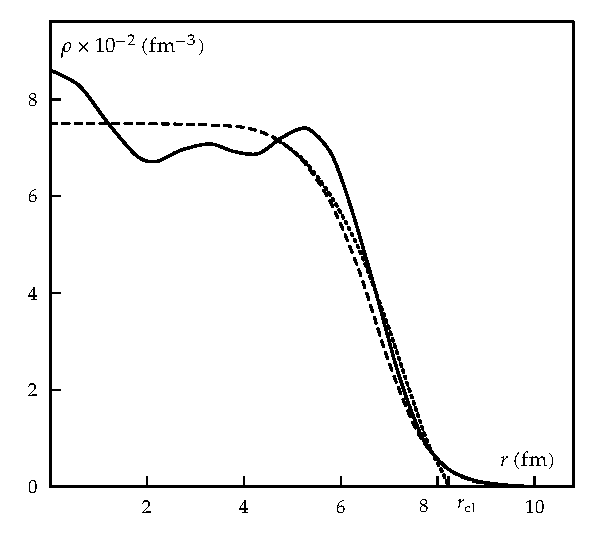
\includegraphics[width=0.75\textwidth]{pictures/13_1}
\par\end{centering}
\caption{\label{fig:13.1}图 13.1：在核子数$A=2N=184$的 Woods-Saxon 势阱中，精确密度（实线）与
Thomas-Fermi 近似（点线）的对比。势阱参数为：$V_{0}=-44\,\text{MeV}$，$a=0.67\,\text{fm}$，$R_{0}=1.27\,\text{fm}\cdot A^{1/3}$。虚线表示第
13.2.3 节的局域简谐近似（引自 \cite{DBS78}）。}
\end{figure}

总体而言，微观精确单粒子密度能够被式 (13.22) 这样简洁的形式描述到如此程度，是令人惊叹的。当我们利用式 (13.15) 结合
(13.19) 和 (13.6) 计算 Thomas-Fermi 近似下的基态总能量时，这一点表现得更加显著。采用与图 13.1 完全相同的势阱参数，数值积分计算结果为：

\[
E_{\mathrm{TF}}=-3194.5\,\text{MeV};\quad E_{\mathrm{exact}}=-3096.2\,\text{MeV}.
\]

在 Thomas-Fermi 近似下计算得到的重核结合能与精确微观值的相对偏差仅约为$\approx3\%$。这表明，在全空间积分的宏观大局物理量上，Thomas-Fermi
近似的精度甚至远高于单纯审视空间局域曲线（图 13.1）所能预期的水平。

比较式 (13.11) 与 (13.9)，可以直接得到如下微分恒等式：

\[
C^{\epsilon}(\boldsymbol{r},\boldsymbol{r}')=\partial_{\epsilon}\rho(\boldsymbol{r},\boldsymbol{r}';\epsilon),
\]

由此直接导出 Thomas-Fermi 近似下的能级态密度：

\[
g^{\mathrm{TF}}(\epsilon)=\frac{1}{2\pi^{2}}\left(\frac{2m}{\hbar^{2}}\right)^{3/2}\int\mathrm{d}^{3}r\,(\epsilon-V(\boldsymbol{r}))^{1/2}\Theta(\epsilon-V(\boldsymbol{r})).
\]

对于各向同性简谐振子势$V=\frac{1}{2}m\omega^{2}r^{2}$（我们在后文中将经常用它作为直观解析演示的标准范例），积分
(13.29) 可以完全解析积出，得到：

\[
g^{\mathrm{TF}}_{\mathrm{ho}}(\epsilon)=\frac{\epsilon^{2}}{2(\hbar\omega)^{3}}.
\]

在图 13.2 中，我们将该表达式对能量的积分（代表粒子数）与精确微观阶梯函数$N(\lambda)$进行了对比。我们再次看到，Thomas-Fermi
函数在宏观平均意义上极好地穿过了微观精确曲线\footnote{从$g^{\mathrm{TF}}(\epsilon)$在平均意义上代表精确态密度这一观察出发，我们无需使用极其繁复的“匹配连接条件”，即可立即直接导出通常的
WKB 量子化规则 \cite{Ar65}。关于 WKB 理论与 TF 理论如何系统联系的更详细内容，在此不作赘述 \cite{Vo77}。}；在后文中我们将对诸如$g(\epsilon)$等物理量的宏观“平均”如何严格数学定义给出更深入的讨论。

\begin{figure}[H]
\begin{centering}
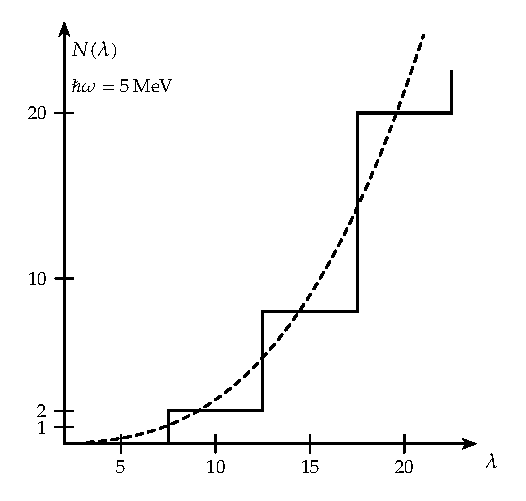
\includegraphics[width=0.65\textwidth]{pictures/13_2}
\par\end{centering}
\caption{\label{fig:13.2}图 13.2：简谐振子势中精确粒子数作为 Fermi 能的函数与相应 Thomas-Fermi 近似的对比。}
\end{figure}

为了计算 Thomas-Fermi 近似下的动能密度 (13.13)，我们结合式 (13.19) 和 (13.11)，得到：

\[
\tau^{\mathrm{TF}}(\boldsymbol{r})=\frac{1}{5\pi^{2}}\left(\frac{2m}{\hbar^{2}}\right)^{5/2}(\lambda-V(\boldsymbol{r}))^{5/2}\Theta(\lambda-V)=\frac{3}{5}\left(3\pi^{2}\right)^{2/3}\left(\rho^{\mathrm{TF}}\right)^{5/3}.
\]

在式 (13.31) 与 (13.22) 中消去$\lambda-V$，即建立起动能密度与局域密度之间的代数泛函关系（相应的式 (5.92)
计入了同位旋效应）：

\[
\tau^{\mathrm{TF}}=\frac{3}{5}(3\pi^{2})^{2/3}\rho^{5/3}.
\]

正如我们在引言中所指出的，由于两核子相互作用包含极强的短程性质，纯粹的 Thomas-Fermi 近似在核物理自洽场问题中几乎无能为力。这可以从以下事实清晰看出：对于
Skyrme 平均场势的局域部分$V[\rho]=a\rho+b\rho^{2}${[}参见式 (5.99){]}，非局域部分对它的修正极其微弱（这是核力短程性质的直接后果），式
(13.22) 关于密度$\rho$的解将导致空间各处完全均匀平庸的常数解，根本无法产生任何空间密度弥散分布。为了使半经典自洽理论在有限核中切实可行，我们必须对纯粹的
Thomas-Fermi 理论进行系统扩展，这将在随后的各小节中详尽讨论。

\subsection{Wigner-Kirkwood ℏ 展开\label{subsec:13.2.2_Wigner-Kirkwood=005C55=005F00}}

\subsubsection{形式体系\label{subsubsec:13.2.2.1_=005F62=005F0F=004F53=007CFB}}

我们现在希望展示，第 13.2.1 节中的 Thomas-Fermi 结果，实际上正是不同物理量（例如单粒子传播子 (13.2)）在按$\hbar$幂次作系统展开时的最低阶贡献。为此，转换至所谓的
Wigner 变换表象是极其方便的。单粒子算符$A$的 Wigner 变换定义为 \cite{Ar65}：

\[
A^{W}=A(\boldsymbol{q},\boldsymbol{p})=\int\mathrm{d}^{3}s\,e^{-\mathrm{i}\boldsymbol{p}\cdot\boldsymbol{s}/\hbar}\left\langle \boldsymbol{q}+\frac{1}{2}\boldsymbol{s}\right|A\left|\boldsymbol{q}-\frac{1}{2}\boldsymbol{s}\right\rangle ,
\]

其中$\boldsymbol{q}$与$\boldsymbol{s}$由式 (13.21) 给出。之所以采用 Wigner 表象极其便利，是因为在该表象中，例如
Hamiltonian (13.1) 恰好与其经典对应量严格一致：

\[
H^{W}(\boldsymbol{q},\boldsymbol{p})=\frac{\boldsymbol{p}^{2}}{2m}+V(\boldsymbol{q}).
\]

为了求出传播子 (13.2) 的完全经典部分，我们首先将其 Wigner 变换按$\beta$的幂次展开：

\[
C^{\beta}=e^{-\beta H}=\sum^{\infty}_{n=0}\frac{(-\beta)^{n}}{n!}H^{n}.
\]

这意味着我们必须求解单粒子算符乘积的 Wigner 变换。在附录 D 中，我们推导了如下乘积运算法则：

\[
(AB)^{W}=A(\boldsymbol{q},\boldsymbol{p})\exp\left[\frac{\mathrm{i}\hbar}{2}\left(\overleftarrow{\boldsymbol{\nabla}}_{\boldsymbol{q}}\cdot\overrightarrow{\boldsymbol{\nabla}}_{\boldsymbol{p}}-\overleftarrow{\boldsymbol{\nabla}}_{\boldsymbol{p}}\cdot\overrightarrow{\boldsymbol{\nabla}}_{\boldsymbol{q}}\right)\right]B(\boldsymbol{q},\boldsymbol{p}),
\]

其中箭头指示微分算符的作用方向：

\[
\Lambda=\frac{1}{2}\left(\overleftarrow{\boldsymbol{\nabla}}_{\boldsymbol{q}}\cdot\overrightarrow{\boldsymbol{\nabla}}_{\boldsymbol{p}}-\overleftarrow{\boldsymbol{\nabla}}_{\boldsymbol{p}}\cdot\overrightarrow{\boldsymbol{\nabla}}_{\boldsymbol{q}}\right).
\]

这一极其有用的式 (13.36) 使我们能够轻易验证诸如对易子的经典对应量正比于经典 Poisson 括号等著名结论 \cite{Go59}。利用式
(13.36)，我们亦可逐阶计算出展开 (13.35) 中出现的各阶项。例如计算至二阶项：

\[
(H^{2})^{W}=(H^{W})^{2}-\frac{\hbar^{2}}{4m}\Delta V.
\]

式 (13.38) 中的$\hbar$修正项源自动量算符与势能算符的非对易性。单粒子传播子 (13.2) 中正是源于动能部分与势能部分不对易而产生的这种$\hbar$依赖性，构成了我们所关注的焦点，也是我们旨在按$\hbar$的幂级数进行系统展开的对象；因此，在
Wigner 表象下我们无需担忧隐藏在$\beta$或其他表象转换过程中可能产生的其他微观依赖性。根据上述讨论显然可以看出，我们所讨论的$\hbar$展开借助展开式
(13.35) 与乘积法则 (13.36) 变得完全可行；$\hbar$的幂次在非经典修正项中始终为偶数，且精确等于特定项中关于空间与动量导数的阶数之和。因此，该展开在本质上同时也是一种梯度展开（gradient
expansion）。按$\hbar$的最低阶（零阶）表达式由 (13.35)、(13.36) 和 (13.38) 易于算出：

\[
C^{\beta}_{0}(\boldsymbol{q},\boldsymbol{p})=\exp\left[-\beta\left(\frac{p^{2}}{2m}+V(\boldsymbol{q})\right)\right].
\]

计算其逆 Wigner 变换，即对动量执行 Fourier 变换，恰好给出了我们之前在式 (13.19) 中得到的传播子局域 Thomas-Fermi
近似表达式。我们看到，Wigner 表象下的零阶项直接就是经典统计算符。由于式 (13.35) 是按$\hbar$与$\beta$的联立展开，对于高温（即极小的$\beta$），我们自然回归到经典统计物理结果。必须再次强调，在我们的核物理背景中，$\beta$绝不代表倒温度；相反，我们研究的是处于零温$T=0$的
Fermi 简并体系。另一方面，极其重要的一点在于：Thomas-Fermi 近似及其在随后的推导中所建立的扩展形式，严格遵循 Pauli
不相容原理。通过结合 (13.39) 与 (13.11) 从其 Wigner 变换直接计算密度，可以最为清晰地看出这一点：

\[
\rho^{\mathrm{TF}}(\boldsymbol{q})=\frac{2}{(2\pi\hbar)^{3}}\int\mathrm{d}^{3}p\,\mathcal{L}^{-1}_{\beta\to\lambda}\left[\frac{C^{\beta}_{0}(\boldsymbol{q},\boldsymbol{p})}{\beta}\right]=\frac{2}{(2\pi\hbar)^{3}}\int\mathrm{d}^{3}p\,\Theta\left(\lambda-\frac{p^{2}}{2m}-V(\boldsymbol{q})\right),
\]

\[
=\frac{1}{3\pi^{2}\hbar^{3}}[2m(\lambda-V(\boldsymbol{q}))]^{3/2}\Theta(\lambda-V(\boldsymbol{q})),
\]

这无非是对从零直至 Fermi 能级的所有有效量子动量$p\le[2m(\lambda-V)]^{1/2}$的相空间状态求和，且每个能级被自旋向上与向下的两个核子完全占据。

式 (13.35) 中$\beta$的幂次与$\hbar$的幂次并不是简单同步的，为了精确保留至$\hbar^{2}$阶，我们必须将式
(13.35) 展开至$\beta^{3}$阶。严格计算的结果为 \cite{Wi32,Wi34,Ki33,Ki57,JB75}：

\[
C^{\beta}(\boldsymbol{q},\boldsymbol{p})=\exp\left[-\beta\left(\frac{p^{2}}{2m}+V(\boldsymbol{q})\right)\right]\left\{ 1+\hbar^{2}\left[-\frac{\beta^{2}}{8m}\Delta V+\frac{\beta^{3}}{24m}(\boldsymbol{\nabla}V)^{2}+\frac{\beta^{3}}{24m^{2}}(\boldsymbol{p}\cdot\boldsymbol{\nabla})^{2}V\right]+\mathcal{O}(\hbar^{4})\right\} .
\]

表达式 (13.42) 使我们能够对第 13.2.1 节所考察的全部物理量获得系统的半经典量子修正。结合式 (13.11)，例如对于半经典密度矩阵的
Wigner 变换$f_{\mathrm{sc}}$（关于包含自旋-轨道耦合项的系统推广，参见 \cite{JBB75}），我们得到：

\[
f_{\mathrm{sc}}(\boldsymbol{q},\boldsymbol{p};\lambda)=\Theta\left(\lambda-\frac{p^{2}}{2m}-V(\boldsymbol{q})\right)+\hbar^{2}\left\{ -\frac{1}{8m}\Delta V\,\delta'\left(\lambda-\frac{p^{2}}{2m}-V\right)+\left[\frac{1}{24m}(\boldsymbol{\nabla}V)^{2}+\frac{1}{24m^{2}}(\boldsymbol{p}\cdot\boldsymbol{\nabla})^{2}V\right]\delta''\left(\lambda-\frac{p^{2}}{2m}-V\right)\right\} +\mathcal{O}(\hbar^{4}),
\]

式中半经典化学势$\lambda_{\mathrm{sc}}$由粒子数归一化约束 (13.14) 决定。在式 (13.43) 中，我们暂且忽略了正幂次$\beta$的逆
Laplace 变换在严格数学意义上不存在的问题。形式上通过将式 (13.11) 对$\lambda$进行微商来产生式 (13.42)
中不同幂次的$\beta$，我们在式 (13.43) 中获得了关于$\delta$函数的各阶导数。表达式 (13.43) 显然只能在广义函数（分布）的意义下加以理解与使用，但我们必须更深入地考察传播子的半经典展开
(13.42) 究竟在何种物理途径下才能发挥其强大威力。对动量$\boldsymbol{p}$积分式 (13.43)，我们直接获得包含二级梯度修正的半经典粒子数密度：

\[
\rho_{\mathrm{sc}}(\boldsymbol{r})=\frac{1}{3\pi^{2}}\left(\frac{2m}{\hbar^{2}}\right)^{3/2}(\lambda_{\mathrm{sc}}-V(\boldsymbol{r}))^{3/2}-\frac{1}{24\pi^{2}}\left(\frac{2m}{\hbar^{2}}\right)^{1/2}\left[\frac{\Delta V}{(\lambda_{\mathrm{sc}}-V)^{1/2}}+\frac{1}{4}\frac{(\boldsymbol{\nabla}V)^{2}}{(\lambda_{\mathrm{sc}}-V)^{3/2}}\right].
\]

这一半经典密度表达式不再包含任何阶跃$\delta$函数，然而在经典转折点$\lambda_{\mathrm{sc}}-V=0$处它发生病态发散，这使得我们必须重新审视此类展开的物理意义与适用范围。

\subsubsection{ℏ 展开的适用性与解释\label{subsubsec:13.2.2.2_=009002=007528=006027=004E0E=0089E3=0091CA}}

为了研究展开式 (13.42) 与 (13.43) 的有效性，考察若干能够严格解析求出传播子的理想势阱范例是极具启发性的：

(i) 对于一维线性势$V_{1}=ax$，容易验证如下传播子形式严格满足 Schrödinger 方程 (13.3)：

\[
C_{1}(x,x')=C^{(0)}_{1}(x,x')\exp\left[\frac{\hbar^{2}\beta^{3}}{24m}(V'_{1})^{2}\right],
\]

式中$V'_{1}$表示势场的一阶导数，而$C^{(0)}_{1}(x,x')$则是单粒子传播子 Thomas-Fermi 近似
(13.19) 的一维对应形式。式 (13.45) 的 Wigner 变换仅作用于$C^{(0)}_{1}$，剩余指数因子的半经典展开与式
(13.42) 括号中的表达式完全吻合；这可以轻而易举地加以验证。由此亦极其清楚地表明，对于此范例，展开 (13.42) 是完全严格成立的，并且在整个复$\beta$与$\hbar$平面上一致收敛。然而，在计算物理可观测量
{[}参见式 (13.7)–(13.15){]} 时，我们必须对形如 (13.42) 的展开执行逆 Laplace 变换，由此便产生了与式
(13.43) 相关联的数学困难。针对线性势范例 (13.45)，我们可以进行更详细的考察。利用式 (13.40) 以及 Laplace
变换的卷积定理 \cite{PB55,AS65}，线性势下的密度可以严格积出：

\[
f_{1}(q,p;\lambda)=2^{2/3}\sigma\int^{\infty}_{0}\mathrm{d}E\,\Theta\left(\lambda-\frac{p^{2}}{2m}-V_{1}(q)-E\right)\mathrm{Ai}\left(-2^{2/3}\sigma E\right),
\]

其中特征参数与 Airy 函数的积分表示分别为 \cite{AS65}：

\[
\sigma=\left(\frac{2m}{\hbar^{2}(V'_{1})^{2}}\right)^{1/3},\quad\mathrm{Ai}(z)=\frac{1}{2\pi}\int^{\infty}_{-\infty}\mathrm{d}s\,e^{\mathrm{i}(s^{3}/3+zs)}.
\]

在式 (13.47) 中作变量代换$y=2^{2/3}\sigma\beta$，我们看到当$\hbar\to0$时，$\mathrm{Ai}$渐近正比于$\delta(E)$，从而结合式
(13.46) 立即重新恢复出式 (13.43) 的首批主要项。通过将式 (13.45) 展开至$\hbar^{2}$，更高阶修正项亦可完全重现。由此我们可以洞察所有数学佯谬的根源：式
(13.46) 在本质上关于$\hbar$是非解析的，因此严格的常规$\hbar$幂级数展开在局域层面并不存在（这与函数$e^{-a/x}$在原点关于$x$的本性奇点完全类似）。

(ii) 作为第二个确定的解析范例，我们考察三维各向同性简谐振子势$V_{2}=\frac{1}{2}m\omega^{2}r^{2}$。容易验证，相应的含时
Schrödinger 方程 (13.3) 具有如下精确传播子解（详细推导可参见 \cite{Kr64}）：

\[
C_{2}(\boldsymbol{r},\boldsymbol{r}';\beta)=\left(\frac{m\omega}{2\pi\hbar\sinh(\beta\hbar\omega)}\right)^{3/2}\exp\left\{ -\frac{m\omega}{2\hbar\sinh(\beta\hbar\omega)}\left[(\boldsymbol{r}^{2}+\boldsymbol{r}'^{2})\cosh(\beta\hbar\omega)-2\boldsymbol{r}\cdot\boldsymbol{r}'\right]\right\} .
\]

在式 (13.15) 中我们需要该传播子的迹，容易算出其解析结果为：

\[
Z_{2}(\beta)=\mathrm{Tr}\,C^{\beta}_{2}=\frac{1}{4\sinh^{3}(\beta\hbar\omega/2)}.
\]

为了计算有效结合能项$E-\lambda N$，我们需要求出$\beta^{-2}Z(\beta)$的逆 Laplace 变换。对于式
(13.49) 的配分函数$Z_{2}$，这可以通过在复平面上沿虚轴左侧闭合围道积分来完成（取$\lambda>0$）。围道积分包含来自配分函数$Z_{2}$沿虚轴上每一个极点的留数贡献。原点$\beta=0$处的极点为五阶极点，而虚轴上的其他极点仅为三阶极点。为了计算原点处的留数，我们只需写出$Z_{2}(\beta)\beta^{-2}$直至$\beta^{-1}$阶的
Laurent 级数展开：

\[
\frac{Z_{2}(\beta)}{\beta^{2}}=\frac{2}{(\hbar\omega)^{3}}\frac{1}{\beta^{5}}\left[1-\frac{1}{8}(\beta\hbar\omega)^{2}+\frac{17}{1920}(\beta\hbar\omega)^{4}+\dots\right].
\]

计入原点极点以及虚轴上所有其余振荡极点的留数，我们获得能量的完整解析表达式：

\[
E-\lambda N=-\frac{\lambda^{4}}{12(\hbar\omega)^{3}}+\frac{\lambda^{2}}{8\hbar\omega}-\frac{17\hbar\omega}{960}+\dots+\text{（振荡项）}.
\]

从式 (13.51) 可以看出极其优美的物理图像：来自复原点$\beta=0$极点的贡献，作为$\lambda$的函数给出了一个单调平滑增长的部分；而远离实轴、沿虚轴分布的所有其余极点，则贡献出周期性剧烈振荡的项。这些振荡显然正是源于三维简谐势中高度简并的分立能级结构，而在单调线性势
(13.45) 中完全不存在这类虚轴极点。

尽管简谐振子势是非常特殊的解析范例，但我们完全可以将其核心物理结论推广至任意一般势阱：在式 (13.15) 中，函数$e^{\beta\lambda}Z(\beta)\beta^{-2}$在复原点处的奇点贡献直接给出了基态结合能的平滑宏观部分（液滴能），而分布在复平面其余位置的所有非零奇点贡献则直接构成了壳效应量子振荡项。

为了进一步证实这一点，我们考察第 2.9 节中研究的 Strutinsky 能级平滑方法与上述原点留数展开之间的严格数学联系。考察经曲率修正的高斯平滑态密度
(2.109)：

\[
\tilde{g}(\epsilon)=\frac{1}{\gamma}\int^{\infty}_{-\infty}\mathrm{d}\epsilon'\,g(\epsilon')f_{M}\left(\frac{\epsilon-\epsilon'}{\gamma}\right).
\]

利用配分函数的 Laplace 变换定义及卷积定理，对应于平滑态密度的平滑配分函数为：

\[
\tilde{Z}_{M}(\beta)=Z(\beta)\tilde{f}_{M}(\beta\gamma),
\]

其中平滑因子的 Laplace 变换为：

\[
\tilde{f}_{M}(\beta\gamma)=w(\beta\gamma)\sum^{M}_{m=0}\frac{(-1)^{m}}{2^{2m}m!}H_{2m}(0)(\beta\gamma)^{2m},
\]

\[
w(\beta\gamma)=e^{\beta^{2}\gamma^{2}/4}.
\]

在第 2.9 节中我们证明了，Strutinsky 平滑参数$\gamma$的取值必须在主壳间距$\hbar\omega$或更大的量级。这导致式
(13.54) 中的因子在振子配分函数 (13.49) 的第一个虚轴奇点处衰减了整整五个数量级以上！换言之，Strutinsky 平滑过程在物理本质上等价于在正负虚轴奇点之间截取一段配分函数，它尽可能长时间地保持等于精确配分函数，并在靠近壳层极点时以宽度$\gamma$迅速平滑降为零。因此，Strutinsky
平滑程序与我们上述将平滑能量定义为式 (13.15) 中来自$Z(\beta)$在原点处小$\beta$渐近行为的贡献是完全等价的
\cite{Je73,Je76}。

因此，式 (13.42) 所给出的半经典展开的巨大实用价值正在于：它直接提供了配分函数在原点附近关于$\hbar$与$\beta$的联立
Laurent 级数；这正是我们在计算来自原点奇点的结合能贡献时所需的全部物理信息。\footnote{应当指出，通过利用 Laurent 级数构建相应的 Padé 近似，原则上可以从$Z(\beta)$的半经典展开 (13.50)
重建其极点结构，从而将部分振荡壳效应重新包含进结合能中。然而，这一方向迄今尚未得到非常深入的系统研究 \cite{GS77}。}

\begin{table}[H]
\caption{\label{tab:13.1}表 13.1：与图 13.1 相同参数的球形 Woods-Saxon 势阱中的平滑结合能量（单位均为
MeV）。第一列为核子数$A=2N=2Z$。第二、三、四列分别给出$E_{\mathrm{TF}}$、$E^{(2)}_{\mathrm{sc}}$和$E^{(4)}_{\mathrm{sc}}$，分别对应式
(13.42) 中 TF 项、$\mathcal{O}(\hbar^{2})$项及$\mathcal{O}(\hbar^{4})$项的贡献。第五列给出总半经典能量$E_{\mathrm{sc}}$，最后一列给出
Strutinsky 平滑能量（引自 \cite{Je76}）。}

\centering{}<lyxtabular version=\textquotedbl 3\textquotedbl{} rows=\textquotedbl 4\textquotedbl{}
columns=\textquotedbl 6\textquotedbl ><features rotate=\textquotedbl 0\textquotedbl{}
tabularvalignment=\textquotedbl middle\textquotedbl ><column alignment=\textquotedbl center\textquotedbl{}
valignment=\textquotedbl top\textquotedbl ><column alignment=\textquotedbl center\textquotedbl{}
valignment=\textquotedbl top\textquotedbl ><column alignment=\textquotedbl center\textquotedbl{}
valignment=\textquotedbl top\textquotedbl ><column alignment=\textquotedbl center\textquotedbl{}
valignment=\textquotedbl top\textquotedbl ><column alignment=\textquotedbl center\textquotedbl{}
valignment=\textquotedbl top\textquotedbl ><column alignment=\textquotedbl center\textquotedbl{}
valignment=\textquotedbl top\textquotedbl ><row><cell alignment=\textquotedbl center\textquotedbl{}
valignment=\textquotedbl top\textquotedbl{} topline=\textquotedbl true\textquotedbl{}
bottomline=\textquotedbl true\textquotedbl{} leftline=\textquotedbl true\textquotedbl{}
usebox=\textquotedbl none\textquotedbl >$A$</cell><cell alignment=\textquotedbl center\textquotedbl{}
valignment=\textquotedbl top\textquotedbl{} topline=\textquotedbl true\textquotedbl{}
bottomline=\textquotedbl true\textquotedbl{} leftline=\textquotedbl true\textquotedbl{}
usebox=\textquotedbl none\textquotedbl >$E_{\mathrm{TF}}$</cell><cell
alignment=\textquotedbl center\textquotedbl{} valignment=\textquotedbl top\textquotedbl{}
topline=\textquotedbl true\textquotedbl{} bottomline=\textquotedbl true\textquotedbl{}
leftline=\textquotedbl true\textquotedbl{} usebox=\textquotedbl none\textquotedbl >$E^{(2)}_{\mathrm{sc}}$</cell><cell
alignment=\textquotedbl center\textquotedbl{} valignment=\textquotedbl top\textquotedbl{}
topline=\textquotedbl true\textquotedbl{} bottomline=\textquotedbl true\textquotedbl{}
leftline=\textquotedbl true\textquotedbl{} usebox=\textquotedbl none\textquotedbl >$E^{(4)}_{\mathrm{sc}}$</cell><cell
alignment=\textquotedbl center\textquotedbl{} valignment=\textquotedbl top\textquotedbl{}
topline=\textquotedbl true\textquotedbl{} bottomline=\textquotedbl true\textquotedbl{}
leftline=\textquotedbl true\textquotedbl{} usebox=\textquotedbl none\textquotedbl >$E_{\mathrm{sc}}$</cell><cell
alignment=\textquotedbl center\textquotedbl{} valignment=\textquotedbl top\textquotedbl{}
topline=\textquotedbl true\textquotedbl{} bottomline=\textquotedbl true\textquotedbl{}
leftline=\textquotedbl true\textquotedbl{} rightline=\textquotedbl true\textquotedbl{}
usebox=\textquotedbl none\textquotedbl >$E_{\mathrm{Str}}$</cell></row><row><cell
alignment=\textquotedbl center\textquotedbl{} valignment=\textquotedbl top\textquotedbl{}
topline=\textquotedbl true\textquotedbl{} leftline=\textquotedbl true\textquotedbl{}
usebox=\textquotedbl none\textquotedbl >164</cell><cell alignment=\textquotedbl center\textquotedbl{}
valignment=\textquotedbl top\textquotedbl{} topline=\textquotedbl true\textquotedbl{}
leftline=\textquotedbl true\textquotedbl{} usebox=\textquotedbl none\textquotedbl >-3344.7</cell><cell
alignment=\textquotedbl center\textquotedbl{} valignment=\textquotedbl top\textquotedbl{}
topline=\textquotedbl true\textquotedbl{} leftline=\textquotedbl true\textquotedbl{}
usebox=\textquotedbl none\textquotedbl >88.8</cell><cell alignment=\textquotedbl center\textquotedbl{}
valignment=\textquotedbl top\textquotedbl{} topline=\textquotedbl true\textquotedbl{}
leftline=\textquotedbl true\textquotedbl{} usebox=\textquotedbl none\textquotedbl >1.0</cell><cell
alignment=\textquotedbl center\textquotedbl{} valignment=\textquotedbl top\textquotedbl{}
topline=\textquotedbl true\textquotedbl{} leftline=\textquotedbl true\textquotedbl{}
usebox=\textquotedbl none\textquotedbl >-3254.9</cell><cell alignment=\textquotedbl center\textquotedbl{}
valignment=\textquotedbl top\textquotedbl{} topline=\textquotedbl true\textquotedbl{}
leftline=\textquotedbl true\textquotedbl{} rightline=\textquotedbl true\textquotedbl{}
usebox=\textquotedbl none\textquotedbl >-3256.0 (1.2)</cell></row><row><cell
alignment=\textquotedbl center\textquotedbl{} valignment=\textquotedbl top\textquotedbl{}
topline=\textquotedbl true\textquotedbl{} leftline=\textquotedbl true\textquotedbl{}
usebox=\textquotedbl none\textquotedbl >260</cell><cell alignment=\textquotedbl center\textquotedbl{}
valignment=\textquotedbl top\textquotedbl{} topline=\textquotedbl true\textquotedbl{}
leftline=\textquotedbl true\textquotedbl{} usebox=\textquotedbl none\textquotedbl >-5484.8</cell><cell
alignment=\textquotedbl center\textquotedbl{} valignment=\textquotedbl top\textquotedbl{}
topline=\textquotedbl true\textquotedbl{} leftline=\textquotedbl true\textquotedbl{}
usebox=\textquotedbl none\textquotedbl >119.7</cell><cell alignment=\textquotedbl center\textquotedbl{}
valignment=\textquotedbl top\textquotedbl{} topline=\textquotedbl true\textquotedbl{}
leftline=\textquotedbl true\textquotedbl{} usebox=\textquotedbl none\textquotedbl >1.1</cell><cell
alignment=\textquotedbl center\textquotedbl{} valignment=\textquotedbl top\textquotedbl{}
topline=\textquotedbl true\textquotedbl{} leftline=\textquotedbl true\textquotedbl{}
usebox=\textquotedbl none\textquotedbl >-5364.0</cell><cell alignment=\textquotedbl center\textquotedbl{}
valignment=\textquotedbl top\textquotedbl{} topline=\textquotedbl true\textquotedbl{}
leftline=\textquotedbl true\textquotedbl{} rightline=\textquotedbl true\textquotedbl{}
usebox=\textquotedbl none\textquotedbl >-5364.4 (0.8)</cell></row><row><cell
alignment=\textquotedbl center\textquotedbl{} valignment=\textquotedbl top\textquotedbl{}
topline=\textquotedbl true\textquotedbl{} bottomline=\textquotedbl true\textquotedbl{}
leftline=\textquotedbl true\textquotedbl{} usebox=\textquotedbl none\textquotedbl >416</cell><cell
alignment=\textquotedbl center\textquotedbl{} valignment=\textquotedbl top\textquotedbl{}
topline=\textquotedbl true\textquotedbl{} bottomline=\textquotedbl true\textquotedbl{}
leftline=\textquotedbl true\textquotedbl{} usebox=\textquotedbl none\textquotedbl >-9049.1</cell><cell
alignment=\textquotedbl center\textquotedbl{} valignment=\textquotedbl top\textquotedbl{}
topline=\textquotedbl true\textquotedbl{} bottomline=\textquotedbl true\textquotedbl{}
leftline=\textquotedbl true\textquotedbl{} usebox=\textquotedbl none\textquotedbl >162.5</cell><cell
alignment=\textquotedbl center\textquotedbl{} valignment=\textquotedbl top\textquotedbl{}
topline=\textquotedbl true\textquotedbl{} bottomline=\textquotedbl true\textquotedbl{}
leftline=\textquotedbl true\textquotedbl{} usebox=\textquotedbl none\textquotedbl >1.1</cell><cell
alignment=\textquotedbl center\textquotedbl{} valignment=\textquotedbl top\textquotedbl{}
topline=\textquotedbl true\textquotedbl{} bottomline=\textquotedbl true\textquotedbl{}
leftline=\textquotedbl true\textquotedbl{} usebox=\textquotedbl none\textquotedbl >-8881.5</cell><cell
alignment=\textquotedbl center\textquotedbl{} valignment=\textquotedbl top\textquotedbl{}
topline=\textquotedbl true\textquotedbl{} bottomline=\textquotedbl true\textquotedbl{}
leftline=\textquotedbl true\textquotedbl{} rightline=\textquotedbl true\textquotedbl{}
usebox=\textquotedbl none\textquotedbl >-8882.8 (1.2)</cell></row></lyxtabular>
\end{table}

在表 13.1 中，我们展示了球形 Woods-Saxon 势阱中基态能量平滑部分的逐阶收敛情况，并与精确的 Strutinsky
平滑值进行了严格比对。极为引人注目的是：包含至$\hbar^{4}$阶展开即可获得高度精确收敛的宏观数值，且与 Strutinsky
能量在极高精度下完美吻合。来自复原点极点的半经典能量几乎穷尽了体系基态总能量的绝大部分（微观壳效应仅占千分之几的量级）。然而，这千分之几的细微能量起伏包含了原子核形变势能面上诸如双裂变势垒等极具决定性的微观结构效应。

\subsubsection{动能密度泛函\label{subsubsec:13.2.2.3_=0052A8=0080FD=005BC6=005EA6=006CDB=0051FD}}

克服无法直接开展自洽半经典迭代计算困难的一个极具吸引力的突破口如下\footnote{在本节的讨论中，我们在很大程度上参考了 \cite{Bs77} 中给出的阐述。}：在计算基态能量时，我们需要式
(13.13) 所定义的动能密度$\tau(\boldsymbol{r})$。如果我们能够将动能密度完全表达为局域密度$\rho(\boldsymbol{r})$的泛函，即$\tau=\tau[\rho(\boldsymbol{r})]$，那么由于诸如
Skyrme 势能密度 (5.87) 本身完全由$\rho$和$\tau$构成，原子核总结合能将成为局域密度$\rho(\boldsymbol{r})$的纯粹单变量泛函。随后只需对$\rho$进行能量变分，即可直接导出关于局域密度$\rho(\boldsymbol{r})$的闭合微分方程。尽管
Hohenberg-Kohn 定理 \cite{HK64,MT77} 已经从理论上严格确立了任意多 Fermion 体系的基态能量及动能密度都是局域密度的唯一泛函，但在实际微观计算中推导这一泛函的精确解析形式是极端困难的。而在我们的半经典理论体系中，我们却能够系统构造出完全自洽的渐近泛函形式：

\[
\tau_{\mathrm{sc}}(\boldsymbol{r},\lambda)=\frac{3}{5}\left(\frac{2m}{\hbar^{2}}\right)^{5/2}\frac{1}{3\pi^{2}}(\lambda-V)^{5/2}-\frac{\hbar^{2}}{8m}\frac{1}{3\pi^{2}}\left(\frac{2m}{\hbar^{2}}\right)^{3/2}\left[5\Delta V(\lambda-V)^{1/2}-\frac{9}{4}\frac{(\boldsymbol{\nabla}V)^{2}}{(\lambda-V)^{1/2}}\right]+\mathcal{O}(\hbar^{4}).
\]

将密度表达式 (13.44) 及其梯度展开结合，消去势场导数，最终导出了著名的动能密度泛函 \cite{Ki67,Je76}\footnote{有时为了更精确地重现表面能，人们会采用略微不同于$1/36$的唯象唯理加权系数 \cite{Ba72b}。}：

\[
\tau[\rho]=\frac{3}{5}(3\pi^{2})^{2/3}\rho^{5/3}+\frac{1}{36}\frac{(\boldsymbol{\nabla}\rho)^{2}}{\rho}+\frac{1}{3}\Delta\rho.
\]

式 (13.57) 右端第一项正是无限均匀核物质的 Thomas-Fermi 主导项；第二项被称为 Weizsäcker 梯度修正项；而最后一项为空间全散度项，由
Gauss 定理可知它对全空间动能积分不产生净贡献。

\begin{figure}[H]
\begin{centering}
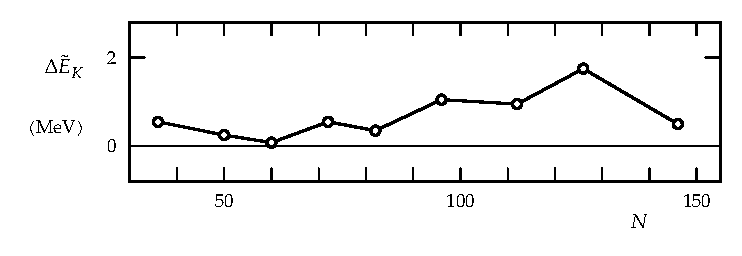
\includegraphics[width=0.65\textwidth]{pictures/13_3}
\par\end{centering}
\caption{\label{fig:13.3}图 13.3：动能差值$\Delta\tilde{E}_{K}=\tilde{E}_{K}-\tilde{T}_{K}$，其中$\tilde{E}_{K}$为
Strutinsky 平滑动能，$\tilde{T}_{K}$按文中动能泛函计算。数值为球形 Woods-Saxon 势阱中作为中子数$N$的函数（引自
\cite{BJC76}）。}
\end{figure}


\subsubsection{变分计算\label{subsubsec:13.2.2.4_=0053D8=005206=008BA1=007B97}}

获得泛函 (13.57) 后，我们即可通过变分原理自洽确定半经典密度分布\footnote{此处的变分原理在与一般能量泛函$E[\rho]$相联系时，并不严格等同于第 5.6.1.2 节中基于多体态矢的 Ritz 严格上界变分。}：

\[
\delta\left(E[\rho]-\lambda\int\mathrm{d}^{3}r\,\rho(\boldsymbol{r})\right)=0.
\]

为展示核心物理图像，忽略有效质量与自旋-轨道耦合项，取能量密度泛函为：

\[
E[\rho]=\int\mathrm{d}^{3}r\,\mathcal{E}[\rho],\quad\mathcal{E}[\rho]=\mathcal{E}_{\infty}(\rho)+\frac{\hbar^{2}}{2m}\frac{1}{36}\frac{(\boldsymbol{\nabla}\rho)^{2}}{\rho},
\]

在核物质饱和密度$\rho_{0}\approx0.14\,\text{fm}^{-3}$附近将其参数化展开为不可压缩模量$K$的形式：

\[
\mathcal{E}_{\infty}(\rho)\simeq\mathcal{E}_{0}+\frac{K}{18}\left(\frac{\rho-\rho_{0}}{\rho_{0}}\right)^{2}.
\]

变分方程直接导出密度的二阶非线性常微分方程：

\[
\Delta\rho-\frac{1}{2}\frac{(\boldsymbol{\nabla}\rho)^{2}}{\rho}-\frac{18m}{\hbar^{2}}\rho\frac{\partial\mathcal{E}_{\infty}}{\partial\rho}+\frac{18m}{\hbar^{2}}\lambda\rho=0.
\]

在核表面渐近区，式 (13.62) 简化为 Berg-Wilets 方程 \cite{BW56}：

\[
\Delta\sqrt{\rho}-\frac{1}{a^{2}}\sqrt{\rho}=0,
\]

其球对称渐近解具有指数衰减形式：

\[
\rho(r)\sim\frac{1}{r^{2}}e^{-2r/a}.
\]

\begin{figure}[H]
\begin{centering}
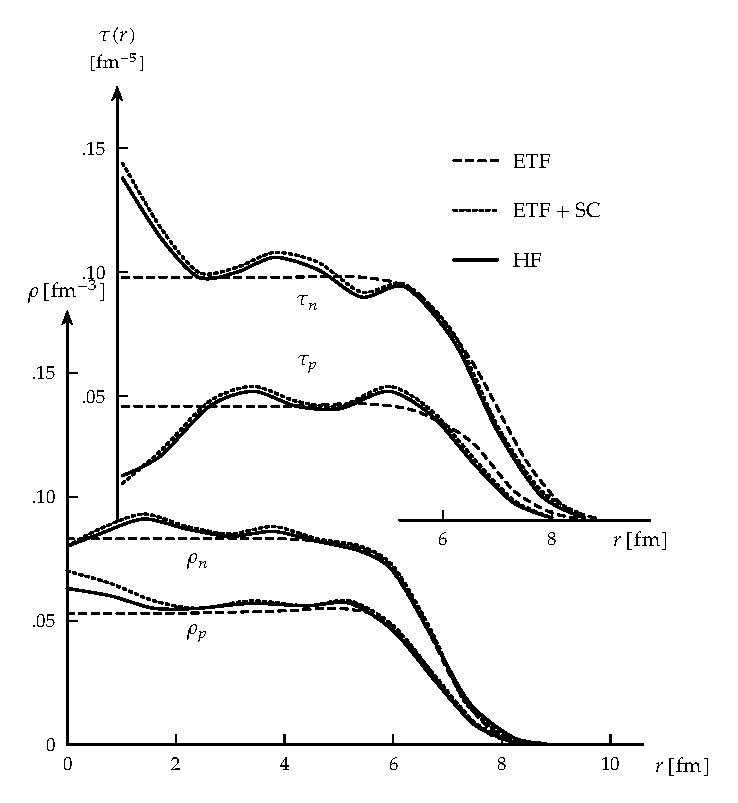
\includegraphics[width=0.75\textwidth]{pictures/13_4}
\par\end{centering}
\caption{\label{fig:13.4}图 13.4：自洽半经典密度与动能密度剖面与 Skyrme Hartree-Fock 微观精确结果的对比
\cite{BCK76}。}
\end{figure}


\subsection{ℏ 展开的部分求和\label{subsec:13.2.3_=0090E8=005206=006C42=00548C}}

上一小节表明，虽然扩展 Thomas-Fermi 能够极好地给出能量的平滑部分，但在经典转折点附近其密度仍显现出过陡的下降行为。为了解决这一局限，我们重新审视展开
(13.16)。如果在一维情形下保留一阶导数（线性化势场），传播子严格解析可求 \cite{Sw55,Gr72,DBS78}：

\[
C^{(1)}(q,s)=\left(\frac{m}{2\pi\hbar^{2}\beta}\right)^{1/2}\exp\left[-\frac{m}{2\hbar^{2}\beta}s^{2}-\beta V(q)+\frac{\hbar^{2}\beta^{3}}{24m}\left(\frac{\partial V}{\partial q}\right)^{2}\right].
\]

进一步在展开 (13.16) 中保留至势场的二阶导数项，即构建所谓的局域简谐近似（locally harmonic approximation）。借助简谐振子解
(13.48) 作为指导，一维局域简谐传播子的严格解析表达式为 \cite{Gr72,DBS78}：

\[
C^{(2)}(q,s)=\left(\frac{m\omega(q)}{2\pi\hbar\sinh(\beta\hbar\omega(q))}\right)^{1/2}\exp\left\{ -\frac{m\omega(q)}{4\hbar}\left[\tanh\left(\frac{\beta\hbar\omega(q)}{2}\right)s^{2}+4\frac{(q-\bar{q})^{2}}{\tanh\left(\frac{\beta\hbar\omega(q)}{2}\right)}\right]-\beta\bar{V}(q)\right\} ,
\]

其中特征参数定义为：$\omega(q)=[V''(q)/m]^{1/2}$，$\bar{q}(q)=q-V'(q)/V''(q)$，以及$\bar{V}(q)=V(q)-[V'(q)]^{2}/[2V''(q)]$。这一部分求和方案极其出色地再现了波函数向经典禁区穿透的量子隧道效应。

\begin{figure}[H]
\begin{centering}
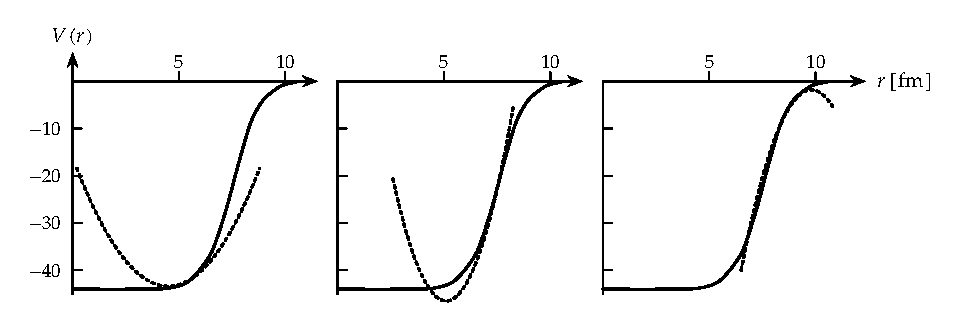
\includegraphics[width=0.65\textwidth]{pictures/13_5}
\par\end{centering}
\caption{\label{fig:13.5}图 13.5：在一维 Woods-Saxon 势阱中三个不同坐标点处的局域抛物线近似。}
\end{figure}


\subsection{鞍点法\label{subsec:13.2.4_=00978D=0070B9=006CD5}}

为了从局域简谐传播子中解析抽取平滑态密度与能量，可以高效借助复平面鞍点法（Saddle Point Method, SPM）\cite{PB75,Bh77}。将逆
Laplace 积分写为$G(\lambda)=\frac{1}{2\pi\mathrm{i}}\int^{c+\mathrm{i}\infty}_{c-\mathrm{i}\infty}\mathrm{d}\beta\,e^{S(\beta)}$，并将指数项$S$在实轴驻点$\beta_{0}$处展开，系统考虑高阶涨落修正。

\begin{figure}[H]
\begin{centering}
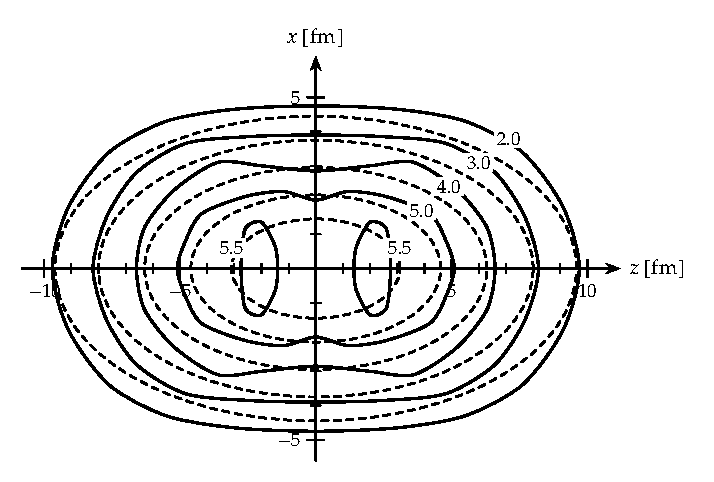
\includegraphics[width=0.75\textwidth]{pictures/13_6}
\par\end{centering}
\caption{\label{fig:13.6}图 13.6：强形变简谐振子势中，微观精确密度与采用鞍点法获得的平滑半经典密度的对比（感谢 J.
Bartel 提供此图）。}
\end{figure}


\subsection{球形 Woods-Saxon 势的应用\label{subsec:13.2.5_Woods-Saxon=005E94=007528}}

结合局域简谐传播子 (13.66) 与鞍点法，构成了本理论的核心基础。在图 13.1 中，采用局域简谐近似获得的密度（虚线）在核表面弥散尾区与精确微观结果展现出令人信服的极佳吻合，彻底克服了原
ETF 密度泛函在表面过渡过陡的理论缺陷。平均单粒子能量和与 Strutinsky 宏观平滑值在全质量区内的偏差仅在 5–10 MeV
范围以内。

\subsection{对性质的半经典处理\label{subsec:13.2.6_=005BF9=006027=008D28=005904=007406}}

在建立起自洽单粒子密度的半经典描述后，将其推广至包含配对关联的 BCS 理论框架是非常自然的（参见第 6、7 章）。在极限$\hbar\to0$下，广义准粒子密度对易子方程退化为经典
Poisson 括号，由此直接导出半经典能隙方程（gap equation）：

\[
\Delta(\boldsymbol{q},\boldsymbol{p})=-\frac{1}{2}\int\frac{\mathrm{d}^{3}k}{(2\pi\hbar)^{3}}v(\boldsymbol{p}-\boldsymbol{k})\frac{\Delta(\boldsymbol{q},\boldsymbol{k})}{\sqrt{h^{2}(\boldsymbol{q},\boldsymbol{k})+\Delta^{2}(\boldsymbol{q},\boldsymbol{k})}}.
\]

\begin{figure}[H]
\begin{centering}
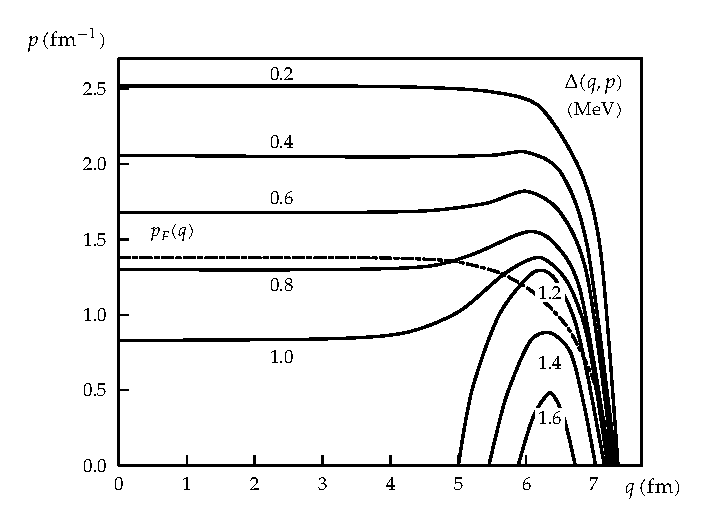
\includegraphics[width=0.7\textwidth]{pictures/13_7}
\par\end{centering}
\caption{\label{fig:13.7}图 13.7：Wigner 相空间中的中子配对能隙分布$\Delta(q,p)$，采用参数为$V_{0}=-49\,\text{MeV}$、$R_{0}=6.81\,\text{fm}$、$a=0.66\,\text{fm}$的
Woods-Saxon 势阱，中子数$N=96$。两体配对相互作用参数为$V_{0}=-28\,\text{MeV}$，$r_{0}=1.6\,\text{fm}$。}
\end{figure}

\begin{figure}[H]
\begin{centering}
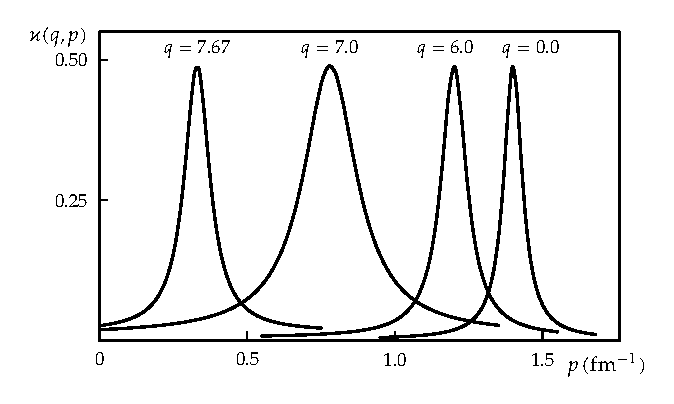
\includegraphics[width=0.65\textwidth]{pictures/13_8}
\par\end{centering}
\caption{\label{fig:13.8}图 13.8：原子核中不同空间位置$q$处的配对张量$\kappa(q,p)$（参数与图 13.7
相同）。}
\end{figure}

\begin{figure}[H]
\begin{centering}
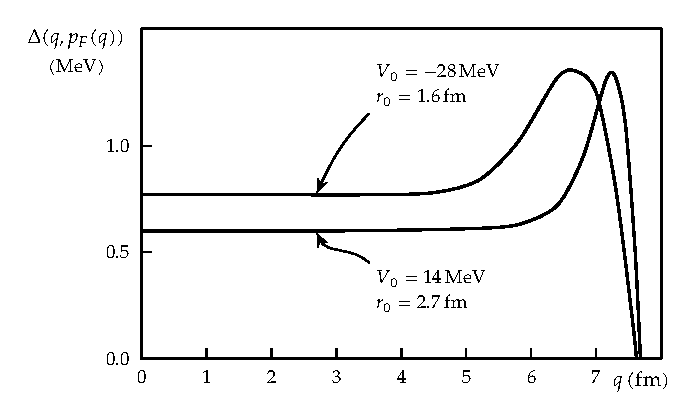
\includegraphics[width=0.65\textwidth]{pictures/13_9}
\par\end{centering}
\caption{\label{fig:13.9}图 13.9：沿局域 Fermi 面 {[}$p_{F}(q)${]} 的配对能隙分布曲线，展示了两组给出相同宏观配对能的不同核力参数的计算结果。}
\end{figure}

从图 13.7–13.9 可以清晰看出，理论计算揭示出配对能隙高度集中分布在原子核表面弥散区，表明核物理中的配对现象在本质上是一种强烈的表面效应，这对理解双核子转移反应等前沿实验过程具有至关重要的指导意义。

\section{动态情形\label{sec:13.3_=0052A8=006001=0060C5=005F62}}

至此，我们已经运用半经典方法系统研究了原子核的静态物理性质，例如核密度分布与原子核结合能。极其自然的研究延伸是将这些理论进一步推广至动力学过程，例如
RPA 与时间相关 Hartree-Fock（TDHF）理论。为此，我们必须探寻这些微观量子多体动力学理论在$\hbar\to0$时的经典极限。在动力学情形下，涌现出一系列全新的物理特征与理论课题，目前物理学界尚处于深入探索的初级阶段；因此，在这一最后章节中，我们不可能做到面面俱到，而是着重勾勒该理论的核心脉络与物理图像。

动力学情形下的基石性方程之一，乃是时间相关 Hartree-Fock 方程 (12.9) 的经典极限，它将直接引申出原子核流体动力学方程。另一条稍有不同的推导路径则是基于含时变分原理建立此类方程。此外，我们还将揭示局域动量分布在动态情形下的非球形畸变现象，并讨论半经典结论与第
8 章能量加权和规则之间的深刻内在对应。

\subsection{Boltzmann 方程\label{subsec:13.3.1_Boltzmann=0065B9=007A0B}}

为了求取 TDHF 方程 (12.9) 的经典极限，我们必须取其 Wigner 变换，这可以借助附录 D 中的算符乘积运算法则 (D.55)
来实现。由此导出的微观严格方程为 \cite{Gr46,KK76}：

\[
\frac{\partial f(\boldsymbol{q},\boldsymbol{p},t)}{\partial t}=\frac{2}{\hbar}\sin\left[\frac{\hbar}{2}\left(\boldsymbol{\nabla}^{H}_{\boldsymbol{q}}\cdot\boldsymbol{\nabla}^{f}_{\boldsymbol{p}}-\boldsymbol{\nabla}^{H}_{\boldsymbol{p}}\cdot\boldsymbol{\nabla}^{f}_{\boldsymbol{q}}\right)\right]H(\boldsymbol{q},\boldsymbol{p})f(\boldsymbol{q},\boldsymbol{p},t),
\]

式中$f(\boldsymbol{q},\boldsymbol{p},t)$是密度矩阵$\rho$的 Wigner 变换 {[}参见式
(13.41){]}，而$H(\boldsymbol{q},\boldsymbol{p})$是单体 Hartree-Fock Hamiltonian
的 Wigner 变换。为简便起见，我们暂且假定外势场是局域的，但利用式 (13.36) 很容易推广至诸如 Skyrme 型非局域势。从式
(13.68) 令$\hbar\to0$，我们极其直接地获得其经典极限：

\[
\frac{\partial f^{(0)}}{\partial t}+\frac{\boldsymbol{p}}{m}\cdot\boldsymbol{\nabla}_{\boldsymbol{q}}f^{(0)}-\boldsymbol{\nabla}_{\boldsymbol{q}}V\cdot\boldsymbol{\nabla}_{\boldsymbol{p}}f^{(0)}=0.
\]

该方程在经典统计力学中最广为人知的名称便是无碰撞 Boltzmann 方程（collisionless Boltzmann equation）\cite{UF74,Hu63}，而$(2\pi\hbar)^{-3}f^{(0)}(\boldsymbol{q},\boldsymbol{p},t)$则是相应的经典相空间分布函数。式
(13.69) 的物理内涵极其清晰直观，它无非表述了经典相空间微元内粒子流入与流出的精确平衡：第一项是分布函数的局域显含时演化率；第二项描述由于微元内粒子具有有限运动速度而引起的漂移变化；第三项则代表由于平均场力导致的粒子动量加速度改变。因此，无碰撞
Boltzmann 方程在本质上宣告了随体相空间微元内的粒子数全时间微商恒等于零：$\mathrm{d}f^{(0)}/\mathrm{d}t=0$。

这显然仅适用于独立核子在平均场势垒边缘发生弹性反射、而体系内部不存在微观真正两体直接碰撞的情形。这一无碰撞特征正深深根植于我们作为出发点的
TDHF 平均场理论。若考虑真实核子-核子微观碰撞，则分布函数方程右侧必须引入两体碰撞积分项：$\mathrm{d}f^{(0)}/\mathrm{d}t=I(f^{(0)})$，该碰撞项亦可在$\hbar\to0$极限下由我们在导出
TDHF 时所略去的两体关联函数 (12.6) 系统还原 \cite{KB62,Sch72a}。在低激发能的原子核集体运动中，由于核子在基态原子核内的平均自由程与核几何线度相当（第
4 章），在初级近似下忽略两体碰撞项是完全合理且高度成立的 \cite{KK68}。

由方程 (13.69) 出发，建立 RPA 方程的经典对应物是极其平易的，因为正如第 8.5 节所示，RPA 在本质上正是 TDHF
方程的线性化小振幅展开。取最简单的局域势拟设$V[\rho]=a\rho(\boldsymbol{q})+b\rho^{2}(\boldsymbol{q})${[}参见式
(5.99){]}，在线性化微扰下引入展开：

\[
f(\boldsymbol{q},\boldsymbol{p},t)=f^{(0)}(\boldsymbol{q},\boldsymbol{p})+\delta f(\boldsymbol{q},\boldsymbol{p},t),\quad\rho(\boldsymbol{q},t)=\rho^{(0)}(\boldsymbol{q})+\delta\rho(\boldsymbol{q},t),
\]

\[
\delta\rho(\boldsymbol{q},t)=\frac{2}{(2\pi\hbar)^{3}}\int\mathrm{d}^{3}p\,\delta f(\boldsymbol{q},\boldsymbol{p},t),\tag{13.70b}
\]

由此导出的线性化方程为：

\[
\frac{\partial\delta f}{\partial t}+\frac{\boldsymbol{p}}{m}\cdot\boldsymbol{\nabla}_{\boldsymbol{q}}\delta f-\boldsymbol{\nabla}_{\boldsymbol{q}}V^{(0)}\cdot\boldsymbol{\nabla}_{\boldsymbol{p}}\delta f-\boldsymbol{\nabla}_{\boldsymbol{p}}f^{(0)}\cdot\boldsymbol{\nabla}_{\boldsymbol{q}}\left[(a+2b\rho^{(0)})\delta\rho\right]=0.
\]

在均匀无限核物质中，式 (13.71) 的第三项严格为零，方程存在精确的解析解 \cite{KB62,No64a}。解析解显示，微扰$\delta f$在球对称平衡动量球上叠加了一个非各向同性的、呈椭球/卵形畸变且绕平衡球作四极振荡的附加分布。这种特殊的量子统计振荡模式被称为零声（zero
sound），它与经典普通流体中的流体力学第一声（普通声波，其中 Fermi 球仅作各向同性的平移与胀缩振动）具有截然不同的微观物理本质。

\subsection{由 Boltzmann 方程导出流体动力学方程\label{subsec:13.3.2_=006D41=004F53=0052A8=00529B=005B66=005BFC=0051FA}}

为了降低求解方程 (13.69) 与 (13.71) 的庞大复杂度，人们通常通过将方程乘以动量$\boldsymbol{p}$的不同幂次并对动量执行积分，将其转换为关于$f(\boldsymbol{q},\boldsymbol{p},t)$的各阶动量矩的耦合微分方程组。将方程
(13.69) 对动量分别作零阶矩、一阶矩及二阶矩积分，经过系统的代数整理，最终化为五条著名的守恒律方程：

\[
\frac{\partial\rho}{\partial t}+\sum_{i}\frac{\partial}{\partial q_{i}}(\rho u_{i})=0,
\]

\[
\rho\left(\frac{\partial u_{i}}{\partial t}+\sum_{j}u_{j}\frac{\partial u_{i}}{\partial q_{j}}\right)=-\frac{\rho}{m}\frac{\partial V}{\partial q_{i}}-\frac{1}{m}\sum_{j}\frac{\partial P_{ij}}{\partial q_{j}},
\]

\[
\frac{\partial Q}{\partial t}+\sum_{i}\frac{\partial}{\partial q_{i}}(Qu_{i})+\sum_{ij}P_{ij}D_{ij}+\sum_{i}\frac{\partial W_{i}}{\partial q_{i}}=0.
\]

在此我们引入了流体动力学中标准的核心物理量定义：

局域平均流速：$u_{i}(\boldsymbol{q},t)=\overline{p_{i}/m}$；相对平均流速的热运动速度涨落：$U_{i}(\boldsymbol{q},\boldsymbol{p},t)=p_{i}/m-u_{i}$；热动能密度：$Q(\boldsymbol{q},t)=\frac{1}{2}m\rho\overline{\boldsymbol{U}^{2}}$；压力张量（动量流密度）：$P_{ij}(\boldsymbol{q},t)=m\rho\overline{U_{i}U_{j}}$；热流密度矢量：$W_{i}(\boldsymbol{q},t)=\frac{1}{2}m\rho\overline{U_{i}\boldsymbol{U}^{2}}$；应变率张量：$D_{ij}(\boldsymbol{q},t)=\frac{1}{2}\left(\frac{\partial u_{i}}{\partial q_{j}}+\frac{\partial u_{j}}{\partial q_{i}}\right)$。

方程 (13.72)–(13.74) 严格表达了质量连续性守恒、动量平衡以及内能流平衡。然而，这组方程本身并不是闭合的，因为压力张量和热流矢量包含更高阶的动量矩未决函数。在普通流体力学与低能核多体物理中，截断闭合该级联方程组的物理假定截然不同：

(i) 在经典普通流体力学中 \cite{UF74,Hu63}，频繁的粒子剧烈碰撞使得体系在极短时间内迅速达到局域热平衡，动量分布各向同性地满足
Maxwell-Boltzmann 分布 (13.76)，从而压力张量退化为对角标量压强$P_{ij}=P\delta_{ij}$，热流$\boldsymbol{W}=0$，直接导出无粘理想流体的
Euler 方程组 (13.78)。

(ii) 在低能核物理中，核子平均自由程很大，粒子间碰撞极少。为了闭合方程组，人们假定平均场势随时间的演化足够缓慢，使得在特征单粒子周期内势场可视为近似恒定
{[}参见绝热判据 (13.79){]}。在此静态瞬时近似下，局域相空间分布函数可近似假定为瞬时 Thomas-Fermi 形式：

\[
f^{(0)}(\boldsymbol{q},\boldsymbol{p},t)=\Theta\left(\lambda-\frac{p^{2}}{2m}-V(\boldsymbol{q},t)\right).
\]

结合式 (13.80)，瞬时各向同性压力张量具有如下闭合形式：

\[
P_{ij}=\frac{\hbar^{2}}{5m}\left(3\pi^{2}\rho(\boldsymbol{q},t)\right)^{2/3}\rho(\boldsymbol{q},t)\delta_{ij}=\frac{1}{3}\tau^{\mathrm{TF}}\delta_{ij},
\]

从而实现了连续性方程 (13.72) 与动量方程 (13.73) 的初步解耦闭合。

\subsection{普通流体动力学在原子核中的应用\label{subsec:13.3.3_=006D41=004F53=0052A8=00529B=005B66=005E94=007528}}

\begin{figure}[H]
\begin{centering}
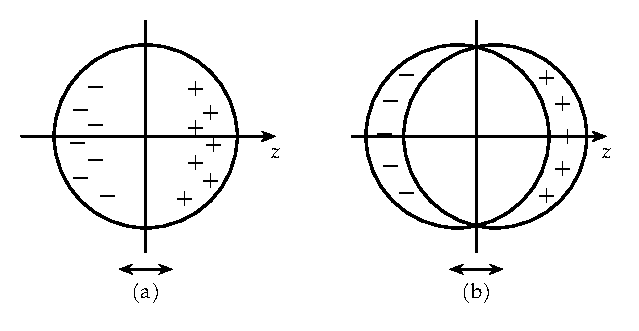
\includegraphics[width=0.7\textwidth]{pictures/13_10}
\par\end{centering}
\caption{\label{fig:13.10}图 13.10：球形核的偶极电极化模型示意图。减号代表质子缺陷（中子过剩），加号代表中子缺陷（质子过剩）。(a)
对应 Steinwedel-Jensen (SJ) 模型，(b) 对应 Goldhaber-Teller (GT) 模型。}
\end{figure}

在描述原子核巨偶极共振（GDR）等同位旋矢量激发（T=1 模式）时，历史上提出了两种著名的唯象流体动力学模型：

(1) Steinwedel-Jensen (SJ) 模型 \cite{SJ50}：假定原子核总体积与总核子密度严格保持不可压缩常数$\rho_{0}=\rho_{p}+\rho_{n}$，而质子流体与中子流体在固定的刚性核边界内发生反相相对密度振荡
{[}图 13.10(a){]}。定义相对密度差$\rho^{(1)}=\delta\rho_{p}-\delta\rho_{n}$，结合对称能变分推导出如下波动方程：

\[
\Delta\rho^{(1)}-\frac{1}{c^{2}}\frac{\partial^{2}\rho^{(1)}}{\partial t^{2}}=0,\quad c=\sqrt{\frac{2a_{\mathrm{sym}}}{m}}.
\]

在刚性核表面处无径向流出流的边界条件导出了特征偶极频率：

\[
\hbar\omega_{0}=2.08\frac{\hbar c}{R_{0}}\approx70\,A^{-1/3}\,\text{MeV}.
\]

(2) Goldhaber-Teller (GT) 模型 \cite{GT48}：假定质子流体球与中子流体球各自保持内部不可压缩，作为两个刚性刚球彼此反向平移相对振动
{[}图 13.10(b){]}。在 Tassie 表面振荡模型 \cite{Ta56a} 中，其跃迁密度完全集中在核表面弥散层，预言激发能随质量数呈$A^{-1/6}$的标度律。

\begin{figure}[H]
\begin{centering}
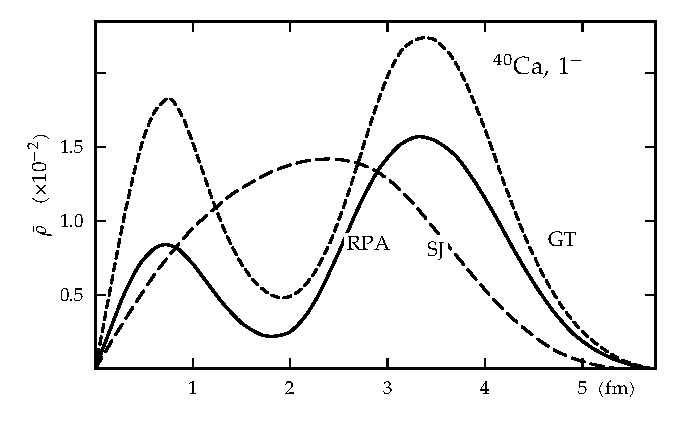
\includegraphics[width=0.65\textwidth]{pictures/13_11}
\par\end{centering}
\caption{\label{fig:13.11}图 13.11：$^{40}\text{Ca}$巨偶极态的跃迁密度对比。实线为基于微观 RPA
计算的最具集体性偶极态；虚线与点线分别代表 Goldhaber-Teller 模型与 Steinwedel-Jensen 模型的预言（引自
\cite{SR77}）。}
\end{figure}

从图 13.11 对比可见，在轻核$^{40}mathrm{Ca}$中，微观 RPA 的跃迁密度极其清晰地契合 GT 模型的表面峰化特征；而在重核中，SJ
体积振荡模式与 GT 表面位移模式则发生强烈混合 \cite{MSK77}。

\subsection{流体动力学的变分推导\label{subsec:13.3.4_=0053D8=005206=0063A8=005BFC}}

微观量子力学可以通过作用量的时间相关变分原理来严格导出。我们对多体态矢引入如下实虚部相因子分解拟设：

\[
|\Psi(t)\rangle=e^{\mathrm{i}S(t)}|\Phi_{0}(t)\rangle,
\]

假定相位算符由单粒子局域标量场决定，即对 Slater 行列式中所有单粒子轨道共享统一的空间相位$\phi_{i}(\boldsymbol{r},t)=e^{\mathrm{i}s(\boldsymbol{r},t)}\phi_{0i}(\boldsymbol{r},t)$。相应的流体速度场由相位梯度的无旋流严格给出：

\[
\boldsymbol{u}=\boldsymbol{\nabla}s.
\]

体系的总作用量积分泛函表述为经典的 Hamilton 形式，以局域密度与速度势构成正则共轭变量：

\[
I=\int\mathrm{d}t\int\mathrm{d}^{3}r\left\{ -m\dot{\rho}_{0}s-\frac{m}{2}\rho_{0}(\boldsymbol{\nabla}s)^{2}-\mathcal{E}[\rho_{0}]\right\} .
\]

变分方程直接导出连续性方程以及 Euler 形式的流体运动方程：

\[
\dot{\rho}_{0}=-\boldsymbol{\nabla}\cdot(\rho_{0}\boldsymbol{u}),
\]

\[
\frac{\partial\boldsymbol{u}}{\partial t}+(\boldsymbol{u}\cdot\boldsymbol{\nabla})\boldsymbol{u}=-\frac{1}{m}\boldsymbol{\nabla}\frac{\delta E_{\mathrm{int}}}{\delta\rho_{0}}.
\]


\subsection{密度 ρ₀ 的动量分布\label{subsec:13.3.5_=0052A8=0091CF=005206=005E03}}

在前面几节中我们数次指出：对于集体运动的流体动力学描述，将动量分布简单假定为球对称各向同性在绝大多数情况下并不成立。时间反演偶的密度矩阵$\rho_{0}$可表示为平衡密度矩阵通过厄米时间反演奇算符的变换$\rho_{0}=e^{\mathrm{i}\phi}\rho e^{-\mathrm{i}\phi}$。\footnote{这里的“静态”仅指时间以平庸的方式出现，即在每个瞬时外加约束不同，但我们均可求解一个瞬时定态（静态）Schrödinger 方程来计算$\rho_{0}${[}它不一定严格对应于该瞬时势中的基态密度
(参见第 12 章){]}。}当考虑无旋弱非局域流场时，展开至动量的一阶项：$\phi(\boldsymbol{q},\boldsymbol{p},t)=\boldsymbol{Q}(\boldsymbol{q},t)\cdot\boldsymbol{p}+\dots$。这一变换在物理几何上精确对应于将静态密度的空间坐标沿着含时位移矢量场进行局部仿射伸缩（scaling）。当原子核经历快速的集体振荡时，核子由于来不及通过频繁碰撞或能级跨越重新排布，Fermi
球将在相空间局域地发生严重的椭球形动量畸变\footnote{只有在体系激发能极高、核子平均自由程远小于核尺寸的极端高能重离子碰撞中，频繁的两体碰撞才会重新使动量分布恢复为各向同性。}。

\subsection{施加的流体动力学运动\label{subsec:13.3.6_=0065BD=0052A0=006D41=004F53=008FD0=0052A8}}

为了深入阐明动量畸变对集体激发的决定性影响，Holzwarth 和 Eckart \cite{HE78,HE79} 等学者研究了施加特定几何速度场时体系的自洽响应\footnote{另一个极其引人入胜的流场范例是所谓的扭动模（twist mode，参见第 8 章），其流场为$\boldsymbol{v}=(yz,-xz,0)$\cite{HE77,HE79}。在该模式下局域粒子数密度严格保持不变，唯有动量分布发生强烈的扭曲畸变。}。将位移场因子化为$\boldsymbol{Q}(\boldsymbol{r},t)=\alpha(t)\boldsymbol{v}(\boldsymbol{r})$，多极流场选取为：

\[
L=0:\boldsymbol{v}_{0}=\boldsymbol{r};\quad L=1:\boldsymbol{v}_{1}=\boldsymbol{\nabla}z;\quad L=2:\boldsymbol{v}_{2}=(-x,-y,2z)=\frac{1}{2}\boldsymbol{\nabla}(2z^{2}-x^{2}-y^{2}).
\]

对于四极模式（$L=2$），局域 Fermi 动量球面发生剧烈的四极形变：

\[
p^{2}_{F}(\theta,t)=p^{2}_{F}\left[1+2\alpha(t)P_{2}(\cos\theta)\right].
\]

动量球的非各向同性畸变直接给体系带来巨大的额外动能回跳弹性（恢复力常数）。动能对微扰参数$\alpha$的二阶微商给出的动能恢复力常数为：

\[
C_{T}=\left.\frac{\partial^{2}T_{\mathrm{dyn}}}{\partial\alpha^{2}}\right|_{\alpha=0}=\begin{cases}
4T_{0}, & L=0\\
0, & L=1\\
8T_{0}, & L=2
\end{cases}
\]

对于四极振动，总惯性质量参数为$B=2mA\langle r^{2}\rangle$，由此计算出的集体四极巨共振固有频率为：

\[
\hbar\Omega_{L=2}=\sqrt{\frac{4\langle T\rangle}{m\langle r^{2}\rangle}+\frac{C_{V}}{B}}\approx60\,A^{-1/3}\,\text{MeV}.
\]

这一理论预言与微观能量加权和规则 (8.167) 的精确结论惊人一致！经典普通液滴模型之所以在四极巨共振上给出完全错误的$A^{-1/2}$依赖律，其根本症结正在于彻底忽略了动态平均场边界对核子
Fermi 动量分布造成的体积各向异性畸变效应。而在偶极模式（L=1）中，由于流场与坐标无关，动量球保持刚性平移而不发生畸变；在单极呼吸模式（L=0）中，动量球各向同性均匀膨胀，普通流体力学与
Fermi 液体理论相吻合。这雄辩地证明：对于所有 L ≥ 2 的高阶多极表面集体振动，原子核必须被严格视为具有弹性切变回跳模量的量子
Fermi 液体，而非普通的经典流体。

\subsection{典型示例\label{subsec:13.3.7_=005178=00578B=00793A=004F8B}}

为了从理论上严格检验上述核流体动力学推导中所采用的基本假设，考察一个具有严格解析解的动力学微观模型是极具启发性的。假定初始核密度处于形变简谐振子势的基态，并在
t=0 时刻让其在球对称简谐振子势中开始自由演化。利用含时微观波函数 (10.89)，时间演化的密度矩阵严格表述为 \cite{BS79,SB79}：

\[
\rho(\boldsymbol{r},\boldsymbol{r}',t)=e^{\mathrm{i}\chi(\boldsymbol{r},t)}\rho_{0}(\boldsymbol{r},\boldsymbol{r}',t)e^{-\mathrm{i}\chi(\boldsymbol{r}',t)},
\]

其中瞬时流场势精确具有严格局域的形式：

\[
\chi(\boldsymbol{r},t)=\frac{m}{2}\frac{\mathrm{d}}{\mathrm{d}t}\left(\ln b_{x}x^{2}+\ln b_{y}y^{2}+\ln b_{z}z^{2}\right),
\]

且时间反演偶密度$\rho_{0}$完全由球形基态密度通过位移标度因子$\alpha_{j}(t)=-\ln b_{j}(t)$的刚性拉伸所严格给出。这一严格解析范例极其强有力地确证了核流体动力学核心假设在微观理论上的坚实立足点。


\part{Appendix}
\appendix


\chapter{实验室坐标系和体固坐标系中的角动量代数}

整本书我们都使用Edmonds\cite{Ed57}对于角动量耦合的约定和术语。唯一我们需要细细探究的地方就是如何把角动量转换到体坐标系。我们应当在Edmonds{[}Ed
57, Chap,IV{]}的意义下做这个转换。

为了研究Hilbert空间中的波函数在坐标系转动下的性质，我们应当首先考虑一个一维的例子
\begin{comment}
明明是二维。
\end{comment}
。

\begin{figure}[h]
\centering{}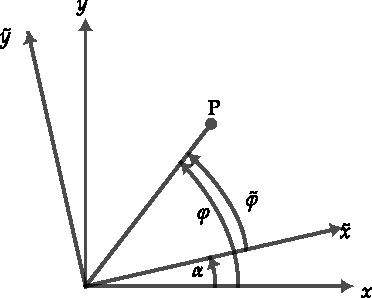
\includegraphics{pictures/绘图}
\end{figure}

令$f(\varphi)$是一个只依赖于相对于体系$z$轴的函数。在体系转动$\alpha$角后，空间中固定一点P对应的角$\varphi$变为角$\tilde{\varphi}=\varphi-\alpha$。因为函数$f$在固定点P的值在坐标系变换下不变，原坐标系中的函数$f$变成了新坐标系中的一个新函数$\tilde{f}$，具有性质：

\begin{equation}
\tilde{f}(\tilde{\varphi})=f(\varphi)=f(\tilde{\varphi}+\alpha)=\mathrm{e}^{\mathrm{i}\alpha J_{z}}f(\tilde{\varphi})
\end{equation}

或者，如果我们改变一下自变量
\begin{comment}
nomenclature不是这么翻译，我根据语境改的。
\end{comment}
，使用$\varphi$而不是$\tilde{\varphi}$，

\begin{equation}
\tilde{f}(\varphi)=\mathrm{e}^{\mathrm{i}\alpha J_{z}}f(\varphi)\quad\text{这里}J_{z}=\frac{1}{\mathrm{i}}\frac{\partial}{\partial\varphi}
\end{equation}

在三维旋转的情况，我们使用在\cite[Chap.I]{Ed57}中定义的Euler角$\Omega=(\alpha,\beta,\gamma)$：在转动了$\Omega$的情况下，波函数$|\Psi\rangle$变为：

\begin{equation}
|\tilde{\Psi}\rangle=R(\Omega)|\Psi\rangle\label{eq:=008F6C=0052A8=004E0B=006CE2=0051FD=006570=007684=0053D8=006362}
\end{equation}

这里酉旋转算符：

\begin{equation}
R(\Omega)=\mathrm{e}^{\mathrm{i}\alpha J_{z}}\mathrm{e}^{\mathrm{i}\beta J_{y}}\mathrm{e}^{\mathrm{i}\gamma J_{z}}
\end{equation}

这里$J_{x},J_{y},J_{z}$作用于坐标系$\boldsymbol{x}_{1},\dots,\boldsymbol{x}_{A}$上。正如在\cite{Ed57}中讨论的，我们也可以引入自旋。$\boldsymbol{J}$就是轨道角动量和自旋角动量的和。

和Hilbert空间中的矢量变换类似，我们可以得到一个算符$T$的变换：

\begin{equation}
T\rightarrow\tilde{T}=RTR^{\dagger}
\end{equation}

根据定义，对于一个球谐张量$T_{\lambda\mu}${[}Ed 57, Eq. (5.2.1){]}我们发现：

\begin{equation}
\tilde{T}_{\lambda\mu}=R(\Omega)T_{\lambda\mu}R^{\dagger}(\Omega)=\sum_{\mu^{\prime}}D^{\lambda}_{\mu^{\prime}\mu}(\Omega)T_{\lambda\mu^{\prime}}
\end{equation}

这里Wigner函数$D^{\lambda}_{\mu^{\prime}\mu}(\Omega)$可以给出：

\begin{equation}
D^{\lambda}_{\mu^{\prime}\mu}(\Omega)=\langle\lambda\mu^{\prime}|R(\Omega)|\lambda\mu\rangle
\end{equation}

我们现在希望研究在特定时间$t$从实验室坐标系到体固坐标系做的转动$\Omega$。记住角动量算符$J_{x},J_{y},J_{z}$是绕$x,y,z$轴无穷小转动的生成元，我们可以把这些算符表示为关于Euler角$\alpha,\beta,\gamma$的微分算符。例如，我们能通过改变Euler角$\alpha$一个$\delta\varphi$的小量而不改变体固坐标系得到绕$z$-轴$\delta\varphi$角的转动，也就是说：

\begin{equation}
L_{z}=-\frac{1}{\mathrm{i}}\frac{\partial}{\partial\alpha}\hat{=}J_{z}
\end{equation}

利用同样的方式，从Euler角的定义\cite{Ed57}中我们得到：

\begin{equation}
-\frac{1}{\mathrm{i}}\frac{\partial}{\partial\beta}\equiv J_{y^{\prime}}=\mathrm{e}^{\mathrm{i}\alpha J_{z}}J_{y}\mathrm{e}^{-\mathrm{i}\alpha J_{z}}=\cos\alpha J_{y}+\sin\alpha J_{x}
\end{equation}

和：

\begin{align}
-\frac{1}{\mathrm{i}}\frac{\partial}{\partial\gamma} & \equiv J_{z^{\prime\prime}}=\mathrm{e}^{\mathrm{i}\alpha J_{z}}\mathrm{e}^{\mathrm{i}\beta J_{y}}J_{z}\mathrm{e}^{-\mathrm{i}\beta J_{y}}\mathrm{e}^{-\mathrm{i}\alpha J_{z}}\nonumber \\
 & =\cos\beta J_{z}-\sin\beta(\cos\alpha J_{x}-\sin\alpha J_{y})
\end{align}

反解得到：

\begin{align}
L_{x} & \equiv\frac{1}{\mathrm{i}}\left(-\cos\alpha\cot\beta\frac{\partial}{\partial\alpha}-\sin\alpha\frac{\partial}{\partial\beta}+\frac{\cos\alpha}{\sin\beta}\frac{\partial}{\partial\gamma}\right)\hat{=}J_{x}\nonumber \\
L_{y} & \equiv\frac{1}{\mathrm{i}}\left(\sin\alpha\cot\beta\frac{\partial}{\partial\alpha}-\cos\alpha\frac{\partial}{\partial\beta}-\frac{\sin\alpha}{\sin\beta}\frac{\partial}{\partial\gamma}\right)\hat{=}J_{y}\\
L_{z} & \equiv\frac{1}{\mathrm{i}}\left(-\frac{\partial}{\partial\alpha}\right)\hat{=}J_{z}\nonumber 
\end{align}
 

它们是角动量



\chapter{电磁极矩与跃迁}

通过研究原子核在外部电磁场中的行为，我们可以了解核结构的信息。核与外场的相互作用是明确而简明
\begin{comment}
原文是广为人知的。
\end{comment}
的，因此这是一种获得原子核信息的好方法。许多作者推到了相关的公式，读者可以自行参阅它们以了解更多细节（例如{[}BW 52, Da
65a, SF 74{]}）。

\section{Hamilton量的基本形式}

一个原子核在一个外部电磁场中运动，这个外部电磁场被四维矢势$A_{\mu}=(\Phi,\boldsymbol{A})$或者电场$\boldsymbol{E}$和磁场$\boldsymbol{B}$所描述，Hamilton量写为：

\begin{equation}
H=H_{\text{nucl}}+H_{\text{field}}+H_{\text{int}}
\end{equation}

这里有三个部分：$H_{\text{nucl}}$是原子核的Hamilton量，或者至少是核模型的Hamilton量。我们假定我们知道它的本征函数$\Psi_{i}(1\dots A)$：

\begin{equation}
H_{\text{nucl}}=\Psi_{i}(1\dots A)=E_{i}\Psi_{i}(1\dots A)
\end{equation}

$H_{\text{field}}$可以如下给出：

\begin{equation}
H_{\text{field}}=\frac{1}{8\mathrm{\pi}}\int\left(\boldsymbol{E}^{2}(\boldsymbol{r},t)+\boldsymbol{B}^{2}(\boldsymbol{r},t)\right)\,\mathrm{d}^{3}\boldsymbol{r}
\end{equation}

外场和原子核的相互作用可以写为
\begin{comment}
第一项的$c$去哪儿了？
\end{comment}
：

\begin{equation}
H_{\text{int}}=-\frac{1}{c}\int j_{\mu}A^{\mu}\,\mathrm{d^{3}\boldsymbol{r}=\int\left(\rho(\boldsymbol{r},t)\Phi(\boldsymbol{r},t)-\frac{1}{c}\boldsymbol{j}(\boldsymbol{r},t)\cdot\boldsymbol{A}(\boldsymbol{r},t)\right)\,\mathrm{d}^{3}\boldsymbol{r}}
\end{equation}

这里$\rho(\boldsymbol{r},t)$是核电荷密度：

\begin{equation}
\rho(\boldsymbol{r},t)=\sum^{A}_{i=1}e\left(\frac{1}{2}-t^{(i)}_{3}\right)\cdot\delta(\boldsymbol{r}-\boldsymbol{r}_{i}(t))
\end{equation}

这里我们把核子当成了点粒子。事实上，它们有一个有限的延展，可以由形状因子给出。这在{[}BM69, App.3C{]}中有着简单的介绍，出于简明性的考虑我们这里暂时不去考虑它。

原子核中的电流密度$\boldsymbol{j}(\boldsymbol{r},t)$和磁矩密度有关
\begin{comment}
这个关系是咋来的啊，忘干净了。
\end{comment}
：

\begin{equation}
\boldsymbol{j}(\boldsymbol{r},t)=c\nabla\times\boldsymbol{\mu}(\boldsymbol{r},t)
\end{equation}

它有两部分
\begin{comment}
这个两部分并不是都用$\boldsymbol{j}$或者$\boldsymbol{\mu}$表示出来的就让人很难受。但是没办法，这是为了后面方便计算。
\end{comment}
：
\begin{enumerate}
\item 轨道部分，来自于移动的质子：

\begin{equation}
j^{o}(\boldsymbol{r},t)=\sum^{A}_{i=1}e\left(\frac{1}{2}-t^{(i)}_{3}\right)\frac{1}{2}(\boldsymbol{v}_{i}\delta(\boldsymbol{r}-\boldsymbol{r}_{i}(t)+\text{h.c.})
\end{equation}

$\boldsymbol{v}_{i}$可以如下给出：

\begin{equation}
\boldsymbol{v}_{i}=\frac{\mathrm{i}}{\hbar}[H,\boldsymbol{r}_{i}]
\end{equation}

对于速度无关的势，我们有$\boldsymbol{v}_{i}=(1/m)\boldsymbol{p}_{i}$
\begin{comment}
于是有：
\[
j^{o}(\boldsymbol{r},t)=\sum^{A}_{i=1}e\left(\frac{1}{2}-t^{(i)}_{3}\right)\boldsymbol{v}_{i}\delta(\boldsymbol{r}-\boldsymbol{r}_{i}(t)
\]

然而在核物理中这是否只是美好的期望？
\end{comment}
。接下来我们仅仅考虑这种情况。此外，这里没有考虑$\pi$介子交换流，更细节的讨论可见\cite{SF74}。
\item 自旋部分，它来自于原子核的自旋分布，可以如下给出：

\begin{equation}
\boldsymbol{\mu}^{s}(\boldsymbol{r},t)=\sum^{A}_{i=1}\delta(\boldsymbol{r}-\boldsymbol{r}_{i}(t))\frac{e\hbar}{2mc}\left\{ \left(\frac{1}{2}-t^{(i)}_{3}\right)g_{p}+\left(\frac{1}{2}+t^{(i)}_{3}\right)g_{n}\right\} \boldsymbol{s}_{i}
\end{equation}

这里$g_{p}$和$g_{n}$是自由质子和中子的$g$-因子（$g_{p}=5.586$，$g_{n}=-3.826$）。$\pi$介子交换流有时可以通过使用有效$g$-因子加以考虑。接下来，我们使用核磁子$\mu_{N}=e\hbar/2mc$。
\end{enumerate}

\section{静态多极矩}

和静态的电磁场的相互作用会导致核能级的改变，在一阶微扰论下，第$i$个能级的改变量为：

\begin{equation}
\Delta E_{i}=\langle\Psi_{i}|H_{\text{int}}|\Psi\rangle
\end{equation}

我们引入磁通量密度
\begin{comment}
这不就是磁场吗？怎么就磁通量密度了？
\end{comment}
$\boldsymbol{B}=\nabla\times\boldsymbol{A}$，可以得到：

\begin{equation}
H_{\text{int}}=\int\rho(\boldsymbol{r})\Phi(\boldsymbol{r})\,\mathrm{d}^{3}\boldsymbol{r}-\int\boldsymbol{\mu}(\boldsymbol{r})\cdot\boldsymbol{B}(\boldsymbol{r})\,\mathrm{d}^{3}\boldsymbol{r}
\end{equation}

\begin{booknote*}
首先利用求和记号：

\begin{align*}
\boldsymbol{j}\cdot\boldsymbol{A} & =c(\nabla\times\boldsymbol{\mu})\cdot\boldsymbol{A}\\
 & =c\varepsilon_{ijk}(\partial_{j}\mu_{k})A_{i}\\
 & =c\varepsilon_{ijk}(\partial_{j}\mu_{k}A_{i})-c\varepsilon_{ijk}\mu_{k}(\partial_{j}A_{i})\\
 & =c\nabla\cdot(\boldsymbol{\mu}\times\boldsymbol{A})-c\boldsymbol{\mu}\cdot\boldsymbol{B}
\end{align*}

积分，得到：

\begin{align*}
-\frac{1}{c}\int\boldsymbol{j}\cdot\boldsymbol{A}\,\mathrm{d}^{3}\boldsymbol{r} & =-\int\nabla\cdot(\boldsymbol{\mu}\times\boldsymbol{A})\,\mathrm{d}^{3}\boldsymbol{r}+\int\boldsymbol{\mu}\cdot\boldsymbol{B}\,\mathrm{d}^{3}\boldsymbol{r}\\
 & =-\int\boldsymbol{\mu}(\boldsymbol{r})\cdot\boldsymbol{B}(\boldsymbol{r})\,\mathrm{d}^{3}\boldsymbol{r}
\end{align*}

这里省去了第一项，原因是$\mu(\boldsymbol{r})$在边界处显然为零。
\end{booknote*}
由于外场的源和原子核相距很远，因此原子核中的$\Phi(\boldsymbol{r})$和$\boldsymbol{B}(\boldsymbol{r})$满足均匀Maxwell方程组：

\begin{align}
\nabla^{2}\Phi(\boldsymbol{r}) & =0\nonumber \\
\nabla\times\boldsymbol{B}(\boldsymbol{r}) & =0\\
\nabla\cdot\boldsymbol{B}(\boldsymbol{r}) & =0\nonumber 
\end{align}

这意味着$\boldsymbol{B}$可以写成：

\begin{equation}
\boldsymbol{B}(\boldsymbol{r})=-\nabla\Xi(\boldsymbol{r})
\end{equation}

并且有：

\begin{equation}
\nabla^{2}\Xi(\boldsymbol{r})=0
\end{equation}

在球坐标系，上面两个拉普拉斯方程的最一般的在原点处不发散的解可以写为：

\begin{align}
\Phi(\boldsymbol{r}) & =\sum_{\lambda\mu}a_{\lambda\mu}r^{\lambda}Y_{\lambda\mu}(\theta,\phi)\\
\Xi(\boldsymbol{r}) & =\sum_{\lambda\mu}b_{\lambda\mu}r^{\lambda}Y_{\lambda\mu}(\theta,\phi)
\end{align}

这里$Y_{\lambda\mu}$是球谐函数。

我们发现：

\begin{equation}
H_{\text{int}}=\sum_{\lambda\mu}a_{\lambda\mu}\hat{Q}_{\lambda\mu}+b_{\lambda\mu}\hat{M}_{\lambda\mu}
\end{equation}

这里电磁多极算符为：

\begin{align}
\hat{Q}_{\lambda\mu} & =\int\rho(\boldsymbol{r})r^{\lambda}Y_{\lambda\mu}(\theta,\phi)\,\mathrm{d}^{3}\boldsymbol{r}\\
\hat{M}_{\lambda\mu} & =\int\boldsymbol{\mu}(\boldsymbol{r})\cdot\nabla(r^{\lambda}Y_{\lambda\mu}(\theta,\phi))\,\mathrm{d}^{3}\boldsymbol{r}
\end{align}

在代入$\rho(\boldsymbol{r})$和$\boldsymbol{\mu}(\boldsymbol{r})$的具体形式之前，我们可以把$\hat{M}_{\lambda\mu}$重写一下。

我们需要用到关系
\begin{comment}
这里我不知道该用什么符号让它清楚一点。
\end{comment}
：

\begin{equation}
\nabla\times[\nabla\times(r^{\lambda}Y_{\lambda\mu}(\theta,\phi)\boldsymbol{r})]=(\lambda+1)\nabla(r^{\lambda}Y_{\lambda\mu}(\theta,\phi))
\end{equation}

\begin{booknote*}
证明。首先利用：

\[
\nabla\times\nabla\times*=\nabla[\nabla\cdot*]-\nabla^{2}*
\]

得到：

\[
\nabla[\nabla\cdot(r^{\lambda+1}Y_{\lambda\mu}(\theta,\phi)\hat{\boldsymbol{e}}_{r})]-\nabla^{2}(r^{\lambda}Y_{\lambda\mu}(\theta,\phi)\boldsymbol{r})
\]

第一项可以利用球坐标散度形式得到为：

\[
(\lambda+3)\nabla(r^{\lambda}Y_{\lambda\mu}(\theta,\phi))
\]

第二项为：

\begin{align*}
\partial_{j}\partial_{j}(r^{\lambda}Y_{\lambda\mu}r_{i}) & =\partial_{j}[\partial_{j}(r^{\lambda}Y_{\lambda\mu})r_{i}+r^{\lambda}Y_{\lambda\mu}\partial_{j}r_{i}]\\
 & =\partial^{2}(r^{\lambda}Y_{\lambda\mu})r_{i}+2\partial_{j}(r^{\lambda}Y_{\lambda\mu})\partial_{j}r_{i}+r^{\lambda}Y_{\lambda\mu}\partial^{2}r_{i}
\end{align*}

我们显然有$\partial^{2}(r^{\lambda}Y_{\lambda\mu})=0$，也有$\partial^{2}r_{i}=0$，因此得到：

\[
\partial_{j}\partial_{j}(r^{\lambda}Y_{\lambda\mu}r_{i})=2\partial_{i}(r^{\lambda}Y_{\lambda\mu})
\]

两项相加，得：

\[
\nabla\times\nabla\times(r^{\lambda}Y_{\lambda\mu}(\theta,\phi)\boldsymbol{r})=(\lambda+1)\nabla\left(r^{\lambda}Y_{\lambda\mu}(\theta,\phi)\right)
\]
\end{booknote*}
把这一关系代入$\hat{M}_{\lambda\mu}$的表达式中，分部积分，得：

\begin{align}
\hat{M}_{\lambda\mu} & =\frac{1}{\lambda+1}\int[\boldsymbol{r}\times(\nabla\times\boldsymbol{\mu}(\boldsymbol{r}))]\cdot\nabla(r^{\lambda}Y_{\lambda\mu})\,\mathrm{d}^{3}\boldsymbol{r}\\
 & =\frac{1}{c(\lambda+1)}\int(\boldsymbol{r}\times\boldsymbol{j}(\boldsymbol{r}))\cdot\nabla(r^{\lambda}Y_{\lambda\mu})\,\mathrm{d}^{3}\boldsymbol{r}\label{eq:=009759=006001=0078C1=00591A=006781=0077E9}
\end{align}

\begin{booknote*}
代入，得：

\[
\hat{M}_{\lambda\mu}=\frac{1}{\lambda+1}\int\boldsymbol{\mu}(\boldsymbol{r})\cdot\nabla\times[\nabla\times(r^{\lambda}Y_{\lambda\mu}(\theta,\phi)\boldsymbol{r})]\,\mathrm{d}^{3}\boldsymbol{r}
\]

分部积分一次，得：

\begin{align*}
\hat{M}_{\lambda\mu} & =\frac{1}{\lambda+1}\int[\nabla\times\boldsymbol{\mu}(\boldsymbol{r})]\cdot[\nabla\times(r^{\lambda}Y_{\lambda\mu}(\theta,\phi)\boldsymbol{r})]\,\mathrm{d}^{3}\boldsymbol{r}
\end{align*}

接下来，利用$\nabla\times(f\boldsymbol{r})=(\nabla f)\times\boldsymbol{r}$，得到：

\[
\hat{M}_{\lambda\mu}=\frac{1}{\lambda+1}\int[\nabla\times\boldsymbol{\mu}(\boldsymbol{r})]\cdot[\nabla(r^{\lambda}Y_{\lambda\mu}(\theta,\phi)\times\boldsymbol{r})]\,\mathrm{d}^{3}\boldsymbol{r}
\]

再利用$\boldsymbol{a}\cdot(\boldsymbol{b}\times\boldsymbol{c})=(\boldsymbol{c}\times\boldsymbol{a})\cdot\boldsymbol{b}$，得：

\[
\hat{M}_{\lambda\mu}=\frac{1}{\lambda+1}\int[\boldsymbol{r}\times(\nabla\times\boldsymbol{\mu}(\boldsymbol{r}))]\cdot\nabla(r^{\lambda}Y_{\lambda\mu}(\theta,\phi))\,\mathrm{d}^{3}\boldsymbol{r}
\]
\end{booknote*}
现在把$\rho(\boldsymbol{r})$和$\boldsymbol{\mu}(\boldsymbol{r})$的表达式代入，并且发现$\boldsymbol{l}_{i}=(1/\mathrm{i})(\boldsymbol{r}_{i}\times\nabla_{i})$，得：

\begin{align}
\hat{Q}_{\lambda\mu} & =e\sum^{A}_{i=1}\left(\frac{1}{2}-t^{(i)}_{3}\right)r^{\lambda}_{i}Y_{\lambda\mu}(\theta_{i},\phi_{i})\label{eq:=009759=006001=007535=00591A=006781=007B97=007B26=005177=004F53}\\
\hat{M}_{\lambda\mu} & =\mu_{N}\sum^{A}_{i=1}\left\{ g^{(i)}_{s}\boldsymbol{s}_{i}+\frac{2}{\lambda+1}\cdot g^{(i)}_{l}\boldsymbol{l}_{i}\right\} \cdot\nabla(r^{\lambda}Y_{\lambda\mu}(\theta,\phi))_{r=r_{i}}\label{eq:=009759=006001=0078C1=00591A=006781=007B97=007B26=005177=004F53}
\end{align}

这里：

\[
\left.\begin{array}{c}
g^{(i)}_{s}=g_{p}\\
g^{(i)}_{l}=1
\end{array}\right\} \quad\text{对质子来说}\quad\left.\begin{array}{c}
g^{(i)}_{s}=g_{n}\\
g^{(i)}_{l}=0
\end{array}\right\} \quad\text{对中子来说}
\]

此外，算符$\boldsymbol{l}_{i}$仅仅作用在$\boldsymbol{r}_{i}$上。它与$\nabla r^{\lambda}Y_{\lambda\mu}$对易：

\begin{equation}
\boldsymbol{l}\cdot(\nabla r^{\lambda}Y_{\lambda\mu})\propto(\boldsymbol{r}\times\nabla)\cdot\nabla r^{\lambda}Y_{\lambda\mu}=\boldsymbol{r}\cdot(\nabla\times\nabla)r^{\lambda}Y_{\lambda\mu}=0
\end{equation}

\begin{booknote*}
首先看电多极算符：

\begin{align*}
\hat{Q}_{\lambda\mu} & =e\sum^{A}_{i=1}\left(\frac{1}{2}-t^{(i)}_{3}\right)\int\delta(\boldsymbol{r}-\boldsymbol{r}_{i}(t))r^{\lambda}Y_{\lambda\mu}(\theta,\phi)\,\mathrm{d}^{3}\boldsymbol{r}\\
 & =e\sum^{A}_{i=1}\left(\frac{1}{2}-t^{(i)}_{3}\right)r^{\lambda}_{i}Y_{\lambda\mu}(\theta_{i},\phi_{i})
\end{align*}

磁多极算符分为两部分，第一部分是：

\begin{align*}
\hat{M}^{o}_{\lambda\mu} & =\frac{1}{c(\lambda+1)}\int(\boldsymbol{r}\times\boldsymbol{j}^{o}(\boldsymbol{r}))\cdot\nabla(r^{\lambda}Y_{\lambda\mu})\,\mathrm{d}^{3}\boldsymbol{r}\\
 & =\mu_{N}\frac{2}{\lambda+1}\sum^{A}_{i=1}g^{(i)}_{l}(\frac{m}{\mathrm{i}\hbar}\boldsymbol{r}_{i}\times\boldsymbol{v}_{i})\cdot\nabla(r^{\lambda}Y_{\lambda\mu}(\theta,\phi))_{r=r_{i}}\\
 & =\mu_{N}\frac{2}{\lambda+1}\sum^{A}_{i=1}g^{(i)}_{l}\boldsymbol{l}_{i}\cdot\nabla(r^{\lambda}Y_{\lambda\mu}(\theta,\phi))_{r=r_{i}}
\end{align*}

第二部分是：

\begin{align*}
\hat{M}^{s}_{\lambda\mu} & =\int\boldsymbol{\mu}^{s}(\boldsymbol{r})\cdot\nabla(r^{\lambda}Y_{\lambda\mu}(\theta,\phi))\,\mathrm{d}^{3}\boldsymbol{r}\\
 & =\mu_{N}\sum^{A}_{i=1}g^{(i)}_{s}\boldsymbol{s}_{i}\cdot\nabla(r^{\lambda}Y_{\lambda\mu}(\theta,\phi))_{\boldsymbol{r}=\boldsymbol{r}_{i}}
\end{align*}

相加即得：

\[
\hat{M}_{\lambda\mu}=\mu_{N}\sum^{A}_{i=1}\left\{ g^{(i)}_{s}\boldsymbol{s}_{i}+\frac{2}{\lambda+1}\cdot g^{(i)}_{l}\boldsymbol{l}_{i}\right\} \cdot\nabla(r^{\lambda}Y_{\lambda\mu}(\theta,\phi))_{r=r_{i}}
\]
\end{booknote*}
这些算符在态$|\Psi\rangle$上的期待值就是这个态的电或磁矩：

\begin{align}
Q_{\lambda\mu} & =\langle\Psi|\hat{Q}_{\lambda\mu}|\Psi\rangle\\
M_{\lambda\mu} & =\langle\Psi|\hat{M}_{\lambda\mu}|\Psi\rangle
\end{align}

我们首先讨论$Q_{\lambda\mu}$和$M_{\lambda\mu}$的选择定则，因为它们和态$|\Psi\rangle$具体的形式无关。由于强相互作用和电磁相互作用宇称守恒，选择$|\Psi\rangle$是宇称算符的本征态是合理的。另一方面，多极算符$\hat{Q}_{\lambda\mu}$和$\hat{M}_{\lambda\mu}$分别具有$(-)^{\lambda}$和$(-)^{\lambda+1}$的宇称。这意味着：

\begin{align}
Q_{\lambda\mu} & =0\quad\text{对}\lambda=1,3,5,\dots\nonumber \\
M_{\lambda\mu} & =0\quad\text{对}\lambda=0,2,4,\dots
\end{align}

利用算符$\hat{Q}_{\lambda\mu}$和$\hat{M}_{\lambda\mu}$是球谐张量，我们可以对角动量本征态$|I,M\rangle$使用Wigner-Eckart定理：

\begin{align}
Q_{\lambda\mu} & =\langle IM|\hat{Q}_{\lambda\mu}|IM\rangle=(-)^{I-M}\begin{pmatrix}I & \lambda & I\\
-M & \mu & M
\end{pmatrix}\langle I||\hat{Q}_{\lambda}||I\rangle\\
M_{\lambda\mu} & =\langle IM|\hat{M}_{\lambda\mu}|IM\rangle=(-)^{I-M}\begin{pmatrix}I & \lambda & I\\
-M & \mu & M
\end{pmatrix}\langle I||\hat{M}_{\lambda\mu}||I\rangle\nonumber 
\end{align}

由此得到：

\begin{equation}
\left.\begin{array}{c}
Q_{\lambda\mu}\\
M_{\lambda\mu}
\end{array}\right\} \neq0\quad\text{仅仅对}\mu=0\text{和}0\leq\lambda\leq2I\text{成\text{立}}
\end{equation}

由于$Q_{\lambda\mu}$和$M_{\lambda\mu}$关于磁量子数的关系是平凡的，我们往往只给出$M=I$的值。

磁偶极矩被定义为：

\begin{equation}
\boldsymbol{\mu}=\sqrt{\frac{4\mathrm{\pi}}{3}}\langle II|\hat{M}_{10}|II\rangle
\end{equation}

电偶极矩被定义为：

\begin{equation}
Q=\sqrt{\frac{16\mathrm{\pi}}{5}}\langle II|\hat{Q}_{20}|II\rangle
\end{equation}

这些值是在实验室系下定义的并且可以被实验测量。内禀的多极矩可以由1.70
\begin{comment}
还没写，之后再说。
\end{comment}
给出。

\section{辐射场的多级展开}

在电磁辐射的情况下，使用Coulomb规范是方便的：

\begin{equation}
\Phi=0;\quad\nabla\cdot\boldsymbol{A}=0\label{eq:Coulomb=0089C4=008303}
\end{equation}

自由场的Hamilton量可以写为：

\begin{equation}
H_{\text{field}}=\frac{1}{8\mathrm{\pi}}\int\left(\frac{1}{c^{2}}\dot{\boldsymbol{A}}^{2}+(\nabla\times\boldsymbol{A})^{2}\right)\,\mathrm{d}^{3}\boldsymbol{r}
\end{equation}

由此可以推出波动方程：

\begin{equation}
\nabla^{2}\boldsymbol{A}-\frac{1}{c^{2}}\frac{\partial^{2}}{\partial t^{2}}\boldsymbol{A}=0
\end{equation}

为了表示出最一般的矢势$\boldsymbol{A}$，我们需要找一组满足上述方程的完备正交基。此时，我们通常做时间与空间的Fourier变换，然后只保留与波矢$\boldsymbol{k}$垂直的部分以满足\ref{eq:Coulomb=0089C4=008303}。
\begin{comment}
虽然没搞懂它在说什么，不过应该不重要。
\end{comment}
然而，此处有球对称，我们只做时间的Fourier变换，也就是说，我们假设我们的基关于时间的依赖是$\exp(-\mathrm{i}kct)$，并且满足Helmholtz方程：

\begin{equation}
(\nabla^{2}+k^{2})\boldsymbol{A}=0
\end{equation}

\begin{comment}
下面这一段其实只是找到解，没必要看。可以直接跳到$\boldsymbol{A}$的一般形式。
\end{comment}
根据球对称性，我们可以使用轨道角动量$\boldsymbol{L}^{2}$和$L_{z}$的本征函数。一组满足这一条件并且在原点处不发散的基是$j_{L}(kr)Y_{LM_{L}}(\theta,\phi)$，这里$j_{L}(kr)$是球Bessel函数，$Y_{LM}$是球谐函数。除了轨道角动量，根据$\boldsymbol{A}$的矢量性质，光子还应具有$1$自旋，即$S=1$。$\boldsymbol{S}^{2}$和$S_{z}$的本征函数是矢量$\boldsymbol{e}_{M_{S}}$（$M_{S}=+1,0,-1$）。光子的总角动量可以由$\boldsymbol{I}=\boldsymbol{L}+\boldsymbol{S}$给出。根据角动量耦合规则，我们可以使用$\boldsymbol{L}^{2}$，$\boldsymbol{S}^{2}$，$\boldsymbol{I}^{2}$，$I_{z}$的本征函数，即矢量球谐函数：

\begin{equation}
\boldsymbol{Y}_{ILM}(\Omega)=\sum_{M_{S}M_{L}}C^{L1I}_{M_{L}M_{S}m}Y_{LM_{L}}(\Omega)\boldsymbol{e}_{M_{S}}
\end{equation}

它们组成了一组完备正交基：

\[
\int\mathrm{d}\Omega\,\boldsymbol{Y}^{*}_{ILm}(\Omega)\boldsymbol{Y}_{I^{\prime}L^{\prime}m^{\prime}}(\Omega)=\delta_{ll^{\prime}}\delta_{LL^{\prime}}\delta_{mm^{\prime}}
\]

对于固定的$I$，轨道角动量可以是$I-1$，$I$，$I+1$。这意味着Helmholtz方程对于每个$k$，$I$，$m$可以有三个独立的解
\begin{comment}
这里应该对应三种矢量球谐函数？
\end{comment}
。然而我们还必须要满足\ref{eq:Coulomb=0089C4=008303}。

从{[}Ed. 57{]}可知
\begin{comment}
已查阅，证明复杂，等着写了角动量部分再说。
\end{comment}
：

\begin{equation}
\boldsymbol{Y}_{IIm}(\Omega)=\frac{1}{\sqrt{I(I+1)}}\boldsymbol{L}Y_{Im}(\Omega)\label{eq:=0077E2=0091CF=007403=008C10=0051FD=006570=007B80=00660E=005199=006CD5}
\end{equation}

我们可以发现，$j_{I}(kr)\boldsymbol{Y}_{IIm}(\Omega)$
\begin{comment}
原书上这个地方应该是写错了。
\end{comment}
自动满足\ref{eq:Coulomb=0089C4=008303}。上式的正交波函数是$\boldsymbol{Y}_{I,I+1,m}$和$\boldsymbol{Y}_{I,I-1,m}$。只有一个这样的组合满足\ref{eq:Coulomb=0089C4=008303}：

\begin{equation}
\frac{\mathrm{i}}{k}\nabla\times(j_{l}(kr)\boldsymbol{Y}_{IIm})=\sqrt{\frac{I}{2I+1}}j_{I+1}(kr)\boldsymbol{Y}_{I,I+1,m}-\sqrt{\frac{I+1}{2I+1}}j_{I-1}(kr)\boldsymbol{Y}_{I,I-1,m}
\end{equation}

\begin{booknote*}
验证$j_{I}(kr)\boldsymbol{Y}_{IIm}(\Omega)$满足Coulomb规范，首先证明：

\begin{align*}
\nabla\cdot\left(j_{I}(kr)\boldsymbol{r}\times\nabla Y_{IIm}(\Omega)\right) & =\boldsymbol{r}\cdot\left(\nabla j_{I}(kr)\times\nabla Y_{IIm}(\Omega)\right)
\end{align*}

由于$\nabla j_{I}(kr)$与$\boldsymbol{r}$方向相同，可以得到其为零。
\end{booknote*}
因此，对每个$I$和$m$，我们得到了Helmholtz方程满足\ref{eq:Coulomb=0089C4=008303}的两个独立的解。我们用一个指标$\lambda$标记他们并称它们为电（$\lambda=E$）和磁（$\lambda=M$）辐射：

\begin{align}
\boldsymbol{A}_{MkIm} & (\boldsymbol{r})=\mathcal{N}j_{I}(kr)\boldsymbol{Y}_{IIm}(\Omega)\nonumber \\
 & =\frac{\mathcal{N}}{\sqrt{I(I+1)}}\frac{1}{\mathrm{i}}(\boldsymbol{r}\times\nabla)j_{I}(kr)Y_{Im}(\Omega)
\end{align}

和：

\begin{align}
\boldsymbol{A}_{EkIm}(\boldsymbol{r}) & =\frac{\mathrm{i}}{k}(\nabla\times\boldsymbol{A}_{MkIm}(\boldsymbol{r}))\nonumber \\
 & =\frac{-\mathcal{N}}{\sqrt{I(I+1)}}\frac{1}{k}\left\{ \nabla\left[Y_{Im}(\Omega)\frac{\partial}{\partial r}(rj_{I}(kr))\right]+k^{2}\boldsymbol{r}j_{I}(kr)Y_{Im}(\Omega)\right\} 
\end{align}

电辐射解是从磁辐射解中得到的，过程中计算了$\nabla\times\nabla\times(\boldsymbol{r}j_{I}Y_{Im})$并且利用了$j_{I}Y_{Im}$满足Helmholtz方程的事实。
\begin{booknote*}
将$\boldsymbol{A}_{MkIm}$代入，得：

\begin{align*}
\boldsymbol{A}_{EkIm}(\boldsymbol{r}) & =\frac{\mathrm{i}}{k}(\nabla\times\boldsymbol{A}_{MkIm}(\boldsymbol{r}))\\
 & =\frac{\mathcal{N}}{\sqrt{I(I+1)}}\frac{1}{k}\nabla\times\bigl[\boldsymbol{r}\times\nabla\bigl(j_{I}(kr)Y_{Im}(\Omega)\bigr)\bigr]\\
 & =\frac{-\mathcal{N}}{\sqrt{I(I+1)}}\frac{1}{k}\nabla\times\bigl[\nabla\times\bigl(\boldsymbol{r}j_{I}(kr)Y_{Im}(\Omega)\bigr)\bigr]
\end{align*}

利用矢量分析公式：

\[
\nabla\times\bigl[\nabla\times\bigl(\boldsymbol{r}*\bigr)\bigr]=\nabla\bigl[\nabla\cdot(\boldsymbol{r}*)\bigr]-\nabla^{2}(\boldsymbol{r}*)
\]

对于第一项，利用球坐标的梯度公式，得到：

\[
\nabla\bigl[\nabla\cdot(\boldsymbol{r}*)\bigr]=\nabla\left[\frac{1}{r^{2}\sin\theta}\frac{\partial}{\partial r}(r^{2}\sin\theta\cdot r*)\right]=\nabla\left[\frac{\partial}{\partial r}(r*)\right]+2\nabla(*)
\]

对于第二项，利用矢量分析公式：

\begin{align*}
\nabla^{2}(\boldsymbol{r}*) & =2\nabla(*)+\boldsymbol{r}\nabla^{2}(*)
\end{align*}

于是得到：

\[
\nabla\times\bigl[\nabla\times\bigl(\boldsymbol{r}*\bigr)\bigr]=\nabla\left[\frac{\partial}{\partial r}(r*)\right]-\boldsymbol{r}\nabla^{2}(*)
\]

利用Helmholtz方程，则可得到：

\[
\boldsymbol{A}_{EkIm}(\boldsymbol{r})=\frac{-\mathcal{N}}{\sqrt{I(I+1)}}\frac{1}{k}\left\{ \nabla\left[Y_{Im}(\Omega)\frac{\partial}{\partial r}(rj_{I}(kr))\right]+k^{2}\boldsymbol{r}j_{I}(kr)Y_{Im}(\Omega)\right\} 
\]
\end{booknote*}
$\mathcal{N}$是归一化系数。量子数$k$通过在半径为 $R$的完美导体球面上要求适当的边界条件来离散化。球面的引入仅仅是为了引入边界条件，在最后需要让其远大于核半径$R_{0}$。根据经典电动力学，边界条件应当为$E_{\parallel}=0$和$B_{\perp}=0$。这些条件只有当$k$值是离散的值$k_{n}$的时候才能满足。在磁的情况下他们可以由Bessel函数的零点给出：

\begin{equation}
j_{I}(k_{n}R)=0\label{eq:=0078C1=008FB9=00754C=006761=004EF6}
\end{equation}

在电的情况下，条件为：

\begin{equation}
\left.\frac{\partial}{\partial r}(rj_{I}(k_{n}r))\right|_{r=R}=0
\end{equation}

接下来我们把$k$当做离散指标，取遍所有可能的离散值。

归一化系数$\mathcal{N}$选取为使得如下正交关系满足的值：

\begin{equation}
\int^{R}_{0}r^{2}\mathrm{d}r\int\mathrm{d}\Omega\,\boldsymbol{A}^{*}_{\lambda^{\prime}k^{\prime}I^{\prime}m^{\prime}}(\boldsymbol{r})\cdot\boldsymbol{A}_{\lambda kIm}(\boldsymbol{r})=\frac{2\mathrm{\pi}\hbar c}{k}\delta_{\lambda\lambda^{\prime}}\delta_{kk^{\prime}}\delta_{II^{\prime}}\delta_{mm^{\prime}}
\end{equation}

在大$R$极限下，$\mathcal{N}$被证明是：

\begin{equation}
\mathcal{N}=\sqrt{\frac{4\mathrm{\pi}\hbar ck}{R}}
\end{equation}

这在两种$\lambda$的情况下都成立。

电磁辐射在宇称变换下的性质可以由\ref{eq:=0077E2=0091CF=007403=008C10=0051FD=006570=007B80=00660E=005199=006CD5}得到。角动量算符$\boldsymbol{L}$保持宇称，而旋度算符改变宇称，于是得到：

\begin{align}
\Pi\boldsymbol{A}_{EkIm} & =(-)^{I+1}\boldsymbol{A}_{EkIm}\nonumber \\
\Pi\boldsymbol{A}_{MkIm} & =(-)^{I}\boldsymbol{A}_{MkIm}\label{eq:=007535=0078C1=008F90=005C04=005728=005B87=0079F0=0053D8=006362=004E0B=006027=008D28}
\end{align}

于是我们这个问题的最一般的解为：

\begin{equation}
\boldsymbol{A}(\boldsymbol{r},t)=\sum_{\lambda k}\sum_{Im}\left(a^{*}_{\lambda kIm}\boldsymbol{A}_{\lambda kIm}(\boldsymbol{r})\mathrm{e}^{-\mathrm{i}kct}+\text{c.c.}\right)
\end{equation}

系数$a_{\lambda kIm}$是描述电磁场$\boldsymbol{A}$的独立变量。上面这种形式保证了选取任意$a_{\lambda kIm}$都能使得Coulomb规范和Helmholtz方程被满足。

利用正交关系，我们可以把自由场Hamilton量表示为
\begin{comment}
这里$a$是数的情况下本可以简写为$H_{\text{field}}=\sum_{\lambda k}\sum_{Im}\hbar cka^{*}_{\lambda kIm}a_{\lambda kIm}$，但为了方便量子化我们并没有交换$a_{\lambda}$和$a^{*}_{\lambda}$的位置。
\end{comment}
：

\begin{equation}
H_{\text{field}}=\sum_{\lambda k}\sum_{Im}(\hbar ck)\frac{1}{2}\left(a^{*}_{\lambda kIm}a_{\lambda kIm}+\text{c.c.}\right)
\end{equation}

\begin{booknote*}
自由场Hamilton量为：

\[
H_{\text{field}}=\frac{1}{8\mathrm{\pi}}\int\left(\frac{1}{c^{2}}\dot{\boldsymbol{A}}^{2}+(\nabla\times\boldsymbol{A})^{2}\right)\,\mathrm{d}^{3}\boldsymbol{r}
\]

代入$\boldsymbol{A}$计算：

\begin{align*}
H_{\text{field}} & =\frac{1}{8\mathrm{\pi}}\int\mathrm{d}^{3}\boldsymbol{r}\,\Biggl\{\frac{1}{c^{2}}\Biggl[\sum_{\lambda k}\sum_{Im}\left(-\mathrm{i}kca^{*}_{\lambda kIm}\boldsymbol{A}_{\lambda kIm}(\boldsymbol{r})\mathrm{e}^{-\mathrm{i}kct}+\text{c.c.}\right)\Biggr]^{2}\\
+ & \Biggl[\sum_{\lambda k}\sum_{Im}\left(a^{*}_{\lambda kIm}\nabla\times\boldsymbol{A}_{\lambda kIm}(\boldsymbol{r})\mathrm{e}^{-\mathrm{i}kct}+\text{c.c.}\right)\Biggr]^{2}\Biggr\}
\end{align*}

根据定义显然有$\nabla\times\boldsymbol{A}_{MkIm}=-\mathrm{i}k\boldsymbol{A}_{EkIm}$，此外，对于$\boldsymbol{A}_{EkIm}$，利用$\nabla\times\nabla\times\boldsymbol{A}_{MkIm}=\nabla(\nabla\cdot\boldsymbol{A}_{MkIm})-\nabla^{2}\boldsymbol{A}_{MkIm}$，再利用Coulomb规范和Helmholtz方程，得到$\nabla\times\nabla\times\boldsymbol{A}_{MkIm}=k^{2}A_{MkIm}$，于是有$\nabla\times\boldsymbol{A}_{EkIm}=\mathrm{i}k\boldsymbol{A}_{MkIm}$。然而，由于只有$\lambda$相同的$\boldsymbol{A}$相乘积分才能保留下来，这里的负号并不重要。我们可以笼统的写为：

\begin{align*}
H_{\text{field}} & =\frac{1}{8\mathrm{\pi}}\int\mathrm{d}^{3}\boldsymbol{r}\,\Biggl\{\frac{1}{c^{2}}\Biggl[\sum_{\lambda k}\sum_{Im}\left(-\mathrm{i}kca^{*}_{\lambda kIm}\boldsymbol{A}_{\lambda kIm}(\boldsymbol{r})\mathrm{e}^{-\mathrm{i}kct}+\text{c.c.}\right)\Biggr]^{2}\\
+ & \Biggl[\sum_{\lambda k}\sum_{Im}\left(\mathrm{i}ka^{*}_{\lambda kIm}\boldsymbol{A}_{\lambda kIm}(\boldsymbol{r})\mathrm{e}^{-\mathrm{i}kct}+\text{c.c.}\right)\Biggr]^{2}\Biggr\}
\end{align*}

于是得到：

\begin{align*}
H_{\text{field}} & =\frac{1}{8\mathrm{\pi}}\sum_{\lambda k}\sum_{Im}k^{2}a^{*}_{\lambda kIm}a_{\lambda kIm}\frac{2\mathrm{\pi}\hbar c}{k}+\frac{1}{8\mathrm{\pi}}\sum_{\lambda k}\sum_{Im}k^{2}a^{*}_{\lambda kIm}a_{\lambda kIm}\frac{2\mathrm{\pi}\hbar c}{k}+\text{c.c.}\\
 & =\sum_{\lambda k}\sum_{Im}(\hbar ck)\frac{1}{2}\left(a^{*}_{\lambda kIm}a_{\lambda kIm}+\text{c.c.}\right)
\end{align*}
\end{booknote*}
这正是谐振子Hamilton量，于是我们可以利用正则量子化：把变量$a^{*}_{\lambda}$和$a_{\lambda}$替换为算符$\hat{a}^{\dagger}_{\lambda}$和$\hat{a}_{\lambda}$，它们遵循玻色子对易关系：

\begin{align}
[\hat{a}_{\lambda kIm},\hat{a}_{\lambda^{\prime}k^{\prime}I^{\prime}m^{\prime}}] & =0\nonumber \\{}
[\hat{a}_{\lambda kIm},\hat{a}^{\dagger}_{\lambda^{\prime}k^{\prime}I^{\prime}m^{\prime}}] & =\delta_{\lambda\lambda^{\prime}}\delta_{kk^{\prime}}\delta_{II^{\prime}}\delta_{mm^{\prime}}
\end{align}

产生算符$\hat{a}^{\dagger}_{\lambda kIm}$产生一个$\lambda$型的光子（电或磁辐射），这个光子能量为$\hbar ck$，角动量量子数为$I$，$m$。利用二次量子化的规则，我们知道Hamilton量为：

\begin{equation}
H_{\text{field}}=\sum_{k\lambda}\sum_{Im}(\hbar ck)\left(\hat{a}^{\dagger}_{\lambda kIm}\hat{a}_{\lambda kIm}+\frac{1}{2}\right)
\end{equation}

本征态可以在粒子数表象下写为$|\dots n_{\lambda kIm}\dots\rangle$，并且矢势$\boldsymbol{A}$成为算符：

\begin{equation}
\hat{\boldsymbol{A}}(\boldsymbol{r},t)=\sum_{\lambda kIm}\{\boldsymbol{A}_{\lambda kIm}(\boldsymbol{r})\mathrm{e}^{-\mathrm{i}ckt}\hat{a}^{\dagger}_{\lambda kIm}+\boldsymbol{A}^{*}_{\lambda kIm}(\boldsymbol{r})\mathrm{e}^{\mathrm{i}ckt}\hat{a}_{\lambda kIm}\}
\end{equation}


\section{多级跃迁}

与核Hamilton量$H_{\text{nucl}}$的本征态$|\Psi_{i}\rangle$一起，我们现在有整个系统的未微扰Hamilton量的本征态
\begin{comment}
这一句话极其奇怪，我在考虑他到底在说什么。
\end{comment}
：

\begin{equation}
H_{0}=H_{\text{nucl}}+H_{\text{field}}
\end{equation}

时间相关的相互作用为：

\begin{equation}
H_{\text{int}}=-\frac{1}{c}\sum_{\lambda kIm}\left\{ \hat{a}^{\dagger}_{\lambda kIm}\int\boldsymbol{j}\cdot\boldsymbol{A}_{\lambda kIm}\mathrm{d}^{3}\boldsymbol{r}\mathrm{e}^{-\mathrm{i}kct}+\text{h.c.}\right\} 
\end{equation}

它并不与光子数算符对易
\begin{comment}
也不与核Hamilton量对易。
\end{comment}
，因此会导致不同的原子核态$|\Psi_{i}\rangle$和$|\Psi_{f}\rangle$之间的跃迁，以及与之相关的光子吸收和释放：

\[
|\text{i}\rangle=|\Psi_{\text{i}}\rangle|\dots n_{\lambda}\dots\rangle\begin{array}{c}
\xrightarrow{\text{吸收}}|\Psi_{\text{f}}\rangle|\dots n_{\lambda}-1\dots\rangle=|\text{f}\rangle\\
\xrightarrow{\text{释放}}|\Psi_{\text{f}}\rangle|\dots n_{\lambda}+1\dots\rangle=|\text{f}\rangle
\end{array}
\]

我们可以通过一阶的Dirac微扰论
\begin{comment}
Dirac微扰论就是含时微扰论。
\end{comment}
计算跃迁概率
\begin{comment}
这不就是Feimi黄金定则？
\end{comment}
：

\begin{equation}
T_{\text{fi}}=\frac{2\mathrm{\pi}}{\hbar}\left|\langle\text{f}|H_{\text{int}}|\text{i}\rangle^{2}\right|g(E_{\text{f}})
\end{equation}

这里$g(E_{f})$是末态能量附近的态密度。我们必须计算吸收或者释放的光子能量为$c\hbar k=E_{\text{f}}-E_{\text{i}}$的$T_{\text{fi}}$。

我们知道关系：

\begin{align}
\left|\langle\dots n_{\lambda}-1\dots|\hat{a}_{\lambda}|\dots n_{\lambda}\dots\rangle\right|^{2} & =n_{\lambda}\\
\left|\langle\dots n_{\lambda}+1\dots|\hat{a}^{\dagger}_{\lambda}|\dots n_{\lambda}\dots\rangle\right|^{2} & =n_{\lambda}+1
\end{align}

这告诉我们吸收一个光子的概率正比于$n_{\lambda}$，而释放一个光子的概率正比于$n_{\lambda}+1$。即使没有场时，释放光子的概率也不为零（自发辐射）。接下来，我们仅仅考虑这种情况。这和在$n_{\lambda}=1$的场中吸收一个光子是相同的。

这里的态密度$g(k)$可以通过\ref{eq:=0078C1=008FB9=00754C=006761=004EF6}给出（电的情况给出相同的结果）。在大$R$极限下，我们知道：

\begin{equation}
0=j_{I}(k_{n}R)\simeq\frac{1}{k_{n}R}\sin\left(k_{n}R-\frac{\mathrm{\pi}}{2}I\right)
\end{equation}

也就是说：

\begin{equation}
k_{n}R=n\mathrm{\pi}+\frac{\mathrm{\pi}}{2}I\quad n=0,\pm1,\pm2,\dots
\end{equation}

于是：

\begin{equation}
g(k)=\frac{1}{\Delta E(k)}=\frac{1}{\hbar c}\frac{1}{\Delta k}=\frac{1}{\hbar c}\frac{R}{\mathrm{\pi}}
\end{equation}

于是我们可以得到释放或吸收单个量子数为$(\lambda,k,I,m)$的光子的概率为
\begin{comment}
我认为原书这里的$|\text{i}\rangle$应为$|\Psi_{\text{i}}\rangle$，$|\text{f}\rangle$应为$|\Psi_{\text{f}}\rangle$
\end{comment}
：

\begin{align}
T_{\text{fi}}(E,kIm) & =\frac{8\mathrm{\pi}k}{\hbar}\left|\langle\Psi_{\text{f}}|\frac{1}{ck}\int\boldsymbol{j}\cdot\nabla\times j_{I}(kr)\boldsymbol{Y}_{IIm}\,\mathrm{d}^{3}\boldsymbol{r}|\Psi_{\text{i}}\rangle\right|^{2}\\
T_{\text{fi}}(M,kIm) & =\frac{8\mathrm{\pi}k}{\hbar}\left|\langle\Psi_{\text{f}}|\frac{1}{c}\int\boldsymbol{j}\cdot j_{I}(kr)\boldsymbol{Y}_{IIm}\,\mathrm{d}^{3}\boldsymbol{r}|\Psi_{\text{i}}\rangle\right|^{2}
\end{align}

这可以写为：

\begin{equation}
T_{\text{fi}}=(\lambda,kIm)=\frac{8\mathrm{\pi}(I+1)}{\hbar I((2I+1)!!)^{2}}\left(\frac{E_{\gamma}}{\hbar c}\right)^{2I+1}\left|\langle\Psi_{\text{f}}|\hat{\mathcal{M}}(\lambda,kIm)|\Psi_{\text{i}}\rangle\right|^{2}
\end{equation}

这里的广义多级跃迁算符$\hat{\mathcal{M}}(\lambda,kIm)$在$\lambda=E$的情况下为：

\begin{equation}
\hat{\mathcal{M}}(E,kIm)=\frac{\mathrm{i}(2I+1)!!}{ck^{I+1}(I+1)}\int\boldsymbol{j}\cdot\nabla\times(\nabla\times(\boldsymbol{r}(j_{I}(kr)Y_{Im}(\Omega))\,\mathrm{d}^{3}\boldsymbol{r}
\end{equation}

\begin{booknote*}
除去一些不重要的系数，我们最重要的是需要证明：

\[
\sqrt{I(I+1)}\nabla\times j_{I}(kr)\boldsymbol{Y}_{IIm}=-\mathrm{i}\nabla\times\left[\nabla\times\left(\boldsymbol{r}j_{I}(kr)Y_{Im}(\Omega)\right)\right]
\]

只需要计算：

\begin{align*}
\sqrt{I(I+1)}\nabla\times j_{I}(kr)\boldsymbol{Y}_{IIm} & =-\mathrm{i}\nabla\times\left[j_{I}(kr)\left(\boldsymbol{r}\times\nabla Y_{Im}(\Omega)\right)\right]\\
 & =-\mathrm{i}\nabla\times\left[\boldsymbol{r}\times\nabla\left(j_{I}(kr)Y_{Im}(\Omega)\right)\right]\\
 & =-\mathrm{i}\nabla\times\left[\nabla\times\left(\boldsymbol{r}j_{I}(kr)Y_{Im}(\Omega)\right)\right]
\end{align*}

添加系数即可，需要注意$E_{\gamma}=\hbar ck$。
\end{booknote*}
同之前一样，计算$\nabla\times(\nabla\times\boldsymbol{r})$算符，我们可以得到两项，第一项中，我们可以在分部积分后利用连续性方程：

\begin{equation}
\nabla\cdot\boldsymbol{j}=-\frac{\partial}{\partial t}\rho=\mathrm{i}kc\rho
\end{equation}

最终，我们得到：

\begin{equation}
\hat{\mathcal{M}}(E,kIm)=\frac{(2I+1)!!}{k^{I}(I+1)}\int\biggl\{\rho Y_{Im}(\Omega)\frac{\partial}{\partial r}rj_{I}(kr)+\mathrm{i}\frac{k}{c}\boldsymbol{j}\cdot\boldsymbol{r}Y_{Im}(\Omega)j_{I}(kr)\biggr\}\,\mathrm{d}^{3}\boldsymbol{r}
\end{equation}

\begin{booknote*}
利用矢量分析公式：

\[
\nabla\times\bigl[\nabla\times\bigl(\boldsymbol{r}*\bigr)\bigr]=\nabla\left[\frac{\partial}{\partial r}(r*)\right]-\boldsymbol{r}\nabla^{2}(*)
\]

再利用Helmholtz方程，可以得到：

\[
\hat{\mathcal{M}}(E,kIm)=\frac{\mathrm{i}(2I+1)!!}{ck^{I+1}(I+1)}\int\boldsymbol{j}\cdot\left\{ \nabla\left[\frac{\partial}{\partial r}\bigl(rj_{I}(kr)Y_{Im}(\Omega)\bigr)\right]+\boldsymbol{r}k^{2}\bigl(j_{I}(kr)Y_{Im}(\Omega)\bigr)\right\} \,\mathrm{d}^{3}\boldsymbol{r}
\]

对第一项用分部积分，即得：

\[
\hat{\mathcal{M}}(E,kIm)=\frac{\mathrm{i}(2I+1)!!}{ck^{I+1}(I+1)}\int\left[-\nabla\cdot\boldsymbol{j}\frac{\partial}{\partial r}\bigl(rj_{I}(kr)Y_{Im}(\Omega)\bigr)+\boldsymbol{j}\cdot\boldsymbol{r}k^{2}\bigl(j_{I}(kr)Y_{Im}(\Omega)\bigr)\right]\,\mathrm{d}^{3}\boldsymbol{r}
\]

再利用：

\begin{align*}
\langle\Psi_{\text{f}}|-\frac{\partial}{\partial t}\rho|\Psi_{\text{i}}\rangle & =\langle\Psi_{\text{f}}|\frac{\mathrm{i}}{\hbar}[\rho,H]|\Psi_{\text{i}}\rangle\\
 & =\langle\Psi_{\text{f}}|\mathrm{i}ck\rho|\Psi_{\text{i}}\rangle
\end{align*}

得到：

\[
\hat{\mathcal{M}}(E,kIm)=\frac{(2I+1)!!}{k^{I}(I+1)}\int\left[\rho Y_{Im}(\Omega)\frac{\partial}{\partial r}\bigl(rj_{I}(kr)\bigr)+\mathrm{i}\frac{k}{c}\boldsymbol{j}\cdot\boldsymbol{r}Y_{Im}(\Omega)j_{I}(kr)\right]\,\mathrm{d}^{3}\boldsymbol{r}
\]
\end{booknote*}
对磁的情况，我们有：

\begin{equation}
\hat{\mathcal{M}}(M,kIm)=\frac{-(2I+1)!!}{ck^{I}(I+1)}\int\boldsymbol{j}\cdot\bigl[\boldsymbol{r}\times\nabla\bigl(j_{I}(kr)Y_{Im}(\Omega)\bigr)\bigr]\,\mathrm{d}^{3}\boldsymbol{r}
\end{equation}

\begin{booknote*}
经简单计算，广义多级跃迁算符$\hat{\mathcal{M}}(\lambda,kIm)$在$\lambda=M$的情况下为：

\begin{align*}
\hat{\mathcal{M}}(M,kIm) & =\frac{-(2I+1)!!}{ck^{I}(I+1)}\int\boldsymbol{j}\cdot j_{I}(kr)\cdot\boldsymbol{r}\times\nabla Y_{Im}(\Omega)\,\mathrm{d}^{3}\boldsymbol{r}
\end{align*}

只需要知道$\boldsymbol{r}\times\nabla j_{I}(kr)=0$，即可得到：

\[
\hat{\mathcal{M}}(M,kIm)=\frac{-(2I+1)!!}{ck^{I}(I+1)}\int\boldsymbol{j}\cdot\bigl[\boldsymbol{r}\times\nabla\bigl(j_{I}(kr)Y_{Im}(\Omega)\bigr)\bigr]\,\mathrm{d}^{3}\boldsymbol{r}
\]
\end{booknote*}
在核物理中，我们通常使用长波极限，也就是说，辐射的波长远大于核半径（$\boldsymbol{k}\cdot\boldsymbol{R}_{0}\ll1$），或者为：

\begin{equation}
E_{\gamma}\ll\frac{\hbar c}{\boldsymbol{r}_{0}}A^{-1/3}=197\cdot A^{-1/3}\,[\text{MeV}]
\end{equation}

在这种情况下，我们可以使用球Bessel函数的小分量展开：

\begin{equation}
j_{I}(kr)\simeq\frac{(kr)^{I}}{(2I+1)!!}\left(1-\frac{1}{2}\frac{(kr)^{2}}{2I+3}+\dots\right)
\end{equation}

保留到$kr$的最低阶：

\begin{equation}
\hat{\mathcal{M}}(E,kIm)=\int\rho r^{I}Y_{Im}\,\mathrm{d}^{3}\boldsymbol{r}+\frac{\mathrm{i}k}{I+1}\int(\boldsymbol{r}\times\boldsymbol{\mu})\nabla r^{I}Y_{Im}\,\mathrm{d}^{3}\boldsymbol{r}
\end{equation}

第一部分不依赖于$k$，是同静态电多极算符$\hat{Q}_{Im}$联系的。第二部分，是$kR_{0}$的一阶项，一般被忽略。

对这种极限下的磁算符，我们得到和\ref{eq:=009759=006001=0078C1=00591A=006781=0077E9}一致的算符：

\begin{equation}
\hat{\mathcal{M}}(M,kIm)=\frac{1}{c(I+1)}\int(\boldsymbol{r}\times\boldsymbol{j})\cdot\nabla(r^{I}Y_{Im})\,\mathrm{d}^{3}\boldsymbol{r}=\hat{M}_{Im}
\end{equation}

通常我们不区分不同取向的角动量（除非是测量极化时的情况）。因此可以假设初态有一个统计分布，从而计算不同$m$值的平均。对所有的$m$值的末态求和，我们最终得到某一个特定的多极转移的总概率：

\begin{equation}
T_{\text{fi}}(\lambda,I)=\frac{1}{2I_{\text{i}}+1}\sum_{m_{\text{i}},m_{\text{f}},m}T_{\text{fi}}(\lambda,kIm)
\end{equation}

利用Wigner-Eckart定理和$3j$-符号的正交关系，我们可以计算对$m_{i}$和$m_{f}$的求和并且得到转移概率：

\begin{equation}
T_{\text{fi}}(\lambda,I)=\frac{8\mathrm{\pi}(I+1)}{\hbar I((2I+1)!!)^{2}}\left(\frac{E_{\gamma}}{\hbar c}\right)^{2I+1}B(\lambda I,I_{\text{i}}\rightarrow I_{\text{f}})\label{eq:=008F6C=0079FB=006982=007387}
\end{equation}
 

这里$B(\lambda)$被称为约化转移概率，可以由约化矩阵元给出：

\begin{align}
B(EI,I_{\text{i}}\rightarrow I_{\text{f}}) & =\frac{1}{2I_{\text{i}}+1}\left|\langle\Psi_{\text{f}}||\hat{Q}_{I}||\Psi_{\text{i}}\rangle\right|^{2}\\
B(MI,I_{\text{i}}\rightarrow I_{\text{f}}) & =\frac{1}{2I_{\text{i}}+1}\left|\langle\Psi_{\text{f}}||\hat{M}_{I}||\Psi_{\text{i}}\rangle\right|^{2}
\end{align}

\begin{booknote*}
根据前面的公式：

\[
T_{\text{fi}}=(\lambda,kIm)=\frac{8\mathrm{\pi}(I+1)}{\hbar I((2I+1)!!)^{2}}\left(\frac{E_{\gamma}}{\hbar c}\right)^{2I+1}\left|\langle\Psi_{\text{f}}|\hat{\mathcal{M}}(\lambda,kIm)|\Psi_{\text{i}}\rangle\right|^{2}
\]

再利用

\[
T_{\text{fi}}(\lambda,I)=\frac{1}{2I_{i}+1}\sum_{m_{i},m_{f},m}T_{\text{fi}}(\lambda,kIm)
\]

和

\[
T_{\text{fi}}(\lambda,kI)=\frac{8\mathrm{\pi}(I+1)}{\hbar I((2I+1)!!)^{2}}\left(\frac{E_{\gamma}}{\hbar c}\right)^{2I+1}B(\lambda I,I_{\text{i}}\rightarrow I_{\text{f}})
\]

得到：

\[
B(\lambda I,I_{\text{i}}\rightarrow I_{\text{f}})=\frac{1}{2I_{\text{i}}+1}\sum_{m_{\text{i}},m_{\text{f}},m}\left|\langle\Psi_{\text{f}}|\hat{\mathcal{M}}(\lambda,kIm)|\Psi_{\text{i}}\rangle\right|^{2}
\]

因而：

\begin{align*}
\left|\langle\Psi_{\text{f}}||\hat{Q}_{I}||\Psi_{\text{i}}\rangle\right|^{2} & =\sum_{m_{\text{i}},m_{\text{f}},m}\left|\langle j_{\text{f}}m_{\text{f}}|\hat{Q}_{Im}|j_{\text{i}}m_{\text{i}}\rangle\right|^{2}
\end{align*}

根据Wigner-Eckart定理：

\[
\langle j_{\text{f}}m_{\text{f}}|\hat{Q}_{Im}|j_{\text{i}}m_{\text{i}}\rangle=(-1)^{j_{\text{i}}-m_{\text{i}}}\frac{\langle j_{\text{f}}j_{\text{i}};Im|j_{\text{f}}j_{\text{i}};m_{\text{f}},-m_{\text{i}}\rangle}{\sqrt{2I+1}}\langle j_{\text{f}}||\hat{Q}_{I}||j_{\text{i}}\rangle
\]

可以得到：

\begin{align*}
\left|\langle\Psi_{\text{f}}||\hat{Q}_{I}||\Psi_{\text{i}}\rangle\right|^{2} & =\sum_{m_{\text{i}},m_{\text{f}},m}\frac{\left|\langle j_{\text{f}}j_{\text{i}};Im|j_{\text{f}}j_{\text{i}};m_{\text{f}},-m_{\text{i}}\rangle\right|^{2}}{2I+1}\left|\langle j_{\text{f}}||\hat{Q}_{I}||j_{\text{i}}\rangle\right|^{2}\\
 & =\left|\langle j_{\text{f}}||\hat{Q}_{I}||j_{\text{i}}\rangle\right|^{2}
\end{align*}
\end{booknote*}
这里的多极算符$\hat{Q}_{Im}$和$\hat{M}_{Im}$是在\ref{eq:=009759=006001=007535=00591A=006781=007B97=007B26=005177=004F53}和\ref{eq:=009759=006001=0078C1=00591A=006781=007B97=007B26=005177=004F53}中定义的。$B(EI)$和$B(MI)$的值包含了核波函数的信息。它们通常使用Weisskopf单位\footnote{见\ref{eq:Weisskopf=005355=004F4D}}。剩余的为动能因子。表
\begin{comment}
还没画。
\end{comment}
给出了最重要的情况下的转移概率$T_{\text{fi}}$和Weisskopf单位制下的$B(\lambda)$值。

从矩阵元

\begin{equation}
\langle I_{\text{f}}M_{\text{f}}|\hat{Q}_{Im}|I_{i}M_{i}\rangle\quad\text{和}\quad\langle I_{f}M_{f}|\hat{M}_{Im}|I_{i}M_{i}\rangle
\end{equation}

的结构中我们可以发现从初态$|\text{i}\rangle=|I_{\text{i}}M_{\text{i}}\rangle$到末态$|\text{f}\rangle=|I_{\text{f}}M_{\text{f}}\rangle$的选择定则：

\begin{align}
\left|I_{\text{i}}-I_{\text{f}}\right| & \leq I\leq I_{\text{i}}+I_{\text{f}}\\
M_{\text{f}}-M_{\text{i}} & =m\\
\mathrm{\pi}_{\text{i}}\mathrm{\pi}_{\lambda Im}\mathrm{\pi}_{\text{f}} & =1
\end{align}

多极辐射的宇称$(\lambda I)_{\mathrm{\pi}_{\lambda Im}}$可以有相互作用$\boldsymbol{A}_{\lambda}\cdot\boldsymbol{j}$的宇称给出。由于$\boldsymbol{j}$在宇称变换下变号，我们由\ref{eq:=007535=0078C1=008F90=005C04=005728=005B87=0079F0=0053D8=006362=004E0B=006027=008D28}可以得到：

\begin{equation}
\mathrm{\pi}_{EIm}=(-)^{I},\quad\mathrm{\pi}_{MIm}=(-)^{I+1}
\end{equation}

从\ref{eq:=008F6C=0079FB=006982=007387}和表可以发现，高$I$-值的辐射被强烈压低。只要选择定则或者核结构部分\footnote{$B(\lambda)$-值}的特殊效应没有禁止一次转移，我们通常就只需考虑最低的$I$值。磁辐射比电辐射更弱。因此，我们通常拿M1和E2辐射相互比较
\begin{comment}
这里我不知道如何翻译。另外，感觉M1还是和E1比较接近吧。
\end{comment}
。

从\ref{eq:=008F6C=0079FB=006982=007387}中，也可以清楚地发现转移概率随转移能量升高剧烈增大。这就是为什么低能的转移有时更难观测到。其它的一些过程（如内部转换）在这种情况下变得重要。

\section{球谐函数基下的单粒子矩阵元}

在所有的电磁极矩和转移概率的微观计算中，我们需要多级算符的矩阵元。我们考虑球谐函数基，也就是说，单粒子态可以由量子数$|jm\rangle=|nsljm\rangle$给出。因为$s=\frac{1}{2}$，因此它通常被省略，但是$slj$的顺序是非常重要的
\begin{comment}
我不确定是不是这么翻译。
\end{comment}
。

利用Edmonds\cite{Ed57}的过程，我们得到电多极算符的约化单粒子矩阵元：

\begin{align*}
\langle\Psi_{\text{f}}||\hat{Q}_{I}||\Psi_{\text{i}}\rangle & =\langle\Psi_{\text{f}}||e\hat{r}^{I}\hat{Y}_{I}||\Psi_{\text{i}}\rangle\\
 & =e\frac{(1+(-)^{l_{\text{i}}+l_{\text{f}}+I})}{2}\langle\Psi_{\text{f}}|r^{I}|\Psi_{\text{i}}\rangle\sqrt{\frac{(2I+1)(2j_{\text{i}}+1)(2j_{\text{f}}+1)}{4\mathrm{\pi}}}\times(-)^{j_{\text{f}}-\frac{1}{2}}\begin{pmatrix}j_{\text{f}} & I & j_{\text{i}}\\
-\frac{1}{2} & 0 & \frac{1}{2}
\end{pmatrix}
\end{align*}

\begin{booknote*}
这里考虑的是单质子的情况，根据前面的计算，有：

\[
\rho(\boldsymbol{r},t)=e\cdot\delta(\boldsymbol{r}-\hat{\boldsymbol{r}}(t))
\]

代入$\hat{Q}_{Im}=\int\rho r^{I}Y_{Im}\,\mathrm{d}^{3}\boldsymbol{r}$，即得：

\[
\langle\Psi_{\text{f}}||\hat{Q}_{I}||\Psi_{\text{i}}\rangle=\langle\Psi_{\text{f}}||e\hat{r}^{I}\hat{Y}_{I}||\Psi_{\text{i}}\rangle
\]

这里，$|\Psi_{\text{i}}\rangle\equiv|n_{\text{i}}s_{\text{i}}l_{\text{i}}j_{\text{i}}m_{\text{i}}\rangle$，$\langle\Psi_{\text{f}}|=\langle n_{\text{f}}s_{\text{f}}l_{\text{f}}j_{\text{f}}m_{\text{f}}|$，为了简单，省略$n$：

\begin{align*}
\langle\Psi_{\text{f}}||\hat{Q}_{I}||\Psi_{\text{i}}\rangle & =\langle s_{\text{f}}l_{\text{f}}j_{\text{f}}||\hat{Q}_{I}||s_{\text{i}}l_{\text{i}}j_{\text{i}}\rangle
\end{align*}

根据Wigner-Eckart定理：

\[
\langle s_{\text{f}}l_{\text{f}}j_{\text{f}}m_{\text{f}}|\hat{Q}_{Im}|s_{\text{i}}l_{\text{i}}j_{\text{i}}m_{\text{i}}\rangle=(-1)^{j_{\text{f}}-m_{\text{f}}}\frac{\langle j_{\text{f}}j_{\text{i}}Im|j_{\text{f}}j_{\text{i}}m_{\text{f}},-m_{\text{i}}\rangle}{\sqrt{2I+1}}\langle s_{\text{f}}l_{\text{f}}j_{\text{f}}||\hat{Q}_{I}||s_{\text{i}}l_{\text{i}}j_{\text{i}}\rangle
\]

令$m_{\text{f}}=m_{\text{i}}=m=0$，得：

\begin{align*}
\langle s_{\text{f}}l_{\text{f}}j_{\text{f}}||\hat{Q}_{I}||s_{\text{i}}l_{\text{i}}j_{\text{i}}\rangle & =(-1)^{j_{\text{f}}}\frac{\sqrt{2I+1}}{\langle j_{\text{f}}j_{\text{i}}I0|j_{\text{f}}j_{\text{i}}00\rangle}\langle s_{\text{f}}l_{\text{f}}j_{\text{f}}0|\hat{Q}_{I0}|s_{\text{i}}l_{\text{i}}j_{\text{i}}0\rangle\\
 & =(-1)^{j_{\text{\text{i}}}}\begin{pmatrix}j_{\text{f}} & j_{\text{i}} & I\\
0 & 0 & 0
\end{pmatrix}^{-1}\langle s_{\text{f}}l_{\text{f}}j_{\text{f}}0|\hat{Q}_{I0}|s_{\text{i}}l_{\text{i}}j_{\text{i}}0\rangle
\end{align*}

于是：

\begin{align*}
\langle\Psi_{\text{f}}||\hat{Q}_{I}||\Psi_{\text{i}}\rangle & =(-1)^{j_{\text{\text{i}}}}\begin{pmatrix}j_{\text{f}} & j_{\text{i}} & I\\
0 & 0 & 0
\end{pmatrix}^{-1}\langle s_{\text{f}}l_{\text{f}}j_{\text{f}}0|\hat{Q}_{I0}|s_{\text{i}}l_{\text{i}}j_{\text{i}}0\rangle\\
 & =(-1)^{j_{\text{\text{i}}}}\begin{pmatrix}j_{\text{f}} & j_{\text{i}} & I\\
0 & 0 & 0
\end{pmatrix}^{-1}\sum_{m_{s_{\text{f}}},m_{l_{\text{f}}}}\sum_{m_{s_{\text{i}}},m_{l_{\text{i}}}}\langle s_{\text{f}}l_{\text{f}}j_{\text{f}}0|s_{\text{f}}l_{\text{f}}m_{s_{\text{f}}}m_{l_{\text{f}}}\rangle\langle s_{\text{f}}l_{\text{f}}m_{s_{\text{f}}}m_{l_{\text{f}}}|\hat{Q}_{I0}|s_{\text{i}}l_{\text{i}}m_{s_{\text{i}}}m_{l_{\text{i}}}\rangle\langle s_{\text{i}}l_{\text{i}}m_{s_{\text{i}}}m_{l_{\text{i}}}|s_{\text{i}}l_{\text{i}}j_{\text{i}}0\rangle\\
 & =(-1)^{j_{\text{\text{i}}}}\begin{pmatrix}j_{\text{f}} & j_{\text{i}} & I\\
0 & 0 & 0
\end{pmatrix}^{-1}\sum_{m_{s_{\text{f}}}}\sum_{m_{s_{\text{i}}}}\langle s_{\text{f}}l_{\text{f}}j_{\text{f}}0|s_{\text{f}}l_{\text{f}}m_{s_{\text{f}}},-m_{s_{\text{f}}}\rangle\langle s_{\text{f}}l_{\text{f}}m_{s_{\text{f}}},-m_{s_{\text{f}}}|\hat{Q}_{I0}|s_{\text{i}}l_{\text{i}}m_{s_{\text{i}}},-m_{s_{\text{i}}}\rangle\langle s_{\text{i}}l_{\text{i}}m_{s_{\text{i}}},-m_{s_{\text{i}}}|s_{\text{i}}l_{\text{i}}j_{\text{i}}0\rangle\\
 & =
\end{align*}
\end{booknote*}
\begin{equation}
B(EI)\simeq\frac{e^{2}}{4\mathrm{\pi}}\left(\frac{3}{I+3}\right)^{2}R^{2I}_{0}=\frac{(1.2)^{2I}}{4\mathrm{\pi}}\left(\frac{3}{I+3}\right)^{2}A^{2I/3}[e^{2}(\text{fm})^{2I}]\label{eq:Weisskopf=005355=004F4D}
\end{equation}




\chapter{二次量子化\label{chap:=004E8C=006B21=0091CF=005B50=005316}}

\section{产生与湮灭算符}

“二次量子化”这个名称具有误导性。这种形式理论与量子力学的进一步量子化无关。它仅仅是通常量子力学的一种等价表述形式，而事实证明它在处理多体问题时非常有用。它既可用于玻色子也可用于费米子，下面我们将给出一个简要介绍以及一些重要公式。

我们首先从一组完全正交的单粒子态$|\nu\rangle$出发，其中$\nu$代表一组量子数，例如：
\begin{enumerate}
\item 空间坐标$\boldsymbol{r}$，自旋$s\equiv s_{z}\quad|\boldsymbol{r},s\rangle$；
\item 谐振子基底的量子数$|nljm\rangle$。
\end{enumerate}
正交性与完全性表示为：
\begin{equation}
\langle\nu|\nu^{\prime}\rangle=\delta_{\nu\nu^{\prime}},\quad\sum_{\nu}|\nu\rangle\langle\nu|=1\label{eq:appendix_c_orthogonality_completeness}
\end{equation}
（对于连续量子数例如$\boldsymbol{r}$，$\delta_{\nu\nu^{\prime}}$表示$\delta(\boldsymbol{r}-\boldsymbol{r}^{\prime})$，求和$\sum_{\nu}$需替换为$\int\mathrm{d}^{3}r$。）

态$|\nu\rangle$的坐标表象由下式给出：
\begin{equation}
\varphi_{\nu}(1)\equiv\varphi_{\nu}(\boldsymbol{r}_{1},s_{1})=\langle\boldsymbol{r}_{1},s_{1}|\nu\rangle\label{eq:appendix_c_coord_rep}
\end{equation}
从这组单粒子态出发，我们可以构造完全对称的$N$体波函数的一组完全正交基：
\begin{equation}
\Phi_{\nu_{1}\dots\nu_{N}}(1,\dots,N)=\mathfrak{N}\sum_{P}P\{\varphi_{\nu_{1}}(1)\dots\varphi_{\nu_{N}}(N)\}\label{eq:appendix_c_boson_basis}
\end{equation}
其中求和遍历数$(1\dots N)$的所有置换$(\nu_{1}\dots\nu_{N})$，$\mathfrak{N}$为归一化常数。

任何任意的完全对称$N$体波函数都可以在此基底中表示：
\begin{equation}
\Psi(1,\dots,N)=\sum_{\nu_{1}\dots\nu_{N}}c_{\nu_{1}\dots\nu_{N}}\Phi_{\nu_{1}\dots\nu_{N}}(1,\dots,N)\label{eq:appendix_c_arbitrary_symmetric_wf}
\end{equation}
我们也可以给每一个单粒子态编一个序号$(\nu=1,2,\dots)$（对于连续量子数的情况，我们必须首先引入一个有限大盒子），并通过“占据数”$\{n_{\nu}\}$来表征波函数$\Phi_{\nu_{1}\dots\nu_{N}}$，占据数指明特定序号$\nu$在这$N$个数$(\nu_{1},\dots,\nu_{N})$中出现的次数。显然我们有：
\begin{equation}
\sum_{\nu}n_{\nu}=N\label{eq:appendix_c_total_number}
\end{equation}
且
\begin{align}
\Phi_{\{n_{\nu}\}}(1,\dots,N) & =\Phi_{\nu_{1}\dots\nu_{N}}(1,\dots,N)\nonumber \\
 & =\frac{1}{\sqrt{N!}}\frac{1}{\sqrt{n_{1}!n_{2}!\dots}}\sum_{P}P\{\varphi_{\nu_{1}}(1)\dots\varphi_{\nu_{N}}(N)\}\label{eq:appendix_c_boson_occupation_rep}
\end{align}
这样的态描述玻色子系统。完全类似地，我们可以构造完全反对称的基波函数：
\begin{equation}
\Phi_{\{n_{\nu}\}}(1,\dots,N)=\frac{1}{\sqrt{N!}}\sum_{P}\mathrm{sgn}(P)P\{\varphi_{\nu_{1}}(1)\dots\varphi_{\nu_{N}}(N)\}\label{eq:appendix_c_slater_det}
\end{equation}
它们被称为Slater行列式，描述费米子系统。在这种情况下，数$n_{\nu}$只能取值$0$或$1$，否则式 (C.7) 恒等于零。

现在我们可以构造一个Hilbert空间，它包含真空态（无粒子）$|-\rangle$、所有的单粒子态、所有对称化（或反对称化）的两粒子态，等等：
\begin{equation}
\mathcal{H}=\{\mathcal{H}_{0},\mathcal{H}_{1},\mathcal{H}_{2},\dots\}\label{eq:appendix_c_fock_space}
\end{equation}
波函数$\Phi_{\{n_{\nu}\}}$对应于此Hilbert空间中的基态$|n_{1},n_{2},\dots\rangle$，它们由占据数来表征（占据数表象），使得
\begin{equation}
\Phi_{\{n_{\nu}\}}(1,\dots,N)=\langle1,\dots,N|n_{1},n_{2},\dots\rangle\label{eq:appendix_c_overlap_basis}
\end{equation}
这些态是正交归一的：
\begin{equation}
\langle n^{\prime}_{1},n^{\prime}_{2},\dots,n^{\prime}_{\nu},\dots|n_{1},n_{2},\dots,n_{\nu},\dots\rangle=\delta_{n_{1}n^{\prime}_{1}}\delta_{n_{2}n^{\prime}_{2}}\dots\delta_{n_{\nu}n^{\prime}_{\nu}}\dots\label{eq:appendix_c_orthonormality}
\end{equation}
我们首先研究玻色子系统，并通过下式定义一个“湮灭算符”$B_{\nu}$：
\begin{equation}
B_{\nu}|n_{1},n_{2},\dots,n_{\nu},\dots\rangle=\sqrt{n_{\nu}}|n_{1},n_{2},\dots,n_{\nu}-1,\dots\rangle\label{eq:appendix_c_boson_annihilation}
\end{equation}
算符$B_{\nu}$使序号为$\nu$的态上的占据数减$1$。一个$N$体态转变为一个$(N-1)$体态。

$B_{\nu}$的矩阵元为：
\begin{equation}
\langle n^{\prime}_{1},n^{\prime}_{2},\dots,n^{\prime}_{\nu},\dots|B_{\nu}|n_{1},n_{2},\dots,n_{\nu},\dots\rangle=\sqrt{n_{\nu}}\delta_{n_{1}n^{\prime}_{1}}\dots\delta_{n^{\prime}_{\nu},n_{\nu}-1}\dots\label{eq:appendix_c_boson_annihilation_matrix}
\end{equation}
或
\begin{equation}
\langle n_{1},n_{2},\dots,n_{\nu},\dots|B^{\dagger}_{\nu}|n^{\prime}_{1},n^{\prime}_{2},\dots,n^{\prime}_{\nu},\dots\rangle=\sqrt{n^{\prime}_{\nu}+1}\delta_{n_{1}n^{\prime}_{1}}\dots\delta_{n_{\nu},n^{\prime}_{\nu}+1}\dots\label{eq:appendix_c_boson_creation_matrix}
\end{equation}
这对于所有基态$\langle n_{1},n_{2},\dots|$均成立。因此我们发现：
\begin{equation}
B^{\dagger}_{\nu}|n_{1},n_{2},\dots,n_{\nu},\dots\rangle=\sqrt{n_{\nu}+1}|n_{1},n_{2},\dots,n_{\nu}+1,\dots\rangle\label{eq:appendix_c_boson_creation}
\end{equation}
$B^{\dagger}_{\nu}$在序号为$\nu$的态中“产生”一个粒子。因此，它被称为态$\nu$上的“产生算符”。它是算符$B_{\nu}$的厄米共轭。

从这个定义我们得到以下事实：
\begin{align}
 & (B_{\mu}B^{\dagger}_{\nu}-B^{\dagger}_{\nu}B_{\mu})|n_{1},n_{2},\dots,n_{\nu},\dots,n_{\mu},\dots\rangle\nonumber \\
 & =\begin{cases}
(\sqrt{n_{\nu}+1}\sqrt{n_{\mu}}-\sqrt{n_{\mu}}\sqrt{n_{\nu}+1})|n_{1},\dots,n_{\nu}+1,\dots,n_{\mu}-1,\dots\rangle=0 & (\nu\neq\mu),\\
(\sqrt{n_{\nu}+1}\sqrt{n_{\nu}+1}-\sqrt{n_{\nu}}\sqrt{n_{\nu}})|n_{1},\dots,n_{\nu},\dots\rangle & (\nu=\mu),
\end{cases}\label{eq:appendix_c_boson_comm_action}
\end{align}
从而得到对易关系：
\begin{equation}
[B_{\mu},B^{\dagger}_{\nu}]=B_{\mu}B^{\dagger}_{\nu}-B^{\dagger}_{\nu}B_{\mu}=\delta_{\mu\nu}\label{eq:appendix_c_boson_commutator}
\end{equation}
用同样的方法，我们可以证明：
\begin{equation}
[B_{\mu},B_{\nu}]=[B^{\dagger}_{\mu},B^{\dagger}_{\nu}]=0\label{eq:appendix_c_boson_other_commutators}
\end{equation}
占据数为$|0,0,\dots\rangle=|-\rangle$的态是真空态。于是对所有$\nu$有：
\begin{equation}
B_{\nu}|-\rangle=0\label{eq:appendix_c_vacuum_annihilation}
\end{equation}
且
\begin{equation}
|n_{1},n_{2},\dots,n_{\nu},\dots\rangle=\frac{1}{\sqrt{n_{1}!n_{2}!\dots n_{\nu}!\dots}}\prod_{\mu}(B^{\dagger}_{\mu})^{n_{\mu}}|-\rangle\label{eq:appendix_c_boson_state_creation}
\end{equation}
关系式 (C.11) 可以从式 (C.16) 至 (C.19) 导出，后者正是我们对算符$B_{\nu}$的定义。因此我们也可以反向进行，从满足玻色对易关系的一组算符$B_{\nu},B^{\dagger}_{\nu}$出发，并从式
(C.17) 和式 (C.18) 构造多体Hilbert空间。

算符$B^{\dagger}_{\nu}B_{\nu}$被称为态$\nu$的粒子数算符：
\begin{equation}
B^{\dagger}_{\nu}B_{\nu}|n_{1},\dots,n_{\nu},\dots\rangle=n_{\nu}|n_{1},\dots,n_{\nu},\dots\rangle\label{eq:appendix_c_boson_number_op}
\end{equation}
现在我们将注意力转向费米子系统。我们将使用小写拉丁字母$a^{\dagger}_{\nu},a_{\nu}$表示费米子的产生和湮灭算符。由于$n_{\nu}$只能取值$0$和$1$，我们可以将算符的作用定义为：
\begin{equation}
a_{\nu}|n_{1},\dots,n_{\nu}=1,\dots\rangle=|n_{1},\dots,n_{\nu}=0,\dots\rangle,\quad a_{\nu}|n_{1},\dots,n_{\nu}=0,\dots\rangle=0\label{eq:appendix_c_fermion_annihilation}
\end{equation}
由此我们得到：
\begin{equation}
a^{\dagger}_{\nu}|n_{1},\dots,n_{\nu}=0,\dots\rangle=|n_{1},\dots,n_{\nu}=1,\dots\rangle,\quad a^{\dagger}_{\nu}|n_{1},\dots,n_{\nu}=1,\dots\rangle=0\label{eq:appendix_c_fermion_creation}
\end{equation}
以及
\begin{align}
[a_{\mu},a^{\dagger}_{\nu}]_{+} & :\,=\{a_{\mu},a^{\dagger}_{\nu}\}:=a_{\mu}a^{\dagger}_{\nu}+a^{\dagger}_{\nu}a_{\mu}=\delta_{\mu\nu},\nonumber \\{}
[a_{\mu},a_{\nu}]_{+} & =[a^{\dagger}_{\mu},a^{\dagger}_{\nu}]_{+}=0\label{eq:appendix_c_fermion_anticommutators}
\end{align}
真空态同样由$|-\rangle=|0,0,\dots\rangle$给出，且对于所有$\nu$有：
\begin{equation}
a_{\nu}|-\rangle=0\label{eq:appendix_c_fermion_vacuum}
\end{equation}
从而
\begin{equation}
|n_{1},\dots,n_{\nu},\dots\rangle=\prod_{\mu}(a^{\dagger}_{\mu})^{n_{\mu}}|-\rangle=a^{\dagger}_{\nu_{1}}\dots a^{\dagger}_{\nu_{N}}|-\rangle\label{eq:appendix_c_fermion_state_creation}
\end{equation}


\section{坐标空间中的场算符\protect\footnote{在下文中我们只考察费米子的情况。类似的考量也适用于玻色子。}}

利用式 (C.2) 中的单粒子波函数$\varphi_{\nu}(\boldsymbol{r},s)$，我们可以定义依赖于坐标$\boldsymbol{r}$和$s$的产生和湮灭算符$a^{\dagger}(\boldsymbol{r},s),a(\boldsymbol{r},s)$\footnote{该定义与约定$\varphi_{\nu}(\boldsymbol{r})=\langle\boldsymbol{r}|\nu\rangle$一致，并且根据式
(5.18) 关于算符$a^{\dagger}_{\nu}$幺正变换的定义，$\varphi_{\nu}(\boldsymbol{r})$对应于$D^{*}_{\nu\boldsymbol{r}}$。}：
\begin{equation}
a(\boldsymbol{r},s)=\sum_{\nu}\varphi_{\nu}(\boldsymbol{r},s)a_{\nu};\quad a^{\dagger}(\boldsymbol{r},s)=\sum_{\nu}\varphi^{*}_{\nu}(\boldsymbol{r},s)a^{\dagger}_{\nu}\label{eq:creation and annihilation at coordinates representation}
\end{equation}
利用式 (C.1) 我们可以反转此关系：
\begin{equation}
a_{\nu}=\sum_{s}\int\mathrm{d}^{3}r\,\varphi^{*}_{\nu}(\boldsymbol{r},s)a(\boldsymbol{r},s),\quad a^{\dagger}_{\nu}=\sum_{s}\int\mathrm{d}^{3}r\,\varphi_{\nu}(\boldsymbol{r},s)a^{\dagger}(\boldsymbol{r},s)\label{eq:appendix_c_invert_field_op}
\end{equation}
并获得反对易子：
\begin{equation}
[a(\boldsymbol{r},s),a^{\dagger}(\boldsymbol{r}^{\prime},s^{\prime})]_{+}=\sum_{\nu\nu^{\prime}}\varphi_{\nu}(\boldsymbol{r},s)\varphi^{*}_{\nu^{\prime}}(\boldsymbol{r}^{\prime},s^{\prime})[a_{\nu},a^{\dagger}_{\nu^{\prime}}]_{+}=\delta_{ss^{\prime}}\delta(\boldsymbol{r}-\boldsymbol{r}^{\prime})\label{eq:appendix_c_field_anticomm_1}
\end{equation}
以及
\begin{equation}
[a(\boldsymbol{r},s),a(\boldsymbol{r}^{\prime},s^{\prime})]_{+}=[a^{\dagger}(\boldsymbol{r},s),a^{\dagger}(\boldsymbol{r}^{\prime},s^{\prime})]_{+}=0\label{eq:appendix_c_field_anticomm_2}
\end{equation}
我们可以将多体波函数 (C.7) 表示为：
\begin{equation}
\Phi_{\{n_{\nu}\}}(1,\dots,N)=\frac{1}{\sqrt{N!}}\langle-|a(N)\dots a(1)|n_{1},n_{2},\dots,n_{\nu},\dots\rangle\label{eq:appendix_c_many_body_field_overlap}
\end{equation}
以及
\begin{equation}
|n_{1},n_{2},\dots,n_{\nu},\dots\rangle=\int\mathrm{d}1\dots\mathrm{d}N\,\frac{1}{\sqrt{N!}}\Phi_{\{n_{\nu}\}}(1,\dots,N)a^{\dagger}(1)\dots a^{\dagger}(N)|-\rangle\label{eq:appendix_c_many_body_state_from_field}
\end{equation}


\section{算符的表示}

从真空态$|-\rangle$出发，我们已经用产生和湮灭算符$a^{\dagger}_{\nu},a_{\nu}$表示了多体Hilbert空间$\mathcal{H}$中的所有态。在下文中，我们将对算符进行同样的处理。我们必须区分单体算符与两体算符。

例如，一个$N$粒子系统的动能或总动量等单体算符，由$N$个算符$\hat{f}_{i}$之和给出，其中$\hat{f}_{i}$始终作用在粒子$i$的坐标上：
\begin{equation}
\hat{F}=\sum^{N}_{i=1}\hat{f}_{i}\label{eq:One-body operator}
\end{equation}
它在$|\nu\rangle$表象中的矩阵元为：
\begin{equation}
f_{\nu\nu^{\prime}}=\langle\nu|\hat{f}|\nu^{\prime}\rangle\label{eq:appendix_c_f_matrix_el}
\end{equation}
即
\begin{equation}
\hat{f}_{i}\varphi_{\nu^{\prime}}(i)=\sum_{\nu}f_{\nu\nu^{\prime}}\varphi_{\nu}(i)\label{eq:appendix_c_f_action}
\end{equation}
$\hat{F}$在算符$a^{\dagger}_{\nu},a_{\nu}$下的表示由下式给出：
\begin{equation}
\hat{F}=\sum_{\nu\nu^{\prime}}f_{\nu\nu^{\prime}}a^{\dagger}_{\nu}a_{\nu^{\prime}}\label{eq:appendix_c_one_body_second_quant}
\end{equation}
为了说明这一点，我们必须证明：
\begin{equation}
\sum_{i}\hat{f}_{i}\Phi(1,\dots,N)=\langle1,\dots,N|\sum_{\nu\nu^{\prime}}f_{\nu\nu^{\prime}}a^{\dagger}_{\nu}a_{\nu^{\prime}}|\Phi\rangle\label{eq:appendix_c_one_body_proof_eq}
\end{equation}
在左边，根据式 (C.30)、(C.26) 和 (C.34)，忽略因子$1/\sqrt{N!}$，我们得到：
\begin{align}
\sum_{i}\hat{f}_{i}\langle-|a(N)\dots a(i)\dots a(1)|\Phi\rangle & =\sum_{i}\sum_{\nu_{1}\dots\nu_{N}}\hat{f}_{i}\varphi_{\nu_{N}}(N)\dots\varphi_{\nu_{i}}(i)\dots\varphi_{\nu_{1}}(1)\langle-|a_{\nu_{N}}\dots a_{\nu_{1}}|\Phi\rangle\nonumber \\
 & =\sum_{i}\sum_{\nu}\sum_{\nu_{1}\dots\nu_{N}}f_{\nu\nu_{i}}\varphi_{\nu_{N}}(N)\dots\varphi_{\nu}(i)\dots\varphi_{\nu_{1}}(1)\langle-|a_{\nu_{N}}\dots a_{\nu_{1}}|\Phi\rangle\label{eq:appendix_c_one_body_lhs}
\end{align}
这与右边完全相同：
\begin{align}
 & \sum_{\nu\nu^{\prime}}\sum_{\nu_{1}\dots\nu_{N}}f_{\nu\nu^{\prime}}\varphi_{\nu_{N}}(N)\dots\varphi_{\nu_{1}}(1)\langle-|a_{\nu_{N}}\dots a_{\nu_{1}}a^{\dagger}_{\nu}a_{\nu^{\prime}}|\Phi\rangle\nonumber \\
 & =\sum_{i}\sum_{\nu}\sum_{\nu_{1}\dots\nu_{N}}f_{\nu\nu_{i}}\varphi_{\nu_{N}}(N)\dots\varphi_{\nu}(i)\dots\varphi_{\nu_{1}}(1)\langle-|a_{\nu_{N}}\dots a_{\nu_{1}}|\Phi\rangle\label{eq:appendix_c_one_body_rhs}
\end{align}

接下来我们给出几个例子：

动能：
\begin{equation}
\hat{T}=\sum_{i}\hat{t}_{i}=\sum_{i}\frac{-\hbar^{2}}{2m}\Delta_{i}\label{eq:appendix_c_kinetic_sum}
\end{equation}
\begin{align}
\hat{T} & =\sum_{\nu\nu^{\prime}}\sum_{s}\int\mathrm{d}^{3}r\,\varphi^{*}_{\nu}(\boldsymbol{r},s)\frac{-\hbar^{2}}{2m}\Delta\varphi_{\nu^{\prime}}(\boldsymbol{r},s)a^{\dagger}_{\nu}a_{\nu^{\prime}}\nonumber \\
 & =\sum_{s}\int\mathrm{d}^{3}r\,a^{\dagger}(\boldsymbol{r},s)\frac{-\hbar^{2}}{2m}\Delta a(\boldsymbol{r},s)\label{eq:appendix_c_kinetic_field}
\end{align}
单粒子密度（参见附录D）：
\begin{equation}
\hat{\rho}(\boldsymbol{r})=\sum^{N}_{i=1}\delta(\boldsymbol{r}-\hat{\boldsymbol{r}}_{i})\label{eq:appendix_c_density_op}
\end{equation}
$\hat{\boldsymbol{r}}_{i}$是第$i$个粒子的坐标算符；$\boldsymbol{r}$是一个数。
\begin{equation}
\hat{\rho}(\boldsymbol{r})=\sum_{\nu\nu^{\prime}}\sum_{s}\int\mathrm{d}^{3}r^{\prime}\,\varphi^{*}_{\nu}(\boldsymbol{r}^{\prime},s)\delta(\boldsymbol{r}-\boldsymbol{r}^{\prime})\varphi_{\nu^{\prime}}(\boldsymbol{r}^{\prime},s)a^{\dagger}_{\nu}a_{\nu^{\prime}}=\sum_{s}a^{\dagger}(\boldsymbol{r},s)a(\boldsymbol{r},s)\label{eq:appendix_c_density_field}
\end{equation}
粒子数：
\begin{align}
\hat{N} & =\sum_{\nu}a^{\dagger}_{\nu}a_{\nu}=\sum_{\nu}\sum_{ss^{\prime}}\int\mathrm{d}^{3}r\,\mathrm{d}^{3}r^{\prime}\,\varphi_{\nu}(\boldsymbol{r},s)\varphi^{*}_{\nu}(\boldsymbol{r}^{\prime},s^{\prime})a^{\dagger}(\boldsymbol{r},s)a(\boldsymbol{r}^{\prime},s^{\prime})\nonumber \\
 & =\int\hat{\rho}(\boldsymbol{r})\,\mathrm{d}^{3}r\label{eq:appendix_c_number_op}
\end{align}
在最一般的情况下，$\hat{f}$将是一个积分算符（“非定域”单粒子算符）：
\begin{equation}
\hat{f}\varphi(\boldsymbol{r},s)=\sum_{s^{\prime}}\int\mathrm{d}^{3}r^{\prime}\,f_{ss^{\prime}}(\boldsymbol{r},\boldsymbol{r}^{\prime})\varphi(\boldsymbol{r}^{\prime},s^{\prime})\label{eq:appendix_c_nonlocal_f}
\end{equation}
两粒子算符，例如两体相互作用，由作用在粒子$i$和$j$的坐标上的算符$v_{ij}$之和给出：
\begin{equation}
V=\sum^{N}_{i<j=1}v_{ij}\label{eq:appendix_c_two_body_sum}
\end{equation}
在最一般的情况下，$v_{ij}$将是含两个变量的积分算符，其矩阵元为：
\begin{equation}
v_{\mu\nu\mu^{\prime}\nu^{\prime}}=\langle\mu\nu|v|\mu^{\prime}\nu^{\prime}\rangle=\int\mathrm{d}1\,\mathrm{d}2\,\mathrm{d}3\,\mathrm{d}4\,\varphi^{*}_{\mu}(1)\varphi^{*}_{\nu}(2)v(1,2,3,4)\varphi_{\mu^{\prime}}(3)\varphi_{\nu^{\prime}}(4)\label{eq:appendix_c_v_matrix_el}
\end{equation}
完全类比于式 (C.35)，我们可以证明$V$可以写为：
\begin{equation}
V=\frac{1}{2}\sum_{\mu\nu\mu^{\prime}\nu^{\prime}}v_{\mu\nu\mu^{\prime}\nu^{\prime}}a^{\dagger}_{\mu}a^{\dagger}_{\nu}a_{\nu^{\prime}}a_{\mu^{\prime}}=\frac{1}{4}\sum_{\mu\nu\mu^{\prime}\nu^{\prime}}\bar{v}_{\mu\nu\mu^{\prime}\nu^{\prime}}a^{\dagger}_{\mu}a^{\dagger}_{\nu}a_{\nu^{\prime}}a_{\mu^{\prime}}\label{eq:appendix_c_two_body_second_quant}
\end{equation}
其中反对称化矩阵元为：
\begin{equation}
\bar{v}_{\mu\nu\mu^{\prime}\nu^{\prime}}=\langle\mu\nu|v|\mu^{\prime}\nu^{\prime}\rangle-langle\mu\nu|v|\nu^{\prime}\mu^{\prime}\rangle\label{eq:appendix_c_v_antisymm}
\end{equation}
我们常常使用形式如下的定域两体相互作用（忽略自旋）：
\begin{equation}
v_{ij}=v(\boldsymbol{r}_{i},\boldsymbol{r}_{j})\label{eq:appendix_c_local_two_body}
\end{equation}
在这种情况下，我们可以利用式 (C.40) 立即验证式 (C.45)：
\begin{align}
\frac{1}{2}\sum_{\mu\nu\mu^{\prime}\nu^{\prime}}v_{\mu\nu\mu^{\prime}\nu^{\prime}}a^{\dagger}_{\mu}a^{\dagger}_{\nu}a_{\nu^{\prime}}a_{\mu^{\prime}} & =\frac{1}{2}\int\mathrm{d}^{3}r\,\mathrm{d}^{3}r^{\prime}\,a^{\dagger}(\boldsymbol{r})a^{\dagger}(\boldsymbol{r}^{\prime})v(\boldsymbol{r},\boldsymbol{r}^{\prime})a(\boldsymbol{r}^{\prime})a(\boldsymbol{r})\nonumber \\
 & =\frac{1}{2}\left(\int\mathrm{d}^{3}r\,\mathrm{d}^{3}r^{\prime}\,v(\boldsymbol{r},\boldsymbol{r}^{\prime})\hat{\rho}(\boldsymbol{r})\hat{\rho}(\boldsymbol{r}^{\prime})-\int\mathrm{d}^{3}r\,v(\boldsymbol{r},\boldsymbol{r})\hat{\rho}(\boldsymbol{r})\right)\nonumber \\
 & =\frac{1}{2}\left(\sum_{i\neq j}v(\boldsymbol{r}_{i},\boldsymbol{r}_{j})-\sum_{i}v(\boldsymbol{r}_{i},\boldsymbol{r}_{i})\right)=\sum^{N}_{i<j=1}v(\boldsymbol{r}_{i},\boldsymbol{r}_{j})\label{eq:appendix_c_local_two_body_verify}
\end{align}


\section{Wick定理}

在二次量子化的实际应用中，Wick定理被证明是非常有用的。它是一条规则，允许对一组$N$个算符$a$或$a^{\dagger}$进行非常简单的重新排序，这些算符具有这样的性质：该集合中任意挑选的两个算符的对易子（在玻色子情况下）或反对易子（在费米子情况下）是一个数。

我们首先定义算符积$a(t_{2}),a(t_{3}),a^{\dagger}(t_{1})\dots$的$T$积（编时积），它是将场算符按时间参数从右到左递增的方式重新排列后的乘积（奇置换给出一个负号）：
\begin{equation}
T\{a(t_{1})a^{\dagger}(t_{3})a(t_{2})a^{\dagger}(t_{4})\}=-a(t_{1})a(t_{2})a^{\dagger}(t_{3})a^{\dagger}(t_{4})\quad(t_{1}>t_{2}>t_{3}>t_{4})\label{eq:appendix_c_t_product_example}
\end{equation}
在正规乘积（正规序乘积）中，场算符按照所有产生算符都在所有湮灭算符左侧的方式排序\footnote{除了记号$N\{\dots\}$之外，我们也经常使用双冒号$:\dots:$。}（同样，奇置换给出一个负号）：
\begin{equation}
N\{a_{\nu}a_{\mu}a_{\rho}a^{\dagger}_{\sigma}\}=:\!a_{\nu}a_{\mu}a_{\rho}a^{\dagger}_{\sigma}\!:=-a^{\dagger}_{\sigma}a_{\nu}a_{\mu}a_{\rho}\label{eq:appendix_c_normal_order_example}
\end{equation}
两个场算符$U$和$V$的缩并$\wick{\c1{U}\c1{V}}$定义为：
\begin{equation}
\wick{\c1{U}\c1{V}}=T\{UV\}-N\{UV\}\label{eq:appendix_c_contraction_def}
\end{equation}
有了这些定义，Wick定理 \cite{Wi50} 可以陈述为：
\begin{align}
T\{UVW\dots XYZ\} & =N\{UVW\dots XYZ\}+N\{\wick{\c1{U}\c1{V}}W\dots XYZ\}\nonumber \\
 & \quad+\dots+N\{UVW\dots\wick{\c1{X}\c1{Y}}Z\}+N\{\wick{\c1{U}\c1{V}}W\dots\wick{\c1{X}\c1{Y}}Z\}\nonumber \\
 & \quad+\dots+N\{\wick{\c1{U}\c1{V}\c2{W}\dots\c3{X}\c2{Y}\c3{Z}}\}+\dots\label{eq:appendix_c_wick_theorem}
\end{align}
因此，场算符的编时积等于其正规乘积，加上带有一个缩并的正规乘积（遍历所有可能的缩并方式），加上带有两个缩并的正规乘积，依此类推。将一个缩并移出正规乘积时必须小心，因为这可能产生一个负号：
\begin{equation}
N\{\wick{\c1{U}V\c1{X}Y}\}=\wick{\c1{U}\c1{X}}N\{VY\};\quad N\{\wick{U\c1{V}\c1{X}Y}\}=-\wick{\c1{V}\c1{X}}N\{UY\}\label{eq:appendix_c_contraction_sign}
\end{equation}
（关于Wick定理的证明，参见例如 Thouless \cite{Th61b}。）

Wick定理对于计算场算符编时积的基态期望值特别有用（例如第 6 章中粒子算符关于准粒子真空态的期望值）。其结果等于式 (C.52)
的右边，其中所有算符都以所有可能的方式被缩并。

如果存在不含时的场算符，如式 (C.45) 中那样，则给定的次序被定义为编时次序。不含时算符的缩并特别简单；例如，我们得到：
\begin{equation}
\wick{\c1{a}_{\mu}\c1{a}^{\dagger}_{\nu}}=a_{\mu}a^{\dagger}_{\nu}-N\{a_{\mu}a^{\dagger}_{\nu}\}=\delta_{\mu\nu}\label{eq:appendix_c_time_independent_contraction}
\end{equation}




\chapter{密度矩阵}

\section{正常密度}

为了描述多体系统的动力学，我们经常使用密度矩阵。我们区分单粒子密度矩阵、两体密度矩阵等等。在本书中，我们主要使用单粒子密度。关于更高阶的密度，读者可参阅
\cite{Th61b} 的工作。我们在此也仅限于费米子的情况。

首先我们在$N$体Hilbert空间中定义一个单粒子算符$\hat{\rho}(\boldsymbol{r})$：
\begin{equation}
\hat{\rho}(\boldsymbol{r})=\sum^{N}_{i=1}\delta(\boldsymbol{r}-\hat{\boldsymbol{r}}_{i}),\label{eq:appendix_d_density_op}
\end{equation}
其中$\hat{\boldsymbol{r}}_{i}$是粒子$i$的空间算符，$\boldsymbol{r}$是一个参数。$\hat{\rho}(\boldsymbol{r})$可以在二次量子化框架下表示（参见附录C）：
\begin{equation}
\hat{\rho}(\boldsymbol{r})=\sum_{pq}d_{pq}a^{\dagger}_{p}a_{q},\label{eq:appendix_d_density_second_quant}
\end{equation}
\begin{equation}
d_{pq}=\langle p|\delta(\boldsymbol{r}-\hat{\boldsymbol{r}})|q\rangle=\sum_{s}\varphi^{*}_{p}(\boldsymbol{r},s)\varphi_{q}(\boldsymbol{r},s),\label{eq:appendix_d_dpq}
\end{equation}
\begin{equation}
\hat{\rho}(\boldsymbol{r})=\sum_{s}a^{\dagger}(\boldsymbol{r},s)a(\boldsymbol{r},s).\label{eq:appendix_d_density_field}
\end{equation}
该算符在$N$体态$|\Psi\rangle$中的期望值为（参见附录C）
\begin{align}
\langle\Psi|\hat{\rho}(\boldsymbol{r})|\Psi\rangle & =\sum_{s}\langle\Psi|a^{\dagger}(\boldsymbol{r},s)a(\boldsymbol{r},s)|\Psi\rangle\label{eq:appendix_d_rho_exp_field}\\
 & =N\sum_{ss_{2}\dots s_{N}}\int\mathrm{d}^{3}r_{2}\dots\mathrm{d}^{3}r_{N}\,\left|\Psi(\boldsymbol{r},s,\boldsymbol{r}_{2},s_{2},\dots,\boldsymbol{r}_{N},s_{N})\right|^{2}=\rho(\boldsymbol{r}),\label{eq:appendix_d_rho_exp_coord}
\end{align}
这表达了这样一个事实：$\hat{\rho}(\boldsymbol{r})$的期望值恰好是该态下在点$\boldsymbol{r}$处的平均粒子密度$\rho(\boldsymbol{r})$。将式
(D.6) 对全空间积分便给出系统的粒子数$N$。

式 (D.6) 也可以解释为坐标空间表象中算符$\hat{\rho}_{\Psi}$的对角元，该算符被称为密度矩阵。一般地，它定义为
\begin{equation}
\langle\boldsymbol{r},s|\hat{\rho}_{\Psi}|\boldsymbol{r}^{\prime},s^{\prime}\rangle:=\rho(\boldsymbol{r}s;\boldsymbol{r}^{\prime}s^{\prime})=\langle\Psi|a^{\dagger}(\boldsymbol{r}^{\prime},s^{\prime})a(\boldsymbol{r},s)|\Psi\rangle.\label{eq:appendix_d_density_matrix_coord}
\end{equation}
由式 (C.26) 我们得到
\begin{align}
\rho(\boldsymbol{r},s;\boldsymbol{r}^{\prime},s^{\prime}) & =\sum_{pq}\varphi_{p}(\boldsymbol{r},s)\rho_{pq}\varphi^{*}_{q}(\boldsymbol{r}^{\prime},s^{\prime})\nonumber \\
 & =\sum_{pq}\langle\boldsymbol{r},s|p\rangle\rho_{pq}\langle q|\boldsymbol{r}^{\prime},s^{\prime}\rangle,\label{eq:appendix_d_density_expansion}
\end{align}
其中
\begin{equation}
\rho_{pq}=\langle\Psi|c^{\dagger}_{q}c_{p}|\Psi\rangle\label{eq:sp density matrix}
\end{equation}
是密度算符$\hat{\rho}_{\Psi}$在任意基底下的矩阵元，且$\hat{\rho}_{\Psi}$具有如下形式：
\begin{equation}
\hat{\rho}_{\Psi}=\sum_{pq}|p\rangle\rho_{pq}\langle q|.\label{eq:density operator}
\end{equation}
它是一个厄米单粒子算符。矩阵$\rho$可以通过单粒子基的幺正变换对角化：
\begin{equation}
(D^{\dagger}\rho D)_{ll^{\prime}}=\rho_{l}\delta_{ll^{\prime}},\quad a^{\dagger}_{l}=\sum_{l^{\prime}}D_{l^{\prime}l}c^{\dagger}_{l^{\prime}},\label{eq:appendix_d_diagonalization}
\end{equation}
其中
\begin{equation}
\rho_{l}=\langle\Psi|a^{\dagger}_{l}a_{l}|\Psi\rangle,\quad0\leqslant\rho_{l}\leqslant1,\label{eq:appendix_d_rho_eigenvalues}
\end{equation}
是能级$l$在波函数$\Psi$中被占据的几率。这里我们是在基底中用占据数表象（参见附录C）写下$\rho$，在该基底中$\rho$是对角的。对于粒子数，我们得到
\begin{equation}
N=\sum_{l}\rho_{l}=\mathop{\text{Tr}}\rho=\sum_{s}\int\rho(\boldsymbol{r},s;\boldsymbol{r},s)\,\mathrm{d}^{3}r=\int\rho(\boldsymbol{r})\,\mathrm{d}^{3}r\label{eq:appendix_d_total_particle_number}
\end{equation}
而对于具有式 (C.32) 形式的任何其他单粒子算符，我们得到
\begin{equation}
\langle\Psi|\hat{F}|\Psi\rangle=\sum_{ll^{\prime}}f_{ll^{\prime}}\langle\Psi|a^{\dagger}_{l}a_{l^{\prime}}|\Psi\rangle=\mathop{\text{Tr}}(f\cdot\rho).\label{eq:appendix_d_trace_formula}
\end{equation}
单粒子密度有两个重要的例子，我们将在下文中进行详细讨论。

\section{Slater行列式的密度\label{sec:Slater=00884C=005217=005F0F=007684=005355=007C92=005B50=005BC6=005EA6=0077E9=009635}}

在直积波函数的情况下，我们有以下定理：
\begin{center}
\textbf{定理}：波函数$\Psi(1\dots N)$是一个Slater行列式，当且仅当对应的密度矩阵$\rho_{\Psi}$（式
D.10）是单粒子Hilbert空间中的投影算符，即
\par\end{center}

\begin{equation}
\hat{\rho}^{2}_{\Psi}=\hat{\rho}_{\Psi}.\label{eq:property of projector}
\end{equation}
在这种情况下，$\hat{\rho}_{\Psi}$与$|\Psi\rangle$之间存在一一对应关系（当然，相差一个相因子$|\Psi\rangle$）。

为了证明该定理，我们从某个单粒子基底中的Slater行列式出发，该基底由算符$a^{\dagger}_{i},a_{i}$表征：
\begin{equation}
|\Psi\rangle=a^{\dagger}_{1}\dots a^{\dagger}_{N}|-\rangle\label{eq:Slater determinant}
\end{equation}
由式 (D.9) 我们看到在此基底中$\rho$是对角的，且
\begin{equation}
\rho_{l}=\begin{cases}
0 & (l>N,\text{ 空能级，粒子态}),\\
1 & (l\leqslant N,\text{ 占据能级，空穴态}).
\end{cases}\label{eq:appendix_d_rho_eigenvalues_slater}
\end{equation}
$\hat{\rho}_{\Psi}$（式 D.10）具有如下形式：
\begin{equation}
\hat{\rho}_{\Psi}=\sum^{N}_{i=1}|i\rangle\langle i|.\label{eq:appendix_d_rho_projector_sum}
\end{equation}
这是向占据态空间的投影算符，具有性质 (D.15)。

另一方面，我们可以从具有性质 (D.15) 的密度矩阵$\rho$出发。它可以被对角化 {[}参见式 (D.11){]}，其本征值$\rho_{l}$具有性质
\begin{equation}
\rho^{2}_{l}=\rho_{l},\label{eq:appendix_d_eigenvalue_idempotent}
\end{equation}
也就是说，它们要么为$0$，要么为$1$。由具有$\rho_{l}=1$的单粒子波函数构造一个Slater行列式，就给出了相应的波函数$\Psi$。这些单粒子波函数$\varphi_{i}$并不能由$\rho$的对角化唯一定出。占据能级之间的任何幺正变换都保持$\rho$正如我们从式\ref{eq:Slater determinant}所见，这样的幺正变换只给波函数$|\Psi\rangle$乘上该变换的行列式，即一个相因子
\begin{comment}
对$l<N$的产生算符$a^{\dagger}_{l}$做酉变换变成$b^{\dagger}_{l}$，则$b^{\dagger}_{l}$构成的新的直积波函数为$\prod_{l}b^{\dagger}_{l}|\rangle=\sum_{P}\prod_{l}U_{lP(l)}a^{\dagger}_{P(l)}|\rangle=\sum_{P}\prod_{l}U_{lP(l)}\prod_{k}a^{\dagger}_{k}|\rangle=|U||\Psi\rangle$。
\end{comment}
。

这表明在Slater行列式的情况下，$\rho$与$|\Psi\rangle$之间存在一一对应关系。特别地，我们可以使用Wick定理
{[}式 (C.52){]}，并通过单粒子密度$\rho$来表示任意算符$\hat{O}$的期望值$\langle\Psi|\hat{O}|\Psi\rangle$。

接下来我们证明一个归功于 Baranger 和 Veneroni \cite{BV78,RS77b} 的定理，该定理指出：属于一个Slater行列式的任何单粒子密度矩阵$\rho$（$\rho^{2}=\rho$）都可以按如下方式分解：
\begin{equation}
\rho=\mathrm{e}^{\mathrm{i}\chi}\rho_{0}\mathrm{e}^{-\mathrm{i}\chi},\label{eq:appendix_d_baranger_veneroni}
\end{equation}
其中$\chi$和$\rho_{0}$是在时间反演下为偶的厄米矩阵。如果我们要求：
\begin{enumerate}
\item 在使$\rho_{0}$对角的基底中，$\chi$只有$\text{ph}$和$\text{hp}$矩阵元：
\begin{equation}
\rho_{0}\chi\rho_{0}=\sigma_{0}\chi\sigma_{0}=0\label{eq:appendix_d_chi_ph_condition}
\end{equation}
（$\sigma_{0}=1-\rho_{0}$投影到粒子态上）；
\item 矩阵$\chi$的本征值$\chi_{\mu}$具有性质
\begin{equation}
-\frac{\mathrm{\pi}}{4}\leqslant\chi_{\mu}<\frac{\mathrm{\pi}}{4}.\label{eq:appendix_d_chi_range}
\end{equation}
\end{enumerate}
则这种分解是唯一的。

为了证明这一点并确立分解式 (D.20) 的唯一性，我们使用算符
\begin{equation}
\tau=2\rho-1\quad\text{且 }\tau^{2}=1.\label{eq:appendix_d_tau_def}
\end{equation}
它与其时间反演反转算符$\tau_{T}=T\tau T^{\dagger}$的乘积是幺正的，因此具有如下形式：
\begin{equation}
\tau\tau_{T}=\mathrm{e}^{4\mathrm{i}\chi},\label{eq:appendix_d_tau_taut}
\end{equation}
其中厄米算符$\chi$由条件 (D.22) 唯一确定。通过求逆、时间反演以及厄米共轭：
\begin{equation}
\tau_{T}\tau=\mathrm{e}^{-4\mathrm{i}\chi}=\mathrm{e}^{-4\mathrm{i}\chi_{T}}=\mathrm{e}^{-4\mathrm{i}\chi^{\dagger}},\label{eq:appendix_d_taut_tau}
\end{equation}
我们看到$\chi$是时间反演不变且厄米的。

设$|\mu\rangle$为$\tau\tau_{T}$的一组本征态，对应本征值为$\mu=\mathrm{e}^{4\mathrm{i}\chi_{\mu}}$，则$T|\mu\rangle$是具有相同本征值$\mu$的另一个本征矢，且$\tau|\mu\rangle$是具有本征值$\mu^{*}$的本征矢。这蕴含
\begin{equation}
(\chi\tau+\tau\chi)|\mu\rangle=(-\chi_{\mu}+\chi_{\mu})\tau|\mu\rangle=0,\label{eq:appendix_d_chi_tau_action}
\end{equation}
从而
\begin{equation}
\chi\tau+\tau\chi=0.\label{eq:appendix_d_chi_tau_anticomm}
\end{equation}
特别地，这意味着对于任意实数$\alpha$：
\begin{equation}
\mathrm{e}^{\mathrm{i}\alpha\chi}\tau=\tau\mathrm{e}^{-\mathrm{i}\alpha\chi}\label{eq:appendix_d_exp_comm}
\end{equation}
并且
\begin{equation}
\tau_{0}:=\mathrm{e}^{-2\mathrm{i}\chi}\tau=\tau\mathrm{e}^{2\mathrm{i}\chi}=\tau\mathrm{e}^{-2\mathrm{i}\chi}\tau\tau_{T}=\mathrm{e}^{2\mathrm{i}\chi}\tau_{T}=\tau_{T}\mathrm{e}^{-2\mathrm{i}\chi}.\label{eq:appendix_d_tau0_def}
\end{equation}
因此$\tau_{0}$是厄米且时间反演偶的。对下式同样成立：
\begin{equation}
\rho_{0}:=\frac{1}{2}(\tau_{0}+1).\label{eq:appendix_d_rho0_def}
\end{equation}
再次利用式 (D.28) 给出
\begin{equation}
\chi\rho_{0}+\rho_{0}\chi=\chi,\label{eq:appendix_d_chi_rho0}
\end{equation}
这等价于式 (D.21)。证毕。

在下文中，我们给出关于Slater行列式的单粒子密度$\rho$（$\rho^{2}=\rho,\sigma=1-\rho$）进行计算的一些规则。任意矩阵$A$在使$\rho$对角的基底中具有如下的$\text{pp},\text{ph},\text{hp}$和$\text{hh}$部分：
\begin{equation}
A^{\text{pp}}:=\sigma A\sigma;\quad A^{\text{hh}}=\rho A\rho;\quad A^{\text{ph}}=\sigma A\rho;\quad A^{\text{hp}}=\rho A\sigma.\label{eq:appendix_d_matrix_channels}
\end{equation}
以下三个陈述是等价的：
\begin{equation}
A=A\rho+\rho A\iff A=\sigma A+A\sigma\iff A^{\text{pp}}=A^{\text{hh}}=0.\label{eq:appendix_d_three_statements}
\end{equation}
如果两个矩阵$A$和$B$满足关系$B=[A,\rho]$，则有：
\begin{equation}
B^{\text{pp}}=B^{\text{hh}}=0;\quad B^{\text{ph}}=A^{\text{ph}};\quad B^{\text{hp}}=-A^{\text{hp}}.\label{eq:appendix_d_b_channels}
\end{equation}
如果此外还有
\begin{equation}
A^{\text{pp}}=A^{\text{hh}}=0,\label{eq:appendix_d_a_pp_hh_zero}
\end{equation}
我们便可以写成
\begin{equation}
A=[B,\rho].\label{eq:appendix_d_a_is_b_rho}
\end{equation}
对于$\text{pp}$和$\text{hh}$矩阵元消失的厄米矩阵$A,B$，我们经常定义向量
\begin{equation}
\begin{pmatrix}A\\
A^{*}
\end{pmatrix}=\begin{pmatrix}A_{mi}\\
A^{*}_{mi}
\end{pmatrix},\label{eq:appendix_d_vector_def}
\end{equation}
并发现如下关系：
\begin{align}
(A^{*},A)\begin{pmatrix}B\\
B^{*}
\end{pmatrix} & =\sum_{mi}A^{*}_{mi}B_{mi}+A_{mi}B^{*}_{mi}=\mathop{\text{Tr}}(A\cdot B),\nonumber \\
(A^{*},A)\begin{pmatrix}B\\
-B^{*}
\end{pmatrix} & =\mathop{\text{Tr}}(A\cdot[B,\rho]).\label{eq:appendix_d_vector_relations}
\end{align}

接下来我们研究依赖于某个参数$q$（例如形变）的一族Slater行列式$|\Phi(q)\rangle$及其密度$\rho(q)$的一些性质。从该族中的一个波函数$|\Phi(q_{0})\rangle$出发，我们可以用厄米单粒子算符$\hat{P}$来表示其他波函数，该算符相对于$|\Phi(q_{0})\rangle$仅具有$\text{ph}$和$\text{hp}$矩阵元，如下所示
{[}参见式 (E.40){]}：
\begin{equation}
|\Phi(q+q_{0})\rangle=\mathrm{e}^{-(\mathrm{i}/\hbar)q\hat{P}}|\Phi(q_{0})\rangle,\label{eq:appendix_d_phi_translation}
\end{equation}
\begin{equation}
\hat{P}=P^{0}+\sum_{mi}P_{mi}a^{\dagger}_{m}a_{i}+P^{*}_{mi}a^{\dagger}_{i}a_{m}.\label{eq:appendix_d_p_operator}
\end{equation}
常数$P^{0}$最终决定一个相位。算符$\hat{P}$通常依赖于$q$和$q_{0}$，并且只有在极限$q\to0$下它才变得与$q$无关，此时我们得到
\begin{equation}
\hat{P}|\Phi(q)\rangle=\mathrm{i}\hbar\frac{\partial}{\partial q}|\Phi(q)\rangle.\label{eq:appendix_d_p_derivative}
\end{equation}
对于密度，我们有
\begin{equation}
\rho(q_{0}+q)=\mathrm{e}^{-(\mathrm{i}/\hbar)qP}\rho(q_{0})\mathrm{e}^{(\mathrm{i}/\hbar)qP}\label{eq:appendix_d_rho_translation}
\end{equation}
以及
\begin{equation}
\frac{\partial}{\partial q}\rho(q)=\frac{-\mathrm{i}}{\hbar}[P,\rho].\label{eq:appendix_d_rho_derivative}
\end{equation}
由表象 (D.18) 我们有
\begin{equation}
\frac{\partial}{\partial q}\hat{\rho}_{\Psi}=\frac{\partial}{\partial q}\sum_{i}|i\rangle\langle i|.\label{eq:appendix_d_rho_op_derivative}
\end{equation}
因此$\hat{P}$的$\text{ph}$矩阵元具有如下形式：
\begin{equation}
P_{mi}=\mathrm{i}\hbar\langle m|\frac{\partial}{\partial q}|i\rangle=\mathrm{i}\hbar\int\mathrm{d}\boldsymbol{r}\,\varphi^{*}_{m}(\boldsymbol{r},q)\frac{\partial}{\partial q}\varphi_{i}(\boldsymbol{r},q).\label{eq:appendix_d_p_mi_matrix_el}
\end{equation}
非常常见的情况是，$|\Phi(q)\rangle$被确定为依赖于参数$q$的Hamilton量$H(q)$的HF解（参见第
7.6 节）。由变分原理 (5.5)，我们得到 Feynman 定理 \cite{Fe39}：
\begin{equation}
\frac{\mathrm{d}}{\mathrm{d}q}\langle\Phi(q)|H(q)|\Phi(q)\rangle=\langle\Phi(q)|\frac{\partial H}{\partial q}|\Phi(q)\rangle.\label{eq:appendix_d_feynman_theorem}
\end{equation}
在$\partial H/\partial q$是单粒子算符的情况下，我们可以在线性响应理论中计算矩阵元$P_{mi}$（参见第
8.5.3 节）。如果我们忽略剩余相互作用，简单的微扰论给出（参见例如第 3.4.2 节）：
\begin{equation}
\langle m|\frac{\partial}{\partial q}|i\rangle=\frac{\langle m|\partial H/\partial q|i\rangle}{\epsilon_{m}-\epsilon_{i}},\label{eq:appendix_d_perturbation_p_mi}
\end{equation}
其中$\epsilon_{m},\epsilon_{i}$是对应于算符$H(q)$的单粒子能量。

\section{BCS和HFB态的密度}

在广义直积波函数$|\Phi\rangle$的情况下（参见第 7.2.3 节），我们定义了广义密度矩阵：
\begin{equation}
\mathcal{R}=\begin{bmatrix}\langle\Phi|c^{\dagger}_{l}c_{l^{\prime}}|\Phi\rangle & \langle\Phi|c_{l^{\prime}}c_{l}|\Phi\rangle\\
\langle\Phi|c^{\dagger}_{l}c^{\dagger}_{l^{\prime}}|\Phi\rangle & \langle\Phi|c_{l^{\prime}}c^{\dagger}_{l}|\Phi\rangle
\end{bmatrix}=\begin{bmatrix}\rho_{ll^{\prime}} & \kappa_{ll^{\prime}}\\
-\kappa^{*}_{ll^{\prime}} & 1-\rho^{*}_{ll^{\prime}}
\end{bmatrix}.\label{eq:appendix_d_generalized_density}
\end{equation}
除正常密度$\rho$（式 D.9）之外，它还包含反常密度$\kappa$（也称为配对张量）。在基底的幺正变换$D$下（例如式
D.11），矩阵$\rho$和$\kappa$按如下方式变换：
\begin{equation}
\rho\to D^{\dagger}\rho D,\quad\kappa\to D^{\dagger}\kappa D^{*}.\label{eq:appendix_d_rho_kappa_transform}
\end{equation}
因此我们可以在坐标空间中表示$\kappa$ {[}参见式 (C.26){]}：
\begin{equation}
\kappa(\boldsymbol{r},s;\boldsymbol{r}^{\prime},s^{\prime})=\langle\Phi|a(\boldsymbol{r}^{\prime},s^{\prime})a(\boldsymbol{r},s)|\Phi\rangle=\sum_{pq}\varphi_{p}(\boldsymbol{r},s)\kappa_{pq}\varphi_{q}(\boldsymbol{r}^{\prime},s^{\prime}).\label{eq:appendix_d_kappa_coord}
\end{equation}
在标准基（典范基）$|k\rangle$中（参见第 7.2.1 节）或者在纯BCS情况下，$\kappa_{pq}$具有典范形式
(7.25)，我们得到：
\begin{equation}
\kappa(\boldsymbol{r},s;\boldsymbol{r}^{\prime},s^{\prime})=\sum_{k>0}(\varphi_{k}(\boldsymbol{r},s)\varphi_{\bar{k}}(\boldsymbol{r}^{\prime},s^{\prime})-\varphi_{\bar{k}}(\boldsymbol{r},s)\varphi_{k}(\boldsymbol{r}^{\prime},s^{\prime}))u_{k}v_{k}.\label{eq:appendix_d_kappa_canonical}
\end{equation}
通过使用广义密度$\mathcal{R}$，我们可以证明：我们对Slater行列式所获得的所有结果同样适用于这种情况。

\section{密度矩阵的Wigner变换}

密度矩阵的Wigner变换定义为\footnote{在下文中我们使用$\rho_{\sigma\sigma^{\prime}}(\boldsymbol{q}+\boldsymbol{s}/2,\boldsymbol{q}-\boldsymbol{s}/2)=\rho(\boldsymbol{r},\sigma;\boldsymbol{r}^{\prime},\sigma^{\prime})$，其中自旋指标为$\sigma,\sigma^{\prime}$，质心坐标为$\boldsymbol{q}=(\boldsymbol{r}+\boldsymbol{r}^{\prime})/2$，$\boldsymbol{s}=\boldsymbol{r}-\boldsymbol{r}^{\prime}$。}：
\begin{equation}
f_{\sigma\sigma^{\prime}}(\boldsymbol{q},\boldsymbol{p})=\int\mathrm{d}^{3}s\,\mathrm{e}^{-(\mathrm{i}/\hbar)\boldsymbol{p}\cdot\boldsymbol{s}}\rho_{\sigma\sigma^{\prime}}\left(\boldsymbol{q}+\frac{\boldsymbol{s}}{2},\boldsymbol{q}-\frac{\boldsymbol{s}}{2}\right).\label{eq:appendix_d_wigner_transform_def}
\end{equation}
由于$\rho$是厄米算符，若我们用$\rho^{\dagger}$代替$\rho$，式 (D.49) 必须保持不变。此外，如果我们取复共轭，我们看到$f_{\sigma\sigma^{\prime}}(\boldsymbol{q},\boldsymbol{p})$是自旋指标中的厄米矩阵。对角元$f_{\sigma\sigma}=f_{\sigma}$因此是$\boldsymbol{q}$和$\boldsymbol{p}$的实函数。如果我们忽略自旋-轨道力，Hamilton量在自旋反演下是不变的，因此$f_{\sigma\sigma}=f_{-\sigma}$。在此条件下，$f_{\sigma}(\boldsymbol{q},\boldsymbol{p},t)$的时间反演性质非常简单：$f_{\sigma}$在$\boldsymbol{p}$中为偶（奇），取决于$f_{\sigma}$在时间反演下是偶（奇）。

式 (D.49) 的逆变换由下式给出：
\begin{equation}
\rho_{\sigma\sigma^{\prime}}(\boldsymbol{r},\boldsymbol{r}^{\prime})=\frac{1}{(2\mathrm{\pi}\hbar)^{3}}\int\mathrm{d}^{3}p\,\mathrm{e}^{(\mathrm{i}/\hbar)\boldsymbol{p}\cdot(\boldsymbol{r}-\boldsymbol{r}^{\prime})}f_{\sigma\sigma^{\prime}}\left(\frac{\boldsymbol{r}+\boldsymbol{r}^{\prime}}{2},\boldsymbol{p}\right).\label{eq:appendix_d_wigner_inverse}
\end{equation}
我们经常希望知道算符乘积的Wigner变换，例如$\rho_{\text{W}}=(\exp(\mathrm{i}\chi)\rho_{0}\exp(-\mathrm{i}\chi))_{\text{W}}$。为此，我们写出两个一般单粒子算符$A$和$B$之乘积的Wigner变换形式如下：
\begin{equation}
(AB)_{\text{W}}=\int\mathrm{d}^{3}r\,\mathrm{d}^{3}r^{\prime}\,\mathrm{d}^{3}r^{\prime\prime}\,\mathrm{e}^{-(\mathrm{i}/\hbar)\boldsymbol{p}\cdot(\boldsymbol{r}-\boldsymbol{r}^{\prime})}\delta\left(\boldsymbol{q}-\frac{\boldsymbol{r}+\boldsymbol{r}^{\prime}}{2}\right)\langle\boldsymbol{r}|A|\boldsymbol{r}^{\prime\prime}\rangle\langle\boldsymbol{r}^{\prime\prime}|B|\boldsymbol{r}^{\prime}\rangle.\label{eq:appendix_d_ab_wigner}
\end{equation}
逆Wigner变换 (D.50) 也可以写为：
\begin{equation}
\langle\boldsymbol{r}|A|\boldsymbol{r}^{\prime}\rangle=\frac{1}{(2\mathrm{\pi}\hbar)^{3}}\int\mathrm{d}^{3}p\,\mathrm{d}^{3}q\,A(\boldsymbol{q},\boldsymbol{p})\mathrm{e}^{(\mathrm{i}/\hbar)\boldsymbol{p}\cdot(\boldsymbol{r}-\boldsymbol{r}^{\prime})}\delta\left(\boldsymbol{q}-\frac{\boldsymbol{r}+\boldsymbol{r}^{\prime}}{2}\right).\label{eq:appendix_d_inverse_wigner_a}
\end{equation}
将式 (D.52) 代入式 (D.51) 并执行对$\boldsymbol{r},\boldsymbol{r}^{\prime}$和$\boldsymbol{r}^{\prime\prime}$的积分给出：
\begin{align}
(AB)_{\text{W}} & =\frac{1}{(\mathrm{\pi}\hbar)^{6}}\int\mathrm{d}^{3}p^{\prime}\,\mathrm{d}^{3}p^{\prime\prime}\,\mathrm{d}^{3}q^{\prime}\,\mathrm{d}^{3}q^{\prime\prime}\,\mathrm{e}^{2\mathrm{i}(\boldsymbol{p}^{\prime\prime}\cdot\boldsymbol{q}^{\prime}-\boldsymbol{p}^{\prime}\cdot\boldsymbol{q}^{\prime\prime})/\hbar}\nonumber \\
 & \quad\times A(\boldsymbol{q}+\boldsymbol{q}^{\prime},\boldsymbol{p}+\boldsymbol{p}^{\prime})B(\boldsymbol{q}+\boldsymbol{q}^{\prime\prime},\boldsymbol{p}+\boldsymbol{p}^{\prime\prime}).\label{eq:appendix_d_ab_wigner_integral}
\end{align}
在式 (D.53) 中将$A(\boldsymbol{q}+\boldsymbol{q}^{\prime},\boldsymbol{p}+\boldsymbol{p}^{\prime})$和$B(\boldsymbol{q}+\boldsymbol{q}^{\prime\prime},\boldsymbol{p}+\boldsymbol{p}^{\prime\prime})$替换为
\begin{equation}
\begin{bmatrix}A\\
B
\end{bmatrix}(\boldsymbol{q}+\boldsymbol{q}^{\prime},\boldsymbol{p}+\boldsymbol{p}^{\prime})=\mathrm{e}^{\boldsymbol{q}^{\prime}\cdot\boldsymbol{\nabla}_{\boldsymbol{q}}+\boldsymbol{p}^{\prime}\cdot\boldsymbol{\nabla}_{\boldsymbol{p}}}\begin{bmatrix}A\\
B
\end{bmatrix}(\boldsymbol{q},\boldsymbol{p})\label{eq:appendix_d_taylor_operator}
\end{equation}
允许我们执行对$\boldsymbol{p}^{\prime\prime}$和$\boldsymbol{q}^{\prime\prime}$的积分，而$\delta$函数允许我们执行对$\boldsymbol{p}^{\prime}$和$\boldsymbol{q}^{\prime}$的积分。在仔细记录哪些导数作用在哪些变量上之后，我们得到
\cite{Gr46,KK76,Vo77,BP77b}：
\begin{equation}
(AB)_{\text{W}}=A(\boldsymbol{q},\boldsymbol{p})\mathrm{e}^{(\mathrm{i}\hbar/2)\overleftrightarrow{\Lambda}}B(\boldsymbol{q},\boldsymbol{p})\label{eq:appendix_d_moyal_product}
\end{equation}
其中
\begin{equation}
\overleftrightarrow{\Lambda}=\overleftarrow{\boldsymbol{\nabla}}_{\boldsymbol{q}}\cdot\overrightarrow{\boldsymbol{\nabla}}_{\boldsymbol{p}}-\overleftarrow{\boldsymbol{\nabla}}_{\boldsymbol{p}}\cdot\overrightarrow{\boldsymbol{\nabla}}_{\boldsymbol{q}},\label{eq:appendix_d_lambda_operator}
\end{equation}
箭头方向表明梯度是向左还是向右起作用。

作为一个小例子，让我们计算动能密度矩阵 (13.13) 的Wigner变换：
\begin{align}
\tau(\boldsymbol{q},\boldsymbol{p}) & =\left(\frac{\overleftarrow{\boldsymbol{\nabla}}}{\partial\boldsymbol{r}}\cdot\rho(\boldsymbol{r},\boldsymbol{r}^{\prime})\frac{\overrightarrow{\boldsymbol{\nabla}}}{\partial\boldsymbol{r}^{\prime}}\right)_{\text{W}}\nonumber \\
 & =-\frac{\mathrm{i}}{\hbar}\boldsymbol{p}\,\mathrm{e}^{(\mathrm{i}\hbar/2)\overleftrightarrow{\Lambda}}f(\boldsymbol{q},\boldsymbol{p})\mathrm{e}^{(\mathrm{i}\hbar/2)\overleftrightarrow{\Lambda}}\frac{\mathrm{i}}{\hbar}\boldsymbol{p}\nonumber \\
 & =\frac{\boldsymbol{p}^{2}}{\hbar^{2}}f(\boldsymbol{q},\boldsymbol{p})+\frac{1}{4}\frac{\partial^{2}}{\partial\boldsymbol{q}^{2}}f(\boldsymbol{q},\boldsymbol{p}).\label{eq:appendix_d_tau_wigner}
\end{align}
对$\boldsymbol{p}$积分给出密度矩阵的定域部分 {[}参见式 (D.50){]}：
\begin{equation}
\frac{\hbar^{2}}{2m}\tau(\boldsymbol{q})=\frac{1}{(2\mathrm{\pi}\hbar)^{3}}\int\mathrm{d}^{3}p\,\frac{\boldsymbol{p}^{2}}{2m}f(\boldsymbol{q},\boldsymbol{p})+\frac{1}{4}\frac{\hbar^{2}}{2m}\Delta\rho(\boldsymbol{q}).\label{eq:appendix_d_kinetic_energy_density}
\end{equation}
在动能的实际计算中，式 (D.58) 中的第二项没有贡献，因为它是矢量场的散度。利用公式 (D.55)，也非常容易计算对易子的Wigner变换：
\begin{equation}
\frac{1}{\hbar}[A,B]_{\text{W}}=\frac{2\mathrm{i}}{\hbar}A(\boldsymbol{q},\boldsymbol{p})\cdot\sin\left(\frac{\hbar}{2}\overleftrightarrow{\Lambda}\right)B(\boldsymbol{q},\boldsymbol{p}).\label{eq:appendix_d_commutator_wigner}
\end{equation}
在$\hbar$的最低阶上，该对易子恰好给出经典Poisson括号。



\chapter{直积波函数相关的定理\label{chap:=0076F4=0079EF=006CE2=0051FD=006570=0076F8=005173=007684=005B9A=007406}}

在这份附录我们推导一些在单粒子模型和一些基于单粒子模型的理论中用到的一些定理和公式。

\section{Bloch-Messiah定理\cite{BM62}}

Bloch-Messiah定理说的是：

一个具有如下形式的酉矩阵$\mathcal{W}$可以被分解为三个矩阵：

\[
\mathcal{W}=\begin{bmatrix}U & V^{*}\\
V & U^{*}
\end{bmatrix}=\begin{bmatrix}D & 0\\
0 & D^{*}
\end{bmatrix}\begin{bmatrix}\bar{U} & \bar{V}\\
\bar{V} & \bar{U}
\end{bmatrix}\begin{bmatrix}C & 0\\
0 & C^{*}
\end{bmatrix}
\]

这里实矩阵$\bar{U}$和$\bar{V}$是对角的并且具有（7.9）式给出的“准正则”形式。

这个证明依赖于一个厄米矩阵$\rho$可以被酉矩阵$D$实对角化，即$\bar{\rho}=D^{\dagger}\rho D$是对角的并且本征值为实数。

一个反对称矩阵$\kappa$可以被酉矩阵$D$（一般来说同上面的矩阵并不相同）变为正则形式$\bar{\kappa}=D^{\dagger}\kappa D^{*}$可以分解为在对角线上的形如$\left[\begin{smallmatrix}0 & \kappa_{k}\\
-\kappa_{k} & 0
\end{smallmatrix}\right]$的$(2\times2)$小方块，并且$\kappa_{k}$都是实数\cite{Zu62}。下一步，我们将要说明，如果有关系：

\[
\rho\kappa=\kappa\rho^{*}
\]

则我们可以找到一个矩阵$D$同时对角化$\rho$和让$\kappa$变成正则形式。为了做到这一点，我们首先对角化$\rho$，接下来从上式我们可以得到：

\[
(\rho_{i}-\rho_{k})\kappa_{ij}=0
\]

\begin{booknote*}
在$\rho\kappa=\kappa\rho^{*}$两端同左乘$D^{\dagger}$，右乘$D^{*}$，可以有： 
\[
D^{\dagger}\rho DD^{\dagger}\kappa D^{*}=D^{\dagger}\kappa D^{*}D^{T}\rho^{*}D^{*}
\]

即可写为：
\[
\bar{\rho}\bar{\kappa}=\bar{\kappa}\bar{\rho}^{*}
\]

而由于此时$\bar{\rho}$是实对角矩阵，因此$\bar{\rho}\bar{\kappa}=\bar{\kappa}\bar{\rho}$，于是得到该式。
\end{booknote*}
这意味着$\kappa_{ik}$在$\rho_{i}\neq\rho_{k}$时为零，也就是说，我们接下来可以只考虑简并本征值$\rho_{i}$对应的子空间。$\kappa$并没有混合不同的本征值。在这个子空间中，$\rho$是一个常数乘单位矩阵，因此我们可以变换基使得$\kappa$变成正则形式的同事而不改变$\rho$的对角性质。

现在我们把这些比较宽泛的考虑应用到这一具体的变换上去。我们首先假设$U$是厄米的并且是半正定的，否则我们可以用一个$C$-变换来使它变成这样
\begin{comment}
这里做的即是左极分解，把任意一个算子分为半正定算子乘酉算子，我个人认为下边的表达式好像不是很正确。
\end{comment}
，例如：

\[
C=(\sqrt{UU^{\dagger}})^{-1}U^{\dagger}
\]

从方程（7.5）可以得到：
\begin{equation}
\rho=V^{*}V^{\mathrm{T}}=1-UU^{\dagger}\label{eq:def of rho}
\end{equation}

和：
\begin{equation}
\kappa=V^{*}U^{\mathrm{T}}=-\kappa^{T}\label{eq:def of kappa}
\end{equation}

这符合上面的条件
\begin{comment}
$\rho$厄米，$\kappa$反对称，以及$\rho\kappa=\kappa\rho^{*}$，均容易证明。
\end{comment}
。因此，我们可以找到一个矩阵$D$，能够使$\kappa$是正则形式的同时对角化$\rho$和$U$，这里$U$的本征值为$u_{k}$是实数，则$\rho$的本征值是$v^{2}_{k}$。
\begin{comment}
这里并不能直接应用上面的定理，但思路一致。对角化$U$即能保证对角化$\rho$，假设$U$的本征值为$u_{k}$，则$\rho$的本征值为$u^{2}_{k}$。因此对角化$U$后能得到$(u^{2}_{i}-u^{2}_{k})\kappa_{ik}=0$，$\kappa$的形式仍与此前相同，同样只需要考虑$\kappa$在简并本征值对应的子空间，因此只需变换矩阵使得$\kappa$成正则形式的同时保持$U$仍然是对角的即可。
\end{comment}
这里我们还可以得到：
\[
u^{2}_{k}+v^{2}_{k}=1
\]

现在我们必须区分$U$的本征值$u_{k}\neq0$和$u_{k}=0$的子空间。第一种情况，我们可以把令$\kappa_{ik}$除以$u_{k}$，于是从\ref{eq:def of kappa}可以得到$V$也是正则形式，并且元素为$v_{k}$
\begin{comment}
这个从\ref{eq:def of rho}可以看出来。
\end{comment}
第二种情况，我们可以从\ref{eq:def of rho}看出$V$是酉的，因此我们可以任意的把它放到$D$或者$C$里面，剩余的部分是单位矩阵。
\begin{booknote*}
总结一下证明。首先，要证明上述分解成立，我们只需证明$U=D\bar{U}C$和$V=D^{*}\bar{V}C$。在上面的证明中，我们证明了可以找到一个矩阵$D$，使得$D^{\dagger}UD=\bar{U}$是对角的，并且$D^{\dagger}V^{*}U^{\mathrm{T}}D^{*}$是正则形式。令$D^{\mathrm{T}}VD=\bar{V}$，我们随后证明了$\bar{V}$是正则形式。因此我们可以找到矩阵$D$使得$U=D\bar{U}D^{\dagger}$，$V=D^{*}\bar{V}D^{\dagger}$。接下来只需要把一开始为了把$U$变成厄米且半正定的矩阵所作的极分解中的酉矩阵和最后对$u_{k}=0$空间对应的酉矩阵（这个也可以合并到$D$中）合并到$C$中，即可得到$U=D\bar{U}C$，$V=D^{*}\bar{V}C$。
\end{booknote*}
特别的，从这个推导中我们可以看出$u_{k}$和$v_{k}$都是实的。所有的复相位都可以合并到$C$和$D$中。如果我们限制系数矩阵$D$是实的，使用$u_{k}$和$v_{k}$的相对相位也是很有趣的。相应的BCS波函数也会依赖于这些。
\begin{comment}
我不知道他在说什么。
\end{comment}


\section{准粒子空间中的算符}

利用（7.1）中的变换，我们可以把$c$，$c^{\dagger}$表示的算符转化到准粒子空间。现在我们给出几个例子。

对于一个厄米单粒子算符：
\[
\hat{F}=\sum_{ll^{\prime}}f_{ll^{\prime}}c^{\dagger}_{l}c_{l^{\prime}}+\frac{1}{2}(g_{ll^{\prime}}c^{\dagger}_{l}c^{\dagger}_{l^{\prime}}+\text{h.c.})
\]

我们得到：
\[
\hat{F}=F^{0}+\sum_{kk^{\prime}}F^{11}_{kk^{\prime}}\beta^{\dagger}_{k}\beta_{k^{\prime}}+\frac{1}{2}\sum_{kk^{\prime}}(F^{20}_{kk^{\prime}}\beta^{\dagger}_{k}\beta^{\dagger}_{k^{\prime}}+\text{h.c.})
\]

这里：
\begin{align*}
F^{0} & =\mathop{\text{Tr}}(f\rho)-\mathop{\text{Tr}}(g\kappa^{*}+g^{*}k)/2\\
F^{11}_{kk^{\prime}} & =(U^{\dagger}fU-V^{\dagger}f^{\mathrm{T}}V+U^{\dagger}gV-V^{\dagger}g^{*}U)_{kk^{\prime}}\\
F^{20}_{kk^{\prime}} & =(U^{\dagger}fV^{*}-V^{\dagger}f^{\mathrm{T}}U^{*}+U^{\dagger}gU^{*}-V^{\dagger}g^{*}V^{*})_{kk^{\prime}}
\end{align*}

\begin{booknote*}
利用：
\begin{align*}
c^{\dagger}_{l} & =\sum_{k}U^{*}_{lk}\beta^{\dagger}_{k}+V_{lk}\beta_{k}\\
c_{l} & =\sum_{k}V^{*}_{lk}\beta^{\dagger}_{k}+U_{lk}\beta_{k}
\end{align*}

代入$\hat{F}$中去，得到：

\begin{align*}
\hat{F} & =\sum_{kk^{\prime}}\sum_{ll^{\prime}}\Bigl[f_{ll^{\prime}}V_{lk}V^{*}_{l^{\prime}k^{\prime}}\delta_{kk^{\prime}}+\frac{1}{2}g_{ll^{\prime}}V_{lk}U^{*}_{l^{\prime}k^{\prime}}\delta_{kk^{\prime}}+\frac{1}{2}g^{*}_{ll^{\prime}}V^{*}_{lk}U_{l^{\prime}k^{\prime}}\delta_{kk^{\prime}}\\
 & +f_{ll^{\prime}}\left(U^{*}_{lk}U_{l^{\prime}k^{\prime}}\beta^{\dagger}_{k}\beta_{k^{\prime}}-V_{lk^{\prime}}V^{*}_{l^{\prime}k}\beta^{\dagger}_{k}\beta_{k^{\prime}}\right)+\frac{1}{2}g_{ll^{\prime}}\left(U^{*}_{lk}V_{l^{\prime}k^{\prime}}\beta^{\dagger}_{k}\beta_{k^{\prime}}-V_{lk^{\prime}}U^{*}_{l^{\prime}k}\beta^{\dagger}_{k}\beta_{k^{\prime}}\right)+\frac{1}{2}g^{*}_{ll^{\prime}}\left(U_{lk^{\prime}}V^{*}_{l^{\prime}k}\beta^{\dagger}_{k}\beta_{k^{\prime}}-V^{*}_{lk}U_{l^{\prime}k^{\prime}}\beta^{\dagger}_{k}\beta_{k^{\prime}}\right)\\
 & +f_{ll^{\prime}}\left(U^{*}_{lk}V^{*}_{l^{\prime}k^{\prime}}\beta^{\dagger}_{k}\beta^{\dagger}_{k^{\prime}}+V_{lk}U_{l^{\prime}k^{\prime}}\beta_{k}\beta_{k^{\prime}}\right)+\frac{1}{2}g_{ll^{\prime}}\left(U^{*}_{lk}U^{*}_{l^{\prime}k^{\prime}}\beta^{\dagger}_{k}\beta^{\dagger}_{k^{\prime}}+V_{lk}V_{l^{\prime}k^{\prime}}\beta_{k}\beta_{k^{\prime}}\right)+\frac{1}{2}g^{*}_{ll^{\prime}}\left(V^{*}_{lk^{\prime}}V^{*}_{l^{\prime}k}\beta^{\dagger}_{k}\beta^{\dagger}_{k^{\prime}}+U_{lk^{\prime}}U_{l^{\prime}k}\beta_{k}\beta_{k^{\prime}}\right)\Bigr]
\end{align*}

将其写成矩阵形式：
\begin{align*}
\hat{F} & =\mathop{\text{Tr}}(V^{\mathrm{T}}fV^{*}+\frac{1}{2}V^{\mathrm{T}}gU^{*}+\frac{1}{2}V^{\dagger}g^{*}U)\\
 & +\sum_{kk^{\prime}}[U^{\dagger}fU-V^{\dagger}f^{\mathrm{T}}V+\frac{1}{2}(U^{\dagger}gV-U^{\dagger}g^{\mathrm{T}}V+V^{\dagger}g^{\dagger}U-V^{\dagger}g^{*}U)]_{kk^{\prime}}\beta^{\dagger}_{k}\beta_{k^{\prime}}\\
 & +\sum_{kk^{\prime}}[U^{\dagger}fV^{*}+\frac{1}{2}(U^{\dagger}gU^{*}+V^{\dagger}g^{\dagger}V^{*})]_{kk^{\prime}}\beta^{\dagger}_{k}\beta^{\dagger}_{k^{\prime}}+\sum_{kk^{\prime}}[V^{\mathrm{T}}fU+\frac{1}{2}(V^{\mathrm{T}}gV+U^{\mathrm{T}}g^{\dagger}U)]_{kk^{\prime}}\beta_{k}\beta_{k^{\prime}}
\end{align*}
利用$\rho=V^{*}V^{\mathrm{T}}$和$\kappa=UV^{\dagger}$和求迹的性质，将第一项化为：
\[
\mathop{\text{Tr}}(f\rho)-\frac{1}{2}\mathop{\text{Tr}}(g\kappa^{*}+g^{*}\kappa)
\]

利用$f_{ll^{\prime}}=f^{*}_{l^{\prime}l}$和$g_{ll^{\prime}}=-g_{l^{\prime}l}$，知$f^{\dagger}=f$和$g^{\mathrm{T}}=-g$，将第二项化为：
\[
\sum_{kk^{\prime}}(U^{\dagger}fU-V^{\dagger}f^{\mathrm{T}}V+U^{\dagger}gV-V^{\dagger}g^{*}U)_{kk^{\prime}}\beta^{\dagger}_{k}\beta_{k^{\prime}}
\]

第三项把$1/2$提出来后写成和第二项类似的形式：
\[
\frac{1}{2}\sum_{kk^{\prime}}(U^{\dagger}fV^{*}-V^{\dagger}f^{\mathrm{T}}U^{*}+U^{\dagger}gU^{*}-V^{\dagger}g^{*}V^{*})_{kk^{\prime}}\beta^{\dagger}_{k}\beta^{\dagger}_{k^{\prime}}+\text{h.c.}
\]

注意，这里实际上$U^{\dagger}fV^{*}$和$-V^{\dagger}f^{\mathrm{T}}U^{*}$相同。
\end{booknote*}
在有时间反演对称性的情况下$\mathsf{T}\hat{F}\mathsf{T}^{\dagger}=\tau\hat{F}$，这里$\tau=\pm1$，这意味着在正则基下：
\begin{align*}
F^{11}_{kk^{\prime}} & =f_{kk^{\prime}}\xi^{\tau}_{kk^{\prime}}-g_{k\bar{k^{\prime}}}\eta^{\tau}_{kk^{\prime}}\\
F^{20}_{kk^{\prime}} & =-f_{k\bar{k^{\prime}}}\eta^{\tau}_{kk^{\prime}}+g_{kk^{\prime}}\xi^{\tau}_{kk^{\prime}}
\end{align*}

这里$\xi^{\pm}$和$\eta^{\pm}$在（8.202）中定义。

一个厄米的两粒子算符的粒子是Hamilton量：
\[
\hat{H}=\sum_{l_{1}l_{2}}\varepsilon_{l_{1}l_{2}}c^{\dagger}_{l_{1}}c_{l_{2}}+\frac{1}{4}\sum_{l_{1}l_{2}l_{3}l_{4}}\bar{v}_{l_{1}l_{2}l_{3}l_{4}}c^{\dagger}_{l_{1}}c^{\dagger}_{l_{2}}c_{l_{4}}c_{l_{3}}
\]

我们得到：
\begin{align}
\hat{H} & =H^{0}+\sum_{k_{1}k_{2}}H^{11}_{k_{1}k_{2}}\beta^{\dagger}_{k_{1}}\beta_{k_{2}}+\frac{1}{2}\sum_{k_{1}k_{2}}(H^{20}_{k_{1}k_{2}}\beta^{\dagger}_{k_{1}}\beta^{\dagger}_{k_{2}}+\text{h.c.})\nonumber \\
 & +\sum_{k_{1}k_{2}k_{3}k_{4}}(H^{40}_{k_{1}k_{2}k_{3}k_{4}}\beta^{\dagger}_{k_{1}}\beta^{\dagger}_{k_{2}}\beta^{\dagger}_{k_{3}}\beta^{\dagger}_{k_{4}}+\text{h.c.})\nonumber \\
 & +\sum_{k_{1}k_{2}k_{3}k_{4}}(H^{31}_{k_{1}k_{2}k_{3}k_{4}}\beta^{\dagger}_{k_{1}}\beta^{\dagger}_{k_{2}}\beta^{\dagger}_{k_{3}}\beta_{k_{4}}+\text{h.c.})\nonumber \\
 & +\frac{1}{4}\sum_{k_{1}k_{2}k_{3}k_{4}}H^{22}_{k_{1}k_{2}k_{3}k_{4}}\beta^{\dagger}_{k_{1}}\beta^{\dagger}_{k_{2}}\beta_{k_{4}}\beta_{k_{3}}\label{eq:quasi-particle Hamiltonian}
\end{align}

利用定义：
\begin{alignat*}{2}
h & =\varepsilon+\Gamma\\
\Gamma_{lm} & =\sum_{pq}\bar{v}_{lqmp}\rho_{pq} &  & :=\mathop{\text{Tr}}_{1}(\bar{v}\rho)\\
\Delta_{lm} & =\frac{1}{2}\sum_{pq}\bar{v}_{lmpq}\kappa_{pq} &  & :=-\frac{1}{2}\mathop{\text{Tr}}_{2}(\bar{v}\kappa)
\end{alignat*}

我们可以写出
\begin{comment}
我觉得这个Trace记号非常愚蠢。
\end{comment}
：
\begin{align*}
H^{0} & =\mathop{\text{Tr}}(\varepsilon\rho+\frac{1}{2}\Gamma\rho-\frac{1}{2}\Delta\kappa^{*})\\
 & =\mathop{\text{Tr}}(\varepsilon\rho)+\frac{1}{2}\mathop{\text{Tr}}_{1}\mathop{\text{Tr}}_{1}(\rho\bar{v}\rho)+\frac{1}{4}\mathop{\text{Tr}}_{2}\mathop{\text{Tr}}_{2}(\kappa^{*}\bar{v}\kappa)\\
H^{11} & =U^{\dagger}hU-V^{\dagger}h^{\mathrm{T}}V+U^{\dagger}\Delta V-V^{\dagger}\Delta^{*}U\\
H^{20} & =U^{\dagger}hV^{*}-V^{\dagger}h^{\mathrm{T}}U^{*}+U^{\dagger}\Delta U^{*}-V^{\dagger}\Delta^{*}V^{*}
\end{align*}

和：
\begin{align*}
H^{40}_{k_{1}k_{2}k_{3}k_{4}} & =\frac{1}{4}\sum_{l_{1}l_{2}l_{3}l_{4}}\bar{v}_{l_{1}l_{2}l_{3}l_{4}}U^{*}_{l_{1}k_{1}}U^{*}_{l_{2}k_{2}}V^{*}_{l_{4}k_{3}}V^{*}_{l_{3}k_{4}}\\
H^{31}_{k_{1}k_{2}k_{3}k_{4}} & =\frac{1}{2}\sum_{l_{1}l_{2}l_{3}l_{4}}\bar{v}_{l_{1}l_{2}l_{3}l_{4}}(U^{*}_{l_{1}k_{1}}V^{*}_{l_{4}l_{2}}V^{*}_{l_{3}k_{3}}V_{l_{2}k_{4}}+V^{*}_{l_{3}k_{1}}U^{*}_{l_{2}k_{2}}U^{*}_{l_{1}k_{3}}U_{l_{4}k_{4}})\\
H^{22}_{k_{1}k_{2}k_{3}k_{4}} & =\sum_{l_{1}l_{2}l_{3}l_{4}}\bar{v}_{l_{1}l_{2}l_{3}l_{4}}((U^{*}_{l_{1}k_{1}}V^{*}_{l_{4}k_{2}}V_{l_{2}k_{2}}U_{l_{3}k_{4}}-(k_{1}\leftrightarrow k_{2}))-(k_{3}\leftrightarrow k_{4})\\
 & +U^{*}_{l_{1}k_{1}}U^{*}_{l_{2}k_{2}}U_{l_{3}k_{3}}U_{l_{4}k_{4}}+V^{*}_{l_{3}k_{1}}V^{*}_{l_{4}k_{2}}V_{l_{1}k_{3}}V_{l_{2}k_{4}})
\end{align*}

正则基下这些矩阵的表示可以由（8.201）和（9.133）给出。

在对关联为零的时候，准粒子就是粒子或者空穴：
\begin{align*}
\beta^{\dagger}_{m} & =a^{\dagger}_{m}\quad\text{当}\varepsilon_{m}>\varepsilon_{\text{F}}\\
\beta^{\dagger}_{i} & =a_{i}\quad\text{当}\varepsilon_{i}>\varepsilon_{\text{F}}
\end{align*}

在这个表示下，Hamilton量\ref{eq:quasi-particle Hamiltonian}写为：
\begin{align*}
H^{0} & =\sum_{i}(\varepsilon_{ii}+\frac{1}{2}\sum_{j}\bar{v}_{ijij})\\
H^{11} & =\sum_{mm^{\prime}}(\varepsilon_{mm^{\prime}}+\sum_{j}\bar{v}_{mjm^{\prime}j})\beta^{\dagger}_{m}\beta_{m^{\prime}}-\sum_{ii^{\prime}}(\varepsilon_{i^{\prime}i}+\sum_{j}\bar{v}_{i^{\prime}jij})\beta^{\dagger}_{i}\beta_{i^{\prime}}\\
H^{20} & =\sum_{mi}(\varepsilon_{mi}+\sum_{j}\bar{v}_{mjij})\beta^{\dagger}_{m}\beta^{\dagger}_{i}+\text{h.c.}\\
H^{40} & =\frac{1}{4}\sum_{mnij}\bar{v}_{mnji}\beta^{\dagger}_{m}\beta^{\dagger}_{i}\beta^{\dagger}_{n}\beta^{\dagger}_{j}+\text{h.c.}\\
H^{31} & =\frac{1}{2}\sum_{mi}\beta^{\dagger}_{m}\beta^{\dagger}_{i}(\sum_{nn^{\prime}}\bar{v}_{mnin^{\prime}}\beta^{\dagger}_{n}\beta_{n^{\prime}}-\sum_{jj^{\prime}}\bar{v}_{mj^{\prime}ij}\beta^{\dagger}_{j}\beta_{j^{\prime}})+\text{h.c.}\\
H^{22} & =\frac{1}{4}\sum_{mm^{\prime}nn^{\prime}}\bar{v}_{mnm^{\prime}n^{\prime}}\beta^{\dagger}_{m}\beta^{\dagger}_{n}\beta_{n^{\prime}}\beta_{m^{\prime}}+\frac{1}{4}\sum_{iji^{\prime}j^{\prime}}\bar{v}_{iji^{\prime}j^{\prime}}\beta^{\dagger}_{i^{\prime}}\beta^{\dagger}_{j^{\prime}}\beta_{j}\beta_{i}\\
 & +\sum_{minj}\bar{v}_{mjin}\beta^{\dagger}_{m}\beta^{\dagger}_{i}\beta_{j}\beta_{n}
\end{align*}


\section{Thouless定理}

Thouless定理\cite{Th60}说的是：

从一个广义直积波函数$|\Phi_{0}\rangle$也就是准粒子算符$\beta$的真空出发，任何其它的和$|\Phi_{0}\rangle$不正交的广义直积波函数$|\Phi_{1}\rangle$可以写为：
\begin{equation}
|\Phi_{1}\rangle=\mathcal{N}\exp\left(\sum_{k<k^{\prime}}Z_{kk^{\prime}}\beta^{\dagger}_{k}\beta^{\dagger}_{k^{\prime}}\right)|\Phi_{0}\rangle\label{eq:Thouless theorem}
\end{equation}

这里$\mathcal{N}=\langle\Phi_{0}|\Phi_{1}\rangle$
\begin{comment}
原书这里说$\mathcal{N}$是归一化因子，但是它其实和归一化没有关系。而且这个式子是恒等式，写出来也没有任何意义。
\end{comment}
，$Z$是反对称矩阵。Thouless给出了在$\Phi_{0}$，$\Phi_{1}$是纯Slater行列式的情况下的证明。这种情况下的两准粒子态是ph态：
\[
|\Phi_{1}\rangle=\mathcal{N}\exp\left(\sum_{mi}Z_{mi}a^{\dagger}_{m}a_{i}\right)|\Phi_{0}\rangle
\]

为了证明这个定理，我们从波函数$|\Phi_{0}\rangle$和$|\Phi_{1}\rangle$对应的准粒子算符$\beta,\beta^{\dagger}$和$\gamma,\gamma^{\dagger}$出发：
\begin{align}
\beta^{\dagger}_{k} & =\sum_{l}U_{0lk}c^{\dagger}_{l}+V_{0lk}c_{l}\label{eq:beta gamma c}\\
\gamma^{\dagger}_{k} & =\sum_{l}U_{1lk}c^{\dagger}_{l}+V_{1lk}c_{l}\nonumber 
\end{align}

把算符$\gamma^{\dagger}$用算符$\beta,\beta^{\dagger}$展开
\begin{comment}
这里原书应该是有一点小错误。
\end{comment}
：
\[
\gamma^{\dagger}_{k}=\sum_{k^{\prime}}U_{k^{\prime}k}\beta^{\dagger}_{k^{\prime}}+V_{k^{\prime}k}\beta_{k^{\prime}}
\]

得到：
\begin{align}
U & =U^{\dagger}_{0}U_{1}+V^{\dagger}_{0}V_{1}\label{eq:UV UV01}\\
V & =V^{\mathrm{T}}_{0}U_{1}+U^{\mathrm{T}}_{0}V_{1}\nonumber 
\end{align}

\begin{booknote*}
根据$(\beta,\beta^{\dagger})$，$(\gamma,\gamma^{\dagger})$和$(c,c^{\dagger})$的关系，可以得到：
\begin{align*}
\begin{bmatrix}c\\
c^{\dagger}
\end{bmatrix} & =\begin{bmatrix}U_{0} & V^{*}_{0}\\
V_{0} & U^{*}_{0}
\end{bmatrix}\begin{bmatrix}\beta\\
\beta^{\dagger}
\end{bmatrix},\quad\begin{bmatrix}\gamma\\
\gamma^{\dagger}
\end{bmatrix}=\begin{bmatrix}U^{\dagger}_{1} & V^{\dagger}_{1}\\
V^{\mathrm{T}}_{1} & U^{\mathrm{T}}_{1}
\end{bmatrix}\begin{bmatrix}c\\
c^{\dagger}
\end{bmatrix}
\end{align*}

即可得到：
\[
\begin{bmatrix}U^{\dagger} & V^{\dagger}\\
V^{\mathrm{T}} & U^{\mathrm{T}}
\end{bmatrix}=\begin{bmatrix}U^{\dagger}_{1} & V^{\dagger}_{1}\\
V^{\mathrm{T}}_{1} & U^{\mathrm{T}}_{1}
\end{bmatrix}\begin{bmatrix}U_{0} & V^{*}_{0}\\
V_{0} & U^{*}_{0}
\end{bmatrix}
\]

于是得到：
\begin{align*}
U & =U^{\dagger}_{0}U_{1}+V^{\dagger}_{0}V_{1}\\
V & =V^{\mathrm{T}}_{0}U_{1}+U^{\mathrm{T}}_{0}V_{1}
\end{align*}
\end{booknote*}
我们将要在E.4节看到，$\left|\langle\Phi_{1}|\Phi_{0}\rangle\right|^{2}$由$\left|\det(U)\right|$给出。$|\Phi_{1}\rangle$和$|\Phi_{0}\rangle$的非正交性意味着我们可以对$U$取逆，并且定义算符：
\begin{equation}
\tilde{\gamma}^{\dagger}_{k}=\sum_{k^{\prime}}U^{-1}_{k^{\prime}k}\gamma^{\dagger}_{k^{\prime}}=\beta^{\dagger}_{k}+\sum_{k^{\prime}}Z^{*}_{k^{\prime}k}\beta_{k^{\prime}}\label{eq:normalization of gamma}
\end{equation}

这里$Z$是反对称矩阵：
\begin{equation}
Z:=(VU^{-1})^{*}=-(U^{\dagger})^{-1}V^{\dagger}=-Z^{\mathrm{T}}\label{eq:Z UV}
\end{equation}

由于\ref{eq:normalization of gamma}只是产生算符$\gamma^{\dagger}$之间的变换，因此$|\Phi_{1}\rangle$也是算符$\tilde{\gamma}$的真空态。这个条件把$|\Phi_{1}\rangle$确定到只差一个常数。因此我们只需要说明$\tilde{\gamma}_{k}$作用到等式的右边为零：
\[
\tilde{\gamma}_{k}\exp\left(\sum_{k<k^{\prime}}Z_{kk^{\prime}}\beta^{\dagger}_{k}\beta^{\dagger}_{k^{\prime}}\right)|\Phi_{0}\rangle=\mathrm{e}^{\hat{Z}}\left(\mathrm{e}^{-\hat{Z}}\beta_{k}\mathrm{e}^{\hat{Z}}+\sum_{k^{\prime}}Z_{k^{\prime}k}\beta^{\dagger}_{k^{\prime}}\right)|\Phi_{0}\rangle
\]

这里：
\[
\hat{Z}=\sum_{k<k^{\prime}}Z_{kk^{\prime}}\beta^{\dagger}_{k}\beta^{\dagger}_{k^{\prime}}
\]

利用：
\[
\mathrm{e}^{-\hat{Z}}\beta_{k}\mathrm{e}^{\hat{Z}}=\beta_{k}-[\hat{Z},\beta_{k}]=\beta_{k}-\sum_{k^{\prime}}Z_{k^{\prime}k}\beta^{\dagger}_{k^{\prime}}
\]

可以看到等式右边确实为零。这证明了Thouless定理并且说明了$Z$由$|\Phi_{1}\rangle$唯一确定。特别的，它并不依赖于准粒子$\gamma^{\dagger}$之间的$C$-变换。
\begin{booknote*}
我认为上述证明不如这样想，我们证明$\tilde{\gamma}_{k}=\mathrm{e}^{\hat{Z}}\beta_{k}\mathrm{e}^{-\hat{Z}}$，然后自然有$\tilde{\gamma}_{k}\mathrm{e}^{\hat{Z}}=\mathrm{e}^{\hat{Z}}\beta_{k}\mathrm{e}^{-\hat{Z}}\mathrm{e}^{\hat{Z}}|\Phi_{0}\rangle=0$。
\end{booknote*}
接下来我们可能要问，能否用类似的方式表示出与$|\Phi_{0}\rangle$正交的波函数$|\tilde{\Phi}_{1}\rangle$？答案是推广的Thouless定理，它证明了正交于$|\Phi_{0}\rangle$的波函数$|\tilde{\Phi}_{1}\rangle$可以写为不正交于$|\Phi_{0}\rangle$的$|\Phi_{1}\rangle$上的多准粒子态：
\begin{equation}
|\tilde{\Phi}_{1}\rangle=\tilde{\beta}^{\dagger}_{b_{1}}\dots\tilde{\beta}^{\dagger}_{b_{n}}|\Phi_{1}\rangle\label{eq:Phi1 orthogonal}
\end{equation}

准粒子算符$\tilde{\beta}_{b_{i}}$会湮灭$|\Phi_{0}\rangle$。

为了证明这个推广，并给出函数$|\Phi_{1}\rangle$的精确形式，我们利用$(\beta,\beta^{\dagger})\rightarrow(\gamma,\gamma^{\dagger})$是一个一般的Bogoliubov变换这一点。我们因此可以利用Bloch-Messiah定理，于是可以得到它可以被分解为$\beta^{\dagger}$内部的变换：
\[
\tilde{\beta}^{\dagger}_{k}=\sum_{k^{\prime}}D_{k^{\prime}k}\beta^{\dagger}_{k^{\prime}}
\]

一个特殊的到$|\Phi_{1}\rangle$对应的准粒子算符$\tilde{\gamma}$，$\tilde{\gamma}^{\dagger}$的Bogoliubov变换和一个$C$-变换$\tilde{\gamma}^{\dagger}\rightarrow\gamma^{\dagger}$。

类比（7.18），$|\tilde{\Phi}_{1}\rangle$可以因此写为：
\begin{equation}
|\tilde{\Phi}_{1}\rangle=\prod^{n}_{i=1}\tilde{\beta}^{\dagger}_{b_{i}}\prod_{p>0}(u_{p}+v_{p}\tilde{\beta}^{\dagger}_{p}\tilde{\beta}^{\dagger}_{\bar{p}})|\Phi_{0}\rangle\label{eq:Phi1 in caonnical basis}
\end{equation}

这里$b_{1}\dots b_{n}$是阻塞能级，根据定义$u_{p}>0$。我们因此得到$|\Phi_{1}\rangle$：
\[
|\Phi_{1}\rangle=\prod_{p>0}(u_{p}+v_{p}\tilde{\beta}^{\dagger}_{p}\tilde{\beta}^{\dagger}_{\bar{p}})|\Phi_{0}\rangle=(\prod_{p>0}u_{p})\exp\left(\sum_{p>0}\frac{v_{p}}{u_{p}}\tilde{\beta}^{\dagger}_{p}\tilde{\beta}^{\dagger}_{\bar{p}}\right)|\Phi_{0}\rangle
\]

这就完成了证明。

变换$\mathrm{e}^{\hat{Z}}|\Phi_{0}\rangle$不是酉的，因为它改变了态的模。我们想问，是否有一个酉变换达成同样的效果\cite{RS77b}
\[
|\Phi_{1}\rangle=\mathrm{e}^{\mathrm{i}\hat{T}}|\Phi_{0}\rangle
\]

这里$\hat{T}$是厄米算符。回答是肯定的，甚至$|\Phi_{1}\rangle$和$|\Phi_{0}\rangle$正交的情况也可以做到。为了寻找一个可能的选择，我们从变换\ref{eq:Thouless theorem}出发
\begin{comment}
我认为这里原书引用错了公式。
\end{comment}
，根据Bloch-Messiah定理分解矩阵U和V。由于$|\Phi_{1}\rangle$不依赖于$C$矩阵的选择，我们用$C=D^{\dagger}$，然后得到：
\[
U=D\bar{U}D^{\dagger}\quad V=D^{*}\bar{V}D^{\dagger}
\]

$\bar{U}$是对角的，对角元素是$u_{k}$，$\bar{V}$可以写为一个对角元素为$v_{k}$的对角矩阵$\tilde{V}$和一个对角元素只有$0$，$1$和$\left[\begin{smallmatrix}0 & 1\\
-1 & 0
\end{smallmatrix}\right]$小方块的$\bar{S}$矩阵的乘积
\[
\bar{V}=\tilde{V}\bar{S}
\]

如果我们定义一个对角元素为$0\leq r_{k}\leq\mathrm{\pi}/2$的对角矩阵$\bar{R}$，并且有$u_{k}=\cos r_{k}$和$v_{k}=\sin r_{k}$，我们得到：
\begin{equation}
U=\cos R\quad V=S\sin R=(\sin R)^{*}S\label{eq:UV RS}
\end{equation}

\begin{booknote*}
很容易知道$\bar{U}=\cos(\bar{R})$，因此$U=D\bar{U}D^{\dagger}=D\cos(\bar{R})D^{\dagger}=\cos(R)$。而对于$\bar{V}$，它可以写为$\bar{V}=\tilde{V}\bar{S}$，也可以写为$\bar{V}=\bar{S}\tilde{V}$，因此有：
\begin{alignat*}{2}
V & =D^{*}\bar{V}D^{\dagger}=D^{*}\tilde{V}\bar{S}D^{\dagger}=D^{*}\sin(\bar{R})D^{\mathrm{T}}D^{*}\bar{S}D^{\dagger} &  & =(\sin R)^{*}S\\
V & =D^{*}\bar{V}D^{\dagger}=D^{*}\bar{S}\tilde{V}D^{\dagger}=D^{*}\bar{S}D^{\dagger}D\sin(\bar{R})D^{\dagger} &  & =S\sin(R)
\end{alignat*}
\end{booknote*}
其中：
\[
R=D\bar{R}D^{\dagger}\quad\text{和}\quad S=D^{*}\bar{S}D^{\dagger}:=\mathrm{e}^{-\mathrm{i}F}
\]

这里$S$是酉的，$R$和$F$是厄米的。

我们现在可以定义一个厄米算符$\hat{T}$：
\[
\hat{T}=\sum_{k<k^{\prime}}T_{kk^{\prime}}\beta^{\dagger}_{k}\beta^{\dagger}_{k^{\prime}}+\text{h.c.}
\]

这个算符只有二准粒子部分。$T$矩阵可以由它的“极分解”给出：
\[
T=\mathrm{i}R\mathrm{e}^{\mathrm{i}F}=\mathrm{i}\mathrm{e}^{\mathrm{i}F}R^{*}
\]

利用公式$\mathrm{e}^{A}B\mathrm{e}^{-A}=B+[A,B]+(1/2!)[A,[A,B]]+\dots$，很容易可以得到：
\[
\mathrm{e}^{\mathrm{i}\hat{T}}\beta^{\dagger}_{k}\mathrm{e}^{-\mathrm{i}\hat{T}}=\sum_{k^{\prime}}U_{k^{\prime}k}\beta^{\dagger}_{k^{\prime}}+V_{k^{\prime}k}\beta_{k^{\prime}}
\]

\begin{booknote*}
首先我们要看$T_{kk^{\prime}}$的性质，利用交换$\beta^{\dagger}_{k}\beta^{\dagger}_{k^{\prime}}$的位置变号即可得到$T_{kk^{\prime}}=-T_{k^{\prime}k}$。此外，$\hat{T}$的厄米性不会构成对$T_{kk^{\prime}}$的任何限制，它只要求$\beta_{k}\beta_{k^{\prime}}$的系数为$T^{*}_{k^{\prime}k}$。我们知道它我们现在要做的是计算左边的式子，为此，我们先计算：
\begin{align*}
[\mathrm{i}\hat{T},\beta^{\dagger}_{k}] & =\frac{\mathrm{i}}{2}\sum_{k_{1}k_{2}}T^{*}_{k_{2}k_{1}}[\beta_{k_{1}}\beta_{k_{2}},\beta^{\dagger}_{k}]\\
 & =\mathrm{i}\sum_{k_{1}}T^{*}_{kk_{1}}\beta_{k_{1}}=\mathrm{i}T^{*}\beta
\end{align*}

最后一步我们写成了矩阵乘法的形式。类似的，我们计算：
\begin{align*}
[\mathrm{i}\hat{T},[\mathrm{i}\hat{T},\beta^{\dagger}_{k}]] & =-\sum_{k_{1}k_{2}k_{3}}T^{*}_{kk_{1}}T_{k_{2}k_{3}}[\beta^{\dagger}_{k_{2}}\beta^{\dagger}_{k_{3}},\beta_{k_{1}}]\\
 & =\sum_{k_{1}k_{2}}T^{*}_{kk_{1}}T_{k_{1}k_{2}}\beta^{\dagger}_{k_{2}}=T^{*}T\beta^{\dagger}
\end{align*}

再多计算几项，可以总结出规律：
\begin{align*}
[\mathrm{i}\hat{T},[\mathrm{i}\hat{T},[\mathrm{i}\hat{T},\beta^{\dagger}_{k}]]] & =\mathrm{i}\sum_{k_{1}k_{2}k_{3}}T^{*}_{kk_{1}}T_{k_{1}k_{2}}T^{*}_{k_{2}k_{3}}\beta_{k_{3}}=\mathrm{i}T^{*}TT^{*}\beta\\
 & \dots
\end{align*}

根据$T$的表达式，我们可以得到：

\begin{align*}
T^{*}T & =(-\mathrm{i}R^{*}\mathrm{e}^{-\mathrm{i}F^{*}})(\mathrm{i}\mathrm{e}^{\mathrm{i}F}R^{*})\\
 & =-(R^{\mathrm{T}})^{2}
\end{align*}

由此：
\begin{align*}
\mathrm{e}^{\mathrm{i}\hat{T}}\beta^{\dagger}\mathrm{e}^{-\mathrm{i}\hat{T}} & =\beta^{\dagger}-R^{\mathrm{T}}\mathrm{e}^{-\mathrm{i}F}\beta-\frac{1}{2!}(R^{\mathrm{T}})^{2}\beta^{\dagger}+\frac{1}{3}(R^{\mathrm{T}})^{3}\mathrm{e}^{\mathrm{-\mathrm{i}F}}\beta+\dots\\
 & =\cos(R^{\mathrm{T}})\beta^{\dagger}-\sin(R^{\mathrm{T}})\mathrm{e}^{-\mathrm{i}F}\beta\\
 & =U^{\mathrm{T}}\beta^{\dagger}+V^{\mathrm{T}}\beta\\
\mathrm{e}^{\mathrm{i}\hat{T}}\beta^{\dagger}_{k}\mathrm{e}^{-\mathrm{i}\hat{T}} & =\sum_{k^{\prime}}U_{k^{\prime}k}\beta^{\dagger}_{k^{\prime}}+V_{k^{\prime}k}\beta_{k^{\prime}}
\end{align*}

于是我们证明了$\gamma^{\dagger}_{k}=\mathrm{e}^{\mathrm{i}\hat{T}}\beta^{\dagger}_{k}\mathrm{e}^{-\mathrm{i\hat{T}}}$，因此有$\gamma_{k}=\mathrm{e}^{\mathrm{i}\hat{T}}\beta_{k}\mathrm{e}^{-\mathrm{i}\hat{T}}$，自然$\gamma_{k}\mathrm{e}^{\mathrm{i}\hat{T}}|\Phi_{0}\rangle=0$，证明完毕。
\end{booknote*}
Thouless定理中的矩阵$Z$可以利用$R$和$F$表示
\begin{comment}
利用$Z=-(U^{\dagger})^{-1}V^{\dagger}$。
\end{comment}
：
\[
Z=-(\mathop{\text{tg}}R)\mathrm{e}^{\mathrm{i}F}
\]

这说明如果$R$的本征值$r_{k}=\mathrm{\pi}/2$也就是说$u_{k}=0$的时候$Z$会发散。变换$\mathrm{e}^{\hat{Z}}$的优点是它被$|\Phi_{1}\rangle$和$|\Phi_{0}\rangle$唯一确定。然而矩阵$T$只有我们限制$R$的本征值$0\leq r_{k}<\mathrm{\pi}/2$时才是唯一的。
\begin{comment}
我不知道他在说什么。按照我的理解，$U$必须是没有非零本征值时才能找到一个$\hat{Z}$，使得$|\Phi_{1}\rangle=\mathrm{e}^{\hat{Z}}|\Phi_{0}\rangle$。然而你总可以找到一个$\hat{T}$，使得$|\Phi_{1}\rangle=\mathrm{e}^{\mathrm{i}\hat{T}}|\Phi_{0}\rangle$。肯定是$\hat{T}$更好。而且我也没发现$T$如何不唯一。
\end{comment}

这些讨论都是Balian和Brézin{[}BB 69, HI 79{]}的一个普适的公式的特殊情况，这一普适公式对任意关于$\beta_{k}$和$\beta^{\dagger}_{k}$的双线性形式的单粒子厄米算符$\hat{S}$都成立：
\[
\hat{S}=\sum_{kk^{\prime}}S^{11}_{kk^{\prime}}\beta^{\dagger}_{k}\beta_{k^{\prime}}+\sum_{k<k^{\prime}}(S^{20}_{kk^{\prime}}\beta^{\dagger}_{k}\beta^{\dagger}_{k^{\prime}}+\text{h.c.})
\]

酉算符$\mathrm{e}^{\mathrm{i}\hat{S}}$可以写为：
\[
\mathrm{e}^{\mathrm{i}\hat{S}}=\langle\mathrm{e}^{\mathrm{i}\hat{S}}\rangle\mathrm{e}^{\hat{Z}}\mathrm{e}^{\mathrm{i}\hat{Y}}\mathrm{e}^{\hat{X}}
\]

这里$\beta|\rangle=0$并且：
\begin{align*}
\hat{X} & =\sum_{k<k^{\prime}}X_{kk^{\prime}}\beta_{k^{\prime}}\beta_{k}\\
\hat{Y} & =\sum_{kk^{\prime}}Y_{kk^{\prime}}\beta^{\dagger}_{k}\beta_{k^{\prime}}\\
\hat{Z} & =\sum_{k<k^{\prime}}Z_{kk^{\prime}}\beta^{\dagger}_{k}\beta^{\dagger}_{k^{\prime}}
\end{align*}

这些矩阵$X$，$Y$和$Z$可以从$\beta^{\dagger}_{k}$的酉变换的系数矩阵$U$和$V$中得到：
\[
\mathrm{e}^{\mathrm{i}\hat{S}}\beta^{\dagger}_{k}\mathrm{e}^{-\mathrm{i}\hat{S}}=\sum_{k^{\prime}}U_{k^{\prime}k}\beta^{\dagger}_{k^{\prime}}+V_{k^{\prime}k}\beta_{k^{\prime}}
\]

也就是说：
\begin{align*}
X & =V^{\mathrm{T}}(U^{\dagger})^{-1}\\
Z & =V^{*}(U^{*})^{-1}\\
\mathrm{e}^{\mathrm{i}Y} & =(U^{\dagger})^{-1}
\end{align*}

矩阵$U$和$V$可以用$S^{11}$和$S^{20}$表示：
\[
\begin{bmatrix}U & V^{*}\\
V & U^{*}
\end{bmatrix}=\exp\left(\mathrm{i}\begin{bmatrix}S^{11} & S^{20}\\
-S^{20*} & -S^{11*}
\end{bmatrix}\right)
\]


\section{Onishi公式}

在许多问题中（例如GCM方法），我们需要单位算符和其它算符的交叠积分$\langle\Phi_{1}|\Phi_{0}\rangle$和$\langle\Phi_{1}|\hat{O}|\Phi_{0}\rangle$，这里$|\Phi_{0}\rangle$和$|\Phi_{1}\rangle$是广义直积波函数。在Slater行列式的情况下，公式由Löwdin\cite{Lo55}给出。推广到HFB波函数的情况由Onishi和Yoshida给出\cite{OY66}。玻色子的情况由Balian和Brézin\cite{BB69}给出了一个优雅的证明。

这些公式只有当$\langle\Phi_{1}|\Phi_{0}\rangle$不为零的时候才可以使用。当它为零时我们可以使用\ref{eq:Phi1 orthogonal}来表示$|\Phi_{1}\rangle$。

利用\ref{eq:UV UV01}\ref{eq:Z UV}\ref{eq:UV RS}可以给出\footnote{由于波函数$|\Phi_{0}\rangle$和$|\Phi_{1}\rangle$给出的时候有一个相位的不确定性，下面的公式也有一个不确定的相位。我们假设$U$是厄米且正定的。}：
\begin{equation}
\langle\Phi_{1}|\Phi_{0}\rangle=\sqrt{\det U}=\sqrt{\det(U^{\dagger}_{0}U_{1}+V^{\dagger}_{0}V_{1})}=\sqrt{\det(\cos R)}\label{eq:inner of Phi1 Phi0}
\end{equation}

在我们证明这个式子之前，我们把它重写成另一种形式。在一组使$U$是对角的基下，可以有：
\[
\det(U)=\exp(\mathop{\text{Tr}}\ln U)
\]

利用\ref{eq:beta gamma c}，我们可以把波函数$|\Phi_{i}\rangle(i=0,1)$表示为$c^{\dagger}_{l}$和$|\rangle$（当$\langle\Phi_{i}|-\rangle\neq0$时）。已知$Z_{i}=(V_{i}U^{-1}_{i})^{*}$从\ref{eq:inner of Phi1 Phi0}可以得到：
\[
\langle|\mathrm{e}^{\hat{Z}^{\dagger}_{1}}\mathrm{e}^{\hat{Z}_{0}}|\rangle=\exp\left(\frac{1}{2}\mathop{\text{Tr}}\left(\ln(1-Z^{*}_{1}Z_{0})\right)\right)
\]

\begin{booknote*}
利用$|\Phi_{i}\rangle=\langle|\Phi_{i}\rangle\mathrm{e}^{\hat{Z}_{i}}|\rangle=\sqrt{\det U_{i}}\mathrm{e}^{\hat{Z}_{i}}|\rangle$得到：
\[
\langle\Phi_{1}|\Phi_{0}\rangle=\sqrt{\det U_{1}\det U_{0}}\langle|\mathrm{e}^{\hat{Z}^{\dagger}_{1}}\mathrm{e}^{\hat{Z}_{0}}|\rangle
\]

于是：

\begin{align*}
\langle|\mathrm{e}^{\hat{Z}^{\dagger}_{1}}\mathrm{e}^{\hat{Z}_{0}}|\rangle & =\sqrt{\det U^{-1}_{1}\det U^{-1}_{0}\det U}\\
 & =\sqrt{\det((U^{\mathrm{T}}_{1})^{-1}U(U^{*}_{0})^{-1})}
\end{align*}

这里利用了行列式的一些性质。接下来我们利用$U=U^{\dagger}_{0}U_{1}+V^{\dagger}_{0}V_{1}$，再利用行列式的一些性质：
\begin{align*}
\langle|\mathrm{e}^{\hat{Z}^{\dagger}_{1}}\mathrm{e}^{\hat{Z}_{0}}|\rangle & =\sqrt{\det((U^{\mathrm{T}}_{1})^{-1}(U^{\mathrm{T}}_{1}U^{*}_{0}+V^{\mathrm{T}}_{1}V^{*}_{0})(U^{*}_{0})^{-1})}\\
 & =\sqrt{\det(1+(U^{\mathrm{T}}_{1})^{-1}V^{\mathrm{T}}_{1}V^{*}_{0}(U^{*}_{0})^{-1})}\\
 & =\sqrt{\det(1-Z^{*}_{1}Z_{0})}\\
 & =\exp\left(\frac{1}{2}\mathop{\text{Tr}}(\ln(1-Z^{*}_{1}Z_{0}))\right)
\end{align*}
\end{booknote*}
接下来我们给出有关Hamilton量的交叠积分
\begin{comment}
这里应该是需要推广Wick定理。
\end{comment}
：
\[
\langle\Phi_{1}|H|\Phi_{0}\rangle=\langle\Phi_{1}|\Phi_{0}\rangle\left(\mathop{\text{Tr}}(\varepsilon\rho^{10})+\frac{1}{2}\mathop{\text{Tr}}_{1}\mathop{\text{Tr}}_{1}(\rho^{10}\bar{v}\rho^{10})+\frac{1}{4}\mathop{\text{Tr}}_{2}\mathop{\text{Tr}}_{2}(\kappa^{01*}\bar{v}\kappa^{10})\right)
\]

定义转移矩阵$\rho^{10}$，$\kappa^{10}$，$\kappa^{01}$：
\begin{align*}
\rho^{10}_{ll^{\prime}} & =\frac{\langle\Phi_{1}|c^{\dagger}_{l^{\prime}}c_{l}|\Phi_{0}\rangle}{\langle\Phi_{1}|\Phi_{0}\rangle}\\
\kappa^{10}_{ll^{\prime}} & =\frac{\langle\Phi_{1}|c_{l^{\prime}}c_{l}|\Phi_{0}\rangle}{\langle\Phi_{1}|\Phi_{0}\rangle}\\
\kappa^{01*}_{ll^{\prime}} & =\frac{\langle\Phi_{1}|c^{\dagger}_{l}c^{\dagger}_{l^{\prime}}|\Phi_{0}\rangle}{\langle\Phi_{1}|\Phi_{0}\rangle}
\end{align*}

这些矩阵可以用密度$\rho_{0}$和$\kappa_{0}$，$|\Phi_{0}\rangle$的HFB系数$U_{0}$和$V_{0}$，Thouless矩阵$Z$表示，也可以在利用$U_{0}$，$V_{0}$，$U_{1}$和$V_{1}$的正交关系后用$Z_{0}$和$Z_{1}$表示成更对称的形式：
\begin{alignat}{4}
\rho^{10} & =\rho_{0}-V^{*}_{0}Z^{*}U^{\dagger}_{0} &  & = & -Z_{0} & (1-Z^{*}_{1}Z_{0})^{-1}Z^{*}_{1} &  & =V^{*}_{0}(U^{\mathrm{T}})^{-1}V^{\mathrm{T}}_{1}\nonumber \\
\kappa^{10} & =\kappa_{0}-V^{*}_{0}Z^{*}V^{\dagger}_{0} &  & = & Z_{0} & (1-Z^{*}_{1}Z_{0})^{-1} &  & =V^{*}_{0}(U^{\mathrm{T}})^{-1}U^{\mathrm{T}}_{1}\label{eq:10 density and abnormal density}\\
\kappa^{01*} & =\kappa^{*}_{0}+U^{*}_{0}Z^{*}U^{\dagger}_{0} &  & = &  & (1-Z^{*}_{1}Z_{0})^{-1}Z^{*}_{1} &  & =-U^{*}_{0}(U^{\mathrm{T}})^{-1}V^{\mathrm{T}}_{1}\nonumber 
\end{alignat}

\begin{booknote*}
这里我们不去计算等式的第一步（留在后面计算），而是从第一步出发得到后面的等式，即相当于已知：
\[
\rho^{10}_{ll^{\prime}}=\rho_{0}-V^{*}_{0}Z^{*}U^{\dagger}_{0}
\]

利用$\rho=V^{*}V^{\mathrm{T}}$，$Z=-(U^{\dagger})^{-1}V^{\dagger}$，得到：
\begin{align*}
\rho^{10}_{ll^{\prime}} & =V^{*}_{0}V^{\mathrm{T}}_{0}+V^{*}_{0}(U^{\mathrm{T}})^{-1}V^{\mathrm{T}}U^{\dagger}_{0}\\
 & =V^{*}_{0}(U^{\mathrm{T}})^{-1}U^{\mathrm{T}}V^{\mathrm{T}}_{0}+V^{*}_{0}(U^{\mathrm{T}})^{-1}V^{\mathrm{T}}U^{\dagger}_{0}\\
 & =V^{*}_{0}(U^{\mathrm{T}})^{-1}(U^{\mathrm{T}}V^{\mathrm{T}}_{0}+V^{\mathrm{T}}U^{\dagger}_{0})
\end{align*}

利用\ref{eq:UV UV01}，得到：
\begin{align*}
\rho^{10}_{ll^{\prime}} & =V^{*}_{0}(U^{\mathrm{T}})^{-1}(U^{\mathrm{T}}V^{\mathrm{T}}_{0}+V^{\dagger}U^{\dagger}_{0})\\
 & =V^{*}_{0}(U^{\mathrm{T}})^{-1}[(U^{\mathrm{T}}_{1}U^{*}_{0}+V^{\mathrm{T}}_{1}V^{*}_{0})V^{\mathrm{T}}_{0}+(U^{\mathrm{T}}_{1}V_{0}+V^{\mathrm{T}}_{1}U_{0})U^{\dagger}_{0}]\\
 & =V^{*}_{0}(U^{\mathrm{T}})^{-1}[U^{\mathrm{T}}_{1}(U^{*}_{0}V^{\mathrm{T}}_{0}+V_{0}U^{\dagger}_{0})+V^{\mathrm{T}}_{1}(V^{*}_{0}V^{\mathrm{T}}_{0}+U_{0}U^{\dagger}_{0})]
\end{align*}

再利用正交关系，即可得到：
\[
\rho^{10}_{ll^{\prime}}=V^{*}_{0}(U^{\mathrm{T}})^{-1}V^{\mathrm{T}}_{1}
\]

根据前面的推导我们知道：

\[
(U^{\mathrm{T}}_{1})^{-1}U(U^{*}_{0})^{-1}=1-Z^{*}_{1}Z_{0}
\]

由此：
\begin{align*}
\rho^{10}_{ll^{\prime}}=V^{*}_{0}(U^{\mathrm{T}})^{-1}V^{\mathrm{T}}_{1} & =V^{*}_{0}(U^{*}_{0})^{-1}U^{*}_{0}(U^{\mathrm{T}})^{-1}U^{\mathrm{T}}_{1}(U^{\mathrm{T}}_{1})^{-1}V^{\mathrm{T}}_{1}\\
 & =V^{*}_{0}(U^{*}_{0})^{-1}(1-Z^{*}_{1}Z_{0})^{-1}(U^{\mathrm{T}}_{1})^{-1}V^{\mathrm{T}}_{1}\\
 & =-Z_{0}(1-Z^{*}_{1}Z_{0})^{-1}Z^{*}_{1}
\end{align*}

这样我们就证明了第一个等式，其它两个等式类似。
\end{booknote*}
可以看出，把$|\Phi_{1}\rangle$替换为$|\Phi_{0}\rangle$，即可得到通常的密度$\rho$，$\kappa$和$\kappa^{*}$。用这种方式我们可以计算$c^{\dagger}_{l}$和$c_{l}$表示的任意算符的交叠积分。我们首先必须得到它相较于一个HFB波函数的期待值。根据Wick定理，我们可以把表达式展开成缩并的期待值，即$\rho$，$\kappa$和$\kappa^{*}$。为了计算这种不同基态的交叠积分，我们只需要把$\rho$替换成$\rho^{10}$，把$\kappa$替换成$\kappa^{10}$，把$\kappa^{*}$替换成$\kappa^{01*}$，并乘上$\langle\Phi_{1}|\Phi_{0}\rangle$。显然，当我们把真空替换成任意HFB波函数$|\Phi\rangle$和相应的准粒子算符$c^{\dagger}$和$c$时这些结论也成立。

接下来我们给出\ref{eq:inner of Phi1 Phi0}的推导：

为了得到$\langle\Phi_{1}|\Phi_{0}\rangle$我们在正则基下写$|\Phi_{1}\rangle$。这就是\ref{eq:Phi1 in caonnical basis}。由于$\langle\Phi_{1}|\Phi_{0}\rangle$不为零
\begin{comment}
是零的话行列式$\det U$也为零，因此还是相等。
\end{comment}
，因此没有阻塞能级，我们得到$\langle\Phi_{1}|\Phi_{0}\rangle$就是所有正实数$u_{p}$的乘积，这就是矩阵$U$的二重简并的本征值：
\[
\langle\Phi_{1}|\Phi_{0}\rangle=\prod_{p>0}u_{p}=\left(\prod_{p\gtrless0}u_{p}\right)^{1/2}=(\det U)^{1/2}
\]

现在我们导出用算符$c$和$c^{\dagger}$表示的任意算符的交叠积分。利用Thouless定理，我们得到：
\begin{align*}
|\Phi_{1}\rangle & =\mathrm{e}^{\hat{Z}}|\Phi_{0}\rangle\langle\Phi_{0}|\Phi_{1}\rangle\\
\mathrm{e}^{-\hat{Z}^{\dagger}}|\Phi_{0}\rangle & =|\Phi_{0}\rangle
\end{align*}

和：
\[
\langle\Phi_{1}|c^{\dagger}_{l_{1}}\dots c^{\dagger}_{l_{p}}c_{k_{1}}\dots c_{k_{q}}|\Phi_{0}\rangle=\langle\Phi_{1}|\Phi_{0}\rangle\langle\Phi_{0}|\bar{d}_{l_{1}}\dots\bar{d}_{l_{p}}d_{k_{1}}\dots d_{k_{1}}|\Phi_{0}\rangle
\]

这里我们引入了算符：
\begin{align*}
\bar{d}_{l} & =\mathrm{e}^{\hat{Z}^{\dagger}}c^{\dagger}_{l}\mathrm{e}^{-\hat{Z}^{\dagger}}\\
d_{l} & =\mathrm{e}^{\hat{Z}^{\dagger}}c_{l}\mathrm{e}^{-\hat{Z}^{\dagger}}
\end{align*}

这些算符满足Fermi对易关系，因此我们可以利用Wick定理来计算矩阵元。这意味着我们只需要缩并$\wick{\c1{\bar{d}}\c1{d}}$，$\wick{\c1{d}\c1{d}}$和$\wick{\c1{\bar{d}}\c1{\bar{d}}}$，这给出了$\rho^{10}$，$\kappa^{10}$和$\kappa^{01*}$。把$d$和$\bar{d}$用$\beta$和$\beta^{\dagger}$表示，即可用于计算\ref{eq:10 density and abnormal density}：
\begin{align*}
\bar{d}_{l} & =\sum_{k}U^{*}_{0lk}\beta^{\dagger}_{k}+\sum_{k}(V_{0}+U^{*}_{0}Z^{*})_{lk}\beta_{k}\\
d_{l} & =\sum_{k}(U_{0}+V^{*}_{0}Z^{*})_{lk}\beta_{k}+\sum_{k}V^{*}_{0lk}\beta^{\dagger}_{k}
\end{align*}

\begin{booknote*}
计算缩并即可得到：
\begin{align*}
\rho^{10}_{ll^{\prime}} & =\wick{\c1{\bar{d}_{l^{\prime}}}\c1{d_{l}}}=V^{*}_{0}(V^{\mathrm{T}}_{0}+Z^{\dagger}U^{\dagger}_{0})=\rho_{ll^{\prime}}-V^{*}_{0}Z^{*}U^{\dagger}_{0}\\
\kappa^{10}_{ll^{\prime}} & =\wick{\c1{d_{l^{\prime}}}\c1{d_{l}}}=V^{*}_{0}(U^{\mathrm{T}}_{0}+Z^{\dagger}V^{\dagger}_{0})=\kappa_{ll^{\prime}}-V^{*}_{0}Z^{*}V^{\dagger}_{0}\\
\kappa^{10*}_{ll^{\prime}} & =\wick{\c1{\bar{d}_{l}}\c1{\bar{d}_{l^{\prime}}}}=(V_{0}+U^{*}_{0}Z^{*})U^{\dagger}_{0}=\kappa^{*}_{ll^{\prime}}+U^{*}_{0}Z^{*}U^{\dagger}_{0}
\end{align*}

于是这证明了前面的公式。
\end{booknote*}




\chapter{多体Green函数}

在本附录中，我们想给予一个关于多体Green函数（GF）理论的简要概述。这些技术通常不太适用于核理论，然而它们在许多其他多体领域的工作中得到了广泛的应用。Green函数方法的优点是它在构造近似地多体方法时非常灵活，而且Green函数具有直接的物理解释。为了本大纲的简洁性，读者最好自己查阅现有的文献和教科书来了解标准的形式理论\cite{Mi67,AGD65,No64a,Ma67b,FW71}，因此，只有我们的表示方式和一般的不同时，我们才会讨论具体细节。

\section{单粒子Green函数和Dyson方程}

我们想要建立单粒子Green函数的Dyson方程，这里单粒子Green函数定义为
\begin{comment}
为了与现代文献中的符号接轨，这里使用了更现代的写法。
\end{comment}
：
\begin{align*}
G_{\alpha\beta}(t,t^{\prime}) & =(-\mathrm{i})\langle0|\mathcal{T}c_{\alpha}(t)c^{\dagger}_{\beta}(t^{\prime})|0\rangle\\
 & =-\mathrm{i}\theta(t-t^{\prime})\langle0|c_{\alpha}(t)c^{\dagger}_{\beta}(t^{\prime})|0\rangle+\mathrm{i}\theta(t^{\prime}-t)\langle0|c^{\dagger}_{\beta}(t^{\prime})c_{\alpha}(t)|0\rangle
\end{align*}

\begin{comment}
这里是针对费米子定义的。
\end{comment}
这里我们使用下面的一套符号体系：我们用希腊字母$\alpha,\beta$等表示标记一个单粒子态所需的所有量子数，例如动量、自旋、同位旋。重复的指标应当被求和掉或者积掉，除非特别说明。$|\rangle$是$A$粒子体系的真空态，$\mathcal{T}$是编时算符。单粒子算符
\begin{comment}
Heisenberg绘景下的。
\end{comment}
为：
\[
c^{\dagger}_{\alpha}(t)=\mathrm{e}^{\mathrm{i}Ht/\hbar}c^{\dagger}_{\alpha}\mathrm{e}^{-\mathrm{i}Ht/\hbar}
\]

其随时间的演化由两体Hamilton量决定
\begin{comment}
这里采用了单体部分对角的表象，并不影响下面一些普遍结论的证明。但一般来讲，单体部分不一定对角。
\end{comment}
：
\[
H=\sum_{\alpha}\varepsilon_{\alpha}c^{\dagger}_{\alpha}c_{\alpha}+\frac{1}{4}\sum_{\alpha\beta\gamma\delta}\bar{v}_{\alpha\beta\gamma\delta}c^{\dagger}_{\alpha}c^{\dagger}_{\beta}c_{\delta}c_{\gamma};\quad\varepsilon_{\alpha}=\frac{p^{2}_{\alpha}}{2m}
\]

单粒子Green函数之所以有用，是因为它实际蕴含了许多可观测量，例如：
\begin{enumerate}
\item 单粒子密度矩阵
\begin{comment}
这意味着任意单体算符的期待值可以由此求出。
\end{comment}
：
\[
\rho_{\alpha\beta}=\langle0|c^{\dagger}_{\beta}c_{\alpha}|0\rangle=-\mathrm{i}\lim_{t^{\prime}-t\rightarrow0^{+}}G_{\alpha\beta}(t,t^{\prime})=\frac{1}{2\mathrm{\pi}\mathrm{i}}\int\mathrm{d}\omega\,G_{\alpha\beta}(\omega)
\]

这里$G_{\alpha\beta}(\omega)$是$G_{\alpha\beta}(t,t^{\prime})$的Fourier变换：
\[
G_{\alpha\beta}(\omega)=\int\mathrm{d}(t-t^{\prime})\mathrm{e}^{\mathrm{i}\omega(t-t^{\prime})}G_{\alpha}(t,t^{\prime})
\]

\item $A\pm1$粒子系统的激发能：这可以通过插入完备基看出：
\begin{align*}
G_{\alpha\beta}(t,t^{\prime}) & =-\mathrm{i}\sum_{n}\theta(t-t^{\prime})\langle0|c_{\alpha}|n,A+1\rangle\langle n,A+1|c^{\dagger}_{\beta}|0\rangle\mathrm{e}^{-(\mathrm{i}/\hbar)(E^{A+1}_{n}-E^{A}_{0})(t-t^{\prime})}\\
 & +\mathrm{i}\sum_{n}\theta(t^{\prime}-t)\langle0|c^{\dagger}_{\beta}|n,A-1\rangle\langle n,A-1|c_{\alpha}|0\rangle\mathrm{e}^{-(\mathrm{i}/\hbar)(E^{A}_{0}-E^{A-1}_{n})(t-t^{\prime})}
\end{align*}

或者写成
\begin{comment}
这被称为Lehmann谱表示。
\end{comment}
：
\[
G_{\alpha\beta}(\omega)=\hbar\sum_{n}\frac{\langle0|c_{\alpha}|n,A+1\rangle\langle n,A+1|c^{\dagger}_{\beta}|0\rangle}{\hbar\omega-(E^{A+1}_{n}-E^{A}_{0})+\mathrm{i}\eta}+\hbar\sum_{n}\frac{\langle0|c^{\dagger}_{\beta}|n,A-1\rangle\langle n,A-1|c_{\alpha}|0\rangle}{\hbar\omega-(E^{A}_{0}-E^{A-1}_{n})-\mathrm{i}\eta}
\]

这里$|n\rangle$是Hamilton量的精确本征矢：
\[
H|n,A\pm1\rangle=E^{A\pm1}_{n}|n,A\pm1\rangle
\]

\item 基态能量：
\begin{align}
E_{0} & =\langle0|H|0\rangle=-\frac{\mathrm{i}}{2}\lim_{t^{\prime}\rightarrow t^{+}}\sum_{\alpha}(\varepsilon_{\alpha}+\mathrm{i}\hbar\frac{\partial}{\partial t})G_{\alpha\alpha}(t,t^{\prime})\nonumber \\
 & =\frac{1}{2}\int\frac{\mathrm{d}\omega}{2\mathrm{\pi}\mathrm{i}}\,\sum_{\alpha}(\varepsilon_{\alpha}+\hbar\omega)G_{\alpha\alpha}(\omega)\label{eq:F_7}
\end{align}

这里我们已经利用了算符$c$和$c^{\dagger}$的运动方程：
\begin{align}
\mathrm{i}\hbar\frac{\partial}{\partial t}c_{\alpha}(t) & =\varepsilon_{\alpha}c_{\alpha}(t)+j(t)\label{eq:EOM of a}\\
-\mathrm{i}\hbar\frac{\partial}{\partial t}c^{\dagger}_{\alpha}(t) & =\varepsilon_{\alpha}c^{\dagger}_{\alpha}(t)+j^{\dagger}(t)\nonumber 
\end{align}

这里：
\[
j(t)=\frac{1}{2}\bar{v}_{\alpha\beta\gamma\delta}c^{\dagger}_{\beta}(t)c_{\delta}(t)c_{\gamma}(t)
\]

\begin{booknote*}
运动方程即通过Heisenberg运动方程得出：
\begin{align*}
\mathrm{i}\hbar\frac{\partial}{\partial t}c_{\alpha}(t) & =[c_{\alpha}(t),H]=\mathrm{e}^{\mathrm{i}Ht/\hbar}[c_{\alpha},H]\mathrm{e}^{-\mathrm{i}Ht/\hbar}
\end{align*}

计算即可得到上述运动方程。由此：
\[
\sum_{\alpha}\left(\mathrm{i}\hbar\frac{\partial}{\partial t}-\varepsilon_{\alpha}\right)\langle0|c^{\dagger}_{\alpha}(t^{\prime})c_{\alpha}(t)|0\rangle=\frac{1}{2}\sum_{\alpha\beta\gamma\delta}\bar{v}_{\alpha\beta\gamma\delta}\langle0|c^{\dagger}_{\alpha}(t^{\prime})c^{\dagger}_{\beta}(t)c_{\delta}(t)c_{\gamma}(t)|0\rangle
\]

可以发现，左侧实际上为：
\[
-\mathrm{i}\sum_{\alpha}\lim_{t^{\prime}\rightarrow t^{+}}\left(\mathrm{i}\hbar\frac{\partial}{\partial t}-\varepsilon_{\alpha}\right)G_{\alpha\alpha}(t,t^{\prime})
\]

我们又有：
\[
\sum_{\alpha}\varepsilon_{\alpha}\langle0|c^{\dagger}_{\alpha}c_{\alpha}|0\rangle=-\mathrm{i}\sum_{\alpha}\varepsilon_{\alpha}\lim_{t^{\prime}\rightarrow t^{+}}G_{\alpha\alpha}(t,t^{\prime})
\]

进而很容易得到：

\begin{align*}
E_{0} & =\langle0|H|0\rangle=-\mathrm{i}\sum_{\alpha}\varepsilon_{\alpha}\lim_{t^{\prime}\rightarrow t^{+}}G_{\alpha\alpha}(t,t^{\prime})-\frac{\mathrm{i}}{2}\sum_{\alpha}\lim_{t^{\prime}\rightarrow t^{+}}\left(\mathrm{i}\hbar\frac{\partial}{\partial t}-\varepsilon_{\alpha}\right)G_{\alpha\alpha}(t,t^{\prime})\\
 & =-\frac{\mathrm{i}}{2}\sum_{\alpha}\lim_{t^{\prime}\rightarrow t^{+}}\left(\mathrm{i}\hbar\frac{\partial}{\partial t}+\varepsilon_{\alpha}\right)G_{\alpha\alpha}(t,t^{\prime})
\end{align*}
\end{booknote*}
\end{enumerate}
现在我们继续推导出Dyson方程。利用式 (F.8) 的运动方程，我们可以建立Green函数的运动方程：

\begin{equation}
G^{00-1}(1,2)G(2,1')=\delta(1,1')+G(j(1),1')\label{eq:F_10}
\end{equation}

其中
\begin{equation}
\delta(1,1')=\delta_{11'}\delta(t_{1}-t_{1'})\hbar,\label{eq:F_11}
\end{equation}
且
\[
G^{00-1}(1,1')\equiv[G^{00-1}]_{11'}(t_{1},t_{1'})=\delta(1,1')\left(\mathrm{i}\hbar\frac{\partial}{\partial t_{1'}}-\varepsilon_{1'}\right),
\]
以及
\begin{equation}
G(j(1),1')=-\mathrm{i}\langle0|\mathcal{T}\{j(1)a^{\dagger}(1')\}|0\rangle.\label{eq:F_12}
\end{equation}
再次应用运动方程，我们得到
\begin{equation}
G(j(1),2)G^{00-1}(2,1')=\bar{v}_{1234}\langle0|a^{\dagger}_{2}a_{4}|0\rangle\hbar\delta(t_{1}-t_{1'})+G(j(1),j(1')),\label{eq:F_13}
\end{equation}
其中我们利用了与式 \ref{eq:F_11} 等价的形式：
\begin{equation}
G^{00-1}(1,1')=\left(-\mathrm{i}\hbar\frac{\overleftarrow{\partial}}{\partial t_{1}}-\varepsilon_{1}\right)\delta(1,1')\label{eq:F_14}
\end{equation}
而 $G(j(1),j(1'))$ 由下式给出：
\begin{equation}
G(j(1),j(1'))=-\mathrm{i}\langle0|\mathcal{T}\{j(1)j^{\dagger}(1')\}|0\rangle.\label{eq:F_15}
\end{equation}

Green函数 $G(1,1')$ 的逆算符定义为
\begin{equation}
G^{-1}(1,2)\cdot G(2,1')=\delta(1,1')\label{eq:F_16}
\end{equation}
因此我们可以写出
\begin{equation}
G^{00-1}(1,2)G(2,1')=G^{-1}(1,2)\cdot G(2,3)G^{00-1}(3,4)G(4,1'),\label{eq:F_17}
\end{equation}
结合式 \ref{eq:F_10} 的伴随方程
\begin{equation}
G(1,2)G^{00-1}(2,1')=\delta(1,1')+G(1,j(1')),\label{eq:F_18}
\end{equation}
即可导出关系式
\begin{equation}
G^{00-1}(1,2)G(2,1')=\delta(1,1')+G^{-1}(1,2)G(2,j(3))G(3,1').\label{eq:F_19a}
\end{equation}
按同样的方式，我们还可以导出
\begin{equation}
G(1,2)G^{00-1}(2,1')=\delta(1,1')+G(1,2)G(j(2),3)G^{-1}(3,1').\label{eq:F_19b}
\end{equation}

将式 \ref{eq:F_13} 从右侧乘以单粒子Green函数并利用式 \ref{eq:F_19a}，我们得到：
\begin{equation}
G(j(1),1')=\bar{v}_{1234}\langle0|a^{\dagger}_{2}a_{4}|0\rangle G_{31'}(t_{1},t_{1'})+R(j(1),j(2))G(2,1')\label{eq:F_20}
\end{equation}
其中 \cite{ES69}：
\begin{equation}
R(j(1),j(1'))=G(j(1),j(1'))-G(j(1),2)G^{-1}(2,2')G(2',j(1')).\label{eq:F_21}
\end{equation}
将结果 \ref{eq:F_20} 代入式 \ref{eq:F_10} 中，经过Fourier变换后可得：
\begin{equation}
(\hbar\omega-\varepsilon_{1})G_{11'}(\omega)=\delta_{11'}+M_{12}(\omega)G_{21'}(\omega)\label{eq:F_22a}
\end{equation}
或写为
\begin{equation}
G(1,1')=G^{00}(1,1')+G^{00}(1,2)M(2,2')G(2',1')\label{eq:F_22b}
\end{equation}
其中
\begin{equation}
M_{11'}(\omega)=M^{0}_{11'}+M'_{11'}(\omega),\label{eq:F_23}
\end{equation}
\begin{equation}
M^{0}_{11'}=\bar{v}_{121'4}\rho_{42},\label{eq:F_24}
\end{equation}
\begin{equation}
M'_{11'}(\omega)=R_{j(1)j(1')}(\omega).\label{eq:F_25}
\end{equation}

方程 \ref{eq:F_22a} 即为著名的Dyson方程，而 $M(1,1')$ 是相应的所谓质量算符（mass operator），它包含一个静态（与频率无关）部分
$M^{0}$ 和一个动态（依赖于频率）部分 $M'$。后者的表述形式有些非同寻常，我们稍后将讨论其物理意义。

对 $M(1,1')$ 所作的近似将决定 $G(1,1')$ 的近似。让我们首先采用最简单的近似，完全略去 $M'$；这给出：
\begin{equation}
(\hbar\omega-\varepsilon_{1})g_{11'}(\omega)=\delta_{11'}+\Gamma_{12}g_{21'}(\omega),\label{eq:F_26}
\end{equation}
\begin{equation}
\Gamma_{11'}=\bar{v}_{121'4}\oint\frac{\mathrm{d}\omega}{2\pi\mathrm{i}}g_{42}(\omega).\label{eq:F_27}
\end{equation}
这构成了一组自洽的非线性闭合方程组，等价于第5章的Hartree-Fock方程。将式 \ref{eq:F_26} 中的 $\omega\cdot g_{11'}$
代入式 \ref{eq:F_7}，并注意到由此得出的基态能量表达式恰好具有Hartree-Fock形式 (5.40)，即可最容易地看出这种等价性。同样，当趋向于式
\ref{eq:F_26} 中 $g_{11'}$ 的某一极点时，我们严格重现了Hartree-Fock方程 (5.44)。类比于式
(F.6a, b)，式 \ref{eq:F_26} 的形式解由下式给出：
\begin{equation}
g_{11'}(\omega)=\hbar\left(\frac{1-\rho}{\hbar\omega-h+\mathrm{i}\eta}\right)_{11'}+\hbar\left(\frac{\rho}{\hbar\omega-h-\mathrm{i}\eta}\right)_{11'},\label{eq:F_28}
\end{equation}
其中 $\rho$ 是HF密度算符，而 $h$ 是HF Hamilton量 (5.37)。类似地，在时间坐标空间中我们有：
\begin{equation}
g(1,1')=-\mathrm{i}\left(\Theta(t_{1}-t_{1'})(1-\rho)-\Theta(t_{1'}-t_{1})\rho\right)_{12}\left(\mathrm{e}^{-(\mathrm{i}/\hbar)h(t_{1}-t_{1'})}\right)_{21'}.\label{eq:F_29}
\end{equation}

为了更好地理解质量算符动态部分 \ref{eq:F_25} 的物理意义，我们首先证明：完整的质量算符对应于弹性核子-核散射的最一般能量依赖的光学模型势（optical
model potential）。为证明这一点，我们在动量表象中工作，并按通常的方式 \cite{ES69} 将弹性散射 $S$
矩阵写为：
\begin{equation}
S_{p_{1}p_{1'}}={}^{-}\langle p_{1}|p_{1'}\rangle^{+}\label{eq:F_30}
\end{equation}
其中
\begin{align}
|p\rangle^{\pm} & =\lim_{t\rightarrow\mp\infty}\mathrm{e}^{-\mathrm{i}(p^{2}/2m)t/\hbar}a^{\dagger}_{p}(t)|0\rangle\nonumber \\
 & =\lim_{t\rightarrow\mp\infty}\mathrm{e}^{-\mathrm{i}(E_{p}-H)t/\hbar}a^{\dagger}_{p}|0\rangle;\label{eq:F_31}
\end{align}
\[
E_{p}=\frac{p^{2}}{2m}+E^{A}_{0}.
\]
因此我们可以用式 (F.1) 的单粒子Green函数来表示 $S$ 矩阵：
\begin{equation}
S_{p_{1}p_{1'}}=\mathrm{i}\lim_{\substack{t\rightarrow+\infty\\
t'\rightarrow-\infty
}
}\mathrm{e}^{\mathrm{i}(p^{2}_{1}/2m)t/\hbar}G_{p_{1}p_{1'}}(t-t')\mathrm{e}^{-\mathrm{i}(p^{2}_{1'}/2m)t'/\hbar}.\label{eq:F_32}
\end{equation}

现在我们将方程 \ref{eq:F_22b} 改写为如下形式：
\begin{align}
G(1,1') & =G^{00}(1,1')+G^{00}(1,2)T(2,2')G^{00}(2',1'),\nonumber \\
T(1,1') & =M(1,1')+M(1,2)G^{00}(2,2')T(2',1'),\label{eq:F_33}
\end{align}
其中 $G^{00}$ 是式 \ref{eq:F_11} 的逆算符，即：
\begin{align}
G^{00}_{p_{1}p_{1'}}(t_{1}-t_{1'}) & =-\mathrm{i}\delta_{p_{1}p_{1'}}\exp\left[-\frac{\mathrm{i}}{\hbar}\frac{p^{2}_{1}}{2m}(t_{1}-t_{1'})\right]\nonumber \\
 & \quad\cdot\left(\Theta(t_{1}-t_{1'})\cdot\Theta(p^{2}_{1}/2m-\lambda)-\Theta(t_{1'}-t_{1})\cdot\Theta(\lambda-p^{2}_{1}/2m)\right),\label{eq:F_34}
\end{align}
其中 $\lambda$ 是Fermi能，即 $G^{00}$ 是完全自由的多体系统的单粒子Green函数。式 \ref{eq:F_33}
与式 \ref{eq:F_22b} 的等价性可通过简单迭代确立。利用式 \ref{eq:F_34} 和式 \ref{eq:F_33}
执行时间极限，我们求得式 \ref{eq:F_32}：
\begin{equation}
S_{p_{1}p_{1'}}=\delta_{p_{1}p_{1'}}-2\pi\mathrm{i}T_{p_{1}p_{1'}}(\omega=p^{2}_{1}/2m)\delta\left((p^{2}_{1}-p^{2}_{1'})/2m\right).\label{eq:F_35}
\end{equation}

因此我们看到，由式 \ref{eq:F_33} 定义的矩阵 $T(1,1')$ 对应于弹性核子-核散射的散射 $T$ 矩阵。式
\ref{eq:F_33} 中的第二个方程随后还告诉我们，$M(1,1')$ 对应于光学模型势，后者通常自然是能量依赖且非局域的。一般而言，光学势是借助Feshbach投影算符形式（参见4.3.2节），利用壳模型态的完备集
$1p,2p-1h,3p-2h,\dots$ 并投影掉 $2p-1h,3p-2h,\dots$ 分量而导出的。因此，我们看到质量算符的物理涵义是一个“有效”单粒子势，其中在动态部分内隐藏了与所有更高阶组态的耦合\footnote{通过Feshbach投影算符形式定义的光学势与此处在微扰论处理中所给出的光学势之间的等价性是一个相当精细的问题，我们在此不作展开。}。正如对所有有效势一样，我们也可以“展开”质量算符的能量依赖性，转而在更大的空间中写出一个矩阵方程（稍后将给出示例）。质量算符通常是一个复且非Hermite的量，照例在计算此类算符的本征矢和本征值时必须遵循专门的规则。我们不拟深入探讨这些细节，读者可参阅文献
\cite[附录C]{BD71}。

正如我们所见，单粒子Green函数的计算依赖于对质量算符的了解。为了能够获得关于它的某种近似，我们首先必须学习如何为 $M$ 构建微扰级数。

\section{微扰论}

在深入讨论微扰论的细节之前，我们先简要介绍如何用图形表示我们将要借助Green函数理论推导出的各种表达式。这些图形表示对于一目了然地把握一个最终可能相当复杂的方程的物理内容非常有用。然而我们希望强调的是，我们将尽可能避免完全依靠纯图形论据来推导关系式；相反，我们将努力解析地推导公式，尤其在微扰论的情况下更是如此。

单粒子Green函数 (F.1) 是两个时间 $t_{1},t_{1'}$ 的函数，由两部分组成：一部分对应 $t_{1}>t_{1'}$，另一部分对应
$t_{1}<t_{1'}$。我们在水平时间轴上用从 $t_{1'}$ 指向 $t_{1}$ 的直线段来表示该函数：
\begin{equation}
G(1,1')\Longrightarrow\quad\xrightarrow[t_{1'}\quad t_{1}]{}\quad\text{或}\quad\xleftarrow[t_{1}\quad t_{1'}]{}\label{eq:F_36}
\end{equation}
箭头赋予线段一个从 $t_{1'}$ 指向 $t_{1}$ 的方向。定义时间从左向右增加，则若 $t_{1}>t_{1'}$，我们可以说“粒子从
$t_{1'}$ 传播到 $t_{1}$”；若 $t_{1'}>t_{1}$，则“空穴从 $t_{1}$ 传播到 $t_{1'}$”。在此背景下应当认识到，式
(F.1) 的第一部分恰好表示在时间 $t_{1'}$ 向基态添加一个粒子且 $t_{1}>t_{1'}$ 时波函数的重叠。在第二部分中，在时间
$t_{1}$ 产生了一个空穴且 $t_{1'}>t_{1}$。在纯HF近似 \ref{eq:F_28} 下，如果是粒子（位于Fermi能级之上），则仅第一部分保留；如果是空穴（位于Fermi能级之下），则仅第二部分保留。然而通常情况下，两部分都对给定阶数的微扰级数（见下文）有所贡献。

两体相互作用的反对称化矩阵元表示为一个实心圆点：
\begin{equation}
\bar{v}_{1234}\Longrightarrow\bullet\label{eq:F_37}
\end{equation}
其中该圆点必须始终连接四条线（单粒子Green函数），其中两条线在 12 处汇入该点，两条线在 34 处离开该点。更多粒子的Green函数（见下文）将始终由与粒子（或空穴）数目相同、且由一个气泡（bubble）相连的线段来表示。

Dyson方程 \ref{eq:F_22b} 现在可以用以下方式进行图形化表示：
\begin{equation}
\vcenter{\hbox{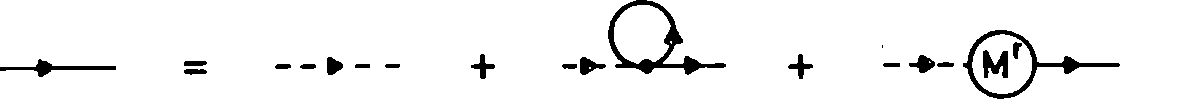
\includegraphics[width=0.7\linewidth]{pictures/Feq38.png}}}\label{eq:F_38}
\end{equation}
其中
\begin{equation}
\vcenter{\hbox{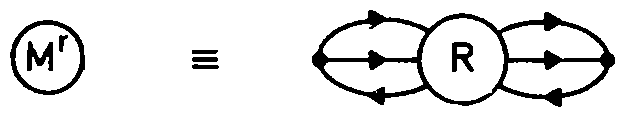
\includegraphics[width=0.4\linewidth]{pictures/Feq39.png}}}\label{eq:F_39}
\end{equation}
这里 $R$ 代表式 \ref{eq:F_25} 和式 \ref{eq:F_21} 中出现的Green函数的特殊组合。式 \ref{eq:F_38}
中的虚线代表式 \ref{eq:F_34} 的完全自由Green函数 $G^{00}$。

为了解析地推导微扰论（其优点在于特定项的系数因子与正负符号可以直接严密得出），我们从所谓的多时间 $n$ 体Green函数的定义出发：
\begin{align}
 & G(1,2,\dots,n;1',2',\dots,n')\nonumber \\
 & =(-\mathrm{i})^{n}\langle0|\mathcal{T}\{a(1)a(2)\dots a(n)a^{\dagger}(n')\dots a^{\dagger}(2')a^{\dagger}(1')\}|0\rangle\nonumber \\
 & =(-\mathrm{i})^{n}\sum_{\text{all permu-}}(-)^{P}\Big\{\Theta(t_{1}-t_{2})\Theta(t_{2}-t_{3})\dots\Theta(t_{n-1}-t_{n})\Theta(t_{n}-t_{n'})\Theta(t_{n'}-t_{(n-1)'})\dots\Theta(t_{2'}-t_{1'})\nonumber \\
 & \quad\cdot\langle0|a(1)a(2)\dots a(n)a^{\dagger}(n')\dots a^{\dagger}(1')|0\rangle\Big\}.\label{eq:F_40}
\end{align}
定义 \ref{eq:F_40} 意味着算符始终按照其时间参数从右到左递增的方式进行编时排列。也很容易看出，表达式 \ref{eq:F_40}
关于任意两个指标的对换是完全反对称的。我们想要写出Green函数 \ref{eq:F_40} 的运动方程，这对于单体和两体情形很容易证明；然而对于一般情况，证明过程相当繁琐，我们建议感兴趣的读者参考标准文献
\cite{Mi67,AGD65}：
\begin{align}
 & G^{00-1}(1,1'')\cdot G(1'',2\dots n;1'\dots n')\nonumber \\
 & =\sum^{n}_{l=1}(-)^{l+1}\delta(1,l')\cdot G(2\dots n;1'\dots l'-1,l'+1,\dots n')\nonumber \\
 & \quad-\frac{\mathrm{i}}{2}\bar{v}(1,n'+1;1'',n+1)\cdot G(1'',2\dots n,(n+1)^{+};1'\dots n',(n'+1)^{++}).\label{eq:F_41}
\end{align}
参数上的正号表示相应的时间参数移位了一个正的无穷小量，即 $1^{+}=p_{1},t_{1}+0$ 以及 $1^{++}=p_{1},t_{1}+0+0$。两体相互作用矩阵元由下式给出：
\begin{equation}
\bar{v}(1,2;3,4)=\delta(t_{1}-t_{2})\delta(t_{3}-t_{4})\delta(t_{1}-t_{3})\bar{v}_{1234}.\label{eq:F_42}
\end{equation}

求逆运动方程 \ref{eq:F_41} 是非常有用的：
\begin{align}
 & G(1\dots n;1'\dots n')\nonumber \\
 & =\sum^{n}_{l=1}(-)^{l+1}G^{00}(1,l')G(2\dots n;1'\dots l'-1,l'+1\dots n')\nonumber \\
 & \quad-\frac{\mathrm{i}}{2}G^{00}(1,1''')\bar{v}(1''',n'+1;1'',n+1)\cdot G(1'',2\dots n,(n+1)^{+};1'\dots n',(n'+1)^{++}).\label{eq:F_43a}
\end{align}
其伴随方程的形式为：
\begin{align}
 & G(1\dots n;1'\dots n')\nonumber \\
 & =\sum^{n}_{l=1}(-)^{l+1}G(1\dots l-1,l+1\dots n;2'\dots n')G^{00}(l,1')\nonumber \\
 & \quad-\frac{\mathrm{i}}{2}G(1\dots n,(n+1)^{++};1'',2'\dots n',(n'+1)^{+})\bar{v}(n'+1,1'';n+1,1''')G^{00}(1''',1').\label{eq:F_43b}
\end{align}
我们看到，运动方程将 $n$ 体Green函数与 $(n\pm1)$ 体Green函数联系了起来。从式 \ref{eq:F_43a}
中，我们很容易推导出完全忽略两体相互作用的近似下 $n$ 体Green函数的表达式 $G^{00}(1\dots n;1'\dots n')$：
\begin{equation}
G^{00}(1\dots n;1'\dots n')=\det|G^{00}(i,j)|.\label{eq:F_44}
\end{equation}

由此，如何计算 $n$ 体Green函数的一阶表达式就十分清楚了：我们首先利用两体Green函数的式 \ref{eq:F_44}
计算单体Green函数的一阶贡献。两体Green函数耦合到单体和三体Green函数。单体Green函数的一阶由前一步已知，而三体Green函数可通过式
\ref{eq:F_44} 计算到零阶；这便得出了两体Green函数的一阶贡献。我们可以按此方案继续推演，以计算 $n$ 体Green函数的一阶。为了计算二阶，我们需要一阶表达式，由此建立起类似的递推方案。这一过程随后可以重复进行到任意阶。

\section{骨架展开}

对于许多问题，我们并不太关心用 $G^{00}(1,1')$ 表示的展开项，而是希望得到按精确 $G(1,1')$ 的幂次展开（骨架展开，skeleton
expansion）。微扰级数的这种部分重求和之所以可能，可以通过仅涉及 $G^{00}(1,1')$ 的级数研究来证明。我们可以通过将式
\ref{eq:F_43a} 从左侧乘以式 \ref{eq:F_19b} 并利用式 (F.9, 12) 来推导骨架展开：
\begin{align}
 & G(1\dots n;1'\dots n')\nonumber \\
 & =\sum^{n}_{l=1}(-)^{l+1}G(1,l')\cdot G(2\dots n;1'\dots l'-1,l'+1\dots n')\nonumber \\
 & \quad-\frac{\mathrm{i}}{2}G(1,1''')\bar{v}(1''',n'+1;1'',n+1)\cdot R(1'',2\dots n,(n+1)^{+};1'\dots n',(n'+1)^{++}),\label{eq:F_45}
\end{align}
其中
\begin{align}
 & R(1\dots n,n+1;1'\dots n',n'+1)\nonumber \\
 & =G(1\dots n,n+1;1'\dots n',n'+1)-G(1,n+1;1'',n'+1)G^{-1}(1'',2'')G(2'',2\dots n;1'\dots n').\label{eq:F_46}
\end{align}
与按 $G^{00}(1,1')$ 幂次展开的情形一样，我们从式 \ref{eq:F_45} 中看出，对于骨架展开，零阶骨架贡献由下式给出：
\begin{equation}
G^{\text{skeleton}}(1\dots n;1'\dots n')\equiv G^{0}(1\dots n;1'\dots n')=\det|G(i,j)|,\label{eq:F_47}
\end{equation}
也就是说，在最低阶骨架近似下，$n$ 体Green函数就是相应单体Green函数的反对称化积。现在基本上按完全自由情形相同的方式推进，我们从式
(F.45, 46, 47) 即可获得骨架展开的连续各阶项。应当注意，式 \ref{eq:F_46} 的最低阶已不再是反对称化积，式
\ref{eq:F_46} 右侧的第二项恰好从第一项中扣除了在式 \ref{eq:F_45} 右侧第一项最低阶中已经重求和过的部分。读者不妨选取一个具体示例亲自验证这一事实。

上述推导骨架展开的规程是清晰明了的，它能自动给出给定阶项的正确符号和前置因子。视具体示例和展开阶数而定，其推导可能相当冗长。为了经济高效地进行这些计算，实际演算练习是必不可少的，这也是所有微扰展开技术的共同特征。为了更熟悉这些步骤，我们建议读者验证以下事实：质量算符动态部分的表达式
\ref{eq:F_25} 包含一个广义三体Green函数 \cite{ES69}：
\begin{equation}
R(1,2,3;1',2',3')=G(1,2,3;1',2',3')-G(1,2;1'',2')G^{-1}(1'',1''')G(1''',3;1',3').\label{eq:F_48}
\end{equation}
验证式 \ref{eq:F_48} 右侧的第一项和第二项（在二阶上）都包含具有图 \ref{fig:F_1} 所示结构的项，且它们恰好相互抵消。人们通常称质量算符的动态部分是单线不可约的（one-line
irreducible），即它不包含仅通过切断一条费米子线就能被分割成两部分的图。进一步的考察表明，式 \ref{eq:F_48}
第二项的所有图都是单线可约的，且这些项精确抵消了式 \ref{eq:F_48} 第一项中所包含的相等项。余下的部分则是不可约的。

\begin{figure}[H]
\begin{centering}
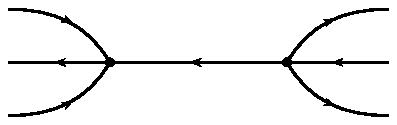
\includegraphics[width=0.4\linewidth]{pictures/F_1}
\par\end{centering}
\caption{\label{fig:F_1}式 (F.48) 中两项的二阶贡献。}
\end{figure}

质量算符的二阶骨架展开可以很容易地从式 \ref{eq:F_48} 结合式 \ref{eq:F_47} 计算得出：
\begin{equation}
M^{(2)}(1,1')=\frac{1}{2}\bar{v}(1,2';1''',2)G(1''',1'')G(2,3')G(3,2')\bar{v}(3',1'';3,1'),\label{eq:F_49}
\end{equation}
其图形表示示于图 \ref{fig:F_2}。在图 \ref{fig:F_3} 中，我们非常示意性地给出了式 \ref{eq:F_48}
中所包含的一些更高阶项。在示意绘图中，我们没有画出交换图。

\begin{figure}[H]
\begin{centering}
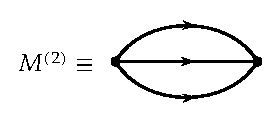
\includegraphics[width=0.35\textwidth]{pictures/F_2}
\par\end{centering}
\caption{\label{fig:F_2}质量算符二阶骨架贡献的图形表示。}
\end{figure}

\begin{figure}[H]
\begin{centering}
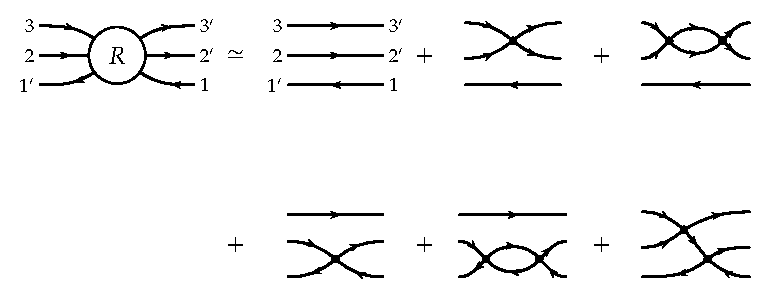
\includegraphics[width=0.75\textwidth]{pictures/F_3}
\par\end{centering}
\caption{\label{fig:F_3}质量算符中所含Green函数的更高阶贡献项。}
\end{figure}


\section{因子化与Brueckner-Hartree-Fock理论}

$n$ 体Green函数的一个重要特征在于它们能够近似因子化为更低阶Green函数的反对称化积。这一点可以通过对相应微扰级数的广泛研究来加以验证。例如在图
\ref{fig:F_3} 中我们看到，前五个图项恰好是如下因子化展开的开端：
\begin{align}
R(1,2,3;1',2',3') & \simeq G(1,1')\cdot G(2,3;2',3')\nonumber \\
 & \quad+\Big\{\left[G(2,2')\cdot R(1,3;1',3')-(3\leftrightarrow2)\right]-\left[3'\leftrightarrow2'\right]\Big\}\nonumber \\
 & \quad+\Big\{\left[G(2,2')\cdot G(1,1')\cdot G(3,3')-(3\leftrightarrow2)\right]-\left[3'\leftrightarrow2'\right]\Big\},\label{eq:F_50}
\end{align}
其中
\begin{equation}
R(1,3;1',3')=G(1,3;1',3')+G(1,3')\cdot G(3,1').\label{eq:F_51}
\end{equation}
函数 \ref{eq:F_51} 本质上等价于式 (8.130) 中定义的线性响应函数\footnote{式 (8.130) 中定义的响应函数在时间坐标空间中对 $t_{1}=t_{1'}$ 和 $t_{3}=t_{3'}$ 由 $-\mathrm{i}\Theta(t_{1}-t_{3})\langle0|[a^{\dagger}(1')a(1),a^{\dagger}(3')a(3)]|0\rangle$
给出。该定义与式 (F.51) 的区别在于式 (8.130) 第二项中 $\mathrm{i}\eta$ 的符号、一个额外的因子
$(-\mathrm{i})$ 以及费米子算符的排列顺序。由于两种定义的物理内容完全相同，我们可以在两种形式下自由切换工作。}；通过将式 \ref{eq:F_51} 与式 (8.131) 进行比对，可以证实我们必须加上式 \ref{eq:F_51} 中的第二项。

初学者容易感到困惑的一个特点是：因子化式 \ref{eq:F_50}——即除单粒子Green函数的三重积之外的所有项——并没有给出式
\ref{eq:F_48} 的正确最低阶骨架项，亦即它未能直接重现表达式 \ref{eq:F_49}。因子化仅对关联部分有效，亦即对式
\ref{eq:F_48} 中所包含的二阶、三阶、四阶、五阶以及所有相应的更高阶图（图 \ref{fig:F_3}）有效。为了修正并配平出正确的最低阶贡献，我们在式
\ref{eq:F_50} 的因子化中必须补加上 $G(i,j)$ 的三重积。另一方面，关联部分求和了式 \ref{eq:F_50}
中出现的精确两体关联函数中所包含的无穷子级数，因此因子化可以构成一种非常强大的近似方案。

我们注意到，式 \ref{eq:F_50} 右侧的第一项求和了粒子-粒子（pp）关联（见图 \ref{fig:F_3}），正如我们在4.3节中所讨论的，这些关联对于处理由裸核子-核子力硬芯所引入的短程关联至关重要。因此，若我们只想处理这些关联，便可以舍去式
\ref{eq:F_50} 中的其他项，并将质量算符写为：
\begin{equation}
M(1,1')=T(1,2;1',4)G(4,2)\label{eq:F_52}
\end{equation}
其中 $T$ 矩阵由下式给出：
\begin{equation}
T(1,2;1',4)=\bar{v}(1,2;1',4)+\frac{1}{4}\bar{v}(1,2;3',4')G(3',4';5,6)\bar{v}(5,6;1',4).\label{eq:F_53}
\end{equation}
对于式 \ref{eq:F_53} 中出现的两体Green函数，存在一个著名的积分方程（见下文）\cite{Mi67}：
\begin{equation}
G(1,2;1',2')=G^{0}(1,2;1',2')-\frac{1}{4}G^{0}(1,2;3,4)K^{pp}(3,4;3',4')G(3',4';1',2'),\label{eq:F_54}
\end{equation}
其中 $K^{pp}$ 是一种有效 pp 力，在最低阶下由下式给出：
\begin{equation}
K^{pp}(3,4;3',4')\simeq\bar{v}(3,4;3',4').\label{eq:F_55}
\end{equation}

如果我们进而利用式 (F.28, 29) 将式 \ref{eq:F_54} 中的单粒子Green函数替换为其HF表达式，并在式 (F.28,
29) 中略去第二部分（空穴贡献；可以证明空穴线在密度展开中属于更高阶，因此被认为显著小于粒子贡献；参见例如 \cite{Ma67b}），结合式
(F.52-55)，我们便求得了Brueckner-Hartree-Fock方程 (5.72) 的结构。我们现在必须认识到，$T$
矩阵 \ref{eq:F_53} 实际上仅依赖于一个时间差，在Fourier变换后引起能量依赖性。如果这一能量依赖性按照式 (5.75)
的规则加以替换，我们就可以将式 \ref{eq:F_52} 和式 \ref{eq:F_53} 与Brueckner-HF方程 (5.72)
严格完全等同起来。

\section{Hartree-Fock-Bogoliubov方程}

不仅推导Brueckner-Hartree-Fock理论非常有益，利用Green函数技术推导Hartree-Fock-Bogoliubov（HFB）理论同样富有启发性。为此，我们再次仅保留式
\ref{eq:F_50} 右侧的第一项，因为我们已经知道配对关联属于 pp 关联。式 \ref{eq:F_50} 第一项中的空穴Green函数
$G(1,1')$ 是仅使用质量算符的静态部分计算的。对于两体Green函数，我们需要给出其谱表示：
\begin{align}
G_{12,1'2'}(t-t') & =(-\mathrm{i})^{2}\langle0|\mathcal{T}\{a_{1}(t)a_{2}(t)a^{\dagger}_{2'}(t')a^{\dagger}_{1'}(t')\}|0\rangle\nonumber \\
 & =(-\mathrm{i})^{2}\Big\{\Theta(t-t')\sum_{\rho^{+}}\langle0|a_{1}a_{2}|\rho^{+}\rangle\langle\rho^{+}|a^{\dagger}_{2'}a^{\dagger}_{1'}|0\rangle\mathrm{e}^{-(\mathrm{i}/\hbar)(E^{A+2}_{\rho}-E^{A}_{0})(t-t')}\nonumber \\
 & \quad+\Theta(t'-t)\sum_{\rho^{-}}\langle0|a^{\dagger}_{2'}a^{\dagger}_{1'}|\rho^{-}\rangle\langle\rho^{-}|a_{1}a_{2}|0\rangle\mathrm{e}^{-(\mathrm{i}/\hbar)(E^{A}_{0}-E^{A-2}_{\rho})(t-t')}\Big\}\label{eq:F_56}
\end{align}
或者在Fourier变换之后：
\begin{equation}
G_{12,1'2'}(\omega)=(-\mathrm{i})\left\{ \sum_{\rho^{+}}\frac{\langle0|a_{1}a_{2}|\rho^{+}\rangle\langle\rho^{+}|a^{\dagger}_{2'}a^{\dagger}_{1'}|0\rangle}{\omega-\Omega^{pp}_{\rho}+\mathrm{i}\eta}-\sum_{\rho^{-}}\frac{\langle0|a^{\dagger}_{2'}a^{\dagger}_{1'}|\rho^{-}\rangle\langle\rho^{-}|a_{1}a_{2}|0\rangle}{\omega-\Omega^{hh}_{\rho}-\mathrm{i}\eta}\right\} ,\label{eq:F_57}
\end{equation}
其中 $E^{A\pm2}_{\rho},E^{A}_{0}$ 是精确本征能量，且
\[
\hbar\Omega^{pp}_{\rho}=E^{A+2}_{\rho}-E^{A}_{0},\quad\hbar\Omega^{hh}_{\rho}=E^{A}_{0}-E^{A-2}_{\rho}.
\]

HFB理论隐含地假定在式 \ref{eq:F_57} 的 $\rho$ 求和中只有基态是起主导作用的，也就是说，它们被假定具有高度的集体性，以至于在式
\ref{eq:F_57} 的留数求和（它是一个常数）中，基态的留数汇集了几乎全部的强度。正如我们在第11章中所阐述的，特定模式的集体性概念是相变（在此即向超流态的相变）的核心本质特征。

牢记式 \ref{eq:F_50} 第一项中的单粒子Green函数在质量算符中演化为空穴线，利用式 (F.21)、式 (F.22)
和式 \ref{eq:F_50}，我们在质量算符的动态部分中分离出所谓的Cooper极点 \cite{Pi61}\footnote{我们应当注意到，对于空穴线，Dyson方程的方向是反转的，因此在式 (F.58) 中出现的是单粒子势的复共轭。这也可以在微扰论中针对式
(F.39) 中的 $R$ 函数加以验证。然而，这一点仅在单粒子Hamilton量不具备时间反演不变性时才具有实际意义。}，从而获得如下近似Dyson方程 {[}推导时应完全在时间坐标空间中利用式 (F.29) 进行，仅在最后一步执行Fourier变换{]}：
\begin{align}
(\hbar\omega-\varepsilon_{1})G_{11'}(\omega) & =\delta_{11'}+\bar{v}_{1234}\rho_{42}G_{31'}(\omega)+M^{\text{Cooper}}_{12}\cdot G_{21'}(\omega),\nonumber \\
M^{\text{Cooper}}_{11'}(\omega) & =\Delta^{(+)}_{12}\cdot\left(\frac{\rho}{\hbar\omega-\hbar\Omega^{pp}_{0}+h^{*}}\right)_{22'}\cdot\Delta^{(+)*}_{2'1'}\nonumber \\
 & \quad+\Delta^{(-)}_{12}\cdot\left(\frac{1-\rho}{\hbar\omega-\hbar\Omega^{hh}_{0}+h^{*}}\right)_{22'}\cdot\Delta^{(-)*}_{2'1'},\label{eq:F_58}
\end{align}
其中
\begin{align}
\Delta^{(+)}_{12} & =-\frac{1}{2}\bar{v}_{1234}\langle0|a_{3}a_{4}|A+2,0\rangle,\nonumber \\
\Delta^{(-)}_{12} & =-\frac{1}{2}\bar{v}_{1234}\langle A-2,0|a_{3}a_{4}|0\rangle.\label{eq:F_59}
\end{align}
因为我们只考虑束缚态问题，所以可以忽略式 \ref{eq:F_58} 分母中的无穷小量 $\pm\mathrm{i}\eta$。针对向超流态相变的情况，我们可以作出的下一个近似是：
\begin{align}
\hbar\Omega^{pp}_{0} & \simeq2(E^{A+1}_{0}-E^{A}_{0})=2\lambda^{(+)},\nonumber \\
\hbar\Omega^{hh}_{0} & \simeq2(E^{A}_{0}-E^{A-1}_{0})=2\lambda^{(-)}.\label{eq:F_60}
\end{align}
这一近似意味着构成Cooper对的两个粒子的关联能为零。这当然是我们在处理相变时可以作出的另一个假设：特定激发模变得如此之软，以致其激发能趋近于零。最后，我们假定对于大系统可以进一步作出粒子数不守恒近似（该近似也可以避免
\cite[1.4.6节]{Mi67}）：
\begin{equation}
\Delta^{(+)}\simeq\Delta^{(-)}=\Delta;\quad\lambda^{(+)}\simeq\lambda^{(-)}=\lambda.\label{eq:F_61}
\end{equation}
由此我们便导出了著名的Gorkov方程 \cite{Go58}：
\begin{align*}
(\hbar\omega'-h')_{12}G_{21'} & =\hbar\delta_{11'}-\Delta_{12}F^{*}_{21'},\\
(\hbar\omega'+h'^{*})_{12}F^{*}_{21'} & =\Delta^{*}_{12}G_{21'},
\end{align*}
或写成矩阵形式：
\begin{equation}
\begin{pmatrix}\hbar\omega' & 0\\
0 & \hbar\omega'
\end{pmatrix}_{12}\begin{pmatrix}G\\
-F^{*}
\end{pmatrix}_{21'}=\begin{pmatrix}\hbar\delta_{11'}\\
0
\end{pmatrix}+\begin{pmatrix}h' & \Delta\\
-\Delta^{*} & -h'^{*}
\end{pmatrix}_{12}\begin{pmatrix}G\\
-F^{*}
\end{pmatrix}_{21'},\label{eq:F_62}
\end{equation}
其中我们引入了记号 $\hbar\omega'=\hbar\omega-\lambda,h'=h-\lambda$，且
\begin{equation}
F^{*}_{11'}=-\left(\frac{1}{\hbar\omega'+h'^{*}}\right)_{12}\Delta^{*}_{22'}G_{2'1'}.\label{eq:F_63}
\end{equation}

在式 \ref{eq:F_62} 的右侧，我们认出了式 (7.39) 中熟悉的HFB矩阵 $\mathcal{H}$。照例，我们可以写出
$G(1,1')$ 的谱表示 (F.6a, b)，并且从式 \ref{eq:F_63} 中看出对于 $F^{*}(1,1')$
同样可以建立谱表示：
\begin{align}
G_{11'}(\omega) & =\hbar\sum_{k}\frac{V^{*}_{1k}V_{1'k}}{\hbar\omega+E_{k}-\mathrm{i}\eta}+\frac{U_{1k}U^{*}_{1'k}}{\hbar\omega-E_{k}+\mathrm{i}\eta},\nonumber \\
-F^{*}_{11'}(\omega) & =\hbar\sum_{k}\frac{U^{*}_{1k}V_{1'k}}{\hbar\omega+E_{k}-\mathrm{i}\eta}+\frac{V_{1k}U^{*}_{1'k}}{\hbar\omega-E_{k}+\mathrm{i}\eta}.\label{eq:F_64}
\end{align}
从式 \ref{eq:F_64} 中我们发现，在极点处方程 \ref{eq:F_62} 与HFB方程 (7.42) 完全等同。

为了闭合该方程组，我们必须阐明如何从解 $G_{11'},F^{*}_{11'}$ 中求得配对能隙 $\Delta$。为此，我们将式
\ref{eq:F_59} 中出现的跃迁振幅表述为：
\begin{equation}
\langle0|a_{3}a_{4}|A+2,0\rangle=\lim_{\substack{t=t_{2}=t_{1}+0\rightarrow-\infty\\
t_{3}=t_{4}+0\rightarrow0
}
}\exp(-\mathrm{i}\Omega^{pp}_{0}t)\frac{\langle0|\mathcal{T}\{a(3)a(4)a^{\dagger}(2)a^{\dagger}(1)\}|0\rangle}{\langle A+2,0|a^{\dagger}_{2}a^{\dagger}_{1}|0\rangle}.\label{eq:F_65}
\end{equation}
该关系式 \cite{WE70} 可以通过从时间极限过渡到Abel极限来证明其成立：
\begin{align}
|A+2,0\rangle & =\lim_{\eta\rightarrow0}\eta\int^{0}_{-\infty}\mathrm{d}t\,\mathrm{e}^{\eta t}\frac{\mathrm{e}^{-\mathrm{i}\Omega^{pp}_{0}t}}{\langle A+2,0|a^{\dagger}_{2}a^{\dagger}_{1}|0\rangle}a^{\dagger}_{2}(t)a^{\dagger}_{1}(t)|0\rangle\nonumber \\
 & =\lim_{\eta\rightarrow0}\frac{\eta}{\langle A+2,0|a^{\dagger}_{2}a^{\dagger}_{1}|0\rangle}\sum_{\tau}\frac{\langle A+2,\tau|a^{\dagger}_{2}a^{\dagger}_{1}|0\rangle}{-\mathrm{i}(E^{A+2}_{0}-E^{A+2}_{\tau}+\mathrm{i}\eta)}|A+2,\tau\rangle\nonumber \\
 & =|A+2,0\rangle.\quad\text{证毕（Q.E.D.）}\label{eq:F_66}
\end{align}
对于式 \ref{eq:F_65} 中出现的两体Green函数，我们可以利用积分方程 \ref{eq:F_54}；将 $K^{pp}$
前面的单粒子Green函数之一替换为其最低阶表达式 \ref{eq:F_26}，并将具有式 \ref{eq:F_55} 的式 \ref{eq:F_54}
代入式 \ref{eq:F_65} 中，结合式 \ref{eq:F_61} 和式 \ref{eq:F_63}，我们便得到了“能隙方程”：
\begin{equation}
\Delta_{12}=\frac{1}{2}\bar{v}_{1234}\frac{1}{2\pi\mathrm{i}}\oint\mathrm{d}\omega\,F_{34}(\omega).\label{eq:F_67}
\end{equation}
因此，结合式 \ref{eq:F_62}，我们获得了完全闭合的自洽方程组。我们在式 \ref{eq:F_54} 中将其中一个单粒子Green函数替换为其最低阶表达式
\ref{eq:F_26}，表面上看起来似乎是对式 \ref{eq:F_54} 中两个单粒子Green函数的非对称处理；然而，正如Gorkov方程
\ref{eq:F_62} 的推导所表明的，这与质量算符的近似 \ref{eq:F_58} 是完全内在自洽的。

我们想对刚刚推导出的这组耦合方程给出图形化与物理学解释。方程 \ref{eq:F_58} 在图 \ref{fig:F_4}a 中给出图形表示，而方程
\ref{eq:F_67} 则在图 \ref{fig:F_4}b 中表示。

\begin{figure}[H]
\begin{centering}
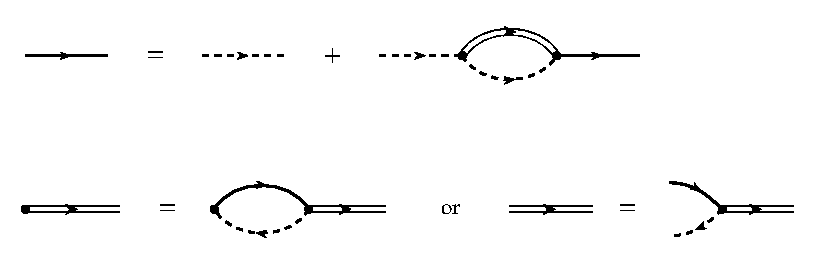
\includegraphics[width=0.7\textwidth]{pictures/F_4}
\par\end{centering}
\caption{\label{fig:F_4}(a) 式 (F.58) 的图形表示，其中虚线代表最低阶近似 (F.26)，双线代表配对模。(b)
能隙方程 (F.67) 的图形表示。}
\end{figure}

从图 \ref{fig:F_4} 中我们可以看出，用Green函数的语言来表达，HFB方程的物理内涵在于：配对模是由单粒子传播子计算得出的，而这些传播子本身又通过粒子与配对模及空穴的耦合而发生重整化。这些耦合方程的求解隐含地求和了微扰级数的一个重要组成部分，从而允许我们描述宏观相变。

在推导Brueckner-HF理论和HFB理论时，我们最初对质量算符采用了相同的近似形式 {[}式 \ref{eq:F_50} 右侧的第一项{]}，这可能会让人感到困惑。然而应当认识到，Brueckner-HF理论从未分离出式
\ref{eq:F_50} 两体Green函数中所包含的Cooper极点。我们在HFB理论中显式地处理这一极点，因此与Brueckner-HF并不冲突；我们也可以在统一的Brueckner-HFB理论框架下将这两种理论结合起来。

到目前为止，我们讨论了从正常态到超流态的相变，并展示了某一个特定的 pp 模如何汇集几乎全部集体性，并随之变得非常软，从而使我们能够导出HFB方程。从我们早先的考察（参见第7章）可知，HFB方程允许球形解（保持空间转动对称性）和形变解（破缺空间转动对称性）。然而在我们对配对现象的处理中，我们未曾在任何地方假设过转动对称性的破缺——我们始终假定
$\rho_{11'}=\langle0|a^{\dagger}_{1'}a_{1}|0\rangle$ 对应于具有良好角动量的基态密度（为了明确思路，例如对偶偶核取
$I=0$）。从第7章和第11章关于从球形核向形变核相变的论述中，我们知道这恰好与另一种软模——四极振动相关联。我们将更详细地展示这在Green函数形式体系中是如何描述的。

显而易见，为了处理从球形态向形变态的转变，我们必须在质量算符 \ref{eq:F_25} 中分离出粒子与四极声子的耦合。这可以通过仅从因子化式
\ref{eq:F_50} 中保留出现响应函数 \ref{eq:F_51} 的那些项来最容易地实现。谱分解随后给出了 $A$
体系统的激发能 (8.130)：
\begin{equation}
R_{13,1'3'}(\omega)=\mathrm{i}\sum_{\mu>0}\left(\frac{\langle0|a^{\dagger}_{1'}a_{3'}|\mu\rangle\langle\mu|a^{\dagger}_{3}a_{1}|0\rangle}{\omega-\Omega^{ph}_{\mu}+\mathrm{i}\eta}-\frac{\langle0|a^{\dagger}_{3}a_{1}|\mu\rangle\langle\mu|a^{\dagger}_{1'}a_{3'}|0\rangle}{\omega+\Omega^{ph}_{\mu}-\mathrm{i}\eta}\right).\label{eq:F_68}
\end{equation}
如同处理配对模的情形一样，我们现在假定式 \ref{eq:F_68} 中最低的激发几乎耗尽了全部的跃迁强度，并且其激发能趋近于零（$\Omega^{ph}_{\mu}\rightarrow0$）。在此我们假定四极模通常具有这种性质（确实，对于转动核，其激发能变得非常低）；然而，有时其他激发模也可能成为最低的激发态（例如在
$^{208}\text{Pb}$ 中）。对于式 \ref{eq:F_50} 中出现的单粒子Green函数，我们再次采用最低阶近似
\ref{eq:F_26}。Dyson方程于是具有如下形式：
\begin{align}
(\hbar\omega-\varepsilon_{1})G_{11'}(\omega) & =\delta_{11'}+\bar{v}_{1234}\rho_{42}G_{31'}(\omega)+M^{\text{phonon}}_{12}G_{21'}(\omega),\label{eq:F_69}
\end{align}
其中
\begin{equation}
M^{\text{phonon}}_{11'}(\omega)=Q^{\overbracket{2^{+}2}}_{1}\left(\frac{1}{\hbar\omega-h}\right)_{22'}Q^{\overbracket{2^{+}2'}*}_{1'},\label{eq:F_70}
\end{equation}
以及
\begin{equation}
Q^{\overbracket{2^{+}2}}_{1}=\bar{v}_{1(324)_{j_{1}}}\langle0|[a^{\dagger}_{3}a_{4}]_{2^{+}}|2^{+}\rangle.\label{eq:F_71}
\end{equation}

应当指出，到目前为止我们尚未作出任何破缺对称性的近似，因为——正如符号所指明的——所有量都已耦合到良好角动量（我们将粒子 2 或 $2'$
与四极声子耦合以给出外场粒子的角动量 $j_{1}$）。我们还应当认识到，式 \ref{eq:F_71} 中的 $Q$ 场对应于9.3.3节中粒子-振动耦合理论的
$\gamma$ 顶点（不含因子 $\frac{1}{2}$；见第386页脚注讨论）。通过引入如下量：
\begin{equation}
P_{11'}=-\left(\frac{1}{\hbar\omega-h}\right)_{12}Q^{\overbracket{2^{+}2}*}_{2'}G_{2'1'},\label{eq:F_72}
\end{equation}
我们可以再次将式 (F.69, 70) 改写为两个相互耦合的方程形式：
\begin{align}
(\hbar\omega-h)_{12}G_{21'}(\omega) & =\delta_{11'}+Q^{\overbracket{2^{+}2}}_{1}P^{*}_{21'}(\omega),\nonumber \\
(\hbar\omega-h)_{12}P^{*}_{21'}(\omega) & =-Q^{\overbracket{2^{+}1}*}_{2}G_{21'}(\omega).\label{eq:F_73}
\end{align}
如同配对的情形一样，我们必须使方程组闭合。在此可以通过使用响应函数的Bethe-Salpeter方程 (8.131) 来代替式 \ref{eq:F_50}，从而以完全类似的方式达成这一目标。其结果为：
\begin{equation}
\langle0|[a^{\dagger}_{3}a_{4}]_{2^{+}}|2^{+}\rangle=\delta\rho^{(2^{+})}_{43}=\frac{1}{2\pi\mathrm{i}}\oint\mathrm{d}\omega\,P_{43}(\omega).\label{eq:F_74}
\end{equation}
将式 \ref{eq:F_74} 代入式 \ref{eq:F_71} 中，连同式 \ref{eq:F_73} 一起，便构成了形变场“序参量”
$Q$ 的“能隙方程”。

两个单粒子场进入方程组 (F.73)，一个涉及普通密度 $\rho_{12}=\langle0|a^{\dagger}_{2}a_{1}|0\rangle$，另一个涉及跃迁密度
\[
\delta\rho^{(2^{+})}_{12}=\langle0|[a^{\dagger}_{2}a_{1}]_{2^{+}}|2^{+}\rangle.
\]
跃迁密度自然投影出了式 \ref{eq:F_71} 中 $ph$ 力的四极部分，而普通密度则投影出了式 \ref{eq:F_69}
中力的单极部分。我们再次强调：到目前为止没有作出任何破坏对称性的近似，因为我们已经把所有量都耦合到了良好的角动量。形变HF理论的对称性破缺可以通过将
$2^{+}$ 态等同于内禀系统的基态而引入。在此时，进行角动量耦合便不再有意义，方程 \ref{eq:F_73} 随即退化为通常的形变HF方程。我们显式地求出了在11.2节中引入的两个势
$V_{0}$ 与 $\Gamma_{2}$，它们现在构成了内禀系统的非角动量守恒单粒子Hamilton量。

正如我们已经指出的，形变场的“能隙方程” (F.71, 74) 同样可以从响应函数的Bethe-Salpeter方程 (8.131)
导出。然而从式 \ref{eq:F_74} 和式 \ref{eq:F_72} 可以看出，它可以图形化地表示为图 \ref{fig:F_5}b
所示的形式。方程 \ref{eq:F_69} 则表示在图 \ref{fig:F_5}a 中。图 \ref{fig:F_5}a,
b 再次清晰地揭示了单粒子运动与集体振动的典型非线性耦合。

\begin{figure}[H]
\begin{centering}
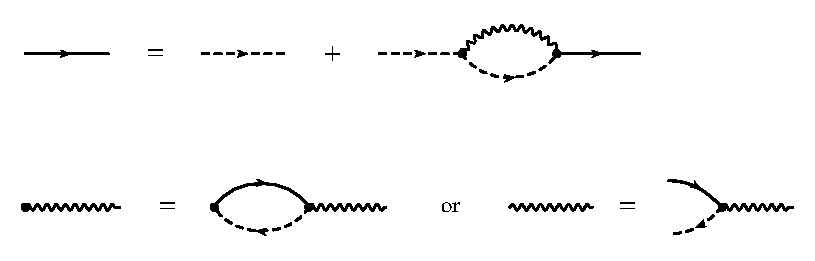
\includegraphics[width=0.7\textwidth]{pictures/F_5}
\par\end{centering}
\caption{\label{fig:F_5}(a) 方程 (F.69) 的图形表示，波浪线代表软四极声子。(b) 形变场 \$Q\$ 的“能隙方程”图形表示。}
\end{figure}

一般而言，我们当然应当在质量算符中同时分离出Cooper极点以及所有多极性的声子极点，从而生成我们在第7章中讨论的一般单粒子理论。从式
\ref{eq:F_71} 和式 \ref{eq:F_59} 中我们看到，跃迁密度进入了形变场和配对场。由于我们已经看到这些密度在核表面处达到峰值（第8章与第13章），因此将进入式
\ref{eq:F_71} 和式 \ref{eq:F_59} 的力替换为可分离力可能是一种极佳的近似。这自然导出了第7章讨论的配对加四极模型，因此我们在核相变的背景下再次领会了该模型的深刻意义。

从该理论的Green函数处理中，也可以清楚地看出一种可能的推广应如何运作：其核心特征在于将RPA模与单粒子态自洽地求解，也就是说，单粒子态以图
\ref{fig:F_5}a, b 所示的方式反作用耦合回到RPA模。此外，HFB理论的对称性守恒表述 \ref{eq:F_62}
应当是该理论的一个极具吸引力的变体；事实上，Janssen 已经提出了这种类型的一种更为精细的理论 \cite{Ja79}。

\section{Bethe-Salpeter方程与有效力}

在推导HFB方程的过程中，我们多次提到了针对两体Green函数的Bethe-Salpeter方程（BSE）。鉴于这些方程在许多教科书中均有详尽推导
\cite{Mi67,AGD65,FW71}，我们在此仅作极其简略的叙述。响应函数 \ref{eq:F_51} 的BSE由下式给出：
\begin{align}
R(1,3;1',3') & =G(1,1')G(3,3')\nonumber \\
 & \quad-G(3,5)G(6,1')K^{ph}(5,7;6,8)R(1,8;7,3').\label{eq:F_75}
\end{align}
方程 \ref{eq:F_75} 是一个精确方程，其中 $K^{ph}$ 被称为有效粒子-空穴力；它对响应函数中仅切断两条线无法被分割为两部分的骨架图进行了全求和。BSE
\ref{eq:F_75} 在图 \ref{fig:F_6} 中给出了图形表示，同时画出了对 $K^{ph}$ 的典型二阶贡献。我们看到，对
$K^{ph}$ 的这些贡献唯有切断四条线才能被分割成两半。方程 \ref{eq:F_75} 可以在骨架微扰展开的任意阶上加以验证。式
\ref{eq:F_75} 中的重复指标照例表示对量子数求和以及对时间积分。值得提及的是，式 \ref{eq:F_75} 在推导形式关系时有时非常方便。然而，超越RPA处理式
\ref{eq:F_75} 是极其复杂的，因为其积分核通常依赖于三个时间（在考虑了时间平移不变性之后）或三个能量。因此在实际应用中，我们有时使用核仅依赖于一个能量的响应函数积分方程
\cite{Sch71c,Sch76}。通过这种方式，我们得出了玻色子（RPA）的Dyson方程，其中包含玻色子质量算符，与费米子的Dyson方程
\ref{eq:F_22b} 非常类似 \cite{SE73,Sch76}。对关联函数的这种处理方式在精神上类似于在凝聚态领域中被称为Mori理论
\cite{Mo65} 的方法。在核物理中，该方法由 Werner 加以应用 \cite{We76,We78}。

\begin{figure}[H]
\begin{centering}
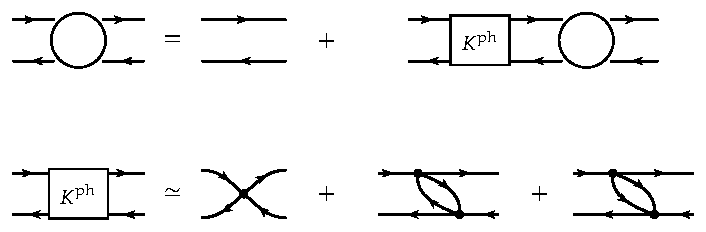
\includegraphics[width=0.7\textwidth]{pictures/F_6}
\par\end{centering}
\caption{\label{fig:F_6}响应函数 (F.50) 的Bethe-Salpeter方程及 \$K\textasciicircum\{ph\}\$
最低阶贡献的示意图。}
\end{figure}

我们关于响应函数的BSE所说的一切，对于两体Green函数的类似BSE \ref{eq:F_54} 同样完全成立：
\begin{align*}
G(1,2;1'2') & =G^{0}(1,2;1',2')-\frac{1}{4}G^{0}(1,2;3,4)K^{pp}(3,4;3',4')G(3',4';1',2').
\end{align*}
在此，$K^{pp}$ 再次求和了所有贡献于 $G(1,2;1',2')$ 且仅切断两条骨架线无法分为两半的图。在图 \ref{fig:F_7}
中，我们给出了式 \ref{eq:F_54} 的图形表示，以及对 $K^{pp}$ 的二阶骨架贡献；其最低阶自然就是裸相互作用本身。

\begin{figure}[H]
\begin{centering}
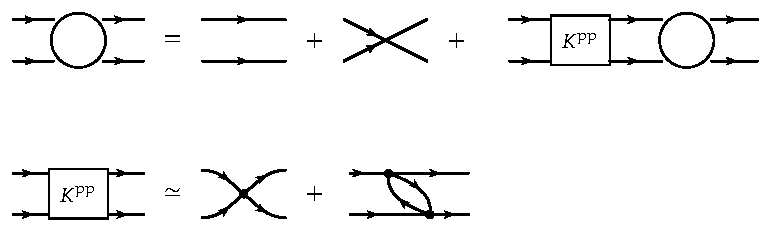
\includegraphics[width=0.75\textwidth]{pictures/F_7}
\par\end{centering}
\caption{\label{fig:F_7}式 (F.54) 的 \$pp\$ Green函数的Bethe-Salpeter方程及 \$K\textasciicircum\{pp\}\$
最低阶贡献的示意图。}
\end{figure}

正如我们在前文中所展示的，配对场 $\Delta$ 的能隙方程 \ref{eq:F_67} 和形变场 $Q$ 的能隙方程 \ref{eq:F_71}
可以分别从相应的Bethe-Salpeter方程 \ref{eq:F_54} 和 \ref{eq:F_75} 导出。因此显而易见，这些序参量必须分别使用相应的有效
$pp$ 力 $K^{pp}$ 和 $ph$ 力 $K^{ph}$ 进行计算。显式地证明这一点是相当精细的，给出全部细节会非常冗长，因此我们在此仅勾勒主要特征。

我们已经证明了在 $\Delta$ 和 $Q$ 的能隙方程中必须分别使用 $K^{pp}$ 和 $K^{ph}$。而要证明
$K^{pp}$ 和 $K^{ph}$ 分别如何在方程 \ref{eq:F_62} 和 \ref{eq:F_73} 的第一个方程中发挥作用则更为复杂。让我们将质量算符
\ref{eq:F_25} 中出现的 $R$ 函数记为 $R_{6}$；则对于质量算符，我们可以采用显而易见的简写记号写出：
\begin{equation}
M'(\omega)=\bar{v}R_{6}R^{-1}_{6}R_{6}\bar{v}.\label{eq:F_76}
\end{equation}
我们已经看到，HFB理论对应于将 $R_{6}$ 近似为式 \ref{eq:F_50} 右侧的第一项，我们将其记为 $GG_{4}$。在这一近似下，我们自然还有：
\begin{equation}
R^{-1}_{6}=[GG_{4}]^{-1}.\label{eq:F_77}
\end{equation}
我们现在注意到，从式 \ref{eq:F_45} 和式 \ref{eq:F_46} 我们有：
\begin{align}
G(1,2;1',2') & =G^{0}(1,2;1',2')\nonumber \\
 & \quad-\frac{\mathrm{i}}{2}R(1,2,3^{++};1'',2',3'^{+})\bar{v}(3',1'';3,1''')\cdot G(1''',1').\label{eq:F_78}
\end{align}
结合式 \ref{eq:F_54}，我们推导出恒等式：
\begin{align}
 & R(1,2,3^{++};1'',2',3'^{+})\bar{v}(3',1'';3,1''')\nonumber \\
 & =G(2,3^{++};2',3'^{+})\cdot G(1,1'')K^{pp}(3',1'';3,1''').\label{eq:F_79}
\end{align}
将式 \ref{eq:F_76} 中的部分 $R_{6}\bar{v}$ 和 $\bar{v}R_{6}$ 分别用式 \ref{eq:F_79}
及其伴随形式替换，并利用式 \ref{eq:F_77}，我们看出在式 \ref{eq:F_58} 和式 \ref{eq:F_62}
中我们必须处处使用 $K^{pp}$。类似地，我们当然也可以证明在式 \ref{eq:F_69} 和式 \ref{eq:F_73}
中必须处处使用 $K^{ph}$。可以证明 \cite{ES69}，我们通过近似 \ref{eq:F_77} 所忽略的项正是图
\ref{fig:F_8} 所示的类型，其中空穴从配对模发生散射。

\begin{figure}[H]
\begin{centering}
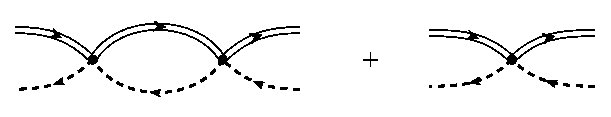
\includegraphics[width=0.5\textwidth]{pictures/F_8}
\par\end{centering}
\caption{\label{fig:F_8}式 (F.77) 近似中所略去的空穴-配对模散射过程。}
\end{figure}

至此我们结束对Green函数理论的简要概述，有关标准技术的更多细节，我们再次建议读者参阅本附录所引用的经典文献。


\bibliographystyle{alpha}
\nocite{*}
\bibliography{PeterRing}


\chapter*{专有术语英汉对照表}

\addcontentsline{toc}{chapter}{专有术语英汉对照表}
\markboth{专有术语英汉对照表}{专有术语英汉对照表}

本书翻译严格遵循统一的理论核物理中文学术术语体系。


\section*{1. 核心模型、方法与理论框架 (Core Theories \& Frameworks)}

\begin{longtable}{p{4.2cm} p{4.2cm} p{1.6cm} p{4.5cm}}
\toprule
\textbf{英文原名 (En)} & \textbf{规范中文译名 (Zh)} & \textbf{缩写/记号} & \textbf{重点说明 / 典型章节} \tabularnewline
\midrule
\endfirsthead
\toprule
\textbf{英文原名 (En)} & \textbf{规范中文译名 (Zh)} & \textbf{缩写/记号} & \textbf{重点说明 / 典型章节} \tabularnewline
\midrule
\endhead
\bottomrule
\endfoot
\bottomrule
\endlastfoot
Many-Body Problem & 多体问题 &  & 全书核心主题 \tabularnewline
Liquid Drop Model & 液滴模型 & LDM & 第 1 章 \tabularnewline
Shell Model & 壳模型 & SM & 第 2 章 \tabularnewline
Deformed Shell Model & 形变壳模型 &  & 第 2 章，Nilsson 势等 \tabularnewline
Mean Field Approximation & 平均场近似 &  & 贯穿全书 \tabularnewline
Self-Consistent Field & 自洽场 & SCF & 第 5、7 章 \tabularnewline
Hartree-Fock Method & Hartree-Fock 方法 / HF 方法 & HF & 第 5 章 \tabularnewline
Density-Dependent Hartree-Fock & 密度依赖的 Hartree-Fock 方法 & DDHF & 第 5 章，Skyrme / Gogny 力 \tabularnewline
Local Density Approximation & 局域密度近似 & LDA & 第 5、13 章 \tabularnewline
Pairing Correlation & 对关联 &  & 第 6 章 \tabularnewline
Superfluid Nuclei & 超流核 &  & 第 6 章 \tabularnewline
Seniority Model & 辛弱数模型 &  & 第 6 章，准自旋方法 \tabularnewline
BCS Theory & BCS 理论 & BCS & Bardeen-Cooper-Schrieffer 理论，第 6 章 \tabularnewline
Generalized Single-Particle Model & 推广的单粒子模型 &  & 第 7 章 \tabularnewline
Hartree-Fock-Bogoliubov Theory & Hartree-Fock-Bogoliubov 理论 & HFB & 第 7 章 \tabularnewline
Constrained Hartree-Fock / HFB & 约束 Hartree-Fock / 约束 HFB 理论 & CHF / CHFB & 第 7 章 \tabularnewline
Harmonic Vibrations & 简谐振动 &  & 第 8 章 \tabularnewline
Random Phase Approximation & 随机相位近似 & RPA & 第 8 章 \tabularnewline
Quasiparticle RPA & 准粒子随机相位近似 & QRPA & 第 8 章 \tabularnewline
Boson Expansion Method & 玻色展开方法 & BEM & 第 9 章 \tabularnewline
Generator Coordinate Method & 生成坐标法 & GCM & 第 10 章 \tabularnewline
Restoration of Broken Symmetries & 对称性的恢复 &  & 第 11 章 \tabularnewline
Spontaneous Symmetry Breaking & 自发对称性破缺 & SSB & 第 11 章 \tabularnewline
Projection Method & 投影方法 &  & 第 11 章，粒子数投影、角动量投影 \tabularnewline
Time-Dependent Hartree-Fock & 时间相关 Hartree-Fock 方法 & TDHF & 第 12 章 \tabularnewline
Semiclassical Methods & 半经典方法 &  & 第 13 章 \tabularnewline
\end{longtable}

\section*{2. 微观多体物理与算符代数 (Many-Body Physics \& Second Quantization)}

\begin{longtable}{p{4.8cm} p{4.8cm} p{5.0cm}}
\toprule
\textbf{英文原名 (En)} & \textbf{规范中文译名 (Zh)} & \textbf{常见符号 / 备注} \tabularnewline
\midrule
\endfirsthead
\toprule
\textbf{英文原名 (En)} & \textbf{规范中文译名 (Zh)} & \textbf{常见符号 / 备注} \tabularnewline
\midrule
\endhead
\bottomrule
\endfoot
\bottomrule
\endlastfoot
Second Quantization & 二次量子化 & 附录 C \tabularnewline
Creation Operator & 产生算符 & 粒子 $c_k^\dagger, a_k^\dagger$；准粒子 $\alpha_k^\dagger, \beta_k^\dagger$ \tabularnewline
Annihilation Operator & 湮灭算符 & 粒子 $c_k, a_k$；准粒子 $\alpha_k, \beta_k$ \tabularnewline
Quasiparticle & 准粒子 & 产生算符 $\alpha^\dagger$ \tabularnewline
Product Wave Function & 直积波函数 & 附录 E，独立粒子波函数 \tabularnewline
Slater Determinant & Slater 行列式 & 费米子多体波函数 \tabularnewline
Density Matrix & 密度矩阵 & $\rho_{kk'} = \langle c_{k'}^\dagger c_k \rangle$，附录 D \tabularnewline
Pairing Tensor & 配对张量 & $\kappa_{kk'} = \langle c_{k'} c_k \rangle$ \tabularnewline
Generalized Density Matrix & 广义密度矩阵 & $\mathcal{R} = \begin{bmatrix} \rho & \kappa \\ -\kappa^* & 1-\rho^* \end{bmatrix}$ \tabularnewline
Bogoliubov Transformation & Bogoliubov 变换 & $u, v$ 振幅矩阵 \tabularnewline
Bloch-Messiah Theorem & Bloch-Messiah 定理 & 附录 E，将广义 Bogoliubov 变换分解为典范基 \tabularnewline
Canonical Basis & 典范基 / 标准基 & 对角化密度矩阵 $\rho$ 的单粒子表象 \tabularnewline
Thouless Theorem & Thouless 定理 & 附录 E，联接两个非正交准粒子真空态 \tabularnewline
Onishi Formula & Onishi 公式 & 附录 E，直积态重叠的行列式表达式 \tabularnewline
Wick's Theorem & Wick 定理 & 算符乘积转正规序与缩并 \tabularnewline
Normal Ordering & 正规序 & $: A B C :$ \tabularnewline
Contraction & 缩并 & 费米子线缩并 \tabularnewline
Particle-Hole (ph) Channel & 粒子-空穴通道 & $\text{ph}$ 相互作用，激发算符 $a_m^\dagger a_i$ \tabularnewline
Particle-Particle (pp) Channel & 粒子-粒子通道 & $\text{pp}$ 相互作用，配对相互作用 \tabularnewline
Hole-Hole (hh) Channel & 空穴-空穴通道 & $\text{hh}$ 相互作用 \tabularnewline
Green's Function & Green 函数 & 附录 F，单体与两体传播子 \tabularnewline
\end{longtable}

\section*{3. 核结构、形变与转动运动 (Structure, Deformation \& Rotation)}

\begin{longtable}{p{4.8cm} p{4.8cm} p{5.0cm}}
\toprule
\textbf{英文原名 (En)} & \textbf{规范中文译名 (Zh)} & \textbf{常见符号 / 备注} \tabularnewline
\midrule
\endfirsthead
\toprule
\textbf{英文原名 (En)} & \textbf{规范中文译名 (Zh)} & \textbf{常见符号 / 备注} \tabularnewline
\midrule
\endhead
\bottomrule
\endfoot
\bottomrule
\endlastfoot
Magic Numbers & 幻数 & 2, 8, 20, 28, 50, 82, 126 \tabularnewline
Nuclear Deformation & 核形变 & 多极展开参数 $\alpha_{\lambda\mu}$ \tabularnewline
Quadrupole / Octupole Deformation & 四极形变 / 八极形变 & $\lambda=2$ / $\lambda=3$ \tabularnewline
Hexadecapole Deformation & 十六极形变 & $\lambda=4$ \tabularnewline
Hill-Wheeler Coordinates & Hill-Wheeler 坐标 & $\beta, \gamma$ 形状参数 \tabularnewline
Prolate Deformation & 长椭球形变 & $\gamma = 0^\circ$ \tabularnewline
Oblate Deformation & 扁椭球形变 & $\gamma = 60^\circ$ \tabularnewline
Triaxial Deformation & 三轴形变 & $0^\circ < \gamma < 60^\circ$ \tabularnewline
Moment of Inertia & 转动惯量 & $\mathcal{J}$，刚体转动惯量 / 流体转动惯量 / Cranking 转动惯量 \tabularnewline
Rigid-Body Moment of Inertia & 刚体转动惯量 & $\mathcal{J}_{\text{rig}}$ \tabularnewline
Cranking Model & Cranking 模型 / 推引模型 & 描述转动核的 Inglis 理论，第 3、7 章 \tabularnewline
Rotating Frame & 转动参考系 / 体固坐标系 & 坐标系与原子核形状共同转动 \tabularnewline
Coriolis Force & Coriolis 力 & $-\boldsymbol{\omega} \cdot \boldsymbol{j}$ \tabularnewline
Coriolis Anti-Pairing & CAP 效应 / Coriolis 反配对效应 & 强转动下配对能隙塌缩 \tabularnewline
Backbending & 回弯现象 & 高自旋态下转动惯量剧增的现象 \tabularnewline
Rotational Alignment & 转动顺排 & 高 $j$ 轨道核子角动量向转动轴顺排 \tabularnewline
Particle-Rotor Model & 粒子加转子模型 & 第 3 章 \tabularnewline
Band Crossing & 能带交叉 & 基态带 (g-band) 与顺排带 (s-band) 交叉 \tabularnewline
Laboratory System & 实验室坐标系 & 空间固定坐标系 \tabularnewline
Body-Fixed System & 体固坐标系 / 内秉坐标系 & 附录 A \tabularnewline
Euler Angles & Euler 角 & $\Omega = (\alpha, \beta, \gamma)$ \tabularnewline
\end{longtable}

\section*{4. 核力、核物质与相互作用 (Nuclear Forces \& Interactions)}

\begin{longtable}{p{4.8cm} p{4.8cm} p{5.0cm}}
\toprule
\textbf{英文原名 (En)} & \textbf{规范中文译名 (Zh)} & \textbf{常见符号 / 备注} \tabularnewline
\midrule
\endfirsthead
\toprule
\textbf{英文原名 (En)} & \textbf{规范中文译名 (Zh)} & \textbf{常见符号 / 备注} \tabularnewline
\midrule
\endhead
\bottomrule
\endfoot
\bottomrule
\endlastfoot
Nucleon-Nucleon Interaction & 核子-核子相互作用 & NN 相互作用 \tabularnewline
Bare Force / Realistic Force & 裸核力 / 现实核力 & Hamada-Johnston, Reid, Bonn 势 \tabularnewline
Effective Interaction & 有效相互作用 & 平均场中使用的有效力，如 Skyrme, Gogny \tabularnewline
Repulsive Core / Hard Core & 排斥核心 / 硬芯 & 短程强排斥势 ($r \lesssim 0.5\,\text{fm}$) \tabularnewline
Soft Core & 软芯 & 连续平滑可微的短程排斥 \tabularnewline
One-Boson-Exchange Potential & 单玻色子交换势 & OBEP，基于介子场论 \tabularnewline
Yukawa Potential & Yukawa 势 & 介子交换势 \tabularnewline
Tensor Force & 张量力 & $S_{12} = 3(\boldsymbol{\sigma}_1 \cdot \hat{\boldsymbol{r}})(\boldsymbol{\sigma}_2 \cdot \hat{\boldsymbol{r}}) - \boldsymbol{\sigma}_1 \cdot \boldsymbol{\sigma}_2$ \tabularnewline
Spin-Orbit Force & 自旋-轨道力 & $\boldsymbol{l} \cdot \boldsymbol{s}$ \tabularnewline
Isospin & 同位旋 & $\boldsymbol{\tau}$，质子与中子统一定义 \tabularnewline
Charge Independence & 电荷无关性 & 同位旋标量性质 \tabularnewline
Charge Symmetry & 电荷对称性 & $pp$ 与 $nn$ 相互作用的等价性 \tabularnewline
Nuclear Matter & 核物质 & 无穷大均匀费米流体 \tabularnewline
Saturation Density & 饱和密度 & $\rho_0 \simeq 0.16 \sim 0.17\,\text{fm}^{-3}$ \tabularnewline
Incompressibility & 不可压缩模量 / 压缩系数 & $K \simeq 200 \sim 250\,\text{MeV}$ \tabularnewline
Symmetry Energy & 对称能 & 结合能中与中子过剩 $(N-Z)^2/A$ 相关的项 \tabularnewline
Surface Energy & 表面能 & $a_S A^{2/3}$ \tabularnewline
Coulomb Energy & 库仑能 & 质子间静电排斥能 \tabularnewline
Bethe-Weizsäcker Formula & Bethe-Weizsäcker 公式 / 半经验质量公式 & 第 1 章 \tabularnewline
G-Matrix & G 矩阵 & Brueckner 理论处理硬芯的重整化相互作用 \tabularnewline
\end{longtable}

\section*{5. 对关联与超流核术语 (Pairing \& Superfluidity)}

\begin{longtable}{p{4.8cm} p{4.8cm} p{5.0cm}}
\toprule
\textbf{英文原名 (En)} & \textbf{规范中文译名 (Zh)} & \textbf{常见符号 / 备注} \tabularnewline
\midrule
\endfirsthead
\toprule
\textbf{英文原名 (En)} & \textbf{规范中文译名 (Zh)} & \textbf{常见符号 / 备注} \tabularnewline
\midrule
\endhead
\bottomrule
\endfoot
\bottomrule
\endlastfoot
Cooper Pair & Cooper 对 & 时间反演态对 $(k, \bar{k})$ \tabularnewline
Pairing Force & 配对力 / 对力 & 常数单极对力 $-G \sum a_k^\dagger a_{\bar{k}}^\dagger a_{\bar{k}'} a_{k'}$ \tabularnewline
Seniority Quantum Number & 辛弱数 & $v$（未配对核子数） \tabularnewline
Quasi-spin Operators & 准自旋算符 & $S_+, S_-, S_0$ \tabularnewline
Occupation Probability & 占据几率 & $v_k^2$ \tabularnewline
Vacancy Probability & 空额几率 & $u_k^2 = 1 - v_k^2$ \tabularnewline
Pairing Gap & 配对能隙 & $\Delta$ \tabularnewline
Gap Equation & 能隙方程 & $\Delta = G \sum_k u_k v_k$ \tabularnewline
Chemical Potential & 化学势 / Fermi 能 & $\lambda$（约束平均粒子数 $\langle \hat{N} \rangle = A$） \tabularnewline
Quasiparticle Energy & 准粒子能量 & $E_k = \sqrt{(\epsilon_k - \lambda)^2 + \Delta^2}$ \tabularnewline
Even-Odd Mass Staggering & 奇偶质量差 / 奇偶交错 & 配对效应导致的基态结合能系统性差异 \tabularnewline
Pairing Vibration & 对振动 & 跨闭壳两核子转移激发的模式 \tabularnewline
\end{longtable}

\section*{6. 集体激发与动力学 (Excitation, RPA, TDHF, Semiclassical)}

\begin{longtable}{p{4.8cm} p{4.8cm} p{5.0cm}}
\toprule
\textbf{英文原名 (En)} & \textbf{规范中文译名 (Zh)} & \textbf{常见符号 / 备注} \tabularnewline
\midrule
\endfirsthead
\toprule
\textbf{英文原名 (En)} & \textbf{规范中文译名 (Zh)} & \textbf{常见符号 / 备注} \tabularnewline
\midrule
\endhead
\bottomrule
\endfoot
\bottomrule
\endlastfoot
Giant Resonance & 巨共振 & GR（核子集体相干运动激发） \tabularnewline
Giant Dipole Resonance & 巨偶极共振 & GDR \tabularnewline
Giant Quadrupole Resonance & 巨四极共振 & GQR \tabularnewline
Giant Monopole Resonance & 巨单极共振（呼吸模） & GMR (Breathing Mode) \tabularnewline
Isoscalar Mode & 同位旋标量模 & 质子与中子同相位运动 ($\Delta T = 0$) \tabularnewline
Isovector Mode & 同位旋矢量模 & 质子与中子反相位运动 ($\Delta T = 1$) \tabularnewline
Forward Amplitude & 正向振幅 & $X_{mi}$ (粒子-空穴激发振幅) \tabularnewline
Backward Amplitude & 反向振幅 & $Y_{mi}$ (地面关联 / 粒子-空穴去激发振幅) \tabularnewline
Spurious State / Spurious Mode & 赝态 / 赝模（虚假态） & 质心运动或平移/转动对称性自发破缺引入的无物理能量激发 \tabularnewline
Goldstone Mode & Goldstone 模 / 零能模 & 恢复破缺对称性对应的零激发能本征模 \tabularnewline
Energy-Weighted Sum Rule & 能量加权求和规则 & EWSR \tabularnewline
Boson Expansion Method & 玻色展开方法 & 第 9 章 \tabularnewline
Marumori Expansion & Marumori 展开 & 第 9 章 \tabularnewline
Belyaev-Zelevinsky Expansion & Belyaev-Zelevinsky 展开 & 第 9 章 \tabularnewline
Generator Coordinate & 生成坐标 & $q$ (形变参数、对能隙等动力学自由度) \tabularnewline
Hill-Wheeler Equation & Hill-Wheeler 方程 & GCM 中的积分本征值方程 \tabularnewline
Projection Before Variation & 变分前投影 & PBV / VAP (Variation After Projection) \tabularnewline
Projection After Variation & 变分后投影 & PAV \tabularnewline
Particle Number Projection & 粒子数投影 & PNP \tabularnewline
Angular Momentum Projection & 角动量投影 & AMP \tabularnewline
WKB Approximation & WKB 近似 & Wentzel-Kramers-Brillouin 半经典波函数 \tabularnewline
Thomas-Fermi Model & Thomas-Fermi 模型 & 费米气体局域动量空间近似 \tabularnewline
Extended Thomas-Fermi & 扩展 Thomas-Fermi 模型 & ETF，包含 $\hbar^2, \hbar^4$ 梯度修正 \tabularnewline
Wigner Transform & Wigner 变换 & 相空间分布函数 $f(\boldsymbol{r}, \boldsymbol{p})$ \tabularnewline
Wigner Function & Wigner 函数 & 经典相空间量子对应 \tabularnewline
\end{longtable}

\section*{7. 跃迁概率、角动量代数与电磁极矩 (Transitions \& Electromagnetism)}

\begin{longtable}{p{4.8cm} p{4.8cm} p{5.0cm}}
\toprule
\textbf{英文原名 (En)} & \textbf{规范中文译名 (Zh)} & \textbf{常见符号 / 备注} \tabularnewline
\midrule
\endfirsthead
\toprule
\textbf{英文原名 (En)} & \textbf{规范中文译名 (Zh)} & \textbf{常见符号 / 备注} \tabularnewline
\midrule
\endhead
\bottomrule
\endfoot
\bottomrule
\endlastfoot
Reduced Transition Probability & 约化跃迁几率 / 约化跃迁概率 & $B(E\lambda), B(M\lambda)$ \tabularnewline
Wigner-Eckart Theorem & Wigner-Eckart 定理 & 附录 B，分解矩阵元为几何因子与动力学约化矩阵元 \tabularnewline
Electric Multipole Operator & 电多极算符 & $\mathcal{M}(E\lambda, \mu)$ \tabularnewline
Magnetic Multipole Operator & 磁多极算符 & $\mathcal{M}(M\lambda, \mu)$ \tabularnewline
Electric Quadrupole Moment & 电四极矩 & $Q_0$ (内秉电四极矩), $Q_{\text{spec}}$ (谱学电四极矩) \tabularnewline
Magnetic Dipole Moment & 磁偶极矩 & $\mu$ \tabularnewline
Gyromagnetic Ratio & 旋磁比 / $g$ 因子 & $g_l, g_s, g_R$ \tabularnewline
Weisskopf Single-Particle Unit & Weisskopf 单粒子单位 & W.u.，单粒子跃迁强度的基准单位 \tabularnewline
Selection Rules & 选择定则 & 宇称、角动量三角定则 \tabularnewline
\end{longtable}

\section*{8. 经典文献与人名惯用列表 (Proper Names \& Literature)}

\begin{multicols}{2}

\subsection*{原著作者Peter Ring, Peter Schuck}

\subsection*{文献著作}
\begin{itemize}
\item Bohr \& Mottelson {[}BM 75{]}
\item Eisenberg \& Greiner {[}EG 70{]}
\item de Shalit \& Feshbach {[}SF 74{]}
\item Edmonds {[}Ed 57{]}
\end{itemize}

\subsection*{理论物理人名}
\begin{itemize}
\item Hartree, Fock
\item Bogoliubov
\item Slater
\item Bloch, Messiah
\item Thouless
\item Onishi
\item Wick
\item Bardeen, Cooper, Schrieffer
\item Strutinsky
\item Nilsson
\item Inglis
\item Skyrme, Gogny
\item Brueckner, Bethe, Goldstone
\item Yukawa
\item Coriolis
\item Clebsch, Gordan
\item Wigner, Eckart
\item Weisskopf
\item Hill, Wheeler
\item Marumori, Belyaev, Zelevinsky
\item Wentzel, Kramers, Brillouin (WKB)
\item Thomas, Fermi
\item Pauli
\item Dirac
\item Schrödinger
\item Hamilton
\item Feynman
\end{itemize}
\end{multicols}



\chapter*{主题索引与术语表}

\addcontentsline{toc}{chapter}{主题索引与术语表}
\markboth{主题索引与术语表}{主题索引与术语表}
\noindent 本索引按英文字母顺序排列，收录原著全书核心物理主题、概念与专有术语。条目后附对应中文学术译名及原书页码，以便对照查阅。
\vspace{0.8em}
\begin{multicols}{2}

\subsection*{A}
\indexentry{Abelian symmetry groups}{阿贝尔对称群}{459}
\indexentry{Abnormal coupling states}{异常耦合态}{396}
\indexentry{Abnormal density}{异常密度}{251, 551, 608}
\indexentry{Absorption probability}{吸收几率}{587}
\indexentry{Acceleration of system}{系统加速度}{512}
\indexentry{Action integral}{作用量积分}{489, 563}
\indexparent{A-dependence}{质量数 $A$ 依赖性}
\indexsubentry{$B(E2)$-values}{$B(E2)$ 跃迁值}{14}
\indexsubentry{binding energy}{结合能}{4}
\indexsubentry{giant resonance energy}{巨共振能量}{15, 16,293, 295, 334, 560, 571}
\indexsubentry{gyromagnetic ratio}{旋磁比}{13}
\indexsubentry{moment of inertia}{转动惯量}{19}
\indexsubentry{radius}{半径}{3}
\indexentry{Adiabatic approximation}{绝热近似}{508, 520}
\indexentry{Adiabatic basis}{绝热基}{495, 524}
\indexentry{Adiabaticity}{绝热性}{520, 565}
\indexentry{Adiabatic limit}{绝热极限}{506, 524}
\indexentry{Adiabatic motion}{绝热运动}{510}
\indexentry{Adiabatic perturbation theory}{绝热微扰论}{523ff.}
\indexparent{Adiabatic time-dependent Hartree-Fock (ATDHF)}{绝热时间相关 Hartree-Fock 方法（ATDHF）}
\indexsubentry{applications}{应用}{521--523}
\indexsubentry{approximation}{近似}{507}
\indexsubentry{equations}{方程}{509, 511, 518}
\indexsubentry{Hamiltonian}{Hamilton 量}{511, 514}
\indexsubentry{local representation}{局域表象}{515}
\indexsubentry{mass}{质量 / 惯量质量}{511, 515}
\indexentry{Airy function}{Airy 函数}{537}
\indexentry{Alignment (rotational)}{转动顺排}{101, 111, 115--118, 123, 276, 385}
\indexparent{Analog (isobaric)}{同位旋类似态}
\indexsubentry{resonance}{共振}{291, 297}
\indexsubentry{state}{态}{299}
\indexparent{Angular momentum}{角动量}
\indexsubentry{algebra}{代数}{348, 575--579}
\indexsubentry{boson representation}{玻色表象}{348}
\indexsubentry{collective}{集体}{108}
\indexsubentry{commutation relation}{对易关系}{348}
\indexsubentry{constraint}{约束}{272, 278}
\indexsubentry{coupling}{耦合}{10, 52, 226, 325}
\indexsubentry{intrinsic components}{内秉分量}{20,457, 577}
\indexsubentry{maximal stable}{最大稳定}{35}
\indexsubentry{projection}{投影}{473--484}
\indexsubentry{representation by Euler angles}{Euler 角表示}{577}
\indexsubentry{selection rules}{选择定则}{583, 590}
\indexsubentry{total}{总}{490}
\indexentry{Angular velocity}{角速度}{103, 127, 130, 272}
\indexentry{Anharmonicities}{非谐性}{17, 347, 375, 397}
\indexentry{Annihilation operator}{湮灭算符}{596}
\indexentry{Anti-commutator}{反对易子}{598, 601}
\indexentry{Anti-linear operators}{反线性算符}{251}
\indexentrysee{Anti-pairing effect}{反配对效应}{参见 Coriolis anti-pairing effect（Coriolis anti-pairing effect）}
\indexentry{Asymmetric rotor}{非对称转子}{26, 123}
\indexentry{Asymptotic quantum number}{渐近量子数}{72}
\indexentrysee{ATHF}{绝热时间相关 Hartree-Fock 方法}{参见 Adiabatic time-dependent Hartree-Fock（Adiabatic time-dependent Hartree-Fock）}
\indexentry{Attenuation factor}{衰减因子}{120, 278}
\indexentry{Attractive interaction}{吸引相互作用}{286}
\indexentry{Average field}{平均场}{39,210}
\indexentry{Average level density}{平均能级密度}{86}
\indexentry{Average potential}{平均势}{38, 210}
\indexentry{Averaging procedure}{平均程序}{86--90}
\indexentry{Axial symmetry}{轴对称性}{22, 109, 477, 478}
\indexentry{approximation (GOA)}{高斯重叠近似（GOA）}{424--42}
\indexparent{and force spone}{与力参数}
\indexsubentry{Goldhaber-Teller model}{Goldhaber-Teller 模型}{560}
\indexsubentry{liquid drop model}{液滴模型}{11}
\indexsubentry{semiclassical theory}{半经典 理论}{543}
\indexsubentry{Steinwedel-Jensen model}{Steinwedel-Jensen 模型}{560}
\indexentry{A-shell}{$A$-壳层}{239}

\subsection*{B}
\indexentry{$\beta$-band}{$\beta$ 振动带}{348}
\indexentry{$\beta$-vibration}{$\beta$ 振动}{22}
\indexentry{$B$-coefficient}{$B$ 质量系数}{103, 133}
\indexentry{$B(E0)$-values}{$B(E0)$ 跃迁值}{327, 434}
\indexparent{$B(E2)$-values}{$B(E2)$ 跃迁值}
\indexsubentry{enhanced}{增强}{450}
\indexsubentry{experimental}{实验}{14}
\indexsubentry{liquid drop.}{液滴模型}{13}
\indexsubentry{particle-plus-rotor model}{粒子加转子模型}{125}
\indexsubentry{rotor model}{转子模型}{25}
\indexsubentry{RPA}{随机相位近似（RPA）}{327, 328}
\indexsubentry{seniority model}{辛弱数模型}{227}
\indexparent{$B(E1)$- and $B(M1)$-values}{$B(E1)$- and $B(M1)$-values}
\indexsubentry{definition}{定义}{13, 589}
\indexsubentry{projected}{投影}{480}
\indexsubentry{RPA-calculation}{RPA 计算}{327}
\indexparent{$B(M1)$-values}{$B(M1)$ 跃迁值}
\indexsubentry{particle-plus-rotor model}{粒子加转子模型}{125}
\indexsubentry{RPA}{随机相位近似（RPA）}{328}
\indexparent{Back bending}{回弯现象}
\indexsubentry{giant}{巨共振}{140}
\indexsubentry{plot}{曲线图}{104, 106, 140, 274}
\indexsubentry{second}{二次 / 第二}{107}
\indexentry{Baker-Campbell -Hausdorff formula}{Baker-Campbell-Hausdorff 公式}{412}
\indexentry{Balian - Brézin formula}{Balian-Brézin 公式}{617--618}
\indexentry{Band crossing}{能带交叉}{106, 274, 277}
\indexentry{Band head}{带首}{78, 112}
\indexentry{Baranger- Vénéroni decomposition}{Baranger-Vénéroni 分解}{507, 605--606}
\indexparent{Bargmann}{Bargmann 表象}
\indexsubentry{8-function}{$\delta$ 函数}{413}
\indexsubentry{measure}{测度}{412}
\indexsubentry{representation}{表象}{408, 412--414}
\indexsubentry{space}{空间}{411}
\indexentry{Bartlett force}{Bartlett 力}{154}
\indexentry{Basic operators}{基本算符}{352}
\indexparent{BCS (Bardeen, Cooper, Schrieffer)}{BCS 理论}
\indexsubentry{and coherent states}{与 相干态}{449}
\indexsubentry{and gauge symmetry}{与规范对称性}{448}
\indexsubentry{decomposition of the wave function}{波函数分解}{483}
\indexsubentry{equations}{方程}{230, 262, 550}
\indexsubentry{phase convention}{相位约定}{184}
\indexsubentry{state}{态}{343}
\indexsubentry{theory}{理论}{228--243}
\indexsubentry{wave function}{波函数}{228}
\indexentry{Belyaev formula}{Belyaev 惯量公式}{131}
\indexentry{Belyaev-Zelevinsky boson representation}{Belyaev-Zelevinsky boson representation}{352, 354--362, 383}
\indexentry{Beringer - Knox shapes}{Beringer-Knox 形状}{34, 99}
\indexentry{Bethe- Goldstone equation}{Bethe-Goldstone 方程}{156, 204, 207}
\indexentry{Bethe - Salpeter equation}{Bethe-Salpeter 方程}{319, 324, 640--642}
\indexentry{Bethe - Weizsäcker formula}{Bethe-Weizsäcker 半经验质量公式}{4, 84}
\indexparent{Binding energy}{结合能}
\indexsubentry{per nucleon}{每核子}{2,3}
\indexentry{Biorthogonal basis,}{双正交基}{403, 475}
\indexparent{Bloch - Messiah theorem}{Bloch-Messiah 定理}
\indexsubentry{for bosons}{针对玻色子}{620}
\indexentry{Blocked levels}{阻塞能级}{248}
\indexentry{Blocking}{阻塞效应}{101, 234, 237, 248, 249, 257, 258}
\indexentry{Body-fixed system}{体固坐标系}{18, 21, 457, 576}
\indexentry{Bogoliubov quasi-particles}{Bogoliubov 准粒子}{234}
\indexparent{Bogoliubov transformation}{Bogoliubov 变换}
\indexsubentry{for bosons}{针对玻色子}{620--622}
\indexsubentry{general}{一般情形}{245--251, 308, 361}
\indexsubentry{special}{特殊情形}{234, 248}
\indexparent{Bohr Hamiltonian}{Bohr Hamiltonian 量}
\indexsubentry{rotation-vibration}{转动-振动耦合}{18, 20, 522}
\indexsubentry{vibration-particle-coupling}{振动-粒子耦合}{383}
\indexentry{Bohr-Tassie model}{Bohr-Tassie 模型}{336, 561}
\indexparent{Bolizmann equation}{Boltzmann 方程}
\indexsubentry{collisionless}{无碰撞}{553}
\indexsubentry{linearized}{线性化}{554}
\indexentry{Bombarding energy}{轰击能量}{505}
\indexentry{Bose - Einstein condensation}{Bose-Einstein 凝聚}{229, 446}
\indexentry{Boson -boson interaction}{玻色子-玻色子相互作用}{367, 373, 378}
\indexentrysee{Boson commutation relation}{玻色子对易关系}{参见 对易规则（Commutation rules）}
\indexentry{Boson condensate}{玻色凝聚体}{301, 445, 450}
\indexentry{Boson operator}{玻色子算符}{9,307, 341, 597}
\indexparent{Boson representation}{玻色表象}
\indexsubentry{and GCM}{与 GCM}{406--408, 414}
\indexsubentry{and phase transitions}{与相变}{445}
\indexsubentry{applications}{应用}{375--381}
\indexsubentry{Belyaev-Zelevinskii}{Belyaev-Zelevinsky 展开}{352--362}
\indexsubentry{Dyson}{Dyson 理论}{350, 367, 370, 390}
\indexsubentry{for even systems}{偶核系统}{348--381}
\indexsubentry{for odd mass systems}{奇质量核系统}{382--397}
\indexsubentry{Holstein -Primakoff}{Holstein-Primakoff 展开}{348, 350, 360, 374, 378}
\indexsubentry{Marumori}{Marumori 展开}{352, 362--366}
\indexsubentry{mathematical background}{数学背景}{368--372}
\indexsubentry{microscopic}{微观}{380}
\indexsubentry{of angular momenta}{角动量的}{348--351}
\indexsubentry{perturbative}{微扰}{358--361}
\indexsubentry{phenomenological}{唯象}{375}
\indexsubentry{Schwinger}{Schwinger 表象}{350, 354, 373}
\indexentry{Boson vacuum}{玻色子真空态}{348, 352, 363, 620}
\indexentry{Breathing mode}{呼吸模（巨单极共振）}{291, 296, 327, 333, 334, 337, 433, 523, 572}
\indexentry{Brink- Booker force}{Brink-Booker 力}{177, 433}
\indexentrysee{Broken symmetry}{破缺对称性}{参见 对称性破缺（Symmetry violation）}
\indexentry{Brueckner G-matrix}{Brueckner $G$ 矩阵}{156, 203}
\indexentry{Brueckner- Hartree-Fock}{Brueckner-Hartree-Fock 方法（BHF）}{203, 633, 635}
\indexentrysee{BSE}{Bethe-Salpeter 方程}{参见 Bethe-Salpeter 方程（Bethe-Salpeter equation）}
\indexentry{Bulk properties}{核体性质}{83}

\subsection*{C}
\indexparent{Canonical}{典范 / 标准}
\indexsubentry{basis}{基底}{248, 251, 256, 272, 344}
\indexsubentry{coordinate}{坐标}{309, 312, 338, 509, 515}
\indexsubentry{form}{形式}{247, 251, 609, 611 312, 509, 515}
\indexsubentry{quantization}{量子化}{9,586}
\indexsubentry{variables (weakly)}{弱典范变量}{515}
\indexentry{CAP-effect}{CAP 效应（Coriolis 反配对效应）}{100, 275}
\indexentry{Casimir operator}{Casimir 算符}{349,352}
\indexentry{C-coefficient}{$C$ 刚度系数}{103, 133}
\indexparent{Center of mass}{质心}
\indexsubentry{angle}{角向}{313, 457, 493, 507}
\indexsubentry{coordinate}{坐标}{313, 452, 490}
\indexsubentry{motion}{运动}{6, 456, 492}
\indexsubentry{system}{系统}{454, 592}
\indexentry{Central force}{中心力}{152, 174}
\indexentry{Centrifugal forces}{离心力}{128, 137}
\indexentry{Chapman -Enskog development}{Chapman-Enskog 展开}{557}
\indexentry{Charge distributtion}{电荷分布}{214, 581}
\indexparent{Chemical potential}{化学势}
\indexsubentry{and gauge transformations}{与规范变换}{448}
\indexsubentry{as frequency of pairing rotations}{作为配对转动频率}{447}
\indexsubentry{as generator coordinate}{作为生成坐标}{435, 473}
\indexsubentry{in the BCS model}{在 BCS 模型中}{230, 236}
\indexsubentry{in the HFB theory}{在 HFB 理论中}{254, 259}
\indexsubentry{in the Strutinski method}{在 Strutinsky 方法中}{}
\indexsubentry{in the Thomas-Fermi theory}{在 Thomas-Fermi 理论中}{}
\indexparent{CHF (see Constrain: Hartree-Fock) approximation}{CHF 近似（参见 Constrain: Hartree-Fock）}
\indexsubentry{aspects of coherent states}{相干态性质}{415}
\indexsubentry{aspects of the mean field approach}{平均场方法性质}{446}
\indexsubentry{aspects of the TDHF method}{TDHF 方法性质}{496, 509}
\indexsubentry{Bohr Hamiltonian}{Bohr Hamiltonian 量}{522}
\indexsubentry{case for giant resonances}{巨共振情形}{336}
\indexsubentry{deterministic behavior}{确定性行为}{495}
\indexsubentry{equation of motion}{运动方程}{490, 507, 512, 515,}
\indexsubentry{Hamilton function}{Hamilton 函数}{511, 516}
\indexsubentry{limit of TDHF}{TDHF 的极限}{522}
\indexsubentry{path}{路径}{417}
\indexsubentry{trajectory}{轨迹}{495}
\indexsubentry{turning point}{经典转折点}{532}
\indexentry{Closed shell nuclei}{闭壳核}{434}
\indexentry{Cluster representation}{结团表象}{}
\indexentry{Coester line}{Coester 线}{206}
\indexparent{Coherent states}{相干态}
\indexsubentry{and phase transitions}{与相变}{446, 449, 450}
\indexsubentry{definition}{定义}{412}
\indexsubentry{properties}{性质}{415, 622}
\indexentry{Coherent superposition}{相干叠加}{281, 286, 288, 299}
\indexentrysee{Collective 3-state}{集体 $3^-$ 态}{参见 八极振动（Octupole vibration）}
\indexentry{Collective coordinates}{集体坐标}{430--432, 452, 513,}
\indexentry{Collective effect of transition}{跃迁的集体效应}{227}
\indexentry{Collective energy}{集体 能量}{287, 320, 521}
\indexentry{Collective excitations}{集体 激发}{281, 287, 290--301}
\indexentry{Collective fermion pairs}{集体费米子对}{346, 353, 355, 364,}
\indexparent{Collective Hamiltonian}{集体 Hamiltonian 量}
\indexsubentry{ATDHF}{绝热时间相关 Hartree-Fock 方法（ATDHF）}{506, 510, 514, 522}
\indexsubentry{coordinate transformation}{坐标变换}{452}
\indexsubentry{GCM}{生成坐标法（GCM）}{402, 419--432}
\indexsubentry{liquid drop model}{液滴模型}{9,20}
\indexsubentry{particle-plus-rotor model}{粒子加转子模型}{107}
\indexentry{Collective mode}{集体模}{290--301, 450}
\indexentry{Collective model}{集体模型}{9, 20, 107}
\indexentry{Collective path}{集体路径}{425, 430--432, 517}
\indexentry{Collective ph vibration}{集体粒子-空穴振动}{290}
\indexparent{Collective states}{集体 态}
\indexsubentry{low lying}{低激发}{293}
\indexsubentry{classification}{分类}{292}
\indexentry{Collective strength}{集体跃迁强度}{281, 288, 321}
\indexparent{Collective subspace}{集体子空间}
\indexsubentry{boson representation}{玻色表象}{347, 359, 364}
\indexsubentry{generator coordinates}{生成坐标}{402, 406, 409, 410}
\indexsubentry{projection methods}{投影方法}{451, 458}
\indexentry{Collective velocity}{集体速度}{492}
\indexentry{Collective vibration}{集体振动}{290--301, 450}
\indexentry{Collisions}{碰撞}{487}
\indexparent{Commutation rules}{对易规则}
\indexsubentry{angular momenta}{角动量}{222, 348}
\indexsubentry{bosons}{玻色子}{307, 352, 369, 586, 597}
\indexsubentry{canonical}{典范 / 标准}{309, 312}
\indexsubentry{fermion pairs}{费米子对}{355, 382}
\indexsubentry{fermions}{费米子}{234, 246, 598}
\indexentrysee{Completeness relations}{完备性关系}{参见 完备性关系 / 封闭关系（Closure relations）}
\indexentrysee{Compressibility}{不可压缩模量}{参见 不可压缩模量（Incompressibility）}
\indexentry{Compressible}{可压缩}{336}
\indexentry{Compression modulus}{压缩模量}{321}
\indexentry{Condensate of bosons}{玻色子凝聚体}{229, 301, 446, 450}
\indexentry{Condon-Shortley phases}{Condon-Shortley 相位}{184}
\indexentry{Conjugate states (canonically)}{典范共轭态}{228, 248, 272}
\indexparent{Conservation}{守恒}
\indexsubentry{of energy}{能量的}{490}
\indexsubentry{of orthogonality}{正交性}{489}
\indexsubentry{of symmetries}{对称性}{490}
\indexentry{Closure relations}{完备性关系 / 封闭关系}{289, 305, 306, 341, 355, 412}
\indexparent{Constrained Hartree-Fock (CHF) theory}{约束 Hartree-Fock 理论（CHF）}
\indexsubentry{and ATDHF}{与 ATDHF}{517, 521}
\indexparent{Constrained Hartree-Fock (CHF) [conr.]}{约束 Hartree-Fock 理论（CHF）}
\indexsubentry{and linear response}{与 线性响应}{321}
\indexsubentry{and sum rules}{与求和规则}{333}
\indexsubentry{applications}{应用}{270, 272, 433}
\indexentrysee{(see also Constraint)}{}{参见 also Constraint（also Constraint）}
\indexentry{Constrained motion}{受约束运动}{569}
\indexparent{Constraint}{约束}
\indexsubentry{linear}{线性}{267}
\indexsubentry{optimal}{最优}{268, 432, 518}
\indexsubentry{quadratic}{二次}{267}
\indexsubentry{second}{二次 / 第二}{271,463}
\indexsubentry{self-consistent}{自洽}{432}
\indexsubentry{unbounded}{无界}{270}
\indexparent{Constraint of}{约束}
\indexsubentry{angular momentum}{角动量}{272, 278}
\indexsubentry{deformation}{形变}{269}
\indexsubentry{fluctuations}{涨落}{271,463}
\indexsubentry{orthogonality}{正交性}{257,278}
\indexsubentry{particle number}{粒子数}{230, 259, 268, 449}
\indexentry{Contact force}{接触力}{174}
\indexentry{Continuity equation}{连续性方程}{588}
\indexentry{Continuous symmetry}{连续对称性}{203, 311, 317}
\indexentry{Continuum RPA}{连续谱 RPA}{322--325}
\indexentry{Contraction}{缩并}{601, 619}
\indexparent{Convergence of boson expansions}{玻色展开的收敛性}
\indexsubentry{Belyaev-Zelevinskii}{Belyaev-Zelevinsky 展开}{359}
\indexsubentry{Dyson}{Dyson 理论}{367}
\indexsubentry{horizontal}{水平}{368}
\indexsubentry{Marumori}{Marumori 展开}{365}
\indexsubentry{vertical}{垂直}{368}
\indexentry{Cooper pairs}{Cooper 对}{99, 219, 260, 275, 354, 372}
\indexentry{Cooper pole}{Cooper 极点}{635}
\indexentry{Coordinate, generalized}{广义坐标}{309, 338, 515}
\indexparent{Coordinate space representation}{坐标空间表象}
\indexsubentry{ATDHF}{绝热时间相关 Hartree-Fock 方法（ATDHF）}{523}
\indexsubentry{Bethe-Salpeter equation}{Bethe-Salpeter 方程}{324}
\indexsubentry{density matrix}{密度矩阵}{604, 608}
\indexsubentry{field operators}{场算符}{598}
\indexsubentry{HF equations}{HF 方程}{196}
\indexsubentry{TDHF equations}{TDHF 方程}{488}
\indexentry{Core polarization}{芯极化}{169, 216, 390}
\indexentry{Coriolis anti-pairing (CAP) effect}{Coriolis 反配对效应（CAP）}{100, 275}
\indexentry{Coriolis force}{Coriolis 力}{128}
\indexparent{Coriolis term}{Coriolis 项}
\indexsubentry{attenuation of}{衰减}{120}
\indexsubentry{effect of}{效应}{100, 123, 274--277}
\indexsubentry{in TDHF}{在 时间相关 Hartree-Fock 方法（TDHF）中}{493}
\indexsubentry{in the cranking model}{在 Cranking 模型 / 推引模型中}{128, 275}
\indexsubentry{in the Nilsson model}{在 Nilsson 模型中}{137}
\indexsubentry{in the particle-plus-rotor model}{在 粒子加转子模型中}{108, 110}
\indexentry{Curvature of the energy surface}{Curvature of the energy surface}{12, 191, 199}
\indexparent{Correlation}{关联}
\indexsubentry{energy}{能量}{445, 448}
\indexsubentry{function}{函数}{487}
\indexparent{Correlations}{关联}
\indexsubentry{ph-}{粒子-空穴（ph）}{302}
\indexsubentry{2p-2h-}{$2p$-$2h$ 组态}{283}
\indexsubentry{ground state}{基态}{303, 342, 343}
\indexsubentry{long range}{长程}{185}
\indexsubentry{of valence nucleons}{价核子的}{288}
\indexsubentry{short range}{短程}{185}
\indexentry{Coulomb gauge}{库仑规范}{584}
\indexparent{Coulomb potential}{库仑势}
\indexsubentry{and analog resonances}{与类似共振}{297}
\indexsubentry{in HF calculations}{在 HF 计算中}{209}
\indexsubentry{in TDHF calculations}{在 TDHF 计算中}{501}
\indexsubentry{in the Nilsson model}{在 Nilsson 模型中}{80}
\indexsubentry{in the shell model}{在壳模型中}{47}
\indexentry{Coulomb term s}{库仑项}{}
\indexparent{Coupling}{耦合}
\indexsubentry{intermediate}{中间态}{390--397}
\indexsubentry{minimal}{极小}{453}
\indexsubentry{strong}{强}{110--112}
\indexsubentry{weak}{弱}{112--115, 385--389, 397}
\indexparent{Cranking formula}{推引转动惯量公式}
\indexsubentry{for general collective motion}{针对广义集体运动}{525}
\indexsubentry{for rotations}{针对转动}{130, 131, 314, 322}
\indexentry{Cranking frequency}{推引转动频率}{103, 127, 130, 272, 468, 479}
\indexentry{Cranking model for general collective motions}{Cranking model for general collective motions}{523--525}
\indexparent{Cranking model for rotations}{转动推引模型}
\indexsubentry{and the harmonic oscillator}{与简谐振子}{133--13}
\indexsubentry{and phase transitions}{与相变}{449}
\indexsubentry{as approximate projection}{作为近似投影}{468, 478}
\indexsubentry{as TDHF-solution}{作为 TDHF 解}{493}
\indexsubentry{pure single-particle case}{纯单粒子情形}{126--145}
\indexsubentry{self-consistent (SCC) case}{自洽推引情形（SCC 情形）}{271--279, 478--480}
\indexsubentry{semiclassical derivation}{半经典推导}{127}
\indexentry{Crank-Nicholson operator}{Crank-Nicolson 演化算符}{501}
\indexentry{Creation operator}{产生算符}{597}
\indexparent{Critical coul raconsas}{临界耦合常数}
\indexsubentry{in the BCS model}{在 BCS 模型中}{343, 465}
\indexsubentry{in the GCM}{在 生成坐标法（GCM）中}{435}
\indexsubentry{in the Lipkin model}{在 Lipkin 模型中}{200, 361}
\indexsubentry{in the RPA}{在 随机相位近似（RPA）中}{320, 342, 361}
\indexentry{Critical level density}{临界能级密度}{443, 465}
\indexentry{Cross section of dipole absorption}{偶极吸收截面}{294}
\indexentry{Current density}{流密度}{581}
\indexentry{Current distributions}{流分布}{504}
\indexparent{Curvature corrections}{曲率修正}
\indexsubentry{to the collective path}{沿集体路径}{519}
\indexsubentry{to the Strutinski method}{在 Strutinsky 方法中}{87 211,321, 329}
\indexentry{Curvature tensor}{曲率张量}{253, 513}

\subsection*{D}
\indexentry{d-boson}{$d$ 玻色子}{373, 377}
\indexentry{$\delta$-force}{$\delta$ 相互作用力}{173, 174, 197, 499}
\indexentry{D-functions}{Wigner $D$ 函数}{576}
\indexentry{$D_2$-group}{$D_2$ 二面体对称群}{21, 476}
\indexentry{Damped collisions (strongly)}{强阻尼碰撞}{505}
\indexentry{Damping}{阻尼}{494}
\indexentry{Daughter nucleus}{子核}{297, 298}
\indexentry{DBE (see Dyson boson expansion) Decay width}{DBE Decay width（参见 Dyson 玻色展开）}{323}
\indexentry{Decoupled bands}{解耦带}{102, 117}
\indexentry{Decoupling factor}{解耦因子}{112,125}
\indexentry{Decoupling limit}{解耦极限}{110, 115--118}
\indexparent{Deformations}{形变}
\indexsubentry{and BCS}{与 BCS}{219}
\indexsubentry{and level crossings}{与能级交叉}{565 443--450}
\indexsubentry{and phase transitions}{与相变}{443--450}
\indexsubentry{equilibrium}{平衡}{80}
\indexsubentry{hexadecupole}{十六极}{6, 66, 81, 265}
\indexsubentry{in the liquid drop model}{在液滴模型中}{5--9}
\indexsubentry{in the shell model}{在壳模型中}{65--83}
\indexsubentry{octupole}{八极}{6, 442}
\indexsubentry{of the Fermi sphere}{Fermi 球}{566--571}
\indexsubentry{prolate-oblate}{长椭球-扁椭球过渡}{118, 142}
\indexsubentry{quadrupole}{四极}{6--9, 66, 260, 441--451}
\indexsubentry{triaxial}{三轴}{27, 101, 122, 140, 385}
\indexentry{Deformation alignment}{形变顺排}{110--112}
\indexparent{Deformation energies}{形变能}
\indexsubentry{liquid drop}{液滴模型}{12}
\indexsubentry{shell model}{壳模型}{79}
\indexparent{Deformation energy surface}{形变势能面}
\indexsubentry{constrained HF}{约束 HF}{}
\indexsubentry{liquid drop model}{液滴模型}{12, 28, 30, 32}
\indexsubentry{rotating}{转动}{33, 139--141}
\indexsubentry{shell model}{壳模型}{83}
\indexsubentry{Strutinski}{Strutinsky 方法}{92,95}
\indexentry{Deformation equation}{形变方程}{261, 442, 450}
\indexparent{Deformation parameter}{形变参数}
\indexsubentry{$\alpha_{\lambda\mu}$}{多极形变参数 $\alpha_{\lambda\mu}$}{}
\indexsubentry{$\beta_\lambda$}{多极形变参数 $\beta_\lambda$}{}
\indexsubentry{$\beta$}{四极形变参数 $\beta$}{5,34,69,275 5,34, 275}
\indexsubentry{$\epsilon$}{单粒子能量 $\epsilon$}{72}
\indexsubentry{q}{四极矩坐标 $q$}{261}
\indexentry{Deformed harmonic oscillator.}{形变简谐振子}{68, 548}
\indexparent{Density}{密度}
\indexsubentry{and sum rules}{与求和规则}{}
\indexsubentry{distributions}{分布}{214, 271, 532, 544, 548}
\indexsubentry{Hartree-Fock}{Hartree-Fock}{209, 214}
\indexsubentry{oscillations}{振荡}{532, 548}
\indexsubentry{semiclassical}{半经典}{537}
\indexsubentry{Strutinski smoothed}{Strutinsky 平滑}{}
\indexsubentry{TDHF profiles}{TDHF 密度剖面}{503, 504}
\indexsubentry{Thomas-Fermi}{Thomas-Fermi 理论}{531, 544}
\indexparent{Density dependent forces}{密度依赖核力}
\indexsubentry{Hartree-Fock (DDHF)}{密度依赖 Hartree-Fock 方法（DDHF）}{203--215}
\indexsubentry{HFB}{Hartree-Fock-Bogoliubov 理论（HFB）}{264--265}
\indexsubentry{linear response}{线性响应}{316, 317}
\indexsubentry{RPA}{随机相位近似（RPA）}{317}
\indexsubentry{sum rules}{求和规则}{332}
\indexparent{Density matrix}{密度矩阵}
\indexsubentry{abnormal}{异常}{251, 550, 608}
\indexsubentry{generalized}{广义}{252, 608}
\indexsubentry{normal}{正常}{251, 608}
\indexsubentry{one-particle}{单粒子}{603}
\indexsubentry{two-body}{两体}{487}
\indexparent{Density of states (see Level density) Dipole}{Density of states Dipole（参见 能级密度）}
\indexentrysee{moment (see Magnetic moment)}{极矩}{参见 Magnetic moment（Magnetic moment）}
\indexsubentry{operator}{算符}{294,592}
\indexsubentry{radiation}{辐射}{593}
\indexsubentry{sum rule}{求和规则}{294}
\indexsubentry{transition density}{跃迁密度}{561}
\indexsubentry{vibrations}{振动}{434, 569}
\indexentry{Dirac perturbation theory}{Dirac 微扰论}{587}
\indexentry{Direct term}{直接项}{285}
\indexparent{Discretization}{离散化}
\indexsubentry{continuum RPA}{连续谱 RPA}{323, 325}
\indexsubentry{GCM}{生成坐标法（GCM）}{401, 403, 404, 433}
\indexentry{Dispersion relation}{色散关系}{320, 342}
\indexentry{Distorted rotational bands}{畸变转动带}{119}
\indexentry{Double projection}{双重投影}{418, 473}
\indexentry{Double variational method}{双重变分方法}{431,477}
\indexentry{Droplet model}{液滴模型}{5}
\indexentry{Dynamic kinetic energy density}{动力学动能密度}{570}
\indexentry{Dynamic part of the mass operator}{质量算符动力学部分}{635}
\indexentry{Dynamic polarizability}{动态极化率}{322}
\indexparent{Dynamic properties}{动力学性质}
\indexsubentry{of boson representation}{玻色表象的}{347, 359, 365}
\indexsubentry{of the GCM}{生成坐标法（GCM）}{403}
\indexentry{Dyramic semiclassical thecry}{动态半经典理论}{550--574}
\indexentry{Dynamic solution of TDHF}{TDHF 动力学解}{492}
\indexentry{Dyson boson expansion}{Dyson 玻色展开}{350, 367, 370, 390, 408}
\indexparent{Dyson equation}{Dyson 方程}
\indexsubentry{for bosons}{针对玻色子}{640}
\indexentry{Dyson operator}{Dyson 算符}{369}

\subsection*{E}
\indexentry{Effective charge}{有效电荷}{65, 389--390}
\indexentry{Effective fermion space}{有效费米子空间}{365}
\indexentry{Effective g-factors}{有效 $g$ 因子}{581}
\indexparent{Effective interaction}{有效相互作用}
\indexsubentry{and Green's functions}{与 Green 函数}{640--642}
\indexsubentry{and VPC-theory}{与振动-粒子耦合理论（VPC 理论）}{385}
\indexsubentry{between valence particles (pp)}{价核子之间（pp）}{164--170,}
\indexsubentry{between particles and holes (ph)}{粒子与空穴之间（ph）}{170--172, 640}
\indexsubentry{between quasi-particles}{准粒子之间}{178, 640ff.}
\indexsubentry{experimental}{实验}{185--187}
\indexsubentry{G-matrix}{$G$ 矩阵}{156--164}
\indexsubentry{microscopic}{微观}{156--172}
\indexsubentry{momentum dependence}{动量依赖性}{173}
\indexsubentry{phenomenological}{唯象}{172--185}
\indexsubentry{renormalized}{重整化}{177, 326}
\indexentry{Effective mass}{有效质量}{139, 212, 214, 523}
\indexentry{Effective matrix element}{有效 矩阵元}{389}
\indexentry{Effective single-particle potential}{有效单粒子势}{628}
\indexparent{Electromagnetic moments}{电磁极矩}
\indexsubentry{liquid drop}{液滴模型}{13}
\indexsubentry{particle-plus-rotor model}{粒子加转子模型}{125}
\indexsubentry{projected theory}{投影理论}{480}
\indexsubentry{rotor model}{转子模型}{25,26}
\indexsubentry{shell model}{壳模型}{60}
\indexentry{Electromagnetic multipole operators}{电磁多极算符}{12, 582}
\indexparent{Electromagnetic transitions}{电磁跃迁}
\indexsubentry{liquid drop}{液滴模型}{13}
\indexsubentry{particle-plus-rotor model}{粒子加转子模型}{125}
\indexsubentry{projected theory}{投影理论}{480}
\indexsubentry{rotor model}{转子模型}{25, 26}
\indexsubentry{shell model}{壳模型}{60}
\indexentry{Elliot - Clark force}{Elliott-Clark 力}{175}
\indexentry{Elliot model}{Elliott 模型（$\mathrm{SU}(3)$ 模型）}{379}
\indexentry{Elongation coordinate}{伸长坐标}{29}
\indexentry{Emission probability}{发射几率}{587}
\indexentry{Energy curve}{能量曲线}{32, 83, 92, 270, 523}
\indexentry{Energy density}{能量 密度}{209, 555}
\indexentry{Energy functional}{能量泛函}{194}
\indexentry{Energy gap}{能隙}{218, 236}
\indexentrysee{Energy overlap}{Energy overlap}{参见 重叠函数（Overlap functions）}
\indexentry{Energy of resonance}{共振能量}{331}
\indexentry{Energy in the rotating frame}{转动参考系能量（Routhian）}{129,142}
\indexentry{ergy spread}{能量展宽}{4}
\indexparent{Energy surface}{势能面}
\indexsubentry{and collective motion}{与集体运动}{431, 451}
\indexsubentry{and phase transition}{与 相变}{443}
\indexsubentry{ATDHF}{绝热时间相关 Hartree-Fock 方法（ATDHF）}{523}
\indexsubentry{boson model}{玻色子模型}{376}
\indexsubentry{constraint HF}{约束 HF}{269--270}
\indexsubentry{curvature}{曲率}{191, 199, 211, 321, 329}
\indexsubentry{Hartree-Fock}{Hartree-Fock}{253}
\indexsubentry{HFB}{Hartree-Fock-Bogoliubov 理论（HFB）}{258, 264}
\indexsubentry{in the rotating frame}{在转动参考系中}{139--141}
\indexsubentry{Lipkin model}{Lipkin 模型}{200}
\indexsubentry{liquid drop model}{液滴模型}{28, 30, 32}
\indexsubentry{multidimensional (TDHF)}{多维（TDHF）}{494}
\indexsubentry{projected}{投影}{462}
\indexsubentry{RPA}{随机相位近似（RPA）}{317}
\indexsubentry{shell model}{壳模型}{83}
\indexsubentry{Strutinski method}{Strutinsky 壳修正方法}{92, 95}
\indexentry{Energy of surface vibration}{表面振动能量}{334}
\indexentry{Energy weighted moments}{能量加权矩}{330}
\indexentry{Energy weighted sum rule}{能量加权求和规则}{294, 331}
\indexentry{Enhanced transition}{增强跃迁}{321}
\indexentry{Equation of continuity}{连续性方程}{559, 564, 588}
\indexparent{Equation of motion}{运动方程}
\indexsubentry{classical}{经典}{490, 507, 512, 515, 564}
\indexentry{Equilibrium deformation}{平衡形变}{80}
\indexentry{Equipotential line}{等势线}{490}
\indexentry{Equipotential surfaces}{等势面}{388}
\indexentry{Escape width}{逃逸宽度}{494}
\indexentrysee{ETF theory}{ETF 理论}{参见 扩展 Thomas-Fermi 理论（Extended Thomas-Fermi theory）}
\indexentry{Euler angles}{Euler 角}{18, 443, 453, 457, 473, 576}
\indexentry{Euler equation}{Euler 方程}{557, 559, 564}
\indexentry{Evolution operator}{演化算符}{485, 501}
\indexentry{Exchange mixtures}{交换混合相互作用}{174}
\indexentry{Exchange operator}{交换算符}{150, 153}
\indexentry{Exchange potential (see also Fock potential)}{交换势（参见 also Fock 势）}{196, 488}
\indexentry{Exchange term}{交换项}{285, 387}
\indexparent{Excitation}{激发}
\indexsubentry{ph}{粒子-空穴（ph）}{48,283, 292}
\indexsubentry{2p-2h}{$2p$-$2h$ 激发}{300, 304, 323, 435}
\indexsubentry{probability}{几率}{319, 326, 589}
\indexsubentry{strength}{强度}{323}
\indexentry{Extended Thomas- Fermi theory}{扩展 Thomas-Fermi 理论}{527, 534--550}
\indexparent{External field}{外场}
\indexsubentry{static}{静态}{267}
\indexsubentry{time dependent}{时间相关}{314}
\indexentrysee{e|l-force}{e|l-force}{参见 四极-四极相互作用力（Quadrupole-quadrupole force）}

\subsection*{F}
\indexentry{Fallieros sum rules}{Fallieros 求和规则}{}
\indexentry{Facieros sum res}{Fallieros 求和规则}{487, 633}
\indexentry{Favored states}{有利态}{114, 116}
\indexentry{FBCS-theory}{固定粒子数 BCS 理论（FBCS）}{462, 464}
\indexentry{Fermi commutation relations}{费米反对易关系}{234, 246, 598}
\indexentry{Fermi momentum}{Fermi 动量}{210, 532, 569}
\indexentry{Fermi sphere, deformed}{形变 Fermi 球}{566--571}
\indexentry{Fermi surface, smeared out}{弥散 Fermi 面}{495}
\indexentry{Fermion operators}{费米子算符}{597}
\indexparent{Fermion pair operators}{费米子对算符}
\indexsubentry{collective}{集体}{346, 353, 355}
\indexsubentry{non-collective}{非集体}{354}
\indexentry{Ferrel - Visscher force}{Ferrell-Visscher 力}{174}
\indexentry{Feshbach projection formalism}{Feshbach 投影形式理论}{165, 171, 628}
\indexentry{Feynman graphs}{Feynman 图}{285}
\indexentry{Feynman theorem}{Feynman 定理}{321, 608}
\indexentry{Field operators}{场算符}{598}
\indexentry{Final state interaction (spurious)}{末态相互作用（虚假）}{499}
\indexentry{Finite range}{有限力程}{173, 176, 187, 501}
\indexentry{Fissibility parameter}{可裂变度参数 $x$}{29, 31}
\indexparent{Fission}{裂变}
\indexsubentry{barrier}{势垒}{31, 83, 270}
\indexsubentry{isomers}{同质异能素}{66, 83, 95}
\indexsubentry{path}{路径}{31, 95, 269--271}
\indexsubentry{process}{过程}{266, 270}
\indexsubentry{valley,}{谷线}{31, 269}
\indexentry{Flow pattern}{流动图像}{11,504}
\indexparent{Fluctuations}{涨落}
\indexsubentry{and phase transitions.}{与相变}{445}
\indexsubentry{and projection techniques}{与投影技术}{467, 479,483}
\indexsubentry{as constraint}{作为约束}{271}
\indexsubentry{in the angular momentum}{在 角动量中}{479,483}
\indexsubentry{in the momentum}{在 动量中}{425, 428}
\indexsubentry{in the order parameter}{在 序参量中}{445}
\indexsubentry{in particle number:}{在粒子数中}{230, 233, 242, 483}
\indexsubentry{of the symmetry operator}{对称性算符}{470}
\indexentry{Fluid dynamics}{流体动力学}{555, 562, 568, 573}
\indexentry{Fock potential}{Fock 势}{197, 261, 488}
\indexentry{Fock space}{Fock 空间}{347}
\indexentry{Fomenko method}{Fomenko 投影方法}{465}
\indexentry{Form factor}{形状因子}{325, 388}
\indexentry{Fragmentation coordinate}{碎片化坐标}{29}
\indexentry{Friction}{摩擦力 / 摩擦系数}{517}
\indexentry{Fusion}{聚变反应}{505, 561}

\subsection*{G}
\indexentry{Galilean invariance}{Galilei 不变性}{128, 151, 313, 452, 454, 470, 473}
\indexentry{$\gamma$-band}{$\gamma$ 振动带}{273, 278, 345}
\indexentry{$\gamma$-vibration}{$\gamma$ 振动}{22}
\indexentry{Gap equation}{能隙方程}{199, 232, 233, 238, 343, 441, 450, 636, 638}
\indexparent{Gap parameter A}{能隙参数 $\Delta$}
\indexsubentry{and phase transition}{与 相变}{449}
\indexsubentry{as generator coordinate}{作为生成坐标}{435}
\indexentry{Gapless superconductivity}{无能隙超导性}{277}
\indexparent{Gauge}{规范}
\indexsubentry{angle}{角向}{447,452}
\indexsubentry{Coulomb-}{库仑相互作用}{584}
\indexsubentry{symmetry}{对称性}{457, 459}
\indexsubentry{transformations}{变换}{447}
\indexentry{Gaussian barrier}{高斯势垒}{497}
\indexentry{Gaussian force}{高斯力}{174, 176, 551}
\indexentry{Gaussian overlap}{高斯重叠}{409, 414, 420, 425, 467, 475}
\indexentry{Gaussian wave packets}{高斯波包}{414--417}
\indexentrysee{GCM}{生成坐标法（GCM）}{参见 生成坐标法（Generator coordinate method）}
\indexentry{Generalized coordinate}{广义坐标}{309, 338, 515}
\indexentry{Generalized momentum}{广义动量}{309, 338, 515}
\indexentry{Generating function}{生成函数}{399, 410}
\indexparent{Generator coordinate method (GCM)}{生成坐标法（GCM）}
\indexsubentry{and boson representations}{与玻色表象}{352, 406}
\indexsubentry{and projectien methods}{与投影方法}{458}
\indexsubentry{and RPA}{与 RPA}{308}
\indexsubentry{applications}{应用}{433--437}
\indexsubentry{numerical solution}{数值解}{404}
\indexsubentry{wavefunction}{波函数}{399}
\indexparent{Generator coordinates}{生成坐标}
\indexsubentry{complex}{复数}{400, 410, 411--414}
\indexsubentry{redundant}{冗余}{418}
\indexentry{Geodesic distance}{测地距离}{430}
\indexentrysee{GF}{GF}{参见 Green 函数（Green's functions）}
\indexentry{$g$-factor}{$g$ 因子 / 旋磁比}{63, 581}
\indexparent{Giant dipole resonance}{巨偶极共振}
\indexsubentry{fluid dynamics}{流体动力学}{568--572}
\indexsubentry{hydrodynamical models}{流体动力学模型}{558--561}
\indexsubentry{RPA}{随机相位近似（RPA）}{325--329}
\indexsubentry{splitting}{劈裂}{294}
\indexentry{Giant quadrupole resonance}{巨四极共振}{16, 295, 327, 334, 445}
\indexparent{Giant resonances}{巨共振}
\indexsubentry{classification}{分类}{290--297}
\indexsubentry{deformed nuclei}{形变核}{294, 296, 345}
\indexsubentry{fine structure}{精细结构}{281, 289, 294}
\indexsubentry{fluid dynamics}{流体动力学}{568--572}
\indexsubentry{GCM}{生成坐标法（GCM）}{433--435}
\indexsubentry{hydrodynamical models}{流体动力学模型}{558--561}
\indexsubentry{RPA}{随机相位近似（RPA）}{325--330}
\indexsubentry{sum rules}{求和规则}{333--339}
\indexsubentry{width}{宽度}{323}
\indexentry{Gillet force}{Gillet 力}{174, 326}
\indexentry{Global approximation}{整体近似}{423}
\indexentry{Global properties}{整体性质}{330}
\indexentry{G-matrix}{$G$ 矩阵}{157, 203--207}
\indexentry{Gogny force}{Gogny 力}{176, 265}
\indexentry{Goldhaber-Teller model}{Goldhaber-Teller 模型}{295, 558, 560}
\indexentry{Gorkov equations}{Gorkov 方程}{635}
\indexentry{Gradient expansion}{梯度展开}{535}
\indexentry{Gradient method}{梯度法}{200, 255, 258--259, 268}
\indexentry{Gram-Schmidt method}{Gram-Schmidt 正交化方法}{306, 401}
\indexentry{Graph}{图符 / 图解}{284, 304, 628}
\indexentry{Graphical solution}{图解法}{287, 320}
\indexentry{Green's functions}{Green 函数}{623--642}
\indexentry{Grodzin's rule}{Grodzins 经验定则}{14}
\indexparent{Ground state}{基态}
\indexsubentry{correlations}{关联}{301, 320, 341, 433, 436}
\indexsubentry{deformations}{形变}{80}
\indexsubentry{deformed}{形变}{262}
\indexsubentry{energy}{能量}{79, 194, 209, 300, 530, 533, 624}
\indexsubentry{rotational band}{转动带}{100, 273, 278, 433, 478}
\indexsubentry{spins}{自旋}{78,219}
\indexparent{Gyromagnetic ratio}{旋磁比}
\indexsubentry{cranking model}{Cranking 模型 / 推引模型}{132}
\indexsubentry{particle-plus-rotor model}{粒子加转子模型}{125}
\indexsubentry{rotor model}{转子模型}{13}
\indexsubentry{shell model}{壳模型}{63}

\subsection*{H}
\indexentry{h-correction}{$\hbar$ 修正}{535}
\indexentry{h-expansion}{$\hbar$ 展开}{535, 545}
\indexentry{Hamada - Johnston potential}{Hamada-Johnston 势}{155, 167}
\indexentry{Hamilton equations:}{Hamilton 正则方程}{512, 515, 564}
\indexentry{Hamilton function in collective variables}{集体变量中的 Hamilton 函数}{514}
\indexentrysee{Hamilton overlap}{Hamilton overlap}{参见 重叠函数（Overlap functions）}
\indexentry{Hard core}{硬芯}{155, 159--163, 185, 203}
\indexparent{Harmonic approximation}{谐振近似}
\indexsubentry{locally}{局域}{519,545--547}
\indexsubentry{RPA}{随机相位近似（RPA）}{308, 513}
\indexentry{Harmonic interaction}{简谐相互作用}{455}
\indexparent{Harmonic oscillator}{简谐振子}
\indexsubentry{and center of mass motion}{与质心运动}{456}
\indexsubentry{and coherent states}{与 相干态}{412--417}
\indexsubentry{and GCM}{与 GCM}{409--411}
\indexsubentry{and RPA}{与 RPA}{309, 513}
\indexsubentry{anisotropic}{各向异性}{68--70}
\indexsubentry{deformed}{形变}{68--70, 548}
\indexsubentry{propagator}{传播子}{538--545}
\indexsubentry{quantization}{量子化}{9,586}
\indexsubentry{rotating}{转动}{133--139}
\indexsubentry{spectrum}{能谱}{41}
\indexsubentry{shifted}{平移}{415}
\indexsubentry{spherical}{球形}{40--42}
\indexsubentry{surface vibrations}{表面 振动}{9,10}
\indexsubentry{time dependent}{时间相关}{416--417, 573}
\indexsubentry{wave packets}{波包}{414--417}
\indexentry{Harmonic spectrum}{简谐能谱}{10, 41, 224, 300}
\indexentry{Harris model}{Harris 推引展开公式}{103}
\indexparent{Hartree-Fock (HF)}{Hartree-Fock 方法（HF）}
\indexsubentry{and shell corrections}{与壳修正}{92,93}
\indexsubentry{and symmetries}{与对称性}{201--203}
\indexsubentry{applications}{应用}{205, 213--215}
\indexsubentry{basis}{基底}{195, 315, 614}
\indexsubentry{constrained}{受约束}{266--271}
\indexsubentry{density}{密度}{193, 209, 214, 316}
\indexsubentry{density dependent-(DDHF)}{密度依赖（DDHF）}{203--215}
\indexsubentry{energy}{能量}{194, 209}
\indexsubentry{equations}{方程}{195, 196, 212, 626}
\indexsubentry{Hamiltonian}{Hamilton 量}{196}
\indexsubentry{numerical solution}{数值解}{197, 258}
\indexsubentry{potential}{势}{196,487}
\indexsubentry{wave functions}{波函数}{192, 201}
\indexparent{Hartree-Fock- Bogoliubov (HFB)}{Hartree-Fock-Bogoliubov 理论（HFB）}
\indexsubentry{basis}{基底}{246, 253, 613--614}
\indexsubentry{calculations}{计算}{262--266, 271--279}
\indexsubentry{constrained}{受约束}{266--271}
\indexsubentry{densities}{密度}{251--252, 551}
\indexsubentry{density dependent}{密度依赖}{264--266}
\indexsubentry{energy}{能量}{254, 265, 613}
\indexsubentry{equations}{方程}{254, 266, 272, 635}
\indexsubentry{Hamiltonian}{Hamilton 量}{254}
\indexsubentry{in the rotating frame}{在转动参考系中}{271--279}
\indexsubentry{matrix}{矩阵}{254, 265, 636}
\indexsubentry{numerical solution}{数值解}{258}
\indexsubentry{potentials}{势}{254, 265}
\indexsubentry{wave functions}{波函数}{249, 250}
\indexentry{Healing distance,}{愈合距离}{163, 205}
\indexentry{Heat current density}{热流密度}{555}
\indexentry{Heavy ion scattering}{重离子散射}{497, 504}
\indexentry{Heisenberg force}{Heisenberg 交换力}{154}
\indexentry{Helmholtz equation}{Helmholtz 方程}{584}
\indexentry{Hermite wave packets}{Hermite 波包}{417}
\indexentry{Hexadecupole deformations}{十六极 形变}{6, 66, 81, 265}
\indexentrysee{HF}{Hartree-Fock 方法（HF）}{参见 Hartree-Fock（Hartree-Fock）}
\indexentrysee{HFB}{Hartree-Fock-Bogoliubov 理论（HFB）}{参见 Hartree-Fock-Bogoliubov（Hartree-Fock-Bogoliubov）}
\indexentry{Higher RPA}{高阶 RPA}{311}
\indexentry{High spin states}{高自旋态}{96--145, 271--279}
\indexentry{Hilbert-Schmidt type}{Hilbert-Schmidt 型算符}{401, 409}
\indexentry{Hill - Wheeler coordinates}{Hill-Wheeler 坐标}{7,34, 141}
\indexentry{Hill - Wheeler equation}{Hill-Wheeler 方程}{400, 404, 413}
\indexentry{Hiskes shape}{Hiskes 核形状}{34, 99}
\indexentry{Hohenberg - Kohn theorem}{Hohenberg-Kohn 定理}{541}
\indexentry{Holstein-Primakoff boson representation}{Holstein-Primakoff boson representation}{348, 350, 360, 374, 378}
\indexentry{Hulthen force}{Hulthén 力}{174}
\indexentrysee{HW equation}{HW 方程}{参见 Hill-Wheeler 方程（Hill- Wheeler equation）}
\indexentry{Hydrodynamical models}{流体动力学模型}{11, 336, 558--562}
\indexentry{Hypernetted chain formalism}{超网链形式理论}{205}

\subsection*{I}
\indexentry{I-coefficients}{$I$ 系数}{356, 363}
\indexentrysee{IBA}{相互作用玻色子近似（IBA）}{参见 相互作用玻色子模型（Interacting boson model）}
\indexentry{$I=0$ pairs}{$I=0$ 核子对}{21}
\indexparent{Incompressibility}{不可压缩模量}
\indexsubentry{and breathing mode}{与 呼吸模（巨单极共振）}{296, 433}
\indexsubentry{and force parameters}{与核力参数}{211}
\indexsubentry{and velocity distribution}{与速度分布}{336, 337}
\indexsubentry{definition}{定义}{211}
\indexentry{Inelastic scattering}{非弹性散射}{295}
\indexentrysee{Inertial parameter 470~472}{Inertial parameter 470~472}{参见 also Mass parameter; Moment of inertia（also Mass parameter; Moment of inertia）}
\indexentry{Inertia tensor}{转动惯量张量}{430, 457, 511, 514, 522}
\indexentry{Infinitesimal generators}{无穷小生成元}{515}
\indexentry{Inglis formula}{Inglis 惯量公式}{131, 134, 322, 471, 472, 522}
\indexparent{Interacting boson model}{相互作用玻色子模型}
\indexsubentry{y-soft limit}{$\gamma$ 软核极限}{379}
\indexsubentry{rotational limit}{转动极限}{379}
\indexsubentry{vibrational limit}{振动极限}{379}
\indexentrysee{Interaction}{相互作用}{参见 原子核 力（Nuclear forces）}
\indexentry{Intermediate coupling}{中等耦合}{390--397}
\indexentrysee{Internal}{Internal}{参见 内秉（Intrinsic）}
\indexparent{Intrinsic,}{内秉}
\indexsubentry{components of the angular momentum}{角动量分量}{20, 457, 577}
\indexsubentry{coordinates}{坐标}{443, 451--458}
\indexsubentry{degrees of freedom}{自由度}{452}
\indexsubentry{Hamiltonian}{Hamilton 量}{452, 455}
\indexsubentry{quadrupole moment}{四极矩}{25, 66, 123, 439, 480}
\indexsubentry{wave function}{波函数}{127, 272, 474, 475, 478, 482, 499}
\indexentry{Intruder state}{侵入态}{113, 170}
\indexparent{Invariance}{不变性}
\indexsubentry{of nucleon-nucleon force}{核子-核子力}{150--152}
\indexentry{Inverse energy weighted sum rule}{逆能量加权求和规则}{333}
\indexentry{Irreducible graphs}{不可约图}{632}
\indexparent{Irrotational}{无旋流动}
\indexsubentry{flow}{流动}{11, 336, 337, 560, 564, 569, 570}
\indexsubentry{moment of inertia}{转动惯量}{19,20, 122, 135}
\indexentry{Island of isomers}{同质异能素岛}{65, 145}
\indexparent{Isomers}{同质异能素}
\indexsubentry{high spin}{高自旋}{65, 102, 143--146}
\indexsubentry{K-}{$K$ 轨道}{145}
\indexsubentry{shape}{形状}{67, 83, 95}
\indexentry{Isolated crossing (of levels)}{孤立能级交叉}{526}
\indexentry{Isoscalar excitations (AT =0)}{同位旋标量激发（$\Delta T = 0$）}{291,295, 333, 334, 523}
\indexentrysee{Isoscalar monopole mode}{Isoscalar monopole mode}{参见 呼吸模（巨单极共振）（Breathing mode）}
\indexparent{Isospin}{同位旋}
\indexsubentry{and analog resonances}{与类似共振}{297--299}
\indexsubentry{and the giant dipole resonance}{与巨偶极共振}{925}
\indexsubentry{dependence of the residual interaction}{剩余相互作用的依赖性}{286}
\indexsubentry{flip}{自旋翻转}{291}
\indexsubentry{impurity}{杂质}{56}
\indexsubentry{invariance}{不变性}{151}
\indexsubentry{modes}{模式}{291}
\indexentrysee{Isotopic spin}{Isotopic spin}{参见 同位旋（Isospin）}
\indexentry{Isovector excitations (AT = 1)}{同位旋矢量激发（$\Delta T = 1$）}{291, 295, 559}
\indexentry{Iterative diagonalization}{迭代对角化}{200, 255, 257}
\indexentry{I-forbidden Ml-transitions}{$l$-禁戒 $M1$ 跃迁}{63, 145}

\subsection*{J}
\indexentry{j-j coupling scheme}{$j$-$j$ 耦合方案}{43}
\indexentry{Jacobi coordinates}{Jacobi 坐标}{452}
\indexentry{Jacobi shapes}{Jacobi 椭球形状}{33, 140}

\subsection*{K}
\indexentry{Kallio-Koltveit force}{Kallio-Koltveit 力}{175}
\indexentry{Kamlah expansion}{Kamlah 展开}{467, 478, 480}
\indexentry{K=0 bands}{$K = 0$ 能带}{22}
\indexentry{$K \ne 0$ bands}{$K \ne 0$ 能带}{23}
\indexentry{K-forbidden transitions}{$K$ 禁戒跃迁}{126, 145}
\indexparent{Kinematic properties}{运动学性质}
\indexsubentry{of boson representations}{玻色表象}{347, 359, 365}
\indexsubentry{of the GCM}{生成坐标法（GCM）}{403}
\indexparent{Kinetic energy}{动能}
\indexsubentry{density}{密度}{209, 530, 533, 544, 610}
\indexsubentry{density functional}{密度泛函}{541}
\indexsubentry{of surface vibrations}{表面 振动的}{11}
\indexentry{K-isomers}{$K$ 同质异能素}{145}
\indexentry{Knudsen gas}{Knudsen 气体}{557}
\indexentry{Kuo-Brown force}{Kuo-Brown 现实有效力}{167ff., 326}
\indexentry{Kurath force}{Kurath 力}{174}

\subsection*{L}
\indexentry{lergy spin traps}{高自旋阱}{1}
\indexentrysee{LACM}{LACM}{参见 大振幅集体运动（LACM）（Large amplitude collective motion）}
\indexentry{Lagrange multiplier}{Lagrange 乘子}{123, 230, 252, 259, 267, 532}
\indexentry{Lagrangian}{Lagrange 量}{489, 562}
\indexentry{Laguerre polynomials}{Laguerre 多项式}{88}
\indexentry{Landau -Zener formula}{Landau-Zener 公式}{526, 565}
\indexentry{Laplace equation}{Laplace 方程}{582}
\indexentry{Laplace transformation}{Laplace 变换}{529}
\indexentry{Large amplitude collective motion (LACM)}{大振幅集体运动（LACM）}{398, 422, 506, 513}
\indexentry{Large deformations}{大形变}{67, 466}
\indexentry{LCAO-method}{LCAO 方法（原子轨道线性组合法）}{398}
\indexparent{Level}{能级}
\indexsubentry{blocked}{阻塞}{248}
\indexsubentry{paired}{配对}{248}
\indexentry{Level bunching}{能级丛集}{82, 84}
\indexparent{Level crossing}{能级交叉}
\indexsubentry{and ATDHF}{与 ATDHF}{521}
\indexsubentry{and deformation}{与形变}{565}
\indexsubentry{and GCM}{与 GCM}{420}
\indexsubentry{and reoccupation}{与重新占据}{565}
\indexsubentry{in the Nilsson diagram}{在 Nilsson 能级演化图中}{. 76}
\indexsubentry{time dependent}{时间相关}{526}
\indexparent{Level density}{能级密度}
\indexsubentry{and deformation}{与形变}{81, 85}
\indexsubentry{and pairing correlations}{与对关联}{242}
\indexsubentry{and shell effects}{与壳效应}{84}
\indexsubentry{average}{平均}{86, 529}
\indexsubentry{even-odd effect in}{奇偶效应}{218, 225}
\indexsubentry{model with uniform}{均匀模型}{240}
\indexsubentry{shell model}{壳模型}{85}
\indexsubentry{Strutinski smoothed}{Strutinsky 平滑}{86, 529}
\indexentry{$\boldsymbol{l}^2$-term}{$\boldsymbol{l}^2$ 轨道角动量项}{70, 72, 139}
\indexentry{Life time of Slater determinants}{Slater 行列式寿命}{498}
\indexentry{Linear constraint}{线性约束}{267}
\indexentry{Linear momentum (total)}{总线动量}{460, 490}
\indexentry{Linear potential}{线性 势}{537, 545}
\indexentry{Linear response theory}{线性响应理论}{132, 314--325}
\indexentry{Linked matrix elements}{连通矩阵元}{427}
\indexparent{Lipkin model}{Lipkin 模型}
\indexsubentry{and ATDHF}{与 ATDHF}{522}
\indexsubentry{and boson representations}{与玻色表象}{350, 352, 357, 366}
\indexsubentry{and Gaussian overlap approximation}{与 高斯重叠近似}{428--429}
\indexsubentry{and GCM}{与 GCM}{405--406}
\indexsubentry{and gradient method}{与梯度法}{200}
\indexsubentry{and Hartree-Fock}{与 Hartree-Fock}{198--201}
\indexsubentry{and SCRPA}{与自洽 RPA（SCRPA）}{361}
\indexsubentry{and TDHF}{与 TDHF}{490, 501}
\indexsubentry{energy surface}{势能面}{}
\indexsubentry{exact solution}{精确解}{405--406}
\indexsubentry{overlap functions}{重叠函数}{405}
\indexsubentry{with three levels}{三能级模型}{432}
\indexentry{Lippmann- Sch winger equation}{Lippmann-Schwinger 方程}{156}
\indexparent{Liquid drop}{液滴模型}
\indexsubentry{and shell corrections}{与壳修正}{83--95}
\indexsubentry{energy surface}{势能面}{28, 30,32}
\indexsubentry{model}{模型}{1--35}
\indexsubentry{parameters}{参数}{4, 549}
\indexsubentry{rotating}{转动}{32--35,99}
\indexentry{Local approximation (LA)}{局域近似（LA）}{423}
\indexentry{Local density approximation (LDA)}{局域密度近似（LDA）}{163, 206, 551}
\indexentry{Local equilibrium}{局域平衡}{556}
\indexentry{Local force}{局域 力}{149}
\indexentry{Local harmonic approach}{局域谐振近似}{519}
\indexentry{Locally harmonic}{局域谐振}{545, 546}
\indexentry{Local moinentum}{局域动量}{532}
\indexentry{Local potential}{局域 势}{196ff.}
\indexentry{Local redundancy}{局域冗余}{419}
\indexentry{Local representation of ATDHF}{ATDHF 局域表象}{515}
\indexentry{Local response function}{局域响应函数}{324}
\indexentry{Local RPA}{局域 RPA}{519}
\indexentry{Löwdin projector}{Löwdin 投影算符}{474}
\indexentry{Long range order}{长程序}{441}
\indexentry{Long wavelength limit}{长波极限}{589}

\subsection*{M}
\indexentry{multidimensional}{多维}{43}
\indexentry{Maclaurin shape}{Maclaurin 旋转椭球}{33}
\indexentry{Magic number}{幻数}{37, 38, 83}
\indexparent{Magnetic moment (dipole)}{磁偶极矩}
\indexsubentry{and center of mass motion}{与质心运动}{456}
\indexsubentry{density}{密度}{581}
\indexsubentry{in the cranking model}{在 Cranking 模型 / 推引模型中}{132}
\indexsubentry{in the liquid drop model}{在液滴模型中}{13}
\indexsubentry{in the particle-plus-rotator model}{在粒子加转子模型中}{125}
\indexsubentry{in the shell model}{在壳模型中}{61--63}
\indexsubentry{tensor component}{张量分量}{63}
\indexentry{Magnetic multipole operators}{磁多极算符}{13, 583, 589}
\indexentry{Magnetic resonance}{磁 共振}{297, 327}
\indexentry{Majorana force}{Majorana 力}{154}
\indexentry{Many-body Green's functions}{多体 Green 函数}{629}
\indexentry{Many-body Schrödinger equation}{多体 Schrödinger 方程}{45}
\indexentry{Many-quasi-particle state}{多准粒子态}{49, 251}
\indexentry{Marumori boson representation}{Marumori 玻色表象}{352, 362--366, 371--372}
\indexentry{Marumori operator}{Marumori 展开 算符}{363, 371}
\indexentry{Mass distribution}{质量分布}{497}
\indexentry{Mass operator}{质量 / 惯量质量 算符}{626}
\indexparent{Mass parameters}{质量 / 惯量质量 参数}
\indexsubentry{ATDHF}{绝热时间相关 Hartree-Fock 方法（ATDHF）}{511, 515}
\indexsubentry{boson model}{玻色子模型}{376}
\indexsubentry{cranking formula}{推引转动惯量公式}{525}
\indexsubentry{GCM}{生成坐标法（GCM）}{422, 427, 429}
\indexsubentry{liquid drop mode!}{液滴模型}{11}
\indexentrysee{(see also Moment of inertia)}{}{参见 also Moment of inertia（also Moment of inertia）}
\indexentry{Mass tensor}{质量张量}{430, 511, 513, 515}
\indexentry{Maximal overlap, principle of}{最大重叠原理}{76, 115, 123, 144, 145, 220}
\indexentry{Maxwell- Boltzmann distribution}{Maxwell-Boltzmann 分布}{556}
\indexentry{MBZ-interaction}{MBZ 相互作用（Marumori-Belyaev-Zelevinsky）}{185}
\indexentrysee{MDI-interaction}{MDI-interaction}{参见 Modified 8-interaction（Modified 8-interaction）}
\indexentry{Mean field}{平均场}{316, 317, 439, 441, 444, 491}
\indexentry{Mean free path}{平均自由程}{37, 494, 557}
\indexentrysee{Mean square deviation}{Mean square deviation}{参见 Fluctuation（Fluctuation）}
\indexentrysee{Mean square radius}{Mean square radius}{参见 Root mean square radius（Root mean square radius）}
\indexentry{Mesonic degrees of freedom}{介子自由度}{147, 155}
\indexparent{Metric}{度规}
\indexsubentry{GCM}{生成坐标法（GCM）}{425, 430}
\indexsubentry{RPA}{随机相位近似（RPA）}{304}
\indexentry{Metric tensor}{度规张量}{19, 430}
\indexentry{Migdal force}{Migdal 力}{177--179, 326--328, 433}
\indexentry{Minimal coupling, principle of}{极小耦合原理}{453}
\indexentry{Mode coupling}{模耦合}{397, 436}
\indexentry{Modified $\delta$-interaction (MDI)}{Modified $\delta$-interaction (MDI)}{176, 433}
\indexentrysee{Moment expansion}{极矩 展开}{参见 Symmetric moment 展开（Symmetric moment expansion）}
\indexparent{Moment of inertia}{转动惯量}
\indexsubentry{ATDHF}{绝热时间相关 Hartree-Fock 方法（ATDHF）}{511, 516, 523}
\indexsubentry{average (single particle rotation)}{单粒子转动平均}{143}
\indexsubentry{Belyaev}{Belyaev 理论}{131}
\indexsubentry{cranking model}{Cranking 模型 / 推引模型}{129--132, 274}
\indexsubentry{experimental}{实验}{19, 103, 104, 219}
\indexsubentry{harmonic oscillator}{简谐振子}{136, 457}
\indexsubentry{hydrodynamical}{流体动力学}{18, 135, 457}
\indexsubentry{Inglis}{Inglis 理论}{130, 134, 471, 522}
\indexsubentry{irrotational flow}{无旋流动}{19, 20, 122, 135}
\indexsubentry{linear response}{线性响应}{133, 322}
\indexsubentry{rigid body}{刚体}{19, 33, 131, 135, 137, 139}
\indexsubentry{self-consistent}{自洽}{271, 313, 322, 469}
\indexsubentry{Skyrme}{Skyrme 力}{472}
\indexsubentry{Thouless- Valatin}{Thouless-Valatin 惯量}{313, 322, 458, 469, 471,472, 511}
\indexsubentry{variable (VMI)}{变转动惯量模型（VMI）}{104}
\indexsubentry{Yoccoz (GCM)}{Peierls-Yoccoz 投影（GCM）}{428, 469, 472, 475}
\indexentry{Moment of the strength function}{强度函数矩}{330ff.}
\indexparent{Momentum}{动量}
\indexsubentry{generalized}{广义}{312, 416, 509, 515}
\indexsubentry{total linear}{总线动量}{490}
\indexentry{Momentum dependence}{动量依赖性}{173}
\indexentrysee{Momentum distribution 562, 564, 569}{Momentum distribution 562, 564, 569}{参见 also Velocity distribution（also Velocity distribution）}
\indexentry{MONA-effect}{MONA 效应（中子-质子协同排列效应）}{145}
\indexentry{M1-transitions}{$M1$ 跃迁}{63, 125}
\indexparent{Monopole}{单极}
\indexentrysee{mode, (see Breathing mode)}{mode}{参见 呼吸模（巨单极共振）（Breathing mode）}
\indexsubentry{pairing force}{配对力}{184}
\indexsubentry{part of the mean field}{平均场部分}{441}
\indexsubentry{sum rule}{求和规则}{333}
\indexsubentry{transition density}{跃迁密度}{337}
\indexentry{Mori theory}{Mori 投影算符理论}{640}
\indexentry{Mother nucleus}{母核}{298}
\indexentry{Mottelson-Suzuki model}{Mottelson-Suzuki 模型}{334}
\indexentry{Mottelson - Valatin effect}{Mottelson-Valatin 效应（CAP 效应）}{101, 107, 276, 465}
\indexentry{Moving frame}{运动参考系}{492}
\indexentrysee{Multidimensional energy surface}{Multidimensional energy surface}{参见 势能面（Energy surface）}
\indexentry{Multidimensional Gaussian overlap}{多维高斯重叠}{430}
\indexentry{Multipole expansion}{多极展开}{582, 584ff}
\indexentry{Multipole-multipole forces}{多极-多极力}{182 185}
\indexentry{Multipole strength}{多极跃迁强度}{14, 327}
\indexentry{Multipole transitions}{多极 跃迁}{587ff.}

\subsection*{N}
\indexentry{Narrow overlap approximation}{窄重叠近似}{467, 479}
\indexentry{Natural states}{自然轨道态}{402, 403, 404}
\indexentry{Navier-Stokes equations}{Navier-Stokes 方程}{557}
\indexentry{Neck coordinate}{颈部坐标（裂变颈）}{29}
\indexentry{Negative parity band}{负宇称带}{273}
\indexentry{Negative quasi-particle energy}{负准粒子能量}{257, 275}
\indexentry{Neumann - Wigner no-crossing rule}{von Neumann-Wigner 能级非交叉定则}{76,526}
\indexentrysee{NFT}{NFT}{参见 Nuclear field 理论（Nuclear field theory）}
\indexparent{Nilsson}{Nilsson 模型}
\indexsubentry{diagram}{图符}{72--77, 138}
\indexsubentry{energies}{能量}{79}
\indexsubentry{Hamiltonian}{Hamilton 量}{70}
\indexsubentry{levels (slope)}{能级斜率}{77}
\indexsubentry{model}{模型}{70--80, 262}
\indexsubentry{parameters}{参数}{70, 76}
\indexsubentry{potential}{势}{70, 261}
\indexsubentry{quantum numbers}{量子数}{69}
\indexsubentry{rotating model}{转动 模型}{137--139}
\indexsubentry{wave function}{波函数}{77}
\indexentry{No-alignment limit}{无顺排极限}{113}
\indexentry{No-crossing rule}{能级非交叉规则}{76, 106}
\indexentry{Non-Abelian symmetry groups 460}{非阿贝尔对称群}{709}
\indexentry{Non-collective bosons}{非集体玻色子}{369--372, 373, 383}
\indexentry{Nonlocal behavior of the density p}{密度 $\rho$ 的非定域性}{207, 291}
\indexentry{Nonlocal operator}{非定域算符}{600}
\indexparent{Nonlocal potential}{非定域势}
\indexsubentry{Hartree-Fock}{Hartree-Fock}{197}
\indexsubentry{semiclassical treatment}{半经典处理}{549}
\indexentry{Nonlocality of X-BV}{核力非定域性}{574}
\indexentry{Non-orthogonal basis}{非正交基}{368, 392, 401, 475}
\indexentry{Normal ordered product}{正规序乘积}{150, 255, 414, 421, 601}
\indexparent{Norm matrix}{范数矩阵 / 重叠矩阵}
\indexsubentry{bosons}{玻色子}{363--368, 371}
\indexsubentry{GCM}{生成坐标法（GCM）}{401, 404}
\indexsubentry{projection}{投影}{475}
\indexentrysee{Norm overlap}{Norm overlap}{参见 重叠函数（Overlap functions）}
\indexentry{Nuclear field theory (NFT)}{原子核场论（NFT）}{386, 391}
\indexparent{Nuclear forces}{原子核 力}
\indexsubentry{bare}{裸}{156--159}
\indexentrysee{effective 156-172 (see also Effective interaction)}{effective 156-172}{参见 also Effective 相互作用（also Effective interaction）}
\indexsubentry{experimental}{实验}{185--187}
\indexsubentry{invariances of}{不变性}{150--152}
\indexsubentry{phenomenological}{唯象}{172--185}
\indexentry{Nuclear magneton}{核磁子}{61}
\indexparent{Nuclear matter:}{核物质}
\indexsubentry{slab of}{平板}{497}
\indexentry{Nuclear Meissner effect}{原子核 Meissner 效应（超流反配对）}{276}
\indexentry{Nuclear twist}{核扭转模}{291}
\indexparent{Nucleon - nucleon force}{核子-核子力}
\indexsubentry{invariances of}{不变性}{150--152}
\indexentry{Number parity}{粒子数宇称}{250, 256}
\indexparent{Numerical solution}{数值解}
\indexsubentry{HF}{Hartree-Fock 方法（HF）}{197,258}
\indexsubentry{HFB}{Hartree-Fock-Bogoliubov 理论（HFB）}{258}
\indexsubentry{GCM}{生成坐标法（GCM）}{404}
\indexsubentry{RPA}{随机相位近似（RPA）}{306, 325}
\indexsubentry{shell model}{壳模型}{50}
\indexsubentry{TDHF}{时间相关 Hartree-Fock 方法（TDHF）}{501}

\subsection*{O}
\indexentry{Oblate deformations}{扁椭球形变}{101, 118, 142, 263}
\indexentry{Occupation number representation}{占据数表象}{587, 596}
\indexparent{Occupation numbers}{占据数}
\indexsubentry{BCS}{BCS 理论}{228, 232}
\indexsubentry{generalized (Strutinski)}{广义 Strutinsky 方法}{89}
\indexsubentry{HF}{Hartree-Fock 方法（HF）}{193}
\indexsubentry{HFB}{Hartree-Fock-Bogoliubov 理论（HFB）}{251, 256, 264}
\indexsubentry{quasi-particie (Landau)}{准粒子（Landau）}{177}
\indexsubentry{self-consistent cranking}{自洽推引模型}{273}
\indexsubentry{second quantization}{二次量子化}{596}
\indexsubentry{shell model}{壳模型}{90}
\indexsubentry{TDHF}{时间相关 Hartree-Fock 方法（TDHF）}{495}
\indexsubentry{with projection}{带投影}{463}
\indexparent{Octupole}{八极}
\indexsubentry{deformations}{形变}{6, 442}
\indexsubentry{transition density}{跃迁密度}{339}
\indexsubentry{vibration}{振动}{10, 206, 287, 292, 326, 339}
\indexentry{Odd-even effect}{奇偶效应}{218, 236}
\indexentry{Odd I-values}{奇自旋值}{477}
\indexparent{Odd-mass nuclei}{奇质量核}
\indexsubentry{BCS}{BCS 理论}{235, 237}
\indexsubentry{GCM}{生成坐标法（GCM）}{437}
\indexsubentry{HF}{Hartree-Fock 方法（HF）}{215}
\indexsubentry{HFB}{Hartree-Fock-Bogoliubov 理论（HFB）}{257, 278}
\indexsubentry{particle-plus-rotor model}{粒子加转子模型}{107--126}
\indexsubentry{particle-plus-vibrator model}{粒子加振动子模型}{381--396}
\indexsubentry{seniority model}{辛弱数模型}{225}
\indexsubentry{shell model}{壳模型}{51, 60, 61, 78}
\indexentry{Off-shell behavior of the NN-force}{核力离壳行为}{187}
\indexparent{One-body}{单体}
\indexsubentry{density}{密度}{603}
\indexsubentry{dissipation}{耗散}{491}
\indexsubentry{friction}{摩擦力 / 摩擦系数}{487, 494}
\indexsubentry{operator}{算符}{599}
\indexentry{One-pion exchange potential (OPEP)}{单 $\pi$ 介子交换势（OPEP）}{155}
\indexentry{One quasi-particle state}{单准粒子态}{237, 250}
\indexparent{Onishi formula}{Onishi 公式}
\indexsubentry{for bosons}{针对玻色子}{622}
\indexentry{Open shell Hartree-Fock}{开壳 Hartree-Fock 方法}{215}
\indexentry{Open shell nuclei}{开壳核}{288}
\indexentry{Open shell RPA}{开壳 RPA}{302}
\indexentry{Optical model potential}{光学模型 势}{627}
\indexentry{Optimal constraint}{最优约束}{268, 432, 518}
\indexentry{Order parameter}{序参量}{279, 443, 450, 638}
\indexentry{Orthogonality relations}{正交性关系}{289, 305, 341, 355}
\indexparent{Orthogonalization}{正交化}
\indexsubentry{Gram-Schmidt}{Gram-Schmidt 正交化}{305, 401}
\indexsubentry{symmetric}{对称}{401}
\indexentry{Oscillating charge}{振荡电荷}{291}
\indexentry{Oscillating slabs}{振荡核平板}{502}
\indexentrysee{Oscillator}{Oscillator}{参见 简谐振子（Harmonic oscillator）}
\indexentry{Oscillator frequency}{谐振子频率}{41}
\indexparent{Oscillator length}{谐振子长度}
\indexsubentry{as generator coordinate}{作为生成坐标}{433}
\indexsubentry{deformation dependent}{形变依赖}{68}
\indexsubentry{time dependent}{时间相关}{416, 573}
\indexentry{$\mathrm{O}(6)$ model}{$\mathrm{O}(6)$ 模型}{379}
\indexentry{Overcomplete basis}{过完备基}{392}
\indexentry{Overhauser states}{Overhauser 态}{441}
\indexentry{Overlap angle}{重叠角}{186}
\indexparent{Overlap functions}{重叠函数}
\indexsubentry{for boson vacua}{针对玻色子真空}{622}
\indexsubentry{for the Lipkin model}{针对 Lipkin 模型}{405}
\indexsubentry{for oscillator functions}{针对谐振子波函数}{433}
\indexsubentry{for projections}{针对投影}{466, 481}
\indexsubentry{for Slater determinants}{针对 Slater 行列式}{498}
\indexsubentry{Gaussian form}{高斯形式}{409, 424, 467}
\indexsubentry{in GCM}{在 生成坐标法（GCM）中}{401, 406, 407, 409, 420, 428, 434}
\indexsubentry{multidimensional}{多维}{430, 481}
\indexsubentry{Onishi formula}{Onishi 公式}{618--620}
\indexsubentry{with Skyrme forces}{采用 Skyrme 力}{433}
\indexentrysee{Overlap integrals}{Overlap integrals}{参见 重叠函数（Overlap functions）}

\subsection*{P}
\indexentry{Pair condensate}{对凝聚体}{225}
\indexentry{Pair creation operator}{对产生算符}{229}
\indexentry{Pair transfer :}{对转移反应}{450}
\indexentry{Pair wave function}{对波函数}{220}
\indexentry{Paired levels}{配对能级}{248}
\indexentry{Pairing correlations}{对关联}{80, 91, 122, 217, 270, 343, 436, 446, 465}
\indexentry{Pairing energy}{配对能}{91, 242, 551}
\indexentry{Pairing field A}{配对场 $\Delta$}{221, 254, 260, 261, 266, 279,}
\indexentry{Pairing force}{配对力}{184, 221, 232--234, 239, 260, 264, 342, 435, 449}
\indexentrysee{Pairing gap}{配对能隙}{参见 Gap parameier（Gap parameier）}
\indexentry{Pairing rotations}{配对转动}{445, 448, 451}
\indexentry{Pairing, semiclassical}{半经典配对理论}{550}
\indexentry{Pairing tensor}{配对张量}{251, 551, 608}
\indexparent{Pairing vibrations}{对振动}
\indexsubentry{and phase transition}{与 相变}{341--343, 450}
\indexsubentry{boson representation}{玻色表象}{380}
\indexsubentry{GCM}{生成坐标法（GCM）}{435}
\indexsubentry{pp-TDA}{粒子-粒子 TDA（$pp$-TDA）}{289}
\indexsubentry{pp-RPA}{粒子-粒子 RPA（$pp$-RPA）}{339--341}
\indexsubentry{seniority model}{辛弱数模型}{224}
\indexsubentry{weak coupling}{弱耦合}{397}
\indexentry{Pairing-plus-quadrupole force}{对加四极相互作用力}{185, 260, 345, 373, 380, 381}
\indexentry{Pairing-plus-quadrupole model}{对加四极模型（P+Q 模型）}{259--262, 263,639}
\indexentry{Parent nucleus}{母核}{297}
\indexentry{Parity operation 7, 15l}{宇称操作}{}
\indexentry{Parity violation}{宇称破缺}{440}
\indexentry{Partial resummation of h-expansion}{$\hbar$ 展开的部分求和}{545}
\indexparent{Particle-hole (ph)}{粒子-空穴（ph）}
\indexsubentry{calculations}{计算}{325--328}
\indexsubentry{in self-consistent basis}{在自洽基底中}{328--330}
\indexsubentry{correlations}{关联}{244, 260, 279, 302, 342, 640}
\indexsubentry{coupling}{耦合}{52, 113}
\indexsubentry{creation operator}{产生算符}{283}
\indexsubentry{excitations}{激发}{48, 107, 283, 292}
\indexsubentry{interaction}{相互作用}{133, 170--172, 177, 640}
\indexsubentry{matrix element}{矩阵元}{344}
\indexparent{Particle number}{粒子数}
\indexsubentry{conservation}{守恒}{341}
\indexsubentry{on the average}{平均}{230, 252, 462}
\indexsubentry{non-integer values}{非整数值}{496}
\indexsubentry{operator}{算符}{597, 600}
\indexsubentry{proejcted HFB}{投影 HFB 理论}{465}
\indexsubentry{projection}{投影}{463--466}
\indexsubentry{symmetry}{对称性}{447--451}
\indexsubentry{urcertainty}{测不准}{230, 231, 233, 242}
\indexsubentry{violation}{破缺}{229, 252, 260, 396, 450, 532}
\indexparent{Particle-particle (PP)}{粒子-粒子（pp）}
\indexsubentry{bosons}{玻色子}{372--375, 377}
\indexsubentry{correlations}{关联}{217--221, 244, 260, 279, 288, 300, 342, 633}
\indexsubentry{interaction}{相互作用}{133, 164--170, 177, 344}
\indexsubentry{matrix element}{矩阵元}{344}
\indexsubentry{pp-RPA}{粒子-粒子 RPA（$pp$-RPA）}{339--341}
\indexsubentry{pp-TDA}{粒子-粒子 TDA（$pp$-TDA）}{288--289}
\indexparent{Particle-plus-rotor model (PRM)}{粒子加转子模型（PRM）}
\indexsubentry{axially symmetric}{轴对称}{109--122}
\indexsubentry{electromagnetic properties}{电磁性质}{125}
\indexsubentry{triaxial}{三轴}{122--124}
\indexentry{Partition function}{配分函数}{529, 538ff.}
\indexentry{Path on the energy surface}{势能面上的路径}{31, 200, 259, 269, 431--432, 494, 513, 517--519}
\indexparent{Pauli exclusion principle}{Pauli 不相容原理}
\indexsubentry{violation of}{破缺}{}
\indexentry{Pauli projector}{Pauli 投影算符}{158}
\indexentry{PBCS-theory}{PBCS 理论（投影 BCS 理论）}{462, 464}
\indexentry{Peierls-Thouless method}{Peierls-Thouless 投影方法}{}
\indexentry{Peierls- Yoccoz projection}{Peierls-Yoccoz 投影方法}{459, 469}
\indexparent{Perturbation theory}{微扰论}
\indexsubentry{adiabatic}{绝热}{523ff.}
\indexentry{Perturbative boson expansion}{微扰玻色展开}{358--361}
\indexentrysee{ph}{粒子-空穴（ph）}{参见 粒子-空穴（Particle-hole）}
\indexentry{Phase space}{相空间}{491}
\indexparent{Phase transition}{相变}
\indexsubentry{and boson condensation}{与玻色凝聚}{229,445}
\indexsubentry{and GCM}{与 GCM}{398, 435}
\indexsubentry{and Green's functions}{与 Green 函数}{634, 637}
\indexsubentry{and projection methods}{与投影方法}{465}
\indexsubentry{and symmetry violations}{与对称性破缺}{439, 443}
\indexsubentry{spherical-deformed}{球形-形变过渡}{201, 377, 380, 637}
\indexsubentry{to superfluidity}{向超流动性过渡}{101, 107, 229, 300, 341,}
\indexentry{Phonon pole}{声子极点}{639}
\indexparent{Photo}{光核反应}
\indexsubentry{absorption}{吸收}{294, 593}
\indexsubentry{cross section}{截面}{329}
\indexparent{Physical subspace}{物理子空间}
\indexsubentry{boson representation}{玻色表象}{349,352,369}
\indexsubentry{redundant variables}{冗余变量}{453}
\indexentry{Pion condensation}{$\pi$ 介子凝聚}{440, 451}
\indexentry{Plateau condition}{平台条件（Strutinsky 壳修正）}{88, 89}
\indexentry{Poisson bracket}{Poisson 括号}{535, 610}
\indexentry{Polar decomposition}{极分解}{617}
\indexentry{Polarizability}{极化率}{321, 335}
\indexparent{Polarization}{极化}
\indexsubentry{and effective charges}{与有效电荷}{63, 65, 390}
\indexsubentry{charge}{电荷}{390}
\indexsubentry{core}{芯 / 核芯}{169, 216, 390}
\indexsubentry{of the mean field}{平均场}{216, 257}
\indexsubentry{waves}{波}{291}
\indexentry{Potential barrier}{势垒}{496}
\indexentrysee{pp}{pp}{参见 粒子-粒子（Particle-particle）}
\indexentry{Pressure tensor}{压力张量}{555, 556, 558, 564}
\indexentry{Product rule for Wigner transforms}{Wigner 变换的乘积规则}{535, 567, 610}
\indexparent{Product wave functions}{直积波函数}
\indexsubentry{generalized}{广义}{250}
\indexentrysee{(see also Slater determinants)}{}{参见 also Slater determinants（also Slater determinants）}
\indexparent{Projected}{投影}
\indexsubentry{BCS}{BCS 理论}{462, 464}
\indexsubentry{HF}{Hartree-Fock 方法（HF）}{481}
\indexsubentry{TDA}{Tamm-Dancoff 近似（TDA）}{483}
\indexsubentry{TDHF}{时间相关 Hartree-Fock 方法（TDHF）}{493}
\indexparent{Projected energy}{投影 能量}
\indexsubentry{surface}{表面}{462}
\indexparent{Projection}{投影}
\indexsubentry{methods}{方法}{451, 458--484}
\indexsubentry{onto good angular momentum}{投影到确定角动量}{466, 473--484}
\indexsubentry{onto good linear momentum}{投影到确定线动量}{460}
\indexsubentry{onto good particle number}{投影到确定粒子数}{435, 459, 463--466}
\indexsubentry{operators}{算符}{459, 460, 466, 474}
\indexentry{Projection theorem for vector operators}{矢量算符投影定理}{61,}
\indexentry{Proactor lomations}{投影公式}{59, 118, 1 142, 26.}
\indexparent{Propagator}{传播子}
\indexsubentry{free}{自由}{535}
\indexsubentry{harmonic oscillator}{简谐振子}{537, 545}
\indexsubentry{linear potential}{线性 势}{538, 545}
\indexentry{Proton gap}{质子配对能隙}{236, 275}
\indexentry{Proton - neutron pairing}{质子-中子配对}{239, 262}
\indexentry{Pushing model}{平移动力学模型（Pushing 模型）}{471, 480}

\subsection*{Q}
\indexentry{Quadratic constraint}{二次约束}{267}
\indexparent{Quadrupole}{四极}
\indexsubentry{bosons}{玻色子}{352, 372, 373, 375--381}
\indexsubentry{correlations}{关联}{442--446, 450, 638}
\indexsubentry{deformations}{形变}{6--9, 66, 260, 441--451}
\indexsubentry{moment}{极矩}{63, 64, 66, 265, 439, 584}
\indexsubentry{operator}{算符}{227, 377, 583}
\indexsubentry{pairing force}{配对力}{185, 381, 442}
\indexsubentry{part of the mean field}{平均场部分}{441}
\indexsubentry{sum rule}{求和规则}{15,295}
\indexsubentry{transition density}{跃迁密度}{337}
\indexentrysee{transitions (electric) (see B(E2)-values)}{transitions (electric)-values)}{参见 B(E2（B(E2）}
\indexsubentry{vibrations}{振动}{14, 221, 334, 380, 433--435, 521, 523, 571}
\indexentry{Quadrupole - quadrupole force}{四极-四极相互作用力}{182, 185}
\indexparent{Quantization}{量子化}
\indexsubentry{ATDHF}{绝热时间相关 Hartree-Fock 方法（ATDHF）}{516}
\indexsubentry{canonical}{典范 / 标准}{9,586}
\indexsubentry{Pauli}{Pauli 原理}{19}
\indexsubentry{second}{二次 / 第二}{595--602}
\indexsubentry{WKB}{WKB 近似}{533}
\indexentry{Quasi-boson approximation}{准玻色子近似}{303, 304, 307, 311}
\indexparent{Quasi-particle}{准粒子}
\indexsubentry{band}{能带}{278}
\indexsubentry{energy}{能量}{131, 235, 254, 256, 275}
\indexsubentry{excitations}{激发}{251, 254, 278}
\indexsubentry{interaction}{相互作用}{177,614}
\indexsubentry{operators}{算符}{49, 234, 245--248, 450}
\indexsubentry{phonon-coupling}{声子耦合}{395}
\indexsubentry{representation}{表象}{253, 343, 354, 613--614}
\indexsubentry{RPA equation}{RPA 方程}{343, 344}
\indexsubentry{states}{态}{49, 235, 249, 251}
\indexsubentry{vacuum}{真空}{249--250}
\indexparent{Quasi-particles}{准粒子}
\indexsubentry{BCS}{BCS 理论}{234}
\indexsubentry{HF}{Hartree-Fock 方法（HF）}{614}
\indexsubentry{HFB}{Hartree-Fock-Bogoliubov 理论（HFB）}{245--248}
\indexsubentry{Landau}{Landau 理论}{177, 245}
\indexsubentry{shell model}{壳模型}{49}
\indexentry{Quasi-spin}{准自旋}{198, 222, 446}
\indexentry{Quasi-static}{准静态}{492}

\subsection*{R}
\indexentry{Radial shapes}{径向分布形状}{291}
\indexentry{Radiation field}{辐射场}{584--587}
\indexentrysee{Random phase approximation}{随机相位近似}{参见 随机相位近似（RPA）（RPA）}
\indexentry{Rate of strain tensor}{应变速率张量}{555}
\indexentry{Rearrangement potential}{重排势}{208}
\indexparent{Recoil term}{反冲项}
\indexsubentry{rotational}{转动}{108, 110, 115, 120}
\indexsubentry{translational}{平动}{455}
\indexparent{Recursion relation}{递推关系}
\indexsubentry{fermion norm}{费米子范数}{364ff.}
\indexsubentry{residue integrals}{留数积分}{463}
\indexentrysee{Reduced transition probabilities -and B(MI) - values)}{Reduced transition probabilities-and B(MI)-values)}{参见 B(EI（B(EI）}
\indexentry{Redundant generator coordinates}{冗余生成坐标}{418}
\indexentry{Redundant variables}{冗余变量}{109, 399, 453}
\indexentry{Reference spectrum method}{参考谱方法}{163}
\indexentry{Reid soft core potential}{Reid 软芯势}{155, 205, 278}
\indexentry{Relative coordinate}{相对坐标}{452}
\indexentry{Renormalized effective interaction (quasi-particle interaction)}{重整化有效相互作用（准粒子相互作用）}{177, 326}
\indexentry{Repulsive interaction}{排斥相互作用}{286}
\indexentrysee{Reguantization 516, 519}{Reguantization 516, 519}{参见 also Quantization（also Quantization）}
\indexentry{Residual interaction}{剩余相互作用}{49, 131, 132, 165, 281, 286,314,316}
\indexentry{Residues method}{留数法}{463}
\indexentry{Resonance}{共振}{322}
\indexentry{Response function}{响应函数}{316, 323, 633}
\indexentrysee{Restoring force 570}{Restoring force 570}{参见 also Stiffness coefficient（also Stiffness coefficient）}
\indexentry{Re-summation}{重求和}{546}
\indexentry{Rigid body}{刚体}{19, 33, 131, 135, 137, 139}
\indexentry{Ritz variation principle}{Ritz 变分原理}{129, 190, 252, 543}
\indexentry{$\mathscr{R}_{1,2}$ symmetry}{$\mathscr{R}_{1,2}$ 对称性}{22, 111, 113, 116, 137, 261,272, 476,579}
\indexentry{Root mean square (rms) radi}{均方根半径（rms 半径）}{41, 213, 333,}
\indexentry{Rosenfeld force}{Rosenfeld 相互作用力}{174, 326}
\indexparent{Rotating}{转动}
\indexsubentry{frame}{参考系}{127ff., 271ff.}
\indexsubentry{harmonic oscillator}{简谐振子}{133--139}
\indexsubentry{liquid drop}{液滴模型}{32--35}
\indexsubentry{quasi-particle RPA}{准粒子 RPA（QRPA）}{345}
\indexparent{Rotation}{转动}
\indexsubentry{and TDHF}{与 TDHF}{493}
\indexsubentry{and RPA}{与 RPA}{313}
\indexsubentry{collective}{集体}{17,101}
\indexsubentry{around symmetry axis}{绕对称轴}{142ff.}
\indexsubentry{single-particle}{单粒子}{102, 142ff.}
\indexparent{Rotational}{转动}
\indexsubentry{alignment}{顺排}{101, 111, 115ff., 123, 276, 385}
\indexsubentry{bands}{能带}{24, 103, 119, 273, 278, 448, 451, 461}
\indexsubentry{invariances 51, 72, 15i,}{不变性}{260, 443ff., 476}
\indexsubentry{motion}{运动}{451, 457--458}
\indexsubentry{operator}{算符}{576ff.}
\indexentrysee{spectrum (see Rotational band)}{能谱}{参见 转动带（Rotational band）}
\indexentry{Rotation - vibration coupling}{转动-振动耦合 耦合}{25}
\indexparent{Rotor model}{转子模型}
\indexsubentry{and projection}{与投影}{475}
\indexsubentry{boson representation}{玻色表象}{351}
\indexparent{RPA (random phase approximation)}{随机相位近似（RPA）}
\indexsubentry{amplitudes}{振幅}{307}
\indexsubentry{and boson-representation}{与玻色表象}{360ff.}
\indexsubentry{and phase transitions}{与相变}{441, 442}
\indexsubentry{calculation}{计算}{328}
\indexsubentry{derivation}{推导}{301--304, 308, 317, 408, 513}
\indexsubentry{equation}{方程}{135, 303, 317}
\indexsubentry{excitation probability}{激发几率}{326}
\indexsubentry{for density dependent forces :}{针对密度依赖核力}{315}
\indexsubentry{ground state}{基态}{302, 309, 310}
\indexsubentry{Hamiltonian}{Hamilton 量}{313}
\indexsubentry{higher}{更高阶}{311}
\indexsubentry{in the continuum}{在 连续谱中}{322}
\indexsubentry{matrix}{矩阵}{305, 513}
\indexsubentry{metric}{度规}{304, 620}
\indexsubentry{numerical solution :}{数值解}{306, 325}
\indexsubentry{open shell}{开壳}{302}
\indexsubentry{spurious states}{赝态 / 虚假激发态}{31 1ff.}
\indexsubentry{sum rules}{求和规则}{332}
\indexsubentry{symmetry restoration}{对称性恢复}{440}

\subsection*{S}
\indexentrysee{}{}{参见 also Giant dipole 共振（also Giant dipole resonance）}
\indexentry{449, 550 (sez also Gap parameter)}{配对场（参见 能隙参数）}{}
\indexentry{Saddle point}{鞍点}{31}
\indexentry{Saddle point method}{鞍点法}{547}
\indexentry{Saturation}{饱和性}{2, 211}
\indexentry{Saturation potential}{饱和性 势}{208}
\indexentry{s-boson}{$s$ 玻色子}{377ff.}
\indexentry{Scale transformation}{标度变换}{425}
\indexentry{Scaling of coordinates}{坐标标度变换}{333, 433, 567}
\indexentrysee{Scattering matrix}{Scattering matrix}{参见 $S$ 矩阵（S-matrix）}
\indexentry{Scattering of slabs}{核物质平板散射}{503}
\indexentrysee{SCC}{SCC}{参见 Cranking 模型 / 推引模型（Cranking model）}
\indexentry{Schematic model}{示意模型}{285, 319, 342}
\indexentry{Schiffer interaction}{Schiffer 相互作用}{186}
\indexentry{Schmidi lines}{Schmidt 极限线}{61, 62}
\indexentry{Schwarz inequalities}{Schwarz 不等式}{331}
\indexentry{Schwinger boson representation}{Schwinger 玻色表象}{350, 354, 373}
\indexentry{Scott-Moszkowski method}{Scott-Moszkowski 分离法}{163}
\indexentry{Screening term}{屏蔽项}{326}
\indexentry{Second band}{二次 / 第二 带}{106, 278}
\indexentry{Second constraint}{二次约束}{271, 463}
\indexentry{Second minimum}{第二极小值（裂变异构态）}{83, 95, 270}
\indexentry{Second quanitzation}{二次量子化}{595--602}
\indexentry{Secularly unstable}{长期不稳定性}{33}
\indexparent{Selection rules}{选择定则}
\indexsubentry{for multipole moments}{针对 多极矩}{583}
\indexsubentry{for multipole transitions}{针对 多极 跃迁}{590}
\indexparent{Self-consistency}{自洽性}
\indexsubentry{condition}{条件}{132, 134, 136, 199, 253}
\indexparent{Self-consistent}{自洽}
\indexsubentry{basis}{基底}{195, 328}
\indexsubentry{calculation}{计算}{212, 265, 544}
\indexsubentry{constraint}{约束}{432}
\indexsubentry{cranking model}{Cranking 模型 / 推引模型}{271--279}
\indexsubentry{field}{场}{195, 254, 260, 274, 279, 487}
\indexsubentry{path}{路径}{518}
\indexsubentry{RPA}{随机相位近似（RPA）}{361}
\indexsubentry{symmetry}{对称性}{202, 256, 261, 491}
\indexparent{Semiclassical}{半经典}
\indexsubentry{derivation of cranking}{推引模型推导}{127}
\indexsubentry{energy}{能量}{540}
\indexsubentry{pairing}{配对 / 对关联}{550}
\indexsubentry{theory}{理论}{527, 536, 540}
\indexentry{Semidecoupled bands}{半解耦带}{103}
\indexentry{Semi-empirical mass formula}{半经验质量公式}{4}
\indexparent{Seniority}{辛弱数}
\indexsubentry{model}{模型}{221, 350, 378, 446}
\indexsubentry{quantum number}{量子数}{223, 446}
\indexentry{Separable forces}{可分离 力}{180, 285, 345}
\indexentry{Separation energy}{分离能}{37ff.}
\indexentry{Separation method}{分离方法}{}
\indexentry{Serber force}{Serber 交换力}{174}
\indexentrysee{Shape vibrations 435}{Shape vibrations 435}{参见 also 振动（also Vibrations）}
\indexentry{Shell corrections}{壳修正}{83--95, 139--143, 522}
\indexentry{Shell effects}{壳效应}{37ff., 81, 99, 538}
\indexparent{Shell model}{壳模型}
\indexsubentry{deformed}{形变}{65--95}
\indexsubentry{spherical}{球形}{36--65}
\indexentry{Shell model calculations}{壳模型计算}{50, 145, 481}
\indexentry{Shell model configuration mixing}{壳模型组态混合}{288}
\indexparent{Shift operations}{升降算符 / 位移操作}
\indexsubentry{for bosons}{针对玻色子}{415, 622}
\indexsubentry{for collective motion}{针对 集体运动}{415, 421, 424, 514ff., 607ff.}
\indexentry{Short-range interaction}{短程 相互作用}{183, 219}
\indexentry{Side feeding}{边馈送（高自旋退激发）}{98}
\indexentry{Siegert theorem}{Siegert 定理}{63}
\indexentry{Signautre}{Signature（指定数量子数 $\alpha$）}{137, 476, 478}
\indexparent{Single j-shell}{单 $j$ 壳层}
\indexsubentry{BCS}{BCS 理论}{233}
\indexsubentry{configurations}{组态}{53}
\indexsubentry{quasi-particle states}{准粒子态}{235}
\indexsubentry{IBA}{相互作用玻色子近似（IBA）}{373, 379}
\indexsubentry{seniority}{辛弱数}{221ff., 446}
\indexparent{Single-particle}{单粒子}
\indexsubentry{density}{密度}{193, 530, 600, 624}
\indexsubentry{Green's function}{Green 函数}{324, 623ff.}
\indexsubentry{levels}{能级}{59}
\indexsubentry{matrix elements of multipole operators}{多极算符矩阵元}{63, 591}
\indexsubentry{states}{态}{49, 56ff.}
\indexsubentry{units}{单位}{592}
\indexentry{Skeleton expansion}{骨架图展开}{631}
\indexparent{Skyrme force}{Skyrme 力}
\indexsubentry{generalization}{推广}{330, 501}
\indexentry{Skyrme inertia}{Skyrme 转动惯量}{472}
\indexparent{Slab}{核物质平板}
\indexsubentry{collision}{碰撞}{561}
\indexsubentry{of nuclear matter}{核物质的}{501}
\indexsubentry{oscillating}{振荡}{502}
\indexparent{Slater determinant}{Slater 行列式}
\indexsubentry{stability of}{稳定性}{498}
\indexentry{Small amplitude motion}{小振幅运动}{506, 570}
\indexentry{Small amplitudes}{小振幅}{314, 317, 506--512}
\indexentry{Small velocities}{小速度}{507}
\indexentry{S-matrix}{$S$ 矩阵}{498, 627}
\indexentry{Smooth energy}{平滑能量}{92, 540}
\indexentry{SO(2M)-algebra}{$\mathrm{SO}(2M)$ 李代数}{355}
\indexentry{Soft core}{软芯}{155}
\indexentry{Soft mode}{软模}{443, 635}
\indexentry{Solitary wave}{孤立波}{500}
\indexentry{Soliton}{孤子}{495, 500}
\indexentry{Soper force}{Soper 力}{174}
\indexparent{Sound}{声波 / 声速}
\indexsubentry{ordinary}{常数 / 普通}{544}
\indexsubentry{zero}{零}{544}
\indexentry{Spectral density matrix}{谱密度矩阵}{529}
\indexentry{Spectral representation}{谱表象}{318, 624, 634, 636}
\indexentry{Spectroscopic factor}{谱学因子}{59, 392}
\indexentry{Spectroscopic quadrupole moment}{谱学电四极矩}{66}
\indexentry{Spherical tensor operator}{球张量算符}{576}
\indexparent{Spin}{自旋}
\indexsubentry{degree of freedom}{自由度}{292}
\indexsubentry{distribution}{分布}{581}
\indexsubentry{saturation}{饱和性}{176}
\indexsubentry{waves}{波}{292}
\indexparent{Spin-orbit}{自旋-轨道}
\indexsubentry{coupling}{耦合}{42--45,70}
\indexsubentry{density}{密度}{210}
\indexsubentry{interaction}{相互作用}{153}
\indexsubentry{potential}{势}{212}
\indexsubentry{term}{项}{}
\indexsubentry{deformed}{形变}{67}
\indexsubentry{sperical}{球形}{43}
\indexentry{Spontaneous emission}{自发辐射}{588}
\indexentry{Spreading width}{扩散宽度}{323, 330, 494}
\indexentry{Spring constant}{弹性常数 / 刚度系数}{322}
\indexparent{Spurious}{虚假 / 赝}
\indexsubentry{components in HF wave function}{HF 波函数中的分量}{483}
\indexsubentry{excitation}{激发}{293, 314}
\indexsubentry{motion}{运动}{314}
\indexsubentry{rotational energy}{转动能}{469, 479}
\indexsubentry{solution}{解}{311, 318}
\indexsubentry{state and symmetry violation}{态与对称性破缺}{51}
\indexsubentry{state and boson representatin}{态与玻色表象}{371, 374, 392}
\indexsubentry{state and redundant variables}{态与冗余变量}{453, 455}
\indexsubentry{translational energy}{平动能量}{313, 455}
\indexentry{Square well potential}{方势阱}{40}
\indexentry{Stability matrix}{稳定性矩阵（RPA 矩阵）}{253, 305, 317, 513}
\indexentry{Stability of rotating liquid drops}{转动液滴稳定性}{33}
\indexentry{Staggering}{奇偶交错}{2 119}
\indexparent{Static}{静态}
\indexsubentry{deformation}{形变}{338}
\indexsubentry{density}{密度}{507}
\indexsubentry{HF energy}{HF 能量}{510}
\indexsubentry{polarizability}{极化率}{321, 333}
\indexsubentry{Thomas-Fermi}{Thomas-Fermi 理论}{528}
\indexentry{Steepest descent}{最速下降法（梯度法）}{258}
\indexentry{Steinwedel-Jensen model}{Steinwedel-Jensen 模型}{559, 572}
\indexparent{Stephens-Simon}{Stephens-Simon 模型（回弯模型）}
\indexsubentry{band}{能带}{273}
\indexsubentry{effect}{效应}{101, 107, 276}
\indexentrysee{Stiffness coefficient 12}{Stiffness coefficient 12}{参见 also Curvature of the energy surface（also Curvature of the energy surface）}
\indexentry{Stretching effect}{离心拉伸效应}{274}
\indexentry{Strength function}{强度函数}{325, 329, 330, 334}
\indexentry{Strong coupling scheme}{强耦合方案}{110--112, 117}
\indexentry{Structure spin traps}{高自旋同质异能阱}{145}
\indexparent{Strutinsky}{Strutinsky 壳修正方法}
\indexsubentry{energy theorem}{能量 定理}{93}
\indexsubentry{method}{方法}{83ff., 539}
\indexsubentry{and rotation}{与转动}{139ff.}
\indexsubentry{applications}{应用}{95, 141}
\indexentry{SU(2)-group 348}{$\mathrm{SU}(2)$ 群}{}
\indexentry{SU (3) - model}{$\mathrm{SU}(3)$ 模型}{379}
\indexentry{SU(5) - model}{$\mathrm{SU}(5)$ 模型}{375, 379}
\indexentry{SU(6) - model}{$\mathrm{SU}(6)$ 模型}{373, 375, 377ff.}
\indexparent{Subspace}{子空间}
\indexsubentry{collective}{集体}{347, 359, 364}
\indexsubentry{physical}{物理}{349, 352, 369}
\indexentry{Sum rule}{求和规则}{15, 288, 294, 322, 326, 330--336, 445}
\indexentry{Superconductor}{超导体}{22}
\indexentry{Superheavy nuclei}{超重核}{9}
\indexparent{Superfluid}{超流体}
\indexsubentry{behavior}{行为 / 特性}{100, 449, 450}
\indexsubentry{nuclei}{原子核}{217ff.}
\indexsubentry{state}{态}{300}
\indexentry{Superposition principle}{叠加原理}{495}
\indexparent{Surface}{表面}
\indexsubentry{energy}{能量}{12}
\indexentrysee{oscillations (see also Vibrations)}{振荡}{参见 also 振动（also Vibrations）}
\indexsubentry{tension}{张力}{5}
\indexsubentry{term}{项}{4}
\indexsubentry{thickness}{厚度}{40, 67}
\indexsubentry{vibration}{振动}{291, 558}
\indexsubentry{vibration of liquid drop}{液滴表面振动}{336}
\indexentry{Surface ô-interaction}{表面 $\delta$ 相互作用（SDI）}{179, 380, 345}
\indexentry{Sussex force}{Sussex 相互作用矩阵元}{185}
\indexentry{Symmetric moment expansion (SME)}{对称矩展开（SME）}{420--423}
\indexentry{Symmetric ordering}{对称排序 / Weyl 序}{421}
\indexentry{Symmetric orthogonalization}{对称正交化}{401}
\indexparent{Symmetry}{对称性}
\indexsubentry{axis}{对称轴}{142}
\indexsubentry{conservation}{守恒}{462, 463, 490}
\indexsubentry{continuous}{连续}{203, 311, 317}
\indexsubentry{energy}{能量}{5, 47, 299, 559}
\indexsubentry{operator}{算符}{438}
\indexsubentry{properties}{性质}{50}
\indexsubentry{transformation on a density-dependent force}{密度依赖核力变换}{203}
\indexparent{Symmetry violations}{对称性破缺}
\indexsubentry{and correlations}{与 关联}{201, 637, 639}
\indexsubentry{and density dependent forces}{与 密度依赖核力}{203, 317}
\indexsubentry{and phase transitions}{与相变}{441--451}
\indexsubentry{and the mean field approach}{与平均场方法}{441--451}
\indexsubentry{and the RPA}{与 RPA}{312, 317, 361}
\indexsubentry{and zero-frequency modes}{与零频模}{311--313}
\indexsubentry{in the BCS model}{在 BCS 模型中}{446}
\indexsubentry{in the HF method}{在 HF 方法中}{201}
\indexsubentry{in the Nilsson model}{在 Nilsson 模型中}{67, 77}
\indexsubentry{in the shell model}{在壳模型中}{51}
\indexsubentry{projection methods}{投影方法}{458--484}
\indexsubentry{restauration}{恢复}{438--484}

\subsection*{T}
\indexentry{= TDHF}{TDHF 方法}{501}
\indexentry{Tabakin potential}{Tabakin 可分离势}{155}
\indexparent{Tamm- Dancoff}{Tamm-Dancoff 近似}
\indexsubentry{and symmetry violation}{与 对称性破缺}{293}
\indexsubentry{equation}{方程}{164, 170}
\indexsubentry{method}{方法}{282, 284, 301}
\indexsubentry{projected}{投影}{482}
\indexsubentry{sum rules}{求和规则}{332}
\indexentry{Tassie model}{Tassie 流体动力学模型}{336, 560}
\indexentry{Tauberian theorem}{Tauber 型定理}{410}
\indexparent{TDHF (time-dependent Hartree-Fock)}{时间相关 Hartree-Fock 方法（TDHF）}
\indexsubentry{derivation}{推导}{486--489}
\indexsubentry{equations}{方程}{488}
\indexsubentry{exactly soluble model}{精确可解模型}{522}
\indexsubentry{numerical solution}{数值解}{501}
\indexsubentry{properties}{性质}{489--491}
\indexsubentry{symmetries}{对称性}{489}
\indexsubentry{wave functions}{波函数}{496ff.}
\indexentry{Temperature}{温度}{529, 535, 556, 557}
\indexentry{Tensor component of the magnetic dipole}{磁偶极算符张量分量}{63}
\indexentry{Tensor force}{张量力}{152}
\indexentry{$T=0$ pairing}{$T=0$ 对关联}{263}
\indexparent{Thomas -Fermi theory}{Thomas-Fermi 理论 理论}
\indexsubentry{extended (ETF)}{扩展 Thomas-Fermi（ETF）}{540, 570}
\indexentry{Thomas - Reiche-Kuhn sum rule}{Thomas-Reiche-Kuhn 求和规则}{294}
\indexparent{Thouless theorem}{Thouless 定理}
\indexsubentry{for bosons}{针对玻色子}{621}
\indexsubentry{generalized}{广义}{616}
\indexentry{Thouless - Valatin equations}{Thouless-Valatin 惯量 方程}{312, 322}
\indexentry{Thouless- Valatin inertia}{Thouless-Valatin 转动惯量}{313, 322, 458, 469, 471, 472, 511}
\indexentry{Three-body correlations}{三体关联}{205}
\indexentry{Three-body interaction}{三体相互作用}{175, 176, 210}
\indexparent{Time-dependent}{时间相关}
\indexsubentry{density}{密度}{487, 573}
\indexsubentry{description}{描述}{289, 314}
\indexsubentry{harmonic oscillator}{简谐振子}{416ff., 573}
\indexentrysee{Hartree-Fock (see TDHF)}{Hartree-Fock}{参见 时间相关 Hartree-Fock 方法（TDHF）（TDHF）}
\indexsubentry{mean field}{平均场}{317}
\indexsubentry{one-body density}{单体 密度}{315}
\indexsubentry{perturbation theory}{微扰论}{318}
\indexsubentry{phase factor}{相位因子}{524}
\indexsubentry{variational principle}{变分原理}{489, 562}
\indexsubentry{wave function}{波函数}{485}
\indexparent{Time-even}{时间反演偶}
\indexsubentry{density}{密度}{566, 573}
\indexsubentry{matrices}{矩阵}{507}
\indexparent{Time-odd}{时间反演奇}
\indexsubentry{component}{分量}{516, 520}
\indexentry{Time ordered product}{时间编序乘积（$T$ 乘积）}{601, 624}
\indexentry{Time-reversal invariance}{时间反演不变性}{151, 256, 261, 272, 421, 424, 426, 491, 510, 609}
\indexentry{Time-reversal operator}{时间反演算符}{7, 184, 228, 248, 491}
\indexentry{T-matrix}{$T$ 矩阵}{156, 627, 633}
\indexentry{Total mass of the nuclens}{原子核总质量}{313}
\indexentry{Trajectory}{轨迹}{489,495}
\indexparent{Transition}{跃迁}
\indexsubentry{current}{流密度}{335, 338}
\indexsubentry{density}{密度}{290, 291, 303, 325, 335, 336, 338, 561, 638}
\indexsubentry{matrix element}{矩阵元}{13, 25, 60, 321, 587}
\indexsubentry{operator}{算符}{60, 336, 587}
\indexentrysee{probability (see Electromagnetic transitions)}{几率}{参见 电磁跃迁（Electromagnetic transitions）}
\indexparent{Transitional nuclei}{过渡核}
\indexsubentry{and boson model}{与玻色子模型}{375ff.}
\indexsubentry{and ATDHF}{与 ATDHF}{522}
\indexentry{Translation}{平移}{293, 313, 492}
\indexentry{Transiational excitations}{平动激发}{445}
\indexentry{Translational invariance}{平移不变性}{50, 151, 260, 439, 460,592}
\indexentry{Translational kinetic energy of slabs}{平板平动动能}{503}
\indexentry{Translational motion}{平动运动}{454--456}
\indexparent{Triaxial}{三轴}
\indexsubentry{deformations}{形变}{27, 101, 122, 140, 385}
\indexsubentry{particle-plus-rotor model}{粒子加转子模型}{122}
\indexsubentry{projection}{投影}{481}
\indexsubentry{rotor}{转子}{21,26, 122ff.}
\indexentry{Tunneling}{量子隧穿}{496, 549}
\indexentry{Turning point, classical}{经典转折点}{532}
\indexentry{Twist mode}{扭转模（Twist 模）}{291, 568}
\indexparent{Two-body}{两体}
\indexsubentry{density}{密度}{487}
\indexsubentry{friction}{摩擦力 / 摩擦系数}{487, 494}
\indexsubentry{operator}{算符}{600}
\indexentry{Two center model}{双中心壳模型}{81}
\indexentry{Two-particle-two-hole (20-2h) admixtures}{两粒子-两空穴（$2p$-$2h$）掺杂}{494}
\indexentry{Two-particle wave function}{两粒子 波函数}{150}
\indexentry{Two-phonon multiplet}{双声子多重态}{397, 346, 376}
\indexentry{Two-phonon norm}{双声子范数}{363}
\indexentry{Two-quasi-particle state}{两准粒子态}{235, 257}

\subsection*{U}
\indexentry{Unbounded constraint}{无界约束}{270}
\indexentry{Uncertainty relation}{测不准关系}{2, 415}
\indexentry{Unfavored states}{不利态}{114, 117}
\indexentry{Unfilled shells}{未填满壳层 / 开壳}{50}
\indexentry{Unified model}{统一模型（Bohr-Mottelson 模型）}{97}
\indexentry{Unitary approximation to evolution operator}{演化算符酉近似}{501}
\indexentry{Unpaired particle}{未配对粒子}{237}
\indexentry{Usui operator}{Usui 算符（玻色变换）}{370}

\subsection*{V}
\indexparent{Vacuum}{真空}
\indexsubentry{bare}{裸}{372, 374, 596}
\indexsubentry{boson}{玻色子}{310, 348, 352, 37}
\indexsubentry{quasi-particle}{准粒子}{249ff}
\indexentry{Vacuum projector}{真空投影算符}{363, 382}
\indexentry{Valence particles}{价核子}{107, 164, 167, 393}
\indexentry{Valley of B-stability}{$\beta$ 稳定线谷}{35}
\indexentrysee{VAP method}{VAP method}{参见 Variation after projection（Variation after projection）}
\indexentry{Variable moment of inertia (VMI) model.}{变转动惯量模型（VMI 模型）}{104}
\indexparent{Variation}{变分}
\indexsubentry{after projection (VAP)}{投影后变分（VAP）}{461, 468, 470, 499}
\indexsubentry{before projection (VBP) :}{变分前投影（PBV / VBP）}{460, 469, 472}
\indexsubentry{with constraints}{带约束}{230, 267}
\indexentry{Variational calcuations}{变分计算}{542}
\indexparent{Variational principle}{变分原理}
\indexsubentry{and energy density functional}{与能量密度泛函}{206ff., 543}
\indexsubentry{in fluid dynamics}{在 流体动力学中}{562}
\indexsubentry{of Hamilton}{Hamilton 形式}{469}
\indexsubentry{of Ritz}{Ritz 变分}{190--192, 252, 400, 431}
\indexsubentry{time-dependent}{时间相关}{489, 562}
\indexentrysee{VBP method}{VBP method}{参见 Variation before projection（Variation before projection）}
\indexentry{Vector spherical harmonics}{矢量球谐函数}{585}
\indexparent{Velocity}{速度}
\indexsubentry{distribution}{分布}{131, 136, 291, 504, 556ff., 565}
\indexsubentry{field}{场}{136, 337, 568, 573}
\indexentry{Vertex (vibration particle coupling)}{顶点（振动-粒子耦合）}{384, 387ff., 638}
\indexparent{Vibration particle coupling (VPC)}{振动-粒子耦合理论（VPC）}
\indexsubentry{Hamiltonian}{Hamilton 量}{383}
\indexsubentry{perturbation theory}{微扰论}{385}
\indexsubentry{vertex}{顶角}{384, 387ff}
\indexparent{Vibrations}{振动}
\indexsubentry{liquid drop}{液滴模型}{9--17}
\indexsubentry{particle-hole}{粒子-空穴}{280--345}
\indexsubentry{particle-particle}{粒子-粒子}{288, 339--343}
\indexsubentry{quasi-particle}{准粒子}{343--345}
\indexsubentry{TDHF}{时间相关 Hartree-Fock 方法（TDHF）}{501}
\indexentry{Villars equations}{Villars 方程（ATDHF）}{518}
\indexentry{Virial theorem}{维里定理}{80}
\indexentry{Virtual bosons}{虚玻色子}{342}
\indexentry{Virtual phonon excitation}{虚声子激发}{}
\indexentry{Volume conservation}{体积守恒}{6, 34, 68, 136}
\indexentry{Volume term}{体积项}{4}
\indexentrysee{VPC}{VPC}{参见 Vibration particle 耦合（Vibration particle coupling）}
\indexentry{Vigner transformation}{Wigner 变换}{535, 609--61}
\indexentry{Vigner transform of pair potential}{配对势的 Wigner 变换}{550}

\subsection*{W}
\indexentry{Wave packet}{波包}{289, 315, 338, 416, 485}
\indexparent{Weak coupling scheme}{弱耦合方案}
\indexsubentry{and rotations}{与转动}{110, 112ff., 117}
\indexsubentry{and vibrations}{与 振动}{385ff., 397}
\indexentry{Weakly canonical variables}{弱典范变量}{515}
\indexentry{Weight function}{权重函数}{399ff., 434}
\indexentry{Weisskopf units}{Weisskopf 单位}{590, 592}
\indexentry{Weizsäcker term}{Weizsäcker 动能表面梯度修正项}{542}
\indexentry{Werntz-Überall mode}{Werntz-Überall 偶极自旋翻转模}{560}
\indexentry{Wick's theorem}{Wick 定理}{194, 254, 255, 601--602, 605, 619, 620}
\indexparent{Width}{宽度}
\indexsubentry{of giant resonance}{巨共振的}{323, 330}
\indexsubentry{of norm overlap}{范数重叠}{410, 427}
\indexsubentry{of resonance}{共振的}{331}
\indexentry{Wigner-Eckart theorem}{Wigner-Eckart 定理}{227,583}
\indexentry{Wigner force}{Wigner 力}{153, 154, 174, 294}
\indexentry{Wigner functions}{Wigner 函数}{7, 576}
\indexentry{Wigner-Kirkwood expansion}{Wigner-Kirkwood 展开}{534ff., 546}
\indexentry{Wilet-Jean model}{Wilets-Jean 模型（$\gamma$ 不稳定转子模型）}{379}
\indexentry{WKB quantization rule}{WKB 量子化条件}{533}
\indexentry{Wobbling}{摆动运动（Wobbling 模）}{28, 101, 351}
\indexparent{Woods- Saxon potential}{Woods-Saxon 势}
\indexsubentry{deformed}{形变}{67}
\indexsubentry{generalized}{广义}{81}
\indexsubentry{rotating}{转动}{139}

\subsection*{Y}
\indexentry{y-cascade}{$\gamma$ 跃迁级联}{98}
\indexentry{y-continuum}{$\gamma$ 连续谱}{98}
\indexentry{y-soft oscillator}{$\gamma$ 软简谐振子}{379}
\indexentry{Yale potential}{Yale 势}{155}
\indexentry{Yoccoz-inertia}{Peierls-Yoccoz 转动惯量}{428, 469, 472, 475}
\indexentry{Yrare levels}{Yrare 能级（次高自旋态）}{98}
\indexentry{Yrast line}{Yrast 线（最高自旋基带）}{28, 98ff., 104ff., 274, 278}
\indexentry{Yrast traps}{Yrast 阱（同质异能阱）}{102, 140, 143ff.}
\indexentry{Yukawa force}{Yukawa 力}{155, 326}

\subsection*{Z}
\indexentry{Zero eigenvalues}{零本征值}{312, 402}
\indexentry{Zero-frequency mode}{零频模（Goldstone 模）}{450}
\indexentry{Zero plus (Ot) ground state}{零加（$0^+$）基态}{299}
\indexentry{Zero plus (Ot) pair}{零加（$0^+$）配对}{220,,342}
\indexentry{Zero-point energy}{零点能}{427ff., 523}
\indexentry{Zero-point fluctuations}{零点涨落}{140}
\indexentry{Zero range forces}{零程力}{323, 334}
\indexentry{Zero sound}{零声（费米液体零声模）}{554}

\end{multicols}

\end{document}
